\documentclass[twoside]{book}

% Packages required by doxygen
\usepackage{fixltx2e}
\usepackage{calc}
\usepackage{doxygen}
\usepackage[export]{adjustbox} % also loads graphicx
\usepackage{graphicx}
\usepackage[utf8]{inputenc}
\usepackage{makeidx}
\usepackage{multicol}
\usepackage{multirow}
\PassOptionsToPackage{warn}{textcomp}
\usepackage{textcomp}
\usepackage[nointegrals]{wasysym}
\usepackage[table]{xcolor}

% Font selection
\usepackage[T1]{fontenc}
\usepackage[scaled=.90]{helvet}
\usepackage{courier}
\usepackage{amssymb}
\usepackage{sectsty}
\renewcommand{\familydefault}{\sfdefault}
\allsectionsfont{%
  \fontseries{bc}\selectfont%
  \color{darkgray}%
}
\renewcommand{\DoxyLabelFont}{%
  \fontseries{bc}\selectfont%
  \color{darkgray}%
}
\newcommand{\+}{\discretionary{\mbox{\scriptsize$\hookleftarrow$}}{}{}}

% Page & text layout
\usepackage{geometry}
\geometry{%
  a4paper,%
  top=2.5cm,%
  bottom=2.5cm,%
  left=2.5cm,%
  right=2.5cm%
}
\tolerance=750
\hfuzz=15pt
\hbadness=750
\setlength{\emergencystretch}{15pt}
\setlength{\parindent}{0cm}
\setlength{\parskip}{3ex plus 2ex minus 2ex}
\makeatletter
\renewcommand{\paragraph}{%
  \@startsection{paragraph}{4}{0ex}{-1.0ex}{1.0ex}{%
    \normalfont\normalsize\bfseries\SS@parafont%
  }%
}
\renewcommand{\subparagraph}{%
  \@startsection{subparagraph}{5}{0ex}{-1.0ex}{1.0ex}{%
    \normalfont\normalsize\bfseries\SS@subparafont%
  }%
}
\makeatother

% Headers & footers
\usepackage{fancyhdr}
\pagestyle{fancyplain}
\fancyhead[LE]{\fancyplain{}{\bfseries\thepage}}
\fancyhead[CE]{\fancyplain{}{}}
\fancyhead[RE]{\fancyplain{}{\bfseries\leftmark}}
\fancyhead[LO]{\fancyplain{}{\bfseries\rightmark}}
\fancyhead[CO]{\fancyplain{}{}}
\fancyhead[RO]{\fancyplain{}{\bfseries\thepage}}
\fancyfoot[LE]{\fancyplain{}{}}
\fancyfoot[CE]{\fancyplain{}{}}
\fancyfoot[RE]{\fancyplain{}{\bfseries\scriptsize Generated by Doxygen }}
\fancyfoot[LO]{\fancyplain{}{\bfseries\scriptsize Generated by Doxygen }}
\fancyfoot[CO]{\fancyplain{}{}}
\fancyfoot[RO]{\fancyplain{}{}}
\renewcommand{\footrulewidth}{0.4pt}
\renewcommand{\chaptermark}[1]{%
  \markboth{#1}{}%
}
\renewcommand{\sectionmark}[1]{%
  \markright{\thesection\ #1}%
}

% Indices & bibliography
\usepackage{natbib}
\usepackage[titles]{tocloft}
\setcounter{tocdepth}{3}
\setcounter{secnumdepth}{5}
\makeindex

% Hyperlinks (required, but should be loaded last)
\usepackage{ifpdf}
\ifpdf
  \usepackage[pdftex,pagebackref=true]{hyperref}
\else
  \usepackage[ps2pdf,pagebackref=true]{hyperref}
\fi
\hypersetup{%
  colorlinks=true,%
  linkcolor=blue,%
  citecolor=blue,%
  unicode%
}

% Custom commands
\newcommand{\clearemptydoublepage}{%
  \newpage{\pagestyle{empty}\cleardoublepage}%
}

\usepackage{caption}
\captionsetup{labelsep=space,justification=centering,font={bf},singlelinecheck=off,skip=4pt,position=top}

%===== C O N T E N T S =====

\begin{document}

% Titlepage & ToC
\hypersetup{pageanchor=false,
             bookmarksnumbered=true,
             pdfencoding=unicode
            }
\pagenumbering{alph}
\begin{titlepage}
\vspace*{7cm}
\begin{center}%
{\Large Library\+Mathematics \\[1ex]\large 0.\+2.\+5 }\\
\vspace*{1cm}
{\large Generated by Doxygen 1.8.13}\\
\end{center}
\end{titlepage}
\clearemptydoublepage
\pagenumbering{roman}
\tableofcontents
\clearemptydoublepage
\pagenumbering{arabic}
\hypersetup{pageanchor=true}

%--- Begin generated contents ---
\chapter{Library ▸ Mathematics}
\label{index}\hypertarget{index}{}Geometry, curve fitting, optimization.

\href{https://travis-ci.com/open-space-collective/library-mathematics}{\tt } \href{https://codecov.io/gh/open-space-collective/library-mathematics}{\tt } \href{https://open-space-collective.github.io/library-mathematics}{\tt } \href{https://badge.fury.io/gh/open-space-collective%2Flibrary-mathematics}{\tt } \href{https://badge.fury.io/py/LibraryMathematicsPy}{\tt }

\subsection*{Warning}

Library {\bfseries name} and {\bfseries license} are yet to be defined.

Please check the following projects\+:


\begin{DoxyItemize}
\item \href{https://github.com/orgs/open-space-collective/projects/1}{\tt Naming Project}
\item \href{https://github.com/orgs/open-space-collective/projects/2}{\tt Licensing Project}
\end{DoxyItemize}

{\itshape ⚠ This library is still under heavy development. Do not use!}

\subsection*{Structure}

The {\bfseries Mathematics} library exhibits the following structure\+:


\begin{DoxyCode}
├── Objects
│   ├── Vector
│   ├── Matrix
│   └── Interval
├── Geometry
│   ├── 2D
|   │   ├── Objects
│   │   │   ├── Point
│   │   │   ├── Point Set
│   │   │   ├── Line
│   │   │   ├── Line String
│   │   │   ├── Multi Line String
│   │   │   └── Polygon
│   │   ├── Intersection
│   │   └── Transformations
│   │       ├── Identity
│   │       ├── Translation
│   │       ├── Rotation
│   │       ├── Reflection
│   │       ├── Scaling
│   │       └── Shear
│   ├── 3D
|   │   ├── Objects
│   │   │   ├── Point
│   │   │   ├── Point Set
│   │   │   ├── Line
│   │   │   ├── Ray
│   │   │   ├── Segment
│   │   │   ├── Rectangle
│   │   │   ├── Plane
│   │   │   ├── Sphere
│   │   │   ├── Ellipsoid
│   │   │   ├── Cone
│   │   │   └── Pyramid
│   │   ├── Intersection
│   │   └── Transformations
│   │       ├── Identity
│   │       ├── Translation
│   │       ├── Rotations
│   │       │   ├── Quaternion
│   │       │   ├── Euler Angle
│   │       │   ├── Rotation Vector
│   │       │   └── Rotation Matrix
│   │       ├── Reflection
│   │       ├── Scaling
│   │       └── Shear
├── Dynamics
│   ├── State
│   ├── Solvers
│   │   ├── Runge–Kutta 4 (RK4)
│   │   ├── Dormand–Prince 5 (DP5)
│   │   └── Runge–Kutta–Fehlberg 78 (F78)
│   └── Systems
├── Curve Fitting
│   ├── Interpolation
│   │   ├── Linear
│   │   ├── Cubic Spline
│   │   └── Lagrange
│   └── Smoothing
├── Optimization
│   ├── Problem
│   └── Algorithms
│       ├── Gradient Descent
│       └── Evolutionary
│           ├── Genetic
│           ├── Differential Evolution
│           └── Swarm
└── Statistics
\end{DoxyCode}


\subsection*{Documentation}

The documentation can be found here\+:


\begin{DoxyItemize}
\item \href{https://open-space-collective.github.io/library-mathematics}{\tt C++}
\item \href{./bindings/python/docs}{\tt Python}
\end{DoxyItemize}

\subsection*{Tutorials}

Various tutorials are available here\+:


\begin{DoxyItemize}
\item \href{./tutorials/cpp}{\tt C++}
\item \href{./tutorials/python}{\tt Python}
\end{DoxyItemize}

\subsection*{Setup}

\subsubsection*{Development}

Using \href{https://www.docker.com}{\tt Docker} is recommended, as the development tools and dependencies setup is described in the provided \href{./tools/development/docker/Dockerfile}{\tt Dockerfile}.

Instructions to install Docker can be found \href{https://docs.docker.com/install/}{\tt here}.

Start the development environment\+:


\begin{DoxyCode}
./tools/development/start.sh
\end{DoxyCode}


This will also build the {\ttfamily openspacecollective/library-\/mathematics\+:latest} Docker image, if not already.

If installing Docker is not an option, please manually install the development tools (G\+CC, C\+Make) and the dependencies. The procedure should be similar to the one described in the \href{./tools/development/docker/Dockerfile}{\tt Dockerfile}.

\subsubsection*{Build}

From the development environment\+:


\begin{DoxyCode}
./build.sh
\end{DoxyCode}


Manually\+:


\begin{DoxyCode}
mkdir -p build
cd build
cmake ..
make
\end{DoxyCode}


\subsubsection*{Test}

From the development environment\+:


\begin{DoxyCode}
./test.sh
\end{DoxyCode}


Manually\+:


\begin{DoxyCode}
./bin/library-mathematics.test
\end{DoxyCode}


\subsection*{Dependencies}

The {\bfseries Mathematics} library internally uses the following dependencies\+:

\tabulinesep=1mm
\begin{longtabu} spread 0pt [c]{*{4}{|X[-1]}|}
\hline
\rowcolor{\tableheadbgcolor}\textbf{ Name }&\textbf{ Version }&\textbf{ License }&\textbf{ Link  }\\\cline{1-4}
\endfirsthead
\hline
\endfoot
\hline
\rowcolor{\tableheadbgcolor}\textbf{ Name }&\textbf{ Version }&\textbf{ License }&\textbf{ Link  }\\\cline{1-4}
\endhead
Boost &1.\+67.\+0 &Boost Software License &\href{https://www.boost.org}{\tt boost.\+org} \\\cline{1-4}
Eigen &3.\+3.\+4 &M\+P\+L2 &\href{http://eigen.tuxfamily.org/index.php}{\tt eigen.\+tuxfamily.\+org} \\\cline{1-4}
Geometric Tools Engine &3.\+14 &Boost Software License &\href{https://www.geometrictools.com}{\tt geometrictools.\+com} \\\cline{1-4}
Core &master &T\+BD &\href{https://github.com/open-space-collective/library-core}{\tt github.\+com/open-\/space-\/collective/library-\/core} \\\cline{1-4}
\end{longtabu}
\subsection*{Contribution}

Contributions are more than welcome!

Please read our \hyperlink{_c_o_n_t_r_i_b_u_t_i_n_g_8md}{contributing guide} to learn about our development process, how to propose fixes and improvements, and how to build and test the code.

\subsection*{Special Thanks}

{\itshape To be completed...}

\subsection*{License}

{\itshape To be defined...} 
\chapter{Contributing}
\label{md__c_o_n_t_r_i_b_u_t_i_n_g}
\Hypertarget{md__c_o_n_t_r_i_b_u_t_i_n_g}
{\itshape ⚠ This document is a work in progress.}\hypertarget{md__c_o_n_t_r_i_b_u_t_i_n_g_Introduction}{}\section{Introduction}\label{md__c_o_n_t_r_i_b_u_t_i_n_g_Introduction}
{\itshape To be completed...}\hypertarget{md__c_o_n_t_r_i_b_u_t_i_n_g_Guidelines}{}\section{Guidelines}\label{md__c_o_n_t_r_i_b_u_t_i_n_g_Guidelines}
\hypertarget{md__c_o_n_t_r_i_b_u_t_i_n_g_Codebase}{}\subsection{Codebase}\label{md__c_o_n_t_r_i_b_u_t_i_n_g_Codebase}
\hypertarget{md__c_o_n_t_r_i_b_u_t_i_n_g_C}{}\subsubsection{C++}\label{md__c_o_n_t_r_i_b_u_t_i_n_g_C}
Include order from specific to generic\+:


\begin{DoxyCode}
\textcolor{preprocessor}{#include <Library/Astrodynamics/Orbit.hpp>}

\textcolor{preprocessor}{#include <Library/Core/Types/Integer.hpp>}
\textcolor{preprocessor}{#include <Library/Core/Utilities.hpp>}

\textcolor{preprocessor}{#include <map>}
\textcolor{preprocessor}{#include <string>}
\end{DoxyCode}


References\+:


\begin{DoxyItemize}
\item \href{https://stackoverflow.com/questions/2762568/c-c-include-file-order-best-practices}{\tt https\+://stackoverflow.\+com/questions/2762568/c-\/c-\/include-\/file-\/order-\/best-\/practices}
\item \href{https://blog.kowalczyk.info/article/qg/order-of-include-headers-in-cc.html}{\tt https\+://blog.\+kowalczyk.\+info/article/qg/order-\/of-\/include-\/headers-\/in-\/cc.\+html}
\end{DoxyItemize}\hypertarget{md__c_o_n_t_r_i_b_u_t_i_n_g_Python}{}\subsubsection{Python}\label{md__c_o_n_t_r_i_b_u_t_i_n_g_Python}
{\itshape To be completed...}\hypertarget{md__c_o_n_t_r_i_b_u_t_i_n_g_Version}{}\subsection{Version Control}\label{md__c_o_n_t_r_i_b_u_t_i_n_g_Version}
\hypertarget{md__c_o_n_t_r_i_b_u_t_i_n_g_Rules}{}\subsubsection{Rules}\label{md__c_o_n_t_r_i_b_u_t_i_n_g_Rules}
{\itshape To be completed...}\hypertarget{md__c_o_n_t_r_i_b_u_t_i_n_g_Commit}{}\subsubsection{Commit Messages}\label{md__c_o_n_t_r_i_b_u_t_i_n_g_Commit}
\href{https://chris.beams.io/posts/git-commit/}{\tt How to Write a Git Commit Message}

Use active form ({\ttfamily Do something}).

Prefix commit messages using the following tags\+:


\begin{DoxyItemize}
\item \mbox{[}feature\mbox{]}
\item \mbox{[}fix\mbox{]}
\item \mbox{[}misc\mbox{]}
\end{DoxyItemize}

Examples\+:


\begin{DoxyCode}
[feature] Implement high fidelity orbit propagator
\end{DoxyCode}



\begin{DoxyCode}
[fix] Segmentation fault when fetching ephemeris data
\end{DoxyCode}
\hypertarget{md__c_o_n_t_r_i_b_u_t_i_n_g_CodeOfConduct}{}\section{Code of Conduct}\label{md__c_o_n_t_r_i_b_u_t_i_n_g_CodeOfConduct}
{\itshape To be completed...} 
\chapter{Tutorial}
\label{md_docs__tutorial}
\Hypertarget{md_docs__tutorial}
Below are examples illustrating a few common use-\/cases.\hypertarget{md_docs__tutorial_Setup}{}\section{Setup}\label{md_docs__tutorial_Setup}
{\itshape To be completed...}\hypertarget{md_docs__tutorial_Examples}{}\section{Examples}\label{md_docs__tutorial_Examples}
{\itshape To be completed...} 
\chapter{Namespace Index}
\section{Namespace List}
Here is a list of all namespaces with brief descriptions\+:\begin{DoxyCompactList}
\item\contentsline{section}{\hyperlink{namespacelibrary}{library} }{\pageref{namespacelibrary}}{}
\item\contentsline{section}{\hyperlink{namespacelibrary_1_1math}{library\+::math} }{\pageref{namespacelibrary_1_1math}}{}
\item\contentsline{section}{\hyperlink{namespacelibrary_1_1math_1_1obj}{library\+::math\+::obj} }{\pageref{namespacelibrary_1_1math_1_1obj}}{}
\item\contentsline{section}{\hyperlink{namespacelibrary_1_1math_1_1trf}{library\+::math\+::trf} }{\pageref{namespacelibrary_1_1math_1_1trf}}{}
\item\contentsline{section}{\hyperlink{namespacelibrary_1_1math_1_1trf_1_1rot}{library\+::math\+::trf\+::rot} }{\pageref{namespacelibrary_1_1math_1_1trf_1_1rot}}{}
\end{DoxyCompactList}

\chapter{Hierarchical Index}
\section{Class Hierarchy}
This inheritance list is sorted roughly, but not completely, alphabetically\+:\begin{DoxyCompactList}
\item \contentsline{section}{library\+:\+:math\+:\+:geom\+:\+:Angle}{\pageref{classlibrary_1_1math_1_1geom_1_1_angle}}{}
\item \contentsline{section}{library\+:\+:math\+:\+:geom\+:\+:d2\+:\+:objects\+:\+:Point\+Set\+:\+:Hasher}{\pageref{structlibrary_1_1math_1_1geom_1_1d2_1_1objects_1_1_point_set_1_1_hasher}}{}
\item \contentsline{section}{library\+:\+:math\+:\+:geom\+:\+:d3\+:\+:objects\+:\+:Point\+Set\+:\+:Hasher}{\pageref{structlibrary_1_1math_1_1geom_1_1d3_1_1objects_1_1_point_set_1_1_hasher}}{}
\item \contentsline{section}{library\+:\+:math\+:\+:geom\+:\+:d3\+:\+:Intersection}{\pageref{classlibrary_1_1math_1_1geom_1_1d3_1_1_intersection}}{}
\item \contentsline{section}{library\+:\+:math\+:\+:obj\+:\+:Interval\+Base}{\pageref{classlibrary_1_1math_1_1obj_1_1_interval_base}}{}
\begin{DoxyCompactList}
\item \contentsline{section}{library\+:\+:math\+:\+:obj\+:\+:Interval$<$ T $>$}{\pageref{classlibrary_1_1math_1_1obj_1_1_interval}}{}
\end{DoxyCompactList}
\item \contentsline{section}{library\+:\+:math\+:\+:geom\+:\+:d2\+:\+:Object}{\pageref{classlibrary_1_1math_1_1geom_1_1d2_1_1_object}}{}
\begin{DoxyCompactList}
\item \contentsline{section}{library\+:\+:math\+:\+:geom\+:\+:d2\+:\+:objects\+:\+:Line\+String}{\pageref{classlibrary_1_1math_1_1geom_1_1d2_1_1objects_1_1_line_string}}{}
\item \contentsline{section}{library\+:\+:math\+:\+:geom\+:\+:d2\+:\+:objects\+:\+:Multi\+Line\+String}{\pageref{classlibrary_1_1math_1_1geom_1_1d2_1_1objects_1_1_multi_line_string}}{}
\item \contentsline{section}{library\+:\+:math\+:\+:geom\+:\+:d2\+:\+:objects\+:\+:Point}{\pageref{classlibrary_1_1math_1_1geom_1_1d2_1_1objects_1_1_point}}{}
\item \contentsline{section}{library\+:\+:math\+:\+:geom\+:\+:d2\+:\+:objects\+:\+:Point\+Set}{\pageref{classlibrary_1_1math_1_1geom_1_1d2_1_1objects_1_1_point_set}}{}
\item \contentsline{section}{library\+:\+:math\+:\+:geom\+:\+:d2\+:\+:objects\+:\+:Polygon}{\pageref{classlibrary_1_1math_1_1geom_1_1d2_1_1objects_1_1_polygon}}{}
\item \contentsline{section}{library\+:\+:math\+:\+:geom\+:\+:d2\+:\+:objects\+:\+:Segment}{\pageref{classlibrary_1_1math_1_1geom_1_1d2_1_1objects_1_1_segment}}{}
\end{DoxyCompactList}
\item \contentsline{section}{library\+:\+:math\+:\+:geom\+:\+:d3\+:\+:Object}{\pageref{classlibrary_1_1math_1_1geom_1_1d3_1_1_object}}{}
\begin{DoxyCompactList}
\item \contentsline{section}{library\+:\+:math\+:\+:geom\+:\+:d3\+:\+:objects\+:\+:Composite}{\pageref{classlibrary_1_1math_1_1geom_1_1d3_1_1objects_1_1_composite}}{}
\item \contentsline{section}{library\+:\+:math\+:\+:geom\+:\+:d3\+:\+:objects\+:\+:Cuboid}{\pageref{classlibrary_1_1math_1_1geom_1_1d3_1_1objects_1_1_cuboid}}{}
\item \contentsline{section}{library\+:\+:math\+:\+:geom\+:\+:d3\+:\+:objects\+:\+:Ellipsoid}{\pageref{classlibrary_1_1math_1_1geom_1_1d3_1_1objects_1_1_ellipsoid}}{}
\item \contentsline{section}{library\+:\+:math\+:\+:geom\+:\+:d3\+:\+:objects\+:\+:Line}{\pageref{classlibrary_1_1math_1_1geom_1_1d3_1_1objects_1_1_line}}{}
\item \contentsline{section}{library\+:\+:math\+:\+:geom\+:\+:d3\+:\+:objects\+:\+:Line\+String}{\pageref{classlibrary_1_1math_1_1geom_1_1d3_1_1objects_1_1_line_string}}{}
\item \contentsline{section}{library\+:\+:math\+:\+:geom\+:\+:d3\+:\+:objects\+:\+:Plane}{\pageref{classlibrary_1_1math_1_1geom_1_1d3_1_1objects_1_1_plane}}{}
\item \contentsline{section}{library\+:\+:math\+:\+:geom\+:\+:d3\+:\+:objects\+:\+:Point}{\pageref{classlibrary_1_1math_1_1geom_1_1d3_1_1objects_1_1_point}}{}
\item \contentsline{section}{library\+:\+:math\+:\+:geom\+:\+:d3\+:\+:objects\+:\+:Point\+Set}{\pageref{classlibrary_1_1math_1_1geom_1_1d3_1_1objects_1_1_point_set}}{}
\item \contentsline{section}{library\+:\+:math\+:\+:geom\+:\+:d3\+:\+:objects\+:\+:Polygon}{\pageref{classlibrary_1_1math_1_1geom_1_1d3_1_1objects_1_1_polygon}}{}
\item \contentsline{section}{library\+:\+:math\+:\+:geom\+:\+:d3\+:\+:objects\+:\+:Pyramid}{\pageref{classlibrary_1_1math_1_1geom_1_1d3_1_1objects_1_1_pyramid}}{}
\item \contentsline{section}{library\+:\+:math\+:\+:geom\+:\+:d3\+:\+:objects\+:\+:Ray}{\pageref{classlibrary_1_1math_1_1geom_1_1d3_1_1objects_1_1_ray}}{}
\item \contentsline{section}{library\+:\+:math\+:\+:geom\+:\+:d3\+:\+:objects\+:\+:Segment}{\pageref{classlibrary_1_1math_1_1geom_1_1d3_1_1objects_1_1_segment}}{}
\item \contentsline{section}{library\+:\+:math\+:\+:geom\+:\+:d3\+:\+:objects\+:\+:Sphere}{\pageref{classlibrary_1_1math_1_1geom_1_1d3_1_1objects_1_1_sphere}}{}
\end{DoxyCompactList}
\item \contentsline{section}{library\+:\+:math\+:\+:geom\+:\+:d3\+:\+:trf\+:\+:rot\+:\+:Quaternion}{\pageref{classlibrary_1_1math_1_1geom_1_1d3_1_1trf_1_1rot_1_1_quaternion}}{}
\item \contentsline{section}{library\+:\+:math\+:\+:geom\+:\+:trf\+:\+:rot\+:\+:Quaternion}{\pageref{classlibrary_1_1math_1_1geom_1_1trf_1_1rot_1_1_quaternion}}{}
\item \contentsline{section}{library\+:\+:math\+:\+:geom\+:\+:d3\+:\+:trf\+:\+:rot\+:\+:Rotation\+Matrix}{\pageref{classlibrary_1_1math_1_1geom_1_1d3_1_1trf_1_1rot_1_1_rotation_matrix}}{}
\item \contentsline{section}{library\+:\+:math\+:\+:geom\+:\+:d3\+:\+:trf\+:\+:rot\+:\+:Rotation\+Vector}{\pageref{classlibrary_1_1math_1_1geom_1_1d3_1_1trf_1_1rot_1_1_rotation_vector}}{}
\item \contentsline{section}{library\+:\+:math\+:\+:geom\+:\+:d3\+:\+:Transformation}{\pageref{classlibrary_1_1math_1_1geom_1_1d3_1_1_transformation}}{}
\item \contentsline{section}{library\+:\+:math\+:\+:geom\+:\+:d2\+:\+:Transformation}{\pageref{classlibrary_1_1math_1_1geom_1_1d2_1_1_transformation}}{}
\item Vector2d\begin{DoxyCompactList}
\item \contentsline{section}{library\+:\+:math\+:\+:geom\+:\+:d2\+:\+:objects\+:\+:Point}{\pageref{classlibrary_1_1math_1_1geom_1_1d2_1_1objects_1_1_point}}{}
\end{DoxyCompactList}
\item Vector3d\begin{DoxyCompactList}
\item \contentsline{section}{library\+:\+:math\+:\+:geom\+:\+:d3\+:\+:objects\+:\+:Point}{\pageref{classlibrary_1_1math_1_1geom_1_1d3_1_1objects_1_1_point}}{}
\end{DoxyCompactList}
\end{DoxyCompactList}

\chapter{Class Index}
\section{Class List}
Here are the classes, structs, unions and interfaces with brief descriptions\+:\begin{DoxyCompactList}
\item\contentsline{section}{\hyperlink{classlibrary_1_1math_1_1geom_1_1_angle}{library\+::math\+::geom\+::\+Angle} \\*\hyperlink{classlibrary_1_1math_1_1geom_1_1_angle}{Angle} }{\pageref{classlibrary_1_1math_1_1geom_1_1_angle}}{}
\item\contentsline{section}{\hyperlink{classlibrary_1_1math_1_1geom_1_1d3_1_1objects_1_1_composite}{library\+::math\+::geom\+::d3\+::objects\+::\+Composite} \\*\hyperlink{classlibrary_1_1math_1_1geom_1_1d3_1_1objects_1_1_composite}{Composite} object }{\pageref{classlibrary_1_1math_1_1geom_1_1d3_1_1objects_1_1_composite}}{}
\item\contentsline{section}{\hyperlink{classlibrary_1_1math_1_1geom_1_1d3_1_1objects_1_1_cuboid}{library\+::math\+::geom\+::d3\+::objects\+::\+Cuboid} \\*\hyperlink{classlibrary_1_1math_1_1geom_1_1d3_1_1objects_1_1_cuboid}{Cuboid} }{\pageref{classlibrary_1_1math_1_1geom_1_1d3_1_1objects_1_1_cuboid}}{}
\item\contentsline{section}{\hyperlink{classlibrary_1_1math_1_1geom_1_1d3_1_1objects_1_1_ellipsoid}{library\+::math\+::geom\+::d3\+::objects\+::\+Ellipsoid} \\*\hyperlink{classlibrary_1_1math_1_1geom_1_1d3_1_1objects_1_1_ellipsoid}{Ellipsoid} }{\pageref{classlibrary_1_1math_1_1geom_1_1d3_1_1objects_1_1_ellipsoid}}{}
\item\contentsline{section}{\hyperlink{structlibrary_1_1math_1_1geom_1_1d2_1_1objects_1_1_point_set_1_1_hasher}{library\+::math\+::geom\+::d2\+::objects\+::\+Point\+Set\+::\+Hasher} \\*\hyperlink{classlibrary_1_1math_1_1geom_1_1d2_1_1objects_1_1_point}{Point} hasher }{\pageref{structlibrary_1_1math_1_1geom_1_1d2_1_1objects_1_1_point_set_1_1_hasher}}{}
\item\contentsline{section}{\hyperlink{structlibrary_1_1math_1_1geom_1_1d3_1_1objects_1_1_point_set_1_1_hasher}{library\+::math\+::geom\+::d3\+::objects\+::\+Point\+Set\+::\+Hasher} \\*\hyperlink{classlibrary_1_1math_1_1geom_1_1d3_1_1objects_1_1_point}{Point} hasher }{\pageref{structlibrary_1_1math_1_1geom_1_1d3_1_1objects_1_1_point_set_1_1_hasher}}{}
\item\contentsline{section}{\hyperlink{classlibrary_1_1math_1_1geom_1_1d3_1_1_intersection}{library\+::math\+::geom\+::d3\+::\+Intersection} \\*3D intersection }{\pageref{classlibrary_1_1math_1_1geom_1_1d3_1_1_intersection}}{}
\item\contentsline{section}{\hyperlink{classlibrary_1_1math_1_1obj_1_1_interval}{library\+::math\+::obj\+::\+Interval$<$ T $>$} \\*Set of numbers with the property that any number that lies between two numbers in the set is also included in the set }{\pageref{classlibrary_1_1math_1_1obj_1_1_interval}}{}
\item\contentsline{section}{\hyperlink{classlibrary_1_1math_1_1obj_1_1_interval_base}{library\+::math\+::obj\+::\+Interval\+Base} \\*\hyperlink{classlibrary_1_1math_1_1obj_1_1_interval}{Interval} base (used to avoid having a templated enum) }{\pageref{classlibrary_1_1math_1_1obj_1_1_interval_base}}{}
\item\contentsline{section}{\hyperlink{classlibrary_1_1math_1_1geom_1_1d3_1_1objects_1_1_line}{library\+::math\+::geom\+::d3\+::objects\+::\+Line} \\*\hyperlink{classlibrary_1_1math_1_1geom_1_1d3_1_1objects_1_1_line}{Line} }{\pageref{classlibrary_1_1math_1_1geom_1_1d3_1_1objects_1_1_line}}{}
\item\contentsline{section}{\hyperlink{classlibrary_1_1math_1_1geom_1_1d3_1_1objects_1_1_line_string}{library\+::math\+::geom\+::d3\+::objects\+::\+Line\+String} \\*\hyperlink{classlibrary_1_1math_1_1geom_1_1d3_1_1objects_1_1_line}{Line} string }{\pageref{classlibrary_1_1math_1_1geom_1_1d3_1_1objects_1_1_line_string}}{}
\item\contentsline{section}{\hyperlink{classlibrary_1_1math_1_1geom_1_1d2_1_1objects_1_1_line_string}{library\+::math\+::geom\+::d2\+::objects\+::\+Line\+String} \\*Line string }{\pageref{classlibrary_1_1math_1_1geom_1_1d2_1_1objects_1_1_line_string}}{}
\item\contentsline{section}{\hyperlink{classlibrary_1_1math_1_1geom_1_1d2_1_1objects_1_1_multi_line_string}{library\+::math\+::geom\+::d2\+::objects\+::\+Multi\+Line\+String} \\*Multi Line string }{\pageref{classlibrary_1_1math_1_1geom_1_1d2_1_1objects_1_1_multi_line_string}}{}
\item\contentsline{section}{\hyperlink{classlibrary_1_1math_1_1geom_1_1d2_1_1_object}{library\+::math\+::geom\+::d2\+::\+Object} \\*2D object }{\pageref{classlibrary_1_1math_1_1geom_1_1d2_1_1_object}}{}
\item\contentsline{section}{\hyperlink{classlibrary_1_1math_1_1geom_1_1d3_1_1_object}{library\+::math\+::geom\+::d3\+::\+Object} \\*3D object }{\pageref{classlibrary_1_1math_1_1geom_1_1d3_1_1_object}}{}
\item\contentsline{section}{\hyperlink{classlibrary_1_1math_1_1geom_1_1d3_1_1objects_1_1_plane}{library\+::math\+::geom\+::d3\+::objects\+::\+Plane} \\*\hyperlink{classlibrary_1_1math_1_1geom_1_1d3_1_1objects_1_1_plane}{Plane} }{\pageref{classlibrary_1_1math_1_1geom_1_1d3_1_1objects_1_1_plane}}{}
\item\contentsline{section}{\hyperlink{classlibrary_1_1math_1_1geom_1_1d2_1_1objects_1_1_point}{library\+::math\+::geom\+::d2\+::objects\+::\+Point} \\*\hyperlink{classlibrary_1_1math_1_1geom_1_1d2_1_1objects_1_1_point}{Point} }{\pageref{classlibrary_1_1math_1_1geom_1_1d2_1_1objects_1_1_point}}{}
\item\contentsline{section}{\hyperlink{classlibrary_1_1math_1_1geom_1_1d3_1_1objects_1_1_point}{library\+::math\+::geom\+::d3\+::objects\+::\+Point} \\*\hyperlink{classlibrary_1_1math_1_1geom_1_1d3_1_1objects_1_1_point}{Point} }{\pageref{classlibrary_1_1math_1_1geom_1_1d3_1_1objects_1_1_point}}{}
\item\contentsline{section}{\hyperlink{classlibrary_1_1math_1_1geom_1_1d3_1_1objects_1_1_point_set}{library\+::math\+::geom\+::d3\+::objects\+::\+Point\+Set} \\*\hyperlink{classlibrary_1_1math_1_1geom_1_1d3_1_1objects_1_1_point}{Point} set }{\pageref{classlibrary_1_1math_1_1geom_1_1d3_1_1objects_1_1_point_set}}{}
\item\contentsline{section}{\hyperlink{classlibrary_1_1math_1_1geom_1_1d2_1_1objects_1_1_point_set}{library\+::math\+::geom\+::d2\+::objects\+::\+Point\+Set} \\*\hyperlink{classlibrary_1_1math_1_1geom_1_1d2_1_1objects_1_1_point}{Point} set }{\pageref{classlibrary_1_1math_1_1geom_1_1d2_1_1objects_1_1_point_set}}{}
\item\contentsline{section}{\hyperlink{classlibrary_1_1math_1_1geom_1_1d2_1_1objects_1_1_polygon}{library\+::math\+::geom\+::d2\+::objects\+::\+Polygon} \\*\hyperlink{classlibrary_1_1math_1_1geom_1_1d2_1_1objects_1_1_polygon}{Polygon} }{\pageref{classlibrary_1_1math_1_1geom_1_1d2_1_1objects_1_1_polygon}}{}
\item\contentsline{section}{\hyperlink{classlibrary_1_1math_1_1geom_1_1d3_1_1objects_1_1_polygon}{library\+::math\+::geom\+::d3\+::objects\+::\+Polygon} \\*\hyperlink{classlibrary_1_1math_1_1geom_1_1d3_1_1objects_1_1_polygon}{Polygon} }{\pageref{classlibrary_1_1math_1_1geom_1_1d3_1_1objects_1_1_polygon}}{}
\item\contentsline{section}{\hyperlink{classlibrary_1_1math_1_1geom_1_1d3_1_1objects_1_1_pyramid}{library\+::math\+::geom\+::d3\+::objects\+::\+Pyramid} \\*\hyperlink{classlibrary_1_1math_1_1geom_1_1d3_1_1objects_1_1_pyramid}{Pyramid} }{\pageref{classlibrary_1_1math_1_1geom_1_1d3_1_1objects_1_1_pyramid}}{}
\item\contentsline{section}{\hyperlink{classlibrary_1_1math_1_1geom_1_1d3_1_1trf_1_1rot_1_1_quaternion}{library\+::math\+::geom\+::d3\+::trf\+::rot\+::\+Quaternion} \\*\hyperlink{classlibrary_1_1math_1_1geom_1_1d3_1_1trf_1_1rot_1_1_quaternion}{Quaternion} }{\pageref{classlibrary_1_1math_1_1geom_1_1d3_1_1trf_1_1rot_1_1_quaternion}}{}
\item\contentsline{section}{\hyperlink{classlibrary_1_1math_1_1geom_1_1d3_1_1objects_1_1_ray}{library\+::math\+::geom\+::d3\+::objects\+::\+Ray} \\*\hyperlink{classlibrary_1_1math_1_1geom_1_1d3_1_1objects_1_1_ray}{Ray} }{\pageref{classlibrary_1_1math_1_1geom_1_1d3_1_1objects_1_1_ray}}{}
\item\contentsline{section}{\hyperlink{classlibrary_1_1math_1_1geom_1_1d3_1_1trf_1_1rot_1_1_rotation_matrix}{library\+::math\+::geom\+::d3\+::trf\+::rot\+::\+Rotation\+Matrix} \\*Rotation matrix }{\pageref{classlibrary_1_1math_1_1geom_1_1d3_1_1trf_1_1rot_1_1_rotation_matrix}}{}
\item\contentsline{section}{\hyperlink{classlibrary_1_1math_1_1geom_1_1d3_1_1trf_1_1rot_1_1_rotation_vector}{library\+::math\+::geom\+::d3\+::trf\+::rot\+::\+Rotation\+Vector} \\*Rotation vector }{\pageref{classlibrary_1_1math_1_1geom_1_1d3_1_1trf_1_1rot_1_1_rotation_vector}}{}
\item\contentsline{section}{\hyperlink{classlibrary_1_1math_1_1geom_1_1d2_1_1objects_1_1_segment}{library\+::math\+::geom\+::d2\+::objects\+::\+Segment} \\*\hyperlink{classlibrary_1_1math_1_1geom_1_1d2_1_1objects_1_1_segment}{Segment} }{\pageref{classlibrary_1_1math_1_1geom_1_1d2_1_1objects_1_1_segment}}{}
\item\contentsline{section}{\hyperlink{classlibrary_1_1math_1_1geom_1_1d3_1_1objects_1_1_segment}{library\+::math\+::geom\+::d3\+::objects\+::\+Segment} \\*\hyperlink{classlibrary_1_1math_1_1geom_1_1d3_1_1objects_1_1_segment}{Segment} }{\pageref{classlibrary_1_1math_1_1geom_1_1d3_1_1objects_1_1_segment}}{}
\item\contentsline{section}{\hyperlink{classlibrary_1_1math_1_1geom_1_1d3_1_1objects_1_1_sphere}{library\+::math\+::geom\+::d3\+::objects\+::\+Sphere} \\*\hyperlink{classlibrary_1_1math_1_1geom_1_1d3_1_1objects_1_1_sphere}{Sphere} }{\pageref{classlibrary_1_1math_1_1geom_1_1d3_1_1objects_1_1_sphere}}{}
\item\contentsline{section}{\hyperlink{classlibrary_1_1math_1_1geom_1_1d3_1_1_transformation}{library\+::math\+::geom\+::d3\+::\+Transformation} }{\pageref{classlibrary_1_1math_1_1geom_1_1d3_1_1_transformation}}{}
\item\contentsline{section}{\hyperlink{classlibrary_1_1math_1_1geom_1_1d2_1_1_transformation}{library\+::math\+::geom\+::d2\+::\+Transformation} }{\pageref{classlibrary_1_1math_1_1geom_1_1d2_1_1_transformation}}{}
\end{DoxyCompactList}

\chapter{File Index}
\section{File List}
Here is a list of all files with brief descriptions\+:\begin{DoxyCompactList}
\item\contentsline{section}{include/\+Library/\+Mathematics/\hyperlink{_objects_8hpp}{Objects.\+hpp} }{\pageref{_objects_8hpp}}{}
\item\contentsline{section}{include/\+Library/\+Mathematics/\+Geometry/\hyperlink{_angle_8hpp}{Angle.\+hpp} }{\pageref{_angle_8hpp}}{}
\item\contentsline{section}{include/\+Library/\+Mathematics/\+Geometry/\hyperlink{_transformation_8hpp}{Transformation.\+hpp} }{\pageref{_transformation_8hpp}}{}
\item\contentsline{section}{include/\+Library/\+Mathematics/\+Geometry/2\+D/\hyperlink{2_d_2_object_8hpp}{Object.\+hpp} }{\pageref{2_d_2_object_8hpp}}{}
\item\contentsline{section}{include/\+Library/\+Mathematics/\+Geometry/2\+D/\+Objects/\hyperlink{2_d_2_objects_2_point_8hpp}{Point.\+hpp} }{\pageref{2_d_2_objects_2_point_8hpp}}{}
\item\contentsline{section}{include/\+Library/\+Mathematics/\+Geometry/2\+D/\+Objects/\hyperlink{2_d_2_objects_2_polygon_8hpp}{Polygon.\+hpp} }{\pageref{2_d_2_objects_2_polygon_8hpp}}{}
\item\contentsline{section}{include/\+Library/\+Mathematics/\+Geometry/3\+D/\hyperlink{_intersection_8hpp}{Intersection.\+hpp} }{\pageref{_intersection_8hpp}}{}
\item\contentsline{section}{include/\+Library/\+Mathematics/\+Geometry/3\+D/\hyperlink{3_d_2_object_8hpp}{Object.\+hpp} }{\pageref{3_d_2_object_8hpp}}{}
\item\contentsline{section}{include/\+Library/\+Mathematics/\+Geometry/3\+D/\+Objects/\hyperlink{_ellipsoid_8hpp}{Ellipsoid.\+hpp} }{\pageref{_ellipsoid_8hpp}}{}
\item\contentsline{section}{include/\+Library/\+Mathematics/\+Geometry/3\+D/\+Objects/\hyperlink{_plane_8hpp}{Plane.\+hpp} }{\pageref{_plane_8hpp}}{}
\item\contentsline{section}{include/\+Library/\+Mathematics/\+Geometry/3\+D/\+Objects/\hyperlink{3_d_2_objects_2_point_8hpp}{Point.\+hpp} }{\pageref{3_d_2_objects_2_point_8hpp}}{}
\item\contentsline{section}{include/\+Library/\+Mathematics/\+Geometry/3\+D/\+Objects/\hyperlink{3_d_2_objects_2_polygon_8hpp}{Polygon.\+hpp} }{\pageref{3_d_2_objects_2_polygon_8hpp}}{}
\item\contentsline{section}{include/\+Library/\+Mathematics/\+Geometry/3\+D/\+Objects/\hyperlink{_pyramid_8hpp}{Pyramid.\+hpp} }{\pageref{_pyramid_8hpp}}{}
\item\contentsline{section}{include/\+Library/\+Mathematics/\+Geometry/3\+D/\+Objects/\hyperlink{_segment_8hpp}{Segment.\+hpp} }{\pageref{_segment_8hpp}}{}
\item\contentsline{section}{include/\+Library/\+Mathematics/\+Geometry/3\+D/\+Objects/\hyperlink{_sphere_8hpp}{Sphere.\+hpp} }{\pageref{_sphere_8hpp}}{}
\item\contentsline{section}{include/\+Library/\+Mathematics/\+Geometry/\+Transformations/\+Rotations/\hyperlink{_euler_angle_8hpp}{Euler\+Angle.\+hpp} }{\pageref{_euler_angle_8hpp}}{}
\item\contentsline{section}{include/\+Library/\+Mathematics/\+Geometry/\+Transformations/\+Rotations/\hyperlink{_quaternion_8hpp}{Quaternion.\+hpp} }{\pageref{_quaternion_8hpp}}{}
\item\contentsline{section}{include/\+Library/\+Mathematics/\+Geometry/\+Transformations/\+Rotations/\hyperlink{_rotation_matrix_8hpp}{Rotation\+Matrix.\+hpp} }{\pageref{_rotation_matrix_8hpp}}{}
\item\contentsline{section}{include/\+Library/\+Mathematics/\+Geometry/\+Transformations/\+Rotations/\hyperlink{_rotation_vector_8hpp}{Rotation\+Vector.\+hpp} }{\pageref{_rotation_vector_8hpp}}{}
\item\contentsline{section}{include/\+Library/\+Mathematics/\+Objects/\hyperlink{_eigen_8hpp}{Eigen.\+hpp} }{\pageref{_eigen_8hpp}}{}
\item\contentsline{section}{include/\+Library/\+Mathematics/\+Objects/\hyperlink{_interval_8hpp}{Interval.\+hpp} }{\pageref{_interval_8hpp}}{}
\item\contentsline{section}{include/\+Library/\+Mathematics/\+Objects/\hyperlink{_matrix_8hpp}{Matrix.\+hpp} }{\pageref{_matrix_8hpp}}{}
\item\contentsline{section}{include/\+Library/\+Mathematics/\+Objects/\hyperlink{_vector_8hpp}{Vector.\+hpp} }{\pageref{_vector_8hpp}}{}
\item\contentsline{section}{src/\+Library/\+Mathematics/\+Geometry/\hyperlink{_angle_8cpp}{Angle.\+cpp} }{\pageref{_angle_8cpp}}{}
\item\contentsline{section}{src/\+Library/\+Mathematics/\+Geometry/2\+D/\hyperlink{2_d_2_object_8cpp}{Object.\+cpp} }{\pageref{2_d_2_object_8cpp}}{}
\item\contentsline{section}{src/\+Library/\+Mathematics/\+Geometry/2\+D/\+Objects/\hyperlink{2_d_2_objects_2_point_8cpp}{Point.\+cpp} }{\pageref{2_d_2_objects_2_point_8cpp}}{}
\item\contentsline{section}{src/\+Library/\+Mathematics/\+Geometry/2\+D/\+Objects/\hyperlink{_polygon_8cpp}{Polygon.\+cpp} }{\pageref{_polygon_8cpp}}{}
\item\contentsline{section}{src/\+Library/\+Mathematics/\+Geometry/3\+D/\hyperlink{_intersection_8cpp}{Intersection.\+cpp} }{\pageref{_intersection_8cpp}}{}
\item\contentsline{section}{src/\+Library/\+Mathematics/\+Geometry/3\+D/\hyperlink{3_d_2_object_8cpp}{Object.\+cpp} }{\pageref{3_d_2_object_8cpp}}{}
\item\contentsline{section}{src/\+Library/\+Mathematics/\+Geometry/3\+D/\+Objects/\hyperlink{_ellipsoid_8cpp}{Ellipsoid.\+cpp} }{\pageref{_ellipsoid_8cpp}}{}
\item\contentsline{section}{src/\+Library/\+Mathematics/\+Geometry/3\+D/\+Objects/\hyperlink{3_d_2_objects_2_point_8cpp}{Point.\+cpp} }{\pageref{3_d_2_objects_2_point_8cpp}}{}
\item\contentsline{section}{src/\+Library/\+Mathematics/\+Geometry/3\+D/\+Objects/\hyperlink{_segment_8cpp}{Segment.\+cpp} }{\pageref{_segment_8cpp}}{}
\item\contentsline{section}{src/\+Library/\+Mathematics/\+Geometry/3\+D/\+Objects/\hyperlink{_sphere_8cpp}{Sphere.\+cpp} }{\pageref{_sphere_8cpp}}{}
\item\contentsline{section}{src/\+Library/\+Mathematics/\+Geometry/\+Transformations/\+Rotations/\hyperlink{_quaternion_8cpp}{Quaternion.\+cpp} }{\pageref{_quaternion_8cpp}}{}
\item\contentsline{section}{src/\+Library/\+Mathematics/\+Geometry/\+Transformations/\+Rotations/\hyperlink{_rotation_matrix_8cpp}{Rotation\+Matrix.\+cpp} }{\pageref{_rotation_matrix_8cpp}}{}
\item\contentsline{section}{src/\+Library/\+Mathematics/\+Geometry/\+Transformations/\+Rotations/\hyperlink{_rotation_vector_8cpp}{Rotation\+Vector.\+cpp} }{\pageref{_rotation_vector_8cpp}}{}
\item\contentsline{section}{src/\+Library/\+Mathematics/\+Objects/\hyperlink{_interval_8tpp}{Interval.\+tpp} }{\pageref{_interval_8tpp}}{}
\item\contentsline{section}{src/\+Library/\+Mathematics/\+Objects/\hyperlink{_matrix_8cpp}{Matrix.\+cpp} }{\pageref{_matrix_8cpp}}{}
\item\contentsline{section}{src/\+Library/\+Mathematics/\+Objects/\hyperlink{_vector_8cpp}{Vector.\+cpp} }{\pageref{_vector_8cpp}}{}
\end{DoxyCompactList}

\chapter{Namespace Documentation}
\hypertarget{namespacelibrary}{}\section{library Namespace Reference}
\label{namespacelibrary}\index{library@{library}}
\subsection*{Namespaces}
\begin{DoxyCompactItemize}
\item 
 \hyperlink{namespacelibrary_1_1math}{math}
\end{DoxyCompactItemize}

\hypertarget{namespacelibrary_1_1math}{}\section{library\+:\+:math Namespace Reference}
\label{namespacelibrary_1_1math}\index{library\+::math@{library\+::math}}
\subsection*{Namespaces}
\begin{DoxyCompactItemize}
\item 
 \hyperlink{namespacelibrary_1_1math_1_1obj}{obj}
\item 
 \hyperlink{namespacelibrary_1_1math_1_1trf}{trf}
\end{DoxyCompactItemize}

\hypertarget{namespacelibrary_1_1math_1_1geom}{}\section{library\+:\+:math\+:\+:geom Namespace Reference}
\label{namespacelibrary_1_1math_1_1geom}\index{library\+::math\+::geom@{library\+::math\+::geom}}
\subsection*{Namespaces}
\begin{DoxyCompactItemize}
\item 
 \hyperlink{namespacelibrary_1_1math_1_1geom_1_1d2}{d2}
\item 
 \hyperlink{namespacelibrary_1_1math_1_1geom_1_1d3}{d3}
\end{DoxyCompactItemize}
\subsection*{Classes}
\begin{DoxyCompactItemize}
\item 
class \hyperlink{classlibrary_1_1math_1_1geom_1_1_angle}{Angle}
\begin{DoxyCompactList}\small\item\em \hyperlink{classlibrary_1_1math_1_1geom_1_1_angle}{Angle}. \end{DoxyCompactList}\end{DoxyCompactItemize}
\subsection*{Functions}
\begin{DoxyCompactItemize}
\item 
\hyperlink{classlibrary_1_1math_1_1geom_1_1_angle}{Angle} \hyperlink{namespacelibrary_1_1math_1_1geom_a7f77c4f8d55dbd419a7a9b19aba9a00d}{operator$\ast$} (const Real \&a\+Real, const \hyperlink{classlibrary_1_1math_1_1geom_1_1_angle}{Angle} \&an\+Angle)
\item 
std\+::ostream \& \hyperlink{namespacelibrary_1_1math_1_1geom_adeb31e2f219ef8195271d7655dedd3b8}{operator$<$$<$} (std\+::ostream \&an\+Output\+Stream, const \hyperlink{classlibrary_1_1math_1_1geom_1_1_angle}{Angle} \&an\+Angle)
\end{DoxyCompactItemize}


\subsection{Function Documentation}
\mbox{\Hypertarget{namespacelibrary_1_1math_1_1geom_a7f77c4f8d55dbd419a7a9b19aba9a00d}\label{namespacelibrary_1_1math_1_1geom_a7f77c4f8d55dbd419a7a9b19aba9a00d}} 
\index{library\+::math\+::geom@{library\+::math\+::geom}!operator$\ast$@{operator$\ast$}}
\index{operator$\ast$@{operator$\ast$}!library\+::math\+::geom@{library\+::math\+::geom}}
\subsubsection{\texorpdfstring{operator$\ast$()}{operator*()}}
{\footnotesize\ttfamily \hyperlink{classlibrary_1_1math_1_1geom_1_1_angle}{Angle} library\+::math\+::geom\+::operator$\ast$ (\begin{DoxyParamCaption}\item[{const Real \&}]{a\+Real,  }\item[{const \hyperlink{classlibrary_1_1math_1_1geom_1_1_angle}{Angle} \&}]{an\+Angle }\end{DoxyParamCaption})}

\mbox{\Hypertarget{namespacelibrary_1_1math_1_1geom_adeb31e2f219ef8195271d7655dedd3b8}\label{namespacelibrary_1_1math_1_1geom_adeb31e2f219ef8195271d7655dedd3b8}} 
\index{library\+::math\+::geom@{library\+::math\+::geom}!operator$<$$<$@{operator$<$$<$}}
\index{operator$<$$<$@{operator$<$$<$}!library\+::math\+::geom@{library\+::math\+::geom}}
\subsubsection{\texorpdfstring{operator$<$$<$()}{operator<<()}}
{\footnotesize\ttfamily std\+::ostream\& library\+::math\+::geom\+::operator$<$$<$ (\begin{DoxyParamCaption}\item[{std\+::ostream \&}]{an\+Output\+Stream,  }\item[{const \hyperlink{classlibrary_1_1math_1_1geom_1_1_angle}{Angle} \&}]{an\+Angle }\end{DoxyParamCaption})}


\hypertarget{namespacelibrary_1_1math_1_1geom_1_1d2}{}\section{library\+:\+:math\+:\+:geom\+:\+:d2 Namespace Reference}
\label{namespacelibrary_1_1math_1_1geom_1_1d2}\index{library\+::math\+::geom\+::d2@{library\+::math\+::geom\+::d2}}
\subsection*{Namespaces}
\begin{DoxyCompactItemize}
\item 
 \hyperlink{namespacelibrary_1_1math_1_1geom_1_1d2_1_1objects}{objects}
\end{DoxyCompactItemize}
\subsection*{Classes}
\begin{DoxyCompactItemize}
\item 
class \hyperlink{classlibrary_1_1math_1_1geom_1_1d2_1_1_object}{Object}
\begin{DoxyCompactList}\small\item\em 2D object \end{DoxyCompactList}\end{DoxyCompactItemize}

\hypertarget{namespacelibrary_1_1math_1_1geom_1_1d2_1_1objects}{}\section{library\+:\+:math\+:\+:geom\+:\+:d2\+:\+:objects Namespace Reference}
\label{namespacelibrary_1_1math_1_1geom_1_1d2_1_1objects}\index{library\+::math\+::geom\+::d2\+::objects@{library\+::math\+::geom\+::d2\+::objects}}
\subsection*{Classes}
\begin{DoxyCompactItemize}
\item 
class \hyperlink{classlibrary_1_1math_1_1geom_1_1d2_1_1objects_1_1_line_string}{Line\+String}
\begin{DoxyCompactList}\small\item\em Line string. \end{DoxyCompactList}\item 
class \hyperlink{classlibrary_1_1math_1_1geom_1_1d2_1_1objects_1_1_multi_line_string}{Multi\+Line\+String}
\begin{DoxyCompactList}\small\item\em Multi Line string. \end{DoxyCompactList}\item 
class \hyperlink{classlibrary_1_1math_1_1geom_1_1d2_1_1objects_1_1_point}{Point}
\begin{DoxyCompactList}\small\item\em \hyperlink{classlibrary_1_1math_1_1geom_1_1d2_1_1objects_1_1_point}{Point}. \end{DoxyCompactList}\item 
class \hyperlink{classlibrary_1_1math_1_1geom_1_1d2_1_1objects_1_1_point_set}{Point\+Set}
\begin{DoxyCompactList}\small\item\em \hyperlink{classlibrary_1_1math_1_1geom_1_1d2_1_1objects_1_1_point}{Point} set. \end{DoxyCompactList}\item 
class \hyperlink{classlibrary_1_1math_1_1geom_1_1d2_1_1objects_1_1_polygon}{Polygon}
\begin{DoxyCompactList}\small\item\em \hyperlink{classlibrary_1_1math_1_1geom_1_1d2_1_1objects_1_1_polygon}{Polygon}. \end{DoxyCompactList}\item 
class \hyperlink{classlibrary_1_1math_1_1geom_1_1d2_1_1objects_1_1_segment}{Segment}
\begin{DoxyCompactList}\small\item\em \hyperlink{classlibrary_1_1math_1_1geom_1_1d2_1_1objects_1_1_segment}{Segment}. \end{DoxyCompactList}\end{DoxyCompactItemize}

\hypertarget{namespacelibrary_1_1math_1_1geom_1_1d3}{}\section{library\+:\+:math\+:\+:geom\+:\+:d3 Namespace Reference}
\label{namespacelibrary_1_1math_1_1geom_1_1d3}\index{library\+::math\+::geom\+::d3@{library\+::math\+::geom\+::d3}}
\subsection*{Namespaces}
\begin{DoxyCompactItemize}
\item 
 \hyperlink{namespacelibrary_1_1math_1_1geom_1_1d3_1_1objects}{objects}
\item 
 \hyperlink{namespacelibrary_1_1math_1_1geom_1_1d3_1_1trf}{trf}
\end{DoxyCompactItemize}
\subsection*{Classes}
\begin{DoxyCompactItemize}
\item 
class \hyperlink{classlibrary_1_1math_1_1geom_1_1d3_1_1_intersection}{Intersection}
\begin{DoxyCompactList}\small\item\em 3D intersection \end{DoxyCompactList}\item 
class \hyperlink{classlibrary_1_1math_1_1geom_1_1d3_1_1_object}{Object}
\begin{DoxyCompactList}\small\item\em 3D object \end{DoxyCompactList}\item 
class \hyperlink{classlibrary_1_1math_1_1geom_1_1d3_1_1_transformation}{Transformation}
\end{DoxyCompactItemize}
\subsection*{Functions}
\begin{DoxyCompactItemize}
\item 
std\+::ostream \& \hyperlink{namespacelibrary_1_1math_1_1geom_1_1d3_a2fc45a2b6634333d36628dfc09b99cdb}{operator$<$$<$} (std\+::ostream \&an\+Output\+Stream, const \hyperlink{classlibrary_1_1math_1_1geom_1_1d3_1_1_intersection}{Intersection} \&an\+Intersection)
\item 
std\+::ostream \& \hyperlink{namespacelibrary_1_1math_1_1geom_1_1d3_a891f0a129431fdafb0b5a70c32ec181e}{operator$<$$<$} (std\+::ostream \&an\+Output\+Stream, const \hyperlink{classlibrary_1_1math_1_1geom_1_1d3_1_1_object}{Object} \&an\+Object)
\item 
std\+::ostream \& \hyperlink{namespacelibrary_1_1math_1_1geom_1_1d3_af14c56626509ee3737275cc3badb6bc0}{operator$<$$<$} (std\+::ostream \&an\+Output\+Stream, const \hyperlink{classlibrary_1_1math_1_1geom_1_1d3_1_1_transformation}{Transformation} \&a\+Transformation)
\end{DoxyCompactItemize}


\subsection{Function Documentation}
\mbox{\Hypertarget{namespacelibrary_1_1math_1_1geom_1_1d3_a2fc45a2b6634333d36628dfc09b99cdb}\label{namespacelibrary_1_1math_1_1geom_1_1d3_a2fc45a2b6634333d36628dfc09b99cdb}} 
\index{library\+::math\+::geom\+::d3@{library\+::math\+::geom\+::d3}!operator$<$$<$@{operator$<$$<$}}
\index{operator$<$$<$@{operator$<$$<$}!library\+::math\+::geom\+::d3@{library\+::math\+::geom\+::d3}}
\subsubsection{\texorpdfstring{operator$<$$<$()}{operator<<()}\hspace{0.1cm}{\footnotesize\ttfamily [1/3]}}
{\footnotesize\ttfamily std\+::ostream\& library\+::math\+::geom\+::d3\+::operator$<$$<$ (\begin{DoxyParamCaption}\item[{std\+::ostream \&}]{an\+Output\+Stream,  }\item[{const \hyperlink{classlibrary_1_1math_1_1geom_1_1d3_1_1_intersection}{Intersection} \&}]{an\+Intersection }\end{DoxyParamCaption})}


\begin{DoxyCode}
std::cout << Intersection(...) ;
\end{DoxyCode}



\begin{DoxyParams}[1]{Parameters}
\mbox{\tt in}  & {\em an\+Output\+Stream} & An output stream \\
\hline
\mbox{\tt in}  & {\em an\+Intersection} & An intersection \\
\hline
\end{DoxyParams}
\begin{DoxyReturn}{Returns}
A reference to output stream 
\end{DoxyReturn}
\mbox{\Hypertarget{namespacelibrary_1_1math_1_1geom_1_1d3_af14c56626509ee3737275cc3badb6bc0}\label{namespacelibrary_1_1math_1_1geom_1_1d3_af14c56626509ee3737275cc3badb6bc0}} 
\index{library\+::math\+::geom\+::d3@{library\+::math\+::geom\+::d3}!operator$<$$<$@{operator$<$$<$}}
\index{operator$<$$<$@{operator$<$$<$}!library\+::math\+::geom\+::d3@{library\+::math\+::geom\+::d3}}
\subsubsection{\texorpdfstring{operator$<$$<$()}{operator<<()}\hspace{0.1cm}{\footnotesize\ttfamily [2/3]}}
{\footnotesize\ttfamily std\+::ostream\& library\+::math\+::geom\+::d3\+::operator$<$$<$ (\begin{DoxyParamCaption}\item[{std\+::ostream \&}]{an\+Output\+Stream,  }\item[{const \hyperlink{classlibrary_1_1math_1_1geom_1_1d3_1_1_transformation}{Transformation} \&}]{a\+Transformation }\end{DoxyParamCaption})}

\mbox{\Hypertarget{namespacelibrary_1_1math_1_1geom_1_1d3_a891f0a129431fdafb0b5a70c32ec181e}\label{namespacelibrary_1_1math_1_1geom_1_1d3_a891f0a129431fdafb0b5a70c32ec181e}} 
\index{library\+::math\+::geom\+::d3@{library\+::math\+::geom\+::d3}!operator$<$$<$@{operator$<$$<$}}
\index{operator$<$$<$@{operator$<$$<$}!library\+::math\+::geom\+::d3@{library\+::math\+::geom\+::d3}}
\subsubsection{\texorpdfstring{operator$<$$<$()}{operator<<()}\hspace{0.1cm}{\footnotesize\ttfamily [3/3]}}
{\footnotesize\ttfamily std\+::ostream\& library\+::math\+::geom\+::d3\+::operator$<$$<$ (\begin{DoxyParamCaption}\item[{std\+::ostream \&}]{an\+Output\+Stream,  }\item[{const \hyperlink{classlibrary_1_1math_1_1geom_1_1d3_1_1_object}{Object} \&}]{an\+Object }\end{DoxyParamCaption})}


\begin{DoxyParams}[1]{Parameters}
\mbox{\tt in}  & {\em an\+Output\+Stream} & An output stream \\
\hline
\mbox{\tt in}  & {\em an\+Object} & An object \\
\hline
\end{DoxyParams}
\begin{DoxyReturn}{Returns}
A reference to output stream 
\end{DoxyReturn}

\hypertarget{namespacelibrary_1_1math_1_1geom_1_1d3_1_1objects}{}\section{library\+:\+:math\+:\+:geom\+:\+:d3\+:\+:objects Namespace Reference}
\label{namespacelibrary_1_1math_1_1geom_1_1d3_1_1objects}\index{library\+::math\+::geom\+::d3\+::objects@{library\+::math\+::geom\+::d3\+::objects}}
\subsection*{Classes}
\begin{DoxyCompactItemize}
\item 
class \hyperlink{classlibrary_1_1math_1_1geom_1_1d3_1_1objects_1_1_ellipsoid}{Ellipsoid}
\begin{DoxyCompactList}\small\item\em \hyperlink{classlibrary_1_1math_1_1geom_1_1d3_1_1objects_1_1_ellipsoid}{Ellipsoid}. \end{DoxyCompactList}\item 
class \hyperlink{classlibrary_1_1math_1_1geom_1_1d3_1_1objects_1_1_point}{Point}
\begin{DoxyCompactList}\small\item\em \hyperlink{classlibrary_1_1math_1_1geom_1_1d3_1_1objects_1_1_point}{Point}. \end{DoxyCompactList}\item 
class \hyperlink{classlibrary_1_1math_1_1geom_1_1d3_1_1objects_1_1_sphere}{Sphere}
\begin{DoxyCompactList}\small\item\em \hyperlink{classlibrary_1_1math_1_1geom_1_1d3_1_1objects_1_1_sphere}{Sphere}. \end{DoxyCompactList}\end{DoxyCompactItemize}
\subsection*{Functions}
\begin{DoxyCompactItemize}
\item 
std\+::ostream \& \hyperlink{namespacelibrary_1_1math_1_1geom_1_1d3_1_1objects_afec709c8a129bead70ffe69d72138f20}{operator$<$$<$} (std\+::ostream \&an\+Output\+Stream, const \hyperlink{classlibrary_1_1math_1_1geom_1_1d3_1_1objects_1_1_ellipsoid}{Ellipsoid} \&an\+Ellipsoid)
\item 
std\+::ostream \& \hyperlink{namespacelibrary_1_1math_1_1geom_1_1d3_1_1objects_aff4b6d4638922231d2c1c3cf6bbba8d2}{operator$<$$<$} (std\+::ostream \&an\+Output\+Stream, const \hyperlink{classlibrary_1_1math_1_1geom_1_1d3_1_1objects_1_1_point}{Point} \&a\+Point)
\item 
std\+::ostream \& \hyperlink{namespacelibrary_1_1math_1_1geom_1_1d3_1_1objects_a486555b5a738479bbc34beae21546945}{operator$<$$<$} (std\+::ostream \&an\+Output\+Stream, const \hyperlink{classlibrary_1_1math_1_1geom_1_1d3_1_1objects_1_1_sphere}{Sphere} \&a\+Sphere)
\end{DoxyCompactItemize}


\subsection{Function Documentation}
\mbox{\Hypertarget{namespacelibrary_1_1math_1_1geom_1_1d3_1_1objects_aff4b6d4638922231d2c1c3cf6bbba8d2}\label{namespacelibrary_1_1math_1_1geom_1_1d3_1_1objects_aff4b6d4638922231d2c1c3cf6bbba8d2}} 
\index{library\+::math\+::geom\+::d3\+::objects@{library\+::math\+::geom\+::d3\+::objects}!operator$<$$<$@{operator$<$$<$}}
\index{operator$<$$<$@{operator$<$$<$}!library\+::math\+::geom\+::d3\+::objects@{library\+::math\+::geom\+::d3\+::objects}}
\subsubsection{\texorpdfstring{operator$<$$<$()}{operator<<()}\hspace{0.1cm}{\footnotesize\ttfamily [1/3]}}
{\footnotesize\ttfamily std\+::ostream\& library\+::math\+::geom\+::d3\+::objects\+::operator$<$$<$ (\begin{DoxyParamCaption}\item[{std\+::ostream \&}]{an\+Output\+Stream,  }\item[{const \hyperlink{classlibrary_1_1math_1_1geom_1_1d3_1_1objects_1_1_point}{Point} \&}]{a\+Point }\end{DoxyParamCaption})}


\begin{DoxyCode}
std::cout << Point(0.0, 0.0, 0.0) ;
\end{DoxyCode}



\begin{DoxyParams}[1]{Parameters}
\mbox{\tt in}  & {\em an\+Output\+Stream} & An output stream \\
\hline
\mbox{\tt in}  & {\em a\+Point} & A point \\
\hline
\end{DoxyParams}
\begin{DoxyReturn}{Returns}
An output stream 
\end{DoxyReturn}
\mbox{\Hypertarget{namespacelibrary_1_1math_1_1geom_1_1d3_1_1objects_a486555b5a738479bbc34beae21546945}\label{namespacelibrary_1_1math_1_1geom_1_1d3_1_1objects_a486555b5a738479bbc34beae21546945}} 
\index{library\+::math\+::geom\+::d3\+::objects@{library\+::math\+::geom\+::d3\+::objects}!operator$<$$<$@{operator$<$$<$}}
\index{operator$<$$<$@{operator$<$$<$}!library\+::math\+::geom\+::d3\+::objects@{library\+::math\+::geom\+::d3\+::objects}}
\subsubsection{\texorpdfstring{operator$<$$<$()}{operator<<()}\hspace{0.1cm}{\footnotesize\ttfamily [2/3]}}
{\footnotesize\ttfamily std\+::ostream\& library\+::math\+::geom\+::d3\+::objects\+::operator$<$$<$ (\begin{DoxyParamCaption}\item[{std\+::ostream \&}]{an\+Output\+Stream,  }\item[{const \hyperlink{classlibrary_1_1math_1_1geom_1_1d3_1_1objects_1_1_sphere}{Sphere} \&}]{a\+Sphere }\end{DoxyParamCaption})}


\begin{DoxyCode}
std::cout << Sphere(\hyperlink{classlibrary_1_1math_1_1geom_1_1d3_1_1objects_1_1_point_ab2a38e285c562e50bf350272c083986f}{Point::Origin}(), 1.0) ;
\end{DoxyCode}



\begin{DoxyParams}[1]{Parameters}
\mbox{\tt in}  & {\em an\+Output\+Stream} & An output stream \\
\hline
\mbox{\tt in}  & {\em a\+Sphere} & A sphere \\
\hline
\end{DoxyParams}
\begin{DoxyReturn}{Returns}
An output stream 
\end{DoxyReturn}
\mbox{\Hypertarget{namespacelibrary_1_1math_1_1geom_1_1d3_1_1objects_afec709c8a129bead70ffe69d72138f20}\label{namespacelibrary_1_1math_1_1geom_1_1d3_1_1objects_afec709c8a129bead70ffe69d72138f20}} 
\index{library\+::math\+::geom\+::d3\+::objects@{library\+::math\+::geom\+::d3\+::objects}!operator$<$$<$@{operator$<$$<$}}
\index{operator$<$$<$@{operator$<$$<$}!library\+::math\+::geom\+::d3\+::objects@{library\+::math\+::geom\+::d3\+::objects}}
\subsubsection{\texorpdfstring{operator$<$$<$()}{operator<<()}\hspace{0.1cm}{\footnotesize\ttfamily [3/3]}}
{\footnotesize\ttfamily std\+::ostream\& library\+::math\+::geom\+::d3\+::objects\+::operator$<$$<$ (\begin{DoxyParamCaption}\item[{std\+::ostream \&}]{an\+Output\+Stream,  }\item[{const \hyperlink{classlibrary_1_1math_1_1geom_1_1d3_1_1objects_1_1_ellipsoid}{Ellipsoid} \&}]{an\+Ellipsoid }\end{DoxyParamCaption})}


\begin{DoxyCode}
std::cout << Ellipsoid(\hyperlink{classlibrary_1_1math_1_1geom_1_1d3_1_1objects_1_1_point_ab2a38e285c562e50bf350272c083986f}{Point::Origin}(), 1.0, 2.0, 3.0) ;
\end{DoxyCode}



\begin{DoxyParams}[1]{Parameters}
\mbox{\tt in}  & {\em an\+Output\+Stream} & An output stream \\
\hline
\mbox{\tt in}  & {\em an\+Ellipsoid} & An ellipsoid \\
\hline
\end{DoxyParams}
\begin{DoxyReturn}{Returns}
An output stream 
\end{DoxyReturn}

\hypertarget{namespacelibrary_1_1math_1_1geom_1_1d3_1_1trf}{}\section{library\+:\+:math\+:\+:geom\+:\+:d3\+:\+:trf Namespace Reference}
\label{namespacelibrary_1_1math_1_1geom_1_1d3_1_1trf}\index{library\+::math\+::geom\+::d3\+::trf@{library\+::math\+::geom\+::d3\+::trf}}
\subsection*{Namespaces}
\begin{DoxyCompactItemize}
\item 
 \hyperlink{namespacelibrary_1_1math_1_1geom_1_1d3_1_1trf_1_1rot}{rot}
\end{DoxyCompactItemize}

\hypertarget{namespacelibrary_1_1math_1_1geom_1_1d3_1_1trf_1_1rot}{}\section{library\+:\+:math\+:\+:geom\+:\+:d3\+:\+:trf\+:\+:rot Namespace Reference}
\label{namespacelibrary_1_1math_1_1geom_1_1d3_1_1trf_1_1rot}\index{library\+::math\+::geom\+::d3\+::trf\+::rot@{library\+::math\+::geom\+::d3\+::trf\+::rot}}
\subsection*{Classes}
\begin{DoxyCompactItemize}
\item 
class \hyperlink{classlibrary_1_1math_1_1geom_1_1d3_1_1trf_1_1rot_1_1_quaternion}{Quaternion}
\begin{DoxyCompactList}\small\item\em \hyperlink{classlibrary_1_1math_1_1geom_1_1d3_1_1trf_1_1rot_1_1_quaternion}{Quaternion}. \end{DoxyCompactList}\item 
class \hyperlink{classlibrary_1_1math_1_1geom_1_1d3_1_1trf_1_1rot_1_1_rotation_matrix}{Rotation\+Matrix}
\begin{DoxyCompactList}\small\item\em Rotation matrix. \end{DoxyCompactList}\item 
class \hyperlink{classlibrary_1_1math_1_1geom_1_1d3_1_1trf_1_1rot_1_1_rotation_vector}{Rotation\+Vector}
\begin{DoxyCompactList}\small\item\em Rotation vector. \end{DoxyCompactList}\end{DoxyCompactItemize}
\subsection*{Functions}
\begin{DoxyCompactItemize}
\item 
std\+::ostream \& \hyperlink{namespacelibrary_1_1math_1_1geom_1_1d3_1_1trf_1_1rot_a2de0150ce5e5bc444f34679d9423c87b}{operator$<$$<$} (std\+::ostream \&an\+Output\+Stream, const \hyperlink{classlibrary_1_1math_1_1geom_1_1d3_1_1trf_1_1rot_1_1_quaternion}{Quaternion} \&a\+Quaternion)
\item 
std\+::ostream \& \hyperlink{namespacelibrary_1_1math_1_1geom_1_1d3_1_1trf_1_1rot_a1e026918e3062f1350e4d3b61504d92d}{operator$<$$<$} (std\+::ostream \&an\+Output\+Stream, const \hyperlink{classlibrary_1_1math_1_1geom_1_1d3_1_1trf_1_1rot_1_1_rotation_matrix}{Rotation\+Matrix} \&a\+Rotation\+Matrix)
\item 
std\+::ostream \& \hyperlink{namespacelibrary_1_1math_1_1geom_1_1d3_1_1trf_1_1rot_a84ce7d3ccbc6bf4ee05fc3674106373f}{operator$<$$<$} (std\+::ostream \&an\+Output\+Stream, const \hyperlink{classlibrary_1_1math_1_1geom_1_1d3_1_1trf_1_1rot_1_1_rotation_vector}{Rotation\+Vector} \&a\+Rotation\+Vector)
\end{DoxyCompactItemize}


\subsection{Function Documentation}
\mbox{\Hypertarget{namespacelibrary_1_1math_1_1geom_1_1d3_1_1trf_1_1rot_a84ce7d3ccbc6bf4ee05fc3674106373f}\label{namespacelibrary_1_1math_1_1geom_1_1d3_1_1trf_1_1rot_a84ce7d3ccbc6bf4ee05fc3674106373f}} 
\index{library\+::math\+::geom\+::d3\+::trf\+::rot@{library\+::math\+::geom\+::d3\+::trf\+::rot}!operator$<$$<$@{operator$<$$<$}}
\index{operator$<$$<$@{operator$<$$<$}!library\+::math\+::geom\+::d3\+::trf\+::rot@{library\+::math\+::geom\+::d3\+::trf\+::rot}}
\subsubsection{\texorpdfstring{operator$<$$<$()}{operator<<()}\hspace{0.1cm}{\footnotesize\ttfamily [1/3]}}
{\footnotesize\ttfamily std\+::ostream\& library\+::math\+::geom\+::d3\+::trf\+::rot\+::operator$<$$<$ (\begin{DoxyParamCaption}\item[{std\+::ostream \&}]{an\+Output\+Stream,  }\item[{const \hyperlink{classlibrary_1_1math_1_1geom_1_1d3_1_1trf_1_1rot_1_1_rotation_vector}{Rotation\+Vector} \&}]{a\+Rotation\+Vector }\end{DoxyParamCaption})}


\begin{DoxyCode}
std::cout << RotationVector(\hyperlink{namespacelibrary_1_1math_1_1obj_a977e84e9bf317a4e7dd9d6d671d6da2f}{Vector3d}(0.0, 0.0, 1.0), \hyperlink{classlibrary_1_1math_1_1geom_1_1_angle_a64aa53e8420aeb6f671d86c65c370bc8}{Angle::Degrees}(90.0)) ;
\end{DoxyCode}



\begin{DoxyParams}[1]{Parameters}
\mbox{\tt in}  & {\em an\+Output\+Stream} & An output stream \\
\hline
\mbox{\tt in}  & {\em a\+Rotation\+Vector} & A rotation vector \\
\hline
\end{DoxyParams}
\begin{DoxyReturn}{Returns}
A reference to output stream 
\end{DoxyReturn}
\mbox{\Hypertarget{namespacelibrary_1_1math_1_1geom_1_1d3_1_1trf_1_1rot_a2de0150ce5e5bc444f34679d9423c87b}\label{namespacelibrary_1_1math_1_1geom_1_1d3_1_1trf_1_1rot_a2de0150ce5e5bc444f34679d9423c87b}} 
\index{library\+::math\+::geom\+::d3\+::trf\+::rot@{library\+::math\+::geom\+::d3\+::trf\+::rot}!operator$<$$<$@{operator$<$$<$}}
\index{operator$<$$<$@{operator$<$$<$}!library\+::math\+::geom\+::d3\+::trf\+::rot@{library\+::math\+::geom\+::d3\+::trf\+::rot}}
\subsubsection{\texorpdfstring{operator$<$$<$()}{operator<<()}\hspace{0.1cm}{\footnotesize\ttfamily [2/3]}}
{\footnotesize\ttfamily std\+::ostream\& library\+::math\+::geom\+::d3\+::trf\+::rot\+::operator$<$$<$ (\begin{DoxyParamCaption}\item[{std\+::ostream \&}]{an\+Output\+Stream,  }\item[{const \hyperlink{classlibrary_1_1math_1_1geom_1_1d3_1_1trf_1_1rot_1_1_quaternion}{Quaternion} \&}]{a\+Quaternion }\end{DoxyParamCaption})}


\begin{DoxyCode}
std::cout << \hyperlink{classlibrary_1_1math_1_1geom_1_1d3_1_1trf_1_1rot_1_1_quaternion_a006294eb483bcfc352c2dc36cf19ceec}{Quaternion::XYZS}(0.0, 0.0, 0.0, 1.0) ;
\end{DoxyCode}



\begin{DoxyParams}[1]{Parameters}
\mbox{\tt in}  & {\em an\+Output\+Stream} & An output stream \\
\hline
\mbox{\tt in}  & {\em a\+Quaternion} & A quaternion \\
\hline
\end{DoxyParams}
\begin{DoxyReturn}{Returns}
A reference to output stream 
\end{DoxyReturn}
\mbox{\Hypertarget{namespacelibrary_1_1math_1_1geom_1_1d3_1_1trf_1_1rot_a1e026918e3062f1350e4d3b61504d92d}\label{namespacelibrary_1_1math_1_1geom_1_1d3_1_1trf_1_1rot_a1e026918e3062f1350e4d3b61504d92d}} 
\index{library\+::math\+::geom\+::d3\+::trf\+::rot@{library\+::math\+::geom\+::d3\+::trf\+::rot}!operator$<$$<$@{operator$<$$<$}}
\index{operator$<$$<$@{operator$<$$<$}!library\+::math\+::geom\+::d3\+::trf\+::rot@{library\+::math\+::geom\+::d3\+::trf\+::rot}}
\subsubsection{\texorpdfstring{operator$<$$<$()}{operator<<()}\hspace{0.1cm}{\footnotesize\ttfamily [3/3]}}
{\footnotesize\ttfamily std\+::ostream\& library\+::math\+::geom\+::d3\+::trf\+::rot\+::operator$<$$<$ (\begin{DoxyParamCaption}\item[{std\+::ostream \&}]{an\+Output\+Stream,  }\item[{const \hyperlink{classlibrary_1_1math_1_1geom_1_1d3_1_1trf_1_1rot_1_1_rotation_matrix}{Rotation\+Matrix} \&}]{a\+Rotation\+Matrix }\end{DoxyParamCaption})}


\begin{DoxyCode}
std::cout << RotationMatrix(...) ;
\end{DoxyCode}



\begin{DoxyParams}[1]{Parameters}
\mbox{\tt in}  & {\em an\+Output\+Stream} & An output stream \\
\hline
\mbox{\tt in}  & {\em a\+Rotation\+Matrix} & A rotation matrix \\
\hline
\end{DoxyParams}
\begin{DoxyReturn}{Returns}
A reference to output stream 
\end{DoxyReturn}

\hypertarget{namespacelibrary_1_1math_1_1obj}{}\section{library\+:\+:math\+:\+:obj Namespace Reference}
\label{namespacelibrary_1_1math_1_1obj}\index{library\+::math\+::obj@{library\+::math\+::obj}}
\subsection*{Classes}
\begin{DoxyCompactItemize}
\item 
class \hyperlink{classlibrary_1_1math_1_1obj_1_1_interval}{Interval}
\begin{DoxyCompactList}\small\item\em Set of numbers with the property that any number that lies between two numbers in the set is also included in the set. \end{DoxyCompactList}\item 
class \hyperlink{classlibrary_1_1math_1_1obj_1_1_interval_base}{Interval\+Base}
\begin{DoxyCompactList}\small\item\em \hyperlink{classlibrary_1_1math_1_1obj_1_1_interval}{Interval} base (used to avoid having a templated enum) \end{DoxyCompactList}\end{DoxyCompactItemize}
\subsection*{Typedefs}
\begin{DoxyCompactItemize}
\item 
using \hyperlink{namespacelibrary_1_1math_1_1obj_a27d8117bb406c37fd0aee60b61f0bcb9}{Vector2i} = Eigen\+::\+Vector2i
\item 
using \hyperlink{namespacelibrary_1_1math_1_1obj_a9d2ecef9029409b29e79b366e0b9941f}{Vector3i} = Eigen\+::\+Vector3i
\item 
using \hyperlink{namespacelibrary_1_1math_1_1obj_a5181dbb9520bc27fe956555569ef1271}{Vector4i} = Eigen\+::\+Vector4i
\item 
using \hyperlink{namespacelibrary_1_1math_1_1obj_a2cd4b891130c163c72ea6a546132cb2d}{Vector\+Xi} = Eigen\+::\+Vector\+Xi
\item 
using \hyperlink{namespacelibrary_1_1math_1_1obj_a2fa27512c4f4b07db35d602cfdd2c293}{Vector2d} = Eigen\+::\+Vector2d
\item 
using \hyperlink{namespacelibrary_1_1math_1_1obj_a977e84e9bf317a4e7dd9d6d671d6da2f}{Vector3d} = Eigen\+::\+Vector3d
\item 
using \hyperlink{namespacelibrary_1_1math_1_1obj_a5679bbebea773cc0d4ed6ec28eb79c03}{Vector4d} = Eigen\+::\+Vector4d
\item 
using \hyperlink{namespacelibrary_1_1math_1_1obj_a54fa1a789b235483252f0525f0abf579}{Vector\+Xd} = Eigen\+::\+Vector\+Xd
\item 
using \hyperlink{namespacelibrary_1_1math_1_1obj_a0ece80fce95e1fdaeea8b3e232b45765}{Row\+Vector\+Xd} = Eigen\+::\+Row\+Vector\+Xd
\item 
using \hyperlink{namespacelibrary_1_1math_1_1obj_abd4bcf17b090b90261299f718df7fd50}{Matrix2i} = Eigen\+::\+Matrix2i
\item 
using \hyperlink{namespacelibrary_1_1math_1_1obj_a7e74feec88408f948fe6d4a18d274619}{Matrix3i} = Eigen\+::\+Matrix3i
\item 
using \hyperlink{namespacelibrary_1_1math_1_1obj_af485a47cffc7369c6b462b1a58b4db60}{Matrix4i} = Eigen\+::\+Matrix4i
\item 
using \hyperlink{namespacelibrary_1_1math_1_1obj_a3b9388d308b3ea0f1f8fe9b9dedaed0c}{Matrix\+Xi} = Eigen\+::\+Matrix\+Xi
\item 
using \hyperlink{namespacelibrary_1_1math_1_1obj_a967d79db25d723ff05600d29055be7b9}{Matrix2d} = Eigen\+::\+Matrix2d
\item 
using \hyperlink{namespacelibrary_1_1math_1_1obj_a49dc66c2ba45a70c9fcef7aa03ba0b42}{Matrix3d} = Eigen\+::\+Matrix3d
\item 
using \hyperlink{namespacelibrary_1_1math_1_1obj_adde130f80968bf89120e5ff29929bfed}{Matrix4d} = Eigen\+::\+Matrix4d
\item 
using \hyperlink{namespacelibrary_1_1math_1_1obj_a4da50132532e4544429d239909ccbd79}{Matrix\+Xd} = Eigen\+::\+Matrix\+Xd
\end{DoxyCompactItemize}


\subsection{Typedef Documentation}
\mbox{\Hypertarget{namespacelibrary_1_1math_1_1obj_a967d79db25d723ff05600d29055be7b9}\label{namespacelibrary_1_1math_1_1obj_a967d79db25d723ff05600d29055be7b9}} 
\index{library\+::math\+::obj@{library\+::math\+::obj}!Matrix2d@{Matrix2d}}
\index{Matrix2d@{Matrix2d}!library\+::math\+::obj@{library\+::math\+::obj}}
\subsubsection{\texorpdfstring{Matrix2d}{Matrix2d}}
{\footnotesize\ttfamily using \hyperlink{namespacelibrary_1_1math_1_1obj_a967d79db25d723ff05600d29055be7b9}{library\+::math\+::obj\+::\+Matrix2d} = typedef Eigen\+::\+Matrix2d}

\mbox{\Hypertarget{namespacelibrary_1_1math_1_1obj_abd4bcf17b090b90261299f718df7fd50}\label{namespacelibrary_1_1math_1_1obj_abd4bcf17b090b90261299f718df7fd50}} 
\index{library\+::math\+::obj@{library\+::math\+::obj}!Matrix2i@{Matrix2i}}
\index{Matrix2i@{Matrix2i}!library\+::math\+::obj@{library\+::math\+::obj}}
\subsubsection{\texorpdfstring{Matrix2i}{Matrix2i}}
{\footnotesize\ttfamily using \hyperlink{namespacelibrary_1_1math_1_1obj_abd4bcf17b090b90261299f718df7fd50}{library\+::math\+::obj\+::\+Matrix2i} = typedef Eigen\+::\+Matrix2i}

\mbox{\Hypertarget{namespacelibrary_1_1math_1_1obj_a49dc66c2ba45a70c9fcef7aa03ba0b42}\label{namespacelibrary_1_1math_1_1obj_a49dc66c2ba45a70c9fcef7aa03ba0b42}} 
\index{library\+::math\+::obj@{library\+::math\+::obj}!Matrix3d@{Matrix3d}}
\index{Matrix3d@{Matrix3d}!library\+::math\+::obj@{library\+::math\+::obj}}
\subsubsection{\texorpdfstring{Matrix3d}{Matrix3d}}
{\footnotesize\ttfamily using \hyperlink{namespacelibrary_1_1math_1_1obj_a49dc66c2ba45a70c9fcef7aa03ba0b42}{library\+::math\+::obj\+::\+Matrix3d} = typedef Eigen\+::\+Matrix3d}

\mbox{\Hypertarget{namespacelibrary_1_1math_1_1obj_a7e74feec88408f948fe6d4a18d274619}\label{namespacelibrary_1_1math_1_1obj_a7e74feec88408f948fe6d4a18d274619}} 
\index{library\+::math\+::obj@{library\+::math\+::obj}!Matrix3i@{Matrix3i}}
\index{Matrix3i@{Matrix3i}!library\+::math\+::obj@{library\+::math\+::obj}}
\subsubsection{\texorpdfstring{Matrix3i}{Matrix3i}}
{\footnotesize\ttfamily using \hyperlink{namespacelibrary_1_1math_1_1obj_a7e74feec88408f948fe6d4a18d274619}{library\+::math\+::obj\+::\+Matrix3i} = typedef Eigen\+::\+Matrix3i}

\mbox{\Hypertarget{namespacelibrary_1_1math_1_1obj_adde130f80968bf89120e5ff29929bfed}\label{namespacelibrary_1_1math_1_1obj_adde130f80968bf89120e5ff29929bfed}} 
\index{library\+::math\+::obj@{library\+::math\+::obj}!Matrix4d@{Matrix4d}}
\index{Matrix4d@{Matrix4d}!library\+::math\+::obj@{library\+::math\+::obj}}
\subsubsection{\texorpdfstring{Matrix4d}{Matrix4d}}
{\footnotesize\ttfamily using \hyperlink{namespacelibrary_1_1math_1_1obj_adde130f80968bf89120e5ff29929bfed}{library\+::math\+::obj\+::\+Matrix4d} = typedef Eigen\+::\+Matrix4d}

\mbox{\Hypertarget{namespacelibrary_1_1math_1_1obj_af485a47cffc7369c6b462b1a58b4db60}\label{namespacelibrary_1_1math_1_1obj_af485a47cffc7369c6b462b1a58b4db60}} 
\index{library\+::math\+::obj@{library\+::math\+::obj}!Matrix4i@{Matrix4i}}
\index{Matrix4i@{Matrix4i}!library\+::math\+::obj@{library\+::math\+::obj}}
\subsubsection{\texorpdfstring{Matrix4i}{Matrix4i}}
{\footnotesize\ttfamily using \hyperlink{namespacelibrary_1_1math_1_1obj_af485a47cffc7369c6b462b1a58b4db60}{library\+::math\+::obj\+::\+Matrix4i} = typedef Eigen\+::\+Matrix4i}

\mbox{\Hypertarget{namespacelibrary_1_1math_1_1obj_a4da50132532e4544429d239909ccbd79}\label{namespacelibrary_1_1math_1_1obj_a4da50132532e4544429d239909ccbd79}} 
\index{library\+::math\+::obj@{library\+::math\+::obj}!Matrix\+Xd@{Matrix\+Xd}}
\index{Matrix\+Xd@{Matrix\+Xd}!library\+::math\+::obj@{library\+::math\+::obj}}
\subsubsection{\texorpdfstring{Matrix\+Xd}{MatrixXd}}
{\footnotesize\ttfamily using \hyperlink{namespacelibrary_1_1math_1_1obj_a4da50132532e4544429d239909ccbd79}{library\+::math\+::obj\+::\+Matrix\+Xd} = typedef Eigen\+::\+Matrix\+Xd}

\mbox{\Hypertarget{namespacelibrary_1_1math_1_1obj_a3b9388d308b3ea0f1f8fe9b9dedaed0c}\label{namespacelibrary_1_1math_1_1obj_a3b9388d308b3ea0f1f8fe9b9dedaed0c}} 
\index{library\+::math\+::obj@{library\+::math\+::obj}!Matrix\+Xi@{Matrix\+Xi}}
\index{Matrix\+Xi@{Matrix\+Xi}!library\+::math\+::obj@{library\+::math\+::obj}}
\subsubsection{\texorpdfstring{Matrix\+Xi}{MatrixXi}}
{\footnotesize\ttfamily using \hyperlink{namespacelibrary_1_1math_1_1obj_a3b9388d308b3ea0f1f8fe9b9dedaed0c}{library\+::math\+::obj\+::\+Matrix\+Xi} = typedef Eigen\+::\+Matrix\+Xi}

\mbox{\Hypertarget{namespacelibrary_1_1math_1_1obj_a0ece80fce95e1fdaeea8b3e232b45765}\label{namespacelibrary_1_1math_1_1obj_a0ece80fce95e1fdaeea8b3e232b45765}} 
\index{library\+::math\+::obj@{library\+::math\+::obj}!Row\+Vector\+Xd@{Row\+Vector\+Xd}}
\index{Row\+Vector\+Xd@{Row\+Vector\+Xd}!library\+::math\+::obj@{library\+::math\+::obj}}
\subsubsection{\texorpdfstring{Row\+Vector\+Xd}{RowVectorXd}}
{\footnotesize\ttfamily using \hyperlink{namespacelibrary_1_1math_1_1obj_a0ece80fce95e1fdaeea8b3e232b45765}{library\+::math\+::obj\+::\+Row\+Vector\+Xd} = typedef Eigen\+::\+Row\+Vector\+Xd}

\mbox{\Hypertarget{namespacelibrary_1_1math_1_1obj_a2fa27512c4f4b07db35d602cfdd2c293}\label{namespacelibrary_1_1math_1_1obj_a2fa27512c4f4b07db35d602cfdd2c293}} 
\index{library\+::math\+::obj@{library\+::math\+::obj}!Vector2d@{Vector2d}}
\index{Vector2d@{Vector2d}!library\+::math\+::obj@{library\+::math\+::obj}}
\subsubsection{\texorpdfstring{Vector2d}{Vector2d}}
{\footnotesize\ttfamily using \hyperlink{namespacelibrary_1_1math_1_1obj_a2fa27512c4f4b07db35d602cfdd2c293}{library\+::math\+::obj\+::\+Vector2d} = typedef Eigen\+::\+Vector2d}

\mbox{\Hypertarget{namespacelibrary_1_1math_1_1obj_a27d8117bb406c37fd0aee60b61f0bcb9}\label{namespacelibrary_1_1math_1_1obj_a27d8117bb406c37fd0aee60b61f0bcb9}} 
\index{library\+::math\+::obj@{library\+::math\+::obj}!Vector2i@{Vector2i}}
\index{Vector2i@{Vector2i}!library\+::math\+::obj@{library\+::math\+::obj}}
\subsubsection{\texorpdfstring{Vector2i}{Vector2i}}
{\footnotesize\ttfamily using \hyperlink{namespacelibrary_1_1math_1_1obj_a27d8117bb406c37fd0aee60b61f0bcb9}{library\+::math\+::obj\+::\+Vector2i} = typedef Eigen\+::\+Vector2i}

\mbox{\Hypertarget{namespacelibrary_1_1math_1_1obj_a977e84e9bf317a4e7dd9d6d671d6da2f}\label{namespacelibrary_1_1math_1_1obj_a977e84e9bf317a4e7dd9d6d671d6da2f}} 
\index{library\+::math\+::obj@{library\+::math\+::obj}!Vector3d@{Vector3d}}
\index{Vector3d@{Vector3d}!library\+::math\+::obj@{library\+::math\+::obj}}
\subsubsection{\texorpdfstring{Vector3d}{Vector3d}}
{\footnotesize\ttfamily using \hyperlink{namespacelibrary_1_1math_1_1obj_a977e84e9bf317a4e7dd9d6d671d6da2f}{library\+::math\+::obj\+::\+Vector3d} = typedef Eigen\+::\+Vector3d}

\mbox{\Hypertarget{namespacelibrary_1_1math_1_1obj_a9d2ecef9029409b29e79b366e0b9941f}\label{namespacelibrary_1_1math_1_1obj_a9d2ecef9029409b29e79b366e0b9941f}} 
\index{library\+::math\+::obj@{library\+::math\+::obj}!Vector3i@{Vector3i}}
\index{Vector3i@{Vector3i}!library\+::math\+::obj@{library\+::math\+::obj}}
\subsubsection{\texorpdfstring{Vector3i}{Vector3i}}
{\footnotesize\ttfamily using \hyperlink{namespacelibrary_1_1math_1_1obj_a9d2ecef9029409b29e79b366e0b9941f}{library\+::math\+::obj\+::\+Vector3i} = typedef Eigen\+::\+Vector3i}

\mbox{\Hypertarget{namespacelibrary_1_1math_1_1obj_a5679bbebea773cc0d4ed6ec28eb79c03}\label{namespacelibrary_1_1math_1_1obj_a5679bbebea773cc0d4ed6ec28eb79c03}} 
\index{library\+::math\+::obj@{library\+::math\+::obj}!Vector4d@{Vector4d}}
\index{Vector4d@{Vector4d}!library\+::math\+::obj@{library\+::math\+::obj}}
\subsubsection{\texorpdfstring{Vector4d}{Vector4d}}
{\footnotesize\ttfamily using \hyperlink{namespacelibrary_1_1math_1_1obj_a5679bbebea773cc0d4ed6ec28eb79c03}{library\+::math\+::obj\+::\+Vector4d} = typedef Eigen\+::\+Vector4d}

\mbox{\Hypertarget{namespacelibrary_1_1math_1_1obj_a5181dbb9520bc27fe956555569ef1271}\label{namespacelibrary_1_1math_1_1obj_a5181dbb9520bc27fe956555569ef1271}} 
\index{library\+::math\+::obj@{library\+::math\+::obj}!Vector4i@{Vector4i}}
\index{Vector4i@{Vector4i}!library\+::math\+::obj@{library\+::math\+::obj}}
\subsubsection{\texorpdfstring{Vector4i}{Vector4i}}
{\footnotesize\ttfamily using \hyperlink{namespacelibrary_1_1math_1_1obj_a5181dbb9520bc27fe956555569ef1271}{library\+::math\+::obj\+::\+Vector4i} = typedef Eigen\+::\+Vector4i}

\mbox{\Hypertarget{namespacelibrary_1_1math_1_1obj_a54fa1a789b235483252f0525f0abf579}\label{namespacelibrary_1_1math_1_1obj_a54fa1a789b235483252f0525f0abf579}} 
\index{library\+::math\+::obj@{library\+::math\+::obj}!Vector\+Xd@{Vector\+Xd}}
\index{Vector\+Xd@{Vector\+Xd}!library\+::math\+::obj@{library\+::math\+::obj}}
\subsubsection{\texorpdfstring{Vector\+Xd}{VectorXd}}
{\footnotesize\ttfamily using \hyperlink{namespacelibrary_1_1math_1_1obj_a54fa1a789b235483252f0525f0abf579}{library\+::math\+::obj\+::\+Vector\+Xd} = typedef Eigen\+::\+Vector\+Xd}

\mbox{\Hypertarget{namespacelibrary_1_1math_1_1obj_a2cd4b891130c163c72ea6a546132cb2d}\label{namespacelibrary_1_1math_1_1obj_a2cd4b891130c163c72ea6a546132cb2d}} 
\index{library\+::math\+::obj@{library\+::math\+::obj}!Vector\+Xi@{Vector\+Xi}}
\index{Vector\+Xi@{Vector\+Xi}!library\+::math\+::obj@{library\+::math\+::obj}}
\subsubsection{\texorpdfstring{Vector\+Xi}{VectorXi}}
{\footnotesize\ttfamily using \hyperlink{namespacelibrary_1_1math_1_1obj_a2cd4b891130c163c72ea6a546132cb2d}{library\+::math\+::obj\+::\+Vector\+Xi} = typedef Eigen\+::\+Vector\+Xi}


\chapter{Class Documentation}
\hypertarget{classlibrary_1_1math_1_1geom_1_1_angle}{}\section{library\+:\+:math\+:\+:geom\+:\+:Angle Class Reference}
\label{classlibrary_1_1math_1_1geom_1_1_angle}\index{library\+::math\+::geom\+::\+Angle@{library\+::math\+::geom\+::\+Angle}}


\hyperlink{classlibrary_1_1math_1_1geom_1_1_angle}{Angle}.  




{\ttfamily \#include $<$Angle.\+hpp$>$}

\subsection*{Public Types}
\begin{DoxyCompactItemize}
\item 
enum \hyperlink{classlibrary_1_1math_1_1geom_1_1_angle_ab593c4dafbb9a5c29fdbe114eaae8eae}{Unit} \{ \newline
\hyperlink{classlibrary_1_1math_1_1geom_1_1_angle_ab593c4dafbb9a5c29fdbe114eaae8eaeaec0fc0100c4fc1ce4eea230c3dc10360}{Unit\+::\+Undefined}, 
\hyperlink{classlibrary_1_1math_1_1geom_1_1_angle_ab593c4dafbb9a5c29fdbe114eaae8eaea50c62e3ca8d8ec8732a7f968a3bf2c7c}{Unit\+::\+Radian}, 
\hyperlink{classlibrary_1_1math_1_1geom_1_1_angle_ab593c4dafbb9a5c29fdbe114eaae8eaea6669c4dc00cb161446821b3529ca07d8}{Unit\+::\+Degree}, 
\hyperlink{classlibrary_1_1math_1_1geom_1_1_angle_ab593c4dafbb9a5c29fdbe114eaae8eaea6d59f6ca1b5de72cbdc10a6792bcf090}{Unit\+::\+Arcminute}, 
\newline
\hyperlink{classlibrary_1_1math_1_1geom_1_1_angle_ab593c4dafbb9a5c29fdbe114eaae8eaea7839ceecae19481f2e21e0ce3e11d3aa}{Unit\+::\+Arcsecond}, 
\hyperlink{classlibrary_1_1math_1_1geom_1_1_angle_ab593c4dafbb9a5c29fdbe114eaae8eaeaad09b2d48b2811c68e5a2bf421f7f2f2}{Unit\+::\+Revolution}
 \}
\end{DoxyCompactItemize}
\subsection*{Public Member Functions}
\begin{DoxyCompactItemize}
\item 
\hyperlink{classlibrary_1_1math_1_1geom_1_1_angle_a216694182e41cf9a4d1363218950f9b0}{Angle} (const Real \&a\+Value, const \hyperlink{classlibrary_1_1math_1_1geom_1_1_angle_ab593c4dafbb9a5c29fdbe114eaae8eae}{Angle\+::\+Unit} \&a\+Unit)
\begin{DoxyCompactList}\small\item\em Constructor. \end{DoxyCompactList}\item 
bool \hyperlink{classlibrary_1_1math_1_1geom_1_1_angle_a6c0aa98d818f36737ccb56b9958a3aca}{operator==} (const \hyperlink{classlibrary_1_1math_1_1geom_1_1_angle}{Angle} \&an\+Angle) const
\item 
bool \hyperlink{classlibrary_1_1math_1_1geom_1_1_angle_a43c33a999884855899e948947643ebc6}{operator!=} (const \hyperlink{classlibrary_1_1math_1_1geom_1_1_angle}{Angle} \&an\+Angle) const
\item 
\hyperlink{classlibrary_1_1math_1_1geom_1_1_angle}{Angle} \hyperlink{classlibrary_1_1math_1_1geom_1_1_angle_a4dff92c2349e609a401121f1940d2c6c}{operator+} (const \hyperlink{classlibrary_1_1math_1_1geom_1_1_angle}{Angle} \&an\+Angle) const
\item 
\hyperlink{classlibrary_1_1math_1_1geom_1_1_angle}{Angle} \hyperlink{classlibrary_1_1math_1_1geom_1_1_angle_a9ea3a5d5b6e5e2dd1561136255ad4bb3}{operator-\/} (const \hyperlink{classlibrary_1_1math_1_1geom_1_1_angle}{Angle} \&an\+Angle) const
\item 
\hyperlink{classlibrary_1_1math_1_1geom_1_1_angle}{Angle} \hyperlink{classlibrary_1_1math_1_1geom_1_1_angle_af2c9c9ccc0e80ac2e569921dac5408d5}{operator$\ast$} (const Real \&a\+Real) const
\item 
\hyperlink{classlibrary_1_1math_1_1geom_1_1_angle}{Angle} \hyperlink{classlibrary_1_1math_1_1geom_1_1_angle_a05e6ef8f52d0da3b32645268024bf8a4}{operator/} (const Real \&a\+Real) const
\item 
\hyperlink{classlibrary_1_1math_1_1geom_1_1_angle}{Angle} \& \hyperlink{classlibrary_1_1math_1_1geom_1_1_angle_a67e2cbe3892df18f186e3f678575b197}{operator+=} (const \hyperlink{classlibrary_1_1math_1_1geom_1_1_angle}{Angle} \&an\+Angle)
\item 
\hyperlink{classlibrary_1_1math_1_1geom_1_1_angle}{Angle} \& \hyperlink{classlibrary_1_1math_1_1geom_1_1_angle_a408b34bcb646956468f7272ebcb64ff9}{operator-\/=} (const \hyperlink{classlibrary_1_1math_1_1geom_1_1_angle}{Angle} \&an\+Angle)
\item 
\hyperlink{classlibrary_1_1math_1_1geom_1_1_angle}{Angle} \& \hyperlink{classlibrary_1_1math_1_1geom_1_1_angle_aa8e7869f7558f5b67e05709202578477}{operator$\ast$=} (const Real \&a\+Real)
\item 
\hyperlink{classlibrary_1_1math_1_1geom_1_1_angle}{Angle} \& \hyperlink{classlibrary_1_1math_1_1geom_1_1_angle_af5be3a64b8fca052be8467dfdf7cdc79}{operator/=} (const Real \&a\+Real)
\item 
\hyperlink{classlibrary_1_1math_1_1geom_1_1_angle}{Angle} \hyperlink{classlibrary_1_1math_1_1geom_1_1_angle_a184ea8e3b505102eebb66d24e09f242c}{operator+} () const
\item 
\hyperlink{classlibrary_1_1math_1_1geom_1_1_angle}{Angle} \hyperlink{classlibrary_1_1math_1_1geom_1_1_angle_abe1c9f5da609e0d398b11d0c1e785b42}{operator-\/} () const
\item 
bool \hyperlink{classlibrary_1_1math_1_1geom_1_1_angle_aacac805eb7025d5eae8a4ccce67a3c4a}{is\+Defined} () const
\item 
bool \hyperlink{classlibrary_1_1math_1_1geom_1_1_angle_a659723e1e0c356771b9ceb4c51dfd770}{is\+Zero} () const
\item 
\hyperlink{classlibrary_1_1math_1_1geom_1_1_angle_ab593c4dafbb9a5c29fdbe114eaae8eae}{Angle\+::\+Unit} \hyperlink{classlibrary_1_1math_1_1geom_1_1_angle_a68d7f79c9c8111f4f3f4b44d0a9eea99}{get\+Unit} () const
\item 
Real \hyperlink{classlibrary_1_1math_1_1geom_1_1_angle_ade7cdca64f1f5c6df4f9d1398eb36edc}{in} (const \hyperlink{classlibrary_1_1math_1_1geom_1_1_angle_ab593c4dafbb9a5c29fdbe114eaae8eae}{Angle\+::\+Unit} \&a\+Unit) const
\item 
Real \hyperlink{classlibrary_1_1math_1_1geom_1_1_angle_a3133ddf1e8355947884e6aa13cda8e50}{in\+Radians} () const
\item 
Real \hyperlink{classlibrary_1_1math_1_1geom_1_1_angle_aa4a43ad4e97529067d50e34f00ef2f80}{in\+Radians} (const Real \&a\+Lower\+Bound, const Real \&an\+Upper\+Bound) const
\item 
Real \hyperlink{classlibrary_1_1math_1_1geom_1_1_angle_aab91bb7d5e64abf78651d0bd5814f47a}{in\+Degrees} () const
\item 
Real \hyperlink{classlibrary_1_1math_1_1geom_1_1_angle_ac01d30a33cced48f01ce90e3740c37e0}{in\+Degrees} (const Real \&a\+Lower\+Bound, const Real \&an\+Upper\+Bound) const
\item 
Real \hyperlink{classlibrary_1_1math_1_1geom_1_1_angle_a91406717714cf457ce83aced432ac58f}{in\+Arcminutes} () const
\item 
Real \hyperlink{classlibrary_1_1math_1_1geom_1_1_angle_ab6c337dacd75f1bc5c49df77780833c1}{in\+Arcminutes} (const Real \&a\+Lower\+Bound, const Real \&an\+Upper\+Bound) const
\item 
Real \hyperlink{classlibrary_1_1math_1_1geom_1_1_angle_a2d285ab36453ff13c86689d799e97aa6}{in\+Arcseconds} () const
\item 
Real \hyperlink{classlibrary_1_1math_1_1geom_1_1_angle_a2118034e9248ed58f741241d4c02903c}{in\+Arcseconds} (const Real \&a\+Lower\+Bound, const Real \&an\+Upper\+Bound) const
\item 
Real \hyperlink{classlibrary_1_1math_1_1geom_1_1_angle_a5d7b4b12cc0019dec88ddb95c3d1be79}{in\+Revolutions} () const
\item 
String \hyperlink{classlibrary_1_1math_1_1geom_1_1_angle_af4feebe3517548c328808fb36403996d}{to\+String} (const Integer \&a\+Precision=Integer\+::\+Undefined()) const
\end{DoxyCompactItemize}
\subsection*{Static Public Member Functions}
\begin{DoxyCompactItemize}
\item 
static \hyperlink{classlibrary_1_1math_1_1geom_1_1_angle}{Angle} \hyperlink{classlibrary_1_1math_1_1geom_1_1_angle_a1d86aa71d0296bd34c7b0dae9eff612f}{Undefined} ()
\item 
static \hyperlink{classlibrary_1_1math_1_1geom_1_1_angle}{Angle} \hyperlink{classlibrary_1_1math_1_1geom_1_1_angle_a5c3ee9a927e2b27e4feaa9afbd08384d}{Zero} ()
\item 
static \hyperlink{classlibrary_1_1math_1_1geom_1_1_angle}{Angle} \hyperlink{classlibrary_1_1math_1_1geom_1_1_angle_a9f4a8ad6bfe63060c86c0f1fb2753cf7}{Radians} (const Real \&a\+Value)
\item 
static \hyperlink{classlibrary_1_1math_1_1geom_1_1_angle}{Angle} \hyperlink{classlibrary_1_1math_1_1geom_1_1_angle_a64aa53e8420aeb6f671d86c65c370bc8}{Degrees} (const Real \&a\+Value)
\item 
static \hyperlink{classlibrary_1_1math_1_1geom_1_1_angle}{Angle} \hyperlink{classlibrary_1_1math_1_1geom_1_1_angle_aac8021abaab10168d6815bfd05fddca5}{Arcminutes} (const Real \&a\+Value)
\item 
static \hyperlink{classlibrary_1_1math_1_1geom_1_1_angle}{Angle} \hyperlink{classlibrary_1_1math_1_1geom_1_1_angle_a5f287a6f2f46d81370e4c207c783422f}{Arcseconds} (const Real \&a\+Value)
\item 
static \hyperlink{classlibrary_1_1math_1_1geom_1_1_angle}{Angle} \hyperlink{classlibrary_1_1math_1_1geom_1_1_angle_a49035704c48951dcf6e6b570b3d849de}{Revolutions} (const Real \&a\+Value)
\item 
static \hyperlink{classlibrary_1_1math_1_1geom_1_1_angle}{Angle} \hyperlink{classlibrary_1_1math_1_1geom_1_1_angle_a8dad2390bb728ceb7762351171059098}{Parse} (const String \&a\+String)
\item 
static String \hyperlink{classlibrary_1_1math_1_1geom_1_1_angle_a5f3e35152926a4478d427dbc39ade11e}{String\+From\+Unit} (const \hyperlink{classlibrary_1_1math_1_1geom_1_1_angle_ab593c4dafbb9a5c29fdbe114eaae8eae}{Angle\+::\+Unit} \&a\+Unit)
\item 
static String \hyperlink{classlibrary_1_1math_1_1geom_1_1_angle_a06d1a87ebfc87b334d9fb6d408422fb9}{Symbol\+From\+Unit} (const \hyperlink{classlibrary_1_1math_1_1geom_1_1_angle_ab593c4dafbb9a5c29fdbe114eaae8eae}{Angle\+::\+Unit} \&a\+Unit)
\end{DoxyCompactItemize}
\subsection*{Friends}
\begin{DoxyCompactItemize}
\item 
\hyperlink{classlibrary_1_1math_1_1geom_1_1_angle}{Angle} \hyperlink{classlibrary_1_1math_1_1geom_1_1_angle_af699984b24759466957ecddaa7e61fc9}{operator$\ast$} (const Real \&a\+Real, const \hyperlink{classlibrary_1_1math_1_1geom_1_1_angle}{Angle} \&an\+Angle)
\item 
std\+::ostream \& \hyperlink{classlibrary_1_1math_1_1geom_1_1_angle_a0846b77ee3281e8a559197c3c3208eed}{operator$<$$<$} (std\+::ostream \&an\+Output\+Stream, const \hyperlink{classlibrary_1_1math_1_1geom_1_1_angle}{Angle} \&an\+Angle)
\end{DoxyCompactItemize}


\subsection{Detailed Description}
\hyperlink{classlibrary_1_1math_1_1geom_1_1_angle}{Angle}. 

In plane geometry, an angle is the figure formed by two rays, called the sides of the angle, sharing a common endpoint, called the vertex of the angle.

https\+://en.wikipedia.\+org/wiki/\+Angle 

\subsection{Member Enumeration Documentation}
\mbox{\Hypertarget{classlibrary_1_1math_1_1geom_1_1_angle_ab593c4dafbb9a5c29fdbe114eaae8eae}\label{classlibrary_1_1math_1_1geom_1_1_angle_ab593c4dafbb9a5c29fdbe114eaae8eae}} 
\index{library\+::math\+::geom\+::\+Angle@{library\+::math\+::geom\+::\+Angle}!Unit@{Unit}}
\index{Unit@{Unit}!library\+::math\+::geom\+::\+Angle@{library\+::math\+::geom\+::\+Angle}}
\subsubsection{\texorpdfstring{Unit}{Unit}}
{\footnotesize\ttfamily enum \hyperlink{classlibrary_1_1math_1_1geom_1_1_angle_ab593c4dafbb9a5c29fdbe114eaae8eae}{library\+::math\+::geom\+::\+Angle\+::\+Unit}\hspace{0.3cm}{\ttfamily [strong]}}

\begin{DoxyEnumFields}{Enumerator}
\raisebox{\heightof{T}}[0pt][0pt]{\index{Undefined@{Undefined}!library\+::math\+::geom\+::\+Angle@{library\+::math\+::geom\+::\+Angle}}\index{library\+::math\+::geom\+::\+Angle@{library\+::math\+::geom\+::\+Angle}!Undefined@{Undefined}}}\mbox{\Hypertarget{classlibrary_1_1math_1_1geom_1_1_angle_ab593c4dafbb9a5c29fdbe114eaae8eaeaec0fc0100c4fc1ce4eea230c3dc10360}\label{classlibrary_1_1math_1_1geom_1_1_angle_ab593c4dafbb9a5c29fdbe114eaae8eaeaec0fc0100c4fc1ce4eea230c3dc10360}} 
Undefined&Undefined. \\
\hline

\raisebox{\heightof{T}}[0pt][0pt]{\index{Radian@{Radian}!library\+::math\+::geom\+::\+Angle@{library\+::math\+::geom\+::\+Angle}}\index{library\+::math\+::geom\+::\+Angle@{library\+::math\+::geom\+::\+Angle}!Radian@{Radian}}}\mbox{\Hypertarget{classlibrary_1_1math_1_1geom_1_1_angle_ab593c4dafbb9a5c29fdbe114eaae8eaea50c62e3ca8d8ec8732a7f968a3bf2c7c}\label{classlibrary_1_1math_1_1geom_1_1_angle_ab593c4dafbb9a5c29fdbe114eaae8eaea50c62e3ca8d8ec8732a7f968a3bf2c7c}} 
Radian&Radian. \\
\hline

\raisebox{\heightof{T}}[0pt][0pt]{\index{Degree@{Degree}!library\+::math\+::geom\+::\+Angle@{library\+::math\+::geom\+::\+Angle}}\index{library\+::math\+::geom\+::\+Angle@{library\+::math\+::geom\+::\+Angle}!Degree@{Degree}}}\mbox{\Hypertarget{classlibrary_1_1math_1_1geom_1_1_angle_ab593c4dafbb9a5c29fdbe114eaae8eaea6669c4dc00cb161446821b3529ca07d8}\label{classlibrary_1_1math_1_1geom_1_1_angle_ab593c4dafbb9a5c29fdbe114eaae8eaea6669c4dc00cb161446821b3529ca07d8}} 
Degree&Degree. \\
\hline

\raisebox{\heightof{T}}[0pt][0pt]{\index{Arcminute@{Arcminute}!library\+::math\+::geom\+::\+Angle@{library\+::math\+::geom\+::\+Angle}}\index{library\+::math\+::geom\+::\+Angle@{library\+::math\+::geom\+::\+Angle}!Arcminute@{Arcminute}}}\mbox{\Hypertarget{classlibrary_1_1math_1_1geom_1_1_angle_ab593c4dafbb9a5c29fdbe114eaae8eaea6d59f6ca1b5de72cbdc10a6792bcf090}\label{classlibrary_1_1math_1_1geom_1_1_angle_ab593c4dafbb9a5c29fdbe114eaae8eaea6d59f6ca1b5de72cbdc10a6792bcf090}} 
Arcminute&Arcminute. \\
\hline

\raisebox{\heightof{T}}[0pt][0pt]{\index{Arcsecond@{Arcsecond}!library\+::math\+::geom\+::\+Angle@{library\+::math\+::geom\+::\+Angle}}\index{library\+::math\+::geom\+::\+Angle@{library\+::math\+::geom\+::\+Angle}!Arcsecond@{Arcsecond}}}\mbox{\Hypertarget{classlibrary_1_1math_1_1geom_1_1_angle_ab593c4dafbb9a5c29fdbe114eaae8eaea7839ceecae19481f2e21e0ce3e11d3aa}\label{classlibrary_1_1math_1_1geom_1_1_angle_ab593c4dafbb9a5c29fdbe114eaae8eaea7839ceecae19481f2e21e0ce3e11d3aa}} 
Arcsecond&Arcsecond. \\
\hline

\raisebox{\heightof{T}}[0pt][0pt]{\index{Revolution@{Revolution}!library\+::math\+::geom\+::\+Angle@{library\+::math\+::geom\+::\+Angle}}\index{library\+::math\+::geom\+::\+Angle@{library\+::math\+::geom\+::\+Angle}!Revolution@{Revolution}}}\mbox{\Hypertarget{classlibrary_1_1math_1_1geom_1_1_angle_ab593c4dafbb9a5c29fdbe114eaae8eaeaad09b2d48b2811c68e5a2bf421f7f2f2}\label{classlibrary_1_1math_1_1geom_1_1_angle_ab593c4dafbb9a5c29fdbe114eaae8eaeaad09b2d48b2811c68e5a2bf421f7f2f2}} 
Revolution&Revolution. \\
\hline

\end{DoxyEnumFields}


\subsection{Constructor \& Destructor Documentation}
\mbox{\Hypertarget{classlibrary_1_1math_1_1geom_1_1_angle_a216694182e41cf9a4d1363218950f9b0}\label{classlibrary_1_1math_1_1geom_1_1_angle_a216694182e41cf9a4d1363218950f9b0}} 
\index{library\+::math\+::geom\+::\+Angle@{library\+::math\+::geom\+::\+Angle}!Angle@{Angle}}
\index{Angle@{Angle}!library\+::math\+::geom\+::\+Angle@{library\+::math\+::geom\+::\+Angle}}
\subsubsection{\texorpdfstring{Angle()}{Angle()}}
{\footnotesize\ttfamily library\+::math\+::geom\+::\+Angle\+::\+Angle (\begin{DoxyParamCaption}\item[{const Real \&}]{a\+Value,  }\item[{const \hyperlink{classlibrary_1_1math_1_1geom_1_1_angle_ab593c4dafbb9a5c29fdbe114eaae8eae}{Angle\+::\+Unit} \&}]{a\+Unit }\end{DoxyParamCaption})}



Constructor. 


\begin{DoxyCode}
\hyperlink{classlibrary_1_1math_1_1geom_1_1_angle_a216694182e41cf9a4d1363218950f9b0}{Angle} angle(90.0, \hyperlink{classlibrary_1_1math_1_1geom_1_1_angle_ab593c4dafbb9a5c29fdbe114eaae8eaea6669c4dc00cb161446821b3529ca07d8}{Angle::Unit::Degree}) ;
\end{DoxyCode}



\begin{DoxyParams}[1]{Parameters}
\mbox{\tt in}  & {\em a\+Value} & A value \\
\hline
\mbox{\tt in}  & {\em a\+Unit} & An angle unit \\
\hline
\end{DoxyParams}


\subsection{Member Function Documentation}
\mbox{\Hypertarget{classlibrary_1_1math_1_1geom_1_1_angle_aac8021abaab10168d6815bfd05fddca5}\label{classlibrary_1_1math_1_1geom_1_1_angle_aac8021abaab10168d6815bfd05fddca5}} 
\index{library\+::math\+::geom\+::\+Angle@{library\+::math\+::geom\+::\+Angle}!Arcminutes@{Arcminutes}}
\index{Arcminutes@{Arcminutes}!library\+::math\+::geom\+::\+Angle@{library\+::math\+::geom\+::\+Angle}}
\subsubsection{\texorpdfstring{Arcminutes()}{Arcminutes()}}
{\footnotesize\ttfamily \hyperlink{classlibrary_1_1math_1_1geom_1_1_angle}{Angle} library\+::math\+::geom\+::\+Angle\+::\+Arcminutes (\begin{DoxyParamCaption}\item[{const Real \&}]{a\+Value }\end{DoxyParamCaption})\hspace{0.3cm}{\ttfamily [static]}}

\mbox{\Hypertarget{classlibrary_1_1math_1_1geom_1_1_angle_a5f287a6f2f46d81370e4c207c783422f}\label{classlibrary_1_1math_1_1geom_1_1_angle_a5f287a6f2f46d81370e4c207c783422f}} 
\index{library\+::math\+::geom\+::\+Angle@{library\+::math\+::geom\+::\+Angle}!Arcseconds@{Arcseconds}}
\index{Arcseconds@{Arcseconds}!library\+::math\+::geom\+::\+Angle@{library\+::math\+::geom\+::\+Angle}}
\subsubsection{\texorpdfstring{Arcseconds()}{Arcseconds()}}
{\footnotesize\ttfamily \hyperlink{classlibrary_1_1math_1_1geom_1_1_angle}{Angle} library\+::math\+::geom\+::\+Angle\+::\+Arcseconds (\begin{DoxyParamCaption}\item[{const Real \&}]{a\+Value }\end{DoxyParamCaption})\hspace{0.3cm}{\ttfamily [static]}}

\mbox{\Hypertarget{classlibrary_1_1math_1_1geom_1_1_angle_a64aa53e8420aeb6f671d86c65c370bc8}\label{classlibrary_1_1math_1_1geom_1_1_angle_a64aa53e8420aeb6f671d86c65c370bc8}} 
\index{library\+::math\+::geom\+::\+Angle@{library\+::math\+::geom\+::\+Angle}!Degrees@{Degrees}}
\index{Degrees@{Degrees}!library\+::math\+::geom\+::\+Angle@{library\+::math\+::geom\+::\+Angle}}
\subsubsection{\texorpdfstring{Degrees()}{Degrees()}}
{\footnotesize\ttfamily \hyperlink{classlibrary_1_1math_1_1geom_1_1_angle}{Angle} library\+::math\+::geom\+::\+Angle\+::\+Degrees (\begin{DoxyParamCaption}\item[{const Real \&}]{a\+Value }\end{DoxyParamCaption})\hspace{0.3cm}{\ttfamily [static]}}

\mbox{\Hypertarget{classlibrary_1_1math_1_1geom_1_1_angle_a68d7f79c9c8111f4f3f4b44d0a9eea99}\label{classlibrary_1_1math_1_1geom_1_1_angle_a68d7f79c9c8111f4f3f4b44d0a9eea99}} 
\index{library\+::math\+::geom\+::\+Angle@{library\+::math\+::geom\+::\+Angle}!get\+Unit@{get\+Unit}}
\index{get\+Unit@{get\+Unit}!library\+::math\+::geom\+::\+Angle@{library\+::math\+::geom\+::\+Angle}}
\subsubsection{\texorpdfstring{get\+Unit()}{getUnit()}}
{\footnotesize\ttfamily \hyperlink{classlibrary_1_1math_1_1geom_1_1_angle_ab593c4dafbb9a5c29fdbe114eaae8eae}{Angle\+::\+Unit} library\+::math\+::geom\+::\+Angle\+::get\+Unit (\begin{DoxyParamCaption}{ }\end{DoxyParamCaption}) const}

\mbox{\Hypertarget{classlibrary_1_1math_1_1geom_1_1_angle_ade7cdca64f1f5c6df4f9d1398eb36edc}\label{classlibrary_1_1math_1_1geom_1_1_angle_ade7cdca64f1f5c6df4f9d1398eb36edc}} 
\index{library\+::math\+::geom\+::\+Angle@{library\+::math\+::geom\+::\+Angle}!in@{in}}
\index{in@{in}!library\+::math\+::geom\+::\+Angle@{library\+::math\+::geom\+::\+Angle}}
\subsubsection{\texorpdfstring{in()}{in()}}
{\footnotesize\ttfamily Real library\+::math\+::geom\+::\+Angle\+::in (\begin{DoxyParamCaption}\item[{const \hyperlink{classlibrary_1_1math_1_1geom_1_1_angle_ab593c4dafbb9a5c29fdbe114eaae8eae}{Angle\+::\+Unit} \&}]{a\+Unit }\end{DoxyParamCaption}) const}

\mbox{\Hypertarget{classlibrary_1_1math_1_1geom_1_1_angle_a91406717714cf457ce83aced432ac58f}\label{classlibrary_1_1math_1_1geom_1_1_angle_a91406717714cf457ce83aced432ac58f}} 
\index{library\+::math\+::geom\+::\+Angle@{library\+::math\+::geom\+::\+Angle}!in\+Arcminutes@{in\+Arcminutes}}
\index{in\+Arcminutes@{in\+Arcminutes}!library\+::math\+::geom\+::\+Angle@{library\+::math\+::geom\+::\+Angle}}
\subsubsection{\texorpdfstring{in\+Arcminutes()}{inArcminutes()}\hspace{0.1cm}{\footnotesize\ttfamily [1/2]}}
{\footnotesize\ttfamily Real library\+::math\+::geom\+::\+Angle\+::in\+Arcminutes (\begin{DoxyParamCaption}{ }\end{DoxyParamCaption}) const}

\mbox{\Hypertarget{classlibrary_1_1math_1_1geom_1_1_angle_ab6c337dacd75f1bc5c49df77780833c1}\label{classlibrary_1_1math_1_1geom_1_1_angle_ab6c337dacd75f1bc5c49df77780833c1}} 
\index{library\+::math\+::geom\+::\+Angle@{library\+::math\+::geom\+::\+Angle}!in\+Arcminutes@{in\+Arcminutes}}
\index{in\+Arcminutes@{in\+Arcminutes}!library\+::math\+::geom\+::\+Angle@{library\+::math\+::geom\+::\+Angle}}
\subsubsection{\texorpdfstring{in\+Arcminutes()}{inArcminutes()}\hspace{0.1cm}{\footnotesize\ttfamily [2/2]}}
{\footnotesize\ttfamily Real library\+::math\+::geom\+::\+Angle\+::in\+Arcminutes (\begin{DoxyParamCaption}\item[{const Real \&}]{a\+Lower\+Bound,  }\item[{const Real \&}]{an\+Upper\+Bound }\end{DoxyParamCaption}) const}

\mbox{\Hypertarget{classlibrary_1_1math_1_1geom_1_1_angle_a2d285ab36453ff13c86689d799e97aa6}\label{classlibrary_1_1math_1_1geom_1_1_angle_a2d285ab36453ff13c86689d799e97aa6}} 
\index{library\+::math\+::geom\+::\+Angle@{library\+::math\+::geom\+::\+Angle}!in\+Arcseconds@{in\+Arcseconds}}
\index{in\+Arcseconds@{in\+Arcseconds}!library\+::math\+::geom\+::\+Angle@{library\+::math\+::geom\+::\+Angle}}
\subsubsection{\texorpdfstring{in\+Arcseconds()}{inArcseconds()}\hspace{0.1cm}{\footnotesize\ttfamily [1/2]}}
{\footnotesize\ttfamily Real library\+::math\+::geom\+::\+Angle\+::in\+Arcseconds (\begin{DoxyParamCaption}{ }\end{DoxyParamCaption}) const}

\mbox{\Hypertarget{classlibrary_1_1math_1_1geom_1_1_angle_a2118034e9248ed58f741241d4c02903c}\label{classlibrary_1_1math_1_1geom_1_1_angle_a2118034e9248ed58f741241d4c02903c}} 
\index{library\+::math\+::geom\+::\+Angle@{library\+::math\+::geom\+::\+Angle}!in\+Arcseconds@{in\+Arcseconds}}
\index{in\+Arcseconds@{in\+Arcseconds}!library\+::math\+::geom\+::\+Angle@{library\+::math\+::geom\+::\+Angle}}
\subsubsection{\texorpdfstring{in\+Arcseconds()}{inArcseconds()}\hspace{0.1cm}{\footnotesize\ttfamily [2/2]}}
{\footnotesize\ttfamily Real library\+::math\+::geom\+::\+Angle\+::in\+Arcseconds (\begin{DoxyParamCaption}\item[{const Real \&}]{a\+Lower\+Bound,  }\item[{const Real \&}]{an\+Upper\+Bound }\end{DoxyParamCaption}) const}

\mbox{\Hypertarget{classlibrary_1_1math_1_1geom_1_1_angle_aab91bb7d5e64abf78651d0bd5814f47a}\label{classlibrary_1_1math_1_1geom_1_1_angle_aab91bb7d5e64abf78651d0bd5814f47a}} 
\index{library\+::math\+::geom\+::\+Angle@{library\+::math\+::geom\+::\+Angle}!in\+Degrees@{in\+Degrees}}
\index{in\+Degrees@{in\+Degrees}!library\+::math\+::geom\+::\+Angle@{library\+::math\+::geom\+::\+Angle}}
\subsubsection{\texorpdfstring{in\+Degrees()}{inDegrees()}\hspace{0.1cm}{\footnotesize\ttfamily [1/2]}}
{\footnotesize\ttfamily Real library\+::math\+::geom\+::\+Angle\+::in\+Degrees (\begin{DoxyParamCaption}{ }\end{DoxyParamCaption}) const}

\mbox{\Hypertarget{classlibrary_1_1math_1_1geom_1_1_angle_ac01d30a33cced48f01ce90e3740c37e0}\label{classlibrary_1_1math_1_1geom_1_1_angle_ac01d30a33cced48f01ce90e3740c37e0}} 
\index{library\+::math\+::geom\+::\+Angle@{library\+::math\+::geom\+::\+Angle}!in\+Degrees@{in\+Degrees}}
\index{in\+Degrees@{in\+Degrees}!library\+::math\+::geom\+::\+Angle@{library\+::math\+::geom\+::\+Angle}}
\subsubsection{\texorpdfstring{in\+Degrees()}{inDegrees()}\hspace{0.1cm}{\footnotesize\ttfamily [2/2]}}
{\footnotesize\ttfamily Real library\+::math\+::geom\+::\+Angle\+::in\+Degrees (\begin{DoxyParamCaption}\item[{const Real \&}]{a\+Lower\+Bound,  }\item[{const Real \&}]{an\+Upper\+Bound }\end{DoxyParamCaption}) const}

\mbox{\Hypertarget{classlibrary_1_1math_1_1geom_1_1_angle_a3133ddf1e8355947884e6aa13cda8e50}\label{classlibrary_1_1math_1_1geom_1_1_angle_a3133ddf1e8355947884e6aa13cda8e50}} 
\index{library\+::math\+::geom\+::\+Angle@{library\+::math\+::geom\+::\+Angle}!in\+Radians@{in\+Radians}}
\index{in\+Radians@{in\+Radians}!library\+::math\+::geom\+::\+Angle@{library\+::math\+::geom\+::\+Angle}}
\subsubsection{\texorpdfstring{in\+Radians()}{inRadians()}\hspace{0.1cm}{\footnotesize\ttfamily [1/2]}}
{\footnotesize\ttfamily Real library\+::math\+::geom\+::\+Angle\+::in\+Radians (\begin{DoxyParamCaption}{ }\end{DoxyParamCaption}) const}

\mbox{\Hypertarget{classlibrary_1_1math_1_1geom_1_1_angle_aa4a43ad4e97529067d50e34f00ef2f80}\label{classlibrary_1_1math_1_1geom_1_1_angle_aa4a43ad4e97529067d50e34f00ef2f80}} 
\index{library\+::math\+::geom\+::\+Angle@{library\+::math\+::geom\+::\+Angle}!in\+Radians@{in\+Radians}}
\index{in\+Radians@{in\+Radians}!library\+::math\+::geom\+::\+Angle@{library\+::math\+::geom\+::\+Angle}}
\subsubsection{\texorpdfstring{in\+Radians()}{inRadians()}\hspace{0.1cm}{\footnotesize\ttfamily [2/2]}}
{\footnotesize\ttfamily Real library\+::math\+::geom\+::\+Angle\+::in\+Radians (\begin{DoxyParamCaption}\item[{const Real \&}]{a\+Lower\+Bound,  }\item[{const Real \&}]{an\+Upper\+Bound }\end{DoxyParamCaption}) const}

\mbox{\Hypertarget{classlibrary_1_1math_1_1geom_1_1_angle_a5d7b4b12cc0019dec88ddb95c3d1be79}\label{classlibrary_1_1math_1_1geom_1_1_angle_a5d7b4b12cc0019dec88ddb95c3d1be79}} 
\index{library\+::math\+::geom\+::\+Angle@{library\+::math\+::geom\+::\+Angle}!in\+Revolutions@{in\+Revolutions}}
\index{in\+Revolutions@{in\+Revolutions}!library\+::math\+::geom\+::\+Angle@{library\+::math\+::geom\+::\+Angle}}
\subsubsection{\texorpdfstring{in\+Revolutions()}{inRevolutions()}}
{\footnotesize\ttfamily Real library\+::math\+::geom\+::\+Angle\+::in\+Revolutions (\begin{DoxyParamCaption}{ }\end{DoxyParamCaption}) const}

\mbox{\Hypertarget{classlibrary_1_1math_1_1geom_1_1_angle_aacac805eb7025d5eae8a4ccce67a3c4a}\label{classlibrary_1_1math_1_1geom_1_1_angle_aacac805eb7025d5eae8a4ccce67a3c4a}} 
\index{library\+::math\+::geom\+::\+Angle@{library\+::math\+::geom\+::\+Angle}!is\+Defined@{is\+Defined}}
\index{is\+Defined@{is\+Defined}!library\+::math\+::geom\+::\+Angle@{library\+::math\+::geom\+::\+Angle}}
\subsubsection{\texorpdfstring{is\+Defined()}{isDefined()}}
{\footnotesize\ttfamily bool library\+::math\+::geom\+::\+Angle\+::is\+Defined (\begin{DoxyParamCaption}{ }\end{DoxyParamCaption}) const}

\mbox{\Hypertarget{classlibrary_1_1math_1_1geom_1_1_angle_a659723e1e0c356771b9ceb4c51dfd770}\label{classlibrary_1_1math_1_1geom_1_1_angle_a659723e1e0c356771b9ceb4c51dfd770}} 
\index{library\+::math\+::geom\+::\+Angle@{library\+::math\+::geom\+::\+Angle}!is\+Zero@{is\+Zero}}
\index{is\+Zero@{is\+Zero}!library\+::math\+::geom\+::\+Angle@{library\+::math\+::geom\+::\+Angle}}
\subsubsection{\texorpdfstring{is\+Zero()}{isZero()}}
{\footnotesize\ttfamily bool library\+::math\+::geom\+::\+Angle\+::is\+Zero (\begin{DoxyParamCaption}{ }\end{DoxyParamCaption}) const}

\mbox{\Hypertarget{classlibrary_1_1math_1_1geom_1_1_angle_a43c33a999884855899e948947643ebc6}\label{classlibrary_1_1math_1_1geom_1_1_angle_a43c33a999884855899e948947643ebc6}} 
\index{library\+::math\+::geom\+::\+Angle@{library\+::math\+::geom\+::\+Angle}!operator"!=@{operator"!=}}
\index{operator"!=@{operator"!=}!library\+::math\+::geom\+::\+Angle@{library\+::math\+::geom\+::\+Angle}}
\subsubsection{\texorpdfstring{operator"!=()}{operator!=()}}
{\footnotesize\ttfamily bool library\+::math\+::geom\+::\+Angle\+::operator!= (\begin{DoxyParamCaption}\item[{const \hyperlink{classlibrary_1_1math_1_1geom_1_1_angle}{Angle} \&}]{an\+Angle }\end{DoxyParamCaption}) const}

\mbox{\Hypertarget{classlibrary_1_1math_1_1geom_1_1_angle_af2c9c9ccc0e80ac2e569921dac5408d5}\label{classlibrary_1_1math_1_1geom_1_1_angle_af2c9c9ccc0e80ac2e569921dac5408d5}} 
\index{library\+::math\+::geom\+::\+Angle@{library\+::math\+::geom\+::\+Angle}!operator$\ast$@{operator$\ast$}}
\index{operator$\ast$@{operator$\ast$}!library\+::math\+::geom\+::\+Angle@{library\+::math\+::geom\+::\+Angle}}
\subsubsection{\texorpdfstring{operator$\ast$()}{operator*()}}
{\footnotesize\ttfamily \hyperlink{classlibrary_1_1math_1_1geom_1_1_angle}{Angle} library\+::math\+::geom\+::\+Angle\+::operator$\ast$ (\begin{DoxyParamCaption}\item[{const Real \&}]{a\+Real }\end{DoxyParamCaption}) const}

\mbox{\Hypertarget{classlibrary_1_1math_1_1geom_1_1_angle_aa8e7869f7558f5b67e05709202578477}\label{classlibrary_1_1math_1_1geom_1_1_angle_aa8e7869f7558f5b67e05709202578477}} 
\index{library\+::math\+::geom\+::\+Angle@{library\+::math\+::geom\+::\+Angle}!operator$\ast$=@{operator$\ast$=}}
\index{operator$\ast$=@{operator$\ast$=}!library\+::math\+::geom\+::\+Angle@{library\+::math\+::geom\+::\+Angle}}
\subsubsection{\texorpdfstring{operator$\ast$=()}{operator*=()}}
{\footnotesize\ttfamily \hyperlink{classlibrary_1_1math_1_1geom_1_1_angle}{Angle} \& library\+::math\+::geom\+::\+Angle\+::operator$\ast$= (\begin{DoxyParamCaption}\item[{const Real \&}]{a\+Real }\end{DoxyParamCaption})}

\mbox{\Hypertarget{classlibrary_1_1math_1_1geom_1_1_angle_a4dff92c2349e609a401121f1940d2c6c}\label{classlibrary_1_1math_1_1geom_1_1_angle_a4dff92c2349e609a401121f1940d2c6c}} 
\index{library\+::math\+::geom\+::\+Angle@{library\+::math\+::geom\+::\+Angle}!operator+@{operator+}}
\index{operator+@{operator+}!library\+::math\+::geom\+::\+Angle@{library\+::math\+::geom\+::\+Angle}}
\subsubsection{\texorpdfstring{operator+()}{operator+()}\hspace{0.1cm}{\footnotesize\ttfamily [1/2]}}
{\footnotesize\ttfamily \hyperlink{classlibrary_1_1math_1_1geom_1_1_angle}{Angle} library\+::math\+::geom\+::\+Angle\+::operator+ (\begin{DoxyParamCaption}\item[{const \hyperlink{classlibrary_1_1math_1_1geom_1_1_angle}{Angle} \&}]{an\+Angle }\end{DoxyParamCaption}) const}

\mbox{\Hypertarget{classlibrary_1_1math_1_1geom_1_1_angle_a184ea8e3b505102eebb66d24e09f242c}\label{classlibrary_1_1math_1_1geom_1_1_angle_a184ea8e3b505102eebb66d24e09f242c}} 
\index{library\+::math\+::geom\+::\+Angle@{library\+::math\+::geom\+::\+Angle}!operator+@{operator+}}
\index{operator+@{operator+}!library\+::math\+::geom\+::\+Angle@{library\+::math\+::geom\+::\+Angle}}
\subsubsection{\texorpdfstring{operator+()}{operator+()}\hspace{0.1cm}{\footnotesize\ttfamily [2/2]}}
{\footnotesize\ttfamily \hyperlink{classlibrary_1_1math_1_1geom_1_1_angle}{Angle} library\+::math\+::geom\+::\+Angle\+::operator+ (\begin{DoxyParamCaption}{ }\end{DoxyParamCaption}) const}

\mbox{\Hypertarget{classlibrary_1_1math_1_1geom_1_1_angle_a67e2cbe3892df18f186e3f678575b197}\label{classlibrary_1_1math_1_1geom_1_1_angle_a67e2cbe3892df18f186e3f678575b197}} 
\index{library\+::math\+::geom\+::\+Angle@{library\+::math\+::geom\+::\+Angle}!operator+=@{operator+=}}
\index{operator+=@{operator+=}!library\+::math\+::geom\+::\+Angle@{library\+::math\+::geom\+::\+Angle}}
\subsubsection{\texorpdfstring{operator+=()}{operator+=()}}
{\footnotesize\ttfamily \hyperlink{classlibrary_1_1math_1_1geom_1_1_angle}{Angle} \& library\+::math\+::geom\+::\+Angle\+::operator+= (\begin{DoxyParamCaption}\item[{const \hyperlink{classlibrary_1_1math_1_1geom_1_1_angle}{Angle} \&}]{an\+Angle }\end{DoxyParamCaption})}

\mbox{\Hypertarget{classlibrary_1_1math_1_1geom_1_1_angle_a9ea3a5d5b6e5e2dd1561136255ad4bb3}\label{classlibrary_1_1math_1_1geom_1_1_angle_a9ea3a5d5b6e5e2dd1561136255ad4bb3}} 
\index{library\+::math\+::geom\+::\+Angle@{library\+::math\+::geom\+::\+Angle}!operator-\/@{operator-\/}}
\index{operator-\/@{operator-\/}!library\+::math\+::geom\+::\+Angle@{library\+::math\+::geom\+::\+Angle}}
\subsubsection{\texorpdfstring{operator-\/()}{operator-()}\hspace{0.1cm}{\footnotesize\ttfamily [1/2]}}
{\footnotesize\ttfamily \hyperlink{classlibrary_1_1math_1_1geom_1_1_angle}{Angle} library\+::math\+::geom\+::\+Angle\+::operator-\/ (\begin{DoxyParamCaption}\item[{const \hyperlink{classlibrary_1_1math_1_1geom_1_1_angle}{Angle} \&}]{an\+Angle }\end{DoxyParamCaption}) const}

\mbox{\Hypertarget{classlibrary_1_1math_1_1geom_1_1_angle_abe1c9f5da609e0d398b11d0c1e785b42}\label{classlibrary_1_1math_1_1geom_1_1_angle_abe1c9f5da609e0d398b11d0c1e785b42}} 
\index{library\+::math\+::geom\+::\+Angle@{library\+::math\+::geom\+::\+Angle}!operator-\/@{operator-\/}}
\index{operator-\/@{operator-\/}!library\+::math\+::geom\+::\+Angle@{library\+::math\+::geom\+::\+Angle}}
\subsubsection{\texorpdfstring{operator-\/()}{operator-()}\hspace{0.1cm}{\footnotesize\ttfamily [2/2]}}
{\footnotesize\ttfamily \hyperlink{classlibrary_1_1math_1_1geom_1_1_angle}{Angle} library\+::math\+::geom\+::\+Angle\+::operator-\/ (\begin{DoxyParamCaption}{ }\end{DoxyParamCaption}) const}

\mbox{\Hypertarget{classlibrary_1_1math_1_1geom_1_1_angle_a408b34bcb646956468f7272ebcb64ff9}\label{classlibrary_1_1math_1_1geom_1_1_angle_a408b34bcb646956468f7272ebcb64ff9}} 
\index{library\+::math\+::geom\+::\+Angle@{library\+::math\+::geom\+::\+Angle}!operator-\/=@{operator-\/=}}
\index{operator-\/=@{operator-\/=}!library\+::math\+::geom\+::\+Angle@{library\+::math\+::geom\+::\+Angle}}
\subsubsection{\texorpdfstring{operator-\/=()}{operator-=()}}
{\footnotesize\ttfamily \hyperlink{classlibrary_1_1math_1_1geom_1_1_angle}{Angle} \& library\+::math\+::geom\+::\+Angle\+::operator-\/= (\begin{DoxyParamCaption}\item[{const \hyperlink{classlibrary_1_1math_1_1geom_1_1_angle}{Angle} \&}]{an\+Angle }\end{DoxyParamCaption})}

\mbox{\Hypertarget{classlibrary_1_1math_1_1geom_1_1_angle_a05e6ef8f52d0da3b32645268024bf8a4}\label{classlibrary_1_1math_1_1geom_1_1_angle_a05e6ef8f52d0da3b32645268024bf8a4}} 
\index{library\+::math\+::geom\+::\+Angle@{library\+::math\+::geom\+::\+Angle}!operator/@{operator/}}
\index{operator/@{operator/}!library\+::math\+::geom\+::\+Angle@{library\+::math\+::geom\+::\+Angle}}
\subsubsection{\texorpdfstring{operator/()}{operator/()}}
{\footnotesize\ttfamily \hyperlink{classlibrary_1_1math_1_1geom_1_1_angle}{Angle} library\+::math\+::geom\+::\+Angle\+::operator/ (\begin{DoxyParamCaption}\item[{const Real \&}]{a\+Real }\end{DoxyParamCaption}) const}

\mbox{\Hypertarget{classlibrary_1_1math_1_1geom_1_1_angle_af5be3a64b8fca052be8467dfdf7cdc79}\label{classlibrary_1_1math_1_1geom_1_1_angle_af5be3a64b8fca052be8467dfdf7cdc79}} 
\index{library\+::math\+::geom\+::\+Angle@{library\+::math\+::geom\+::\+Angle}!operator/=@{operator/=}}
\index{operator/=@{operator/=}!library\+::math\+::geom\+::\+Angle@{library\+::math\+::geom\+::\+Angle}}
\subsubsection{\texorpdfstring{operator/=()}{operator/=()}}
{\footnotesize\ttfamily \hyperlink{classlibrary_1_1math_1_1geom_1_1_angle}{Angle} \& library\+::math\+::geom\+::\+Angle\+::operator/= (\begin{DoxyParamCaption}\item[{const Real \&}]{a\+Real }\end{DoxyParamCaption})}

\mbox{\Hypertarget{classlibrary_1_1math_1_1geom_1_1_angle_a6c0aa98d818f36737ccb56b9958a3aca}\label{classlibrary_1_1math_1_1geom_1_1_angle_a6c0aa98d818f36737ccb56b9958a3aca}} 
\index{library\+::math\+::geom\+::\+Angle@{library\+::math\+::geom\+::\+Angle}!operator==@{operator==}}
\index{operator==@{operator==}!library\+::math\+::geom\+::\+Angle@{library\+::math\+::geom\+::\+Angle}}
\subsubsection{\texorpdfstring{operator==()}{operator==()}}
{\footnotesize\ttfamily bool library\+::math\+::geom\+::\+Angle\+::operator== (\begin{DoxyParamCaption}\item[{const \hyperlink{classlibrary_1_1math_1_1geom_1_1_angle}{Angle} \&}]{an\+Angle }\end{DoxyParamCaption}) const}

\mbox{\Hypertarget{classlibrary_1_1math_1_1geom_1_1_angle_a8dad2390bb728ceb7762351171059098}\label{classlibrary_1_1math_1_1geom_1_1_angle_a8dad2390bb728ceb7762351171059098}} 
\index{library\+::math\+::geom\+::\+Angle@{library\+::math\+::geom\+::\+Angle}!Parse@{Parse}}
\index{Parse@{Parse}!library\+::math\+::geom\+::\+Angle@{library\+::math\+::geom\+::\+Angle}}
\subsubsection{\texorpdfstring{Parse()}{Parse()}}
{\footnotesize\ttfamily static \hyperlink{classlibrary_1_1math_1_1geom_1_1_angle}{Angle} library\+::math\+::geom\+::\+Angle\+::\+Parse (\begin{DoxyParamCaption}\item[{const String \&}]{a\+String }\end{DoxyParamCaption})\hspace{0.3cm}{\ttfamily [static]}}

\mbox{\Hypertarget{classlibrary_1_1math_1_1geom_1_1_angle_a9f4a8ad6bfe63060c86c0f1fb2753cf7}\label{classlibrary_1_1math_1_1geom_1_1_angle_a9f4a8ad6bfe63060c86c0f1fb2753cf7}} 
\index{library\+::math\+::geom\+::\+Angle@{library\+::math\+::geom\+::\+Angle}!Radians@{Radians}}
\index{Radians@{Radians}!library\+::math\+::geom\+::\+Angle@{library\+::math\+::geom\+::\+Angle}}
\subsubsection{\texorpdfstring{Radians()}{Radians()}}
{\footnotesize\ttfamily \hyperlink{classlibrary_1_1math_1_1geom_1_1_angle}{Angle} library\+::math\+::geom\+::\+Angle\+::\+Radians (\begin{DoxyParamCaption}\item[{const Real \&}]{a\+Value }\end{DoxyParamCaption})\hspace{0.3cm}{\ttfamily [static]}}

\mbox{\Hypertarget{classlibrary_1_1math_1_1geom_1_1_angle_a49035704c48951dcf6e6b570b3d849de}\label{classlibrary_1_1math_1_1geom_1_1_angle_a49035704c48951dcf6e6b570b3d849de}} 
\index{library\+::math\+::geom\+::\+Angle@{library\+::math\+::geom\+::\+Angle}!Revolutions@{Revolutions}}
\index{Revolutions@{Revolutions}!library\+::math\+::geom\+::\+Angle@{library\+::math\+::geom\+::\+Angle}}
\subsubsection{\texorpdfstring{Revolutions()}{Revolutions()}}
{\footnotesize\ttfamily \hyperlink{classlibrary_1_1math_1_1geom_1_1_angle}{Angle} library\+::math\+::geom\+::\+Angle\+::\+Revolutions (\begin{DoxyParamCaption}\item[{const Real \&}]{a\+Value }\end{DoxyParamCaption})\hspace{0.3cm}{\ttfamily [static]}}

\mbox{\Hypertarget{classlibrary_1_1math_1_1geom_1_1_angle_a5f3e35152926a4478d427dbc39ade11e}\label{classlibrary_1_1math_1_1geom_1_1_angle_a5f3e35152926a4478d427dbc39ade11e}} 
\index{library\+::math\+::geom\+::\+Angle@{library\+::math\+::geom\+::\+Angle}!String\+From\+Unit@{String\+From\+Unit}}
\index{String\+From\+Unit@{String\+From\+Unit}!library\+::math\+::geom\+::\+Angle@{library\+::math\+::geom\+::\+Angle}}
\subsubsection{\texorpdfstring{String\+From\+Unit()}{StringFromUnit()}}
{\footnotesize\ttfamily String library\+::math\+::geom\+::\+Angle\+::\+String\+From\+Unit (\begin{DoxyParamCaption}\item[{const \hyperlink{classlibrary_1_1math_1_1geom_1_1_angle_ab593c4dafbb9a5c29fdbe114eaae8eae}{Angle\+::\+Unit} \&}]{a\+Unit }\end{DoxyParamCaption})\hspace{0.3cm}{\ttfamily [static]}}

\mbox{\Hypertarget{classlibrary_1_1math_1_1geom_1_1_angle_a06d1a87ebfc87b334d9fb6d408422fb9}\label{classlibrary_1_1math_1_1geom_1_1_angle_a06d1a87ebfc87b334d9fb6d408422fb9}} 
\index{library\+::math\+::geom\+::\+Angle@{library\+::math\+::geom\+::\+Angle}!Symbol\+From\+Unit@{Symbol\+From\+Unit}}
\index{Symbol\+From\+Unit@{Symbol\+From\+Unit}!library\+::math\+::geom\+::\+Angle@{library\+::math\+::geom\+::\+Angle}}
\subsubsection{\texorpdfstring{Symbol\+From\+Unit()}{SymbolFromUnit()}}
{\footnotesize\ttfamily String library\+::math\+::geom\+::\+Angle\+::\+Symbol\+From\+Unit (\begin{DoxyParamCaption}\item[{const \hyperlink{classlibrary_1_1math_1_1geom_1_1_angle_ab593c4dafbb9a5c29fdbe114eaae8eae}{Angle\+::\+Unit} \&}]{a\+Unit }\end{DoxyParamCaption})\hspace{0.3cm}{\ttfamily [static]}}

\mbox{\Hypertarget{classlibrary_1_1math_1_1geom_1_1_angle_af4feebe3517548c328808fb36403996d}\label{classlibrary_1_1math_1_1geom_1_1_angle_af4feebe3517548c328808fb36403996d}} 
\index{library\+::math\+::geom\+::\+Angle@{library\+::math\+::geom\+::\+Angle}!to\+String@{to\+String}}
\index{to\+String@{to\+String}!library\+::math\+::geom\+::\+Angle@{library\+::math\+::geom\+::\+Angle}}
\subsubsection{\texorpdfstring{to\+String()}{toString()}}
{\footnotesize\ttfamily String library\+::math\+::geom\+::\+Angle\+::to\+String (\begin{DoxyParamCaption}\item[{const Integer \&}]{a\+Precision = {\ttfamily Integer\+:\+:Undefined()} }\end{DoxyParamCaption}) const}

\mbox{\Hypertarget{classlibrary_1_1math_1_1geom_1_1_angle_a1d86aa71d0296bd34c7b0dae9eff612f}\label{classlibrary_1_1math_1_1geom_1_1_angle_a1d86aa71d0296bd34c7b0dae9eff612f}} 
\index{library\+::math\+::geom\+::\+Angle@{library\+::math\+::geom\+::\+Angle}!Undefined@{Undefined}}
\index{Undefined@{Undefined}!library\+::math\+::geom\+::\+Angle@{library\+::math\+::geom\+::\+Angle}}
\subsubsection{\texorpdfstring{Undefined()}{Undefined()}}
{\footnotesize\ttfamily \hyperlink{classlibrary_1_1math_1_1geom_1_1_angle}{Angle} library\+::math\+::geom\+::\+Angle\+::\+Undefined (\begin{DoxyParamCaption}{ }\end{DoxyParamCaption})\hspace{0.3cm}{\ttfamily [static]}}

\mbox{\Hypertarget{classlibrary_1_1math_1_1geom_1_1_angle_a5c3ee9a927e2b27e4feaa9afbd08384d}\label{classlibrary_1_1math_1_1geom_1_1_angle_a5c3ee9a927e2b27e4feaa9afbd08384d}} 
\index{library\+::math\+::geom\+::\+Angle@{library\+::math\+::geom\+::\+Angle}!Zero@{Zero}}
\index{Zero@{Zero}!library\+::math\+::geom\+::\+Angle@{library\+::math\+::geom\+::\+Angle}}
\subsubsection{\texorpdfstring{Zero()}{Zero()}}
{\footnotesize\ttfamily \hyperlink{classlibrary_1_1math_1_1geom_1_1_angle}{Angle} library\+::math\+::geom\+::\+Angle\+::\+Zero (\begin{DoxyParamCaption}{ }\end{DoxyParamCaption})\hspace{0.3cm}{\ttfamily [static]}}



\subsection{Friends And Related Function Documentation}
\mbox{\Hypertarget{classlibrary_1_1math_1_1geom_1_1_angle_af699984b24759466957ecddaa7e61fc9}\label{classlibrary_1_1math_1_1geom_1_1_angle_af699984b24759466957ecddaa7e61fc9}} 
\index{library\+::math\+::geom\+::\+Angle@{library\+::math\+::geom\+::\+Angle}!operator$\ast$@{operator$\ast$}}
\index{operator$\ast$@{operator$\ast$}!library\+::math\+::geom\+::\+Angle@{library\+::math\+::geom\+::\+Angle}}
\subsubsection{\texorpdfstring{operator$\ast$}{operator*}}
{\footnotesize\ttfamily \hyperlink{classlibrary_1_1math_1_1geom_1_1_angle}{Angle} operator$\ast$ (\begin{DoxyParamCaption}\item[{const Real \&}]{a\+Real,  }\item[{const \hyperlink{classlibrary_1_1math_1_1geom_1_1_angle}{Angle} \&}]{an\+Angle }\end{DoxyParamCaption})\hspace{0.3cm}{\ttfamily [friend]}}

\mbox{\Hypertarget{classlibrary_1_1math_1_1geom_1_1_angle_a0846b77ee3281e8a559197c3c3208eed}\label{classlibrary_1_1math_1_1geom_1_1_angle_a0846b77ee3281e8a559197c3c3208eed}} 
\index{library\+::math\+::geom\+::\+Angle@{library\+::math\+::geom\+::\+Angle}!operator$<$$<$@{operator$<$$<$}}
\index{operator$<$$<$@{operator$<$$<$}!library\+::math\+::geom\+::\+Angle@{library\+::math\+::geom\+::\+Angle}}
\subsubsection{\texorpdfstring{operator$<$$<$}{operator<<}}
{\footnotesize\ttfamily std\+::ostream\& operator$<$$<$ (\begin{DoxyParamCaption}\item[{std\+::ostream \&}]{an\+Output\+Stream,  }\item[{const \hyperlink{classlibrary_1_1math_1_1geom_1_1_angle}{Angle} \&}]{an\+Angle }\end{DoxyParamCaption})\hspace{0.3cm}{\ttfamily [friend]}}



The documentation for this class was generated from the following files\+:\begin{DoxyCompactItemize}
\item 
include/\+Library/\+Mathematics/\+Geometry/\hyperlink{_angle_8hpp}{Angle.\+hpp}\item 
src/\+Library/\+Mathematics/\+Geometry/\hyperlink{_angle_8cpp}{Angle.\+cpp}\end{DoxyCompactItemize}

\hypertarget{classlibrary_1_1math_1_1geom_1_1d3_1_1objects_1_1_composite}{}\section{library\+:\+:math\+:\+:geom\+:\+:d3\+:\+:objects\+:\+:Composite Class Reference}
\label{classlibrary_1_1math_1_1geom_1_1d3_1_1objects_1_1_composite}\index{library\+::math\+::geom\+::d3\+::objects\+::\+Composite@{library\+::math\+::geom\+::d3\+::objects\+::\+Composite}}


\hyperlink{classlibrary_1_1math_1_1geom_1_1d3_1_1objects_1_1_composite}{Composite} object.  




{\ttfamily \#include $<$Composite.\+hpp$>$}

Inheritance diagram for library\+:\+:math\+:\+:geom\+:\+:d3\+:\+:objects\+:\+:Composite\+:\begin{figure}[H]
\begin{center}
\leavevmode
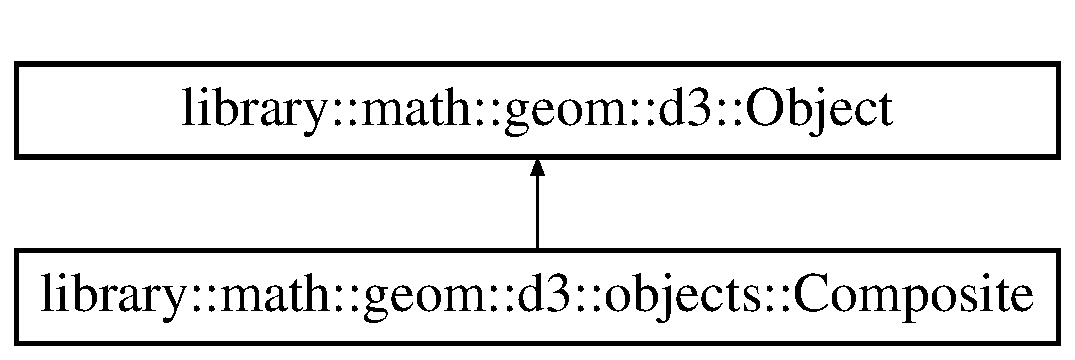
\includegraphics[height=2.000000cm]{classlibrary_1_1math_1_1geom_1_1d3_1_1objects_1_1_composite}
\end{center}
\end{figure}
\subsection*{Public Types}
\begin{DoxyCompactItemize}
\item 
typedef Array$<$ Unique$<$ \hyperlink{classlibrary_1_1math_1_1geom_1_1d3_1_1_object}{Object} $>$ $>$\+::\hyperlink{classlibrary_1_1math_1_1geom_1_1d3_1_1objects_1_1_composite_a52745f3c676ff98e099683b978253fc5}{Const\+Iterator} \hyperlink{classlibrary_1_1math_1_1geom_1_1d3_1_1objects_1_1_composite_a52745f3c676ff98e099683b978253fc5}{Const\+Iterator}
\end{DoxyCompactItemize}
\subsection*{Public Member Functions}
\begin{DoxyCompactItemize}
\item 
\hyperlink{classlibrary_1_1math_1_1geom_1_1d3_1_1objects_1_1_composite_a65acc162c125c6ad463b26f21cb87c39}{Composite} (const \hyperlink{classlibrary_1_1math_1_1geom_1_1d3_1_1_object}{Object} \&an\+Object)
\begin{DoxyCompactList}\small\item\em Constructor. \end{DoxyCompactList}\item 
\hyperlink{classlibrary_1_1math_1_1geom_1_1d3_1_1objects_1_1_composite_aae4a9ccbf373dbf2096b7ec34250f356}{Composite} (const Unique$<$ \hyperlink{classlibrary_1_1math_1_1geom_1_1d3_1_1_object}{Object} $>$ \&an\+Object\+U\+Ptr)
\begin{DoxyCompactList}\small\item\em Constructor. \end{DoxyCompactList}\item 
\hyperlink{classlibrary_1_1math_1_1geom_1_1d3_1_1objects_1_1_composite_aec95559cb5dc22f4f91ff63aa99bcc86}{Composite} (Array$<$ Unique$<$ \hyperlink{classlibrary_1_1math_1_1geom_1_1d3_1_1_object}{Object} $>$$>$ \&\&an\+Object\+Array)
\begin{DoxyCompactList}\small\item\em Constructor. \end{DoxyCompactList}\item 
\hyperlink{classlibrary_1_1math_1_1geom_1_1d3_1_1objects_1_1_composite_ab23551c7d923c428077edf5fa92cace9}{Composite} (const \hyperlink{classlibrary_1_1math_1_1geom_1_1d3_1_1objects_1_1_composite}{Composite} \&a\+Composite)
\begin{DoxyCompactList}\small\item\em Copy constructor. \end{DoxyCompactList}\item 
virtual \hyperlink{classlibrary_1_1math_1_1geom_1_1d3_1_1objects_1_1_composite}{Composite} $\ast$ \hyperlink{classlibrary_1_1math_1_1geom_1_1d3_1_1objects_1_1_composite_a8d1d598683fe3149498b55a089217686}{clone} () const override
\begin{DoxyCompactList}\small\item\em Clone composite. \end{DoxyCompactList}\item 
\hyperlink{classlibrary_1_1math_1_1geom_1_1d3_1_1objects_1_1_composite}{Composite} \& \hyperlink{classlibrary_1_1math_1_1geom_1_1d3_1_1objects_1_1_composite_ab33fc9368c5ee10fc1cd5d6baf08ef10}{operator=} (const \hyperlink{classlibrary_1_1math_1_1geom_1_1d3_1_1objects_1_1_composite}{Composite} \&a\+Composite)
\begin{DoxyCompactList}\small\item\em Copy assignment operator. \end{DoxyCompactList}\item 
bool \hyperlink{classlibrary_1_1math_1_1geom_1_1d3_1_1objects_1_1_composite_aaa79c2df606ffe1eac58aaa2cb5b39d2}{operator==} (const \hyperlink{classlibrary_1_1math_1_1geom_1_1d3_1_1objects_1_1_composite}{Composite} \&a\+Composite) const
\begin{DoxyCompactList}\small\item\em Equal to operator. \end{DoxyCompactList}\item 
bool \hyperlink{classlibrary_1_1math_1_1geom_1_1d3_1_1objects_1_1_composite_a8dbf350666d7dd33a4ada8f7172dab22}{operator!=} (const \hyperlink{classlibrary_1_1math_1_1geom_1_1d3_1_1objects_1_1_composite}{Composite} \&a\+Composite) const
\begin{DoxyCompactList}\small\item\em Not equal to operator. \end{DoxyCompactList}\item 
\hyperlink{classlibrary_1_1math_1_1geom_1_1d3_1_1objects_1_1_composite}{Composite} \hyperlink{classlibrary_1_1math_1_1geom_1_1d3_1_1objects_1_1_composite_a733b579f812eec28d898931c2597af8e}{operator+} (const \hyperlink{classlibrary_1_1math_1_1geom_1_1d3_1_1objects_1_1_composite}{Composite} \&a\+Composite) const
\begin{DoxyCompactList}\small\item\em Addition operator (composite concatenation) \end{DoxyCompactList}\item 
\hyperlink{classlibrary_1_1math_1_1geom_1_1d3_1_1objects_1_1_composite}{Composite} \& \hyperlink{classlibrary_1_1math_1_1geom_1_1d3_1_1objects_1_1_composite_aed5e20eedc5bd3094752bc71e73a85a6}{operator+=} (const \hyperlink{classlibrary_1_1math_1_1geom_1_1d3_1_1objects_1_1_composite}{Composite} \&a\+Composite)
\begin{DoxyCompactList}\small\item\em Addition assignment operator (composite concatenation) \end{DoxyCompactList}\item 
virtual bool \hyperlink{classlibrary_1_1math_1_1geom_1_1d3_1_1objects_1_1_composite_a6bc08a1686be837f6f8101a285d7351b}{is\+Defined} () const override
\begin{DoxyCompactList}\small\item\em Check if composite is defined. \end{DoxyCompactList}\item 
{\footnotesize template$<$class Type $>$ }\\bool \hyperlink{classlibrary_1_1math_1_1geom_1_1d3_1_1objects_1_1_composite_a93c70465b6f063fa98b7a99c22f380e7}{is} () const
\begin{DoxyCompactList}\small\item\em Returns true if composite can be converted to underlying object. \end{DoxyCompactList}\item 
{\footnotesize template$<$class Type $>$ }\\const Type \& \hyperlink{classlibrary_1_1math_1_1geom_1_1d3_1_1objects_1_1_composite_ac1cb85e31f4a4380f57f977ec35fca71}{as} () const
\begin{DoxyCompactList}\small\item\em Access composite as its underlying object. \end{DoxyCompactList}\item 
bool \hyperlink{classlibrary_1_1math_1_1geom_1_1d3_1_1objects_1_1_composite_abd37bc6f0b9132cee832d1628b76269c}{intersects} (const \hyperlink{classlibrary_1_1math_1_1geom_1_1d3_1_1_object}{Object} \&an\+Object) const
\begin{DoxyCompactList}\small\item\em Check if composite intersects object. \end{DoxyCompactList}\item 
bool \hyperlink{classlibrary_1_1math_1_1geom_1_1d3_1_1objects_1_1_composite_a38e1bd1a0bdc2623df25751307f2c834}{intersects} (const \hyperlink{classlibrary_1_1math_1_1geom_1_1d3_1_1objects_1_1_composite}{Composite} \&a\+Composite) const
\begin{DoxyCompactList}\small\item\em Check if composite intersects composite. \end{DoxyCompactList}\item 
bool \hyperlink{classlibrary_1_1math_1_1geom_1_1d3_1_1objects_1_1_composite_a3ec9ea04f09dea14be1e0f7eaa477c04}{contains} (const \hyperlink{classlibrary_1_1math_1_1geom_1_1d3_1_1_object}{Object} \&an\+Object) const
\begin{DoxyCompactList}\small\item\em Check if composite contains object. \end{DoxyCompactList}\item 
bool \hyperlink{classlibrary_1_1math_1_1geom_1_1d3_1_1objects_1_1_composite_a71c686259108546fd7a7415ff10bfea2}{contains} (const \hyperlink{classlibrary_1_1math_1_1geom_1_1d3_1_1objects_1_1_composite}{Composite} \&a\+Composite) const
\begin{DoxyCompactList}\small\item\em Check if composite contains composite. \end{DoxyCompactList}\item 
const \hyperlink{classlibrary_1_1math_1_1geom_1_1d3_1_1_object}{Object} \& \hyperlink{classlibrary_1_1math_1_1geom_1_1d3_1_1objects_1_1_composite_ab1f613a077a240c8193c58c77981a3b8}{access\+Object\+At} (const Index \&an\+Index) const
\begin{DoxyCompactList}\small\item\em Access object at index. \end{DoxyCompactList}\item 
const Array$<$ Unique$<$ \hyperlink{classlibrary_1_1math_1_1geom_1_1d3_1_1_object}{Object} $>$ $>$ \& \hyperlink{classlibrary_1_1math_1_1geom_1_1d3_1_1objects_1_1_composite_a1866df0e9b60a4badf60ad49ba7e9ea0}{access\+Objects} () const
\begin{DoxyCompactList}\small\item\em Access objects in composite. \end{DoxyCompactList}\item 
Size \hyperlink{classlibrary_1_1math_1_1geom_1_1d3_1_1objects_1_1_composite_ab97f7bd3d60450fc2f2b6a3b2a16cf5c}{get\+Object\+Count} () const
\begin{DoxyCompactList}\small\item\em Get number of objects in composite. \end{DoxyCompactList}\item 
\hyperlink{classlibrary_1_1math_1_1geom_1_1d3_1_1_intersection}{Intersection} \hyperlink{classlibrary_1_1math_1_1geom_1_1d3_1_1objects_1_1_composite_a5af4610cb68cb31bc5be14c06829c116}{intersection\+With} (const \hyperlink{classlibrary_1_1math_1_1geom_1_1d3_1_1_object}{Object} \&an\+Object) const
\begin{DoxyCompactList}\small\item\em Compute intersection of composite with object. \end{DoxyCompactList}\item 
\hyperlink{classlibrary_1_1math_1_1geom_1_1d3_1_1_intersection}{Intersection} \hyperlink{classlibrary_1_1math_1_1geom_1_1d3_1_1objects_1_1_composite_a56a243af1d865531cb56b99f607861ce}{intersection\+With} (const \hyperlink{classlibrary_1_1math_1_1geom_1_1d3_1_1objects_1_1_composite}{Composite} \&a\+Composite) const
\begin{DoxyCompactList}\small\item\em Compute intersection of composite with composite. \end{DoxyCompactList}\item 
\hyperlink{classlibrary_1_1math_1_1geom_1_1d3_1_1objects_1_1_composite_a52745f3c676ff98e099683b978253fc5}{Composite\+::\+Const\+Iterator} \hyperlink{classlibrary_1_1math_1_1geom_1_1d3_1_1objects_1_1_composite_ad2225ca4b70ef899e6bdd7ff7296c1d8}{begin} () const
\begin{DoxyCompactList}\small\item\em Get const iterator to begin. \end{DoxyCompactList}\item 
\hyperlink{classlibrary_1_1math_1_1geom_1_1d3_1_1objects_1_1_composite_a52745f3c676ff98e099683b978253fc5}{Composite\+::\+Const\+Iterator} \hyperlink{classlibrary_1_1math_1_1geom_1_1d3_1_1objects_1_1_composite_a17eb00b99b53fe9a483b05d7d4ef24aa}{end} () const
\begin{DoxyCompactList}\small\item\em Get const iterator to end. \end{DoxyCompactList}\item 
virtual void \hyperlink{classlibrary_1_1math_1_1geom_1_1d3_1_1objects_1_1_composite_adf6e594a816e509f7e85d51c84255236}{print} (std\+::ostream \&an\+Output\+Stream, bool display\+Decorators=true) const override
\begin{DoxyCompactList}\small\item\em Print composite. \end{DoxyCompactList}\item 
virtual void \hyperlink{classlibrary_1_1math_1_1geom_1_1d3_1_1objects_1_1_composite_a607850ccaeaea1dcd0cc57f986bea243}{apply\+Transformation} (const \hyperlink{classlibrary_1_1math_1_1geom_1_1d3_1_1_transformation}{Transformation} \&a\+Transformation) override
\begin{DoxyCompactList}\small\item\em Apply transformation to composite. \end{DoxyCompactList}\end{DoxyCompactItemize}
\subsection*{Static Public Member Functions}
\begin{DoxyCompactItemize}
\item 
static \hyperlink{classlibrary_1_1math_1_1geom_1_1d3_1_1objects_1_1_composite}{Composite} \hyperlink{classlibrary_1_1math_1_1geom_1_1d3_1_1objects_1_1_composite_a333ecb6ef3b6569330272d51eec83a01}{Undefined} ()
\begin{DoxyCompactList}\small\item\em Constructs an undefined composite. \end{DoxyCompactList}\end{DoxyCompactItemize}


\subsection{Detailed Description}
\hyperlink{classlibrary_1_1math_1_1geom_1_1d3_1_1objects_1_1_composite}{Composite} object. 

\subsection{Member Typedef Documentation}
\mbox{\Hypertarget{classlibrary_1_1math_1_1geom_1_1d3_1_1objects_1_1_composite_a52745f3c676ff98e099683b978253fc5}\label{classlibrary_1_1math_1_1geom_1_1d3_1_1objects_1_1_composite_a52745f3c676ff98e099683b978253fc5}} 
\index{library\+::math\+::geom\+::d3\+::objects\+::\+Composite@{library\+::math\+::geom\+::d3\+::objects\+::\+Composite}!Const\+Iterator@{Const\+Iterator}}
\index{Const\+Iterator@{Const\+Iterator}!library\+::math\+::geom\+::d3\+::objects\+::\+Composite@{library\+::math\+::geom\+::d3\+::objects\+::\+Composite}}
\subsubsection{\texorpdfstring{Const\+Iterator}{ConstIterator}}
{\footnotesize\ttfamily typedef Array$<$Unique$<$\hyperlink{classlibrary_1_1math_1_1geom_1_1d3_1_1_object}{Object}$>$ $>$\+::\hyperlink{classlibrary_1_1math_1_1geom_1_1d3_1_1objects_1_1_composite_a52745f3c676ff98e099683b978253fc5}{Const\+Iterator} \hyperlink{classlibrary_1_1math_1_1geom_1_1d3_1_1objects_1_1_composite_a52745f3c676ff98e099683b978253fc5}{library\+::math\+::geom\+::d3\+::objects\+::\+Composite\+::\+Const\+Iterator}}



\subsection{Constructor \& Destructor Documentation}
\mbox{\Hypertarget{classlibrary_1_1math_1_1geom_1_1d3_1_1objects_1_1_composite_a65acc162c125c6ad463b26f21cb87c39}\label{classlibrary_1_1math_1_1geom_1_1d3_1_1objects_1_1_composite_a65acc162c125c6ad463b26f21cb87c39}} 
\index{library\+::math\+::geom\+::d3\+::objects\+::\+Composite@{library\+::math\+::geom\+::d3\+::objects\+::\+Composite}!Composite@{Composite}}
\index{Composite@{Composite}!library\+::math\+::geom\+::d3\+::objects\+::\+Composite@{library\+::math\+::geom\+::d3\+::objects\+::\+Composite}}
\subsubsection{\texorpdfstring{Composite()}{Composite()}\hspace{0.1cm}{\footnotesize\ttfamily [1/4]}}
{\footnotesize\ttfamily library\+::math\+::geom\+::d3\+::objects\+::\+Composite\+::\+Composite (\begin{DoxyParamCaption}\item[{const \hyperlink{classlibrary_1_1math_1_1geom_1_1d3_1_1_object}{Object} \&}]{an\+Object }\end{DoxyParamCaption})\hspace{0.3cm}{\ttfamily [explicit]}}



Constructor. 


\begin{DoxyParams}[1]{Parameters}
\mbox{\tt in}  & {\em an\+Object} & An object \\
\hline
\end{DoxyParams}
\mbox{\Hypertarget{classlibrary_1_1math_1_1geom_1_1d3_1_1objects_1_1_composite_aae4a9ccbf373dbf2096b7ec34250f356}\label{classlibrary_1_1math_1_1geom_1_1d3_1_1objects_1_1_composite_aae4a9ccbf373dbf2096b7ec34250f356}} 
\index{library\+::math\+::geom\+::d3\+::objects\+::\+Composite@{library\+::math\+::geom\+::d3\+::objects\+::\+Composite}!Composite@{Composite}}
\index{Composite@{Composite}!library\+::math\+::geom\+::d3\+::objects\+::\+Composite@{library\+::math\+::geom\+::d3\+::objects\+::\+Composite}}
\subsubsection{\texorpdfstring{Composite()}{Composite()}\hspace{0.1cm}{\footnotesize\ttfamily [2/4]}}
{\footnotesize\ttfamily library\+::math\+::geom\+::d3\+::objects\+::\+Composite\+::\+Composite (\begin{DoxyParamCaption}\item[{const Unique$<$ \hyperlink{classlibrary_1_1math_1_1geom_1_1d3_1_1_object}{Object} $>$ \&}]{an\+Object\+U\+Ptr }\end{DoxyParamCaption})\hspace{0.3cm}{\ttfamily [explicit]}}



Constructor. 


\begin{DoxyParams}[1]{Parameters}
\mbox{\tt in}  & {\em an\+Object\+U\+Ptr} & A unique pointer to object \\
\hline
\end{DoxyParams}
\mbox{\Hypertarget{classlibrary_1_1math_1_1geom_1_1d3_1_1objects_1_1_composite_aec95559cb5dc22f4f91ff63aa99bcc86}\label{classlibrary_1_1math_1_1geom_1_1d3_1_1objects_1_1_composite_aec95559cb5dc22f4f91ff63aa99bcc86}} 
\index{library\+::math\+::geom\+::d3\+::objects\+::\+Composite@{library\+::math\+::geom\+::d3\+::objects\+::\+Composite}!Composite@{Composite}}
\index{Composite@{Composite}!library\+::math\+::geom\+::d3\+::objects\+::\+Composite@{library\+::math\+::geom\+::d3\+::objects\+::\+Composite}}
\subsubsection{\texorpdfstring{Composite()}{Composite()}\hspace{0.1cm}{\footnotesize\ttfamily [3/4]}}
{\footnotesize\ttfamily library\+::math\+::geom\+::d3\+::objects\+::\+Composite\+::\+Composite (\begin{DoxyParamCaption}\item[{Array$<$ Unique$<$ \hyperlink{classlibrary_1_1math_1_1geom_1_1d3_1_1_object}{Object} $>$$>$ \&\&}]{an\+Object\+Array }\end{DoxyParamCaption})\hspace{0.3cm}{\ttfamily [explicit]}}



Constructor. 


\begin{DoxyParams}[1]{Parameters}
\mbox{\tt in}  & {\em an\+Object\+Array} & An array of unique pointers to object \\
\hline
\end{DoxyParams}
\mbox{\Hypertarget{classlibrary_1_1math_1_1geom_1_1d3_1_1objects_1_1_composite_ab23551c7d923c428077edf5fa92cace9}\label{classlibrary_1_1math_1_1geom_1_1d3_1_1objects_1_1_composite_ab23551c7d923c428077edf5fa92cace9}} 
\index{library\+::math\+::geom\+::d3\+::objects\+::\+Composite@{library\+::math\+::geom\+::d3\+::objects\+::\+Composite}!Composite@{Composite}}
\index{Composite@{Composite}!library\+::math\+::geom\+::d3\+::objects\+::\+Composite@{library\+::math\+::geom\+::d3\+::objects\+::\+Composite}}
\subsubsection{\texorpdfstring{Composite()}{Composite()}\hspace{0.1cm}{\footnotesize\ttfamily [4/4]}}
{\footnotesize\ttfamily library\+::math\+::geom\+::d3\+::objects\+::\+Composite\+::\+Composite (\begin{DoxyParamCaption}\item[{const \hyperlink{classlibrary_1_1math_1_1geom_1_1d3_1_1objects_1_1_composite}{Composite} \&}]{a\+Composite }\end{DoxyParamCaption})}



Copy constructor. 


\begin{DoxyParams}[1]{Parameters}
\mbox{\tt in}  & {\em a\+Composite} & A composite \\
\hline
\end{DoxyParams}


\subsection{Member Function Documentation}
\mbox{\Hypertarget{classlibrary_1_1math_1_1geom_1_1d3_1_1objects_1_1_composite_ab1f613a077a240c8193c58c77981a3b8}\label{classlibrary_1_1math_1_1geom_1_1d3_1_1objects_1_1_composite_ab1f613a077a240c8193c58c77981a3b8}} 
\index{library\+::math\+::geom\+::d3\+::objects\+::\+Composite@{library\+::math\+::geom\+::d3\+::objects\+::\+Composite}!access\+Object\+At@{access\+Object\+At}}
\index{access\+Object\+At@{access\+Object\+At}!library\+::math\+::geom\+::d3\+::objects\+::\+Composite@{library\+::math\+::geom\+::d3\+::objects\+::\+Composite}}
\subsubsection{\texorpdfstring{access\+Object\+At()}{accessObjectAt()}}
{\footnotesize\ttfamily const \hyperlink{classlibrary_1_1math_1_1geom_1_1d3_1_1_object}{Object} \& library\+::math\+::geom\+::d3\+::objects\+::\+Composite\+::access\+Object\+At (\begin{DoxyParamCaption}\item[{const Index \&}]{an\+Index }\end{DoxyParamCaption}) const}



Access object at index. 


\begin{DoxyParams}[1]{Parameters}
\mbox{\tt in}  & {\em an\+Index} & An object index \\
\hline
\end{DoxyParams}
\begin{DoxyReturn}{Returns}
Reference to object 
\end{DoxyReturn}
\mbox{\Hypertarget{classlibrary_1_1math_1_1geom_1_1d3_1_1objects_1_1_composite_a1866df0e9b60a4badf60ad49ba7e9ea0}\label{classlibrary_1_1math_1_1geom_1_1d3_1_1objects_1_1_composite_a1866df0e9b60a4badf60ad49ba7e9ea0}} 
\index{library\+::math\+::geom\+::d3\+::objects\+::\+Composite@{library\+::math\+::geom\+::d3\+::objects\+::\+Composite}!access\+Objects@{access\+Objects}}
\index{access\+Objects@{access\+Objects}!library\+::math\+::geom\+::d3\+::objects\+::\+Composite@{library\+::math\+::geom\+::d3\+::objects\+::\+Composite}}
\subsubsection{\texorpdfstring{access\+Objects()}{accessObjects()}}
{\footnotesize\ttfamily const Array$<$ Unique$<$ \hyperlink{classlibrary_1_1math_1_1geom_1_1d3_1_1_object}{Object} $>$ $>$ \& library\+::math\+::geom\+::d3\+::objects\+::\+Composite\+::access\+Objects (\begin{DoxyParamCaption}{ }\end{DoxyParamCaption}) const}



Access objects in composite. 

\begin{DoxyReturn}{Returns}
Reference to objects in composite 
\end{DoxyReturn}
\mbox{\Hypertarget{classlibrary_1_1math_1_1geom_1_1d3_1_1objects_1_1_composite_a607850ccaeaea1dcd0cc57f986bea243}\label{classlibrary_1_1math_1_1geom_1_1d3_1_1objects_1_1_composite_a607850ccaeaea1dcd0cc57f986bea243}} 
\index{library\+::math\+::geom\+::d3\+::objects\+::\+Composite@{library\+::math\+::geom\+::d3\+::objects\+::\+Composite}!apply\+Transformation@{apply\+Transformation}}
\index{apply\+Transformation@{apply\+Transformation}!library\+::math\+::geom\+::d3\+::objects\+::\+Composite@{library\+::math\+::geom\+::d3\+::objects\+::\+Composite}}
\subsubsection{\texorpdfstring{apply\+Transformation()}{applyTransformation()}}
{\footnotesize\ttfamily void library\+::math\+::geom\+::d3\+::objects\+::\+Composite\+::apply\+Transformation (\begin{DoxyParamCaption}\item[{const \hyperlink{classlibrary_1_1math_1_1geom_1_1d3_1_1_transformation}{Transformation} \&}]{a\+Transformation }\end{DoxyParamCaption})\hspace{0.3cm}{\ttfamily [override]}, {\ttfamily [virtual]}}



Apply transformation to composite. 


\begin{DoxyParams}[1]{Parameters}
\mbox{\tt in}  & {\em a\+Transformation} & A transformation \\
\hline
\end{DoxyParams}


Implements \hyperlink{classlibrary_1_1math_1_1geom_1_1d3_1_1_object_a5fc47b1ee5d9a28efc6010d3d1512470}{library\+::math\+::geom\+::d3\+::\+Object}.

\mbox{\Hypertarget{classlibrary_1_1math_1_1geom_1_1d3_1_1objects_1_1_composite_ac1cb85e31f4a4380f57f977ec35fca71}\label{classlibrary_1_1math_1_1geom_1_1d3_1_1objects_1_1_composite_ac1cb85e31f4a4380f57f977ec35fca71}} 
\index{library\+::math\+::geom\+::d3\+::objects\+::\+Composite@{library\+::math\+::geom\+::d3\+::objects\+::\+Composite}!as@{as}}
\index{as@{as}!library\+::math\+::geom\+::d3\+::objects\+::\+Composite@{library\+::math\+::geom\+::d3\+::objects\+::\+Composite}}
\subsubsection{\texorpdfstring{as()}{as()}}
{\footnotesize\ttfamily template$<$class Type $>$ \\
const Type\& library\+::math\+::geom\+::d3\+::objects\+::\+Composite\+::as (\begin{DoxyParamCaption}{ }\end{DoxyParamCaption}) const\hspace{0.3cm}{\ttfamily [inline]}}



Access composite as its underlying object. 

Only valid if the composite only contains one object.

\begin{DoxyReturn}{Returns}
Reference to underlying object 
\end{DoxyReturn}
\mbox{\Hypertarget{classlibrary_1_1math_1_1geom_1_1d3_1_1objects_1_1_composite_ad2225ca4b70ef899e6bdd7ff7296c1d8}\label{classlibrary_1_1math_1_1geom_1_1d3_1_1objects_1_1_composite_ad2225ca4b70ef899e6bdd7ff7296c1d8}} 
\index{library\+::math\+::geom\+::d3\+::objects\+::\+Composite@{library\+::math\+::geom\+::d3\+::objects\+::\+Composite}!begin@{begin}}
\index{begin@{begin}!library\+::math\+::geom\+::d3\+::objects\+::\+Composite@{library\+::math\+::geom\+::d3\+::objects\+::\+Composite}}
\subsubsection{\texorpdfstring{begin()}{begin()}}
{\footnotesize\ttfamily \hyperlink{classlibrary_1_1math_1_1geom_1_1d3_1_1objects_1_1_composite_a52745f3c676ff98e099683b978253fc5}{Composite\+::\+Const\+Iterator} library\+::math\+::geom\+::d3\+::objects\+::\+Composite\+::begin (\begin{DoxyParamCaption}{ }\end{DoxyParamCaption}) const}



Get const iterator to begin. 

\begin{DoxyReturn}{Returns}
Const iterator to begin 
\end{DoxyReturn}
\mbox{\Hypertarget{classlibrary_1_1math_1_1geom_1_1d3_1_1objects_1_1_composite_a8d1d598683fe3149498b55a089217686}\label{classlibrary_1_1math_1_1geom_1_1d3_1_1objects_1_1_composite_a8d1d598683fe3149498b55a089217686}} 
\index{library\+::math\+::geom\+::d3\+::objects\+::\+Composite@{library\+::math\+::geom\+::d3\+::objects\+::\+Composite}!clone@{clone}}
\index{clone@{clone}!library\+::math\+::geom\+::d3\+::objects\+::\+Composite@{library\+::math\+::geom\+::d3\+::objects\+::\+Composite}}
\subsubsection{\texorpdfstring{clone()}{clone()}}
{\footnotesize\ttfamily \hyperlink{classlibrary_1_1math_1_1geom_1_1d3_1_1objects_1_1_composite}{Composite} $\ast$ library\+::math\+::geom\+::d3\+::objects\+::\+Composite\+::clone (\begin{DoxyParamCaption}{ }\end{DoxyParamCaption}) const\hspace{0.3cm}{\ttfamily [override]}, {\ttfamily [virtual]}}



Clone composite. 

\begin{DoxyReturn}{Returns}
Pointer to cloned composite 
\end{DoxyReturn}


Implements \hyperlink{classlibrary_1_1math_1_1geom_1_1d3_1_1_object_a1a784c6b359e0eb97cd34fabc42f2f3f}{library\+::math\+::geom\+::d3\+::\+Object}.

\mbox{\Hypertarget{classlibrary_1_1math_1_1geom_1_1d3_1_1objects_1_1_composite_a3ec9ea04f09dea14be1e0f7eaa477c04}\label{classlibrary_1_1math_1_1geom_1_1d3_1_1objects_1_1_composite_a3ec9ea04f09dea14be1e0f7eaa477c04}} 
\index{library\+::math\+::geom\+::d3\+::objects\+::\+Composite@{library\+::math\+::geom\+::d3\+::objects\+::\+Composite}!contains@{contains}}
\index{contains@{contains}!library\+::math\+::geom\+::d3\+::objects\+::\+Composite@{library\+::math\+::geom\+::d3\+::objects\+::\+Composite}}
\subsubsection{\texorpdfstring{contains()}{contains()}\hspace{0.1cm}{\footnotesize\ttfamily [1/2]}}
{\footnotesize\ttfamily bool library\+::math\+::geom\+::d3\+::objects\+::\+Composite\+::contains (\begin{DoxyParamCaption}\item[{const \hyperlink{classlibrary_1_1math_1_1geom_1_1d3_1_1_object}{Object} \&}]{an\+Object }\end{DoxyParamCaption}) const\hspace{0.3cm}{\ttfamily [virtual]}}



Check if composite contains object. 


\begin{DoxyParams}[1]{Parameters}
\mbox{\tt in}  & {\em an\+Object} & An object \\
\hline
\end{DoxyParams}
\begin{DoxyReturn}{Returns}
True if composite contains object 
\end{DoxyReturn}


Reimplemented from \hyperlink{classlibrary_1_1math_1_1geom_1_1d3_1_1_object_abaf45bf02ca165ba7bf685b24f5f97ef}{library\+::math\+::geom\+::d3\+::\+Object}.

\mbox{\Hypertarget{classlibrary_1_1math_1_1geom_1_1d3_1_1objects_1_1_composite_a71c686259108546fd7a7415ff10bfea2}\label{classlibrary_1_1math_1_1geom_1_1d3_1_1objects_1_1_composite_a71c686259108546fd7a7415ff10bfea2}} 
\index{library\+::math\+::geom\+::d3\+::objects\+::\+Composite@{library\+::math\+::geom\+::d3\+::objects\+::\+Composite}!contains@{contains}}
\index{contains@{contains}!library\+::math\+::geom\+::d3\+::objects\+::\+Composite@{library\+::math\+::geom\+::d3\+::objects\+::\+Composite}}
\subsubsection{\texorpdfstring{contains()}{contains()}\hspace{0.1cm}{\footnotesize\ttfamily [2/2]}}
{\footnotesize\ttfamily bool library\+::math\+::geom\+::d3\+::objects\+::\+Composite\+::contains (\begin{DoxyParamCaption}\item[{const \hyperlink{classlibrary_1_1math_1_1geom_1_1d3_1_1objects_1_1_composite}{Composite} \&}]{a\+Composite }\end{DoxyParamCaption}) const}



Check if composite contains composite. 


\begin{DoxyParams}[1]{Parameters}
\mbox{\tt in}  & {\em a\+Composite} & A composite \\
\hline
\end{DoxyParams}
\begin{DoxyReturn}{Returns}
True if composite contains composite 
\end{DoxyReturn}
\mbox{\Hypertarget{classlibrary_1_1math_1_1geom_1_1d3_1_1objects_1_1_composite_a17eb00b99b53fe9a483b05d7d4ef24aa}\label{classlibrary_1_1math_1_1geom_1_1d3_1_1objects_1_1_composite_a17eb00b99b53fe9a483b05d7d4ef24aa}} 
\index{library\+::math\+::geom\+::d3\+::objects\+::\+Composite@{library\+::math\+::geom\+::d3\+::objects\+::\+Composite}!end@{end}}
\index{end@{end}!library\+::math\+::geom\+::d3\+::objects\+::\+Composite@{library\+::math\+::geom\+::d3\+::objects\+::\+Composite}}
\subsubsection{\texorpdfstring{end()}{end()}}
{\footnotesize\ttfamily \hyperlink{classlibrary_1_1math_1_1geom_1_1d3_1_1objects_1_1_composite_a52745f3c676ff98e099683b978253fc5}{Composite\+::\+Const\+Iterator} library\+::math\+::geom\+::d3\+::objects\+::\+Composite\+::end (\begin{DoxyParamCaption}{ }\end{DoxyParamCaption}) const}



Get const iterator to end. 

\begin{DoxyReturn}{Returns}
Const iterator to end 
\end{DoxyReturn}
\mbox{\Hypertarget{classlibrary_1_1math_1_1geom_1_1d3_1_1objects_1_1_composite_ab97f7bd3d60450fc2f2b6a3b2a16cf5c}\label{classlibrary_1_1math_1_1geom_1_1d3_1_1objects_1_1_composite_ab97f7bd3d60450fc2f2b6a3b2a16cf5c}} 
\index{library\+::math\+::geom\+::d3\+::objects\+::\+Composite@{library\+::math\+::geom\+::d3\+::objects\+::\+Composite}!get\+Object\+Count@{get\+Object\+Count}}
\index{get\+Object\+Count@{get\+Object\+Count}!library\+::math\+::geom\+::d3\+::objects\+::\+Composite@{library\+::math\+::geom\+::d3\+::objects\+::\+Composite}}
\subsubsection{\texorpdfstring{get\+Object\+Count()}{getObjectCount()}}
{\footnotesize\ttfamily Size library\+::math\+::geom\+::d3\+::objects\+::\+Composite\+::get\+Object\+Count (\begin{DoxyParamCaption}{ }\end{DoxyParamCaption}) const}



Get number of objects in composite. 

\begin{DoxyReturn}{Returns}
Number of objects in composite 
\end{DoxyReturn}
\mbox{\Hypertarget{classlibrary_1_1math_1_1geom_1_1d3_1_1objects_1_1_composite_a5af4610cb68cb31bc5be14c06829c116}\label{classlibrary_1_1math_1_1geom_1_1d3_1_1objects_1_1_composite_a5af4610cb68cb31bc5be14c06829c116}} 
\index{library\+::math\+::geom\+::d3\+::objects\+::\+Composite@{library\+::math\+::geom\+::d3\+::objects\+::\+Composite}!intersection\+With@{intersection\+With}}
\index{intersection\+With@{intersection\+With}!library\+::math\+::geom\+::d3\+::objects\+::\+Composite@{library\+::math\+::geom\+::d3\+::objects\+::\+Composite}}
\subsubsection{\texorpdfstring{intersection\+With()}{intersectionWith()}\hspace{0.1cm}{\footnotesize\ttfamily [1/2]}}
{\footnotesize\ttfamily \hyperlink{classlibrary_1_1math_1_1geom_1_1d3_1_1_intersection}{Intersection} library\+::math\+::geom\+::d3\+::objects\+::\+Composite\+::intersection\+With (\begin{DoxyParamCaption}\item[{const \hyperlink{classlibrary_1_1math_1_1geom_1_1d3_1_1_object}{Object} \&}]{an\+Object }\end{DoxyParamCaption}) const\hspace{0.3cm}{\ttfamily [virtual]}}



Compute intersection of composite with object. 


\begin{DoxyParams}[1]{Parameters}
\mbox{\tt in}  & {\em an\+Object} & An object \\
\hline
\end{DoxyParams}
\begin{DoxyReturn}{Returns}
\hyperlink{classlibrary_1_1math_1_1geom_1_1d3_1_1_intersection}{Intersection} of composite with object 
\end{DoxyReturn}


Reimplemented from \hyperlink{classlibrary_1_1math_1_1geom_1_1d3_1_1_object_a609b1ea1d5f868b004726622efabad5d}{library\+::math\+::geom\+::d3\+::\+Object}.

\mbox{\Hypertarget{classlibrary_1_1math_1_1geom_1_1d3_1_1objects_1_1_composite_a56a243af1d865531cb56b99f607861ce}\label{classlibrary_1_1math_1_1geom_1_1d3_1_1objects_1_1_composite_a56a243af1d865531cb56b99f607861ce}} 
\index{library\+::math\+::geom\+::d3\+::objects\+::\+Composite@{library\+::math\+::geom\+::d3\+::objects\+::\+Composite}!intersection\+With@{intersection\+With}}
\index{intersection\+With@{intersection\+With}!library\+::math\+::geom\+::d3\+::objects\+::\+Composite@{library\+::math\+::geom\+::d3\+::objects\+::\+Composite}}
\subsubsection{\texorpdfstring{intersection\+With()}{intersectionWith()}\hspace{0.1cm}{\footnotesize\ttfamily [2/2]}}
{\footnotesize\ttfamily \hyperlink{classlibrary_1_1math_1_1geom_1_1d3_1_1_intersection}{Intersection} library\+::math\+::geom\+::d3\+::objects\+::\+Composite\+::intersection\+With (\begin{DoxyParamCaption}\item[{const \hyperlink{classlibrary_1_1math_1_1geom_1_1d3_1_1objects_1_1_composite}{Composite} \&}]{a\+Composite }\end{DoxyParamCaption}) const}



Compute intersection of composite with composite. 


\begin{DoxyParams}[1]{Parameters}
\mbox{\tt in}  & {\em a\+Composite} & A composite \\
\hline
\end{DoxyParams}
\begin{DoxyReturn}{Returns}
\hyperlink{classlibrary_1_1math_1_1geom_1_1d3_1_1_intersection}{Intersection} of composite with composite 
\end{DoxyReturn}
\mbox{\Hypertarget{classlibrary_1_1math_1_1geom_1_1d3_1_1objects_1_1_composite_abd37bc6f0b9132cee832d1628b76269c}\label{classlibrary_1_1math_1_1geom_1_1d3_1_1objects_1_1_composite_abd37bc6f0b9132cee832d1628b76269c}} 
\index{library\+::math\+::geom\+::d3\+::objects\+::\+Composite@{library\+::math\+::geom\+::d3\+::objects\+::\+Composite}!intersects@{intersects}}
\index{intersects@{intersects}!library\+::math\+::geom\+::d3\+::objects\+::\+Composite@{library\+::math\+::geom\+::d3\+::objects\+::\+Composite}}
\subsubsection{\texorpdfstring{intersects()}{intersects()}\hspace{0.1cm}{\footnotesize\ttfamily [1/2]}}
{\footnotesize\ttfamily bool library\+::math\+::geom\+::d3\+::objects\+::\+Composite\+::intersects (\begin{DoxyParamCaption}\item[{const \hyperlink{classlibrary_1_1math_1_1geom_1_1d3_1_1_object}{Object} \&}]{an\+Object }\end{DoxyParamCaption}) const\hspace{0.3cm}{\ttfamily [virtual]}}



Check if composite intersects object. 


\begin{DoxyParams}[1]{Parameters}
\mbox{\tt in}  & {\em an\+Object} & An object \\
\hline
\end{DoxyParams}
\begin{DoxyReturn}{Returns}
True if composite intersects object 
\end{DoxyReturn}


Reimplemented from \hyperlink{classlibrary_1_1math_1_1geom_1_1d3_1_1_object_a98c37b46f2fdc5f22bc123a757dcf73e}{library\+::math\+::geom\+::d3\+::\+Object}.

\mbox{\Hypertarget{classlibrary_1_1math_1_1geom_1_1d3_1_1objects_1_1_composite_a38e1bd1a0bdc2623df25751307f2c834}\label{classlibrary_1_1math_1_1geom_1_1d3_1_1objects_1_1_composite_a38e1bd1a0bdc2623df25751307f2c834}} 
\index{library\+::math\+::geom\+::d3\+::objects\+::\+Composite@{library\+::math\+::geom\+::d3\+::objects\+::\+Composite}!intersects@{intersects}}
\index{intersects@{intersects}!library\+::math\+::geom\+::d3\+::objects\+::\+Composite@{library\+::math\+::geom\+::d3\+::objects\+::\+Composite}}
\subsubsection{\texorpdfstring{intersects()}{intersects()}\hspace{0.1cm}{\footnotesize\ttfamily [2/2]}}
{\footnotesize\ttfamily bool library\+::math\+::geom\+::d3\+::objects\+::\+Composite\+::intersects (\begin{DoxyParamCaption}\item[{const \hyperlink{classlibrary_1_1math_1_1geom_1_1d3_1_1objects_1_1_composite}{Composite} \&}]{a\+Composite }\end{DoxyParamCaption}) const}



Check if composite intersects composite. 


\begin{DoxyParams}[1]{Parameters}
\mbox{\tt in}  & {\em a\+Composite} & A composite \\
\hline
\end{DoxyParams}
\begin{DoxyReturn}{Returns}
True if composite intersects composite 
\end{DoxyReturn}
\mbox{\Hypertarget{classlibrary_1_1math_1_1geom_1_1d3_1_1objects_1_1_composite_a93c70465b6f063fa98b7a99c22f380e7}\label{classlibrary_1_1math_1_1geom_1_1d3_1_1objects_1_1_composite_a93c70465b6f063fa98b7a99c22f380e7}} 
\index{library\+::math\+::geom\+::d3\+::objects\+::\+Composite@{library\+::math\+::geom\+::d3\+::objects\+::\+Composite}!is@{is}}
\index{is@{is}!library\+::math\+::geom\+::d3\+::objects\+::\+Composite@{library\+::math\+::geom\+::d3\+::objects\+::\+Composite}}
\subsubsection{\texorpdfstring{is()}{is()}}
{\footnotesize\ttfamily template$<$class Type $>$ \\
bool library\+::math\+::geom\+::d3\+::objects\+::\+Composite\+::is (\begin{DoxyParamCaption}{ }\end{DoxyParamCaption}) const\hspace{0.3cm}{\ttfamily [inline]}}



Returns true if composite can be converted to underlying object. 

Only valid if the composite only contains one object.

\begin{DoxyReturn}{Returns}
True if composite can be converted to underlying object 
\end{DoxyReturn}
\mbox{\Hypertarget{classlibrary_1_1math_1_1geom_1_1d3_1_1objects_1_1_composite_a6bc08a1686be837f6f8101a285d7351b}\label{classlibrary_1_1math_1_1geom_1_1d3_1_1objects_1_1_composite_a6bc08a1686be837f6f8101a285d7351b}} 
\index{library\+::math\+::geom\+::d3\+::objects\+::\+Composite@{library\+::math\+::geom\+::d3\+::objects\+::\+Composite}!is\+Defined@{is\+Defined}}
\index{is\+Defined@{is\+Defined}!library\+::math\+::geom\+::d3\+::objects\+::\+Composite@{library\+::math\+::geom\+::d3\+::objects\+::\+Composite}}
\subsubsection{\texorpdfstring{is\+Defined()}{isDefined()}}
{\footnotesize\ttfamily bool library\+::math\+::geom\+::d3\+::objects\+::\+Composite\+::is\+Defined (\begin{DoxyParamCaption}{ }\end{DoxyParamCaption}) const\hspace{0.3cm}{\ttfamily [override]}, {\ttfamily [virtual]}}



Check if composite is defined. 


\begin{DoxyCode}
\hyperlink{classlibrary_1_1math_1_1geom_1_1d3_1_1objects_1_1_composite_a65acc162c125c6ad463b26f21cb87c39}{Composite}(...).isDefined() ;
\end{DoxyCode}


\begin{DoxyReturn}{Returns}
True if composite is defined 
\end{DoxyReturn}


Implements \hyperlink{classlibrary_1_1math_1_1geom_1_1d3_1_1_object_a2216442e322f0c3ca5f01a4efa22baf7}{library\+::math\+::geom\+::d3\+::\+Object}.

\mbox{\Hypertarget{classlibrary_1_1math_1_1geom_1_1d3_1_1objects_1_1_composite_a8dbf350666d7dd33a4ada8f7172dab22}\label{classlibrary_1_1math_1_1geom_1_1d3_1_1objects_1_1_composite_a8dbf350666d7dd33a4ada8f7172dab22}} 
\index{library\+::math\+::geom\+::d3\+::objects\+::\+Composite@{library\+::math\+::geom\+::d3\+::objects\+::\+Composite}!operator"!=@{operator"!=}}
\index{operator"!=@{operator"!=}!library\+::math\+::geom\+::d3\+::objects\+::\+Composite@{library\+::math\+::geom\+::d3\+::objects\+::\+Composite}}
\subsubsection{\texorpdfstring{operator"!=()}{operator!=()}}
{\footnotesize\ttfamily bool library\+::math\+::geom\+::d3\+::objects\+::\+Composite\+::operator!= (\begin{DoxyParamCaption}\item[{const \hyperlink{classlibrary_1_1math_1_1geom_1_1d3_1_1objects_1_1_composite}{Composite} \&}]{a\+Composite }\end{DoxyParamCaption}) const}



Not equal to operator. 


\begin{DoxyParams}[1]{Parameters}
\mbox{\tt in}  & {\em a\+Composite} & A composite object \\
\hline
\end{DoxyParams}
\begin{DoxyReturn}{Returns}
True if composites are not equal 
\end{DoxyReturn}
\mbox{\Hypertarget{classlibrary_1_1math_1_1geom_1_1d3_1_1objects_1_1_composite_a733b579f812eec28d898931c2597af8e}\label{classlibrary_1_1math_1_1geom_1_1d3_1_1objects_1_1_composite_a733b579f812eec28d898931c2597af8e}} 
\index{library\+::math\+::geom\+::d3\+::objects\+::\+Composite@{library\+::math\+::geom\+::d3\+::objects\+::\+Composite}!operator+@{operator+}}
\index{operator+@{operator+}!library\+::math\+::geom\+::d3\+::objects\+::\+Composite@{library\+::math\+::geom\+::d3\+::objects\+::\+Composite}}
\subsubsection{\texorpdfstring{operator+()}{operator+()}}
{\footnotesize\ttfamily \hyperlink{classlibrary_1_1math_1_1geom_1_1d3_1_1objects_1_1_composite}{Composite} library\+::math\+::geom\+::d3\+::objects\+::\+Composite\+::operator+ (\begin{DoxyParamCaption}\item[{const \hyperlink{classlibrary_1_1math_1_1geom_1_1d3_1_1objects_1_1_composite}{Composite} \&}]{a\+Composite }\end{DoxyParamCaption}) const}



Addition operator (composite concatenation) 

Concatenate (merge) composite with another composite.


\begin{DoxyParams}[1]{Parameters}
\mbox{\tt in}  & {\em a\+Composite} & A composite \\
\hline
\end{DoxyParams}
\begin{DoxyReturn}{Returns}
Concatenated composite 
\end{DoxyReturn}
\mbox{\Hypertarget{classlibrary_1_1math_1_1geom_1_1d3_1_1objects_1_1_composite_aed5e20eedc5bd3094752bc71e73a85a6}\label{classlibrary_1_1math_1_1geom_1_1d3_1_1objects_1_1_composite_aed5e20eedc5bd3094752bc71e73a85a6}} 
\index{library\+::math\+::geom\+::d3\+::objects\+::\+Composite@{library\+::math\+::geom\+::d3\+::objects\+::\+Composite}!operator+=@{operator+=}}
\index{operator+=@{operator+=}!library\+::math\+::geom\+::d3\+::objects\+::\+Composite@{library\+::math\+::geom\+::d3\+::objects\+::\+Composite}}
\subsubsection{\texorpdfstring{operator+=()}{operator+=()}}
{\footnotesize\ttfamily \hyperlink{classlibrary_1_1math_1_1geom_1_1d3_1_1objects_1_1_composite}{Composite} \& library\+::math\+::geom\+::d3\+::objects\+::\+Composite\+::operator+= (\begin{DoxyParamCaption}\item[{const \hyperlink{classlibrary_1_1math_1_1geom_1_1d3_1_1objects_1_1_composite}{Composite} \&}]{a\+Composite }\end{DoxyParamCaption})}



Addition assignment operator (composite concatenation) 

Concatenate (merge) composite with another composite.


\begin{DoxyParams}[1]{Parameters}
\mbox{\tt in}  & {\em a\+Composite} & A composite \\
\hline
\end{DoxyParams}
\begin{DoxyReturn}{Returns}
Reference to concatenated composite 
\end{DoxyReturn}
\mbox{\Hypertarget{classlibrary_1_1math_1_1geom_1_1d3_1_1objects_1_1_composite_ab33fc9368c5ee10fc1cd5d6baf08ef10}\label{classlibrary_1_1math_1_1geom_1_1d3_1_1objects_1_1_composite_ab33fc9368c5ee10fc1cd5d6baf08ef10}} 
\index{library\+::math\+::geom\+::d3\+::objects\+::\+Composite@{library\+::math\+::geom\+::d3\+::objects\+::\+Composite}!operator=@{operator=}}
\index{operator=@{operator=}!library\+::math\+::geom\+::d3\+::objects\+::\+Composite@{library\+::math\+::geom\+::d3\+::objects\+::\+Composite}}
\subsubsection{\texorpdfstring{operator=()}{operator=()}}
{\footnotesize\ttfamily \hyperlink{classlibrary_1_1math_1_1geom_1_1d3_1_1objects_1_1_composite}{Composite} \& library\+::math\+::geom\+::d3\+::objects\+::\+Composite\+::operator= (\begin{DoxyParamCaption}\item[{const \hyperlink{classlibrary_1_1math_1_1geom_1_1d3_1_1objects_1_1_composite}{Composite} \&}]{a\+Composite }\end{DoxyParamCaption})}



Copy assignment operator. 


\begin{DoxyParams}[1]{Parameters}
\mbox{\tt in}  & {\em a\+Composite} & A composite \\
\hline
\end{DoxyParams}
\begin{DoxyReturn}{Returns}
Reference to composite 
\end{DoxyReturn}
\mbox{\Hypertarget{classlibrary_1_1math_1_1geom_1_1d3_1_1objects_1_1_composite_aaa79c2df606ffe1eac58aaa2cb5b39d2}\label{classlibrary_1_1math_1_1geom_1_1d3_1_1objects_1_1_composite_aaa79c2df606ffe1eac58aaa2cb5b39d2}} 
\index{library\+::math\+::geom\+::d3\+::objects\+::\+Composite@{library\+::math\+::geom\+::d3\+::objects\+::\+Composite}!operator==@{operator==}}
\index{operator==@{operator==}!library\+::math\+::geom\+::d3\+::objects\+::\+Composite@{library\+::math\+::geom\+::d3\+::objects\+::\+Composite}}
\subsubsection{\texorpdfstring{operator==()}{operator==()}}
{\footnotesize\ttfamily bool library\+::math\+::geom\+::d3\+::objects\+::\+Composite\+::operator== (\begin{DoxyParamCaption}\item[{const \hyperlink{classlibrary_1_1math_1_1geom_1_1d3_1_1objects_1_1_composite}{Composite} \&}]{a\+Composite }\end{DoxyParamCaption}) const}



Equal to operator. 


\begin{DoxyParams}[1]{Parameters}
\mbox{\tt in}  & {\em a\+Composite} & A composite object \\
\hline
\end{DoxyParams}
\begin{DoxyReturn}{Returns}
True if composites are equal 
\end{DoxyReturn}
\mbox{\Hypertarget{classlibrary_1_1math_1_1geom_1_1d3_1_1objects_1_1_composite_adf6e594a816e509f7e85d51c84255236}\label{classlibrary_1_1math_1_1geom_1_1d3_1_1objects_1_1_composite_adf6e594a816e509f7e85d51c84255236}} 
\index{library\+::math\+::geom\+::d3\+::objects\+::\+Composite@{library\+::math\+::geom\+::d3\+::objects\+::\+Composite}!print@{print}}
\index{print@{print}!library\+::math\+::geom\+::d3\+::objects\+::\+Composite@{library\+::math\+::geom\+::d3\+::objects\+::\+Composite}}
\subsubsection{\texorpdfstring{print()}{print()}}
{\footnotesize\ttfamily void library\+::math\+::geom\+::d3\+::objects\+::\+Composite\+::print (\begin{DoxyParamCaption}\item[{std\+::ostream \&}]{an\+Output\+Stream,  }\item[{bool}]{display\+Decorators = {\ttfamily true} }\end{DoxyParamCaption}) const\hspace{0.3cm}{\ttfamily [override]}, {\ttfamily [virtual]}}



Print composite. 


\begin{DoxyParams}[1]{Parameters}
\mbox{\tt in}  & {\em an\+Output\+Stream} & An output stream \\
\hline
\mbox{\tt in}  & {\em (optional)} & display\+Decorators If true, display decorators \\
\hline
\end{DoxyParams}


Implements \hyperlink{classlibrary_1_1math_1_1geom_1_1d3_1_1_object_aa166f4ce4d116a248f0fc861c75012ca}{library\+::math\+::geom\+::d3\+::\+Object}.

\mbox{\Hypertarget{classlibrary_1_1math_1_1geom_1_1d3_1_1objects_1_1_composite_a333ecb6ef3b6569330272d51eec83a01}\label{classlibrary_1_1math_1_1geom_1_1d3_1_1objects_1_1_composite_a333ecb6ef3b6569330272d51eec83a01}} 
\index{library\+::math\+::geom\+::d3\+::objects\+::\+Composite@{library\+::math\+::geom\+::d3\+::objects\+::\+Composite}!Undefined@{Undefined}}
\index{Undefined@{Undefined}!library\+::math\+::geom\+::d3\+::objects\+::\+Composite@{library\+::math\+::geom\+::d3\+::objects\+::\+Composite}}
\subsubsection{\texorpdfstring{Undefined()}{Undefined()}}
{\footnotesize\ttfamily \hyperlink{classlibrary_1_1math_1_1geom_1_1d3_1_1objects_1_1_composite}{Composite} library\+::math\+::geom\+::d3\+::objects\+::\+Composite\+::\+Undefined (\begin{DoxyParamCaption}{ }\end{DoxyParamCaption})\hspace{0.3cm}{\ttfamily [static]}}



Constructs an undefined composite. 


\begin{DoxyCode}
\hyperlink{classlibrary_1_1math_1_1geom_1_1d3_1_1objects_1_1_composite_a65acc162c125c6ad463b26f21cb87c39}{Composite} composite = \hyperlink{classlibrary_1_1math_1_1geom_1_1d3_1_1objects_1_1_composite_a333ecb6ef3b6569330272d51eec83a01}{Composite::Undefined}() ; \textcolor{comment}{// Undefined}
\end{DoxyCode}


\begin{DoxyReturn}{Returns}
Undefined composite 
\end{DoxyReturn}


The documentation for this class was generated from the following files\+:\begin{DoxyCompactItemize}
\item 
include/\+Library/\+Mathematics/\+Geometry/3\+D/\+Objects/\hyperlink{_composite_8hpp}{Composite.\+hpp}\item 
src/\+Library/\+Mathematics/\+Geometry/3\+D/\+Objects/\hyperlink{_composite_8cpp}{Composite.\+cpp}\end{DoxyCompactItemize}

\hypertarget{classlibrary_1_1math_1_1geom_1_1d3_1_1objects_1_1_cone}{}\section{library\+:\+:math\+:\+:geom\+:\+:d3\+:\+:objects\+:\+:Cone Class Reference}
\label{classlibrary_1_1math_1_1geom_1_1d3_1_1objects_1_1_cone}\index{library\+::math\+::geom\+::d3\+::objects\+::\+Cone@{library\+::math\+::geom\+::d3\+::objects\+::\+Cone}}


\hyperlink{classlibrary_1_1math_1_1geom_1_1d3_1_1objects_1_1_cone}{Cone}.  




{\ttfamily \#include $<$Cone.\+hpp$>$}

Inheritance diagram for library\+:\+:math\+:\+:geom\+:\+:d3\+:\+:objects\+:\+:Cone\+:\begin{figure}[H]
\begin{center}
\leavevmode
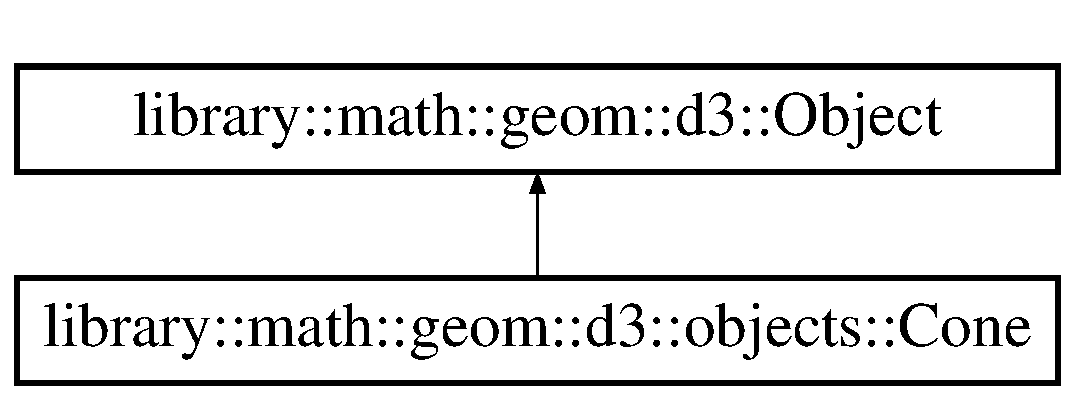
\includegraphics[height=2.000000cm]{classlibrary_1_1math_1_1geom_1_1d3_1_1objects_1_1_cone}
\end{center}
\end{figure}
\subsection*{Public Member Functions}
\begin{DoxyCompactItemize}
\item 
\hyperlink{classlibrary_1_1math_1_1geom_1_1d3_1_1objects_1_1_cone_a06829024b976d32cccc97fa2ee774670}{Cone} (const \hyperlink{classlibrary_1_1math_1_1geom_1_1d3_1_1objects_1_1_point}{Point} \&an\+Apex, const Vector3d \&an\+Axis, const \hyperlink{classlibrary_1_1math_1_1geom_1_1_angle}{Angle} \&an\+Angle)
\begin{DoxyCompactList}\small\item\em Constructor. \end{DoxyCompactList}\item 
virtual \hyperlink{classlibrary_1_1math_1_1geom_1_1d3_1_1objects_1_1_cone}{Cone} $\ast$ \hyperlink{classlibrary_1_1math_1_1geom_1_1d3_1_1objects_1_1_cone_a126e7d1918346a94032c6a925d24f045}{clone} () const override
\begin{DoxyCompactList}\small\item\em Clone cone. \end{DoxyCompactList}\item 
bool \hyperlink{classlibrary_1_1math_1_1geom_1_1d3_1_1objects_1_1_cone_a7535ef180acef7864bb3dfbb14952c7e}{operator==} (const \hyperlink{classlibrary_1_1math_1_1geom_1_1d3_1_1objects_1_1_cone}{Cone} \&a\+Cone) const
\begin{DoxyCompactList}\small\item\em Equal to operator. \end{DoxyCompactList}\item 
bool \hyperlink{classlibrary_1_1math_1_1geom_1_1d3_1_1objects_1_1_cone_a046cbc1e10c11a61e02eb5b9af904eef}{operator!=} (const \hyperlink{classlibrary_1_1math_1_1geom_1_1d3_1_1objects_1_1_cone}{Cone} \&a\+Cone) const
\begin{DoxyCompactList}\small\item\em Not equal to operator. \end{DoxyCompactList}\item 
virtual bool \hyperlink{classlibrary_1_1math_1_1geom_1_1d3_1_1objects_1_1_cone_aecfd56286894eb3f38789193a0768dc8}{is\+Defined} () const override
\begin{DoxyCompactList}\small\item\em Check if cone is defined. \end{DoxyCompactList}\item 
bool \hyperlink{classlibrary_1_1math_1_1geom_1_1d3_1_1objects_1_1_cone_a2ea8fa813ee4cd54a626e3468dbd845d}{intersects} (const \hyperlink{classlibrary_1_1math_1_1geom_1_1d3_1_1objects_1_1_sphere}{Sphere} \&a\+Sphere, const Size a\+Discretization\+Level=40) const
\begin{DoxyCompactList}\small\item\em Check if cone intersects sphere. \end{DoxyCompactList}\item 
bool \hyperlink{classlibrary_1_1math_1_1geom_1_1d3_1_1objects_1_1_cone_a05d41bcaf9428143d55b0f9ef83ace8b}{intersects} (const \hyperlink{classlibrary_1_1math_1_1geom_1_1d3_1_1objects_1_1_ellipsoid}{Ellipsoid} \&an\+Ellipsoid, const Size a\+Discretization\+Level=40) const
\begin{DoxyCompactList}\small\item\em Check if cone intersects ellipsoid. \end{DoxyCompactList}\item 
\hyperlink{classlibrary_1_1math_1_1geom_1_1d3_1_1objects_1_1_point}{Point} \hyperlink{classlibrary_1_1math_1_1geom_1_1d3_1_1objects_1_1_cone_a891fae1fe31a2a6c118059755887694c}{get\+Apex} () const
\begin{DoxyCompactList}\small\item\em Get cone apex. \end{DoxyCompactList}\item 
Vector3d \hyperlink{classlibrary_1_1math_1_1geom_1_1d3_1_1objects_1_1_cone_a9072972e480ef73f77b2ae4a6a0d8b78}{get\+Axis} () const
\begin{DoxyCompactList}\small\item\em Get cone axis. \end{DoxyCompactList}\item 
\hyperlink{classlibrary_1_1math_1_1geom_1_1_angle}{Angle} \hyperlink{classlibrary_1_1math_1_1geom_1_1d3_1_1objects_1_1_cone_a430aeb7c5f4855b01c929bbb9079596f}{get\+Angle} () const
\begin{DoxyCompactList}\small\item\em Get cone angle. \end{DoxyCompactList}\item 
Array$<$ \hyperlink{classlibrary_1_1math_1_1geom_1_1d3_1_1objects_1_1_ray}{Ray} $>$ \hyperlink{classlibrary_1_1math_1_1geom_1_1d3_1_1objects_1_1_cone_ad1f23b6a553f9856ecdafd633580ca2a}{get\+Rays\+Of\+Lateral\+Surface} (const Size a\+Ray\+Count=0) const
\begin{DoxyCompactList}\small\item\em Get rays of lateral surface. \end{DoxyCompactList}\item 
\hyperlink{classlibrary_1_1math_1_1geom_1_1d3_1_1_intersection}{Intersection} \hyperlink{classlibrary_1_1math_1_1geom_1_1d3_1_1objects_1_1_cone_ab49a0077e48c73a22726ecededf5553a}{intersection\+With} (const \hyperlink{classlibrary_1_1math_1_1geom_1_1d3_1_1objects_1_1_sphere}{Sphere} \&a\+Sphere, const bool only\+In\+Sight=false, const Size a\+Discretization\+Level=40) const
\begin{DoxyCompactList}\small\item\em Compute intersection of cone with sphere. \end{DoxyCompactList}\item 
\hyperlink{classlibrary_1_1math_1_1geom_1_1d3_1_1_intersection}{Intersection} \hyperlink{classlibrary_1_1math_1_1geom_1_1d3_1_1objects_1_1_cone_a2231a2ee1cd5464f04f2126eaee0973f}{intersection\+With} (const \hyperlink{classlibrary_1_1math_1_1geom_1_1d3_1_1objects_1_1_ellipsoid}{Ellipsoid} \&an\+Ellipsoid, const bool only\+In\+Sight=false, const Size a\+Discretization\+Level=40) const
\begin{DoxyCompactList}\small\item\em Compute intersection of cone with ellipsoid. \end{DoxyCompactList}\item 
virtual void \hyperlink{classlibrary_1_1math_1_1geom_1_1d3_1_1objects_1_1_cone_a1da79fa433164204f677bf247ce35538}{print} (std\+::ostream \&an\+Output\+Stream, bool display\+Decorators=true) const override
\begin{DoxyCompactList}\small\item\em Print cone. \end{DoxyCompactList}\item 
virtual void \hyperlink{classlibrary_1_1math_1_1geom_1_1d3_1_1objects_1_1_cone_a838ecaabc29abd32666342a7582a4a3e}{apply\+Transformation} (const \hyperlink{classlibrary_1_1math_1_1geom_1_1d3_1_1_transformation}{Transformation} \&a\+Transformation) override
\begin{DoxyCompactList}\small\item\em Apply transformation to cone. \end{DoxyCompactList}\end{DoxyCompactItemize}
\subsection*{Static Public Member Functions}
\begin{DoxyCompactItemize}
\item 
static \hyperlink{classlibrary_1_1math_1_1geom_1_1d3_1_1objects_1_1_cone}{Cone} \hyperlink{classlibrary_1_1math_1_1geom_1_1d3_1_1objects_1_1_cone_add91d1f26389385cca599be25cb18716}{Undefined} ()
\begin{DoxyCompactList}\small\item\em Constructs an undefined cone. \end{DoxyCompactList}\end{DoxyCompactItemize}


\subsection{Detailed Description}
\hyperlink{classlibrary_1_1math_1_1geom_1_1d3_1_1objects_1_1_cone}{Cone}. 

A cone is a three-\/dimensional geometric shape that tapers smoothly from a flat circular base to a point called the apex.

https\+://en.wikipedia.\+org/wiki/\+Cone 

\subsection{Constructor \& Destructor Documentation}
\mbox{\Hypertarget{classlibrary_1_1math_1_1geom_1_1d3_1_1objects_1_1_cone_a06829024b976d32cccc97fa2ee774670}\label{classlibrary_1_1math_1_1geom_1_1d3_1_1objects_1_1_cone_a06829024b976d32cccc97fa2ee774670}} 
\index{library\+::math\+::geom\+::d3\+::objects\+::\+Cone@{library\+::math\+::geom\+::d3\+::objects\+::\+Cone}!Cone@{Cone}}
\index{Cone@{Cone}!library\+::math\+::geom\+::d3\+::objects\+::\+Cone@{library\+::math\+::geom\+::d3\+::objects\+::\+Cone}}
\subsubsection{\texorpdfstring{Cone()}{Cone()}}
{\footnotesize\ttfamily library\+::math\+::geom\+::d3\+::objects\+::\+Cone\+::\+Cone (\begin{DoxyParamCaption}\item[{const \hyperlink{classlibrary_1_1math_1_1geom_1_1d3_1_1objects_1_1_point}{Point} \&}]{an\+Apex,  }\item[{const Vector3d \&}]{an\+Axis,  }\item[{const \hyperlink{classlibrary_1_1math_1_1geom_1_1_angle}{Angle} \&}]{an\+Angle }\end{DoxyParamCaption})}



Constructor. 


\begin{DoxyCode}
Point apex = \{ 0.0, 0.0, 0.0 \} ;
\hyperlink{namespacelibrary_1_1math_1_1obj_a977e84e9bf317a4e7dd9d6d671d6da2f}{Vector3d} axis = \{ 0.0, 0.0, 1.0 \} ;
Angle angle = \hyperlink{classlibrary_1_1math_1_1geom_1_1_angle_a64aa53e8420aeb6f671d86c65c370bc8}{Angle::Degrees}(15.0) ;
\hyperlink{classlibrary_1_1math_1_1geom_1_1d3_1_1objects_1_1_cone_a06829024b976d32cccc97fa2ee774670}{Cone} cone = \{ apex, axis, angle \} ;
\end{DoxyCode}



\begin{DoxyParams}[1]{Parameters}
\mbox{\tt in}  & {\em an\+Apex} & A cone apex \\
\hline
\mbox{\tt in}  & {\em an\+Axis} & A cone axis \\
\hline
\mbox{\tt in}  & {\em an\+Angle} & A cone angle \\
\hline
\end{DoxyParams}


\subsection{Member Function Documentation}
\mbox{\Hypertarget{classlibrary_1_1math_1_1geom_1_1d3_1_1objects_1_1_cone_a838ecaabc29abd32666342a7582a4a3e}\label{classlibrary_1_1math_1_1geom_1_1d3_1_1objects_1_1_cone_a838ecaabc29abd32666342a7582a4a3e}} 
\index{library\+::math\+::geom\+::d3\+::objects\+::\+Cone@{library\+::math\+::geom\+::d3\+::objects\+::\+Cone}!apply\+Transformation@{apply\+Transformation}}
\index{apply\+Transformation@{apply\+Transformation}!library\+::math\+::geom\+::d3\+::objects\+::\+Cone@{library\+::math\+::geom\+::d3\+::objects\+::\+Cone}}
\subsubsection{\texorpdfstring{apply\+Transformation()}{applyTransformation()}}
{\footnotesize\ttfamily void library\+::math\+::geom\+::d3\+::objects\+::\+Cone\+::apply\+Transformation (\begin{DoxyParamCaption}\item[{const \hyperlink{classlibrary_1_1math_1_1geom_1_1d3_1_1_transformation}{Transformation} \&}]{a\+Transformation }\end{DoxyParamCaption})\hspace{0.3cm}{\ttfamily [override]}, {\ttfamily [virtual]}}



Apply transformation to cone. 


\begin{DoxyParams}[1]{Parameters}
\mbox{\tt in}  & {\em a\+Transformation} & A transformation \\
\hline
\end{DoxyParams}


Implements \hyperlink{classlibrary_1_1math_1_1geom_1_1d3_1_1_object_a5fc47b1ee5d9a28efc6010d3d1512470}{library\+::math\+::geom\+::d3\+::\+Object}.

\mbox{\Hypertarget{classlibrary_1_1math_1_1geom_1_1d3_1_1objects_1_1_cone_a126e7d1918346a94032c6a925d24f045}\label{classlibrary_1_1math_1_1geom_1_1d3_1_1objects_1_1_cone_a126e7d1918346a94032c6a925d24f045}} 
\index{library\+::math\+::geom\+::d3\+::objects\+::\+Cone@{library\+::math\+::geom\+::d3\+::objects\+::\+Cone}!clone@{clone}}
\index{clone@{clone}!library\+::math\+::geom\+::d3\+::objects\+::\+Cone@{library\+::math\+::geom\+::d3\+::objects\+::\+Cone}}
\subsubsection{\texorpdfstring{clone()}{clone()}}
{\footnotesize\ttfamily \hyperlink{classlibrary_1_1math_1_1geom_1_1d3_1_1objects_1_1_cone}{Cone} $\ast$ library\+::math\+::geom\+::d3\+::objects\+::\+Cone\+::clone (\begin{DoxyParamCaption}{ }\end{DoxyParamCaption}) const\hspace{0.3cm}{\ttfamily [override]}, {\ttfamily [virtual]}}



Clone cone. 

\begin{DoxyReturn}{Returns}
Pointer to cloned cone 
\end{DoxyReturn}


Implements \hyperlink{classlibrary_1_1math_1_1geom_1_1d3_1_1_object_a1a784c6b359e0eb97cd34fabc42f2f3f}{library\+::math\+::geom\+::d3\+::\+Object}.

\mbox{\Hypertarget{classlibrary_1_1math_1_1geom_1_1d3_1_1objects_1_1_cone_a430aeb7c5f4855b01c929bbb9079596f}\label{classlibrary_1_1math_1_1geom_1_1d3_1_1objects_1_1_cone_a430aeb7c5f4855b01c929bbb9079596f}} 
\index{library\+::math\+::geom\+::d3\+::objects\+::\+Cone@{library\+::math\+::geom\+::d3\+::objects\+::\+Cone}!get\+Angle@{get\+Angle}}
\index{get\+Angle@{get\+Angle}!library\+::math\+::geom\+::d3\+::objects\+::\+Cone@{library\+::math\+::geom\+::d3\+::objects\+::\+Cone}}
\subsubsection{\texorpdfstring{get\+Angle()}{getAngle()}}
{\footnotesize\ttfamily \hyperlink{classlibrary_1_1math_1_1geom_1_1_angle}{Angle} library\+::math\+::geom\+::d3\+::objects\+::\+Cone\+::get\+Angle (\begin{DoxyParamCaption}{ }\end{DoxyParamCaption}) const}



Get cone angle. 

\begin{DoxyReturn}{Returns}
\hyperlink{classlibrary_1_1math_1_1geom_1_1d3_1_1objects_1_1_cone}{Cone} angle 
\end{DoxyReturn}
\mbox{\Hypertarget{classlibrary_1_1math_1_1geom_1_1d3_1_1objects_1_1_cone_a891fae1fe31a2a6c118059755887694c}\label{classlibrary_1_1math_1_1geom_1_1d3_1_1objects_1_1_cone_a891fae1fe31a2a6c118059755887694c}} 
\index{library\+::math\+::geom\+::d3\+::objects\+::\+Cone@{library\+::math\+::geom\+::d3\+::objects\+::\+Cone}!get\+Apex@{get\+Apex}}
\index{get\+Apex@{get\+Apex}!library\+::math\+::geom\+::d3\+::objects\+::\+Cone@{library\+::math\+::geom\+::d3\+::objects\+::\+Cone}}
\subsubsection{\texorpdfstring{get\+Apex()}{getApex()}}
{\footnotesize\ttfamily \hyperlink{classlibrary_1_1math_1_1geom_1_1d3_1_1objects_1_1_point}{Point} library\+::math\+::geom\+::d3\+::objects\+::\+Cone\+::get\+Apex (\begin{DoxyParamCaption}{ }\end{DoxyParamCaption}) const}



Get cone apex. 

\begin{DoxyReturn}{Returns}
\hyperlink{classlibrary_1_1math_1_1geom_1_1d3_1_1objects_1_1_cone}{Cone} apex 
\end{DoxyReturn}
\mbox{\Hypertarget{classlibrary_1_1math_1_1geom_1_1d3_1_1objects_1_1_cone_a9072972e480ef73f77b2ae4a6a0d8b78}\label{classlibrary_1_1math_1_1geom_1_1d3_1_1objects_1_1_cone_a9072972e480ef73f77b2ae4a6a0d8b78}} 
\index{library\+::math\+::geom\+::d3\+::objects\+::\+Cone@{library\+::math\+::geom\+::d3\+::objects\+::\+Cone}!get\+Axis@{get\+Axis}}
\index{get\+Axis@{get\+Axis}!library\+::math\+::geom\+::d3\+::objects\+::\+Cone@{library\+::math\+::geom\+::d3\+::objects\+::\+Cone}}
\subsubsection{\texorpdfstring{get\+Axis()}{getAxis()}}
{\footnotesize\ttfamily Vector3d library\+::math\+::geom\+::d3\+::objects\+::\+Cone\+::get\+Axis (\begin{DoxyParamCaption}{ }\end{DoxyParamCaption}) const}



Get cone axis. 

\begin{DoxyReturn}{Returns}
\hyperlink{classlibrary_1_1math_1_1geom_1_1d3_1_1objects_1_1_cone}{Cone} axis 
\end{DoxyReturn}
\mbox{\Hypertarget{classlibrary_1_1math_1_1geom_1_1d3_1_1objects_1_1_cone_ad1f23b6a553f9856ecdafd633580ca2a}\label{classlibrary_1_1math_1_1geom_1_1d3_1_1objects_1_1_cone_ad1f23b6a553f9856ecdafd633580ca2a}} 
\index{library\+::math\+::geom\+::d3\+::objects\+::\+Cone@{library\+::math\+::geom\+::d3\+::objects\+::\+Cone}!get\+Rays\+Of\+Lateral\+Surface@{get\+Rays\+Of\+Lateral\+Surface}}
\index{get\+Rays\+Of\+Lateral\+Surface@{get\+Rays\+Of\+Lateral\+Surface}!library\+::math\+::geom\+::d3\+::objects\+::\+Cone@{library\+::math\+::geom\+::d3\+::objects\+::\+Cone}}
\subsubsection{\texorpdfstring{get\+Rays\+Of\+Lateral\+Surface()}{getRaysOfLateralSurface()}}
{\footnotesize\ttfamily Array$<$ \hyperlink{classlibrary_1_1math_1_1geom_1_1d3_1_1objects_1_1_ray}{Ray} $>$ library\+::math\+::geom\+::d3\+::objects\+::\+Cone\+::get\+Rays\+Of\+Lateral\+Surface (\begin{DoxyParamCaption}\item[{const Size}]{a\+Ray\+Count = {\ttfamily 0} }\end{DoxyParamCaption}) const}



Get rays of lateral surface. 


\begin{DoxyParams}[1]{Parameters}
\mbox{\tt in}  & {\em a\+Ray\+Count} & A number of rays (at least face count) \\
\hline
\end{DoxyParams}
\begin{DoxyReturn}{Returns}
Array of rays 
\end{DoxyReturn}
\mbox{\Hypertarget{classlibrary_1_1math_1_1geom_1_1d3_1_1objects_1_1_cone_ab49a0077e48c73a22726ecededf5553a}\label{classlibrary_1_1math_1_1geom_1_1d3_1_1objects_1_1_cone_ab49a0077e48c73a22726ecededf5553a}} 
\index{library\+::math\+::geom\+::d3\+::objects\+::\+Cone@{library\+::math\+::geom\+::d3\+::objects\+::\+Cone}!intersection\+With@{intersection\+With}}
\index{intersection\+With@{intersection\+With}!library\+::math\+::geom\+::d3\+::objects\+::\+Cone@{library\+::math\+::geom\+::d3\+::objects\+::\+Cone}}
\subsubsection{\texorpdfstring{intersection\+With()}{intersectionWith()}\hspace{0.1cm}{\footnotesize\ttfamily [1/2]}}
{\footnotesize\ttfamily \hyperlink{classlibrary_1_1math_1_1geom_1_1d3_1_1_intersection}{Intersection} library\+::math\+::geom\+::d3\+::objects\+::\+Cone\+::intersection\+With (\begin{DoxyParamCaption}\item[{const \hyperlink{classlibrary_1_1math_1_1geom_1_1d3_1_1objects_1_1_sphere}{Sphere} \&}]{a\+Sphere,  }\item[{const bool}]{only\+In\+Sight = {\ttfamily false},  }\item[{const Size}]{a\+Discretization\+Level = {\ttfamily 40} }\end{DoxyParamCaption}) const}



Compute intersection of cone with sphere. 


\begin{DoxyParams}[1]{Parameters}
\mbox{\tt in}  & {\em a\+Sphere} & A sphere \\
\hline
\mbox{\tt in}  & {\em only\+In\+Sight} & (optional) If true, only return intersection points that are in sight \\
\hline
\mbox{\tt in}  & {\em a\+Discretization\+Level} & (optional) The polygonal discretization level \\
\hline
\end{DoxyParams}
\begin{DoxyReturn}{Returns}
\hyperlink{classlibrary_1_1math_1_1geom_1_1d3_1_1_intersection}{Intersection} of cone with sphere 
\end{DoxyReturn}
\mbox{\Hypertarget{classlibrary_1_1math_1_1geom_1_1d3_1_1objects_1_1_cone_a2231a2ee1cd5464f04f2126eaee0973f}\label{classlibrary_1_1math_1_1geom_1_1d3_1_1objects_1_1_cone_a2231a2ee1cd5464f04f2126eaee0973f}} 
\index{library\+::math\+::geom\+::d3\+::objects\+::\+Cone@{library\+::math\+::geom\+::d3\+::objects\+::\+Cone}!intersection\+With@{intersection\+With}}
\index{intersection\+With@{intersection\+With}!library\+::math\+::geom\+::d3\+::objects\+::\+Cone@{library\+::math\+::geom\+::d3\+::objects\+::\+Cone}}
\subsubsection{\texorpdfstring{intersection\+With()}{intersectionWith()}\hspace{0.1cm}{\footnotesize\ttfamily [2/2]}}
{\footnotesize\ttfamily \hyperlink{classlibrary_1_1math_1_1geom_1_1d3_1_1_intersection}{Intersection} library\+::math\+::geom\+::d3\+::objects\+::\+Cone\+::intersection\+With (\begin{DoxyParamCaption}\item[{const \hyperlink{classlibrary_1_1math_1_1geom_1_1d3_1_1objects_1_1_ellipsoid}{Ellipsoid} \&}]{an\+Ellipsoid,  }\item[{const bool}]{only\+In\+Sight = {\ttfamily false},  }\item[{const Size}]{a\+Discretization\+Level = {\ttfamily 40} }\end{DoxyParamCaption}) const}



Compute intersection of cone with ellipsoid. 


\begin{DoxyParams}[1]{Parameters}
\mbox{\tt in}  & {\em an\+Ellipsoid} & An ellipsoid \\
\hline
\mbox{\tt in}  & {\em only\+In\+Sight} & (optional) If true, only return intersection points that are in sight \\
\hline
\mbox{\tt in}  & {\em a\+Discretization\+Level} & (optional) The polygonal discretization level \\
\hline
\end{DoxyParams}
\begin{DoxyReturn}{Returns}
\hyperlink{classlibrary_1_1math_1_1geom_1_1d3_1_1_intersection}{Intersection} of cone with ellipsoid 
\end{DoxyReturn}
\mbox{\Hypertarget{classlibrary_1_1math_1_1geom_1_1d3_1_1objects_1_1_cone_a2ea8fa813ee4cd54a626e3468dbd845d}\label{classlibrary_1_1math_1_1geom_1_1d3_1_1objects_1_1_cone_a2ea8fa813ee4cd54a626e3468dbd845d}} 
\index{library\+::math\+::geom\+::d3\+::objects\+::\+Cone@{library\+::math\+::geom\+::d3\+::objects\+::\+Cone}!intersects@{intersects}}
\index{intersects@{intersects}!library\+::math\+::geom\+::d3\+::objects\+::\+Cone@{library\+::math\+::geom\+::d3\+::objects\+::\+Cone}}
\subsubsection{\texorpdfstring{intersects()}{intersects()}\hspace{0.1cm}{\footnotesize\ttfamily [1/2]}}
{\footnotesize\ttfamily bool library\+::math\+::geom\+::d3\+::objects\+::\+Cone\+::intersects (\begin{DoxyParamCaption}\item[{const \hyperlink{classlibrary_1_1math_1_1geom_1_1d3_1_1objects_1_1_sphere}{Sphere} \&}]{a\+Sphere,  }\item[{const Size}]{a\+Discretization\+Level = {\ttfamily 40} }\end{DoxyParamCaption}) const}



Check if cone intersects sphere. 


\begin{DoxyCode}
\hyperlink{classlibrary_1_1math_1_1geom_1_1d3_1_1objects_1_1_cone_a06829024b976d32cccc97fa2ee774670}{Cone} cone = ... ;
Sphere sphere = ... ;
cone.intersects(sphere) ;
\end{DoxyCode}



\begin{DoxyParams}[1]{Parameters}
\mbox{\tt in}  & {\em a\+Sphere} & A sphere \\
\hline
\mbox{\tt in}  & {\em a\+Discretization\+Level} & (optional) The polygonal discretization level \\
\hline
\end{DoxyParams}
\begin{DoxyReturn}{Returns}
True if cone intersects sphere 
\end{DoxyReturn}
\mbox{\Hypertarget{classlibrary_1_1math_1_1geom_1_1d3_1_1objects_1_1_cone_a05d41bcaf9428143d55b0f9ef83ace8b}\label{classlibrary_1_1math_1_1geom_1_1d3_1_1objects_1_1_cone_a05d41bcaf9428143d55b0f9ef83ace8b}} 
\index{library\+::math\+::geom\+::d3\+::objects\+::\+Cone@{library\+::math\+::geom\+::d3\+::objects\+::\+Cone}!intersects@{intersects}}
\index{intersects@{intersects}!library\+::math\+::geom\+::d3\+::objects\+::\+Cone@{library\+::math\+::geom\+::d3\+::objects\+::\+Cone}}
\subsubsection{\texorpdfstring{intersects()}{intersects()}\hspace{0.1cm}{\footnotesize\ttfamily [2/2]}}
{\footnotesize\ttfamily bool library\+::math\+::geom\+::d3\+::objects\+::\+Cone\+::intersects (\begin{DoxyParamCaption}\item[{const \hyperlink{classlibrary_1_1math_1_1geom_1_1d3_1_1objects_1_1_ellipsoid}{Ellipsoid} \&}]{an\+Ellipsoid,  }\item[{const Size}]{a\+Discretization\+Level = {\ttfamily 40} }\end{DoxyParamCaption}) const}



Check if cone intersects ellipsoid. 


\begin{DoxyCode}
\hyperlink{classlibrary_1_1math_1_1geom_1_1d3_1_1objects_1_1_cone_a06829024b976d32cccc97fa2ee774670}{Cone} cone = ... ;
Ellipsoid ellipsoid = ... ;
cone.intersects(ellipsoid) ;
\end{DoxyCode}



\begin{DoxyParams}[1]{Parameters}
\mbox{\tt in}  & {\em an\+Ellipsoid} & An ellipsoid \\
\hline
\mbox{\tt in}  & {\em a\+Discretization\+Level} & (optional) The polygonal discretization level \\
\hline
\end{DoxyParams}
\begin{DoxyReturn}{Returns}
True if cone intersects ellipsoid 
\end{DoxyReturn}
\mbox{\Hypertarget{classlibrary_1_1math_1_1geom_1_1d3_1_1objects_1_1_cone_aecfd56286894eb3f38789193a0768dc8}\label{classlibrary_1_1math_1_1geom_1_1d3_1_1objects_1_1_cone_aecfd56286894eb3f38789193a0768dc8}} 
\index{library\+::math\+::geom\+::d3\+::objects\+::\+Cone@{library\+::math\+::geom\+::d3\+::objects\+::\+Cone}!is\+Defined@{is\+Defined}}
\index{is\+Defined@{is\+Defined}!library\+::math\+::geom\+::d3\+::objects\+::\+Cone@{library\+::math\+::geom\+::d3\+::objects\+::\+Cone}}
\subsubsection{\texorpdfstring{is\+Defined()}{isDefined()}}
{\footnotesize\ttfamily bool library\+::math\+::geom\+::d3\+::objects\+::\+Cone\+::is\+Defined (\begin{DoxyParamCaption}{ }\end{DoxyParamCaption}) const\hspace{0.3cm}{\ttfamily [override]}, {\ttfamily [virtual]}}



Check if cone is defined. 

\begin{DoxyReturn}{Returns}
True if cone is defined 
\end{DoxyReturn}


Implements \hyperlink{classlibrary_1_1math_1_1geom_1_1d3_1_1_object_a2216442e322f0c3ca5f01a4efa22baf7}{library\+::math\+::geom\+::d3\+::\+Object}.

\mbox{\Hypertarget{classlibrary_1_1math_1_1geom_1_1d3_1_1objects_1_1_cone_a046cbc1e10c11a61e02eb5b9af904eef}\label{classlibrary_1_1math_1_1geom_1_1d3_1_1objects_1_1_cone_a046cbc1e10c11a61e02eb5b9af904eef}} 
\index{library\+::math\+::geom\+::d3\+::objects\+::\+Cone@{library\+::math\+::geom\+::d3\+::objects\+::\+Cone}!operator"!=@{operator"!=}}
\index{operator"!=@{operator"!=}!library\+::math\+::geom\+::d3\+::objects\+::\+Cone@{library\+::math\+::geom\+::d3\+::objects\+::\+Cone}}
\subsubsection{\texorpdfstring{operator"!=()}{operator!=()}}
{\footnotesize\ttfamily bool library\+::math\+::geom\+::d3\+::objects\+::\+Cone\+::operator!= (\begin{DoxyParamCaption}\item[{const \hyperlink{classlibrary_1_1math_1_1geom_1_1d3_1_1objects_1_1_cone}{Cone} \&}]{a\+Cone }\end{DoxyParamCaption}) const}



Not equal to operator. 


\begin{DoxyParams}[1]{Parameters}
\mbox{\tt in}  & {\em a\+Cone} & A cone \\
\hline
\end{DoxyParams}
\begin{DoxyReturn}{Returns}
True if cones are not equal 
\end{DoxyReturn}
\mbox{\Hypertarget{classlibrary_1_1math_1_1geom_1_1d3_1_1objects_1_1_cone_a7535ef180acef7864bb3dfbb14952c7e}\label{classlibrary_1_1math_1_1geom_1_1d3_1_1objects_1_1_cone_a7535ef180acef7864bb3dfbb14952c7e}} 
\index{library\+::math\+::geom\+::d3\+::objects\+::\+Cone@{library\+::math\+::geom\+::d3\+::objects\+::\+Cone}!operator==@{operator==}}
\index{operator==@{operator==}!library\+::math\+::geom\+::d3\+::objects\+::\+Cone@{library\+::math\+::geom\+::d3\+::objects\+::\+Cone}}
\subsubsection{\texorpdfstring{operator==()}{operator==()}}
{\footnotesize\ttfamily bool library\+::math\+::geom\+::d3\+::objects\+::\+Cone\+::operator== (\begin{DoxyParamCaption}\item[{const \hyperlink{classlibrary_1_1math_1_1geom_1_1d3_1_1objects_1_1_cone}{Cone} \&}]{a\+Cone }\end{DoxyParamCaption}) const}



Equal to operator. 


\begin{DoxyParams}[1]{Parameters}
\mbox{\tt in}  & {\em a\+Cone} & A cone \\
\hline
\end{DoxyParams}
\begin{DoxyReturn}{Returns}
True if cones are equal 
\end{DoxyReturn}
\mbox{\Hypertarget{classlibrary_1_1math_1_1geom_1_1d3_1_1objects_1_1_cone_a1da79fa433164204f677bf247ce35538}\label{classlibrary_1_1math_1_1geom_1_1d3_1_1objects_1_1_cone_a1da79fa433164204f677bf247ce35538}} 
\index{library\+::math\+::geom\+::d3\+::objects\+::\+Cone@{library\+::math\+::geom\+::d3\+::objects\+::\+Cone}!print@{print}}
\index{print@{print}!library\+::math\+::geom\+::d3\+::objects\+::\+Cone@{library\+::math\+::geom\+::d3\+::objects\+::\+Cone}}
\subsubsection{\texorpdfstring{print()}{print()}}
{\footnotesize\ttfamily void library\+::math\+::geom\+::d3\+::objects\+::\+Cone\+::print (\begin{DoxyParamCaption}\item[{std\+::ostream \&}]{an\+Output\+Stream,  }\item[{bool}]{display\+Decorators = {\ttfamily true} }\end{DoxyParamCaption}) const\hspace{0.3cm}{\ttfamily [override]}, {\ttfamily [virtual]}}



Print cone. 


\begin{DoxyParams}[1]{Parameters}
\mbox{\tt in}  & {\em an\+Output\+Stream} & An output stream \\
\hline
\mbox{\tt in}  & {\em (optional)} & display\+Decorators If true, display decorators \\
\hline
\end{DoxyParams}


Implements \hyperlink{classlibrary_1_1math_1_1geom_1_1d3_1_1_object_aa166f4ce4d116a248f0fc861c75012ca}{library\+::math\+::geom\+::d3\+::\+Object}.

\mbox{\Hypertarget{classlibrary_1_1math_1_1geom_1_1d3_1_1objects_1_1_cone_add91d1f26389385cca599be25cb18716}\label{classlibrary_1_1math_1_1geom_1_1d3_1_1objects_1_1_cone_add91d1f26389385cca599be25cb18716}} 
\index{library\+::math\+::geom\+::d3\+::objects\+::\+Cone@{library\+::math\+::geom\+::d3\+::objects\+::\+Cone}!Undefined@{Undefined}}
\index{Undefined@{Undefined}!library\+::math\+::geom\+::d3\+::objects\+::\+Cone@{library\+::math\+::geom\+::d3\+::objects\+::\+Cone}}
\subsubsection{\texorpdfstring{Undefined()}{Undefined()}}
{\footnotesize\ttfamily \hyperlink{classlibrary_1_1math_1_1geom_1_1d3_1_1objects_1_1_cone}{Cone} library\+::math\+::geom\+::d3\+::objects\+::\+Cone\+::\+Undefined (\begin{DoxyParamCaption}{ }\end{DoxyParamCaption})\hspace{0.3cm}{\ttfamily [static]}}



Constructs an undefined cone. 

\begin{DoxyReturn}{Returns}
Undefined cone 
\end{DoxyReturn}


The documentation for this class was generated from the following files\+:\begin{DoxyCompactItemize}
\item 
include/\+Library/\+Mathematics/\+Geometry/3\+D/\+Objects/\hyperlink{_cone_8hpp}{Cone.\+hpp}\item 
src/\+Library/\+Mathematics/\+Geometry/3\+D/\+Objects/\hyperlink{_cone_8cpp}{Cone.\+cpp}\end{DoxyCompactItemize}

\hypertarget{classlibrary_1_1math_1_1geom_1_1d3_1_1objects_1_1_cuboid}{}\section{library\+:\+:math\+:\+:geom\+:\+:d3\+:\+:objects\+:\+:Cuboid Class Reference}
\label{classlibrary_1_1math_1_1geom_1_1d3_1_1objects_1_1_cuboid}\index{library\+::math\+::geom\+::d3\+::objects\+::\+Cuboid@{library\+::math\+::geom\+::d3\+::objects\+::\+Cuboid}}


\hyperlink{classlibrary_1_1math_1_1geom_1_1d3_1_1objects_1_1_cuboid}{Cuboid}.  




{\ttfamily \#include $<$Cuboid.\+hpp$>$}

Inheritance diagram for library\+:\+:math\+:\+:geom\+:\+:d3\+:\+:objects\+:\+:Cuboid\+:\begin{figure}[H]
\begin{center}
\leavevmode
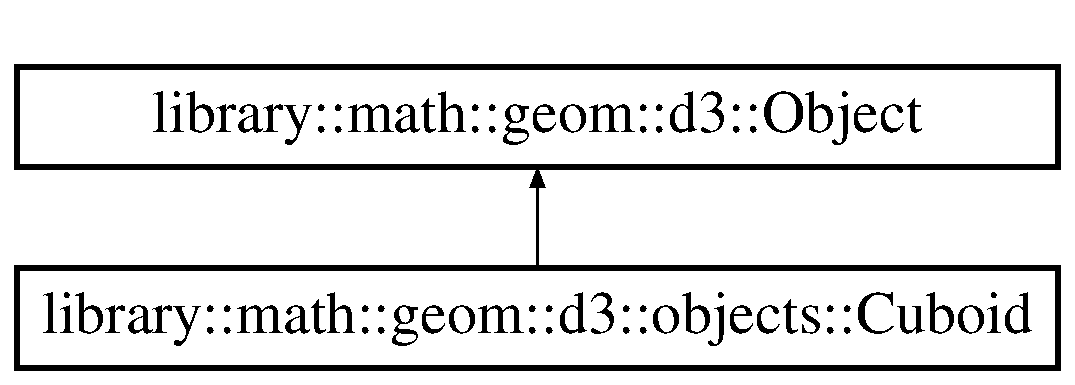
\includegraphics[height=2.000000cm]{classlibrary_1_1math_1_1geom_1_1d3_1_1objects_1_1_cuboid}
\end{center}
\end{figure}
\subsection*{Public Types}
\begin{DoxyCompactItemize}
\item 
typedef \hyperlink{classlibrary_1_1math_1_1geom_1_1d3_1_1objects_1_1_point}{Point} \hyperlink{classlibrary_1_1math_1_1geom_1_1d3_1_1objects_1_1_cuboid_ad9600791c8ac7f1253dc94417ec12f3c}{Vertex}
\item 
typedef \hyperlink{classlibrary_1_1math_1_1geom_1_1d3_1_1objects_1_1_segment}{Segment} \hyperlink{classlibrary_1_1math_1_1geom_1_1d3_1_1objects_1_1_cuboid_a743ee54e5fb8e2e649c254e69abed69c}{Edge}
\end{DoxyCompactItemize}
\subsection*{Public Member Functions}
\begin{DoxyCompactItemize}
\item 
\hyperlink{classlibrary_1_1math_1_1geom_1_1d3_1_1objects_1_1_cuboid_ac42299f962fab284a76a46d4ea4e6fa2}{Cuboid} (const \hyperlink{classlibrary_1_1math_1_1geom_1_1d3_1_1objects_1_1_point}{Point} \&a\+Center, const std\+::array$<$ Vector3d, 3 $>$ \&a\+Axis\+Array, const std\+::array$<$ Real, 3 $>$ \&an\+Extent)
\begin{DoxyCompactList}\small\item\em Constructor. \end{DoxyCompactList}\item 
virtual \hyperlink{classlibrary_1_1math_1_1geom_1_1d3_1_1objects_1_1_cuboid}{Cuboid} $\ast$ \hyperlink{classlibrary_1_1math_1_1geom_1_1d3_1_1objects_1_1_cuboid_ae60199a546a4d4de479f891c3b1db05a}{clone} () const override
\begin{DoxyCompactList}\small\item\em Clone cuboid. \end{DoxyCompactList}\item 
bool \hyperlink{classlibrary_1_1math_1_1geom_1_1d3_1_1objects_1_1_cuboid_ae458fddf898e938729f41d645f64cd34}{operator==} (const \hyperlink{classlibrary_1_1math_1_1geom_1_1d3_1_1objects_1_1_cuboid}{Cuboid} \&a\+Cuboid) const
\begin{DoxyCompactList}\small\item\em Equal to operator. \end{DoxyCompactList}\item 
bool \hyperlink{classlibrary_1_1math_1_1geom_1_1d3_1_1objects_1_1_cuboid_a70172b03f3dc65fc6526116b04b5af73}{operator!=} (const \hyperlink{classlibrary_1_1math_1_1geom_1_1d3_1_1objects_1_1_cuboid}{Cuboid} \&a\+Cuboid) const
\begin{DoxyCompactList}\small\item\em Not equal to operator. \end{DoxyCompactList}\item 
virtual bool \hyperlink{classlibrary_1_1math_1_1geom_1_1d3_1_1objects_1_1_cuboid_ac64560345dc021b569eed66004af96ee}{is\+Defined} () const override
\begin{DoxyCompactList}\small\item\em Check if cuboid is defined. \end{DoxyCompactList}\item 
bool \hyperlink{classlibrary_1_1math_1_1geom_1_1d3_1_1objects_1_1_cuboid_ada78cbdc903bb25289a981d13ae2d2c5}{is\+Near} (const \hyperlink{classlibrary_1_1math_1_1geom_1_1d3_1_1objects_1_1_cuboid}{Cuboid} \&a\+Cuboid, const Real \&a\+Tolerance) const
\begin{DoxyCompactList}\small\item\em Check if cuboid is near another cuboid. \end{DoxyCompactList}\item 
bool \hyperlink{classlibrary_1_1math_1_1geom_1_1d3_1_1objects_1_1_cuboid_ae83063d3b6416b327b6a297f322e2cd1}{intersects} (const \hyperlink{classlibrary_1_1math_1_1geom_1_1d3_1_1objects_1_1_point}{Point} \&a\+Point) const
\begin{DoxyCompactList}\small\item\em Check if cuboid intersects point. \end{DoxyCompactList}\item 
bool \hyperlink{classlibrary_1_1math_1_1geom_1_1d3_1_1objects_1_1_cuboid_ac860b7abc830867b23019f37463334ac}{intersects} (const \hyperlink{classlibrary_1_1math_1_1geom_1_1d3_1_1objects_1_1_point_set}{Point\+Set} \&a\+Point\+Set) const
\begin{DoxyCompactList}\small\item\em Check if cuboid intersects point set. \end{DoxyCompactList}\item 
bool \hyperlink{classlibrary_1_1math_1_1geom_1_1d3_1_1objects_1_1_cuboid_a39646697bbc1c0598cf985faad5cd582}{intersects} (const \hyperlink{classlibrary_1_1math_1_1geom_1_1d3_1_1objects_1_1_line}{Line} \&a\+Line) const
\begin{DoxyCompactList}\small\item\em Check if cuboid intersects line. \end{DoxyCompactList}\item 
bool \hyperlink{classlibrary_1_1math_1_1geom_1_1d3_1_1objects_1_1_cuboid_a1faf168d7d2f4879c27bc4723da03aa4}{intersects} (const \hyperlink{classlibrary_1_1math_1_1geom_1_1d3_1_1objects_1_1_ray}{Ray} \&a\+Ray) const
\begin{DoxyCompactList}\small\item\em Check if cuboid intersects ray. \end{DoxyCompactList}\item 
bool \hyperlink{classlibrary_1_1math_1_1geom_1_1d3_1_1objects_1_1_cuboid_af171e9e8e392905f42e004ab1c8d5972}{intersects} (const \hyperlink{classlibrary_1_1math_1_1geom_1_1d3_1_1objects_1_1_segment}{Segment} \&a\+Segment) const
\begin{DoxyCompactList}\small\item\em Check if cuboid intersects segment. \end{DoxyCompactList}\item 
bool \hyperlink{classlibrary_1_1math_1_1geom_1_1d3_1_1objects_1_1_cuboid_ac064fe1f0ef33fd5bdab5aede2e671af}{intersects} (const \hyperlink{classlibrary_1_1math_1_1geom_1_1d3_1_1objects_1_1_plane}{Plane} \&a\+Plane) const
\begin{DoxyCompactList}\small\item\em Check if cuboid intersects plane. \end{DoxyCompactList}\item 
bool \hyperlink{classlibrary_1_1math_1_1geom_1_1d3_1_1objects_1_1_cuboid_aae03606f06dfb2e7c97d3c1aed7e28d5}{intersects} (const \hyperlink{classlibrary_1_1math_1_1geom_1_1d3_1_1objects_1_1_sphere}{Sphere} \&a\+Sphere) const
\begin{DoxyCompactList}\small\item\em Check if cuboid intersects sphere. \end{DoxyCompactList}\item 
bool \hyperlink{classlibrary_1_1math_1_1geom_1_1d3_1_1objects_1_1_cuboid_a98a8c049dac309e6f07e3417803f23b4}{intersects} (const \hyperlink{classlibrary_1_1math_1_1geom_1_1d3_1_1objects_1_1_cuboid}{Cuboid} \&a\+Cuboid) const
\begin{DoxyCompactList}\small\item\em Check if cuboid intersects cuboid. \end{DoxyCompactList}\item 
bool \hyperlink{classlibrary_1_1math_1_1geom_1_1d3_1_1objects_1_1_cuboid_ae7861bd5d6f5132271cb4d76de63a5ba}{intersects} (const \hyperlink{classlibrary_1_1math_1_1geom_1_1d3_1_1objects_1_1_pyramid}{Pyramid} \&a\+Pyramid) const
\begin{DoxyCompactList}\small\item\em Check if cuboid intersects pyramid. \end{DoxyCompactList}\item 
bool \hyperlink{classlibrary_1_1math_1_1geom_1_1d3_1_1objects_1_1_cuboid_a4df75ac5e497a240dd593b32213dee52}{contains} (const \hyperlink{classlibrary_1_1math_1_1geom_1_1d3_1_1objects_1_1_point}{Point} \&a\+Point) const
\begin{DoxyCompactList}\small\item\em Check if cuboid contains point. \end{DoxyCompactList}\item 
bool \hyperlink{classlibrary_1_1math_1_1geom_1_1d3_1_1objects_1_1_cuboid_a7113ad052aa87e7ac691481ceaa6e452}{contains} (const \hyperlink{classlibrary_1_1math_1_1geom_1_1d3_1_1objects_1_1_point_set}{Point\+Set} \&a\+Point\+Set) const
\begin{DoxyCompactList}\small\item\em Check if cuboid contains point set. \end{DoxyCompactList}\item 
bool \hyperlink{classlibrary_1_1math_1_1geom_1_1d3_1_1objects_1_1_cuboid_a91907355c70e38c1877fd2c1ad4c8dba}{contains} (const \hyperlink{classlibrary_1_1math_1_1geom_1_1d3_1_1objects_1_1_segment}{Segment} \&a\+Segment) const
\begin{DoxyCompactList}\small\item\em Check if cuboid contains segment. \end{DoxyCompactList}\item 
\hyperlink{classlibrary_1_1math_1_1geom_1_1d3_1_1objects_1_1_point}{Point} \hyperlink{classlibrary_1_1math_1_1geom_1_1d3_1_1objects_1_1_cuboid_a39e45db60ac6c6662235c94f16d0e3ea}{get\+Center} () const
\begin{DoxyCompactList}\small\item\em Get cuboid center. \end{DoxyCompactList}\item 
Vector3d \hyperlink{classlibrary_1_1math_1_1geom_1_1d3_1_1objects_1_1_cuboid_a39291966f74c9fad884e80c71f30c8b3}{get\+First\+Axis} () const
\begin{DoxyCompactList}\small\item\em Get cuboid first axis. \end{DoxyCompactList}\item 
Vector3d \hyperlink{classlibrary_1_1math_1_1geom_1_1d3_1_1objects_1_1_cuboid_a7586f3d62d4d51e1267466e7768f8754}{get\+Second\+Axis} () const
\begin{DoxyCompactList}\small\item\em Get cuboid second axis. \end{DoxyCompactList}\item 
Vector3d \hyperlink{classlibrary_1_1math_1_1geom_1_1d3_1_1objects_1_1_cuboid_ab89bd1c2cd9a90b63eb0af4c817f0b2a}{get\+Third\+Axis} () const
\begin{DoxyCompactList}\small\item\em Get cuboid third axis. \end{DoxyCompactList}\item 
Real \hyperlink{classlibrary_1_1math_1_1geom_1_1d3_1_1objects_1_1_cuboid_ae7a25e0b147cd1b0f2e3f7fadf98b8c3}{get\+First\+Extent} () const
\begin{DoxyCompactList}\small\item\em Get cuboid first extent. \end{DoxyCompactList}\item 
Real \hyperlink{classlibrary_1_1math_1_1geom_1_1d3_1_1objects_1_1_cuboid_a252d7954c3a1bf3edda6db0f4098b226}{get\+Second\+Extent} () const
\begin{DoxyCompactList}\small\item\em Get cuboid second extent. \end{DoxyCompactList}\item 
Real \hyperlink{classlibrary_1_1math_1_1geom_1_1d3_1_1objects_1_1_cuboid_a1b1541558cfac6d90e0fd4d3c4dd7d96}{get\+Third\+Extent} () const
\begin{DoxyCompactList}\small\item\em Get cuboid third extent. \end{DoxyCompactList}\item 
Array$<$ \hyperlink{classlibrary_1_1math_1_1geom_1_1d3_1_1objects_1_1_cuboid_ad9600791c8ac7f1253dc94417ec12f3c}{Cuboid\+::\+Vertex} $>$ \hyperlink{classlibrary_1_1math_1_1geom_1_1d3_1_1objects_1_1_cuboid_adba483e8727feeaa99c3e4135831ce86}{get\+Vertices} () const
\begin{DoxyCompactList}\small\item\em Get cuboid vertices. \end{DoxyCompactList}\item 
\hyperlink{classlibrary_1_1math_1_1geom_1_1d3_1_1_intersection}{Intersection} \hyperlink{classlibrary_1_1math_1_1geom_1_1d3_1_1objects_1_1_cuboid_a1f347ffdf70cb64bdbf236abd089715c}{intersection\+With} (const \hyperlink{classlibrary_1_1math_1_1geom_1_1d3_1_1objects_1_1_line}{Line} \&a\+Line) const
\begin{DoxyCompactList}\small\item\em Compute intersection of cuboid with line. \end{DoxyCompactList}\item 
\hyperlink{classlibrary_1_1math_1_1geom_1_1d3_1_1_intersection}{Intersection} \hyperlink{classlibrary_1_1math_1_1geom_1_1d3_1_1objects_1_1_cuboid_aa503c32d68da8de1f45eefd77cbd6a24}{intersection\+With} (const \hyperlink{classlibrary_1_1math_1_1geom_1_1d3_1_1objects_1_1_ray}{Ray} \&a\+Ray, const bool only\+In\+Sight=false) const
\begin{DoxyCompactList}\small\item\em Compute intersection of cuboid with ray. \end{DoxyCompactList}\item 
\hyperlink{classlibrary_1_1math_1_1geom_1_1d3_1_1_intersection}{Intersection} \hyperlink{classlibrary_1_1math_1_1geom_1_1d3_1_1objects_1_1_cuboid_a750d30e3ac694173878034f95e86cd60}{intersection\+With} (const \hyperlink{classlibrary_1_1math_1_1geom_1_1d3_1_1objects_1_1_segment}{Segment} \&a\+Segment) const
\begin{DoxyCompactList}\small\item\em Compute intersection of cuboid with segment. \end{DoxyCompactList}\item 
\hyperlink{classlibrary_1_1math_1_1geom_1_1d3_1_1_intersection}{Intersection} \hyperlink{classlibrary_1_1math_1_1geom_1_1d3_1_1objects_1_1_cuboid_a39cb1353c26cf80e35abbda242ac2578}{intersection\+With} (const \hyperlink{classlibrary_1_1math_1_1geom_1_1d3_1_1objects_1_1_cuboid}{Cuboid} \&a\+Cuboid) const
\begin{DoxyCompactList}\small\item\em Compute intersection of cuboid with cuboid. \end{DoxyCompactList}\item 
\hyperlink{classlibrary_1_1math_1_1geom_1_1d3_1_1_intersection}{Intersection} \hyperlink{classlibrary_1_1math_1_1geom_1_1d3_1_1objects_1_1_cuboid_a127353762abd63e350dd290fd8c10e88}{intersection\+With} (const \hyperlink{classlibrary_1_1math_1_1geom_1_1d3_1_1objects_1_1_pyramid}{Pyramid} \&a\+Pyramid, const bool only\+In\+Sight=false) const
\begin{DoxyCompactList}\small\item\em Compute intersection of cuboid with pyramid. \end{DoxyCompactList}\item 
virtual void \hyperlink{classlibrary_1_1math_1_1geom_1_1d3_1_1objects_1_1_cuboid_a82f1700cef1777e918a5363a71278e99}{print} (std\+::ostream \&an\+Output\+Stream, bool display\+Decorators=true) const override
\begin{DoxyCompactList}\small\item\em Print cuboid. \end{DoxyCompactList}\item 
virtual void \hyperlink{classlibrary_1_1math_1_1geom_1_1d3_1_1objects_1_1_cuboid_a97a3057434b7c90891a5bdb1cd4b907c}{apply\+Transformation} (const \hyperlink{classlibrary_1_1math_1_1geom_1_1d3_1_1_transformation}{Transformation} \&a\+Transformation) override
\begin{DoxyCompactList}\small\item\em Apply transformation to cuboid. \end{DoxyCompactList}\end{DoxyCompactItemize}
\subsection*{Static Public Member Functions}
\begin{DoxyCompactItemize}
\item 
static \hyperlink{classlibrary_1_1math_1_1geom_1_1d3_1_1objects_1_1_cuboid}{Cuboid} \hyperlink{classlibrary_1_1math_1_1geom_1_1d3_1_1objects_1_1_cuboid_ae87cb41a6038e58e17553daa8270abab}{Undefined} ()
\begin{DoxyCompactList}\small\item\em Constructs an undefined cuboid. \end{DoxyCompactList}\item 
static \hyperlink{classlibrary_1_1math_1_1geom_1_1d3_1_1objects_1_1_cuboid}{Cuboid} \hyperlink{classlibrary_1_1math_1_1geom_1_1d3_1_1objects_1_1_cuboid_ac13abaa04f53ab22888ea6c0f697fbc8}{Cube} (const \hyperlink{classlibrary_1_1math_1_1geom_1_1d3_1_1objects_1_1_point}{Point} \&a\+Center, const Real \&an\+Extent)
\begin{DoxyCompactList}\small\item\em Constructs a a cube. \end{DoxyCompactList}\end{DoxyCompactItemize}


\subsection{Detailed Description}
\hyperlink{classlibrary_1_1math_1_1geom_1_1d3_1_1objects_1_1_cuboid}{Cuboid}. 

https\+://en.wikipedia.\+org/wiki/\+Cuboid 

\subsection{Member Typedef Documentation}
\mbox{\Hypertarget{classlibrary_1_1math_1_1geom_1_1d3_1_1objects_1_1_cuboid_a743ee54e5fb8e2e649c254e69abed69c}\label{classlibrary_1_1math_1_1geom_1_1d3_1_1objects_1_1_cuboid_a743ee54e5fb8e2e649c254e69abed69c}} 
\index{library\+::math\+::geom\+::d3\+::objects\+::\+Cuboid@{library\+::math\+::geom\+::d3\+::objects\+::\+Cuboid}!Edge@{Edge}}
\index{Edge@{Edge}!library\+::math\+::geom\+::d3\+::objects\+::\+Cuboid@{library\+::math\+::geom\+::d3\+::objects\+::\+Cuboid}}
\subsubsection{\texorpdfstring{Edge}{Edge}}
{\footnotesize\ttfamily typedef \hyperlink{classlibrary_1_1math_1_1geom_1_1d3_1_1objects_1_1_segment}{Segment} \hyperlink{classlibrary_1_1math_1_1geom_1_1d3_1_1objects_1_1_cuboid_a743ee54e5fb8e2e649c254e69abed69c}{library\+::math\+::geom\+::d3\+::objects\+::\+Cuboid\+::\+Edge}}

\mbox{\Hypertarget{classlibrary_1_1math_1_1geom_1_1d3_1_1objects_1_1_cuboid_ad9600791c8ac7f1253dc94417ec12f3c}\label{classlibrary_1_1math_1_1geom_1_1d3_1_1objects_1_1_cuboid_ad9600791c8ac7f1253dc94417ec12f3c}} 
\index{library\+::math\+::geom\+::d3\+::objects\+::\+Cuboid@{library\+::math\+::geom\+::d3\+::objects\+::\+Cuboid}!Vertex@{Vertex}}
\index{Vertex@{Vertex}!library\+::math\+::geom\+::d3\+::objects\+::\+Cuboid@{library\+::math\+::geom\+::d3\+::objects\+::\+Cuboid}}
\subsubsection{\texorpdfstring{Vertex}{Vertex}}
{\footnotesize\ttfamily typedef \hyperlink{classlibrary_1_1math_1_1geom_1_1d3_1_1objects_1_1_point}{Point} \hyperlink{classlibrary_1_1math_1_1geom_1_1d3_1_1objects_1_1_cuboid_ad9600791c8ac7f1253dc94417ec12f3c}{library\+::math\+::geom\+::d3\+::objects\+::\+Cuboid\+::\+Vertex}}



\subsection{Constructor \& Destructor Documentation}
\mbox{\Hypertarget{classlibrary_1_1math_1_1geom_1_1d3_1_1objects_1_1_cuboid_ac42299f962fab284a76a46d4ea4e6fa2}\label{classlibrary_1_1math_1_1geom_1_1d3_1_1objects_1_1_cuboid_ac42299f962fab284a76a46d4ea4e6fa2}} 
\index{library\+::math\+::geom\+::d3\+::objects\+::\+Cuboid@{library\+::math\+::geom\+::d3\+::objects\+::\+Cuboid}!Cuboid@{Cuboid}}
\index{Cuboid@{Cuboid}!library\+::math\+::geom\+::d3\+::objects\+::\+Cuboid@{library\+::math\+::geom\+::d3\+::objects\+::\+Cuboid}}
\subsubsection{\texorpdfstring{Cuboid()}{Cuboid()}}
{\footnotesize\ttfamily library\+::math\+::geom\+::d3\+::objects\+::\+Cuboid\+::\+Cuboid (\begin{DoxyParamCaption}\item[{const \hyperlink{classlibrary_1_1math_1_1geom_1_1d3_1_1objects_1_1_point}{Point} \&}]{a\+Center,  }\item[{const std\+::array$<$ Vector3d, 3 $>$ \&}]{a\+Axis\+Array,  }\item[{const std\+::array$<$ Real, 3 $>$ \&}]{an\+Extent }\end{DoxyParamCaption})}



Constructor. 


\begin{DoxyCode}
\hyperlink{classlibrary_1_1math_1_1geom_1_1d3_1_1objects_1_1_cuboid_ac42299f962fab284a76a46d4ea4e6fa2}{Cuboid} cuboid = \{ \{ 0.0, 0.0, 0.0 \}, \{ \{ 1.0, 0.0, 0.0 \}, \{ 0.0, 1.0, 0.0 \}, \{ 0.0, 0.0, 1.0 \} \}, \{ 1
      .0, 2.0, 3.0 \} \} ;
\end{DoxyCode}
 

\subsection{Member Function Documentation}
\mbox{\Hypertarget{classlibrary_1_1math_1_1geom_1_1d3_1_1objects_1_1_cuboid_a97a3057434b7c90891a5bdb1cd4b907c}\label{classlibrary_1_1math_1_1geom_1_1d3_1_1objects_1_1_cuboid_a97a3057434b7c90891a5bdb1cd4b907c}} 
\index{library\+::math\+::geom\+::d3\+::objects\+::\+Cuboid@{library\+::math\+::geom\+::d3\+::objects\+::\+Cuboid}!apply\+Transformation@{apply\+Transformation}}
\index{apply\+Transformation@{apply\+Transformation}!library\+::math\+::geom\+::d3\+::objects\+::\+Cuboid@{library\+::math\+::geom\+::d3\+::objects\+::\+Cuboid}}
\subsubsection{\texorpdfstring{apply\+Transformation()}{applyTransformation()}}
{\footnotesize\ttfamily void library\+::math\+::geom\+::d3\+::objects\+::\+Cuboid\+::apply\+Transformation (\begin{DoxyParamCaption}\item[{const \hyperlink{classlibrary_1_1math_1_1geom_1_1d3_1_1_transformation}{Transformation} \&}]{a\+Transformation }\end{DoxyParamCaption})\hspace{0.3cm}{\ttfamily [override]}, {\ttfamily [virtual]}}



Apply transformation to cuboid. 


\begin{DoxyParams}[1]{Parameters}
\mbox{\tt in}  & {\em a\+Transformation} & A transformation \\
\hline
\end{DoxyParams}


Implements \hyperlink{classlibrary_1_1math_1_1geom_1_1d3_1_1_object_a5fc47b1ee5d9a28efc6010d3d1512470}{library\+::math\+::geom\+::d3\+::\+Object}.

\mbox{\Hypertarget{classlibrary_1_1math_1_1geom_1_1d3_1_1objects_1_1_cuboid_ae60199a546a4d4de479f891c3b1db05a}\label{classlibrary_1_1math_1_1geom_1_1d3_1_1objects_1_1_cuboid_ae60199a546a4d4de479f891c3b1db05a}} 
\index{library\+::math\+::geom\+::d3\+::objects\+::\+Cuboid@{library\+::math\+::geom\+::d3\+::objects\+::\+Cuboid}!clone@{clone}}
\index{clone@{clone}!library\+::math\+::geom\+::d3\+::objects\+::\+Cuboid@{library\+::math\+::geom\+::d3\+::objects\+::\+Cuboid}}
\subsubsection{\texorpdfstring{clone()}{clone()}}
{\footnotesize\ttfamily \hyperlink{classlibrary_1_1math_1_1geom_1_1d3_1_1objects_1_1_cuboid}{Cuboid} $\ast$ library\+::math\+::geom\+::d3\+::objects\+::\+Cuboid\+::clone (\begin{DoxyParamCaption}{ }\end{DoxyParamCaption}) const\hspace{0.3cm}{\ttfamily [override]}, {\ttfamily [virtual]}}



Clone cuboid. 

\begin{DoxyReturn}{Returns}
Pointer to cloned cuboid 
\end{DoxyReturn}


Implements \hyperlink{classlibrary_1_1math_1_1geom_1_1d3_1_1_object_a1a784c6b359e0eb97cd34fabc42f2f3f}{library\+::math\+::geom\+::d3\+::\+Object}.

\mbox{\Hypertarget{classlibrary_1_1math_1_1geom_1_1d3_1_1objects_1_1_cuboid_a4df75ac5e497a240dd593b32213dee52}\label{classlibrary_1_1math_1_1geom_1_1d3_1_1objects_1_1_cuboid_a4df75ac5e497a240dd593b32213dee52}} 
\index{library\+::math\+::geom\+::d3\+::objects\+::\+Cuboid@{library\+::math\+::geom\+::d3\+::objects\+::\+Cuboid}!contains@{contains}}
\index{contains@{contains}!library\+::math\+::geom\+::d3\+::objects\+::\+Cuboid@{library\+::math\+::geom\+::d3\+::objects\+::\+Cuboid}}
\subsubsection{\texorpdfstring{contains()}{contains()}\hspace{0.1cm}{\footnotesize\ttfamily [1/3]}}
{\footnotesize\ttfamily bool library\+::math\+::geom\+::d3\+::objects\+::\+Cuboid\+::contains (\begin{DoxyParamCaption}\item[{const \hyperlink{classlibrary_1_1math_1_1geom_1_1d3_1_1objects_1_1_point}{Point} \&}]{a\+Point }\end{DoxyParamCaption}) const}



Check if cuboid contains point. 


\begin{DoxyCode}
\hyperlink{classlibrary_1_1math_1_1geom_1_1d3_1_1objects_1_1_cuboid_ac42299f962fab284a76a46d4ea4e6fa2}{Cuboid} cuboid = ... ;
Point point = ... ;
cuboid.contains(point) ;
\end{DoxyCode}



\begin{DoxyParams}[1]{Parameters}
\mbox{\tt in}  & {\em a\+Point} & A point \\
\hline
\end{DoxyParams}
\begin{DoxyReturn}{Returns}
True if cuboid contains point 
\end{DoxyReturn}
\mbox{\Hypertarget{classlibrary_1_1math_1_1geom_1_1d3_1_1objects_1_1_cuboid_a7113ad052aa87e7ac691481ceaa6e452}\label{classlibrary_1_1math_1_1geom_1_1d3_1_1objects_1_1_cuboid_a7113ad052aa87e7ac691481ceaa6e452}} 
\index{library\+::math\+::geom\+::d3\+::objects\+::\+Cuboid@{library\+::math\+::geom\+::d3\+::objects\+::\+Cuboid}!contains@{contains}}
\index{contains@{contains}!library\+::math\+::geom\+::d3\+::objects\+::\+Cuboid@{library\+::math\+::geom\+::d3\+::objects\+::\+Cuboid}}
\subsubsection{\texorpdfstring{contains()}{contains()}\hspace{0.1cm}{\footnotesize\ttfamily [2/3]}}
{\footnotesize\ttfamily bool library\+::math\+::geom\+::d3\+::objects\+::\+Cuboid\+::contains (\begin{DoxyParamCaption}\item[{const \hyperlink{classlibrary_1_1math_1_1geom_1_1d3_1_1objects_1_1_point_set}{Point\+Set} \&}]{a\+Point\+Set }\end{DoxyParamCaption}) const}



Check if cuboid contains point set. 


\begin{DoxyCode}
\hyperlink{classlibrary_1_1math_1_1geom_1_1d3_1_1objects_1_1_cuboid_ac42299f962fab284a76a46d4ea4e6fa2}{Cuboid} cuboid = ... ;
PointSet pointSet = ... ;
cuboid.contains(pointSet) ;
\end{DoxyCode}



\begin{DoxyParams}[1]{Parameters}
\mbox{\tt in}  & {\em a\+Point\+Set} & A point set \\
\hline
\end{DoxyParams}
\begin{DoxyReturn}{Returns}
True if cuboid contains point set 
\end{DoxyReturn}
\mbox{\Hypertarget{classlibrary_1_1math_1_1geom_1_1d3_1_1objects_1_1_cuboid_a91907355c70e38c1877fd2c1ad4c8dba}\label{classlibrary_1_1math_1_1geom_1_1d3_1_1objects_1_1_cuboid_a91907355c70e38c1877fd2c1ad4c8dba}} 
\index{library\+::math\+::geom\+::d3\+::objects\+::\+Cuboid@{library\+::math\+::geom\+::d3\+::objects\+::\+Cuboid}!contains@{contains}}
\index{contains@{contains}!library\+::math\+::geom\+::d3\+::objects\+::\+Cuboid@{library\+::math\+::geom\+::d3\+::objects\+::\+Cuboid}}
\subsubsection{\texorpdfstring{contains()}{contains()}\hspace{0.1cm}{\footnotesize\ttfamily [3/3]}}
{\footnotesize\ttfamily bool library\+::math\+::geom\+::d3\+::objects\+::\+Cuboid\+::contains (\begin{DoxyParamCaption}\item[{const \hyperlink{classlibrary_1_1math_1_1geom_1_1d3_1_1objects_1_1_segment}{Segment} \&}]{a\+Segment }\end{DoxyParamCaption}) const}



Check if cuboid contains segment. 


\begin{DoxyCode}
\hyperlink{classlibrary_1_1math_1_1geom_1_1d3_1_1objects_1_1_cuboid_ac42299f962fab284a76a46d4ea4e6fa2}{Cuboid} cuboid = ... ;
Segment segment = ... ;
cuboid.contains(segment) ;
\end{DoxyCode}



\begin{DoxyParams}[1]{Parameters}
\mbox{\tt in}  & {\em a\+Segment} & A segment \\
\hline
\end{DoxyParams}
\begin{DoxyReturn}{Returns}
True if cuboid contains segment 
\end{DoxyReturn}
\mbox{\Hypertarget{classlibrary_1_1math_1_1geom_1_1d3_1_1objects_1_1_cuboid_ac13abaa04f53ab22888ea6c0f697fbc8}\label{classlibrary_1_1math_1_1geom_1_1d3_1_1objects_1_1_cuboid_ac13abaa04f53ab22888ea6c0f697fbc8}} 
\index{library\+::math\+::geom\+::d3\+::objects\+::\+Cuboid@{library\+::math\+::geom\+::d3\+::objects\+::\+Cuboid}!Cube@{Cube}}
\index{Cube@{Cube}!library\+::math\+::geom\+::d3\+::objects\+::\+Cuboid@{library\+::math\+::geom\+::d3\+::objects\+::\+Cuboid}}
\subsubsection{\texorpdfstring{Cube()}{Cube()}}
{\footnotesize\ttfamily \hyperlink{classlibrary_1_1math_1_1geom_1_1d3_1_1objects_1_1_cuboid}{Cuboid} library\+::math\+::geom\+::d3\+::objects\+::\+Cuboid\+::\+Cube (\begin{DoxyParamCaption}\item[{const \hyperlink{classlibrary_1_1math_1_1geom_1_1d3_1_1objects_1_1_point}{Point} \&}]{a\+Center,  }\item[{const Real \&}]{an\+Extent }\end{DoxyParamCaption})\hspace{0.3cm}{\ttfamily [static]}}



Constructs a a cube. 


\begin{DoxyCode}
\hyperlink{classlibrary_1_1math_1_1geom_1_1d3_1_1objects_1_1_cuboid_ac42299f962fab284a76a46d4ea4e6fa2}{Cuboid} cube = \hyperlink{classlibrary_1_1math_1_1geom_1_1d3_1_1objects_1_1_cuboid_ac13abaa04f53ab22888ea6c0f697fbc8}{Cuboid::Cube}(\{ 0.0, 0.0, 0.0 \}, 1.0) ;
\end{DoxyCode}


\begin{DoxyReturn}{Returns}
Cube 
\end{DoxyReturn}
\mbox{\Hypertarget{classlibrary_1_1math_1_1geom_1_1d3_1_1objects_1_1_cuboid_a39e45db60ac6c6662235c94f16d0e3ea}\label{classlibrary_1_1math_1_1geom_1_1d3_1_1objects_1_1_cuboid_a39e45db60ac6c6662235c94f16d0e3ea}} 
\index{library\+::math\+::geom\+::d3\+::objects\+::\+Cuboid@{library\+::math\+::geom\+::d3\+::objects\+::\+Cuboid}!get\+Center@{get\+Center}}
\index{get\+Center@{get\+Center}!library\+::math\+::geom\+::d3\+::objects\+::\+Cuboid@{library\+::math\+::geom\+::d3\+::objects\+::\+Cuboid}}
\subsubsection{\texorpdfstring{get\+Center()}{getCenter()}}
{\footnotesize\ttfamily \hyperlink{classlibrary_1_1math_1_1geom_1_1d3_1_1objects_1_1_point}{Point} library\+::math\+::geom\+::d3\+::objects\+::\+Cuboid\+::get\+Center (\begin{DoxyParamCaption}{ }\end{DoxyParamCaption}) const}



Get cuboid center. 


\begin{DoxyCode}
\hyperlink{classlibrary_1_1math_1_1geom_1_1d3_1_1objects_1_1_cuboid_ac42299f962fab284a76a46d4ea4e6fa2}{Cuboid} cuboid = \{ \{ 0.0, 0.0, 0.0 \}, \{ \{ 1.0, 0.0, 0.0 \}, \{ 0.0, 1.0, 0.0 \}, \{ 0.0, 0.0, 1.0 \} \}, \{ 1
      .0, 2.0, 3.0 \} \} ;
cuboid.getCenter() ; \textcolor{comment}{// [0.0, 0.0, 0.0]}
\end{DoxyCode}


\begin{DoxyReturn}{Returns}
\hyperlink{classlibrary_1_1math_1_1geom_1_1d3_1_1objects_1_1_cuboid}{Cuboid} center 
\end{DoxyReturn}
\mbox{\Hypertarget{classlibrary_1_1math_1_1geom_1_1d3_1_1objects_1_1_cuboid_a39291966f74c9fad884e80c71f30c8b3}\label{classlibrary_1_1math_1_1geom_1_1d3_1_1objects_1_1_cuboid_a39291966f74c9fad884e80c71f30c8b3}} 
\index{library\+::math\+::geom\+::d3\+::objects\+::\+Cuboid@{library\+::math\+::geom\+::d3\+::objects\+::\+Cuboid}!get\+First\+Axis@{get\+First\+Axis}}
\index{get\+First\+Axis@{get\+First\+Axis}!library\+::math\+::geom\+::d3\+::objects\+::\+Cuboid@{library\+::math\+::geom\+::d3\+::objects\+::\+Cuboid}}
\subsubsection{\texorpdfstring{get\+First\+Axis()}{getFirstAxis()}}
{\footnotesize\ttfamily Vector3d library\+::math\+::geom\+::d3\+::objects\+::\+Cuboid\+::get\+First\+Axis (\begin{DoxyParamCaption}{ }\end{DoxyParamCaption}) const}



Get cuboid first axis. 

\begin{DoxyReturn}{Returns}
\hyperlink{classlibrary_1_1math_1_1geom_1_1d3_1_1objects_1_1_cuboid}{Cuboid} first axis 
\end{DoxyReturn}
\mbox{\Hypertarget{classlibrary_1_1math_1_1geom_1_1d3_1_1objects_1_1_cuboid_ae7a25e0b147cd1b0f2e3f7fadf98b8c3}\label{classlibrary_1_1math_1_1geom_1_1d3_1_1objects_1_1_cuboid_ae7a25e0b147cd1b0f2e3f7fadf98b8c3}} 
\index{library\+::math\+::geom\+::d3\+::objects\+::\+Cuboid@{library\+::math\+::geom\+::d3\+::objects\+::\+Cuboid}!get\+First\+Extent@{get\+First\+Extent}}
\index{get\+First\+Extent@{get\+First\+Extent}!library\+::math\+::geom\+::d3\+::objects\+::\+Cuboid@{library\+::math\+::geom\+::d3\+::objects\+::\+Cuboid}}
\subsubsection{\texorpdfstring{get\+First\+Extent()}{getFirstExtent()}}
{\footnotesize\ttfamily Real library\+::math\+::geom\+::d3\+::objects\+::\+Cuboid\+::get\+First\+Extent (\begin{DoxyParamCaption}{ }\end{DoxyParamCaption}) const}



Get cuboid first extent. 

\begin{DoxyReturn}{Returns}
\hyperlink{classlibrary_1_1math_1_1geom_1_1d3_1_1objects_1_1_cuboid}{Cuboid} first extent 
\end{DoxyReturn}
\mbox{\Hypertarget{classlibrary_1_1math_1_1geom_1_1d3_1_1objects_1_1_cuboid_a7586f3d62d4d51e1267466e7768f8754}\label{classlibrary_1_1math_1_1geom_1_1d3_1_1objects_1_1_cuboid_a7586f3d62d4d51e1267466e7768f8754}} 
\index{library\+::math\+::geom\+::d3\+::objects\+::\+Cuboid@{library\+::math\+::geom\+::d3\+::objects\+::\+Cuboid}!get\+Second\+Axis@{get\+Second\+Axis}}
\index{get\+Second\+Axis@{get\+Second\+Axis}!library\+::math\+::geom\+::d3\+::objects\+::\+Cuboid@{library\+::math\+::geom\+::d3\+::objects\+::\+Cuboid}}
\subsubsection{\texorpdfstring{get\+Second\+Axis()}{getSecondAxis()}}
{\footnotesize\ttfamily Vector3d library\+::math\+::geom\+::d3\+::objects\+::\+Cuboid\+::get\+Second\+Axis (\begin{DoxyParamCaption}{ }\end{DoxyParamCaption}) const}



Get cuboid second axis. 

\begin{DoxyReturn}{Returns}
\hyperlink{classlibrary_1_1math_1_1geom_1_1d3_1_1objects_1_1_cuboid}{Cuboid} second axis 
\end{DoxyReturn}
\mbox{\Hypertarget{classlibrary_1_1math_1_1geom_1_1d3_1_1objects_1_1_cuboid_a252d7954c3a1bf3edda6db0f4098b226}\label{classlibrary_1_1math_1_1geom_1_1d3_1_1objects_1_1_cuboid_a252d7954c3a1bf3edda6db0f4098b226}} 
\index{library\+::math\+::geom\+::d3\+::objects\+::\+Cuboid@{library\+::math\+::geom\+::d3\+::objects\+::\+Cuboid}!get\+Second\+Extent@{get\+Second\+Extent}}
\index{get\+Second\+Extent@{get\+Second\+Extent}!library\+::math\+::geom\+::d3\+::objects\+::\+Cuboid@{library\+::math\+::geom\+::d3\+::objects\+::\+Cuboid}}
\subsubsection{\texorpdfstring{get\+Second\+Extent()}{getSecondExtent()}}
{\footnotesize\ttfamily Real library\+::math\+::geom\+::d3\+::objects\+::\+Cuboid\+::get\+Second\+Extent (\begin{DoxyParamCaption}{ }\end{DoxyParamCaption}) const}



Get cuboid second extent. 

\begin{DoxyReturn}{Returns}
\hyperlink{classlibrary_1_1math_1_1geom_1_1d3_1_1objects_1_1_cuboid}{Cuboid} second extent 
\end{DoxyReturn}
\mbox{\Hypertarget{classlibrary_1_1math_1_1geom_1_1d3_1_1objects_1_1_cuboid_ab89bd1c2cd9a90b63eb0af4c817f0b2a}\label{classlibrary_1_1math_1_1geom_1_1d3_1_1objects_1_1_cuboid_ab89bd1c2cd9a90b63eb0af4c817f0b2a}} 
\index{library\+::math\+::geom\+::d3\+::objects\+::\+Cuboid@{library\+::math\+::geom\+::d3\+::objects\+::\+Cuboid}!get\+Third\+Axis@{get\+Third\+Axis}}
\index{get\+Third\+Axis@{get\+Third\+Axis}!library\+::math\+::geom\+::d3\+::objects\+::\+Cuboid@{library\+::math\+::geom\+::d3\+::objects\+::\+Cuboid}}
\subsubsection{\texorpdfstring{get\+Third\+Axis()}{getThirdAxis()}}
{\footnotesize\ttfamily Vector3d library\+::math\+::geom\+::d3\+::objects\+::\+Cuboid\+::get\+Third\+Axis (\begin{DoxyParamCaption}{ }\end{DoxyParamCaption}) const}



Get cuboid third axis. 

\begin{DoxyReturn}{Returns}
\hyperlink{classlibrary_1_1math_1_1geom_1_1d3_1_1objects_1_1_cuboid}{Cuboid} third axis 
\end{DoxyReturn}
\mbox{\Hypertarget{classlibrary_1_1math_1_1geom_1_1d3_1_1objects_1_1_cuboid_a1b1541558cfac6d90e0fd4d3c4dd7d96}\label{classlibrary_1_1math_1_1geom_1_1d3_1_1objects_1_1_cuboid_a1b1541558cfac6d90e0fd4d3c4dd7d96}} 
\index{library\+::math\+::geom\+::d3\+::objects\+::\+Cuboid@{library\+::math\+::geom\+::d3\+::objects\+::\+Cuboid}!get\+Third\+Extent@{get\+Third\+Extent}}
\index{get\+Third\+Extent@{get\+Third\+Extent}!library\+::math\+::geom\+::d3\+::objects\+::\+Cuboid@{library\+::math\+::geom\+::d3\+::objects\+::\+Cuboid}}
\subsubsection{\texorpdfstring{get\+Third\+Extent()}{getThirdExtent()}}
{\footnotesize\ttfamily Real library\+::math\+::geom\+::d3\+::objects\+::\+Cuboid\+::get\+Third\+Extent (\begin{DoxyParamCaption}{ }\end{DoxyParamCaption}) const}



Get cuboid third extent. 

\begin{DoxyReturn}{Returns}
\hyperlink{classlibrary_1_1math_1_1geom_1_1d3_1_1objects_1_1_cuboid}{Cuboid} third extent 
\end{DoxyReturn}
\mbox{\Hypertarget{classlibrary_1_1math_1_1geom_1_1d3_1_1objects_1_1_cuboid_adba483e8727feeaa99c3e4135831ce86}\label{classlibrary_1_1math_1_1geom_1_1d3_1_1objects_1_1_cuboid_adba483e8727feeaa99c3e4135831ce86}} 
\index{library\+::math\+::geom\+::d3\+::objects\+::\+Cuboid@{library\+::math\+::geom\+::d3\+::objects\+::\+Cuboid}!get\+Vertices@{get\+Vertices}}
\index{get\+Vertices@{get\+Vertices}!library\+::math\+::geom\+::d3\+::objects\+::\+Cuboid@{library\+::math\+::geom\+::d3\+::objects\+::\+Cuboid}}
\subsubsection{\texorpdfstring{get\+Vertices()}{getVertices()}}
{\footnotesize\ttfamily Array$<$ \hyperlink{classlibrary_1_1math_1_1geom_1_1d3_1_1objects_1_1_cuboid_ad9600791c8ac7f1253dc94417ec12f3c}{Cuboid\+::\+Vertex} $>$ library\+::math\+::geom\+::d3\+::objects\+::\+Cuboid\+::get\+Vertices (\begin{DoxyParamCaption}{ }\end{DoxyParamCaption}) const}



Get cuboid vertices. 

\begin{DoxyReturn}{Returns}
\hyperlink{classlibrary_1_1math_1_1geom_1_1d3_1_1objects_1_1_cuboid}{Cuboid} vertices 
\end{DoxyReturn}
\mbox{\Hypertarget{classlibrary_1_1math_1_1geom_1_1d3_1_1objects_1_1_cuboid_a1f347ffdf70cb64bdbf236abd089715c}\label{classlibrary_1_1math_1_1geom_1_1d3_1_1objects_1_1_cuboid_a1f347ffdf70cb64bdbf236abd089715c}} 
\index{library\+::math\+::geom\+::d3\+::objects\+::\+Cuboid@{library\+::math\+::geom\+::d3\+::objects\+::\+Cuboid}!intersection\+With@{intersection\+With}}
\index{intersection\+With@{intersection\+With}!library\+::math\+::geom\+::d3\+::objects\+::\+Cuboid@{library\+::math\+::geom\+::d3\+::objects\+::\+Cuboid}}
\subsubsection{\texorpdfstring{intersection\+With()}{intersectionWith()}\hspace{0.1cm}{\footnotesize\ttfamily [1/5]}}
{\footnotesize\ttfamily \hyperlink{classlibrary_1_1math_1_1geom_1_1d3_1_1_intersection}{Intersection} library\+::math\+::geom\+::d3\+::objects\+::\+Cuboid\+::intersection\+With (\begin{DoxyParamCaption}\item[{const \hyperlink{classlibrary_1_1math_1_1geom_1_1d3_1_1objects_1_1_line}{Line} \&}]{a\+Line }\end{DoxyParamCaption}) const}



Compute intersection of cuboid with line. 


\begin{DoxyParams}[1]{Parameters}
\mbox{\tt in}  & {\em a\+Line} & A line \\
\hline
\end{DoxyParams}
\begin{DoxyReturn}{Returns}
\hyperlink{classlibrary_1_1math_1_1geom_1_1d3_1_1_intersection}{Intersection} of cuboid with line 
\end{DoxyReturn}
\mbox{\Hypertarget{classlibrary_1_1math_1_1geom_1_1d3_1_1objects_1_1_cuboid_aa503c32d68da8de1f45eefd77cbd6a24}\label{classlibrary_1_1math_1_1geom_1_1d3_1_1objects_1_1_cuboid_aa503c32d68da8de1f45eefd77cbd6a24}} 
\index{library\+::math\+::geom\+::d3\+::objects\+::\+Cuboid@{library\+::math\+::geom\+::d3\+::objects\+::\+Cuboid}!intersection\+With@{intersection\+With}}
\index{intersection\+With@{intersection\+With}!library\+::math\+::geom\+::d3\+::objects\+::\+Cuboid@{library\+::math\+::geom\+::d3\+::objects\+::\+Cuboid}}
\subsubsection{\texorpdfstring{intersection\+With()}{intersectionWith()}\hspace{0.1cm}{\footnotesize\ttfamily [2/5]}}
{\footnotesize\ttfamily \hyperlink{classlibrary_1_1math_1_1geom_1_1d3_1_1_intersection}{Intersection} library\+::math\+::geom\+::d3\+::objects\+::\+Cuboid\+::intersection\+With (\begin{DoxyParamCaption}\item[{const \hyperlink{classlibrary_1_1math_1_1geom_1_1d3_1_1objects_1_1_ray}{Ray} \&}]{a\+Ray,  }\item[{const bool}]{only\+In\+Sight = {\ttfamily false} }\end{DoxyParamCaption}) const}



Compute intersection of cuboid with ray. 


\begin{DoxyParams}[1]{Parameters}
\mbox{\tt in}  & {\em a\+Ray} & A ray \\
\hline
\mbox{\tt in}  & {\em only\+In\+Sight} & (optional) If true, only return intersection points that are in sight \\
\hline
\end{DoxyParams}
\begin{DoxyReturn}{Returns}
\hyperlink{classlibrary_1_1math_1_1geom_1_1d3_1_1_intersection}{Intersection} of cuboid with ray 
\end{DoxyReturn}
\mbox{\Hypertarget{classlibrary_1_1math_1_1geom_1_1d3_1_1objects_1_1_cuboid_a750d30e3ac694173878034f95e86cd60}\label{classlibrary_1_1math_1_1geom_1_1d3_1_1objects_1_1_cuboid_a750d30e3ac694173878034f95e86cd60}} 
\index{library\+::math\+::geom\+::d3\+::objects\+::\+Cuboid@{library\+::math\+::geom\+::d3\+::objects\+::\+Cuboid}!intersection\+With@{intersection\+With}}
\index{intersection\+With@{intersection\+With}!library\+::math\+::geom\+::d3\+::objects\+::\+Cuboid@{library\+::math\+::geom\+::d3\+::objects\+::\+Cuboid}}
\subsubsection{\texorpdfstring{intersection\+With()}{intersectionWith()}\hspace{0.1cm}{\footnotesize\ttfamily [3/5]}}
{\footnotesize\ttfamily \hyperlink{classlibrary_1_1math_1_1geom_1_1d3_1_1_intersection}{Intersection} library\+::math\+::geom\+::d3\+::objects\+::\+Cuboid\+::intersection\+With (\begin{DoxyParamCaption}\item[{const \hyperlink{classlibrary_1_1math_1_1geom_1_1d3_1_1objects_1_1_segment}{Segment} \&}]{a\+Segment }\end{DoxyParamCaption}) const}



Compute intersection of cuboid with segment. 


\begin{DoxyParams}[1]{Parameters}
\mbox{\tt in}  & {\em a\+Segment} & A segment \\
\hline
\end{DoxyParams}
\begin{DoxyReturn}{Returns}
\hyperlink{classlibrary_1_1math_1_1geom_1_1d3_1_1_intersection}{Intersection} of cuboid with segment 
\end{DoxyReturn}
\mbox{\Hypertarget{classlibrary_1_1math_1_1geom_1_1d3_1_1objects_1_1_cuboid_a39cb1353c26cf80e35abbda242ac2578}\label{classlibrary_1_1math_1_1geom_1_1d3_1_1objects_1_1_cuboid_a39cb1353c26cf80e35abbda242ac2578}} 
\index{library\+::math\+::geom\+::d3\+::objects\+::\+Cuboid@{library\+::math\+::geom\+::d3\+::objects\+::\+Cuboid}!intersection\+With@{intersection\+With}}
\index{intersection\+With@{intersection\+With}!library\+::math\+::geom\+::d3\+::objects\+::\+Cuboid@{library\+::math\+::geom\+::d3\+::objects\+::\+Cuboid}}
\subsubsection{\texorpdfstring{intersection\+With()}{intersectionWith()}\hspace{0.1cm}{\footnotesize\ttfamily [4/5]}}
{\footnotesize\ttfamily \hyperlink{classlibrary_1_1math_1_1geom_1_1d3_1_1_intersection}{Intersection} library\+::math\+::geom\+::d3\+::objects\+::\+Cuboid\+::intersection\+With (\begin{DoxyParamCaption}\item[{const \hyperlink{classlibrary_1_1math_1_1geom_1_1d3_1_1objects_1_1_cuboid}{Cuboid} \&}]{a\+Cuboid }\end{DoxyParamCaption}) const}



Compute intersection of cuboid with cuboid. 


\begin{DoxyParams}[1]{Parameters}
\mbox{\tt in}  & {\em a\+Segment} & A cuboid \\
\hline
\end{DoxyParams}
\begin{DoxyReturn}{Returns}
\hyperlink{classlibrary_1_1math_1_1geom_1_1d3_1_1_intersection}{Intersection} of cuboid with cuboid 
\end{DoxyReturn}
\mbox{\Hypertarget{classlibrary_1_1math_1_1geom_1_1d3_1_1objects_1_1_cuboid_a127353762abd63e350dd290fd8c10e88}\label{classlibrary_1_1math_1_1geom_1_1d3_1_1objects_1_1_cuboid_a127353762abd63e350dd290fd8c10e88}} 
\index{library\+::math\+::geom\+::d3\+::objects\+::\+Cuboid@{library\+::math\+::geom\+::d3\+::objects\+::\+Cuboid}!intersection\+With@{intersection\+With}}
\index{intersection\+With@{intersection\+With}!library\+::math\+::geom\+::d3\+::objects\+::\+Cuboid@{library\+::math\+::geom\+::d3\+::objects\+::\+Cuboid}}
\subsubsection{\texorpdfstring{intersection\+With()}{intersectionWith()}\hspace{0.1cm}{\footnotesize\ttfamily [5/5]}}
{\footnotesize\ttfamily \hyperlink{classlibrary_1_1math_1_1geom_1_1d3_1_1_intersection}{Intersection} library\+::math\+::geom\+::d3\+::objects\+::\+Cuboid\+::intersection\+With (\begin{DoxyParamCaption}\item[{const \hyperlink{classlibrary_1_1math_1_1geom_1_1d3_1_1objects_1_1_pyramid}{Pyramid} \&}]{a\+Pyramid,  }\item[{const bool}]{only\+In\+Sight = {\ttfamily false} }\end{DoxyParamCaption}) const}



Compute intersection of cuboid with pyramid. 


\begin{DoxyParams}[1]{Parameters}
\mbox{\tt in}  & {\em a\+Pyramid} & A pyramid \\
\hline
\mbox{\tt in}  & {\em only\+In\+Sight} & (optional) If true, only return intersection points that are in sight \\
\hline
\end{DoxyParams}
\begin{DoxyReturn}{Returns}
\hyperlink{classlibrary_1_1math_1_1geom_1_1d3_1_1_intersection}{Intersection} of cuboid with pyramid 
\end{DoxyReturn}
\mbox{\Hypertarget{classlibrary_1_1math_1_1geom_1_1d3_1_1objects_1_1_cuboid_ae83063d3b6416b327b6a297f322e2cd1}\label{classlibrary_1_1math_1_1geom_1_1d3_1_1objects_1_1_cuboid_ae83063d3b6416b327b6a297f322e2cd1}} 
\index{library\+::math\+::geom\+::d3\+::objects\+::\+Cuboid@{library\+::math\+::geom\+::d3\+::objects\+::\+Cuboid}!intersects@{intersects}}
\index{intersects@{intersects}!library\+::math\+::geom\+::d3\+::objects\+::\+Cuboid@{library\+::math\+::geom\+::d3\+::objects\+::\+Cuboid}}
\subsubsection{\texorpdfstring{intersects()}{intersects()}\hspace{0.1cm}{\footnotesize\ttfamily [1/9]}}
{\footnotesize\ttfamily bool library\+::math\+::geom\+::d3\+::objects\+::\+Cuboid\+::intersects (\begin{DoxyParamCaption}\item[{const \hyperlink{classlibrary_1_1math_1_1geom_1_1d3_1_1objects_1_1_point}{Point} \&}]{a\+Point }\end{DoxyParamCaption}) const}



Check if cuboid intersects point. 


\begin{DoxyCode}
\hyperlink{classlibrary_1_1math_1_1geom_1_1d3_1_1objects_1_1_cuboid_ac42299f962fab284a76a46d4ea4e6fa2}{Cuboid} cuboid = ... ;
Point point = ... ;
cuboid.intersects(point) ;
\end{DoxyCode}



\begin{DoxyParams}[1]{Parameters}
\mbox{\tt in}  & {\em a\+Point} & A point \\
\hline
\end{DoxyParams}
\begin{DoxyReturn}{Returns}
True if cuboid intersects point 
\end{DoxyReturn}
\mbox{\Hypertarget{classlibrary_1_1math_1_1geom_1_1d3_1_1objects_1_1_cuboid_ac860b7abc830867b23019f37463334ac}\label{classlibrary_1_1math_1_1geom_1_1d3_1_1objects_1_1_cuboid_ac860b7abc830867b23019f37463334ac}} 
\index{library\+::math\+::geom\+::d3\+::objects\+::\+Cuboid@{library\+::math\+::geom\+::d3\+::objects\+::\+Cuboid}!intersects@{intersects}}
\index{intersects@{intersects}!library\+::math\+::geom\+::d3\+::objects\+::\+Cuboid@{library\+::math\+::geom\+::d3\+::objects\+::\+Cuboid}}
\subsubsection{\texorpdfstring{intersects()}{intersects()}\hspace{0.1cm}{\footnotesize\ttfamily [2/9]}}
{\footnotesize\ttfamily bool library\+::math\+::geom\+::d3\+::objects\+::\+Cuboid\+::intersects (\begin{DoxyParamCaption}\item[{const \hyperlink{classlibrary_1_1math_1_1geom_1_1d3_1_1objects_1_1_point_set}{Point\+Set} \&}]{a\+Point\+Set }\end{DoxyParamCaption}) const}



Check if cuboid intersects point set. 


\begin{DoxyCode}
\hyperlink{classlibrary_1_1math_1_1geom_1_1d3_1_1objects_1_1_cuboid_ac42299f962fab284a76a46d4ea4e6fa2}{Cuboid} cuboid = ... ;
PointSet pointSet = ... ;
cuboid.intersects(pointSet) ;
\end{DoxyCode}



\begin{DoxyParams}[1]{Parameters}
\mbox{\tt in}  & {\em a\+Point\+Set} & A point set \\
\hline
\end{DoxyParams}
\begin{DoxyReturn}{Returns}
True if cuboid intersects point set 
\end{DoxyReturn}
\mbox{\Hypertarget{classlibrary_1_1math_1_1geom_1_1d3_1_1objects_1_1_cuboid_a39646697bbc1c0598cf985faad5cd582}\label{classlibrary_1_1math_1_1geom_1_1d3_1_1objects_1_1_cuboid_a39646697bbc1c0598cf985faad5cd582}} 
\index{library\+::math\+::geom\+::d3\+::objects\+::\+Cuboid@{library\+::math\+::geom\+::d3\+::objects\+::\+Cuboid}!intersects@{intersects}}
\index{intersects@{intersects}!library\+::math\+::geom\+::d3\+::objects\+::\+Cuboid@{library\+::math\+::geom\+::d3\+::objects\+::\+Cuboid}}
\subsubsection{\texorpdfstring{intersects()}{intersects()}\hspace{0.1cm}{\footnotesize\ttfamily [3/9]}}
{\footnotesize\ttfamily bool library\+::math\+::geom\+::d3\+::objects\+::\+Cuboid\+::intersects (\begin{DoxyParamCaption}\item[{const \hyperlink{classlibrary_1_1math_1_1geom_1_1d3_1_1objects_1_1_line}{Line} \&}]{a\+Line }\end{DoxyParamCaption}) const}



Check if cuboid intersects line. 


\begin{DoxyCode}
\hyperlink{classlibrary_1_1math_1_1geom_1_1d3_1_1objects_1_1_cuboid_ac42299f962fab284a76a46d4ea4e6fa2}{Cuboid} cuboid = ... ;
Line line = ... ;
cuboid.intersects(line) ;
\end{DoxyCode}



\begin{DoxyParams}[1]{Parameters}
\mbox{\tt in}  & {\em a\+Line} & A line \\
\hline
\end{DoxyParams}
\begin{DoxyReturn}{Returns}
True if cuboid intersects line 
\end{DoxyReturn}
\mbox{\Hypertarget{classlibrary_1_1math_1_1geom_1_1d3_1_1objects_1_1_cuboid_a1faf168d7d2f4879c27bc4723da03aa4}\label{classlibrary_1_1math_1_1geom_1_1d3_1_1objects_1_1_cuboid_a1faf168d7d2f4879c27bc4723da03aa4}} 
\index{library\+::math\+::geom\+::d3\+::objects\+::\+Cuboid@{library\+::math\+::geom\+::d3\+::objects\+::\+Cuboid}!intersects@{intersects}}
\index{intersects@{intersects}!library\+::math\+::geom\+::d3\+::objects\+::\+Cuboid@{library\+::math\+::geom\+::d3\+::objects\+::\+Cuboid}}
\subsubsection{\texorpdfstring{intersects()}{intersects()}\hspace{0.1cm}{\footnotesize\ttfamily [4/9]}}
{\footnotesize\ttfamily bool library\+::math\+::geom\+::d3\+::objects\+::\+Cuboid\+::intersects (\begin{DoxyParamCaption}\item[{const \hyperlink{classlibrary_1_1math_1_1geom_1_1d3_1_1objects_1_1_ray}{Ray} \&}]{a\+Ray }\end{DoxyParamCaption}) const}



Check if cuboid intersects ray. 


\begin{DoxyCode}
\hyperlink{classlibrary_1_1math_1_1geom_1_1d3_1_1objects_1_1_cuboid_ac42299f962fab284a76a46d4ea4e6fa2}{Cuboid} cuboid = ... ;
Ray ray = ... ;
cuboid.intersects(ray) ;
\end{DoxyCode}



\begin{DoxyParams}[1]{Parameters}
\mbox{\tt in}  & {\em a\+Ray} & A ray \\
\hline
\end{DoxyParams}
\begin{DoxyReturn}{Returns}
True if cuboid intersects ray 
\end{DoxyReturn}
\mbox{\Hypertarget{classlibrary_1_1math_1_1geom_1_1d3_1_1objects_1_1_cuboid_af171e9e8e392905f42e004ab1c8d5972}\label{classlibrary_1_1math_1_1geom_1_1d3_1_1objects_1_1_cuboid_af171e9e8e392905f42e004ab1c8d5972}} 
\index{library\+::math\+::geom\+::d3\+::objects\+::\+Cuboid@{library\+::math\+::geom\+::d3\+::objects\+::\+Cuboid}!intersects@{intersects}}
\index{intersects@{intersects}!library\+::math\+::geom\+::d3\+::objects\+::\+Cuboid@{library\+::math\+::geom\+::d3\+::objects\+::\+Cuboid}}
\subsubsection{\texorpdfstring{intersects()}{intersects()}\hspace{0.1cm}{\footnotesize\ttfamily [5/9]}}
{\footnotesize\ttfamily bool library\+::math\+::geom\+::d3\+::objects\+::\+Cuboid\+::intersects (\begin{DoxyParamCaption}\item[{const \hyperlink{classlibrary_1_1math_1_1geom_1_1d3_1_1objects_1_1_segment}{Segment} \&}]{a\+Segment }\end{DoxyParamCaption}) const}



Check if cuboid intersects segment. 


\begin{DoxyCode}
\hyperlink{classlibrary_1_1math_1_1geom_1_1d3_1_1objects_1_1_cuboid_ac42299f962fab284a76a46d4ea4e6fa2}{Cuboid} cuboid = ... ;
Segment segment = ... ;
cuboid.intersects(segment) ;
\end{DoxyCode}



\begin{DoxyParams}[1]{Parameters}
\mbox{\tt in}  & {\em a\+Segment} & A segment \\
\hline
\end{DoxyParams}
\begin{DoxyReturn}{Returns}
True if cuboid intersects segment 
\end{DoxyReturn}
\mbox{\Hypertarget{classlibrary_1_1math_1_1geom_1_1d3_1_1objects_1_1_cuboid_ac064fe1f0ef33fd5bdab5aede2e671af}\label{classlibrary_1_1math_1_1geom_1_1d3_1_1objects_1_1_cuboid_ac064fe1f0ef33fd5bdab5aede2e671af}} 
\index{library\+::math\+::geom\+::d3\+::objects\+::\+Cuboid@{library\+::math\+::geom\+::d3\+::objects\+::\+Cuboid}!intersects@{intersects}}
\index{intersects@{intersects}!library\+::math\+::geom\+::d3\+::objects\+::\+Cuboid@{library\+::math\+::geom\+::d3\+::objects\+::\+Cuboid}}
\subsubsection{\texorpdfstring{intersects()}{intersects()}\hspace{0.1cm}{\footnotesize\ttfamily [6/9]}}
{\footnotesize\ttfamily bool library\+::math\+::geom\+::d3\+::objects\+::\+Cuboid\+::intersects (\begin{DoxyParamCaption}\item[{const \hyperlink{classlibrary_1_1math_1_1geom_1_1d3_1_1objects_1_1_plane}{Plane} \&}]{a\+Plane }\end{DoxyParamCaption}) const}



Check if cuboid intersects plane. 


\begin{DoxyCode}
\hyperlink{classlibrary_1_1math_1_1geom_1_1d3_1_1objects_1_1_cuboid_ac42299f962fab284a76a46d4ea4e6fa2}{Cuboid} cuboid = ... ;
Plane plane = ... ;
cuboid.intersects(plane) ;
\end{DoxyCode}



\begin{DoxyParams}[1]{Parameters}
\mbox{\tt in}  & {\em a\+Plane} & A plane \\
\hline
\end{DoxyParams}
\begin{DoxyReturn}{Returns}
True if cuboid intersects plane 
\end{DoxyReturn}
\mbox{\Hypertarget{classlibrary_1_1math_1_1geom_1_1d3_1_1objects_1_1_cuboid_aae03606f06dfb2e7c97d3c1aed7e28d5}\label{classlibrary_1_1math_1_1geom_1_1d3_1_1objects_1_1_cuboid_aae03606f06dfb2e7c97d3c1aed7e28d5}} 
\index{library\+::math\+::geom\+::d3\+::objects\+::\+Cuboid@{library\+::math\+::geom\+::d3\+::objects\+::\+Cuboid}!intersects@{intersects}}
\index{intersects@{intersects}!library\+::math\+::geom\+::d3\+::objects\+::\+Cuboid@{library\+::math\+::geom\+::d3\+::objects\+::\+Cuboid}}
\subsubsection{\texorpdfstring{intersects()}{intersects()}\hspace{0.1cm}{\footnotesize\ttfamily [7/9]}}
{\footnotesize\ttfamily bool library\+::math\+::geom\+::d3\+::objects\+::\+Cuboid\+::intersects (\begin{DoxyParamCaption}\item[{const \hyperlink{classlibrary_1_1math_1_1geom_1_1d3_1_1objects_1_1_sphere}{Sphere} \&}]{a\+Sphere }\end{DoxyParamCaption}) const}



Check if cuboid intersects sphere. 


\begin{DoxyCode}
\hyperlink{classlibrary_1_1math_1_1geom_1_1d3_1_1objects_1_1_cuboid_ac42299f962fab284a76a46d4ea4e6fa2}{Cuboid} cuboid = ... ;
Sphere sphere = ... ;
cuboid.intersects(sphere) ;
\end{DoxyCode}



\begin{DoxyParams}[1]{Parameters}
\mbox{\tt in}  & {\em a\+Sphere} & A sphere \\
\hline
\end{DoxyParams}
\begin{DoxyReturn}{Returns}
True if cuboid intersects sphere 
\end{DoxyReturn}
\mbox{\Hypertarget{classlibrary_1_1math_1_1geom_1_1d3_1_1objects_1_1_cuboid_a98a8c049dac309e6f07e3417803f23b4}\label{classlibrary_1_1math_1_1geom_1_1d3_1_1objects_1_1_cuboid_a98a8c049dac309e6f07e3417803f23b4}} 
\index{library\+::math\+::geom\+::d3\+::objects\+::\+Cuboid@{library\+::math\+::geom\+::d3\+::objects\+::\+Cuboid}!intersects@{intersects}}
\index{intersects@{intersects}!library\+::math\+::geom\+::d3\+::objects\+::\+Cuboid@{library\+::math\+::geom\+::d3\+::objects\+::\+Cuboid}}
\subsubsection{\texorpdfstring{intersects()}{intersects()}\hspace{0.1cm}{\footnotesize\ttfamily [8/9]}}
{\footnotesize\ttfamily bool library\+::math\+::geom\+::d3\+::objects\+::\+Cuboid\+::intersects (\begin{DoxyParamCaption}\item[{const \hyperlink{classlibrary_1_1math_1_1geom_1_1d3_1_1objects_1_1_cuboid}{Cuboid} \&}]{a\+Cuboid }\end{DoxyParamCaption}) const}



Check if cuboid intersects cuboid. 


\begin{DoxyCode}
\hyperlink{classlibrary_1_1math_1_1geom_1_1d3_1_1objects_1_1_cuboid_ac42299f962fab284a76a46d4ea4e6fa2}{Cuboid} cuboid = ... ;
\hyperlink{classlibrary_1_1math_1_1geom_1_1d3_1_1objects_1_1_cuboid_ac42299f962fab284a76a46d4ea4e6fa2}{Cuboid} anotherCuboid = ... ;
cuboid.intersects(anotherCuboid) ;
\end{DoxyCode}



\begin{DoxyParams}[1]{Parameters}
\mbox{\tt in}  & {\em a\+Cuboid} & An cuboid \\
\hline
\end{DoxyParams}
\begin{DoxyReturn}{Returns}
True if cuboid intersects cuboid 
\end{DoxyReturn}
\mbox{\Hypertarget{classlibrary_1_1math_1_1geom_1_1d3_1_1objects_1_1_cuboid_ae7861bd5d6f5132271cb4d76de63a5ba}\label{classlibrary_1_1math_1_1geom_1_1d3_1_1objects_1_1_cuboid_ae7861bd5d6f5132271cb4d76de63a5ba}} 
\index{library\+::math\+::geom\+::d3\+::objects\+::\+Cuboid@{library\+::math\+::geom\+::d3\+::objects\+::\+Cuboid}!intersects@{intersects}}
\index{intersects@{intersects}!library\+::math\+::geom\+::d3\+::objects\+::\+Cuboid@{library\+::math\+::geom\+::d3\+::objects\+::\+Cuboid}}
\subsubsection{\texorpdfstring{intersects()}{intersects()}\hspace{0.1cm}{\footnotesize\ttfamily [9/9]}}
{\footnotesize\ttfamily bool library\+::math\+::geom\+::d3\+::objects\+::\+Cuboid\+::intersects (\begin{DoxyParamCaption}\item[{const \hyperlink{classlibrary_1_1math_1_1geom_1_1d3_1_1objects_1_1_pyramid}{Pyramid} \&}]{a\+Pyramid }\end{DoxyParamCaption}) const}



Check if cuboid intersects pyramid. 


\begin{DoxyCode}
\hyperlink{classlibrary_1_1math_1_1geom_1_1d3_1_1objects_1_1_cuboid_ac42299f962fab284a76a46d4ea4e6fa2}{Cuboid} cuboid = ... ;
Pyramid pyramid = ... ;
cuboid.intersects(pyramid) ;
\end{DoxyCode}



\begin{DoxyParams}[1]{Parameters}
\mbox{\tt in}  & {\em a\+Pyramid} & A pyramid \\
\hline
\end{DoxyParams}
\begin{DoxyReturn}{Returns}
True if cuboid intersects pyramid 
\end{DoxyReturn}
\mbox{\Hypertarget{classlibrary_1_1math_1_1geom_1_1d3_1_1objects_1_1_cuboid_ac64560345dc021b569eed66004af96ee}\label{classlibrary_1_1math_1_1geom_1_1d3_1_1objects_1_1_cuboid_ac64560345dc021b569eed66004af96ee}} 
\index{library\+::math\+::geom\+::d3\+::objects\+::\+Cuboid@{library\+::math\+::geom\+::d3\+::objects\+::\+Cuboid}!is\+Defined@{is\+Defined}}
\index{is\+Defined@{is\+Defined}!library\+::math\+::geom\+::d3\+::objects\+::\+Cuboid@{library\+::math\+::geom\+::d3\+::objects\+::\+Cuboid}}
\subsubsection{\texorpdfstring{is\+Defined()}{isDefined()}}
{\footnotesize\ttfamily bool library\+::math\+::geom\+::d3\+::objects\+::\+Cuboid\+::is\+Defined (\begin{DoxyParamCaption}{ }\end{DoxyParamCaption}) const\hspace{0.3cm}{\ttfamily [override]}, {\ttfamily [virtual]}}



Check if cuboid is defined. 


\begin{DoxyCode}
\hyperlink{classlibrary_1_1math_1_1geom_1_1d3_1_1objects_1_1_cuboid_ac42299f962fab284a76a46d4ea4e6fa2}{Cuboid} cuboid = \{ \{ 0.0, 0.0, 0.0 \}, \{ \{ 1.0, 0.0, 0.0 \}, \{ 0.0, 1.0, 0.0 \}, \{ 0.0, 0.0, 1.0 \} \}, \{ 1
      .0, 2.0, 3.0 \} \} ;
cuboid.isDefined() ; \textcolor{comment}{// True}
\end{DoxyCode}


\begin{DoxyReturn}{Returns}
True if cuboid is defined 
\end{DoxyReturn}


Implements \hyperlink{classlibrary_1_1math_1_1geom_1_1d3_1_1_object_a2216442e322f0c3ca5f01a4efa22baf7}{library\+::math\+::geom\+::d3\+::\+Object}.

\mbox{\Hypertarget{classlibrary_1_1math_1_1geom_1_1d3_1_1objects_1_1_cuboid_ada78cbdc903bb25289a981d13ae2d2c5}\label{classlibrary_1_1math_1_1geom_1_1d3_1_1objects_1_1_cuboid_ada78cbdc903bb25289a981d13ae2d2c5}} 
\index{library\+::math\+::geom\+::d3\+::objects\+::\+Cuboid@{library\+::math\+::geom\+::d3\+::objects\+::\+Cuboid}!is\+Near@{is\+Near}}
\index{is\+Near@{is\+Near}!library\+::math\+::geom\+::d3\+::objects\+::\+Cuboid@{library\+::math\+::geom\+::d3\+::objects\+::\+Cuboid}}
\subsubsection{\texorpdfstring{is\+Near()}{isNear()}}
{\footnotesize\ttfamily bool library\+::math\+::geom\+::d3\+::objects\+::\+Cuboid\+::is\+Near (\begin{DoxyParamCaption}\item[{const \hyperlink{classlibrary_1_1math_1_1geom_1_1d3_1_1objects_1_1_cuboid}{Cuboid} \&}]{a\+Cuboid,  }\item[{const Real \&}]{a\+Tolerance }\end{DoxyParamCaption}) const}



Check if cuboid is near another cuboid. 


\begin{DoxyCode}
Point(0.0, 0.0, 0.0).isNear(Point(0.0, 0.0, 0.0), 1e-15) ; \textcolor{comment}{// True}
\end{DoxyCode}



\begin{DoxyParams}[1]{Parameters}
\mbox{\tt in}  & {\em a\+Cuboid} & A cuboid \\
\hline
\mbox{\tt in}  & {\em a\+Tolerance} & A tolerance \\
\hline
\end{DoxyParams}
\begin{DoxyReturn}{Returns}
True if cuboid is near another cuboid 
\end{DoxyReturn}
\mbox{\Hypertarget{classlibrary_1_1math_1_1geom_1_1d3_1_1objects_1_1_cuboid_a70172b03f3dc65fc6526116b04b5af73}\label{classlibrary_1_1math_1_1geom_1_1d3_1_1objects_1_1_cuboid_a70172b03f3dc65fc6526116b04b5af73}} 
\index{library\+::math\+::geom\+::d3\+::objects\+::\+Cuboid@{library\+::math\+::geom\+::d3\+::objects\+::\+Cuboid}!operator"!=@{operator"!=}}
\index{operator"!=@{operator"!=}!library\+::math\+::geom\+::d3\+::objects\+::\+Cuboid@{library\+::math\+::geom\+::d3\+::objects\+::\+Cuboid}}
\subsubsection{\texorpdfstring{operator"!=()}{operator!=()}}
{\footnotesize\ttfamily bool library\+::math\+::geom\+::d3\+::objects\+::\+Cuboid\+::operator!= (\begin{DoxyParamCaption}\item[{const \hyperlink{classlibrary_1_1math_1_1geom_1_1d3_1_1objects_1_1_cuboid}{Cuboid} \&}]{a\+Cuboid }\end{DoxyParamCaption}) const}



Not equal to operator. 


\begin{DoxyCode}
\hyperlink{classlibrary_1_1math_1_1geom_1_1d3_1_1objects_1_1_cuboid_ac42299f962fab284a76a46d4ea4e6fa2}{Cuboid} cuboid = \{ \{ 0.0, 0.0, 0.0 \}, \{ \{ 1.0, 0.0, 0.0 \}, \{ 0.0, 1.0, 0.0 \}, \{ 0.0, 0.0, 1.0 \} \}, \{ 1
      .0, 2.0, 3.0 \} \} ;
cuboid != cuboid ; \textcolor{comment}{// False}
\end{DoxyCode}



\begin{DoxyParams}[1]{Parameters}
\mbox{\tt in}  & {\em a\+Cuboid} & An cuboid \\
\hline
\end{DoxyParams}
\begin{DoxyReturn}{Returns}
True if cuboids are not equal 
\end{DoxyReturn}
\mbox{\Hypertarget{classlibrary_1_1math_1_1geom_1_1d3_1_1objects_1_1_cuboid_ae458fddf898e938729f41d645f64cd34}\label{classlibrary_1_1math_1_1geom_1_1d3_1_1objects_1_1_cuboid_ae458fddf898e938729f41d645f64cd34}} 
\index{library\+::math\+::geom\+::d3\+::objects\+::\+Cuboid@{library\+::math\+::geom\+::d3\+::objects\+::\+Cuboid}!operator==@{operator==}}
\index{operator==@{operator==}!library\+::math\+::geom\+::d3\+::objects\+::\+Cuboid@{library\+::math\+::geom\+::d3\+::objects\+::\+Cuboid}}
\subsubsection{\texorpdfstring{operator==()}{operator==()}}
{\footnotesize\ttfamily bool library\+::math\+::geom\+::d3\+::objects\+::\+Cuboid\+::operator== (\begin{DoxyParamCaption}\item[{const \hyperlink{classlibrary_1_1math_1_1geom_1_1d3_1_1objects_1_1_cuboid}{Cuboid} \&}]{a\+Cuboid }\end{DoxyParamCaption}) const}



Equal to operator. 


\begin{DoxyCode}
\hyperlink{classlibrary_1_1math_1_1geom_1_1d3_1_1objects_1_1_cuboid_ac42299f962fab284a76a46d4ea4e6fa2}{Cuboid} cuboid = \{ \{ 0.0, 0.0, 0.0 \}, \{ \{ 1.0, 0.0, 0.0 \}, \{ 0.0, 1.0, 0.0 \}, \{ 0.0, 0.0, 1.0 \} \}, \{ 1
      .0, 2.0, 3.0 \} \} ;
cuboid == cuboid ; \textcolor{comment}{// True}
\end{DoxyCode}



\begin{DoxyParams}[1]{Parameters}
\mbox{\tt in}  & {\em a\+Cuboid} & An cuboid \\
\hline
\end{DoxyParams}
\begin{DoxyReturn}{Returns}
True if cuboids are equal 
\end{DoxyReturn}
\mbox{\Hypertarget{classlibrary_1_1math_1_1geom_1_1d3_1_1objects_1_1_cuboid_a82f1700cef1777e918a5363a71278e99}\label{classlibrary_1_1math_1_1geom_1_1d3_1_1objects_1_1_cuboid_a82f1700cef1777e918a5363a71278e99}} 
\index{library\+::math\+::geom\+::d3\+::objects\+::\+Cuboid@{library\+::math\+::geom\+::d3\+::objects\+::\+Cuboid}!print@{print}}
\index{print@{print}!library\+::math\+::geom\+::d3\+::objects\+::\+Cuboid@{library\+::math\+::geom\+::d3\+::objects\+::\+Cuboid}}
\subsubsection{\texorpdfstring{print()}{print()}}
{\footnotesize\ttfamily void library\+::math\+::geom\+::d3\+::objects\+::\+Cuboid\+::print (\begin{DoxyParamCaption}\item[{std\+::ostream \&}]{an\+Output\+Stream,  }\item[{bool}]{display\+Decorators = {\ttfamily true} }\end{DoxyParamCaption}) const\hspace{0.3cm}{\ttfamily [override]}, {\ttfamily [virtual]}}



Print cuboid. 


\begin{DoxyParams}[1]{Parameters}
\mbox{\tt in}  & {\em an\+Output\+Stream} & An output stream \\
\hline
\mbox{\tt in}  & {\em (optional)} & display\+Decorators If true, display decorators \\
\hline
\end{DoxyParams}


Implements \hyperlink{classlibrary_1_1math_1_1geom_1_1d3_1_1_object_aa166f4ce4d116a248f0fc861c75012ca}{library\+::math\+::geom\+::d3\+::\+Object}.

\mbox{\Hypertarget{classlibrary_1_1math_1_1geom_1_1d3_1_1objects_1_1_cuboid_ae87cb41a6038e58e17553daa8270abab}\label{classlibrary_1_1math_1_1geom_1_1d3_1_1objects_1_1_cuboid_ae87cb41a6038e58e17553daa8270abab}} 
\index{library\+::math\+::geom\+::d3\+::objects\+::\+Cuboid@{library\+::math\+::geom\+::d3\+::objects\+::\+Cuboid}!Undefined@{Undefined}}
\index{Undefined@{Undefined}!library\+::math\+::geom\+::d3\+::objects\+::\+Cuboid@{library\+::math\+::geom\+::d3\+::objects\+::\+Cuboid}}
\subsubsection{\texorpdfstring{Undefined()}{Undefined()}}
{\footnotesize\ttfamily \hyperlink{classlibrary_1_1math_1_1geom_1_1d3_1_1objects_1_1_cuboid}{Cuboid} library\+::math\+::geom\+::d3\+::objects\+::\+Cuboid\+::\+Undefined (\begin{DoxyParamCaption}{ }\end{DoxyParamCaption})\hspace{0.3cm}{\ttfamily [static]}}



Constructs an undefined cuboid. 


\begin{DoxyCode}
\hyperlink{classlibrary_1_1math_1_1geom_1_1d3_1_1objects_1_1_cuboid_ac42299f962fab284a76a46d4ea4e6fa2}{Cuboid} cuboid = \hyperlink{classlibrary_1_1math_1_1geom_1_1d3_1_1objects_1_1_cuboid_ae87cb41a6038e58e17553daa8270abab}{Cuboid::Undefined}() ; \textcolor{comment}{// Undefined}
\end{DoxyCode}


\begin{DoxyReturn}{Returns}
Undefined cuboid 
\end{DoxyReturn}


The documentation for this class was generated from the following files\+:\begin{DoxyCompactItemize}
\item 
include/\+Library/\+Mathematics/\+Geometry/3\+D/\+Objects/\hyperlink{_cuboid_8hpp}{Cuboid.\+hpp}\item 
src/\+Library/\+Mathematics/\+Geometry/3\+D/\+Objects/\hyperlink{_cuboid_8cpp}{Cuboid.\+cpp}\end{DoxyCompactItemize}

\hypertarget{classlibrary_1_1math_1_1geom_1_1d3_1_1objects_1_1_ellipsoid}{}\section{library\+:\+:math\+:\+:geom\+:\+:d3\+:\+:objects\+:\+:Ellipsoid Class Reference}
\label{classlibrary_1_1math_1_1geom_1_1d3_1_1objects_1_1_ellipsoid}\index{library\+::math\+::geom\+::d3\+::objects\+::\+Ellipsoid@{library\+::math\+::geom\+::d3\+::objects\+::\+Ellipsoid}}


\hyperlink{classlibrary_1_1math_1_1geom_1_1d3_1_1objects_1_1_ellipsoid}{Ellipsoid}.  




{\ttfamily \#include $<$Ellipsoid.\+hpp$>$}

Inheritance diagram for library\+:\+:math\+:\+:geom\+:\+:d3\+:\+:objects\+:\+:Ellipsoid\+:\begin{figure}[H]
\begin{center}
\leavevmode
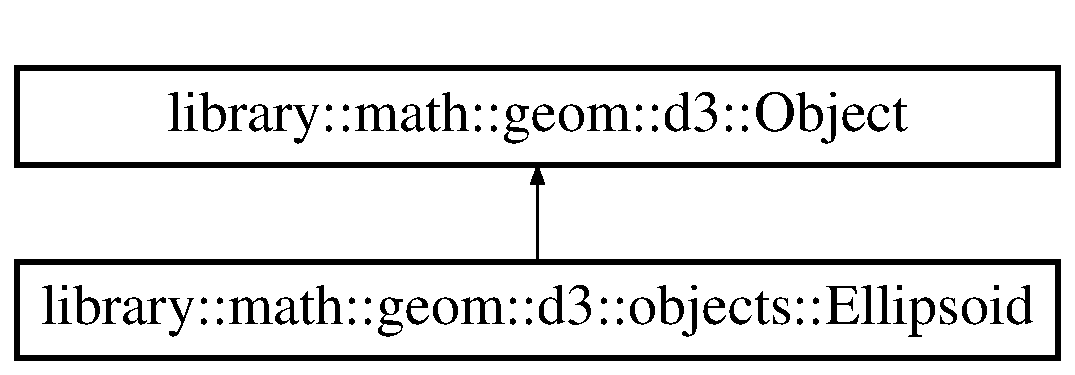
\includegraphics[height=2.000000cm]{classlibrary_1_1math_1_1geom_1_1d3_1_1objects_1_1_ellipsoid}
\end{center}
\end{figure}
\subsection*{Public Member Functions}
\begin{DoxyCompactItemize}
\item 
\hyperlink{classlibrary_1_1math_1_1geom_1_1d3_1_1objects_1_1_ellipsoid_aae81fe0edc7f0e8d4590ea89ae73cb14}{Ellipsoid} (const \hyperlink{classlibrary_1_1math_1_1geom_1_1d3_1_1objects_1_1_point}{Point} \&a\+Center, const Real \&a\+First\+Principal\+Semi\+Axis, const Real \&a\+Second\+Principal\+Semi\+Axis, const Real \&a\+Third\+Principal\+Semi\+Axis, const \hyperlink{classlibrary_1_1math_1_1geom_1_1d3_1_1trf_1_1rot_1_1_quaternion}{Quaternion} \&an\+Orientation=\hyperlink{classlibrary_1_1math_1_1geom_1_1d3_1_1trf_1_1rot_1_1_quaternion_a8076524c66a805b16dffc27efd11e245}{Quaternion\+::\+Unit}())
\begin{DoxyCompactList}\small\item\em Constructor. \end{DoxyCompactList}\item 
virtual \hyperlink{classlibrary_1_1math_1_1geom_1_1d3_1_1objects_1_1_ellipsoid}{Ellipsoid} $\ast$ \hyperlink{classlibrary_1_1math_1_1geom_1_1d3_1_1objects_1_1_ellipsoid_a8982455e000708f1b7e4caf728e7ad40}{clone} () const override
\begin{DoxyCompactList}\small\item\em Clone ellipsoid. \end{DoxyCompactList}\item 
bool \hyperlink{classlibrary_1_1math_1_1geom_1_1d3_1_1objects_1_1_ellipsoid_a259ca94e493d1e8694292aaa579ae1e7}{operator==} (const \hyperlink{classlibrary_1_1math_1_1geom_1_1d3_1_1objects_1_1_ellipsoid}{Ellipsoid} \&an\+Ellipsoid) const
\begin{DoxyCompactList}\small\item\em Equal to operator. \end{DoxyCompactList}\item 
bool \hyperlink{classlibrary_1_1math_1_1geom_1_1d3_1_1objects_1_1_ellipsoid_af6e0b91e6de57a4fa4c027442613d91b}{operator!=} (const \hyperlink{classlibrary_1_1math_1_1geom_1_1d3_1_1objects_1_1_ellipsoid}{Ellipsoid} \&an\+Ellipsoid) const
\begin{DoxyCompactList}\small\item\em Not equal to operator. \end{DoxyCompactList}\item 
virtual bool \hyperlink{classlibrary_1_1math_1_1geom_1_1d3_1_1objects_1_1_ellipsoid_adb42c2c7734c27dcb16d947fc5c9d76d}{is\+Defined} () const override
\begin{DoxyCompactList}\small\item\em Check if ellipsoid is defined. \end{DoxyCompactList}\item 
bool \hyperlink{classlibrary_1_1math_1_1geom_1_1d3_1_1objects_1_1_ellipsoid_ab5fedfe26943a98263bfa441c259581b}{intersects} (const \hyperlink{classlibrary_1_1math_1_1geom_1_1d3_1_1objects_1_1_point}{Point} \&a\+Point) const
\begin{DoxyCompactList}\small\item\em Check if ellipsoid intersects point. \end{DoxyCompactList}\item 
bool \hyperlink{classlibrary_1_1math_1_1geom_1_1d3_1_1objects_1_1_ellipsoid_a2058e665b70c0e883a6ca195fa97120e}{intersects} (const \hyperlink{classlibrary_1_1math_1_1geom_1_1d3_1_1objects_1_1_point_set}{Point\+Set} \&a\+Point\+Set) const
\begin{DoxyCompactList}\small\item\em Check if ellipsoid intersects point set. \end{DoxyCompactList}\item 
bool \hyperlink{classlibrary_1_1math_1_1geom_1_1d3_1_1objects_1_1_ellipsoid_a50957c46fca340a2d20e1845f97f9131}{intersects} (const \hyperlink{classlibrary_1_1math_1_1geom_1_1d3_1_1objects_1_1_line}{Line} \&a\+Line) const
\begin{DoxyCompactList}\small\item\em Check if ellipsoid intersects line. \end{DoxyCompactList}\item 
bool \hyperlink{classlibrary_1_1math_1_1geom_1_1d3_1_1objects_1_1_ellipsoid_a8346f54be39644c22a5a8728ac368832}{intersects} (const \hyperlink{classlibrary_1_1math_1_1geom_1_1d3_1_1objects_1_1_ray}{Ray} \&a\+Ray) const
\begin{DoxyCompactList}\small\item\em Check if ellipsoid intersects ray. \end{DoxyCompactList}\item 
bool \hyperlink{classlibrary_1_1math_1_1geom_1_1d3_1_1objects_1_1_ellipsoid_a6d447b106d193af47c6b201f7e01bd26}{intersects} (const \hyperlink{classlibrary_1_1math_1_1geom_1_1d3_1_1objects_1_1_segment}{Segment} \&a\+Segment) const
\begin{DoxyCompactList}\small\item\em Check if ellipsoid intersects segment. \end{DoxyCompactList}\item 
bool \hyperlink{classlibrary_1_1math_1_1geom_1_1d3_1_1objects_1_1_ellipsoid_ada79a3cf3bf68843a8313eb914c21a95}{intersects} (const \hyperlink{classlibrary_1_1math_1_1geom_1_1d3_1_1objects_1_1_plane}{Plane} \&a\+Plane) const
\begin{DoxyCompactList}\small\item\em Check if ellipsoid intersects plane. \end{DoxyCompactList}\item 
bool \hyperlink{classlibrary_1_1math_1_1geom_1_1d3_1_1objects_1_1_ellipsoid_aa9d3833e3d2be95ff00d7af32fe9b15e}{intersects} (const \hyperlink{classlibrary_1_1math_1_1geom_1_1d3_1_1objects_1_1_sphere}{Sphere} \&a\+Sphere) const
\begin{DoxyCompactList}\small\item\em Check if ellipsoid intersects sphere. \end{DoxyCompactList}\item 
bool \hyperlink{classlibrary_1_1math_1_1geom_1_1d3_1_1objects_1_1_ellipsoid_a4dfd1a3feba0ebed8a5adf89120ce53c}{intersects} (const \hyperlink{classlibrary_1_1math_1_1geom_1_1d3_1_1objects_1_1_ellipsoid}{Ellipsoid} \&an\+Ellipsoid) const
\begin{DoxyCompactList}\small\item\em Check if ellipsoid intersects ellipsoid. \end{DoxyCompactList}\item 
bool \hyperlink{classlibrary_1_1math_1_1geom_1_1d3_1_1objects_1_1_ellipsoid_a05dc13a49a72cb23046ff5735072765b}{intersects} (const \hyperlink{classlibrary_1_1math_1_1geom_1_1d3_1_1objects_1_1_pyramid}{Pyramid} \&a\+Pyramid) const
\begin{DoxyCompactList}\small\item\em Check if ellipsoid intersects pyramid. \end{DoxyCompactList}\item 
bool \hyperlink{classlibrary_1_1math_1_1geom_1_1d3_1_1objects_1_1_ellipsoid_ab48166cd354dbcbc667a11cf6ef19593}{intersects} (const \hyperlink{classlibrary_1_1math_1_1geom_1_1d3_1_1objects_1_1_cone}{Cone} \&a\+Cone) const
\begin{DoxyCompactList}\small\item\em Check if ellipsoid intersects cone. \end{DoxyCompactList}\item 
bool \hyperlink{classlibrary_1_1math_1_1geom_1_1d3_1_1objects_1_1_ellipsoid_ae54cb74c4e6445988ac4d78e00288dd2}{contains} (const \hyperlink{classlibrary_1_1math_1_1geom_1_1d3_1_1objects_1_1_point}{Point} \&a\+Point) const
\begin{DoxyCompactList}\small\item\em Check if ellipsoid contains point. \end{DoxyCompactList}\item 
bool \hyperlink{classlibrary_1_1math_1_1geom_1_1d3_1_1objects_1_1_ellipsoid_af539fe9e2be122e3f994a48e7d308fd0}{contains} (const \hyperlink{classlibrary_1_1math_1_1geom_1_1d3_1_1objects_1_1_point_set}{Point\+Set} \&a\+Point\+Set) const
\begin{DoxyCompactList}\small\item\em Check if ellipsoid contains point set. \end{DoxyCompactList}\item 
bool \hyperlink{classlibrary_1_1math_1_1geom_1_1d3_1_1objects_1_1_ellipsoid_a4b0c41a41fbd8f158da26825f04c47d5}{contains} (const \hyperlink{classlibrary_1_1math_1_1geom_1_1d3_1_1objects_1_1_segment}{Segment} \&a\+Segment) const
\begin{DoxyCompactList}\small\item\em Check if ellipsoid contains segment. \end{DoxyCompactList}\item 
\hyperlink{classlibrary_1_1math_1_1geom_1_1d3_1_1objects_1_1_point}{Point} \hyperlink{classlibrary_1_1math_1_1geom_1_1d3_1_1objects_1_1_ellipsoid_a646be2506950d250db0fb6610979bb46}{get\+Center} () const
\begin{DoxyCompactList}\small\item\em Get ellipsoid center. \end{DoxyCompactList}\item 
Real \hyperlink{classlibrary_1_1math_1_1geom_1_1d3_1_1objects_1_1_ellipsoid_a8219b05b4c6afcd71e915d10b6129baf}{get\+First\+Principal\+Semi\+Axis} () const
\begin{DoxyCompactList}\small\item\em Get ellipsoid first principal semi-\/axis. \end{DoxyCompactList}\item 
Real \hyperlink{classlibrary_1_1math_1_1geom_1_1d3_1_1objects_1_1_ellipsoid_abdc2cc0bed7d473f0d4f572afd0de054}{get\+Second\+Principal\+Semi\+Axis} () const
\begin{DoxyCompactList}\small\item\em Get ellipsoid second principal semi-\/axis. \end{DoxyCompactList}\item 
Real \hyperlink{classlibrary_1_1math_1_1geom_1_1d3_1_1objects_1_1_ellipsoid_a62b97423985083db726d34eced6b58ae}{get\+Third\+Principal\+Semi\+Axis} () const
\begin{DoxyCompactList}\small\item\em Get ellipsoid third principal semi-\/axis. \end{DoxyCompactList}\item 
Vector3d \hyperlink{classlibrary_1_1math_1_1geom_1_1d3_1_1objects_1_1_ellipsoid_a155ca01528d96ae76bfcbb155c832a20}{get\+First\+Axis} () const
\begin{DoxyCompactList}\small\item\em Get ellipsoid first axis. \end{DoxyCompactList}\item 
Vector3d \hyperlink{classlibrary_1_1math_1_1geom_1_1d3_1_1objects_1_1_ellipsoid_a33dde96894c213da77ee116ff18fdf86}{get\+Second\+Axis} () const
\begin{DoxyCompactList}\small\item\em Get ellipsoid second axis. \end{DoxyCompactList}\item 
Vector3d \hyperlink{classlibrary_1_1math_1_1geom_1_1d3_1_1objects_1_1_ellipsoid_a12dc0fd72c672b3d78ec9a286db30c70}{get\+Third\+Axis} () const
\begin{DoxyCompactList}\small\item\em Get ellipsoid third axis. \end{DoxyCompactList}\item 
\hyperlink{classlibrary_1_1math_1_1geom_1_1d3_1_1trf_1_1rot_1_1_quaternion}{Quaternion} \hyperlink{classlibrary_1_1math_1_1geom_1_1d3_1_1objects_1_1_ellipsoid_a8d426da587827eff577de4edb58ae417}{get\+Orientation} () const
\begin{DoxyCompactList}\small\item\em Get ellipsoid orientation. \end{DoxyCompactList}\item 
Matrix3d \hyperlink{classlibrary_1_1math_1_1geom_1_1d3_1_1objects_1_1_ellipsoid_ae6af9f16762e8c38b0a71c306d29ddbf}{get\+Matrix} () const
\begin{DoxyCompactList}\small\item\em Get ellipsoid matrix. \end{DoxyCompactList}\item 
\hyperlink{classlibrary_1_1math_1_1geom_1_1d3_1_1_intersection}{Intersection} \hyperlink{classlibrary_1_1math_1_1geom_1_1d3_1_1objects_1_1_ellipsoid_a5a043a5a0ad0c68771902824c9ea0190}{intersection\+With} (const \hyperlink{classlibrary_1_1math_1_1geom_1_1d3_1_1objects_1_1_line}{Line} \&a\+Line) const
\begin{DoxyCompactList}\small\item\em Compute intersection of ellipsoid with line. \end{DoxyCompactList}\item 
\hyperlink{classlibrary_1_1math_1_1geom_1_1d3_1_1_intersection}{Intersection} \hyperlink{classlibrary_1_1math_1_1geom_1_1d3_1_1objects_1_1_ellipsoid_a2a7c282ac6d4b54210582953e37c8ab5}{intersection\+With} (const \hyperlink{classlibrary_1_1math_1_1geom_1_1d3_1_1objects_1_1_ray}{Ray} \&a\+Ray, const bool only\+In\+Sight=false) const
\begin{DoxyCompactList}\small\item\em Compute intersection of ellipsoid with ray. \end{DoxyCompactList}\item 
\hyperlink{classlibrary_1_1math_1_1geom_1_1d3_1_1_intersection}{Intersection} \hyperlink{classlibrary_1_1math_1_1geom_1_1d3_1_1objects_1_1_ellipsoid_a28ba552ce19297c754a7ca17430c5716}{intersection\+With} (const \hyperlink{classlibrary_1_1math_1_1geom_1_1d3_1_1objects_1_1_segment}{Segment} \&a\+Segment) const
\begin{DoxyCompactList}\small\item\em Compute intersection of ellipsoid with segment. \end{DoxyCompactList}\item 
\hyperlink{classlibrary_1_1math_1_1geom_1_1d3_1_1_intersection}{Intersection} \hyperlink{classlibrary_1_1math_1_1geom_1_1d3_1_1objects_1_1_ellipsoid_a84b3e80768ab52ba5c3b538eda77583c}{intersection\+With} (const \hyperlink{classlibrary_1_1math_1_1geom_1_1d3_1_1objects_1_1_pyramid}{Pyramid} \&a\+Pyramid, const bool only\+In\+Sight=false) const
\begin{DoxyCompactList}\small\item\em Compute intersection of ellipsoid with pyramid. \end{DoxyCompactList}\item 
\hyperlink{classlibrary_1_1math_1_1geom_1_1d3_1_1_intersection}{Intersection} \hyperlink{classlibrary_1_1math_1_1geom_1_1d3_1_1objects_1_1_ellipsoid_a65d88f22d1eb931021ec78eda96055af}{intersection\+With} (const \hyperlink{classlibrary_1_1math_1_1geom_1_1d3_1_1objects_1_1_cone}{Cone} \&a\+Cone, const bool only\+In\+Sight=false) const
\begin{DoxyCompactList}\small\item\em Compute intersection of ellipsoid with cone. \end{DoxyCompactList}\item 
virtual void \hyperlink{classlibrary_1_1math_1_1geom_1_1d3_1_1objects_1_1_ellipsoid_af912ba3948bd06ac517c727210082df3}{print} (std\+::ostream \&an\+Output\+Stream, bool display\+Decorators=true) const override
\begin{DoxyCompactList}\small\item\em Print ellipsoid. \end{DoxyCompactList}\item 
virtual void \hyperlink{classlibrary_1_1math_1_1geom_1_1d3_1_1objects_1_1_ellipsoid_a101408b676b518c0270ebabc55f288d2}{apply\+Transformation} (const \hyperlink{classlibrary_1_1math_1_1geom_1_1d3_1_1_transformation}{Transformation} \&a\+Transformation) override
\begin{DoxyCompactList}\small\item\em Apply transformation to ellipsoid. \end{DoxyCompactList}\end{DoxyCompactItemize}
\subsection*{Static Public Member Functions}
\begin{DoxyCompactItemize}
\item 
static \hyperlink{classlibrary_1_1math_1_1geom_1_1d3_1_1objects_1_1_ellipsoid}{Ellipsoid} \hyperlink{classlibrary_1_1math_1_1geom_1_1d3_1_1objects_1_1_ellipsoid_affcef36f736e6d21a0246a149b8fb688}{Undefined} ()
\begin{DoxyCompactList}\small\item\em Constructs an undefined ellipsoid. \end{DoxyCompactList}\end{DoxyCompactItemize}


\subsection{Detailed Description}
\hyperlink{classlibrary_1_1math_1_1geom_1_1d3_1_1objects_1_1_ellipsoid}{Ellipsoid}. 

https\+://en.wikipedia.\+org/wiki/\+Ellipsoid 

\subsection{Constructor \& Destructor Documentation}
\mbox{\Hypertarget{classlibrary_1_1math_1_1geom_1_1d3_1_1objects_1_1_ellipsoid_aae81fe0edc7f0e8d4590ea89ae73cb14}\label{classlibrary_1_1math_1_1geom_1_1d3_1_1objects_1_1_ellipsoid_aae81fe0edc7f0e8d4590ea89ae73cb14}} 
\index{library\+::math\+::geom\+::d3\+::objects\+::\+Ellipsoid@{library\+::math\+::geom\+::d3\+::objects\+::\+Ellipsoid}!Ellipsoid@{Ellipsoid}}
\index{Ellipsoid@{Ellipsoid}!library\+::math\+::geom\+::d3\+::objects\+::\+Ellipsoid@{library\+::math\+::geom\+::d3\+::objects\+::\+Ellipsoid}}
\subsubsection{\texorpdfstring{Ellipsoid()}{Ellipsoid()}}
{\footnotesize\ttfamily library\+::math\+::geom\+::d3\+::objects\+::\+Ellipsoid\+::\+Ellipsoid (\begin{DoxyParamCaption}\item[{const \hyperlink{classlibrary_1_1math_1_1geom_1_1d3_1_1objects_1_1_point}{Point} \&}]{a\+Center,  }\item[{const Real \&}]{a\+First\+Principal\+Semi\+Axis,  }\item[{const Real \&}]{a\+Second\+Principal\+Semi\+Axis,  }\item[{const Real \&}]{a\+Third\+Principal\+Semi\+Axis,  }\item[{const \hyperlink{classlibrary_1_1math_1_1geom_1_1d3_1_1trf_1_1rot_1_1_quaternion}{Quaternion} \&}]{an\+Orientation = {\ttfamily \hyperlink{classlibrary_1_1math_1_1geom_1_1d3_1_1trf_1_1rot_1_1_quaternion_a8076524c66a805b16dffc27efd11e245}{Quaternion\+::\+Unit}()} }\end{DoxyParamCaption})}



Constructor. 


\begin{DoxyCode}
\hyperlink{classlibrary_1_1math_1_1geom_1_1d3_1_1objects_1_1_ellipsoid_aae81fe0edc7f0e8d4590ea89ae73cb14}{Ellipsoid} ellipsoid(\{ 0.0, 0.0, 0.0 \}, 1.0, 2.0, 3.0) ;
\end{DoxyCode}



\begin{DoxyParams}[1]{Parameters}
\mbox{\tt in}  & {\em a\+Center} & An ellipsoid center \\
\hline
\mbox{\tt in}  & {\em a\+First\+Principal\+Semi\+Axis} & An ellipsoid first principal semi-\/axis \\
\hline
\mbox{\tt in}  & {\em a\+Second\+Principal\+Semi\+Axis} & An ellipsoid second principal semi-\/axis \\
\hline
\mbox{\tt in}  & {\em a\+Third\+Principal\+Semi\+Axis} & An ellipsoid third principal semi-\/axis \\
\hline
\mbox{\tt in}  & {\em (optional)} & an\+Orientation An ellipsoid orientation \\
\hline
\end{DoxyParams}


\subsection{Member Function Documentation}
\mbox{\Hypertarget{classlibrary_1_1math_1_1geom_1_1d3_1_1objects_1_1_ellipsoid_a101408b676b518c0270ebabc55f288d2}\label{classlibrary_1_1math_1_1geom_1_1d3_1_1objects_1_1_ellipsoid_a101408b676b518c0270ebabc55f288d2}} 
\index{library\+::math\+::geom\+::d3\+::objects\+::\+Ellipsoid@{library\+::math\+::geom\+::d3\+::objects\+::\+Ellipsoid}!apply\+Transformation@{apply\+Transformation}}
\index{apply\+Transformation@{apply\+Transformation}!library\+::math\+::geom\+::d3\+::objects\+::\+Ellipsoid@{library\+::math\+::geom\+::d3\+::objects\+::\+Ellipsoid}}
\subsubsection{\texorpdfstring{apply\+Transformation()}{applyTransformation()}}
{\footnotesize\ttfamily void library\+::math\+::geom\+::d3\+::objects\+::\+Ellipsoid\+::apply\+Transformation (\begin{DoxyParamCaption}\item[{const \hyperlink{classlibrary_1_1math_1_1geom_1_1d3_1_1_transformation}{Transformation} \&}]{a\+Transformation }\end{DoxyParamCaption})\hspace{0.3cm}{\ttfamily [override]}, {\ttfamily [virtual]}}



Apply transformation to ellipsoid. 


\begin{DoxyParams}[1]{Parameters}
\mbox{\tt in}  & {\em a\+Transformation} & A transformation \\
\hline
\end{DoxyParams}


Implements \hyperlink{classlibrary_1_1math_1_1geom_1_1d3_1_1_object_a5fc47b1ee5d9a28efc6010d3d1512470}{library\+::math\+::geom\+::d3\+::\+Object}.

\mbox{\Hypertarget{classlibrary_1_1math_1_1geom_1_1d3_1_1objects_1_1_ellipsoid_a8982455e000708f1b7e4caf728e7ad40}\label{classlibrary_1_1math_1_1geom_1_1d3_1_1objects_1_1_ellipsoid_a8982455e000708f1b7e4caf728e7ad40}} 
\index{library\+::math\+::geom\+::d3\+::objects\+::\+Ellipsoid@{library\+::math\+::geom\+::d3\+::objects\+::\+Ellipsoid}!clone@{clone}}
\index{clone@{clone}!library\+::math\+::geom\+::d3\+::objects\+::\+Ellipsoid@{library\+::math\+::geom\+::d3\+::objects\+::\+Ellipsoid}}
\subsubsection{\texorpdfstring{clone()}{clone()}}
{\footnotesize\ttfamily \hyperlink{classlibrary_1_1math_1_1geom_1_1d3_1_1objects_1_1_ellipsoid}{Ellipsoid} $\ast$ library\+::math\+::geom\+::d3\+::objects\+::\+Ellipsoid\+::clone (\begin{DoxyParamCaption}{ }\end{DoxyParamCaption}) const\hspace{0.3cm}{\ttfamily [override]}, {\ttfamily [virtual]}}



Clone ellipsoid. 

\begin{DoxyReturn}{Returns}
Pointer to cloned ellipsoid 
\end{DoxyReturn}


Implements \hyperlink{classlibrary_1_1math_1_1geom_1_1d3_1_1_object_a1a784c6b359e0eb97cd34fabc42f2f3f}{library\+::math\+::geom\+::d3\+::\+Object}.

\mbox{\Hypertarget{classlibrary_1_1math_1_1geom_1_1d3_1_1objects_1_1_ellipsoid_ae54cb74c4e6445988ac4d78e00288dd2}\label{classlibrary_1_1math_1_1geom_1_1d3_1_1objects_1_1_ellipsoid_ae54cb74c4e6445988ac4d78e00288dd2}} 
\index{library\+::math\+::geom\+::d3\+::objects\+::\+Ellipsoid@{library\+::math\+::geom\+::d3\+::objects\+::\+Ellipsoid}!contains@{contains}}
\index{contains@{contains}!library\+::math\+::geom\+::d3\+::objects\+::\+Ellipsoid@{library\+::math\+::geom\+::d3\+::objects\+::\+Ellipsoid}}
\subsubsection{\texorpdfstring{contains()}{contains()}\hspace{0.1cm}{\footnotesize\ttfamily [1/3]}}
{\footnotesize\ttfamily bool library\+::math\+::geom\+::d3\+::objects\+::\+Ellipsoid\+::contains (\begin{DoxyParamCaption}\item[{const \hyperlink{classlibrary_1_1math_1_1geom_1_1d3_1_1objects_1_1_point}{Point} \&}]{a\+Point }\end{DoxyParamCaption}) const}



Check if ellipsoid contains point. 


\begin{DoxyCode}
\hyperlink{classlibrary_1_1math_1_1geom_1_1d3_1_1objects_1_1_ellipsoid_aae81fe0edc7f0e8d4590ea89ae73cb14}{Ellipsoid} ellipsoid = ... ;
Point point = ... ;
ellipsoid.contains(point) ;
\end{DoxyCode}



\begin{DoxyParams}[1]{Parameters}
\mbox{\tt in}  & {\em a\+Point} & A point \\
\hline
\end{DoxyParams}
\begin{DoxyReturn}{Returns}
True if ellipsoid contains point 
\end{DoxyReturn}
\mbox{\Hypertarget{classlibrary_1_1math_1_1geom_1_1d3_1_1objects_1_1_ellipsoid_af539fe9e2be122e3f994a48e7d308fd0}\label{classlibrary_1_1math_1_1geom_1_1d3_1_1objects_1_1_ellipsoid_af539fe9e2be122e3f994a48e7d308fd0}} 
\index{library\+::math\+::geom\+::d3\+::objects\+::\+Ellipsoid@{library\+::math\+::geom\+::d3\+::objects\+::\+Ellipsoid}!contains@{contains}}
\index{contains@{contains}!library\+::math\+::geom\+::d3\+::objects\+::\+Ellipsoid@{library\+::math\+::geom\+::d3\+::objects\+::\+Ellipsoid}}
\subsubsection{\texorpdfstring{contains()}{contains()}\hspace{0.1cm}{\footnotesize\ttfamily [2/3]}}
{\footnotesize\ttfamily bool library\+::math\+::geom\+::d3\+::objects\+::\+Ellipsoid\+::contains (\begin{DoxyParamCaption}\item[{const \hyperlink{classlibrary_1_1math_1_1geom_1_1d3_1_1objects_1_1_point_set}{Point\+Set} \&}]{a\+Point\+Set }\end{DoxyParamCaption}) const}



Check if ellipsoid contains point set. 


\begin{DoxyCode}
\hyperlink{classlibrary_1_1math_1_1geom_1_1d3_1_1objects_1_1_ellipsoid_aae81fe0edc7f0e8d4590ea89ae73cb14}{Ellipsoid} ellipsoid = ... ;
PointSet pointSet = ... ;
ellipsoid.contains(pointSet) ;
\end{DoxyCode}



\begin{DoxyParams}[1]{Parameters}
\mbox{\tt in}  & {\em a\+Point\+Set} & A point set \\
\hline
\end{DoxyParams}
\begin{DoxyReturn}{Returns}
True if ellipsoid contains point set 
\end{DoxyReturn}
\mbox{\Hypertarget{classlibrary_1_1math_1_1geom_1_1d3_1_1objects_1_1_ellipsoid_a4b0c41a41fbd8f158da26825f04c47d5}\label{classlibrary_1_1math_1_1geom_1_1d3_1_1objects_1_1_ellipsoid_a4b0c41a41fbd8f158da26825f04c47d5}} 
\index{library\+::math\+::geom\+::d3\+::objects\+::\+Ellipsoid@{library\+::math\+::geom\+::d3\+::objects\+::\+Ellipsoid}!contains@{contains}}
\index{contains@{contains}!library\+::math\+::geom\+::d3\+::objects\+::\+Ellipsoid@{library\+::math\+::geom\+::d3\+::objects\+::\+Ellipsoid}}
\subsubsection{\texorpdfstring{contains()}{contains()}\hspace{0.1cm}{\footnotesize\ttfamily [3/3]}}
{\footnotesize\ttfamily bool library\+::math\+::geom\+::d3\+::objects\+::\+Ellipsoid\+::contains (\begin{DoxyParamCaption}\item[{const \hyperlink{classlibrary_1_1math_1_1geom_1_1d3_1_1objects_1_1_segment}{Segment} \&}]{a\+Segment }\end{DoxyParamCaption}) const}



Check if ellipsoid contains segment. 


\begin{DoxyCode}
\hyperlink{classlibrary_1_1math_1_1geom_1_1d3_1_1objects_1_1_ellipsoid_aae81fe0edc7f0e8d4590ea89ae73cb14}{Ellipsoid} ellipsoid = ... ;
Segment segment = ... ;
ellipsoid.contains(segment) ;
\end{DoxyCode}



\begin{DoxyParams}[1]{Parameters}
\mbox{\tt in}  & {\em a\+Segment} & A segment \\
\hline
\end{DoxyParams}
\begin{DoxyReturn}{Returns}
True if ellipsoid contains segment 
\end{DoxyReturn}
\mbox{\Hypertarget{classlibrary_1_1math_1_1geom_1_1d3_1_1objects_1_1_ellipsoid_a646be2506950d250db0fb6610979bb46}\label{classlibrary_1_1math_1_1geom_1_1d3_1_1objects_1_1_ellipsoid_a646be2506950d250db0fb6610979bb46}} 
\index{library\+::math\+::geom\+::d3\+::objects\+::\+Ellipsoid@{library\+::math\+::geom\+::d3\+::objects\+::\+Ellipsoid}!get\+Center@{get\+Center}}
\index{get\+Center@{get\+Center}!library\+::math\+::geom\+::d3\+::objects\+::\+Ellipsoid@{library\+::math\+::geom\+::d3\+::objects\+::\+Ellipsoid}}
\subsubsection{\texorpdfstring{get\+Center()}{getCenter()}}
{\footnotesize\ttfamily \hyperlink{classlibrary_1_1math_1_1geom_1_1d3_1_1objects_1_1_point}{Point} library\+::math\+::geom\+::d3\+::objects\+::\+Ellipsoid\+::get\+Center (\begin{DoxyParamCaption}{ }\end{DoxyParamCaption}) const}



Get ellipsoid center. 


\begin{DoxyCode}
\hyperlink{classlibrary_1_1math_1_1geom_1_1d3_1_1objects_1_1_ellipsoid_aae81fe0edc7f0e8d4590ea89ae73cb14}{Ellipsoid}(\hyperlink{classlibrary_1_1math_1_1geom_1_1d3_1_1objects_1_1_point_ab2a38e285c562e50bf350272c083986f}{Point::Origin}(), 1.0, 2.0, 3.0).getCenter() ; \textcolor{comment}{// [0.0, 0.0, 0.0]}
\end{DoxyCode}


\begin{DoxyReturn}{Returns}
\hyperlink{classlibrary_1_1math_1_1geom_1_1d3_1_1objects_1_1_ellipsoid}{Ellipsoid} center 
\end{DoxyReturn}
\mbox{\Hypertarget{classlibrary_1_1math_1_1geom_1_1d3_1_1objects_1_1_ellipsoid_a155ca01528d96ae76bfcbb155c832a20}\label{classlibrary_1_1math_1_1geom_1_1d3_1_1objects_1_1_ellipsoid_a155ca01528d96ae76bfcbb155c832a20}} 
\index{library\+::math\+::geom\+::d3\+::objects\+::\+Ellipsoid@{library\+::math\+::geom\+::d3\+::objects\+::\+Ellipsoid}!get\+First\+Axis@{get\+First\+Axis}}
\index{get\+First\+Axis@{get\+First\+Axis}!library\+::math\+::geom\+::d3\+::objects\+::\+Ellipsoid@{library\+::math\+::geom\+::d3\+::objects\+::\+Ellipsoid}}
\subsubsection{\texorpdfstring{get\+First\+Axis()}{getFirstAxis()}}
{\footnotesize\ttfamily Vector3d library\+::math\+::geom\+::d3\+::objects\+::\+Ellipsoid\+::get\+First\+Axis (\begin{DoxyParamCaption}{ }\end{DoxyParamCaption}) const}



Get ellipsoid first axis. 

\begin{DoxyReturn}{Returns}
\hyperlink{classlibrary_1_1math_1_1geom_1_1d3_1_1objects_1_1_ellipsoid}{Ellipsoid} first axis 
\end{DoxyReturn}
\mbox{\Hypertarget{classlibrary_1_1math_1_1geom_1_1d3_1_1objects_1_1_ellipsoid_a8219b05b4c6afcd71e915d10b6129baf}\label{classlibrary_1_1math_1_1geom_1_1d3_1_1objects_1_1_ellipsoid_a8219b05b4c6afcd71e915d10b6129baf}} 
\index{library\+::math\+::geom\+::d3\+::objects\+::\+Ellipsoid@{library\+::math\+::geom\+::d3\+::objects\+::\+Ellipsoid}!get\+First\+Principal\+Semi\+Axis@{get\+First\+Principal\+Semi\+Axis}}
\index{get\+First\+Principal\+Semi\+Axis@{get\+First\+Principal\+Semi\+Axis}!library\+::math\+::geom\+::d3\+::objects\+::\+Ellipsoid@{library\+::math\+::geom\+::d3\+::objects\+::\+Ellipsoid}}
\subsubsection{\texorpdfstring{get\+First\+Principal\+Semi\+Axis()}{getFirstPrincipalSemiAxis()}}
{\footnotesize\ttfamily Real library\+::math\+::geom\+::d3\+::objects\+::\+Ellipsoid\+::get\+First\+Principal\+Semi\+Axis (\begin{DoxyParamCaption}{ }\end{DoxyParamCaption}) const}



Get ellipsoid first principal semi-\/axis. 


\begin{DoxyCode}
\hyperlink{classlibrary_1_1math_1_1geom_1_1d3_1_1objects_1_1_ellipsoid_aae81fe0edc7f0e8d4590ea89ae73cb14}{Ellipsoid}(\hyperlink{classlibrary_1_1math_1_1geom_1_1d3_1_1objects_1_1_point_ab2a38e285c562e50bf350272c083986f}{Point::Origin}(), 1.0, 2.0, 3.0).getFirstPrincipalSemiAxis() ; \textcolor{comment}{// 1.0}
\end{DoxyCode}


\begin{DoxyReturn}{Returns}
\hyperlink{classlibrary_1_1math_1_1geom_1_1d3_1_1objects_1_1_ellipsoid}{Ellipsoid} first principal semi-\/axis 
\end{DoxyReturn}
\mbox{\Hypertarget{classlibrary_1_1math_1_1geom_1_1d3_1_1objects_1_1_ellipsoid_ae6af9f16762e8c38b0a71c306d29ddbf}\label{classlibrary_1_1math_1_1geom_1_1d3_1_1objects_1_1_ellipsoid_ae6af9f16762e8c38b0a71c306d29ddbf}} 
\index{library\+::math\+::geom\+::d3\+::objects\+::\+Ellipsoid@{library\+::math\+::geom\+::d3\+::objects\+::\+Ellipsoid}!get\+Matrix@{get\+Matrix}}
\index{get\+Matrix@{get\+Matrix}!library\+::math\+::geom\+::d3\+::objects\+::\+Ellipsoid@{library\+::math\+::geom\+::d3\+::objects\+::\+Ellipsoid}}
\subsubsection{\texorpdfstring{get\+Matrix()}{getMatrix()}}
{\footnotesize\ttfamily Matrix3d library\+::math\+::geom\+::d3\+::objects\+::\+Ellipsoid\+::get\+Matrix (\begin{DoxyParamCaption}{ }\end{DoxyParamCaption}) const}



Get ellipsoid matrix. 


\begin{DoxyCode}
\hyperlink{classlibrary_1_1math_1_1geom_1_1d3_1_1objects_1_1_ellipsoid_aae81fe0edc7f0e8d4590ea89ae73cb14}{Ellipsoid}(\hyperlink{classlibrary_1_1math_1_1geom_1_1d3_1_1objects_1_1_point_ab2a38e285c562e50bf350272c083986f}{Point::Origin}(), 1.0, 2.0, 3.0, \hyperlink{classlibrary_1_1math_1_1geom_1_1d3_1_1trf_1_1rot_1_1_quaternion_a006294eb483bcfc352c2dc36cf19ceec}{Quaternion::XYZS}(0.0, 0.0, 
      0.0, 1.0)).getMatrix() ;
\end{DoxyCode}


\begin{DoxyReturn}{Returns}
\hyperlink{classlibrary_1_1math_1_1geom_1_1d3_1_1objects_1_1_ellipsoid}{Ellipsoid} matrix 
\end{DoxyReturn}
\mbox{\Hypertarget{classlibrary_1_1math_1_1geom_1_1d3_1_1objects_1_1_ellipsoid_a8d426da587827eff577de4edb58ae417}\label{classlibrary_1_1math_1_1geom_1_1d3_1_1objects_1_1_ellipsoid_a8d426da587827eff577de4edb58ae417}} 
\index{library\+::math\+::geom\+::d3\+::objects\+::\+Ellipsoid@{library\+::math\+::geom\+::d3\+::objects\+::\+Ellipsoid}!get\+Orientation@{get\+Orientation}}
\index{get\+Orientation@{get\+Orientation}!library\+::math\+::geom\+::d3\+::objects\+::\+Ellipsoid@{library\+::math\+::geom\+::d3\+::objects\+::\+Ellipsoid}}
\subsubsection{\texorpdfstring{get\+Orientation()}{getOrientation()}}
{\footnotesize\ttfamily \hyperlink{classlibrary_1_1math_1_1geom_1_1d3_1_1trf_1_1rot_1_1_quaternion}{Quaternion} library\+::math\+::geom\+::d3\+::objects\+::\+Ellipsoid\+::get\+Orientation (\begin{DoxyParamCaption}{ }\end{DoxyParamCaption}) const}



Get ellipsoid orientation. 


\begin{DoxyCode}
\hyperlink{classlibrary_1_1math_1_1geom_1_1d3_1_1objects_1_1_ellipsoid_aae81fe0edc7f0e8d4590ea89ae73cb14}{Ellipsoid}(\hyperlink{classlibrary_1_1math_1_1geom_1_1d3_1_1objects_1_1_point_ab2a38e285c562e50bf350272c083986f}{Point::Origin}(), 1.0, 2.0, 3.0, \hyperlink{classlibrary_1_1math_1_1geom_1_1d3_1_1trf_1_1rot_1_1_quaternion_a006294eb483bcfc352c2dc36cf19ceec}{Quaternion::XYZS}(0.0, 0.0, 
      0.0, 1.0)).getOrientation() ; \textcolor{comment}{// Quaternion::XYZS(0.0, 0.0, 0.0, 1.0)}
\end{DoxyCode}


\begin{DoxyReturn}{Returns}
\hyperlink{classlibrary_1_1math_1_1geom_1_1d3_1_1objects_1_1_ellipsoid}{Ellipsoid} orientation 
\end{DoxyReturn}
\mbox{\Hypertarget{classlibrary_1_1math_1_1geom_1_1d3_1_1objects_1_1_ellipsoid_a33dde96894c213da77ee116ff18fdf86}\label{classlibrary_1_1math_1_1geom_1_1d3_1_1objects_1_1_ellipsoid_a33dde96894c213da77ee116ff18fdf86}} 
\index{library\+::math\+::geom\+::d3\+::objects\+::\+Ellipsoid@{library\+::math\+::geom\+::d3\+::objects\+::\+Ellipsoid}!get\+Second\+Axis@{get\+Second\+Axis}}
\index{get\+Second\+Axis@{get\+Second\+Axis}!library\+::math\+::geom\+::d3\+::objects\+::\+Ellipsoid@{library\+::math\+::geom\+::d3\+::objects\+::\+Ellipsoid}}
\subsubsection{\texorpdfstring{get\+Second\+Axis()}{getSecondAxis()}}
{\footnotesize\ttfamily Vector3d library\+::math\+::geom\+::d3\+::objects\+::\+Ellipsoid\+::get\+Second\+Axis (\begin{DoxyParamCaption}{ }\end{DoxyParamCaption}) const}



Get ellipsoid second axis. 

\begin{DoxyReturn}{Returns}
\hyperlink{classlibrary_1_1math_1_1geom_1_1d3_1_1objects_1_1_ellipsoid}{Ellipsoid} second axis 
\end{DoxyReturn}
\mbox{\Hypertarget{classlibrary_1_1math_1_1geom_1_1d3_1_1objects_1_1_ellipsoid_abdc2cc0bed7d473f0d4f572afd0de054}\label{classlibrary_1_1math_1_1geom_1_1d3_1_1objects_1_1_ellipsoid_abdc2cc0bed7d473f0d4f572afd0de054}} 
\index{library\+::math\+::geom\+::d3\+::objects\+::\+Ellipsoid@{library\+::math\+::geom\+::d3\+::objects\+::\+Ellipsoid}!get\+Second\+Principal\+Semi\+Axis@{get\+Second\+Principal\+Semi\+Axis}}
\index{get\+Second\+Principal\+Semi\+Axis@{get\+Second\+Principal\+Semi\+Axis}!library\+::math\+::geom\+::d3\+::objects\+::\+Ellipsoid@{library\+::math\+::geom\+::d3\+::objects\+::\+Ellipsoid}}
\subsubsection{\texorpdfstring{get\+Second\+Principal\+Semi\+Axis()}{getSecondPrincipalSemiAxis()}}
{\footnotesize\ttfamily Real library\+::math\+::geom\+::d3\+::objects\+::\+Ellipsoid\+::get\+Second\+Principal\+Semi\+Axis (\begin{DoxyParamCaption}{ }\end{DoxyParamCaption}) const}



Get ellipsoid second principal semi-\/axis. 


\begin{DoxyCode}
\hyperlink{classlibrary_1_1math_1_1geom_1_1d3_1_1objects_1_1_ellipsoid_aae81fe0edc7f0e8d4590ea89ae73cb14}{Ellipsoid}(\hyperlink{classlibrary_1_1math_1_1geom_1_1d3_1_1objects_1_1_point_ab2a38e285c562e50bf350272c083986f}{Point::Origin}(), 1.0, 2.0, 3.0).getSecondPrincipalSemiAxis() ; \textcolor{comment}{// 2.0}
\end{DoxyCode}


\begin{DoxyReturn}{Returns}
\hyperlink{classlibrary_1_1math_1_1geom_1_1d3_1_1objects_1_1_ellipsoid}{Ellipsoid} second principal semi-\/axis 
\end{DoxyReturn}
\mbox{\Hypertarget{classlibrary_1_1math_1_1geom_1_1d3_1_1objects_1_1_ellipsoid_a12dc0fd72c672b3d78ec9a286db30c70}\label{classlibrary_1_1math_1_1geom_1_1d3_1_1objects_1_1_ellipsoid_a12dc0fd72c672b3d78ec9a286db30c70}} 
\index{library\+::math\+::geom\+::d3\+::objects\+::\+Ellipsoid@{library\+::math\+::geom\+::d3\+::objects\+::\+Ellipsoid}!get\+Third\+Axis@{get\+Third\+Axis}}
\index{get\+Third\+Axis@{get\+Third\+Axis}!library\+::math\+::geom\+::d3\+::objects\+::\+Ellipsoid@{library\+::math\+::geom\+::d3\+::objects\+::\+Ellipsoid}}
\subsubsection{\texorpdfstring{get\+Third\+Axis()}{getThirdAxis()}}
{\footnotesize\ttfamily Vector3d library\+::math\+::geom\+::d3\+::objects\+::\+Ellipsoid\+::get\+Third\+Axis (\begin{DoxyParamCaption}{ }\end{DoxyParamCaption}) const}



Get ellipsoid third axis. 

\begin{DoxyReturn}{Returns}
\hyperlink{classlibrary_1_1math_1_1geom_1_1d3_1_1objects_1_1_ellipsoid}{Ellipsoid} third axis 
\end{DoxyReturn}
\mbox{\Hypertarget{classlibrary_1_1math_1_1geom_1_1d3_1_1objects_1_1_ellipsoid_a62b97423985083db726d34eced6b58ae}\label{classlibrary_1_1math_1_1geom_1_1d3_1_1objects_1_1_ellipsoid_a62b97423985083db726d34eced6b58ae}} 
\index{library\+::math\+::geom\+::d3\+::objects\+::\+Ellipsoid@{library\+::math\+::geom\+::d3\+::objects\+::\+Ellipsoid}!get\+Third\+Principal\+Semi\+Axis@{get\+Third\+Principal\+Semi\+Axis}}
\index{get\+Third\+Principal\+Semi\+Axis@{get\+Third\+Principal\+Semi\+Axis}!library\+::math\+::geom\+::d3\+::objects\+::\+Ellipsoid@{library\+::math\+::geom\+::d3\+::objects\+::\+Ellipsoid}}
\subsubsection{\texorpdfstring{get\+Third\+Principal\+Semi\+Axis()}{getThirdPrincipalSemiAxis()}}
{\footnotesize\ttfamily Real library\+::math\+::geom\+::d3\+::objects\+::\+Ellipsoid\+::get\+Third\+Principal\+Semi\+Axis (\begin{DoxyParamCaption}{ }\end{DoxyParamCaption}) const}



Get ellipsoid third principal semi-\/axis. 


\begin{DoxyCode}
\hyperlink{classlibrary_1_1math_1_1geom_1_1d3_1_1objects_1_1_ellipsoid_aae81fe0edc7f0e8d4590ea89ae73cb14}{Ellipsoid}(\hyperlink{classlibrary_1_1math_1_1geom_1_1d3_1_1objects_1_1_point_ab2a38e285c562e50bf350272c083986f}{Point::Origin}(), 1.0, 2.0, 3.0).getThirdPrincipalSemiAxis() ; \textcolor{comment}{// 3.0}
\end{DoxyCode}


\begin{DoxyReturn}{Returns}
\hyperlink{classlibrary_1_1math_1_1geom_1_1d3_1_1objects_1_1_ellipsoid}{Ellipsoid} third principal semi-\/axis 
\end{DoxyReturn}
\mbox{\Hypertarget{classlibrary_1_1math_1_1geom_1_1d3_1_1objects_1_1_ellipsoid_a5a043a5a0ad0c68771902824c9ea0190}\label{classlibrary_1_1math_1_1geom_1_1d3_1_1objects_1_1_ellipsoid_a5a043a5a0ad0c68771902824c9ea0190}} 
\index{library\+::math\+::geom\+::d3\+::objects\+::\+Ellipsoid@{library\+::math\+::geom\+::d3\+::objects\+::\+Ellipsoid}!intersection\+With@{intersection\+With}}
\index{intersection\+With@{intersection\+With}!library\+::math\+::geom\+::d3\+::objects\+::\+Ellipsoid@{library\+::math\+::geom\+::d3\+::objects\+::\+Ellipsoid}}
\subsubsection{\texorpdfstring{intersection\+With()}{intersectionWith()}\hspace{0.1cm}{\footnotesize\ttfamily [1/5]}}
{\footnotesize\ttfamily \hyperlink{classlibrary_1_1math_1_1geom_1_1d3_1_1_intersection}{Intersection} library\+::math\+::geom\+::d3\+::objects\+::\+Ellipsoid\+::intersection\+With (\begin{DoxyParamCaption}\item[{const \hyperlink{classlibrary_1_1math_1_1geom_1_1d3_1_1objects_1_1_line}{Line} \&}]{a\+Line }\end{DoxyParamCaption}) const}



Compute intersection of ellipsoid with line. 


\begin{DoxyParams}[1]{Parameters}
\mbox{\tt in}  & {\em a\+Line} & A line \\
\hline
\end{DoxyParams}
\begin{DoxyReturn}{Returns}
\hyperlink{classlibrary_1_1math_1_1geom_1_1d3_1_1_intersection}{Intersection} of ellipsoid with line 
\end{DoxyReturn}
\mbox{\Hypertarget{classlibrary_1_1math_1_1geom_1_1d3_1_1objects_1_1_ellipsoid_a2a7c282ac6d4b54210582953e37c8ab5}\label{classlibrary_1_1math_1_1geom_1_1d3_1_1objects_1_1_ellipsoid_a2a7c282ac6d4b54210582953e37c8ab5}} 
\index{library\+::math\+::geom\+::d3\+::objects\+::\+Ellipsoid@{library\+::math\+::geom\+::d3\+::objects\+::\+Ellipsoid}!intersection\+With@{intersection\+With}}
\index{intersection\+With@{intersection\+With}!library\+::math\+::geom\+::d3\+::objects\+::\+Ellipsoid@{library\+::math\+::geom\+::d3\+::objects\+::\+Ellipsoid}}
\subsubsection{\texorpdfstring{intersection\+With()}{intersectionWith()}\hspace{0.1cm}{\footnotesize\ttfamily [2/5]}}
{\footnotesize\ttfamily \hyperlink{classlibrary_1_1math_1_1geom_1_1d3_1_1_intersection}{Intersection} library\+::math\+::geom\+::d3\+::objects\+::\+Ellipsoid\+::intersection\+With (\begin{DoxyParamCaption}\item[{const \hyperlink{classlibrary_1_1math_1_1geom_1_1d3_1_1objects_1_1_ray}{Ray} \&}]{a\+Ray,  }\item[{const bool}]{only\+In\+Sight = {\ttfamily false} }\end{DoxyParamCaption}) const}



Compute intersection of ellipsoid with ray. 


\begin{DoxyParams}[1]{Parameters}
\mbox{\tt in}  & {\em a\+Ray} & A ray \\
\hline
\mbox{\tt in}  & {\em only\+In\+Sight} & (optional) If true, only return intersection points that are in sight \\
\hline
\end{DoxyParams}
\begin{DoxyReturn}{Returns}
\hyperlink{classlibrary_1_1math_1_1geom_1_1d3_1_1_intersection}{Intersection} of ellipsoid with ray 
\end{DoxyReturn}
\mbox{\Hypertarget{classlibrary_1_1math_1_1geom_1_1d3_1_1objects_1_1_ellipsoid_a28ba552ce19297c754a7ca17430c5716}\label{classlibrary_1_1math_1_1geom_1_1d3_1_1objects_1_1_ellipsoid_a28ba552ce19297c754a7ca17430c5716}} 
\index{library\+::math\+::geom\+::d3\+::objects\+::\+Ellipsoid@{library\+::math\+::geom\+::d3\+::objects\+::\+Ellipsoid}!intersection\+With@{intersection\+With}}
\index{intersection\+With@{intersection\+With}!library\+::math\+::geom\+::d3\+::objects\+::\+Ellipsoid@{library\+::math\+::geom\+::d3\+::objects\+::\+Ellipsoid}}
\subsubsection{\texorpdfstring{intersection\+With()}{intersectionWith()}\hspace{0.1cm}{\footnotesize\ttfamily [3/5]}}
{\footnotesize\ttfamily \hyperlink{classlibrary_1_1math_1_1geom_1_1d3_1_1_intersection}{Intersection} library\+::math\+::geom\+::d3\+::objects\+::\+Ellipsoid\+::intersection\+With (\begin{DoxyParamCaption}\item[{const \hyperlink{classlibrary_1_1math_1_1geom_1_1d3_1_1objects_1_1_segment}{Segment} \&}]{a\+Segment }\end{DoxyParamCaption}) const}



Compute intersection of ellipsoid with segment. 


\begin{DoxyParams}[1]{Parameters}
\mbox{\tt in}  & {\em a\+Segment} & A segment \\
\hline
\end{DoxyParams}
\begin{DoxyReturn}{Returns}
\hyperlink{classlibrary_1_1math_1_1geom_1_1d3_1_1_intersection}{Intersection} of ellipsoid with segment 
\end{DoxyReturn}
\mbox{\Hypertarget{classlibrary_1_1math_1_1geom_1_1d3_1_1objects_1_1_ellipsoid_a84b3e80768ab52ba5c3b538eda77583c}\label{classlibrary_1_1math_1_1geom_1_1d3_1_1objects_1_1_ellipsoid_a84b3e80768ab52ba5c3b538eda77583c}} 
\index{library\+::math\+::geom\+::d3\+::objects\+::\+Ellipsoid@{library\+::math\+::geom\+::d3\+::objects\+::\+Ellipsoid}!intersection\+With@{intersection\+With}}
\index{intersection\+With@{intersection\+With}!library\+::math\+::geom\+::d3\+::objects\+::\+Ellipsoid@{library\+::math\+::geom\+::d3\+::objects\+::\+Ellipsoid}}
\subsubsection{\texorpdfstring{intersection\+With()}{intersectionWith()}\hspace{0.1cm}{\footnotesize\ttfamily [4/5]}}
{\footnotesize\ttfamily \hyperlink{classlibrary_1_1math_1_1geom_1_1d3_1_1_intersection}{Intersection} library\+::math\+::geom\+::d3\+::objects\+::\+Ellipsoid\+::intersection\+With (\begin{DoxyParamCaption}\item[{const \hyperlink{classlibrary_1_1math_1_1geom_1_1d3_1_1objects_1_1_pyramid}{Pyramid} \&}]{a\+Pyramid,  }\item[{const bool}]{only\+In\+Sight = {\ttfamily false} }\end{DoxyParamCaption}) const}



Compute intersection of ellipsoid with pyramid. 


\begin{DoxyParams}[1]{Parameters}
\mbox{\tt in}  & {\em a\+Pyramid} & A pyramid \\
\hline
\mbox{\tt in}  & {\em only\+In\+Sight} & (optional) If true, only return intersection points that are in sight \\
\hline
\end{DoxyParams}
\begin{DoxyReturn}{Returns}
\hyperlink{classlibrary_1_1math_1_1geom_1_1d3_1_1_intersection}{Intersection} of ellipsoid with pyramid 
\end{DoxyReturn}
\mbox{\Hypertarget{classlibrary_1_1math_1_1geom_1_1d3_1_1objects_1_1_ellipsoid_a65d88f22d1eb931021ec78eda96055af}\label{classlibrary_1_1math_1_1geom_1_1d3_1_1objects_1_1_ellipsoid_a65d88f22d1eb931021ec78eda96055af}} 
\index{library\+::math\+::geom\+::d3\+::objects\+::\+Ellipsoid@{library\+::math\+::geom\+::d3\+::objects\+::\+Ellipsoid}!intersection\+With@{intersection\+With}}
\index{intersection\+With@{intersection\+With}!library\+::math\+::geom\+::d3\+::objects\+::\+Ellipsoid@{library\+::math\+::geom\+::d3\+::objects\+::\+Ellipsoid}}
\subsubsection{\texorpdfstring{intersection\+With()}{intersectionWith()}\hspace{0.1cm}{\footnotesize\ttfamily [5/5]}}
{\footnotesize\ttfamily \hyperlink{classlibrary_1_1math_1_1geom_1_1d3_1_1_intersection}{Intersection} library\+::math\+::geom\+::d3\+::objects\+::\+Ellipsoid\+::intersection\+With (\begin{DoxyParamCaption}\item[{const \hyperlink{classlibrary_1_1math_1_1geom_1_1d3_1_1objects_1_1_cone}{Cone} \&}]{a\+Cone,  }\item[{const bool}]{only\+In\+Sight = {\ttfamily false} }\end{DoxyParamCaption}) const}



Compute intersection of ellipsoid with cone. 


\begin{DoxyParams}[1]{Parameters}
\mbox{\tt in}  & {\em a\+Cone} & A cone \\
\hline
\mbox{\tt in}  & {\em only\+In\+Sight} & (optional) If true, only return intersection points that are in sight \\
\hline
\end{DoxyParams}
\begin{DoxyReturn}{Returns}
\hyperlink{classlibrary_1_1math_1_1geom_1_1d3_1_1_intersection}{Intersection} of ellipsoid with cone 
\end{DoxyReturn}
\mbox{\Hypertarget{classlibrary_1_1math_1_1geom_1_1d3_1_1objects_1_1_ellipsoid_ab5fedfe26943a98263bfa441c259581b}\label{classlibrary_1_1math_1_1geom_1_1d3_1_1objects_1_1_ellipsoid_ab5fedfe26943a98263bfa441c259581b}} 
\index{library\+::math\+::geom\+::d3\+::objects\+::\+Ellipsoid@{library\+::math\+::geom\+::d3\+::objects\+::\+Ellipsoid}!intersects@{intersects}}
\index{intersects@{intersects}!library\+::math\+::geom\+::d3\+::objects\+::\+Ellipsoid@{library\+::math\+::geom\+::d3\+::objects\+::\+Ellipsoid}}
\subsubsection{\texorpdfstring{intersects()}{intersects()}\hspace{0.1cm}{\footnotesize\ttfamily [1/10]}}
{\footnotesize\ttfamily bool library\+::math\+::geom\+::d3\+::objects\+::\+Ellipsoid\+::intersects (\begin{DoxyParamCaption}\item[{const \hyperlink{classlibrary_1_1math_1_1geom_1_1d3_1_1objects_1_1_point}{Point} \&}]{a\+Point }\end{DoxyParamCaption}) const}



Check if ellipsoid intersects point. 


\begin{DoxyCode}
\hyperlink{classlibrary_1_1math_1_1geom_1_1d3_1_1objects_1_1_ellipsoid_aae81fe0edc7f0e8d4590ea89ae73cb14}{Ellipsoid} ellipsoid = ... ;
Point point = ... ;
ellipsoid.intersects(point) ;
\end{DoxyCode}



\begin{DoxyParams}[1]{Parameters}
\mbox{\tt in}  & {\em a\+Point} & A point \\
\hline
\end{DoxyParams}
\begin{DoxyReturn}{Returns}
True if ellipsoid intersects point 
\end{DoxyReturn}
\mbox{\Hypertarget{classlibrary_1_1math_1_1geom_1_1d3_1_1objects_1_1_ellipsoid_a2058e665b70c0e883a6ca195fa97120e}\label{classlibrary_1_1math_1_1geom_1_1d3_1_1objects_1_1_ellipsoid_a2058e665b70c0e883a6ca195fa97120e}} 
\index{library\+::math\+::geom\+::d3\+::objects\+::\+Ellipsoid@{library\+::math\+::geom\+::d3\+::objects\+::\+Ellipsoid}!intersects@{intersects}}
\index{intersects@{intersects}!library\+::math\+::geom\+::d3\+::objects\+::\+Ellipsoid@{library\+::math\+::geom\+::d3\+::objects\+::\+Ellipsoid}}
\subsubsection{\texorpdfstring{intersects()}{intersects()}\hspace{0.1cm}{\footnotesize\ttfamily [2/10]}}
{\footnotesize\ttfamily bool library\+::math\+::geom\+::d3\+::objects\+::\+Ellipsoid\+::intersects (\begin{DoxyParamCaption}\item[{const \hyperlink{classlibrary_1_1math_1_1geom_1_1d3_1_1objects_1_1_point_set}{Point\+Set} \&}]{a\+Point\+Set }\end{DoxyParamCaption}) const}



Check if ellipsoid intersects point set. 


\begin{DoxyCode}
\hyperlink{classlibrary_1_1math_1_1geom_1_1d3_1_1objects_1_1_ellipsoid_aae81fe0edc7f0e8d4590ea89ae73cb14}{Ellipsoid} ellipsoid = ... ;
PointSet pointSet = ... ;
ellipsoid.intersects(pointSet) ;
\end{DoxyCode}



\begin{DoxyParams}[1]{Parameters}
\mbox{\tt in}  & {\em a\+Point\+Set} & A point set \\
\hline
\end{DoxyParams}
\begin{DoxyReturn}{Returns}
True if ellipsoid intersects point set 
\end{DoxyReturn}
\mbox{\Hypertarget{classlibrary_1_1math_1_1geom_1_1d3_1_1objects_1_1_ellipsoid_a50957c46fca340a2d20e1845f97f9131}\label{classlibrary_1_1math_1_1geom_1_1d3_1_1objects_1_1_ellipsoid_a50957c46fca340a2d20e1845f97f9131}} 
\index{library\+::math\+::geom\+::d3\+::objects\+::\+Ellipsoid@{library\+::math\+::geom\+::d3\+::objects\+::\+Ellipsoid}!intersects@{intersects}}
\index{intersects@{intersects}!library\+::math\+::geom\+::d3\+::objects\+::\+Ellipsoid@{library\+::math\+::geom\+::d3\+::objects\+::\+Ellipsoid}}
\subsubsection{\texorpdfstring{intersects()}{intersects()}\hspace{0.1cm}{\footnotesize\ttfamily [3/10]}}
{\footnotesize\ttfamily bool library\+::math\+::geom\+::d3\+::objects\+::\+Ellipsoid\+::intersects (\begin{DoxyParamCaption}\item[{const \hyperlink{classlibrary_1_1math_1_1geom_1_1d3_1_1objects_1_1_line}{Line} \&}]{a\+Line }\end{DoxyParamCaption}) const}



Check if ellipsoid intersects line. 


\begin{DoxyCode}
\hyperlink{classlibrary_1_1math_1_1geom_1_1d3_1_1objects_1_1_ellipsoid_aae81fe0edc7f0e8d4590ea89ae73cb14}{Ellipsoid} ellipsoid = ... ;
Line line = ... ;
ellipsoid.intersects(line) ;
\end{DoxyCode}



\begin{DoxyParams}[1]{Parameters}
\mbox{\tt in}  & {\em a\+Line} & A line \\
\hline
\end{DoxyParams}
\begin{DoxyReturn}{Returns}
True if ellipsoid intersects line 
\end{DoxyReturn}
\mbox{\Hypertarget{classlibrary_1_1math_1_1geom_1_1d3_1_1objects_1_1_ellipsoid_a8346f54be39644c22a5a8728ac368832}\label{classlibrary_1_1math_1_1geom_1_1d3_1_1objects_1_1_ellipsoid_a8346f54be39644c22a5a8728ac368832}} 
\index{library\+::math\+::geom\+::d3\+::objects\+::\+Ellipsoid@{library\+::math\+::geom\+::d3\+::objects\+::\+Ellipsoid}!intersects@{intersects}}
\index{intersects@{intersects}!library\+::math\+::geom\+::d3\+::objects\+::\+Ellipsoid@{library\+::math\+::geom\+::d3\+::objects\+::\+Ellipsoid}}
\subsubsection{\texorpdfstring{intersects()}{intersects()}\hspace{0.1cm}{\footnotesize\ttfamily [4/10]}}
{\footnotesize\ttfamily bool library\+::math\+::geom\+::d3\+::objects\+::\+Ellipsoid\+::intersects (\begin{DoxyParamCaption}\item[{const \hyperlink{classlibrary_1_1math_1_1geom_1_1d3_1_1objects_1_1_ray}{Ray} \&}]{a\+Ray }\end{DoxyParamCaption}) const}



Check if ellipsoid intersects ray. 


\begin{DoxyCode}
\hyperlink{classlibrary_1_1math_1_1geom_1_1d3_1_1objects_1_1_ellipsoid_aae81fe0edc7f0e8d4590ea89ae73cb14}{Ellipsoid} ellipsoid = ... ;
Ray ray = ... ;
ellipsoid.intersects(ray) ;
\end{DoxyCode}



\begin{DoxyParams}[1]{Parameters}
\mbox{\tt in}  & {\em a\+Ray} & A ray \\
\hline
\end{DoxyParams}
\begin{DoxyReturn}{Returns}
True if ellipsoid intersects ray 
\end{DoxyReturn}
\mbox{\Hypertarget{classlibrary_1_1math_1_1geom_1_1d3_1_1objects_1_1_ellipsoid_a6d447b106d193af47c6b201f7e01bd26}\label{classlibrary_1_1math_1_1geom_1_1d3_1_1objects_1_1_ellipsoid_a6d447b106d193af47c6b201f7e01bd26}} 
\index{library\+::math\+::geom\+::d3\+::objects\+::\+Ellipsoid@{library\+::math\+::geom\+::d3\+::objects\+::\+Ellipsoid}!intersects@{intersects}}
\index{intersects@{intersects}!library\+::math\+::geom\+::d3\+::objects\+::\+Ellipsoid@{library\+::math\+::geom\+::d3\+::objects\+::\+Ellipsoid}}
\subsubsection{\texorpdfstring{intersects()}{intersects()}\hspace{0.1cm}{\footnotesize\ttfamily [5/10]}}
{\footnotesize\ttfamily bool library\+::math\+::geom\+::d3\+::objects\+::\+Ellipsoid\+::intersects (\begin{DoxyParamCaption}\item[{const \hyperlink{classlibrary_1_1math_1_1geom_1_1d3_1_1objects_1_1_segment}{Segment} \&}]{a\+Segment }\end{DoxyParamCaption}) const}



Check if ellipsoid intersects segment. 


\begin{DoxyCode}
\hyperlink{classlibrary_1_1math_1_1geom_1_1d3_1_1objects_1_1_ellipsoid_aae81fe0edc7f0e8d4590ea89ae73cb14}{Ellipsoid} ellipsoid = ... ;
Segment segment = ... ;
ellipsoid.intersects(segment) ;
\end{DoxyCode}



\begin{DoxyParams}[1]{Parameters}
\mbox{\tt in}  & {\em a\+Segment} & A segment \\
\hline
\end{DoxyParams}
\begin{DoxyReturn}{Returns}
True if ellipsoid intersects segment 
\end{DoxyReturn}
\mbox{\Hypertarget{classlibrary_1_1math_1_1geom_1_1d3_1_1objects_1_1_ellipsoid_ada79a3cf3bf68843a8313eb914c21a95}\label{classlibrary_1_1math_1_1geom_1_1d3_1_1objects_1_1_ellipsoid_ada79a3cf3bf68843a8313eb914c21a95}} 
\index{library\+::math\+::geom\+::d3\+::objects\+::\+Ellipsoid@{library\+::math\+::geom\+::d3\+::objects\+::\+Ellipsoid}!intersects@{intersects}}
\index{intersects@{intersects}!library\+::math\+::geom\+::d3\+::objects\+::\+Ellipsoid@{library\+::math\+::geom\+::d3\+::objects\+::\+Ellipsoid}}
\subsubsection{\texorpdfstring{intersects()}{intersects()}\hspace{0.1cm}{\footnotesize\ttfamily [6/10]}}
{\footnotesize\ttfamily bool library\+::math\+::geom\+::d3\+::objects\+::\+Ellipsoid\+::intersects (\begin{DoxyParamCaption}\item[{const \hyperlink{classlibrary_1_1math_1_1geom_1_1d3_1_1objects_1_1_plane}{Plane} \&}]{a\+Plane }\end{DoxyParamCaption}) const}



Check if ellipsoid intersects plane. 


\begin{DoxyCode}
\hyperlink{classlibrary_1_1math_1_1geom_1_1d3_1_1objects_1_1_ellipsoid_aae81fe0edc7f0e8d4590ea89ae73cb14}{Ellipsoid} ellipsoid = ... ;
Plane plane = ... ;
ellipsoid.intersects(plane) ;
\end{DoxyCode}



\begin{DoxyParams}[1]{Parameters}
\mbox{\tt in}  & {\em a\+Plane} & A plane \\
\hline
\end{DoxyParams}
\begin{DoxyReturn}{Returns}
True if ellipsoid intersects plane 
\end{DoxyReturn}
\mbox{\Hypertarget{classlibrary_1_1math_1_1geom_1_1d3_1_1objects_1_1_ellipsoid_aa9d3833e3d2be95ff00d7af32fe9b15e}\label{classlibrary_1_1math_1_1geom_1_1d3_1_1objects_1_1_ellipsoid_aa9d3833e3d2be95ff00d7af32fe9b15e}} 
\index{library\+::math\+::geom\+::d3\+::objects\+::\+Ellipsoid@{library\+::math\+::geom\+::d3\+::objects\+::\+Ellipsoid}!intersects@{intersects}}
\index{intersects@{intersects}!library\+::math\+::geom\+::d3\+::objects\+::\+Ellipsoid@{library\+::math\+::geom\+::d3\+::objects\+::\+Ellipsoid}}
\subsubsection{\texorpdfstring{intersects()}{intersects()}\hspace{0.1cm}{\footnotesize\ttfamily [7/10]}}
{\footnotesize\ttfamily bool library\+::math\+::geom\+::d3\+::objects\+::\+Ellipsoid\+::intersects (\begin{DoxyParamCaption}\item[{const \hyperlink{classlibrary_1_1math_1_1geom_1_1d3_1_1objects_1_1_sphere}{Sphere} \&}]{a\+Sphere }\end{DoxyParamCaption}) const}



Check if ellipsoid intersects sphere. 


\begin{DoxyCode}
\hyperlink{classlibrary_1_1math_1_1geom_1_1d3_1_1objects_1_1_ellipsoid_aae81fe0edc7f0e8d4590ea89ae73cb14}{Ellipsoid} ellipsoid = ... ;
Sphere sphere = ... ;
ellipsoid.intersects(sphere) ;
\end{DoxyCode}



\begin{DoxyParams}[1]{Parameters}
\mbox{\tt in}  & {\em a\+Sphere} & A sphere \\
\hline
\end{DoxyParams}
\begin{DoxyReturn}{Returns}
True if ellipsoid intersects sphere 
\end{DoxyReturn}
\mbox{\Hypertarget{classlibrary_1_1math_1_1geom_1_1d3_1_1objects_1_1_ellipsoid_a4dfd1a3feba0ebed8a5adf89120ce53c}\label{classlibrary_1_1math_1_1geom_1_1d3_1_1objects_1_1_ellipsoid_a4dfd1a3feba0ebed8a5adf89120ce53c}} 
\index{library\+::math\+::geom\+::d3\+::objects\+::\+Ellipsoid@{library\+::math\+::geom\+::d3\+::objects\+::\+Ellipsoid}!intersects@{intersects}}
\index{intersects@{intersects}!library\+::math\+::geom\+::d3\+::objects\+::\+Ellipsoid@{library\+::math\+::geom\+::d3\+::objects\+::\+Ellipsoid}}
\subsubsection{\texorpdfstring{intersects()}{intersects()}\hspace{0.1cm}{\footnotesize\ttfamily [8/10]}}
{\footnotesize\ttfamily bool library\+::math\+::geom\+::d3\+::objects\+::\+Ellipsoid\+::intersects (\begin{DoxyParamCaption}\item[{const \hyperlink{classlibrary_1_1math_1_1geom_1_1d3_1_1objects_1_1_ellipsoid}{Ellipsoid} \&}]{an\+Ellipsoid }\end{DoxyParamCaption}) const}



Check if ellipsoid intersects ellipsoid. 


\begin{DoxyCode}
\hyperlink{classlibrary_1_1math_1_1geom_1_1d3_1_1objects_1_1_ellipsoid_aae81fe0edc7f0e8d4590ea89ae73cb14}{Ellipsoid} ellipsoid = ... ;
\hyperlink{classlibrary_1_1math_1_1geom_1_1d3_1_1objects_1_1_ellipsoid_aae81fe0edc7f0e8d4590ea89ae73cb14}{Ellipsoid} anotherEllipsoid = ... ;
ellipsoid.intersects(anotherEllipsoid) ;
\end{DoxyCode}



\begin{DoxyParams}[1]{Parameters}
\mbox{\tt in}  & {\em an\+Ellipsoid} & An ellipsoid \\
\hline
\end{DoxyParams}
\begin{DoxyReturn}{Returns}
True if ellipsoid intersects ellipsoid 
\end{DoxyReturn}
\mbox{\Hypertarget{classlibrary_1_1math_1_1geom_1_1d3_1_1objects_1_1_ellipsoid_a05dc13a49a72cb23046ff5735072765b}\label{classlibrary_1_1math_1_1geom_1_1d3_1_1objects_1_1_ellipsoid_a05dc13a49a72cb23046ff5735072765b}} 
\index{library\+::math\+::geom\+::d3\+::objects\+::\+Ellipsoid@{library\+::math\+::geom\+::d3\+::objects\+::\+Ellipsoid}!intersects@{intersects}}
\index{intersects@{intersects}!library\+::math\+::geom\+::d3\+::objects\+::\+Ellipsoid@{library\+::math\+::geom\+::d3\+::objects\+::\+Ellipsoid}}
\subsubsection{\texorpdfstring{intersects()}{intersects()}\hspace{0.1cm}{\footnotesize\ttfamily [9/10]}}
{\footnotesize\ttfamily bool library\+::math\+::geom\+::d3\+::objects\+::\+Ellipsoid\+::intersects (\begin{DoxyParamCaption}\item[{const \hyperlink{classlibrary_1_1math_1_1geom_1_1d3_1_1objects_1_1_pyramid}{Pyramid} \&}]{a\+Pyramid }\end{DoxyParamCaption}) const}



Check if ellipsoid intersects pyramid. 


\begin{DoxyCode}
\hyperlink{classlibrary_1_1math_1_1geom_1_1d3_1_1objects_1_1_ellipsoid_aae81fe0edc7f0e8d4590ea89ae73cb14}{Ellipsoid} ellipsoid = ... ;
Pyramid pyramid = ... ;
ellipsoid.intersects(pyramid) ;
\end{DoxyCode}



\begin{DoxyParams}[1]{Parameters}
\mbox{\tt in}  & {\em a\+Pyramid} & A pyramid \\
\hline
\end{DoxyParams}
\begin{DoxyReturn}{Returns}
True if ellipsoid intersects pyramid 
\end{DoxyReturn}
\mbox{\Hypertarget{classlibrary_1_1math_1_1geom_1_1d3_1_1objects_1_1_ellipsoid_ab48166cd354dbcbc667a11cf6ef19593}\label{classlibrary_1_1math_1_1geom_1_1d3_1_1objects_1_1_ellipsoid_ab48166cd354dbcbc667a11cf6ef19593}} 
\index{library\+::math\+::geom\+::d3\+::objects\+::\+Ellipsoid@{library\+::math\+::geom\+::d3\+::objects\+::\+Ellipsoid}!intersects@{intersects}}
\index{intersects@{intersects}!library\+::math\+::geom\+::d3\+::objects\+::\+Ellipsoid@{library\+::math\+::geom\+::d3\+::objects\+::\+Ellipsoid}}
\subsubsection{\texorpdfstring{intersects()}{intersects()}\hspace{0.1cm}{\footnotesize\ttfamily [10/10]}}
{\footnotesize\ttfamily bool library\+::math\+::geom\+::d3\+::objects\+::\+Ellipsoid\+::intersects (\begin{DoxyParamCaption}\item[{const \hyperlink{classlibrary_1_1math_1_1geom_1_1d3_1_1objects_1_1_cone}{Cone} \&}]{a\+Cone }\end{DoxyParamCaption}) const}



Check if ellipsoid intersects cone. 


\begin{DoxyCode}
\hyperlink{classlibrary_1_1math_1_1geom_1_1d3_1_1objects_1_1_ellipsoid_aae81fe0edc7f0e8d4590ea89ae73cb14}{Ellipsoid} ellipsoid = ... ;
Cone cone = ... ;
ellipsoid.intersects(cone) ;
\end{DoxyCode}



\begin{DoxyParams}[1]{Parameters}
\mbox{\tt in}  & {\em a\+Cone} & A cone \\
\hline
\end{DoxyParams}
\begin{DoxyReturn}{Returns}
True if ellipsoid intersects cone 
\end{DoxyReturn}
\mbox{\Hypertarget{classlibrary_1_1math_1_1geom_1_1d3_1_1objects_1_1_ellipsoid_adb42c2c7734c27dcb16d947fc5c9d76d}\label{classlibrary_1_1math_1_1geom_1_1d3_1_1objects_1_1_ellipsoid_adb42c2c7734c27dcb16d947fc5c9d76d}} 
\index{library\+::math\+::geom\+::d3\+::objects\+::\+Ellipsoid@{library\+::math\+::geom\+::d3\+::objects\+::\+Ellipsoid}!is\+Defined@{is\+Defined}}
\index{is\+Defined@{is\+Defined}!library\+::math\+::geom\+::d3\+::objects\+::\+Ellipsoid@{library\+::math\+::geom\+::d3\+::objects\+::\+Ellipsoid}}
\subsubsection{\texorpdfstring{is\+Defined()}{isDefined()}}
{\footnotesize\ttfamily bool library\+::math\+::geom\+::d3\+::objects\+::\+Ellipsoid\+::is\+Defined (\begin{DoxyParamCaption}{ }\end{DoxyParamCaption}) const\hspace{0.3cm}{\ttfamily [override]}, {\ttfamily [virtual]}}



Check if ellipsoid is defined. 


\begin{DoxyCode}
\hyperlink{classlibrary_1_1math_1_1geom_1_1d3_1_1objects_1_1_ellipsoid_aae81fe0edc7f0e8d4590ea89ae73cb14}{Ellipsoid}(\hyperlink{classlibrary_1_1math_1_1geom_1_1d3_1_1objects_1_1_point_ab2a38e285c562e50bf350272c083986f}{Point::Origin}(), 1.0, 2.0, 3.0).isDefined() ; \textcolor{comment}{// True}
\end{DoxyCode}


\begin{DoxyReturn}{Returns}
True if ellipsoid is defined 
\end{DoxyReturn}


Implements \hyperlink{classlibrary_1_1math_1_1geom_1_1d3_1_1_object_a2216442e322f0c3ca5f01a4efa22baf7}{library\+::math\+::geom\+::d3\+::\+Object}.

\mbox{\Hypertarget{classlibrary_1_1math_1_1geom_1_1d3_1_1objects_1_1_ellipsoid_af6e0b91e6de57a4fa4c027442613d91b}\label{classlibrary_1_1math_1_1geom_1_1d3_1_1objects_1_1_ellipsoid_af6e0b91e6de57a4fa4c027442613d91b}} 
\index{library\+::math\+::geom\+::d3\+::objects\+::\+Ellipsoid@{library\+::math\+::geom\+::d3\+::objects\+::\+Ellipsoid}!operator"!=@{operator"!=}}
\index{operator"!=@{operator"!=}!library\+::math\+::geom\+::d3\+::objects\+::\+Ellipsoid@{library\+::math\+::geom\+::d3\+::objects\+::\+Ellipsoid}}
\subsubsection{\texorpdfstring{operator"!=()}{operator!=()}}
{\footnotesize\ttfamily bool library\+::math\+::geom\+::d3\+::objects\+::\+Ellipsoid\+::operator!= (\begin{DoxyParamCaption}\item[{const \hyperlink{classlibrary_1_1math_1_1geom_1_1d3_1_1objects_1_1_ellipsoid}{Ellipsoid} \&}]{an\+Ellipsoid }\end{DoxyParamCaption}) const}



Not equal to operator. 


\begin{DoxyCode}
\hyperlink{classlibrary_1_1math_1_1geom_1_1d3_1_1objects_1_1_ellipsoid_aae81fe0edc7f0e8d4590ea89ae73cb14}{Ellipsoid}(\hyperlink{classlibrary_1_1math_1_1geom_1_1d3_1_1objects_1_1_point_ab2a38e285c562e50bf350272c083986f}{Point::Origin}(), 1.0, 2.0, 3.0) != \hyperlink{classlibrary_1_1math_1_1geom_1_1d3_1_1objects_1_1_ellipsoid_aae81fe0edc7f0e8d4590ea89ae73cb14}{Ellipsoid}(2.0, 1.0, 3.0) ; \textcolor{comment}{//
       True}
\end{DoxyCode}



\begin{DoxyParams}[1]{Parameters}
\mbox{\tt in}  & {\em an\+Ellipsoid} & An ellipsoid \\
\hline
\end{DoxyParams}
\begin{DoxyReturn}{Returns}
True if ellipsoids are not equal 
\end{DoxyReturn}
\mbox{\Hypertarget{classlibrary_1_1math_1_1geom_1_1d3_1_1objects_1_1_ellipsoid_a259ca94e493d1e8694292aaa579ae1e7}\label{classlibrary_1_1math_1_1geom_1_1d3_1_1objects_1_1_ellipsoid_a259ca94e493d1e8694292aaa579ae1e7}} 
\index{library\+::math\+::geom\+::d3\+::objects\+::\+Ellipsoid@{library\+::math\+::geom\+::d3\+::objects\+::\+Ellipsoid}!operator==@{operator==}}
\index{operator==@{operator==}!library\+::math\+::geom\+::d3\+::objects\+::\+Ellipsoid@{library\+::math\+::geom\+::d3\+::objects\+::\+Ellipsoid}}
\subsubsection{\texorpdfstring{operator==()}{operator==()}}
{\footnotesize\ttfamily bool library\+::math\+::geom\+::d3\+::objects\+::\+Ellipsoid\+::operator== (\begin{DoxyParamCaption}\item[{const \hyperlink{classlibrary_1_1math_1_1geom_1_1d3_1_1objects_1_1_ellipsoid}{Ellipsoid} \&}]{an\+Ellipsoid }\end{DoxyParamCaption}) const}



Equal to operator. 


\begin{DoxyCode}
\hyperlink{classlibrary_1_1math_1_1geom_1_1d3_1_1objects_1_1_ellipsoid_aae81fe0edc7f0e8d4590ea89ae73cb14}{Ellipsoid}(\hyperlink{classlibrary_1_1math_1_1geom_1_1d3_1_1objects_1_1_point_ab2a38e285c562e50bf350272c083986f}{Point::Origin}(), 1.0, 2.0, 3.0) == \hyperlink{classlibrary_1_1math_1_1geom_1_1d3_1_1objects_1_1_ellipsoid_aae81fe0edc7f0e8d4590ea89ae73cb14}{Ellipsoid}(
      \hyperlink{classlibrary_1_1math_1_1geom_1_1d3_1_1objects_1_1_point_ab2a38e285c562e50bf350272c083986f}{Point::Origin}(), 1.0, 2.0, 3.0) ; \textcolor{comment}{// True}
\end{DoxyCode}



\begin{DoxyParams}[1]{Parameters}
\mbox{\tt in}  & {\em an\+Ellipsoid} & An ellipsoid \\
\hline
\end{DoxyParams}
\begin{DoxyReturn}{Returns}
True if ellipsoids are equal 
\end{DoxyReturn}
\mbox{\Hypertarget{classlibrary_1_1math_1_1geom_1_1d3_1_1objects_1_1_ellipsoid_af912ba3948bd06ac517c727210082df3}\label{classlibrary_1_1math_1_1geom_1_1d3_1_1objects_1_1_ellipsoid_af912ba3948bd06ac517c727210082df3}} 
\index{library\+::math\+::geom\+::d3\+::objects\+::\+Ellipsoid@{library\+::math\+::geom\+::d3\+::objects\+::\+Ellipsoid}!print@{print}}
\index{print@{print}!library\+::math\+::geom\+::d3\+::objects\+::\+Ellipsoid@{library\+::math\+::geom\+::d3\+::objects\+::\+Ellipsoid}}
\subsubsection{\texorpdfstring{print()}{print()}}
{\footnotesize\ttfamily void library\+::math\+::geom\+::d3\+::objects\+::\+Ellipsoid\+::print (\begin{DoxyParamCaption}\item[{std\+::ostream \&}]{an\+Output\+Stream,  }\item[{bool}]{display\+Decorators = {\ttfamily true} }\end{DoxyParamCaption}) const\hspace{0.3cm}{\ttfamily [override]}, {\ttfamily [virtual]}}



Print ellipsoid. 


\begin{DoxyParams}[1]{Parameters}
\mbox{\tt in}  & {\em an\+Output\+Stream} & An output stream \\
\hline
\mbox{\tt in}  & {\em (optional)} & display\+Decorators If true, display decorators \\
\hline
\end{DoxyParams}


Implements \hyperlink{classlibrary_1_1math_1_1geom_1_1d3_1_1_object_aa166f4ce4d116a248f0fc861c75012ca}{library\+::math\+::geom\+::d3\+::\+Object}.

\mbox{\Hypertarget{classlibrary_1_1math_1_1geom_1_1d3_1_1objects_1_1_ellipsoid_affcef36f736e6d21a0246a149b8fb688}\label{classlibrary_1_1math_1_1geom_1_1d3_1_1objects_1_1_ellipsoid_affcef36f736e6d21a0246a149b8fb688}} 
\index{library\+::math\+::geom\+::d3\+::objects\+::\+Ellipsoid@{library\+::math\+::geom\+::d3\+::objects\+::\+Ellipsoid}!Undefined@{Undefined}}
\index{Undefined@{Undefined}!library\+::math\+::geom\+::d3\+::objects\+::\+Ellipsoid@{library\+::math\+::geom\+::d3\+::objects\+::\+Ellipsoid}}
\subsubsection{\texorpdfstring{Undefined()}{Undefined()}}
{\footnotesize\ttfamily \hyperlink{classlibrary_1_1math_1_1geom_1_1d3_1_1objects_1_1_ellipsoid}{Ellipsoid} library\+::math\+::geom\+::d3\+::objects\+::\+Ellipsoid\+::\+Undefined (\begin{DoxyParamCaption}{ }\end{DoxyParamCaption})\hspace{0.3cm}{\ttfamily [static]}}



Constructs an undefined ellipsoid. 


\begin{DoxyCode}
\hyperlink{classlibrary_1_1math_1_1geom_1_1d3_1_1objects_1_1_ellipsoid_aae81fe0edc7f0e8d4590ea89ae73cb14}{Ellipsoid} ellipsoid = \hyperlink{classlibrary_1_1math_1_1geom_1_1d3_1_1objects_1_1_ellipsoid_affcef36f736e6d21a0246a149b8fb688}{Ellipsoid::Undefined}() ; \textcolor{comment}{// Undefined}
\end{DoxyCode}


\begin{DoxyReturn}{Returns}
Undefined ellipsoid 
\end{DoxyReturn}


The documentation for this class was generated from the following files\+:\begin{DoxyCompactItemize}
\item 
include/\+Library/\+Mathematics/\+Geometry/3\+D/\+Objects/\hyperlink{_ellipsoid_8hpp}{Ellipsoid.\+hpp}\item 
src/\+Library/\+Mathematics/\+Geometry/3\+D/\+Objects/\hyperlink{_ellipsoid_8cpp}{Ellipsoid.\+cpp}\end{DoxyCompactItemize}

\hypertarget{structlibrary_1_1math_1_1geom_1_1d2_1_1objects_1_1_point_set_1_1_hasher}{}\section{library\+:\+:math\+:\+:geom\+:\+:d2\+:\+:objects\+:\+:Point\+Set\+:\+:Hasher Struct Reference}
\label{structlibrary_1_1math_1_1geom_1_1d2_1_1objects_1_1_point_set_1_1_hasher}\index{library\+::math\+::geom\+::d2\+::objects\+::\+Point\+Set\+::\+Hasher@{library\+::math\+::geom\+::d2\+::objects\+::\+Point\+Set\+::\+Hasher}}


\hyperlink{classlibrary_1_1math_1_1geom_1_1d2_1_1objects_1_1_point}{Point} hasher.  




{\ttfamily \#include $<$Point\+Set.\+hpp$>$}

\subsection*{Public Member Functions}
\begin{DoxyCompactItemize}
\item 
std\+::size\+\_\+t \hyperlink{structlibrary_1_1math_1_1geom_1_1d2_1_1objects_1_1_point_set_1_1_hasher_a78fe89e226ef09f1d38599510daa0f0e}{operator()} (const \hyperlink{classlibrary_1_1math_1_1geom_1_1d2_1_1objects_1_1_point}{Point} \&a\+Point) const
\end{DoxyCompactItemize}


\subsection{Detailed Description}
\hyperlink{classlibrary_1_1math_1_1geom_1_1d2_1_1objects_1_1_point}{Point} hasher. 

https\+://wjngkoh.wordpress.\+com/2015/03/04/c-\/hash-\/function-\/for-\/eigen-\/matrix-\/and-\/vector/ 

\subsection{Member Function Documentation}
\mbox{\Hypertarget{structlibrary_1_1math_1_1geom_1_1d2_1_1objects_1_1_point_set_1_1_hasher_a78fe89e226ef09f1d38599510daa0f0e}\label{structlibrary_1_1math_1_1geom_1_1d2_1_1objects_1_1_point_set_1_1_hasher_a78fe89e226ef09f1d38599510daa0f0e}} 
\index{library\+::math\+::geom\+::d2\+::objects\+::\+Point\+Set\+::\+Hasher@{library\+::math\+::geom\+::d2\+::objects\+::\+Point\+Set\+::\+Hasher}!operator()@{operator()}}
\index{operator()@{operator()}!library\+::math\+::geom\+::d2\+::objects\+::\+Point\+Set\+::\+Hasher@{library\+::math\+::geom\+::d2\+::objects\+::\+Point\+Set\+::\+Hasher}}
\subsubsection{\texorpdfstring{operator()()}{operator()()}}
{\footnotesize\ttfamily std\+::size\+\_\+t library\+::math\+::geom\+::d2\+::objects\+::\+Point\+Set\+::\+Hasher\+::operator() (\begin{DoxyParamCaption}\item[{const \hyperlink{classlibrary_1_1math_1_1geom_1_1d2_1_1objects_1_1_point}{Point} \&}]{a\+Point }\end{DoxyParamCaption}) const\hspace{0.3cm}{\ttfamily [inline]}}



The documentation for this struct was generated from the following file\+:\begin{DoxyCompactItemize}
\item 
include/\+Library/\+Mathematics/\+Geometry/2\+D/\+Objects/\hyperlink{2_d_2_objects_2_point_set_8hpp}{Point\+Set.\+hpp}\end{DoxyCompactItemize}

\hypertarget{structlibrary_1_1math_1_1geom_1_1d3_1_1objects_1_1_point_set_1_1_hasher}{}\section{library\+:\+:math\+:\+:geom\+:\+:d3\+:\+:objects\+:\+:Point\+Set\+:\+:Hasher Struct Reference}
\label{structlibrary_1_1math_1_1geom_1_1d3_1_1objects_1_1_point_set_1_1_hasher}\index{library\+::math\+::geom\+::d3\+::objects\+::\+Point\+Set\+::\+Hasher@{library\+::math\+::geom\+::d3\+::objects\+::\+Point\+Set\+::\+Hasher}}


\hyperlink{classlibrary_1_1math_1_1geom_1_1d3_1_1objects_1_1_point}{Point} hasher.  




{\ttfamily \#include $<$Point\+Set.\+hpp$>$}

\subsection*{Public Member Functions}
\begin{DoxyCompactItemize}
\item 
std\+::size\+\_\+t \hyperlink{structlibrary_1_1math_1_1geom_1_1d3_1_1objects_1_1_point_set_1_1_hasher_a9d3ba23414667bec4ef50ac8842f96a0}{operator()} (const \hyperlink{classlibrary_1_1math_1_1geom_1_1d3_1_1objects_1_1_point}{Point} \&a\+Point) const
\end{DoxyCompactItemize}


\subsection{Detailed Description}
\hyperlink{classlibrary_1_1math_1_1geom_1_1d3_1_1objects_1_1_point}{Point} hasher. 

https\+://wjngkoh.wordpress.\+com/2015/03/04/c-\/hash-\/function-\/for-\/eigen-\/matrix-\/and-\/vector/ 

\subsection{Member Function Documentation}
\mbox{\Hypertarget{structlibrary_1_1math_1_1geom_1_1d3_1_1objects_1_1_point_set_1_1_hasher_a9d3ba23414667bec4ef50ac8842f96a0}\label{structlibrary_1_1math_1_1geom_1_1d3_1_1objects_1_1_point_set_1_1_hasher_a9d3ba23414667bec4ef50ac8842f96a0}} 
\index{library\+::math\+::geom\+::d3\+::objects\+::\+Point\+Set\+::\+Hasher@{library\+::math\+::geom\+::d3\+::objects\+::\+Point\+Set\+::\+Hasher}!operator()@{operator()}}
\index{operator()@{operator()}!library\+::math\+::geom\+::d3\+::objects\+::\+Point\+Set\+::\+Hasher@{library\+::math\+::geom\+::d3\+::objects\+::\+Point\+Set\+::\+Hasher}}
\subsubsection{\texorpdfstring{operator()()}{operator()()}}
{\footnotesize\ttfamily std\+::size\+\_\+t library\+::math\+::geom\+::d3\+::objects\+::\+Point\+Set\+::\+Hasher\+::operator() (\begin{DoxyParamCaption}\item[{const \hyperlink{classlibrary_1_1math_1_1geom_1_1d3_1_1objects_1_1_point}{Point} \&}]{a\+Point }\end{DoxyParamCaption}) const\hspace{0.3cm}{\ttfamily [inline]}}



The documentation for this struct was generated from the following file\+:\begin{DoxyCompactItemize}
\item 
include/\+Library/\+Mathematics/\+Geometry/3\+D/\+Objects/\hyperlink{3_d_2_objects_2_point_set_8hpp}{Point\+Set.\+hpp}\end{DoxyCompactItemize}

\hypertarget{classlibrary_1_1math_1_1geom_1_1d3_1_1_intersection}{}\section{library\+:\+:math\+:\+:geom\+:\+:d3\+:\+:Intersection Class Reference}
\label{classlibrary_1_1math_1_1geom_1_1d3_1_1_intersection}\index{library\+::math\+::geom\+::d3\+::\+Intersection@{library\+::math\+::geom\+::d3\+::\+Intersection}}


3D intersection  




{\ttfamily \#include $<$Intersection.\+hpp$>$}

\subsection*{Public Types}
\begin{DoxyCompactItemize}
\item 
enum \hyperlink{classlibrary_1_1math_1_1geom_1_1d3_1_1_intersection_a3465d607fd42380f350598e055271b05}{Type} \{ \newline
\hyperlink{classlibrary_1_1math_1_1geom_1_1d3_1_1_intersection_a3465d607fd42380f350598e055271b05aec0fc0100c4fc1ce4eea230c3dc10360}{Type\+::\+Undefined}, 
\hyperlink{classlibrary_1_1math_1_1geom_1_1d3_1_1_intersection_a3465d607fd42380f350598e055271b05ace2c8aed9c2fa0cfbed56cbda4d8bf07}{Type\+::\+Empty}, 
\hyperlink{classlibrary_1_1math_1_1geom_1_1d3_1_1_intersection_a3465d607fd42380f350598e055271b05a2a3cd5946cfd317eb99c3d32e35e2d4c}{Type\+::\+Point}, 
\hyperlink{classlibrary_1_1math_1_1geom_1_1d3_1_1_intersection_a3465d607fd42380f350598e055271b05aaedf8f48dfa5b704b6c12b415707a1da}{Type\+::\+Point\+Set}, 
\newline
\hyperlink{classlibrary_1_1math_1_1geom_1_1d3_1_1_intersection_a3465d607fd42380f350598e055271b05a4803e6b9e63dabf04de980788d6a13c4}{Type\+::\+Line}, 
\hyperlink{classlibrary_1_1math_1_1geom_1_1d3_1_1_intersection_a3465d607fd42380f350598e055271b05a2e321465690359abbb020a3619b1c937}{Type\+::\+Line\+String}, 
\hyperlink{classlibrary_1_1math_1_1geom_1_1d3_1_1_intersection_a3465d607fd42380f350598e055271b05a9406e3c325bfc9873426e5eda4ba6e18}{Type\+::\+Ray}, 
\hyperlink{classlibrary_1_1math_1_1geom_1_1d3_1_1_intersection_a3465d607fd42380f350598e055271b05a4b77e2a9d8e9cfc299f504b32d6e3d2b}{Type\+::\+Segment}, 
\newline
\hyperlink{classlibrary_1_1math_1_1geom_1_1d3_1_1_intersection_a3465d607fd42380f350598e055271b05a0d3adee051531c15b3509b4d4d75ce7b}{Type\+::\+Plane}, 
\hyperlink{classlibrary_1_1math_1_1geom_1_1d3_1_1_intersection_a3465d607fd42380f350598e055271b05ab7095f057db3fefa7325ad93a04e14fd}{Type\+::\+Sphere}, 
\hyperlink{classlibrary_1_1math_1_1geom_1_1d3_1_1_intersection_a3465d607fd42380f350598e055271b05aeee5397cecd880d16ef7244819aa383d}{Type\+::\+Ellipsoid}, 
\hyperlink{classlibrary_1_1math_1_1geom_1_1d3_1_1_intersection_a3465d607fd42380f350598e055271b05a10b4eb76294b70d7fd6df997ff06edb1}{Type\+::\+Complex}
 \}
\end{DoxyCompactItemize}
\subsection*{Public Member Functions}
\begin{DoxyCompactItemize}
\item 
\hyperlink{classlibrary_1_1math_1_1geom_1_1d3_1_1_intersection_ab800dbab95076a1d7ae47bd9d0887da3}{Intersection} (const Array$<$ Unique$<$ \hyperlink{classlibrary_1_1math_1_1geom_1_1d3_1_1_object}{Object} $>$$>$ \&an\+Object\+Array)
\begin{DoxyCompactList}\small\item\em Constructor. \end{DoxyCompactList}\item 
\hyperlink{classlibrary_1_1math_1_1geom_1_1d3_1_1_intersection_a6eacd360660163afafb78178d25ad714}{Intersection} (const \hyperlink{classlibrary_1_1math_1_1geom_1_1d3_1_1_intersection}{Intersection} \&an\+Intersection)
\begin{DoxyCompactList}\small\item\em Copy constructor. \end{DoxyCompactList}\item 
\hyperlink{classlibrary_1_1math_1_1geom_1_1d3_1_1_intersection_af2c13f6bc69d8271600d0f30848dd64b}{$\sim$\+Intersection} ()
\begin{DoxyCompactList}\small\item\em Destructor. \end{DoxyCompactList}\item 
\hyperlink{classlibrary_1_1math_1_1geom_1_1d3_1_1_intersection}{Intersection} \& \hyperlink{classlibrary_1_1math_1_1geom_1_1d3_1_1_intersection_a41ca5e5ac6fe7bc3f26f516acde56be8}{operator=} (const \hyperlink{classlibrary_1_1math_1_1geom_1_1d3_1_1_intersection}{Intersection} \&an\+Intersection)
\begin{DoxyCompactList}\small\item\em Copy assignment operator. \end{DoxyCompactList}\item 
bool \hyperlink{classlibrary_1_1math_1_1geom_1_1d3_1_1_intersection_a4205e2dcace3faa8abfeb829423d0baf}{operator==} (const \hyperlink{classlibrary_1_1math_1_1geom_1_1d3_1_1_intersection}{Intersection} \&an\+Intersection) const
\begin{DoxyCompactList}\small\item\em Equal to operator. \end{DoxyCompactList}\item 
bool \hyperlink{classlibrary_1_1math_1_1geom_1_1d3_1_1_intersection_a8e3e47ed63f5c539cc39625b512c4b9e}{operator!=} (const \hyperlink{classlibrary_1_1math_1_1geom_1_1d3_1_1_intersection}{Intersection} \&an\+Intersection) const
\begin{DoxyCompactList}\small\item\em Not equal to operator. \end{DoxyCompactList}\item 
\hyperlink{classlibrary_1_1math_1_1geom_1_1d3_1_1_intersection}{Intersection} \hyperlink{classlibrary_1_1math_1_1geom_1_1d3_1_1_intersection_a2b71d1b2a6429a893a8737a4d02c2da6}{operator+} (const \hyperlink{classlibrary_1_1math_1_1geom_1_1d3_1_1_intersection}{Intersection} \&an\+Intersection) const
\begin{DoxyCompactList}\small\item\em Addition operator (intersection concatenation) \end{DoxyCompactList}\item 
bool \hyperlink{classlibrary_1_1math_1_1geom_1_1d3_1_1_intersection_a746fc547529ce91a99412597eb5ae559}{is\+Defined} () const
\begin{DoxyCompactList}\small\item\em Check if intersection is defined. \end{DoxyCompactList}\item 
bool \hyperlink{classlibrary_1_1math_1_1geom_1_1d3_1_1_intersection_aad021013a517375d56e2110792ad7b07}{is\+Empty} () const
\begin{DoxyCompactList}\small\item\em Check if intersection is empty. \end{DoxyCompactList}\item 
{\footnotesize template$<$class Type $>$ }\\bool \hyperlink{classlibrary_1_1math_1_1geom_1_1d3_1_1_intersection_a9e7c3d0568a6c9a29ba3503751166932}{is} () const
\begin{DoxyCompactList}\small\item\em Returns true if intersection can be converted to underlying object. \end{DoxyCompactList}\item 
\hyperlink{classlibrary_1_1math_1_1geom_1_1d3_1_1_intersection_a3465d607fd42380f350598e055271b05}{Intersection\+::\+Type} \hyperlink{classlibrary_1_1math_1_1geom_1_1d3_1_1_intersection_aead6925dc35a2f6aec30373ca1556600}{get\+Type} () const
\begin{DoxyCompactList}\small\item\em Get intersection type. \end{DoxyCompactList}\item 
{\footnotesize template$<$class Type $>$ }\\const \hyperlink{classlibrary_1_1math_1_1geom_1_1d3_1_1_intersection_a3465d607fd42380f350598e055271b05}{Type} \& \hyperlink{classlibrary_1_1math_1_1geom_1_1d3_1_1_intersection_a018842f95665de8a388f0b7cd48410a6}{as} () const
\begin{DoxyCompactList}\small\item\em Access intersection as its underlying object. \end{DoxyCompactList}\end{DoxyCompactItemize}
\subsection*{Static Public Member Functions}
\begin{DoxyCompactItemize}
\item 
static \hyperlink{classlibrary_1_1math_1_1geom_1_1d3_1_1_intersection}{Intersection} \hyperlink{classlibrary_1_1math_1_1geom_1_1d3_1_1_intersection_a6ce0af0ff5c24a4b56c264d2d3d6e59b}{Undefined} ()
\begin{DoxyCompactList}\small\item\em Constructs an undefined intersection. \end{DoxyCompactList}\item 
static \hyperlink{classlibrary_1_1math_1_1geom_1_1d3_1_1_intersection}{Intersection} \hyperlink{classlibrary_1_1math_1_1geom_1_1d3_1_1_intersection_af0f1aed5c97a5142a4b20cb8edcb78e0}{Empty} ()
\begin{DoxyCompactList}\small\item\em Constructs an empty intersection. \end{DoxyCompactList}\item 
static \hyperlink{classlibrary_1_1math_1_1geom_1_1d3_1_1_intersection}{Intersection} \hyperlink{classlibrary_1_1math_1_1geom_1_1d3_1_1_intersection_a5155cc245bd2bf96a4296b0a8319c709}{Point} (const \hyperlink{classlibrary_1_1math_1_1geom_1_1d3_1_1objects_1_1_point}{objects\+::\+Point} \&a\+Point)
\begin{DoxyCompactList}\small\item\em Constructs a point intersection. \end{DoxyCompactList}\item 
static \hyperlink{classlibrary_1_1math_1_1geom_1_1d3_1_1_intersection}{Intersection} \hyperlink{classlibrary_1_1math_1_1geom_1_1d3_1_1_intersection_a562d64d802f6fcd181f1122393642605}{Point\+Set} (const \hyperlink{classlibrary_1_1math_1_1geom_1_1d3_1_1objects_1_1_point_set}{objects\+::\+Point\+Set} \&a\+Point\+Set)
\begin{DoxyCompactList}\small\item\em Constructs a point set intersection. \end{DoxyCompactList}\item 
static \hyperlink{classlibrary_1_1math_1_1geom_1_1d3_1_1_intersection}{Intersection} \hyperlink{classlibrary_1_1math_1_1geom_1_1d3_1_1_intersection_aa546d0185512a4c093a705a4c96f8960}{Line\+String} (const \hyperlink{classlibrary_1_1math_1_1geom_1_1d3_1_1objects_1_1_line_string}{objects\+::\+Line\+String} \&a\+Line\+String)
\begin{DoxyCompactList}\small\item\em Constructs a line string intersection. \end{DoxyCompactList}\item 
static String \hyperlink{classlibrary_1_1math_1_1geom_1_1d3_1_1_intersection_a7294c6aa40d2353f1f4d7d6019c9dbdc}{String\+From\+Type} (const \hyperlink{classlibrary_1_1math_1_1geom_1_1d3_1_1_intersection_a3465d607fd42380f350598e055271b05}{Intersection\+::\+Type} \&a\+Type)
\begin{DoxyCompactList}\small\item\em Converts intersection type to string. \end{DoxyCompactList}\end{DoxyCompactItemize}
\subsection*{Friends}
\begin{DoxyCompactItemize}
\item 
std\+::ostream \& \hyperlink{classlibrary_1_1math_1_1geom_1_1d3_1_1_intersection_a8ff783039001be6a871338148f4f2919}{operator$<$$<$} (std\+::ostream \&an\+Output\+Stream, const \hyperlink{classlibrary_1_1math_1_1geom_1_1d3_1_1_intersection}{Intersection} \&an\+Intersection)
\begin{DoxyCompactList}\small\item\em Output stream operator. \end{DoxyCompactList}\end{DoxyCompactItemize}


\subsection{Detailed Description}
3D intersection 

\subsection{Member Enumeration Documentation}
\mbox{\Hypertarget{classlibrary_1_1math_1_1geom_1_1d3_1_1_intersection_a3465d607fd42380f350598e055271b05}\label{classlibrary_1_1math_1_1geom_1_1d3_1_1_intersection_a3465d607fd42380f350598e055271b05}} 
\index{library\+::math\+::geom\+::d3\+::\+Intersection@{library\+::math\+::geom\+::d3\+::\+Intersection}!Type@{Type}}
\index{Type@{Type}!library\+::math\+::geom\+::d3\+::\+Intersection@{library\+::math\+::geom\+::d3\+::\+Intersection}}
\subsubsection{\texorpdfstring{Type}{Type}}
{\footnotesize\ttfamily enum \hyperlink{classlibrary_1_1math_1_1geom_1_1d3_1_1_intersection_a3465d607fd42380f350598e055271b05}{library\+::math\+::geom\+::d3\+::\+Intersection\+::\+Type}\hspace{0.3cm}{\ttfamily [strong]}}

\begin{DoxyEnumFields}{Enumerator}
\raisebox{\heightof{T}}[0pt][0pt]{\index{Undefined@{Undefined}!library\+::math\+::geom\+::d3\+::\+Intersection@{library\+::math\+::geom\+::d3\+::\+Intersection}}\index{library\+::math\+::geom\+::d3\+::\+Intersection@{library\+::math\+::geom\+::d3\+::\+Intersection}!Undefined@{Undefined}}}\mbox{\Hypertarget{classlibrary_1_1math_1_1geom_1_1d3_1_1_intersection_a3465d607fd42380f350598e055271b05aec0fc0100c4fc1ce4eea230c3dc10360}\label{classlibrary_1_1math_1_1geom_1_1d3_1_1_intersection_a3465d607fd42380f350598e055271b05aec0fc0100c4fc1ce4eea230c3dc10360}} 
Undefined&\\
\hline

\raisebox{\heightof{T}}[0pt][0pt]{\index{Empty@{Empty}!library\+::math\+::geom\+::d3\+::\+Intersection@{library\+::math\+::geom\+::d3\+::\+Intersection}}\index{library\+::math\+::geom\+::d3\+::\+Intersection@{library\+::math\+::geom\+::d3\+::\+Intersection}!Empty@{Empty}}}\mbox{\Hypertarget{classlibrary_1_1math_1_1geom_1_1d3_1_1_intersection_a3465d607fd42380f350598e055271b05ace2c8aed9c2fa0cfbed56cbda4d8bf07}\label{classlibrary_1_1math_1_1geom_1_1d3_1_1_intersection_a3465d607fd42380f350598e055271b05ace2c8aed9c2fa0cfbed56cbda4d8bf07}} 
Empty&\\
\hline

\raisebox{\heightof{T}}[0pt][0pt]{\index{Point@{Point}!library\+::math\+::geom\+::d3\+::\+Intersection@{library\+::math\+::geom\+::d3\+::\+Intersection}}\index{library\+::math\+::geom\+::d3\+::\+Intersection@{library\+::math\+::geom\+::d3\+::\+Intersection}!Point@{Point}}}\mbox{\Hypertarget{classlibrary_1_1math_1_1geom_1_1d3_1_1_intersection_a3465d607fd42380f350598e055271b05a2a3cd5946cfd317eb99c3d32e35e2d4c}\label{classlibrary_1_1math_1_1geom_1_1d3_1_1_intersection_a3465d607fd42380f350598e055271b05a2a3cd5946cfd317eb99c3d32e35e2d4c}} 
Point&\\
\hline

\raisebox{\heightof{T}}[0pt][0pt]{\index{Point\+Set@{Point\+Set}!library\+::math\+::geom\+::d3\+::\+Intersection@{library\+::math\+::geom\+::d3\+::\+Intersection}}\index{library\+::math\+::geom\+::d3\+::\+Intersection@{library\+::math\+::geom\+::d3\+::\+Intersection}!Point\+Set@{Point\+Set}}}\mbox{\Hypertarget{classlibrary_1_1math_1_1geom_1_1d3_1_1_intersection_a3465d607fd42380f350598e055271b05aaedf8f48dfa5b704b6c12b415707a1da}\label{classlibrary_1_1math_1_1geom_1_1d3_1_1_intersection_a3465d607fd42380f350598e055271b05aaedf8f48dfa5b704b6c12b415707a1da}} 
Point\+Set&\\
\hline

\raisebox{\heightof{T}}[0pt][0pt]{\index{Line@{Line}!library\+::math\+::geom\+::d3\+::\+Intersection@{library\+::math\+::geom\+::d3\+::\+Intersection}}\index{library\+::math\+::geom\+::d3\+::\+Intersection@{library\+::math\+::geom\+::d3\+::\+Intersection}!Line@{Line}}}\mbox{\Hypertarget{classlibrary_1_1math_1_1geom_1_1d3_1_1_intersection_a3465d607fd42380f350598e055271b05a4803e6b9e63dabf04de980788d6a13c4}\label{classlibrary_1_1math_1_1geom_1_1d3_1_1_intersection_a3465d607fd42380f350598e055271b05a4803e6b9e63dabf04de980788d6a13c4}} 
Line&\\
\hline

\raisebox{\heightof{T}}[0pt][0pt]{\index{Line\+String@{Line\+String}!library\+::math\+::geom\+::d3\+::\+Intersection@{library\+::math\+::geom\+::d3\+::\+Intersection}}\index{library\+::math\+::geom\+::d3\+::\+Intersection@{library\+::math\+::geom\+::d3\+::\+Intersection}!Line\+String@{Line\+String}}}\mbox{\Hypertarget{classlibrary_1_1math_1_1geom_1_1d3_1_1_intersection_a3465d607fd42380f350598e055271b05a2e321465690359abbb020a3619b1c937}\label{classlibrary_1_1math_1_1geom_1_1d3_1_1_intersection_a3465d607fd42380f350598e055271b05a2e321465690359abbb020a3619b1c937}} 
Line\+String&\\
\hline

\raisebox{\heightof{T}}[0pt][0pt]{\index{Ray@{Ray}!library\+::math\+::geom\+::d3\+::\+Intersection@{library\+::math\+::geom\+::d3\+::\+Intersection}}\index{library\+::math\+::geom\+::d3\+::\+Intersection@{library\+::math\+::geom\+::d3\+::\+Intersection}!Ray@{Ray}}}\mbox{\Hypertarget{classlibrary_1_1math_1_1geom_1_1d3_1_1_intersection_a3465d607fd42380f350598e055271b05a9406e3c325bfc9873426e5eda4ba6e18}\label{classlibrary_1_1math_1_1geom_1_1d3_1_1_intersection_a3465d607fd42380f350598e055271b05a9406e3c325bfc9873426e5eda4ba6e18}} 
Ray&\\
\hline

\raisebox{\heightof{T}}[0pt][0pt]{\index{Segment@{Segment}!library\+::math\+::geom\+::d3\+::\+Intersection@{library\+::math\+::geom\+::d3\+::\+Intersection}}\index{library\+::math\+::geom\+::d3\+::\+Intersection@{library\+::math\+::geom\+::d3\+::\+Intersection}!Segment@{Segment}}}\mbox{\Hypertarget{classlibrary_1_1math_1_1geom_1_1d3_1_1_intersection_a3465d607fd42380f350598e055271b05a4b77e2a9d8e9cfc299f504b32d6e3d2b}\label{classlibrary_1_1math_1_1geom_1_1d3_1_1_intersection_a3465d607fd42380f350598e055271b05a4b77e2a9d8e9cfc299f504b32d6e3d2b}} 
Segment&\\
\hline

\raisebox{\heightof{T}}[0pt][0pt]{\index{Plane@{Plane}!library\+::math\+::geom\+::d3\+::\+Intersection@{library\+::math\+::geom\+::d3\+::\+Intersection}}\index{library\+::math\+::geom\+::d3\+::\+Intersection@{library\+::math\+::geom\+::d3\+::\+Intersection}!Plane@{Plane}}}\mbox{\Hypertarget{classlibrary_1_1math_1_1geom_1_1d3_1_1_intersection_a3465d607fd42380f350598e055271b05a0d3adee051531c15b3509b4d4d75ce7b}\label{classlibrary_1_1math_1_1geom_1_1d3_1_1_intersection_a3465d607fd42380f350598e055271b05a0d3adee051531c15b3509b4d4d75ce7b}} 
Plane&\\
\hline

\raisebox{\heightof{T}}[0pt][0pt]{\index{Sphere@{Sphere}!library\+::math\+::geom\+::d3\+::\+Intersection@{library\+::math\+::geom\+::d3\+::\+Intersection}}\index{library\+::math\+::geom\+::d3\+::\+Intersection@{library\+::math\+::geom\+::d3\+::\+Intersection}!Sphere@{Sphere}}}\mbox{\Hypertarget{classlibrary_1_1math_1_1geom_1_1d3_1_1_intersection_a3465d607fd42380f350598e055271b05ab7095f057db3fefa7325ad93a04e14fd}\label{classlibrary_1_1math_1_1geom_1_1d3_1_1_intersection_a3465d607fd42380f350598e055271b05ab7095f057db3fefa7325ad93a04e14fd}} 
Sphere&\\
\hline

\raisebox{\heightof{T}}[0pt][0pt]{\index{Ellipsoid@{Ellipsoid}!library\+::math\+::geom\+::d3\+::\+Intersection@{library\+::math\+::geom\+::d3\+::\+Intersection}}\index{library\+::math\+::geom\+::d3\+::\+Intersection@{library\+::math\+::geom\+::d3\+::\+Intersection}!Ellipsoid@{Ellipsoid}}}\mbox{\Hypertarget{classlibrary_1_1math_1_1geom_1_1d3_1_1_intersection_a3465d607fd42380f350598e055271b05aeee5397cecd880d16ef7244819aa383d}\label{classlibrary_1_1math_1_1geom_1_1d3_1_1_intersection_a3465d607fd42380f350598e055271b05aeee5397cecd880d16ef7244819aa383d}} 
Ellipsoid&\\
\hline

\raisebox{\heightof{T}}[0pt][0pt]{\index{Complex@{Complex}!library\+::math\+::geom\+::d3\+::\+Intersection@{library\+::math\+::geom\+::d3\+::\+Intersection}}\index{library\+::math\+::geom\+::d3\+::\+Intersection@{library\+::math\+::geom\+::d3\+::\+Intersection}!Complex@{Complex}}}\mbox{\Hypertarget{classlibrary_1_1math_1_1geom_1_1d3_1_1_intersection_a3465d607fd42380f350598e055271b05a10b4eb76294b70d7fd6df997ff06edb1}\label{classlibrary_1_1math_1_1geom_1_1d3_1_1_intersection_a3465d607fd42380f350598e055271b05a10b4eb76294b70d7fd6df997ff06edb1}} 
Complex&\\
\hline

\end{DoxyEnumFields}


\subsection{Constructor \& Destructor Documentation}
\mbox{\Hypertarget{classlibrary_1_1math_1_1geom_1_1d3_1_1_intersection_ab800dbab95076a1d7ae47bd9d0887da3}\label{classlibrary_1_1math_1_1geom_1_1d3_1_1_intersection_ab800dbab95076a1d7ae47bd9d0887da3}} 
\index{library\+::math\+::geom\+::d3\+::\+Intersection@{library\+::math\+::geom\+::d3\+::\+Intersection}!Intersection@{Intersection}}
\index{Intersection@{Intersection}!library\+::math\+::geom\+::d3\+::\+Intersection@{library\+::math\+::geom\+::d3\+::\+Intersection}}
\subsubsection{\texorpdfstring{Intersection()}{Intersection()}\hspace{0.1cm}{\footnotesize\ttfamily [1/2]}}
{\footnotesize\ttfamily library\+::math\+::geom\+::d3\+::\+Intersection\+::\+Intersection (\begin{DoxyParamCaption}\item[{const Array$<$ Unique$<$ \hyperlink{classlibrary_1_1math_1_1geom_1_1d3_1_1_object}{Object} $>$$>$ \&}]{an\+Object\+Array }\end{DoxyParamCaption})}



Constructor. 


\begin{DoxyParams}[1]{Parameters}
\mbox{\tt in}  & {\em an\+Object\+Array} & An array of objects \\
\hline
\end{DoxyParams}
\mbox{\Hypertarget{classlibrary_1_1math_1_1geom_1_1d3_1_1_intersection_a6eacd360660163afafb78178d25ad714}\label{classlibrary_1_1math_1_1geom_1_1d3_1_1_intersection_a6eacd360660163afafb78178d25ad714}} 
\index{library\+::math\+::geom\+::d3\+::\+Intersection@{library\+::math\+::geom\+::d3\+::\+Intersection}!Intersection@{Intersection}}
\index{Intersection@{Intersection}!library\+::math\+::geom\+::d3\+::\+Intersection@{library\+::math\+::geom\+::d3\+::\+Intersection}}
\subsubsection{\texorpdfstring{Intersection()}{Intersection()}\hspace{0.1cm}{\footnotesize\ttfamily [2/2]}}
{\footnotesize\ttfamily library\+::math\+::geom\+::d3\+::\+Intersection\+::\+Intersection (\begin{DoxyParamCaption}\item[{const \hyperlink{classlibrary_1_1math_1_1geom_1_1d3_1_1_intersection}{Intersection} \&}]{an\+Intersection }\end{DoxyParamCaption})}



Copy constructor. 


\begin{DoxyParams}[1]{Parameters}
\mbox{\tt in}  & {\em an\+Intersection} & An intersection \\
\hline
\end{DoxyParams}
\mbox{\Hypertarget{classlibrary_1_1math_1_1geom_1_1d3_1_1_intersection_af2c13f6bc69d8271600d0f30848dd64b}\label{classlibrary_1_1math_1_1geom_1_1d3_1_1_intersection_af2c13f6bc69d8271600d0f30848dd64b}} 
\index{library\+::math\+::geom\+::d3\+::\+Intersection@{library\+::math\+::geom\+::d3\+::\+Intersection}!````~Intersection@{$\sim$\+Intersection}}
\index{````~Intersection@{$\sim$\+Intersection}!library\+::math\+::geom\+::d3\+::\+Intersection@{library\+::math\+::geom\+::d3\+::\+Intersection}}
\subsubsection{\texorpdfstring{$\sim$\+Intersection()}{~Intersection()}}
{\footnotesize\ttfamily library\+::math\+::geom\+::d3\+::\+Intersection\+::$\sim$\+Intersection (\begin{DoxyParamCaption}{ }\end{DoxyParamCaption})}



Destructor. 



\subsection{Member Function Documentation}
\mbox{\Hypertarget{classlibrary_1_1math_1_1geom_1_1d3_1_1_intersection_a018842f95665de8a388f0b7cd48410a6}\label{classlibrary_1_1math_1_1geom_1_1d3_1_1_intersection_a018842f95665de8a388f0b7cd48410a6}} 
\index{library\+::math\+::geom\+::d3\+::\+Intersection@{library\+::math\+::geom\+::d3\+::\+Intersection}!as@{as}}
\index{as@{as}!library\+::math\+::geom\+::d3\+::\+Intersection@{library\+::math\+::geom\+::d3\+::\+Intersection}}
\subsubsection{\texorpdfstring{as()}{as()}}
{\footnotesize\ttfamily template$<$class Type $>$ \\
const \hyperlink{classlibrary_1_1math_1_1geom_1_1d3_1_1_intersection_a3465d607fd42380f350598e055271b05}{Type}\& library\+::math\+::geom\+::d3\+::\+Intersection\+::as (\begin{DoxyParamCaption}{ }\end{DoxyParamCaption}) const\hspace{0.3cm}{\ttfamily [inline]}}



Access intersection as its underlying object. 

\begin{DoxyReturn}{Returns}
Reference to underlying object 
\end{DoxyReturn}
\mbox{\Hypertarget{classlibrary_1_1math_1_1geom_1_1d3_1_1_intersection_af0f1aed5c97a5142a4b20cb8edcb78e0}\label{classlibrary_1_1math_1_1geom_1_1d3_1_1_intersection_af0f1aed5c97a5142a4b20cb8edcb78e0}} 
\index{library\+::math\+::geom\+::d3\+::\+Intersection@{library\+::math\+::geom\+::d3\+::\+Intersection}!Empty@{Empty}}
\index{Empty@{Empty}!library\+::math\+::geom\+::d3\+::\+Intersection@{library\+::math\+::geom\+::d3\+::\+Intersection}}
\subsubsection{\texorpdfstring{Empty()}{Empty()}}
{\footnotesize\ttfamily \hyperlink{classlibrary_1_1math_1_1geom_1_1d3_1_1_intersection}{Intersection} library\+::math\+::geom\+::d3\+::\+Intersection\+::\+Empty (\begin{DoxyParamCaption}{ }\end{DoxyParamCaption})\hspace{0.3cm}{\ttfamily [static]}}



Constructs an empty intersection. 


\begin{DoxyCode}
\hyperlink{classlibrary_1_1math_1_1geom_1_1d3_1_1_intersection_ab800dbab95076a1d7ae47bd9d0887da3}{Intersection} intersection = \hyperlink{classlibrary_1_1math_1_1geom_1_1d3_1_1_intersection_af0f1aed5c97a5142a4b20cb8edcb78e0}{Intersection::Empty}() ;
\end{DoxyCode}


\begin{DoxyReturn}{Returns}
Empty intersection 
\end{DoxyReturn}
\mbox{\Hypertarget{classlibrary_1_1math_1_1geom_1_1d3_1_1_intersection_aead6925dc35a2f6aec30373ca1556600}\label{classlibrary_1_1math_1_1geom_1_1d3_1_1_intersection_aead6925dc35a2f6aec30373ca1556600}} 
\index{library\+::math\+::geom\+::d3\+::\+Intersection@{library\+::math\+::geom\+::d3\+::\+Intersection}!get\+Type@{get\+Type}}
\index{get\+Type@{get\+Type}!library\+::math\+::geom\+::d3\+::\+Intersection@{library\+::math\+::geom\+::d3\+::\+Intersection}}
\subsubsection{\texorpdfstring{get\+Type()}{getType()}}
{\footnotesize\ttfamily \hyperlink{classlibrary_1_1math_1_1geom_1_1d3_1_1_intersection_a3465d607fd42380f350598e055271b05}{Intersection\+::\+Type} library\+::math\+::geom\+::d3\+::\+Intersection\+::get\+Type (\begin{DoxyParamCaption}{ }\end{DoxyParamCaption}) const}



Get intersection type. 

\begin{DoxyReturn}{Returns}
\hyperlink{classlibrary_1_1math_1_1geom_1_1d3_1_1_intersection}{Intersection} type 
\end{DoxyReturn}
\mbox{\Hypertarget{classlibrary_1_1math_1_1geom_1_1d3_1_1_intersection_a9e7c3d0568a6c9a29ba3503751166932}\label{classlibrary_1_1math_1_1geom_1_1d3_1_1_intersection_a9e7c3d0568a6c9a29ba3503751166932}} 
\index{library\+::math\+::geom\+::d3\+::\+Intersection@{library\+::math\+::geom\+::d3\+::\+Intersection}!is@{is}}
\index{is@{is}!library\+::math\+::geom\+::d3\+::\+Intersection@{library\+::math\+::geom\+::d3\+::\+Intersection}}
\subsubsection{\texorpdfstring{is()}{is()}}
{\footnotesize\ttfamily template$<$class Type $>$ \\
bool library\+::math\+::geom\+::d3\+::\+Intersection\+::is (\begin{DoxyParamCaption}{ }\end{DoxyParamCaption}) const\hspace{0.3cm}{\ttfamily [inline]}}



Returns true if intersection can be converted to underlying object. 

\begin{DoxyReturn}{Returns}
True if intersection can be converted to underlying object 
\end{DoxyReturn}
\mbox{\Hypertarget{classlibrary_1_1math_1_1geom_1_1d3_1_1_intersection_a746fc547529ce91a99412597eb5ae559}\label{classlibrary_1_1math_1_1geom_1_1d3_1_1_intersection_a746fc547529ce91a99412597eb5ae559}} 
\index{library\+::math\+::geom\+::d3\+::\+Intersection@{library\+::math\+::geom\+::d3\+::\+Intersection}!is\+Defined@{is\+Defined}}
\index{is\+Defined@{is\+Defined}!library\+::math\+::geom\+::d3\+::\+Intersection@{library\+::math\+::geom\+::d3\+::\+Intersection}}
\subsubsection{\texorpdfstring{is\+Defined()}{isDefined()}}
{\footnotesize\ttfamily bool library\+::math\+::geom\+::d3\+::\+Intersection\+::is\+Defined (\begin{DoxyParamCaption}{ }\end{DoxyParamCaption}) const}



Check if intersection is defined. 

\begin{DoxyReturn}{Returns}
True if intersection is defined 
\end{DoxyReturn}
\mbox{\Hypertarget{classlibrary_1_1math_1_1geom_1_1d3_1_1_intersection_aad021013a517375d56e2110792ad7b07}\label{classlibrary_1_1math_1_1geom_1_1d3_1_1_intersection_aad021013a517375d56e2110792ad7b07}} 
\index{library\+::math\+::geom\+::d3\+::\+Intersection@{library\+::math\+::geom\+::d3\+::\+Intersection}!is\+Empty@{is\+Empty}}
\index{is\+Empty@{is\+Empty}!library\+::math\+::geom\+::d3\+::\+Intersection@{library\+::math\+::geom\+::d3\+::\+Intersection}}
\subsubsection{\texorpdfstring{is\+Empty()}{isEmpty()}}
{\footnotesize\ttfamily bool library\+::math\+::geom\+::d3\+::\+Intersection\+::is\+Empty (\begin{DoxyParamCaption}{ }\end{DoxyParamCaption}) const}



Check if intersection is empty. 

\begin{DoxyReturn}{Returns}
True if intersection is empty 
\end{DoxyReturn}
\mbox{\Hypertarget{classlibrary_1_1math_1_1geom_1_1d3_1_1_intersection_aa546d0185512a4c093a705a4c96f8960}\label{classlibrary_1_1math_1_1geom_1_1d3_1_1_intersection_aa546d0185512a4c093a705a4c96f8960}} 
\index{library\+::math\+::geom\+::d3\+::\+Intersection@{library\+::math\+::geom\+::d3\+::\+Intersection}!Line\+String@{Line\+String}}
\index{Line\+String@{Line\+String}!library\+::math\+::geom\+::d3\+::\+Intersection@{library\+::math\+::geom\+::d3\+::\+Intersection}}
\subsubsection{\texorpdfstring{Line\+String()}{LineString()}}
{\footnotesize\ttfamily \hyperlink{classlibrary_1_1math_1_1geom_1_1d3_1_1_intersection}{Intersection} library\+::math\+::geom\+::d3\+::\+Intersection\+::\+Line\+String (\begin{DoxyParamCaption}\item[{const \hyperlink{classlibrary_1_1math_1_1geom_1_1d3_1_1objects_1_1_line_string}{objects\+::\+Line\+String} \&}]{a\+Line\+String }\end{DoxyParamCaption})\hspace{0.3cm}{\ttfamily [static]}}



Constructs a line string intersection. 


\begin{DoxyCode}
\hyperlink{classlibrary_1_1math_1_1geom_1_1d3_1_1_intersection_ab800dbab95076a1d7ae47bd9d0887da3}{Intersection} intersection = \hyperlink{classlibrary_1_1math_1_1geom_1_1d3_1_1_intersection_aa546d0185512a4c093a705a4c96f8960}{Intersection::LineString}(\{ 
      \hyperlink{classlibrary_1_1math_1_1geom_1_1d3_1_1_intersection_a5155cc245bd2bf96a4296b0a8319c709}{Point}(0.0, 0.0, 0.0), \hyperlink{classlibrary_1_1math_1_1geom_1_1d3_1_1_intersection_a5155cc245bd2bf96a4296b0a8319c709}{Point}(1.0, 0.0, 0.0), \hyperlink{classlibrary_1_1math_1_1geom_1_1d3_1_1_intersection_a5155cc245bd2bf96a4296b0a8319c709}{Point}(1.0, 0.0, 1.0) \}) ;
\end{DoxyCode}


\begin{DoxyReturn}{Returns}
Line string intersection 
\end{DoxyReturn}
\mbox{\Hypertarget{classlibrary_1_1math_1_1geom_1_1d3_1_1_intersection_a8e3e47ed63f5c539cc39625b512c4b9e}\label{classlibrary_1_1math_1_1geom_1_1d3_1_1_intersection_a8e3e47ed63f5c539cc39625b512c4b9e}} 
\index{library\+::math\+::geom\+::d3\+::\+Intersection@{library\+::math\+::geom\+::d3\+::\+Intersection}!operator"!=@{operator"!=}}
\index{operator"!=@{operator"!=}!library\+::math\+::geom\+::d3\+::\+Intersection@{library\+::math\+::geom\+::d3\+::\+Intersection}}
\subsubsection{\texorpdfstring{operator"!=()}{operator!=()}}
{\footnotesize\ttfamily bool library\+::math\+::geom\+::d3\+::\+Intersection\+::operator!= (\begin{DoxyParamCaption}\item[{const \hyperlink{classlibrary_1_1math_1_1geom_1_1d3_1_1_intersection}{Intersection} \&}]{an\+Intersection }\end{DoxyParamCaption}) const}



Not equal to operator. 


\begin{DoxyParams}[1]{Parameters}
\mbox{\tt in}  & {\em an\+Intersection} & An intersection \\
\hline
\end{DoxyParams}
\begin{DoxyReturn}{Returns}
True if intersections not are equal 
\end{DoxyReturn}
\mbox{\Hypertarget{classlibrary_1_1math_1_1geom_1_1d3_1_1_intersection_a2b71d1b2a6429a893a8737a4d02c2da6}\label{classlibrary_1_1math_1_1geom_1_1d3_1_1_intersection_a2b71d1b2a6429a893a8737a4d02c2da6}} 
\index{library\+::math\+::geom\+::d3\+::\+Intersection@{library\+::math\+::geom\+::d3\+::\+Intersection}!operator+@{operator+}}
\index{operator+@{operator+}!library\+::math\+::geom\+::d3\+::\+Intersection@{library\+::math\+::geom\+::d3\+::\+Intersection}}
\subsubsection{\texorpdfstring{operator+()}{operator+()}}
{\footnotesize\ttfamily \hyperlink{classlibrary_1_1math_1_1geom_1_1d3_1_1_intersection}{Intersection} library\+::math\+::geom\+::d3\+::\+Intersection\+::operator+ (\begin{DoxyParamCaption}\item[{const \hyperlink{classlibrary_1_1math_1_1geom_1_1d3_1_1_intersection}{Intersection} \&}]{an\+Intersection }\end{DoxyParamCaption}) const}



Addition operator (intersection concatenation) 

Concatenate (merge) intersection with another intersection.


\begin{DoxyParams}[1]{Parameters}
\mbox{\tt in}  & {\em an\+Intersection} & An intersection \\
\hline
\end{DoxyParams}
\begin{DoxyReturn}{Returns}
Concatenated intersection 
\end{DoxyReturn}
\mbox{\Hypertarget{classlibrary_1_1math_1_1geom_1_1d3_1_1_intersection_a41ca5e5ac6fe7bc3f26f516acde56be8}\label{classlibrary_1_1math_1_1geom_1_1d3_1_1_intersection_a41ca5e5ac6fe7bc3f26f516acde56be8}} 
\index{library\+::math\+::geom\+::d3\+::\+Intersection@{library\+::math\+::geom\+::d3\+::\+Intersection}!operator=@{operator=}}
\index{operator=@{operator=}!library\+::math\+::geom\+::d3\+::\+Intersection@{library\+::math\+::geom\+::d3\+::\+Intersection}}
\subsubsection{\texorpdfstring{operator=()}{operator=()}}
{\footnotesize\ttfamily \hyperlink{classlibrary_1_1math_1_1geom_1_1d3_1_1_intersection}{Intersection} \& library\+::math\+::geom\+::d3\+::\+Intersection\+::operator= (\begin{DoxyParamCaption}\item[{const \hyperlink{classlibrary_1_1math_1_1geom_1_1d3_1_1_intersection}{Intersection} \&}]{an\+Intersection }\end{DoxyParamCaption})}



Copy assignment operator. 


\begin{DoxyParams}[1]{Parameters}
\mbox{\tt in}  & {\em an\+Intersection} & An intersection \\
\hline
\end{DoxyParams}
\begin{DoxyReturn}{Returns}
Reference to intersection 
\end{DoxyReturn}
\mbox{\Hypertarget{classlibrary_1_1math_1_1geom_1_1d3_1_1_intersection_a4205e2dcace3faa8abfeb829423d0baf}\label{classlibrary_1_1math_1_1geom_1_1d3_1_1_intersection_a4205e2dcace3faa8abfeb829423d0baf}} 
\index{library\+::math\+::geom\+::d3\+::\+Intersection@{library\+::math\+::geom\+::d3\+::\+Intersection}!operator==@{operator==}}
\index{operator==@{operator==}!library\+::math\+::geom\+::d3\+::\+Intersection@{library\+::math\+::geom\+::d3\+::\+Intersection}}
\subsubsection{\texorpdfstring{operator==()}{operator==()}}
{\footnotesize\ttfamily bool library\+::math\+::geom\+::d3\+::\+Intersection\+::operator== (\begin{DoxyParamCaption}\item[{const \hyperlink{classlibrary_1_1math_1_1geom_1_1d3_1_1_intersection}{Intersection} \&}]{an\+Intersection }\end{DoxyParamCaption}) const}



Equal to operator. 


\begin{DoxyParams}[1]{Parameters}
\mbox{\tt in}  & {\em an\+Intersection} & An intersection \\
\hline
\end{DoxyParams}
\begin{DoxyReturn}{Returns}
True if intersections are equal 
\end{DoxyReturn}
\mbox{\Hypertarget{classlibrary_1_1math_1_1geom_1_1d3_1_1_intersection_a5155cc245bd2bf96a4296b0a8319c709}\label{classlibrary_1_1math_1_1geom_1_1d3_1_1_intersection_a5155cc245bd2bf96a4296b0a8319c709}} 
\index{library\+::math\+::geom\+::d3\+::\+Intersection@{library\+::math\+::geom\+::d3\+::\+Intersection}!Point@{Point}}
\index{Point@{Point}!library\+::math\+::geom\+::d3\+::\+Intersection@{library\+::math\+::geom\+::d3\+::\+Intersection}}
\subsubsection{\texorpdfstring{Point()}{Point()}}
{\footnotesize\ttfamily \hyperlink{classlibrary_1_1math_1_1geom_1_1d3_1_1_intersection}{Intersection} library\+::math\+::geom\+::d3\+::\+Intersection\+::\+Point (\begin{DoxyParamCaption}\item[{const \hyperlink{classlibrary_1_1math_1_1geom_1_1d3_1_1objects_1_1_point}{objects\+::\+Point} \&}]{a\+Point }\end{DoxyParamCaption})\hspace{0.3cm}{\ttfamily [static]}}



Constructs a point intersection. 


\begin{DoxyCode}
\hyperlink{classlibrary_1_1math_1_1geom_1_1d3_1_1_intersection_ab800dbab95076a1d7ae47bd9d0887da3}{Intersection} intersection = \hyperlink{classlibrary_1_1math_1_1geom_1_1d3_1_1_intersection_a5155cc245bd2bf96a4296b0a8319c709}{Intersection::Point}(
      \hyperlink{classlibrary_1_1math_1_1geom_1_1d3_1_1_intersection_a5155cc245bd2bf96a4296b0a8319c709}{Point}(0.0, 0.0, 0.0)) ;
\end{DoxyCode}


\begin{DoxyReturn}{Returns}
Point intersection 
\end{DoxyReturn}
\mbox{\Hypertarget{classlibrary_1_1math_1_1geom_1_1d3_1_1_intersection_a562d64d802f6fcd181f1122393642605}\label{classlibrary_1_1math_1_1geom_1_1d3_1_1_intersection_a562d64d802f6fcd181f1122393642605}} 
\index{library\+::math\+::geom\+::d3\+::\+Intersection@{library\+::math\+::geom\+::d3\+::\+Intersection}!Point\+Set@{Point\+Set}}
\index{Point\+Set@{Point\+Set}!library\+::math\+::geom\+::d3\+::\+Intersection@{library\+::math\+::geom\+::d3\+::\+Intersection}}
\subsubsection{\texorpdfstring{Point\+Set()}{PointSet()}}
{\footnotesize\ttfamily \hyperlink{classlibrary_1_1math_1_1geom_1_1d3_1_1_intersection}{Intersection} library\+::math\+::geom\+::d3\+::\+Intersection\+::\+Point\+Set (\begin{DoxyParamCaption}\item[{const \hyperlink{classlibrary_1_1math_1_1geom_1_1d3_1_1objects_1_1_point_set}{objects\+::\+Point\+Set} \&}]{a\+Point\+Set }\end{DoxyParamCaption})\hspace{0.3cm}{\ttfamily [static]}}



Constructs a point set intersection. 


\begin{DoxyCode}
\hyperlink{classlibrary_1_1math_1_1geom_1_1d3_1_1_intersection_ab800dbab95076a1d7ae47bd9d0887da3}{Intersection} intersection = \hyperlink{classlibrary_1_1math_1_1geom_1_1d3_1_1_intersection_a562d64d802f6fcd181f1122393642605}{Intersection::PointSet}(\{ 
      \hyperlink{classlibrary_1_1math_1_1geom_1_1d3_1_1_intersection_a5155cc245bd2bf96a4296b0a8319c709}{Point}(0.0, 0.0, 0.0), \hyperlink{classlibrary_1_1math_1_1geom_1_1d3_1_1_intersection_a5155cc245bd2bf96a4296b0a8319c709}{Point}(1.0, 0.0, 0.0) \}) ;
\end{DoxyCode}


\begin{DoxyReturn}{Returns}
Point set intersection 
\end{DoxyReturn}
\mbox{\Hypertarget{classlibrary_1_1math_1_1geom_1_1d3_1_1_intersection_a7294c6aa40d2353f1f4d7d6019c9dbdc}\label{classlibrary_1_1math_1_1geom_1_1d3_1_1_intersection_a7294c6aa40d2353f1f4d7d6019c9dbdc}} 
\index{library\+::math\+::geom\+::d3\+::\+Intersection@{library\+::math\+::geom\+::d3\+::\+Intersection}!String\+From\+Type@{String\+From\+Type}}
\index{String\+From\+Type@{String\+From\+Type}!library\+::math\+::geom\+::d3\+::\+Intersection@{library\+::math\+::geom\+::d3\+::\+Intersection}}
\subsubsection{\texorpdfstring{String\+From\+Type()}{StringFromType()}}
{\footnotesize\ttfamily String library\+::math\+::geom\+::d3\+::\+Intersection\+::\+String\+From\+Type (\begin{DoxyParamCaption}\item[{const \hyperlink{classlibrary_1_1math_1_1geom_1_1d3_1_1_intersection_a3465d607fd42380f350598e055271b05}{Intersection\+::\+Type} \&}]{a\+Type }\end{DoxyParamCaption})\hspace{0.3cm}{\ttfamily [static]}}



Converts intersection type to string. 

\begin{DoxyReturn}{Returns}
String 
\end{DoxyReturn}
\mbox{\Hypertarget{classlibrary_1_1math_1_1geom_1_1d3_1_1_intersection_a6ce0af0ff5c24a4b56c264d2d3d6e59b}\label{classlibrary_1_1math_1_1geom_1_1d3_1_1_intersection_a6ce0af0ff5c24a4b56c264d2d3d6e59b}} 
\index{library\+::math\+::geom\+::d3\+::\+Intersection@{library\+::math\+::geom\+::d3\+::\+Intersection}!Undefined@{Undefined}}
\index{Undefined@{Undefined}!library\+::math\+::geom\+::d3\+::\+Intersection@{library\+::math\+::geom\+::d3\+::\+Intersection}}
\subsubsection{\texorpdfstring{Undefined()}{Undefined()}}
{\footnotesize\ttfamily \hyperlink{classlibrary_1_1math_1_1geom_1_1d3_1_1_intersection}{Intersection} library\+::math\+::geom\+::d3\+::\+Intersection\+::\+Undefined (\begin{DoxyParamCaption}{ }\end{DoxyParamCaption})\hspace{0.3cm}{\ttfamily [static]}}



Constructs an undefined intersection. 


\begin{DoxyCode}
\hyperlink{classlibrary_1_1math_1_1geom_1_1d3_1_1_intersection_ab800dbab95076a1d7ae47bd9d0887da3}{Intersection} intersection = \hyperlink{classlibrary_1_1math_1_1geom_1_1d3_1_1_intersection_a6ce0af0ff5c24a4b56c264d2d3d6e59b}{Intersection::Undefined}() ; \textcolor{comment}{// Undefined}
\end{DoxyCode}


\begin{DoxyReturn}{Returns}
Undefined intersection 
\end{DoxyReturn}


\subsection{Friends And Related Function Documentation}
\mbox{\Hypertarget{classlibrary_1_1math_1_1geom_1_1d3_1_1_intersection_a8ff783039001be6a871338148f4f2919}\label{classlibrary_1_1math_1_1geom_1_1d3_1_1_intersection_a8ff783039001be6a871338148f4f2919}} 
\index{library\+::math\+::geom\+::d3\+::\+Intersection@{library\+::math\+::geom\+::d3\+::\+Intersection}!operator$<$$<$@{operator$<$$<$}}
\index{operator$<$$<$@{operator$<$$<$}!library\+::math\+::geom\+::d3\+::\+Intersection@{library\+::math\+::geom\+::d3\+::\+Intersection}}
\subsubsection{\texorpdfstring{operator$<$$<$}{operator<<}}
{\footnotesize\ttfamily std\+::ostream\& operator$<$$<$ (\begin{DoxyParamCaption}\item[{std\+::ostream \&}]{an\+Output\+Stream,  }\item[{const \hyperlink{classlibrary_1_1math_1_1geom_1_1d3_1_1_intersection}{Intersection} \&}]{an\+Intersection }\end{DoxyParamCaption})\hspace{0.3cm}{\ttfamily [friend]}}



Output stream operator. 


\begin{DoxyCode}
std::cout << \hyperlink{classlibrary_1_1math_1_1geom_1_1d3_1_1_intersection_ab800dbab95076a1d7ae47bd9d0887da3}{Intersection}(...) ;
\end{DoxyCode}



\begin{DoxyParams}[1]{Parameters}
\mbox{\tt in}  & {\em an\+Output\+Stream} & An output stream \\
\hline
\mbox{\tt in}  & {\em an\+Intersection} & An intersection \\
\hline
\end{DoxyParams}
\begin{DoxyReturn}{Returns}
A reference to output stream 
\end{DoxyReturn}


The documentation for this class was generated from the following files\+:\begin{DoxyCompactItemize}
\item 
include/\+Library/\+Mathematics/\+Geometry/3\+D/\hyperlink{_intersection_8hpp}{Intersection.\+hpp}\item 
src/\+Library/\+Mathematics/\+Geometry/3\+D/\hyperlink{_intersection_8cpp}{Intersection.\+cpp}\end{DoxyCompactItemize}

\hypertarget{classlibrary_1_1math_1_1obj_1_1_interval}{}\section{library\+:\+:math\+:\+:obj\+:\+:Interval$<$ T $>$ Class Template Reference}
\label{classlibrary_1_1math_1_1obj_1_1_interval}\index{library\+::math\+::obj\+::\+Interval$<$ T $>$@{library\+::math\+::obj\+::\+Interval$<$ T $>$}}


Set of numbers with the property that any number that lies between two numbers in the set is also included in the set.  




{\ttfamily \#include $<$Interval.\+hpp$>$}

Inheritance diagram for library\+:\+:math\+:\+:obj\+:\+:Interval$<$ T $>$\+:\begin{figure}[H]
\begin{center}
\leavevmode
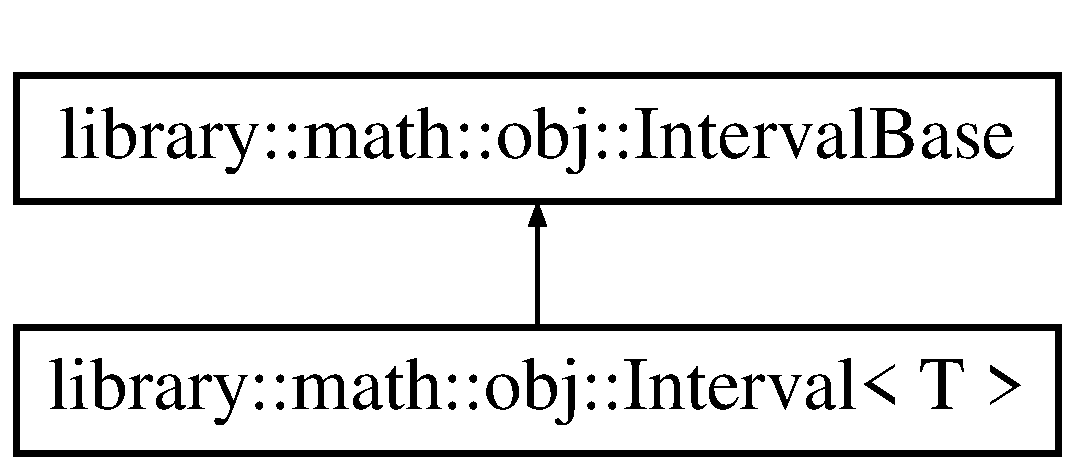
\includegraphics[height=2.000000cm]{classlibrary_1_1math_1_1obj_1_1_interval}
\end{center}
\end{figure}
\subsection*{Public Member Functions}
\begin{DoxyCompactItemize}
\item 
\hyperlink{classlibrary_1_1math_1_1obj_1_1_interval_ad3c3506ca4e90506ab1ea25a18fc5cd7}{Interval} (const T \&a\+Lower\+Bound, const T \&an\+Upper\+Bound, const \hyperlink{classlibrary_1_1math_1_1obj_1_1_interval_base_aabce6fa07a6e2e8fd3fcab5fd0d317d6}{Interval\+::\+Type} \&an\+Interval\+Type)
\begin{DoxyCompactList}\small\item\em Constructor. \end{DoxyCompactList}\item 
bool \hyperlink{classlibrary_1_1math_1_1obj_1_1_interval_a99b12768e33b75bf87ab656b92c03e98}{operator==} (const \hyperlink{classlibrary_1_1math_1_1obj_1_1_interval}{Interval} \&an\+Interval) const
\begin{DoxyCompactList}\small\item\em Equal to operator. \end{DoxyCompactList}\item 
bool \hyperlink{classlibrary_1_1math_1_1obj_1_1_interval_a5ca4c08ba0aff1ea42ea3804d51e02cf}{operator!=} (const \hyperlink{classlibrary_1_1math_1_1obj_1_1_interval}{Interval} \&an\+Interval) const
\begin{DoxyCompactList}\small\item\em Not equal to operator. \end{DoxyCompactList}\item 
bool \hyperlink{classlibrary_1_1math_1_1obj_1_1_interval_a2de37bb9d7b97ae7892188c26c99b6fb}{is\+Defined} () const
\begin{DoxyCompactList}\small\item\em Check if interval is defined. \end{DoxyCompactList}\item 
bool \hyperlink{classlibrary_1_1math_1_1obj_1_1_interval_a0e9997639f0c415f4f7fe8dcb58e13a8}{is\+Degenerate} () const
\begin{DoxyCompactList}\small\item\em Check if interval is degenerate, i.\+e. its lower and upper bounds are the equal. \end{DoxyCompactList}\item 
bool \hyperlink{classlibrary_1_1math_1_1obj_1_1_interval_aba618feb6e4b6d052999c2b8c8c0b06a}{intersects} (const \hyperlink{classlibrary_1_1math_1_1obj_1_1_interval}{Interval} \&an\+Interval) const
\begin{DoxyCompactList}\small\item\em Check if interval is intersecting with another interval. \end{DoxyCompactList}\item 
bool \hyperlink{classlibrary_1_1math_1_1obj_1_1_interval_af100f4b53dc3211efde2733c19e458c3}{contains} (const T \&a\+Value) const
\begin{DoxyCompactList}\small\item\em Check if interval contains value. \end{DoxyCompactList}\item 
bool \hyperlink{classlibrary_1_1math_1_1obj_1_1_interval_a3bace75e3cfb5f5c737e642c08572d25}{contains} (const \hyperlink{classlibrary_1_1math_1_1obj_1_1_interval}{Interval} \&an\+Interval) const
\begin{DoxyCompactList}\small\item\em Check if interval contains another interval. \end{DoxyCompactList}\item 
const T \& \hyperlink{classlibrary_1_1math_1_1obj_1_1_interval_ada0dc68134cfacd5a0e959b492cea534}{access\+Lower\+Bound} () const
\begin{DoxyCompactList}\small\item\em Get reference to lower bound. \end{DoxyCompactList}\item 
const T \& \hyperlink{classlibrary_1_1math_1_1obj_1_1_interval_a99692ee706ae6de7cd274ceae3644138}{access\+Upper\+Bound} () const
\begin{DoxyCompactList}\small\item\em Get reference to upper bound. \end{DoxyCompactList}\item 
\hyperlink{classlibrary_1_1math_1_1obj_1_1_interval_base_aabce6fa07a6e2e8fd3fcab5fd0d317d6}{Interval\+::\+Type} \hyperlink{classlibrary_1_1math_1_1obj_1_1_interval_a881ab7e17883b4f1553d7e8ba9cc7656}{get\+Type} () const
\begin{DoxyCompactList}\small\item\em Get interval type. \end{DoxyCompactList}\item 
T \hyperlink{classlibrary_1_1math_1_1obj_1_1_interval_a4e01721016dd02dddc93fb012ff7d5b3}{get\+Lower\+Bound} () const
\begin{DoxyCompactList}\small\item\em Get lower bound. \end{DoxyCompactList}\item 
T \hyperlink{classlibrary_1_1math_1_1obj_1_1_interval_a97d09e9c5e7f67b6ddf162af01a8066e}{get\+Upper\+Bound} () const
\begin{DoxyCompactList}\small\item\em Get upper bound. \end{DoxyCompactList}\item 
\hyperlink{classlibrary_1_1math_1_1obj_1_1_interval}{Interval}$<$ T $>$ \hyperlink{classlibrary_1_1math_1_1obj_1_1_interval_a2f23ca14d71c454417270218132423de}{get\+Intersection\+With} (const \hyperlink{classlibrary_1_1math_1_1obj_1_1_interval}{Interval} \&an\+Interval) const
\begin{DoxyCompactList}\small\item\em Get intersecting interval with another interval. \end{DoxyCompactList}\item 
\hyperlink{classlibrary_1_1math_1_1obj_1_1_interval}{Interval}$<$ T $>$ \hyperlink{classlibrary_1_1math_1_1obj_1_1_interval_a4183db388b6a63429a031d3687b20ecf}{get\+Union\+With} (const \hyperlink{classlibrary_1_1math_1_1obj_1_1_interval}{Interval} \&an\+Interval) const
\begin{DoxyCompactList}\small\item\em Get union interval with another interval. \end{DoxyCompactList}\item 
{\footnotesize template$<$class U $>$ }\\ctnr\+::\+Array$<$ T $>$ \hyperlink{classlibrary_1_1math_1_1obj_1_1_interval_ad453aeaec68c18421a7c93ac7c14fa48}{generate\+Array\+With\+Step} (const U \&a\+Step) const
\begin{DoxyCompactList}\small\item\em Generate array from a given step. \end{DoxyCompactList}\item 
ctnr\+::\+Array$<$ T $>$ \hyperlink{classlibrary_1_1math_1_1obj_1_1_interval_a250e05a1f463f107952b437e5ff4f4d2}{generate\+Array\+With\+Size} (const types\+::\+Size \&an\+Array\+Size) const
\begin{DoxyCompactList}\small\item\em Generate array with a given size. \end{DoxyCompactList}\item 
types\+::\+String \hyperlink{classlibrary_1_1math_1_1obj_1_1_interval_ad75c400daf533c35bc91da8c50b00a9e}{to\+String} () const
\begin{DoxyCompactList}\small\item\em Get serialized interval. \end{DoxyCompactList}\item 
void \hyperlink{classlibrary_1_1math_1_1obj_1_1_interval_a4dfb117d5a9c23bd32a3631fcf3686ec}{set\+Type} (const \hyperlink{classlibrary_1_1math_1_1obj_1_1_interval_base_aabce6fa07a6e2e8fd3fcab5fd0d317d6}{Interval\+::\+Type} \&a\+Type)
\begin{DoxyCompactList}\small\item\em \hyperlink{classlibrary_1_1math_1_1obj_1_1_interval}{Interval} type setter. \end{DoxyCompactList}\item 
void \hyperlink{classlibrary_1_1math_1_1obj_1_1_interval_a5ceb8fb56f920193c8b18346992b5d02}{set\+Lower\+Bound} (const T \&a\+Lower\+Bound)
\begin{DoxyCompactList}\small\item\em \hyperlink{classlibrary_1_1math_1_1obj_1_1_interval}{Interval} lower bound setter. \end{DoxyCompactList}\item 
void \hyperlink{classlibrary_1_1math_1_1obj_1_1_interval_a9c6b857d9fad97969635f669428c2b48}{set\+Upper\+Bound} (const T \&an\+Upper\+Bound)
\begin{DoxyCompactList}\small\item\em \hyperlink{classlibrary_1_1math_1_1obj_1_1_interval}{Interval} upper bound setter. \end{DoxyCompactList}\end{DoxyCompactItemize}
\subsection*{Static Public Member Functions}
\begin{DoxyCompactItemize}
\item 
static \hyperlink{classlibrary_1_1math_1_1obj_1_1_interval}{Interval}$<$ T $>$ \hyperlink{classlibrary_1_1math_1_1obj_1_1_interval_a415849a8c5306d6811612a842a5d0a40}{Undefined} ()
\begin{DoxyCompactList}\small\item\em Constructs an undefined interval. \end{DoxyCompactList}\item 
static \hyperlink{classlibrary_1_1math_1_1obj_1_1_interval}{Interval}$<$ T $>$ \hyperlink{classlibrary_1_1math_1_1obj_1_1_interval_aae8bb2b89af450729338d48563def4d7}{Closed} (const T \&a\+Lower\+Bound, const T \&an\+Upper\+Bound)
\begin{DoxyCompactList}\small\item\em Constructs a closed interval. \end{DoxyCompactList}\item 
static \hyperlink{classlibrary_1_1math_1_1obj_1_1_interval}{Interval}$<$ T $>$ \hyperlink{classlibrary_1_1math_1_1obj_1_1_interval_add0e1114a0c153da7a928fd059a08919}{Open} (const T \&a\+Lower\+Bound, const T \&an\+Upper\+Bound)
\begin{DoxyCompactList}\small\item\em Constructs an open interval. \end{DoxyCompactList}\item 
static \hyperlink{classlibrary_1_1math_1_1obj_1_1_interval}{Interval}$<$ T $>$ \hyperlink{classlibrary_1_1math_1_1obj_1_1_interval_a7e706c1e5133c731645e7633a9d763bd}{Half\+Open\+Left} (const T \&a\+Lower\+Bound, const T \&an\+Upper\+Bound)
\begin{DoxyCompactList}\small\item\em Constructs an half-\/open left interval. \end{DoxyCompactList}\item 
static \hyperlink{classlibrary_1_1math_1_1obj_1_1_interval}{Interval}$<$ T $>$ \hyperlink{classlibrary_1_1math_1_1obj_1_1_interval_a1a15d0518cc69fa3e442fc39c0622477}{Half\+Open\+Right} (const T \&a\+Lower\+Bound, const T \&an\+Upper\+Bound)
\begin{DoxyCompactList}\small\item\em Constructs an half-\/open right interval. \end{DoxyCompactList}\item 
static \hyperlink{classlibrary_1_1math_1_1obj_1_1_interval}{Interval}$<$ T $>$ \hyperlink{classlibrary_1_1math_1_1obj_1_1_interval_a9ed15c38ee04880a1aba75defa086a79}{Parse} (const types\+::\+String \&a\+String)
\begin{DoxyCompactList}\small\item\em Constructs an interval from a given string. \end{DoxyCompactList}\item 
static types\+::\+String \hyperlink{classlibrary_1_1math_1_1obj_1_1_interval_a64a1850152db9b95c9824c71378d9f40}{String\+From\+Type} (const \hyperlink{classlibrary_1_1math_1_1obj_1_1_interval_base_aabce6fa07a6e2e8fd3fcab5fd0d317d6}{Interval\+::\+Type} \&an\+Interval\+Type)
\begin{DoxyCompactList}\small\item\em Converts interval type to string. \end{DoxyCompactList}\end{DoxyCompactItemize}
\subsection*{Friends}
\begin{DoxyCompactItemize}
\item 
{\footnotesize template$<$class U $>$ }\\std\+::ostream \& \hyperlink{classlibrary_1_1math_1_1obj_1_1_interval_a3aa32afa8cb5d85eeb45540b0bf5657b}{operator$<$$<$} (std\+::ostream \&an\+Output\+Stream, const \hyperlink{classlibrary_1_1math_1_1obj_1_1_interval}{Interval}$<$ U $>$ \&an\+Interval)
\begin{DoxyCompactList}\small\item\em Output stream operator. \end{DoxyCompactList}\end{DoxyCompactItemize}
\subsection*{Additional Inherited Members}


\subsection{Detailed Description}
\subsubsection*{template$<$class T$>$\newline
class library\+::math\+::obj\+::\+Interval$<$ T $>$}

Set of numbers with the property that any number that lies between two numbers in the set is also included in the set. 

https\+://en.wikipedia.\+org/wiki/\+Interval\+\_\+(mathematics) 

\subsection{Constructor \& Destructor Documentation}
\mbox{\Hypertarget{classlibrary_1_1math_1_1obj_1_1_interval_ad3c3506ca4e90506ab1ea25a18fc5cd7}\label{classlibrary_1_1math_1_1obj_1_1_interval_ad3c3506ca4e90506ab1ea25a18fc5cd7}} 
\index{library\+::math\+::obj\+::\+Interval@{library\+::math\+::obj\+::\+Interval}!Interval@{Interval}}
\index{Interval@{Interval}!library\+::math\+::obj\+::\+Interval@{library\+::math\+::obj\+::\+Interval}}
\subsubsection{\texorpdfstring{Interval()}{Interval()}}
{\footnotesize\ttfamily template$<$class T$>$ \\
\hyperlink{classlibrary_1_1math_1_1obj_1_1_interval}{library\+::math\+::obj\+::\+Interval}$<$ T $>$\+::\hyperlink{classlibrary_1_1math_1_1obj_1_1_interval}{Interval} (\begin{DoxyParamCaption}\item[{const T \&}]{a\+Lower\+Bound,  }\item[{const T \&}]{an\+Upper\+Bound,  }\item[{const \hyperlink{classlibrary_1_1math_1_1obj_1_1_interval}{Interval}$<$ T $>$\+::\hyperlink{classlibrary_1_1math_1_1obj_1_1_interval_base_aabce6fa07a6e2e8fd3fcab5fd0d317d6}{Type} \&}]{an\+Interval\+Type }\end{DoxyParamCaption})}



Constructor. 


\begin{DoxyCode}
Interval<Real> interval(0.0, 1.0, \hyperlink{classlibrary_1_1math_1_1obj_1_1_interval_base_aabce6fa07a6e2e8fd3fcab5fd0d317d6a03f4a47830f97377a35321051685071e}{Interval::Type::Closed}) ;
\end{DoxyCode}



\begin{DoxyParams}[1]{Parameters}
\mbox{\tt in}  & {\em a\+Lower\+Bound} & A lower bound \\
\hline
\mbox{\tt in}  & {\em an\+Upper\+Bound} & An upper bound \\
\hline
\mbox{\tt in}  & {\em an\+Interval\+Type} & An interval type \\
\hline
\end{DoxyParams}


\subsection{Member Function Documentation}
\mbox{\Hypertarget{classlibrary_1_1math_1_1obj_1_1_interval_ada0dc68134cfacd5a0e959b492cea534}\label{classlibrary_1_1math_1_1obj_1_1_interval_ada0dc68134cfacd5a0e959b492cea534}} 
\index{library\+::math\+::obj\+::\+Interval@{library\+::math\+::obj\+::\+Interval}!access\+Lower\+Bound@{access\+Lower\+Bound}}
\index{access\+Lower\+Bound@{access\+Lower\+Bound}!library\+::math\+::obj\+::\+Interval@{library\+::math\+::obj\+::\+Interval}}
\subsubsection{\texorpdfstring{access\+Lower\+Bound()}{accessLowerBound()}}
{\footnotesize\ttfamily template$<$class T$>$ \\
const T\& \hyperlink{classlibrary_1_1math_1_1obj_1_1_interval}{library\+::math\+::obj\+::\+Interval}$<$ T $>$\+::access\+Lower\+Bound (\begin{DoxyParamCaption}{ }\end{DoxyParamCaption}) const}



Get reference to lower bound. 


\begin{DoxyCode}
Interval<Real> interval = \hyperlink{classlibrary_1_1math_1_1obj_1_1_interval_aae8bb2b89af450729338d48563def4d7}{Interval<Real>::Closed}(0.0, 1.0) ;
interval.accessLowerBound() ; \textcolor{comment}{// &0.0}
\end{DoxyCode}


\begin{DoxyReturn}{Returns}
Reference to lower bound 
\end{DoxyReturn}
\mbox{\Hypertarget{classlibrary_1_1math_1_1obj_1_1_interval_a99692ee706ae6de7cd274ceae3644138}\label{classlibrary_1_1math_1_1obj_1_1_interval_a99692ee706ae6de7cd274ceae3644138}} 
\index{library\+::math\+::obj\+::\+Interval@{library\+::math\+::obj\+::\+Interval}!access\+Upper\+Bound@{access\+Upper\+Bound}}
\index{access\+Upper\+Bound@{access\+Upper\+Bound}!library\+::math\+::obj\+::\+Interval@{library\+::math\+::obj\+::\+Interval}}
\subsubsection{\texorpdfstring{access\+Upper\+Bound()}{accessUpperBound()}}
{\footnotesize\ttfamily template$<$class T$>$ \\
const T\& \hyperlink{classlibrary_1_1math_1_1obj_1_1_interval}{library\+::math\+::obj\+::\+Interval}$<$ T $>$\+::access\+Upper\+Bound (\begin{DoxyParamCaption}{ }\end{DoxyParamCaption}) const}



Get reference to upper bound. 


\begin{DoxyCode}
Interval<Real> interval = \hyperlink{classlibrary_1_1math_1_1obj_1_1_interval_aae8bb2b89af450729338d48563def4d7}{Interval<Real>::Closed}(0.0, 1.0) ;
interval.accessUpperBound() ; \textcolor{comment}{// &1.0}
\end{DoxyCode}


\begin{DoxyReturn}{Returns}
Reference to upper bound 
\end{DoxyReturn}
\mbox{\Hypertarget{classlibrary_1_1math_1_1obj_1_1_interval_aae8bb2b89af450729338d48563def4d7}\label{classlibrary_1_1math_1_1obj_1_1_interval_aae8bb2b89af450729338d48563def4d7}} 
\index{library\+::math\+::obj\+::\+Interval@{library\+::math\+::obj\+::\+Interval}!Closed@{Closed}}
\index{Closed@{Closed}!library\+::math\+::obj\+::\+Interval@{library\+::math\+::obj\+::\+Interval}}
\subsubsection{\texorpdfstring{Closed()}{Closed()}}
{\footnotesize\ttfamily template$<$class T$>$ \\
static \hyperlink{classlibrary_1_1math_1_1obj_1_1_interval}{Interval}$<$T$>$ \hyperlink{classlibrary_1_1math_1_1obj_1_1_interval}{library\+::math\+::obj\+::\+Interval}$<$ T $>$\+::Closed (\begin{DoxyParamCaption}\item[{const T \&}]{a\+Lower\+Bound,  }\item[{const T \&}]{an\+Upper\+Bound }\end{DoxyParamCaption})\hspace{0.3cm}{\ttfamily [static]}}



Constructs a closed interval. 


\begin{DoxyCode}
Interval<Real> interval = \hyperlink{classlibrary_1_1math_1_1obj_1_1_interval_aae8bb2b89af450729338d48563def4d7}{Interval<Real>::Closed}(0.0, 1.0) ; \textcolor{comment}{// [0.0, 1.0]}
\end{DoxyCode}


\begin{DoxyReturn}{Returns}
Closed interval 
\end{DoxyReturn}
\mbox{\Hypertarget{classlibrary_1_1math_1_1obj_1_1_interval_af100f4b53dc3211efde2733c19e458c3}\label{classlibrary_1_1math_1_1obj_1_1_interval_af100f4b53dc3211efde2733c19e458c3}} 
\index{library\+::math\+::obj\+::\+Interval@{library\+::math\+::obj\+::\+Interval}!contains@{contains}}
\index{contains@{contains}!library\+::math\+::obj\+::\+Interval@{library\+::math\+::obj\+::\+Interval}}
\subsubsection{\texorpdfstring{contains()}{contains()}\hspace{0.1cm}{\footnotesize\ttfamily [1/2]}}
{\footnotesize\ttfamily template$<$class T$>$ \\
bool \hyperlink{classlibrary_1_1math_1_1obj_1_1_interval}{library\+::math\+::obj\+::\+Interval}$<$ T $>$\+::contains (\begin{DoxyParamCaption}\item[{const T \&}]{a\+Value }\end{DoxyParamCaption}) const}



Check if interval contains value. 


\begin{DoxyCode}
\hyperlink{classlibrary_1_1math_1_1obj_1_1_interval_aae8bb2b89af450729338d48563def4d7}{Interval<Real>::Closed}(0.0, 1.0).contains(0.5) ; \textcolor{comment}{// True}
\end{DoxyCode}



\begin{DoxyParams}[1]{Parameters}
\mbox{\tt in}  & {\em a\+Value} & A value \\
\hline
\end{DoxyParams}
\begin{DoxyReturn}{Returns}
True if interval contains value 
\end{DoxyReturn}
\mbox{\Hypertarget{classlibrary_1_1math_1_1obj_1_1_interval_a3bace75e3cfb5f5c737e642c08572d25}\label{classlibrary_1_1math_1_1obj_1_1_interval_a3bace75e3cfb5f5c737e642c08572d25}} 
\index{library\+::math\+::obj\+::\+Interval@{library\+::math\+::obj\+::\+Interval}!contains@{contains}}
\index{contains@{contains}!library\+::math\+::obj\+::\+Interval@{library\+::math\+::obj\+::\+Interval}}
\subsubsection{\texorpdfstring{contains()}{contains()}\hspace{0.1cm}{\footnotesize\ttfamily [2/2]}}
{\footnotesize\ttfamily template$<$class T$>$ \\
bool \hyperlink{classlibrary_1_1math_1_1obj_1_1_interval}{library\+::math\+::obj\+::\+Interval}$<$ T $>$\+::contains (\begin{DoxyParamCaption}\item[{const \hyperlink{classlibrary_1_1math_1_1obj_1_1_interval}{Interval}$<$ T $>$ \&}]{an\+Interval }\end{DoxyParamCaption}) const}



Check if interval contains another interval. 


\begin{DoxyCode}
\hyperlink{classlibrary_1_1math_1_1obj_1_1_interval_aae8bb2b89af450729338d48563def4d7}{Interval<Real>::Closed}(0.0, 1.0).contains(
      \hyperlink{classlibrary_1_1math_1_1obj_1_1_interval_add0e1114a0c153da7a928fd059a08919}{Interval<Real>::Open}(0.2, 0.8)) ; \textcolor{comment}{// True}
\end{DoxyCode}



\begin{DoxyParams}[1]{Parameters}
\mbox{\tt in}  & {\em an\+Interval} & An interval \\
\hline
\end{DoxyParams}
\begin{DoxyReturn}{Returns}
True if interval contains another interval 
\end{DoxyReturn}
\mbox{\Hypertarget{classlibrary_1_1math_1_1obj_1_1_interval_a250e05a1f463f107952b437e5ff4f4d2}\label{classlibrary_1_1math_1_1obj_1_1_interval_a250e05a1f463f107952b437e5ff4f4d2}} 
\index{library\+::math\+::obj\+::\+Interval@{library\+::math\+::obj\+::\+Interval}!generate\+Array\+With\+Size@{generate\+Array\+With\+Size}}
\index{generate\+Array\+With\+Size@{generate\+Array\+With\+Size}!library\+::math\+::obj\+::\+Interval@{library\+::math\+::obj\+::\+Interval}}
\subsubsection{\texorpdfstring{generate\+Array\+With\+Size()}{generateArrayWithSize()}}
{\footnotesize\ttfamily template$<$class T$>$ \\
ctnr\+::\+Array$<$T$>$ \hyperlink{classlibrary_1_1math_1_1obj_1_1_interval}{library\+::math\+::obj\+::\+Interval}$<$ T $>$\+::generate\+Array\+With\+Size (\begin{DoxyParamCaption}\item[{const types\+::\+Size \&}]{an\+Array\+Size }\end{DoxyParamCaption}) const}



Generate array with a given size. 


\begin{DoxyCode}
Interval<Real> interval = \hyperlink{classlibrary_1_1math_1_1obj_1_1_interval_aae8bb2b89af450729338d48563def4d7}{Interval<Real>::Closed}(0.0, 1.0) ;
Array<Real> array = interval.generateArrayWithSize(3) ; \textcolor{comment}{// [0.0, 0.5, 1.0]}
\end{DoxyCode}



\begin{DoxyParams}[1]{Parameters}
\mbox{\tt in}  & {\em an\+Array\+Size} & An array size \\
\hline
\end{DoxyParams}
\begin{DoxyReturn}{Returns}
Array of values 
\end{DoxyReturn}
\mbox{\Hypertarget{classlibrary_1_1math_1_1obj_1_1_interval_ad453aeaec68c18421a7c93ac7c14fa48}\label{classlibrary_1_1math_1_1obj_1_1_interval_ad453aeaec68c18421a7c93ac7c14fa48}} 
\index{library\+::math\+::obj\+::\+Interval@{library\+::math\+::obj\+::\+Interval}!generate\+Array\+With\+Step@{generate\+Array\+With\+Step}}
\index{generate\+Array\+With\+Step@{generate\+Array\+With\+Step}!library\+::math\+::obj\+::\+Interval@{library\+::math\+::obj\+::\+Interval}}
\subsubsection{\texorpdfstring{generate\+Array\+With\+Step()}{generateArrayWithStep()}}
{\footnotesize\ttfamily template$<$class T$>$ \\
template$<$class U $>$ \\
ctnr\+::\+Array$<$T$>$ \hyperlink{classlibrary_1_1math_1_1obj_1_1_interval}{library\+::math\+::obj\+::\+Interval}$<$ T $>$\+::generate\+Array\+With\+Step (\begin{DoxyParamCaption}\item[{const U \&}]{a\+Step }\end{DoxyParamCaption}) const}



Generate array from a given step. 


\begin{DoxyCode}
Interval<Real> interval = \hyperlink{classlibrary_1_1math_1_1obj_1_1_interval_aae8bb2b89af450729338d48563def4d7}{Interval<Real>::Closed}(0.0, 1.0) ;
Array<Real> array = interval.generateArrayWithStep(0.5) ; \textcolor{comment}{// [0.0, 0.5, 1.0]}
\end{DoxyCode}



\begin{DoxyParams}[1]{Parameters}
\mbox{\tt in}  & {\em a\+Step} & A step \\
\hline
\end{DoxyParams}
\begin{DoxyReturn}{Returns}
Array of values 
\end{DoxyReturn}
\mbox{\Hypertarget{classlibrary_1_1math_1_1obj_1_1_interval_a2f23ca14d71c454417270218132423de}\label{classlibrary_1_1math_1_1obj_1_1_interval_a2f23ca14d71c454417270218132423de}} 
\index{library\+::math\+::obj\+::\+Interval@{library\+::math\+::obj\+::\+Interval}!get\+Intersection\+With@{get\+Intersection\+With}}
\index{get\+Intersection\+With@{get\+Intersection\+With}!library\+::math\+::obj\+::\+Interval@{library\+::math\+::obj\+::\+Interval}}
\subsubsection{\texorpdfstring{get\+Intersection\+With()}{getIntersectionWith()}}
{\footnotesize\ttfamily template$<$class T$>$ \\
\hyperlink{classlibrary_1_1math_1_1obj_1_1_interval}{Interval}$<$T$>$ \hyperlink{classlibrary_1_1math_1_1obj_1_1_interval}{library\+::math\+::obj\+::\+Interval}$<$ T $>$\+::get\+Intersection\+With (\begin{DoxyParamCaption}\item[{const \hyperlink{classlibrary_1_1math_1_1obj_1_1_interval}{Interval}$<$ T $>$ \&}]{an\+Interval }\end{DoxyParamCaption}) const}



Get intersecting interval with another interval. 


\begin{DoxyCode}
Interval<Real> firstInterval = \hyperlink{classlibrary_1_1math_1_1obj_1_1_interval_aae8bb2b89af450729338d48563def4d7}{Interval<Real>::Closed}(0.0, 1.0) ;
Interval<Real> secondInterval = \hyperlink{classlibrary_1_1math_1_1obj_1_1_interval_aae8bb2b89af450729338d48563def4d7}{Interval<Real>::Closed}(0.5, 1.5) ;
Interval<Real> intersection = firstInterval.getIntersectionWith(secondInterval) ; \textcolor{comment}{// [0.5, 1.0]}
\end{DoxyCode}



\begin{DoxyParams}[1]{Parameters}
\mbox{\tt in}  & {\em an\+Interval} & An interval \\
\hline
\end{DoxyParams}
\begin{DoxyReturn}{Returns}
Intersecting interval 
\end{DoxyReturn}
\mbox{\Hypertarget{classlibrary_1_1math_1_1obj_1_1_interval_a4e01721016dd02dddc93fb012ff7d5b3}\label{classlibrary_1_1math_1_1obj_1_1_interval_a4e01721016dd02dddc93fb012ff7d5b3}} 
\index{library\+::math\+::obj\+::\+Interval@{library\+::math\+::obj\+::\+Interval}!get\+Lower\+Bound@{get\+Lower\+Bound}}
\index{get\+Lower\+Bound@{get\+Lower\+Bound}!library\+::math\+::obj\+::\+Interval@{library\+::math\+::obj\+::\+Interval}}
\subsubsection{\texorpdfstring{get\+Lower\+Bound()}{getLowerBound()}}
{\footnotesize\ttfamily template$<$class T$>$ \\
T \hyperlink{classlibrary_1_1math_1_1obj_1_1_interval}{library\+::math\+::obj\+::\+Interval}$<$ T $>$\+::get\+Lower\+Bound (\begin{DoxyParamCaption}{ }\end{DoxyParamCaption}) const}



Get lower bound. 


\begin{DoxyCode}
Interval<Real> interval = \hyperlink{classlibrary_1_1math_1_1obj_1_1_interval_aae8bb2b89af450729338d48563def4d7}{Interval<Real>::Closed}(0.0, 1.0) ;
interval.getLowerBound() ; \textcolor{comment}{// 0.0}
\end{DoxyCode}


\begin{DoxyReturn}{Returns}
Lower bound 
\end{DoxyReturn}
\mbox{\Hypertarget{classlibrary_1_1math_1_1obj_1_1_interval_a881ab7e17883b4f1553d7e8ba9cc7656}\label{classlibrary_1_1math_1_1obj_1_1_interval_a881ab7e17883b4f1553d7e8ba9cc7656}} 
\index{library\+::math\+::obj\+::\+Interval@{library\+::math\+::obj\+::\+Interval}!get\+Type@{get\+Type}}
\index{get\+Type@{get\+Type}!library\+::math\+::obj\+::\+Interval@{library\+::math\+::obj\+::\+Interval}}
\subsubsection{\texorpdfstring{get\+Type()}{getType()}}
{\footnotesize\ttfamily template$<$class T$>$ \\
\hyperlink{classlibrary_1_1math_1_1obj_1_1_interval_base_aabce6fa07a6e2e8fd3fcab5fd0d317d6}{Interval\+::\+Type} \hyperlink{classlibrary_1_1math_1_1obj_1_1_interval}{library\+::math\+::obj\+::\+Interval}$<$ T $>$\+::get\+Type (\begin{DoxyParamCaption}{ }\end{DoxyParamCaption}) const}



Get interval type. 


\begin{DoxyCode}
Interval<Real> interval = \hyperlink{classlibrary_1_1math_1_1obj_1_1_interval_aae8bb2b89af450729338d48563def4d7}{Interval<Real>::Closed}(0.0, 1.0) ;
interval.getType() ; \textcolor{comment}{// Interval<Real>::Type::Closed}
\end{DoxyCode}


\begin{DoxyReturn}{Returns}
\hyperlink{classlibrary_1_1math_1_1obj_1_1_interval}{Interval} type 
\end{DoxyReturn}
\mbox{\Hypertarget{classlibrary_1_1math_1_1obj_1_1_interval_a4183db388b6a63429a031d3687b20ecf}\label{classlibrary_1_1math_1_1obj_1_1_interval_a4183db388b6a63429a031d3687b20ecf}} 
\index{library\+::math\+::obj\+::\+Interval@{library\+::math\+::obj\+::\+Interval}!get\+Union\+With@{get\+Union\+With}}
\index{get\+Union\+With@{get\+Union\+With}!library\+::math\+::obj\+::\+Interval@{library\+::math\+::obj\+::\+Interval}}
\subsubsection{\texorpdfstring{get\+Union\+With()}{getUnionWith()}}
{\footnotesize\ttfamily template$<$class T$>$ \\
\hyperlink{classlibrary_1_1math_1_1obj_1_1_interval}{Interval}$<$T$>$ \hyperlink{classlibrary_1_1math_1_1obj_1_1_interval}{library\+::math\+::obj\+::\+Interval}$<$ T $>$\+::get\+Union\+With (\begin{DoxyParamCaption}\item[{const \hyperlink{classlibrary_1_1math_1_1obj_1_1_interval}{Interval}$<$ T $>$ \&}]{an\+Interval }\end{DoxyParamCaption}) const}



Get union interval with another interval. 


\begin{DoxyCode}
Interval<Real> firstInterval = \hyperlink{classlibrary_1_1math_1_1obj_1_1_interval_aae8bb2b89af450729338d48563def4d7}{Interval<Real>::Closed}(0.0, 1.0) ;
Interval<Real> secondInterval = \hyperlink{classlibrary_1_1math_1_1obj_1_1_interval_aae8bb2b89af450729338d48563def4d7}{Interval<Real>::Closed}(0.5, 1.5) ;
Interval<Real> \textcolor{keyword}{union }= firstInterval.\hyperlink{classlibrary_1_1math_1_1obj_1_1_interval_a4183db388b6a63429a031d3687b20ecf}{getUnionWith}(secondInterval) ; \textcolor{comment}{// [0.0, 1.5]}
\end{DoxyCode}



\begin{DoxyParams}[1]{Parameters}
\mbox{\tt in}  & {\em an\+Interval} & An interval \\
\hline
\end{DoxyParams}
\begin{DoxyReturn}{Returns}
Union interval 
\end{DoxyReturn}
\mbox{\Hypertarget{classlibrary_1_1math_1_1obj_1_1_interval_a97d09e9c5e7f67b6ddf162af01a8066e}\label{classlibrary_1_1math_1_1obj_1_1_interval_a97d09e9c5e7f67b6ddf162af01a8066e}} 
\index{library\+::math\+::obj\+::\+Interval@{library\+::math\+::obj\+::\+Interval}!get\+Upper\+Bound@{get\+Upper\+Bound}}
\index{get\+Upper\+Bound@{get\+Upper\+Bound}!library\+::math\+::obj\+::\+Interval@{library\+::math\+::obj\+::\+Interval}}
\subsubsection{\texorpdfstring{get\+Upper\+Bound()}{getUpperBound()}}
{\footnotesize\ttfamily template$<$class T$>$ \\
T \hyperlink{classlibrary_1_1math_1_1obj_1_1_interval}{library\+::math\+::obj\+::\+Interval}$<$ T $>$\+::get\+Upper\+Bound (\begin{DoxyParamCaption}{ }\end{DoxyParamCaption}) const}



Get upper bound. 


\begin{DoxyCode}
Interval<Real> interval = \hyperlink{classlibrary_1_1math_1_1obj_1_1_interval_aae8bb2b89af450729338d48563def4d7}{Interval<Real>::Closed}(0.0, 1.0) ;
interval.getUpperBound() ; \textcolor{comment}{// 1.0}
\end{DoxyCode}


\begin{DoxyReturn}{Returns}
Upper bound 
\end{DoxyReturn}
\mbox{\Hypertarget{classlibrary_1_1math_1_1obj_1_1_interval_a7e706c1e5133c731645e7633a9d763bd}\label{classlibrary_1_1math_1_1obj_1_1_interval_a7e706c1e5133c731645e7633a9d763bd}} 
\index{library\+::math\+::obj\+::\+Interval@{library\+::math\+::obj\+::\+Interval}!Half\+Open\+Left@{Half\+Open\+Left}}
\index{Half\+Open\+Left@{Half\+Open\+Left}!library\+::math\+::obj\+::\+Interval@{library\+::math\+::obj\+::\+Interval}}
\subsubsection{\texorpdfstring{Half\+Open\+Left()}{HalfOpenLeft()}}
{\footnotesize\ttfamily template$<$class T$>$ \\
static \hyperlink{classlibrary_1_1math_1_1obj_1_1_interval}{Interval}$<$T$>$ \hyperlink{classlibrary_1_1math_1_1obj_1_1_interval}{library\+::math\+::obj\+::\+Interval}$<$ T $>$\+::Half\+Open\+Left (\begin{DoxyParamCaption}\item[{const T \&}]{a\+Lower\+Bound,  }\item[{const T \&}]{an\+Upper\+Bound }\end{DoxyParamCaption})\hspace{0.3cm}{\ttfamily [static]}}



Constructs an half-\/open left interval. 


\begin{DoxyCode}
Interval<Real> interval = \hyperlink{classlibrary_1_1math_1_1obj_1_1_interval_a7e706c1e5133c731645e7633a9d763bd}{Interval<Real>::HalfOpenLeft}(0.0, 1.0) ; \textcolor{comment}{// ]0.0,
       1.0]}
\end{DoxyCode}


\begin{DoxyReturn}{Returns}
Half-\/open left interval 
\end{DoxyReturn}
\mbox{\Hypertarget{classlibrary_1_1math_1_1obj_1_1_interval_a1a15d0518cc69fa3e442fc39c0622477}\label{classlibrary_1_1math_1_1obj_1_1_interval_a1a15d0518cc69fa3e442fc39c0622477}} 
\index{library\+::math\+::obj\+::\+Interval@{library\+::math\+::obj\+::\+Interval}!Half\+Open\+Right@{Half\+Open\+Right}}
\index{Half\+Open\+Right@{Half\+Open\+Right}!library\+::math\+::obj\+::\+Interval@{library\+::math\+::obj\+::\+Interval}}
\subsubsection{\texorpdfstring{Half\+Open\+Right()}{HalfOpenRight()}}
{\footnotesize\ttfamily template$<$class T$>$ \\
static \hyperlink{classlibrary_1_1math_1_1obj_1_1_interval}{Interval}$<$T$>$ \hyperlink{classlibrary_1_1math_1_1obj_1_1_interval}{library\+::math\+::obj\+::\+Interval}$<$ T $>$\+::Half\+Open\+Right (\begin{DoxyParamCaption}\item[{const T \&}]{a\+Lower\+Bound,  }\item[{const T \&}]{an\+Upper\+Bound }\end{DoxyParamCaption})\hspace{0.3cm}{\ttfamily [static]}}



Constructs an half-\/open right interval. 


\begin{DoxyCode}
Interval<Real> interval = \hyperlink{classlibrary_1_1math_1_1obj_1_1_interval_a1a15d0518cc69fa3e442fc39c0622477}{Interval<Real>::HalfOpenRight}(0.0, 1.0) ; \textcolor{comment}{// [0.0,
       1.0[}
\end{DoxyCode}


\begin{DoxyReturn}{Returns}
Half-\/open right interval 
\end{DoxyReturn}
\mbox{\Hypertarget{classlibrary_1_1math_1_1obj_1_1_interval_aba618feb6e4b6d052999c2b8c8c0b06a}\label{classlibrary_1_1math_1_1obj_1_1_interval_aba618feb6e4b6d052999c2b8c8c0b06a}} 
\index{library\+::math\+::obj\+::\+Interval@{library\+::math\+::obj\+::\+Interval}!intersects@{intersects}}
\index{intersects@{intersects}!library\+::math\+::obj\+::\+Interval@{library\+::math\+::obj\+::\+Interval}}
\subsubsection{\texorpdfstring{intersects()}{intersects()}}
{\footnotesize\ttfamily template$<$class T$>$ \\
bool \hyperlink{classlibrary_1_1math_1_1obj_1_1_interval}{library\+::math\+::obj\+::\+Interval}$<$ T $>$\+::intersects (\begin{DoxyParamCaption}\item[{const \hyperlink{classlibrary_1_1math_1_1obj_1_1_interval}{Interval}$<$ T $>$ \&}]{an\+Interval }\end{DoxyParamCaption}) const}



Check if interval is intersecting with another interval. 


\begin{DoxyCode}
\hyperlink{classlibrary_1_1math_1_1obj_1_1_interval_aae8bb2b89af450729338d48563def4d7}{Interval<Real>::Closed}(0.0, 1.0).intersects(
      \hyperlink{classlibrary_1_1math_1_1obj_1_1_interval_aae8bb2b89af450729338d48563def4d7}{Interval<Real>::Closed}(0.5, 1.5)) ; \textcolor{comment}{// True}
\end{DoxyCode}



\begin{DoxyParams}[1]{Parameters}
\mbox{\tt in}  & {\em an\+Interval} & An interval \\
\hline
\end{DoxyParams}
\begin{DoxyReturn}{Returns}
True if intervals are intersecting 
\end{DoxyReturn}
\mbox{\Hypertarget{classlibrary_1_1math_1_1obj_1_1_interval_a2de37bb9d7b97ae7892188c26c99b6fb}\label{classlibrary_1_1math_1_1obj_1_1_interval_a2de37bb9d7b97ae7892188c26c99b6fb}} 
\index{library\+::math\+::obj\+::\+Interval@{library\+::math\+::obj\+::\+Interval}!is\+Defined@{is\+Defined}}
\index{is\+Defined@{is\+Defined}!library\+::math\+::obj\+::\+Interval@{library\+::math\+::obj\+::\+Interval}}
\subsubsection{\texorpdfstring{is\+Defined()}{isDefined()}}
{\footnotesize\ttfamily template$<$class T$>$ \\
bool \hyperlink{classlibrary_1_1math_1_1obj_1_1_interval}{library\+::math\+::obj\+::\+Interval}$<$ T $>$\+::is\+Defined (\begin{DoxyParamCaption}{ }\end{DoxyParamCaption}) const}



Check if interval is defined. 


\begin{DoxyCode}
\hyperlink{classlibrary_1_1math_1_1obj_1_1_interval_aae8bb2b89af450729338d48563def4d7}{Interval<Real>::Closed}(0.0, 1.0).isDefined() ; \textcolor{comment}{// True}
\end{DoxyCode}


\begin{DoxyReturn}{Returns}
True if interval is defined 
\end{DoxyReturn}
\mbox{\Hypertarget{classlibrary_1_1math_1_1obj_1_1_interval_a0e9997639f0c415f4f7fe8dcb58e13a8}\label{classlibrary_1_1math_1_1obj_1_1_interval_a0e9997639f0c415f4f7fe8dcb58e13a8}} 
\index{library\+::math\+::obj\+::\+Interval@{library\+::math\+::obj\+::\+Interval}!is\+Degenerate@{is\+Degenerate}}
\index{is\+Degenerate@{is\+Degenerate}!library\+::math\+::obj\+::\+Interval@{library\+::math\+::obj\+::\+Interval}}
\subsubsection{\texorpdfstring{is\+Degenerate()}{isDegenerate()}}
{\footnotesize\ttfamily template$<$class T$>$ \\
bool \hyperlink{classlibrary_1_1math_1_1obj_1_1_interval}{library\+::math\+::obj\+::\+Interval}$<$ T $>$\+::is\+Degenerate (\begin{DoxyParamCaption}{ }\end{DoxyParamCaption}) const}



Check if interval is degenerate, i.\+e. its lower and upper bounds are the equal. 


\begin{DoxyCode}
\hyperlink{classlibrary_1_1math_1_1obj_1_1_interval_aae8bb2b89af450729338d48563def4d7}{Interval<Real>::Closed}(1.0, 1.0).isDegenerate() ; \textcolor{comment}{// True}
\end{DoxyCode}


\begin{DoxyReturn}{Returns}
True if interval is degenerate 
\end{DoxyReturn}
\mbox{\Hypertarget{classlibrary_1_1math_1_1obj_1_1_interval_add0e1114a0c153da7a928fd059a08919}\label{classlibrary_1_1math_1_1obj_1_1_interval_add0e1114a0c153da7a928fd059a08919}} 
\index{library\+::math\+::obj\+::\+Interval@{library\+::math\+::obj\+::\+Interval}!Open@{Open}}
\index{Open@{Open}!library\+::math\+::obj\+::\+Interval@{library\+::math\+::obj\+::\+Interval}}
\subsubsection{\texorpdfstring{Open()}{Open()}}
{\footnotesize\ttfamily template$<$class T$>$ \\
static \hyperlink{classlibrary_1_1math_1_1obj_1_1_interval}{Interval}$<$T$>$ \hyperlink{classlibrary_1_1math_1_1obj_1_1_interval}{library\+::math\+::obj\+::\+Interval}$<$ T $>$\+::Open (\begin{DoxyParamCaption}\item[{const T \&}]{a\+Lower\+Bound,  }\item[{const T \&}]{an\+Upper\+Bound }\end{DoxyParamCaption})\hspace{0.3cm}{\ttfamily [static]}}



Constructs an open interval. 


\begin{DoxyCode}
Interval<Real> interval = \hyperlink{classlibrary_1_1math_1_1obj_1_1_interval_add0e1114a0c153da7a928fd059a08919}{Interval<Real>::Open}(0.0, 1.0) ; \textcolor{comment}{// ]0.0, 1.0[}
\end{DoxyCode}


\begin{DoxyReturn}{Returns}
Open interval 
\end{DoxyReturn}
\mbox{\Hypertarget{classlibrary_1_1math_1_1obj_1_1_interval_a5ca4c08ba0aff1ea42ea3804d51e02cf}\label{classlibrary_1_1math_1_1obj_1_1_interval_a5ca4c08ba0aff1ea42ea3804d51e02cf}} 
\index{library\+::math\+::obj\+::\+Interval@{library\+::math\+::obj\+::\+Interval}!operator"!=@{operator"!=}}
\index{operator"!=@{operator"!=}!library\+::math\+::obj\+::\+Interval@{library\+::math\+::obj\+::\+Interval}}
\subsubsection{\texorpdfstring{operator"!=()}{operator!=()}}
{\footnotesize\ttfamily template$<$class T$>$ \\
bool \hyperlink{classlibrary_1_1math_1_1obj_1_1_interval}{library\+::math\+::obj\+::\+Interval}$<$ T $>$\+::operator!= (\begin{DoxyParamCaption}\item[{const \hyperlink{classlibrary_1_1math_1_1obj_1_1_interval}{Interval}$<$ T $>$ \&}]{an\+Interval }\end{DoxyParamCaption}) const}



Not equal to operator. 


\begin{DoxyCode}
\hyperlink{classlibrary_1_1math_1_1obj_1_1_interval_aae8bb2b89af450729338d48563def4d7}{Interval<Real>::Closed}(0.0, 1.0) != \hyperlink{classlibrary_1_1math_1_1obj_1_1_interval_add0e1114a0c153da7a928fd059a08919}{Interval<Real>::Open}(0.0, 1.0
      ) ; \textcolor{comment}{// True}
\end{DoxyCode}



\begin{DoxyParams}[1]{Parameters}
\mbox{\tt in}  & {\em an\+Interval} & An interval \\
\hline
\end{DoxyParams}
\begin{DoxyReturn}{Returns}
True if intervals are not equal 
\end{DoxyReturn}
\mbox{\Hypertarget{classlibrary_1_1math_1_1obj_1_1_interval_a99b12768e33b75bf87ab656b92c03e98}\label{classlibrary_1_1math_1_1obj_1_1_interval_a99b12768e33b75bf87ab656b92c03e98}} 
\index{library\+::math\+::obj\+::\+Interval@{library\+::math\+::obj\+::\+Interval}!operator==@{operator==}}
\index{operator==@{operator==}!library\+::math\+::obj\+::\+Interval@{library\+::math\+::obj\+::\+Interval}}
\subsubsection{\texorpdfstring{operator==()}{operator==()}}
{\footnotesize\ttfamily template$<$class T$>$ \\
bool \hyperlink{classlibrary_1_1math_1_1obj_1_1_interval}{library\+::math\+::obj\+::\+Interval}$<$ T $>$\+::operator== (\begin{DoxyParamCaption}\item[{const \hyperlink{classlibrary_1_1math_1_1obj_1_1_interval}{Interval}$<$ T $>$ \&}]{an\+Interval }\end{DoxyParamCaption}) const}



Equal to operator. 


\begin{DoxyCode}
\hyperlink{classlibrary_1_1math_1_1obj_1_1_interval_aae8bb2b89af450729338d48563def4d7}{Interval<Real>::Closed}(0.0, 1.0) == \hyperlink{classlibrary_1_1math_1_1obj_1_1_interval_aae8bb2b89af450729338d48563def4d7}{Interval<Real>::Closed}(0.0,
       1.0) ; \textcolor{comment}{// True}
\end{DoxyCode}



\begin{DoxyParams}[1]{Parameters}
\mbox{\tt in}  & {\em an\+Interval} & An interval \\
\hline
\end{DoxyParams}
\begin{DoxyReturn}{Returns}
True if intervals are equal 
\end{DoxyReturn}
\mbox{\Hypertarget{classlibrary_1_1math_1_1obj_1_1_interval_a9ed15c38ee04880a1aba75defa086a79}\label{classlibrary_1_1math_1_1obj_1_1_interval_a9ed15c38ee04880a1aba75defa086a79}} 
\index{library\+::math\+::obj\+::\+Interval@{library\+::math\+::obj\+::\+Interval}!Parse@{Parse}}
\index{Parse@{Parse}!library\+::math\+::obj\+::\+Interval@{library\+::math\+::obj\+::\+Interval}}
\subsubsection{\texorpdfstring{Parse()}{Parse()}}
{\footnotesize\ttfamily template$<$class T$>$ \\
static \hyperlink{classlibrary_1_1math_1_1obj_1_1_interval}{Interval}$<$T$>$ \hyperlink{classlibrary_1_1math_1_1obj_1_1_interval}{library\+::math\+::obj\+::\+Interval}$<$ T $>$\+::Parse (\begin{DoxyParamCaption}\item[{const types\+::\+String \&}]{a\+String }\end{DoxyParamCaption})\hspace{0.3cm}{\ttfamily [static]}}



Constructs an interval from a given string. 


\begin{DoxyCode}
Interval<Real> interval = \hyperlink{classlibrary_1_1math_1_1obj_1_1_interval_a9ed15c38ee04880a1aba75defa086a79}{Interval<Real>::Parse}(\textcolor{stringliteral}{"[0.0, 1.0]"}) ; \textcolor{comment}{// [0.0, 1.0]}
\end{DoxyCode}



\begin{DoxyParams}[1]{Parameters}
\mbox{\tt in}  & {\em a\+String} & A string \\
\hline
\end{DoxyParams}
\begin{DoxyReturn}{Returns}
\hyperlink{classlibrary_1_1math_1_1obj_1_1_interval}{Interval} 
\end{DoxyReturn}
\mbox{\Hypertarget{classlibrary_1_1math_1_1obj_1_1_interval_a5ceb8fb56f920193c8b18346992b5d02}\label{classlibrary_1_1math_1_1obj_1_1_interval_a5ceb8fb56f920193c8b18346992b5d02}} 
\index{library\+::math\+::obj\+::\+Interval@{library\+::math\+::obj\+::\+Interval}!set\+Lower\+Bound@{set\+Lower\+Bound}}
\index{set\+Lower\+Bound@{set\+Lower\+Bound}!library\+::math\+::obj\+::\+Interval@{library\+::math\+::obj\+::\+Interval}}
\subsubsection{\texorpdfstring{set\+Lower\+Bound()}{setLowerBound()}}
{\footnotesize\ttfamily template$<$class T$>$ \\
void \hyperlink{classlibrary_1_1math_1_1obj_1_1_interval}{library\+::math\+::obj\+::\+Interval}$<$ T $>$\+::set\+Lower\+Bound (\begin{DoxyParamCaption}\item[{const T \&}]{a\+Lower\+Bound }\end{DoxyParamCaption})}



\hyperlink{classlibrary_1_1math_1_1obj_1_1_interval}{Interval} lower bound setter. 


\begin{DoxyParams}[1]{Parameters}
\mbox{\tt in}  & {\em a\+Lower\+Bound} & A lower bound \\
\hline
\end{DoxyParams}
\mbox{\Hypertarget{classlibrary_1_1math_1_1obj_1_1_interval_a4dfb117d5a9c23bd32a3631fcf3686ec}\label{classlibrary_1_1math_1_1obj_1_1_interval_a4dfb117d5a9c23bd32a3631fcf3686ec}} 
\index{library\+::math\+::obj\+::\+Interval@{library\+::math\+::obj\+::\+Interval}!set\+Type@{set\+Type}}
\index{set\+Type@{set\+Type}!library\+::math\+::obj\+::\+Interval@{library\+::math\+::obj\+::\+Interval}}
\subsubsection{\texorpdfstring{set\+Type()}{setType()}}
{\footnotesize\ttfamily template$<$class T$>$ \\
void \hyperlink{classlibrary_1_1math_1_1obj_1_1_interval}{library\+::math\+::obj\+::\+Interval}$<$ T $>$\+::set\+Type (\begin{DoxyParamCaption}\item[{const \hyperlink{classlibrary_1_1math_1_1obj_1_1_interval}{Interval}$<$ T $>$\+::\hyperlink{classlibrary_1_1math_1_1obj_1_1_interval_base_aabce6fa07a6e2e8fd3fcab5fd0d317d6}{Type} \&}]{a\+Type }\end{DoxyParamCaption})}



\hyperlink{classlibrary_1_1math_1_1obj_1_1_interval}{Interval} type setter. 


\begin{DoxyParams}[1]{Parameters}
\mbox{\tt in}  & {\em a\+Type} & An interval type \\
\hline
\end{DoxyParams}
\mbox{\Hypertarget{classlibrary_1_1math_1_1obj_1_1_interval_a9c6b857d9fad97969635f669428c2b48}\label{classlibrary_1_1math_1_1obj_1_1_interval_a9c6b857d9fad97969635f669428c2b48}} 
\index{library\+::math\+::obj\+::\+Interval@{library\+::math\+::obj\+::\+Interval}!set\+Upper\+Bound@{set\+Upper\+Bound}}
\index{set\+Upper\+Bound@{set\+Upper\+Bound}!library\+::math\+::obj\+::\+Interval@{library\+::math\+::obj\+::\+Interval}}
\subsubsection{\texorpdfstring{set\+Upper\+Bound()}{setUpperBound()}}
{\footnotesize\ttfamily template$<$class T$>$ \\
void \hyperlink{classlibrary_1_1math_1_1obj_1_1_interval}{library\+::math\+::obj\+::\+Interval}$<$ T $>$\+::set\+Upper\+Bound (\begin{DoxyParamCaption}\item[{const T \&}]{an\+Upper\+Bound }\end{DoxyParamCaption})}



\hyperlink{classlibrary_1_1math_1_1obj_1_1_interval}{Interval} upper bound setter. 


\begin{DoxyParams}[1]{Parameters}
\mbox{\tt in}  & {\em an\+Upper\+Bound} & An upper bound \\
\hline
\end{DoxyParams}
\mbox{\Hypertarget{classlibrary_1_1math_1_1obj_1_1_interval_a64a1850152db9b95c9824c71378d9f40}\label{classlibrary_1_1math_1_1obj_1_1_interval_a64a1850152db9b95c9824c71378d9f40}} 
\index{library\+::math\+::obj\+::\+Interval@{library\+::math\+::obj\+::\+Interval}!String\+From\+Type@{String\+From\+Type}}
\index{String\+From\+Type@{String\+From\+Type}!library\+::math\+::obj\+::\+Interval@{library\+::math\+::obj\+::\+Interval}}
\subsubsection{\texorpdfstring{String\+From\+Type()}{StringFromType()}}
{\footnotesize\ttfamily template$<$class T$>$ \\
static types\+::\+String \hyperlink{classlibrary_1_1math_1_1obj_1_1_interval}{library\+::math\+::obj\+::\+Interval}$<$ T $>$\+::String\+From\+Type (\begin{DoxyParamCaption}\item[{const \hyperlink{classlibrary_1_1math_1_1obj_1_1_interval}{Interval}$<$ T $>$\+::\hyperlink{classlibrary_1_1math_1_1obj_1_1_interval_base_aabce6fa07a6e2e8fd3fcab5fd0d317d6}{Type} \&}]{an\+Interval\+Type }\end{DoxyParamCaption})\hspace{0.3cm}{\ttfamily [static]}}



Converts interval type to string. 


\begin{DoxyCode}
\hyperlink{classlibrary_1_1math_1_1obj_1_1_interval_a64a1850152db9b95c9824c71378d9f40}{Interval<Real>::StringFromType}(
      \hyperlink{classlibrary_1_1math_1_1obj_1_1_interval_base_aabce6fa07a6e2e8fd3fcab5fd0d317d6a03f4a47830f97377a35321051685071e}{Interval<Real>::Type::Closed}) ; \textcolor{comment}{// "Closed"}
\end{DoxyCode}



\begin{DoxyParams}[1]{Parameters}
\mbox{\tt in}  & {\em an\+Interval\+Type} & An interval type \\
\hline
\end{DoxyParams}
\begin{DoxyReturn}{Returns}
String 
\end{DoxyReturn}
\mbox{\Hypertarget{classlibrary_1_1math_1_1obj_1_1_interval_ad75c400daf533c35bc91da8c50b00a9e}\label{classlibrary_1_1math_1_1obj_1_1_interval_ad75c400daf533c35bc91da8c50b00a9e}} 
\index{library\+::math\+::obj\+::\+Interval@{library\+::math\+::obj\+::\+Interval}!to\+String@{to\+String}}
\index{to\+String@{to\+String}!library\+::math\+::obj\+::\+Interval@{library\+::math\+::obj\+::\+Interval}}
\subsubsection{\texorpdfstring{to\+String()}{toString()}}
{\footnotesize\ttfamily template$<$class T$>$ \\
types\+::\+String \hyperlink{classlibrary_1_1math_1_1obj_1_1_interval}{library\+::math\+::obj\+::\+Interval}$<$ T $>$\+::to\+String (\begin{DoxyParamCaption}{ }\end{DoxyParamCaption}) const}



Get serialized interval. 


\begin{DoxyCode}
\hyperlink{classlibrary_1_1math_1_1obj_1_1_interval_a7e706c1e5133c731645e7633a9d763bd}{Interval<Real>::HalfOpenLeft}(0.0, 1.0).toString() ; \textcolor{comment}{// ]0.0, 1.0]}
\end{DoxyCode}


\begin{DoxyReturn}{Returns}
Serialized interval 
\end{DoxyReturn}
\mbox{\Hypertarget{classlibrary_1_1math_1_1obj_1_1_interval_a415849a8c5306d6811612a842a5d0a40}\label{classlibrary_1_1math_1_1obj_1_1_interval_a415849a8c5306d6811612a842a5d0a40}} 
\index{library\+::math\+::obj\+::\+Interval@{library\+::math\+::obj\+::\+Interval}!Undefined@{Undefined}}
\index{Undefined@{Undefined}!library\+::math\+::obj\+::\+Interval@{library\+::math\+::obj\+::\+Interval}}
\subsubsection{\texorpdfstring{Undefined()}{Undefined()}}
{\footnotesize\ttfamily template$<$class T$>$ \\
static \hyperlink{classlibrary_1_1math_1_1obj_1_1_interval}{Interval}$<$T$>$ \hyperlink{classlibrary_1_1math_1_1obj_1_1_interval}{library\+::math\+::obj\+::\+Interval}$<$ T $>$\+::Undefined (\begin{DoxyParamCaption}{ }\end{DoxyParamCaption})\hspace{0.3cm}{\ttfamily [static]}}



Constructs an undefined interval. 


\begin{DoxyCode}
Interval<Real> interval = \hyperlink{classlibrary_1_1math_1_1obj_1_1_interval_a415849a8c5306d6811612a842a5d0a40}{Interval<Real>::Undefined}() ; \textcolor{comment}{// Undefined}
\end{DoxyCode}


\begin{DoxyReturn}{Returns}
Undefined interval 
\end{DoxyReturn}


\subsection{Friends And Related Function Documentation}
\mbox{\Hypertarget{classlibrary_1_1math_1_1obj_1_1_interval_a3aa32afa8cb5d85eeb45540b0bf5657b}\label{classlibrary_1_1math_1_1obj_1_1_interval_a3aa32afa8cb5d85eeb45540b0bf5657b}} 
\index{library\+::math\+::obj\+::\+Interval@{library\+::math\+::obj\+::\+Interval}!operator$<$$<$@{operator$<$$<$}}
\index{operator$<$$<$@{operator$<$$<$}!library\+::math\+::obj\+::\+Interval@{library\+::math\+::obj\+::\+Interval}}
\subsubsection{\texorpdfstring{operator$<$$<$}{operator<<}}
{\footnotesize\ttfamily template$<$class T$>$ \\
template$<$class U $>$ \\
std\+::ostream\& operator$<$$<$ (\begin{DoxyParamCaption}\item[{std\+::ostream \&}]{an\+Output\+Stream,  }\item[{const \hyperlink{classlibrary_1_1math_1_1obj_1_1_interval}{Interval}$<$ U $>$ \&}]{an\+Interval }\end{DoxyParamCaption})\hspace{0.3cm}{\ttfamily [friend]}}



Output stream operator. 


\begin{DoxyCode}
Interval<Real> interval(0.0, 1.0, \hyperlink{classlibrary_1_1math_1_1obj_1_1_interval_base_aabce6fa07a6e2e8fd3fcab5fd0d317d6a03f4a47830f97377a35321051685071e}{Interval::Type::Closed}) ;
std::cout << interval ;
\end{DoxyCode}



\begin{DoxyParams}[1]{Parameters}
\mbox{\tt in}  & {\em an\+Output\+Stream} & An output stream \\
\hline
\mbox{\tt in}  & {\em an\+Interval} & An interval \\
\hline
\end{DoxyParams}
\begin{DoxyReturn}{Returns}
An output stream 
\end{DoxyReturn}


The documentation for this class was generated from the following file\+:\begin{DoxyCompactItemize}
\item 
include/\+Library/\+Mathematics/\+Objects/\hyperlink{_interval_8hpp}{Interval.\+hpp}\end{DoxyCompactItemize}

\hypertarget{classlibrary_1_1math_1_1obj_1_1_interval_base}{}\section{library\+:\+:math\+:\+:obj\+:\+:Interval\+Base Class Reference}
\label{classlibrary_1_1math_1_1obj_1_1_interval_base}\index{library\+::math\+::obj\+::\+Interval\+Base@{library\+::math\+::obj\+::\+Interval\+Base}}


\hyperlink{classlibrary_1_1math_1_1obj_1_1_interval}{Interval} base (used to avoid having a templated enum)  




{\ttfamily \#include $<$Interval.\+hpp$>$}

Inheritance diagram for library\+:\+:math\+:\+:obj\+:\+:Interval\+Base\+:\begin{figure}[H]
\begin{center}
\leavevmode
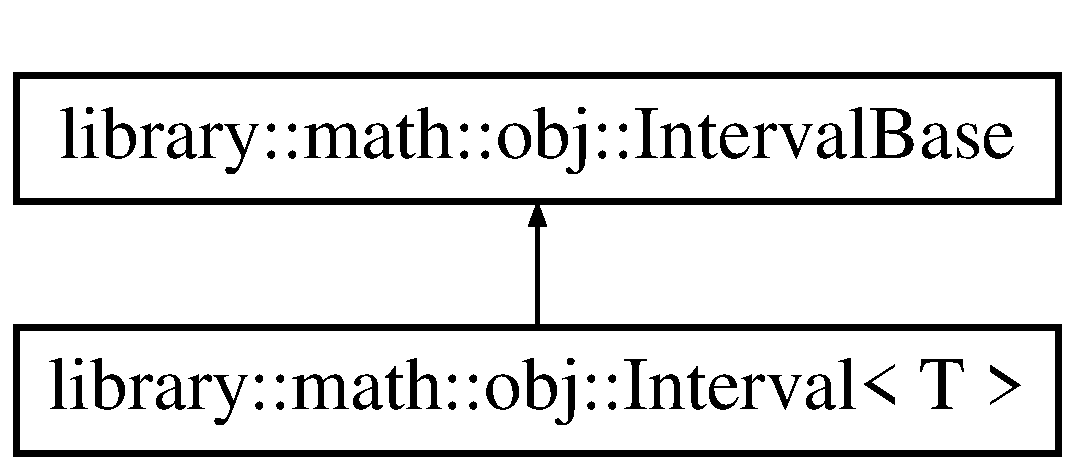
\includegraphics[height=2.000000cm]{classlibrary_1_1math_1_1obj_1_1_interval_base}
\end{center}
\end{figure}
\subsection*{Public Types}
\begin{DoxyCompactItemize}
\item 
enum \hyperlink{classlibrary_1_1math_1_1obj_1_1_interval_base_aabce6fa07a6e2e8fd3fcab5fd0d317d6}{Type} \{ \newline
\hyperlink{classlibrary_1_1math_1_1obj_1_1_interval_base_aabce6fa07a6e2e8fd3fcab5fd0d317d6aec0fc0100c4fc1ce4eea230c3dc10360}{Type\+::\+Undefined}, 
\hyperlink{classlibrary_1_1math_1_1obj_1_1_interval_base_aabce6fa07a6e2e8fd3fcab5fd0d317d6a03f4a47830f97377a35321051685071e}{Type\+::\+Closed}, 
\hyperlink{classlibrary_1_1math_1_1obj_1_1_interval_base_aabce6fa07a6e2e8fd3fcab5fd0d317d6ac3bf447eabe632720a3aa1a7ce401274}{Type\+::\+Open}, 
\hyperlink{classlibrary_1_1math_1_1obj_1_1_interval_base_aabce6fa07a6e2e8fd3fcab5fd0d317d6ab5e08f9173f660e791d3ba99ff8281d7}{Type\+::\+Half\+Open\+Left}, 
\newline
\hyperlink{classlibrary_1_1math_1_1obj_1_1_interval_base_aabce6fa07a6e2e8fd3fcab5fd0d317d6a484f1b37e0208f622a1e6f7a3ff8c2c3}{Type\+::\+Half\+Open\+Right}
 \}\begin{DoxyCompactList}\small\item\em \hyperlink{classlibrary_1_1math_1_1obj_1_1_interval}{Interval} type. \end{DoxyCompactList}
\end{DoxyCompactItemize}


\subsection{Detailed Description}
\hyperlink{classlibrary_1_1math_1_1obj_1_1_interval}{Interval} base (used to avoid having a templated enum) 

\subsection{Member Enumeration Documentation}
\mbox{\Hypertarget{classlibrary_1_1math_1_1obj_1_1_interval_base_aabce6fa07a6e2e8fd3fcab5fd0d317d6}\label{classlibrary_1_1math_1_1obj_1_1_interval_base_aabce6fa07a6e2e8fd3fcab5fd0d317d6}} 
\index{library\+::math\+::obj\+::\+Interval\+Base@{library\+::math\+::obj\+::\+Interval\+Base}!Type@{Type}}
\index{Type@{Type}!library\+::math\+::obj\+::\+Interval\+Base@{library\+::math\+::obj\+::\+Interval\+Base}}
\subsubsection{\texorpdfstring{Type}{Type}}
{\footnotesize\ttfamily enum \hyperlink{classlibrary_1_1math_1_1obj_1_1_interval_base_aabce6fa07a6e2e8fd3fcab5fd0d317d6}{library\+::math\+::obj\+::\+Interval\+Base\+::\+Type}\hspace{0.3cm}{\ttfamily [strong]}}



\hyperlink{classlibrary_1_1math_1_1obj_1_1_interval}{Interval} type. 

\begin{DoxyEnumFields}{Enumerator}
\raisebox{\heightof{T}}[0pt][0pt]{\index{Undefined@{Undefined}!library\+::math\+::obj\+::\+Interval\+Base@{library\+::math\+::obj\+::\+Interval\+Base}}\index{library\+::math\+::obj\+::\+Interval\+Base@{library\+::math\+::obj\+::\+Interval\+Base}!Undefined@{Undefined}}}\mbox{\Hypertarget{classlibrary_1_1math_1_1obj_1_1_interval_base_aabce6fa07a6e2e8fd3fcab5fd0d317d6aec0fc0100c4fc1ce4eea230c3dc10360}\label{classlibrary_1_1math_1_1obj_1_1_interval_base_aabce6fa07a6e2e8fd3fcab5fd0d317d6aec0fc0100c4fc1ce4eea230c3dc10360}} 
Undefined&Undefined interval type. \\
\hline

\raisebox{\heightof{T}}[0pt][0pt]{\index{Closed@{Closed}!library\+::math\+::obj\+::\+Interval\+Base@{library\+::math\+::obj\+::\+Interval\+Base}}\index{library\+::math\+::obj\+::\+Interval\+Base@{library\+::math\+::obj\+::\+Interval\+Base}!Closed@{Closed}}}\mbox{\Hypertarget{classlibrary_1_1math_1_1obj_1_1_interval_base_aabce6fa07a6e2e8fd3fcab5fd0d317d6a03f4a47830f97377a35321051685071e}\label{classlibrary_1_1math_1_1obj_1_1_interval_base_aabce6fa07a6e2e8fd3fcab5fd0d317d6a03f4a47830f97377a35321051685071e}} 
Closed&Closed interval type \mbox{[}a, b\mbox{]}. \\
\hline

\raisebox{\heightof{T}}[0pt][0pt]{\index{Open@{Open}!library\+::math\+::obj\+::\+Interval\+Base@{library\+::math\+::obj\+::\+Interval\+Base}}\index{library\+::math\+::obj\+::\+Interval\+Base@{library\+::math\+::obj\+::\+Interval\+Base}!Open@{Open}}}\mbox{\Hypertarget{classlibrary_1_1math_1_1obj_1_1_interval_base_aabce6fa07a6e2e8fd3fcab5fd0d317d6ac3bf447eabe632720a3aa1a7ce401274}\label{classlibrary_1_1math_1_1obj_1_1_interval_base_aabce6fa07a6e2e8fd3fcab5fd0d317d6ac3bf447eabe632720a3aa1a7ce401274}} 
Open&Open interval type \mbox{]}a, b\mbox{[}. \\
\hline

\raisebox{\heightof{T}}[0pt][0pt]{\index{Half\+Open\+Left@{Half\+Open\+Left}!library\+::math\+::obj\+::\+Interval\+Base@{library\+::math\+::obj\+::\+Interval\+Base}}\index{library\+::math\+::obj\+::\+Interval\+Base@{library\+::math\+::obj\+::\+Interval\+Base}!Half\+Open\+Left@{Half\+Open\+Left}}}\mbox{\Hypertarget{classlibrary_1_1math_1_1obj_1_1_interval_base_aabce6fa07a6e2e8fd3fcab5fd0d317d6ab5e08f9173f660e791d3ba99ff8281d7}\label{classlibrary_1_1math_1_1obj_1_1_interval_base_aabce6fa07a6e2e8fd3fcab5fd0d317d6ab5e08f9173f660e791d3ba99ff8281d7}} 
Half\+Open\+Left&Half-\/open left interval type \mbox{]}a, b\mbox{]}. \\
\hline

\raisebox{\heightof{T}}[0pt][0pt]{\index{Half\+Open\+Right@{Half\+Open\+Right}!library\+::math\+::obj\+::\+Interval\+Base@{library\+::math\+::obj\+::\+Interval\+Base}}\index{library\+::math\+::obj\+::\+Interval\+Base@{library\+::math\+::obj\+::\+Interval\+Base}!Half\+Open\+Right@{Half\+Open\+Right}}}\mbox{\Hypertarget{classlibrary_1_1math_1_1obj_1_1_interval_base_aabce6fa07a6e2e8fd3fcab5fd0d317d6a484f1b37e0208f622a1e6f7a3ff8c2c3}\label{classlibrary_1_1math_1_1obj_1_1_interval_base_aabce6fa07a6e2e8fd3fcab5fd0d317d6a484f1b37e0208f622a1e6f7a3ff8c2c3}} 
Half\+Open\+Right&Half-\/open right interval type \mbox{[}a, b\mbox{[}. \\
\hline

\end{DoxyEnumFields}


The documentation for this class was generated from the following file\+:\begin{DoxyCompactItemize}
\item 
include/\+Library/\+Mathematics/\+Objects/\hyperlink{_interval_8hpp}{Interval.\+hpp}\end{DoxyCompactItemize}

\hypertarget{classlibrary_1_1math_1_1geom_1_1d3_1_1objects_1_1_line}{}\section{library\+:\+:math\+:\+:geom\+:\+:d3\+:\+:objects\+:\+:Line Class Reference}
\label{classlibrary_1_1math_1_1geom_1_1d3_1_1objects_1_1_line}\index{library\+::math\+::geom\+::d3\+::objects\+::\+Line@{library\+::math\+::geom\+::d3\+::objects\+::\+Line}}


\hyperlink{classlibrary_1_1math_1_1geom_1_1d3_1_1objects_1_1_line}{Line}.  




{\ttfamily \#include $<$Line.\+hpp$>$}

Inheritance diagram for library\+:\+:math\+:\+:geom\+:\+:d3\+:\+:objects\+:\+:Line\+:\begin{figure}[H]
\begin{center}
\leavevmode
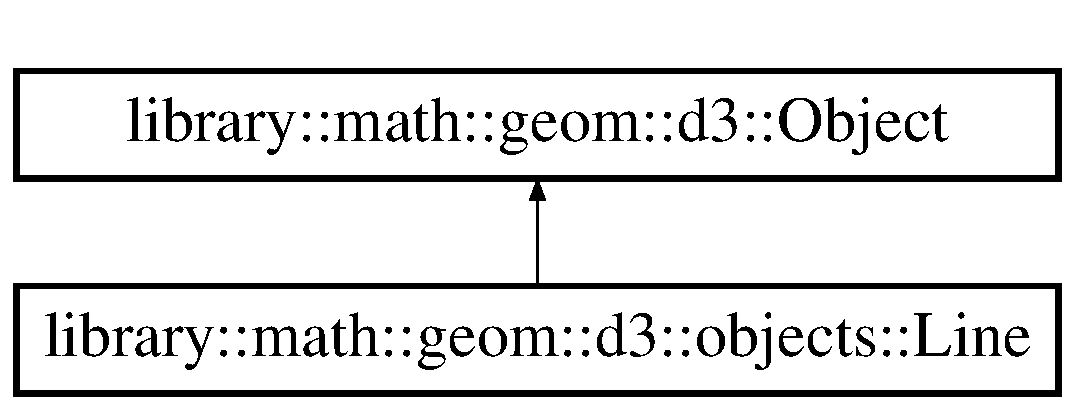
\includegraphics[height=2.000000cm]{classlibrary_1_1math_1_1geom_1_1d3_1_1objects_1_1_line}
\end{center}
\end{figure}
\subsection*{Public Member Functions}
\begin{DoxyCompactItemize}
\item 
\hyperlink{classlibrary_1_1math_1_1geom_1_1d3_1_1objects_1_1_line_a762e529453ff9ffa9233fd73737f4692}{Line} (const \hyperlink{classlibrary_1_1math_1_1geom_1_1d3_1_1objects_1_1_point}{Point} \&an\+Origin, const Vector3d \&a\+Direction)
\begin{DoxyCompactList}\small\item\em Constructor. \end{DoxyCompactList}\item 
virtual \hyperlink{classlibrary_1_1math_1_1geom_1_1d3_1_1objects_1_1_line}{Line} $\ast$ \hyperlink{classlibrary_1_1math_1_1geom_1_1d3_1_1objects_1_1_line_a55382b24007bccdae721176d0f73536f}{clone} () const override
\begin{DoxyCompactList}\small\item\em Clone line. \end{DoxyCompactList}\item 
bool \hyperlink{classlibrary_1_1math_1_1geom_1_1d3_1_1objects_1_1_line_a2e5b0da1d652abbff16d7024f8eecb0a}{operator==} (const \hyperlink{classlibrary_1_1math_1_1geom_1_1d3_1_1objects_1_1_line}{Line} \&a\+Line) const
\begin{DoxyCompactList}\small\item\em Equal to operator. \end{DoxyCompactList}\item 
bool \hyperlink{classlibrary_1_1math_1_1geom_1_1d3_1_1objects_1_1_line_ae49d3224ab2f209f192bb3b1e152766e}{operator!=} (const \hyperlink{classlibrary_1_1math_1_1geom_1_1d3_1_1objects_1_1_line}{Line} \&a\+Line) const
\begin{DoxyCompactList}\small\item\em Not equal to operator. \end{DoxyCompactList}\item 
virtual bool \hyperlink{classlibrary_1_1math_1_1geom_1_1d3_1_1objects_1_1_line_ab7b509259a32ac21c83bb14fcc7f83f3}{is\+Defined} () const override
\begin{DoxyCompactList}\small\item\em Check if line is defined. \end{DoxyCompactList}\item 
bool \hyperlink{classlibrary_1_1math_1_1geom_1_1d3_1_1objects_1_1_line_af40668ee33a6cd265a4b3c3a9a53f294}{intersects} (const \hyperlink{classlibrary_1_1math_1_1geom_1_1d3_1_1objects_1_1_point}{Point} \&a\+Point) const
\begin{DoxyCompactList}\small\item\em Check if line intersects point. \end{DoxyCompactList}\item 
bool \hyperlink{classlibrary_1_1math_1_1geom_1_1d3_1_1objects_1_1_line_ab9b35d1e6276d927e9a54219855295ce}{intersects} (const \hyperlink{classlibrary_1_1math_1_1geom_1_1d3_1_1objects_1_1_sphere}{Sphere} \&a\+Sphere) const
\begin{DoxyCompactList}\small\item\em Check if line intersects sphere. \end{DoxyCompactList}\item 
bool \hyperlink{classlibrary_1_1math_1_1geom_1_1d3_1_1objects_1_1_line_a2cc1edf1b60745c518fbf19f2ab0771c}{intersects} (const \hyperlink{classlibrary_1_1math_1_1geom_1_1d3_1_1objects_1_1_ellipsoid}{Ellipsoid} \&an\+Ellipsoid) const
\begin{DoxyCompactList}\small\item\em Check if line intersects ellipsoid. \end{DoxyCompactList}\item 
bool \hyperlink{classlibrary_1_1math_1_1geom_1_1d3_1_1objects_1_1_line_a59b72a3a39134963f5165a03829b17aa}{contains} (const \hyperlink{classlibrary_1_1math_1_1geom_1_1d3_1_1objects_1_1_point}{Point} \&a\+Point) const
\begin{DoxyCompactList}\small\item\em Check if line contains point. \end{DoxyCompactList}\item 
\hyperlink{classlibrary_1_1math_1_1geom_1_1d3_1_1objects_1_1_point}{Point} \hyperlink{classlibrary_1_1math_1_1geom_1_1d3_1_1objects_1_1_line_ad65178573d705ad21bdd54e7f4b7f104}{get\+Origin} () const
\begin{DoxyCompactList}\small\item\em Get line origin. \end{DoxyCompactList}\item 
Vector3d \hyperlink{classlibrary_1_1math_1_1geom_1_1d3_1_1objects_1_1_line_aa108a53227e4326188fe17a03c55f9cb}{get\+Direction} () const
\begin{DoxyCompactList}\small\item\em Get line direction. \end{DoxyCompactList}\item 
virtual void \hyperlink{classlibrary_1_1math_1_1geom_1_1d3_1_1objects_1_1_line_a6c2d2268fed2b9c461730fbcd4425d6e}{print} (std\+::ostream \&an\+Output\+Stream, bool display\+Decorators=true) const override
\begin{DoxyCompactList}\small\item\em Print line. \end{DoxyCompactList}\item 
virtual void \hyperlink{classlibrary_1_1math_1_1geom_1_1d3_1_1objects_1_1_line_ae485ab541cbd10113eac30d1956fb4c0}{apply\+Transformation} (const \hyperlink{classlibrary_1_1math_1_1geom_1_1d3_1_1_transformation}{Transformation} \&a\+Transformation) override
\begin{DoxyCompactList}\small\item\em Apply transformation to line. \end{DoxyCompactList}\end{DoxyCompactItemize}
\subsection*{Static Public Member Functions}
\begin{DoxyCompactItemize}
\item 
static \hyperlink{classlibrary_1_1math_1_1geom_1_1d3_1_1objects_1_1_line}{Line} \hyperlink{classlibrary_1_1math_1_1geom_1_1d3_1_1objects_1_1_line_a6e80b434196ee84bc74154532989c18c}{Undefined} ()
\begin{DoxyCompactList}\small\item\em Constructs an undefined line. \end{DoxyCompactList}\end{DoxyCompactItemize}


\subsection{Detailed Description}
\hyperlink{classlibrary_1_1math_1_1geom_1_1d3_1_1objects_1_1_line}{Line}. 

https\+://en.wikipedia.\+org/wiki/\+Line\+\_\+(geometry) 

\subsection{Constructor \& Destructor Documentation}
\mbox{\Hypertarget{classlibrary_1_1math_1_1geom_1_1d3_1_1objects_1_1_line_a762e529453ff9ffa9233fd73737f4692}\label{classlibrary_1_1math_1_1geom_1_1d3_1_1objects_1_1_line_a762e529453ff9ffa9233fd73737f4692}} 
\index{library\+::math\+::geom\+::d3\+::objects\+::\+Line@{library\+::math\+::geom\+::d3\+::objects\+::\+Line}!Line@{Line}}
\index{Line@{Line}!library\+::math\+::geom\+::d3\+::objects\+::\+Line@{library\+::math\+::geom\+::d3\+::objects\+::\+Line}}
\subsubsection{\texorpdfstring{Line()}{Line()}}
{\footnotesize\ttfamily library\+::math\+::geom\+::d3\+::objects\+::\+Line\+::\+Line (\begin{DoxyParamCaption}\item[{const \hyperlink{classlibrary_1_1math_1_1geom_1_1d3_1_1objects_1_1_point}{Point} \&}]{an\+Origin,  }\item[{const Vector3d \&}]{a\+Direction }\end{DoxyParamCaption})}



Constructor. 


\begin{DoxyCode}
\hyperlink{classlibrary_1_1math_1_1geom_1_1d3_1_1objects_1_1_line_a762e529453ff9ffa9233fd73737f4692}{Line} line(\{ 0.0, 0.0, 0.0 \}, \{ 0.0, 0.0, 1.0 \}) ;
\end{DoxyCode}



\begin{DoxyParams}[1]{Parameters}
\mbox{\tt in}  & {\em an\+Origin} & A line origin \\
\hline
\mbox{\tt in}  & {\em a\+Direction} & A line direction \\
\hline
\end{DoxyParams}


\subsection{Member Function Documentation}
\mbox{\Hypertarget{classlibrary_1_1math_1_1geom_1_1d3_1_1objects_1_1_line_ae485ab541cbd10113eac30d1956fb4c0}\label{classlibrary_1_1math_1_1geom_1_1d3_1_1objects_1_1_line_ae485ab541cbd10113eac30d1956fb4c0}} 
\index{library\+::math\+::geom\+::d3\+::objects\+::\+Line@{library\+::math\+::geom\+::d3\+::objects\+::\+Line}!apply\+Transformation@{apply\+Transformation}}
\index{apply\+Transformation@{apply\+Transformation}!library\+::math\+::geom\+::d3\+::objects\+::\+Line@{library\+::math\+::geom\+::d3\+::objects\+::\+Line}}
\subsubsection{\texorpdfstring{apply\+Transformation()}{applyTransformation()}}
{\footnotesize\ttfamily void library\+::math\+::geom\+::d3\+::objects\+::\+Line\+::apply\+Transformation (\begin{DoxyParamCaption}\item[{const \hyperlink{classlibrary_1_1math_1_1geom_1_1d3_1_1_transformation}{Transformation} \&}]{a\+Transformation }\end{DoxyParamCaption})\hspace{0.3cm}{\ttfamily [override]}, {\ttfamily [virtual]}}



Apply transformation to line. 


\begin{DoxyParams}[1]{Parameters}
\mbox{\tt in}  & {\em a\+Transformation} & A transformation \\
\hline
\end{DoxyParams}


Implements \hyperlink{classlibrary_1_1math_1_1geom_1_1d3_1_1_object_a5fc47b1ee5d9a28efc6010d3d1512470}{library\+::math\+::geom\+::d3\+::\+Object}.

\mbox{\Hypertarget{classlibrary_1_1math_1_1geom_1_1d3_1_1objects_1_1_line_a55382b24007bccdae721176d0f73536f}\label{classlibrary_1_1math_1_1geom_1_1d3_1_1objects_1_1_line_a55382b24007bccdae721176d0f73536f}} 
\index{library\+::math\+::geom\+::d3\+::objects\+::\+Line@{library\+::math\+::geom\+::d3\+::objects\+::\+Line}!clone@{clone}}
\index{clone@{clone}!library\+::math\+::geom\+::d3\+::objects\+::\+Line@{library\+::math\+::geom\+::d3\+::objects\+::\+Line}}
\subsubsection{\texorpdfstring{clone()}{clone()}}
{\footnotesize\ttfamily \hyperlink{classlibrary_1_1math_1_1geom_1_1d3_1_1objects_1_1_line}{Line} $\ast$ library\+::math\+::geom\+::d3\+::objects\+::\+Line\+::clone (\begin{DoxyParamCaption}{ }\end{DoxyParamCaption}) const\hspace{0.3cm}{\ttfamily [override]}, {\ttfamily [virtual]}}



Clone line. 

\begin{DoxyReturn}{Returns}
Pointer to cloned line 
\end{DoxyReturn}


Implements \hyperlink{classlibrary_1_1math_1_1geom_1_1d3_1_1_object_a1a784c6b359e0eb97cd34fabc42f2f3f}{library\+::math\+::geom\+::d3\+::\+Object}.

\mbox{\Hypertarget{classlibrary_1_1math_1_1geom_1_1d3_1_1objects_1_1_line_a59b72a3a39134963f5165a03829b17aa}\label{classlibrary_1_1math_1_1geom_1_1d3_1_1objects_1_1_line_a59b72a3a39134963f5165a03829b17aa}} 
\index{library\+::math\+::geom\+::d3\+::objects\+::\+Line@{library\+::math\+::geom\+::d3\+::objects\+::\+Line}!contains@{contains}}
\index{contains@{contains}!library\+::math\+::geom\+::d3\+::objects\+::\+Line@{library\+::math\+::geom\+::d3\+::objects\+::\+Line}}
\subsubsection{\texorpdfstring{contains()}{contains()}}
{\footnotesize\ttfamily bool library\+::math\+::geom\+::d3\+::objects\+::\+Line\+::contains (\begin{DoxyParamCaption}\item[{const \hyperlink{classlibrary_1_1math_1_1geom_1_1d3_1_1objects_1_1_point}{Point} \&}]{a\+Point }\end{DoxyParamCaption}) const}



Check if line contains point. 


\begin{DoxyCode}
\hyperlink{classlibrary_1_1math_1_1geom_1_1d3_1_1objects_1_1_line_a762e529453ff9ffa9233fd73737f4692}{Line} line = ... ;
Ellipsoid ellipsoid = ... ;
line.contains(ellipsoid) ;
\end{DoxyCode}



\begin{DoxyParams}[1]{Parameters}
\mbox{\tt in}  & {\em an\+Ellipsoid} & An ellipsoid \\
\hline
\end{DoxyParams}
\begin{DoxyReturn}{Returns}
True if line contains point 
\end{DoxyReturn}
\mbox{\Hypertarget{classlibrary_1_1math_1_1geom_1_1d3_1_1objects_1_1_line_aa108a53227e4326188fe17a03c55f9cb}\label{classlibrary_1_1math_1_1geom_1_1d3_1_1objects_1_1_line_aa108a53227e4326188fe17a03c55f9cb}} 
\index{library\+::math\+::geom\+::d3\+::objects\+::\+Line@{library\+::math\+::geom\+::d3\+::objects\+::\+Line}!get\+Direction@{get\+Direction}}
\index{get\+Direction@{get\+Direction}!library\+::math\+::geom\+::d3\+::objects\+::\+Line@{library\+::math\+::geom\+::d3\+::objects\+::\+Line}}
\subsubsection{\texorpdfstring{get\+Direction()}{getDirection()}}
{\footnotesize\ttfamily Vector3d library\+::math\+::geom\+::d3\+::objects\+::\+Line\+::get\+Direction (\begin{DoxyParamCaption}{ }\end{DoxyParamCaption}) const}



Get line direction. 


\begin{DoxyCode}
\hyperlink{classlibrary_1_1math_1_1geom_1_1d3_1_1objects_1_1_line_a762e529453ff9ffa9233fd73737f4692}{Line}(\{ 0.0, 0.0, 0.0 \}, \{ 0.0, 0.0, 1.0 \}).\hyperlink{classlibrary_1_1math_1_1geom_1_1d3_1_1objects_1_1_line_aa108a53227e4326188fe17a03c55f9cb}{getDirection}() ; \textcolor{comment}{// [0.0, 0.0, 1.0]}
\end{DoxyCode}


\begin{DoxyReturn}{Returns}
\hyperlink{classlibrary_1_1math_1_1geom_1_1d3_1_1objects_1_1_line}{Line} direction 
\end{DoxyReturn}
\mbox{\Hypertarget{classlibrary_1_1math_1_1geom_1_1d3_1_1objects_1_1_line_ad65178573d705ad21bdd54e7f4b7f104}\label{classlibrary_1_1math_1_1geom_1_1d3_1_1objects_1_1_line_ad65178573d705ad21bdd54e7f4b7f104}} 
\index{library\+::math\+::geom\+::d3\+::objects\+::\+Line@{library\+::math\+::geom\+::d3\+::objects\+::\+Line}!get\+Origin@{get\+Origin}}
\index{get\+Origin@{get\+Origin}!library\+::math\+::geom\+::d3\+::objects\+::\+Line@{library\+::math\+::geom\+::d3\+::objects\+::\+Line}}
\subsubsection{\texorpdfstring{get\+Origin()}{getOrigin()}}
{\footnotesize\ttfamily \hyperlink{classlibrary_1_1math_1_1geom_1_1d3_1_1objects_1_1_point}{Point} library\+::math\+::geom\+::d3\+::objects\+::\+Line\+::get\+Origin (\begin{DoxyParamCaption}{ }\end{DoxyParamCaption}) const}



Get line origin. 


\begin{DoxyCode}
\hyperlink{classlibrary_1_1math_1_1geom_1_1d3_1_1objects_1_1_line_a762e529453ff9ffa9233fd73737f4692}{Line}(\{ 0.0, 0.0, 0.0 \}, \{ 0.0, 0.0, 1.0 \}).\hyperlink{classlibrary_1_1math_1_1geom_1_1d3_1_1objects_1_1_line_ad65178573d705ad21bdd54e7f4b7f104}{getOrigin}() ; \textcolor{comment}{// [0.0, 0.0, 0.0]}
\end{DoxyCode}


\begin{DoxyReturn}{Returns}
\hyperlink{classlibrary_1_1math_1_1geom_1_1d3_1_1objects_1_1_line}{Line} origin 
\end{DoxyReturn}
\mbox{\Hypertarget{classlibrary_1_1math_1_1geom_1_1d3_1_1objects_1_1_line_af40668ee33a6cd265a4b3c3a9a53f294}\label{classlibrary_1_1math_1_1geom_1_1d3_1_1objects_1_1_line_af40668ee33a6cd265a4b3c3a9a53f294}} 
\index{library\+::math\+::geom\+::d3\+::objects\+::\+Line@{library\+::math\+::geom\+::d3\+::objects\+::\+Line}!intersects@{intersects}}
\index{intersects@{intersects}!library\+::math\+::geom\+::d3\+::objects\+::\+Line@{library\+::math\+::geom\+::d3\+::objects\+::\+Line}}
\subsubsection{\texorpdfstring{intersects()}{intersects()}\hspace{0.1cm}{\footnotesize\ttfamily [1/3]}}
{\footnotesize\ttfamily bool library\+::math\+::geom\+::d3\+::objects\+::\+Line\+::intersects (\begin{DoxyParamCaption}\item[{const \hyperlink{classlibrary_1_1math_1_1geom_1_1d3_1_1objects_1_1_point}{Point} \&}]{a\+Point }\end{DoxyParamCaption}) const}



Check if line intersects point. 


\begin{DoxyCode}
\hyperlink{classlibrary_1_1math_1_1geom_1_1d3_1_1objects_1_1_line_a762e529453ff9ffa9233fd73737f4692}{Line} line = ... ;
Point point = ... ;
line.intersects(point) ;
\end{DoxyCode}



\begin{DoxyParams}[1]{Parameters}
\mbox{\tt in}  & {\em an\+Point} & An point \\
\hline
\end{DoxyParams}
\begin{DoxyReturn}{Returns}
True if line intersects point 
\end{DoxyReturn}
\mbox{\Hypertarget{classlibrary_1_1math_1_1geom_1_1d3_1_1objects_1_1_line_ab9b35d1e6276d927e9a54219855295ce}\label{classlibrary_1_1math_1_1geom_1_1d3_1_1objects_1_1_line_ab9b35d1e6276d927e9a54219855295ce}} 
\index{library\+::math\+::geom\+::d3\+::objects\+::\+Line@{library\+::math\+::geom\+::d3\+::objects\+::\+Line}!intersects@{intersects}}
\index{intersects@{intersects}!library\+::math\+::geom\+::d3\+::objects\+::\+Line@{library\+::math\+::geom\+::d3\+::objects\+::\+Line}}
\subsubsection{\texorpdfstring{intersects()}{intersects()}\hspace{0.1cm}{\footnotesize\ttfamily [2/3]}}
{\footnotesize\ttfamily bool library\+::math\+::geom\+::d3\+::objects\+::\+Line\+::intersects (\begin{DoxyParamCaption}\item[{const \hyperlink{classlibrary_1_1math_1_1geom_1_1d3_1_1objects_1_1_sphere}{Sphere} \&}]{a\+Sphere }\end{DoxyParamCaption}) const}



Check if line intersects sphere. 


\begin{DoxyCode}
\hyperlink{classlibrary_1_1math_1_1geom_1_1d3_1_1objects_1_1_line_a762e529453ff9ffa9233fd73737f4692}{Line} line = ... ;
Sphere sphere = ... ;
line.intersects(sphere) ;
\end{DoxyCode}



\begin{DoxyParams}[1]{Parameters}
\mbox{\tt in}  & {\em a\+Sphere} & A sphere \\
\hline
\end{DoxyParams}
\begin{DoxyReturn}{Returns}
True if line intersects sphere 
\end{DoxyReturn}
\mbox{\Hypertarget{classlibrary_1_1math_1_1geom_1_1d3_1_1objects_1_1_line_a2cc1edf1b60745c518fbf19f2ab0771c}\label{classlibrary_1_1math_1_1geom_1_1d3_1_1objects_1_1_line_a2cc1edf1b60745c518fbf19f2ab0771c}} 
\index{library\+::math\+::geom\+::d3\+::objects\+::\+Line@{library\+::math\+::geom\+::d3\+::objects\+::\+Line}!intersects@{intersects}}
\index{intersects@{intersects}!library\+::math\+::geom\+::d3\+::objects\+::\+Line@{library\+::math\+::geom\+::d3\+::objects\+::\+Line}}
\subsubsection{\texorpdfstring{intersects()}{intersects()}\hspace{0.1cm}{\footnotesize\ttfamily [3/3]}}
{\footnotesize\ttfamily bool library\+::math\+::geom\+::d3\+::objects\+::\+Line\+::intersects (\begin{DoxyParamCaption}\item[{const \hyperlink{classlibrary_1_1math_1_1geom_1_1d3_1_1objects_1_1_ellipsoid}{Ellipsoid} \&}]{an\+Ellipsoid }\end{DoxyParamCaption}) const}



Check if line intersects ellipsoid. 


\begin{DoxyCode}
\hyperlink{classlibrary_1_1math_1_1geom_1_1d3_1_1objects_1_1_line_a762e529453ff9ffa9233fd73737f4692}{Line} line = ... ;
Ellipsoid ellipsoid = ... ;
line.intersects(ellipsoid) ;
\end{DoxyCode}



\begin{DoxyParams}[1]{Parameters}
\mbox{\tt in}  & {\em an\+Ellipsoid} & An ellipsoid \\
\hline
\end{DoxyParams}
\begin{DoxyReturn}{Returns}
True if line intersects ellipsoid 
\end{DoxyReturn}
\mbox{\Hypertarget{classlibrary_1_1math_1_1geom_1_1d3_1_1objects_1_1_line_ab7b509259a32ac21c83bb14fcc7f83f3}\label{classlibrary_1_1math_1_1geom_1_1d3_1_1objects_1_1_line_ab7b509259a32ac21c83bb14fcc7f83f3}} 
\index{library\+::math\+::geom\+::d3\+::objects\+::\+Line@{library\+::math\+::geom\+::d3\+::objects\+::\+Line}!is\+Defined@{is\+Defined}}
\index{is\+Defined@{is\+Defined}!library\+::math\+::geom\+::d3\+::objects\+::\+Line@{library\+::math\+::geom\+::d3\+::objects\+::\+Line}}
\subsubsection{\texorpdfstring{is\+Defined()}{isDefined()}}
{\footnotesize\ttfamily bool library\+::math\+::geom\+::d3\+::objects\+::\+Line\+::is\+Defined (\begin{DoxyParamCaption}{ }\end{DoxyParamCaption}) const\hspace{0.3cm}{\ttfamily [override]}, {\ttfamily [virtual]}}



Check if line is defined. 


\begin{DoxyCode}
\hyperlink{classlibrary_1_1math_1_1geom_1_1d3_1_1objects_1_1_line_a762e529453ff9ffa9233fd73737f4692}{Line}(\{ 0.0, 0.0, 0.0 \}, \{ 0.0, 0.0, 1.0 \}).\hyperlink{classlibrary_1_1math_1_1geom_1_1d3_1_1objects_1_1_line_ab7b509259a32ac21c83bb14fcc7f83f3}{isDefined}() ; \textcolor{comment}{// True}
\end{DoxyCode}


\begin{DoxyReturn}{Returns}
True if line is defined 
\end{DoxyReturn}


Implements \hyperlink{classlibrary_1_1math_1_1geom_1_1d3_1_1_object_a2216442e322f0c3ca5f01a4efa22baf7}{library\+::math\+::geom\+::d3\+::\+Object}.

\mbox{\Hypertarget{classlibrary_1_1math_1_1geom_1_1d3_1_1objects_1_1_line_ae49d3224ab2f209f192bb3b1e152766e}\label{classlibrary_1_1math_1_1geom_1_1d3_1_1objects_1_1_line_ae49d3224ab2f209f192bb3b1e152766e}} 
\index{library\+::math\+::geom\+::d3\+::objects\+::\+Line@{library\+::math\+::geom\+::d3\+::objects\+::\+Line}!operator"!=@{operator"!=}}
\index{operator"!=@{operator"!=}!library\+::math\+::geom\+::d3\+::objects\+::\+Line@{library\+::math\+::geom\+::d3\+::objects\+::\+Line}}
\subsubsection{\texorpdfstring{operator"!=()}{operator!=()}}
{\footnotesize\ttfamily bool library\+::math\+::geom\+::d3\+::objects\+::\+Line\+::operator!= (\begin{DoxyParamCaption}\item[{const \hyperlink{classlibrary_1_1math_1_1geom_1_1d3_1_1objects_1_1_line}{Line} \&}]{a\+Line }\end{DoxyParamCaption}) const}



Not equal to operator. 


\begin{DoxyCode}
\hyperlink{classlibrary_1_1math_1_1geom_1_1d3_1_1objects_1_1_line_a762e529453ff9ffa9233fd73737f4692}{Line}(\{ 0.0, 0.0, 0.0 \}, \{ 0.0, 0.0, 1.0 \}) != \hyperlink{classlibrary_1_1math_1_1geom_1_1d3_1_1objects_1_1_line_a762e529453ff9ffa9233fd73737f4692}{Line}(\{ 0.0, 0.0, 0.0 \}, \{ 0.0, 0.0, 2.0 \}) ; \textcolor{comment}{// True}
\end{DoxyCode}



\begin{DoxyParams}[1]{Parameters}
\mbox{\tt in}  & {\em a\+Line} & A line \\
\hline
\end{DoxyParams}
\begin{DoxyReturn}{Returns}
True if lines are not equal 
\end{DoxyReturn}
\mbox{\Hypertarget{classlibrary_1_1math_1_1geom_1_1d3_1_1objects_1_1_line_a2e5b0da1d652abbff16d7024f8eecb0a}\label{classlibrary_1_1math_1_1geom_1_1d3_1_1objects_1_1_line_a2e5b0da1d652abbff16d7024f8eecb0a}} 
\index{library\+::math\+::geom\+::d3\+::objects\+::\+Line@{library\+::math\+::geom\+::d3\+::objects\+::\+Line}!operator==@{operator==}}
\index{operator==@{operator==}!library\+::math\+::geom\+::d3\+::objects\+::\+Line@{library\+::math\+::geom\+::d3\+::objects\+::\+Line}}
\subsubsection{\texorpdfstring{operator==()}{operator==()}}
{\footnotesize\ttfamily bool library\+::math\+::geom\+::d3\+::objects\+::\+Line\+::operator== (\begin{DoxyParamCaption}\item[{const \hyperlink{classlibrary_1_1math_1_1geom_1_1d3_1_1objects_1_1_line}{Line} \&}]{a\+Line }\end{DoxyParamCaption}) const}



Equal to operator. 


\begin{DoxyCode}
\hyperlink{classlibrary_1_1math_1_1geom_1_1d3_1_1objects_1_1_line_a762e529453ff9ffa9233fd73737f4692}{Line}(\{ 0.0, 0.0, 0.0 \}, \{ 0.0, 0.0, 1.0 \}) == \hyperlink{classlibrary_1_1math_1_1geom_1_1d3_1_1objects_1_1_line_a762e529453ff9ffa9233fd73737f4692}{Line}(\{ 0.0, 0.0, 0.0 \}, \{ 0.0, 0.0, 1.0 \}) ; \textcolor{comment}{// True}
\end{DoxyCode}



\begin{DoxyParams}[1]{Parameters}
\mbox{\tt in}  & {\em a\+Line} & A line \\
\hline
\end{DoxyParams}
\begin{DoxyReturn}{Returns}
True if lines are equal 
\end{DoxyReturn}
\mbox{\Hypertarget{classlibrary_1_1math_1_1geom_1_1d3_1_1objects_1_1_line_a6c2d2268fed2b9c461730fbcd4425d6e}\label{classlibrary_1_1math_1_1geom_1_1d3_1_1objects_1_1_line_a6c2d2268fed2b9c461730fbcd4425d6e}} 
\index{library\+::math\+::geom\+::d3\+::objects\+::\+Line@{library\+::math\+::geom\+::d3\+::objects\+::\+Line}!print@{print}}
\index{print@{print}!library\+::math\+::geom\+::d3\+::objects\+::\+Line@{library\+::math\+::geom\+::d3\+::objects\+::\+Line}}
\subsubsection{\texorpdfstring{print()}{print()}}
{\footnotesize\ttfamily void library\+::math\+::geom\+::d3\+::objects\+::\+Line\+::print (\begin{DoxyParamCaption}\item[{std\+::ostream \&}]{an\+Output\+Stream,  }\item[{bool}]{display\+Decorators = {\ttfamily true} }\end{DoxyParamCaption}) const\hspace{0.3cm}{\ttfamily [override]}, {\ttfamily [virtual]}}



Print line. 


\begin{DoxyParams}[1]{Parameters}
\mbox{\tt in}  & {\em an\+Output\+Stream} & An output stream \\
\hline
\mbox{\tt in}  & {\em (optional)} & display\+Decorators If true, display decorators \\
\hline
\end{DoxyParams}


Implements \hyperlink{classlibrary_1_1math_1_1geom_1_1d3_1_1_object_aa166f4ce4d116a248f0fc861c75012ca}{library\+::math\+::geom\+::d3\+::\+Object}.

\mbox{\Hypertarget{classlibrary_1_1math_1_1geom_1_1d3_1_1objects_1_1_line_a6e80b434196ee84bc74154532989c18c}\label{classlibrary_1_1math_1_1geom_1_1d3_1_1objects_1_1_line_a6e80b434196ee84bc74154532989c18c}} 
\index{library\+::math\+::geom\+::d3\+::objects\+::\+Line@{library\+::math\+::geom\+::d3\+::objects\+::\+Line}!Undefined@{Undefined}}
\index{Undefined@{Undefined}!library\+::math\+::geom\+::d3\+::objects\+::\+Line@{library\+::math\+::geom\+::d3\+::objects\+::\+Line}}
\subsubsection{\texorpdfstring{Undefined()}{Undefined()}}
{\footnotesize\ttfamily \hyperlink{classlibrary_1_1math_1_1geom_1_1d3_1_1objects_1_1_line}{Line} library\+::math\+::geom\+::d3\+::objects\+::\+Line\+::\+Undefined (\begin{DoxyParamCaption}{ }\end{DoxyParamCaption})\hspace{0.3cm}{\ttfamily [static]}}



Constructs an undefined line. 


\begin{DoxyCode}
\hyperlink{classlibrary_1_1math_1_1geom_1_1d3_1_1objects_1_1_line_a762e529453ff9ffa9233fd73737f4692}{Line} line = \hyperlink{classlibrary_1_1math_1_1geom_1_1d3_1_1objects_1_1_line_a6e80b434196ee84bc74154532989c18c}{Line::Undefined}() ; \textcolor{comment}{// Undefined}
\end{DoxyCode}


\begin{DoxyReturn}{Returns}
Undefined line 
\end{DoxyReturn}


The documentation for this class was generated from the following files\+:\begin{DoxyCompactItemize}
\item 
include/\+Library/\+Mathematics/\+Geometry/3\+D/\+Objects/\hyperlink{_line_8hpp}{Line.\+hpp}\item 
src/\+Library/\+Mathematics/\+Geometry/3\+D/\+Objects/\hyperlink{_line_8cpp}{Line.\+cpp}\end{DoxyCompactItemize}

\hypertarget{classlibrary_1_1math_1_1geom_1_1d3_1_1objects_1_1_line_string}{}\section{library\+:\+:math\+:\+:geom\+:\+:d3\+:\+:objects\+:\+:Line\+String Class Reference}
\label{classlibrary_1_1math_1_1geom_1_1d3_1_1objects_1_1_line_string}\index{library\+::math\+::geom\+::d3\+::objects\+::\+Line\+String@{library\+::math\+::geom\+::d3\+::objects\+::\+Line\+String}}


\hyperlink{classlibrary_1_1math_1_1geom_1_1d3_1_1objects_1_1_line}{Line} string.  




{\ttfamily \#include $<$Line\+String.\+hpp$>$}

Inheritance diagram for library\+:\+:math\+:\+:geom\+:\+:d3\+:\+:objects\+:\+:Line\+String\+:\begin{figure}[H]
\begin{center}
\leavevmode
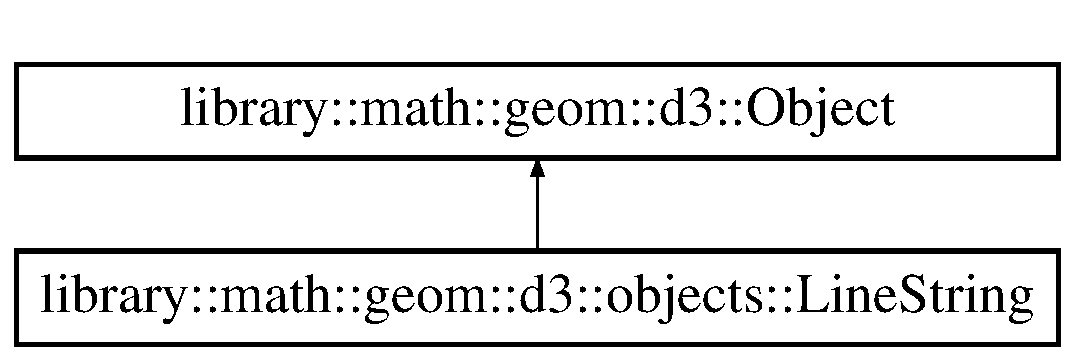
\includegraphics[height=2.000000cm]{classlibrary_1_1math_1_1geom_1_1d3_1_1objects_1_1_line_string}
\end{center}
\end{figure}
\subsection*{Public Types}
\begin{DoxyCompactItemize}
\item 
typedef Array$<$ \hyperlink{classlibrary_1_1math_1_1geom_1_1d3_1_1objects_1_1_point}{Point} $>$\+::\hyperlink{classlibrary_1_1math_1_1geom_1_1d3_1_1objects_1_1_line_string_a87db0104282f9fcccdc5b1b99e2301e5}{Const\+Iterator} \hyperlink{classlibrary_1_1math_1_1geom_1_1d3_1_1objects_1_1_line_string_a87db0104282f9fcccdc5b1b99e2301e5}{Const\+Iterator}
\end{DoxyCompactItemize}
\subsection*{Public Member Functions}
\begin{DoxyCompactItemize}
\item 
\hyperlink{classlibrary_1_1math_1_1geom_1_1d3_1_1objects_1_1_line_string_aab80e60f34f06d4ab9f84f0e59aa389e}{Line\+String} (const Array$<$ \hyperlink{classlibrary_1_1math_1_1geom_1_1d3_1_1objects_1_1_point}{Point} $>$ \&a\+Point\+Array)
\begin{DoxyCompactList}\small\item\em Constructor. \end{DoxyCompactList}\item 
virtual \hyperlink{classlibrary_1_1math_1_1geom_1_1d3_1_1objects_1_1_line_string}{Line\+String} $\ast$ \hyperlink{classlibrary_1_1math_1_1geom_1_1d3_1_1objects_1_1_line_string_a95ef100ab7053589b845980ca4c845b3}{clone} () const override
\begin{DoxyCompactList}\small\item\em Clone line string. \end{DoxyCompactList}\item 
bool \hyperlink{classlibrary_1_1math_1_1geom_1_1d3_1_1objects_1_1_line_string_ab413b3ed8f6f78697420f6c4c3b4d0e6}{operator==} (const \hyperlink{classlibrary_1_1math_1_1geom_1_1d3_1_1objects_1_1_line_string}{Line\+String} \&a\+Line\+String) const
\begin{DoxyCompactList}\small\item\em Equal to operator. \end{DoxyCompactList}\item 
bool \hyperlink{classlibrary_1_1math_1_1geom_1_1d3_1_1objects_1_1_line_string_a9702b88a1713fcace96a34840ab5d1d2}{operator!=} (const \hyperlink{classlibrary_1_1math_1_1geom_1_1d3_1_1objects_1_1_line_string}{Line\+String} \&a\+Line\+String) const
\begin{DoxyCompactList}\small\item\em Not equal to operator. \end{DoxyCompactList}\item 
virtual bool \hyperlink{classlibrary_1_1math_1_1geom_1_1d3_1_1objects_1_1_line_string_a310ff5c1068792e92b58bcda8e72dfec}{is\+Defined} () const override
\begin{DoxyCompactList}\small\item\em Check if line string is defined. \end{DoxyCompactList}\item 
bool \hyperlink{classlibrary_1_1math_1_1geom_1_1d3_1_1objects_1_1_line_string_a33e1e2dfcd7352eb41b6991bd97ec6cd}{is\+Empty} () const
\begin{DoxyCompactList}\small\item\em Check if line string is empty. \end{DoxyCompactList}\item 
bool \hyperlink{classlibrary_1_1math_1_1geom_1_1d3_1_1objects_1_1_line_string_acbfb3f1c542793b9fa810ba8626633c4}{is\+Near} (const \hyperlink{classlibrary_1_1math_1_1geom_1_1d3_1_1objects_1_1_line_string}{Line\+String} \&a\+Line\+String, const Real \&a\+Tolerance) const
\begin{DoxyCompactList}\small\item\em Check if line string is near another line string. \end{DoxyCompactList}\item 
const \hyperlink{classlibrary_1_1math_1_1geom_1_1d3_1_1objects_1_1_point}{Point} \& \hyperlink{classlibrary_1_1math_1_1geom_1_1d3_1_1objects_1_1_line_string_a10bafe20bf12505dfe7dfb9c83ce1613}{access\+Point\+At} (const Index \&an\+Index) const
\begin{DoxyCompactList}\small\item\em Access point at index. \end{DoxyCompactList}\item 
Size \hyperlink{classlibrary_1_1math_1_1geom_1_1d3_1_1objects_1_1_line_string_ac635c796406d38f6f1019b64cab9b42c}{get\+Point\+Count} () const
\begin{DoxyCompactList}\small\item\em Get point count. \end{DoxyCompactList}\item 
\hyperlink{classlibrary_1_1math_1_1geom_1_1d3_1_1objects_1_1_point}{Point} \hyperlink{classlibrary_1_1math_1_1geom_1_1d3_1_1objects_1_1_line_string_a39cf8a2be15c3f1686ed855659ded104}{get\+Point\+Closest\+To} (const \hyperlink{classlibrary_1_1math_1_1geom_1_1d3_1_1objects_1_1_point}{Point} \&a\+Point) const
\begin{DoxyCompactList}\small\item\em Get point closest to another point. \end{DoxyCompactList}\item 
virtual void \hyperlink{classlibrary_1_1math_1_1geom_1_1d3_1_1objects_1_1_line_string_a289414dbfc4ff32520f546c8a435170f}{print} (std\+::ostream \&an\+Output\+Stream, bool display\+Decorators=true) const override
\begin{DoxyCompactList}\small\item\em Print point. \end{DoxyCompactList}\item 
\hyperlink{classlibrary_1_1math_1_1geom_1_1d3_1_1objects_1_1_line_string_a87db0104282f9fcccdc5b1b99e2301e5}{Line\+String\+::\+Const\+Iterator} \hyperlink{classlibrary_1_1math_1_1geom_1_1d3_1_1objects_1_1_line_string_a218630b02ea7a4f32872fd1ee25f3359}{begin} () const
\begin{DoxyCompactList}\small\item\em Get begin const iterator. \end{DoxyCompactList}\item 
\hyperlink{classlibrary_1_1math_1_1geom_1_1d3_1_1objects_1_1_line_string_a87db0104282f9fcccdc5b1b99e2301e5}{Line\+String\+::\+Const\+Iterator} \hyperlink{classlibrary_1_1math_1_1geom_1_1d3_1_1objects_1_1_line_string_a83d9d9ba96fc956a900a7cd2dbf3e82b}{end} () const
\begin{DoxyCompactList}\small\item\em Get end const iterator. \end{DoxyCompactList}\item 
virtual void \hyperlink{classlibrary_1_1math_1_1geom_1_1d3_1_1objects_1_1_line_string_a8a20f45b2af9cc45dbf7aff9e5d4824e}{apply\+Transformation} (const \hyperlink{classlibrary_1_1math_1_1geom_1_1d3_1_1_transformation}{Transformation} \&a\+Transformation) override
\begin{DoxyCompactList}\small\item\em Apply transformation to line string. \end{DoxyCompactList}\end{DoxyCompactItemize}
\subsection*{Static Public Member Functions}
\begin{DoxyCompactItemize}
\item 
static \hyperlink{classlibrary_1_1math_1_1geom_1_1d3_1_1objects_1_1_line_string}{Line\+String} \hyperlink{classlibrary_1_1math_1_1geom_1_1d3_1_1objects_1_1_line_string_ae9e05ddb3ab59060c78d18e19624f307}{Empty} ()
\begin{DoxyCompactList}\small\item\em Constructs an empty line string. \end{DoxyCompactList}\item 
static \hyperlink{classlibrary_1_1math_1_1geom_1_1d3_1_1objects_1_1_line_string}{Line\+String} \hyperlink{classlibrary_1_1math_1_1geom_1_1d3_1_1objects_1_1_line_string_a7fb1bcb80907e72aa55f0692ed2517f1}{Segment} (const \hyperlink{classlibrary_1_1math_1_1geom_1_1d3_1_1objects_1_1_segment}{objects\+::\+Segment} \&a\+Segment)
\begin{DoxyCompactList}\small\item\em Constructs a line string from a segment. \end{DoxyCompactList}\end{DoxyCompactItemize}


\subsection{Detailed Description}
\hyperlink{classlibrary_1_1math_1_1geom_1_1d3_1_1objects_1_1_line}{Line} string. 

\subsection{Member Typedef Documentation}
\mbox{\Hypertarget{classlibrary_1_1math_1_1geom_1_1d3_1_1objects_1_1_line_string_a87db0104282f9fcccdc5b1b99e2301e5}\label{classlibrary_1_1math_1_1geom_1_1d3_1_1objects_1_1_line_string_a87db0104282f9fcccdc5b1b99e2301e5}} 
\index{library\+::math\+::geom\+::d3\+::objects\+::\+Line\+String@{library\+::math\+::geom\+::d3\+::objects\+::\+Line\+String}!Const\+Iterator@{Const\+Iterator}}
\index{Const\+Iterator@{Const\+Iterator}!library\+::math\+::geom\+::d3\+::objects\+::\+Line\+String@{library\+::math\+::geom\+::d3\+::objects\+::\+Line\+String}}
\subsubsection{\texorpdfstring{Const\+Iterator}{ConstIterator}}
{\footnotesize\ttfamily typedef Array$<$\hyperlink{classlibrary_1_1math_1_1geom_1_1d3_1_1objects_1_1_point}{Point}$>$\+::\hyperlink{classlibrary_1_1math_1_1geom_1_1d3_1_1objects_1_1_line_string_a87db0104282f9fcccdc5b1b99e2301e5}{Const\+Iterator} \hyperlink{classlibrary_1_1math_1_1geom_1_1d3_1_1objects_1_1_line_string_a87db0104282f9fcccdc5b1b99e2301e5}{library\+::math\+::geom\+::d3\+::objects\+::\+Line\+String\+::\+Const\+Iterator}}



\subsection{Constructor \& Destructor Documentation}
\mbox{\Hypertarget{classlibrary_1_1math_1_1geom_1_1d3_1_1objects_1_1_line_string_aab80e60f34f06d4ab9f84f0e59aa389e}\label{classlibrary_1_1math_1_1geom_1_1d3_1_1objects_1_1_line_string_aab80e60f34f06d4ab9f84f0e59aa389e}} 
\index{library\+::math\+::geom\+::d3\+::objects\+::\+Line\+String@{library\+::math\+::geom\+::d3\+::objects\+::\+Line\+String}!Line\+String@{Line\+String}}
\index{Line\+String@{Line\+String}!library\+::math\+::geom\+::d3\+::objects\+::\+Line\+String@{library\+::math\+::geom\+::d3\+::objects\+::\+Line\+String}}
\subsubsection{\texorpdfstring{Line\+String()}{LineString()}}
{\footnotesize\ttfamily library\+::math\+::geom\+::d3\+::objects\+::\+Line\+String\+::\+Line\+String (\begin{DoxyParamCaption}\item[{const Array$<$ \hyperlink{classlibrary_1_1math_1_1geom_1_1d3_1_1objects_1_1_point}{Point} $>$ \&}]{a\+Point\+Array }\end{DoxyParamCaption})}



Constructor. 


\begin{DoxyCode}
\hyperlink{classlibrary_1_1math_1_1geom_1_1d3_1_1objects_1_1_line_string_aab80e60f34f06d4ab9f84f0e59aa389e}{LineString} lineString(\{ \{ 0.0, 0.0, 0.0 \}, \{ 0.0, 1.0, 0.0 \}, \{ 1.0, 0.0, 1.0 \} \}) ;
\end{DoxyCode}



\begin{DoxyParams}[1]{Parameters}
\mbox{\tt in}  & {\em a\+Point\+Array} & A point array \\
\hline
\end{DoxyParams}


\subsection{Member Function Documentation}
\mbox{\Hypertarget{classlibrary_1_1math_1_1geom_1_1d3_1_1objects_1_1_line_string_a10bafe20bf12505dfe7dfb9c83ce1613}\label{classlibrary_1_1math_1_1geom_1_1d3_1_1objects_1_1_line_string_a10bafe20bf12505dfe7dfb9c83ce1613}} 
\index{library\+::math\+::geom\+::d3\+::objects\+::\+Line\+String@{library\+::math\+::geom\+::d3\+::objects\+::\+Line\+String}!access\+Point\+At@{access\+Point\+At}}
\index{access\+Point\+At@{access\+Point\+At}!library\+::math\+::geom\+::d3\+::objects\+::\+Line\+String@{library\+::math\+::geom\+::d3\+::objects\+::\+Line\+String}}
\subsubsection{\texorpdfstring{access\+Point\+At()}{accessPointAt()}}
{\footnotesize\ttfamily const \hyperlink{classlibrary_1_1math_1_1geom_1_1d3_1_1objects_1_1_point}{Point} \& library\+::math\+::geom\+::d3\+::objects\+::\+Line\+String\+::access\+Point\+At (\begin{DoxyParamCaption}\item[{const Index \&}]{an\+Index }\end{DoxyParamCaption}) const}



Access point at index. 

\mbox{[}in\mbox{]} an\+Index A point index \begin{DoxyReturn}{Returns}
Reference to point at index 
\end{DoxyReturn}
\mbox{\Hypertarget{classlibrary_1_1math_1_1geom_1_1d3_1_1objects_1_1_line_string_a8a20f45b2af9cc45dbf7aff9e5d4824e}\label{classlibrary_1_1math_1_1geom_1_1d3_1_1objects_1_1_line_string_a8a20f45b2af9cc45dbf7aff9e5d4824e}} 
\index{library\+::math\+::geom\+::d3\+::objects\+::\+Line\+String@{library\+::math\+::geom\+::d3\+::objects\+::\+Line\+String}!apply\+Transformation@{apply\+Transformation}}
\index{apply\+Transformation@{apply\+Transformation}!library\+::math\+::geom\+::d3\+::objects\+::\+Line\+String@{library\+::math\+::geom\+::d3\+::objects\+::\+Line\+String}}
\subsubsection{\texorpdfstring{apply\+Transformation()}{applyTransformation()}}
{\footnotesize\ttfamily void library\+::math\+::geom\+::d3\+::objects\+::\+Line\+String\+::apply\+Transformation (\begin{DoxyParamCaption}\item[{const \hyperlink{classlibrary_1_1math_1_1geom_1_1d3_1_1_transformation}{Transformation} \&}]{a\+Transformation }\end{DoxyParamCaption})\hspace{0.3cm}{\ttfamily [override]}, {\ttfamily [virtual]}}



Apply transformation to line string. 


\begin{DoxyParams}[1]{Parameters}
\mbox{\tt in}  & {\em a\+Transformation} & A transformation \\
\hline
\end{DoxyParams}


Implements \hyperlink{classlibrary_1_1math_1_1geom_1_1d3_1_1_object_a5fc47b1ee5d9a28efc6010d3d1512470}{library\+::math\+::geom\+::d3\+::\+Object}.

\mbox{\Hypertarget{classlibrary_1_1math_1_1geom_1_1d3_1_1objects_1_1_line_string_a218630b02ea7a4f32872fd1ee25f3359}\label{classlibrary_1_1math_1_1geom_1_1d3_1_1objects_1_1_line_string_a218630b02ea7a4f32872fd1ee25f3359}} 
\index{library\+::math\+::geom\+::d3\+::objects\+::\+Line\+String@{library\+::math\+::geom\+::d3\+::objects\+::\+Line\+String}!begin@{begin}}
\index{begin@{begin}!library\+::math\+::geom\+::d3\+::objects\+::\+Line\+String@{library\+::math\+::geom\+::d3\+::objects\+::\+Line\+String}}
\subsubsection{\texorpdfstring{begin()}{begin()}}
{\footnotesize\ttfamily \hyperlink{classlibrary_1_1math_1_1geom_1_1d3_1_1objects_1_1_line_string_a87db0104282f9fcccdc5b1b99e2301e5}{Line\+String\+::\+Const\+Iterator} library\+::math\+::geom\+::d3\+::objects\+::\+Line\+String\+::begin (\begin{DoxyParamCaption}{ }\end{DoxyParamCaption}) const}



Get begin const iterator. 

\begin{DoxyReturn}{Returns}
Begin const iterator 
\end{DoxyReturn}
\mbox{\Hypertarget{classlibrary_1_1math_1_1geom_1_1d3_1_1objects_1_1_line_string_a95ef100ab7053589b845980ca4c845b3}\label{classlibrary_1_1math_1_1geom_1_1d3_1_1objects_1_1_line_string_a95ef100ab7053589b845980ca4c845b3}} 
\index{library\+::math\+::geom\+::d3\+::objects\+::\+Line\+String@{library\+::math\+::geom\+::d3\+::objects\+::\+Line\+String}!clone@{clone}}
\index{clone@{clone}!library\+::math\+::geom\+::d3\+::objects\+::\+Line\+String@{library\+::math\+::geom\+::d3\+::objects\+::\+Line\+String}}
\subsubsection{\texorpdfstring{clone()}{clone()}}
{\footnotesize\ttfamily \hyperlink{classlibrary_1_1math_1_1geom_1_1d3_1_1objects_1_1_line_string}{Line\+String} $\ast$ library\+::math\+::geom\+::d3\+::objects\+::\+Line\+String\+::clone (\begin{DoxyParamCaption}{ }\end{DoxyParamCaption}) const\hspace{0.3cm}{\ttfamily [override]}, {\ttfamily [virtual]}}



Clone line string. 

\begin{DoxyReturn}{Returns}
Pointer to cloned line string 
\end{DoxyReturn}


Implements \hyperlink{classlibrary_1_1math_1_1geom_1_1d3_1_1_object_a1a784c6b359e0eb97cd34fabc42f2f3f}{library\+::math\+::geom\+::d3\+::\+Object}.

\mbox{\Hypertarget{classlibrary_1_1math_1_1geom_1_1d3_1_1objects_1_1_line_string_ae9e05ddb3ab59060c78d18e19624f307}\label{classlibrary_1_1math_1_1geom_1_1d3_1_1objects_1_1_line_string_ae9e05ddb3ab59060c78d18e19624f307}} 
\index{library\+::math\+::geom\+::d3\+::objects\+::\+Line\+String@{library\+::math\+::geom\+::d3\+::objects\+::\+Line\+String}!Empty@{Empty}}
\index{Empty@{Empty}!library\+::math\+::geom\+::d3\+::objects\+::\+Line\+String@{library\+::math\+::geom\+::d3\+::objects\+::\+Line\+String}}
\subsubsection{\texorpdfstring{Empty()}{Empty()}}
{\footnotesize\ttfamily \hyperlink{classlibrary_1_1math_1_1geom_1_1d3_1_1objects_1_1_line_string}{Line\+String} library\+::math\+::geom\+::d3\+::objects\+::\+Line\+String\+::\+Empty (\begin{DoxyParamCaption}{ }\end{DoxyParamCaption})\hspace{0.3cm}{\ttfamily [static]}}



Constructs an empty line string. 


\begin{DoxyCode}
\hyperlink{classlibrary_1_1math_1_1geom_1_1d3_1_1objects_1_1_line_string_aab80e60f34f06d4ab9f84f0e59aa389e}{LineString} lineString = \hyperlink{classlibrary_1_1math_1_1geom_1_1d3_1_1objects_1_1_line_string_ae9e05ddb3ab59060c78d18e19624f307}{LineString::Empty}() ;
\end{DoxyCode}


\begin{DoxyReturn}{Returns}
Empty line string 
\end{DoxyReturn}
\mbox{\Hypertarget{classlibrary_1_1math_1_1geom_1_1d3_1_1objects_1_1_line_string_a83d9d9ba96fc956a900a7cd2dbf3e82b}\label{classlibrary_1_1math_1_1geom_1_1d3_1_1objects_1_1_line_string_a83d9d9ba96fc956a900a7cd2dbf3e82b}} 
\index{library\+::math\+::geom\+::d3\+::objects\+::\+Line\+String@{library\+::math\+::geom\+::d3\+::objects\+::\+Line\+String}!end@{end}}
\index{end@{end}!library\+::math\+::geom\+::d3\+::objects\+::\+Line\+String@{library\+::math\+::geom\+::d3\+::objects\+::\+Line\+String}}
\subsubsection{\texorpdfstring{end()}{end()}}
{\footnotesize\ttfamily \hyperlink{classlibrary_1_1math_1_1geom_1_1d3_1_1objects_1_1_line_string_a87db0104282f9fcccdc5b1b99e2301e5}{Line\+String\+::\+Const\+Iterator} library\+::math\+::geom\+::d3\+::objects\+::\+Line\+String\+::end (\begin{DoxyParamCaption}{ }\end{DoxyParamCaption}) const}



Get end const iterator. 

\begin{DoxyReturn}{Returns}
End const iterator 
\end{DoxyReturn}
\mbox{\Hypertarget{classlibrary_1_1math_1_1geom_1_1d3_1_1objects_1_1_line_string_a39cf8a2be15c3f1686ed855659ded104}\label{classlibrary_1_1math_1_1geom_1_1d3_1_1objects_1_1_line_string_a39cf8a2be15c3f1686ed855659ded104}} 
\index{library\+::math\+::geom\+::d3\+::objects\+::\+Line\+String@{library\+::math\+::geom\+::d3\+::objects\+::\+Line\+String}!get\+Point\+Closest\+To@{get\+Point\+Closest\+To}}
\index{get\+Point\+Closest\+To@{get\+Point\+Closest\+To}!library\+::math\+::geom\+::d3\+::objects\+::\+Line\+String@{library\+::math\+::geom\+::d3\+::objects\+::\+Line\+String}}
\subsubsection{\texorpdfstring{get\+Point\+Closest\+To()}{getPointClosestTo()}}
{\footnotesize\ttfamily \hyperlink{classlibrary_1_1math_1_1geom_1_1d3_1_1objects_1_1_point}{Point} library\+::math\+::geom\+::d3\+::objects\+::\+Line\+String\+::get\+Point\+Closest\+To (\begin{DoxyParamCaption}\item[{const \hyperlink{classlibrary_1_1math_1_1geom_1_1d3_1_1objects_1_1_point}{Point} \&}]{a\+Point }\end{DoxyParamCaption}) const}



Get point closest to another point. 


\begin{DoxyParams}[1]{Parameters}
\mbox{\tt in}  & {\em a\+Point} & A point \\
\hline
\end{DoxyParams}
\begin{DoxyReturn}{Returns}
Closest point 
\end{DoxyReturn}
\mbox{\Hypertarget{classlibrary_1_1math_1_1geom_1_1d3_1_1objects_1_1_line_string_ac635c796406d38f6f1019b64cab9b42c}\label{classlibrary_1_1math_1_1geom_1_1d3_1_1objects_1_1_line_string_ac635c796406d38f6f1019b64cab9b42c}} 
\index{library\+::math\+::geom\+::d3\+::objects\+::\+Line\+String@{library\+::math\+::geom\+::d3\+::objects\+::\+Line\+String}!get\+Point\+Count@{get\+Point\+Count}}
\index{get\+Point\+Count@{get\+Point\+Count}!library\+::math\+::geom\+::d3\+::objects\+::\+Line\+String@{library\+::math\+::geom\+::d3\+::objects\+::\+Line\+String}}
\subsubsection{\texorpdfstring{get\+Point\+Count()}{getPointCount()}}
{\footnotesize\ttfamily Size library\+::math\+::geom\+::d3\+::objects\+::\+Line\+String\+::get\+Point\+Count (\begin{DoxyParamCaption}{ }\end{DoxyParamCaption}) const}



Get point count. 

\begin{DoxyReturn}{Returns}
\hyperlink{classlibrary_1_1math_1_1geom_1_1d3_1_1objects_1_1_point}{Point} count 
\end{DoxyReturn}
\mbox{\Hypertarget{classlibrary_1_1math_1_1geom_1_1d3_1_1objects_1_1_line_string_a310ff5c1068792e92b58bcda8e72dfec}\label{classlibrary_1_1math_1_1geom_1_1d3_1_1objects_1_1_line_string_a310ff5c1068792e92b58bcda8e72dfec}} 
\index{library\+::math\+::geom\+::d3\+::objects\+::\+Line\+String@{library\+::math\+::geom\+::d3\+::objects\+::\+Line\+String}!is\+Defined@{is\+Defined}}
\index{is\+Defined@{is\+Defined}!library\+::math\+::geom\+::d3\+::objects\+::\+Line\+String@{library\+::math\+::geom\+::d3\+::objects\+::\+Line\+String}}
\subsubsection{\texorpdfstring{is\+Defined()}{isDefined()}}
{\footnotesize\ttfamily bool library\+::math\+::geom\+::d3\+::objects\+::\+Line\+String\+::is\+Defined (\begin{DoxyParamCaption}{ }\end{DoxyParamCaption}) const\hspace{0.3cm}{\ttfamily [override]}, {\ttfamily [virtual]}}



Check if line string is defined. 


\begin{DoxyCode}
\hyperlink{classlibrary_1_1math_1_1geom_1_1d3_1_1objects_1_1_line_string_aab80e60f34f06d4ab9f84f0e59aa389e}{LineString}(0.0, 0.0).isDefined() ; \textcolor{comment}{// True}
\end{DoxyCode}


\begin{DoxyReturn}{Returns}
True if line string is defined 
\end{DoxyReturn}


Implements \hyperlink{classlibrary_1_1math_1_1geom_1_1d3_1_1_object_a2216442e322f0c3ca5f01a4efa22baf7}{library\+::math\+::geom\+::d3\+::\+Object}.

\mbox{\Hypertarget{classlibrary_1_1math_1_1geom_1_1d3_1_1objects_1_1_line_string_a33e1e2dfcd7352eb41b6991bd97ec6cd}\label{classlibrary_1_1math_1_1geom_1_1d3_1_1objects_1_1_line_string_a33e1e2dfcd7352eb41b6991bd97ec6cd}} 
\index{library\+::math\+::geom\+::d3\+::objects\+::\+Line\+String@{library\+::math\+::geom\+::d3\+::objects\+::\+Line\+String}!is\+Empty@{is\+Empty}}
\index{is\+Empty@{is\+Empty}!library\+::math\+::geom\+::d3\+::objects\+::\+Line\+String@{library\+::math\+::geom\+::d3\+::objects\+::\+Line\+String}}
\subsubsection{\texorpdfstring{is\+Empty()}{isEmpty()}}
{\footnotesize\ttfamily bool library\+::math\+::geom\+::d3\+::objects\+::\+Line\+String\+::is\+Empty (\begin{DoxyParamCaption}{ }\end{DoxyParamCaption}) const}



Check if line string is empty. 


\begin{DoxyCode}
\hyperlink{classlibrary_1_1math_1_1geom_1_1d3_1_1objects_1_1_line_string_ae9e05ddb3ab59060c78d18e19624f307}{LineString::Empty}().\hyperlink{classlibrary_1_1math_1_1geom_1_1d3_1_1objects_1_1_line_string_a33e1e2dfcd7352eb41b6991bd97ec6cd}{isEmpty}() ; \textcolor{comment}{// True}
\end{DoxyCode}


\begin{DoxyReturn}{Returns}
True if line string is empty 
\end{DoxyReturn}
\mbox{\Hypertarget{classlibrary_1_1math_1_1geom_1_1d3_1_1objects_1_1_line_string_acbfb3f1c542793b9fa810ba8626633c4}\label{classlibrary_1_1math_1_1geom_1_1d3_1_1objects_1_1_line_string_acbfb3f1c542793b9fa810ba8626633c4}} 
\index{library\+::math\+::geom\+::d3\+::objects\+::\+Line\+String@{library\+::math\+::geom\+::d3\+::objects\+::\+Line\+String}!is\+Near@{is\+Near}}
\index{is\+Near@{is\+Near}!library\+::math\+::geom\+::d3\+::objects\+::\+Line\+String@{library\+::math\+::geom\+::d3\+::objects\+::\+Line\+String}}
\subsubsection{\texorpdfstring{is\+Near()}{isNear()}}
{\footnotesize\ttfamily bool library\+::math\+::geom\+::d3\+::objects\+::\+Line\+String\+::is\+Near (\begin{DoxyParamCaption}\item[{const \hyperlink{classlibrary_1_1math_1_1geom_1_1d3_1_1objects_1_1_line_string}{Line\+String} \&}]{a\+Line\+String,  }\item[{const Real \&}]{a\+Tolerance }\end{DoxyParamCaption}) const}



Check if line string is near another line string. 


\begin{DoxyCode}
\hyperlink{classlibrary_1_1math_1_1geom_1_1d3_1_1objects_1_1_line_string_aab80e60f34f06d4ab9f84f0e59aa389e}{LineString}(\{ \{ 0.0, 0.0, 0.0 \}, \{ 0.0, 1.0, 0.0 \}, \{ 1.0, 0.0, 1.0 \} \}).
      \hyperlink{classlibrary_1_1math_1_1geom_1_1d3_1_1objects_1_1_line_string_acbfb3f1c542793b9fa810ba8626633c4}{isNear}(\hyperlink{classlibrary_1_1math_1_1geom_1_1d3_1_1objects_1_1_line_string_aab80e60f34f06d4ab9f84f0e59aa389e}{LineString}(\{ \{ 0.0, 0.0, 0.0 \}, \{ 0.0, 1.0, 1e-15 \}, \{ 1.0, 0.0, 1.0 \} \}), 1e-15) ; \textcolor{comment}{
      // True}
\end{DoxyCode}



\begin{DoxyParams}[1]{Parameters}
\mbox{\tt in}  & {\em a\+Line\+String} & A line string \\
\hline
\mbox{\tt in}  & {\em a\+Tolerance} & A tolerance \\
\hline
\end{DoxyParams}
\begin{DoxyReturn}{Returns}
True if line string is near another line string 
\end{DoxyReturn}
\mbox{\Hypertarget{classlibrary_1_1math_1_1geom_1_1d3_1_1objects_1_1_line_string_a9702b88a1713fcace96a34840ab5d1d2}\label{classlibrary_1_1math_1_1geom_1_1d3_1_1objects_1_1_line_string_a9702b88a1713fcace96a34840ab5d1d2}} 
\index{library\+::math\+::geom\+::d3\+::objects\+::\+Line\+String@{library\+::math\+::geom\+::d3\+::objects\+::\+Line\+String}!operator"!=@{operator"!=}}
\index{operator"!=@{operator"!=}!library\+::math\+::geom\+::d3\+::objects\+::\+Line\+String@{library\+::math\+::geom\+::d3\+::objects\+::\+Line\+String}}
\subsubsection{\texorpdfstring{operator"!=()}{operator!=()}}
{\footnotesize\ttfamily bool library\+::math\+::geom\+::d3\+::objects\+::\+Line\+String\+::operator!= (\begin{DoxyParamCaption}\item[{const \hyperlink{classlibrary_1_1math_1_1geom_1_1d3_1_1objects_1_1_line_string}{Line\+String} \&}]{a\+Line\+String }\end{DoxyParamCaption}) const}



Not equal to operator. 


\begin{DoxyParams}[1]{Parameters}
\mbox{\tt in}  & {\em a\+Line\+String} & A line string \\
\hline
\end{DoxyParams}
\begin{DoxyReturn}{Returns}
True if line strings are not equal 
\end{DoxyReturn}
\mbox{\Hypertarget{classlibrary_1_1math_1_1geom_1_1d3_1_1objects_1_1_line_string_ab413b3ed8f6f78697420f6c4c3b4d0e6}\label{classlibrary_1_1math_1_1geom_1_1d3_1_1objects_1_1_line_string_ab413b3ed8f6f78697420f6c4c3b4d0e6}} 
\index{library\+::math\+::geom\+::d3\+::objects\+::\+Line\+String@{library\+::math\+::geom\+::d3\+::objects\+::\+Line\+String}!operator==@{operator==}}
\index{operator==@{operator==}!library\+::math\+::geom\+::d3\+::objects\+::\+Line\+String@{library\+::math\+::geom\+::d3\+::objects\+::\+Line\+String}}
\subsubsection{\texorpdfstring{operator==()}{operator==()}}
{\footnotesize\ttfamily bool library\+::math\+::geom\+::d3\+::objects\+::\+Line\+String\+::operator== (\begin{DoxyParamCaption}\item[{const \hyperlink{classlibrary_1_1math_1_1geom_1_1d3_1_1objects_1_1_line_string}{Line\+String} \&}]{a\+Line\+String }\end{DoxyParamCaption}) const}



Equal to operator. 


\begin{DoxyParams}[1]{Parameters}
\mbox{\tt in}  & {\em a\+Line\+String} & A line string \\
\hline
\end{DoxyParams}
\begin{DoxyReturn}{Returns}
True if line strings are equal 
\end{DoxyReturn}
\mbox{\Hypertarget{classlibrary_1_1math_1_1geom_1_1d3_1_1objects_1_1_line_string_a289414dbfc4ff32520f546c8a435170f}\label{classlibrary_1_1math_1_1geom_1_1d3_1_1objects_1_1_line_string_a289414dbfc4ff32520f546c8a435170f}} 
\index{library\+::math\+::geom\+::d3\+::objects\+::\+Line\+String@{library\+::math\+::geom\+::d3\+::objects\+::\+Line\+String}!print@{print}}
\index{print@{print}!library\+::math\+::geom\+::d3\+::objects\+::\+Line\+String@{library\+::math\+::geom\+::d3\+::objects\+::\+Line\+String}}
\subsubsection{\texorpdfstring{print()}{print()}}
{\footnotesize\ttfamily void library\+::math\+::geom\+::d3\+::objects\+::\+Line\+String\+::print (\begin{DoxyParamCaption}\item[{std\+::ostream \&}]{an\+Output\+Stream,  }\item[{bool}]{display\+Decorators = {\ttfamily true} }\end{DoxyParamCaption}) const\hspace{0.3cm}{\ttfamily [override]}, {\ttfamily [virtual]}}



Print point. 


\begin{DoxyParams}[1]{Parameters}
\mbox{\tt in}  & {\em an\+Output\+Stream} & An output stream \\
\hline
\mbox{\tt in}  & {\em (optional)} & display\+Decorators If true, display decorators \\
\hline
\end{DoxyParams}


Implements \hyperlink{classlibrary_1_1math_1_1geom_1_1d3_1_1_object_aa166f4ce4d116a248f0fc861c75012ca}{library\+::math\+::geom\+::d3\+::\+Object}.

\mbox{\Hypertarget{classlibrary_1_1math_1_1geom_1_1d3_1_1objects_1_1_line_string_a7fb1bcb80907e72aa55f0692ed2517f1}\label{classlibrary_1_1math_1_1geom_1_1d3_1_1objects_1_1_line_string_a7fb1bcb80907e72aa55f0692ed2517f1}} 
\index{library\+::math\+::geom\+::d3\+::objects\+::\+Line\+String@{library\+::math\+::geom\+::d3\+::objects\+::\+Line\+String}!Segment@{Segment}}
\index{Segment@{Segment}!library\+::math\+::geom\+::d3\+::objects\+::\+Line\+String@{library\+::math\+::geom\+::d3\+::objects\+::\+Line\+String}}
\subsubsection{\texorpdfstring{Segment()}{Segment()}}
{\footnotesize\ttfamily \hyperlink{classlibrary_1_1math_1_1geom_1_1d3_1_1objects_1_1_line_string}{Line\+String} library\+::math\+::geom\+::d3\+::objects\+::\+Line\+String\+::\+Segment (\begin{DoxyParamCaption}\item[{const \hyperlink{classlibrary_1_1math_1_1geom_1_1d3_1_1objects_1_1_segment}{objects\+::\+Segment} \&}]{a\+Segment }\end{DoxyParamCaption})\hspace{0.3cm}{\ttfamily [static]}}



Constructs a line string from a segment. 


\begin{DoxyCode}
\hyperlink{classlibrary_1_1math_1_1geom_1_1d3_1_1objects_1_1_line_string_a7fb1bcb80907e72aa55f0692ed2517f1}{Segment} segment = \{ \{ 0.0, 0.0, 0.0 \}, \{ 0.0, 1.0, 2.0 \} \} ;
\hyperlink{classlibrary_1_1math_1_1geom_1_1d3_1_1objects_1_1_line_string_aab80e60f34f06d4ab9f84f0e59aa389e}{LineString} lineString = \hyperlink{classlibrary_1_1math_1_1geom_1_1d3_1_1objects_1_1_line_string_a7fb1bcb80907e72aa55f0692ed2517f1}{LineString::Segment}(segment) ;
\end{DoxyCode}


\begin{DoxyReturn}{Returns}
\hyperlink{classlibrary_1_1math_1_1geom_1_1d3_1_1objects_1_1_line}{Line} string 
\end{DoxyReturn}


The documentation for this class was generated from the following files\+:\begin{DoxyCompactItemize}
\item 
include/\+Library/\+Mathematics/\+Geometry/3\+D/\+Objects/\hyperlink{3_d_2_objects_2_line_string_8hpp}{Line\+String.\+hpp}\item 
src/\+Library/\+Mathematics/\+Geometry/3\+D/\+Objects/\hyperlink{3_d_2_objects_2_line_string_8cpp}{Line\+String.\+cpp}\end{DoxyCompactItemize}

\hypertarget{classlibrary_1_1math_1_1geom_1_1d2_1_1objects_1_1_line_string}{}\section{library\+:\+:math\+:\+:geom\+:\+:d2\+:\+:objects\+:\+:Line\+String Class Reference}
\label{classlibrary_1_1math_1_1geom_1_1d2_1_1objects_1_1_line_string}\index{library\+::math\+::geom\+::d2\+::objects\+::\+Line\+String@{library\+::math\+::geom\+::d2\+::objects\+::\+Line\+String}}


Line string.  




{\ttfamily \#include $<$Line\+String.\+hpp$>$}

Inheritance diagram for library\+:\+:math\+:\+:geom\+:\+:d2\+:\+:objects\+:\+:Line\+String\+:\begin{figure}[H]
\begin{center}
\leavevmode
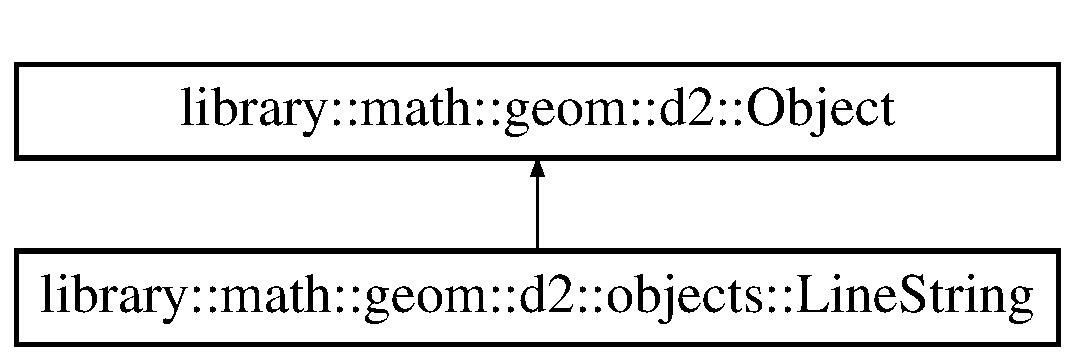
\includegraphics[height=2.000000cm]{classlibrary_1_1math_1_1geom_1_1d2_1_1objects_1_1_line_string}
\end{center}
\end{figure}
\subsection*{Public Types}
\begin{DoxyCompactItemize}
\item 
typedef Array$<$ \hyperlink{classlibrary_1_1math_1_1geom_1_1d2_1_1objects_1_1_point}{Point} $>$\+::\hyperlink{classlibrary_1_1math_1_1geom_1_1d2_1_1objects_1_1_line_string_a7c7a81b557da8ed855b5f4b88a5fa837}{Const\+Iterator} \hyperlink{classlibrary_1_1math_1_1geom_1_1d2_1_1objects_1_1_line_string_a7c7a81b557da8ed855b5f4b88a5fa837}{Const\+Iterator}
\end{DoxyCompactItemize}
\subsection*{Public Member Functions}
\begin{DoxyCompactItemize}
\item 
\hyperlink{classlibrary_1_1math_1_1geom_1_1d2_1_1objects_1_1_line_string_aa313a076051c7fb722b9eeb6d5bf2f7e}{Line\+String} (const Array$<$ \hyperlink{classlibrary_1_1math_1_1geom_1_1d2_1_1objects_1_1_point}{Point} $>$ \&a\+Point\+Array)
\begin{DoxyCompactList}\small\item\em Constructor. \end{DoxyCompactList}\item 
virtual \hyperlink{classlibrary_1_1math_1_1geom_1_1d2_1_1objects_1_1_line_string}{Line\+String} $\ast$ \hyperlink{classlibrary_1_1math_1_1geom_1_1d2_1_1objects_1_1_line_string_a5b503802b279c6c305fed6a07a893ad2}{clone} () const override
\begin{DoxyCompactList}\small\item\em Clone line string. \end{DoxyCompactList}\item 
bool \hyperlink{classlibrary_1_1math_1_1geom_1_1d2_1_1objects_1_1_line_string_a9243f1af02509aa7053d5e8ed3a4223c}{operator==} (const \hyperlink{classlibrary_1_1math_1_1geom_1_1d2_1_1objects_1_1_line_string}{Line\+String} \&a\+Line\+String) const
\begin{DoxyCompactList}\small\item\em Equal to operator. \end{DoxyCompactList}\item 
bool \hyperlink{classlibrary_1_1math_1_1geom_1_1d2_1_1objects_1_1_line_string_a4a31177281bb5be25122a70885771584}{operator!=} (const \hyperlink{classlibrary_1_1math_1_1geom_1_1d2_1_1objects_1_1_line_string}{Line\+String} \&a\+Line\+String) const
\begin{DoxyCompactList}\small\item\em Not equal to operator. \end{DoxyCompactList}\item 
virtual bool \hyperlink{classlibrary_1_1math_1_1geom_1_1d2_1_1objects_1_1_line_string_a2ef4a1e387ed463286fac7c93fd7b022}{is\+Defined} () const override
\begin{DoxyCompactList}\small\item\em Check if line string is defined. \end{DoxyCompactList}\item 
bool \hyperlink{classlibrary_1_1math_1_1geom_1_1d2_1_1objects_1_1_line_string_a4cdb4e69cd076285cb14356b86b41fcf}{is\+Empty} () const
\begin{DoxyCompactList}\small\item\em Check if line string is empty. \end{DoxyCompactList}\item 
bool \hyperlink{classlibrary_1_1math_1_1geom_1_1d2_1_1objects_1_1_line_string_a306598a5dca56802f094c57465a4d551}{is\+Near} (const \hyperlink{classlibrary_1_1math_1_1geom_1_1d2_1_1objects_1_1_line_string}{Line\+String} \&a\+Line\+String, const Real \&a\+Tolerance) const
\begin{DoxyCompactList}\small\item\em Check if line string is near another line string. \end{DoxyCompactList}\item 
const \hyperlink{classlibrary_1_1math_1_1geom_1_1d2_1_1objects_1_1_point}{Point} \& \hyperlink{classlibrary_1_1math_1_1geom_1_1d2_1_1objects_1_1_line_string_af3978277bde56a5bfec46d5f2ebd3e59}{access\+Point\+At} (const Index \&an\+Index) const
\begin{DoxyCompactList}\small\item\em Access point at index. \end{DoxyCompactList}\item 
Size \hyperlink{classlibrary_1_1math_1_1geom_1_1d2_1_1objects_1_1_line_string_a950ceda32b44a6f2e49c1e36bc4f4dc2}{get\+Point\+Count} () const
\begin{DoxyCompactList}\small\item\em Get point count. \end{DoxyCompactList}\item 
\hyperlink{classlibrary_1_1math_1_1geom_1_1d2_1_1objects_1_1_point}{Point} \hyperlink{classlibrary_1_1math_1_1geom_1_1d2_1_1objects_1_1_line_string_a038dba8bffbcaaf498a349341458db4a}{get\+Point\+Closest\+To} (const \hyperlink{classlibrary_1_1math_1_1geom_1_1d2_1_1objects_1_1_point}{Point} \&a\+Point) const
\begin{DoxyCompactList}\small\item\em Get point closest to another point. \end{DoxyCompactList}\item 
virtual String \hyperlink{classlibrary_1_1math_1_1geom_1_1d2_1_1objects_1_1_line_string_a13c0a7c5b8da7724b5a2dd2933064768}{to\+String} (const \hyperlink{classlibrary_1_1math_1_1geom_1_1d2_1_1_object_ac8cd61dada4960cfee9a469231621b17}{Object\+::\+Format} \&a\+Format=\hyperlink{classlibrary_1_1math_1_1geom_1_1d2_1_1_object_ac8cd61dada4960cfee9a469231621b17aeb6d8ae6f20283755b339c0dc273988b}{Object\+::\+Format\+::\+Standard}, const Integer \&a\+Precision=Integer\+::\+Undefined()) const override
\begin{DoxyCompactList}\small\item\em Get string representation. \end{DoxyCompactList}\item 
virtual void \hyperlink{classlibrary_1_1math_1_1geom_1_1d2_1_1objects_1_1_line_string_ae980ac86d1f2d8091151252aef2b6adc}{print} (std\+::ostream \&an\+Output\+Stream, bool display\+Decorators=true) const override
\begin{DoxyCompactList}\small\item\em Print point. \end{DoxyCompactList}\item 
\hyperlink{classlibrary_1_1math_1_1geom_1_1d2_1_1objects_1_1_line_string_a7c7a81b557da8ed855b5f4b88a5fa837}{Line\+String\+::\+Const\+Iterator} \hyperlink{classlibrary_1_1math_1_1geom_1_1d2_1_1objects_1_1_line_string_af2e6ff6ec6714eb64bda3c270c92469d}{begin} () const
\begin{DoxyCompactList}\small\item\em Get begin const iterator. \end{DoxyCompactList}\item 
\hyperlink{classlibrary_1_1math_1_1geom_1_1d2_1_1objects_1_1_line_string_a7c7a81b557da8ed855b5f4b88a5fa837}{Line\+String\+::\+Const\+Iterator} \hyperlink{classlibrary_1_1math_1_1geom_1_1d2_1_1objects_1_1_line_string_af86afe62a24b648504822b3adc6c5ecd}{end} () const
\begin{DoxyCompactList}\small\item\em Get end const iterator. \end{DoxyCompactList}\item 
virtual void \hyperlink{classlibrary_1_1math_1_1geom_1_1d2_1_1objects_1_1_line_string_abd9e77eb0e1d319e8f9af23ccb6dc0b4}{apply\+Transformation} (const \hyperlink{classlibrary_1_1math_1_1geom_1_1d2_1_1_transformation}{Transformation} \&a\+Transformation) override
\begin{DoxyCompactList}\small\item\em Apply transformation to line string. \end{DoxyCompactList}\end{DoxyCompactItemize}
\subsection*{Static Public Member Functions}
\begin{DoxyCompactItemize}
\item 
static \hyperlink{classlibrary_1_1math_1_1geom_1_1d2_1_1objects_1_1_line_string}{Line\+String} \hyperlink{classlibrary_1_1math_1_1geom_1_1d2_1_1objects_1_1_line_string_af8a783642dc4ba67d4e0ca2140cda343}{Empty} ()
\begin{DoxyCompactList}\small\item\em Constructs an empty line string. \end{DoxyCompactList}\item 
static \hyperlink{classlibrary_1_1math_1_1geom_1_1d2_1_1objects_1_1_line_string}{Line\+String} \hyperlink{classlibrary_1_1math_1_1geom_1_1d2_1_1objects_1_1_line_string_a382892044a21b1b7e2717117adef35db}{Segment} (const \hyperlink{classlibrary_1_1math_1_1geom_1_1d2_1_1objects_1_1_segment}{objects\+::\+Segment} \&a\+Segment)
\begin{DoxyCompactList}\small\item\em Constructs a line string from a segment. \end{DoxyCompactList}\end{DoxyCompactItemize}


\subsection{Detailed Description}
Line string. 

A line string is a connected series of line segments.

https\+://en.wikipedia.\+org/wiki/\+Polygonal\+\_\+chain 

\subsection{Member Typedef Documentation}
\mbox{\Hypertarget{classlibrary_1_1math_1_1geom_1_1d2_1_1objects_1_1_line_string_a7c7a81b557da8ed855b5f4b88a5fa837}\label{classlibrary_1_1math_1_1geom_1_1d2_1_1objects_1_1_line_string_a7c7a81b557da8ed855b5f4b88a5fa837}} 
\index{library\+::math\+::geom\+::d2\+::objects\+::\+Line\+String@{library\+::math\+::geom\+::d2\+::objects\+::\+Line\+String}!Const\+Iterator@{Const\+Iterator}}
\index{Const\+Iterator@{Const\+Iterator}!library\+::math\+::geom\+::d2\+::objects\+::\+Line\+String@{library\+::math\+::geom\+::d2\+::objects\+::\+Line\+String}}
\subsubsection{\texorpdfstring{Const\+Iterator}{ConstIterator}}
{\footnotesize\ttfamily typedef Array$<$\hyperlink{classlibrary_1_1math_1_1geom_1_1d2_1_1objects_1_1_point}{Point}$>$\+::\hyperlink{classlibrary_1_1math_1_1geom_1_1d2_1_1objects_1_1_line_string_a7c7a81b557da8ed855b5f4b88a5fa837}{Const\+Iterator} \hyperlink{classlibrary_1_1math_1_1geom_1_1d2_1_1objects_1_1_line_string_a7c7a81b557da8ed855b5f4b88a5fa837}{library\+::math\+::geom\+::d2\+::objects\+::\+Line\+String\+::\+Const\+Iterator}}



\subsection{Constructor \& Destructor Documentation}
\mbox{\Hypertarget{classlibrary_1_1math_1_1geom_1_1d2_1_1objects_1_1_line_string_aa313a076051c7fb722b9eeb6d5bf2f7e}\label{classlibrary_1_1math_1_1geom_1_1d2_1_1objects_1_1_line_string_aa313a076051c7fb722b9eeb6d5bf2f7e}} 
\index{library\+::math\+::geom\+::d2\+::objects\+::\+Line\+String@{library\+::math\+::geom\+::d2\+::objects\+::\+Line\+String}!Line\+String@{Line\+String}}
\index{Line\+String@{Line\+String}!library\+::math\+::geom\+::d2\+::objects\+::\+Line\+String@{library\+::math\+::geom\+::d2\+::objects\+::\+Line\+String}}
\subsubsection{\texorpdfstring{Line\+String()}{LineString()}}
{\footnotesize\ttfamily library\+::math\+::geom\+::d2\+::objects\+::\+Line\+String\+::\+Line\+String (\begin{DoxyParamCaption}\item[{const Array$<$ \hyperlink{classlibrary_1_1math_1_1geom_1_1d2_1_1objects_1_1_point}{Point} $>$ \&}]{a\+Point\+Array }\end{DoxyParamCaption})}



Constructor. 


\begin{DoxyCode}
\hyperlink{classlibrary_1_1math_1_1geom_1_1d2_1_1objects_1_1_line_string_aa313a076051c7fb722b9eeb6d5bf2f7e}{LineString} lineString(\{ \{ 0.0, 0.0 \}, \{ 0.0, 1.0 \}, \{ 1.0, 0.0 \} \}) ;
\end{DoxyCode}



\begin{DoxyParams}[1]{Parameters}
\mbox{\tt in}  & {\em a\+Point\+Array} & A point array \\
\hline
\end{DoxyParams}


\subsection{Member Function Documentation}
\mbox{\Hypertarget{classlibrary_1_1math_1_1geom_1_1d2_1_1objects_1_1_line_string_af3978277bde56a5bfec46d5f2ebd3e59}\label{classlibrary_1_1math_1_1geom_1_1d2_1_1objects_1_1_line_string_af3978277bde56a5bfec46d5f2ebd3e59}} 
\index{library\+::math\+::geom\+::d2\+::objects\+::\+Line\+String@{library\+::math\+::geom\+::d2\+::objects\+::\+Line\+String}!access\+Point\+At@{access\+Point\+At}}
\index{access\+Point\+At@{access\+Point\+At}!library\+::math\+::geom\+::d2\+::objects\+::\+Line\+String@{library\+::math\+::geom\+::d2\+::objects\+::\+Line\+String}}
\subsubsection{\texorpdfstring{access\+Point\+At()}{accessPointAt()}}
{\footnotesize\ttfamily const \hyperlink{classlibrary_1_1math_1_1geom_1_1d2_1_1objects_1_1_point}{Point} \& library\+::math\+::geom\+::d2\+::objects\+::\+Line\+String\+::access\+Point\+At (\begin{DoxyParamCaption}\item[{const Index \&}]{an\+Index }\end{DoxyParamCaption}) const}



Access point at index. 

\mbox{[}in\mbox{]} an\+Index A point index \begin{DoxyReturn}{Returns}
Reference to point at index 
\end{DoxyReturn}
\mbox{\Hypertarget{classlibrary_1_1math_1_1geom_1_1d2_1_1objects_1_1_line_string_abd9e77eb0e1d319e8f9af23ccb6dc0b4}\label{classlibrary_1_1math_1_1geom_1_1d2_1_1objects_1_1_line_string_abd9e77eb0e1d319e8f9af23ccb6dc0b4}} 
\index{library\+::math\+::geom\+::d2\+::objects\+::\+Line\+String@{library\+::math\+::geom\+::d2\+::objects\+::\+Line\+String}!apply\+Transformation@{apply\+Transformation}}
\index{apply\+Transformation@{apply\+Transformation}!library\+::math\+::geom\+::d2\+::objects\+::\+Line\+String@{library\+::math\+::geom\+::d2\+::objects\+::\+Line\+String}}
\subsubsection{\texorpdfstring{apply\+Transformation()}{applyTransformation()}}
{\footnotesize\ttfamily void library\+::math\+::geom\+::d2\+::objects\+::\+Line\+String\+::apply\+Transformation (\begin{DoxyParamCaption}\item[{const \hyperlink{classlibrary_1_1math_1_1geom_1_1d2_1_1_transformation}{Transformation} \&}]{a\+Transformation }\end{DoxyParamCaption})\hspace{0.3cm}{\ttfamily [override]}, {\ttfamily [virtual]}}



Apply transformation to line string. 


\begin{DoxyParams}[1]{Parameters}
\mbox{\tt in}  & {\em a\+Transformation} & A transformation \\
\hline
\end{DoxyParams}


Implements \hyperlink{classlibrary_1_1math_1_1geom_1_1d2_1_1_object_a289589fb6e9e7a2c4ca4976a1544def5}{library\+::math\+::geom\+::d2\+::\+Object}.

\mbox{\Hypertarget{classlibrary_1_1math_1_1geom_1_1d2_1_1objects_1_1_line_string_af2e6ff6ec6714eb64bda3c270c92469d}\label{classlibrary_1_1math_1_1geom_1_1d2_1_1objects_1_1_line_string_af2e6ff6ec6714eb64bda3c270c92469d}} 
\index{library\+::math\+::geom\+::d2\+::objects\+::\+Line\+String@{library\+::math\+::geom\+::d2\+::objects\+::\+Line\+String}!begin@{begin}}
\index{begin@{begin}!library\+::math\+::geom\+::d2\+::objects\+::\+Line\+String@{library\+::math\+::geom\+::d2\+::objects\+::\+Line\+String}}
\subsubsection{\texorpdfstring{begin()}{begin()}}
{\footnotesize\ttfamily \hyperlink{classlibrary_1_1math_1_1geom_1_1d2_1_1objects_1_1_line_string_a7c7a81b557da8ed855b5f4b88a5fa837}{Line\+String\+::\+Const\+Iterator} library\+::math\+::geom\+::d2\+::objects\+::\+Line\+String\+::begin (\begin{DoxyParamCaption}{ }\end{DoxyParamCaption}) const}



Get begin const iterator. 

\begin{DoxyReturn}{Returns}
Begin const iterator 
\end{DoxyReturn}
\mbox{\Hypertarget{classlibrary_1_1math_1_1geom_1_1d2_1_1objects_1_1_line_string_a5b503802b279c6c305fed6a07a893ad2}\label{classlibrary_1_1math_1_1geom_1_1d2_1_1objects_1_1_line_string_a5b503802b279c6c305fed6a07a893ad2}} 
\index{library\+::math\+::geom\+::d2\+::objects\+::\+Line\+String@{library\+::math\+::geom\+::d2\+::objects\+::\+Line\+String}!clone@{clone}}
\index{clone@{clone}!library\+::math\+::geom\+::d2\+::objects\+::\+Line\+String@{library\+::math\+::geom\+::d2\+::objects\+::\+Line\+String}}
\subsubsection{\texorpdfstring{clone()}{clone()}}
{\footnotesize\ttfamily \hyperlink{classlibrary_1_1math_1_1geom_1_1d2_1_1objects_1_1_line_string}{Line\+String} $\ast$ library\+::math\+::geom\+::d2\+::objects\+::\+Line\+String\+::clone (\begin{DoxyParamCaption}{ }\end{DoxyParamCaption}) const\hspace{0.3cm}{\ttfamily [override]}, {\ttfamily [virtual]}}



Clone line string. 

\begin{DoxyReturn}{Returns}
Pointer to cloned line string 
\end{DoxyReturn}


Implements \hyperlink{classlibrary_1_1math_1_1geom_1_1d2_1_1_object_a5c26ae4120edb24f6463d65a9cef247d}{library\+::math\+::geom\+::d2\+::\+Object}.

\mbox{\Hypertarget{classlibrary_1_1math_1_1geom_1_1d2_1_1objects_1_1_line_string_af8a783642dc4ba67d4e0ca2140cda343}\label{classlibrary_1_1math_1_1geom_1_1d2_1_1objects_1_1_line_string_af8a783642dc4ba67d4e0ca2140cda343}} 
\index{library\+::math\+::geom\+::d2\+::objects\+::\+Line\+String@{library\+::math\+::geom\+::d2\+::objects\+::\+Line\+String}!Empty@{Empty}}
\index{Empty@{Empty}!library\+::math\+::geom\+::d2\+::objects\+::\+Line\+String@{library\+::math\+::geom\+::d2\+::objects\+::\+Line\+String}}
\subsubsection{\texorpdfstring{Empty()}{Empty()}}
{\footnotesize\ttfamily \hyperlink{classlibrary_1_1math_1_1geom_1_1d2_1_1objects_1_1_line_string}{Line\+String} library\+::math\+::geom\+::d2\+::objects\+::\+Line\+String\+::\+Empty (\begin{DoxyParamCaption}{ }\end{DoxyParamCaption})\hspace{0.3cm}{\ttfamily [static]}}



Constructs an empty line string. 


\begin{DoxyCode}
\hyperlink{classlibrary_1_1math_1_1geom_1_1d2_1_1objects_1_1_line_string_aa313a076051c7fb722b9eeb6d5bf2f7e}{LineString} lineString = \hyperlink{classlibrary_1_1math_1_1geom_1_1d2_1_1objects_1_1_line_string_af8a783642dc4ba67d4e0ca2140cda343}{LineString::Empty}() ;
\end{DoxyCode}


\begin{DoxyReturn}{Returns}
Empty line string 
\end{DoxyReturn}
\mbox{\Hypertarget{classlibrary_1_1math_1_1geom_1_1d2_1_1objects_1_1_line_string_af86afe62a24b648504822b3adc6c5ecd}\label{classlibrary_1_1math_1_1geom_1_1d2_1_1objects_1_1_line_string_af86afe62a24b648504822b3adc6c5ecd}} 
\index{library\+::math\+::geom\+::d2\+::objects\+::\+Line\+String@{library\+::math\+::geom\+::d2\+::objects\+::\+Line\+String}!end@{end}}
\index{end@{end}!library\+::math\+::geom\+::d2\+::objects\+::\+Line\+String@{library\+::math\+::geom\+::d2\+::objects\+::\+Line\+String}}
\subsubsection{\texorpdfstring{end()}{end()}}
{\footnotesize\ttfamily \hyperlink{classlibrary_1_1math_1_1geom_1_1d2_1_1objects_1_1_line_string_a7c7a81b557da8ed855b5f4b88a5fa837}{Line\+String\+::\+Const\+Iterator} library\+::math\+::geom\+::d2\+::objects\+::\+Line\+String\+::end (\begin{DoxyParamCaption}{ }\end{DoxyParamCaption}) const}



Get end const iterator. 

\begin{DoxyReturn}{Returns}
End const iterator 
\end{DoxyReturn}
\mbox{\Hypertarget{classlibrary_1_1math_1_1geom_1_1d2_1_1objects_1_1_line_string_a038dba8bffbcaaf498a349341458db4a}\label{classlibrary_1_1math_1_1geom_1_1d2_1_1objects_1_1_line_string_a038dba8bffbcaaf498a349341458db4a}} 
\index{library\+::math\+::geom\+::d2\+::objects\+::\+Line\+String@{library\+::math\+::geom\+::d2\+::objects\+::\+Line\+String}!get\+Point\+Closest\+To@{get\+Point\+Closest\+To}}
\index{get\+Point\+Closest\+To@{get\+Point\+Closest\+To}!library\+::math\+::geom\+::d2\+::objects\+::\+Line\+String@{library\+::math\+::geom\+::d2\+::objects\+::\+Line\+String}}
\subsubsection{\texorpdfstring{get\+Point\+Closest\+To()}{getPointClosestTo()}}
{\footnotesize\ttfamily \hyperlink{classlibrary_1_1math_1_1geom_1_1d2_1_1objects_1_1_point}{Point} library\+::math\+::geom\+::d2\+::objects\+::\+Line\+String\+::get\+Point\+Closest\+To (\begin{DoxyParamCaption}\item[{const \hyperlink{classlibrary_1_1math_1_1geom_1_1d2_1_1objects_1_1_point}{Point} \&}]{a\+Point }\end{DoxyParamCaption}) const}



Get point closest to another point. 


\begin{DoxyParams}[1]{Parameters}
\mbox{\tt in}  & {\em a\+Point} & A point \\
\hline
\end{DoxyParams}
\begin{DoxyReturn}{Returns}
Closest point 
\end{DoxyReturn}
\mbox{\Hypertarget{classlibrary_1_1math_1_1geom_1_1d2_1_1objects_1_1_line_string_a950ceda32b44a6f2e49c1e36bc4f4dc2}\label{classlibrary_1_1math_1_1geom_1_1d2_1_1objects_1_1_line_string_a950ceda32b44a6f2e49c1e36bc4f4dc2}} 
\index{library\+::math\+::geom\+::d2\+::objects\+::\+Line\+String@{library\+::math\+::geom\+::d2\+::objects\+::\+Line\+String}!get\+Point\+Count@{get\+Point\+Count}}
\index{get\+Point\+Count@{get\+Point\+Count}!library\+::math\+::geom\+::d2\+::objects\+::\+Line\+String@{library\+::math\+::geom\+::d2\+::objects\+::\+Line\+String}}
\subsubsection{\texorpdfstring{get\+Point\+Count()}{getPointCount()}}
{\footnotesize\ttfamily Size library\+::math\+::geom\+::d2\+::objects\+::\+Line\+String\+::get\+Point\+Count (\begin{DoxyParamCaption}{ }\end{DoxyParamCaption}) const}



Get point count. 

\begin{DoxyReturn}{Returns}
\hyperlink{classlibrary_1_1math_1_1geom_1_1d2_1_1objects_1_1_point}{Point} count 
\end{DoxyReturn}
\mbox{\Hypertarget{classlibrary_1_1math_1_1geom_1_1d2_1_1objects_1_1_line_string_a2ef4a1e387ed463286fac7c93fd7b022}\label{classlibrary_1_1math_1_1geom_1_1d2_1_1objects_1_1_line_string_a2ef4a1e387ed463286fac7c93fd7b022}} 
\index{library\+::math\+::geom\+::d2\+::objects\+::\+Line\+String@{library\+::math\+::geom\+::d2\+::objects\+::\+Line\+String}!is\+Defined@{is\+Defined}}
\index{is\+Defined@{is\+Defined}!library\+::math\+::geom\+::d2\+::objects\+::\+Line\+String@{library\+::math\+::geom\+::d2\+::objects\+::\+Line\+String}}
\subsubsection{\texorpdfstring{is\+Defined()}{isDefined()}}
{\footnotesize\ttfamily bool library\+::math\+::geom\+::d2\+::objects\+::\+Line\+String\+::is\+Defined (\begin{DoxyParamCaption}{ }\end{DoxyParamCaption}) const\hspace{0.3cm}{\ttfamily [override]}, {\ttfamily [virtual]}}



Check if line string is defined. 


\begin{DoxyCode}
\hyperlink{classlibrary_1_1math_1_1geom_1_1d2_1_1objects_1_1_line_string_aa313a076051c7fb722b9eeb6d5bf2f7e}{LineString}(0.0, 0.0).isDefined() ; \textcolor{comment}{// True}
\end{DoxyCode}


\begin{DoxyReturn}{Returns}
True if line string is defined 
\end{DoxyReturn}


Implements \hyperlink{classlibrary_1_1math_1_1geom_1_1d2_1_1_object_ae9506254971168a3ca63e1923556b70d}{library\+::math\+::geom\+::d2\+::\+Object}.

\mbox{\Hypertarget{classlibrary_1_1math_1_1geom_1_1d2_1_1objects_1_1_line_string_a4cdb4e69cd076285cb14356b86b41fcf}\label{classlibrary_1_1math_1_1geom_1_1d2_1_1objects_1_1_line_string_a4cdb4e69cd076285cb14356b86b41fcf}} 
\index{library\+::math\+::geom\+::d2\+::objects\+::\+Line\+String@{library\+::math\+::geom\+::d2\+::objects\+::\+Line\+String}!is\+Empty@{is\+Empty}}
\index{is\+Empty@{is\+Empty}!library\+::math\+::geom\+::d2\+::objects\+::\+Line\+String@{library\+::math\+::geom\+::d2\+::objects\+::\+Line\+String}}
\subsubsection{\texorpdfstring{is\+Empty()}{isEmpty()}}
{\footnotesize\ttfamily bool library\+::math\+::geom\+::d2\+::objects\+::\+Line\+String\+::is\+Empty (\begin{DoxyParamCaption}{ }\end{DoxyParamCaption}) const}



Check if line string is empty. 


\begin{DoxyCode}
\hyperlink{classlibrary_1_1math_1_1geom_1_1d2_1_1objects_1_1_line_string_af8a783642dc4ba67d4e0ca2140cda343}{LineString::Empty}().\hyperlink{classlibrary_1_1math_1_1geom_1_1d2_1_1objects_1_1_line_string_a4cdb4e69cd076285cb14356b86b41fcf}{isEmpty}() ; \textcolor{comment}{// True}
\end{DoxyCode}


\begin{DoxyReturn}{Returns}
True if line string is empty 
\end{DoxyReturn}
\mbox{\Hypertarget{classlibrary_1_1math_1_1geom_1_1d2_1_1objects_1_1_line_string_a306598a5dca56802f094c57465a4d551}\label{classlibrary_1_1math_1_1geom_1_1d2_1_1objects_1_1_line_string_a306598a5dca56802f094c57465a4d551}} 
\index{library\+::math\+::geom\+::d2\+::objects\+::\+Line\+String@{library\+::math\+::geom\+::d2\+::objects\+::\+Line\+String}!is\+Near@{is\+Near}}
\index{is\+Near@{is\+Near}!library\+::math\+::geom\+::d2\+::objects\+::\+Line\+String@{library\+::math\+::geom\+::d2\+::objects\+::\+Line\+String}}
\subsubsection{\texorpdfstring{is\+Near()}{isNear()}}
{\footnotesize\ttfamily bool library\+::math\+::geom\+::d2\+::objects\+::\+Line\+String\+::is\+Near (\begin{DoxyParamCaption}\item[{const \hyperlink{classlibrary_1_1math_1_1geom_1_1d2_1_1objects_1_1_line_string}{Line\+String} \&}]{a\+Line\+String,  }\item[{const Real \&}]{a\+Tolerance }\end{DoxyParamCaption}) const}



Check if line string is near another line string. 


\begin{DoxyCode}
\hyperlink{classlibrary_1_1math_1_1geom_1_1d2_1_1objects_1_1_line_string_aa313a076051c7fb722b9eeb6d5bf2f7e}{LineString}(\{ \{ 0.0, 0.0 \}, \{ 0.0, 1.0 \}, \{ 1.0, 0.0 \} \}).\hyperlink{classlibrary_1_1math_1_1geom_1_1d2_1_1objects_1_1_line_string_a306598a5dca56802f094c57465a4d551}{isNear}(
      \hyperlink{classlibrary_1_1math_1_1geom_1_1d2_1_1objects_1_1_line_string_aa313a076051c7fb722b9eeb6d5bf2f7e}{LineString}(\{ \{ 0.0, 0.0 \}, \{ 0.0, 1.0 \}, \{ 1.0, 1e-15 \} \}), 1e-15) ; \textcolor{comment}{// True}
\end{DoxyCode}



\begin{DoxyParams}[1]{Parameters}
\mbox{\tt in}  & {\em a\+Line\+String} & A line string \\
\hline
\mbox{\tt in}  & {\em a\+Tolerance} & A tolerance \\
\hline
\end{DoxyParams}
\begin{DoxyReturn}{Returns}
True if line string is near another line string 
\end{DoxyReturn}
\mbox{\Hypertarget{classlibrary_1_1math_1_1geom_1_1d2_1_1objects_1_1_line_string_a4a31177281bb5be25122a70885771584}\label{classlibrary_1_1math_1_1geom_1_1d2_1_1objects_1_1_line_string_a4a31177281bb5be25122a70885771584}} 
\index{library\+::math\+::geom\+::d2\+::objects\+::\+Line\+String@{library\+::math\+::geom\+::d2\+::objects\+::\+Line\+String}!operator"!=@{operator"!=}}
\index{operator"!=@{operator"!=}!library\+::math\+::geom\+::d2\+::objects\+::\+Line\+String@{library\+::math\+::geom\+::d2\+::objects\+::\+Line\+String}}
\subsubsection{\texorpdfstring{operator"!=()}{operator!=()}}
{\footnotesize\ttfamily bool library\+::math\+::geom\+::d2\+::objects\+::\+Line\+String\+::operator!= (\begin{DoxyParamCaption}\item[{const \hyperlink{classlibrary_1_1math_1_1geom_1_1d2_1_1objects_1_1_line_string}{Line\+String} \&}]{a\+Line\+String }\end{DoxyParamCaption}) const}



Not equal to operator. 


\begin{DoxyParams}[1]{Parameters}
\mbox{\tt in}  & {\em a\+Line\+String} & A line string \\
\hline
\end{DoxyParams}
\begin{DoxyReturn}{Returns}
True if line strings are not equal 
\end{DoxyReturn}
\mbox{\Hypertarget{classlibrary_1_1math_1_1geom_1_1d2_1_1objects_1_1_line_string_a9243f1af02509aa7053d5e8ed3a4223c}\label{classlibrary_1_1math_1_1geom_1_1d2_1_1objects_1_1_line_string_a9243f1af02509aa7053d5e8ed3a4223c}} 
\index{library\+::math\+::geom\+::d2\+::objects\+::\+Line\+String@{library\+::math\+::geom\+::d2\+::objects\+::\+Line\+String}!operator==@{operator==}}
\index{operator==@{operator==}!library\+::math\+::geom\+::d2\+::objects\+::\+Line\+String@{library\+::math\+::geom\+::d2\+::objects\+::\+Line\+String}}
\subsubsection{\texorpdfstring{operator==()}{operator==()}}
{\footnotesize\ttfamily bool library\+::math\+::geom\+::d2\+::objects\+::\+Line\+String\+::operator== (\begin{DoxyParamCaption}\item[{const \hyperlink{classlibrary_1_1math_1_1geom_1_1d2_1_1objects_1_1_line_string}{Line\+String} \&}]{a\+Line\+String }\end{DoxyParamCaption}) const}



Equal to operator. 


\begin{DoxyParams}[1]{Parameters}
\mbox{\tt in}  & {\em a\+Line\+String} & A line string \\
\hline
\end{DoxyParams}
\begin{DoxyReturn}{Returns}
True if line strings are equal 
\end{DoxyReturn}
\mbox{\Hypertarget{classlibrary_1_1math_1_1geom_1_1d2_1_1objects_1_1_line_string_ae980ac86d1f2d8091151252aef2b6adc}\label{classlibrary_1_1math_1_1geom_1_1d2_1_1objects_1_1_line_string_ae980ac86d1f2d8091151252aef2b6adc}} 
\index{library\+::math\+::geom\+::d2\+::objects\+::\+Line\+String@{library\+::math\+::geom\+::d2\+::objects\+::\+Line\+String}!print@{print}}
\index{print@{print}!library\+::math\+::geom\+::d2\+::objects\+::\+Line\+String@{library\+::math\+::geom\+::d2\+::objects\+::\+Line\+String}}
\subsubsection{\texorpdfstring{print()}{print()}}
{\footnotesize\ttfamily void library\+::math\+::geom\+::d2\+::objects\+::\+Line\+String\+::print (\begin{DoxyParamCaption}\item[{std\+::ostream \&}]{an\+Output\+Stream,  }\item[{bool}]{display\+Decorators = {\ttfamily true} }\end{DoxyParamCaption}) const\hspace{0.3cm}{\ttfamily [override]}, {\ttfamily [virtual]}}



Print point. 


\begin{DoxyParams}[1]{Parameters}
\mbox{\tt in}  & {\em an\+Output\+Stream} & An output stream \\
\hline
\mbox{\tt in}  & {\em (optional)} & display\+Decorators If true, display decorators \\
\hline
\end{DoxyParams}


Implements \hyperlink{classlibrary_1_1math_1_1geom_1_1d2_1_1_object_a834bbf59cf1c483d1dc7b0966b1e1ab3}{library\+::math\+::geom\+::d2\+::\+Object}.

\mbox{\Hypertarget{classlibrary_1_1math_1_1geom_1_1d2_1_1objects_1_1_line_string_a382892044a21b1b7e2717117adef35db}\label{classlibrary_1_1math_1_1geom_1_1d2_1_1objects_1_1_line_string_a382892044a21b1b7e2717117adef35db}} 
\index{library\+::math\+::geom\+::d2\+::objects\+::\+Line\+String@{library\+::math\+::geom\+::d2\+::objects\+::\+Line\+String}!Segment@{Segment}}
\index{Segment@{Segment}!library\+::math\+::geom\+::d2\+::objects\+::\+Line\+String@{library\+::math\+::geom\+::d2\+::objects\+::\+Line\+String}}
\subsubsection{\texorpdfstring{Segment()}{Segment()}}
{\footnotesize\ttfamily \hyperlink{classlibrary_1_1math_1_1geom_1_1d2_1_1objects_1_1_line_string}{Line\+String} library\+::math\+::geom\+::d2\+::objects\+::\+Line\+String\+::\+Segment (\begin{DoxyParamCaption}\item[{const \hyperlink{classlibrary_1_1math_1_1geom_1_1d2_1_1objects_1_1_segment}{objects\+::\+Segment} \&}]{a\+Segment }\end{DoxyParamCaption})\hspace{0.3cm}{\ttfamily [static]}}



Constructs a line string from a segment. 


\begin{DoxyCode}
\hyperlink{classlibrary_1_1math_1_1geom_1_1d2_1_1objects_1_1_line_string_a382892044a21b1b7e2717117adef35db}{Segment} segment = \{ \{ 0.0, 0.0 \}, \{ 0.0, 1.0 \} \} ;
\hyperlink{classlibrary_1_1math_1_1geom_1_1d2_1_1objects_1_1_line_string_aa313a076051c7fb722b9eeb6d5bf2f7e}{LineString} lineString = \hyperlink{classlibrary_1_1math_1_1geom_1_1d2_1_1objects_1_1_line_string_a382892044a21b1b7e2717117adef35db}{LineString::Segment}(segment) ;
\end{DoxyCode}


\begin{DoxyReturn}{Returns}
Line string 
\end{DoxyReturn}
\mbox{\Hypertarget{classlibrary_1_1math_1_1geom_1_1d2_1_1objects_1_1_line_string_a13c0a7c5b8da7724b5a2dd2933064768}\label{classlibrary_1_1math_1_1geom_1_1d2_1_1objects_1_1_line_string_a13c0a7c5b8da7724b5a2dd2933064768}} 
\index{library\+::math\+::geom\+::d2\+::objects\+::\+Line\+String@{library\+::math\+::geom\+::d2\+::objects\+::\+Line\+String}!to\+String@{to\+String}}
\index{to\+String@{to\+String}!library\+::math\+::geom\+::d2\+::objects\+::\+Line\+String@{library\+::math\+::geom\+::d2\+::objects\+::\+Line\+String}}
\subsubsection{\texorpdfstring{to\+String()}{toString()}}
{\footnotesize\ttfamily String library\+::math\+::geom\+::d2\+::objects\+::\+Line\+String\+::to\+String (\begin{DoxyParamCaption}\item[{const \hyperlink{classlibrary_1_1math_1_1geom_1_1d2_1_1_object_ac8cd61dada4960cfee9a469231621b17}{Object\+::\+Format} \&}]{a\+Format = {\ttfamily \hyperlink{classlibrary_1_1math_1_1geom_1_1d2_1_1_object_ac8cd61dada4960cfee9a469231621b17aeb6d8ae6f20283755b339c0dc273988b}{Object\+::\+Format\+::\+Standard}},  }\item[{const Integer \&}]{a\+Precision = {\ttfamily Integer\+:\+:Undefined()} }\end{DoxyParamCaption}) const\hspace{0.3cm}{\ttfamily [override]}, {\ttfamily [virtual]}}



Get string representation. 


\begin{DoxyParams}[1]{Parameters}
\mbox{\tt in}  & {\em a\+Format} & A format \\
\hline
\end{DoxyParams}
\begin{DoxyReturn}{Returns}
String representation 
\end{DoxyReturn}


Implements \hyperlink{classlibrary_1_1math_1_1geom_1_1d2_1_1_object_acdd76b3637732a249536b609dbe3f0eb}{library\+::math\+::geom\+::d2\+::\+Object}.



The documentation for this class was generated from the following files\+:\begin{DoxyCompactItemize}
\item 
include/\+Library/\+Mathematics/\+Geometry/2\+D/\+Objects/\hyperlink{2_d_2_objects_2_line_string_8hpp}{Line\+String.\+hpp}\item 
src/\+Library/\+Mathematics/\+Geometry/2\+D/\+Objects/\hyperlink{2_d_2_objects_2_line_string_8cpp}{Line\+String.\+cpp}\end{DoxyCompactItemize}

\hypertarget{classlibrary_1_1math_1_1geom_1_1d2_1_1objects_1_1_multi_line_string}{}\section{library\+:\+:math\+:\+:geom\+:\+:d2\+:\+:objects\+:\+:Multi\+Line\+String Class Reference}
\label{classlibrary_1_1math_1_1geom_1_1d2_1_1objects_1_1_multi_line_string}\index{library\+::math\+::geom\+::d2\+::objects\+::\+Multi\+Line\+String@{library\+::math\+::geom\+::d2\+::objects\+::\+Multi\+Line\+String}}


Multi Line string.  




{\ttfamily \#include $<$Multi\+Line\+String.\+hpp$>$}

Inheritance diagram for library\+:\+:math\+:\+:geom\+:\+:d2\+:\+:objects\+:\+:Multi\+Line\+String\+:\begin{figure}[H]
\begin{center}
\leavevmode
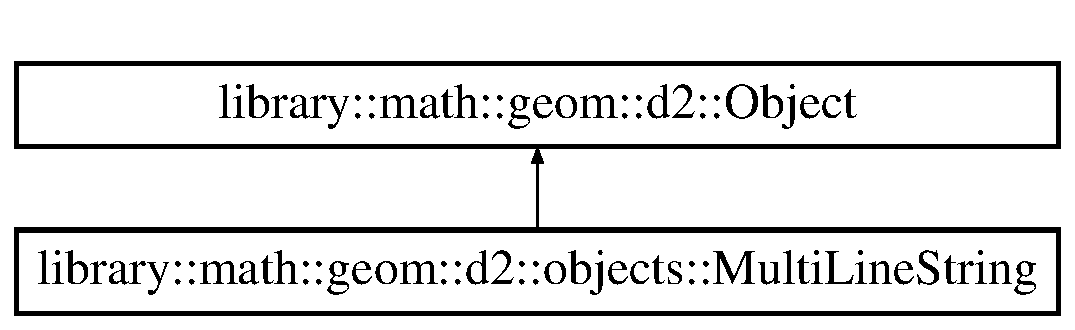
\includegraphics[height=2.000000cm]{classlibrary_1_1math_1_1geom_1_1d2_1_1objects_1_1_multi_line_string}
\end{center}
\end{figure}
\subsection*{Public Types}
\begin{DoxyCompactItemize}
\item 
typedef Array$<$ \hyperlink{classlibrary_1_1math_1_1geom_1_1d2_1_1objects_1_1_line_string}{Line\+String} $>$\+::\hyperlink{classlibrary_1_1math_1_1geom_1_1d2_1_1objects_1_1_multi_line_string_ae9d86dd3f4a78f03347ada9781158b85}{Const\+Iterator} \hyperlink{classlibrary_1_1math_1_1geom_1_1d2_1_1objects_1_1_multi_line_string_ae9d86dd3f4a78f03347ada9781158b85}{Const\+Iterator}
\end{DoxyCompactItemize}
\subsection*{Public Member Functions}
\begin{DoxyCompactItemize}
\item 
\hyperlink{classlibrary_1_1math_1_1geom_1_1d2_1_1objects_1_1_multi_line_string_a8fd6c575f0489484f99c94c607631303}{Multi\+Line\+String} (const Array$<$ \hyperlink{classlibrary_1_1math_1_1geom_1_1d2_1_1objects_1_1_line_string}{Line\+String} $>$ \&a\+Line\+String\+Array)
\begin{DoxyCompactList}\small\item\em Constructor. \end{DoxyCompactList}\item 
virtual \hyperlink{classlibrary_1_1math_1_1geom_1_1d2_1_1objects_1_1_multi_line_string}{Multi\+Line\+String} $\ast$ \hyperlink{classlibrary_1_1math_1_1geom_1_1d2_1_1objects_1_1_multi_line_string_a38054f0f0a2c198b5d3c76ef22562e30}{clone} () const override
\begin{DoxyCompactList}\small\item\em Clone multi line string. \end{DoxyCompactList}\item 
bool \hyperlink{classlibrary_1_1math_1_1geom_1_1d2_1_1objects_1_1_multi_line_string_abc2730ad53ff446aa68f60b28bbfd396}{operator==} (const \hyperlink{classlibrary_1_1math_1_1geom_1_1d2_1_1objects_1_1_multi_line_string}{Multi\+Line\+String} \&a\+Multi\+Line\+String) const
\begin{DoxyCompactList}\small\item\em Equal to operator. \end{DoxyCompactList}\item 
bool \hyperlink{classlibrary_1_1math_1_1geom_1_1d2_1_1objects_1_1_multi_line_string_aa3bde774845839971ad6fd89200fdb76}{operator!=} (const \hyperlink{classlibrary_1_1math_1_1geom_1_1d2_1_1objects_1_1_multi_line_string}{Multi\+Line\+String} \&a\+Multi\+Line\+String) const
\begin{DoxyCompactList}\small\item\em Not equal to operator. \end{DoxyCompactList}\item 
virtual bool \hyperlink{classlibrary_1_1math_1_1geom_1_1d2_1_1objects_1_1_multi_line_string_a77de687b2c287226984e2614dafe744a}{is\+Defined} () const override
\begin{DoxyCompactList}\small\item\em Check if multi multi line string is defined. \end{DoxyCompactList}\item 
bool \hyperlink{classlibrary_1_1math_1_1geom_1_1d2_1_1objects_1_1_multi_line_string_a41b9e07b94cdbe7c2cc9fc49ce8f2d10}{is\+Empty} () const
\begin{DoxyCompactList}\small\item\em Check if multi multi line string is empty. \end{DoxyCompactList}\item 
Size \hyperlink{classlibrary_1_1math_1_1geom_1_1d2_1_1objects_1_1_multi_line_string_a6a4fcd97083f22c5fe163acc0ce23330}{get\+Line\+String\+Count} () const
\begin{DoxyCompactList}\small\item\em Get multi line string count. \end{DoxyCompactList}\item 
Size \hyperlink{classlibrary_1_1math_1_1geom_1_1d2_1_1objects_1_1_multi_line_string_a8d70884126d16f15279c1c16291f5109}{get\+Point\+Count} () const
\begin{DoxyCompactList}\small\item\em Get point count. \end{DoxyCompactList}\item 
\hyperlink{classlibrary_1_1math_1_1geom_1_1d2_1_1objects_1_1_point}{Point} \hyperlink{classlibrary_1_1math_1_1geom_1_1d2_1_1objects_1_1_multi_line_string_ad81881c98cd26ae78544742de4f7be56}{get\+Point\+Closest\+To} (const \hyperlink{classlibrary_1_1math_1_1geom_1_1d2_1_1objects_1_1_point}{Point} \&a\+Point) const
\begin{DoxyCompactList}\small\item\em Get point closest to another point. \end{DoxyCompactList}\item 
virtual String \hyperlink{classlibrary_1_1math_1_1geom_1_1d2_1_1objects_1_1_multi_line_string_a71d1e434196bb8d67054ad28d8aa59a6}{to\+String} (const \hyperlink{classlibrary_1_1math_1_1geom_1_1d2_1_1_object_ac8cd61dada4960cfee9a469231621b17}{Object\+::\+Format} \&a\+Format=\hyperlink{classlibrary_1_1math_1_1geom_1_1d2_1_1_object_ac8cd61dada4960cfee9a469231621b17aeb6d8ae6f20283755b339c0dc273988b}{Object\+::\+Format\+::\+Standard}, const Integer \&a\+Precision=Integer\+::\+Undefined()) const override
\begin{DoxyCompactList}\small\item\em Get string representation. \end{DoxyCompactList}\item 
virtual void \hyperlink{classlibrary_1_1math_1_1geom_1_1d2_1_1objects_1_1_multi_line_string_ab7854c1006501bf5159b890a662198b1}{print} (std\+::ostream \&an\+Output\+Stream, bool display\+Decorators=true) const override
\begin{DoxyCompactList}\small\item\em Print point. \end{DoxyCompactList}\item 
\hyperlink{classlibrary_1_1math_1_1geom_1_1d2_1_1objects_1_1_multi_line_string_ae9d86dd3f4a78f03347ada9781158b85}{Multi\+Line\+String\+::\+Const\+Iterator} \hyperlink{classlibrary_1_1math_1_1geom_1_1d2_1_1objects_1_1_multi_line_string_a4fe1cbb1f12f2ea9f84189db37e6d0c6}{begin} () const
\begin{DoxyCompactList}\small\item\em Get begin const iterator. \end{DoxyCompactList}\item 
\hyperlink{classlibrary_1_1math_1_1geom_1_1d2_1_1objects_1_1_multi_line_string_ae9d86dd3f4a78f03347ada9781158b85}{Multi\+Line\+String\+::\+Const\+Iterator} \hyperlink{classlibrary_1_1math_1_1geom_1_1d2_1_1objects_1_1_multi_line_string_a38c15891b74932039b859b8978eb7b90}{end} () const
\begin{DoxyCompactList}\small\item\em Get end const iterator. \end{DoxyCompactList}\item 
virtual void \hyperlink{classlibrary_1_1math_1_1geom_1_1d2_1_1objects_1_1_multi_line_string_a6180a8b94ff175d6313a74ad4e680bc7}{apply\+Transformation} (const \hyperlink{classlibrary_1_1math_1_1geom_1_1d2_1_1_transformation}{Transformation} \&a\+Transformation) override
\begin{DoxyCompactList}\small\item\em Apply transformation to multi line string. \end{DoxyCompactList}\end{DoxyCompactItemize}
\subsection*{Static Public Member Functions}
\begin{DoxyCompactItemize}
\item 
static \hyperlink{classlibrary_1_1math_1_1geom_1_1d2_1_1objects_1_1_multi_line_string}{Multi\+Line\+String} \hyperlink{classlibrary_1_1math_1_1geom_1_1d2_1_1objects_1_1_multi_line_string_aaa30610df3584b30f80e33ff0f5cd8bb}{Empty} ()
\begin{DoxyCompactList}\small\item\em Constructs an empty multi line string. \end{DoxyCompactList}\end{DoxyCompactItemize}


\subsection{Detailed Description}
Multi Line string. 

\subsection{Member Typedef Documentation}
\mbox{\Hypertarget{classlibrary_1_1math_1_1geom_1_1d2_1_1objects_1_1_multi_line_string_ae9d86dd3f4a78f03347ada9781158b85}\label{classlibrary_1_1math_1_1geom_1_1d2_1_1objects_1_1_multi_line_string_ae9d86dd3f4a78f03347ada9781158b85}} 
\index{library\+::math\+::geom\+::d2\+::objects\+::\+Multi\+Line\+String@{library\+::math\+::geom\+::d2\+::objects\+::\+Multi\+Line\+String}!Const\+Iterator@{Const\+Iterator}}
\index{Const\+Iterator@{Const\+Iterator}!library\+::math\+::geom\+::d2\+::objects\+::\+Multi\+Line\+String@{library\+::math\+::geom\+::d2\+::objects\+::\+Multi\+Line\+String}}
\subsubsection{\texorpdfstring{Const\+Iterator}{ConstIterator}}
{\footnotesize\ttfamily typedef Array$<$\hyperlink{classlibrary_1_1math_1_1geom_1_1d2_1_1objects_1_1_line_string}{Line\+String}$>$\+::\hyperlink{classlibrary_1_1math_1_1geom_1_1d2_1_1objects_1_1_multi_line_string_ae9d86dd3f4a78f03347ada9781158b85}{Const\+Iterator} \hyperlink{classlibrary_1_1math_1_1geom_1_1d2_1_1objects_1_1_multi_line_string_ae9d86dd3f4a78f03347ada9781158b85}{library\+::math\+::geom\+::d2\+::objects\+::\+Multi\+Line\+String\+::\+Const\+Iterator}}



\subsection{Constructor \& Destructor Documentation}
\mbox{\Hypertarget{classlibrary_1_1math_1_1geom_1_1d2_1_1objects_1_1_multi_line_string_a8fd6c575f0489484f99c94c607631303}\label{classlibrary_1_1math_1_1geom_1_1d2_1_1objects_1_1_multi_line_string_a8fd6c575f0489484f99c94c607631303}} 
\index{library\+::math\+::geom\+::d2\+::objects\+::\+Multi\+Line\+String@{library\+::math\+::geom\+::d2\+::objects\+::\+Multi\+Line\+String}!Multi\+Line\+String@{Multi\+Line\+String}}
\index{Multi\+Line\+String@{Multi\+Line\+String}!library\+::math\+::geom\+::d2\+::objects\+::\+Multi\+Line\+String@{library\+::math\+::geom\+::d2\+::objects\+::\+Multi\+Line\+String}}
\subsubsection{\texorpdfstring{Multi\+Line\+String()}{MultiLineString()}}
{\footnotesize\ttfamily library\+::math\+::geom\+::d2\+::objects\+::\+Multi\+Line\+String\+::\+Multi\+Line\+String (\begin{DoxyParamCaption}\item[{const Array$<$ \hyperlink{classlibrary_1_1math_1_1geom_1_1d2_1_1objects_1_1_line_string}{Line\+String} $>$ \&}]{a\+Line\+String\+Array }\end{DoxyParamCaption})}



Constructor. 


\begin{DoxyCode}
\hyperlink{classlibrary_1_1math_1_1geom_1_1d2_1_1objects_1_1_multi_line_string_a8fd6c575f0489484f99c94c607631303}{MultiLineString} multiLineString(\{ \{ 0.0, 0.0 \}, \{ 0.0, 1.0 \}, \{ 1.0, 0.0 \} \}) ;
\end{DoxyCode}



\begin{DoxyParams}[1]{Parameters}
\mbox{\tt in}  & {\em a\+Point\+Array} & A point array \\
\hline
\end{DoxyParams}


\subsection{Member Function Documentation}
\mbox{\Hypertarget{classlibrary_1_1math_1_1geom_1_1d2_1_1objects_1_1_multi_line_string_a6180a8b94ff175d6313a74ad4e680bc7}\label{classlibrary_1_1math_1_1geom_1_1d2_1_1objects_1_1_multi_line_string_a6180a8b94ff175d6313a74ad4e680bc7}} 
\index{library\+::math\+::geom\+::d2\+::objects\+::\+Multi\+Line\+String@{library\+::math\+::geom\+::d2\+::objects\+::\+Multi\+Line\+String}!apply\+Transformation@{apply\+Transformation}}
\index{apply\+Transformation@{apply\+Transformation}!library\+::math\+::geom\+::d2\+::objects\+::\+Multi\+Line\+String@{library\+::math\+::geom\+::d2\+::objects\+::\+Multi\+Line\+String}}
\subsubsection{\texorpdfstring{apply\+Transformation()}{applyTransformation()}}
{\footnotesize\ttfamily virtual void library\+::math\+::geom\+::d2\+::objects\+::\+Multi\+Line\+String\+::apply\+Transformation (\begin{DoxyParamCaption}\item[{const \hyperlink{classlibrary_1_1math_1_1geom_1_1d2_1_1_transformation}{Transformation} \&}]{a\+Transformation }\end{DoxyParamCaption})\hspace{0.3cm}{\ttfamily [override]}, {\ttfamily [virtual]}}



Apply transformation to multi line string. 


\begin{DoxyParams}[1]{Parameters}
\mbox{\tt in}  & {\em a\+Transformation} & A transformation \\
\hline
\end{DoxyParams}


Implements \hyperlink{classlibrary_1_1math_1_1geom_1_1d2_1_1_object_a289589fb6e9e7a2c4ca4976a1544def5}{library\+::math\+::geom\+::d2\+::\+Object}.

\mbox{\Hypertarget{classlibrary_1_1math_1_1geom_1_1d2_1_1objects_1_1_multi_line_string_a4fe1cbb1f12f2ea9f84189db37e6d0c6}\label{classlibrary_1_1math_1_1geom_1_1d2_1_1objects_1_1_multi_line_string_a4fe1cbb1f12f2ea9f84189db37e6d0c6}} 
\index{library\+::math\+::geom\+::d2\+::objects\+::\+Multi\+Line\+String@{library\+::math\+::geom\+::d2\+::objects\+::\+Multi\+Line\+String}!begin@{begin}}
\index{begin@{begin}!library\+::math\+::geom\+::d2\+::objects\+::\+Multi\+Line\+String@{library\+::math\+::geom\+::d2\+::objects\+::\+Multi\+Line\+String}}
\subsubsection{\texorpdfstring{begin()}{begin()}}
{\footnotesize\ttfamily \hyperlink{classlibrary_1_1math_1_1geom_1_1d2_1_1objects_1_1_multi_line_string_ae9d86dd3f4a78f03347ada9781158b85}{Multi\+Line\+String\+::\+Const\+Iterator} library\+::math\+::geom\+::d2\+::objects\+::\+Multi\+Line\+String\+::begin (\begin{DoxyParamCaption}{ }\end{DoxyParamCaption}) const}



Get begin const iterator. 

\begin{DoxyReturn}{Returns}
Begin const iterator 
\end{DoxyReturn}
\mbox{\Hypertarget{classlibrary_1_1math_1_1geom_1_1d2_1_1objects_1_1_multi_line_string_a38054f0f0a2c198b5d3c76ef22562e30}\label{classlibrary_1_1math_1_1geom_1_1d2_1_1objects_1_1_multi_line_string_a38054f0f0a2c198b5d3c76ef22562e30}} 
\index{library\+::math\+::geom\+::d2\+::objects\+::\+Multi\+Line\+String@{library\+::math\+::geom\+::d2\+::objects\+::\+Multi\+Line\+String}!clone@{clone}}
\index{clone@{clone}!library\+::math\+::geom\+::d2\+::objects\+::\+Multi\+Line\+String@{library\+::math\+::geom\+::d2\+::objects\+::\+Multi\+Line\+String}}
\subsubsection{\texorpdfstring{clone()}{clone()}}
{\footnotesize\ttfamily virtual \hyperlink{classlibrary_1_1math_1_1geom_1_1d2_1_1objects_1_1_multi_line_string}{Multi\+Line\+String}$\ast$ library\+::math\+::geom\+::d2\+::objects\+::\+Multi\+Line\+String\+::clone (\begin{DoxyParamCaption}{ }\end{DoxyParamCaption}) const\hspace{0.3cm}{\ttfamily [override]}, {\ttfamily [virtual]}}



Clone multi line string. 

\begin{DoxyReturn}{Returns}
Pointer to cloned multi line string 
\end{DoxyReturn}


Implements \hyperlink{classlibrary_1_1math_1_1geom_1_1d2_1_1_object_a5c26ae4120edb24f6463d65a9cef247d}{library\+::math\+::geom\+::d2\+::\+Object}.

\mbox{\Hypertarget{classlibrary_1_1math_1_1geom_1_1d2_1_1objects_1_1_multi_line_string_aaa30610df3584b30f80e33ff0f5cd8bb}\label{classlibrary_1_1math_1_1geom_1_1d2_1_1objects_1_1_multi_line_string_aaa30610df3584b30f80e33ff0f5cd8bb}} 
\index{library\+::math\+::geom\+::d2\+::objects\+::\+Multi\+Line\+String@{library\+::math\+::geom\+::d2\+::objects\+::\+Multi\+Line\+String}!Empty@{Empty}}
\index{Empty@{Empty}!library\+::math\+::geom\+::d2\+::objects\+::\+Multi\+Line\+String@{library\+::math\+::geom\+::d2\+::objects\+::\+Multi\+Line\+String}}
\subsubsection{\texorpdfstring{Empty()}{Empty()}}
{\footnotesize\ttfamily static \hyperlink{classlibrary_1_1math_1_1geom_1_1d2_1_1objects_1_1_multi_line_string}{Multi\+Line\+String} library\+::math\+::geom\+::d2\+::objects\+::\+Multi\+Line\+String\+::\+Empty (\begin{DoxyParamCaption}{ }\end{DoxyParamCaption})\hspace{0.3cm}{\ttfamily [static]}}



Constructs an empty multi line string. 


\begin{DoxyCode}
\hyperlink{classlibrary_1_1math_1_1geom_1_1d2_1_1objects_1_1_multi_line_string_a8fd6c575f0489484f99c94c607631303}{MultiLineString} multiLineString = \hyperlink{classlibrary_1_1math_1_1geom_1_1d2_1_1objects_1_1_multi_line_string_aaa30610df3584b30f80e33ff0f5cd8bb}{MultiLineString::Empty}() ;
\end{DoxyCode}


\begin{DoxyReturn}{Returns}
Empty multi line string 
\end{DoxyReturn}
\mbox{\Hypertarget{classlibrary_1_1math_1_1geom_1_1d2_1_1objects_1_1_multi_line_string_a38c15891b74932039b859b8978eb7b90}\label{classlibrary_1_1math_1_1geom_1_1d2_1_1objects_1_1_multi_line_string_a38c15891b74932039b859b8978eb7b90}} 
\index{library\+::math\+::geom\+::d2\+::objects\+::\+Multi\+Line\+String@{library\+::math\+::geom\+::d2\+::objects\+::\+Multi\+Line\+String}!end@{end}}
\index{end@{end}!library\+::math\+::geom\+::d2\+::objects\+::\+Multi\+Line\+String@{library\+::math\+::geom\+::d2\+::objects\+::\+Multi\+Line\+String}}
\subsubsection{\texorpdfstring{end()}{end()}}
{\footnotesize\ttfamily \hyperlink{classlibrary_1_1math_1_1geom_1_1d2_1_1objects_1_1_multi_line_string_ae9d86dd3f4a78f03347ada9781158b85}{Multi\+Line\+String\+::\+Const\+Iterator} library\+::math\+::geom\+::d2\+::objects\+::\+Multi\+Line\+String\+::end (\begin{DoxyParamCaption}{ }\end{DoxyParamCaption}) const}



Get end const iterator. 

\begin{DoxyReturn}{Returns}
End const iterator 
\end{DoxyReturn}
\mbox{\Hypertarget{classlibrary_1_1math_1_1geom_1_1d2_1_1objects_1_1_multi_line_string_a6a4fcd97083f22c5fe163acc0ce23330}\label{classlibrary_1_1math_1_1geom_1_1d2_1_1objects_1_1_multi_line_string_a6a4fcd97083f22c5fe163acc0ce23330}} 
\index{library\+::math\+::geom\+::d2\+::objects\+::\+Multi\+Line\+String@{library\+::math\+::geom\+::d2\+::objects\+::\+Multi\+Line\+String}!get\+Line\+String\+Count@{get\+Line\+String\+Count}}
\index{get\+Line\+String\+Count@{get\+Line\+String\+Count}!library\+::math\+::geom\+::d2\+::objects\+::\+Multi\+Line\+String@{library\+::math\+::geom\+::d2\+::objects\+::\+Multi\+Line\+String}}
\subsubsection{\texorpdfstring{get\+Line\+String\+Count()}{getLineStringCount()}}
{\footnotesize\ttfamily Size library\+::math\+::geom\+::d2\+::objects\+::\+Multi\+Line\+String\+::get\+Line\+String\+Count (\begin{DoxyParamCaption}{ }\end{DoxyParamCaption}) const}



Get multi line string count. 

\begin{DoxyReturn}{Returns}
multi Line string count 
\end{DoxyReturn}
\mbox{\Hypertarget{classlibrary_1_1math_1_1geom_1_1d2_1_1objects_1_1_multi_line_string_ad81881c98cd26ae78544742de4f7be56}\label{classlibrary_1_1math_1_1geom_1_1d2_1_1objects_1_1_multi_line_string_ad81881c98cd26ae78544742de4f7be56}} 
\index{library\+::math\+::geom\+::d2\+::objects\+::\+Multi\+Line\+String@{library\+::math\+::geom\+::d2\+::objects\+::\+Multi\+Line\+String}!get\+Point\+Closest\+To@{get\+Point\+Closest\+To}}
\index{get\+Point\+Closest\+To@{get\+Point\+Closest\+To}!library\+::math\+::geom\+::d2\+::objects\+::\+Multi\+Line\+String@{library\+::math\+::geom\+::d2\+::objects\+::\+Multi\+Line\+String}}
\subsubsection{\texorpdfstring{get\+Point\+Closest\+To()}{getPointClosestTo()}}
{\footnotesize\ttfamily \hyperlink{classlibrary_1_1math_1_1geom_1_1d2_1_1objects_1_1_point}{Point} library\+::math\+::geom\+::d2\+::objects\+::\+Multi\+Line\+String\+::get\+Point\+Closest\+To (\begin{DoxyParamCaption}\item[{const \hyperlink{classlibrary_1_1math_1_1geom_1_1d2_1_1objects_1_1_point}{Point} \&}]{a\+Point }\end{DoxyParamCaption}) const}



Get point closest to another point. 


\begin{DoxyParams}[1]{Parameters}
\mbox{\tt in}  & {\em a\+Point} & A point \\
\hline
\end{DoxyParams}
\begin{DoxyReturn}{Returns}
Closest point 
\end{DoxyReturn}
\mbox{\Hypertarget{classlibrary_1_1math_1_1geom_1_1d2_1_1objects_1_1_multi_line_string_a8d70884126d16f15279c1c16291f5109}\label{classlibrary_1_1math_1_1geom_1_1d2_1_1objects_1_1_multi_line_string_a8d70884126d16f15279c1c16291f5109}} 
\index{library\+::math\+::geom\+::d2\+::objects\+::\+Multi\+Line\+String@{library\+::math\+::geom\+::d2\+::objects\+::\+Multi\+Line\+String}!get\+Point\+Count@{get\+Point\+Count}}
\index{get\+Point\+Count@{get\+Point\+Count}!library\+::math\+::geom\+::d2\+::objects\+::\+Multi\+Line\+String@{library\+::math\+::geom\+::d2\+::objects\+::\+Multi\+Line\+String}}
\subsubsection{\texorpdfstring{get\+Point\+Count()}{getPointCount()}}
{\footnotesize\ttfamily Size library\+::math\+::geom\+::d2\+::objects\+::\+Multi\+Line\+String\+::get\+Point\+Count (\begin{DoxyParamCaption}{ }\end{DoxyParamCaption}) const}



Get point count. 

\begin{DoxyReturn}{Returns}
\hyperlink{classlibrary_1_1math_1_1geom_1_1d2_1_1objects_1_1_point}{Point} count 
\end{DoxyReturn}
\mbox{\Hypertarget{classlibrary_1_1math_1_1geom_1_1d2_1_1objects_1_1_multi_line_string_a77de687b2c287226984e2614dafe744a}\label{classlibrary_1_1math_1_1geom_1_1d2_1_1objects_1_1_multi_line_string_a77de687b2c287226984e2614dafe744a}} 
\index{library\+::math\+::geom\+::d2\+::objects\+::\+Multi\+Line\+String@{library\+::math\+::geom\+::d2\+::objects\+::\+Multi\+Line\+String}!is\+Defined@{is\+Defined}}
\index{is\+Defined@{is\+Defined}!library\+::math\+::geom\+::d2\+::objects\+::\+Multi\+Line\+String@{library\+::math\+::geom\+::d2\+::objects\+::\+Multi\+Line\+String}}
\subsubsection{\texorpdfstring{is\+Defined()}{isDefined()}}
{\footnotesize\ttfamily virtual bool library\+::math\+::geom\+::d2\+::objects\+::\+Multi\+Line\+String\+::is\+Defined (\begin{DoxyParamCaption}{ }\end{DoxyParamCaption}) const\hspace{0.3cm}{\ttfamily [override]}, {\ttfamily [virtual]}}



Check if multi multi line string is defined. 


\begin{DoxyCode}
\hyperlink{classlibrary_1_1math_1_1geom_1_1d2_1_1objects_1_1_multi_line_string_a8fd6c575f0489484f99c94c607631303}{MultiLineString}(0.0, 0.0).isDefined() ; \textcolor{comment}{// True}
\end{DoxyCode}


\begin{DoxyReturn}{Returns}
True if multi multi line string is defined 
\end{DoxyReturn}


Implements \hyperlink{classlibrary_1_1math_1_1geom_1_1d2_1_1_object_ae9506254971168a3ca63e1923556b70d}{library\+::math\+::geom\+::d2\+::\+Object}.

\mbox{\Hypertarget{classlibrary_1_1math_1_1geom_1_1d2_1_1objects_1_1_multi_line_string_a41b9e07b94cdbe7c2cc9fc49ce8f2d10}\label{classlibrary_1_1math_1_1geom_1_1d2_1_1objects_1_1_multi_line_string_a41b9e07b94cdbe7c2cc9fc49ce8f2d10}} 
\index{library\+::math\+::geom\+::d2\+::objects\+::\+Multi\+Line\+String@{library\+::math\+::geom\+::d2\+::objects\+::\+Multi\+Line\+String}!is\+Empty@{is\+Empty}}
\index{is\+Empty@{is\+Empty}!library\+::math\+::geom\+::d2\+::objects\+::\+Multi\+Line\+String@{library\+::math\+::geom\+::d2\+::objects\+::\+Multi\+Line\+String}}
\subsubsection{\texorpdfstring{is\+Empty()}{isEmpty()}}
{\footnotesize\ttfamily bool library\+::math\+::geom\+::d2\+::objects\+::\+Multi\+Line\+String\+::is\+Empty (\begin{DoxyParamCaption}{ }\end{DoxyParamCaption}) const}



Check if multi multi line string is empty. 


\begin{DoxyCode}
\hyperlink{classlibrary_1_1math_1_1geom_1_1d2_1_1objects_1_1_multi_line_string_aaa30610df3584b30f80e33ff0f5cd8bb}{MultiLineString::Empty}().\hyperlink{classlibrary_1_1math_1_1geom_1_1d2_1_1objects_1_1_multi_line_string_a41b9e07b94cdbe7c2cc9fc49ce8f2d10}{isEmpty}() ; \textcolor{comment}{// True}
\end{DoxyCode}


\begin{DoxyReturn}{Returns}
True if multi multi line string is empty 
\end{DoxyReturn}
\mbox{\Hypertarget{classlibrary_1_1math_1_1geom_1_1d2_1_1objects_1_1_multi_line_string_aa3bde774845839971ad6fd89200fdb76}\label{classlibrary_1_1math_1_1geom_1_1d2_1_1objects_1_1_multi_line_string_aa3bde774845839971ad6fd89200fdb76}} 
\index{library\+::math\+::geom\+::d2\+::objects\+::\+Multi\+Line\+String@{library\+::math\+::geom\+::d2\+::objects\+::\+Multi\+Line\+String}!operator"!=@{operator"!=}}
\index{operator"!=@{operator"!=}!library\+::math\+::geom\+::d2\+::objects\+::\+Multi\+Line\+String@{library\+::math\+::geom\+::d2\+::objects\+::\+Multi\+Line\+String}}
\subsubsection{\texorpdfstring{operator"!=()}{operator!=()}}
{\footnotesize\ttfamily bool library\+::math\+::geom\+::d2\+::objects\+::\+Multi\+Line\+String\+::operator!= (\begin{DoxyParamCaption}\item[{const \hyperlink{classlibrary_1_1math_1_1geom_1_1d2_1_1objects_1_1_multi_line_string}{Multi\+Line\+String} \&}]{a\+Multi\+Line\+String }\end{DoxyParamCaption}) const}



Not equal to operator. 


\begin{DoxyParams}[1]{Parameters}
\mbox{\tt in}  & {\em a\+Multi\+Line\+String} & A multi multi line string \\
\hline
\end{DoxyParams}
\begin{DoxyReturn}{Returns}
True if multi multi line strings are not equal 
\end{DoxyReturn}
\mbox{\Hypertarget{classlibrary_1_1math_1_1geom_1_1d2_1_1objects_1_1_multi_line_string_abc2730ad53ff446aa68f60b28bbfd396}\label{classlibrary_1_1math_1_1geom_1_1d2_1_1objects_1_1_multi_line_string_abc2730ad53ff446aa68f60b28bbfd396}} 
\index{library\+::math\+::geom\+::d2\+::objects\+::\+Multi\+Line\+String@{library\+::math\+::geom\+::d2\+::objects\+::\+Multi\+Line\+String}!operator==@{operator==}}
\index{operator==@{operator==}!library\+::math\+::geom\+::d2\+::objects\+::\+Multi\+Line\+String@{library\+::math\+::geom\+::d2\+::objects\+::\+Multi\+Line\+String}}
\subsubsection{\texorpdfstring{operator==()}{operator==()}}
{\footnotesize\ttfamily bool library\+::math\+::geom\+::d2\+::objects\+::\+Multi\+Line\+String\+::operator== (\begin{DoxyParamCaption}\item[{const \hyperlink{classlibrary_1_1math_1_1geom_1_1d2_1_1objects_1_1_multi_line_string}{Multi\+Line\+String} \&}]{a\+Multi\+Line\+String }\end{DoxyParamCaption}) const}



Equal to operator. 


\begin{DoxyParams}[1]{Parameters}
\mbox{\tt in}  & {\em a\+Multi\+Line\+String} & A multi multi line string \\
\hline
\end{DoxyParams}
\begin{DoxyReturn}{Returns}
True if multi multi line strings are equal 
\end{DoxyReturn}
\mbox{\Hypertarget{classlibrary_1_1math_1_1geom_1_1d2_1_1objects_1_1_multi_line_string_ab7854c1006501bf5159b890a662198b1}\label{classlibrary_1_1math_1_1geom_1_1d2_1_1objects_1_1_multi_line_string_ab7854c1006501bf5159b890a662198b1}} 
\index{library\+::math\+::geom\+::d2\+::objects\+::\+Multi\+Line\+String@{library\+::math\+::geom\+::d2\+::objects\+::\+Multi\+Line\+String}!print@{print}}
\index{print@{print}!library\+::math\+::geom\+::d2\+::objects\+::\+Multi\+Line\+String@{library\+::math\+::geom\+::d2\+::objects\+::\+Multi\+Line\+String}}
\subsubsection{\texorpdfstring{print()}{print()}}
{\footnotesize\ttfamily virtual void library\+::math\+::geom\+::d2\+::objects\+::\+Multi\+Line\+String\+::print (\begin{DoxyParamCaption}\item[{std\+::ostream \&}]{an\+Output\+Stream,  }\item[{bool}]{display\+Decorators = {\ttfamily true} }\end{DoxyParamCaption}) const\hspace{0.3cm}{\ttfamily [override]}, {\ttfamily [virtual]}}



Print point. 


\begin{DoxyParams}[1]{Parameters}
\mbox{\tt in}  & {\em an\+Output\+Stream} & An output stream \\
\hline
\mbox{\tt in}  & {\em (optional)} & display\+Decorators If true, display decorators \\
\hline
\end{DoxyParams}


Implements \hyperlink{classlibrary_1_1math_1_1geom_1_1d2_1_1_object_a834bbf59cf1c483d1dc7b0966b1e1ab3}{library\+::math\+::geom\+::d2\+::\+Object}.

\mbox{\Hypertarget{classlibrary_1_1math_1_1geom_1_1d2_1_1objects_1_1_multi_line_string_a71d1e434196bb8d67054ad28d8aa59a6}\label{classlibrary_1_1math_1_1geom_1_1d2_1_1objects_1_1_multi_line_string_a71d1e434196bb8d67054ad28d8aa59a6}} 
\index{library\+::math\+::geom\+::d2\+::objects\+::\+Multi\+Line\+String@{library\+::math\+::geom\+::d2\+::objects\+::\+Multi\+Line\+String}!to\+String@{to\+String}}
\index{to\+String@{to\+String}!library\+::math\+::geom\+::d2\+::objects\+::\+Multi\+Line\+String@{library\+::math\+::geom\+::d2\+::objects\+::\+Multi\+Line\+String}}
\subsubsection{\texorpdfstring{to\+String()}{toString()}}
{\footnotesize\ttfamily virtual String library\+::math\+::geom\+::d2\+::objects\+::\+Multi\+Line\+String\+::to\+String (\begin{DoxyParamCaption}\item[{const \hyperlink{classlibrary_1_1math_1_1geom_1_1d2_1_1_object_ac8cd61dada4960cfee9a469231621b17}{Object\+::\+Format} \&}]{a\+Format = {\ttfamily \hyperlink{classlibrary_1_1math_1_1geom_1_1d2_1_1_object_ac8cd61dada4960cfee9a469231621b17aeb6d8ae6f20283755b339c0dc273988b}{Object\+::\+Format\+::\+Standard}},  }\item[{const Integer \&}]{a\+Precision = {\ttfamily Integer\+:\+:Undefined()} }\end{DoxyParamCaption}) const\hspace{0.3cm}{\ttfamily [override]}, {\ttfamily [virtual]}}



Get string representation. 


\begin{DoxyParams}[1]{Parameters}
\mbox{\tt in}  & {\em a\+Format} & A format \\
\hline
\end{DoxyParams}
\begin{DoxyReturn}{Returns}
String representation 
\end{DoxyReturn}


Implements \hyperlink{classlibrary_1_1math_1_1geom_1_1d2_1_1_object_acdd76b3637732a249536b609dbe3f0eb}{library\+::math\+::geom\+::d2\+::\+Object}.



The documentation for this class was generated from the following file\+:\begin{DoxyCompactItemize}
\item 
include/\+Library/\+Mathematics/\+Geometry/2\+D/\+Objects/\hyperlink{_multi_line_string_8hpp}{Multi\+Line\+String.\+hpp}\end{DoxyCompactItemize}

\hypertarget{classlibrary_1_1math_1_1geom_1_1d2_1_1objects_1_1_multi_polygon}{}\section{library\+:\+:math\+:\+:geom\+:\+:d2\+:\+:objects\+:\+:Multi\+Polygon Class Reference}
\label{classlibrary_1_1math_1_1geom_1_1d2_1_1objects_1_1_multi_polygon}\index{library\+::math\+::geom\+::d2\+::objects\+::\+Multi\+Polygon@{library\+::math\+::geom\+::d2\+::objects\+::\+Multi\+Polygon}}


Multi-\/polygon.  




{\ttfamily \#include $<$Multi\+Polygon.\+hpp$>$}

Inheritance diagram for library\+:\+:math\+:\+:geom\+:\+:d2\+:\+:objects\+:\+:Multi\+Polygon\+:\begin{figure}[H]
\begin{center}
\leavevmode
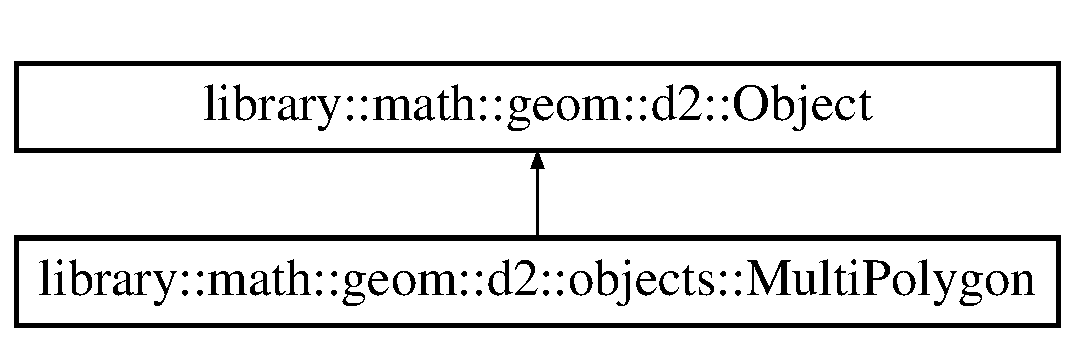
\includegraphics[height=2.000000cm]{classlibrary_1_1math_1_1geom_1_1d2_1_1objects_1_1_multi_polygon}
\end{center}
\end{figure}
\subsection*{Public Member Functions}
\begin{DoxyCompactItemize}
\item 
\hyperlink{classlibrary_1_1math_1_1geom_1_1d2_1_1objects_1_1_multi_polygon_a10c2390027c64a8541efde7fcb2b282f}{Multi\+Polygon} (const Array$<$ \hyperlink{classlibrary_1_1math_1_1geom_1_1d2_1_1objects_1_1_polygon}{Polygon} $>$ \&a\+Polygon\+Array=Array$<$ \hyperlink{classlibrary_1_1math_1_1geom_1_1d2_1_1objects_1_1_polygon}{Polygon} $>$\+::Empty())
\begin{DoxyCompactList}\small\item\em Constructor. \end{DoxyCompactList}\item 
\hyperlink{classlibrary_1_1math_1_1geom_1_1d2_1_1objects_1_1_multi_polygon_a2a64713865d9b308dbfcb56c209fdf56}{Multi\+Polygon} (const \hyperlink{classlibrary_1_1math_1_1geom_1_1d2_1_1objects_1_1_multi_polygon}{Multi\+Polygon} \&a\+Multi\+Polygon)
\begin{DoxyCompactList}\small\item\em Copy constructor. \end{DoxyCompactList}\item 
virtual \hyperlink{classlibrary_1_1math_1_1geom_1_1d2_1_1objects_1_1_multi_polygon_a4aa98e616ff0085fc1390bca368c984c}{$\sim$\+Multi\+Polygon} () override
\begin{DoxyCompactList}\small\item\em Destructor (virtual) \end{DoxyCompactList}\item 
\hyperlink{classlibrary_1_1math_1_1geom_1_1d2_1_1objects_1_1_multi_polygon}{Multi\+Polygon} \& \hyperlink{classlibrary_1_1math_1_1geom_1_1d2_1_1objects_1_1_multi_polygon_abd2fa0b95f3b339dda6e4b8ccd321af0}{operator=} (const \hyperlink{classlibrary_1_1math_1_1geom_1_1d2_1_1objects_1_1_multi_polygon}{Multi\+Polygon} \&a\+Multi\+Polygon)
\begin{DoxyCompactList}\small\item\em Copy assignment operator. \end{DoxyCompactList}\item 
virtual \hyperlink{classlibrary_1_1math_1_1geom_1_1d2_1_1objects_1_1_multi_polygon}{Multi\+Polygon} $\ast$ \hyperlink{classlibrary_1_1math_1_1geom_1_1d2_1_1objects_1_1_multi_polygon_a6dc8db614de9fb615491deb783fe7fcd}{clone} () const override
\begin{DoxyCompactList}\small\item\em Clone multi-\/polygon. \end{DoxyCompactList}\item 
bool \hyperlink{classlibrary_1_1math_1_1geom_1_1d2_1_1objects_1_1_multi_polygon_a3032f68e33b1bb90cbf021008124bccd}{operator==} (const \hyperlink{classlibrary_1_1math_1_1geom_1_1d2_1_1objects_1_1_multi_polygon}{Multi\+Polygon} \&a\+Multi\+Polygon) const
\begin{DoxyCompactList}\small\item\em Equal to operator. \end{DoxyCompactList}\item 
bool \hyperlink{classlibrary_1_1math_1_1geom_1_1d2_1_1objects_1_1_multi_polygon_a7478631c89b146b6dcd4814a521c0200}{operator!=} (const \hyperlink{classlibrary_1_1math_1_1geom_1_1d2_1_1objects_1_1_multi_polygon}{Multi\+Polygon} \&a\+Multi\+Polygon) const
\begin{DoxyCompactList}\small\item\em Not equal to operator. \end{DoxyCompactList}\item 
virtual bool \hyperlink{classlibrary_1_1math_1_1geom_1_1d2_1_1objects_1_1_multi_polygon_a9afa806e12102255fc5abf8a94106089}{is\+Defined} () const override
\begin{DoxyCompactList}\small\item\em Check if multi-\/polygon is defined. \end{DoxyCompactList}\item 
bool \hyperlink{classlibrary_1_1math_1_1geom_1_1d2_1_1objects_1_1_multi_polygon_a9b11d0b3d9a341f541cebcd032227986}{contains} (const \hyperlink{classlibrary_1_1math_1_1geom_1_1d2_1_1objects_1_1_point}{Point} \&a\+Point) const
\begin{DoxyCompactList}\small\item\em Check if multi-\/polygon contains point. \end{DoxyCompactList}\item 
bool \hyperlink{classlibrary_1_1math_1_1geom_1_1d2_1_1objects_1_1_multi_polygon_a3a123cc4ebd6d157c1774176054617b6}{contains} (const \hyperlink{classlibrary_1_1math_1_1geom_1_1d2_1_1objects_1_1_point_set}{Point\+Set} \&a\+Point\+Set) const
\begin{DoxyCompactList}\small\item\em Check if multi-\/polygon contains point set. \end{DoxyCompactList}\item 
Size \hyperlink{classlibrary_1_1math_1_1geom_1_1d2_1_1objects_1_1_multi_polygon_ac2a7a8791732ddd249a2bee8d476b7ae}{get\+Polygon\+Count} () const
\begin{DoxyCompactList}\small\item\em Get number of polygons. \end{DoxyCompactList}\item 
\hyperlink{classlibrary_1_1math_1_1geom_1_1d2_1_1objects_1_1_multi_polygon}{Multi\+Polygon} \hyperlink{classlibrary_1_1math_1_1geom_1_1d2_1_1objects_1_1_multi_polygon_ad27159b10d8cb05d9ed15f1dd2d3de1d}{union\+With} (const \hyperlink{classlibrary_1_1math_1_1geom_1_1d2_1_1objects_1_1_multi_polygon}{Multi\+Polygon} \&a\+Multi\+Polygon) const
\begin{DoxyCompactList}\small\item\em Compute intersection of multi-\/polygon with multi-\/polygon. \end{DoxyCompactList}\item 
virtual String \hyperlink{classlibrary_1_1math_1_1geom_1_1d2_1_1objects_1_1_multi_polygon_a598e024d69ca9a99d97cf7412b334869}{to\+String} (const \hyperlink{classlibrary_1_1math_1_1geom_1_1d2_1_1_object_ac8cd61dada4960cfee9a469231621b17}{Object\+::\+Format} \&a\+Format=\hyperlink{classlibrary_1_1math_1_1geom_1_1d2_1_1_object_ac8cd61dada4960cfee9a469231621b17aeb6d8ae6f20283755b339c0dc273988b}{Object\+::\+Format\+::\+Standard}, const Integer \&a\+Precision=Integer\+::\+Undefined()) const override
\begin{DoxyCompactList}\small\item\em Get string representation. \end{DoxyCompactList}\item 
virtual void \hyperlink{classlibrary_1_1math_1_1geom_1_1d2_1_1objects_1_1_multi_polygon_aa1998e9d86d24edb61e978f397148d1c}{print} (std\+::ostream \&an\+Output\+Stream, bool display\+Decorators=true) const override
\begin{DoxyCompactList}\small\item\em Print multi-\/polygon. \end{DoxyCompactList}\item 
virtual void \hyperlink{classlibrary_1_1math_1_1geom_1_1d2_1_1objects_1_1_multi_polygon_af4adcde904edd77d54236517652e4da1}{apply\+Transformation} (const \hyperlink{classlibrary_1_1math_1_1geom_1_1d2_1_1_transformation}{Transformation} \&a\+Transformation) override
\begin{DoxyCompactList}\small\item\em Apply transformation to multi-\/polygon. \end{DoxyCompactList}\end{DoxyCompactItemize}
\subsection*{Static Public Member Functions}
\begin{DoxyCompactItemize}
\item 
static \hyperlink{classlibrary_1_1math_1_1geom_1_1d2_1_1objects_1_1_multi_polygon}{Multi\+Polygon} \hyperlink{classlibrary_1_1math_1_1geom_1_1d2_1_1objects_1_1_multi_polygon_a92c7c7ece7479f0ac9a9b75546b69b20}{Undefined} ()
\begin{DoxyCompactList}\small\item\em Constructs an undefined multi-\/polygon. \end{DoxyCompactList}\end{DoxyCompactItemize}
\subsection*{Additional Inherited Members}


\subsection{Detailed Description}
Multi-\/polygon. 

\subsection{Constructor \& Destructor Documentation}
\mbox{\Hypertarget{classlibrary_1_1math_1_1geom_1_1d2_1_1objects_1_1_multi_polygon_a10c2390027c64a8541efde7fcb2b282f}\label{classlibrary_1_1math_1_1geom_1_1d2_1_1objects_1_1_multi_polygon_a10c2390027c64a8541efde7fcb2b282f}} 
\index{library\+::math\+::geom\+::d2\+::objects\+::\+Multi\+Polygon@{library\+::math\+::geom\+::d2\+::objects\+::\+Multi\+Polygon}!Multi\+Polygon@{Multi\+Polygon}}
\index{Multi\+Polygon@{Multi\+Polygon}!library\+::math\+::geom\+::d2\+::objects\+::\+Multi\+Polygon@{library\+::math\+::geom\+::d2\+::objects\+::\+Multi\+Polygon}}
\subsubsection{\texorpdfstring{Multi\+Polygon()}{MultiPolygon()}\hspace{0.1cm}{\footnotesize\ttfamily [1/2]}}
{\footnotesize\ttfamily library\+::math\+::geom\+::d2\+::objects\+::\+Multi\+Polygon\+::\+Multi\+Polygon (\begin{DoxyParamCaption}\item[{const Array$<$ \hyperlink{classlibrary_1_1math_1_1geom_1_1d2_1_1objects_1_1_polygon}{Polygon} $>$ \&}]{a\+Polygon\+Array = {\ttfamily Array$<$\hyperlink{classlibrary_1_1math_1_1geom_1_1d2_1_1objects_1_1_polygon}{Polygon}$>$\+:\+:Empty()} }\end{DoxyParamCaption})}



Constructor. 


\begin{DoxyParams}[1]{Parameters}
\mbox{\tt in}  & {\em a\+Polygon\+Array} & An array of polygons \\
\hline
\end{DoxyParams}
\mbox{\Hypertarget{classlibrary_1_1math_1_1geom_1_1d2_1_1objects_1_1_multi_polygon_a2a64713865d9b308dbfcb56c209fdf56}\label{classlibrary_1_1math_1_1geom_1_1d2_1_1objects_1_1_multi_polygon_a2a64713865d9b308dbfcb56c209fdf56}} 
\index{library\+::math\+::geom\+::d2\+::objects\+::\+Multi\+Polygon@{library\+::math\+::geom\+::d2\+::objects\+::\+Multi\+Polygon}!Multi\+Polygon@{Multi\+Polygon}}
\index{Multi\+Polygon@{Multi\+Polygon}!library\+::math\+::geom\+::d2\+::objects\+::\+Multi\+Polygon@{library\+::math\+::geom\+::d2\+::objects\+::\+Multi\+Polygon}}
\subsubsection{\texorpdfstring{Multi\+Polygon()}{MultiPolygon()}\hspace{0.1cm}{\footnotesize\ttfamily [2/2]}}
{\footnotesize\ttfamily library\+::math\+::geom\+::d2\+::objects\+::\+Multi\+Polygon\+::\+Multi\+Polygon (\begin{DoxyParamCaption}\item[{const \hyperlink{classlibrary_1_1math_1_1geom_1_1d2_1_1objects_1_1_multi_polygon}{Multi\+Polygon} \&}]{a\+Multi\+Polygon }\end{DoxyParamCaption})}



Copy constructor. 


\begin{DoxyParams}[1]{Parameters}
\mbox{\tt in}  & {\em a\+Multi\+Polygon} & A multi-\/polygon \\
\hline
\end{DoxyParams}
\mbox{\Hypertarget{classlibrary_1_1math_1_1geom_1_1d2_1_1objects_1_1_multi_polygon_a4aa98e616ff0085fc1390bca368c984c}\label{classlibrary_1_1math_1_1geom_1_1d2_1_1objects_1_1_multi_polygon_a4aa98e616ff0085fc1390bca368c984c}} 
\index{library\+::math\+::geom\+::d2\+::objects\+::\+Multi\+Polygon@{library\+::math\+::geom\+::d2\+::objects\+::\+Multi\+Polygon}!````~Multi\+Polygon@{$\sim$\+Multi\+Polygon}}
\index{````~Multi\+Polygon@{$\sim$\+Multi\+Polygon}!library\+::math\+::geom\+::d2\+::objects\+::\+Multi\+Polygon@{library\+::math\+::geom\+::d2\+::objects\+::\+Multi\+Polygon}}
\subsubsection{\texorpdfstring{$\sim$\+Multi\+Polygon()}{~MultiPolygon()}}
{\footnotesize\ttfamily library\+::math\+::geom\+::d2\+::objects\+::\+Multi\+Polygon\+::$\sim$\+Multi\+Polygon (\begin{DoxyParamCaption}{ }\end{DoxyParamCaption})\hspace{0.3cm}{\ttfamily [override]}, {\ttfamily [virtual]}}



Destructor (virtual) 



\subsection{Member Function Documentation}
\mbox{\Hypertarget{classlibrary_1_1math_1_1geom_1_1d2_1_1objects_1_1_multi_polygon_af4adcde904edd77d54236517652e4da1}\label{classlibrary_1_1math_1_1geom_1_1d2_1_1objects_1_1_multi_polygon_af4adcde904edd77d54236517652e4da1}} 
\index{library\+::math\+::geom\+::d2\+::objects\+::\+Multi\+Polygon@{library\+::math\+::geom\+::d2\+::objects\+::\+Multi\+Polygon}!apply\+Transformation@{apply\+Transformation}}
\index{apply\+Transformation@{apply\+Transformation}!library\+::math\+::geom\+::d2\+::objects\+::\+Multi\+Polygon@{library\+::math\+::geom\+::d2\+::objects\+::\+Multi\+Polygon}}
\subsubsection{\texorpdfstring{apply\+Transformation()}{applyTransformation()}}
{\footnotesize\ttfamily void library\+::math\+::geom\+::d2\+::objects\+::\+Multi\+Polygon\+::apply\+Transformation (\begin{DoxyParamCaption}\item[{const \hyperlink{classlibrary_1_1math_1_1geom_1_1d2_1_1_transformation}{Transformation} \&}]{a\+Transformation }\end{DoxyParamCaption})\hspace{0.3cm}{\ttfamily [override]}, {\ttfamily [virtual]}}



Apply transformation to multi-\/polygon. 


\begin{DoxyParams}[1]{Parameters}
\mbox{\tt in}  & {\em a\+Transformation} & A transformation \\
\hline
\end{DoxyParams}


Implements \hyperlink{classlibrary_1_1math_1_1geom_1_1d2_1_1_object_a289589fb6e9e7a2c4ca4976a1544def5}{library\+::math\+::geom\+::d2\+::\+Object}.

\mbox{\Hypertarget{classlibrary_1_1math_1_1geom_1_1d2_1_1objects_1_1_multi_polygon_a6dc8db614de9fb615491deb783fe7fcd}\label{classlibrary_1_1math_1_1geom_1_1d2_1_1objects_1_1_multi_polygon_a6dc8db614de9fb615491deb783fe7fcd}} 
\index{library\+::math\+::geom\+::d2\+::objects\+::\+Multi\+Polygon@{library\+::math\+::geom\+::d2\+::objects\+::\+Multi\+Polygon}!clone@{clone}}
\index{clone@{clone}!library\+::math\+::geom\+::d2\+::objects\+::\+Multi\+Polygon@{library\+::math\+::geom\+::d2\+::objects\+::\+Multi\+Polygon}}
\subsubsection{\texorpdfstring{clone()}{clone()}}
{\footnotesize\ttfamily \hyperlink{classlibrary_1_1math_1_1geom_1_1d2_1_1objects_1_1_multi_polygon}{Multi\+Polygon} $\ast$ library\+::math\+::geom\+::d2\+::objects\+::\+Multi\+Polygon\+::clone (\begin{DoxyParamCaption}{ }\end{DoxyParamCaption}) const\hspace{0.3cm}{\ttfamily [override]}, {\ttfamily [virtual]}}



Clone multi-\/polygon. 

\begin{DoxyReturn}{Returns}
Pointer to cloned multi-\/polygon 
\end{DoxyReturn}


Implements \hyperlink{classlibrary_1_1math_1_1geom_1_1d2_1_1_object_a5c26ae4120edb24f6463d65a9cef247d}{library\+::math\+::geom\+::d2\+::\+Object}.

\mbox{\Hypertarget{classlibrary_1_1math_1_1geom_1_1d2_1_1objects_1_1_multi_polygon_a9b11d0b3d9a341f541cebcd032227986}\label{classlibrary_1_1math_1_1geom_1_1d2_1_1objects_1_1_multi_polygon_a9b11d0b3d9a341f541cebcd032227986}} 
\index{library\+::math\+::geom\+::d2\+::objects\+::\+Multi\+Polygon@{library\+::math\+::geom\+::d2\+::objects\+::\+Multi\+Polygon}!contains@{contains}}
\index{contains@{contains}!library\+::math\+::geom\+::d2\+::objects\+::\+Multi\+Polygon@{library\+::math\+::geom\+::d2\+::objects\+::\+Multi\+Polygon}}
\subsubsection{\texorpdfstring{contains()}{contains()}\hspace{0.1cm}{\footnotesize\ttfamily [1/2]}}
{\footnotesize\ttfamily bool library\+::math\+::geom\+::d2\+::objects\+::\+Multi\+Polygon\+::contains (\begin{DoxyParamCaption}\item[{const \hyperlink{classlibrary_1_1math_1_1geom_1_1d2_1_1objects_1_1_point}{Point} \&}]{a\+Point }\end{DoxyParamCaption}) const}



Check if multi-\/polygon contains point. 


\begin{DoxyCode}
\hyperlink{classlibrary_1_1math_1_1geom_1_1d2_1_1objects_1_1_multi_polygon_a10c2390027c64a8541efde7fcb2b282f}{MultiPolygon} multiPolygon = ... ;
Point point = ... ;
multiPolygon.contains(point) ;
\end{DoxyCode}



\begin{DoxyParams}[1]{Parameters}
\mbox{\tt in}  & {\em a\+Point} & A point \\
\hline
\end{DoxyParams}
\begin{DoxyReturn}{Returns}
True if multi-\/polygon contains point 
\end{DoxyReturn}
\mbox{\Hypertarget{classlibrary_1_1math_1_1geom_1_1d2_1_1objects_1_1_multi_polygon_a3a123cc4ebd6d157c1774176054617b6}\label{classlibrary_1_1math_1_1geom_1_1d2_1_1objects_1_1_multi_polygon_a3a123cc4ebd6d157c1774176054617b6}} 
\index{library\+::math\+::geom\+::d2\+::objects\+::\+Multi\+Polygon@{library\+::math\+::geom\+::d2\+::objects\+::\+Multi\+Polygon}!contains@{contains}}
\index{contains@{contains}!library\+::math\+::geom\+::d2\+::objects\+::\+Multi\+Polygon@{library\+::math\+::geom\+::d2\+::objects\+::\+Multi\+Polygon}}
\subsubsection{\texorpdfstring{contains()}{contains()}\hspace{0.1cm}{\footnotesize\ttfamily [2/2]}}
{\footnotesize\ttfamily bool library\+::math\+::geom\+::d2\+::objects\+::\+Multi\+Polygon\+::contains (\begin{DoxyParamCaption}\item[{const \hyperlink{classlibrary_1_1math_1_1geom_1_1d2_1_1objects_1_1_point_set}{Point\+Set} \&}]{a\+Point\+Set }\end{DoxyParamCaption}) const}



Check if multi-\/polygon contains point set. 


\begin{DoxyCode}
\hyperlink{classlibrary_1_1math_1_1geom_1_1d2_1_1objects_1_1_multi_polygon_a10c2390027c64a8541efde7fcb2b282f}{MultiPolygon} multiPolygon = ... ;
PointSet pointSet = ... ;
multiPolygon.contains(pointSet) ;
\end{DoxyCode}



\begin{DoxyParams}[1]{Parameters}
\mbox{\tt in}  & {\em a\+Point\+Set} & A point set \\
\hline
\end{DoxyParams}
\begin{DoxyReturn}{Returns}
True if multi-\/polygon contains point set 
\end{DoxyReturn}
\mbox{\Hypertarget{classlibrary_1_1math_1_1geom_1_1d2_1_1objects_1_1_multi_polygon_ac2a7a8791732ddd249a2bee8d476b7ae}\label{classlibrary_1_1math_1_1geom_1_1d2_1_1objects_1_1_multi_polygon_ac2a7a8791732ddd249a2bee8d476b7ae}} 
\index{library\+::math\+::geom\+::d2\+::objects\+::\+Multi\+Polygon@{library\+::math\+::geom\+::d2\+::objects\+::\+Multi\+Polygon}!get\+Polygon\+Count@{get\+Polygon\+Count}}
\index{get\+Polygon\+Count@{get\+Polygon\+Count}!library\+::math\+::geom\+::d2\+::objects\+::\+Multi\+Polygon@{library\+::math\+::geom\+::d2\+::objects\+::\+Multi\+Polygon}}
\subsubsection{\texorpdfstring{get\+Polygon\+Count()}{getPolygonCount()}}
{\footnotesize\ttfamily Size library\+::math\+::geom\+::d2\+::objects\+::\+Multi\+Polygon\+::get\+Polygon\+Count (\begin{DoxyParamCaption}{ }\end{DoxyParamCaption}) const}



Get number of polygons. 

\begin{DoxyReturn}{Returns}
Number of polygons 
\end{DoxyReturn}
\mbox{\Hypertarget{classlibrary_1_1math_1_1geom_1_1d2_1_1objects_1_1_multi_polygon_a9afa806e12102255fc5abf8a94106089}\label{classlibrary_1_1math_1_1geom_1_1d2_1_1objects_1_1_multi_polygon_a9afa806e12102255fc5abf8a94106089}} 
\index{library\+::math\+::geom\+::d2\+::objects\+::\+Multi\+Polygon@{library\+::math\+::geom\+::d2\+::objects\+::\+Multi\+Polygon}!is\+Defined@{is\+Defined}}
\index{is\+Defined@{is\+Defined}!library\+::math\+::geom\+::d2\+::objects\+::\+Multi\+Polygon@{library\+::math\+::geom\+::d2\+::objects\+::\+Multi\+Polygon}}
\subsubsection{\texorpdfstring{is\+Defined()}{isDefined()}}
{\footnotesize\ttfamily bool library\+::math\+::geom\+::d2\+::objects\+::\+Multi\+Polygon\+::is\+Defined (\begin{DoxyParamCaption}{ }\end{DoxyParamCaption}) const\hspace{0.3cm}{\ttfamily [override]}, {\ttfamily [virtual]}}



Check if multi-\/polygon is defined. 

\begin{DoxyReturn}{Returns}
True if multi-\/polygon is defined 
\end{DoxyReturn}


Implements \hyperlink{classlibrary_1_1math_1_1geom_1_1d2_1_1_object_ae9506254971168a3ca63e1923556b70d}{library\+::math\+::geom\+::d2\+::\+Object}.

\mbox{\Hypertarget{classlibrary_1_1math_1_1geom_1_1d2_1_1objects_1_1_multi_polygon_a7478631c89b146b6dcd4814a521c0200}\label{classlibrary_1_1math_1_1geom_1_1d2_1_1objects_1_1_multi_polygon_a7478631c89b146b6dcd4814a521c0200}} 
\index{library\+::math\+::geom\+::d2\+::objects\+::\+Multi\+Polygon@{library\+::math\+::geom\+::d2\+::objects\+::\+Multi\+Polygon}!operator"!=@{operator"!=}}
\index{operator"!=@{operator"!=}!library\+::math\+::geom\+::d2\+::objects\+::\+Multi\+Polygon@{library\+::math\+::geom\+::d2\+::objects\+::\+Multi\+Polygon}}
\subsubsection{\texorpdfstring{operator"!=()}{operator!=()}}
{\footnotesize\ttfamily bool library\+::math\+::geom\+::d2\+::objects\+::\+Multi\+Polygon\+::operator!= (\begin{DoxyParamCaption}\item[{const \hyperlink{classlibrary_1_1math_1_1geom_1_1d2_1_1objects_1_1_multi_polygon}{Multi\+Polygon} \&}]{a\+Multi\+Polygon }\end{DoxyParamCaption}) const}



Not equal to operator. 


\begin{DoxyParams}[1]{Parameters}
\mbox{\tt in}  & {\em a\+Multi\+Polygon} & A multi-\/polygon \\
\hline
\end{DoxyParams}
\begin{DoxyReturn}{Returns}
True if multi-\/polygons are not equal 
\end{DoxyReturn}
\mbox{\Hypertarget{classlibrary_1_1math_1_1geom_1_1d2_1_1objects_1_1_multi_polygon_abd2fa0b95f3b339dda6e4b8ccd321af0}\label{classlibrary_1_1math_1_1geom_1_1d2_1_1objects_1_1_multi_polygon_abd2fa0b95f3b339dda6e4b8ccd321af0}} 
\index{library\+::math\+::geom\+::d2\+::objects\+::\+Multi\+Polygon@{library\+::math\+::geom\+::d2\+::objects\+::\+Multi\+Polygon}!operator=@{operator=}}
\index{operator=@{operator=}!library\+::math\+::geom\+::d2\+::objects\+::\+Multi\+Polygon@{library\+::math\+::geom\+::d2\+::objects\+::\+Multi\+Polygon}}
\subsubsection{\texorpdfstring{operator=()}{operator=()}}
{\footnotesize\ttfamily \hyperlink{classlibrary_1_1math_1_1geom_1_1d2_1_1objects_1_1_multi_polygon}{Multi\+Polygon} \& library\+::math\+::geom\+::d2\+::objects\+::\+Multi\+Polygon\+::operator= (\begin{DoxyParamCaption}\item[{const \hyperlink{classlibrary_1_1math_1_1geom_1_1d2_1_1objects_1_1_multi_polygon}{Multi\+Polygon} \&}]{a\+Multi\+Polygon }\end{DoxyParamCaption})}



Copy assignment operator. 


\begin{DoxyParams}[1]{Parameters}
\mbox{\tt in}  & {\em a\+Multi\+Polygon} & A multi-\/polygon \\
\hline
\end{DoxyParams}
\begin{DoxyReturn}{Returns}
Reference to multi-\/polygon 
\end{DoxyReturn}
\mbox{\Hypertarget{classlibrary_1_1math_1_1geom_1_1d2_1_1objects_1_1_multi_polygon_a3032f68e33b1bb90cbf021008124bccd}\label{classlibrary_1_1math_1_1geom_1_1d2_1_1objects_1_1_multi_polygon_a3032f68e33b1bb90cbf021008124bccd}} 
\index{library\+::math\+::geom\+::d2\+::objects\+::\+Multi\+Polygon@{library\+::math\+::geom\+::d2\+::objects\+::\+Multi\+Polygon}!operator==@{operator==}}
\index{operator==@{operator==}!library\+::math\+::geom\+::d2\+::objects\+::\+Multi\+Polygon@{library\+::math\+::geom\+::d2\+::objects\+::\+Multi\+Polygon}}
\subsubsection{\texorpdfstring{operator==()}{operator==()}}
{\footnotesize\ttfamily bool library\+::math\+::geom\+::d2\+::objects\+::\+Multi\+Polygon\+::operator== (\begin{DoxyParamCaption}\item[{const \hyperlink{classlibrary_1_1math_1_1geom_1_1d2_1_1objects_1_1_multi_polygon}{Multi\+Polygon} \&}]{a\+Multi\+Polygon }\end{DoxyParamCaption}) const}



Equal to operator. 


\begin{DoxyParams}[1]{Parameters}
\mbox{\tt in}  & {\em a\+Multi\+Polygon} & A multi-\/polygon \\
\hline
\end{DoxyParams}
\begin{DoxyReturn}{Returns}
True if multi-\/polygons are equal 
\end{DoxyReturn}
\mbox{\Hypertarget{classlibrary_1_1math_1_1geom_1_1d2_1_1objects_1_1_multi_polygon_aa1998e9d86d24edb61e978f397148d1c}\label{classlibrary_1_1math_1_1geom_1_1d2_1_1objects_1_1_multi_polygon_aa1998e9d86d24edb61e978f397148d1c}} 
\index{library\+::math\+::geom\+::d2\+::objects\+::\+Multi\+Polygon@{library\+::math\+::geom\+::d2\+::objects\+::\+Multi\+Polygon}!print@{print}}
\index{print@{print}!library\+::math\+::geom\+::d2\+::objects\+::\+Multi\+Polygon@{library\+::math\+::geom\+::d2\+::objects\+::\+Multi\+Polygon}}
\subsubsection{\texorpdfstring{print()}{print()}}
{\footnotesize\ttfamily void library\+::math\+::geom\+::d2\+::objects\+::\+Multi\+Polygon\+::print (\begin{DoxyParamCaption}\item[{std\+::ostream \&}]{an\+Output\+Stream,  }\item[{bool}]{display\+Decorators = {\ttfamily true} }\end{DoxyParamCaption}) const\hspace{0.3cm}{\ttfamily [override]}, {\ttfamily [virtual]}}



Print multi-\/polygon. 


\begin{DoxyParams}[1]{Parameters}
\mbox{\tt in}  & {\em an\+Output\+Stream} & An output stream \\
\hline
\mbox{\tt in}  & {\em (optional)} & display\+Decorators If true, display decorators \\
\hline
\end{DoxyParams}


Implements \hyperlink{classlibrary_1_1math_1_1geom_1_1d2_1_1_object_a834bbf59cf1c483d1dc7b0966b1e1ab3}{library\+::math\+::geom\+::d2\+::\+Object}.

\mbox{\Hypertarget{classlibrary_1_1math_1_1geom_1_1d2_1_1objects_1_1_multi_polygon_a598e024d69ca9a99d97cf7412b334869}\label{classlibrary_1_1math_1_1geom_1_1d2_1_1objects_1_1_multi_polygon_a598e024d69ca9a99d97cf7412b334869}} 
\index{library\+::math\+::geom\+::d2\+::objects\+::\+Multi\+Polygon@{library\+::math\+::geom\+::d2\+::objects\+::\+Multi\+Polygon}!to\+String@{to\+String}}
\index{to\+String@{to\+String}!library\+::math\+::geom\+::d2\+::objects\+::\+Multi\+Polygon@{library\+::math\+::geom\+::d2\+::objects\+::\+Multi\+Polygon}}
\subsubsection{\texorpdfstring{to\+String()}{toString()}}
{\footnotesize\ttfamily String library\+::math\+::geom\+::d2\+::objects\+::\+Multi\+Polygon\+::to\+String (\begin{DoxyParamCaption}\item[{const \hyperlink{classlibrary_1_1math_1_1geom_1_1d2_1_1_object_ac8cd61dada4960cfee9a469231621b17}{Object\+::\+Format} \&}]{a\+Format = {\ttfamily \hyperlink{classlibrary_1_1math_1_1geom_1_1d2_1_1_object_ac8cd61dada4960cfee9a469231621b17aeb6d8ae6f20283755b339c0dc273988b}{Object\+::\+Format\+::\+Standard}},  }\item[{const Integer \&}]{a\+Precision = {\ttfamily Integer\+:\+:Undefined()} }\end{DoxyParamCaption}) const\hspace{0.3cm}{\ttfamily [override]}, {\ttfamily [virtual]}}



Get string representation. 


\begin{DoxyParams}[1]{Parameters}
\mbox{\tt in}  & {\em a\+Format} & A format \\
\hline
\end{DoxyParams}
\begin{DoxyReturn}{Returns}
String representation 
\end{DoxyReturn}


Implements \hyperlink{classlibrary_1_1math_1_1geom_1_1d2_1_1_object_acdd76b3637732a249536b609dbe3f0eb}{library\+::math\+::geom\+::d2\+::\+Object}.

\mbox{\Hypertarget{classlibrary_1_1math_1_1geom_1_1d2_1_1objects_1_1_multi_polygon_a92c7c7ece7479f0ac9a9b75546b69b20}\label{classlibrary_1_1math_1_1geom_1_1d2_1_1objects_1_1_multi_polygon_a92c7c7ece7479f0ac9a9b75546b69b20}} 
\index{library\+::math\+::geom\+::d2\+::objects\+::\+Multi\+Polygon@{library\+::math\+::geom\+::d2\+::objects\+::\+Multi\+Polygon}!Undefined@{Undefined}}
\index{Undefined@{Undefined}!library\+::math\+::geom\+::d2\+::objects\+::\+Multi\+Polygon@{library\+::math\+::geom\+::d2\+::objects\+::\+Multi\+Polygon}}
\subsubsection{\texorpdfstring{Undefined()}{Undefined()}}
{\footnotesize\ttfamily \hyperlink{classlibrary_1_1math_1_1geom_1_1d2_1_1objects_1_1_multi_polygon}{Multi\+Polygon} library\+::math\+::geom\+::d2\+::objects\+::\+Multi\+Polygon\+::\+Undefined (\begin{DoxyParamCaption}{ }\end{DoxyParamCaption})\hspace{0.3cm}{\ttfamily [static]}}



Constructs an undefined multi-\/polygon. 


\begin{DoxyCode}
\hyperlink{classlibrary_1_1math_1_1geom_1_1d2_1_1objects_1_1_multi_polygon_a10c2390027c64a8541efde7fcb2b282f}{MultiPolygon} multiPolygon = \hyperlink{classlibrary_1_1math_1_1geom_1_1d2_1_1objects_1_1_multi_polygon_a92c7c7ece7479f0ac9a9b75546b69b20}{MultiPolygon::Undefined}() ; \textcolor{comment}{// Undefined}
\end{DoxyCode}


\begin{DoxyReturn}{Returns}
Undefined multi-\/polygon 
\end{DoxyReturn}
\mbox{\Hypertarget{classlibrary_1_1math_1_1geom_1_1d2_1_1objects_1_1_multi_polygon_ad27159b10d8cb05d9ed15f1dd2d3de1d}\label{classlibrary_1_1math_1_1geom_1_1d2_1_1objects_1_1_multi_polygon_ad27159b10d8cb05d9ed15f1dd2d3de1d}} 
\index{library\+::math\+::geom\+::d2\+::objects\+::\+Multi\+Polygon@{library\+::math\+::geom\+::d2\+::objects\+::\+Multi\+Polygon}!union\+With@{union\+With}}
\index{union\+With@{union\+With}!library\+::math\+::geom\+::d2\+::objects\+::\+Multi\+Polygon@{library\+::math\+::geom\+::d2\+::objects\+::\+Multi\+Polygon}}
\subsubsection{\texorpdfstring{union\+With()}{unionWith()}}
{\footnotesize\ttfamily \hyperlink{classlibrary_1_1math_1_1geom_1_1d2_1_1objects_1_1_multi_polygon}{Multi\+Polygon} library\+::math\+::geom\+::d2\+::objects\+::\+Multi\+Polygon\+::union\+With (\begin{DoxyParamCaption}\item[{const \hyperlink{classlibrary_1_1math_1_1geom_1_1d2_1_1objects_1_1_multi_polygon}{Multi\+Polygon} \&}]{a\+Multi\+Polygon }\end{DoxyParamCaption}) const}



Compute intersection of multi-\/polygon with multi-\/polygon. 


\begin{DoxyParams}[1]{Parameters}
\mbox{\tt in}  & {\em a\+Multi\+Polygon} & A multi-\/polygon \\
\hline
\end{DoxyParams}
\begin{DoxyReturn}{Returns}
A multi-\/polygon 
\end{DoxyReturn}


The documentation for this class was generated from the following files\+:\begin{DoxyCompactItemize}
\item 
include/\+Library/\+Mathematics/\+Geometry/2\+D/\+Objects/\hyperlink{_multi_polygon_8hpp}{Multi\+Polygon.\+hpp}\item 
src/\+Library/\+Mathematics/\+Geometry/2\+D/\+Objects/\hyperlink{_multi_polygon_8cpp}{Multi\+Polygon.\+cpp}\end{DoxyCompactItemize}

\hypertarget{classlibrary_1_1math_1_1geom_1_1d2_1_1_object}{}\section{library\+:\+:math\+:\+:geom\+:\+:d2\+:\+:Object Class Reference}
\label{classlibrary_1_1math_1_1geom_1_1d2_1_1_object}\index{library\+::math\+::geom\+::d2\+::\+Object@{library\+::math\+::geom\+::d2\+::\+Object}}


2D object  




{\ttfamily \#include $<$Object.\+hpp$>$}

Inheritance diagram for library\+:\+:math\+:\+:geom\+:\+:d2\+:\+:Object\+:\begin{figure}[H]
\begin{center}
\leavevmode
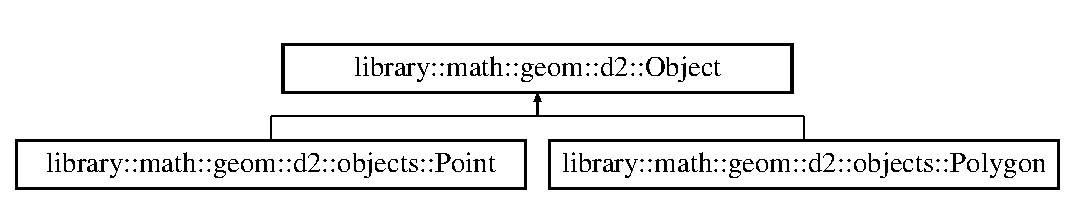
\includegraphics[height=0.569395cm]{classlibrary_1_1math_1_1geom_1_1d2_1_1_object}
\end{center}
\end{figure}
\subsection*{Public Types}
\begin{DoxyCompactItemize}
\item 
enum \hyperlink{classlibrary_1_1math_1_1geom_1_1d2_1_1_object_ac8cd61dada4960cfee9a469231621b17}{Format} \{ \hyperlink{classlibrary_1_1math_1_1geom_1_1d2_1_1_object_ac8cd61dada4960cfee9a469231621b17aec0fc0100c4fc1ce4eea230c3dc10360}{Format\+::\+Undefined}, 
\hyperlink{classlibrary_1_1math_1_1geom_1_1d2_1_1_object_ac8cd61dada4960cfee9a469231621b17aeb6d8ae6f20283755b339c0dc273988b}{Format\+::\+Standard}, 
\hyperlink{classlibrary_1_1math_1_1geom_1_1d2_1_1_object_ac8cd61dada4960cfee9a469231621b17a9ab05752e6beff2c783a6046ed592661}{Format\+::\+W\+KT}
 \}
\end{DoxyCompactItemize}
\subsection*{Public Member Functions}
\begin{DoxyCompactItemize}
\item 
\hyperlink{classlibrary_1_1math_1_1geom_1_1d2_1_1_object_a35b722f64aded8d8e660074a23af237a}{Object} ()=default
\begin{DoxyCompactList}\small\item\em Default constructor. \end{DoxyCompactList}\item 
virtual \hyperlink{classlibrary_1_1math_1_1geom_1_1d2_1_1_object_a092ca69d924f7226fceeb35f5532887c}{$\sim$\+Object} ()=0
\begin{DoxyCompactList}\small\item\em Destructor (pure virtual) \end{DoxyCompactList}\item 
virtual \hyperlink{classlibrary_1_1math_1_1geom_1_1d2_1_1_object}{Object} $\ast$ \hyperlink{classlibrary_1_1math_1_1geom_1_1d2_1_1_object_a5c26ae4120edb24f6463d65a9cef247d}{clone} () const =0
\begin{DoxyCompactList}\small\item\em Clone object (pure virtual) \end{DoxyCompactList}\item 
bool \hyperlink{classlibrary_1_1math_1_1geom_1_1d2_1_1_object_a97aeb08c0dbe7f803188ae335f6b0e7a}{operator==} (const \hyperlink{classlibrary_1_1math_1_1geom_1_1d2_1_1_object}{Object} \&an\+Object) const
\begin{DoxyCompactList}\small\item\em Not equal to operator. \end{DoxyCompactList}\item 
bool \hyperlink{classlibrary_1_1math_1_1geom_1_1d2_1_1_object_a538fa27124314cddf9705cf35a3efc08}{operator!=} (const \hyperlink{classlibrary_1_1math_1_1geom_1_1d2_1_1_object}{Object} \&an\+Object) const
\begin{DoxyCompactList}\small\item\em Not equal to operator. \end{DoxyCompactList}\item 
virtual bool \hyperlink{classlibrary_1_1math_1_1geom_1_1d2_1_1_object_ae9506254971168a3ca63e1923556b70d}{is\+Defined} () const =0
\begin{DoxyCompactList}\small\item\em Check if object is defined. \end{DoxyCompactList}\item 
virtual bool \hyperlink{classlibrary_1_1math_1_1geom_1_1d2_1_1_object_a22819b510e52283c19c4ed947e0cba97}{intersects} (const \hyperlink{classlibrary_1_1math_1_1geom_1_1d2_1_1_object}{Object} \&an\+Object) const
\begin{DoxyCompactList}\small\item\em Check if object intersects another object. \end{DoxyCompactList}\item 
virtual bool \hyperlink{classlibrary_1_1math_1_1geom_1_1d2_1_1_object_a7bc14e621db51aec72eff0fa5da295ac}{contains} (const \hyperlink{classlibrary_1_1math_1_1geom_1_1d2_1_1_object}{Object} \&an\+Object) const
\begin{DoxyCompactList}\small\item\em Check if object contains another object. \end{DoxyCompactList}\item 
virtual String \hyperlink{classlibrary_1_1math_1_1geom_1_1d2_1_1_object_acdd76b3637732a249536b609dbe3f0eb}{to\+String} (const \hyperlink{classlibrary_1_1math_1_1geom_1_1d2_1_1_object_ac8cd61dada4960cfee9a469231621b17}{Object\+::\+Format} \&a\+Format=\hyperlink{classlibrary_1_1math_1_1geom_1_1d2_1_1_object_ac8cd61dada4960cfee9a469231621b17aeb6d8ae6f20283755b339c0dc273988b}{Object\+::\+Format\+::\+Standard}, const Integer \&a\+Precision=Integer\+::\+Undefined()) const =0
\begin{DoxyCompactList}\small\item\em Get string representation. \end{DoxyCompactList}\item 
virtual void \hyperlink{classlibrary_1_1math_1_1geom_1_1d2_1_1_object_a834bbf59cf1c483d1dc7b0966b1e1ab3}{print} (std\+::ostream \&an\+Output\+Stream, bool display\+Decorators=true) const =0
\begin{DoxyCompactList}\small\item\em Print object. \end{DoxyCompactList}\item 
virtual void \hyperlink{classlibrary_1_1math_1_1geom_1_1d2_1_1_object_a289589fb6e9e7a2c4ca4976a1544def5}{apply\+Transformation} (const \hyperlink{classlibrary_1_1math_1_1geom_1_1d2_1_1_transformation}{Transformation} \&a\+Transformation)=0
\begin{DoxyCompactList}\small\item\em Apply transformation to object. \end{DoxyCompactList}\end{DoxyCompactItemize}
\subsection*{Friends}
\begin{DoxyCompactItemize}
\item 
std\+::ostream \& \hyperlink{classlibrary_1_1math_1_1geom_1_1d2_1_1_object_a418df9bf4a73078f3d494edef1743f8d}{operator$<$$<$} (std\+::ostream \&an\+Output\+Stream, const \hyperlink{classlibrary_1_1math_1_1geom_1_1d2_1_1_object}{Object} \&an\+Object)
\begin{DoxyCompactList}\small\item\em Output stream operator. \end{DoxyCompactList}\end{DoxyCompactItemize}


\subsection{Detailed Description}
2D object 

\subsection{Member Enumeration Documentation}
\mbox{\Hypertarget{classlibrary_1_1math_1_1geom_1_1d2_1_1_object_ac8cd61dada4960cfee9a469231621b17}\label{classlibrary_1_1math_1_1geom_1_1d2_1_1_object_ac8cd61dada4960cfee9a469231621b17}} 
\index{library\+::math\+::geom\+::d2\+::\+Object@{library\+::math\+::geom\+::d2\+::\+Object}!Format@{Format}}
\index{Format@{Format}!library\+::math\+::geom\+::d2\+::\+Object@{library\+::math\+::geom\+::d2\+::\+Object}}
\subsubsection{\texorpdfstring{Format}{Format}}
{\footnotesize\ttfamily enum \hyperlink{classlibrary_1_1math_1_1geom_1_1d2_1_1_object_ac8cd61dada4960cfee9a469231621b17}{library\+::math\+::geom\+::d2\+::\+Object\+::\+Format}\hspace{0.3cm}{\ttfamily [strong]}}

\begin{DoxyEnumFields}{Enumerator}
\raisebox{\heightof{T}}[0pt][0pt]{\index{Undefined@{Undefined}!library\+::math\+::geom\+::d2\+::\+Object@{library\+::math\+::geom\+::d2\+::\+Object}}\index{library\+::math\+::geom\+::d2\+::\+Object@{library\+::math\+::geom\+::d2\+::\+Object}!Undefined@{Undefined}}}\mbox{\Hypertarget{classlibrary_1_1math_1_1geom_1_1d2_1_1_object_ac8cd61dada4960cfee9a469231621b17aec0fc0100c4fc1ce4eea230c3dc10360}\label{classlibrary_1_1math_1_1geom_1_1d2_1_1_object_ac8cd61dada4960cfee9a469231621b17aec0fc0100c4fc1ce4eea230c3dc10360}} 
Undefined&Undefined format. \\
\hline

\raisebox{\heightof{T}}[0pt][0pt]{\index{Standard@{Standard}!library\+::math\+::geom\+::d2\+::\+Object@{library\+::math\+::geom\+::d2\+::\+Object}}\index{library\+::math\+::geom\+::d2\+::\+Object@{library\+::math\+::geom\+::d2\+::\+Object}!Standard@{Standard}}}\mbox{\Hypertarget{classlibrary_1_1math_1_1geom_1_1d2_1_1_object_ac8cd61dada4960cfee9a469231621b17aeb6d8ae6f20283755b339c0dc273988b}\label{classlibrary_1_1math_1_1geom_1_1d2_1_1_object_ac8cd61dada4960cfee9a469231621b17aeb6d8ae6f20283755b339c0dc273988b}} 
Standard&Standard format. \\
\hline

\raisebox{\heightof{T}}[0pt][0pt]{\index{W\+KT@{W\+KT}!library\+::math\+::geom\+::d2\+::\+Object@{library\+::math\+::geom\+::d2\+::\+Object}}\index{library\+::math\+::geom\+::d2\+::\+Object@{library\+::math\+::geom\+::d2\+::\+Object}!W\+KT@{W\+KT}}}\mbox{\Hypertarget{classlibrary_1_1math_1_1geom_1_1d2_1_1_object_ac8cd61dada4960cfee9a469231621b17a9ab05752e6beff2c783a6046ed592661}\label{classlibrary_1_1math_1_1geom_1_1d2_1_1_object_ac8cd61dada4960cfee9a469231621b17a9ab05752e6beff2c783a6046ed592661}} 
W\+KT&Well-\/\+Known Text (W\+KT) format. \\
\hline

\end{DoxyEnumFields}


\subsection{Constructor \& Destructor Documentation}
\mbox{\Hypertarget{classlibrary_1_1math_1_1geom_1_1d2_1_1_object_a35b722f64aded8d8e660074a23af237a}\label{classlibrary_1_1math_1_1geom_1_1d2_1_1_object_a35b722f64aded8d8e660074a23af237a}} 
\index{library\+::math\+::geom\+::d2\+::\+Object@{library\+::math\+::geom\+::d2\+::\+Object}!Object@{Object}}
\index{Object@{Object}!library\+::math\+::geom\+::d2\+::\+Object@{library\+::math\+::geom\+::d2\+::\+Object}}
\subsubsection{\texorpdfstring{Object()}{Object()}}
{\footnotesize\ttfamily library\+::math\+::geom\+::d2\+::\+Object\+::\+Object (\begin{DoxyParamCaption}{ }\end{DoxyParamCaption})\hspace{0.3cm}{\ttfamily [default]}}



Default constructor. 

\mbox{\Hypertarget{classlibrary_1_1math_1_1geom_1_1d2_1_1_object_a092ca69d924f7226fceeb35f5532887c}\label{classlibrary_1_1math_1_1geom_1_1d2_1_1_object_a092ca69d924f7226fceeb35f5532887c}} 
\index{library\+::math\+::geom\+::d2\+::\+Object@{library\+::math\+::geom\+::d2\+::\+Object}!````~Object@{$\sim$\+Object}}
\index{````~Object@{$\sim$\+Object}!library\+::math\+::geom\+::d2\+::\+Object@{library\+::math\+::geom\+::d2\+::\+Object}}
\subsubsection{\texorpdfstring{$\sim$\+Object()}{~Object()}}
{\footnotesize\ttfamily library\+::math\+::geom\+::d2\+::\+Object\+::$\sim$\+Object (\begin{DoxyParamCaption}{ }\end{DoxyParamCaption})\hspace{0.3cm}{\ttfamily [pure virtual]}}



Destructor (pure virtual) 



\subsection{Member Function Documentation}
\mbox{\Hypertarget{classlibrary_1_1math_1_1geom_1_1d2_1_1_object_a289589fb6e9e7a2c4ca4976a1544def5}\label{classlibrary_1_1math_1_1geom_1_1d2_1_1_object_a289589fb6e9e7a2c4ca4976a1544def5}} 
\index{library\+::math\+::geom\+::d2\+::\+Object@{library\+::math\+::geom\+::d2\+::\+Object}!apply\+Transformation@{apply\+Transformation}}
\index{apply\+Transformation@{apply\+Transformation}!library\+::math\+::geom\+::d2\+::\+Object@{library\+::math\+::geom\+::d2\+::\+Object}}
\subsubsection{\texorpdfstring{apply\+Transformation()}{applyTransformation()}}
{\footnotesize\ttfamily virtual void library\+::math\+::geom\+::d2\+::\+Object\+::apply\+Transformation (\begin{DoxyParamCaption}\item[{const \hyperlink{classlibrary_1_1math_1_1geom_1_1d2_1_1_transformation}{Transformation} \&}]{a\+Transformation }\end{DoxyParamCaption})\hspace{0.3cm}{\ttfamily [pure virtual]}}



Apply transformation to object. 


\begin{DoxyParams}[1]{Parameters}
\mbox{\tt in}  & {\em a\+Transformation} & A transformation \\
\hline
\end{DoxyParams}


Implemented in \hyperlink{classlibrary_1_1math_1_1geom_1_1d2_1_1objects_1_1_polygon_a920b30eb110c7164f65754979da17638}{library\+::math\+::geom\+::d2\+::objects\+::\+Polygon}, \hyperlink{classlibrary_1_1math_1_1geom_1_1d2_1_1objects_1_1_segment_a5cb71beeb4de3c2c1b84fbfb8546c935}{library\+::math\+::geom\+::d2\+::objects\+::\+Segment}, \hyperlink{classlibrary_1_1math_1_1geom_1_1d2_1_1objects_1_1_point_set_acfb8652fd1f17f101e7750a0b81452c0}{library\+::math\+::geom\+::d2\+::objects\+::\+Point\+Set}, \hyperlink{classlibrary_1_1math_1_1geom_1_1d2_1_1objects_1_1_point_a71d3ef79dbffcd2568d1a2c6bad807d7}{library\+::math\+::geom\+::d2\+::objects\+::\+Point}, \hyperlink{classlibrary_1_1math_1_1geom_1_1d2_1_1objects_1_1_line_string_abd9e77eb0e1d319e8f9af23ccb6dc0b4}{library\+::math\+::geom\+::d2\+::objects\+::\+Line\+String}, \hyperlink{classlibrary_1_1math_1_1geom_1_1d2_1_1objects_1_1_multi_polygon_af4adcde904edd77d54236517652e4da1}{library\+::math\+::geom\+::d2\+::objects\+::\+Multi\+Polygon}, and \hyperlink{classlibrary_1_1math_1_1geom_1_1d2_1_1objects_1_1_multi_line_string_a6180a8b94ff175d6313a74ad4e680bc7}{library\+::math\+::geom\+::d2\+::objects\+::\+Multi\+Line\+String}.

\mbox{\Hypertarget{classlibrary_1_1math_1_1geom_1_1d2_1_1_object_a5c26ae4120edb24f6463d65a9cef247d}\label{classlibrary_1_1math_1_1geom_1_1d2_1_1_object_a5c26ae4120edb24f6463d65a9cef247d}} 
\index{library\+::math\+::geom\+::d2\+::\+Object@{library\+::math\+::geom\+::d2\+::\+Object}!clone@{clone}}
\index{clone@{clone}!library\+::math\+::geom\+::d2\+::\+Object@{library\+::math\+::geom\+::d2\+::\+Object}}
\subsubsection{\texorpdfstring{clone()}{clone()}}
{\footnotesize\ttfamily virtual \hyperlink{classlibrary_1_1math_1_1geom_1_1d2_1_1_object}{Object}$\ast$ library\+::math\+::geom\+::d2\+::\+Object\+::clone (\begin{DoxyParamCaption}{ }\end{DoxyParamCaption}) const\hspace{0.3cm}{\ttfamily [pure virtual]}}



Clone object (pure virtual) 

\begin{DoxyReturn}{Returns}
Pointer to cloned object 
\end{DoxyReturn}


Implemented in \hyperlink{classlibrary_1_1math_1_1geom_1_1d2_1_1objects_1_1_polygon_a15bbbe7e468a50d6059e2df946175e1c}{library\+::math\+::geom\+::d2\+::objects\+::\+Polygon}, \hyperlink{classlibrary_1_1math_1_1geom_1_1d2_1_1objects_1_1_point_set_ad867c4fb86734efe968a39c95eba53b3}{library\+::math\+::geom\+::d2\+::objects\+::\+Point\+Set}, \hyperlink{classlibrary_1_1math_1_1geom_1_1d2_1_1objects_1_1_multi_polygon_a6dc8db614de9fb615491deb783fe7fcd}{library\+::math\+::geom\+::d2\+::objects\+::\+Multi\+Polygon}, \hyperlink{classlibrary_1_1math_1_1geom_1_1d2_1_1objects_1_1_line_string_a5b503802b279c6c305fed6a07a893ad2}{library\+::math\+::geom\+::d2\+::objects\+::\+Line\+String}, \hyperlink{classlibrary_1_1math_1_1geom_1_1d2_1_1objects_1_1_multi_line_string_a38054f0f0a2c198b5d3c76ef22562e30}{library\+::math\+::geom\+::d2\+::objects\+::\+Multi\+Line\+String}, \hyperlink{classlibrary_1_1math_1_1geom_1_1d2_1_1objects_1_1_segment_a6149a3cf215b0b573d5bd4f25fad75e9}{library\+::math\+::geom\+::d2\+::objects\+::\+Segment}, and \hyperlink{classlibrary_1_1math_1_1geom_1_1d2_1_1objects_1_1_point_aa6b55bdbf5a0ce9ec8bc91ca79de3569}{library\+::math\+::geom\+::d2\+::objects\+::\+Point}.

\mbox{\Hypertarget{classlibrary_1_1math_1_1geom_1_1d2_1_1_object_a7bc14e621db51aec72eff0fa5da295ac}\label{classlibrary_1_1math_1_1geom_1_1d2_1_1_object_a7bc14e621db51aec72eff0fa5da295ac}} 
\index{library\+::math\+::geom\+::d2\+::\+Object@{library\+::math\+::geom\+::d2\+::\+Object}!contains@{contains}}
\index{contains@{contains}!library\+::math\+::geom\+::d2\+::\+Object@{library\+::math\+::geom\+::d2\+::\+Object}}
\subsubsection{\texorpdfstring{contains()}{contains()}}
{\footnotesize\ttfamily bool library\+::math\+::geom\+::d2\+::\+Object\+::contains (\begin{DoxyParamCaption}\item[{const \hyperlink{classlibrary_1_1math_1_1geom_1_1d2_1_1_object}{Object} \&}]{an\+Object }\end{DoxyParamCaption}) const\hspace{0.3cm}{\ttfamily [virtual]}}



Check if object contains another object. 


\begin{DoxyCode}
Unique<Object> objectUPtr = ... ;
Unique<Object> anotherObjectUPtr = ... ;
objectUPtr->contains(*anotherObjectUPtr) ;
\end{DoxyCode}



\begin{DoxyParams}[1]{Parameters}
\mbox{\tt in}  & {\em an\+Object} & An object \\
\hline
\end{DoxyParams}
\begin{DoxyReturn}{Returns}
True if object contains another object 
\end{DoxyReturn}
\mbox{\Hypertarget{classlibrary_1_1math_1_1geom_1_1d2_1_1_object_a22819b510e52283c19c4ed947e0cba97}\label{classlibrary_1_1math_1_1geom_1_1d2_1_1_object_a22819b510e52283c19c4ed947e0cba97}} 
\index{library\+::math\+::geom\+::d2\+::\+Object@{library\+::math\+::geom\+::d2\+::\+Object}!intersects@{intersects}}
\index{intersects@{intersects}!library\+::math\+::geom\+::d2\+::\+Object@{library\+::math\+::geom\+::d2\+::\+Object}}
\subsubsection{\texorpdfstring{intersects()}{intersects()}}
{\footnotesize\ttfamily bool library\+::math\+::geom\+::d2\+::\+Object\+::intersects (\begin{DoxyParamCaption}\item[{const \hyperlink{classlibrary_1_1math_1_1geom_1_1d2_1_1_object}{Object} \&}]{an\+Object }\end{DoxyParamCaption}) const\hspace{0.3cm}{\ttfamily [virtual]}}



Check if object intersects another object. 


\begin{DoxyCode}
Unique<Object> objectUPtr = ... ;
Unique<Object> anotherObjectUPtr = ... ;
objectUPtr->intersects(*anotherObjectUPtr) ;
\end{DoxyCode}



\begin{DoxyParams}[1]{Parameters}
\mbox{\tt in}  & {\em an\+Object} & An object \\
\hline
\end{DoxyParams}
\begin{DoxyReturn}{Returns}
True if object intersects another object 
\end{DoxyReturn}
\mbox{\Hypertarget{classlibrary_1_1math_1_1geom_1_1d2_1_1_object_ae9506254971168a3ca63e1923556b70d}\label{classlibrary_1_1math_1_1geom_1_1d2_1_1_object_ae9506254971168a3ca63e1923556b70d}} 
\index{library\+::math\+::geom\+::d2\+::\+Object@{library\+::math\+::geom\+::d2\+::\+Object}!is\+Defined@{is\+Defined}}
\index{is\+Defined@{is\+Defined}!library\+::math\+::geom\+::d2\+::\+Object@{library\+::math\+::geom\+::d2\+::\+Object}}
\subsubsection{\texorpdfstring{is\+Defined()}{isDefined()}}
{\footnotesize\ttfamily virtual bool library\+::math\+::geom\+::d2\+::\+Object\+::is\+Defined (\begin{DoxyParamCaption}{ }\end{DoxyParamCaption}) const\hspace{0.3cm}{\ttfamily [pure virtual]}}



Check if object is defined. 

\begin{DoxyReturn}{Returns}
True if object is defined 
\end{DoxyReturn}


Implemented in \hyperlink{classlibrary_1_1math_1_1geom_1_1d2_1_1objects_1_1_polygon_a83e0962f91f0732048e156ad634faaea}{library\+::math\+::geom\+::d2\+::objects\+::\+Polygon}, \hyperlink{classlibrary_1_1math_1_1geom_1_1d2_1_1objects_1_1_point_ac90251968d8eb11df82e28f6cf095e5c}{library\+::math\+::geom\+::d2\+::objects\+::\+Point}, \hyperlink{classlibrary_1_1math_1_1geom_1_1d2_1_1objects_1_1_point_set_a031a6b5688c65bce8f37af452c0f0959}{library\+::math\+::geom\+::d2\+::objects\+::\+Point\+Set}, \hyperlink{classlibrary_1_1math_1_1geom_1_1d2_1_1objects_1_1_multi_polygon_a9afa806e12102255fc5abf8a94106089}{library\+::math\+::geom\+::d2\+::objects\+::\+Multi\+Polygon}, \hyperlink{classlibrary_1_1math_1_1geom_1_1d2_1_1objects_1_1_segment_a2c366d74328cdce4a7e83a761a84dbc7}{library\+::math\+::geom\+::d2\+::objects\+::\+Segment}, \hyperlink{classlibrary_1_1math_1_1geom_1_1d2_1_1objects_1_1_line_string_a2ef4a1e387ed463286fac7c93fd7b022}{library\+::math\+::geom\+::d2\+::objects\+::\+Line\+String}, and \hyperlink{classlibrary_1_1math_1_1geom_1_1d2_1_1objects_1_1_multi_line_string_a77de687b2c287226984e2614dafe744a}{library\+::math\+::geom\+::d2\+::objects\+::\+Multi\+Line\+String}.

\mbox{\Hypertarget{classlibrary_1_1math_1_1geom_1_1d2_1_1_object_a538fa27124314cddf9705cf35a3efc08}\label{classlibrary_1_1math_1_1geom_1_1d2_1_1_object_a538fa27124314cddf9705cf35a3efc08}} 
\index{library\+::math\+::geom\+::d2\+::\+Object@{library\+::math\+::geom\+::d2\+::\+Object}!operator"!=@{operator"!=}}
\index{operator"!=@{operator"!=}!library\+::math\+::geom\+::d2\+::\+Object@{library\+::math\+::geom\+::d2\+::\+Object}}
\subsubsection{\texorpdfstring{operator"!=()}{operator!=()}}
{\footnotesize\ttfamily bool library\+::math\+::geom\+::d2\+::\+Object\+::operator!= (\begin{DoxyParamCaption}\item[{const \hyperlink{classlibrary_1_1math_1_1geom_1_1d2_1_1_object}{Object} \&}]{an\+Object }\end{DoxyParamCaption}) const}



Not equal to operator. 


\begin{DoxyParams}[1]{Parameters}
\mbox{\tt in}  & {\em an\+Object} & An object \\
\hline
\end{DoxyParams}
\begin{DoxyReturn}{Returns}
True if objects are not equal 
\end{DoxyReturn}
\mbox{\Hypertarget{classlibrary_1_1math_1_1geom_1_1d2_1_1_object_a97aeb08c0dbe7f803188ae335f6b0e7a}\label{classlibrary_1_1math_1_1geom_1_1d2_1_1_object_a97aeb08c0dbe7f803188ae335f6b0e7a}} 
\index{library\+::math\+::geom\+::d2\+::\+Object@{library\+::math\+::geom\+::d2\+::\+Object}!operator==@{operator==}}
\index{operator==@{operator==}!library\+::math\+::geom\+::d2\+::\+Object@{library\+::math\+::geom\+::d2\+::\+Object}}
\subsubsection{\texorpdfstring{operator==()}{operator==()}}
{\footnotesize\ttfamily bool library\+::math\+::geom\+::d2\+::\+Object\+::operator== (\begin{DoxyParamCaption}\item[{const \hyperlink{classlibrary_1_1math_1_1geom_1_1d2_1_1_object}{Object} \&}]{an\+Object }\end{DoxyParamCaption}) const}



Not equal to operator. 


\begin{DoxyParams}[1]{Parameters}
\mbox{\tt in}  & {\em an\+Object} & An object \\
\hline
\end{DoxyParams}
\begin{DoxyReturn}{Returns}
True if objects are equal 
\end{DoxyReturn}
\mbox{\Hypertarget{classlibrary_1_1math_1_1geom_1_1d2_1_1_object_a834bbf59cf1c483d1dc7b0966b1e1ab3}\label{classlibrary_1_1math_1_1geom_1_1d2_1_1_object_a834bbf59cf1c483d1dc7b0966b1e1ab3}} 
\index{library\+::math\+::geom\+::d2\+::\+Object@{library\+::math\+::geom\+::d2\+::\+Object}!print@{print}}
\index{print@{print}!library\+::math\+::geom\+::d2\+::\+Object@{library\+::math\+::geom\+::d2\+::\+Object}}
\subsubsection{\texorpdfstring{print()}{print()}}
{\footnotesize\ttfamily virtual void library\+::math\+::geom\+::d2\+::\+Object\+::print (\begin{DoxyParamCaption}\item[{std\+::ostream \&}]{an\+Output\+Stream,  }\item[{bool}]{display\+Decorators = {\ttfamily true} }\end{DoxyParamCaption}) const\hspace{0.3cm}{\ttfamily [pure virtual]}}



Print object. 


\begin{DoxyParams}[1]{Parameters}
\mbox{\tt in}  & {\em an\+Output\+Stream} & An output stream \\
\hline
\mbox{\tt in}  & {\em (optional)} & display\+Decorators If true, display decorators \\
\hline
\end{DoxyParams}


Implemented in \hyperlink{classlibrary_1_1math_1_1geom_1_1d2_1_1objects_1_1_polygon_a028ca7818387654ed1aab1584cee6cc5}{library\+::math\+::geom\+::d2\+::objects\+::\+Polygon}, \hyperlink{classlibrary_1_1math_1_1geom_1_1d2_1_1objects_1_1_segment_abfe0b4983dcb9e26848d29a9b86d4b9c}{library\+::math\+::geom\+::d2\+::objects\+::\+Segment}, \hyperlink{classlibrary_1_1math_1_1geom_1_1d2_1_1objects_1_1_point_a74bef6325d728e1cb6e70bac0b8d4601}{library\+::math\+::geom\+::d2\+::objects\+::\+Point}, \hyperlink{classlibrary_1_1math_1_1geom_1_1d2_1_1objects_1_1_point_set_a652098938854c19294b5df8e8634cc9a}{library\+::math\+::geom\+::d2\+::objects\+::\+Point\+Set}, \hyperlink{classlibrary_1_1math_1_1geom_1_1d2_1_1objects_1_1_multi_polygon_aa1998e9d86d24edb61e978f397148d1c}{library\+::math\+::geom\+::d2\+::objects\+::\+Multi\+Polygon}, \hyperlink{classlibrary_1_1math_1_1geom_1_1d2_1_1objects_1_1_line_string_ae980ac86d1f2d8091151252aef2b6adc}{library\+::math\+::geom\+::d2\+::objects\+::\+Line\+String}, and \hyperlink{classlibrary_1_1math_1_1geom_1_1d2_1_1objects_1_1_multi_line_string_ab7854c1006501bf5159b890a662198b1}{library\+::math\+::geom\+::d2\+::objects\+::\+Multi\+Line\+String}.

\mbox{\Hypertarget{classlibrary_1_1math_1_1geom_1_1d2_1_1_object_acdd76b3637732a249536b609dbe3f0eb}\label{classlibrary_1_1math_1_1geom_1_1d2_1_1_object_acdd76b3637732a249536b609dbe3f0eb}} 
\index{library\+::math\+::geom\+::d2\+::\+Object@{library\+::math\+::geom\+::d2\+::\+Object}!to\+String@{to\+String}}
\index{to\+String@{to\+String}!library\+::math\+::geom\+::d2\+::\+Object@{library\+::math\+::geom\+::d2\+::\+Object}}
\subsubsection{\texorpdfstring{to\+String()}{toString()}}
{\footnotesize\ttfamily virtual String library\+::math\+::geom\+::d2\+::\+Object\+::to\+String (\begin{DoxyParamCaption}\item[{const \hyperlink{classlibrary_1_1math_1_1geom_1_1d2_1_1_object_ac8cd61dada4960cfee9a469231621b17}{Object\+::\+Format} \&}]{a\+Format = {\ttfamily \hyperlink{classlibrary_1_1math_1_1geom_1_1d2_1_1_object_ac8cd61dada4960cfee9a469231621b17aeb6d8ae6f20283755b339c0dc273988b}{Object\+::\+Format\+::\+Standard}},  }\item[{const Integer \&}]{a\+Precision = {\ttfamily Integer\+:\+:Undefined()} }\end{DoxyParamCaption}) const\hspace{0.3cm}{\ttfamily [pure virtual]}}



Get string representation. 


\begin{DoxyParams}[1]{Parameters}
\mbox{\tt in}  & {\em a\+Format} & A format \\
\hline
\end{DoxyParams}
\begin{DoxyReturn}{Returns}
String representation 
\end{DoxyReturn}


Implemented in \hyperlink{classlibrary_1_1math_1_1geom_1_1d2_1_1objects_1_1_polygon_acef17857f29323e985fba23441ed1171}{library\+::math\+::geom\+::d2\+::objects\+::\+Polygon}, \hyperlink{classlibrary_1_1math_1_1geom_1_1d2_1_1objects_1_1_segment_a6efb82e3e5e5d97214b827bc6f8574e3}{library\+::math\+::geom\+::d2\+::objects\+::\+Segment}, \hyperlink{classlibrary_1_1math_1_1geom_1_1d2_1_1objects_1_1_point_ae645a37f426dac123d566fb5511d595d}{library\+::math\+::geom\+::d2\+::objects\+::\+Point}, \hyperlink{classlibrary_1_1math_1_1geom_1_1d2_1_1objects_1_1_point_set_a4eeece63192481627cb0f991a4eef1a4}{library\+::math\+::geom\+::d2\+::objects\+::\+Point\+Set}, \hyperlink{classlibrary_1_1math_1_1geom_1_1d2_1_1objects_1_1_multi_polygon_a598e024d69ca9a99d97cf7412b334869}{library\+::math\+::geom\+::d2\+::objects\+::\+Multi\+Polygon}, \hyperlink{classlibrary_1_1math_1_1geom_1_1d2_1_1objects_1_1_line_string_a13c0a7c5b8da7724b5a2dd2933064768}{library\+::math\+::geom\+::d2\+::objects\+::\+Line\+String}, and \hyperlink{classlibrary_1_1math_1_1geom_1_1d2_1_1objects_1_1_multi_line_string_a71d1e434196bb8d67054ad28d8aa59a6}{library\+::math\+::geom\+::d2\+::objects\+::\+Multi\+Line\+String}.



\subsection{Friends And Related Function Documentation}
\mbox{\Hypertarget{classlibrary_1_1math_1_1geom_1_1d2_1_1_object_a418df9bf4a73078f3d494edef1743f8d}\label{classlibrary_1_1math_1_1geom_1_1d2_1_1_object_a418df9bf4a73078f3d494edef1743f8d}} 
\index{library\+::math\+::geom\+::d2\+::\+Object@{library\+::math\+::geom\+::d2\+::\+Object}!operator$<$$<$@{operator$<$$<$}}
\index{operator$<$$<$@{operator$<$$<$}!library\+::math\+::geom\+::d2\+::\+Object@{library\+::math\+::geom\+::d2\+::\+Object}}
\subsubsection{\texorpdfstring{operator$<$$<$}{operator<<}}
{\footnotesize\ttfamily std\+::ostream\& operator$<$$<$ (\begin{DoxyParamCaption}\item[{std\+::ostream \&}]{an\+Output\+Stream,  }\item[{const \hyperlink{classlibrary_1_1math_1_1geom_1_1d2_1_1_object}{Object} \&}]{an\+Object }\end{DoxyParamCaption})\hspace{0.3cm}{\ttfamily [friend]}}



Output stream operator. 


\begin{DoxyParams}[1]{Parameters}
\mbox{\tt in}  & {\em an\+Output\+Stream} & An output stream \\
\hline
\mbox{\tt in}  & {\em an\+Object} & An object \\
\hline
\end{DoxyParams}
\begin{DoxyReturn}{Returns}
A reference to output stream 
\end{DoxyReturn}


The documentation for this class was generated from the following files\+:\begin{DoxyCompactItemize}
\item 
include/\+Library/\+Mathematics/\+Geometry/2\+D/\hyperlink{2_d_2_object_8hpp}{Object.\+hpp}\item 
src/\+Library/\+Mathematics/\+Geometry/2\+D/\hyperlink{2_d_2_object_8cpp}{Object.\+cpp}\end{DoxyCompactItemize}

\hypertarget{classlibrary_1_1math_1_1geom_1_1d3_1_1_object}{}\section{library\+:\+:math\+:\+:geom\+:\+:d3\+:\+:Object Class Reference}
\label{classlibrary_1_1math_1_1geom_1_1d3_1_1_object}\index{library\+::math\+::geom\+::d3\+::\+Object@{library\+::math\+::geom\+::d3\+::\+Object}}


3D object  




{\ttfamily \#include $<$Object.\+hpp$>$}

Inheritance diagram for library\+:\+:math\+:\+:geom\+:\+:d3\+:\+:Object\+:\begin{figure}[H]
\begin{center}
\leavevmode
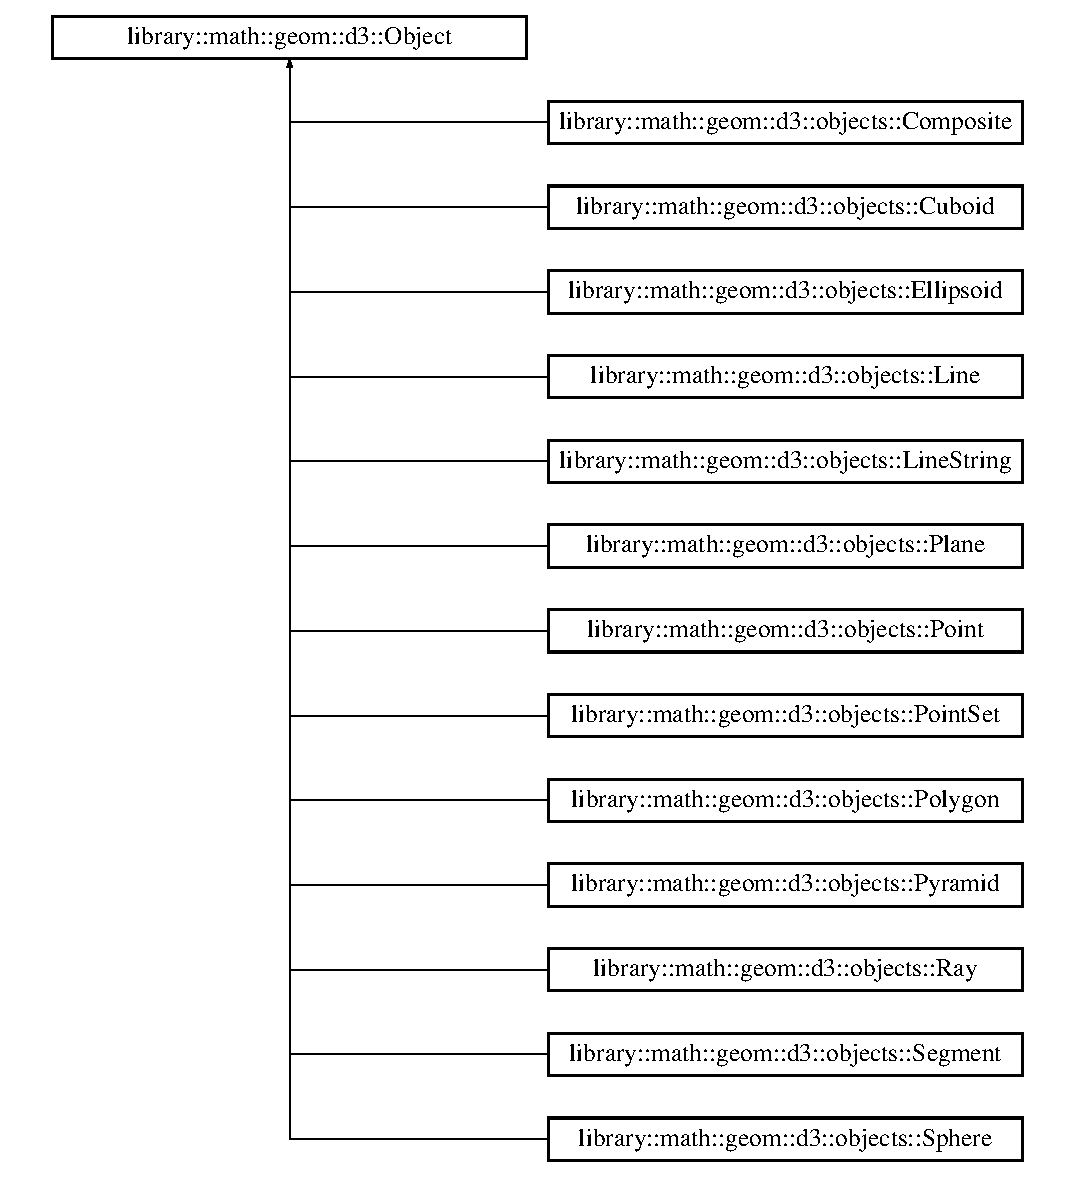
\includegraphics[height=1.530055cm]{classlibrary_1_1math_1_1geom_1_1d3_1_1_object}
\end{center}
\end{figure}
\subsection*{Public Member Functions}
\begin{DoxyCompactItemize}
\item 
\hyperlink{classlibrary_1_1math_1_1geom_1_1d3_1_1_object_ab484354bbce44290b6d288c7825d9e42}{Object} ()=default
\begin{DoxyCompactList}\small\item\em Default constructor. \end{DoxyCompactList}\item 
virtual \hyperlink{classlibrary_1_1math_1_1geom_1_1d3_1_1_object_addfda217130395f6eeb080a2fe406876}{$\sim$\+Object} ()=0
\begin{DoxyCompactList}\small\item\em Destructor (pure virtual) \end{DoxyCompactList}\item 
virtual \hyperlink{classlibrary_1_1math_1_1geom_1_1d3_1_1_object}{Object} $\ast$ \hyperlink{classlibrary_1_1math_1_1geom_1_1d3_1_1_object_a1a784c6b359e0eb97cd34fabc42f2f3f}{clone} () const =0
\begin{DoxyCompactList}\small\item\em Clone object (pure virtual) \end{DoxyCompactList}\item 
virtual bool \hyperlink{classlibrary_1_1math_1_1geom_1_1d3_1_1_object_a2216442e322f0c3ca5f01a4efa22baf7}{is\+Defined} () const =0
\begin{DoxyCompactList}\small\item\em Check if object is defined. \end{DoxyCompactList}\end{DoxyCompactItemize}


\subsection{Detailed Description}
3D object 

\subsection{Constructor \& Destructor Documentation}
\mbox{\Hypertarget{classlibrary_1_1math_1_1geom_1_1d3_1_1_object_ab484354bbce44290b6d288c7825d9e42}\label{classlibrary_1_1math_1_1geom_1_1d3_1_1_object_ab484354bbce44290b6d288c7825d9e42}} 
\index{library\+::math\+::geom\+::d3\+::\+Object@{library\+::math\+::geom\+::d3\+::\+Object}!Object@{Object}}
\index{Object@{Object}!library\+::math\+::geom\+::d3\+::\+Object@{library\+::math\+::geom\+::d3\+::\+Object}}
\subsubsection{\texorpdfstring{Object()}{Object()}}
{\footnotesize\ttfamily library\+::math\+::geom\+::d3\+::\+Object\+::\+Object (\begin{DoxyParamCaption}{ }\end{DoxyParamCaption})\hspace{0.3cm}{\ttfamily [default]}}



Default constructor. 

\mbox{\Hypertarget{classlibrary_1_1math_1_1geom_1_1d3_1_1_object_addfda217130395f6eeb080a2fe406876}\label{classlibrary_1_1math_1_1geom_1_1d3_1_1_object_addfda217130395f6eeb080a2fe406876}} 
\index{library\+::math\+::geom\+::d3\+::\+Object@{library\+::math\+::geom\+::d3\+::\+Object}!````~Object@{$\sim$\+Object}}
\index{````~Object@{$\sim$\+Object}!library\+::math\+::geom\+::d3\+::\+Object@{library\+::math\+::geom\+::d3\+::\+Object}}
\subsubsection{\texorpdfstring{$\sim$\+Object()}{~Object()}}
{\footnotesize\ttfamily library\+::math\+::geom\+::d3\+::\+Object\+::$\sim$\+Object (\begin{DoxyParamCaption}{ }\end{DoxyParamCaption})\hspace{0.3cm}{\ttfamily [pure virtual]}}



Destructor (pure virtual) 



\subsection{Member Function Documentation}
\mbox{\Hypertarget{classlibrary_1_1math_1_1geom_1_1d3_1_1_object_a1a784c6b359e0eb97cd34fabc42f2f3f}\label{classlibrary_1_1math_1_1geom_1_1d3_1_1_object_a1a784c6b359e0eb97cd34fabc42f2f3f}} 
\index{library\+::math\+::geom\+::d3\+::\+Object@{library\+::math\+::geom\+::d3\+::\+Object}!clone@{clone}}
\index{clone@{clone}!library\+::math\+::geom\+::d3\+::\+Object@{library\+::math\+::geom\+::d3\+::\+Object}}
\subsubsection{\texorpdfstring{clone()}{clone()}}
{\footnotesize\ttfamily virtual \hyperlink{classlibrary_1_1math_1_1geom_1_1d3_1_1_object}{Object}$\ast$ library\+::math\+::geom\+::d3\+::\+Object\+::clone (\begin{DoxyParamCaption}{ }\end{DoxyParamCaption}) const\hspace{0.3cm}{\ttfamily [pure virtual]}}



Clone object (pure virtual) 

\begin{DoxyReturn}{Returns}
Pointer to cloned object 
\end{DoxyReturn}


Implemented in \hyperlink{classlibrary_1_1math_1_1geom_1_1d3_1_1objects_1_1_point_a32aa1e233c6ac5341605961f6bf0f210}{library\+::math\+::geom\+::d3\+::objects\+::\+Point}, \hyperlink{classlibrary_1_1math_1_1geom_1_1d3_1_1objects_1_1_ellipsoid_a8982455e000708f1b7e4caf728e7ad40}{library\+::math\+::geom\+::d3\+::objects\+::\+Ellipsoid}, and \hyperlink{classlibrary_1_1math_1_1geom_1_1d3_1_1objects_1_1_sphere_a58370a8ff15b7c5a48cf4ffec5be3015}{library\+::math\+::geom\+::d3\+::objects\+::\+Sphere}.

\mbox{\Hypertarget{classlibrary_1_1math_1_1geom_1_1d3_1_1_object_a2216442e322f0c3ca5f01a4efa22baf7}\label{classlibrary_1_1math_1_1geom_1_1d3_1_1_object_a2216442e322f0c3ca5f01a4efa22baf7}} 
\index{library\+::math\+::geom\+::d3\+::\+Object@{library\+::math\+::geom\+::d3\+::\+Object}!is\+Defined@{is\+Defined}}
\index{is\+Defined@{is\+Defined}!library\+::math\+::geom\+::d3\+::\+Object@{library\+::math\+::geom\+::d3\+::\+Object}}
\subsubsection{\texorpdfstring{is\+Defined()}{isDefined()}}
{\footnotesize\ttfamily virtual bool library\+::math\+::geom\+::d3\+::\+Object\+::is\+Defined (\begin{DoxyParamCaption}{ }\end{DoxyParamCaption}) const\hspace{0.3cm}{\ttfamily [pure virtual]}}



Check if object is defined. 

\begin{DoxyReturn}{Returns}
True if object is defined 
\end{DoxyReturn}


Implemented in \hyperlink{classlibrary_1_1math_1_1geom_1_1d3_1_1objects_1_1_ellipsoid_adb42c2c7734c27dcb16d947fc5c9d76d}{library\+::math\+::geom\+::d3\+::objects\+::\+Ellipsoid}, \hyperlink{classlibrary_1_1math_1_1geom_1_1d3_1_1objects_1_1_sphere_a0598bd75f8a34e07a3ad36cf10a7f098}{library\+::math\+::geom\+::d3\+::objects\+::\+Sphere}, and \hyperlink{classlibrary_1_1math_1_1geom_1_1d3_1_1objects_1_1_point_a9874289efeb457ada4b32d7eb1e012f6}{library\+::math\+::geom\+::d3\+::objects\+::\+Point}.



The documentation for this class was generated from the following files\+:\begin{DoxyCompactItemize}
\item 
include/\+Library/\+Mathematics/\+Geometry/3\+D/\hyperlink{_object_8hpp}{Object.\+hpp}\item 
src/\+Library/\+Mathematics/\+Geometry/3\+D/\hyperlink{_object_8cpp}{Object.\+cpp}\end{DoxyCompactItemize}

\hypertarget{classlibrary_1_1math_1_1geom_1_1d3_1_1objects_1_1_plane}{}\section{library\+:\+:math\+:\+:geom\+:\+:d3\+:\+:objects\+:\+:Plane Class Reference}
\label{classlibrary_1_1math_1_1geom_1_1d3_1_1objects_1_1_plane}\index{library\+::math\+::geom\+::d3\+::objects\+::\+Plane@{library\+::math\+::geom\+::d3\+::objects\+::\+Plane}}


\hyperlink{classlibrary_1_1math_1_1geom_1_1d3_1_1objects_1_1_plane}{Plane}.  




{\ttfamily \#include $<$Plane.\+hpp$>$}

Inheritance diagram for library\+:\+:math\+:\+:geom\+:\+:d3\+:\+:objects\+:\+:Plane\+:\begin{figure}[H]
\begin{center}
\leavevmode
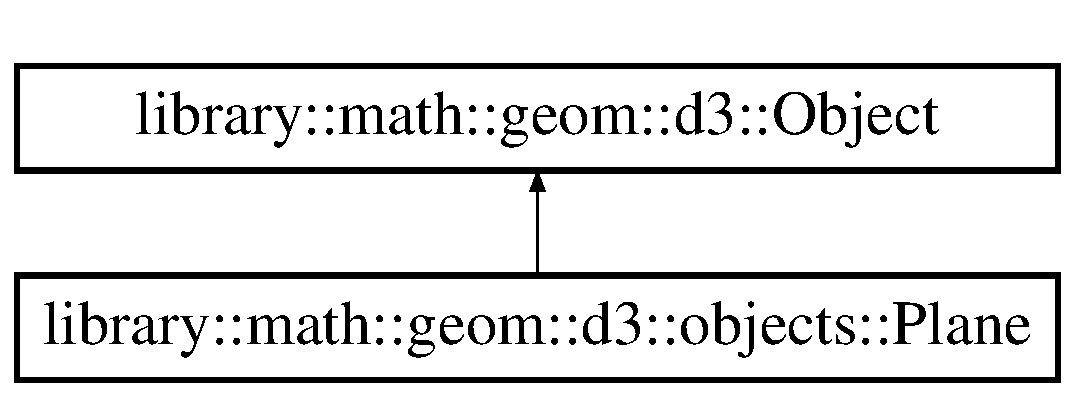
\includegraphics[height=2.000000cm]{classlibrary_1_1math_1_1geom_1_1d3_1_1objects_1_1_plane}
\end{center}
\end{figure}
\subsection*{Public Member Functions}
\begin{DoxyCompactItemize}
\item 
\hyperlink{classlibrary_1_1math_1_1geom_1_1d3_1_1objects_1_1_plane_a81fe78a983e2cb6ee6ad9bfabd22c3a4}{Plane} (const \hyperlink{classlibrary_1_1math_1_1geom_1_1d3_1_1objects_1_1_point}{Point} \&a\+Point, const Vector3d \&a\+Normal\+Vector)
\begin{DoxyCompactList}\small\item\em Constructor. \end{DoxyCompactList}\item 
virtual \hyperlink{classlibrary_1_1math_1_1geom_1_1d3_1_1objects_1_1_plane}{Plane} $\ast$ \hyperlink{classlibrary_1_1math_1_1geom_1_1d3_1_1objects_1_1_plane_a0b6a4ae7bef06f3995f8fd9d32a88870}{clone} () const override
\begin{DoxyCompactList}\small\item\em Clone plane. \end{DoxyCompactList}\item 
bool \hyperlink{classlibrary_1_1math_1_1geom_1_1d3_1_1objects_1_1_plane_a9391589825cac1db971b39452b38f8ea}{operator==} (const \hyperlink{classlibrary_1_1math_1_1geom_1_1d3_1_1objects_1_1_plane}{Plane} \&a\+Plane) const
\begin{DoxyCompactList}\small\item\em Equal to operator. \end{DoxyCompactList}\item 
bool \hyperlink{classlibrary_1_1math_1_1geom_1_1d3_1_1objects_1_1_plane_a5dfafb90b0da2cc239092ea6c655ec2a}{operator!=} (const \hyperlink{classlibrary_1_1math_1_1geom_1_1d3_1_1objects_1_1_plane}{Plane} \&a\+Plane) const
\begin{DoxyCompactList}\small\item\em Not equal to operator. \end{DoxyCompactList}\item 
virtual bool \hyperlink{classlibrary_1_1math_1_1geom_1_1d3_1_1objects_1_1_plane_aafbc8274c270be143b2fa3dc46459f17}{is\+Defined} () const override
\begin{DoxyCompactList}\small\item\em Check if plane is defined. \end{DoxyCompactList}\item 
bool \hyperlink{classlibrary_1_1math_1_1geom_1_1d3_1_1objects_1_1_plane_a7bb2f2a298461ee30c77ad653cfd195a}{contains} (const \hyperlink{classlibrary_1_1math_1_1geom_1_1d3_1_1objects_1_1_point}{Point} \&a\+Point) const
\begin{DoxyCompactList}\small\item\em Check if plane contains point. \end{DoxyCompactList}\item 
\hyperlink{classlibrary_1_1math_1_1geom_1_1d3_1_1objects_1_1_point}{Point} \hyperlink{classlibrary_1_1math_1_1geom_1_1d3_1_1objects_1_1_plane_a52f9167ca123019c4b303c19b696b886}{get\+Point} () const
\begin{DoxyCompactList}\small\item\em Get plane point. \end{DoxyCompactList}\item 
Vector3d \hyperlink{classlibrary_1_1math_1_1geom_1_1d3_1_1objects_1_1_plane_a9d34608a389d4c80dad6b6f58b82c0e4}{get\+Normal\+Vector} () const
\begin{DoxyCompactList}\small\item\em Get plane normal vector. \end{DoxyCompactList}\item 
virtual void \hyperlink{classlibrary_1_1math_1_1geom_1_1d3_1_1objects_1_1_plane_a2e43e82344b57898606f5c13ffc9dcc9}{print} (std\+::ostream \&an\+Output\+Stream, bool display\+Decorators=true) const override
\begin{DoxyCompactList}\small\item\em Print plane. \end{DoxyCompactList}\item 
virtual void \hyperlink{classlibrary_1_1math_1_1geom_1_1d3_1_1objects_1_1_plane_ab3474aef2e9f8dd4f9e86da017522487}{apply\+Transformation} (const \hyperlink{classlibrary_1_1math_1_1geom_1_1d3_1_1_transformation}{Transformation} \&a\+Transformation) override
\begin{DoxyCompactList}\small\item\em Apply transformation to plane. \end{DoxyCompactList}\end{DoxyCompactItemize}
\subsection*{Static Public Member Functions}
\begin{DoxyCompactItemize}
\item 
static \hyperlink{classlibrary_1_1math_1_1geom_1_1d3_1_1objects_1_1_plane}{Plane} \hyperlink{classlibrary_1_1math_1_1geom_1_1d3_1_1objects_1_1_plane_a582c0e5930dd4a458c557c866b0dae17}{Undefined} ()
\begin{DoxyCompactList}\small\item\em Constructs an undefined plane. \end{DoxyCompactList}\end{DoxyCompactItemize}


\subsection{Detailed Description}
\hyperlink{classlibrary_1_1math_1_1geom_1_1d3_1_1objects_1_1_plane}{Plane}. 

A plane is a flat, two-\/dimensional surface that extends infinitely far.

https\+://en.wikipedia.\+org/wiki/\+Plane\+\_\+(geometry) 

\subsection{Constructor \& Destructor Documentation}
\mbox{\Hypertarget{classlibrary_1_1math_1_1geom_1_1d3_1_1objects_1_1_plane_a81fe78a983e2cb6ee6ad9bfabd22c3a4}\label{classlibrary_1_1math_1_1geom_1_1d3_1_1objects_1_1_plane_a81fe78a983e2cb6ee6ad9bfabd22c3a4}} 
\index{library\+::math\+::geom\+::d3\+::objects\+::\+Plane@{library\+::math\+::geom\+::d3\+::objects\+::\+Plane}!Plane@{Plane}}
\index{Plane@{Plane}!library\+::math\+::geom\+::d3\+::objects\+::\+Plane@{library\+::math\+::geom\+::d3\+::objects\+::\+Plane}}
\subsubsection{\texorpdfstring{Plane()}{Plane()}}
{\footnotesize\ttfamily library\+::math\+::geom\+::d3\+::objects\+::\+Plane\+::\+Plane (\begin{DoxyParamCaption}\item[{const \hyperlink{classlibrary_1_1math_1_1geom_1_1d3_1_1objects_1_1_point}{Point} \&}]{a\+Point,  }\item[{const Vector3d \&}]{a\+Normal\+Vector }\end{DoxyParamCaption})}



Constructor. 


\begin{DoxyCode}
\hyperlink{classlibrary_1_1math_1_1geom_1_1d3_1_1objects_1_1_plane_a81fe78a983e2cb6ee6ad9bfabd22c3a4}{Plane} plane(\{ 0.0, 0.0, 0.0 \}, \{ 0.0, 0.0, 1.0 \}) ;
\end{DoxyCode}



\begin{DoxyParams}[1]{Parameters}
\mbox{\tt in}  & {\em a\+Point} & A point \\
\hline
\mbox{\tt in}  & {\em a\+Normal\+Vector} & A normal vector \\
\hline
\end{DoxyParams}


\subsection{Member Function Documentation}
\mbox{\Hypertarget{classlibrary_1_1math_1_1geom_1_1d3_1_1objects_1_1_plane_ab3474aef2e9f8dd4f9e86da017522487}\label{classlibrary_1_1math_1_1geom_1_1d3_1_1objects_1_1_plane_ab3474aef2e9f8dd4f9e86da017522487}} 
\index{library\+::math\+::geom\+::d3\+::objects\+::\+Plane@{library\+::math\+::geom\+::d3\+::objects\+::\+Plane}!apply\+Transformation@{apply\+Transformation}}
\index{apply\+Transformation@{apply\+Transformation}!library\+::math\+::geom\+::d3\+::objects\+::\+Plane@{library\+::math\+::geom\+::d3\+::objects\+::\+Plane}}
\subsubsection{\texorpdfstring{apply\+Transformation()}{applyTransformation()}}
{\footnotesize\ttfamily void library\+::math\+::geom\+::d3\+::objects\+::\+Plane\+::apply\+Transformation (\begin{DoxyParamCaption}\item[{const \hyperlink{classlibrary_1_1math_1_1geom_1_1d3_1_1_transformation}{Transformation} \&}]{a\+Transformation }\end{DoxyParamCaption})\hspace{0.3cm}{\ttfamily [override]}, {\ttfamily [virtual]}}



Apply transformation to plane. 


\begin{DoxyParams}[1]{Parameters}
\mbox{\tt in}  & {\em a\+Transformation} & A transformation \\
\hline
\end{DoxyParams}


Implements \hyperlink{classlibrary_1_1math_1_1geom_1_1d3_1_1_object_a5fc47b1ee5d9a28efc6010d3d1512470}{library\+::math\+::geom\+::d3\+::\+Object}.

\mbox{\Hypertarget{classlibrary_1_1math_1_1geom_1_1d3_1_1objects_1_1_plane_a0b6a4ae7bef06f3995f8fd9d32a88870}\label{classlibrary_1_1math_1_1geom_1_1d3_1_1objects_1_1_plane_a0b6a4ae7bef06f3995f8fd9d32a88870}} 
\index{library\+::math\+::geom\+::d3\+::objects\+::\+Plane@{library\+::math\+::geom\+::d3\+::objects\+::\+Plane}!clone@{clone}}
\index{clone@{clone}!library\+::math\+::geom\+::d3\+::objects\+::\+Plane@{library\+::math\+::geom\+::d3\+::objects\+::\+Plane}}
\subsubsection{\texorpdfstring{clone()}{clone()}}
{\footnotesize\ttfamily \hyperlink{classlibrary_1_1math_1_1geom_1_1d3_1_1objects_1_1_plane}{Plane} $\ast$ library\+::math\+::geom\+::d3\+::objects\+::\+Plane\+::clone (\begin{DoxyParamCaption}{ }\end{DoxyParamCaption}) const\hspace{0.3cm}{\ttfamily [override]}, {\ttfamily [virtual]}}



Clone plane. 

\begin{DoxyReturn}{Returns}
Pointer to cloned plane 
\end{DoxyReturn}


Implements \hyperlink{classlibrary_1_1math_1_1geom_1_1d3_1_1_object_a1a784c6b359e0eb97cd34fabc42f2f3f}{library\+::math\+::geom\+::d3\+::\+Object}.

\mbox{\Hypertarget{classlibrary_1_1math_1_1geom_1_1d3_1_1objects_1_1_plane_a7bb2f2a298461ee30c77ad653cfd195a}\label{classlibrary_1_1math_1_1geom_1_1d3_1_1objects_1_1_plane_a7bb2f2a298461ee30c77ad653cfd195a}} 
\index{library\+::math\+::geom\+::d3\+::objects\+::\+Plane@{library\+::math\+::geom\+::d3\+::objects\+::\+Plane}!contains@{contains}}
\index{contains@{contains}!library\+::math\+::geom\+::d3\+::objects\+::\+Plane@{library\+::math\+::geom\+::d3\+::objects\+::\+Plane}}
\subsubsection{\texorpdfstring{contains()}{contains()}}
{\footnotesize\ttfamily bool library\+::math\+::geom\+::d3\+::objects\+::\+Plane\+::contains (\begin{DoxyParamCaption}\item[{const \hyperlink{classlibrary_1_1math_1_1geom_1_1d3_1_1objects_1_1_point}{Point} \&}]{a\+Point }\end{DoxyParamCaption}) const}



Check if plane contains point. 


\begin{DoxyCode}
Point plane = ... ;
Point point = ... ;
plane.contains(point) ;
\end{DoxyCode}



\begin{DoxyParams}[1]{Parameters}
\mbox{\tt in}  & {\em a\+Point} & A point \\
\hline
\end{DoxyParams}
\begin{DoxyReturn}{Returns}
True if plane contains point 
\end{DoxyReturn}
\mbox{\Hypertarget{classlibrary_1_1math_1_1geom_1_1d3_1_1objects_1_1_plane_a9d34608a389d4c80dad6b6f58b82c0e4}\label{classlibrary_1_1math_1_1geom_1_1d3_1_1objects_1_1_plane_a9d34608a389d4c80dad6b6f58b82c0e4}} 
\index{library\+::math\+::geom\+::d3\+::objects\+::\+Plane@{library\+::math\+::geom\+::d3\+::objects\+::\+Plane}!get\+Normal\+Vector@{get\+Normal\+Vector}}
\index{get\+Normal\+Vector@{get\+Normal\+Vector}!library\+::math\+::geom\+::d3\+::objects\+::\+Plane@{library\+::math\+::geom\+::d3\+::objects\+::\+Plane}}
\subsubsection{\texorpdfstring{get\+Normal\+Vector()}{getNormalVector()}}
{\footnotesize\ttfamily Vector3d library\+::math\+::geom\+::d3\+::objects\+::\+Plane\+::get\+Normal\+Vector (\begin{DoxyParamCaption}{ }\end{DoxyParamCaption}) const}



Get plane normal vector. 


\begin{DoxyCode}
\hyperlink{classlibrary_1_1math_1_1geom_1_1d3_1_1objects_1_1_plane_a81fe78a983e2cb6ee6ad9bfabd22c3a4}{Plane}(\{ 0.0, 0.0, 0.0 \}, \{ 0.0, 0.0, 1.0 \}).\hyperlink{classlibrary_1_1math_1_1geom_1_1d3_1_1objects_1_1_plane_a9d34608a389d4c80dad6b6f58b82c0e4}{getNormalVector}() ; \textcolor{comment}{// [0.0, 0.0, 1.0]}
\end{DoxyCode}


\begin{DoxyReturn}{Returns}
\hyperlink{classlibrary_1_1math_1_1geom_1_1d3_1_1objects_1_1_plane}{Plane} normal vector 
\end{DoxyReturn}
\mbox{\Hypertarget{classlibrary_1_1math_1_1geom_1_1d3_1_1objects_1_1_plane_a52f9167ca123019c4b303c19b696b886}\label{classlibrary_1_1math_1_1geom_1_1d3_1_1objects_1_1_plane_a52f9167ca123019c4b303c19b696b886}} 
\index{library\+::math\+::geom\+::d3\+::objects\+::\+Plane@{library\+::math\+::geom\+::d3\+::objects\+::\+Plane}!get\+Point@{get\+Point}}
\index{get\+Point@{get\+Point}!library\+::math\+::geom\+::d3\+::objects\+::\+Plane@{library\+::math\+::geom\+::d3\+::objects\+::\+Plane}}
\subsubsection{\texorpdfstring{get\+Point()}{getPoint()}}
{\footnotesize\ttfamily \hyperlink{classlibrary_1_1math_1_1geom_1_1d3_1_1objects_1_1_point}{Point} library\+::math\+::geom\+::d3\+::objects\+::\+Plane\+::get\+Point (\begin{DoxyParamCaption}{ }\end{DoxyParamCaption}) const}



Get plane point. 


\begin{DoxyCode}
\hyperlink{classlibrary_1_1math_1_1geom_1_1d3_1_1objects_1_1_plane_a81fe78a983e2cb6ee6ad9bfabd22c3a4}{Plane}(\{ 0.0, 0.0, 0.0 \}, \{ 0.0, 0.0, 1.0 \}).\hyperlink{classlibrary_1_1math_1_1geom_1_1d3_1_1objects_1_1_plane_a52f9167ca123019c4b303c19b696b886}{getPoint}() ; \textcolor{comment}{// [0.0, 0.0, 0.0]}
\end{DoxyCode}


\begin{DoxyReturn}{Returns}
\hyperlink{classlibrary_1_1math_1_1geom_1_1d3_1_1objects_1_1_plane}{Plane} point 
\end{DoxyReturn}
\mbox{\Hypertarget{classlibrary_1_1math_1_1geom_1_1d3_1_1objects_1_1_plane_aafbc8274c270be143b2fa3dc46459f17}\label{classlibrary_1_1math_1_1geom_1_1d3_1_1objects_1_1_plane_aafbc8274c270be143b2fa3dc46459f17}} 
\index{library\+::math\+::geom\+::d3\+::objects\+::\+Plane@{library\+::math\+::geom\+::d3\+::objects\+::\+Plane}!is\+Defined@{is\+Defined}}
\index{is\+Defined@{is\+Defined}!library\+::math\+::geom\+::d3\+::objects\+::\+Plane@{library\+::math\+::geom\+::d3\+::objects\+::\+Plane}}
\subsubsection{\texorpdfstring{is\+Defined()}{isDefined()}}
{\footnotesize\ttfamily bool library\+::math\+::geom\+::d3\+::objects\+::\+Plane\+::is\+Defined (\begin{DoxyParamCaption}{ }\end{DoxyParamCaption}) const\hspace{0.3cm}{\ttfamily [override]}, {\ttfamily [virtual]}}



Check if plane is defined. 


\begin{DoxyCode}
\hyperlink{classlibrary_1_1math_1_1geom_1_1d3_1_1objects_1_1_plane_a81fe78a983e2cb6ee6ad9bfabd22c3a4}{Plane}(\{ 0.0, 0.0, 0.0 \}, \{ 0.0, 0.0, 1.0 \}).\hyperlink{classlibrary_1_1math_1_1geom_1_1d3_1_1objects_1_1_plane_aafbc8274c270be143b2fa3dc46459f17}{isDefined}() ; \textcolor{comment}{// True}
\end{DoxyCode}


\begin{DoxyReturn}{Returns}
True if plane is defined 
\end{DoxyReturn}


Implements \hyperlink{classlibrary_1_1math_1_1geom_1_1d3_1_1_object_a2216442e322f0c3ca5f01a4efa22baf7}{library\+::math\+::geom\+::d3\+::\+Object}.

\mbox{\Hypertarget{classlibrary_1_1math_1_1geom_1_1d3_1_1objects_1_1_plane_a5dfafb90b0da2cc239092ea6c655ec2a}\label{classlibrary_1_1math_1_1geom_1_1d3_1_1objects_1_1_plane_a5dfafb90b0da2cc239092ea6c655ec2a}} 
\index{library\+::math\+::geom\+::d3\+::objects\+::\+Plane@{library\+::math\+::geom\+::d3\+::objects\+::\+Plane}!operator"!=@{operator"!=}}
\index{operator"!=@{operator"!=}!library\+::math\+::geom\+::d3\+::objects\+::\+Plane@{library\+::math\+::geom\+::d3\+::objects\+::\+Plane}}
\subsubsection{\texorpdfstring{operator"!=()}{operator!=()}}
{\footnotesize\ttfamily bool library\+::math\+::geom\+::d3\+::objects\+::\+Plane\+::operator!= (\begin{DoxyParamCaption}\item[{const \hyperlink{classlibrary_1_1math_1_1geom_1_1d3_1_1objects_1_1_plane}{Plane} \&}]{a\+Plane }\end{DoxyParamCaption}) const}



Not equal to operator. 


\begin{DoxyCode}
\hyperlink{classlibrary_1_1math_1_1geom_1_1d3_1_1objects_1_1_plane_a81fe78a983e2cb6ee6ad9bfabd22c3a4}{Plane}(\{ 0.0, 0.0, 0.0 \}, \{ 0.0, 0.0, 1.0 \}) != \hyperlink{classlibrary_1_1math_1_1geom_1_1d3_1_1objects_1_1_plane_a81fe78a983e2cb6ee6ad9bfabd22c3a4}{Plane}(\{ 0.0, 0.0, 1.0 \}, \{ 0.0, 0.0, 1.0 \}) ; \textcolor{comment}{//
       True}
\end{DoxyCode}



\begin{DoxyParams}[1]{Parameters}
\mbox{\tt in}  & {\em a\+Plane} & A plane \\
\hline
\end{DoxyParams}
\begin{DoxyReturn}{Returns}
True if planes not are equal 
\end{DoxyReturn}
\mbox{\Hypertarget{classlibrary_1_1math_1_1geom_1_1d3_1_1objects_1_1_plane_a9391589825cac1db971b39452b38f8ea}\label{classlibrary_1_1math_1_1geom_1_1d3_1_1objects_1_1_plane_a9391589825cac1db971b39452b38f8ea}} 
\index{library\+::math\+::geom\+::d3\+::objects\+::\+Plane@{library\+::math\+::geom\+::d3\+::objects\+::\+Plane}!operator==@{operator==}}
\index{operator==@{operator==}!library\+::math\+::geom\+::d3\+::objects\+::\+Plane@{library\+::math\+::geom\+::d3\+::objects\+::\+Plane}}
\subsubsection{\texorpdfstring{operator==()}{operator==()}}
{\footnotesize\ttfamily bool library\+::math\+::geom\+::d3\+::objects\+::\+Plane\+::operator== (\begin{DoxyParamCaption}\item[{const \hyperlink{classlibrary_1_1math_1_1geom_1_1d3_1_1objects_1_1_plane}{Plane} \&}]{a\+Plane }\end{DoxyParamCaption}) const}



Equal to operator. 


\begin{DoxyCode}
\hyperlink{classlibrary_1_1math_1_1geom_1_1d3_1_1objects_1_1_plane_a81fe78a983e2cb6ee6ad9bfabd22c3a4}{Plane}(\{ 0.0, 0.0, 0.0 \}, \{ 0.0, 0.0, 1.0 \}) == \hyperlink{classlibrary_1_1math_1_1geom_1_1d3_1_1objects_1_1_plane_a81fe78a983e2cb6ee6ad9bfabd22c3a4}{Plane}(\{ 0.0, 0.0, 0.0 \}, \{ 0.0, 0.0, 1.0 \}) ; \textcolor{comment}{//
       True}
\end{DoxyCode}



\begin{DoxyParams}[1]{Parameters}
\mbox{\tt in}  & {\em a\+Plane} & A plane \\
\hline
\end{DoxyParams}
\begin{DoxyReturn}{Returns}
True if planes are equal 
\end{DoxyReturn}
\mbox{\Hypertarget{classlibrary_1_1math_1_1geom_1_1d3_1_1objects_1_1_plane_a2e43e82344b57898606f5c13ffc9dcc9}\label{classlibrary_1_1math_1_1geom_1_1d3_1_1objects_1_1_plane_a2e43e82344b57898606f5c13ffc9dcc9}} 
\index{library\+::math\+::geom\+::d3\+::objects\+::\+Plane@{library\+::math\+::geom\+::d3\+::objects\+::\+Plane}!print@{print}}
\index{print@{print}!library\+::math\+::geom\+::d3\+::objects\+::\+Plane@{library\+::math\+::geom\+::d3\+::objects\+::\+Plane}}
\subsubsection{\texorpdfstring{print()}{print()}}
{\footnotesize\ttfamily void library\+::math\+::geom\+::d3\+::objects\+::\+Plane\+::print (\begin{DoxyParamCaption}\item[{std\+::ostream \&}]{an\+Output\+Stream,  }\item[{bool}]{display\+Decorators = {\ttfamily true} }\end{DoxyParamCaption}) const\hspace{0.3cm}{\ttfamily [override]}, {\ttfamily [virtual]}}



Print plane. 


\begin{DoxyParams}[1]{Parameters}
\mbox{\tt in}  & {\em an\+Output\+Stream} & An output stream \\
\hline
\mbox{\tt in}  & {\em (optional)} & display\+Decorators If true, display decorators \\
\hline
\end{DoxyParams}


Implements \hyperlink{classlibrary_1_1math_1_1geom_1_1d3_1_1_object_aa166f4ce4d116a248f0fc861c75012ca}{library\+::math\+::geom\+::d3\+::\+Object}.

\mbox{\Hypertarget{classlibrary_1_1math_1_1geom_1_1d3_1_1objects_1_1_plane_a582c0e5930dd4a458c557c866b0dae17}\label{classlibrary_1_1math_1_1geom_1_1d3_1_1objects_1_1_plane_a582c0e5930dd4a458c557c866b0dae17}} 
\index{library\+::math\+::geom\+::d3\+::objects\+::\+Plane@{library\+::math\+::geom\+::d3\+::objects\+::\+Plane}!Undefined@{Undefined}}
\index{Undefined@{Undefined}!library\+::math\+::geom\+::d3\+::objects\+::\+Plane@{library\+::math\+::geom\+::d3\+::objects\+::\+Plane}}
\subsubsection{\texorpdfstring{Undefined()}{Undefined()}}
{\footnotesize\ttfamily \hyperlink{classlibrary_1_1math_1_1geom_1_1d3_1_1objects_1_1_plane}{Plane} library\+::math\+::geom\+::d3\+::objects\+::\+Plane\+::\+Undefined (\begin{DoxyParamCaption}{ }\end{DoxyParamCaption})\hspace{0.3cm}{\ttfamily [static]}}



Constructs an undefined plane. 


\begin{DoxyCode}
\hyperlink{classlibrary_1_1math_1_1geom_1_1d3_1_1objects_1_1_plane_a81fe78a983e2cb6ee6ad9bfabd22c3a4}{Plane} plane = \hyperlink{classlibrary_1_1math_1_1geom_1_1d3_1_1objects_1_1_plane_a582c0e5930dd4a458c557c866b0dae17}{Plane::Undefined}() ; \textcolor{comment}{// Undefined}
\end{DoxyCode}


\begin{DoxyReturn}{Returns}
Undefined plane 
\end{DoxyReturn}


The documentation for this class was generated from the following files\+:\begin{DoxyCompactItemize}
\item 
include/\+Library/\+Mathematics/\+Geometry/3\+D/\+Objects/\hyperlink{_plane_8hpp}{Plane.\+hpp}\item 
src/\+Library/\+Mathematics/\+Geometry/3\+D/\+Objects/\hyperlink{_plane_8cpp}{Plane.\+cpp}\end{DoxyCompactItemize}

\hypertarget{classlibrary_1_1math_1_1geom_1_1d3_1_1objects_1_1_point}{}\section{library\+:\+:math\+:\+:geom\+:\+:d3\+:\+:objects\+:\+:Point Class Reference}
\label{classlibrary_1_1math_1_1geom_1_1d3_1_1objects_1_1_point}\index{library\+::math\+::geom\+::d3\+::objects\+::\+Point@{library\+::math\+::geom\+::d3\+::objects\+::\+Point}}


\hyperlink{classlibrary_1_1math_1_1geom_1_1d3_1_1objects_1_1_point}{Point}.  




{\ttfamily \#include $<$Point.\+hpp$>$}

Inheritance diagram for library\+:\+:math\+:\+:geom\+:\+:d3\+:\+:objects\+:\+:Point\+:\begin{figure}[H]
\begin{center}
\leavevmode
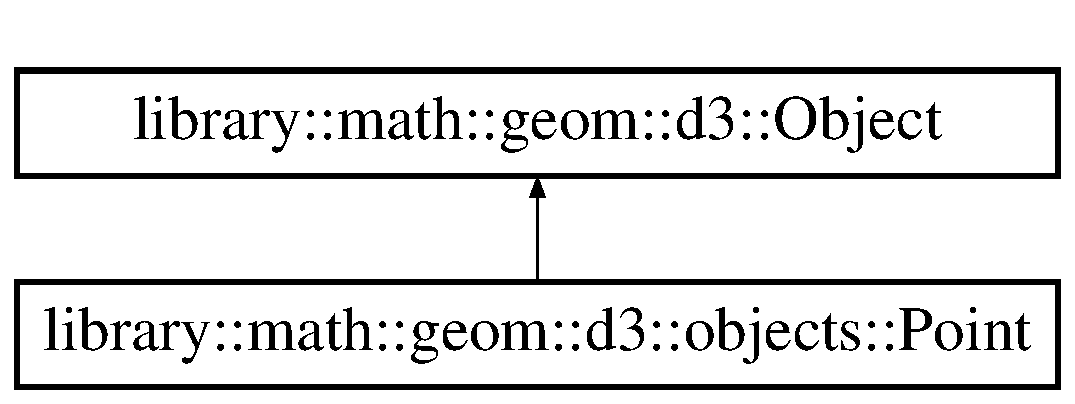
\includegraphics[height=2.000000cm]{classlibrary_1_1math_1_1geom_1_1d3_1_1objects_1_1_point}
\end{center}
\end{figure}
\subsection*{Public Member Functions}
\begin{DoxyCompactItemize}
\item 
\hyperlink{classlibrary_1_1math_1_1geom_1_1d3_1_1objects_1_1_point_a617e690ab6091af3de729cee337e309e}{Point} (const Real \&a\+First\+Coordinate, const Real \&a\+Second\+Coordinate, const Real \&a\+Third\+Coordinate)
\begin{DoxyCompactList}\small\item\em Constructor. \end{DoxyCompactList}\item 
\hyperlink{classlibrary_1_1math_1_1geom_1_1d3_1_1objects_1_1_point_aa247b14e8237860aafa86bee66f074e0}{Point} (const Vector3d \&a\+Vector)
\begin{DoxyCompactList}\small\item\em Constructor. \end{DoxyCompactList}\item 
virtual \hyperlink{classlibrary_1_1math_1_1geom_1_1d3_1_1objects_1_1_point}{Point} $\ast$ \hyperlink{classlibrary_1_1math_1_1geom_1_1d3_1_1objects_1_1_point_a32aa1e233c6ac5341605961f6bf0f210}{clone} () const override
\begin{DoxyCompactList}\small\item\em Clone point. \end{DoxyCompactList}\item 
bool \hyperlink{classlibrary_1_1math_1_1geom_1_1d3_1_1objects_1_1_point_a0e89a102cf4e3f77b26e0bf234a69075}{operator==} (const \hyperlink{classlibrary_1_1math_1_1geom_1_1d3_1_1objects_1_1_point}{Point} \&a\+Point) const
\begin{DoxyCompactList}\small\item\em Equal to operator. \end{DoxyCompactList}\item 
bool \hyperlink{classlibrary_1_1math_1_1geom_1_1d3_1_1objects_1_1_point_abf144133b487834091866a71116ce31a}{operator!=} (const \hyperlink{classlibrary_1_1math_1_1geom_1_1d3_1_1objects_1_1_point}{Point} \&a\+Point) const
\begin{DoxyCompactList}\small\item\em Not equal to operator. \end{DoxyCompactList}\item 
virtual bool \hyperlink{classlibrary_1_1math_1_1geom_1_1d3_1_1objects_1_1_point_a9874289efeb457ada4b32d7eb1e012f6}{is\+Defined} () const override
\begin{DoxyCompactList}\small\item\em Addition operator\+: translate point along vector. \end{DoxyCompactList}\item 
bool \hyperlink{classlibrary_1_1math_1_1geom_1_1d3_1_1objects_1_1_point_a0bcdce172502509f9b9d4e5b3fc75a69}{is\+Near} (const \hyperlink{classlibrary_1_1math_1_1geom_1_1d3_1_1objects_1_1_point}{Point} \&a\+Point, const Real \&a\+Tolerance) const
\begin{DoxyCompactList}\small\item\em Check if point is near another point. \end{DoxyCompactList}\item 
Real \hyperlink{classlibrary_1_1math_1_1geom_1_1d3_1_1objects_1_1_point_a0108b685599f2684837d2898250c5a36}{distance\+To} (const \hyperlink{classlibrary_1_1math_1_1geom_1_1d3_1_1objects_1_1_point}{Point} \&a\+Point) const
\begin{DoxyCompactList}\small\item\em Get distance to another point. \end{DoxyCompactList}\item 
virtual void \hyperlink{classlibrary_1_1math_1_1geom_1_1d3_1_1objects_1_1_point_a76847422ebfcc28388d1b0427a5cb1de}{print} (std\+::ostream \&an\+Output\+Stream, bool display\+Decorators=true) const override
\begin{DoxyCompactList}\small\item\em Print point. \end{DoxyCompactList}\item 
virtual void \hyperlink{classlibrary_1_1math_1_1geom_1_1d3_1_1objects_1_1_point_ad2052f6ef5df88b75cae09c58a678f95}{apply\+Transformation} (const \hyperlink{classlibrary_1_1math_1_1geom_1_1d3_1_1_transformation}{Transformation} \&a\+Transformation) override
\begin{DoxyCompactList}\small\item\em Apply transformation to point. \end{DoxyCompactList}\end{DoxyCompactItemize}
\subsection*{Static Public Member Functions}
\begin{DoxyCompactItemize}
\item 
static \hyperlink{classlibrary_1_1math_1_1geom_1_1d3_1_1objects_1_1_point}{Point} \hyperlink{classlibrary_1_1math_1_1geom_1_1d3_1_1objects_1_1_point_a7c4c9c71f9b29b85925d8a7ed4943501}{Undefined} ()
\begin{DoxyCompactList}\small\item\em Constructs an undefined point. \end{DoxyCompactList}\item 
static \hyperlink{classlibrary_1_1math_1_1geom_1_1d3_1_1objects_1_1_point}{Point} \hyperlink{classlibrary_1_1math_1_1geom_1_1d3_1_1objects_1_1_point_ab2a38e285c562e50bf350272c083986f}{Origin} ()
\begin{DoxyCompactList}\small\item\em Constructs a point at origin. \end{DoxyCompactList}\end{DoxyCompactItemize}


\subsection{Detailed Description}
\hyperlink{classlibrary_1_1math_1_1geom_1_1d3_1_1objects_1_1_point}{Point}. 

https\+://en.wikipedia.\+org/wiki/\+Point\+\_\+(geometry) 

\subsection{Constructor \& Destructor Documentation}
\mbox{\Hypertarget{classlibrary_1_1math_1_1geom_1_1d3_1_1objects_1_1_point_a617e690ab6091af3de729cee337e309e}\label{classlibrary_1_1math_1_1geom_1_1d3_1_1objects_1_1_point_a617e690ab6091af3de729cee337e309e}} 
\index{library\+::math\+::geom\+::d3\+::objects\+::\+Point@{library\+::math\+::geom\+::d3\+::objects\+::\+Point}!Point@{Point}}
\index{Point@{Point}!library\+::math\+::geom\+::d3\+::objects\+::\+Point@{library\+::math\+::geom\+::d3\+::objects\+::\+Point}}
\subsubsection{\texorpdfstring{Point()}{Point()}\hspace{0.1cm}{\footnotesize\ttfamily [1/2]}}
{\footnotesize\ttfamily library\+::math\+::geom\+::d3\+::objects\+::\+Point\+::\+Point (\begin{DoxyParamCaption}\item[{const Real \&}]{a\+First\+Coordinate,  }\item[{const Real \&}]{a\+Second\+Coordinate,  }\item[{const Real \&}]{a\+Third\+Coordinate }\end{DoxyParamCaption})}



Constructor. 


\begin{DoxyCode}
\hyperlink{classlibrary_1_1math_1_1geom_1_1d3_1_1objects_1_1_point_a617e690ab6091af3de729cee337e309e}{Point} point(0.0, 0.0, 0.0) ;
\end{DoxyCode}



\begin{DoxyParams}[1]{Parameters}
\mbox{\tt in}  & {\em a\+First\+Coordinate} & A first coordinate \\
\hline
\mbox{\tt in}  & {\em a\+Second\+Coordinate} & A second coordinate \\
\hline
\mbox{\tt in}  & {\em a\+Third\+Coordinate} & A third coordinate \\
\hline
\end{DoxyParams}
\mbox{\Hypertarget{classlibrary_1_1math_1_1geom_1_1d3_1_1objects_1_1_point_aa247b14e8237860aafa86bee66f074e0}\label{classlibrary_1_1math_1_1geom_1_1d3_1_1objects_1_1_point_aa247b14e8237860aafa86bee66f074e0}} 
\index{library\+::math\+::geom\+::d3\+::objects\+::\+Point@{library\+::math\+::geom\+::d3\+::objects\+::\+Point}!Point@{Point}}
\index{Point@{Point}!library\+::math\+::geom\+::d3\+::objects\+::\+Point@{library\+::math\+::geom\+::d3\+::objects\+::\+Point}}
\subsubsection{\texorpdfstring{Point()}{Point()}\hspace{0.1cm}{\footnotesize\ttfamily [2/2]}}
{\footnotesize\ttfamily library\+::math\+::geom\+::d3\+::objects\+::\+Point\+::\+Point (\begin{DoxyParamCaption}\item[{const Vector3d \&}]{a\+Vector }\end{DoxyParamCaption})}



Constructor. 


\begin{DoxyCode}
\hyperlink{classlibrary_1_1math_1_1geom_1_1d3_1_1objects_1_1_point_a617e690ab6091af3de729cee337e309e}{Point} point(\{ 0.0, 0.0, 0.0 \}) ;
\end{DoxyCode}



\begin{DoxyParams}[1]{Parameters}
\mbox{\tt in}  & {\em a\+Vector} & A position vector \\
\hline
\end{DoxyParams}


\subsection{Member Function Documentation}
\mbox{\Hypertarget{classlibrary_1_1math_1_1geom_1_1d3_1_1objects_1_1_point_ad2052f6ef5df88b75cae09c58a678f95}\label{classlibrary_1_1math_1_1geom_1_1d3_1_1objects_1_1_point_ad2052f6ef5df88b75cae09c58a678f95}} 
\index{library\+::math\+::geom\+::d3\+::objects\+::\+Point@{library\+::math\+::geom\+::d3\+::objects\+::\+Point}!apply\+Transformation@{apply\+Transformation}}
\index{apply\+Transformation@{apply\+Transformation}!library\+::math\+::geom\+::d3\+::objects\+::\+Point@{library\+::math\+::geom\+::d3\+::objects\+::\+Point}}
\subsubsection{\texorpdfstring{apply\+Transformation()}{applyTransformation()}}
{\footnotesize\ttfamily void library\+::math\+::geom\+::d3\+::objects\+::\+Point\+::apply\+Transformation (\begin{DoxyParamCaption}\item[{const \hyperlink{classlibrary_1_1math_1_1geom_1_1d3_1_1_transformation}{Transformation} \&}]{a\+Transformation }\end{DoxyParamCaption})\hspace{0.3cm}{\ttfamily [override]}, {\ttfamily [virtual]}}



Apply transformation to point. 


\begin{DoxyParams}[1]{Parameters}
\mbox{\tt in}  & {\em a\+Transformation} & A transformation \\
\hline
\end{DoxyParams}


Implements \hyperlink{classlibrary_1_1math_1_1geom_1_1d3_1_1_object_a5fc47b1ee5d9a28efc6010d3d1512470}{library\+::math\+::geom\+::d3\+::\+Object}.

\mbox{\Hypertarget{classlibrary_1_1math_1_1geom_1_1d3_1_1objects_1_1_point_a32aa1e233c6ac5341605961f6bf0f210}\label{classlibrary_1_1math_1_1geom_1_1d3_1_1objects_1_1_point_a32aa1e233c6ac5341605961f6bf0f210}} 
\index{library\+::math\+::geom\+::d3\+::objects\+::\+Point@{library\+::math\+::geom\+::d3\+::objects\+::\+Point}!clone@{clone}}
\index{clone@{clone}!library\+::math\+::geom\+::d3\+::objects\+::\+Point@{library\+::math\+::geom\+::d3\+::objects\+::\+Point}}
\subsubsection{\texorpdfstring{clone()}{clone()}}
{\footnotesize\ttfamily \hyperlink{classlibrary_1_1math_1_1geom_1_1d3_1_1objects_1_1_point}{Point} $\ast$ library\+::math\+::geom\+::d3\+::objects\+::\+Point\+::clone (\begin{DoxyParamCaption}{ }\end{DoxyParamCaption}) const\hspace{0.3cm}{\ttfamily [override]}, {\ttfamily [virtual]}}



Clone point. 

\begin{DoxyReturn}{Returns}
Pointer to cloned point 
\end{DoxyReturn}


Implements \hyperlink{classlibrary_1_1math_1_1geom_1_1d3_1_1_object_a1a784c6b359e0eb97cd34fabc42f2f3f}{library\+::math\+::geom\+::d3\+::\+Object}.

\mbox{\Hypertarget{classlibrary_1_1math_1_1geom_1_1d3_1_1objects_1_1_point_a0108b685599f2684837d2898250c5a36}\label{classlibrary_1_1math_1_1geom_1_1d3_1_1objects_1_1_point_a0108b685599f2684837d2898250c5a36}} 
\index{library\+::math\+::geom\+::d3\+::objects\+::\+Point@{library\+::math\+::geom\+::d3\+::objects\+::\+Point}!distance\+To@{distance\+To}}
\index{distance\+To@{distance\+To}!library\+::math\+::geom\+::d3\+::objects\+::\+Point@{library\+::math\+::geom\+::d3\+::objects\+::\+Point}}
\subsubsection{\texorpdfstring{distance\+To()}{distanceTo()}}
{\footnotesize\ttfamily Real library\+::math\+::geom\+::d3\+::objects\+::\+Point\+::distance\+To (\begin{DoxyParamCaption}\item[{const \hyperlink{classlibrary_1_1math_1_1geom_1_1d3_1_1objects_1_1_point}{Point} \&}]{a\+Point }\end{DoxyParamCaption}) const}



Get distance to another point. 


\begin{DoxyParams}[1]{Parameters}
\mbox{\tt in}  & {\em a\+Point} & A point \\
\hline
\end{DoxyParams}
\begin{DoxyReturn}{Returns}
Distance to point 
\end{DoxyReturn}
\mbox{\Hypertarget{classlibrary_1_1math_1_1geom_1_1d3_1_1objects_1_1_point_a9874289efeb457ada4b32d7eb1e012f6}\label{classlibrary_1_1math_1_1geom_1_1d3_1_1objects_1_1_point_a9874289efeb457ada4b32d7eb1e012f6}} 
\index{library\+::math\+::geom\+::d3\+::objects\+::\+Point@{library\+::math\+::geom\+::d3\+::objects\+::\+Point}!is\+Defined@{is\+Defined}}
\index{is\+Defined@{is\+Defined}!library\+::math\+::geom\+::d3\+::objects\+::\+Point@{library\+::math\+::geom\+::d3\+::objects\+::\+Point}}
\subsubsection{\texorpdfstring{is\+Defined()}{isDefined()}}
{\footnotesize\ttfamily bool library\+::math\+::geom\+::d3\+::objects\+::\+Point\+::is\+Defined (\begin{DoxyParamCaption}{ }\end{DoxyParamCaption}) const\hspace{0.3cm}{\ttfamily [override]}, {\ttfamily [virtual]}}



Addition operator\+: translate point along vector. 


\begin{DoxyCode}
                        \hyperlink{classlibrary_1_1math_1_1geom_1_1d3_1_1objects_1_1_point_a617e690ab6091af3de729cee337e309e}{Point}(0.0, 0.0, 0.0) + \hyperlink{namespacelibrary_1_1math_1_1obj_a977e84e9bf317a4e7dd9d6d671d6da2f}{Vector3d}(0.0, 0.0, 1.0) ; \textcolor{comment}{// [0.0, 0.0, 1.0]}
    @encode
   
    @param              [in] aVector A translation vector
    @\textcolor{keywordflow}{return}             A point

\hyperlink{classlibrary_1_1math_1_1geom_1_1d3_1_1objects_1_1_point_a617e690ab6091af3de729cee337e309e}{Point}                   operator +                                  (   \textcolor{keyword}{const}   
      \hyperlink{namespacelibrary_1_1math_1_1obj_a977e84e9bf317a4e7dd9d6d671d6da2f}{Vector3d}&                   aVector                                     ) \textcolor{keyword}{const} ;

    @brief              Subtraction \textcolor{keyword}{operator}: translate point along opposite vector
   
    @code
                        \hyperlink{classlibrary_1_1math_1_1geom_1_1d3_1_1objects_1_1_point_a617e690ab6091af3de729cee337e309e}{Point}(0.0, 0.0, 1.0) - \hyperlink{namespacelibrary_1_1math_1_1obj_a977e84e9bf317a4e7dd9d6d671d6da2f}{Vector3d}(0.0, 0.0, 1.0) ; \textcolor{comment}{// [0.0, 0.0, 0.0]}
    @encode
   
    @param              [in] aVector A translation vector
    @\textcolor{keywordflow}{return}             A point

\hyperlink{classlibrary_1_1math_1_1geom_1_1d3_1_1objects_1_1_point_a617e690ab6091af3de729cee337e309e}{Point}                   operator -                                  (   \textcolor{keyword}{const}   
      \hyperlink{namespacelibrary_1_1math_1_1obj_a977e84e9bf317a4e7dd9d6d671d6da2f}{Vector3d}&                   aVector                                     ) \textcolor{keyword}{const} ;

    @brief              Subtraction \textcolor{keyword}{operator}: \textcolor{keyword}{get} translation vector between two points
   
    @code
                        \hyperlink{classlibrary_1_1math_1_1geom_1_1d3_1_1objects_1_1_point_a617e690ab6091af3de729cee337e309e}{Point}(0.0, 0.0, 1.0) - \hyperlink{classlibrary_1_1math_1_1geom_1_1d3_1_1objects_1_1_point_a617e690ab6091af3de729cee337e309e}{Point}(0.0, 0.0, 0.0)  ; \textcolor{comment}{// [0.0, 0.0, 1.0]}
    @encode
   
    @param              [in] aPoint A point
    @\textcolor{keywordflow}{return}             A translation vector

\hyperlink{namespacelibrary_1_1math_1_1obj_a977e84e9bf317a4e7dd9d6d671d6da2f}{Vector3d}                operator -                                  (   \textcolor{keyword}{const}   
      \hyperlink{classlibrary_1_1math_1_1geom_1_1d3_1_1objects_1_1_point_a617e690ab6091af3de729cee337e309e}{Point}&                      aPoint                                      ) \textcolor{keyword}{const} ;

    @brief              Check \textcolor{keywordflow}{if} point is defined
   
    @code
                        \hyperlink{classlibrary_1_1math_1_1geom_1_1d3_1_1objects_1_1_point_a617e690ab6091af3de729cee337e309e}{Point}(0.0, 0.0, 0.0).isDefined() ; \textcolor{comment}{// True}
\end{DoxyCode}


\begin{DoxyReturn}{Returns}
True if point is defined 
\end{DoxyReturn}


Implements \hyperlink{classlibrary_1_1math_1_1geom_1_1d3_1_1_object_a2216442e322f0c3ca5f01a4efa22baf7}{library\+::math\+::geom\+::d3\+::\+Object}.

\mbox{\Hypertarget{classlibrary_1_1math_1_1geom_1_1d3_1_1objects_1_1_point_a0bcdce172502509f9b9d4e5b3fc75a69}\label{classlibrary_1_1math_1_1geom_1_1d3_1_1objects_1_1_point_a0bcdce172502509f9b9d4e5b3fc75a69}} 
\index{library\+::math\+::geom\+::d3\+::objects\+::\+Point@{library\+::math\+::geom\+::d3\+::objects\+::\+Point}!is\+Near@{is\+Near}}
\index{is\+Near@{is\+Near}!library\+::math\+::geom\+::d3\+::objects\+::\+Point@{library\+::math\+::geom\+::d3\+::objects\+::\+Point}}
\subsubsection{\texorpdfstring{is\+Near()}{isNear()}}
{\footnotesize\ttfamily bool library\+::math\+::geom\+::d3\+::objects\+::\+Point\+::is\+Near (\begin{DoxyParamCaption}\item[{const \hyperlink{classlibrary_1_1math_1_1geom_1_1d3_1_1objects_1_1_point}{Point} \&}]{a\+Point,  }\item[{const Real \&}]{a\+Tolerance }\end{DoxyParamCaption}) const}



Check if point is near another point. 


\begin{DoxyCode}
\hyperlink{classlibrary_1_1math_1_1geom_1_1d3_1_1objects_1_1_point_a617e690ab6091af3de729cee337e309e}{Point}(0.0, 0.0, 0.0).isNear(\hyperlink{classlibrary_1_1math_1_1geom_1_1d3_1_1objects_1_1_point_a617e690ab6091af3de729cee337e309e}{Point}(0.0, 0.0, 0.0), 1e-15) ; \textcolor{comment}{// True}
\end{DoxyCode}



\begin{DoxyParams}[1]{Parameters}
\mbox{\tt in}  & {\em a\+Point} & A point \\
\hline
\mbox{\tt in}  & {\em a\+Tolerance} & A tolerance \\
\hline
\end{DoxyParams}
\begin{DoxyReturn}{Returns}
True if point is near another point 
\end{DoxyReturn}
\mbox{\Hypertarget{classlibrary_1_1math_1_1geom_1_1d3_1_1objects_1_1_point_abf144133b487834091866a71116ce31a}\label{classlibrary_1_1math_1_1geom_1_1d3_1_1objects_1_1_point_abf144133b487834091866a71116ce31a}} 
\index{library\+::math\+::geom\+::d3\+::objects\+::\+Point@{library\+::math\+::geom\+::d3\+::objects\+::\+Point}!operator"!=@{operator"!=}}
\index{operator"!=@{operator"!=}!library\+::math\+::geom\+::d3\+::objects\+::\+Point@{library\+::math\+::geom\+::d3\+::objects\+::\+Point}}
\subsubsection{\texorpdfstring{operator"!=()}{operator!=()}}
{\footnotesize\ttfamily bool library\+::math\+::geom\+::d3\+::objects\+::\+Point\+::operator!= (\begin{DoxyParamCaption}\item[{const \hyperlink{classlibrary_1_1math_1_1geom_1_1d3_1_1objects_1_1_point}{Point} \&}]{a\+Point }\end{DoxyParamCaption}) const}



Not equal to operator. 


\begin{DoxyParams}[1]{Parameters}
\mbox{\tt in}  & {\em a\+Point} & A point \\
\hline
\end{DoxyParams}
\begin{DoxyReturn}{Returns}
True if points not are equal 
\end{DoxyReturn}
\mbox{\Hypertarget{classlibrary_1_1math_1_1geom_1_1d3_1_1objects_1_1_point_a0e89a102cf4e3f77b26e0bf234a69075}\label{classlibrary_1_1math_1_1geom_1_1d3_1_1objects_1_1_point_a0e89a102cf4e3f77b26e0bf234a69075}} 
\index{library\+::math\+::geom\+::d3\+::objects\+::\+Point@{library\+::math\+::geom\+::d3\+::objects\+::\+Point}!operator==@{operator==}}
\index{operator==@{operator==}!library\+::math\+::geom\+::d3\+::objects\+::\+Point@{library\+::math\+::geom\+::d3\+::objects\+::\+Point}}
\subsubsection{\texorpdfstring{operator==()}{operator==()}}
{\footnotesize\ttfamily bool library\+::math\+::geom\+::d3\+::objects\+::\+Point\+::operator== (\begin{DoxyParamCaption}\item[{const \hyperlink{classlibrary_1_1math_1_1geom_1_1d3_1_1objects_1_1_point}{Point} \&}]{a\+Point }\end{DoxyParamCaption}) const}



Equal to operator. 


\begin{DoxyParams}[1]{Parameters}
\mbox{\tt in}  & {\em a\+Point} & A point \\
\hline
\end{DoxyParams}
\begin{DoxyReturn}{Returns}
True if points are equal 
\end{DoxyReturn}
\mbox{\Hypertarget{classlibrary_1_1math_1_1geom_1_1d3_1_1objects_1_1_point_ab2a38e285c562e50bf350272c083986f}\label{classlibrary_1_1math_1_1geom_1_1d3_1_1objects_1_1_point_ab2a38e285c562e50bf350272c083986f}} 
\index{library\+::math\+::geom\+::d3\+::objects\+::\+Point@{library\+::math\+::geom\+::d3\+::objects\+::\+Point}!Origin@{Origin}}
\index{Origin@{Origin}!library\+::math\+::geom\+::d3\+::objects\+::\+Point@{library\+::math\+::geom\+::d3\+::objects\+::\+Point}}
\subsubsection{\texorpdfstring{Origin()}{Origin()}}
{\footnotesize\ttfamily \hyperlink{classlibrary_1_1math_1_1geom_1_1d3_1_1objects_1_1_point}{Point} library\+::math\+::geom\+::d3\+::objects\+::\+Point\+::\+Origin (\begin{DoxyParamCaption}{ }\end{DoxyParamCaption})\hspace{0.3cm}{\ttfamily [static]}}



Constructs a point at origin. 


\begin{DoxyCode}
\hyperlink{classlibrary_1_1math_1_1geom_1_1d3_1_1objects_1_1_point_a617e690ab6091af3de729cee337e309e}{Point} point = \hyperlink{classlibrary_1_1math_1_1geom_1_1d3_1_1objects_1_1_point_ab2a38e285c562e50bf350272c083986f}{Point::Origin}() ; \textcolor{comment}{// [0.0, 0.0, 0.0]}
\end{DoxyCode}


\begin{DoxyReturn}{Returns}
\hyperlink{classlibrary_1_1math_1_1geom_1_1d3_1_1objects_1_1_point}{Point} at origin 
\end{DoxyReturn}
\mbox{\Hypertarget{classlibrary_1_1math_1_1geom_1_1d3_1_1objects_1_1_point_a76847422ebfcc28388d1b0427a5cb1de}\label{classlibrary_1_1math_1_1geom_1_1d3_1_1objects_1_1_point_a76847422ebfcc28388d1b0427a5cb1de}} 
\index{library\+::math\+::geom\+::d3\+::objects\+::\+Point@{library\+::math\+::geom\+::d3\+::objects\+::\+Point}!print@{print}}
\index{print@{print}!library\+::math\+::geom\+::d3\+::objects\+::\+Point@{library\+::math\+::geom\+::d3\+::objects\+::\+Point}}
\subsubsection{\texorpdfstring{print()}{print()}}
{\footnotesize\ttfamily void library\+::math\+::geom\+::d3\+::objects\+::\+Point\+::print (\begin{DoxyParamCaption}\item[{std\+::ostream \&}]{an\+Output\+Stream,  }\item[{bool}]{display\+Decorators = {\ttfamily true} }\end{DoxyParamCaption}) const\hspace{0.3cm}{\ttfamily [override]}, {\ttfamily [virtual]}}



Print point. 


\begin{DoxyParams}[1]{Parameters}
\mbox{\tt in}  & {\em an\+Output\+Stream} & An output stream \\
\hline
\mbox{\tt in}  & {\em (optional)} & display\+Decorators If true, display decorators \\
\hline
\end{DoxyParams}


Implements \hyperlink{classlibrary_1_1math_1_1geom_1_1d3_1_1_object_aa166f4ce4d116a248f0fc861c75012ca}{library\+::math\+::geom\+::d3\+::\+Object}.

\mbox{\Hypertarget{classlibrary_1_1math_1_1geom_1_1d3_1_1objects_1_1_point_a7c4c9c71f9b29b85925d8a7ed4943501}\label{classlibrary_1_1math_1_1geom_1_1d3_1_1objects_1_1_point_a7c4c9c71f9b29b85925d8a7ed4943501}} 
\index{library\+::math\+::geom\+::d3\+::objects\+::\+Point@{library\+::math\+::geom\+::d3\+::objects\+::\+Point}!Undefined@{Undefined}}
\index{Undefined@{Undefined}!library\+::math\+::geom\+::d3\+::objects\+::\+Point@{library\+::math\+::geom\+::d3\+::objects\+::\+Point}}
\subsubsection{\texorpdfstring{Undefined()}{Undefined()}}
{\footnotesize\ttfamily \hyperlink{classlibrary_1_1math_1_1geom_1_1d3_1_1objects_1_1_point}{Point} library\+::math\+::geom\+::d3\+::objects\+::\+Point\+::\+Undefined (\begin{DoxyParamCaption}{ }\end{DoxyParamCaption})\hspace{0.3cm}{\ttfamily [static]}}



Constructs an undefined point. 


\begin{DoxyCode}
\hyperlink{classlibrary_1_1math_1_1geom_1_1d3_1_1objects_1_1_point_a617e690ab6091af3de729cee337e309e}{Point} point = \hyperlink{classlibrary_1_1math_1_1geom_1_1d3_1_1objects_1_1_point_a7c4c9c71f9b29b85925d8a7ed4943501}{Point::Undefined}() ; \textcolor{comment}{// Undefined}
\end{DoxyCode}


\begin{DoxyReturn}{Returns}
Undefined point 
\end{DoxyReturn}


The documentation for this class was generated from the following files\+:\begin{DoxyCompactItemize}
\item 
include/\+Library/\+Mathematics/\+Geometry/3\+D/\+Objects/\hyperlink{3_d_2_objects_2_point_8hpp}{Point.\+hpp}\item 
src/\+Library/\+Mathematics/\+Geometry/3\+D/\+Objects/\hyperlink{3_d_2_objects_2_point_8cpp}{Point.\+cpp}\end{DoxyCompactItemize}

\hypertarget{classlibrary_1_1math_1_1geom_1_1d2_1_1objects_1_1_point}{}\section{library\+:\+:math\+:\+:geom\+:\+:d2\+:\+:objects\+:\+:Point Class Reference}
\label{classlibrary_1_1math_1_1geom_1_1d2_1_1objects_1_1_point}\index{library\+::math\+::geom\+::d2\+::objects\+::\+Point@{library\+::math\+::geom\+::d2\+::objects\+::\+Point}}


\hyperlink{classlibrary_1_1math_1_1geom_1_1d2_1_1objects_1_1_point}{Point}.  




{\ttfamily \#include $<$Point.\+hpp$>$}

Inheritance diagram for library\+:\+:math\+:\+:geom\+:\+:d2\+:\+:objects\+:\+:Point\+:\begin{figure}[H]
\begin{center}
\leavevmode
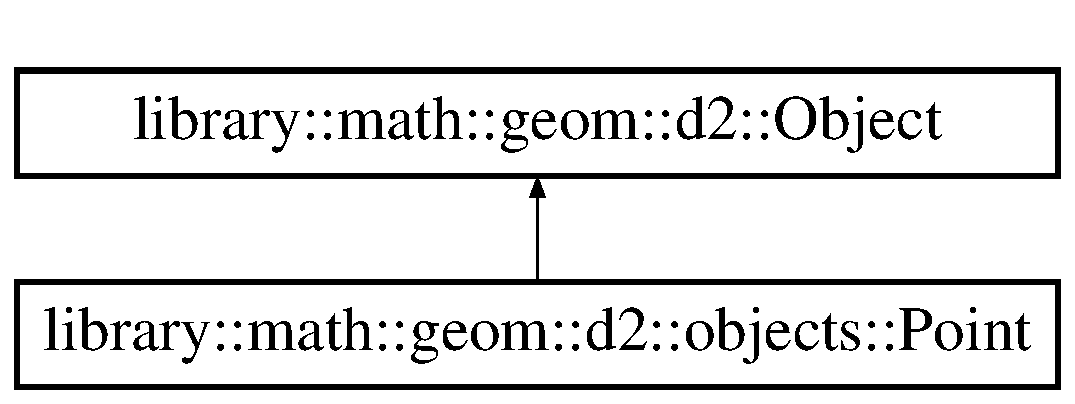
\includegraphics[height=2.000000cm]{classlibrary_1_1math_1_1geom_1_1d2_1_1objects_1_1_point}
\end{center}
\end{figure}
\subsection*{Public Member Functions}
\begin{DoxyCompactItemize}
\item 
\hyperlink{classlibrary_1_1math_1_1geom_1_1d2_1_1objects_1_1_point_a4998aefdf80bdfd967f21d49fa050398}{Point} (const Real \&a\+First\+Coordinate, const Real \&a\+Second\+Coordinate)
\begin{DoxyCompactList}\small\item\em Constructor. \end{DoxyCompactList}\item 
virtual \hyperlink{classlibrary_1_1math_1_1geom_1_1d2_1_1objects_1_1_point}{Point} $\ast$ \hyperlink{classlibrary_1_1math_1_1geom_1_1d2_1_1objects_1_1_point_aa6b55bdbf5a0ce9ec8bc91ca79de3569}{clone} () const override
\begin{DoxyCompactList}\small\item\em Clone point. \end{DoxyCompactList}\item 
bool \hyperlink{classlibrary_1_1math_1_1geom_1_1d2_1_1objects_1_1_point_af5223d8e73deaf75ac248a5d43139628}{operator==} (const \hyperlink{classlibrary_1_1math_1_1geom_1_1d2_1_1objects_1_1_point}{Point} \&a\+Point) const
\begin{DoxyCompactList}\small\item\em Equal to operator. \end{DoxyCompactList}\item 
bool \hyperlink{classlibrary_1_1math_1_1geom_1_1d2_1_1objects_1_1_point_ac3a7bf1647172166e83a016ca32669c3}{operator!=} (const \hyperlink{classlibrary_1_1math_1_1geom_1_1d2_1_1objects_1_1_point}{Point} \&a\+Point) const
\begin{DoxyCompactList}\small\item\em Not equal to operator. \end{DoxyCompactList}\item 
virtual bool \hyperlink{classlibrary_1_1math_1_1geom_1_1d2_1_1objects_1_1_point_ac90251968d8eb11df82e28f6cf095e5c}{is\+Defined} () const override
\begin{DoxyCompactList}\small\item\em Addition operator\+: translate point along vector. \end{DoxyCompactList}\item 
bool \hyperlink{classlibrary_1_1math_1_1geom_1_1d2_1_1objects_1_1_point_aeec1bab241792dc6b6091d9cac36d02e}{is\+Near} (const \hyperlink{classlibrary_1_1math_1_1geom_1_1d2_1_1objects_1_1_point}{Point} \&a\+Point, const Real \&a\+Tolerance) const
\begin{DoxyCompactList}\small\item\em Check if point is near another point. \end{DoxyCompactList}\item 
const Real \& \hyperlink{classlibrary_1_1math_1_1geom_1_1d2_1_1objects_1_1_point_abaaa09e58c97324a44e9d60bcad63171}{x} () const
\begin{DoxyCompactList}\small\item\em Get reference to first coordinate. \end{DoxyCompactList}\item 
const Real \& \hyperlink{classlibrary_1_1math_1_1geom_1_1d2_1_1objects_1_1_point_a088e03daba1ed10a0a3e575ffd1d82fa}{y} () const
\begin{DoxyCompactList}\small\item\em Get reference to second coordinate. \end{DoxyCompactList}\item 
Vector2d \hyperlink{classlibrary_1_1math_1_1geom_1_1d2_1_1objects_1_1_point_a570cc81d15674537baa36e0e1b251612}{as\+Vector} () const
\begin{DoxyCompactList}\small\item\em Get vector representation of point. \end{DoxyCompactList}\item 
Real \hyperlink{classlibrary_1_1math_1_1geom_1_1d2_1_1objects_1_1_point_a1615c904b4f5a1c406cdba97df6445d8}{distance\+To} (const \hyperlink{classlibrary_1_1math_1_1geom_1_1d2_1_1objects_1_1_point}{Point} \&a\+Point) const
\begin{DoxyCompactList}\small\item\em Get distance to another point. \end{DoxyCompactList}\item 
virtual String \hyperlink{classlibrary_1_1math_1_1geom_1_1d2_1_1objects_1_1_point_ae645a37f426dac123d566fb5511d595d}{to\+String} (const \hyperlink{classlibrary_1_1math_1_1geom_1_1d2_1_1_object_ac8cd61dada4960cfee9a469231621b17}{Object\+::\+Format} \&a\+Format=\hyperlink{classlibrary_1_1math_1_1geom_1_1d2_1_1_object_ac8cd61dada4960cfee9a469231621b17aeb6d8ae6f20283755b339c0dc273988b}{Object\+::\+Format\+::\+Standard}, const Integer \&a\+Precision=Integer\+::\+Undefined()) const override
\begin{DoxyCompactList}\small\item\em Get string representation. \end{DoxyCompactList}\item 
virtual void \hyperlink{classlibrary_1_1math_1_1geom_1_1d2_1_1objects_1_1_point_a74bef6325d728e1cb6e70bac0b8d4601}{print} (std\+::ostream \&an\+Output\+Stream, bool display\+Decorators=true) const override
\begin{DoxyCompactList}\small\item\em Print point. \end{DoxyCompactList}\item 
virtual void \hyperlink{classlibrary_1_1math_1_1geom_1_1d2_1_1objects_1_1_point_a71d3ef79dbffcd2568d1a2c6bad807d7}{apply\+Transformation} (const \hyperlink{classlibrary_1_1math_1_1geom_1_1d2_1_1_transformation}{Transformation} \&a\+Transformation) override
\begin{DoxyCompactList}\small\item\em Apply transformation to point. \end{DoxyCompactList}\end{DoxyCompactItemize}
\subsection*{Static Public Member Functions}
\begin{DoxyCompactItemize}
\item 
static \hyperlink{classlibrary_1_1math_1_1geom_1_1d2_1_1objects_1_1_point}{Point} \hyperlink{classlibrary_1_1math_1_1geom_1_1d2_1_1objects_1_1_point_a110a5bba9399abc5408f6c34306040c6}{Undefined} ()
\begin{DoxyCompactList}\small\item\em Constructs an undefined point. \end{DoxyCompactList}\item 
static \hyperlink{classlibrary_1_1math_1_1geom_1_1d2_1_1objects_1_1_point}{Point} \hyperlink{classlibrary_1_1math_1_1geom_1_1d2_1_1objects_1_1_point_ac372ec5b87ab91d58dc515eda2f0fa75}{Origin} ()
\begin{DoxyCompactList}\small\item\em Constructs a point at origin. \end{DoxyCompactList}\item 
static \hyperlink{classlibrary_1_1math_1_1geom_1_1d2_1_1objects_1_1_point}{Point} \hyperlink{classlibrary_1_1math_1_1geom_1_1d2_1_1objects_1_1_point_a3b656a68cb1f75901dc44e109e6eca58}{Vector} (const Vector2d \&a\+Vector)
\begin{DoxyCompactList}\small\item\em Constructs a point from a vector. \end{DoxyCompactList}\end{DoxyCompactItemize}
\subsection*{Additional Inherited Members}


\subsection{Detailed Description}
\hyperlink{classlibrary_1_1math_1_1geom_1_1d2_1_1objects_1_1_point}{Point}. 

https\+://en.wikipedia.\+org/wiki/\+Point\+\_\+(geometry) 

\subsection{Constructor \& Destructor Documentation}
\mbox{\Hypertarget{classlibrary_1_1math_1_1geom_1_1d2_1_1objects_1_1_point_a4998aefdf80bdfd967f21d49fa050398}\label{classlibrary_1_1math_1_1geom_1_1d2_1_1objects_1_1_point_a4998aefdf80bdfd967f21d49fa050398}} 
\index{library\+::math\+::geom\+::d2\+::objects\+::\+Point@{library\+::math\+::geom\+::d2\+::objects\+::\+Point}!Point@{Point}}
\index{Point@{Point}!library\+::math\+::geom\+::d2\+::objects\+::\+Point@{library\+::math\+::geom\+::d2\+::objects\+::\+Point}}
\subsubsection{\texorpdfstring{Point()}{Point()}}
{\footnotesize\ttfamily library\+::math\+::geom\+::d2\+::objects\+::\+Point\+::\+Point (\begin{DoxyParamCaption}\item[{const Real \&}]{a\+First\+Coordinate,  }\item[{const Real \&}]{a\+Second\+Coordinate }\end{DoxyParamCaption})}



Constructor. 


\begin{DoxyCode}
\hyperlink{classlibrary_1_1math_1_1geom_1_1d2_1_1objects_1_1_point_a4998aefdf80bdfd967f21d49fa050398}{Point} point = \{ 0.0, 0.0 \} ;
\end{DoxyCode}



\begin{DoxyParams}[1]{Parameters}
\mbox{\tt in}  & {\em a\+First\+Coordinate} & A first coordinate \\
\hline
\mbox{\tt in}  & {\em a\+Second\+Coordinate} & A second coordinate \\
\hline
\end{DoxyParams}


\subsection{Member Function Documentation}
\mbox{\Hypertarget{classlibrary_1_1math_1_1geom_1_1d2_1_1objects_1_1_point_a71d3ef79dbffcd2568d1a2c6bad807d7}\label{classlibrary_1_1math_1_1geom_1_1d2_1_1objects_1_1_point_a71d3ef79dbffcd2568d1a2c6bad807d7}} 
\index{library\+::math\+::geom\+::d2\+::objects\+::\+Point@{library\+::math\+::geom\+::d2\+::objects\+::\+Point}!apply\+Transformation@{apply\+Transformation}}
\index{apply\+Transformation@{apply\+Transformation}!library\+::math\+::geom\+::d2\+::objects\+::\+Point@{library\+::math\+::geom\+::d2\+::objects\+::\+Point}}
\subsubsection{\texorpdfstring{apply\+Transformation()}{applyTransformation()}}
{\footnotesize\ttfamily void library\+::math\+::geom\+::d2\+::objects\+::\+Point\+::apply\+Transformation (\begin{DoxyParamCaption}\item[{const \hyperlink{classlibrary_1_1math_1_1geom_1_1d2_1_1_transformation}{Transformation} \&}]{a\+Transformation }\end{DoxyParamCaption})\hspace{0.3cm}{\ttfamily [override]}, {\ttfamily [virtual]}}



Apply transformation to point. 


\begin{DoxyParams}[1]{Parameters}
\mbox{\tt in}  & {\em a\+Transformation} & A transformation \\
\hline
\end{DoxyParams}


Implements \hyperlink{classlibrary_1_1math_1_1geom_1_1d2_1_1_object_a289589fb6e9e7a2c4ca4976a1544def5}{library\+::math\+::geom\+::d2\+::\+Object}.

\mbox{\Hypertarget{classlibrary_1_1math_1_1geom_1_1d2_1_1objects_1_1_point_a570cc81d15674537baa36e0e1b251612}\label{classlibrary_1_1math_1_1geom_1_1d2_1_1objects_1_1_point_a570cc81d15674537baa36e0e1b251612}} 
\index{library\+::math\+::geom\+::d2\+::objects\+::\+Point@{library\+::math\+::geom\+::d2\+::objects\+::\+Point}!as\+Vector@{as\+Vector}}
\index{as\+Vector@{as\+Vector}!library\+::math\+::geom\+::d2\+::objects\+::\+Point@{library\+::math\+::geom\+::d2\+::objects\+::\+Point}}
\subsubsection{\texorpdfstring{as\+Vector()}{asVector()}}
{\footnotesize\ttfamily Vector2d library\+::math\+::geom\+::d2\+::objects\+::\+Point\+::as\+Vector (\begin{DoxyParamCaption}{ }\end{DoxyParamCaption}) const}



Get vector representation of point. 

\begin{DoxyReturn}{Returns}
Vector representation of point 
\end{DoxyReturn}
\mbox{\Hypertarget{classlibrary_1_1math_1_1geom_1_1d2_1_1objects_1_1_point_aa6b55bdbf5a0ce9ec8bc91ca79de3569}\label{classlibrary_1_1math_1_1geom_1_1d2_1_1objects_1_1_point_aa6b55bdbf5a0ce9ec8bc91ca79de3569}} 
\index{library\+::math\+::geom\+::d2\+::objects\+::\+Point@{library\+::math\+::geom\+::d2\+::objects\+::\+Point}!clone@{clone}}
\index{clone@{clone}!library\+::math\+::geom\+::d2\+::objects\+::\+Point@{library\+::math\+::geom\+::d2\+::objects\+::\+Point}}
\subsubsection{\texorpdfstring{clone()}{clone()}}
{\footnotesize\ttfamily \hyperlink{classlibrary_1_1math_1_1geom_1_1d2_1_1objects_1_1_point}{Point} $\ast$ library\+::math\+::geom\+::d2\+::objects\+::\+Point\+::clone (\begin{DoxyParamCaption}{ }\end{DoxyParamCaption}) const\hspace{0.3cm}{\ttfamily [override]}, {\ttfamily [virtual]}}



Clone point. 

\begin{DoxyReturn}{Returns}
Pointer to cloned point 
\end{DoxyReturn}


Implements \hyperlink{classlibrary_1_1math_1_1geom_1_1d2_1_1_object_a5c26ae4120edb24f6463d65a9cef247d}{library\+::math\+::geom\+::d2\+::\+Object}.

\mbox{\Hypertarget{classlibrary_1_1math_1_1geom_1_1d2_1_1objects_1_1_point_a1615c904b4f5a1c406cdba97df6445d8}\label{classlibrary_1_1math_1_1geom_1_1d2_1_1objects_1_1_point_a1615c904b4f5a1c406cdba97df6445d8}} 
\index{library\+::math\+::geom\+::d2\+::objects\+::\+Point@{library\+::math\+::geom\+::d2\+::objects\+::\+Point}!distance\+To@{distance\+To}}
\index{distance\+To@{distance\+To}!library\+::math\+::geom\+::d2\+::objects\+::\+Point@{library\+::math\+::geom\+::d2\+::objects\+::\+Point}}
\subsubsection{\texorpdfstring{distance\+To()}{distanceTo()}}
{\footnotesize\ttfamily Real library\+::math\+::geom\+::d2\+::objects\+::\+Point\+::distance\+To (\begin{DoxyParamCaption}\item[{const \hyperlink{classlibrary_1_1math_1_1geom_1_1d2_1_1objects_1_1_point}{Point} \&}]{a\+Point }\end{DoxyParamCaption}) const}



Get distance to another point. 


\begin{DoxyParams}[1]{Parameters}
\mbox{\tt in}  & {\em a\+Point} & A point \\
\hline
\end{DoxyParams}
\begin{DoxyReturn}{Returns}
Distance to point 
\end{DoxyReturn}
\mbox{\Hypertarget{classlibrary_1_1math_1_1geom_1_1d2_1_1objects_1_1_point_ac90251968d8eb11df82e28f6cf095e5c}\label{classlibrary_1_1math_1_1geom_1_1d2_1_1objects_1_1_point_ac90251968d8eb11df82e28f6cf095e5c}} 
\index{library\+::math\+::geom\+::d2\+::objects\+::\+Point@{library\+::math\+::geom\+::d2\+::objects\+::\+Point}!is\+Defined@{is\+Defined}}
\index{is\+Defined@{is\+Defined}!library\+::math\+::geom\+::d2\+::objects\+::\+Point@{library\+::math\+::geom\+::d2\+::objects\+::\+Point}}
\subsubsection{\texorpdfstring{is\+Defined()}{isDefined()}}
{\footnotesize\ttfamily bool library\+::math\+::geom\+::d2\+::objects\+::\+Point\+::is\+Defined (\begin{DoxyParamCaption}{ }\end{DoxyParamCaption}) const\hspace{0.3cm}{\ttfamily [override]}, {\ttfamily [virtual]}}



Addition operator\+: translate point along vector. 


\begin{DoxyCode}
                        \hyperlink{classlibrary_1_1math_1_1geom_1_1d2_1_1objects_1_1_point_a4998aefdf80bdfd967f21d49fa050398}{Point}(0.0, 0.0) + \hyperlink{namespacelibrary_1_1math_1_1obj_a2fa27512c4f4b07db35d602cfdd2c293}{Vector2d}(0.0, 1.0) ; \textcolor{comment}{// [0.0, 1.0]}
    @encode
   
    @param              [in] aVector A translation vector
    @\textcolor{keywordflow}{return}             A point

\hyperlink{classlibrary_1_1math_1_1geom_1_1d2_1_1objects_1_1_point_a4998aefdf80bdfd967f21d49fa050398}{Point}                   operator +                                  (   \textcolor{keyword}{const}   
      \hyperlink{namespacelibrary_1_1math_1_1obj_a2fa27512c4f4b07db35d602cfdd2c293}{Vector2d}&                   aVector                                     ) \textcolor{keyword}{const} ;

    @brief              Subtraction \textcolor{keyword}{operator}: translate point along opposite vector
   
    @code
                        \hyperlink{classlibrary_1_1math_1_1geom_1_1d2_1_1objects_1_1_point_a4998aefdf80bdfd967f21d49fa050398}{Point}(0.0, 1.0) - \hyperlink{namespacelibrary_1_1math_1_1obj_a2fa27512c4f4b07db35d602cfdd2c293}{Vector2d}(0.0, 1.0) ; \textcolor{comment}{// [0.0, 0.0]}
    @encode
   
    @param              [in] aVector A translation vector
    @\textcolor{keywordflow}{return}             A point

\hyperlink{classlibrary_1_1math_1_1geom_1_1d2_1_1objects_1_1_point_a4998aefdf80bdfd967f21d49fa050398}{Point}                   operator -                                  (   \textcolor{keyword}{const}   
      \hyperlink{namespacelibrary_1_1math_1_1obj_a2fa27512c4f4b07db35d602cfdd2c293}{Vector2d}&                   aVector                                     ) \textcolor{keyword}{const} ;

    @brief              Subtraction \textcolor{keyword}{operator}: \textcolor{keyword}{get} translation vector between two points
   
    @code
                        \hyperlink{classlibrary_1_1math_1_1geom_1_1d2_1_1objects_1_1_point_a4998aefdf80bdfd967f21d49fa050398}{Point}(0.0, 1.0) - \hyperlink{classlibrary_1_1math_1_1geom_1_1d2_1_1objects_1_1_point_a4998aefdf80bdfd967f21d49fa050398}{Point}(0.0, 0.0)  ; \textcolor{comment}{// [0.0, 1.0]}
    @encode
   
    @param              [in] aPoint A point
    @\textcolor{keywordflow}{return}             A translation vector

\hyperlink{namespacelibrary_1_1math_1_1obj_a2fa27512c4f4b07db35d602cfdd2c293}{Vector2d}                operator -                                  (   \textcolor{keyword}{const}   
      \hyperlink{classlibrary_1_1math_1_1geom_1_1d2_1_1objects_1_1_point_a4998aefdf80bdfd967f21d49fa050398}{Point}&                      aPoint                                      ) \textcolor{keyword}{const} ;

    @brief              Check \textcolor{keywordflow}{if} point is defined
   
    @code
                        \hyperlink{classlibrary_1_1math_1_1geom_1_1d2_1_1objects_1_1_point_a4998aefdf80bdfd967f21d49fa050398}{Point}(0.0, 0.0).isDefined() ; \textcolor{comment}{// True}
\end{DoxyCode}


\begin{DoxyReturn}{Returns}
True if point is defined 
\end{DoxyReturn}


Implements \hyperlink{classlibrary_1_1math_1_1geom_1_1d2_1_1_object_ae9506254971168a3ca63e1923556b70d}{library\+::math\+::geom\+::d2\+::\+Object}.

\mbox{\Hypertarget{classlibrary_1_1math_1_1geom_1_1d2_1_1objects_1_1_point_aeec1bab241792dc6b6091d9cac36d02e}\label{classlibrary_1_1math_1_1geom_1_1d2_1_1objects_1_1_point_aeec1bab241792dc6b6091d9cac36d02e}} 
\index{library\+::math\+::geom\+::d2\+::objects\+::\+Point@{library\+::math\+::geom\+::d2\+::objects\+::\+Point}!is\+Near@{is\+Near}}
\index{is\+Near@{is\+Near}!library\+::math\+::geom\+::d2\+::objects\+::\+Point@{library\+::math\+::geom\+::d2\+::objects\+::\+Point}}
\subsubsection{\texorpdfstring{is\+Near()}{isNear()}}
{\footnotesize\ttfamily bool library\+::math\+::geom\+::d2\+::objects\+::\+Point\+::is\+Near (\begin{DoxyParamCaption}\item[{const \hyperlink{classlibrary_1_1math_1_1geom_1_1d2_1_1objects_1_1_point}{Point} \&}]{a\+Point,  }\item[{const Real \&}]{a\+Tolerance }\end{DoxyParamCaption}) const}



Check if point is near another point. 


\begin{DoxyCode}
\hyperlink{classlibrary_1_1math_1_1geom_1_1d2_1_1objects_1_1_point_a4998aefdf80bdfd967f21d49fa050398}{Point}(0.0, 0.0).isNear(\hyperlink{classlibrary_1_1math_1_1geom_1_1d2_1_1objects_1_1_point_a4998aefdf80bdfd967f21d49fa050398}{Point}(0.0, 0.0), 1e-15) ; \textcolor{comment}{// True}
\end{DoxyCode}



\begin{DoxyParams}[1]{Parameters}
\mbox{\tt in}  & {\em a\+Point} & A point \\
\hline
\mbox{\tt in}  & {\em a\+Tolerance} & A tolerance \\
\hline
\end{DoxyParams}
\begin{DoxyReturn}{Returns}
True if point is near another point 
\end{DoxyReturn}
\mbox{\Hypertarget{classlibrary_1_1math_1_1geom_1_1d2_1_1objects_1_1_point_ac3a7bf1647172166e83a016ca32669c3}\label{classlibrary_1_1math_1_1geom_1_1d2_1_1objects_1_1_point_ac3a7bf1647172166e83a016ca32669c3}} 
\index{library\+::math\+::geom\+::d2\+::objects\+::\+Point@{library\+::math\+::geom\+::d2\+::objects\+::\+Point}!operator"!=@{operator"!=}}
\index{operator"!=@{operator"!=}!library\+::math\+::geom\+::d2\+::objects\+::\+Point@{library\+::math\+::geom\+::d2\+::objects\+::\+Point}}
\subsubsection{\texorpdfstring{operator"!=()}{operator!=()}}
{\footnotesize\ttfamily bool library\+::math\+::geom\+::d2\+::objects\+::\+Point\+::operator!= (\begin{DoxyParamCaption}\item[{const \hyperlink{classlibrary_1_1math_1_1geom_1_1d2_1_1objects_1_1_point}{Point} \&}]{a\+Point }\end{DoxyParamCaption}) const}



Not equal to operator. 


\begin{DoxyParams}[1]{Parameters}
\mbox{\tt in}  & {\em a\+Point} & A point \\
\hline
\end{DoxyParams}
\begin{DoxyReturn}{Returns}
True if points are not equal 
\end{DoxyReturn}
\mbox{\Hypertarget{classlibrary_1_1math_1_1geom_1_1d2_1_1objects_1_1_point_af5223d8e73deaf75ac248a5d43139628}\label{classlibrary_1_1math_1_1geom_1_1d2_1_1objects_1_1_point_af5223d8e73deaf75ac248a5d43139628}} 
\index{library\+::math\+::geom\+::d2\+::objects\+::\+Point@{library\+::math\+::geom\+::d2\+::objects\+::\+Point}!operator==@{operator==}}
\index{operator==@{operator==}!library\+::math\+::geom\+::d2\+::objects\+::\+Point@{library\+::math\+::geom\+::d2\+::objects\+::\+Point}}
\subsubsection{\texorpdfstring{operator==()}{operator==()}}
{\footnotesize\ttfamily bool library\+::math\+::geom\+::d2\+::objects\+::\+Point\+::operator== (\begin{DoxyParamCaption}\item[{const \hyperlink{classlibrary_1_1math_1_1geom_1_1d2_1_1objects_1_1_point}{Point} \&}]{a\+Point }\end{DoxyParamCaption}) const}



Equal to operator. 


\begin{DoxyParams}[1]{Parameters}
\mbox{\tt in}  & {\em a\+Point} & A point \\
\hline
\end{DoxyParams}
\begin{DoxyReturn}{Returns}
True if points are equal 
\end{DoxyReturn}
\mbox{\Hypertarget{classlibrary_1_1math_1_1geom_1_1d2_1_1objects_1_1_point_ac372ec5b87ab91d58dc515eda2f0fa75}\label{classlibrary_1_1math_1_1geom_1_1d2_1_1objects_1_1_point_ac372ec5b87ab91d58dc515eda2f0fa75}} 
\index{library\+::math\+::geom\+::d2\+::objects\+::\+Point@{library\+::math\+::geom\+::d2\+::objects\+::\+Point}!Origin@{Origin}}
\index{Origin@{Origin}!library\+::math\+::geom\+::d2\+::objects\+::\+Point@{library\+::math\+::geom\+::d2\+::objects\+::\+Point}}
\subsubsection{\texorpdfstring{Origin()}{Origin()}}
{\footnotesize\ttfamily \hyperlink{classlibrary_1_1math_1_1geom_1_1d2_1_1objects_1_1_point}{Point} library\+::math\+::geom\+::d2\+::objects\+::\+Point\+::\+Origin (\begin{DoxyParamCaption}{ }\end{DoxyParamCaption})\hspace{0.3cm}{\ttfamily [static]}}



Constructs a point at origin. 


\begin{DoxyCode}
\hyperlink{classlibrary_1_1math_1_1geom_1_1d2_1_1objects_1_1_point_a4998aefdf80bdfd967f21d49fa050398}{Point} point = \hyperlink{classlibrary_1_1math_1_1geom_1_1d2_1_1objects_1_1_point_ac372ec5b87ab91d58dc515eda2f0fa75}{Point::Origin}() ; \textcolor{comment}{// [0.0, 0.0]}
\end{DoxyCode}


\begin{DoxyReturn}{Returns}
\hyperlink{classlibrary_1_1math_1_1geom_1_1d2_1_1objects_1_1_point}{Point} at origin 
\end{DoxyReturn}
\mbox{\Hypertarget{classlibrary_1_1math_1_1geom_1_1d2_1_1objects_1_1_point_a74bef6325d728e1cb6e70bac0b8d4601}\label{classlibrary_1_1math_1_1geom_1_1d2_1_1objects_1_1_point_a74bef6325d728e1cb6e70bac0b8d4601}} 
\index{library\+::math\+::geom\+::d2\+::objects\+::\+Point@{library\+::math\+::geom\+::d2\+::objects\+::\+Point}!print@{print}}
\index{print@{print}!library\+::math\+::geom\+::d2\+::objects\+::\+Point@{library\+::math\+::geom\+::d2\+::objects\+::\+Point}}
\subsubsection{\texorpdfstring{print()}{print()}}
{\footnotesize\ttfamily void library\+::math\+::geom\+::d2\+::objects\+::\+Point\+::print (\begin{DoxyParamCaption}\item[{std\+::ostream \&}]{an\+Output\+Stream,  }\item[{bool}]{display\+Decorators = {\ttfamily true} }\end{DoxyParamCaption}) const\hspace{0.3cm}{\ttfamily [override]}, {\ttfamily [virtual]}}



Print point. 


\begin{DoxyParams}[1]{Parameters}
\mbox{\tt in}  & {\em an\+Output\+Stream} & An output stream \\
\hline
\mbox{\tt in}  & {\em (optional)} & display\+Decorators If true, display decorators \\
\hline
\end{DoxyParams}


Implements \hyperlink{classlibrary_1_1math_1_1geom_1_1d2_1_1_object_a834bbf59cf1c483d1dc7b0966b1e1ab3}{library\+::math\+::geom\+::d2\+::\+Object}.

\mbox{\Hypertarget{classlibrary_1_1math_1_1geom_1_1d2_1_1objects_1_1_point_ae645a37f426dac123d566fb5511d595d}\label{classlibrary_1_1math_1_1geom_1_1d2_1_1objects_1_1_point_ae645a37f426dac123d566fb5511d595d}} 
\index{library\+::math\+::geom\+::d2\+::objects\+::\+Point@{library\+::math\+::geom\+::d2\+::objects\+::\+Point}!to\+String@{to\+String}}
\index{to\+String@{to\+String}!library\+::math\+::geom\+::d2\+::objects\+::\+Point@{library\+::math\+::geom\+::d2\+::objects\+::\+Point}}
\subsubsection{\texorpdfstring{to\+String()}{toString()}}
{\footnotesize\ttfamily String library\+::math\+::geom\+::d2\+::objects\+::\+Point\+::to\+String (\begin{DoxyParamCaption}\item[{const \hyperlink{classlibrary_1_1math_1_1geom_1_1d2_1_1_object_ac8cd61dada4960cfee9a469231621b17}{Object\+::\+Format} \&}]{a\+Format = {\ttfamily \hyperlink{classlibrary_1_1math_1_1geom_1_1d2_1_1_object_ac8cd61dada4960cfee9a469231621b17aeb6d8ae6f20283755b339c0dc273988b}{Object\+::\+Format\+::\+Standard}},  }\item[{const Integer \&}]{a\+Precision = {\ttfamily Integer\+:\+:Undefined()} }\end{DoxyParamCaption}) const\hspace{0.3cm}{\ttfamily [override]}, {\ttfamily [virtual]}}



Get string representation. 


\begin{DoxyParams}[1]{Parameters}
\mbox{\tt in}  & {\em a\+Format} & A format \\
\hline
\mbox{\tt in}  & {\em (optional)} & a\+Precision A precision \\
\hline
\end{DoxyParams}
\begin{DoxyReturn}{Returns}
String representation 
\end{DoxyReturn}


Implements \hyperlink{classlibrary_1_1math_1_1geom_1_1d2_1_1_object_acdd76b3637732a249536b609dbe3f0eb}{library\+::math\+::geom\+::d2\+::\+Object}.

\mbox{\Hypertarget{classlibrary_1_1math_1_1geom_1_1d2_1_1objects_1_1_point_a110a5bba9399abc5408f6c34306040c6}\label{classlibrary_1_1math_1_1geom_1_1d2_1_1objects_1_1_point_a110a5bba9399abc5408f6c34306040c6}} 
\index{library\+::math\+::geom\+::d2\+::objects\+::\+Point@{library\+::math\+::geom\+::d2\+::objects\+::\+Point}!Undefined@{Undefined}}
\index{Undefined@{Undefined}!library\+::math\+::geom\+::d2\+::objects\+::\+Point@{library\+::math\+::geom\+::d2\+::objects\+::\+Point}}
\subsubsection{\texorpdfstring{Undefined()}{Undefined()}}
{\footnotesize\ttfamily \hyperlink{classlibrary_1_1math_1_1geom_1_1d2_1_1objects_1_1_point}{Point} library\+::math\+::geom\+::d2\+::objects\+::\+Point\+::\+Undefined (\begin{DoxyParamCaption}{ }\end{DoxyParamCaption})\hspace{0.3cm}{\ttfamily [static]}}



Constructs an undefined point. 


\begin{DoxyCode}
\hyperlink{classlibrary_1_1math_1_1geom_1_1d2_1_1objects_1_1_point_a4998aefdf80bdfd967f21d49fa050398}{Point} point = \hyperlink{classlibrary_1_1math_1_1geom_1_1d2_1_1objects_1_1_point_a110a5bba9399abc5408f6c34306040c6}{Point::Undefined}() ; \textcolor{comment}{// Undefined}
\end{DoxyCode}


\begin{DoxyReturn}{Returns}
Undefined point 
\end{DoxyReturn}
\mbox{\Hypertarget{classlibrary_1_1math_1_1geom_1_1d2_1_1objects_1_1_point_a3b656a68cb1f75901dc44e109e6eca58}\label{classlibrary_1_1math_1_1geom_1_1d2_1_1objects_1_1_point_a3b656a68cb1f75901dc44e109e6eca58}} 
\index{library\+::math\+::geom\+::d2\+::objects\+::\+Point@{library\+::math\+::geom\+::d2\+::objects\+::\+Point}!Vector@{Vector}}
\index{Vector@{Vector}!library\+::math\+::geom\+::d2\+::objects\+::\+Point@{library\+::math\+::geom\+::d2\+::objects\+::\+Point}}
\subsubsection{\texorpdfstring{Vector()}{Vector()}}
{\footnotesize\ttfamily \hyperlink{classlibrary_1_1math_1_1geom_1_1d2_1_1objects_1_1_point}{Point} library\+::math\+::geom\+::d2\+::objects\+::\+Point\+::\+Vector (\begin{DoxyParamCaption}\item[{const Vector2d \&}]{a\+Vector }\end{DoxyParamCaption})\hspace{0.3cm}{\ttfamily [static]}}



Constructs a point from a vector. 


\begin{DoxyCode}
\hyperlink{classlibrary_1_1math_1_1geom_1_1d2_1_1objects_1_1_point_a4998aefdf80bdfd967f21d49fa050398}{Point} point = \hyperlink{classlibrary_1_1math_1_1geom_1_1d2_1_1objects_1_1_point_a3b656a68cb1f75901dc44e109e6eca58}{Point::Vector}(\{ 0.0, 0.0 \}) ; \textcolor{comment}{// [0.0, 0.0]}
\end{DoxyCode}


\begin{DoxyReturn}{Returns}
\hyperlink{classlibrary_1_1math_1_1geom_1_1d2_1_1objects_1_1_point}{Point} 
\end{DoxyReturn}
\mbox{\Hypertarget{classlibrary_1_1math_1_1geom_1_1d2_1_1objects_1_1_point_abaaa09e58c97324a44e9d60bcad63171}\label{classlibrary_1_1math_1_1geom_1_1d2_1_1objects_1_1_point_abaaa09e58c97324a44e9d60bcad63171}} 
\index{library\+::math\+::geom\+::d2\+::objects\+::\+Point@{library\+::math\+::geom\+::d2\+::objects\+::\+Point}!x@{x}}
\index{x@{x}!library\+::math\+::geom\+::d2\+::objects\+::\+Point@{library\+::math\+::geom\+::d2\+::objects\+::\+Point}}
\subsubsection{\texorpdfstring{x()}{x()}}
{\footnotesize\ttfamily const Real \& library\+::math\+::geom\+::d2\+::objects\+::\+Point\+::x (\begin{DoxyParamCaption}{ }\end{DoxyParamCaption}) const}



Get reference to first coordinate. 


\begin{DoxyCode}
\hyperlink{classlibrary_1_1math_1_1geom_1_1d2_1_1objects_1_1_point_a4998aefdf80bdfd967f21d49fa050398}{Point}(1.0, 2.0).x() ; \textcolor{comment}{// &1.0}
\end{DoxyCode}


\begin{DoxyReturn}{Returns}
Reference to first coordinate 
\end{DoxyReturn}
\mbox{\Hypertarget{classlibrary_1_1math_1_1geom_1_1d2_1_1objects_1_1_point_a088e03daba1ed10a0a3e575ffd1d82fa}\label{classlibrary_1_1math_1_1geom_1_1d2_1_1objects_1_1_point_a088e03daba1ed10a0a3e575ffd1d82fa}} 
\index{library\+::math\+::geom\+::d2\+::objects\+::\+Point@{library\+::math\+::geom\+::d2\+::objects\+::\+Point}!y@{y}}
\index{y@{y}!library\+::math\+::geom\+::d2\+::objects\+::\+Point@{library\+::math\+::geom\+::d2\+::objects\+::\+Point}}
\subsubsection{\texorpdfstring{y()}{y()}}
{\footnotesize\ttfamily const Real \& library\+::math\+::geom\+::d2\+::objects\+::\+Point\+::y (\begin{DoxyParamCaption}{ }\end{DoxyParamCaption}) const}



Get reference to second coordinate. 


\begin{DoxyCode}
\hyperlink{classlibrary_1_1math_1_1geom_1_1d2_1_1objects_1_1_point_a4998aefdf80bdfd967f21d49fa050398}{Point}(1.0, 2.0).y() ; \textcolor{comment}{// &2.0}
\end{DoxyCode}


\begin{DoxyReturn}{Returns}
Reference to second coordinate 
\end{DoxyReturn}


The documentation for this class was generated from the following files\+:\begin{DoxyCompactItemize}
\item 
include/\+Library/\+Mathematics/\+Geometry/2\+D/\+Objects/\hyperlink{2_d_2_objects_2_point_8hpp}{Point.\+hpp}\item 
src/\+Library/\+Mathematics/\+Geometry/2\+D/\+Objects/\hyperlink{2_d_2_objects_2_point_8cpp}{Point.\+cpp}\end{DoxyCompactItemize}

\hypertarget{classlibrary_1_1math_1_1geom_1_1d3_1_1objects_1_1_point_set}{}\section{library\+:\+:math\+:\+:geom\+:\+:d3\+:\+:objects\+:\+:Point\+Set Class Reference}
\label{classlibrary_1_1math_1_1geom_1_1d3_1_1objects_1_1_point_set}\index{library\+::math\+::geom\+::d3\+::objects\+::\+Point\+Set@{library\+::math\+::geom\+::d3\+::objects\+::\+Point\+Set}}


\hyperlink{classlibrary_1_1math_1_1geom_1_1d3_1_1objects_1_1_point}{Point} set.  




{\ttfamily \#include $<$Point\+Set.\+hpp$>$}

Inheritance diagram for library\+:\+:math\+:\+:geom\+:\+:d3\+:\+:objects\+:\+:Point\+Set\+:\begin{figure}[H]
\begin{center}
\leavevmode
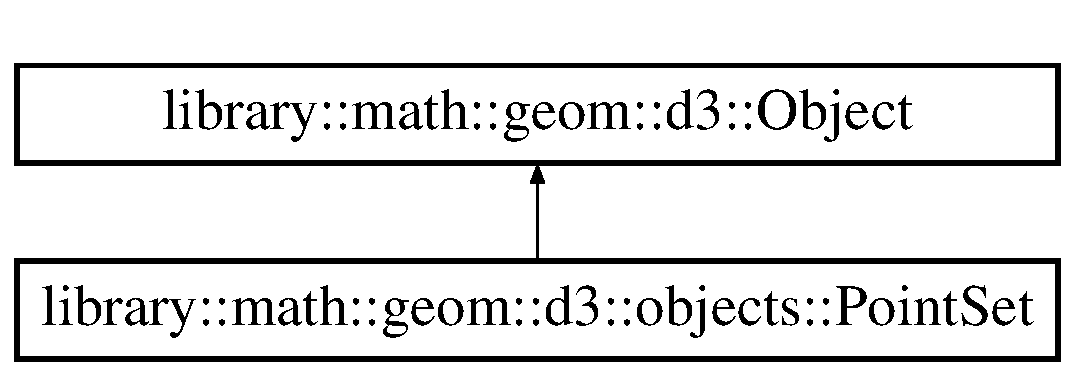
\includegraphics[height=2.000000cm]{classlibrary_1_1math_1_1geom_1_1d3_1_1objects_1_1_point_set}
\end{center}
\end{figure}
\subsection*{Classes}
\begin{DoxyCompactItemize}
\item 
struct \hyperlink{structlibrary_1_1math_1_1geom_1_1d3_1_1objects_1_1_point_set_1_1_hasher}{Hasher}
\begin{DoxyCompactList}\small\item\em \hyperlink{classlibrary_1_1math_1_1geom_1_1d3_1_1objects_1_1_point}{Point} hasher. \end{DoxyCompactList}\end{DoxyCompactItemize}
\subsection*{Public Types}
\begin{DoxyCompactItemize}
\item 
typedef std\+::unordered\+\_\+set$<$ \hyperlink{classlibrary_1_1math_1_1geom_1_1d3_1_1objects_1_1_point}{Point}, \hyperlink{structlibrary_1_1math_1_1geom_1_1d3_1_1objects_1_1_point_set_1_1_hasher}{Point\+Set\+::\+Hasher} $>$ \hyperlink{classlibrary_1_1math_1_1geom_1_1d3_1_1objects_1_1_point_set_ac1aed08551a4cc9556b4b49f88ae35d4}{Container}
\item 
typedef Point\+Set\+::\+Container\+::const\+\_\+iterator \hyperlink{classlibrary_1_1math_1_1geom_1_1d3_1_1objects_1_1_point_set_a7b7fade95484b653ec27ad082ffc8064}{Const\+Iterator}
\end{DoxyCompactItemize}
\subsection*{Public Member Functions}
\begin{DoxyCompactItemize}
\item 
\hyperlink{classlibrary_1_1math_1_1geom_1_1d3_1_1objects_1_1_point_set_a6f9624b8c6bb3aa9d57a35a6fa2e0fba}{Point\+Set} (const Array$<$ \hyperlink{classlibrary_1_1math_1_1geom_1_1d3_1_1objects_1_1_point}{Point} $>$ \&a\+Point\+Array)
\begin{DoxyCompactList}\small\item\em Constructor. \end{DoxyCompactList}\item 
virtual \hyperlink{classlibrary_1_1math_1_1geom_1_1d3_1_1objects_1_1_point_set}{Point\+Set} $\ast$ \hyperlink{classlibrary_1_1math_1_1geom_1_1d3_1_1objects_1_1_point_set_ab7c4ec1d48795973be648f0907b84484}{clone} () const override
\begin{DoxyCompactList}\small\item\em Clone point set. \end{DoxyCompactList}\item 
bool \hyperlink{classlibrary_1_1math_1_1geom_1_1d3_1_1objects_1_1_point_set_afd9dc122c96bb0807bbe5ba6d84be519}{operator==} (const \hyperlink{classlibrary_1_1math_1_1geom_1_1d3_1_1objects_1_1_point_set}{Point\+Set} \&a\+Point\+Set) const
\begin{DoxyCompactList}\small\item\em Equal to operator. \end{DoxyCompactList}\item 
bool \hyperlink{classlibrary_1_1math_1_1geom_1_1d3_1_1objects_1_1_point_set_aeec01caca12c9c4eaec2c7b8694bfb10}{operator!=} (const \hyperlink{classlibrary_1_1math_1_1geom_1_1d3_1_1objects_1_1_point_set}{Point\+Set} \&a\+Point\+Set) const
\begin{DoxyCompactList}\small\item\em Not equal to operator. \end{DoxyCompactList}\item 
virtual bool \hyperlink{classlibrary_1_1math_1_1geom_1_1d3_1_1objects_1_1_point_set_abeb7f866a32d25448d1ddb00c6c5e7b0}{is\+Defined} () const override
\begin{DoxyCompactList}\small\item\em Check if point set is defined. \end{DoxyCompactList}\item 
bool \hyperlink{classlibrary_1_1math_1_1geom_1_1d3_1_1objects_1_1_point_set_a1bffbfee716ad81a0a475fa2f7d69f9b}{is\+Empty} () const
\begin{DoxyCompactList}\small\item\em Check if point set is empty. \end{DoxyCompactList}\item 
bool \hyperlink{classlibrary_1_1math_1_1geom_1_1d3_1_1objects_1_1_point_set_acffd730ba7d03b3d1e662fa9cdc61813}{is\+Near} (const \hyperlink{classlibrary_1_1math_1_1geom_1_1d3_1_1objects_1_1_point_set}{Point\+Set} \&a\+Point\+Set, const Real \&a\+Tolerance) const
\begin{DoxyCompactList}\small\item\em Check if point set is near another point set. \end{DoxyCompactList}\item 
Size \hyperlink{classlibrary_1_1math_1_1geom_1_1d3_1_1objects_1_1_point_set_ae112a693107884e5d227bfb99f684fea}{get\+Size} () const
\begin{DoxyCompactList}\small\item\em Get size of point set. \end{DoxyCompactList}\item 
\hyperlink{classlibrary_1_1math_1_1geom_1_1d3_1_1objects_1_1_point}{Point} \hyperlink{classlibrary_1_1math_1_1geom_1_1d3_1_1objects_1_1_point_set_a0f2fa4053eec2d5c82cc5b72fb59f1e1}{get\+Point\+Closest\+To} (const \hyperlink{classlibrary_1_1math_1_1geom_1_1d3_1_1objects_1_1_point}{Point} \&a\+Point) const
\begin{DoxyCompactList}\small\item\em Get point closest to another point. \end{DoxyCompactList}\item 
virtual void \hyperlink{classlibrary_1_1math_1_1geom_1_1d3_1_1objects_1_1_point_set_ab1a24422b85249c21feb603025140c1a}{print} (std\+::ostream \&an\+Output\+Stream, bool display\+Decorators=true) const override
\begin{DoxyCompactList}\small\item\em Print point. \end{DoxyCompactList}\item 
\hyperlink{classlibrary_1_1math_1_1geom_1_1d3_1_1objects_1_1_point_set_a7b7fade95484b653ec27ad082ffc8064}{Point\+Set\+::\+Const\+Iterator} \hyperlink{classlibrary_1_1math_1_1geom_1_1d3_1_1objects_1_1_point_set_af81fd640cf4b1804c7c456ce4dbcf2ab}{begin} () const
\begin{DoxyCompactList}\small\item\em Get begin const iterator. \end{DoxyCompactList}\item 
\hyperlink{classlibrary_1_1math_1_1geom_1_1d3_1_1objects_1_1_point_set_a7b7fade95484b653ec27ad082ffc8064}{Point\+Set\+::\+Const\+Iterator} \hyperlink{classlibrary_1_1math_1_1geom_1_1d3_1_1objects_1_1_point_set_ae9f66fcbe937005a418238929048f587}{end} () const
\begin{DoxyCompactList}\small\item\em Get end const iterator. \end{DoxyCompactList}\item 
virtual void \hyperlink{classlibrary_1_1math_1_1geom_1_1d3_1_1objects_1_1_point_set_aa747a6169cd9c14011c8249a728c3c48}{apply\+Transformation} (const \hyperlink{classlibrary_1_1math_1_1geom_1_1d3_1_1_transformation}{Transformation} \&a\+Transformation) override
\begin{DoxyCompactList}\small\item\em Apply transformation to point set. \end{DoxyCompactList}\end{DoxyCompactItemize}
\subsection*{Static Public Member Functions}
\begin{DoxyCompactItemize}
\item 
static \hyperlink{classlibrary_1_1math_1_1geom_1_1d3_1_1objects_1_1_point_set}{Point\+Set} \hyperlink{classlibrary_1_1math_1_1geom_1_1d3_1_1objects_1_1_point_set_af4b649e6c97106bf9f54b2213f10484a}{Empty} ()
\begin{DoxyCompactList}\small\item\em Constructs an empty point set. \end{DoxyCompactList}\end{DoxyCompactItemize}


\subsection{Detailed Description}
\hyperlink{classlibrary_1_1math_1_1geom_1_1d3_1_1objects_1_1_point}{Point} set. 

\subsection{Member Typedef Documentation}
\mbox{\Hypertarget{classlibrary_1_1math_1_1geom_1_1d3_1_1objects_1_1_point_set_a7b7fade95484b653ec27ad082ffc8064}\label{classlibrary_1_1math_1_1geom_1_1d3_1_1objects_1_1_point_set_a7b7fade95484b653ec27ad082ffc8064}} 
\index{library\+::math\+::geom\+::d3\+::objects\+::\+Point\+Set@{library\+::math\+::geom\+::d3\+::objects\+::\+Point\+Set}!Const\+Iterator@{Const\+Iterator}}
\index{Const\+Iterator@{Const\+Iterator}!library\+::math\+::geom\+::d3\+::objects\+::\+Point\+Set@{library\+::math\+::geom\+::d3\+::objects\+::\+Point\+Set}}
\subsubsection{\texorpdfstring{Const\+Iterator}{ConstIterator}}
{\footnotesize\ttfamily typedef Point\+Set\+::\+Container\+::const\+\_\+iterator \hyperlink{classlibrary_1_1math_1_1geom_1_1d3_1_1objects_1_1_point_set_a7b7fade95484b653ec27ad082ffc8064}{library\+::math\+::geom\+::d3\+::objects\+::\+Point\+Set\+::\+Const\+Iterator}}

\mbox{\Hypertarget{classlibrary_1_1math_1_1geom_1_1d3_1_1objects_1_1_point_set_ac1aed08551a4cc9556b4b49f88ae35d4}\label{classlibrary_1_1math_1_1geom_1_1d3_1_1objects_1_1_point_set_ac1aed08551a4cc9556b4b49f88ae35d4}} 
\index{library\+::math\+::geom\+::d3\+::objects\+::\+Point\+Set@{library\+::math\+::geom\+::d3\+::objects\+::\+Point\+Set}!Container@{Container}}
\index{Container@{Container}!library\+::math\+::geom\+::d3\+::objects\+::\+Point\+Set@{library\+::math\+::geom\+::d3\+::objects\+::\+Point\+Set}}
\subsubsection{\texorpdfstring{Container}{Container}}
{\footnotesize\ttfamily typedef std\+::unordered\+\_\+set$<$\hyperlink{classlibrary_1_1math_1_1geom_1_1d3_1_1objects_1_1_point}{Point}, \hyperlink{structlibrary_1_1math_1_1geom_1_1d3_1_1objects_1_1_point_set_1_1_hasher}{Point\+Set\+::\+Hasher}$>$ \hyperlink{classlibrary_1_1math_1_1geom_1_1d3_1_1objects_1_1_point_set_ac1aed08551a4cc9556b4b49f88ae35d4}{library\+::math\+::geom\+::d3\+::objects\+::\+Point\+Set\+::\+Container}}



\subsection{Constructor \& Destructor Documentation}
\mbox{\Hypertarget{classlibrary_1_1math_1_1geom_1_1d3_1_1objects_1_1_point_set_a6f9624b8c6bb3aa9d57a35a6fa2e0fba}\label{classlibrary_1_1math_1_1geom_1_1d3_1_1objects_1_1_point_set_a6f9624b8c6bb3aa9d57a35a6fa2e0fba}} 
\index{library\+::math\+::geom\+::d3\+::objects\+::\+Point\+Set@{library\+::math\+::geom\+::d3\+::objects\+::\+Point\+Set}!Point\+Set@{Point\+Set}}
\index{Point\+Set@{Point\+Set}!library\+::math\+::geom\+::d3\+::objects\+::\+Point\+Set@{library\+::math\+::geom\+::d3\+::objects\+::\+Point\+Set}}
\subsubsection{\texorpdfstring{Point\+Set()}{PointSet()}}
{\footnotesize\ttfamily library\+::math\+::geom\+::d3\+::objects\+::\+Point\+Set\+::\+Point\+Set (\begin{DoxyParamCaption}\item[{const Array$<$ \hyperlink{classlibrary_1_1math_1_1geom_1_1d3_1_1objects_1_1_point}{Point} $>$ \&}]{a\+Point\+Array }\end{DoxyParamCaption})}



Constructor. 


\begin{DoxyCode}
\hyperlink{classlibrary_1_1math_1_1geom_1_1d3_1_1objects_1_1_point_set_a6f9624b8c6bb3aa9d57a35a6fa2e0fba}{PointSet} pointSet(\{ \{ 0.0, 0.0, 0.0 \}, \{ 0.0, 0.0, 1.0 \} \}) ;
\end{DoxyCode}



\begin{DoxyParams}[1]{Parameters}
\mbox{\tt in}  & {\em a\+Point\+Array} & A point array \\
\hline
\end{DoxyParams}


\subsection{Member Function Documentation}
\mbox{\Hypertarget{classlibrary_1_1math_1_1geom_1_1d3_1_1objects_1_1_point_set_aa747a6169cd9c14011c8249a728c3c48}\label{classlibrary_1_1math_1_1geom_1_1d3_1_1objects_1_1_point_set_aa747a6169cd9c14011c8249a728c3c48}} 
\index{library\+::math\+::geom\+::d3\+::objects\+::\+Point\+Set@{library\+::math\+::geom\+::d3\+::objects\+::\+Point\+Set}!apply\+Transformation@{apply\+Transformation}}
\index{apply\+Transformation@{apply\+Transformation}!library\+::math\+::geom\+::d3\+::objects\+::\+Point\+Set@{library\+::math\+::geom\+::d3\+::objects\+::\+Point\+Set}}
\subsubsection{\texorpdfstring{apply\+Transformation()}{applyTransformation()}}
{\footnotesize\ttfamily void library\+::math\+::geom\+::d3\+::objects\+::\+Point\+Set\+::apply\+Transformation (\begin{DoxyParamCaption}\item[{const \hyperlink{classlibrary_1_1math_1_1geom_1_1d3_1_1_transformation}{Transformation} \&}]{a\+Transformation }\end{DoxyParamCaption})\hspace{0.3cm}{\ttfamily [override]}, {\ttfamily [virtual]}}



Apply transformation to point set. 


\begin{DoxyParams}[1]{Parameters}
\mbox{\tt in}  & {\em a\+Transformation} & A transformation \\
\hline
\end{DoxyParams}


Implements \hyperlink{classlibrary_1_1math_1_1geom_1_1d3_1_1_object_a5fc47b1ee5d9a28efc6010d3d1512470}{library\+::math\+::geom\+::d3\+::\+Object}.

\mbox{\Hypertarget{classlibrary_1_1math_1_1geom_1_1d3_1_1objects_1_1_point_set_af81fd640cf4b1804c7c456ce4dbcf2ab}\label{classlibrary_1_1math_1_1geom_1_1d3_1_1objects_1_1_point_set_af81fd640cf4b1804c7c456ce4dbcf2ab}} 
\index{library\+::math\+::geom\+::d3\+::objects\+::\+Point\+Set@{library\+::math\+::geom\+::d3\+::objects\+::\+Point\+Set}!begin@{begin}}
\index{begin@{begin}!library\+::math\+::geom\+::d3\+::objects\+::\+Point\+Set@{library\+::math\+::geom\+::d3\+::objects\+::\+Point\+Set}}
\subsubsection{\texorpdfstring{begin()}{begin()}}
{\footnotesize\ttfamily \hyperlink{classlibrary_1_1math_1_1geom_1_1d3_1_1objects_1_1_point_set_a7b7fade95484b653ec27ad082ffc8064}{Point\+Set\+::\+Const\+Iterator} library\+::math\+::geom\+::d3\+::objects\+::\+Point\+Set\+::begin (\begin{DoxyParamCaption}{ }\end{DoxyParamCaption}) const}



Get begin const iterator. 

\begin{DoxyReturn}{Returns}
Begin const iterator 
\end{DoxyReturn}
\mbox{\Hypertarget{classlibrary_1_1math_1_1geom_1_1d3_1_1objects_1_1_point_set_ab7c4ec1d48795973be648f0907b84484}\label{classlibrary_1_1math_1_1geom_1_1d3_1_1objects_1_1_point_set_ab7c4ec1d48795973be648f0907b84484}} 
\index{library\+::math\+::geom\+::d3\+::objects\+::\+Point\+Set@{library\+::math\+::geom\+::d3\+::objects\+::\+Point\+Set}!clone@{clone}}
\index{clone@{clone}!library\+::math\+::geom\+::d3\+::objects\+::\+Point\+Set@{library\+::math\+::geom\+::d3\+::objects\+::\+Point\+Set}}
\subsubsection{\texorpdfstring{clone()}{clone()}}
{\footnotesize\ttfamily \hyperlink{classlibrary_1_1math_1_1geom_1_1d3_1_1objects_1_1_point_set}{Point\+Set} $\ast$ library\+::math\+::geom\+::d3\+::objects\+::\+Point\+Set\+::clone (\begin{DoxyParamCaption}{ }\end{DoxyParamCaption}) const\hspace{0.3cm}{\ttfamily [override]}, {\ttfamily [virtual]}}



Clone point set. 

\begin{DoxyReturn}{Returns}
Pointer to cloned point set 
\end{DoxyReturn}


Implements \hyperlink{classlibrary_1_1math_1_1geom_1_1d3_1_1_object_a1a784c6b359e0eb97cd34fabc42f2f3f}{library\+::math\+::geom\+::d3\+::\+Object}.

\mbox{\Hypertarget{classlibrary_1_1math_1_1geom_1_1d3_1_1objects_1_1_point_set_af4b649e6c97106bf9f54b2213f10484a}\label{classlibrary_1_1math_1_1geom_1_1d3_1_1objects_1_1_point_set_af4b649e6c97106bf9f54b2213f10484a}} 
\index{library\+::math\+::geom\+::d3\+::objects\+::\+Point\+Set@{library\+::math\+::geom\+::d3\+::objects\+::\+Point\+Set}!Empty@{Empty}}
\index{Empty@{Empty}!library\+::math\+::geom\+::d3\+::objects\+::\+Point\+Set@{library\+::math\+::geom\+::d3\+::objects\+::\+Point\+Set}}
\subsubsection{\texorpdfstring{Empty()}{Empty()}}
{\footnotesize\ttfamily \hyperlink{classlibrary_1_1math_1_1geom_1_1d3_1_1objects_1_1_point_set}{Point\+Set} library\+::math\+::geom\+::d3\+::objects\+::\+Point\+Set\+::\+Empty (\begin{DoxyParamCaption}{ }\end{DoxyParamCaption})\hspace{0.3cm}{\ttfamily [static]}}



Constructs an empty point set. 


\begin{DoxyCode}
\hyperlink{classlibrary_1_1math_1_1geom_1_1d3_1_1objects_1_1_point_set_a6f9624b8c6bb3aa9d57a35a6fa2e0fba}{PointSet} pointSet = \hyperlink{classlibrary_1_1math_1_1geom_1_1d3_1_1objects_1_1_point_set_af4b649e6c97106bf9f54b2213f10484a}{PointSet::Empty}() ;
\end{DoxyCode}


\begin{DoxyReturn}{Returns}
Empty point set 
\end{DoxyReturn}
\mbox{\Hypertarget{classlibrary_1_1math_1_1geom_1_1d3_1_1objects_1_1_point_set_ae9f66fcbe937005a418238929048f587}\label{classlibrary_1_1math_1_1geom_1_1d3_1_1objects_1_1_point_set_ae9f66fcbe937005a418238929048f587}} 
\index{library\+::math\+::geom\+::d3\+::objects\+::\+Point\+Set@{library\+::math\+::geom\+::d3\+::objects\+::\+Point\+Set}!end@{end}}
\index{end@{end}!library\+::math\+::geom\+::d3\+::objects\+::\+Point\+Set@{library\+::math\+::geom\+::d3\+::objects\+::\+Point\+Set}}
\subsubsection{\texorpdfstring{end()}{end()}}
{\footnotesize\ttfamily \hyperlink{classlibrary_1_1math_1_1geom_1_1d3_1_1objects_1_1_point_set_a7b7fade95484b653ec27ad082ffc8064}{Point\+Set\+::\+Const\+Iterator} library\+::math\+::geom\+::d3\+::objects\+::\+Point\+Set\+::end (\begin{DoxyParamCaption}{ }\end{DoxyParamCaption}) const}



Get end const iterator. 

\begin{DoxyReturn}{Returns}
End const iterator 
\end{DoxyReturn}
\mbox{\Hypertarget{classlibrary_1_1math_1_1geom_1_1d3_1_1objects_1_1_point_set_a0f2fa4053eec2d5c82cc5b72fb59f1e1}\label{classlibrary_1_1math_1_1geom_1_1d3_1_1objects_1_1_point_set_a0f2fa4053eec2d5c82cc5b72fb59f1e1}} 
\index{library\+::math\+::geom\+::d3\+::objects\+::\+Point\+Set@{library\+::math\+::geom\+::d3\+::objects\+::\+Point\+Set}!get\+Point\+Closest\+To@{get\+Point\+Closest\+To}}
\index{get\+Point\+Closest\+To@{get\+Point\+Closest\+To}!library\+::math\+::geom\+::d3\+::objects\+::\+Point\+Set@{library\+::math\+::geom\+::d3\+::objects\+::\+Point\+Set}}
\subsubsection{\texorpdfstring{get\+Point\+Closest\+To()}{getPointClosestTo()}}
{\footnotesize\ttfamily \hyperlink{classlibrary_1_1math_1_1geom_1_1d3_1_1objects_1_1_point}{Point} library\+::math\+::geom\+::d3\+::objects\+::\+Point\+Set\+::get\+Point\+Closest\+To (\begin{DoxyParamCaption}\item[{const \hyperlink{classlibrary_1_1math_1_1geom_1_1d3_1_1objects_1_1_point}{Point} \&}]{a\+Point }\end{DoxyParamCaption}) const}



Get point closest to another point. 


\begin{DoxyParams}[1]{Parameters}
\mbox{\tt in}  & {\em a\+Point} & A point \\
\hline
\end{DoxyParams}
\begin{DoxyReturn}{Returns}
Closest point 
\end{DoxyReturn}
\mbox{\Hypertarget{classlibrary_1_1math_1_1geom_1_1d3_1_1objects_1_1_point_set_ae112a693107884e5d227bfb99f684fea}\label{classlibrary_1_1math_1_1geom_1_1d3_1_1objects_1_1_point_set_ae112a693107884e5d227bfb99f684fea}} 
\index{library\+::math\+::geom\+::d3\+::objects\+::\+Point\+Set@{library\+::math\+::geom\+::d3\+::objects\+::\+Point\+Set}!get\+Size@{get\+Size}}
\index{get\+Size@{get\+Size}!library\+::math\+::geom\+::d3\+::objects\+::\+Point\+Set@{library\+::math\+::geom\+::d3\+::objects\+::\+Point\+Set}}
\subsubsection{\texorpdfstring{get\+Size()}{getSize()}}
{\footnotesize\ttfamily Size library\+::math\+::geom\+::d3\+::objects\+::\+Point\+Set\+::get\+Size (\begin{DoxyParamCaption}{ }\end{DoxyParamCaption}) const}



Get size of point set. 

\begin{DoxyReturn}{Returns}
Size of point set 
\end{DoxyReturn}
\mbox{\Hypertarget{classlibrary_1_1math_1_1geom_1_1d3_1_1objects_1_1_point_set_abeb7f866a32d25448d1ddb00c6c5e7b0}\label{classlibrary_1_1math_1_1geom_1_1d3_1_1objects_1_1_point_set_abeb7f866a32d25448d1ddb00c6c5e7b0}} 
\index{library\+::math\+::geom\+::d3\+::objects\+::\+Point\+Set@{library\+::math\+::geom\+::d3\+::objects\+::\+Point\+Set}!is\+Defined@{is\+Defined}}
\index{is\+Defined@{is\+Defined}!library\+::math\+::geom\+::d3\+::objects\+::\+Point\+Set@{library\+::math\+::geom\+::d3\+::objects\+::\+Point\+Set}}
\subsubsection{\texorpdfstring{is\+Defined()}{isDefined()}}
{\footnotesize\ttfamily bool library\+::math\+::geom\+::d3\+::objects\+::\+Point\+Set\+::is\+Defined (\begin{DoxyParamCaption}{ }\end{DoxyParamCaption}) const\hspace{0.3cm}{\ttfamily [override]}, {\ttfamily [virtual]}}



Check if point set is defined. 


\begin{DoxyCode}
\hyperlink{classlibrary_1_1math_1_1geom_1_1d3_1_1objects_1_1_point_set_a6f9624b8c6bb3aa9d57a35a6fa2e0fba}{PointSet}(0.0, 0.0, 0.0).isDefined() ; \textcolor{comment}{// True}
\end{DoxyCode}


\begin{DoxyReturn}{Returns}
True if point set is defined 
\end{DoxyReturn}


Implements \hyperlink{classlibrary_1_1math_1_1geom_1_1d3_1_1_object_a2216442e322f0c3ca5f01a4efa22baf7}{library\+::math\+::geom\+::d3\+::\+Object}.

\mbox{\Hypertarget{classlibrary_1_1math_1_1geom_1_1d3_1_1objects_1_1_point_set_a1bffbfee716ad81a0a475fa2f7d69f9b}\label{classlibrary_1_1math_1_1geom_1_1d3_1_1objects_1_1_point_set_a1bffbfee716ad81a0a475fa2f7d69f9b}} 
\index{library\+::math\+::geom\+::d3\+::objects\+::\+Point\+Set@{library\+::math\+::geom\+::d3\+::objects\+::\+Point\+Set}!is\+Empty@{is\+Empty}}
\index{is\+Empty@{is\+Empty}!library\+::math\+::geom\+::d3\+::objects\+::\+Point\+Set@{library\+::math\+::geom\+::d3\+::objects\+::\+Point\+Set}}
\subsubsection{\texorpdfstring{is\+Empty()}{isEmpty()}}
{\footnotesize\ttfamily bool library\+::math\+::geom\+::d3\+::objects\+::\+Point\+Set\+::is\+Empty (\begin{DoxyParamCaption}{ }\end{DoxyParamCaption}) const}



Check if point set is empty. 


\begin{DoxyCode}
\hyperlink{classlibrary_1_1math_1_1geom_1_1d3_1_1objects_1_1_point_set_af4b649e6c97106bf9f54b2213f10484a}{PointSet::Empty}().\hyperlink{classlibrary_1_1math_1_1geom_1_1d3_1_1objects_1_1_point_set_a1bffbfee716ad81a0a475fa2f7d69f9b}{isEmpty}() ; \textcolor{comment}{// True}
\end{DoxyCode}


\begin{DoxyReturn}{Returns}
True if point set is empty 
\end{DoxyReturn}
\mbox{\Hypertarget{classlibrary_1_1math_1_1geom_1_1d3_1_1objects_1_1_point_set_acffd730ba7d03b3d1e662fa9cdc61813}\label{classlibrary_1_1math_1_1geom_1_1d3_1_1objects_1_1_point_set_acffd730ba7d03b3d1e662fa9cdc61813}} 
\index{library\+::math\+::geom\+::d3\+::objects\+::\+Point\+Set@{library\+::math\+::geom\+::d3\+::objects\+::\+Point\+Set}!is\+Near@{is\+Near}}
\index{is\+Near@{is\+Near}!library\+::math\+::geom\+::d3\+::objects\+::\+Point\+Set@{library\+::math\+::geom\+::d3\+::objects\+::\+Point\+Set}}
\subsubsection{\texorpdfstring{is\+Near()}{isNear()}}
{\footnotesize\ttfamily bool library\+::math\+::geom\+::d3\+::objects\+::\+Point\+Set\+::is\+Near (\begin{DoxyParamCaption}\item[{const \hyperlink{classlibrary_1_1math_1_1geom_1_1d3_1_1objects_1_1_point_set}{Point\+Set} \&}]{a\+Point\+Set,  }\item[{const Real \&}]{a\+Tolerance }\end{DoxyParamCaption}) const}



Check if point set is near another point set. 


\begin{DoxyCode}
\hyperlink{classlibrary_1_1math_1_1geom_1_1d3_1_1objects_1_1_point_set_a6f9624b8c6bb3aa9d57a35a6fa2e0fba}{PointSet}(\{ \{ 0.0, 0.0, 0.0 \}, \{ 0.0, 0.0, 1.0 \} \}).\hyperlink{classlibrary_1_1math_1_1geom_1_1d3_1_1objects_1_1_point_set_acffd730ba7d03b3d1e662fa9cdc61813}{isNear}(\hyperlink{classlibrary_1_1math_1_1geom_1_1d3_1_1objects_1_1_point_set_a6f9624b8c6bb3aa9d57a35a6fa2e0fba}{PointSet}(\{ \{ 0.0, 1e-15, 0.
      0 \}, \{ 0.0, 0.0, 1.0 \} \}), 1e-15) ; \textcolor{comment}{// True}
\end{DoxyCode}



\begin{DoxyParams}[1]{Parameters}
\mbox{\tt in}  & {\em a\+Point\+Set} & A point set \\
\hline
\mbox{\tt in}  & {\em a\+Tolerance} & A tolerance \\
\hline
\end{DoxyParams}
\begin{DoxyReturn}{Returns}
True if point set is near another point set 
\end{DoxyReturn}
\mbox{\Hypertarget{classlibrary_1_1math_1_1geom_1_1d3_1_1objects_1_1_point_set_aeec01caca12c9c4eaec2c7b8694bfb10}\label{classlibrary_1_1math_1_1geom_1_1d3_1_1objects_1_1_point_set_aeec01caca12c9c4eaec2c7b8694bfb10}} 
\index{library\+::math\+::geom\+::d3\+::objects\+::\+Point\+Set@{library\+::math\+::geom\+::d3\+::objects\+::\+Point\+Set}!operator"!=@{operator"!=}}
\index{operator"!=@{operator"!=}!library\+::math\+::geom\+::d3\+::objects\+::\+Point\+Set@{library\+::math\+::geom\+::d3\+::objects\+::\+Point\+Set}}
\subsubsection{\texorpdfstring{operator"!=()}{operator!=()}}
{\footnotesize\ttfamily bool library\+::math\+::geom\+::d3\+::objects\+::\+Point\+Set\+::operator!= (\begin{DoxyParamCaption}\item[{const \hyperlink{classlibrary_1_1math_1_1geom_1_1d3_1_1objects_1_1_point_set}{Point\+Set} \&}]{a\+Point\+Set }\end{DoxyParamCaption}) const}



Not equal to operator. 


\begin{DoxyParams}[1]{Parameters}
\mbox{\tt in}  & {\em a\+Point\+Set} & A point set \\
\hline
\end{DoxyParams}
\begin{DoxyReturn}{Returns}
True if point sets not are equal 
\end{DoxyReturn}
\mbox{\Hypertarget{classlibrary_1_1math_1_1geom_1_1d3_1_1objects_1_1_point_set_afd9dc122c96bb0807bbe5ba6d84be519}\label{classlibrary_1_1math_1_1geom_1_1d3_1_1objects_1_1_point_set_afd9dc122c96bb0807bbe5ba6d84be519}} 
\index{library\+::math\+::geom\+::d3\+::objects\+::\+Point\+Set@{library\+::math\+::geom\+::d3\+::objects\+::\+Point\+Set}!operator==@{operator==}}
\index{operator==@{operator==}!library\+::math\+::geom\+::d3\+::objects\+::\+Point\+Set@{library\+::math\+::geom\+::d3\+::objects\+::\+Point\+Set}}
\subsubsection{\texorpdfstring{operator==()}{operator==()}}
{\footnotesize\ttfamily bool library\+::math\+::geom\+::d3\+::objects\+::\+Point\+Set\+::operator== (\begin{DoxyParamCaption}\item[{const \hyperlink{classlibrary_1_1math_1_1geom_1_1d3_1_1objects_1_1_point_set}{Point\+Set} \&}]{a\+Point\+Set }\end{DoxyParamCaption}) const}



Equal to operator. 


\begin{DoxyParams}[1]{Parameters}
\mbox{\tt in}  & {\em a\+Point\+Set} & A point set \\
\hline
\end{DoxyParams}
\begin{DoxyReturn}{Returns}
True if point sets are equal 
\end{DoxyReturn}
\mbox{\Hypertarget{classlibrary_1_1math_1_1geom_1_1d3_1_1objects_1_1_point_set_ab1a24422b85249c21feb603025140c1a}\label{classlibrary_1_1math_1_1geom_1_1d3_1_1objects_1_1_point_set_ab1a24422b85249c21feb603025140c1a}} 
\index{library\+::math\+::geom\+::d3\+::objects\+::\+Point\+Set@{library\+::math\+::geom\+::d3\+::objects\+::\+Point\+Set}!print@{print}}
\index{print@{print}!library\+::math\+::geom\+::d3\+::objects\+::\+Point\+Set@{library\+::math\+::geom\+::d3\+::objects\+::\+Point\+Set}}
\subsubsection{\texorpdfstring{print()}{print()}}
{\footnotesize\ttfamily void library\+::math\+::geom\+::d3\+::objects\+::\+Point\+Set\+::print (\begin{DoxyParamCaption}\item[{std\+::ostream \&}]{an\+Output\+Stream,  }\item[{bool}]{display\+Decorators = {\ttfamily true} }\end{DoxyParamCaption}) const\hspace{0.3cm}{\ttfamily [override]}, {\ttfamily [virtual]}}



Print point. 


\begin{DoxyParams}[1]{Parameters}
\mbox{\tt in}  & {\em an\+Output\+Stream} & An output stream \\
\hline
\mbox{\tt in}  & {\em (optional)} & display\+Decorators If true, display decorators \\
\hline
\end{DoxyParams}


Implements \hyperlink{classlibrary_1_1math_1_1geom_1_1d3_1_1_object_aa166f4ce4d116a248f0fc861c75012ca}{library\+::math\+::geom\+::d3\+::\+Object}.



The documentation for this class was generated from the following files\+:\begin{DoxyCompactItemize}
\item 
include/\+Library/\+Mathematics/\+Geometry/3\+D/\+Objects/\hyperlink{3_d_2_objects_2_point_set_8hpp}{Point\+Set.\+hpp}\item 
src/\+Library/\+Mathematics/\+Geometry/3\+D/\+Objects/\hyperlink{3_d_2_objects_2_point_set_8cpp}{Point\+Set.\+cpp}\end{DoxyCompactItemize}

\hypertarget{classlibrary_1_1math_1_1geom_1_1d2_1_1objects_1_1_point_set}{}\section{library\+:\+:math\+:\+:geom\+:\+:d2\+:\+:objects\+:\+:Point\+Set Class Reference}
\label{classlibrary_1_1math_1_1geom_1_1d2_1_1objects_1_1_point_set}\index{library\+::math\+::geom\+::d2\+::objects\+::\+Point\+Set@{library\+::math\+::geom\+::d2\+::objects\+::\+Point\+Set}}


\hyperlink{classlibrary_1_1math_1_1geom_1_1d2_1_1objects_1_1_point}{Point} set.  




{\ttfamily \#include $<$Point\+Set.\+hpp$>$}

Inheritance diagram for library\+:\+:math\+:\+:geom\+:\+:d2\+:\+:objects\+:\+:Point\+Set\+:\begin{figure}[H]
\begin{center}
\leavevmode
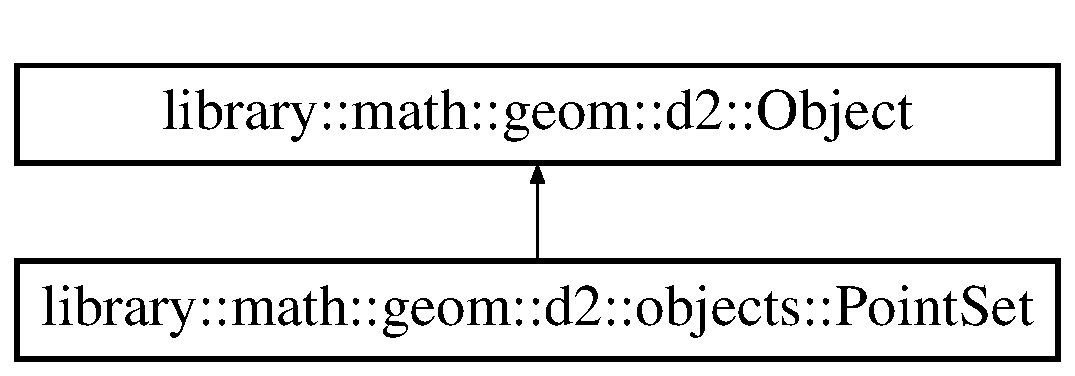
\includegraphics[height=2.000000cm]{classlibrary_1_1math_1_1geom_1_1d2_1_1objects_1_1_point_set}
\end{center}
\end{figure}
\subsection*{Classes}
\begin{DoxyCompactItemize}
\item 
struct \hyperlink{structlibrary_1_1math_1_1geom_1_1d2_1_1objects_1_1_point_set_1_1_hasher}{Hasher}
\begin{DoxyCompactList}\small\item\em \hyperlink{classlibrary_1_1math_1_1geom_1_1d2_1_1objects_1_1_point}{Point} hasher. \end{DoxyCompactList}\end{DoxyCompactItemize}
\subsection*{Public Types}
\begin{DoxyCompactItemize}
\item 
typedef std\+::unordered\+\_\+set$<$ \hyperlink{classlibrary_1_1math_1_1geom_1_1d2_1_1objects_1_1_point}{Point}, \hyperlink{structlibrary_1_1math_1_1geom_1_1d2_1_1objects_1_1_point_set_1_1_hasher}{Point\+Set\+::\+Hasher} $>$ \hyperlink{classlibrary_1_1math_1_1geom_1_1d2_1_1objects_1_1_point_set_a4ad340e72ff6c1a80199804754cd1af9}{Container}
\item 
typedef Point\+Set\+::\+Container\+::const\+\_\+iterator \hyperlink{classlibrary_1_1math_1_1geom_1_1d2_1_1objects_1_1_point_set_ad4c4f52fdc966f0d2031402edefc9e98}{Const\+Iterator}
\end{DoxyCompactItemize}
\subsection*{Public Member Functions}
\begin{DoxyCompactItemize}
\item 
\hyperlink{classlibrary_1_1math_1_1geom_1_1d2_1_1objects_1_1_point_set_a1b27139683b5b3418188e3eae1385618}{Point\+Set} (const Array$<$ \hyperlink{classlibrary_1_1math_1_1geom_1_1d2_1_1objects_1_1_point}{Point} $>$ \&a\+Point\+Array)
\begin{DoxyCompactList}\small\item\em Constructor. \end{DoxyCompactList}\item 
virtual \hyperlink{classlibrary_1_1math_1_1geom_1_1d2_1_1objects_1_1_point_set}{Point\+Set} $\ast$ \hyperlink{classlibrary_1_1math_1_1geom_1_1d2_1_1objects_1_1_point_set_ad867c4fb86734efe968a39c95eba53b3}{clone} () const override
\begin{DoxyCompactList}\small\item\em Clone point set. \end{DoxyCompactList}\item 
bool \hyperlink{classlibrary_1_1math_1_1geom_1_1d2_1_1objects_1_1_point_set_a0e0187a6f35dadf000b69615b9b82cde}{operator==} (const \hyperlink{classlibrary_1_1math_1_1geom_1_1d2_1_1objects_1_1_point_set}{Point\+Set} \&a\+Point\+Set) const
\begin{DoxyCompactList}\small\item\em Equal to operator. \end{DoxyCompactList}\item 
bool \hyperlink{classlibrary_1_1math_1_1geom_1_1d2_1_1objects_1_1_point_set_a5c03cc2e46ae682725291ae02c5063cf}{operator!=} (const \hyperlink{classlibrary_1_1math_1_1geom_1_1d2_1_1objects_1_1_point_set}{Point\+Set} \&a\+Point\+Set) const
\begin{DoxyCompactList}\small\item\em Not equal to operator. \end{DoxyCompactList}\item 
virtual bool \hyperlink{classlibrary_1_1math_1_1geom_1_1d2_1_1objects_1_1_point_set_a031a6b5688c65bce8f37af452c0f0959}{is\+Defined} () const override
\begin{DoxyCompactList}\small\item\em Check if point set is defined. \end{DoxyCompactList}\item 
bool \hyperlink{classlibrary_1_1math_1_1geom_1_1d2_1_1objects_1_1_point_set_af81b5c7b407db5fc7021f71ab10497ea}{is\+Empty} () const
\begin{DoxyCompactList}\small\item\em Check if point set is empty. \end{DoxyCompactList}\item 
bool \hyperlink{classlibrary_1_1math_1_1geom_1_1d2_1_1objects_1_1_point_set_a8aba7c99e93720ba291abef2ded25cc7}{is\+Near} (const \hyperlink{classlibrary_1_1math_1_1geom_1_1d2_1_1objects_1_1_point_set}{Point\+Set} \&a\+Point\+Set, const Real \&a\+Tolerance) const
\begin{DoxyCompactList}\small\item\em Check if point set is near another point set. \end{DoxyCompactList}\item 
Size \hyperlink{classlibrary_1_1math_1_1geom_1_1d2_1_1objects_1_1_point_set_a7a0cfe0925906d863e0e89605344838d}{get\+Size} () const
\begin{DoxyCompactList}\small\item\em Get size of point set. \end{DoxyCompactList}\item 
\hyperlink{classlibrary_1_1math_1_1geom_1_1d2_1_1objects_1_1_point}{Point} \hyperlink{classlibrary_1_1math_1_1geom_1_1d2_1_1objects_1_1_point_set_a4d4944b034ead53d1b734fe74cd1bc60}{get\+Point\+Closest\+To} (const \hyperlink{classlibrary_1_1math_1_1geom_1_1d2_1_1objects_1_1_point}{Point} \&a\+Point) const
\begin{DoxyCompactList}\small\item\em Get point closest to another point. \end{DoxyCompactList}\item 
virtual String \hyperlink{classlibrary_1_1math_1_1geom_1_1d2_1_1objects_1_1_point_set_a4eeece63192481627cb0f991a4eef1a4}{to\+String} (const \hyperlink{classlibrary_1_1math_1_1geom_1_1d2_1_1_object_ac8cd61dada4960cfee9a469231621b17}{Object\+::\+Format} \&a\+Format=\hyperlink{classlibrary_1_1math_1_1geom_1_1d2_1_1_object_ac8cd61dada4960cfee9a469231621b17aeb6d8ae6f20283755b339c0dc273988b}{Object\+::\+Format\+::\+Standard}, const Integer \&a\+Precision=Integer\+::\+Undefined()) const override
\begin{DoxyCompactList}\small\item\em Get string representation. \end{DoxyCompactList}\item 
virtual void \hyperlink{classlibrary_1_1math_1_1geom_1_1d2_1_1objects_1_1_point_set_a652098938854c19294b5df8e8634cc9a}{print} (std\+::ostream \&an\+Output\+Stream, bool display\+Decorators=true) const override
\begin{DoxyCompactList}\small\item\em Print point. \end{DoxyCompactList}\item 
\hyperlink{classlibrary_1_1math_1_1geom_1_1d2_1_1objects_1_1_point_set_ad4c4f52fdc966f0d2031402edefc9e98}{Point\+Set\+::\+Const\+Iterator} \hyperlink{classlibrary_1_1math_1_1geom_1_1d2_1_1objects_1_1_point_set_ae7e4ce8100cde825aa0d3c5cc092eef9}{begin} () const
\begin{DoxyCompactList}\small\item\em Get begin const iterator. \end{DoxyCompactList}\item 
\hyperlink{classlibrary_1_1math_1_1geom_1_1d2_1_1objects_1_1_point_set_ad4c4f52fdc966f0d2031402edefc9e98}{Point\+Set\+::\+Const\+Iterator} \hyperlink{classlibrary_1_1math_1_1geom_1_1d2_1_1objects_1_1_point_set_a7ae46d64848d5dda85ea621bb0f24ef7}{end} () const
\begin{DoxyCompactList}\small\item\em Get end const iterator. \end{DoxyCompactList}\item 
virtual void \hyperlink{classlibrary_1_1math_1_1geom_1_1d2_1_1objects_1_1_point_set_acfb8652fd1f17f101e7750a0b81452c0}{apply\+Transformation} (const \hyperlink{classlibrary_1_1math_1_1geom_1_1d2_1_1_transformation}{Transformation} \&a\+Transformation) override
\begin{DoxyCompactList}\small\item\em Apply transformation to point set. \end{DoxyCompactList}\end{DoxyCompactItemize}
\subsection*{Static Public Member Functions}
\begin{DoxyCompactItemize}
\item 
static \hyperlink{classlibrary_1_1math_1_1geom_1_1d2_1_1objects_1_1_point_set}{Point\+Set} \hyperlink{classlibrary_1_1math_1_1geom_1_1d2_1_1objects_1_1_point_set_af09fa6d8bce9f64b150c739e1ed7bfc6}{Empty} ()
\begin{DoxyCompactList}\small\item\em Constructs an empty point set. \end{DoxyCompactList}\end{DoxyCompactItemize}


\subsection{Detailed Description}
\hyperlink{classlibrary_1_1math_1_1geom_1_1d2_1_1objects_1_1_point}{Point} set. 

\subsection{Member Typedef Documentation}
\mbox{\Hypertarget{classlibrary_1_1math_1_1geom_1_1d2_1_1objects_1_1_point_set_ad4c4f52fdc966f0d2031402edefc9e98}\label{classlibrary_1_1math_1_1geom_1_1d2_1_1objects_1_1_point_set_ad4c4f52fdc966f0d2031402edefc9e98}} 
\index{library\+::math\+::geom\+::d2\+::objects\+::\+Point\+Set@{library\+::math\+::geom\+::d2\+::objects\+::\+Point\+Set}!Const\+Iterator@{Const\+Iterator}}
\index{Const\+Iterator@{Const\+Iterator}!library\+::math\+::geom\+::d2\+::objects\+::\+Point\+Set@{library\+::math\+::geom\+::d2\+::objects\+::\+Point\+Set}}
\subsubsection{\texorpdfstring{Const\+Iterator}{ConstIterator}}
{\footnotesize\ttfamily typedef Point\+Set\+::\+Container\+::const\+\_\+iterator \hyperlink{classlibrary_1_1math_1_1geom_1_1d2_1_1objects_1_1_point_set_ad4c4f52fdc966f0d2031402edefc9e98}{library\+::math\+::geom\+::d2\+::objects\+::\+Point\+Set\+::\+Const\+Iterator}}

\mbox{\Hypertarget{classlibrary_1_1math_1_1geom_1_1d2_1_1objects_1_1_point_set_a4ad340e72ff6c1a80199804754cd1af9}\label{classlibrary_1_1math_1_1geom_1_1d2_1_1objects_1_1_point_set_a4ad340e72ff6c1a80199804754cd1af9}} 
\index{library\+::math\+::geom\+::d2\+::objects\+::\+Point\+Set@{library\+::math\+::geom\+::d2\+::objects\+::\+Point\+Set}!Container@{Container}}
\index{Container@{Container}!library\+::math\+::geom\+::d2\+::objects\+::\+Point\+Set@{library\+::math\+::geom\+::d2\+::objects\+::\+Point\+Set}}
\subsubsection{\texorpdfstring{Container}{Container}}
{\footnotesize\ttfamily typedef std\+::unordered\+\_\+set$<$\hyperlink{classlibrary_1_1math_1_1geom_1_1d2_1_1objects_1_1_point}{Point}, \hyperlink{structlibrary_1_1math_1_1geom_1_1d2_1_1objects_1_1_point_set_1_1_hasher}{Point\+Set\+::\+Hasher}$>$ \hyperlink{classlibrary_1_1math_1_1geom_1_1d2_1_1objects_1_1_point_set_a4ad340e72ff6c1a80199804754cd1af9}{library\+::math\+::geom\+::d2\+::objects\+::\+Point\+Set\+::\+Container}}



\subsection{Constructor \& Destructor Documentation}
\mbox{\Hypertarget{classlibrary_1_1math_1_1geom_1_1d2_1_1objects_1_1_point_set_a1b27139683b5b3418188e3eae1385618}\label{classlibrary_1_1math_1_1geom_1_1d2_1_1objects_1_1_point_set_a1b27139683b5b3418188e3eae1385618}} 
\index{library\+::math\+::geom\+::d2\+::objects\+::\+Point\+Set@{library\+::math\+::geom\+::d2\+::objects\+::\+Point\+Set}!Point\+Set@{Point\+Set}}
\index{Point\+Set@{Point\+Set}!library\+::math\+::geom\+::d2\+::objects\+::\+Point\+Set@{library\+::math\+::geom\+::d2\+::objects\+::\+Point\+Set}}
\subsubsection{\texorpdfstring{Point\+Set()}{PointSet()}}
{\footnotesize\ttfamily library\+::math\+::geom\+::d2\+::objects\+::\+Point\+Set\+::\+Point\+Set (\begin{DoxyParamCaption}\item[{const Array$<$ \hyperlink{classlibrary_1_1math_1_1geom_1_1d2_1_1objects_1_1_point}{Point} $>$ \&}]{a\+Point\+Array }\end{DoxyParamCaption})}



Constructor. 


\begin{DoxyCode}
\hyperlink{classlibrary_1_1math_1_1geom_1_1d2_1_1objects_1_1_point_set_a1b27139683b5b3418188e3eae1385618}{PointSet} pointSet(\{ \{ 0.0, 0.0 \}, \{ 0.0, 1.0 \} \}) ;
\end{DoxyCode}



\begin{DoxyParams}[1]{Parameters}
\mbox{\tt in}  & {\em a\+Point\+Array} & A point array \\
\hline
\end{DoxyParams}


\subsection{Member Function Documentation}
\mbox{\Hypertarget{classlibrary_1_1math_1_1geom_1_1d2_1_1objects_1_1_point_set_acfb8652fd1f17f101e7750a0b81452c0}\label{classlibrary_1_1math_1_1geom_1_1d2_1_1objects_1_1_point_set_acfb8652fd1f17f101e7750a0b81452c0}} 
\index{library\+::math\+::geom\+::d2\+::objects\+::\+Point\+Set@{library\+::math\+::geom\+::d2\+::objects\+::\+Point\+Set}!apply\+Transformation@{apply\+Transformation}}
\index{apply\+Transformation@{apply\+Transformation}!library\+::math\+::geom\+::d2\+::objects\+::\+Point\+Set@{library\+::math\+::geom\+::d2\+::objects\+::\+Point\+Set}}
\subsubsection{\texorpdfstring{apply\+Transformation()}{applyTransformation()}}
{\footnotesize\ttfamily void library\+::math\+::geom\+::d2\+::objects\+::\+Point\+Set\+::apply\+Transformation (\begin{DoxyParamCaption}\item[{const \hyperlink{classlibrary_1_1math_1_1geom_1_1d2_1_1_transformation}{Transformation} \&}]{a\+Transformation }\end{DoxyParamCaption})\hspace{0.3cm}{\ttfamily [override]}, {\ttfamily [virtual]}}



Apply transformation to point set. 


\begin{DoxyParams}[1]{Parameters}
\mbox{\tt in}  & {\em a\+Transformation} & A transformation \\
\hline
\end{DoxyParams}


Implements \hyperlink{classlibrary_1_1math_1_1geom_1_1d2_1_1_object_a289589fb6e9e7a2c4ca4976a1544def5}{library\+::math\+::geom\+::d2\+::\+Object}.

\mbox{\Hypertarget{classlibrary_1_1math_1_1geom_1_1d2_1_1objects_1_1_point_set_ae7e4ce8100cde825aa0d3c5cc092eef9}\label{classlibrary_1_1math_1_1geom_1_1d2_1_1objects_1_1_point_set_ae7e4ce8100cde825aa0d3c5cc092eef9}} 
\index{library\+::math\+::geom\+::d2\+::objects\+::\+Point\+Set@{library\+::math\+::geom\+::d2\+::objects\+::\+Point\+Set}!begin@{begin}}
\index{begin@{begin}!library\+::math\+::geom\+::d2\+::objects\+::\+Point\+Set@{library\+::math\+::geom\+::d2\+::objects\+::\+Point\+Set}}
\subsubsection{\texorpdfstring{begin()}{begin()}}
{\footnotesize\ttfamily \hyperlink{classlibrary_1_1math_1_1geom_1_1d2_1_1objects_1_1_point_set_ad4c4f52fdc966f0d2031402edefc9e98}{Point\+Set\+::\+Const\+Iterator} library\+::math\+::geom\+::d2\+::objects\+::\+Point\+Set\+::begin (\begin{DoxyParamCaption}{ }\end{DoxyParamCaption}) const}



Get begin const iterator. 

\begin{DoxyReturn}{Returns}
Begin const iterator 
\end{DoxyReturn}
\mbox{\Hypertarget{classlibrary_1_1math_1_1geom_1_1d2_1_1objects_1_1_point_set_ad867c4fb86734efe968a39c95eba53b3}\label{classlibrary_1_1math_1_1geom_1_1d2_1_1objects_1_1_point_set_ad867c4fb86734efe968a39c95eba53b3}} 
\index{library\+::math\+::geom\+::d2\+::objects\+::\+Point\+Set@{library\+::math\+::geom\+::d2\+::objects\+::\+Point\+Set}!clone@{clone}}
\index{clone@{clone}!library\+::math\+::geom\+::d2\+::objects\+::\+Point\+Set@{library\+::math\+::geom\+::d2\+::objects\+::\+Point\+Set}}
\subsubsection{\texorpdfstring{clone()}{clone()}}
{\footnotesize\ttfamily \hyperlink{classlibrary_1_1math_1_1geom_1_1d2_1_1objects_1_1_point_set}{Point\+Set} $\ast$ library\+::math\+::geom\+::d2\+::objects\+::\+Point\+Set\+::clone (\begin{DoxyParamCaption}{ }\end{DoxyParamCaption}) const\hspace{0.3cm}{\ttfamily [override]}, {\ttfamily [virtual]}}



Clone point set. 

\begin{DoxyReturn}{Returns}
Pointer to cloned point set 
\end{DoxyReturn}


Implements \hyperlink{classlibrary_1_1math_1_1geom_1_1d2_1_1_object_a5c26ae4120edb24f6463d65a9cef247d}{library\+::math\+::geom\+::d2\+::\+Object}.

\mbox{\Hypertarget{classlibrary_1_1math_1_1geom_1_1d2_1_1objects_1_1_point_set_af09fa6d8bce9f64b150c739e1ed7bfc6}\label{classlibrary_1_1math_1_1geom_1_1d2_1_1objects_1_1_point_set_af09fa6d8bce9f64b150c739e1ed7bfc6}} 
\index{library\+::math\+::geom\+::d2\+::objects\+::\+Point\+Set@{library\+::math\+::geom\+::d2\+::objects\+::\+Point\+Set}!Empty@{Empty}}
\index{Empty@{Empty}!library\+::math\+::geom\+::d2\+::objects\+::\+Point\+Set@{library\+::math\+::geom\+::d2\+::objects\+::\+Point\+Set}}
\subsubsection{\texorpdfstring{Empty()}{Empty()}}
{\footnotesize\ttfamily \hyperlink{classlibrary_1_1math_1_1geom_1_1d2_1_1objects_1_1_point_set}{Point\+Set} library\+::math\+::geom\+::d2\+::objects\+::\+Point\+Set\+::\+Empty (\begin{DoxyParamCaption}{ }\end{DoxyParamCaption})\hspace{0.3cm}{\ttfamily [static]}}



Constructs an empty point set. 


\begin{DoxyCode}
\hyperlink{classlibrary_1_1math_1_1geom_1_1d2_1_1objects_1_1_point_set_a1b27139683b5b3418188e3eae1385618}{PointSet} pointSet = \hyperlink{classlibrary_1_1math_1_1geom_1_1d2_1_1objects_1_1_point_set_af09fa6d8bce9f64b150c739e1ed7bfc6}{PointSet::Empty}() ;
\end{DoxyCode}


\begin{DoxyReturn}{Returns}
Empty point set 
\end{DoxyReturn}
\mbox{\Hypertarget{classlibrary_1_1math_1_1geom_1_1d2_1_1objects_1_1_point_set_a7ae46d64848d5dda85ea621bb0f24ef7}\label{classlibrary_1_1math_1_1geom_1_1d2_1_1objects_1_1_point_set_a7ae46d64848d5dda85ea621bb0f24ef7}} 
\index{library\+::math\+::geom\+::d2\+::objects\+::\+Point\+Set@{library\+::math\+::geom\+::d2\+::objects\+::\+Point\+Set}!end@{end}}
\index{end@{end}!library\+::math\+::geom\+::d2\+::objects\+::\+Point\+Set@{library\+::math\+::geom\+::d2\+::objects\+::\+Point\+Set}}
\subsubsection{\texorpdfstring{end()}{end()}}
{\footnotesize\ttfamily \hyperlink{classlibrary_1_1math_1_1geom_1_1d2_1_1objects_1_1_point_set_ad4c4f52fdc966f0d2031402edefc9e98}{Point\+Set\+::\+Const\+Iterator} library\+::math\+::geom\+::d2\+::objects\+::\+Point\+Set\+::end (\begin{DoxyParamCaption}{ }\end{DoxyParamCaption}) const}



Get end const iterator. 

\begin{DoxyReturn}{Returns}
End const iterator 
\end{DoxyReturn}
\mbox{\Hypertarget{classlibrary_1_1math_1_1geom_1_1d2_1_1objects_1_1_point_set_a4d4944b034ead53d1b734fe74cd1bc60}\label{classlibrary_1_1math_1_1geom_1_1d2_1_1objects_1_1_point_set_a4d4944b034ead53d1b734fe74cd1bc60}} 
\index{library\+::math\+::geom\+::d2\+::objects\+::\+Point\+Set@{library\+::math\+::geom\+::d2\+::objects\+::\+Point\+Set}!get\+Point\+Closest\+To@{get\+Point\+Closest\+To}}
\index{get\+Point\+Closest\+To@{get\+Point\+Closest\+To}!library\+::math\+::geom\+::d2\+::objects\+::\+Point\+Set@{library\+::math\+::geom\+::d2\+::objects\+::\+Point\+Set}}
\subsubsection{\texorpdfstring{get\+Point\+Closest\+To()}{getPointClosestTo()}}
{\footnotesize\ttfamily \hyperlink{classlibrary_1_1math_1_1geom_1_1d2_1_1objects_1_1_point}{Point} library\+::math\+::geom\+::d2\+::objects\+::\+Point\+Set\+::get\+Point\+Closest\+To (\begin{DoxyParamCaption}\item[{const \hyperlink{classlibrary_1_1math_1_1geom_1_1d2_1_1objects_1_1_point}{Point} \&}]{a\+Point }\end{DoxyParamCaption}) const}



Get point closest to another point. 


\begin{DoxyParams}[1]{Parameters}
\mbox{\tt in}  & {\em a\+Point} & A point \\
\hline
\end{DoxyParams}
\begin{DoxyReturn}{Returns}
Closest point 
\end{DoxyReturn}
\mbox{\Hypertarget{classlibrary_1_1math_1_1geom_1_1d2_1_1objects_1_1_point_set_a7a0cfe0925906d863e0e89605344838d}\label{classlibrary_1_1math_1_1geom_1_1d2_1_1objects_1_1_point_set_a7a0cfe0925906d863e0e89605344838d}} 
\index{library\+::math\+::geom\+::d2\+::objects\+::\+Point\+Set@{library\+::math\+::geom\+::d2\+::objects\+::\+Point\+Set}!get\+Size@{get\+Size}}
\index{get\+Size@{get\+Size}!library\+::math\+::geom\+::d2\+::objects\+::\+Point\+Set@{library\+::math\+::geom\+::d2\+::objects\+::\+Point\+Set}}
\subsubsection{\texorpdfstring{get\+Size()}{getSize()}}
{\footnotesize\ttfamily Size library\+::math\+::geom\+::d2\+::objects\+::\+Point\+Set\+::get\+Size (\begin{DoxyParamCaption}{ }\end{DoxyParamCaption}) const}



Get size of point set. 

\begin{DoxyReturn}{Returns}
Size of point set 
\end{DoxyReturn}
\mbox{\Hypertarget{classlibrary_1_1math_1_1geom_1_1d2_1_1objects_1_1_point_set_a031a6b5688c65bce8f37af452c0f0959}\label{classlibrary_1_1math_1_1geom_1_1d2_1_1objects_1_1_point_set_a031a6b5688c65bce8f37af452c0f0959}} 
\index{library\+::math\+::geom\+::d2\+::objects\+::\+Point\+Set@{library\+::math\+::geom\+::d2\+::objects\+::\+Point\+Set}!is\+Defined@{is\+Defined}}
\index{is\+Defined@{is\+Defined}!library\+::math\+::geom\+::d2\+::objects\+::\+Point\+Set@{library\+::math\+::geom\+::d2\+::objects\+::\+Point\+Set}}
\subsubsection{\texorpdfstring{is\+Defined()}{isDefined()}}
{\footnotesize\ttfamily bool library\+::math\+::geom\+::d2\+::objects\+::\+Point\+Set\+::is\+Defined (\begin{DoxyParamCaption}{ }\end{DoxyParamCaption}) const\hspace{0.3cm}{\ttfamily [override]}, {\ttfamily [virtual]}}



Check if point set is defined. 


\begin{DoxyCode}
\hyperlink{classlibrary_1_1math_1_1geom_1_1d2_1_1objects_1_1_point_set_a1b27139683b5b3418188e3eae1385618}{PointSet}(0.0, 0.0).isDefined() ; \textcolor{comment}{// True}
\end{DoxyCode}


\begin{DoxyReturn}{Returns}
True if point set is defined 
\end{DoxyReturn}


Implements \hyperlink{classlibrary_1_1math_1_1geom_1_1d2_1_1_object_ae9506254971168a3ca63e1923556b70d}{library\+::math\+::geom\+::d2\+::\+Object}.

\mbox{\Hypertarget{classlibrary_1_1math_1_1geom_1_1d2_1_1objects_1_1_point_set_af81b5c7b407db5fc7021f71ab10497ea}\label{classlibrary_1_1math_1_1geom_1_1d2_1_1objects_1_1_point_set_af81b5c7b407db5fc7021f71ab10497ea}} 
\index{library\+::math\+::geom\+::d2\+::objects\+::\+Point\+Set@{library\+::math\+::geom\+::d2\+::objects\+::\+Point\+Set}!is\+Empty@{is\+Empty}}
\index{is\+Empty@{is\+Empty}!library\+::math\+::geom\+::d2\+::objects\+::\+Point\+Set@{library\+::math\+::geom\+::d2\+::objects\+::\+Point\+Set}}
\subsubsection{\texorpdfstring{is\+Empty()}{isEmpty()}}
{\footnotesize\ttfamily bool library\+::math\+::geom\+::d2\+::objects\+::\+Point\+Set\+::is\+Empty (\begin{DoxyParamCaption}{ }\end{DoxyParamCaption}) const}



Check if point set is empty. 


\begin{DoxyCode}
\hyperlink{classlibrary_1_1math_1_1geom_1_1d2_1_1objects_1_1_point_set_af09fa6d8bce9f64b150c739e1ed7bfc6}{PointSet::Empty}().\hyperlink{classlibrary_1_1math_1_1geom_1_1d2_1_1objects_1_1_point_set_af81b5c7b407db5fc7021f71ab10497ea}{isEmpty}() ; \textcolor{comment}{// True}
\end{DoxyCode}


\begin{DoxyReturn}{Returns}
True if point set is empty 
\end{DoxyReturn}
\mbox{\Hypertarget{classlibrary_1_1math_1_1geom_1_1d2_1_1objects_1_1_point_set_a8aba7c99e93720ba291abef2ded25cc7}\label{classlibrary_1_1math_1_1geom_1_1d2_1_1objects_1_1_point_set_a8aba7c99e93720ba291abef2ded25cc7}} 
\index{library\+::math\+::geom\+::d2\+::objects\+::\+Point\+Set@{library\+::math\+::geom\+::d2\+::objects\+::\+Point\+Set}!is\+Near@{is\+Near}}
\index{is\+Near@{is\+Near}!library\+::math\+::geom\+::d2\+::objects\+::\+Point\+Set@{library\+::math\+::geom\+::d2\+::objects\+::\+Point\+Set}}
\subsubsection{\texorpdfstring{is\+Near()}{isNear()}}
{\footnotesize\ttfamily bool library\+::math\+::geom\+::d2\+::objects\+::\+Point\+Set\+::is\+Near (\begin{DoxyParamCaption}\item[{const \hyperlink{classlibrary_1_1math_1_1geom_1_1d2_1_1objects_1_1_point_set}{Point\+Set} \&}]{a\+Point\+Set,  }\item[{const Real \&}]{a\+Tolerance }\end{DoxyParamCaption}) const}



Check if point set is near another point set. 


\begin{DoxyCode}
\hyperlink{classlibrary_1_1math_1_1geom_1_1d2_1_1objects_1_1_point_set_a1b27139683b5b3418188e3eae1385618}{PointSet}(\{ \{ 0.0, 0.0 \}, \{ 0.0, 1.0 \} \}).\hyperlink{classlibrary_1_1math_1_1geom_1_1d2_1_1objects_1_1_point_set_a8aba7c99e93720ba291abef2ded25cc7}{isNear}(\hyperlink{classlibrary_1_1math_1_1geom_1_1d2_1_1objects_1_1_point_set_a1b27139683b5b3418188e3eae1385618}{PointSet}(\{ \{ 0.0, 1e-15 \}, \{ 0.0, 1.0
       \} \}), 1e-15) ; \textcolor{comment}{// True}
\end{DoxyCode}



\begin{DoxyParams}[1]{Parameters}
\mbox{\tt in}  & {\em a\+Point\+Set} & A point set \\
\hline
\mbox{\tt in}  & {\em a\+Tolerance} & A tolerance \\
\hline
\end{DoxyParams}
\begin{DoxyReturn}{Returns}
True if point set is near another point set 
\end{DoxyReturn}
\mbox{\Hypertarget{classlibrary_1_1math_1_1geom_1_1d2_1_1objects_1_1_point_set_a5c03cc2e46ae682725291ae02c5063cf}\label{classlibrary_1_1math_1_1geom_1_1d2_1_1objects_1_1_point_set_a5c03cc2e46ae682725291ae02c5063cf}} 
\index{library\+::math\+::geom\+::d2\+::objects\+::\+Point\+Set@{library\+::math\+::geom\+::d2\+::objects\+::\+Point\+Set}!operator"!=@{operator"!=}}
\index{operator"!=@{operator"!=}!library\+::math\+::geom\+::d2\+::objects\+::\+Point\+Set@{library\+::math\+::geom\+::d2\+::objects\+::\+Point\+Set}}
\subsubsection{\texorpdfstring{operator"!=()}{operator!=()}}
{\footnotesize\ttfamily bool library\+::math\+::geom\+::d2\+::objects\+::\+Point\+Set\+::operator!= (\begin{DoxyParamCaption}\item[{const \hyperlink{classlibrary_1_1math_1_1geom_1_1d2_1_1objects_1_1_point_set}{Point\+Set} \&}]{a\+Point\+Set }\end{DoxyParamCaption}) const}



Not equal to operator. 


\begin{DoxyParams}[1]{Parameters}
\mbox{\tt in}  & {\em a\+Point\+Set} & A point set \\
\hline
\end{DoxyParams}
\begin{DoxyReturn}{Returns}
True if point sets not are equal 
\end{DoxyReturn}
\mbox{\Hypertarget{classlibrary_1_1math_1_1geom_1_1d2_1_1objects_1_1_point_set_a0e0187a6f35dadf000b69615b9b82cde}\label{classlibrary_1_1math_1_1geom_1_1d2_1_1objects_1_1_point_set_a0e0187a6f35dadf000b69615b9b82cde}} 
\index{library\+::math\+::geom\+::d2\+::objects\+::\+Point\+Set@{library\+::math\+::geom\+::d2\+::objects\+::\+Point\+Set}!operator==@{operator==}}
\index{operator==@{operator==}!library\+::math\+::geom\+::d2\+::objects\+::\+Point\+Set@{library\+::math\+::geom\+::d2\+::objects\+::\+Point\+Set}}
\subsubsection{\texorpdfstring{operator==()}{operator==()}}
{\footnotesize\ttfamily bool library\+::math\+::geom\+::d2\+::objects\+::\+Point\+Set\+::operator== (\begin{DoxyParamCaption}\item[{const \hyperlink{classlibrary_1_1math_1_1geom_1_1d2_1_1objects_1_1_point_set}{Point\+Set} \&}]{a\+Point\+Set }\end{DoxyParamCaption}) const}



Equal to operator. 


\begin{DoxyParams}[1]{Parameters}
\mbox{\tt in}  & {\em a\+Point\+Set} & A point set \\
\hline
\end{DoxyParams}
\begin{DoxyReturn}{Returns}
True if point sets are equal 
\end{DoxyReturn}
\mbox{\Hypertarget{classlibrary_1_1math_1_1geom_1_1d2_1_1objects_1_1_point_set_a652098938854c19294b5df8e8634cc9a}\label{classlibrary_1_1math_1_1geom_1_1d2_1_1objects_1_1_point_set_a652098938854c19294b5df8e8634cc9a}} 
\index{library\+::math\+::geom\+::d2\+::objects\+::\+Point\+Set@{library\+::math\+::geom\+::d2\+::objects\+::\+Point\+Set}!print@{print}}
\index{print@{print}!library\+::math\+::geom\+::d2\+::objects\+::\+Point\+Set@{library\+::math\+::geom\+::d2\+::objects\+::\+Point\+Set}}
\subsubsection{\texorpdfstring{print()}{print()}}
{\footnotesize\ttfamily void library\+::math\+::geom\+::d2\+::objects\+::\+Point\+Set\+::print (\begin{DoxyParamCaption}\item[{std\+::ostream \&}]{an\+Output\+Stream,  }\item[{bool}]{display\+Decorators = {\ttfamily true} }\end{DoxyParamCaption}) const\hspace{0.3cm}{\ttfamily [override]}, {\ttfamily [virtual]}}



Print point. 


\begin{DoxyParams}[1]{Parameters}
\mbox{\tt in}  & {\em an\+Output\+Stream} & An output stream \\
\hline
\mbox{\tt in}  & {\em (optional)} & display\+Decorators If true, display decorators \\
\hline
\end{DoxyParams}


Implements \hyperlink{classlibrary_1_1math_1_1geom_1_1d2_1_1_object_a834bbf59cf1c483d1dc7b0966b1e1ab3}{library\+::math\+::geom\+::d2\+::\+Object}.

\mbox{\Hypertarget{classlibrary_1_1math_1_1geom_1_1d2_1_1objects_1_1_point_set_a4eeece63192481627cb0f991a4eef1a4}\label{classlibrary_1_1math_1_1geom_1_1d2_1_1objects_1_1_point_set_a4eeece63192481627cb0f991a4eef1a4}} 
\index{library\+::math\+::geom\+::d2\+::objects\+::\+Point\+Set@{library\+::math\+::geom\+::d2\+::objects\+::\+Point\+Set}!to\+String@{to\+String}}
\index{to\+String@{to\+String}!library\+::math\+::geom\+::d2\+::objects\+::\+Point\+Set@{library\+::math\+::geom\+::d2\+::objects\+::\+Point\+Set}}
\subsubsection{\texorpdfstring{to\+String()}{toString()}}
{\footnotesize\ttfamily String library\+::math\+::geom\+::d2\+::objects\+::\+Point\+Set\+::to\+String (\begin{DoxyParamCaption}\item[{const \hyperlink{classlibrary_1_1math_1_1geom_1_1d2_1_1_object_ac8cd61dada4960cfee9a469231621b17}{Object\+::\+Format} \&}]{a\+Format = {\ttfamily \hyperlink{classlibrary_1_1math_1_1geom_1_1d2_1_1_object_ac8cd61dada4960cfee9a469231621b17aeb6d8ae6f20283755b339c0dc273988b}{Object\+::\+Format\+::\+Standard}},  }\item[{const Integer \&}]{a\+Precision = {\ttfamily Integer\+:\+:Undefined()} }\end{DoxyParamCaption}) const\hspace{0.3cm}{\ttfamily [override]}, {\ttfamily [virtual]}}



Get string representation. 


\begin{DoxyParams}[1]{Parameters}
\mbox{\tt in}  & {\em a\+Format} & A format \\
\hline
\end{DoxyParams}
\begin{DoxyReturn}{Returns}
String representation 
\end{DoxyReturn}


Implements \hyperlink{classlibrary_1_1math_1_1geom_1_1d2_1_1_object_acdd76b3637732a249536b609dbe3f0eb}{library\+::math\+::geom\+::d2\+::\+Object}.



The documentation for this class was generated from the following files\+:\begin{DoxyCompactItemize}
\item 
include/\+Library/\+Mathematics/\+Geometry/2\+D/\+Objects/\hyperlink{2_d_2_objects_2_point_set_8hpp}{Point\+Set.\+hpp}\item 
src/\+Library/\+Mathematics/\+Geometry/2\+D/\+Objects/\hyperlink{2_d_2_objects_2_point_set_8cpp}{Point\+Set.\+cpp}\end{DoxyCompactItemize}

\hypertarget{classlibrary_1_1math_1_1geom_1_1d2_1_1objects_1_1_polygon}{}\section{library\+:\+:math\+:\+:geom\+:\+:d2\+:\+:objects\+:\+:Polygon Class Reference}
\label{classlibrary_1_1math_1_1geom_1_1d2_1_1objects_1_1_polygon}\index{library\+::math\+::geom\+::d2\+::objects\+::\+Polygon@{library\+::math\+::geom\+::d2\+::objects\+::\+Polygon}}


\hyperlink{classlibrary_1_1math_1_1geom_1_1d2_1_1objects_1_1_polygon}{Polygon}.  




{\ttfamily \#include $<$Polygon.\+hpp$>$}

Inheritance diagram for library\+:\+:math\+:\+:geom\+:\+:d2\+:\+:objects\+:\+:Polygon\+:\begin{figure}[H]
\begin{center}
\leavevmode
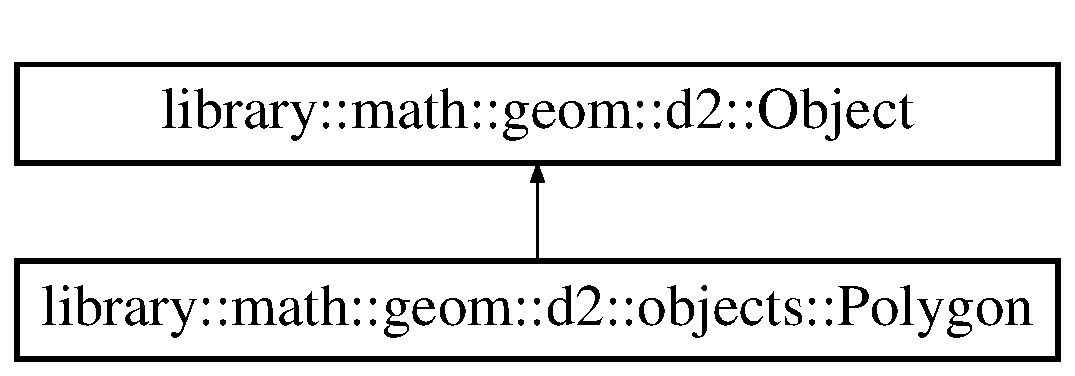
\includegraphics[height=2.000000cm]{classlibrary_1_1math_1_1geom_1_1d2_1_1objects_1_1_polygon}
\end{center}
\end{figure}
\subsection*{Public Member Functions}
\begin{DoxyCompactItemize}
\item 
\hyperlink{classlibrary_1_1math_1_1geom_1_1d2_1_1objects_1_1_polygon_ad2a0b0bcd5301dbcd9e2fa101fbd220b}{Polygon} (const Array$<$ \hyperlink{classlibrary_1_1math_1_1geom_1_1d2_1_1objects_1_1_point}{Point} $>$ \&an\+Outer\+Ring, const Array$<$ Array$<$ \hyperlink{classlibrary_1_1math_1_1geom_1_1d2_1_1objects_1_1_point}{Point} $>$$>$ \&an\+Inner\+Ring\+Array=Array$<$ Array$<$ \hyperlink{classlibrary_1_1math_1_1geom_1_1d2_1_1objects_1_1_point}{Point} $>$$>$\+::Empty())
\begin{DoxyCompactList}\small\item\em Constructor. \end{DoxyCompactList}\item 
\hyperlink{classlibrary_1_1math_1_1geom_1_1d2_1_1objects_1_1_polygon_a6384fadfb81c792d137693e8f0dd14f9}{Polygon} (const \hyperlink{classlibrary_1_1math_1_1geom_1_1d2_1_1objects_1_1_polygon}{Polygon} \&a\+Polygon)
\begin{DoxyCompactList}\small\item\em Copy constructor. \end{DoxyCompactList}\item 
virtual \hyperlink{classlibrary_1_1math_1_1geom_1_1d2_1_1objects_1_1_polygon_ab384278ae8b6089c45a79856f71370ca}{$\sim$\+Polygon} () override
\begin{DoxyCompactList}\small\item\em Destructor (virtual) \end{DoxyCompactList}\item 
\hyperlink{classlibrary_1_1math_1_1geom_1_1d2_1_1objects_1_1_polygon}{Polygon} \& \hyperlink{classlibrary_1_1math_1_1geom_1_1d2_1_1objects_1_1_polygon_afd72b5c2aa958835958d197ee57c3152}{operator=} (const \hyperlink{classlibrary_1_1math_1_1geom_1_1d2_1_1objects_1_1_polygon}{Polygon} \&a\+Polygon)
\begin{DoxyCompactList}\small\item\em Copy assignment operator. \end{DoxyCompactList}\item 
virtual \hyperlink{classlibrary_1_1math_1_1geom_1_1d2_1_1objects_1_1_polygon}{Polygon} $\ast$ \hyperlink{classlibrary_1_1math_1_1geom_1_1d2_1_1objects_1_1_polygon_a15bbbe7e468a50d6059e2df946175e1c}{clone} () const override
\begin{DoxyCompactList}\small\item\em Clone polygon. \end{DoxyCompactList}\item 
bool \hyperlink{classlibrary_1_1math_1_1geom_1_1d2_1_1objects_1_1_polygon_a2d92051aa3535659ec1ca1849ea65fa0}{operator==} (const \hyperlink{classlibrary_1_1math_1_1geom_1_1d2_1_1objects_1_1_polygon}{Polygon} \&a\+Polygon) const
\begin{DoxyCompactList}\small\item\em Equal to operator. \end{DoxyCompactList}\item 
bool \hyperlink{classlibrary_1_1math_1_1geom_1_1d2_1_1objects_1_1_polygon_a904fe22c8a690a6b5eb4f8746602d637}{operator!=} (const \hyperlink{classlibrary_1_1math_1_1geom_1_1d2_1_1objects_1_1_polygon}{Polygon} \&a\+Polygon) const
\begin{DoxyCompactList}\small\item\em Not equal to operator. \end{DoxyCompactList}\item 
virtual bool \hyperlink{classlibrary_1_1math_1_1geom_1_1d2_1_1objects_1_1_polygon_a83e0962f91f0732048e156ad634faaea}{is\+Defined} () const override
\begin{DoxyCompactList}\small\item\em Check if polygon is defined. \end{DoxyCompactList}\item 
Array$<$ \hyperlink{classlibrary_1_1math_1_1geom_1_1d2_1_1objects_1_1_point}{Point} $>$ \hyperlink{classlibrary_1_1math_1_1geom_1_1d2_1_1objects_1_1_polygon_acc13539129eb98b4b77ebd33ad002d4f}{get\+Vertices} () const
\begin{DoxyCompactList}\small\item\em Get polygon vertices. \end{DoxyCompactList}\item 
virtual void \hyperlink{classlibrary_1_1math_1_1geom_1_1d2_1_1objects_1_1_polygon_ae5494a1f838d3c325899b6c46237bca8}{translate} (const Vector2d \&a\+Translation) override
\begin{DoxyCompactList}\small\item\em Translate polygon. \end{DoxyCompactList}\end{DoxyCompactItemize}
\subsection*{Static Public Member Functions}
\begin{DoxyCompactItemize}
\item 
static \hyperlink{classlibrary_1_1math_1_1geom_1_1d2_1_1objects_1_1_polygon}{Polygon} \hyperlink{classlibrary_1_1math_1_1geom_1_1d2_1_1objects_1_1_polygon_a86e2c184f51c1e93fce5a786457b9fc3}{Undefined} ()
\begin{DoxyCompactList}\small\item\em Constructs an undefined polygon. \end{DoxyCompactList}\end{DoxyCompactItemize}
\subsection*{Friends}
\begin{DoxyCompactItemize}
\item 
std\+::ostream \& \hyperlink{classlibrary_1_1math_1_1geom_1_1d2_1_1objects_1_1_polygon_ae57177a1fae265be31aca4cdcd6add82}{operator$<$$<$} (std\+::ostream \&an\+Output\+Stream, const \hyperlink{classlibrary_1_1math_1_1geom_1_1d2_1_1objects_1_1_polygon}{Polygon} \&a\+Polygon)
\begin{DoxyCompactList}\small\item\em Output stream operator. \end{DoxyCompactList}\end{DoxyCompactItemize}


\subsection{Detailed Description}
\hyperlink{classlibrary_1_1math_1_1geom_1_1d2_1_1objects_1_1_polygon}{Polygon}. 

A polygon is a plane figure that is bounded by a finite chain of straight line segments closing in a loop to form a closed polygonal chain or circuit. These segments are called its edges, and the points where two edges meet are the polygon\textquotesingle{}s vertices.

https\+://en.wikipedia.\+org/wiki/\+Polygon 

\subsection{Constructor \& Destructor Documentation}
\mbox{\Hypertarget{classlibrary_1_1math_1_1geom_1_1d2_1_1objects_1_1_polygon_ad2a0b0bcd5301dbcd9e2fa101fbd220b}\label{classlibrary_1_1math_1_1geom_1_1d2_1_1objects_1_1_polygon_ad2a0b0bcd5301dbcd9e2fa101fbd220b}} 
\index{library\+::math\+::geom\+::d2\+::objects\+::\+Polygon@{library\+::math\+::geom\+::d2\+::objects\+::\+Polygon}!Polygon@{Polygon}}
\index{Polygon@{Polygon}!library\+::math\+::geom\+::d2\+::objects\+::\+Polygon@{library\+::math\+::geom\+::d2\+::objects\+::\+Polygon}}
\subsubsection{\texorpdfstring{Polygon()}{Polygon()}\hspace{0.1cm}{\footnotesize\ttfamily [1/2]}}
{\footnotesize\ttfamily library\+::math\+::geom\+::d2\+::objects\+::\+Polygon\+::\+Polygon (\begin{DoxyParamCaption}\item[{const Array$<$ \hyperlink{classlibrary_1_1math_1_1geom_1_1d2_1_1objects_1_1_point}{Point} $>$ \&}]{an\+Outer\+Ring,  }\item[{const Array$<$ Array$<$ \hyperlink{classlibrary_1_1math_1_1geom_1_1d2_1_1objects_1_1_point}{Point} $>$$>$ \&}]{an\+Inner\+Ring\+Array = {\ttfamily Array$<$Array$<$\hyperlink{classlibrary_1_1math_1_1geom_1_1d2_1_1objects_1_1_point}{Point}$>$$>$\+:\+:Empty()} }\end{DoxyParamCaption})}



Constructor. 


\begin{DoxyCode}
\end{DoxyCode}



\begin{DoxyParams}[1]{Parameters}
\mbox{\tt in}  & {\em an\+Outer\+Ring} & An outer ring \\
\hline
\mbox{\tt in}  & {\em an\+Inner\+Ring\+Array} & An array of inner rings \\
\hline
\end{DoxyParams}
\mbox{\Hypertarget{classlibrary_1_1math_1_1geom_1_1d2_1_1objects_1_1_polygon_a6384fadfb81c792d137693e8f0dd14f9}\label{classlibrary_1_1math_1_1geom_1_1d2_1_1objects_1_1_polygon_a6384fadfb81c792d137693e8f0dd14f9}} 
\index{library\+::math\+::geom\+::d2\+::objects\+::\+Polygon@{library\+::math\+::geom\+::d2\+::objects\+::\+Polygon}!Polygon@{Polygon}}
\index{Polygon@{Polygon}!library\+::math\+::geom\+::d2\+::objects\+::\+Polygon@{library\+::math\+::geom\+::d2\+::objects\+::\+Polygon}}
\subsubsection{\texorpdfstring{Polygon()}{Polygon()}\hspace{0.1cm}{\footnotesize\ttfamily [2/2]}}
{\footnotesize\ttfamily library\+::math\+::geom\+::d2\+::objects\+::\+Polygon\+::\+Polygon (\begin{DoxyParamCaption}\item[{const \hyperlink{classlibrary_1_1math_1_1geom_1_1d2_1_1objects_1_1_polygon}{Polygon} \&}]{a\+Polygon }\end{DoxyParamCaption})}



Copy constructor. 


\begin{DoxyParams}[1]{Parameters}
\mbox{\tt in}  & {\em a\+Polygon} & A polygon \\
\hline
\end{DoxyParams}
\mbox{\Hypertarget{classlibrary_1_1math_1_1geom_1_1d2_1_1objects_1_1_polygon_ab384278ae8b6089c45a79856f71370ca}\label{classlibrary_1_1math_1_1geom_1_1d2_1_1objects_1_1_polygon_ab384278ae8b6089c45a79856f71370ca}} 
\index{library\+::math\+::geom\+::d2\+::objects\+::\+Polygon@{library\+::math\+::geom\+::d2\+::objects\+::\+Polygon}!````~Polygon@{$\sim$\+Polygon}}
\index{````~Polygon@{$\sim$\+Polygon}!library\+::math\+::geom\+::d2\+::objects\+::\+Polygon@{library\+::math\+::geom\+::d2\+::objects\+::\+Polygon}}
\subsubsection{\texorpdfstring{$\sim$\+Polygon()}{~Polygon()}}
{\footnotesize\ttfamily library\+::math\+::geom\+::d2\+::objects\+::\+Polygon\+::$\sim$\+Polygon (\begin{DoxyParamCaption}{ }\end{DoxyParamCaption})\hspace{0.3cm}{\ttfamily [override]}, {\ttfamily [virtual]}}



Destructor (virtual) 



\subsection{Member Function Documentation}
\mbox{\Hypertarget{classlibrary_1_1math_1_1geom_1_1d2_1_1objects_1_1_polygon_a15bbbe7e468a50d6059e2df946175e1c}\label{classlibrary_1_1math_1_1geom_1_1d2_1_1objects_1_1_polygon_a15bbbe7e468a50d6059e2df946175e1c}} 
\index{library\+::math\+::geom\+::d2\+::objects\+::\+Polygon@{library\+::math\+::geom\+::d2\+::objects\+::\+Polygon}!clone@{clone}}
\index{clone@{clone}!library\+::math\+::geom\+::d2\+::objects\+::\+Polygon@{library\+::math\+::geom\+::d2\+::objects\+::\+Polygon}}
\subsubsection{\texorpdfstring{clone()}{clone()}}
{\footnotesize\ttfamily \hyperlink{classlibrary_1_1math_1_1geom_1_1d2_1_1objects_1_1_polygon}{Polygon} $\ast$ library\+::math\+::geom\+::d2\+::objects\+::\+Polygon\+::clone (\begin{DoxyParamCaption}{ }\end{DoxyParamCaption}) const\hspace{0.3cm}{\ttfamily [override]}, {\ttfamily [virtual]}}



Clone polygon. 

\begin{DoxyReturn}{Returns}
Pointer to cloned polygon 
\end{DoxyReturn}


Implements \hyperlink{classlibrary_1_1math_1_1geom_1_1d2_1_1_object_a5c26ae4120edb24f6463d65a9cef247d}{library\+::math\+::geom\+::d2\+::\+Object}.

\mbox{\Hypertarget{classlibrary_1_1math_1_1geom_1_1d2_1_1objects_1_1_polygon_acc13539129eb98b4b77ebd33ad002d4f}\label{classlibrary_1_1math_1_1geom_1_1d2_1_1objects_1_1_polygon_acc13539129eb98b4b77ebd33ad002d4f}} 
\index{library\+::math\+::geom\+::d2\+::objects\+::\+Polygon@{library\+::math\+::geom\+::d2\+::objects\+::\+Polygon}!get\+Vertices@{get\+Vertices}}
\index{get\+Vertices@{get\+Vertices}!library\+::math\+::geom\+::d2\+::objects\+::\+Polygon@{library\+::math\+::geom\+::d2\+::objects\+::\+Polygon}}
\subsubsection{\texorpdfstring{get\+Vertices()}{getVertices()}}
{\footnotesize\ttfamily Array$<$ \hyperlink{classlibrary_1_1math_1_1geom_1_1d2_1_1objects_1_1_point}{Point} $>$ library\+::math\+::geom\+::d2\+::objects\+::\+Polygon\+::get\+Vertices (\begin{DoxyParamCaption}{ }\end{DoxyParamCaption}) const}



Get polygon vertices. 


\begin{DoxyCode}
\end{DoxyCode}


\begin{DoxyReturn}{Returns}
\hyperlink{classlibrary_1_1math_1_1geom_1_1d2_1_1objects_1_1_polygon}{Polygon} vertices 
\end{DoxyReturn}
\mbox{\Hypertarget{classlibrary_1_1math_1_1geom_1_1d2_1_1objects_1_1_polygon_a83e0962f91f0732048e156ad634faaea}\label{classlibrary_1_1math_1_1geom_1_1d2_1_1objects_1_1_polygon_a83e0962f91f0732048e156ad634faaea}} 
\index{library\+::math\+::geom\+::d2\+::objects\+::\+Polygon@{library\+::math\+::geom\+::d2\+::objects\+::\+Polygon}!is\+Defined@{is\+Defined}}
\index{is\+Defined@{is\+Defined}!library\+::math\+::geom\+::d2\+::objects\+::\+Polygon@{library\+::math\+::geom\+::d2\+::objects\+::\+Polygon}}
\subsubsection{\texorpdfstring{is\+Defined()}{isDefined()}}
{\footnotesize\ttfamily bool library\+::math\+::geom\+::d2\+::objects\+::\+Polygon\+::is\+Defined (\begin{DoxyParamCaption}{ }\end{DoxyParamCaption}) const\hspace{0.3cm}{\ttfamily [override]}, {\ttfamily [virtual]}}



Check if polygon is defined. 


\begin{DoxyCode}
\end{DoxyCode}


\begin{DoxyReturn}{Returns}
True if polygon is defined 
\end{DoxyReturn}


Implements \hyperlink{classlibrary_1_1math_1_1geom_1_1d2_1_1_object_ae9506254971168a3ca63e1923556b70d}{library\+::math\+::geom\+::d2\+::\+Object}.

\mbox{\Hypertarget{classlibrary_1_1math_1_1geom_1_1d2_1_1objects_1_1_polygon_a904fe22c8a690a6b5eb4f8746602d637}\label{classlibrary_1_1math_1_1geom_1_1d2_1_1objects_1_1_polygon_a904fe22c8a690a6b5eb4f8746602d637}} 
\index{library\+::math\+::geom\+::d2\+::objects\+::\+Polygon@{library\+::math\+::geom\+::d2\+::objects\+::\+Polygon}!operator"!=@{operator"!=}}
\index{operator"!=@{operator"!=}!library\+::math\+::geom\+::d2\+::objects\+::\+Polygon@{library\+::math\+::geom\+::d2\+::objects\+::\+Polygon}}
\subsubsection{\texorpdfstring{operator"!=()}{operator!=()}}
{\footnotesize\ttfamily bool library\+::math\+::geom\+::d2\+::objects\+::\+Polygon\+::operator!= (\begin{DoxyParamCaption}\item[{const \hyperlink{classlibrary_1_1math_1_1geom_1_1d2_1_1objects_1_1_polygon}{Polygon} \&}]{a\+Polygon }\end{DoxyParamCaption}) const}



Not equal to operator. 


\begin{DoxyCode}
\end{DoxyCode}



\begin{DoxyParams}[1]{Parameters}
\mbox{\tt in}  & {\em a\+Polygon} & A polygon \\
\hline
\end{DoxyParams}
\begin{DoxyReturn}{Returns}
True if polygons not are equal 
\end{DoxyReturn}
\mbox{\Hypertarget{classlibrary_1_1math_1_1geom_1_1d2_1_1objects_1_1_polygon_afd72b5c2aa958835958d197ee57c3152}\label{classlibrary_1_1math_1_1geom_1_1d2_1_1objects_1_1_polygon_afd72b5c2aa958835958d197ee57c3152}} 
\index{library\+::math\+::geom\+::d2\+::objects\+::\+Polygon@{library\+::math\+::geom\+::d2\+::objects\+::\+Polygon}!operator=@{operator=}}
\index{operator=@{operator=}!library\+::math\+::geom\+::d2\+::objects\+::\+Polygon@{library\+::math\+::geom\+::d2\+::objects\+::\+Polygon}}
\subsubsection{\texorpdfstring{operator=()}{operator=()}}
{\footnotesize\ttfamily \hyperlink{classlibrary_1_1math_1_1geom_1_1d2_1_1objects_1_1_polygon}{Polygon} \& library\+::math\+::geom\+::d2\+::objects\+::\+Polygon\+::operator= (\begin{DoxyParamCaption}\item[{const \hyperlink{classlibrary_1_1math_1_1geom_1_1d2_1_1objects_1_1_polygon}{Polygon} \&}]{a\+Polygon }\end{DoxyParamCaption})}



Copy assignment operator. 


\begin{DoxyParams}[1]{Parameters}
\mbox{\tt in}  & {\em a\+Polygon} & A polygon \\
\hline
\end{DoxyParams}
\begin{DoxyReturn}{Returns}
Reference to polygon 
\end{DoxyReturn}
\mbox{\Hypertarget{classlibrary_1_1math_1_1geom_1_1d2_1_1objects_1_1_polygon_a2d92051aa3535659ec1ca1849ea65fa0}\label{classlibrary_1_1math_1_1geom_1_1d2_1_1objects_1_1_polygon_a2d92051aa3535659ec1ca1849ea65fa0}} 
\index{library\+::math\+::geom\+::d2\+::objects\+::\+Polygon@{library\+::math\+::geom\+::d2\+::objects\+::\+Polygon}!operator==@{operator==}}
\index{operator==@{operator==}!library\+::math\+::geom\+::d2\+::objects\+::\+Polygon@{library\+::math\+::geom\+::d2\+::objects\+::\+Polygon}}
\subsubsection{\texorpdfstring{operator==()}{operator==()}}
{\footnotesize\ttfamily bool library\+::math\+::geom\+::d2\+::objects\+::\+Polygon\+::operator== (\begin{DoxyParamCaption}\item[{const \hyperlink{classlibrary_1_1math_1_1geom_1_1d2_1_1objects_1_1_polygon}{Polygon} \&}]{a\+Polygon }\end{DoxyParamCaption}) const}



Equal to operator. 


\begin{DoxyCode}
\end{DoxyCode}



\begin{DoxyParams}[1]{Parameters}
\mbox{\tt in}  & {\em a\+Polygon} & A polygon \\
\hline
\end{DoxyParams}
\begin{DoxyReturn}{Returns}
True if polygons are equal 
\end{DoxyReturn}
\mbox{\Hypertarget{classlibrary_1_1math_1_1geom_1_1d2_1_1objects_1_1_polygon_ae5494a1f838d3c325899b6c46237bca8}\label{classlibrary_1_1math_1_1geom_1_1d2_1_1objects_1_1_polygon_ae5494a1f838d3c325899b6c46237bca8}} 
\index{library\+::math\+::geom\+::d2\+::objects\+::\+Polygon@{library\+::math\+::geom\+::d2\+::objects\+::\+Polygon}!translate@{translate}}
\index{translate@{translate}!library\+::math\+::geom\+::d2\+::objects\+::\+Polygon@{library\+::math\+::geom\+::d2\+::objects\+::\+Polygon}}
\subsubsection{\texorpdfstring{translate()}{translate()}}
{\footnotesize\ttfamily void library\+::math\+::geom\+::d2\+::objects\+::\+Polygon\+::translate (\begin{DoxyParamCaption}\item[{const Vector2d \&}]{a\+Translation }\end{DoxyParamCaption})\hspace{0.3cm}{\ttfamily [override]}, {\ttfamily [virtual]}}



Translate polygon. 


\begin{DoxyParams}[1]{Parameters}
\mbox{\tt in}  & {\em a\+Translation} & A translation vector \\
\hline
\end{DoxyParams}


Implements \hyperlink{classlibrary_1_1math_1_1geom_1_1d2_1_1_object_a00a8bec981c21c0298af86c495fe4341}{library\+::math\+::geom\+::d2\+::\+Object}.

\mbox{\Hypertarget{classlibrary_1_1math_1_1geom_1_1d2_1_1objects_1_1_polygon_a86e2c184f51c1e93fce5a786457b9fc3}\label{classlibrary_1_1math_1_1geom_1_1d2_1_1objects_1_1_polygon_a86e2c184f51c1e93fce5a786457b9fc3}} 
\index{library\+::math\+::geom\+::d2\+::objects\+::\+Polygon@{library\+::math\+::geom\+::d2\+::objects\+::\+Polygon}!Undefined@{Undefined}}
\index{Undefined@{Undefined}!library\+::math\+::geom\+::d2\+::objects\+::\+Polygon@{library\+::math\+::geom\+::d2\+::objects\+::\+Polygon}}
\subsubsection{\texorpdfstring{Undefined()}{Undefined()}}
{\footnotesize\ttfamily \hyperlink{classlibrary_1_1math_1_1geom_1_1d2_1_1objects_1_1_polygon}{Polygon} library\+::math\+::geom\+::d2\+::objects\+::\+Polygon\+::\+Undefined (\begin{DoxyParamCaption}{ }\end{DoxyParamCaption})\hspace{0.3cm}{\ttfamily [static]}}



Constructs an undefined polygon. 


\begin{DoxyCode}
\hyperlink{classlibrary_1_1math_1_1geom_1_1d2_1_1objects_1_1_polygon_ad2a0b0bcd5301dbcd9e2fa101fbd220b}{Polygon} polygon = \hyperlink{classlibrary_1_1math_1_1geom_1_1d2_1_1objects_1_1_polygon_a86e2c184f51c1e93fce5a786457b9fc3}{Polygon::Undefined}() ; \textcolor{comment}{// Undefined}
\end{DoxyCode}


\begin{DoxyReturn}{Returns}
Undefined polygon 
\end{DoxyReturn}


\subsection{Friends And Related Function Documentation}
\mbox{\Hypertarget{classlibrary_1_1math_1_1geom_1_1d2_1_1objects_1_1_polygon_ae57177a1fae265be31aca4cdcd6add82}\label{classlibrary_1_1math_1_1geom_1_1d2_1_1objects_1_1_polygon_ae57177a1fae265be31aca4cdcd6add82}} 
\index{library\+::math\+::geom\+::d2\+::objects\+::\+Polygon@{library\+::math\+::geom\+::d2\+::objects\+::\+Polygon}!operator$<$$<$@{operator$<$$<$}}
\index{operator$<$$<$@{operator$<$$<$}!library\+::math\+::geom\+::d2\+::objects\+::\+Polygon@{library\+::math\+::geom\+::d2\+::objects\+::\+Polygon}}
\subsubsection{\texorpdfstring{operator$<$$<$}{operator<<}}
{\footnotesize\ttfamily std\+::ostream\& operator$<$$<$ (\begin{DoxyParamCaption}\item[{std\+::ostream \&}]{an\+Output\+Stream,  }\item[{const \hyperlink{classlibrary_1_1math_1_1geom_1_1d2_1_1objects_1_1_polygon}{Polygon} \&}]{a\+Polygon }\end{DoxyParamCaption})\hspace{0.3cm}{\ttfamily [friend]}}



Output stream operator. 


\begin{DoxyCode}
std::cout << \hyperlink{classlibrary_1_1math_1_1geom_1_1d2_1_1objects_1_1_polygon_ad2a0b0bcd5301dbcd9e2fa101fbd220b}{Polygon}(...) ;
\end{DoxyCode}



\begin{DoxyParams}[1]{Parameters}
\mbox{\tt in}  & {\em an\+Output\+Stream} & An output stream \\
\hline
\mbox{\tt in}  & {\em a\+Polygon} & A polygon \\
\hline
\end{DoxyParams}
\begin{DoxyReturn}{Returns}
An output stream 
\end{DoxyReturn}


The documentation for this class was generated from the following files\+:\begin{DoxyCompactItemize}
\item 
include/\+Library/\+Mathematics/\+Geometry/2\+D/\+Objects/\hyperlink{2_d_2_objects_2_polygon_8hpp}{Polygon.\+hpp}\item 
src/\+Library/\+Mathematics/\+Geometry/2\+D/\+Objects/\hyperlink{_polygon_8cpp}{Polygon.\+cpp}\end{DoxyCompactItemize}

\hypertarget{classlibrary_1_1math_1_1geom_1_1d3_1_1objects_1_1_polygon}{}\section{library\+:\+:math\+:\+:geom\+:\+:d3\+:\+:objects\+:\+:Polygon Class Reference}
\label{classlibrary_1_1math_1_1geom_1_1d3_1_1objects_1_1_polygon}\index{library\+::math\+::geom\+::d3\+::objects\+::\+Polygon@{library\+::math\+::geom\+::d3\+::objects\+::\+Polygon}}


\hyperlink{classlibrary_1_1math_1_1geom_1_1d3_1_1objects_1_1_polygon}{Polygon}.  




{\ttfamily \#include $<$Polygon.\+hpp$>$}

Inheritance diagram for library\+:\+:math\+:\+:geom\+:\+:d3\+:\+:objects\+:\+:Polygon\+:\begin{figure}[H]
\begin{center}
\leavevmode
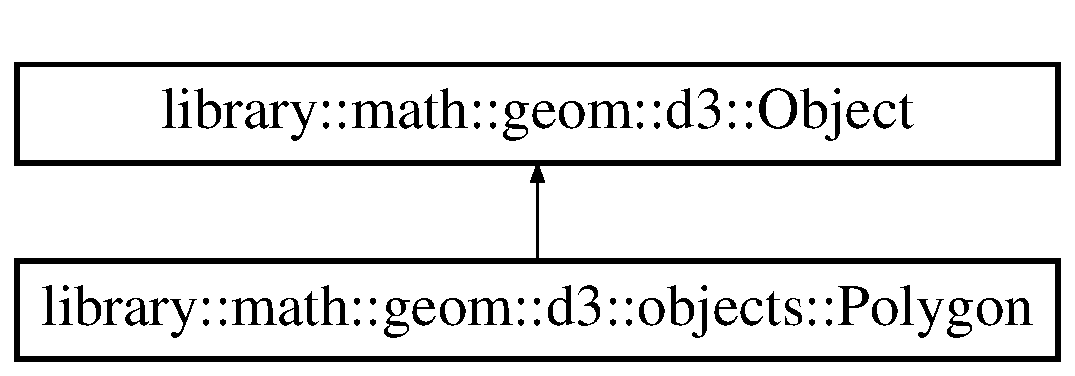
\includegraphics[height=2.000000cm]{classlibrary_1_1math_1_1geom_1_1d3_1_1objects_1_1_polygon}
\end{center}
\end{figure}
\subsection*{Public Types}
\begin{DoxyCompactItemize}
\item 
typedef \hyperlink{classlibrary_1_1math_1_1geom_1_1d3_1_1objects_1_1_point}{Point} \hyperlink{classlibrary_1_1math_1_1geom_1_1d3_1_1objects_1_1_polygon_a12c41d13f2128442c1a15b9eaa08e1d0}{Vertex}
\item 
typedef \hyperlink{classlibrary_1_1math_1_1geom_1_1d3_1_1objects_1_1_segment}{Segment} \hyperlink{classlibrary_1_1math_1_1geom_1_1d3_1_1objects_1_1_polygon_a7962e0559e972fe43eef942ce318fb8d}{Edge}
\item 
typedef \hyperlink{classlibrary_1_1math_1_1geom_1_1d3_1_1objects_1_1_line_string}{Line\+String} \hyperlink{classlibrary_1_1math_1_1geom_1_1d3_1_1objects_1_1_polygon_a3fd1a36a8215242aebb73a2275dc5e45}{Ring}
\end{DoxyCompactItemize}
\subsection*{Public Member Functions}
\begin{DoxyCompactItemize}
\item 
\hyperlink{classlibrary_1_1math_1_1geom_1_1d3_1_1objects_1_1_polygon_aee1e0d3717938cf06752ea06bb623d94}{Polygon} (const \hyperlink{namespacelibrary_1_1math_1_1geom_1_1d3_1_1objects_ae339035ccf9a6f4f0d2945fdcfd76f95}{Polygon2d} \&a\+Polygon, const \hyperlink{classlibrary_1_1math_1_1geom_1_1d3_1_1objects_1_1_point}{Point} \&an\+Origin, const Vector3d \&a\+X\+Axis, const Vector3d \&a\+Y\+Axis)
\begin{DoxyCompactList}\small\item\em Constructor. \end{DoxyCompactList}\item 
virtual \hyperlink{classlibrary_1_1math_1_1geom_1_1d3_1_1objects_1_1_polygon}{Polygon} $\ast$ \hyperlink{classlibrary_1_1math_1_1geom_1_1d3_1_1objects_1_1_polygon_a54440dcce091424ecabdacc30892c2fc}{clone} () const override
\begin{DoxyCompactList}\small\item\em Clone polygon. \end{DoxyCompactList}\item 
bool \hyperlink{classlibrary_1_1math_1_1geom_1_1d3_1_1objects_1_1_polygon_ac8aa92cf9ed3cbcd063df07ce3a89f60}{operator==} (const \hyperlink{classlibrary_1_1math_1_1geom_1_1d3_1_1objects_1_1_polygon}{Polygon} \&a\+Polygon) const
\begin{DoxyCompactList}\small\item\em Equal to operator. \end{DoxyCompactList}\item 
bool \hyperlink{classlibrary_1_1math_1_1geom_1_1d3_1_1objects_1_1_polygon_adaa065fdf80585b0d929151efe07212e}{operator!=} (const \hyperlink{classlibrary_1_1math_1_1geom_1_1d3_1_1objects_1_1_polygon}{Polygon} \&a\+Polygon) const
\begin{DoxyCompactList}\small\item\em Not equal to operator. \end{DoxyCompactList}\item 
virtual bool \hyperlink{classlibrary_1_1math_1_1geom_1_1d3_1_1objects_1_1_polygon_af657beeabcef0af4b8c2fbea4ace6341}{is\+Defined} () const override
\begin{DoxyCompactList}\small\item\em Check if polygon is defined. \end{DoxyCompactList}\item 
bool \hyperlink{classlibrary_1_1math_1_1geom_1_1d3_1_1objects_1_1_polygon_aaf1a30fb520b1165d60017ab83a8f69b}{is\+Near} (const \hyperlink{classlibrary_1_1math_1_1geom_1_1d3_1_1objects_1_1_polygon}{Polygon} \&a\+Polygon, const Real \&a\+Tolerance) const
\begin{DoxyCompactList}\small\item\em Check if polygon is near another polygon. \end{DoxyCompactList}\item 
\hyperlink{namespacelibrary_1_1math_1_1geom_1_1d3_1_1objects_ae339035ccf9a6f4f0d2945fdcfd76f95}{Polygon2d} \hyperlink{classlibrary_1_1math_1_1geom_1_1d3_1_1objects_1_1_polygon_a52a2a342758ed8570aecefa1a18311ec}{get\+Polygon2d} () const
\begin{DoxyCompactList}\small\item\em Get polygon 2D polygon. \end{DoxyCompactList}\item 
\hyperlink{classlibrary_1_1math_1_1geom_1_1d3_1_1objects_1_1_point}{Point} \hyperlink{classlibrary_1_1math_1_1geom_1_1d3_1_1objects_1_1_polygon_add4c768333dd8a58e700b84c67ab1df1}{get\+Origin} () const
\begin{DoxyCompactList}\small\item\em Get polygon origin. \end{DoxyCompactList}\item 
Vector3d \hyperlink{classlibrary_1_1math_1_1geom_1_1d3_1_1objects_1_1_polygon_a1d16c3229601acc55e9ad25510f821e2}{get\+X\+Axis} () const
\begin{DoxyCompactList}\small\item\em Get polygon X axis. \end{DoxyCompactList}\item 
Vector3d \hyperlink{classlibrary_1_1math_1_1geom_1_1d3_1_1objects_1_1_polygon_ac6677598019f6233c1c966b1ddd7914e}{get\+Y\+Axis} () const
\begin{DoxyCompactList}\small\item\em Get polygon Y axis. \end{DoxyCompactList}\item 
Vector3d \hyperlink{classlibrary_1_1math_1_1geom_1_1d3_1_1objects_1_1_polygon_a9df6a1cf7b2d48b9bca560d8794df831}{get\+Normal\+Vector} () const
\begin{DoxyCompactList}\small\item\em Get polygon normal vector. \end{DoxyCompactList}\item 
Size \hyperlink{classlibrary_1_1math_1_1geom_1_1d3_1_1objects_1_1_polygon_aa9ff0300eec7d810c55c2782fcc46cf6}{get\+Edge\+Count} () const
\begin{DoxyCompactList}\small\item\em Get edge count. \end{DoxyCompactList}\item 
Size \hyperlink{classlibrary_1_1math_1_1geom_1_1d3_1_1objects_1_1_polygon_abdd6fd98e2d0aa2ddb69d842cd7e71c1}{get\+Vertex\+Count} () const
\begin{DoxyCompactList}\small\item\em Get vertex count. \end{DoxyCompactList}\item 
\hyperlink{classlibrary_1_1math_1_1geom_1_1d3_1_1objects_1_1_polygon_a7962e0559e972fe43eef942ce318fb8d}{Polygon\+::\+Edge} \hyperlink{classlibrary_1_1math_1_1geom_1_1d3_1_1objects_1_1_polygon_aa595f3aa1b457b453745692ccee8a808}{get\+Edge\+At} (const Index an\+Edge\+Index) const
\begin{DoxyCompactList}\small\item\em Get edge at index. \end{DoxyCompactList}\item 
\hyperlink{classlibrary_1_1math_1_1geom_1_1d3_1_1objects_1_1_polygon_a12c41d13f2128442c1a15b9eaa08e1d0}{Polygon\+::\+Vertex} \hyperlink{classlibrary_1_1math_1_1geom_1_1d3_1_1objects_1_1_polygon_a3a4caaa18b07b7be061ef8b525493c5e}{get\+Vertex\+At} (const Index a\+Vertex\+Index) const
\begin{DoxyCompactList}\small\item\em Get vertex at index. \end{DoxyCompactList}\item 
Array$<$ \hyperlink{classlibrary_1_1math_1_1geom_1_1d3_1_1objects_1_1_polygon_a7962e0559e972fe43eef942ce318fb8d}{Polygon\+::\+Edge} $>$ \hyperlink{classlibrary_1_1math_1_1geom_1_1d3_1_1objects_1_1_polygon_a90b876b752d49e7f7c65976d2f367086}{get\+Edges} () const
\begin{DoxyCompactList}\small\item\em Get polygon edges. \end{DoxyCompactList}\item 
Array$<$ \hyperlink{classlibrary_1_1math_1_1geom_1_1d3_1_1objects_1_1_polygon_a12c41d13f2128442c1a15b9eaa08e1d0}{Polygon\+::\+Vertex} $>$ \hyperlink{classlibrary_1_1math_1_1geom_1_1d3_1_1objects_1_1_polygon_a6df2edc6429946ebd7b9e96524d725fa}{get\+Vertices} () const
\begin{DoxyCompactList}\small\item\em Get polygon vertices. \end{DoxyCompactList}\item 
virtual void \hyperlink{classlibrary_1_1math_1_1geom_1_1d3_1_1objects_1_1_polygon_a6d30846a912386e5e814e0bffa0a4042}{print} (std\+::ostream \&an\+Output\+Stream, bool display\+Decorators=true) const override
\begin{DoxyCompactList}\small\item\em Print polygon. \end{DoxyCompactList}\item 
virtual void \hyperlink{classlibrary_1_1math_1_1geom_1_1d3_1_1objects_1_1_polygon_a712a6f0b739c0f92f3c64873482da217}{apply\+Transformation} (const \hyperlink{classlibrary_1_1math_1_1geom_1_1d3_1_1_transformation}{Transformation} \&a\+Transformation) override
\begin{DoxyCompactList}\small\item\em Apply transformation to polygon. \end{DoxyCompactList}\end{DoxyCompactItemize}
\subsection*{Static Public Member Functions}
\begin{DoxyCompactItemize}
\item 
static \hyperlink{classlibrary_1_1math_1_1geom_1_1d3_1_1objects_1_1_polygon}{Polygon} \hyperlink{classlibrary_1_1math_1_1geom_1_1d3_1_1objects_1_1_polygon_a40a0601975e2ecb41d903fc9b53dd5b8}{Undefined} ()
\begin{DoxyCompactList}\small\item\em Constructs an undefined polygon. \end{DoxyCompactList}\end{DoxyCompactItemize}


\subsection{Detailed Description}
\hyperlink{classlibrary_1_1math_1_1geom_1_1d3_1_1objects_1_1_polygon}{Polygon}. 

A polygon is a plane figure that is bounded by a finite chain of straight line segments closing in a loop to form a closed polygonal chain or circuit. These segments are called its edges, and the points where two edges meet are the polygon\textquotesingle{}s vertices.

https\+://en.wikipedia.\+org/wiki/\+Polygon 

\subsection{Member Typedef Documentation}
\mbox{\Hypertarget{classlibrary_1_1math_1_1geom_1_1d3_1_1objects_1_1_polygon_a7962e0559e972fe43eef942ce318fb8d}\label{classlibrary_1_1math_1_1geom_1_1d3_1_1objects_1_1_polygon_a7962e0559e972fe43eef942ce318fb8d}} 
\index{library\+::math\+::geom\+::d3\+::objects\+::\+Polygon@{library\+::math\+::geom\+::d3\+::objects\+::\+Polygon}!Edge@{Edge}}
\index{Edge@{Edge}!library\+::math\+::geom\+::d3\+::objects\+::\+Polygon@{library\+::math\+::geom\+::d3\+::objects\+::\+Polygon}}
\subsubsection{\texorpdfstring{Edge}{Edge}}
{\footnotesize\ttfamily typedef \hyperlink{classlibrary_1_1math_1_1geom_1_1d3_1_1objects_1_1_segment}{Segment} \hyperlink{classlibrary_1_1math_1_1geom_1_1d3_1_1objects_1_1_polygon_a7962e0559e972fe43eef942ce318fb8d}{library\+::math\+::geom\+::d3\+::objects\+::\+Polygon\+::\+Edge}}

\mbox{\Hypertarget{classlibrary_1_1math_1_1geom_1_1d3_1_1objects_1_1_polygon_a3fd1a36a8215242aebb73a2275dc5e45}\label{classlibrary_1_1math_1_1geom_1_1d3_1_1objects_1_1_polygon_a3fd1a36a8215242aebb73a2275dc5e45}} 
\index{library\+::math\+::geom\+::d3\+::objects\+::\+Polygon@{library\+::math\+::geom\+::d3\+::objects\+::\+Polygon}!Ring@{Ring}}
\index{Ring@{Ring}!library\+::math\+::geom\+::d3\+::objects\+::\+Polygon@{library\+::math\+::geom\+::d3\+::objects\+::\+Polygon}}
\subsubsection{\texorpdfstring{Ring}{Ring}}
{\footnotesize\ttfamily typedef \hyperlink{classlibrary_1_1math_1_1geom_1_1d3_1_1objects_1_1_line_string}{Line\+String} \hyperlink{classlibrary_1_1math_1_1geom_1_1d3_1_1objects_1_1_polygon_a3fd1a36a8215242aebb73a2275dc5e45}{library\+::math\+::geom\+::d3\+::objects\+::\+Polygon\+::\+Ring}}

\mbox{\Hypertarget{classlibrary_1_1math_1_1geom_1_1d3_1_1objects_1_1_polygon_a12c41d13f2128442c1a15b9eaa08e1d0}\label{classlibrary_1_1math_1_1geom_1_1d3_1_1objects_1_1_polygon_a12c41d13f2128442c1a15b9eaa08e1d0}} 
\index{library\+::math\+::geom\+::d3\+::objects\+::\+Polygon@{library\+::math\+::geom\+::d3\+::objects\+::\+Polygon}!Vertex@{Vertex}}
\index{Vertex@{Vertex}!library\+::math\+::geom\+::d3\+::objects\+::\+Polygon@{library\+::math\+::geom\+::d3\+::objects\+::\+Polygon}}
\subsubsection{\texorpdfstring{Vertex}{Vertex}}
{\footnotesize\ttfamily typedef \hyperlink{classlibrary_1_1math_1_1geom_1_1d3_1_1objects_1_1_point}{Point} \hyperlink{classlibrary_1_1math_1_1geom_1_1d3_1_1objects_1_1_polygon_a12c41d13f2128442c1a15b9eaa08e1d0}{library\+::math\+::geom\+::d3\+::objects\+::\+Polygon\+::\+Vertex}}



\subsection{Constructor \& Destructor Documentation}
\mbox{\Hypertarget{classlibrary_1_1math_1_1geom_1_1d3_1_1objects_1_1_polygon_aee1e0d3717938cf06752ea06bb623d94}\label{classlibrary_1_1math_1_1geom_1_1d3_1_1objects_1_1_polygon_aee1e0d3717938cf06752ea06bb623d94}} 
\index{library\+::math\+::geom\+::d3\+::objects\+::\+Polygon@{library\+::math\+::geom\+::d3\+::objects\+::\+Polygon}!Polygon@{Polygon}}
\index{Polygon@{Polygon}!library\+::math\+::geom\+::d3\+::objects\+::\+Polygon@{library\+::math\+::geom\+::d3\+::objects\+::\+Polygon}}
\subsubsection{\texorpdfstring{Polygon()}{Polygon()}}
{\footnotesize\ttfamily library\+::math\+::geom\+::d3\+::objects\+::\+Polygon\+::\+Polygon (\begin{DoxyParamCaption}\item[{const \hyperlink{namespacelibrary_1_1math_1_1geom_1_1d3_1_1objects_ae339035ccf9a6f4f0d2945fdcfd76f95}{Polygon2d} \&}]{a\+Polygon,  }\item[{const \hyperlink{classlibrary_1_1math_1_1geom_1_1d3_1_1objects_1_1_point}{Point} \&}]{an\+Origin,  }\item[{const Vector3d \&}]{a\+X\+Axis,  }\item[{const Vector3d \&}]{a\+Y\+Axis }\end{DoxyParamCaption})}



Constructor. 


\begin{DoxyCode}
\hyperlink{namespacelibrary_1_1math_1_1geom_1_1d3_1_1objects_ae339035ccf9a6f4f0d2945fdcfd76f95}{Polygon2d} polygon2d = \{ \{ \{ 0.0, 0.0 \}, \{ 1.0, 0.0 \}, \{ 1.0, 1.0 \}, \{ 0.0, 1.0 \} \} \} ;
Point origin = \{ 1.0, 2.0, 3.0 \} ;
\hyperlink{namespacelibrary_1_1math_1_1obj_a977e84e9bf317a4e7dd9d6d671d6da2f}{Vector3d} xAxis = \{ 1.0, 0.0, 0.0 \} ;
\hyperlink{namespacelibrary_1_1math_1_1obj_a977e84e9bf317a4e7dd9d6d671d6da2f}{Vector3d} yAxis = \{ 0.0, 1.0, 0.0 \} ;
\hyperlink{classlibrary_1_1math_1_1geom_1_1d3_1_1objects_1_1_polygon_aee1e0d3717938cf06752ea06bb623d94}{Polygon} polygon = \{ polygon2d, origin, xAxis, yAxis \} ;
\end{DoxyCode}



\begin{DoxyParams}[1]{Parameters}
\mbox{\tt in}  & {\em a\+Polygon} & A 2D polygon \\
\hline
\mbox{\tt in}  & {\em an\+Origin} & An origin \\
\hline
\mbox{\tt in}  & {\em a\+X\+Axis} & A X axis \\
\hline
\mbox{\tt in}  & {\em a\+Y\+Axis} & A Y axis \\
\hline
\end{DoxyParams}


\subsection{Member Function Documentation}
\mbox{\Hypertarget{classlibrary_1_1math_1_1geom_1_1d3_1_1objects_1_1_polygon_a712a6f0b739c0f92f3c64873482da217}\label{classlibrary_1_1math_1_1geom_1_1d3_1_1objects_1_1_polygon_a712a6f0b739c0f92f3c64873482da217}} 
\index{library\+::math\+::geom\+::d3\+::objects\+::\+Polygon@{library\+::math\+::geom\+::d3\+::objects\+::\+Polygon}!apply\+Transformation@{apply\+Transformation}}
\index{apply\+Transformation@{apply\+Transformation}!library\+::math\+::geom\+::d3\+::objects\+::\+Polygon@{library\+::math\+::geom\+::d3\+::objects\+::\+Polygon}}
\subsubsection{\texorpdfstring{apply\+Transformation()}{applyTransformation()}}
{\footnotesize\ttfamily void library\+::math\+::geom\+::d3\+::objects\+::\+Polygon\+::apply\+Transformation (\begin{DoxyParamCaption}\item[{const \hyperlink{classlibrary_1_1math_1_1geom_1_1d3_1_1_transformation}{Transformation} \&}]{a\+Transformation }\end{DoxyParamCaption})\hspace{0.3cm}{\ttfamily [override]}, {\ttfamily [virtual]}}



Apply transformation to polygon. 


\begin{DoxyParams}[1]{Parameters}
\mbox{\tt in}  & {\em a\+Transformation} & A transformation \\
\hline
\end{DoxyParams}


Implements \hyperlink{classlibrary_1_1math_1_1geom_1_1d3_1_1_object_a5fc47b1ee5d9a28efc6010d3d1512470}{library\+::math\+::geom\+::d3\+::\+Object}.

\mbox{\Hypertarget{classlibrary_1_1math_1_1geom_1_1d3_1_1objects_1_1_polygon_a54440dcce091424ecabdacc30892c2fc}\label{classlibrary_1_1math_1_1geom_1_1d3_1_1objects_1_1_polygon_a54440dcce091424ecabdacc30892c2fc}} 
\index{library\+::math\+::geom\+::d3\+::objects\+::\+Polygon@{library\+::math\+::geom\+::d3\+::objects\+::\+Polygon}!clone@{clone}}
\index{clone@{clone}!library\+::math\+::geom\+::d3\+::objects\+::\+Polygon@{library\+::math\+::geom\+::d3\+::objects\+::\+Polygon}}
\subsubsection{\texorpdfstring{clone()}{clone()}}
{\footnotesize\ttfamily \hyperlink{classlibrary_1_1math_1_1geom_1_1d3_1_1objects_1_1_polygon}{Polygon} $\ast$ library\+::math\+::geom\+::d3\+::objects\+::\+Polygon\+::clone (\begin{DoxyParamCaption}{ }\end{DoxyParamCaption}) const\hspace{0.3cm}{\ttfamily [override]}, {\ttfamily [virtual]}}



Clone polygon. 

\begin{DoxyReturn}{Returns}
Pointer to cloned polygon 
\end{DoxyReturn}


Implements \hyperlink{classlibrary_1_1math_1_1geom_1_1d3_1_1_object_a1a784c6b359e0eb97cd34fabc42f2f3f}{library\+::math\+::geom\+::d3\+::\+Object}.

\mbox{\Hypertarget{classlibrary_1_1math_1_1geom_1_1d3_1_1objects_1_1_polygon_aa595f3aa1b457b453745692ccee8a808}\label{classlibrary_1_1math_1_1geom_1_1d3_1_1objects_1_1_polygon_aa595f3aa1b457b453745692ccee8a808}} 
\index{library\+::math\+::geom\+::d3\+::objects\+::\+Polygon@{library\+::math\+::geom\+::d3\+::objects\+::\+Polygon}!get\+Edge\+At@{get\+Edge\+At}}
\index{get\+Edge\+At@{get\+Edge\+At}!library\+::math\+::geom\+::d3\+::objects\+::\+Polygon@{library\+::math\+::geom\+::d3\+::objects\+::\+Polygon}}
\subsubsection{\texorpdfstring{get\+Edge\+At()}{getEdgeAt()}}
{\footnotesize\ttfamily \hyperlink{classlibrary_1_1math_1_1geom_1_1d3_1_1objects_1_1_polygon_a7962e0559e972fe43eef942ce318fb8d}{Polygon\+::\+Edge} library\+::math\+::geom\+::d3\+::objects\+::\+Polygon\+::get\+Edge\+At (\begin{DoxyParamCaption}\item[{const Index}]{an\+Edge\+Index }\end{DoxyParamCaption}) const}



Get edge at index. 


\begin{DoxyParams}[1]{Parameters}
\mbox{\tt in}  & {\em an\+Edge\+Index} & An edge index \\
\hline
\end{DoxyParams}
\begin{DoxyReturn}{Returns}
Edge (segment) 
\end{DoxyReturn}
\mbox{\Hypertarget{classlibrary_1_1math_1_1geom_1_1d3_1_1objects_1_1_polygon_aa9ff0300eec7d810c55c2782fcc46cf6}\label{classlibrary_1_1math_1_1geom_1_1d3_1_1objects_1_1_polygon_aa9ff0300eec7d810c55c2782fcc46cf6}} 
\index{library\+::math\+::geom\+::d3\+::objects\+::\+Polygon@{library\+::math\+::geom\+::d3\+::objects\+::\+Polygon}!get\+Edge\+Count@{get\+Edge\+Count}}
\index{get\+Edge\+Count@{get\+Edge\+Count}!library\+::math\+::geom\+::d3\+::objects\+::\+Polygon@{library\+::math\+::geom\+::d3\+::objects\+::\+Polygon}}
\subsubsection{\texorpdfstring{get\+Edge\+Count()}{getEdgeCount()}}
{\footnotesize\ttfamily Size library\+::math\+::geom\+::d3\+::objects\+::\+Polygon\+::get\+Edge\+Count (\begin{DoxyParamCaption}{ }\end{DoxyParamCaption}) const}



Get edge count. 

\begin{DoxyReturn}{Returns}
Edge count 
\end{DoxyReturn}
\mbox{\Hypertarget{classlibrary_1_1math_1_1geom_1_1d3_1_1objects_1_1_polygon_a90b876b752d49e7f7c65976d2f367086}\label{classlibrary_1_1math_1_1geom_1_1d3_1_1objects_1_1_polygon_a90b876b752d49e7f7c65976d2f367086}} 
\index{library\+::math\+::geom\+::d3\+::objects\+::\+Polygon@{library\+::math\+::geom\+::d3\+::objects\+::\+Polygon}!get\+Edges@{get\+Edges}}
\index{get\+Edges@{get\+Edges}!library\+::math\+::geom\+::d3\+::objects\+::\+Polygon@{library\+::math\+::geom\+::d3\+::objects\+::\+Polygon}}
\subsubsection{\texorpdfstring{get\+Edges()}{getEdges()}}
{\footnotesize\ttfamily Array$<$ \hyperlink{classlibrary_1_1math_1_1geom_1_1d3_1_1objects_1_1_polygon_a7962e0559e972fe43eef942ce318fb8d}{Polygon\+::\+Edge} $>$ library\+::math\+::geom\+::d3\+::objects\+::\+Polygon\+::get\+Edges (\begin{DoxyParamCaption}{ }\end{DoxyParamCaption}) const}



Get polygon edges. 

\begin{DoxyReturn}{Returns}
\hyperlink{classlibrary_1_1math_1_1geom_1_1d3_1_1objects_1_1_polygon}{Polygon} edges 
\end{DoxyReturn}
\mbox{\Hypertarget{classlibrary_1_1math_1_1geom_1_1d3_1_1objects_1_1_polygon_a9df6a1cf7b2d48b9bca560d8794df831}\label{classlibrary_1_1math_1_1geom_1_1d3_1_1objects_1_1_polygon_a9df6a1cf7b2d48b9bca560d8794df831}} 
\index{library\+::math\+::geom\+::d3\+::objects\+::\+Polygon@{library\+::math\+::geom\+::d3\+::objects\+::\+Polygon}!get\+Normal\+Vector@{get\+Normal\+Vector}}
\index{get\+Normal\+Vector@{get\+Normal\+Vector}!library\+::math\+::geom\+::d3\+::objects\+::\+Polygon@{library\+::math\+::geom\+::d3\+::objects\+::\+Polygon}}
\subsubsection{\texorpdfstring{get\+Normal\+Vector()}{getNormalVector()}}
{\footnotesize\ttfamily Vector3d library\+::math\+::geom\+::d3\+::objects\+::\+Polygon\+::get\+Normal\+Vector (\begin{DoxyParamCaption}{ }\end{DoxyParamCaption}) const}



Get polygon normal vector. 

\begin{DoxyReturn}{Returns}
\hyperlink{classlibrary_1_1math_1_1geom_1_1d3_1_1objects_1_1_polygon}{Polygon} normal vector 
\end{DoxyReturn}
\mbox{\Hypertarget{classlibrary_1_1math_1_1geom_1_1d3_1_1objects_1_1_polygon_add4c768333dd8a58e700b84c67ab1df1}\label{classlibrary_1_1math_1_1geom_1_1d3_1_1objects_1_1_polygon_add4c768333dd8a58e700b84c67ab1df1}} 
\index{library\+::math\+::geom\+::d3\+::objects\+::\+Polygon@{library\+::math\+::geom\+::d3\+::objects\+::\+Polygon}!get\+Origin@{get\+Origin}}
\index{get\+Origin@{get\+Origin}!library\+::math\+::geom\+::d3\+::objects\+::\+Polygon@{library\+::math\+::geom\+::d3\+::objects\+::\+Polygon}}
\subsubsection{\texorpdfstring{get\+Origin()}{getOrigin()}}
{\footnotesize\ttfamily \hyperlink{classlibrary_1_1math_1_1geom_1_1d3_1_1objects_1_1_point}{Point} library\+::math\+::geom\+::d3\+::objects\+::\+Polygon\+::get\+Origin (\begin{DoxyParamCaption}{ }\end{DoxyParamCaption}) const}



Get polygon origin. 

\begin{DoxyReturn}{Returns}
\hyperlink{classlibrary_1_1math_1_1geom_1_1d3_1_1objects_1_1_polygon}{Polygon} origin 
\end{DoxyReturn}
\mbox{\Hypertarget{classlibrary_1_1math_1_1geom_1_1d3_1_1objects_1_1_polygon_a52a2a342758ed8570aecefa1a18311ec}\label{classlibrary_1_1math_1_1geom_1_1d3_1_1objects_1_1_polygon_a52a2a342758ed8570aecefa1a18311ec}} 
\index{library\+::math\+::geom\+::d3\+::objects\+::\+Polygon@{library\+::math\+::geom\+::d3\+::objects\+::\+Polygon}!get\+Polygon2d@{get\+Polygon2d}}
\index{get\+Polygon2d@{get\+Polygon2d}!library\+::math\+::geom\+::d3\+::objects\+::\+Polygon@{library\+::math\+::geom\+::d3\+::objects\+::\+Polygon}}
\subsubsection{\texorpdfstring{get\+Polygon2d()}{getPolygon2d()}}
{\footnotesize\ttfamily \hyperlink{namespacelibrary_1_1math_1_1geom_1_1d3_1_1objects_ae339035ccf9a6f4f0d2945fdcfd76f95}{Polygon2d} library\+::math\+::geom\+::d3\+::objects\+::\+Polygon\+::get\+Polygon2d (\begin{DoxyParamCaption}{ }\end{DoxyParamCaption}) const}



Get polygon 2D polygon. 

\begin{DoxyReturn}{Returns}
\hyperlink{classlibrary_1_1math_1_1geom_1_1d3_1_1objects_1_1_polygon}{Polygon} 2D polygon 
\end{DoxyReturn}
\mbox{\Hypertarget{classlibrary_1_1math_1_1geom_1_1d3_1_1objects_1_1_polygon_a3a4caaa18b07b7be061ef8b525493c5e}\label{classlibrary_1_1math_1_1geom_1_1d3_1_1objects_1_1_polygon_a3a4caaa18b07b7be061ef8b525493c5e}} 
\index{library\+::math\+::geom\+::d3\+::objects\+::\+Polygon@{library\+::math\+::geom\+::d3\+::objects\+::\+Polygon}!get\+Vertex\+At@{get\+Vertex\+At}}
\index{get\+Vertex\+At@{get\+Vertex\+At}!library\+::math\+::geom\+::d3\+::objects\+::\+Polygon@{library\+::math\+::geom\+::d3\+::objects\+::\+Polygon}}
\subsubsection{\texorpdfstring{get\+Vertex\+At()}{getVertexAt()}}
{\footnotesize\ttfamily \hyperlink{classlibrary_1_1math_1_1geom_1_1d3_1_1objects_1_1_polygon_a12c41d13f2128442c1a15b9eaa08e1d0}{Polygon\+::\+Vertex} library\+::math\+::geom\+::d3\+::objects\+::\+Polygon\+::get\+Vertex\+At (\begin{DoxyParamCaption}\item[{const Index}]{a\+Vertex\+Index }\end{DoxyParamCaption}) const}



Get vertex at index. 


\begin{DoxyParams}[1]{Parameters}
\mbox{\tt in}  & {\em a\+Vertex\+Index} & A vertex index \\
\hline
\end{DoxyParams}
\begin{DoxyReturn}{Returns}
Vertex 
\end{DoxyReturn}
\mbox{\Hypertarget{classlibrary_1_1math_1_1geom_1_1d3_1_1objects_1_1_polygon_abdd6fd98e2d0aa2ddb69d842cd7e71c1}\label{classlibrary_1_1math_1_1geom_1_1d3_1_1objects_1_1_polygon_abdd6fd98e2d0aa2ddb69d842cd7e71c1}} 
\index{library\+::math\+::geom\+::d3\+::objects\+::\+Polygon@{library\+::math\+::geom\+::d3\+::objects\+::\+Polygon}!get\+Vertex\+Count@{get\+Vertex\+Count}}
\index{get\+Vertex\+Count@{get\+Vertex\+Count}!library\+::math\+::geom\+::d3\+::objects\+::\+Polygon@{library\+::math\+::geom\+::d3\+::objects\+::\+Polygon}}
\subsubsection{\texorpdfstring{get\+Vertex\+Count()}{getVertexCount()}}
{\footnotesize\ttfamily Size library\+::math\+::geom\+::d3\+::objects\+::\+Polygon\+::get\+Vertex\+Count (\begin{DoxyParamCaption}{ }\end{DoxyParamCaption}) const}



Get vertex count. 

\begin{DoxyReturn}{Returns}
Vertex count 
\end{DoxyReturn}
\mbox{\Hypertarget{classlibrary_1_1math_1_1geom_1_1d3_1_1objects_1_1_polygon_a6df2edc6429946ebd7b9e96524d725fa}\label{classlibrary_1_1math_1_1geom_1_1d3_1_1objects_1_1_polygon_a6df2edc6429946ebd7b9e96524d725fa}} 
\index{library\+::math\+::geom\+::d3\+::objects\+::\+Polygon@{library\+::math\+::geom\+::d3\+::objects\+::\+Polygon}!get\+Vertices@{get\+Vertices}}
\index{get\+Vertices@{get\+Vertices}!library\+::math\+::geom\+::d3\+::objects\+::\+Polygon@{library\+::math\+::geom\+::d3\+::objects\+::\+Polygon}}
\subsubsection{\texorpdfstring{get\+Vertices()}{getVertices()}}
{\footnotesize\ttfamily Array$<$ \hyperlink{classlibrary_1_1math_1_1geom_1_1d3_1_1objects_1_1_polygon_a12c41d13f2128442c1a15b9eaa08e1d0}{Polygon\+::\+Vertex} $>$ library\+::math\+::geom\+::d3\+::objects\+::\+Polygon\+::get\+Vertices (\begin{DoxyParamCaption}{ }\end{DoxyParamCaption}) const}



Get polygon vertices. 

\begin{DoxyReturn}{Returns}
\hyperlink{classlibrary_1_1math_1_1geom_1_1d3_1_1objects_1_1_polygon}{Polygon} vertices 
\end{DoxyReturn}
\mbox{\Hypertarget{classlibrary_1_1math_1_1geom_1_1d3_1_1objects_1_1_polygon_a1d16c3229601acc55e9ad25510f821e2}\label{classlibrary_1_1math_1_1geom_1_1d3_1_1objects_1_1_polygon_a1d16c3229601acc55e9ad25510f821e2}} 
\index{library\+::math\+::geom\+::d3\+::objects\+::\+Polygon@{library\+::math\+::geom\+::d3\+::objects\+::\+Polygon}!get\+X\+Axis@{get\+X\+Axis}}
\index{get\+X\+Axis@{get\+X\+Axis}!library\+::math\+::geom\+::d3\+::objects\+::\+Polygon@{library\+::math\+::geom\+::d3\+::objects\+::\+Polygon}}
\subsubsection{\texorpdfstring{get\+X\+Axis()}{getXAxis()}}
{\footnotesize\ttfamily Vector3d library\+::math\+::geom\+::d3\+::objects\+::\+Polygon\+::get\+X\+Axis (\begin{DoxyParamCaption}{ }\end{DoxyParamCaption}) const}



Get polygon X axis. 

\begin{DoxyReturn}{Returns}
\hyperlink{classlibrary_1_1math_1_1geom_1_1d3_1_1objects_1_1_polygon}{Polygon} X axis 
\end{DoxyReturn}
\mbox{\Hypertarget{classlibrary_1_1math_1_1geom_1_1d3_1_1objects_1_1_polygon_ac6677598019f6233c1c966b1ddd7914e}\label{classlibrary_1_1math_1_1geom_1_1d3_1_1objects_1_1_polygon_ac6677598019f6233c1c966b1ddd7914e}} 
\index{library\+::math\+::geom\+::d3\+::objects\+::\+Polygon@{library\+::math\+::geom\+::d3\+::objects\+::\+Polygon}!get\+Y\+Axis@{get\+Y\+Axis}}
\index{get\+Y\+Axis@{get\+Y\+Axis}!library\+::math\+::geom\+::d3\+::objects\+::\+Polygon@{library\+::math\+::geom\+::d3\+::objects\+::\+Polygon}}
\subsubsection{\texorpdfstring{get\+Y\+Axis()}{getYAxis()}}
{\footnotesize\ttfamily Vector3d library\+::math\+::geom\+::d3\+::objects\+::\+Polygon\+::get\+Y\+Axis (\begin{DoxyParamCaption}{ }\end{DoxyParamCaption}) const}



Get polygon Y axis. 

\begin{DoxyReturn}{Returns}
\hyperlink{classlibrary_1_1math_1_1geom_1_1d3_1_1objects_1_1_polygon}{Polygon} Y axis 
\end{DoxyReturn}
\mbox{\Hypertarget{classlibrary_1_1math_1_1geom_1_1d3_1_1objects_1_1_polygon_af657beeabcef0af4b8c2fbea4ace6341}\label{classlibrary_1_1math_1_1geom_1_1d3_1_1objects_1_1_polygon_af657beeabcef0af4b8c2fbea4ace6341}} 
\index{library\+::math\+::geom\+::d3\+::objects\+::\+Polygon@{library\+::math\+::geom\+::d3\+::objects\+::\+Polygon}!is\+Defined@{is\+Defined}}
\index{is\+Defined@{is\+Defined}!library\+::math\+::geom\+::d3\+::objects\+::\+Polygon@{library\+::math\+::geom\+::d3\+::objects\+::\+Polygon}}
\subsubsection{\texorpdfstring{is\+Defined()}{isDefined()}}
{\footnotesize\ttfamily bool library\+::math\+::geom\+::d3\+::objects\+::\+Polygon\+::is\+Defined (\begin{DoxyParamCaption}{ }\end{DoxyParamCaption}) const\hspace{0.3cm}{\ttfamily [override]}, {\ttfamily [virtual]}}



Check if polygon is defined. 

\begin{DoxyReturn}{Returns}
True if polygon is defined 
\end{DoxyReturn}


Implements \hyperlink{classlibrary_1_1math_1_1geom_1_1d3_1_1_object_a2216442e322f0c3ca5f01a4efa22baf7}{library\+::math\+::geom\+::d3\+::\+Object}.

\mbox{\Hypertarget{classlibrary_1_1math_1_1geom_1_1d3_1_1objects_1_1_polygon_aaf1a30fb520b1165d60017ab83a8f69b}\label{classlibrary_1_1math_1_1geom_1_1d3_1_1objects_1_1_polygon_aaf1a30fb520b1165d60017ab83a8f69b}} 
\index{library\+::math\+::geom\+::d3\+::objects\+::\+Polygon@{library\+::math\+::geom\+::d3\+::objects\+::\+Polygon}!is\+Near@{is\+Near}}
\index{is\+Near@{is\+Near}!library\+::math\+::geom\+::d3\+::objects\+::\+Polygon@{library\+::math\+::geom\+::d3\+::objects\+::\+Polygon}}
\subsubsection{\texorpdfstring{is\+Near()}{isNear()}}
{\footnotesize\ttfamily bool library\+::math\+::geom\+::d3\+::objects\+::\+Polygon\+::is\+Near (\begin{DoxyParamCaption}\item[{const \hyperlink{classlibrary_1_1math_1_1geom_1_1d3_1_1objects_1_1_polygon}{Polygon} \&}]{a\+Polygon,  }\item[{const Real \&}]{a\+Tolerance }\end{DoxyParamCaption}) const}



Check if polygon is near another polygon. 


\begin{DoxyParams}[1]{Parameters}
\mbox{\tt in}  & {\em a\+Polygon} & A polygon \\
\hline
\mbox{\tt in}  & {\em a\+Tolerance} & A tolerance \\
\hline
\end{DoxyParams}
\begin{DoxyReturn}{Returns}
True if polygon is near another polygon 
\end{DoxyReturn}
\mbox{\Hypertarget{classlibrary_1_1math_1_1geom_1_1d3_1_1objects_1_1_polygon_adaa065fdf80585b0d929151efe07212e}\label{classlibrary_1_1math_1_1geom_1_1d3_1_1objects_1_1_polygon_adaa065fdf80585b0d929151efe07212e}} 
\index{library\+::math\+::geom\+::d3\+::objects\+::\+Polygon@{library\+::math\+::geom\+::d3\+::objects\+::\+Polygon}!operator"!=@{operator"!=}}
\index{operator"!=@{operator"!=}!library\+::math\+::geom\+::d3\+::objects\+::\+Polygon@{library\+::math\+::geom\+::d3\+::objects\+::\+Polygon}}
\subsubsection{\texorpdfstring{operator"!=()}{operator!=()}}
{\footnotesize\ttfamily bool library\+::math\+::geom\+::d3\+::objects\+::\+Polygon\+::operator!= (\begin{DoxyParamCaption}\item[{const \hyperlink{classlibrary_1_1math_1_1geom_1_1d3_1_1objects_1_1_polygon}{Polygon} \&}]{a\+Polygon }\end{DoxyParamCaption}) const}



Not equal to operator. 


\begin{DoxyParams}[1]{Parameters}
\mbox{\tt in}  & {\em a\+Polygon} & A polygon \\
\hline
\end{DoxyParams}
\begin{DoxyReturn}{Returns}
True if polygons not are equal 
\end{DoxyReturn}
\mbox{\Hypertarget{classlibrary_1_1math_1_1geom_1_1d3_1_1objects_1_1_polygon_ac8aa92cf9ed3cbcd063df07ce3a89f60}\label{classlibrary_1_1math_1_1geom_1_1d3_1_1objects_1_1_polygon_ac8aa92cf9ed3cbcd063df07ce3a89f60}} 
\index{library\+::math\+::geom\+::d3\+::objects\+::\+Polygon@{library\+::math\+::geom\+::d3\+::objects\+::\+Polygon}!operator==@{operator==}}
\index{operator==@{operator==}!library\+::math\+::geom\+::d3\+::objects\+::\+Polygon@{library\+::math\+::geom\+::d3\+::objects\+::\+Polygon}}
\subsubsection{\texorpdfstring{operator==()}{operator==()}}
{\footnotesize\ttfamily bool library\+::math\+::geom\+::d3\+::objects\+::\+Polygon\+::operator== (\begin{DoxyParamCaption}\item[{const \hyperlink{classlibrary_1_1math_1_1geom_1_1d3_1_1objects_1_1_polygon}{Polygon} \&}]{a\+Polygon }\end{DoxyParamCaption}) const}



Equal to operator. 


\begin{DoxyParams}[1]{Parameters}
\mbox{\tt in}  & {\em a\+Polygon} & A polygon \\
\hline
\end{DoxyParams}
\begin{DoxyReturn}{Returns}
True if polygons are equal 
\end{DoxyReturn}
\mbox{\Hypertarget{classlibrary_1_1math_1_1geom_1_1d3_1_1objects_1_1_polygon_a6d30846a912386e5e814e0bffa0a4042}\label{classlibrary_1_1math_1_1geom_1_1d3_1_1objects_1_1_polygon_a6d30846a912386e5e814e0bffa0a4042}} 
\index{library\+::math\+::geom\+::d3\+::objects\+::\+Polygon@{library\+::math\+::geom\+::d3\+::objects\+::\+Polygon}!print@{print}}
\index{print@{print}!library\+::math\+::geom\+::d3\+::objects\+::\+Polygon@{library\+::math\+::geom\+::d3\+::objects\+::\+Polygon}}
\subsubsection{\texorpdfstring{print()}{print()}}
{\footnotesize\ttfamily void library\+::math\+::geom\+::d3\+::objects\+::\+Polygon\+::print (\begin{DoxyParamCaption}\item[{std\+::ostream \&}]{an\+Output\+Stream,  }\item[{bool}]{display\+Decorators = {\ttfamily true} }\end{DoxyParamCaption}) const\hspace{0.3cm}{\ttfamily [override]}, {\ttfamily [virtual]}}



Print polygon. 


\begin{DoxyParams}[1]{Parameters}
\mbox{\tt in}  & {\em an\+Output\+Stream} & An output stream \\
\hline
\mbox{\tt in}  & {\em (optional)} & display\+Decorators If true, display decorators \\
\hline
\end{DoxyParams}


Implements \hyperlink{classlibrary_1_1math_1_1geom_1_1d3_1_1_object_aa166f4ce4d116a248f0fc861c75012ca}{library\+::math\+::geom\+::d3\+::\+Object}.

\mbox{\Hypertarget{classlibrary_1_1math_1_1geom_1_1d3_1_1objects_1_1_polygon_a40a0601975e2ecb41d903fc9b53dd5b8}\label{classlibrary_1_1math_1_1geom_1_1d3_1_1objects_1_1_polygon_a40a0601975e2ecb41d903fc9b53dd5b8}} 
\index{library\+::math\+::geom\+::d3\+::objects\+::\+Polygon@{library\+::math\+::geom\+::d3\+::objects\+::\+Polygon}!Undefined@{Undefined}}
\index{Undefined@{Undefined}!library\+::math\+::geom\+::d3\+::objects\+::\+Polygon@{library\+::math\+::geom\+::d3\+::objects\+::\+Polygon}}
\subsubsection{\texorpdfstring{Undefined()}{Undefined()}}
{\footnotesize\ttfamily \hyperlink{classlibrary_1_1math_1_1geom_1_1d3_1_1objects_1_1_polygon}{Polygon} library\+::math\+::geom\+::d3\+::objects\+::\+Polygon\+::\+Undefined (\begin{DoxyParamCaption}{ }\end{DoxyParamCaption})\hspace{0.3cm}{\ttfamily [static]}}



Constructs an undefined polygon. 

\begin{DoxyReturn}{Returns}
Undefined polygon 
\end{DoxyReturn}


The documentation for this class was generated from the following files\+:\begin{DoxyCompactItemize}
\item 
include/\+Library/\+Mathematics/\+Geometry/3\+D/\+Objects/\hyperlink{3_d_2_objects_2_polygon_8hpp}{Polygon.\+hpp}\item 
src/\+Library/\+Mathematics/\+Geometry/3\+D/\+Objects/\hyperlink{3_d_2_objects_2_polygon_8cpp}{Polygon.\+cpp}\end{DoxyCompactItemize}

\hypertarget{classlibrary_1_1math_1_1geom_1_1d3_1_1objects_1_1_pyramid}{}\section{library\+:\+:math\+:\+:geom\+:\+:d3\+:\+:objects\+:\+:Pyramid Class Reference}
\label{classlibrary_1_1math_1_1geom_1_1d3_1_1objects_1_1_pyramid}\index{library\+::math\+::geom\+::d3\+::objects\+::\+Pyramid@{library\+::math\+::geom\+::d3\+::objects\+::\+Pyramid}}


\hyperlink{classlibrary_1_1math_1_1geom_1_1d3_1_1objects_1_1_pyramid}{Pyramid}.  




{\ttfamily \#include $<$Pyramid.\+hpp$>$}

Inheritance diagram for library\+:\+:math\+:\+:geom\+:\+:d3\+:\+:objects\+:\+:Pyramid\+:\begin{figure}[H]
\begin{center}
\leavevmode
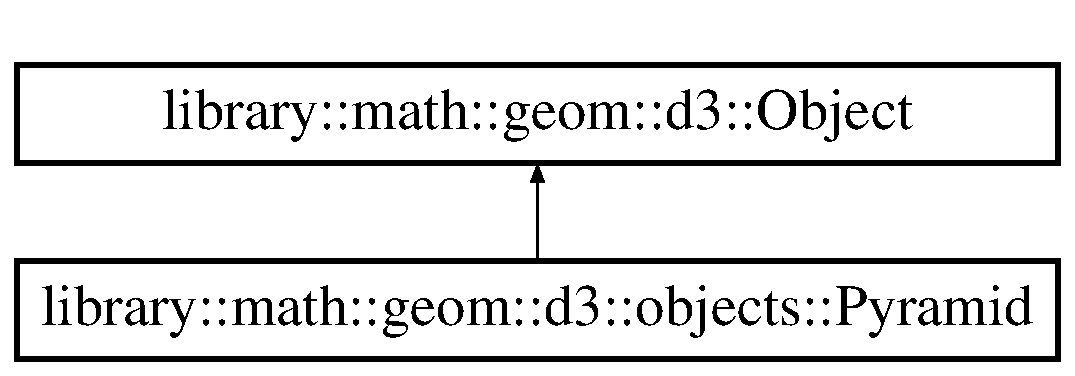
\includegraphics[height=2.000000cm]{classlibrary_1_1math_1_1geom_1_1d3_1_1objects_1_1_pyramid}
\end{center}
\end{figure}
\subsection*{Public Member Functions}
\begin{DoxyCompactItemize}
\item 
\hyperlink{classlibrary_1_1math_1_1geom_1_1d3_1_1objects_1_1_pyramid_aafaaeed187584040b306b7de7ee57fd4}{Pyramid} (const \hyperlink{classlibrary_1_1math_1_1geom_1_1d3_1_1objects_1_1_polygon}{Polygon} \&a\+Base, const \hyperlink{classlibrary_1_1math_1_1geom_1_1d3_1_1objects_1_1_point}{Point} \&an\+Apex)
\begin{DoxyCompactList}\small\item\em Constructor. \end{DoxyCompactList}\item 
virtual \hyperlink{classlibrary_1_1math_1_1geom_1_1d3_1_1objects_1_1_pyramid}{Pyramid} $\ast$ \hyperlink{classlibrary_1_1math_1_1geom_1_1d3_1_1objects_1_1_pyramid_a734bc02bbfec62647743649bf5d2b706}{clone} () const override
\begin{DoxyCompactList}\small\item\em Clone pyramid. \end{DoxyCompactList}\item 
bool \hyperlink{classlibrary_1_1math_1_1geom_1_1d3_1_1objects_1_1_pyramid_adfb99bef5bd74a3b0fe75dcf0c61bd61}{operator==} (const \hyperlink{classlibrary_1_1math_1_1geom_1_1d3_1_1objects_1_1_pyramid}{Pyramid} \&a\+Pyramid) const
\begin{DoxyCompactList}\small\item\em Equal to operator. \end{DoxyCompactList}\item 
bool \hyperlink{classlibrary_1_1math_1_1geom_1_1d3_1_1objects_1_1_pyramid_a2067ce77436b89472125b37446bb6e3d}{operator!=} (const \hyperlink{classlibrary_1_1math_1_1geom_1_1d3_1_1objects_1_1_pyramid}{Pyramid} \&a\+Pyramid) const
\begin{DoxyCompactList}\small\item\em Not equal to operator. \end{DoxyCompactList}\item 
virtual bool \hyperlink{classlibrary_1_1math_1_1geom_1_1d3_1_1objects_1_1_pyramid_a84d92fa1416c288abb5e2616410aa40c}{is\+Defined} () const override
\begin{DoxyCompactList}\small\item\em Check if pyramid is defined. \end{DoxyCompactList}\item 
bool \hyperlink{classlibrary_1_1math_1_1geom_1_1d3_1_1objects_1_1_pyramid_a704dca8e456461a59fe606bd5df06d20}{intersects} (const \hyperlink{classlibrary_1_1math_1_1geom_1_1d3_1_1objects_1_1_sphere}{Sphere} \&a\+Sphere, const Size a\+Discretization\+Level=40) const
\begin{DoxyCompactList}\small\item\em Check if pyramid intersects sphere. \end{DoxyCompactList}\item 
bool \hyperlink{classlibrary_1_1math_1_1geom_1_1d3_1_1objects_1_1_pyramid_a7a79fd414bea507272e6c88ed66eeba8}{intersects} (const \hyperlink{classlibrary_1_1math_1_1geom_1_1d3_1_1objects_1_1_ellipsoid}{Ellipsoid} \&an\+Ellipsoid, const Size a\+Discretization\+Level=40) const
\begin{DoxyCompactList}\small\item\em Check if pyramid intersects ellipsoid. \end{DoxyCompactList}\item 
bool \hyperlink{classlibrary_1_1math_1_1geom_1_1d3_1_1objects_1_1_pyramid_a6f92215d38dcab3319b7585be8019c1d}{contains} (const \hyperlink{classlibrary_1_1math_1_1geom_1_1d3_1_1objects_1_1_point}{Point} \&a\+Point) const
\begin{DoxyCompactList}\small\item\em Check if pyramid contains point. \end{DoxyCompactList}\item 
bool \hyperlink{classlibrary_1_1math_1_1geom_1_1d3_1_1objects_1_1_pyramid_a32e8fd53701cd4d2c0c6b377ca7902c9}{contains} (const \hyperlink{classlibrary_1_1math_1_1geom_1_1d3_1_1objects_1_1_ellipsoid}{Ellipsoid} \&an\+Ellipsoid) const
\begin{DoxyCompactList}\small\item\em Check if pyramid contains ellipsoid. \end{DoxyCompactList}\item 
\hyperlink{classlibrary_1_1math_1_1geom_1_1d3_1_1objects_1_1_polygon}{Polygon} \hyperlink{classlibrary_1_1math_1_1geom_1_1d3_1_1objects_1_1_pyramid_a247e3c188d7919b2043e59d46b67c2ef}{get\+Base} () const
\begin{DoxyCompactList}\small\item\em Get pyramid base. \end{DoxyCompactList}\item 
\hyperlink{classlibrary_1_1math_1_1geom_1_1d3_1_1objects_1_1_point}{Point} \hyperlink{classlibrary_1_1math_1_1geom_1_1d3_1_1objects_1_1_pyramid_af24d52592c3154d633f694411d11396c}{get\+Apex} () const
\begin{DoxyCompactList}\small\item\em Get pyramid apex. \end{DoxyCompactList}\item 
Size \hyperlink{classlibrary_1_1math_1_1geom_1_1d3_1_1objects_1_1_pyramid_ac208d0799c3180c01db9d5d988d73118}{get\+Lateral\+Face\+Count} () const
\begin{DoxyCompactList}\small\item\em Get number of lateral faces. \end{DoxyCompactList}\item 
\hyperlink{classlibrary_1_1math_1_1geom_1_1d3_1_1objects_1_1_polygon}{Polygon} \hyperlink{classlibrary_1_1math_1_1geom_1_1d3_1_1objects_1_1_pyramid_a36f5527c9708f2d44fdddaf7c9ac5ea0}{get\+Lateral\+Face\+At} (const Index a\+Lateral\+Face\+Index) const
\begin{DoxyCompactList}\small\item\em Get lateral face at index. \end{DoxyCompactList}\item 
Array$<$ \hyperlink{classlibrary_1_1math_1_1geom_1_1d3_1_1objects_1_1_ray}{Ray} $>$ \hyperlink{classlibrary_1_1math_1_1geom_1_1d3_1_1objects_1_1_pyramid_a455aad7bd45e9a180cc8eb0082f9bfcf}{get\+Rays\+Of\+Lateral\+Face\+At} (const Index a\+Lateral\+Face\+Index, const Size a\+Ray\+Count=2) const
\begin{DoxyCompactList}\small\item\em Get rays of lateral face at index. \end{DoxyCompactList}\item 
Array$<$ \hyperlink{classlibrary_1_1math_1_1geom_1_1d3_1_1objects_1_1_ray}{Ray} $>$ \hyperlink{classlibrary_1_1math_1_1geom_1_1d3_1_1objects_1_1_pyramid_ab73146c08e94315b9a7dc2392e450f79}{get\+Rays\+Of\+Lateral\+Faces} (const Size a\+Ray\+Count=0) const
\begin{DoxyCompactList}\small\item\em Get rays of lateral faces. \end{DoxyCompactList}\item 
\hyperlink{classlibrary_1_1math_1_1geom_1_1d3_1_1_intersection}{Intersection} \hyperlink{classlibrary_1_1math_1_1geom_1_1d3_1_1objects_1_1_pyramid_a4f3d9b5270a86b462c33c0b1ddeee873}{intersection\+With} (const \hyperlink{classlibrary_1_1math_1_1geom_1_1d3_1_1objects_1_1_sphere}{Sphere} \&a\+Sphere, const bool only\+In\+Sight=false, const Size a\+Discretization\+Level=40) const
\begin{DoxyCompactList}\small\item\em Compute intersection of pyramid with sphere. \end{DoxyCompactList}\item 
\hyperlink{classlibrary_1_1math_1_1geom_1_1d3_1_1_intersection}{Intersection} \hyperlink{classlibrary_1_1math_1_1geom_1_1d3_1_1objects_1_1_pyramid_a299c41f4cbd61ec24799815dfd7c386d}{intersection\+With} (const \hyperlink{classlibrary_1_1math_1_1geom_1_1d3_1_1objects_1_1_ellipsoid}{Ellipsoid} \&an\+Ellipsoid, const bool only\+In\+Sight=false, const Size a\+Discretization\+Level=40) const
\begin{DoxyCompactList}\small\item\em Compute intersection of pyramid with ellipsoid. \end{DoxyCompactList}\item 
virtual void \hyperlink{classlibrary_1_1math_1_1geom_1_1d3_1_1objects_1_1_pyramid_a150cd331b3dc6e36c74b37bc6988f019}{print} (std\+::ostream \&an\+Output\+Stream, bool display\+Decorators=true) const override
\begin{DoxyCompactList}\small\item\em Print pyramid. \end{DoxyCompactList}\item 
virtual void \hyperlink{classlibrary_1_1math_1_1geom_1_1d3_1_1objects_1_1_pyramid_a79d9b11e42c47213e2eb9538e52a2103}{apply\+Transformation} (const \hyperlink{classlibrary_1_1math_1_1geom_1_1d3_1_1_transformation}{Transformation} \&a\+Transformation) override
\begin{DoxyCompactList}\small\item\em Apply transformation to pyramid. \end{DoxyCompactList}\end{DoxyCompactItemize}
\subsection*{Static Public Member Functions}
\begin{DoxyCompactItemize}
\item 
static \hyperlink{classlibrary_1_1math_1_1geom_1_1d3_1_1objects_1_1_pyramid}{Pyramid} \hyperlink{classlibrary_1_1math_1_1geom_1_1d3_1_1objects_1_1_pyramid_a5de06284f14f60360867df40af4b7aac}{Undefined} ()
\begin{DoxyCompactList}\small\item\em Constructs an undefined pyramid. \end{DoxyCompactList}\end{DoxyCompactItemize}


\subsection{Detailed Description}
\hyperlink{classlibrary_1_1math_1_1geom_1_1d3_1_1objects_1_1_pyramid}{Pyramid}. 

A pyramid is a polyhedron formed by connecting a polygonal base and a point, called the apex. Each base edge and apex form a triangle, called a lateral face.

https\+://en.wikipedia.\+org/wiki/\+Pyramid\+\_\+(geometry) 

\subsection{Constructor \& Destructor Documentation}
\mbox{\Hypertarget{classlibrary_1_1math_1_1geom_1_1d3_1_1objects_1_1_pyramid_aafaaeed187584040b306b7de7ee57fd4}\label{classlibrary_1_1math_1_1geom_1_1d3_1_1objects_1_1_pyramid_aafaaeed187584040b306b7de7ee57fd4}} 
\index{library\+::math\+::geom\+::d3\+::objects\+::\+Pyramid@{library\+::math\+::geom\+::d3\+::objects\+::\+Pyramid}!Pyramid@{Pyramid}}
\index{Pyramid@{Pyramid}!library\+::math\+::geom\+::d3\+::objects\+::\+Pyramid@{library\+::math\+::geom\+::d3\+::objects\+::\+Pyramid}}
\subsubsection{\texorpdfstring{Pyramid()}{Pyramid()}}
{\footnotesize\ttfamily library\+::math\+::geom\+::d3\+::objects\+::\+Pyramid\+::\+Pyramid (\begin{DoxyParamCaption}\item[{const \hyperlink{classlibrary_1_1math_1_1geom_1_1d3_1_1objects_1_1_polygon}{Polygon} \&}]{a\+Base,  }\item[{const \hyperlink{classlibrary_1_1math_1_1geom_1_1d3_1_1objects_1_1_point}{Point} \&}]{an\+Apex }\end{DoxyParamCaption})}



Constructor. 


\begin{DoxyCode}
Polygon base = ... ;
Point apex = \{ 0.0, 0.0, 1.0 \} ;
\hyperlink{classlibrary_1_1math_1_1geom_1_1d3_1_1objects_1_1_pyramid_aafaaeed187584040b306b7de7ee57fd4}{Pyramid} pyramid = \{ base, apex \} ;
\end{DoxyCode}



\begin{DoxyParams}[1]{Parameters}
\mbox{\tt in}  & {\em a\+Base} & A pyramid base \\
\hline
\mbox{\tt in}  & {\em an\+Apex} & A pyramid apex \\
\hline
\end{DoxyParams}


\subsection{Member Function Documentation}
\mbox{\Hypertarget{classlibrary_1_1math_1_1geom_1_1d3_1_1objects_1_1_pyramid_a79d9b11e42c47213e2eb9538e52a2103}\label{classlibrary_1_1math_1_1geom_1_1d3_1_1objects_1_1_pyramid_a79d9b11e42c47213e2eb9538e52a2103}} 
\index{library\+::math\+::geom\+::d3\+::objects\+::\+Pyramid@{library\+::math\+::geom\+::d3\+::objects\+::\+Pyramid}!apply\+Transformation@{apply\+Transformation}}
\index{apply\+Transformation@{apply\+Transformation}!library\+::math\+::geom\+::d3\+::objects\+::\+Pyramid@{library\+::math\+::geom\+::d3\+::objects\+::\+Pyramid}}
\subsubsection{\texorpdfstring{apply\+Transformation()}{applyTransformation()}}
{\footnotesize\ttfamily void library\+::math\+::geom\+::d3\+::objects\+::\+Pyramid\+::apply\+Transformation (\begin{DoxyParamCaption}\item[{const \hyperlink{classlibrary_1_1math_1_1geom_1_1d3_1_1_transformation}{Transformation} \&}]{a\+Transformation }\end{DoxyParamCaption})\hspace{0.3cm}{\ttfamily [override]}, {\ttfamily [virtual]}}



Apply transformation to pyramid. 


\begin{DoxyParams}[1]{Parameters}
\mbox{\tt in}  & {\em a\+Transformation} & A transformation \\
\hline
\end{DoxyParams}


Implements \hyperlink{classlibrary_1_1math_1_1geom_1_1d3_1_1_object_a5fc47b1ee5d9a28efc6010d3d1512470}{library\+::math\+::geom\+::d3\+::\+Object}.

\mbox{\Hypertarget{classlibrary_1_1math_1_1geom_1_1d3_1_1objects_1_1_pyramid_a734bc02bbfec62647743649bf5d2b706}\label{classlibrary_1_1math_1_1geom_1_1d3_1_1objects_1_1_pyramid_a734bc02bbfec62647743649bf5d2b706}} 
\index{library\+::math\+::geom\+::d3\+::objects\+::\+Pyramid@{library\+::math\+::geom\+::d3\+::objects\+::\+Pyramid}!clone@{clone}}
\index{clone@{clone}!library\+::math\+::geom\+::d3\+::objects\+::\+Pyramid@{library\+::math\+::geom\+::d3\+::objects\+::\+Pyramid}}
\subsubsection{\texorpdfstring{clone()}{clone()}}
{\footnotesize\ttfamily \hyperlink{classlibrary_1_1math_1_1geom_1_1d3_1_1objects_1_1_pyramid}{Pyramid} $\ast$ library\+::math\+::geom\+::d3\+::objects\+::\+Pyramid\+::clone (\begin{DoxyParamCaption}{ }\end{DoxyParamCaption}) const\hspace{0.3cm}{\ttfamily [override]}, {\ttfamily [virtual]}}



Clone pyramid. 

\begin{DoxyReturn}{Returns}
Pointer to cloned pyramid 
\end{DoxyReturn}


Implements \hyperlink{classlibrary_1_1math_1_1geom_1_1d3_1_1_object_a1a784c6b359e0eb97cd34fabc42f2f3f}{library\+::math\+::geom\+::d3\+::\+Object}.

\mbox{\Hypertarget{classlibrary_1_1math_1_1geom_1_1d3_1_1objects_1_1_pyramid_a6f92215d38dcab3319b7585be8019c1d}\label{classlibrary_1_1math_1_1geom_1_1d3_1_1objects_1_1_pyramid_a6f92215d38dcab3319b7585be8019c1d}} 
\index{library\+::math\+::geom\+::d3\+::objects\+::\+Pyramid@{library\+::math\+::geom\+::d3\+::objects\+::\+Pyramid}!contains@{contains}}
\index{contains@{contains}!library\+::math\+::geom\+::d3\+::objects\+::\+Pyramid@{library\+::math\+::geom\+::d3\+::objects\+::\+Pyramid}}
\subsubsection{\texorpdfstring{contains()}{contains()}\hspace{0.1cm}{\footnotesize\ttfamily [1/2]}}
{\footnotesize\ttfamily bool library\+::math\+::geom\+::d3\+::objects\+::\+Pyramid\+::contains (\begin{DoxyParamCaption}\item[{const \hyperlink{classlibrary_1_1math_1_1geom_1_1d3_1_1objects_1_1_point}{Point} \&}]{a\+Point }\end{DoxyParamCaption}) const}



Check if pyramid contains point. 


\begin{DoxyCode}
\hyperlink{classlibrary_1_1math_1_1geom_1_1d3_1_1objects_1_1_pyramid_aafaaeed187584040b306b7de7ee57fd4}{Pyramid} pyramid = ... ;
Point point = ... ;
pyramid.contains(point) ;
\end{DoxyCode}



\begin{DoxyParams}[1]{Parameters}
\mbox{\tt in}  & {\em a\+Point} & A point \\
\hline
\end{DoxyParams}
\begin{DoxyReturn}{Returns}
True if pyramid contains point 
\end{DoxyReturn}
\mbox{\Hypertarget{classlibrary_1_1math_1_1geom_1_1d3_1_1objects_1_1_pyramid_a32e8fd53701cd4d2c0c6b377ca7902c9}\label{classlibrary_1_1math_1_1geom_1_1d3_1_1objects_1_1_pyramid_a32e8fd53701cd4d2c0c6b377ca7902c9}} 
\index{library\+::math\+::geom\+::d3\+::objects\+::\+Pyramid@{library\+::math\+::geom\+::d3\+::objects\+::\+Pyramid}!contains@{contains}}
\index{contains@{contains}!library\+::math\+::geom\+::d3\+::objects\+::\+Pyramid@{library\+::math\+::geom\+::d3\+::objects\+::\+Pyramid}}
\subsubsection{\texorpdfstring{contains()}{contains()}\hspace{0.1cm}{\footnotesize\ttfamily [2/2]}}
{\footnotesize\ttfamily bool library\+::math\+::geom\+::d3\+::objects\+::\+Pyramid\+::contains (\begin{DoxyParamCaption}\item[{const \hyperlink{classlibrary_1_1math_1_1geom_1_1d3_1_1objects_1_1_ellipsoid}{Ellipsoid} \&}]{an\+Ellipsoid }\end{DoxyParamCaption}) const}



Check if pyramid contains ellipsoid. 


\begin{DoxyCode}
\hyperlink{classlibrary_1_1math_1_1geom_1_1d3_1_1objects_1_1_pyramid_aafaaeed187584040b306b7de7ee57fd4}{Pyramid} pyramid = ... ;
Ellipsoid ellipsoid = ... ;
pyramid.contains(ellipsoid) ;
\end{DoxyCode}



\begin{DoxyParams}[1]{Parameters}
\mbox{\tt in}  & {\em an\+Ellipsoid} & An ellipsoid \\
\hline
\end{DoxyParams}
\begin{DoxyReturn}{Returns}
True if pyramid contains ellipsoid 
\end{DoxyReturn}
\mbox{\Hypertarget{classlibrary_1_1math_1_1geom_1_1d3_1_1objects_1_1_pyramid_af24d52592c3154d633f694411d11396c}\label{classlibrary_1_1math_1_1geom_1_1d3_1_1objects_1_1_pyramid_af24d52592c3154d633f694411d11396c}} 
\index{library\+::math\+::geom\+::d3\+::objects\+::\+Pyramid@{library\+::math\+::geom\+::d3\+::objects\+::\+Pyramid}!get\+Apex@{get\+Apex}}
\index{get\+Apex@{get\+Apex}!library\+::math\+::geom\+::d3\+::objects\+::\+Pyramid@{library\+::math\+::geom\+::d3\+::objects\+::\+Pyramid}}
\subsubsection{\texorpdfstring{get\+Apex()}{getApex()}}
{\footnotesize\ttfamily \hyperlink{classlibrary_1_1math_1_1geom_1_1d3_1_1objects_1_1_point}{Point} library\+::math\+::geom\+::d3\+::objects\+::\+Pyramid\+::get\+Apex (\begin{DoxyParamCaption}{ }\end{DoxyParamCaption}) const}



Get pyramid apex. 

\begin{DoxyReturn}{Returns}
\hyperlink{classlibrary_1_1math_1_1geom_1_1d3_1_1objects_1_1_pyramid}{Pyramid} apex 
\end{DoxyReturn}
\mbox{\Hypertarget{classlibrary_1_1math_1_1geom_1_1d3_1_1objects_1_1_pyramid_a247e3c188d7919b2043e59d46b67c2ef}\label{classlibrary_1_1math_1_1geom_1_1d3_1_1objects_1_1_pyramid_a247e3c188d7919b2043e59d46b67c2ef}} 
\index{library\+::math\+::geom\+::d3\+::objects\+::\+Pyramid@{library\+::math\+::geom\+::d3\+::objects\+::\+Pyramid}!get\+Base@{get\+Base}}
\index{get\+Base@{get\+Base}!library\+::math\+::geom\+::d3\+::objects\+::\+Pyramid@{library\+::math\+::geom\+::d3\+::objects\+::\+Pyramid}}
\subsubsection{\texorpdfstring{get\+Base()}{getBase()}}
{\footnotesize\ttfamily \hyperlink{classlibrary_1_1math_1_1geom_1_1d3_1_1objects_1_1_polygon}{Polygon} library\+::math\+::geom\+::d3\+::objects\+::\+Pyramid\+::get\+Base (\begin{DoxyParamCaption}{ }\end{DoxyParamCaption}) const}



Get pyramid base. 

\begin{DoxyReturn}{Returns}
\hyperlink{classlibrary_1_1math_1_1geom_1_1d3_1_1objects_1_1_pyramid}{Pyramid} base 
\end{DoxyReturn}
\mbox{\Hypertarget{classlibrary_1_1math_1_1geom_1_1d3_1_1objects_1_1_pyramid_a36f5527c9708f2d44fdddaf7c9ac5ea0}\label{classlibrary_1_1math_1_1geom_1_1d3_1_1objects_1_1_pyramid_a36f5527c9708f2d44fdddaf7c9ac5ea0}} 
\index{library\+::math\+::geom\+::d3\+::objects\+::\+Pyramid@{library\+::math\+::geom\+::d3\+::objects\+::\+Pyramid}!get\+Lateral\+Face\+At@{get\+Lateral\+Face\+At}}
\index{get\+Lateral\+Face\+At@{get\+Lateral\+Face\+At}!library\+::math\+::geom\+::d3\+::objects\+::\+Pyramid@{library\+::math\+::geom\+::d3\+::objects\+::\+Pyramid}}
\subsubsection{\texorpdfstring{get\+Lateral\+Face\+At()}{getLateralFaceAt()}}
{\footnotesize\ttfamily \hyperlink{classlibrary_1_1math_1_1geom_1_1d3_1_1objects_1_1_polygon}{Polygon} library\+::math\+::geom\+::d3\+::objects\+::\+Pyramid\+::get\+Lateral\+Face\+At (\begin{DoxyParamCaption}\item[{const Index}]{a\+Lateral\+Face\+Index }\end{DoxyParamCaption}) const}



Get lateral face at index. 


\begin{DoxyParams}[1]{Parameters}
\mbox{\tt in}  & {\em a\+Lateral\+Face\+Index} & A lateral face index \\
\hline
\end{DoxyParams}
\begin{DoxyReturn}{Returns}
Lateral face 
\end{DoxyReturn}
\mbox{\Hypertarget{classlibrary_1_1math_1_1geom_1_1d3_1_1objects_1_1_pyramid_ac208d0799c3180c01db9d5d988d73118}\label{classlibrary_1_1math_1_1geom_1_1d3_1_1objects_1_1_pyramid_ac208d0799c3180c01db9d5d988d73118}} 
\index{library\+::math\+::geom\+::d3\+::objects\+::\+Pyramid@{library\+::math\+::geom\+::d3\+::objects\+::\+Pyramid}!get\+Lateral\+Face\+Count@{get\+Lateral\+Face\+Count}}
\index{get\+Lateral\+Face\+Count@{get\+Lateral\+Face\+Count}!library\+::math\+::geom\+::d3\+::objects\+::\+Pyramid@{library\+::math\+::geom\+::d3\+::objects\+::\+Pyramid}}
\subsubsection{\texorpdfstring{get\+Lateral\+Face\+Count()}{getLateralFaceCount()}}
{\footnotesize\ttfamily Size library\+::math\+::geom\+::d3\+::objects\+::\+Pyramid\+::get\+Lateral\+Face\+Count (\begin{DoxyParamCaption}{ }\end{DoxyParamCaption}) const}



Get number of lateral faces. 

\begin{DoxyReturn}{Returns}
Number of lateral faces 
\end{DoxyReturn}
\mbox{\Hypertarget{classlibrary_1_1math_1_1geom_1_1d3_1_1objects_1_1_pyramid_a455aad7bd45e9a180cc8eb0082f9bfcf}\label{classlibrary_1_1math_1_1geom_1_1d3_1_1objects_1_1_pyramid_a455aad7bd45e9a180cc8eb0082f9bfcf}} 
\index{library\+::math\+::geom\+::d3\+::objects\+::\+Pyramid@{library\+::math\+::geom\+::d3\+::objects\+::\+Pyramid}!get\+Rays\+Of\+Lateral\+Face\+At@{get\+Rays\+Of\+Lateral\+Face\+At}}
\index{get\+Rays\+Of\+Lateral\+Face\+At@{get\+Rays\+Of\+Lateral\+Face\+At}!library\+::math\+::geom\+::d3\+::objects\+::\+Pyramid@{library\+::math\+::geom\+::d3\+::objects\+::\+Pyramid}}
\subsubsection{\texorpdfstring{get\+Rays\+Of\+Lateral\+Face\+At()}{getRaysOfLateralFaceAt()}}
{\footnotesize\ttfamily Array$<$ \hyperlink{classlibrary_1_1math_1_1geom_1_1d3_1_1objects_1_1_ray}{Ray} $>$ library\+::math\+::geom\+::d3\+::objects\+::\+Pyramid\+::get\+Rays\+Of\+Lateral\+Face\+At (\begin{DoxyParamCaption}\item[{const Index}]{a\+Lateral\+Face\+Index,  }\item[{const Size}]{a\+Ray\+Count = {\ttfamily 2} }\end{DoxyParamCaption}) const}



Get rays of lateral face at index. 


\begin{DoxyParams}[1]{Parameters}
\mbox{\tt in}  & {\em a\+Lateral\+Face\+Index} & A lateral face index \\
\hline
\mbox{\tt in}  & {\em a\+Ray\+Count} & A number of rays (at least 2) \\
\hline
\end{DoxyParams}
\begin{DoxyReturn}{Returns}
Array of rays 
\end{DoxyReturn}
\mbox{\Hypertarget{classlibrary_1_1math_1_1geom_1_1d3_1_1objects_1_1_pyramid_ab73146c08e94315b9a7dc2392e450f79}\label{classlibrary_1_1math_1_1geom_1_1d3_1_1objects_1_1_pyramid_ab73146c08e94315b9a7dc2392e450f79}} 
\index{library\+::math\+::geom\+::d3\+::objects\+::\+Pyramid@{library\+::math\+::geom\+::d3\+::objects\+::\+Pyramid}!get\+Rays\+Of\+Lateral\+Faces@{get\+Rays\+Of\+Lateral\+Faces}}
\index{get\+Rays\+Of\+Lateral\+Faces@{get\+Rays\+Of\+Lateral\+Faces}!library\+::math\+::geom\+::d3\+::objects\+::\+Pyramid@{library\+::math\+::geom\+::d3\+::objects\+::\+Pyramid}}
\subsubsection{\texorpdfstring{get\+Rays\+Of\+Lateral\+Faces()}{getRaysOfLateralFaces()}}
{\footnotesize\ttfamily Array$<$ \hyperlink{classlibrary_1_1math_1_1geom_1_1d3_1_1objects_1_1_ray}{Ray} $>$ library\+::math\+::geom\+::d3\+::objects\+::\+Pyramid\+::get\+Rays\+Of\+Lateral\+Faces (\begin{DoxyParamCaption}\item[{const Size}]{a\+Ray\+Count = {\ttfamily 0} }\end{DoxyParamCaption}) const}



Get rays of lateral faces. 


\begin{DoxyParams}[1]{Parameters}
\mbox{\tt in}  & {\em a\+Ray\+Count} & A number of rays (at least face count) \\
\hline
\end{DoxyParams}
\begin{DoxyReturn}{Returns}
Array of rays 
\end{DoxyReturn}
\mbox{\Hypertarget{classlibrary_1_1math_1_1geom_1_1d3_1_1objects_1_1_pyramid_a4f3d9b5270a86b462c33c0b1ddeee873}\label{classlibrary_1_1math_1_1geom_1_1d3_1_1objects_1_1_pyramid_a4f3d9b5270a86b462c33c0b1ddeee873}} 
\index{library\+::math\+::geom\+::d3\+::objects\+::\+Pyramid@{library\+::math\+::geom\+::d3\+::objects\+::\+Pyramid}!intersection\+With@{intersection\+With}}
\index{intersection\+With@{intersection\+With}!library\+::math\+::geom\+::d3\+::objects\+::\+Pyramid@{library\+::math\+::geom\+::d3\+::objects\+::\+Pyramid}}
\subsubsection{\texorpdfstring{intersection\+With()}{intersectionWith()}\hspace{0.1cm}{\footnotesize\ttfamily [1/2]}}
{\footnotesize\ttfamily \hyperlink{classlibrary_1_1math_1_1geom_1_1d3_1_1_intersection}{Intersection} library\+::math\+::geom\+::d3\+::objects\+::\+Pyramid\+::intersection\+With (\begin{DoxyParamCaption}\item[{const \hyperlink{classlibrary_1_1math_1_1geom_1_1d3_1_1objects_1_1_sphere}{Sphere} \&}]{a\+Sphere,  }\item[{const bool}]{only\+In\+Sight = {\ttfamily false},  }\item[{const Size}]{a\+Discretization\+Level = {\ttfamily 40} }\end{DoxyParamCaption}) const}



Compute intersection of pyramid with sphere. 


\begin{DoxyParams}[1]{Parameters}
\mbox{\tt in}  & {\em a\+Sphere} & A sphere \\
\hline
\mbox{\tt in}  & {\em only\+In\+Sight} & (optional) If true, only return intersection points that are in sight \\
\hline
\mbox{\tt in}  & {\em a\+Discretization\+Level} & (optional) The polygonal discretization level \\
\hline
\end{DoxyParams}
\begin{DoxyReturn}{Returns}
\hyperlink{classlibrary_1_1math_1_1geom_1_1d3_1_1_intersection}{Intersection} of pyramid with sphere 
\end{DoxyReturn}
\mbox{\Hypertarget{classlibrary_1_1math_1_1geom_1_1d3_1_1objects_1_1_pyramid_a299c41f4cbd61ec24799815dfd7c386d}\label{classlibrary_1_1math_1_1geom_1_1d3_1_1objects_1_1_pyramid_a299c41f4cbd61ec24799815dfd7c386d}} 
\index{library\+::math\+::geom\+::d3\+::objects\+::\+Pyramid@{library\+::math\+::geom\+::d3\+::objects\+::\+Pyramid}!intersection\+With@{intersection\+With}}
\index{intersection\+With@{intersection\+With}!library\+::math\+::geom\+::d3\+::objects\+::\+Pyramid@{library\+::math\+::geom\+::d3\+::objects\+::\+Pyramid}}
\subsubsection{\texorpdfstring{intersection\+With()}{intersectionWith()}\hspace{0.1cm}{\footnotesize\ttfamily [2/2]}}
{\footnotesize\ttfamily \hyperlink{classlibrary_1_1math_1_1geom_1_1d3_1_1_intersection}{Intersection} library\+::math\+::geom\+::d3\+::objects\+::\+Pyramid\+::intersection\+With (\begin{DoxyParamCaption}\item[{const \hyperlink{classlibrary_1_1math_1_1geom_1_1d3_1_1objects_1_1_ellipsoid}{Ellipsoid} \&}]{an\+Ellipsoid,  }\item[{const bool}]{only\+In\+Sight = {\ttfamily false},  }\item[{const Size}]{a\+Discretization\+Level = {\ttfamily 40} }\end{DoxyParamCaption}) const}



Compute intersection of pyramid with ellipsoid. 


\begin{DoxyParams}[1]{Parameters}
\mbox{\tt in}  & {\em an\+Ellipsoid} & An ellipsoid \\
\hline
\mbox{\tt in}  & {\em only\+In\+Sight} & (optional) If true, only return intersection points that are in sight \\
\hline
\mbox{\tt in}  & {\em a\+Discretization\+Level} & (optional) The polygonal discretization level \\
\hline
\end{DoxyParams}
\begin{DoxyReturn}{Returns}
\hyperlink{classlibrary_1_1math_1_1geom_1_1d3_1_1_intersection}{Intersection} of pyramid with ellipsoid 
\end{DoxyReturn}
\mbox{\Hypertarget{classlibrary_1_1math_1_1geom_1_1d3_1_1objects_1_1_pyramid_a704dca8e456461a59fe606bd5df06d20}\label{classlibrary_1_1math_1_1geom_1_1d3_1_1objects_1_1_pyramid_a704dca8e456461a59fe606bd5df06d20}} 
\index{library\+::math\+::geom\+::d3\+::objects\+::\+Pyramid@{library\+::math\+::geom\+::d3\+::objects\+::\+Pyramid}!intersects@{intersects}}
\index{intersects@{intersects}!library\+::math\+::geom\+::d3\+::objects\+::\+Pyramid@{library\+::math\+::geom\+::d3\+::objects\+::\+Pyramid}}
\subsubsection{\texorpdfstring{intersects()}{intersects()}\hspace{0.1cm}{\footnotesize\ttfamily [1/2]}}
{\footnotesize\ttfamily bool library\+::math\+::geom\+::d3\+::objects\+::\+Pyramid\+::intersects (\begin{DoxyParamCaption}\item[{const \hyperlink{classlibrary_1_1math_1_1geom_1_1d3_1_1objects_1_1_sphere}{Sphere} \&}]{a\+Sphere,  }\item[{const Size}]{a\+Discretization\+Level = {\ttfamily 40} }\end{DoxyParamCaption}) const}



Check if pyramid intersects sphere. 


\begin{DoxyCode}
\hyperlink{classlibrary_1_1math_1_1geom_1_1d3_1_1objects_1_1_pyramid_aafaaeed187584040b306b7de7ee57fd4}{Pyramid} pyramid = ... ;
Sphere sphere = ... ;
pyramid.intersects(sphere) ;
\end{DoxyCode}



\begin{DoxyParams}[1]{Parameters}
\mbox{\tt in}  & {\em a\+Sphere} & A sphere \\
\hline
\mbox{\tt in}  & {\em a\+Discretization\+Level} & (optional) The polygonal discretization level \\
\hline
\end{DoxyParams}
\begin{DoxyReturn}{Returns}
True if pyramid intersects sphere 
\end{DoxyReturn}
\mbox{\Hypertarget{classlibrary_1_1math_1_1geom_1_1d3_1_1objects_1_1_pyramid_a7a79fd414bea507272e6c88ed66eeba8}\label{classlibrary_1_1math_1_1geom_1_1d3_1_1objects_1_1_pyramid_a7a79fd414bea507272e6c88ed66eeba8}} 
\index{library\+::math\+::geom\+::d3\+::objects\+::\+Pyramid@{library\+::math\+::geom\+::d3\+::objects\+::\+Pyramid}!intersects@{intersects}}
\index{intersects@{intersects}!library\+::math\+::geom\+::d3\+::objects\+::\+Pyramid@{library\+::math\+::geom\+::d3\+::objects\+::\+Pyramid}}
\subsubsection{\texorpdfstring{intersects()}{intersects()}\hspace{0.1cm}{\footnotesize\ttfamily [2/2]}}
{\footnotesize\ttfamily bool library\+::math\+::geom\+::d3\+::objects\+::\+Pyramid\+::intersects (\begin{DoxyParamCaption}\item[{const \hyperlink{classlibrary_1_1math_1_1geom_1_1d3_1_1objects_1_1_ellipsoid}{Ellipsoid} \&}]{an\+Ellipsoid,  }\item[{const Size}]{a\+Discretization\+Level = {\ttfamily 40} }\end{DoxyParamCaption}) const}



Check if pyramid intersects ellipsoid. 


\begin{DoxyCode}
\hyperlink{classlibrary_1_1math_1_1geom_1_1d3_1_1objects_1_1_pyramid_aafaaeed187584040b306b7de7ee57fd4}{Pyramid} pyramid = ... ;
Ellipsoid ellipsoid = ... ;
pyramid.intersects(ellipsoid) ;
\end{DoxyCode}



\begin{DoxyParams}[1]{Parameters}
\mbox{\tt in}  & {\em an\+Ellipsoid} & An ellipsoid \\
\hline
\mbox{\tt in}  & {\em a\+Discretization\+Level} & (optional) The polygonal discretization level \\
\hline
\end{DoxyParams}
\begin{DoxyReturn}{Returns}
True if pyramid intersects ellipsoid 
\end{DoxyReturn}
\mbox{\Hypertarget{classlibrary_1_1math_1_1geom_1_1d3_1_1objects_1_1_pyramid_a84d92fa1416c288abb5e2616410aa40c}\label{classlibrary_1_1math_1_1geom_1_1d3_1_1objects_1_1_pyramid_a84d92fa1416c288abb5e2616410aa40c}} 
\index{library\+::math\+::geom\+::d3\+::objects\+::\+Pyramid@{library\+::math\+::geom\+::d3\+::objects\+::\+Pyramid}!is\+Defined@{is\+Defined}}
\index{is\+Defined@{is\+Defined}!library\+::math\+::geom\+::d3\+::objects\+::\+Pyramid@{library\+::math\+::geom\+::d3\+::objects\+::\+Pyramid}}
\subsubsection{\texorpdfstring{is\+Defined()}{isDefined()}}
{\footnotesize\ttfamily bool library\+::math\+::geom\+::d3\+::objects\+::\+Pyramid\+::is\+Defined (\begin{DoxyParamCaption}{ }\end{DoxyParamCaption}) const\hspace{0.3cm}{\ttfamily [override]}, {\ttfamily [virtual]}}



Check if pyramid is defined. 

\begin{DoxyReturn}{Returns}
True if pyramid is defined 
\end{DoxyReturn}


Implements \hyperlink{classlibrary_1_1math_1_1geom_1_1d3_1_1_object_a2216442e322f0c3ca5f01a4efa22baf7}{library\+::math\+::geom\+::d3\+::\+Object}.

\mbox{\Hypertarget{classlibrary_1_1math_1_1geom_1_1d3_1_1objects_1_1_pyramid_a2067ce77436b89472125b37446bb6e3d}\label{classlibrary_1_1math_1_1geom_1_1d3_1_1objects_1_1_pyramid_a2067ce77436b89472125b37446bb6e3d}} 
\index{library\+::math\+::geom\+::d3\+::objects\+::\+Pyramid@{library\+::math\+::geom\+::d3\+::objects\+::\+Pyramid}!operator"!=@{operator"!=}}
\index{operator"!=@{operator"!=}!library\+::math\+::geom\+::d3\+::objects\+::\+Pyramid@{library\+::math\+::geom\+::d3\+::objects\+::\+Pyramid}}
\subsubsection{\texorpdfstring{operator"!=()}{operator!=()}}
{\footnotesize\ttfamily bool library\+::math\+::geom\+::d3\+::objects\+::\+Pyramid\+::operator!= (\begin{DoxyParamCaption}\item[{const \hyperlink{classlibrary_1_1math_1_1geom_1_1d3_1_1objects_1_1_pyramid}{Pyramid} \&}]{a\+Pyramid }\end{DoxyParamCaption}) const}



Not equal to operator. 


\begin{DoxyParams}[1]{Parameters}
\mbox{\tt in}  & {\em a\+Pyramid} & A pyramid \\
\hline
\end{DoxyParams}
\begin{DoxyReturn}{Returns}
True if pyramids are not equal 
\end{DoxyReturn}
\mbox{\Hypertarget{classlibrary_1_1math_1_1geom_1_1d3_1_1objects_1_1_pyramid_adfb99bef5bd74a3b0fe75dcf0c61bd61}\label{classlibrary_1_1math_1_1geom_1_1d3_1_1objects_1_1_pyramid_adfb99bef5bd74a3b0fe75dcf0c61bd61}} 
\index{library\+::math\+::geom\+::d3\+::objects\+::\+Pyramid@{library\+::math\+::geom\+::d3\+::objects\+::\+Pyramid}!operator==@{operator==}}
\index{operator==@{operator==}!library\+::math\+::geom\+::d3\+::objects\+::\+Pyramid@{library\+::math\+::geom\+::d3\+::objects\+::\+Pyramid}}
\subsubsection{\texorpdfstring{operator==()}{operator==()}}
{\footnotesize\ttfamily bool library\+::math\+::geom\+::d3\+::objects\+::\+Pyramid\+::operator== (\begin{DoxyParamCaption}\item[{const \hyperlink{classlibrary_1_1math_1_1geom_1_1d3_1_1objects_1_1_pyramid}{Pyramid} \&}]{a\+Pyramid }\end{DoxyParamCaption}) const}



Equal to operator. 


\begin{DoxyParams}[1]{Parameters}
\mbox{\tt in}  & {\em a\+Pyramid} & A pyramid \\
\hline
\end{DoxyParams}
\begin{DoxyReturn}{Returns}
True if pyramids are equal 
\end{DoxyReturn}
\mbox{\Hypertarget{classlibrary_1_1math_1_1geom_1_1d3_1_1objects_1_1_pyramid_a150cd331b3dc6e36c74b37bc6988f019}\label{classlibrary_1_1math_1_1geom_1_1d3_1_1objects_1_1_pyramid_a150cd331b3dc6e36c74b37bc6988f019}} 
\index{library\+::math\+::geom\+::d3\+::objects\+::\+Pyramid@{library\+::math\+::geom\+::d3\+::objects\+::\+Pyramid}!print@{print}}
\index{print@{print}!library\+::math\+::geom\+::d3\+::objects\+::\+Pyramid@{library\+::math\+::geom\+::d3\+::objects\+::\+Pyramid}}
\subsubsection{\texorpdfstring{print()}{print()}}
{\footnotesize\ttfamily void library\+::math\+::geom\+::d3\+::objects\+::\+Pyramid\+::print (\begin{DoxyParamCaption}\item[{std\+::ostream \&}]{an\+Output\+Stream,  }\item[{bool}]{display\+Decorators = {\ttfamily true} }\end{DoxyParamCaption}) const\hspace{0.3cm}{\ttfamily [override]}, {\ttfamily [virtual]}}



Print pyramid. 


\begin{DoxyParams}[1]{Parameters}
\mbox{\tt in}  & {\em an\+Output\+Stream} & An output stream \\
\hline
\mbox{\tt in}  & {\em (optional)} & display\+Decorators If true, display decorators \\
\hline
\end{DoxyParams}


Implements \hyperlink{classlibrary_1_1math_1_1geom_1_1d3_1_1_object_aa166f4ce4d116a248f0fc861c75012ca}{library\+::math\+::geom\+::d3\+::\+Object}.

\mbox{\Hypertarget{classlibrary_1_1math_1_1geom_1_1d3_1_1objects_1_1_pyramid_a5de06284f14f60360867df40af4b7aac}\label{classlibrary_1_1math_1_1geom_1_1d3_1_1objects_1_1_pyramid_a5de06284f14f60360867df40af4b7aac}} 
\index{library\+::math\+::geom\+::d3\+::objects\+::\+Pyramid@{library\+::math\+::geom\+::d3\+::objects\+::\+Pyramid}!Undefined@{Undefined}}
\index{Undefined@{Undefined}!library\+::math\+::geom\+::d3\+::objects\+::\+Pyramid@{library\+::math\+::geom\+::d3\+::objects\+::\+Pyramid}}
\subsubsection{\texorpdfstring{Undefined()}{Undefined()}}
{\footnotesize\ttfamily \hyperlink{classlibrary_1_1math_1_1geom_1_1d3_1_1objects_1_1_pyramid}{Pyramid} library\+::math\+::geom\+::d3\+::objects\+::\+Pyramid\+::\+Undefined (\begin{DoxyParamCaption}{ }\end{DoxyParamCaption})\hspace{0.3cm}{\ttfamily [static]}}



Constructs an undefined pyramid. 

\begin{DoxyReturn}{Returns}
Undefined pyramid 
\end{DoxyReturn}


The documentation for this class was generated from the following files\+:\begin{DoxyCompactItemize}
\item 
include/\+Library/\+Mathematics/\+Geometry/3\+D/\+Objects/\hyperlink{_pyramid_8hpp}{Pyramid.\+hpp}\item 
src/\+Library/\+Mathematics/\+Geometry/3\+D/\+Objects/\hyperlink{_pyramid_8cpp}{Pyramid.\+cpp}\end{DoxyCompactItemize}

\hypertarget{classlibrary_1_1math_1_1geom_1_1d3_1_1trf_1_1rot_1_1_quaternion}{}\section{library\+:\+:math\+:\+:geom\+:\+:d3\+:\+:trf\+:\+:rot\+:\+:Quaternion Class Reference}
\label{classlibrary_1_1math_1_1geom_1_1d3_1_1trf_1_1rot_1_1_quaternion}\index{library\+::math\+::geom\+::d3\+::trf\+::rot\+::\+Quaternion@{library\+::math\+::geom\+::d3\+::trf\+::rot\+::\+Quaternion}}


\hyperlink{classlibrary_1_1math_1_1geom_1_1d3_1_1trf_1_1rot_1_1_quaternion}{Quaternion}.  




{\ttfamily \#include $<$Quaternion.\+hpp$>$}

\subsection*{Public Types}
\begin{DoxyCompactItemize}
\item 
enum \hyperlink{classlibrary_1_1math_1_1geom_1_1d3_1_1trf_1_1rot_1_1_quaternion_aa86c54f6157891b2f1a517c672d6deec}{Format} \{ \hyperlink{classlibrary_1_1math_1_1geom_1_1d3_1_1trf_1_1rot_1_1_quaternion_aa86c54f6157891b2f1a517c672d6deeca11c51ecd5dc6f86ba3c1ae79e21482f5}{Format\+::\+X\+Y\+ZS}, 
\hyperlink{classlibrary_1_1math_1_1geom_1_1d3_1_1trf_1_1rot_1_1_quaternion_aa86c54f6157891b2f1a517c672d6deecabd514d63fd7944bc7d3718aeef3684be}{Format\+::\+S\+X\+YZ}
 \}\begin{DoxyCompactList}\small\item\em \hyperlink{classlibrary_1_1math_1_1geom_1_1d3_1_1trf_1_1rot_1_1_quaternion}{Quaternion} format. \end{DoxyCompactList}
\end{DoxyCompactItemize}
\subsection*{Public Member Functions}
\begin{DoxyCompactItemize}
\item 
\hyperlink{classlibrary_1_1math_1_1geom_1_1d3_1_1trf_1_1rot_1_1_quaternion_a1b8794cce68c5ee86dd50f9ba53635fa}{Quaternion} (const Real \&a\+First\+Component, const Real \&a\+Second\+Component, const Real \&a\+Third\+Component, const Real \&a\+Fourth\+Component, const \hyperlink{classlibrary_1_1math_1_1geom_1_1d3_1_1trf_1_1rot_1_1_quaternion_aa86c54f6157891b2f1a517c672d6deec}{Quaternion\+::\+Format} \&a\+Format)
\begin{DoxyCompactList}\small\item\em Constructor. \end{DoxyCompactList}\item 
\hyperlink{classlibrary_1_1math_1_1geom_1_1d3_1_1trf_1_1rot_1_1_quaternion_a8f33fa2832808fa847967d2efdebd8b8}{Quaternion} (const Vector4d \&a\+Vector, const \hyperlink{classlibrary_1_1math_1_1geom_1_1d3_1_1trf_1_1rot_1_1_quaternion_aa86c54f6157891b2f1a517c672d6deec}{Quaternion\+::\+Format} \&a\+Format)
\begin{DoxyCompactList}\small\item\em Constructor. \end{DoxyCompactList}\item 
\hyperlink{classlibrary_1_1math_1_1geom_1_1d3_1_1trf_1_1rot_1_1_quaternion_abcedf5de1f18b273b274ae0ab28599b7}{Quaternion} (const Vector3d \&a\+Vector\+Part, const Real \&a\+Scalar\+Part)
\begin{DoxyCompactList}\small\item\em Constructor. \end{DoxyCompactList}\item 
bool \hyperlink{classlibrary_1_1math_1_1geom_1_1d3_1_1trf_1_1rot_1_1_quaternion_a38dba43ef4dbd3aa664cc2534013de2c}{operator==} (const \hyperlink{classlibrary_1_1math_1_1geom_1_1d3_1_1trf_1_1rot_1_1_quaternion}{Quaternion} \&a\+Quaternion) const
\begin{DoxyCompactList}\small\item\em Equal to operator. \end{DoxyCompactList}\item 
bool \hyperlink{classlibrary_1_1math_1_1geom_1_1d3_1_1trf_1_1rot_1_1_quaternion_ab4862c47d1ca9beed37023ec2db479f4}{operator!=} (const \hyperlink{classlibrary_1_1math_1_1geom_1_1d3_1_1trf_1_1rot_1_1_quaternion}{Quaternion} \&a\+Quaternion) const
\begin{DoxyCompactList}\small\item\em Not equal to operator. \end{DoxyCompactList}\item 
Vector3d \hyperlink{classlibrary_1_1math_1_1geom_1_1d3_1_1trf_1_1rot_1_1_quaternion_a7f09ef0c53cb1f2d68a5c0aa8fb9de56}{operator$\ast$} (const Vector3d \&a\+Vector) const
\begin{DoxyCompactList}\small\item\em Multiplication operator (quaternion) \end{DoxyCompactList}\item 
\hyperlink{classlibrary_1_1math_1_1geom_1_1d3_1_1trf_1_1rot_1_1_quaternion}{Quaternion} \hyperlink{classlibrary_1_1math_1_1geom_1_1d3_1_1trf_1_1rot_1_1_quaternion_af2e72e5232106d28995dbddb1f1c2f16}{operator/} (const \hyperlink{classlibrary_1_1math_1_1geom_1_1d3_1_1trf_1_1rot_1_1_quaternion}{Quaternion} \&a\+Quaternion) const
\begin{DoxyCompactList}\small\item\em Division operator (quaternion) \end{DoxyCompactList}\item 
\hyperlink{classlibrary_1_1math_1_1geom_1_1d3_1_1trf_1_1rot_1_1_quaternion}{Quaternion} \& \hyperlink{classlibrary_1_1math_1_1geom_1_1d3_1_1trf_1_1rot_1_1_quaternion_ae6ac96798a047bdfedf344dfba6abafc}{operator$\ast$=} (const \hyperlink{classlibrary_1_1math_1_1geom_1_1d3_1_1trf_1_1rot_1_1_quaternion}{Quaternion} \&a\+Quaternion)
\begin{DoxyCompactList}\small\item\em Multiplication assignment operator (quaternion) \end{DoxyCompactList}\item 
\hyperlink{classlibrary_1_1math_1_1geom_1_1d3_1_1trf_1_1rot_1_1_quaternion}{Quaternion} \& \hyperlink{classlibrary_1_1math_1_1geom_1_1d3_1_1trf_1_1rot_1_1_quaternion_af3b5e885a6ea4700d9404a58860ff250}{operator/=} (const \hyperlink{classlibrary_1_1math_1_1geom_1_1d3_1_1trf_1_1rot_1_1_quaternion}{Quaternion} \&a\+Quaternion)
\begin{DoxyCompactList}\small\item\em Division assignment operator (quaternion) \end{DoxyCompactList}\item 
bool \hyperlink{classlibrary_1_1math_1_1geom_1_1d3_1_1trf_1_1rot_1_1_quaternion_adf3d76908b0b95dc3a0310de17ba18b5}{is\+Defined} () const
\begin{DoxyCompactList}\small\item\em Check if quaternion is defined. \end{DoxyCompactList}\item 
bool \hyperlink{classlibrary_1_1math_1_1geom_1_1d3_1_1trf_1_1rot_1_1_quaternion_a648cc398273622634b43aab3472dfe09}{is\+Unitary} () const
\begin{DoxyCompactList}\small\item\em Check if quaternion is unitary, i.\+e. its norm is equal to 1.\+0. \end{DoxyCompactList}\item 
bool \hyperlink{classlibrary_1_1math_1_1geom_1_1d3_1_1trf_1_1rot_1_1_quaternion_ac335110e3bc152b22d76a2e980242619}{is\+Near} (const \hyperlink{classlibrary_1_1math_1_1geom_1_1d3_1_1trf_1_1rot_1_1_quaternion}{Quaternion} \&a\+Quaternion, const \hyperlink{classlibrary_1_1math_1_1geom_1_1_angle}{Angle} \&an\+Angular\+Tolerance) const
\begin{DoxyCompactList}\small\item\em Check if quaternion is near a given quaternion. \end{DoxyCompactList}\item 
Real \hyperlink{classlibrary_1_1math_1_1geom_1_1d3_1_1trf_1_1rot_1_1_quaternion_ada0e80b8fe8015f8e8ab4398bba947e1}{x} () const
\begin{DoxyCompactList}\small\item\em Get first component of vector part. \end{DoxyCompactList}\item 
Real \hyperlink{classlibrary_1_1math_1_1geom_1_1d3_1_1trf_1_1rot_1_1_quaternion_ab5cf19d1e8bb53d2d019c3949e0b428e}{y} () const
\begin{DoxyCompactList}\small\item\em Get second component of vector part. \end{DoxyCompactList}\item 
Real \hyperlink{classlibrary_1_1math_1_1geom_1_1d3_1_1trf_1_1rot_1_1_quaternion_a855911876f8f59e446740071d0a8194a}{z} () const
\begin{DoxyCompactList}\small\item\em Get third component of vector part. \end{DoxyCompactList}\item 
Real \hyperlink{classlibrary_1_1math_1_1geom_1_1d3_1_1trf_1_1rot_1_1_quaternion_a9dd9ab9d3e3474d5a7dd038bb4160a94}{s} () const
\item 
Vector3d \hyperlink{classlibrary_1_1math_1_1geom_1_1d3_1_1trf_1_1rot_1_1_quaternion_a5a00c3e85f0736ade6d887285afa16f9}{get\+Vector\+Part} () const
\begin{DoxyCompactList}\small\item\em Get vector part. \end{DoxyCompactList}\item 
Real \hyperlink{classlibrary_1_1math_1_1geom_1_1d3_1_1trf_1_1rot_1_1_quaternion_a12376aa1c1f32800a14dc1939316a5ec}{get\+Scalar\+Part} () const
\begin{DoxyCompactList}\small\item\em Get scalar part. \end{DoxyCompactList}\item 
\hyperlink{classlibrary_1_1math_1_1geom_1_1d3_1_1trf_1_1rot_1_1_quaternion}{Quaternion} \hyperlink{classlibrary_1_1math_1_1geom_1_1d3_1_1trf_1_1rot_1_1_quaternion_ac04ce4d592fff9225fcc2947886218a1}{pow} (const Real \&a\+Value) const
\begin{DoxyCompactList}\small\item\em Get normalized quaternion. \end{DoxyCompactList}\item 
\hyperlink{classlibrary_1_1math_1_1geom_1_1d3_1_1trf_1_1rot_1_1_quaternion}{Quaternion} \hyperlink{classlibrary_1_1math_1_1geom_1_1d3_1_1trf_1_1rot_1_1_quaternion_a6a5dda4ec1d00646bdda2bb9b00bc94c}{exp} () const
\begin{DoxyCompactList}\small\item\em Get exponential. \end{DoxyCompactList}\item 
\hyperlink{classlibrary_1_1math_1_1geom_1_1d3_1_1trf_1_1rot_1_1_quaternion}{Quaternion} \hyperlink{classlibrary_1_1math_1_1geom_1_1d3_1_1trf_1_1rot_1_1_quaternion_aa0127106b33fa0397b3b678ae143c21b}{log} () const
\begin{DoxyCompactList}\small\item\em Get logarithm. \end{DoxyCompactList}\item 
Vector4d \hyperlink{classlibrary_1_1math_1_1geom_1_1d3_1_1trf_1_1rot_1_1_quaternion_afc18082a537f4b6a7dbb151603963d19}{to\+Vector} (const \hyperlink{classlibrary_1_1math_1_1geom_1_1d3_1_1trf_1_1rot_1_1_quaternion_aa86c54f6157891b2f1a517c672d6deec}{Quaternion\+::\+Format} \&a\+Format=\hyperlink{classlibrary_1_1math_1_1geom_1_1d3_1_1trf_1_1rot_1_1_quaternion_aa86c54f6157891b2f1a517c672d6deeca11c51ecd5dc6f86ba3c1ae79e21482f5}{Quaternion\+::\+Format\+::\+X\+Y\+ZS}) const
\begin{DoxyCompactList}\small\item\em Get quaternion norm. \end{DoxyCompactList}\item 
String \hyperlink{classlibrary_1_1math_1_1geom_1_1d3_1_1trf_1_1rot_1_1_quaternion_a92e9e07e4edb3cc77c308ec7f5888515}{to\+String} (const \hyperlink{classlibrary_1_1math_1_1geom_1_1d3_1_1trf_1_1rot_1_1_quaternion_aa86c54f6157891b2f1a517c672d6deec}{Quaternion\+::\+Format} \&a\+Format) const
\begin{DoxyCompactList}\small\item\em Convert quaternion to its string representation. \end{DoxyCompactList}\item 
String \hyperlink{classlibrary_1_1math_1_1geom_1_1d3_1_1trf_1_1rot_1_1_quaternion_aea4f081b98f86216e9ef8c64d87ed89e}{to\+String} (const Integer \&a\+Precision=Integer\+::\+Undefined(), const \hyperlink{classlibrary_1_1math_1_1geom_1_1d3_1_1trf_1_1rot_1_1_quaternion_aa86c54f6157891b2f1a517c672d6deec}{Quaternion\+::\+Format} \&a\+Format=\hyperlink{classlibrary_1_1math_1_1geom_1_1d3_1_1trf_1_1rot_1_1_quaternion_aa86c54f6157891b2f1a517c672d6deeca11c51ecd5dc6f86ba3c1ae79e21482f5}{Quaternion\+::\+Format\+::\+X\+Y\+ZS}) const
\item 
\hyperlink{classlibrary_1_1math_1_1geom_1_1d3_1_1trf_1_1rot_1_1_quaternion}{Quaternion} \& \hyperlink{classlibrary_1_1math_1_1geom_1_1d3_1_1trf_1_1rot_1_1_quaternion_a0432c2d7b73545a6a77207c116c0eec2}{normalize} ()
\begin{DoxyCompactList}\small\item\em Normalize quaternion. \end{DoxyCompactList}\item 
\hyperlink{classlibrary_1_1math_1_1geom_1_1d3_1_1trf_1_1rot_1_1_quaternion}{Quaternion} \& \hyperlink{classlibrary_1_1math_1_1geom_1_1d3_1_1trf_1_1rot_1_1_quaternion_a2c27f0a46d1f156b8d05e0e9746b33f9}{conjugate} ()
\begin{DoxyCompactList}\small\item\em Conjugate quaternion. \end{DoxyCompactList}\item 
\hyperlink{classlibrary_1_1math_1_1geom_1_1d3_1_1trf_1_1rot_1_1_quaternion}{Quaternion} \& \hyperlink{classlibrary_1_1math_1_1geom_1_1d3_1_1trf_1_1rot_1_1_quaternion_a9d35d28051651be52dde4f495f23cf7a}{inverse} ()
\begin{DoxyCompactList}\small\item\em Inverse quaternion. \end{DoxyCompactList}\item 
\hyperlink{classlibrary_1_1math_1_1geom_1_1d3_1_1trf_1_1rot_1_1_quaternion}{Quaternion} \& \hyperlink{classlibrary_1_1math_1_1geom_1_1d3_1_1trf_1_1rot_1_1_quaternion_aad5bf4f7ab207b0c001680773d81071e}{rectify} ()
\begin{DoxyCompactList}\small\item\em Rectify quaternion (enforce positive scalar part) \end{DoxyCompactList}\item 
\hyperlink{classlibrary_1_1math_1_1geom_1_1_angle}{Angle} \hyperlink{classlibrary_1_1math_1_1geom_1_1d3_1_1trf_1_1rot_1_1_quaternion_a6b75e097378cd268927a0488cf9caf30}{angular\+Difference\+With} (const \hyperlink{classlibrary_1_1math_1_1geom_1_1d3_1_1trf_1_1rot_1_1_quaternion}{Quaternion} \&a\+Quaternion) const
\begin{DoxyCompactList}\small\item\em Get angular difference with quaternion. \end{DoxyCompactList}\end{DoxyCompactItemize}
\subsection*{Static Public Member Functions}
\begin{DoxyCompactItemize}
\item 
static \hyperlink{classlibrary_1_1math_1_1geom_1_1d3_1_1trf_1_1rot_1_1_quaternion}{Quaternion} \hyperlink{classlibrary_1_1math_1_1geom_1_1d3_1_1trf_1_1rot_1_1_quaternion_a618d43e30f188e3b251bd0a6b370d30f}{Undefined} ()
\begin{DoxyCompactList}\small\item\em Constructs an undefined quaternion. \end{DoxyCompactList}\item 
static \hyperlink{classlibrary_1_1math_1_1geom_1_1d3_1_1trf_1_1rot_1_1_quaternion}{Quaternion} \hyperlink{classlibrary_1_1math_1_1geom_1_1d3_1_1trf_1_1rot_1_1_quaternion_a8076524c66a805b16dffc27efd11e245}{Unit} ()
\begin{DoxyCompactList}\small\item\em Constructs a unit quaternion. \end{DoxyCompactList}\item 
static \hyperlink{classlibrary_1_1math_1_1geom_1_1d3_1_1trf_1_1rot_1_1_quaternion}{Quaternion} \hyperlink{classlibrary_1_1math_1_1geom_1_1d3_1_1trf_1_1rot_1_1_quaternion_a006294eb483bcfc352c2dc36cf19ceec}{X\+Y\+ZS} (const Real \&a\+First\+Component, const Real \&a\+Second\+Component, const Real \&a\+Third\+Component, const Real \&a\+Fourth\+Component)
\begin{DoxyCompactList}\small\item\em Constructs a quaternion using the vector-\/scalar format. \end{DoxyCompactList}\item 
static \hyperlink{classlibrary_1_1math_1_1geom_1_1d3_1_1trf_1_1rot_1_1_quaternion}{Quaternion} \hyperlink{classlibrary_1_1math_1_1geom_1_1d3_1_1trf_1_1rot_1_1_quaternion_a9e9bdb58d7c344ad3fc3b82d5b4fcd0a}{Rotation\+Vector} (const \hyperlink{classlibrary_1_1math_1_1geom_1_1d3_1_1trf_1_1rot_1_1_rotation_vector}{rot\+::\+Rotation\+Vector} \&a\+Rotation\+Vector)
\begin{DoxyCompactList}\small\item\em Constructs a quaternion from a rotation vector. \end{DoxyCompactList}\item 
static \hyperlink{classlibrary_1_1math_1_1geom_1_1d3_1_1trf_1_1rot_1_1_quaternion}{Quaternion} \hyperlink{classlibrary_1_1math_1_1geom_1_1d3_1_1trf_1_1rot_1_1_quaternion_ac153a30d250d35c719e4678a5890a11f}{Rotation\+Matrix} (const \hyperlink{classlibrary_1_1math_1_1geom_1_1d3_1_1trf_1_1rot_1_1_rotation_matrix}{rot\+::\+Rotation\+Matrix} \&a\+Rotation\+Matrix)
\begin{DoxyCompactList}\small\item\em Constructs a rquaternion from a rotation matrix. \end{DoxyCompactList}\item 
static \hyperlink{classlibrary_1_1math_1_1geom_1_1d3_1_1trf_1_1rot_1_1_quaternion}{Quaternion} \hyperlink{classlibrary_1_1math_1_1geom_1_1d3_1_1trf_1_1rot_1_1_quaternion_af56e135faf297a4b48baa5a2cc4f6b00}{Parse} (const String \&a\+String, const \hyperlink{classlibrary_1_1math_1_1geom_1_1d3_1_1trf_1_1rot_1_1_quaternion_aa86c54f6157891b2f1a517c672d6deec}{Quaternion\+::\+Format} \&a\+Format=\hyperlink{classlibrary_1_1math_1_1geom_1_1d3_1_1trf_1_1rot_1_1_quaternion_aa86c54f6157891b2f1a517c672d6deeca11c51ecd5dc6f86ba3c1ae79e21482f5}{Quaternion\+::\+Format\+::\+X\+Y\+ZS})
\begin{DoxyCompactList}\small\item\em Constructs a quaternion from a string. \end{DoxyCompactList}\end{DoxyCompactItemize}
\subsection*{Friends}
\begin{DoxyCompactItemize}
\item 
std\+::ostream \& \hyperlink{classlibrary_1_1math_1_1geom_1_1d3_1_1trf_1_1rot_1_1_quaternion_ab9414dc117f260055d0a1a565eb93708}{operator$<$$<$} (std\+::ostream \&an\+Output\+Stream, const \hyperlink{classlibrary_1_1math_1_1geom_1_1d3_1_1trf_1_1rot_1_1_quaternion}{Quaternion} \&a\+Quaternion)
\begin{DoxyCompactList}\small\item\em Output stream operator. \end{DoxyCompactList}\end{DoxyCompactItemize}


\subsection{Detailed Description}
\hyperlink{classlibrary_1_1math_1_1geom_1_1d3_1_1trf_1_1rot_1_1_quaternion}{Quaternion}. 

Provide a convenient mathematical notation for representing orientations and rotations of objects in three dimensions. Compared to Euler angles they are simpler to compose and avoid the problem of gimbal lock. Compared to rotation matrices they are more compact, more numerically stable, and more efficient.

https\+://en.wikipedia.\+org/wiki/\+Quaternion https\+://en.wikipedia.\+org/wiki/\+Quaternions\+\_\+and\+\_\+spatial\+\_\+rotation 

\subsection{Member Enumeration Documentation}
\mbox{\Hypertarget{classlibrary_1_1math_1_1geom_1_1d3_1_1trf_1_1rot_1_1_quaternion_aa86c54f6157891b2f1a517c672d6deec}\label{classlibrary_1_1math_1_1geom_1_1d3_1_1trf_1_1rot_1_1_quaternion_aa86c54f6157891b2f1a517c672d6deec}} 
\index{library\+::math\+::geom\+::d3\+::trf\+::rot\+::\+Quaternion@{library\+::math\+::geom\+::d3\+::trf\+::rot\+::\+Quaternion}!Format@{Format}}
\index{Format@{Format}!library\+::math\+::geom\+::d3\+::trf\+::rot\+::\+Quaternion@{library\+::math\+::geom\+::d3\+::trf\+::rot\+::\+Quaternion}}
\subsubsection{\texorpdfstring{Format}{Format}}
{\footnotesize\ttfamily enum \hyperlink{classlibrary_1_1math_1_1geom_1_1d3_1_1trf_1_1rot_1_1_quaternion_aa86c54f6157891b2f1a517c672d6deec}{library\+::math\+::geom\+::d3\+::trf\+::rot\+::\+Quaternion\+::\+Format}\hspace{0.3cm}{\ttfamily [strong]}}



\hyperlink{classlibrary_1_1math_1_1geom_1_1d3_1_1trf_1_1rot_1_1_quaternion}{Quaternion} format. 

\begin{DoxyEnumFields}{Enumerator}
\raisebox{\heightof{T}}[0pt][0pt]{\index{X\+Y\+ZS@{X\+Y\+ZS}!library\+::math\+::geom\+::d3\+::trf\+::rot\+::\+Quaternion@{library\+::math\+::geom\+::d3\+::trf\+::rot\+::\+Quaternion}}\index{library\+::math\+::geom\+::d3\+::trf\+::rot\+::\+Quaternion@{library\+::math\+::geom\+::d3\+::trf\+::rot\+::\+Quaternion}!X\+Y\+ZS@{X\+Y\+ZS}}}\mbox{\Hypertarget{classlibrary_1_1math_1_1geom_1_1d3_1_1trf_1_1rot_1_1_quaternion_aa86c54f6157891b2f1a517c672d6deeca11c51ecd5dc6f86ba3c1ae79e21482f5}\label{classlibrary_1_1math_1_1geom_1_1d3_1_1trf_1_1rot_1_1_quaternion_aa86c54f6157891b2f1a517c672d6deeca11c51ecd5dc6f86ba3c1ae79e21482f5}} 
X\+Y\+ZS&Vector-\/scalar format. \\
\hline

\raisebox{\heightof{T}}[0pt][0pt]{\index{S\+X\+YZ@{S\+X\+YZ}!library\+::math\+::geom\+::d3\+::trf\+::rot\+::\+Quaternion@{library\+::math\+::geom\+::d3\+::trf\+::rot\+::\+Quaternion}}\index{library\+::math\+::geom\+::d3\+::trf\+::rot\+::\+Quaternion@{library\+::math\+::geom\+::d3\+::trf\+::rot\+::\+Quaternion}!S\+X\+YZ@{S\+X\+YZ}}}\mbox{\Hypertarget{classlibrary_1_1math_1_1geom_1_1d3_1_1trf_1_1rot_1_1_quaternion_aa86c54f6157891b2f1a517c672d6deecabd514d63fd7944bc7d3718aeef3684be}\label{classlibrary_1_1math_1_1geom_1_1d3_1_1trf_1_1rot_1_1_quaternion_aa86c54f6157891b2f1a517c672d6deecabd514d63fd7944bc7d3718aeef3684be}} 
S\+X\+YZ&Scalar-\/vector format. \\
\hline

\end{DoxyEnumFields}


\subsection{Constructor \& Destructor Documentation}
\mbox{\Hypertarget{classlibrary_1_1math_1_1geom_1_1d3_1_1trf_1_1rot_1_1_quaternion_a1b8794cce68c5ee86dd50f9ba53635fa}\label{classlibrary_1_1math_1_1geom_1_1d3_1_1trf_1_1rot_1_1_quaternion_a1b8794cce68c5ee86dd50f9ba53635fa}} 
\index{library\+::math\+::geom\+::d3\+::trf\+::rot\+::\+Quaternion@{library\+::math\+::geom\+::d3\+::trf\+::rot\+::\+Quaternion}!Quaternion@{Quaternion}}
\index{Quaternion@{Quaternion}!library\+::math\+::geom\+::d3\+::trf\+::rot\+::\+Quaternion@{library\+::math\+::geom\+::d3\+::trf\+::rot\+::\+Quaternion}}
\subsubsection{\texorpdfstring{Quaternion()}{Quaternion()}\hspace{0.1cm}{\footnotesize\ttfamily [1/3]}}
{\footnotesize\ttfamily library\+::math\+::geom\+::d3\+::trf\+::rot\+::\+Quaternion\+::\+Quaternion (\begin{DoxyParamCaption}\item[{const Real \&}]{a\+First\+Component,  }\item[{const Real \&}]{a\+Second\+Component,  }\item[{const Real \&}]{a\+Third\+Component,  }\item[{const Real \&}]{a\+Fourth\+Component,  }\item[{const \hyperlink{classlibrary_1_1math_1_1geom_1_1d3_1_1trf_1_1rot_1_1_quaternion_aa86c54f6157891b2f1a517c672d6deec}{Quaternion\+::\+Format} \&}]{a\+Format }\end{DoxyParamCaption})}



Constructor. 


\begin{DoxyCode}
\hyperlink{classlibrary_1_1math_1_1geom_1_1d3_1_1trf_1_1rot_1_1_quaternion_a1b8794cce68c5ee86dd50f9ba53635fa}{Quaternion} quaternion = \{ 0.0, 0.0, 0.0, 0.1, \hyperlink{classlibrary_1_1math_1_1geom_1_1d3_1_1trf_1_1rot_1_1_quaternion_aa86c54f6157891b2f1a517c672d6deeca11c51ecd5dc6f86ba3c1ae79e21482f5}{Quaternion::Format::XYZS} \} 
      ;
\end{DoxyCode}



\begin{DoxyParams}[1]{Parameters}
\mbox{\tt in}  & {\em a\+First\+Component} & A first component \\
\hline
\mbox{\tt in}  & {\em a\+Second\+Component} & A second component \\
\hline
\mbox{\tt in}  & {\em a\+Third\+Component} & A third component \\
\hline
\mbox{\tt in}  & {\em a\+Fourth\+Component} & A fourth component \\
\hline
\mbox{\tt in}  & {\em a\+Format} & A quaternion format \\
\hline
\end{DoxyParams}
\mbox{\Hypertarget{classlibrary_1_1math_1_1geom_1_1d3_1_1trf_1_1rot_1_1_quaternion_a8f33fa2832808fa847967d2efdebd8b8}\label{classlibrary_1_1math_1_1geom_1_1d3_1_1trf_1_1rot_1_1_quaternion_a8f33fa2832808fa847967d2efdebd8b8}} 
\index{library\+::math\+::geom\+::d3\+::trf\+::rot\+::\+Quaternion@{library\+::math\+::geom\+::d3\+::trf\+::rot\+::\+Quaternion}!Quaternion@{Quaternion}}
\index{Quaternion@{Quaternion}!library\+::math\+::geom\+::d3\+::trf\+::rot\+::\+Quaternion@{library\+::math\+::geom\+::d3\+::trf\+::rot\+::\+Quaternion}}
\subsubsection{\texorpdfstring{Quaternion()}{Quaternion()}\hspace{0.1cm}{\footnotesize\ttfamily [2/3]}}
{\footnotesize\ttfamily library\+::math\+::geom\+::d3\+::trf\+::rot\+::\+Quaternion\+::\+Quaternion (\begin{DoxyParamCaption}\item[{const Vector4d \&}]{a\+Vector,  }\item[{const \hyperlink{classlibrary_1_1math_1_1geom_1_1d3_1_1trf_1_1rot_1_1_quaternion_aa86c54f6157891b2f1a517c672d6deec}{Quaternion\+::\+Format} \&}]{a\+Format }\end{DoxyParamCaption})}



Constructor. 


\begin{DoxyCode}
\hyperlink{classlibrary_1_1math_1_1geom_1_1d3_1_1trf_1_1rot_1_1_quaternion_a1b8794cce68c5ee86dd50f9ba53635fa}{Quaternion} quaternion = \{ \hyperlink{namespacelibrary_1_1math_1_1obj_a5679bbebea773cc0d4ed6ec28eb79c03}{Vector4d}(0.0, 0.0, 0.0, 0.1), 
      \hyperlink{classlibrary_1_1math_1_1geom_1_1d3_1_1trf_1_1rot_1_1_quaternion_aa86c54f6157891b2f1a517c672d6deeca11c51ecd5dc6f86ba3c1ae79e21482f5}{Quaternion::Format::XYZS} \} ;
\end{DoxyCode}



\begin{DoxyParams}[1]{Parameters}
\mbox{\tt in}  & {\em a\+Vector} & A 4D vector \\
\hline
\mbox{\tt in}  & {\em a\+Format} & A quaternion format \\
\hline
\end{DoxyParams}
\mbox{\Hypertarget{classlibrary_1_1math_1_1geom_1_1d3_1_1trf_1_1rot_1_1_quaternion_abcedf5de1f18b273b274ae0ab28599b7}\label{classlibrary_1_1math_1_1geom_1_1d3_1_1trf_1_1rot_1_1_quaternion_abcedf5de1f18b273b274ae0ab28599b7}} 
\index{library\+::math\+::geom\+::d3\+::trf\+::rot\+::\+Quaternion@{library\+::math\+::geom\+::d3\+::trf\+::rot\+::\+Quaternion}!Quaternion@{Quaternion}}
\index{Quaternion@{Quaternion}!library\+::math\+::geom\+::d3\+::trf\+::rot\+::\+Quaternion@{library\+::math\+::geom\+::d3\+::trf\+::rot\+::\+Quaternion}}
\subsubsection{\texorpdfstring{Quaternion()}{Quaternion()}\hspace{0.1cm}{\footnotesize\ttfamily [3/3]}}
{\footnotesize\ttfamily library\+::math\+::geom\+::d3\+::trf\+::rot\+::\+Quaternion\+::\+Quaternion (\begin{DoxyParamCaption}\item[{const Vector3d \&}]{a\+Vector\+Part,  }\item[{const Real \&}]{a\+Scalar\+Part }\end{DoxyParamCaption})}



Constructor. 


\begin{DoxyCode}
\hyperlink{classlibrary_1_1math_1_1geom_1_1d3_1_1trf_1_1rot_1_1_quaternion_a1b8794cce68c5ee86dd50f9ba53635fa}{Quaternion} quaternion = \{ \hyperlink{namespacelibrary_1_1math_1_1obj_a977e84e9bf317a4e7dd9d6d671d6da2f}{Vector3d}(0.0, 0.0, 0.0), 1.0 \} ;
\end{DoxyCode}



\begin{DoxyParams}[1]{Parameters}
\mbox{\tt in}  & {\em a\+Vector\+Part} & A vector part \\
\hline
\mbox{\tt in}  & {\em a\+Vector\+Part} & A scalar part \\
\hline
\end{DoxyParams}


\subsection{Member Function Documentation}
\mbox{\Hypertarget{classlibrary_1_1math_1_1geom_1_1d3_1_1trf_1_1rot_1_1_quaternion_a6b75e097378cd268927a0488cf9caf30}\label{classlibrary_1_1math_1_1geom_1_1d3_1_1trf_1_1rot_1_1_quaternion_a6b75e097378cd268927a0488cf9caf30}} 
\index{library\+::math\+::geom\+::d3\+::trf\+::rot\+::\+Quaternion@{library\+::math\+::geom\+::d3\+::trf\+::rot\+::\+Quaternion}!angular\+Difference\+With@{angular\+Difference\+With}}
\index{angular\+Difference\+With@{angular\+Difference\+With}!library\+::math\+::geom\+::d3\+::trf\+::rot\+::\+Quaternion@{library\+::math\+::geom\+::d3\+::trf\+::rot\+::\+Quaternion}}
\subsubsection{\texorpdfstring{angular\+Difference\+With()}{angularDifferenceWith()}}
{\footnotesize\ttfamily \hyperlink{classlibrary_1_1math_1_1geom_1_1_angle}{Angle} library\+::math\+::geom\+::d3\+::trf\+::rot\+::\+Quaternion\+::angular\+Difference\+With (\begin{DoxyParamCaption}\item[{const \hyperlink{classlibrary_1_1math_1_1geom_1_1d3_1_1trf_1_1rot_1_1_quaternion}{Quaternion} \&}]{a\+Quaternion }\end{DoxyParamCaption}) const}



Get angular difference with quaternion. 


\begin{DoxyCode}
\hyperlink{classlibrary_1_1math_1_1geom_1_1d3_1_1trf_1_1rot_1_1_quaternion_a006294eb483bcfc352c2dc36cf19ceec}{Quaternion::XYZS}(0.0, 0.0, 0.0, 1.0).\hyperlink{classlibrary_1_1math_1_1geom_1_1d3_1_1trf_1_1rot_1_1_quaternion_a6b75e097378cd268927a0488cf9caf30}{angularDifferenceWith}(
      \hyperlink{classlibrary_1_1math_1_1geom_1_1d3_1_1trf_1_1rot_1_1_quaternion_a006294eb483bcfc352c2dc36cf19ceec}{Quaternion::XYZS}(0.0, 0.0, 0.0, 1.0)) ; \textcolor{comment}{// 0.0 [rad]}
\end{DoxyCode}



\begin{DoxyParams}[1]{Parameters}
\mbox{\tt in}  & {\em a\+Quaternion} & A quaternion \\
\hline
\end{DoxyParams}
\begin{DoxyReturn}{Returns}
Angular difference 
\end{DoxyReturn}
\mbox{\Hypertarget{classlibrary_1_1math_1_1geom_1_1d3_1_1trf_1_1rot_1_1_quaternion_a2c27f0a46d1f156b8d05e0e9746b33f9}\label{classlibrary_1_1math_1_1geom_1_1d3_1_1trf_1_1rot_1_1_quaternion_a2c27f0a46d1f156b8d05e0e9746b33f9}} 
\index{library\+::math\+::geom\+::d3\+::trf\+::rot\+::\+Quaternion@{library\+::math\+::geom\+::d3\+::trf\+::rot\+::\+Quaternion}!conjugate@{conjugate}}
\index{conjugate@{conjugate}!library\+::math\+::geom\+::d3\+::trf\+::rot\+::\+Quaternion@{library\+::math\+::geom\+::d3\+::trf\+::rot\+::\+Quaternion}}
\subsubsection{\texorpdfstring{conjugate()}{conjugate()}}
{\footnotesize\ttfamily \hyperlink{classlibrary_1_1math_1_1geom_1_1d3_1_1trf_1_1rot_1_1_quaternion}{Quaternion} \& library\+::math\+::geom\+::d3\+::trf\+::rot\+::\+Quaternion\+::conjugate (\begin{DoxyParamCaption}{ }\end{DoxyParamCaption})}



Conjugate quaternion. 


\begin{DoxyCode}
\hyperlink{classlibrary_1_1math_1_1geom_1_1d3_1_1trf_1_1rot_1_1_quaternion_a1b8794cce68c5ee86dd50f9ba53635fa}{Quaternion} quaternion = \hyperlink{classlibrary_1_1math_1_1geom_1_1d3_1_1trf_1_1rot_1_1_quaternion_a006294eb483bcfc352c2dc36cf19ceec}{Quaternion::XYZS}(0.0, 0.0, 0.70710678118, 0.70710678118) 
      ; \textcolor{comment}{// [0.0, 0.0, 0.70710678118, 0.70710678118]}
quaternion.conjugate() ; \textcolor{comment}{// [0.0, 0.0, -0.70710678118, 0.70710678118]}
\end{DoxyCode}


\begin{DoxyReturn}{Returns}
Reference to quaternion 
\end{DoxyReturn}
\mbox{\Hypertarget{classlibrary_1_1math_1_1geom_1_1d3_1_1trf_1_1rot_1_1_quaternion_a6a5dda4ec1d00646bdda2bb9b00bc94c}\label{classlibrary_1_1math_1_1geom_1_1d3_1_1trf_1_1rot_1_1_quaternion_a6a5dda4ec1d00646bdda2bb9b00bc94c}} 
\index{library\+::math\+::geom\+::d3\+::trf\+::rot\+::\+Quaternion@{library\+::math\+::geom\+::d3\+::trf\+::rot\+::\+Quaternion}!exp@{exp}}
\index{exp@{exp}!library\+::math\+::geom\+::d3\+::trf\+::rot\+::\+Quaternion@{library\+::math\+::geom\+::d3\+::trf\+::rot\+::\+Quaternion}}
\subsubsection{\texorpdfstring{exp()}{exp()}}
{\footnotesize\ttfamily \hyperlink{classlibrary_1_1math_1_1geom_1_1d3_1_1trf_1_1rot_1_1_quaternion}{Quaternion} library\+::math\+::geom\+::d3\+::trf\+::rot\+::\+Quaternion\+::exp (\begin{DoxyParamCaption}{ }\end{DoxyParamCaption}) const}



Get exponential. 


\begin{DoxyCode}
TBC...
\end{DoxyCode}


\begin{DoxyReturn}{Returns}
Exponential 
\end{DoxyReturn}
\mbox{\Hypertarget{classlibrary_1_1math_1_1geom_1_1d3_1_1trf_1_1rot_1_1_quaternion_a12376aa1c1f32800a14dc1939316a5ec}\label{classlibrary_1_1math_1_1geom_1_1d3_1_1trf_1_1rot_1_1_quaternion_a12376aa1c1f32800a14dc1939316a5ec}} 
\index{library\+::math\+::geom\+::d3\+::trf\+::rot\+::\+Quaternion@{library\+::math\+::geom\+::d3\+::trf\+::rot\+::\+Quaternion}!get\+Scalar\+Part@{get\+Scalar\+Part}}
\index{get\+Scalar\+Part@{get\+Scalar\+Part}!library\+::math\+::geom\+::d3\+::trf\+::rot\+::\+Quaternion@{library\+::math\+::geom\+::d3\+::trf\+::rot\+::\+Quaternion}}
\subsubsection{\texorpdfstring{get\+Scalar\+Part()}{getScalarPart()}}
{\footnotesize\ttfamily Real library\+::math\+::geom\+::d3\+::trf\+::rot\+::\+Quaternion\+::get\+Scalar\+Part (\begin{DoxyParamCaption}{ }\end{DoxyParamCaption}) const}



Get scalar part. 


\begin{DoxyCode}
Quaternion::XYSZ(0.0, 0.0, 0.0, 1.0).getScalarPart() ; \textcolor{comment}{// 1.0}
\end{DoxyCode}


\begin{DoxyReturn}{Returns}
Scalar part 
\end{DoxyReturn}
\mbox{\Hypertarget{classlibrary_1_1math_1_1geom_1_1d3_1_1trf_1_1rot_1_1_quaternion_a5a00c3e85f0736ade6d887285afa16f9}\label{classlibrary_1_1math_1_1geom_1_1d3_1_1trf_1_1rot_1_1_quaternion_a5a00c3e85f0736ade6d887285afa16f9}} 
\index{library\+::math\+::geom\+::d3\+::trf\+::rot\+::\+Quaternion@{library\+::math\+::geom\+::d3\+::trf\+::rot\+::\+Quaternion}!get\+Vector\+Part@{get\+Vector\+Part}}
\index{get\+Vector\+Part@{get\+Vector\+Part}!library\+::math\+::geom\+::d3\+::trf\+::rot\+::\+Quaternion@{library\+::math\+::geom\+::d3\+::trf\+::rot\+::\+Quaternion}}
\subsubsection{\texorpdfstring{get\+Vector\+Part()}{getVectorPart()}}
{\footnotesize\ttfamily Vector3d library\+::math\+::geom\+::d3\+::trf\+::rot\+::\+Quaternion\+::get\+Vector\+Part (\begin{DoxyParamCaption}{ }\end{DoxyParamCaption}) const}



Get vector part. 


\begin{DoxyCode}
Quaternion::XYSZ(0.0, 0.0, 0.0, 1.0).getVectorPart() ; \textcolor{comment}{// [0.0, 0.0, 0.0]}
\end{DoxyCode}


\begin{DoxyReturn}{Returns}
Vector part 
\end{DoxyReturn}
\mbox{\Hypertarget{classlibrary_1_1math_1_1geom_1_1d3_1_1trf_1_1rot_1_1_quaternion_a9d35d28051651be52dde4f495f23cf7a}\label{classlibrary_1_1math_1_1geom_1_1d3_1_1trf_1_1rot_1_1_quaternion_a9d35d28051651be52dde4f495f23cf7a}} 
\index{library\+::math\+::geom\+::d3\+::trf\+::rot\+::\+Quaternion@{library\+::math\+::geom\+::d3\+::trf\+::rot\+::\+Quaternion}!inverse@{inverse}}
\index{inverse@{inverse}!library\+::math\+::geom\+::d3\+::trf\+::rot\+::\+Quaternion@{library\+::math\+::geom\+::d3\+::trf\+::rot\+::\+Quaternion}}
\subsubsection{\texorpdfstring{inverse()}{inverse()}}
{\footnotesize\ttfamily \hyperlink{classlibrary_1_1math_1_1geom_1_1d3_1_1trf_1_1rot_1_1_quaternion}{Quaternion} \& library\+::math\+::geom\+::d3\+::trf\+::rot\+::\+Quaternion\+::inverse (\begin{DoxyParamCaption}{ }\end{DoxyParamCaption})}



Inverse quaternion. 


\begin{DoxyCode}
\hyperlink{classlibrary_1_1math_1_1geom_1_1d3_1_1trf_1_1rot_1_1_quaternion_a1b8794cce68c5ee86dd50f9ba53635fa}{Quaternion} quaternion = \hyperlink{classlibrary_1_1math_1_1geom_1_1d3_1_1trf_1_1rot_1_1_quaternion_a006294eb483bcfc352c2dc36cf19ceec}{Quaternion::XYZS}(0.0, 0.0, 0.70710678118, 0.70710678118) 
      ; \textcolor{comment}{// [0.0, 0.0, 0.70710678118, 0.70710678118]}
quaternion.inverse() ; \textcolor{comment}{// [0.0, 0.0, -0.70710678118, 0.70710678118]}
\end{DoxyCode}


\begin{DoxyReturn}{Returns}
Reference to quaternion 
\end{DoxyReturn}
\mbox{\Hypertarget{classlibrary_1_1math_1_1geom_1_1d3_1_1trf_1_1rot_1_1_quaternion_adf3d76908b0b95dc3a0310de17ba18b5}\label{classlibrary_1_1math_1_1geom_1_1d3_1_1trf_1_1rot_1_1_quaternion_adf3d76908b0b95dc3a0310de17ba18b5}} 
\index{library\+::math\+::geom\+::d3\+::trf\+::rot\+::\+Quaternion@{library\+::math\+::geom\+::d3\+::trf\+::rot\+::\+Quaternion}!is\+Defined@{is\+Defined}}
\index{is\+Defined@{is\+Defined}!library\+::math\+::geom\+::d3\+::trf\+::rot\+::\+Quaternion@{library\+::math\+::geom\+::d3\+::trf\+::rot\+::\+Quaternion}}
\subsubsection{\texorpdfstring{is\+Defined()}{isDefined()}}
{\footnotesize\ttfamily bool library\+::math\+::geom\+::d3\+::trf\+::rot\+::\+Quaternion\+::is\+Defined (\begin{DoxyParamCaption}{ }\end{DoxyParamCaption}) const}



Check if quaternion is defined. 


\begin{DoxyCode}
\hyperlink{classlibrary_1_1math_1_1geom_1_1d3_1_1trf_1_1rot_1_1_quaternion_a006294eb483bcfc352c2dc36cf19ceec}{Quaternion::XYZS}(0.0, 0.0, 0.0, 1.0).\hyperlink{classlibrary_1_1math_1_1geom_1_1d3_1_1trf_1_1rot_1_1_quaternion_adf3d76908b0b95dc3a0310de17ba18b5}{isDefined}() ; \textcolor{comment}{// True}
\end{DoxyCode}


\begin{DoxyReturn}{Returns}
True if quaternion is defined 
\end{DoxyReturn}
\mbox{\Hypertarget{classlibrary_1_1math_1_1geom_1_1d3_1_1trf_1_1rot_1_1_quaternion_ac335110e3bc152b22d76a2e980242619}\label{classlibrary_1_1math_1_1geom_1_1d3_1_1trf_1_1rot_1_1_quaternion_ac335110e3bc152b22d76a2e980242619}} 
\index{library\+::math\+::geom\+::d3\+::trf\+::rot\+::\+Quaternion@{library\+::math\+::geom\+::d3\+::trf\+::rot\+::\+Quaternion}!is\+Near@{is\+Near}}
\index{is\+Near@{is\+Near}!library\+::math\+::geom\+::d3\+::trf\+::rot\+::\+Quaternion@{library\+::math\+::geom\+::d3\+::trf\+::rot\+::\+Quaternion}}
\subsubsection{\texorpdfstring{is\+Near()}{isNear()}}
{\footnotesize\ttfamily bool library\+::math\+::geom\+::d3\+::trf\+::rot\+::\+Quaternion\+::is\+Near (\begin{DoxyParamCaption}\item[{const \hyperlink{classlibrary_1_1math_1_1geom_1_1d3_1_1trf_1_1rot_1_1_quaternion}{Quaternion} \&}]{a\+Quaternion,  }\item[{const \hyperlink{classlibrary_1_1math_1_1geom_1_1_angle}{Angle} \&}]{an\+Angular\+Tolerance }\end{DoxyParamCaption}) const}



Check if quaternion is near a given quaternion. 


\begin{DoxyCode}
\hyperlink{classlibrary_1_1math_1_1geom_1_1d3_1_1trf_1_1rot_1_1_quaternion_a006294eb483bcfc352c2dc36cf19ceec}{Quaternion::XYZS}(0.0, 0.0, 0.0, 1.0).\hyperlink{classlibrary_1_1math_1_1geom_1_1d3_1_1trf_1_1rot_1_1_quaternion_ac335110e3bc152b22d76a2e980242619}{isNear}(
      \hyperlink{classlibrary_1_1math_1_1geom_1_1d3_1_1trf_1_1rot_1_1_quaternion_a006294eb483bcfc352c2dc36cf19ceec}{Quaternion::XYZS}(0.0, 0.0, 0.0, 1.0 + 1e-19), \hyperlink{classlibrary_1_1math_1_1geom_1_1_angle_a9f4a8ad6bfe63060c86c0f1fb2753cf7}{Angle::Radians}(1e-6)) ; \textcolor{comment}{// True}
\end{DoxyCode}



\begin{DoxyParams}[1]{Parameters}
\mbox{\tt in}  & {\em a\+Quaternion} & A quaternion \\
\hline
\mbox{\tt in}  & {\em an\+Angular\+Tolerance} & An angular tolerance \\
\hline
\end{DoxyParams}
\begin{DoxyReturn}{Returns}
True if quaternions are near each other 
\end{DoxyReturn}
\mbox{\Hypertarget{classlibrary_1_1math_1_1geom_1_1d3_1_1trf_1_1rot_1_1_quaternion_a648cc398273622634b43aab3472dfe09}\label{classlibrary_1_1math_1_1geom_1_1d3_1_1trf_1_1rot_1_1_quaternion_a648cc398273622634b43aab3472dfe09}} 
\index{library\+::math\+::geom\+::d3\+::trf\+::rot\+::\+Quaternion@{library\+::math\+::geom\+::d3\+::trf\+::rot\+::\+Quaternion}!is\+Unitary@{is\+Unitary}}
\index{is\+Unitary@{is\+Unitary}!library\+::math\+::geom\+::d3\+::trf\+::rot\+::\+Quaternion@{library\+::math\+::geom\+::d3\+::trf\+::rot\+::\+Quaternion}}
\subsubsection{\texorpdfstring{is\+Unitary()}{isUnitary()}}
{\footnotesize\ttfamily bool library\+::math\+::geom\+::d3\+::trf\+::rot\+::\+Quaternion\+::is\+Unitary (\begin{DoxyParamCaption}{ }\end{DoxyParamCaption}) const}



Check if quaternion is unitary, i.\+e. its norm is equal to 1.\+0. 


\begin{DoxyCode}
\hyperlink{classlibrary_1_1math_1_1geom_1_1d3_1_1trf_1_1rot_1_1_quaternion_a006294eb483bcfc352c2dc36cf19ceec}{Quaternion::XYZS}(0.0, 0.0, 0.0, 1.0).\hyperlink{classlibrary_1_1math_1_1geom_1_1d3_1_1trf_1_1rot_1_1_quaternion_a648cc398273622634b43aab3472dfe09}{isUnitary}() ; \textcolor{comment}{// True}
\end{DoxyCode}


\begin{DoxyReturn}{Returns}
True if quaternion is unitary 
\end{DoxyReturn}
\mbox{\Hypertarget{classlibrary_1_1math_1_1geom_1_1d3_1_1trf_1_1rot_1_1_quaternion_aa0127106b33fa0397b3b678ae143c21b}\label{classlibrary_1_1math_1_1geom_1_1d3_1_1trf_1_1rot_1_1_quaternion_aa0127106b33fa0397b3b678ae143c21b}} 
\index{library\+::math\+::geom\+::d3\+::trf\+::rot\+::\+Quaternion@{library\+::math\+::geom\+::d3\+::trf\+::rot\+::\+Quaternion}!log@{log}}
\index{log@{log}!library\+::math\+::geom\+::d3\+::trf\+::rot\+::\+Quaternion@{library\+::math\+::geom\+::d3\+::trf\+::rot\+::\+Quaternion}}
\subsubsection{\texorpdfstring{log()}{log()}}
{\footnotesize\ttfamily \hyperlink{classlibrary_1_1math_1_1geom_1_1d3_1_1trf_1_1rot_1_1_quaternion}{Quaternion} library\+::math\+::geom\+::d3\+::trf\+::rot\+::\+Quaternion\+::log (\begin{DoxyParamCaption}{ }\end{DoxyParamCaption}) const}



Get logarithm. 


\begin{DoxyCode}
TBC...
\end{DoxyCode}


\begin{DoxyReturn}{Returns}
Logarithm 
\end{DoxyReturn}
\mbox{\Hypertarget{classlibrary_1_1math_1_1geom_1_1d3_1_1trf_1_1rot_1_1_quaternion_a0432c2d7b73545a6a77207c116c0eec2}\label{classlibrary_1_1math_1_1geom_1_1d3_1_1trf_1_1rot_1_1_quaternion_a0432c2d7b73545a6a77207c116c0eec2}} 
\index{library\+::math\+::geom\+::d3\+::trf\+::rot\+::\+Quaternion@{library\+::math\+::geom\+::d3\+::trf\+::rot\+::\+Quaternion}!normalize@{normalize}}
\index{normalize@{normalize}!library\+::math\+::geom\+::d3\+::trf\+::rot\+::\+Quaternion@{library\+::math\+::geom\+::d3\+::trf\+::rot\+::\+Quaternion}}
\subsubsection{\texorpdfstring{normalize()}{normalize()}}
{\footnotesize\ttfamily \hyperlink{classlibrary_1_1math_1_1geom_1_1d3_1_1trf_1_1rot_1_1_quaternion}{Quaternion} \& library\+::math\+::geom\+::d3\+::trf\+::rot\+::\+Quaternion\+::normalize (\begin{DoxyParamCaption}{ }\end{DoxyParamCaption})}



Normalize quaternion. 


\begin{DoxyCode}
\hyperlink{classlibrary_1_1math_1_1geom_1_1d3_1_1trf_1_1rot_1_1_quaternion_a1b8794cce68c5ee86dd50f9ba53635fa}{Quaternion} quaternion = \hyperlink{classlibrary_1_1math_1_1geom_1_1d3_1_1trf_1_1rot_1_1_quaternion_a006294eb483bcfc352c2dc36cf19ceec}{Quaternion::XYZS}(0.0, 0.0, 0.0, 1.000000000000001) ; \textcolor{comment}{//
       [0.0, 0.0, 0.0, 1.000000000000001]}
quaternion.normalize() ; \textcolor{comment}{// [0.0, 0.0, 0.0, 1.0]}
\end{DoxyCode}


\begin{DoxyReturn}{Returns}
Reference to quaternion 
\end{DoxyReturn}
\mbox{\Hypertarget{classlibrary_1_1math_1_1geom_1_1d3_1_1trf_1_1rot_1_1_quaternion_ab4862c47d1ca9beed37023ec2db479f4}\label{classlibrary_1_1math_1_1geom_1_1d3_1_1trf_1_1rot_1_1_quaternion_ab4862c47d1ca9beed37023ec2db479f4}} 
\index{library\+::math\+::geom\+::d3\+::trf\+::rot\+::\+Quaternion@{library\+::math\+::geom\+::d3\+::trf\+::rot\+::\+Quaternion}!operator"!=@{operator"!=}}
\index{operator"!=@{operator"!=}!library\+::math\+::geom\+::d3\+::trf\+::rot\+::\+Quaternion@{library\+::math\+::geom\+::d3\+::trf\+::rot\+::\+Quaternion}}
\subsubsection{\texorpdfstring{operator"!=()}{operator!=()}}
{\footnotesize\ttfamily bool library\+::math\+::geom\+::d3\+::trf\+::rot\+::\+Quaternion\+::operator!= (\begin{DoxyParamCaption}\item[{const \hyperlink{classlibrary_1_1math_1_1geom_1_1d3_1_1trf_1_1rot_1_1_quaternion}{Quaternion} \&}]{a\+Quaternion }\end{DoxyParamCaption}) const}



Not equal to operator. 


\begin{DoxyCode}
\hyperlink{classlibrary_1_1math_1_1geom_1_1d3_1_1trf_1_1rot_1_1_quaternion_a006294eb483bcfc352c2dc36cf19ceec}{Quaternion::XYZS}(0.0, 0.0, 0.0, 1.0) != \hyperlink{classlibrary_1_1math_1_1geom_1_1d3_1_1trf_1_1rot_1_1_quaternion_a006294eb483bcfc352c2dc36cf19ceec}{Quaternion::XYZS}(1.0, 0.0, 0.0, 0.0
      ) ; \textcolor{comment}{// True}
\end{DoxyCode}



\begin{DoxyParams}[1]{Parameters}
\mbox{\tt in}  & {\em a\+Quaternion} & A quaternion \\
\hline
\end{DoxyParams}
\begin{DoxyReturn}{Returns}
True if quaternions not are equal 
\end{DoxyReturn}
\mbox{\Hypertarget{classlibrary_1_1math_1_1geom_1_1d3_1_1trf_1_1rot_1_1_quaternion_a7f09ef0c53cb1f2d68a5c0aa8fb9de56}\label{classlibrary_1_1math_1_1geom_1_1d3_1_1trf_1_1rot_1_1_quaternion_a7f09ef0c53cb1f2d68a5c0aa8fb9de56}} 
\index{library\+::math\+::geom\+::d3\+::trf\+::rot\+::\+Quaternion@{library\+::math\+::geom\+::d3\+::trf\+::rot\+::\+Quaternion}!operator$\ast$@{operator$\ast$}}
\index{operator$\ast$@{operator$\ast$}!library\+::math\+::geom\+::d3\+::trf\+::rot\+::\+Quaternion@{library\+::math\+::geom\+::d3\+::trf\+::rot\+::\+Quaternion}}
\subsubsection{\texorpdfstring{operator$\ast$()}{operator*()}}
{\footnotesize\ttfamily Vector3d library\+::math\+::geom\+::d3\+::trf\+::rot\+::\+Quaternion\+::operator$\ast$ (\begin{DoxyParamCaption}\item[{const Vector3d \&}]{a\+Vector }\end{DoxyParamCaption}) const}



Multiplication operator (quaternion) 


\begin{DoxyCode}
                        \hyperlink{classlibrary_1_1math_1_1geom_1_1d3_1_1trf_1_1rot_1_1_quaternion_a1b8794cce68c5ee86dd50f9ba53635fa}{Quaternion} q\_B\_A = ... ;
                        \hyperlink{classlibrary_1_1math_1_1geom_1_1d3_1_1trf_1_1rot_1_1_quaternion_a1b8794cce68c5ee86dd50f9ba53635fa}{Quaternion} q\_C\_B = ... ;
                        \hyperlink{classlibrary_1_1math_1_1geom_1_1d3_1_1trf_1_1rot_1_1_quaternion_a1b8794cce68c5ee86dd50f9ba53635fa}{Quaternion} q\_C\_A = q\_C\_B * q\_B\_A ;
    @encode
   
    @note               This \textcolor{keyword}{operator} uses cross multiplication
   
    @param              [in] aQuaternion A quaternion
    @\textcolor{keywordflow}{return}             A quaternion

\hyperlink{classlibrary_1_1math_1_1geom_1_1d3_1_1trf_1_1rot_1_1_quaternion_a1b8794cce68c5ee86dd50f9ba53635fa}{Quaternion}              \hyperlink{classlibrary_1_1math_1_1geom_1_1d3_1_1trf_1_1rot_1_1_quaternion_a7f09ef0c53cb1f2d68a5c0aa8fb9de56}{operator *                                  }
      (   \textcolor{keyword}{const}   \hyperlink{classlibrary_1_1math_1_1geom_1_1d3_1_1trf_1_1rot_1_1_quaternion_a1b8794cce68c5ee86dd50f9ba53635fa}{Quaternion}&                 aQuaternion                                 ) \textcolor{keyword}{const} ;

    @brief              Multiplication operator (vector)
   
    Example:
    @code                 
                        \hyperlink{classlibrary_1_1math_1_1geom_1_1d3_1_1trf_1_1rot_1_1_quaternion_a1b8794cce68c5ee86dd50f9ba53635fa}{Quaternion} q\_B\_A = ... ;
                        \hyperlink{namespacelibrary_1_1math_1_1obj_a977e84e9bf317a4e7dd9d6d671d6da2f}{Vector3d} v\_A = ... ;
                        \hyperlink{namespacelibrary_1_1math_1_1obj_a977e84e9bf317a4e7dd9d6d671d6da2f}{Vector3d} v\_B = q\_B\_A * v\_A ;
\end{DoxyCode}


\begin{DoxyNote}{Note}
This operator uses transform\+Vector
\end{DoxyNote}

\begin{DoxyParams}[1]{Parameters}
\mbox{\tt in}  & {\em a\+Vector} & A vector \\
\hline
\end{DoxyParams}
\begin{DoxyReturn}{Returns}
A vector 
\end{DoxyReturn}
\mbox{\Hypertarget{classlibrary_1_1math_1_1geom_1_1d3_1_1trf_1_1rot_1_1_quaternion_ae6ac96798a047bdfedf344dfba6abafc}\label{classlibrary_1_1math_1_1geom_1_1d3_1_1trf_1_1rot_1_1_quaternion_ae6ac96798a047bdfedf344dfba6abafc}} 
\index{library\+::math\+::geom\+::d3\+::trf\+::rot\+::\+Quaternion@{library\+::math\+::geom\+::d3\+::trf\+::rot\+::\+Quaternion}!operator$\ast$=@{operator$\ast$=}}
\index{operator$\ast$=@{operator$\ast$=}!library\+::math\+::geom\+::d3\+::trf\+::rot\+::\+Quaternion@{library\+::math\+::geom\+::d3\+::trf\+::rot\+::\+Quaternion}}
\subsubsection{\texorpdfstring{operator$\ast$=()}{operator*=()}}
{\footnotesize\ttfamily \hyperlink{classlibrary_1_1math_1_1geom_1_1d3_1_1trf_1_1rot_1_1_quaternion}{Quaternion} \& library\+::math\+::geom\+::d3\+::trf\+::rot\+::\+Quaternion\+::operator$\ast$= (\begin{DoxyParamCaption}\item[{const \hyperlink{classlibrary_1_1math_1_1geom_1_1d3_1_1trf_1_1rot_1_1_quaternion}{Quaternion} \&}]{a\+Quaternion }\end{DoxyParamCaption})}



Multiplication assignment operator (quaternion) 

\begin{DoxyNote}{Note}
This operator uses cross multiplication
\end{DoxyNote}

\begin{DoxyParams}[1]{Parameters}
\mbox{\tt in}  & {\em a\+Quaternion} & A quaternion \\
\hline
\end{DoxyParams}
\begin{DoxyReturn}{Returns}
A reference to quaternion 
\end{DoxyReturn}
\mbox{\Hypertarget{classlibrary_1_1math_1_1geom_1_1d3_1_1trf_1_1rot_1_1_quaternion_af2e72e5232106d28995dbddb1f1c2f16}\label{classlibrary_1_1math_1_1geom_1_1d3_1_1trf_1_1rot_1_1_quaternion_af2e72e5232106d28995dbddb1f1c2f16}} 
\index{library\+::math\+::geom\+::d3\+::trf\+::rot\+::\+Quaternion@{library\+::math\+::geom\+::d3\+::trf\+::rot\+::\+Quaternion}!operator/@{operator/}}
\index{operator/@{operator/}!library\+::math\+::geom\+::d3\+::trf\+::rot\+::\+Quaternion@{library\+::math\+::geom\+::d3\+::trf\+::rot\+::\+Quaternion}}
\subsubsection{\texorpdfstring{operator/()}{operator/()}}
{\footnotesize\ttfamily \hyperlink{classlibrary_1_1math_1_1geom_1_1d3_1_1trf_1_1rot_1_1_quaternion}{Quaternion} library\+::math\+::geom\+::d3\+::trf\+::rot\+::\+Quaternion\+::operator/ (\begin{DoxyParamCaption}\item[{const \hyperlink{classlibrary_1_1math_1_1geom_1_1d3_1_1trf_1_1rot_1_1_quaternion}{Quaternion} \&}]{a\+Quaternion }\end{DoxyParamCaption}) const}



Division operator (quaternion) 


\begin{DoxyCode}
\hyperlink{classlibrary_1_1math_1_1geom_1_1d3_1_1trf_1_1rot_1_1_quaternion_a1b8794cce68c5ee86dd50f9ba53635fa}{Quaternion} q\_A\_B = ... ;
\hyperlink{classlibrary_1_1math_1_1geom_1_1d3_1_1trf_1_1rot_1_1_quaternion_a1b8794cce68c5ee86dd50f9ba53635fa}{Quaternion} q\_C\_B = ... ;
\hyperlink{classlibrary_1_1math_1_1geom_1_1d3_1_1trf_1_1rot_1_1_quaternion_a1b8794cce68c5ee86dd50f9ba53635fa}{Quaternion} q\_C\_A = q\_C\_B / q\_A\_B ;
\end{DoxyCode}


\begin{DoxyNote}{Note}
This is equivalent to multiplying with the inverse
\end{DoxyNote}

\begin{DoxyParams}[1]{Parameters}
\mbox{\tt in}  & {\em a\+Quaternion} & A quaternion \\
\hline
\end{DoxyParams}
\begin{DoxyReturn}{Returns}
A quaternion 
\end{DoxyReturn}
\mbox{\Hypertarget{classlibrary_1_1math_1_1geom_1_1d3_1_1trf_1_1rot_1_1_quaternion_af3b5e885a6ea4700d9404a58860ff250}\label{classlibrary_1_1math_1_1geom_1_1d3_1_1trf_1_1rot_1_1_quaternion_af3b5e885a6ea4700d9404a58860ff250}} 
\index{library\+::math\+::geom\+::d3\+::trf\+::rot\+::\+Quaternion@{library\+::math\+::geom\+::d3\+::trf\+::rot\+::\+Quaternion}!operator/=@{operator/=}}
\index{operator/=@{operator/=}!library\+::math\+::geom\+::d3\+::trf\+::rot\+::\+Quaternion@{library\+::math\+::geom\+::d3\+::trf\+::rot\+::\+Quaternion}}
\subsubsection{\texorpdfstring{operator/=()}{operator/=()}}
{\footnotesize\ttfamily \hyperlink{classlibrary_1_1math_1_1geom_1_1d3_1_1trf_1_1rot_1_1_quaternion}{Quaternion} \& library\+::math\+::geom\+::d3\+::trf\+::rot\+::\+Quaternion\+::operator/= (\begin{DoxyParamCaption}\item[{const \hyperlink{classlibrary_1_1math_1_1geom_1_1d3_1_1trf_1_1rot_1_1_quaternion}{Quaternion} \&}]{a\+Quaternion }\end{DoxyParamCaption})}



Division assignment operator (quaternion) 

\begin{DoxyNote}{Note}
This is equivalent to multiplying with the inverse
\end{DoxyNote}

\begin{DoxyParams}[1]{Parameters}
\mbox{\tt in}  & {\em a\+Quaternion} & A quaternion \\
\hline
\end{DoxyParams}
\begin{DoxyReturn}{Returns}
A reference to quaternion 
\end{DoxyReturn}
\mbox{\Hypertarget{classlibrary_1_1math_1_1geom_1_1d3_1_1trf_1_1rot_1_1_quaternion_a38dba43ef4dbd3aa664cc2534013de2c}\label{classlibrary_1_1math_1_1geom_1_1d3_1_1trf_1_1rot_1_1_quaternion_a38dba43ef4dbd3aa664cc2534013de2c}} 
\index{library\+::math\+::geom\+::d3\+::trf\+::rot\+::\+Quaternion@{library\+::math\+::geom\+::d3\+::trf\+::rot\+::\+Quaternion}!operator==@{operator==}}
\index{operator==@{operator==}!library\+::math\+::geom\+::d3\+::trf\+::rot\+::\+Quaternion@{library\+::math\+::geom\+::d3\+::trf\+::rot\+::\+Quaternion}}
\subsubsection{\texorpdfstring{operator==()}{operator==()}}
{\footnotesize\ttfamily bool library\+::math\+::geom\+::d3\+::trf\+::rot\+::\+Quaternion\+::operator== (\begin{DoxyParamCaption}\item[{const \hyperlink{classlibrary_1_1math_1_1geom_1_1d3_1_1trf_1_1rot_1_1_quaternion}{Quaternion} \&}]{a\+Quaternion }\end{DoxyParamCaption}) const}



Equal to operator. 


\begin{DoxyCode}
\hyperlink{classlibrary_1_1math_1_1geom_1_1d3_1_1trf_1_1rot_1_1_quaternion_a006294eb483bcfc352c2dc36cf19ceec}{Quaternion::XYZS}(0.0, 0.0, 0.0, 1.0) == \hyperlink{classlibrary_1_1math_1_1geom_1_1d3_1_1trf_1_1rot_1_1_quaternion_a006294eb483bcfc352c2dc36cf19ceec}{Quaternion::XYZS}(0.0, 0.0, 0.0, 1.0
      ) ; \textcolor{comment}{// True}
\end{DoxyCode}



\begin{DoxyParams}[1]{Parameters}
\mbox{\tt in}  & {\em a\+Quaternion} & A quaternion \\
\hline
\end{DoxyParams}
\begin{DoxyReturn}{Returns}
True if quaternions are equal 
\end{DoxyReturn}
\mbox{\Hypertarget{classlibrary_1_1math_1_1geom_1_1d3_1_1trf_1_1rot_1_1_quaternion_af56e135faf297a4b48baa5a2cc4f6b00}\label{classlibrary_1_1math_1_1geom_1_1d3_1_1trf_1_1rot_1_1_quaternion_af56e135faf297a4b48baa5a2cc4f6b00}} 
\index{library\+::math\+::geom\+::d3\+::trf\+::rot\+::\+Quaternion@{library\+::math\+::geom\+::d3\+::trf\+::rot\+::\+Quaternion}!Parse@{Parse}}
\index{Parse@{Parse}!library\+::math\+::geom\+::d3\+::trf\+::rot\+::\+Quaternion@{library\+::math\+::geom\+::d3\+::trf\+::rot\+::\+Quaternion}}
\subsubsection{\texorpdfstring{Parse()}{Parse()}}
{\footnotesize\ttfamily \hyperlink{classlibrary_1_1math_1_1geom_1_1d3_1_1trf_1_1rot_1_1_quaternion}{Quaternion} library\+::math\+::geom\+::d3\+::trf\+::rot\+::\+Quaternion\+::\+Parse (\begin{DoxyParamCaption}\item[{const String \&}]{a\+String,  }\item[{const \hyperlink{classlibrary_1_1math_1_1geom_1_1d3_1_1trf_1_1rot_1_1_quaternion_aa86c54f6157891b2f1a517c672d6deec}{Quaternion\+::\+Format} \&}]{a\+Format = {\ttfamily \hyperlink{classlibrary_1_1math_1_1geom_1_1d3_1_1trf_1_1rot_1_1_quaternion_aa86c54f6157891b2f1a517c672d6deeca11c51ecd5dc6f86ba3c1ae79e21482f5}{Quaternion\+::\+Format\+::\+X\+Y\+ZS}} }\end{DoxyParamCaption})\hspace{0.3cm}{\ttfamily [static]}}



Constructs a quaternion from a string. 


\begin{DoxyCode}
\hyperlink{classlibrary_1_1math_1_1geom_1_1d3_1_1trf_1_1rot_1_1_quaternion_a1b8794cce68c5ee86dd50f9ba53635fa}{Quaternion} quaternion = \hyperlink{classlibrary_1_1math_1_1geom_1_1d3_1_1trf_1_1rot_1_1_quaternion_af56e135faf297a4b48baa5a2cc4f6b00}{Quaternion::Parse}(\textcolor{stringliteral}{"[0.0, 0.0, 0.0, 1.0]"}) ; \textcolor{comment}{// [0.0,
       0.0, 0.0, 1.0]}
\end{DoxyCode}



\begin{DoxyParams}[1]{Parameters}
\mbox{\tt in}  & {\em a\+String} & A string \\
\hline
\mbox{\tt in}  & {\em (optional)} & a\+Format A quaternion format \\
\hline
\end{DoxyParams}
\begin{DoxyReturn}{Returns}
\hyperlink{classlibrary_1_1math_1_1geom_1_1d3_1_1trf_1_1rot_1_1_quaternion}{Quaternion} 
\end{DoxyReturn}
\mbox{\Hypertarget{classlibrary_1_1math_1_1geom_1_1d3_1_1trf_1_1rot_1_1_quaternion_ac04ce4d592fff9225fcc2947886218a1}\label{classlibrary_1_1math_1_1geom_1_1d3_1_1trf_1_1rot_1_1_quaternion_ac04ce4d592fff9225fcc2947886218a1}} 
\index{library\+::math\+::geom\+::d3\+::trf\+::rot\+::\+Quaternion@{library\+::math\+::geom\+::d3\+::trf\+::rot\+::\+Quaternion}!pow@{pow}}
\index{pow@{pow}!library\+::math\+::geom\+::d3\+::trf\+::rot\+::\+Quaternion@{library\+::math\+::geom\+::d3\+::trf\+::rot\+::\+Quaternion}}
\subsubsection{\texorpdfstring{pow()}{pow()}}
{\footnotesize\ttfamily \hyperlink{classlibrary_1_1math_1_1geom_1_1d3_1_1trf_1_1rot_1_1_quaternion}{Quaternion} library\+::math\+::geom\+::d3\+::trf\+::rot\+::\+Quaternion\+::pow (\begin{DoxyParamCaption}\item[{const Real \&}]{a\+Value }\end{DoxyParamCaption}) const}



Get normalized quaternion. 


\begin{DoxyCode}
                        \hyperlink{classlibrary_1_1math_1_1geom_1_1d3_1_1trf_1_1rot_1_1_quaternion_a006294eb483bcfc352c2dc36cf19ceec}{Quaternion::XYZS}(0.0, 0.0, 0.0, 1.000000000000001).toNormalized() ;
       \textcolor{comment}{// [0.0, 0.0, 0.0, 1.0]}
    @encode
   
    @\textcolor{keywordflow}{return}             Normalized quaternion

\hyperlink{classlibrary_1_1math_1_1geom_1_1d3_1_1trf_1_1rot_1_1_quaternion_a1b8794cce68c5ee86dd50f9ba53635fa}{Quaternion}              toNormalized                                ( ) \textcolor{keyword}{const} ;

    @brief              Get \hyperlink{classlibrary_1_1math_1_1geom_1_1d3_1_1trf_1_1rot_1_1_quaternion_a2c27f0a46d1f156b8d05e0e9746b33f9}{conjugate} quaternion
   
    @code
                        \hyperlink{classlibrary_1_1math_1_1geom_1_1d3_1_1trf_1_1rot_1_1_quaternion_a006294eb483bcfc352c2dc36cf19ceec}{Quaternion::XYZS}(0.0, 0.0, 0.70710678118, 0.70710678118).
      toConjugate() ; \textcolor{comment}{// [0.0, 0.0, -0.70710678118, 0.70710678118]}
    @encode
   
    @\textcolor{keywordflow}{return}             Conjugate quaternion

\hyperlink{classlibrary_1_1math_1_1geom_1_1d3_1_1trf_1_1rot_1_1_quaternion_a1b8794cce68c5ee86dd50f9ba53635fa}{Quaternion}              toConjugate                                 ( ) \textcolor{keyword}{const} ;

    @brief              Get \hyperlink{classlibrary_1_1math_1_1geom_1_1d3_1_1trf_1_1rot_1_1_quaternion_a9d35d28051651be52dde4f495f23cf7a}{inverse} quaternion
   
    @code
                        \hyperlink{classlibrary_1_1math_1_1geom_1_1d3_1_1trf_1_1rot_1_1_quaternion_a006294eb483bcfc352c2dc36cf19ceec}{Quaternion::XYZS}(0.0, 0.0, 0.70710678118, 0.70710678118).toInverse(
      ) ; \textcolor{comment}{// [0.0, 0.0, -0.70710678118, 0.70710678118]}
    @encode
   
    @\textcolor{keywordflow}{return}             Inverse quaternion

\hyperlink{classlibrary_1_1math_1_1geom_1_1d3_1_1trf_1_1rot_1_1_quaternion_a1b8794cce68c5ee86dd50f9ba53635fa}{Quaternion}              toInverse                                   ( ) \textcolor{keyword}{const} ;

    @brief              Get power
   
    @code
                        TBC...
\end{DoxyCode}



\begin{DoxyParams}[1]{Parameters}
\mbox{\tt in}  & {\em a\+Value} & A power value \\
\hline
\end{DoxyParams}
\begin{DoxyReturn}{Returns}
Power 
\end{DoxyReturn}
\mbox{\Hypertarget{classlibrary_1_1math_1_1geom_1_1d3_1_1trf_1_1rot_1_1_quaternion_aad5bf4f7ab207b0c001680773d81071e}\label{classlibrary_1_1math_1_1geom_1_1d3_1_1trf_1_1rot_1_1_quaternion_aad5bf4f7ab207b0c001680773d81071e}} 
\index{library\+::math\+::geom\+::d3\+::trf\+::rot\+::\+Quaternion@{library\+::math\+::geom\+::d3\+::trf\+::rot\+::\+Quaternion}!rectify@{rectify}}
\index{rectify@{rectify}!library\+::math\+::geom\+::d3\+::trf\+::rot\+::\+Quaternion@{library\+::math\+::geom\+::d3\+::trf\+::rot\+::\+Quaternion}}
\subsubsection{\texorpdfstring{rectify()}{rectify()}}
{\footnotesize\ttfamily \hyperlink{classlibrary_1_1math_1_1geom_1_1d3_1_1trf_1_1rot_1_1_quaternion}{Quaternion} \& library\+::math\+::geom\+::d3\+::trf\+::rot\+::\+Quaternion\+::rectify (\begin{DoxyParamCaption}{ }\end{DoxyParamCaption})}



Rectify quaternion (enforce positive scalar part) 


\begin{DoxyCode}
\hyperlink{classlibrary_1_1math_1_1geom_1_1d3_1_1trf_1_1rot_1_1_quaternion_a1b8794cce68c5ee86dd50f9ba53635fa}{Quaternion} quaternion = \hyperlink{classlibrary_1_1math_1_1geom_1_1d3_1_1trf_1_1rot_1_1_quaternion_a006294eb483bcfc352c2dc36cf19ceec}{Quaternion::XYZS}(0.0, 0.0, -0.70710678118, -0.70710678118
      ) ; \textcolor{comment}{// [0.0, 0.0, -0.70710678118, -0.70710678118]}
quaternion.rectify() ; \textcolor{comment}{// [0.0, 0.0, 0.70710678118, 0.70710678118]}
\end{DoxyCode}


\begin{DoxyReturn}{Returns}
Reference to quaternion 
\end{DoxyReturn}
\mbox{\Hypertarget{classlibrary_1_1math_1_1geom_1_1d3_1_1trf_1_1rot_1_1_quaternion_ac153a30d250d35c719e4678a5890a11f}\label{classlibrary_1_1math_1_1geom_1_1d3_1_1trf_1_1rot_1_1_quaternion_ac153a30d250d35c719e4678a5890a11f}} 
\index{library\+::math\+::geom\+::d3\+::trf\+::rot\+::\+Quaternion@{library\+::math\+::geom\+::d3\+::trf\+::rot\+::\+Quaternion}!Rotation\+Matrix@{Rotation\+Matrix}}
\index{Rotation\+Matrix@{Rotation\+Matrix}!library\+::math\+::geom\+::d3\+::trf\+::rot\+::\+Quaternion@{library\+::math\+::geom\+::d3\+::trf\+::rot\+::\+Quaternion}}
\subsubsection{\texorpdfstring{Rotation\+Matrix()}{RotationMatrix()}}
{\footnotesize\ttfamily \hyperlink{classlibrary_1_1math_1_1geom_1_1d3_1_1trf_1_1rot_1_1_quaternion}{Quaternion} library\+::math\+::geom\+::d3\+::trf\+::rot\+::\+Quaternion\+::\+Rotation\+Matrix (\begin{DoxyParamCaption}\item[{const \hyperlink{classlibrary_1_1math_1_1geom_1_1d3_1_1trf_1_1rot_1_1_rotation_matrix}{rot\+::\+Rotation\+Matrix} \&}]{a\+Rotation\+Matrix }\end{DoxyParamCaption})\hspace{0.3cm}{\ttfamily [static]}}



Constructs a rquaternion from a rotation matrix. 


\begin{DoxyCode}
\hyperlink{classlibrary_1_1math_1_1geom_1_1d3_1_1trf_1_1rot_1_1_quaternion_a1b8794cce68c5ee86dd50f9ba53635fa}{Quaternion} quaternion = \hyperlink{classlibrary_1_1math_1_1geom_1_1d3_1_1trf_1_1rot_1_1_quaternion_ac153a30d250d35c719e4678a5890a11f}{Quaternion::RotationMatrix}(
      \hyperlink{classlibrary_1_1math_1_1geom_1_1d3_1_1trf_1_1rot_1_1_rotation_matrix_aeb5324151ee55348fa16c5fe78b036ed}{RotationMatrix::Unit}()) ;
\end{DoxyCode}



\begin{DoxyParams}[1]{Parameters}
\mbox{\tt in}  & {\em a\+Rotation\+Matrix} & A rotation matrix \\
\hline
\end{DoxyParams}
\begin{DoxyReturn}{Returns}
\hyperlink{classlibrary_1_1math_1_1geom_1_1d3_1_1trf_1_1rot_1_1_quaternion}{Quaternion} 
\end{DoxyReturn}
Markley F. L.\+: Fundamentals of Spacecraft Attitude Determination and Control, 48 \begin{DoxyNote}{Note}
Should we use this method instead? \href{https://d3cw3dd2w32x2b.cloudfront.net/wp-content/uploads/2015/01/matrix-to-quat.pdf}{\tt https\+://d3cw3dd2w32x2b.\+cloudfront.\+net/wp-\/content/uploads/2015/01/matrix-\/to-\/quat.\+pdf} 
\end{DoxyNote}
\mbox{\Hypertarget{classlibrary_1_1math_1_1geom_1_1d3_1_1trf_1_1rot_1_1_quaternion_a9e9bdb58d7c344ad3fc3b82d5b4fcd0a}\label{classlibrary_1_1math_1_1geom_1_1d3_1_1trf_1_1rot_1_1_quaternion_a9e9bdb58d7c344ad3fc3b82d5b4fcd0a}} 
\index{library\+::math\+::geom\+::d3\+::trf\+::rot\+::\+Quaternion@{library\+::math\+::geom\+::d3\+::trf\+::rot\+::\+Quaternion}!Rotation\+Vector@{Rotation\+Vector}}
\index{Rotation\+Vector@{Rotation\+Vector}!library\+::math\+::geom\+::d3\+::trf\+::rot\+::\+Quaternion@{library\+::math\+::geom\+::d3\+::trf\+::rot\+::\+Quaternion}}
\subsubsection{\texorpdfstring{Rotation\+Vector()}{RotationVector()}}
{\footnotesize\ttfamily \hyperlink{classlibrary_1_1math_1_1geom_1_1d3_1_1trf_1_1rot_1_1_quaternion}{Quaternion} library\+::math\+::geom\+::d3\+::trf\+::rot\+::\+Quaternion\+::\+Rotation\+Vector (\begin{DoxyParamCaption}\item[{const \hyperlink{classlibrary_1_1math_1_1geom_1_1d3_1_1trf_1_1rot_1_1_rotation_vector}{rot\+::\+Rotation\+Vector} \&}]{a\+Rotation\+Vector }\end{DoxyParamCaption})\hspace{0.3cm}{\ttfamily [static]}}



Constructs a quaternion from a rotation vector. 


\begin{DoxyCode}
\hyperlink{classlibrary_1_1math_1_1geom_1_1d3_1_1trf_1_1rot_1_1_quaternion_a1b8794cce68c5ee86dd50f9ba53635fa}{Quaternion} quaternion = \hyperlink{classlibrary_1_1math_1_1geom_1_1d3_1_1trf_1_1rot_1_1_quaternion_a9e9bdb58d7c344ad3fc3b82d5b4fcd0a}{Quaternion::RotationVector}(
      \hyperlink{classlibrary_1_1math_1_1geom_1_1d3_1_1trf_1_1rot_1_1_quaternion_a9e9bdb58d7c344ad3fc3b82d5b4fcd0a}{RotationVector}(\hyperlink{namespacelibrary_1_1math_1_1obj_a977e84e9bf317a4e7dd9d6d671d6da2f}{Vector3d}(0.0, 0.0, 1.0), \hyperlink{classlibrary_1_1math_1_1geom_1_1_angle_a64aa53e8420aeb6f671d86c65c370bc8}{Angle::Degrees}(0.0))) ; \textcolor{comment}{//
       [0.0, 0.0, 0.0, 1.0]}
\end{DoxyCode}



\begin{DoxyParams}[1]{Parameters}
\mbox{\tt in}  & {\em a\+Rotation\+Vector} & A rotation vector \\
\hline
\end{DoxyParams}
\begin{DoxyReturn}{Returns}
\hyperlink{classlibrary_1_1math_1_1geom_1_1d3_1_1trf_1_1rot_1_1_quaternion}{Quaternion} 
\end{DoxyReturn}
Markley F. L.\+: Fundamentals of Spacecraft Attitude Determination and Control, 45 \mbox{\Hypertarget{classlibrary_1_1math_1_1geom_1_1d3_1_1trf_1_1rot_1_1_quaternion_a9dd9ab9d3e3474d5a7dd038bb4160a94}\label{classlibrary_1_1math_1_1geom_1_1d3_1_1trf_1_1rot_1_1_quaternion_a9dd9ab9d3e3474d5a7dd038bb4160a94}} 
\index{library\+::math\+::geom\+::d3\+::trf\+::rot\+::\+Quaternion@{library\+::math\+::geom\+::d3\+::trf\+::rot\+::\+Quaternion}!s@{s}}
\index{s@{s}!library\+::math\+::geom\+::d3\+::trf\+::rot\+::\+Quaternion@{library\+::math\+::geom\+::d3\+::trf\+::rot\+::\+Quaternion}}
\subsubsection{\texorpdfstring{s()}{s()}}
{\footnotesize\ttfamily Real library\+::math\+::geom\+::d3\+::trf\+::rot\+::\+Quaternion\+::s (\begin{DoxyParamCaption}{ }\end{DoxyParamCaption}) const}

Get scalar part


\begin{DoxyCode}
Quaternion::XYSZ(0.0, 0.0, 0.0, 1.0).s() ; \textcolor{comment}{// &1.0}
\end{DoxyCode}


\begin{DoxyReturn}{Returns}
Scalar part 
\end{DoxyReturn}
\mbox{\Hypertarget{classlibrary_1_1math_1_1geom_1_1d3_1_1trf_1_1rot_1_1_quaternion_a92e9e07e4edb3cc77c308ec7f5888515}\label{classlibrary_1_1math_1_1geom_1_1d3_1_1trf_1_1rot_1_1_quaternion_a92e9e07e4edb3cc77c308ec7f5888515}} 
\index{library\+::math\+::geom\+::d3\+::trf\+::rot\+::\+Quaternion@{library\+::math\+::geom\+::d3\+::trf\+::rot\+::\+Quaternion}!to\+String@{to\+String}}
\index{to\+String@{to\+String}!library\+::math\+::geom\+::d3\+::trf\+::rot\+::\+Quaternion@{library\+::math\+::geom\+::d3\+::trf\+::rot\+::\+Quaternion}}
\subsubsection{\texorpdfstring{to\+String()}{toString()}\hspace{0.1cm}{\footnotesize\ttfamily [1/2]}}
{\footnotesize\ttfamily String library\+::math\+::geom\+::d3\+::trf\+::rot\+::\+Quaternion\+::to\+String (\begin{DoxyParamCaption}\item[{const \hyperlink{classlibrary_1_1math_1_1geom_1_1d3_1_1trf_1_1rot_1_1_quaternion_aa86c54f6157891b2f1a517c672d6deec}{Quaternion\+::\+Format} \&}]{a\+Format }\end{DoxyParamCaption}) const}



Convert quaternion to its string representation. 


\begin{DoxyCode}
Quaternion::XYSZ(0.0, 0.0, 0.0, 1.0).toString() ; \textcolor{comment}{// "[0.0, 0.0, 0.0, 1.0]"}
\end{DoxyCode}



\begin{DoxyParams}[1]{Parameters}
\mbox{\tt in}  & {\em (optional)} & a\+Precision A quaternion precision \\
\hline
\mbox{\tt in}  & {\em (optional)} & a\+Format A quaternion format \\
\hline
\end{DoxyParams}
\begin{DoxyReturn}{Returns}
String representation 
\end{DoxyReturn}
\mbox{\Hypertarget{classlibrary_1_1math_1_1geom_1_1d3_1_1trf_1_1rot_1_1_quaternion_aea4f081b98f86216e9ef8c64d87ed89e}\label{classlibrary_1_1math_1_1geom_1_1d3_1_1trf_1_1rot_1_1_quaternion_aea4f081b98f86216e9ef8c64d87ed89e}} 
\index{library\+::math\+::geom\+::d3\+::trf\+::rot\+::\+Quaternion@{library\+::math\+::geom\+::d3\+::trf\+::rot\+::\+Quaternion}!to\+String@{to\+String}}
\index{to\+String@{to\+String}!library\+::math\+::geom\+::d3\+::trf\+::rot\+::\+Quaternion@{library\+::math\+::geom\+::d3\+::trf\+::rot\+::\+Quaternion}}
\subsubsection{\texorpdfstring{to\+String()}{toString()}\hspace{0.1cm}{\footnotesize\ttfamily [2/2]}}
{\footnotesize\ttfamily String library\+::math\+::geom\+::d3\+::trf\+::rot\+::\+Quaternion\+::to\+String (\begin{DoxyParamCaption}\item[{const Integer \&}]{a\+Precision = {\ttfamily Integer\+:\+:Undefined()},  }\item[{const \hyperlink{classlibrary_1_1math_1_1geom_1_1d3_1_1trf_1_1rot_1_1_quaternion_aa86c54f6157891b2f1a517c672d6deec}{Quaternion\+::\+Format} \&}]{a\+Format = {\ttfamily \hyperlink{classlibrary_1_1math_1_1geom_1_1d3_1_1trf_1_1rot_1_1_quaternion_aa86c54f6157891b2f1a517c672d6deeca11c51ecd5dc6f86ba3c1ae79e21482f5}{Quaternion\+::\+Format\+::\+X\+Y\+ZS}} }\end{DoxyParamCaption}) const}

\mbox{\Hypertarget{classlibrary_1_1math_1_1geom_1_1d3_1_1trf_1_1rot_1_1_quaternion_afc18082a537f4b6a7dbb151603963d19}\label{classlibrary_1_1math_1_1geom_1_1d3_1_1trf_1_1rot_1_1_quaternion_afc18082a537f4b6a7dbb151603963d19}} 
\index{library\+::math\+::geom\+::d3\+::trf\+::rot\+::\+Quaternion@{library\+::math\+::geom\+::d3\+::trf\+::rot\+::\+Quaternion}!to\+Vector@{to\+Vector}}
\index{to\+Vector@{to\+Vector}!library\+::math\+::geom\+::d3\+::trf\+::rot\+::\+Quaternion@{library\+::math\+::geom\+::d3\+::trf\+::rot\+::\+Quaternion}}
\subsubsection{\texorpdfstring{to\+Vector()}{toVector()}}
{\footnotesize\ttfamily Vector4d library\+::math\+::geom\+::d3\+::trf\+::rot\+::\+Quaternion\+::to\+Vector (\begin{DoxyParamCaption}\item[{const \hyperlink{classlibrary_1_1math_1_1geom_1_1d3_1_1trf_1_1rot_1_1_quaternion_aa86c54f6157891b2f1a517c672d6deec}{Quaternion\+::\+Format} \&}]{a\+Format = {\ttfamily \hyperlink{classlibrary_1_1math_1_1geom_1_1d3_1_1trf_1_1rot_1_1_quaternion_aa86c54f6157891b2f1a517c672d6deeca11c51ecd5dc6f86ba3c1ae79e21482f5}{Quaternion\+::\+Format\+::\+X\+Y\+ZS}} }\end{DoxyParamCaption}) const}



Get quaternion norm. 


\begin{DoxyCode}
                        \hyperlink{classlibrary_1_1math_1_1geom_1_1d3_1_1trf_1_1rot_1_1_quaternion_a006294eb483bcfc352c2dc36cf19ceec}{Quaternion::XYZS}(0.0, 0.0, -0.70710678118, 0.70710678118).norm() ; \textcolor{comment}{
      // 1.0}
    @encode
   
    @\textcolor{keywordflow}{return}             \hyperlink{classlibrary_1_1math_1_1geom_1_1d3_1_1trf_1_1rot_1_1_quaternion_a1b8794cce68c5ee86dd50f9ba53635fa}{Quaternion} norm

Real                    norm                                        ( ) \textcolor{keyword}{const} ;

\hyperlink{classlibrary_1_1math_1_1geom_1_1d3_1_1trf_1_1rot_1_1_quaternion_a1b8794cce68c5ee86dd50f9ba53635fa}{Quaternion}              crossMultiply                               (   \textcolor{keyword}{const}   
      \hyperlink{classlibrary_1_1math_1_1geom_1_1d3_1_1trf_1_1rot_1_1_quaternion_a1b8794cce68c5ee86dd50f9ba53635fa}{Quaternion}&                 aQuaternion                                 ) \textcolor{keyword}{const} ;

\hyperlink{classlibrary_1_1math_1_1geom_1_1d3_1_1trf_1_1rot_1_1_quaternion_a1b8794cce68c5ee86dd50f9ba53635fa}{Quaternion}              dotMultiply                                 (   \textcolor{keyword}{const}   
      \hyperlink{classlibrary_1_1math_1_1geom_1_1d3_1_1trf_1_1rot_1_1_quaternion_a1b8794cce68c5ee86dd50f9ba53635fa}{Quaternion}&                 aQuaternion                                 ) \textcolor{keyword}{const} ;

\hyperlink{namespacelibrary_1_1math_1_1obj_a977e84e9bf317a4e7dd9d6d671d6da2f}{Vector3d}                rotateVector                                (   \textcolor{keyword}{const}   
      \hyperlink{namespacelibrary_1_1math_1_1obj_a977e84e9bf317a4e7dd9d6d671d6da2f}{Vector3d}&                   aVector                                     ) \textcolor{keyword}{const} ;

    @brief              Convert quaternion to its vector representation
   
    @code
                        Quaternion::XYSZ(0.0, 0.0, 0.0, 1.0).toVector() ; \textcolor{comment}{// [0.0, 0.0, 0.0, 1.0]}
\end{DoxyCode}



\begin{DoxyParams}[1]{Parameters}
\mbox{\tt in}  & {\em (optional)} & a\+Format A quaternion format \\
\hline
\end{DoxyParams}
\begin{DoxyReturn}{Returns}
Vector representation 
\end{DoxyReturn}
\mbox{\Hypertarget{classlibrary_1_1math_1_1geom_1_1d3_1_1trf_1_1rot_1_1_quaternion_a618d43e30f188e3b251bd0a6b370d30f}\label{classlibrary_1_1math_1_1geom_1_1d3_1_1trf_1_1rot_1_1_quaternion_a618d43e30f188e3b251bd0a6b370d30f}} 
\index{library\+::math\+::geom\+::d3\+::trf\+::rot\+::\+Quaternion@{library\+::math\+::geom\+::d3\+::trf\+::rot\+::\+Quaternion}!Undefined@{Undefined}}
\index{Undefined@{Undefined}!library\+::math\+::geom\+::d3\+::trf\+::rot\+::\+Quaternion@{library\+::math\+::geom\+::d3\+::trf\+::rot\+::\+Quaternion}}
\subsubsection{\texorpdfstring{Undefined()}{Undefined()}}
{\footnotesize\ttfamily \hyperlink{classlibrary_1_1math_1_1geom_1_1d3_1_1trf_1_1rot_1_1_quaternion}{Quaternion} library\+::math\+::geom\+::d3\+::trf\+::rot\+::\+Quaternion\+::\+Undefined (\begin{DoxyParamCaption}{ }\end{DoxyParamCaption})\hspace{0.3cm}{\ttfamily [static]}}



Constructs an undefined quaternion. 


\begin{DoxyCode}
\hyperlink{classlibrary_1_1math_1_1geom_1_1d3_1_1trf_1_1rot_1_1_quaternion_a1b8794cce68c5ee86dd50f9ba53635fa}{Quaternion} quaternion = \hyperlink{classlibrary_1_1math_1_1geom_1_1d3_1_1trf_1_1rot_1_1_quaternion_a618d43e30f188e3b251bd0a6b370d30f}{Quaternion::Undefined}() ; \textcolor{comment}{// Undefined}
\end{DoxyCode}


\begin{DoxyReturn}{Returns}
Undefined quaternion 
\end{DoxyReturn}
\mbox{\Hypertarget{classlibrary_1_1math_1_1geom_1_1d3_1_1trf_1_1rot_1_1_quaternion_a8076524c66a805b16dffc27efd11e245}\label{classlibrary_1_1math_1_1geom_1_1d3_1_1trf_1_1rot_1_1_quaternion_a8076524c66a805b16dffc27efd11e245}} 
\index{library\+::math\+::geom\+::d3\+::trf\+::rot\+::\+Quaternion@{library\+::math\+::geom\+::d3\+::trf\+::rot\+::\+Quaternion}!Unit@{Unit}}
\index{Unit@{Unit}!library\+::math\+::geom\+::d3\+::trf\+::rot\+::\+Quaternion@{library\+::math\+::geom\+::d3\+::trf\+::rot\+::\+Quaternion}}
\subsubsection{\texorpdfstring{Unit()}{Unit()}}
{\footnotesize\ttfamily \hyperlink{classlibrary_1_1math_1_1geom_1_1d3_1_1trf_1_1rot_1_1_quaternion}{Quaternion} library\+::math\+::geom\+::d3\+::trf\+::rot\+::\+Quaternion\+::\+Unit (\begin{DoxyParamCaption}{ }\end{DoxyParamCaption})\hspace{0.3cm}{\ttfamily [static]}}



Constructs a unit quaternion. 


\begin{DoxyCode}
\hyperlink{classlibrary_1_1math_1_1geom_1_1d3_1_1trf_1_1rot_1_1_quaternion_a1b8794cce68c5ee86dd50f9ba53635fa}{Quaternion} quaternion = \hyperlink{classlibrary_1_1math_1_1geom_1_1d3_1_1trf_1_1rot_1_1_quaternion_a8076524c66a805b16dffc27efd11e245}{Quaternion::Unit}() ; \textcolor{comment}{// [0.0, 0.0, 0.0, 1.0]}
\end{DoxyCode}


\begin{DoxyReturn}{Returns}
Unit quaternion 
\end{DoxyReturn}
\mbox{\Hypertarget{classlibrary_1_1math_1_1geom_1_1d3_1_1trf_1_1rot_1_1_quaternion_ada0e80b8fe8015f8e8ab4398bba947e1}\label{classlibrary_1_1math_1_1geom_1_1d3_1_1trf_1_1rot_1_1_quaternion_ada0e80b8fe8015f8e8ab4398bba947e1}} 
\index{library\+::math\+::geom\+::d3\+::trf\+::rot\+::\+Quaternion@{library\+::math\+::geom\+::d3\+::trf\+::rot\+::\+Quaternion}!x@{x}}
\index{x@{x}!library\+::math\+::geom\+::d3\+::trf\+::rot\+::\+Quaternion@{library\+::math\+::geom\+::d3\+::trf\+::rot\+::\+Quaternion}}
\subsubsection{\texorpdfstring{x()}{x()}}
{\footnotesize\ttfamily Real library\+::math\+::geom\+::d3\+::trf\+::rot\+::\+Quaternion\+::x (\begin{DoxyParamCaption}{ }\end{DoxyParamCaption}) const}



Get first component of vector part. 


\begin{DoxyCode}
Quaternion::XYSZ(0.0, 0.0, 0.0, 1.0).x() ; \textcolor{comment}{// &0.0}
\end{DoxyCode}


\begin{DoxyReturn}{Returns}
First component of vector part 
\end{DoxyReturn}
\mbox{\Hypertarget{classlibrary_1_1math_1_1geom_1_1d3_1_1trf_1_1rot_1_1_quaternion_a006294eb483bcfc352c2dc36cf19ceec}\label{classlibrary_1_1math_1_1geom_1_1d3_1_1trf_1_1rot_1_1_quaternion_a006294eb483bcfc352c2dc36cf19ceec}} 
\index{library\+::math\+::geom\+::d3\+::trf\+::rot\+::\+Quaternion@{library\+::math\+::geom\+::d3\+::trf\+::rot\+::\+Quaternion}!X\+Y\+ZS@{X\+Y\+ZS}}
\index{X\+Y\+ZS@{X\+Y\+ZS}!library\+::math\+::geom\+::d3\+::trf\+::rot\+::\+Quaternion@{library\+::math\+::geom\+::d3\+::trf\+::rot\+::\+Quaternion}}
\subsubsection{\texorpdfstring{X\+Y\+Z\+S()}{XYZS()}}
{\footnotesize\ttfamily \hyperlink{classlibrary_1_1math_1_1geom_1_1d3_1_1trf_1_1rot_1_1_quaternion}{Quaternion} library\+::math\+::geom\+::d3\+::trf\+::rot\+::\+Quaternion\+::\+X\+Y\+ZS (\begin{DoxyParamCaption}\item[{const Real \&}]{a\+First\+Component,  }\item[{const Real \&}]{a\+Second\+Component,  }\item[{const Real \&}]{a\+Third\+Component,  }\item[{const Real \&}]{a\+Fourth\+Component }\end{DoxyParamCaption})\hspace{0.3cm}{\ttfamily [static]}}



Constructs a quaternion using the vector-\/scalar format. 


\begin{DoxyCode}
\hyperlink{classlibrary_1_1math_1_1geom_1_1d3_1_1trf_1_1rot_1_1_quaternion_a1b8794cce68c5ee86dd50f9ba53635fa}{Quaternion} quaternion = \hyperlink{classlibrary_1_1math_1_1geom_1_1d3_1_1trf_1_1rot_1_1_quaternion_a006294eb483bcfc352c2dc36cf19ceec}{Quaternion::XYZS}(0.0, 0.0, 0.0, 1.0) ; \textcolor{comment}{// [0.0, 0.0, 0.0,
       1.0]}
\end{DoxyCode}



\begin{DoxyParams}[1]{Parameters}
\mbox{\tt in}  & {\em a\+First\+Component} & A first component \\
\hline
\mbox{\tt in}  & {\em a\+Second\+Component} & A second component \\
\hline
\mbox{\tt in}  & {\em a\+Third\+Component} & A third component \\
\hline
\mbox{\tt in}  & {\em a\+Fourth\+Component} & A fourth component \\
\hline
\end{DoxyParams}
\begin{DoxyReturn}{Returns}
\hyperlink{classlibrary_1_1math_1_1geom_1_1d3_1_1trf_1_1rot_1_1_quaternion}{Quaternion} 
\end{DoxyReturn}
\mbox{\Hypertarget{classlibrary_1_1math_1_1geom_1_1d3_1_1trf_1_1rot_1_1_quaternion_ab5cf19d1e8bb53d2d019c3949e0b428e}\label{classlibrary_1_1math_1_1geom_1_1d3_1_1trf_1_1rot_1_1_quaternion_ab5cf19d1e8bb53d2d019c3949e0b428e}} 
\index{library\+::math\+::geom\+::d3\+::trf\+::rot\+::\+Quaternion@{library\+::math\+::geom\+::d3\+::trf\+::rot\+::\+Quaternion}!y@{y}}
\index{y@{y}!library\+::math\+::geom\+::d3\+::trf\+::rot\+::\+Quaternion@{library\+::math\+::geom\+::d3\+::trf\+::rot\+::\+Quaternion}}
\subsubsection{\texorpdfstring{y()}{y()}}
{\footnotesize\ttfamily Real library\+::math\+::geom\+::d3\+::trf\+::rot\+::\+Quaternion\+::y (\begin{DoxyParamCaption}{ }\end{DoxyParamCaption}) const}



Get second component of vector part. 


\begin{DoxyCode}
Quaternion::XYSZ(0.0, 0.0, 0.0, 1.0).y() ; \textcolor{comment}{// &0.0}
\end{DoxyCode}


\begin{DoxyReturn}{Returns}
Second component of vector part 
\end{DoxyReturn}
\mbox{\Hypertarget{classlibrary_1_1math_1_1geom_1_1d3_1_1trf_1_1rot_1_1_quaternion_a855911876f8f59e446740071d0a8194a}\label{classlibrary_1_1math_1_1geom_1_1d3_1_1trf_1_1rot_1_1_quaternion_a855911876f8f59e446740071d0a8194a}} 
\index{library\+::math\+::geom\+::d3\+::trf\+::rot\+::\+Quaternion@{library\+::math\+::geom\+::d3\+::trf\+::rot\+::\+Quaternion}!z@{z}}
\index{z@{z}!library\+::math\+::geom\+::d3\+::trf\+::rot\+::\+Quaternion@{library\+::math\+::geom\+::d3\+::trf\+::rot\+::\+Quaternion}}
\subsubsection{\texorpdfstring{z()}{z()}}
{\footnotesize\ttfamily Real library\+::math\+::geom\+::d3\+::trf\+::rot\+::\+Quaternion\+::z (\begin{DoxyParamCaption}{ }\end{DoxyParamCaption}) const}



Get third component of vector part. 


\begin{DoxyCode}
Quaternion::XYSZ(0.0, 0.0, 0.0, 1.0).z() ; \textcolor{comment}{// &0.0}
\end{DoxyCode}


\begin{DoxyReturn}{Returns}
Third component of vector part 
\end{DoxyReturn}


\subsection{Friends And Related Function Documentation}
\mbox{\Hypertarget{classlibrary_1_1math_1_1geom_1_1d3_1_1trf_1_1rot_1_1_quaternion_ab9414dc117f260055d0a1a565eb93708}\label{classlibrary_1_1math_1_1geom_1_1d3_1_1trf_1_1rot_1_1_quaternion_ab9414dc117f260055d0a1a565eb93708}} 
\index{library\+::math\+::geom\+::d3\+::trf\+::rot\+::\+Quaternion@{library\+::math\+::geom\+::d3\+::trf\+::rot\+::\+Quaternion}!operator$<$$<$@{operator$<$$<$}}
\index{operator$<$$<$@{operator$<$$<$}!library\+::math\+::geom\+::d3\+::trf\+::rot\+::\+Quaternion@{library\+::math\+::geom\+::d3\+::trf\+::rot\+::\+Quaternion}}
\subsubsection{\texorpdfstring{operator$<$$<$}{operator<<}}
{\footnotesize\ttfamily std\+::ostream\& operator$<$$<$ (\begin{DoxyParamCaption}\item[{std\+::ostream \&}]{an\+Output\+Stream,  }\item[{const \hyperlink{classlibrary_1_1math_1_1geom_1_1d3_1_1trf_1_1rot_1_1_quaternion}{Quaternion} \&}]{a\+Quaternion }\end{DoxyParamCaption})\hspace{0.3cm}{\ttfamily [friend]}}



Output stream operator. 


\begin{DoxyCode}
std::cout << \hyperlink{classlibrary_1_1math_1_1geom_1_1d3_1_1trf_1_1rot_1_1_quaternion_a006294eb483bcfc352c2dc36cf19ceec}{Quaternion::XYZS}(0.0, 0.0, 0.0, 1.0) ;
\end{DoxyCode}



\begin{DoxyParams}[1]{Parameters}
\mbox{\tt in}  & {\em an\+Output\+Stream} & An output stream \\
\hline
\mbox{\tt in}  & {\em a\+Quaternion} & A quaternion \\
\hline
\end{DoxyParams}
\begin{DoxyReturn}{Returns}
A reference to output stream 
\end{DoxyReturn}


The documentation for this class was generated from the following files\+:\begin{DoxyCompactItemize}
\item 
include/\+Library/\+Mathematics/\+Geometry/3\+D/\+Transformations/\+Rotations/\hyperlink{3_d_2_transformations_2_rotations_2_quaternion_8hpp}{Quaternion.\+hpp}\item 
src/\+Library/\+Mathematics/\+Geometry/3\+D/\+Transformations/\+Rotations/\hyperlink{_quaternion_8cpp}{Quaternion.\+cpp}\end{DoxyCompactItemize}

\hypertarget{classlibrary_1_1math_1_1geom_1_1d3_1_1objects_1_1_ray}{}\section{library\+:\+:math\+:\+:geom\+:\+:d3\+:\+:objects\+:\+:Ray Class Reference}
\label{classlibrary_1_1math_1_1geom_1_1d3_1_1objects_1_1_ray}\index{library\+::math\+::geom\+::d3\+::objects\+::\+Ray@{library\+::math\+::geom\+::d3\+::objects\+::\+Ray}}


\hyperlink{classlibrary_1_1math_1_1geom_1_1d3_1_1objects_1_1_ray}{Ray}.  




{\ttfamily \#include $<$Ray.\+hpp$>$}

Inheritance diagram for library\+:\+:math\+:\+:geom\+:\+:d3\+:\+:objects\+:\+:Ray\+:\begin{figure}[H]
\begin{center}
\leavevmode
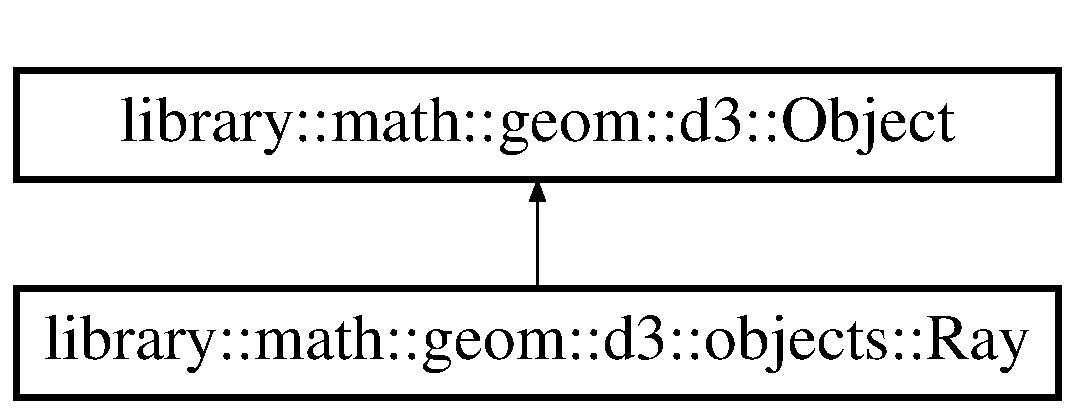
\includegraphics[height=2.000000cm]{classlibrary_1_1math_1_1geom_1_1d3_1_1objects_1_1_ray}
\end{center}
\end{figure}
\subsection*{Public Member Functions}
\begin{DoxyCompactItemize}
\item 
\hyperlink{classlibrary_1_1math_1_1geom_1_1d3_1_1objects_1_1_ray_a11b7613464daaebc6e25a758b057f203}{Ray} (const \hyperlink{classlibrary_1_1math_1_1geom_1_1d3_1_1objects_1_1_point}{Point} \&an\+Origin, const Vector3d \&a\+Direction)
\begin{DoxyCompactList}\small\item\em Constructor. \end{DoxyCompactList}\item 
virtual \hyperlink{classlibrary_1_1math_1_1geom_1_1d3_1_1objects_1_1_ray}{Ray} $\ast$ \hyperlink{classlibrary_1_1math_1_1geom_1_1d3_1_1objects_1_1_ray_a247ea36c39c3b44d003b157689850ae4}{clone} () const override
\begin{DoxyCompactList}\small\item\em Clone ray. \end{DoxyCompactList}\item 
bool \hyperlink{classlibrary_1_1math_1_1geom_1_1d3_1_1objects_1_1_ray_a90dbc4baa23e5f74b26b566bb862592f}{operator==} (const \hyperlink{classlibrary_1_1math_1_1geom_1_1d3_1_1objects_1_1_ray}{Ray} \&a\+Ray) const
\begin{DoxyCompactList}\small\item\em Equal to operator. \end{DoxyCompactList}\item 
bool \hyperlink{classlibrary_1_1math_1_1geom_1_1d3_1_1objects_1_1_ray_a0cd84346b37f62793b565c87ae4659fb}{operator!=} (const \hyperlink{classlibrary_1_1math_1_1geom_1_1d3_1_1objects_1_1_ray}{Ray} \&a\+Ray) const
\begin{DoxyCompactList}\small\item\em Not equal to operator. \end{DoxyCompactList}\item 
virtual bool \hyperlink{classlibrary_1_1math_1_1geom_1_1d3_1_1objects_1_1_ray_a7329f77a549a02e9c27d07c11adcc8bf}{is\+Defined} () const override
\begin{DoxyCompactList}\small\item\em Check if ray is defined. \end{DoxyCompactList}\item 
bool \hyperlink{classlibrary_1_1math_1_1geom_1_1d3_1_1objects_1_1_ray_a83300d3992b2f963c5b60a8be6748da0}{intersects} (const \hyperlink{classlibrary_1_1math_1_1geom_1_1d3_1_1objects_1_1_point}{Point} \&a\+Point) const
\begin{DoxyCompactList}\small\item\em Check if ray intersects point. \end{DoxyCompactList}\item 
bool \hyperlink{classlibrary_1_1math_1_1geom_1_1d3_1_1objects_1_1_ray_ade9febdb0da483a04f3a4d379c48b6d7}{intersects} (const \hyperlink{classlibrary_1_1math_1_1geom_1_1d3_1_1objects_1_1_plane}{Plane} \&a\+Plane) const
\begin{DoxyCompactList}\small\item\em Check if ray intersects plane. \end{DoxyCompactList}\item 
bool \hyperlink{classlibrary_1_1math_1_1geom_1_1d3_1_1objects_1_1_ray_ab75f38e9f6f0e7160acdf5360089937b}{intersects} (const \hyperlink{classlibrary_1_1math_1_1geom_1_1d3_1_1objects_1_1_sphere}{Sphere} \&a\+Sphere) const
\begin{DoxyCompactList}\small\item\em Check if ray intersects sphere. \end{DoxyCompactList}\item 
bool \hyperlink{classlibrary_1_1math_1_1geom_1_1d3_1_1objects_1_1_ray_a691d9fda5c22f8cef0b412b9173fe71b}{intersects} (const \hyperlink{classlibrary_1_1math_1_1geom_1_1d3_1_1objects_1_1_ellipsoid}{Ellipsoid} \&an\+Ellipsoid) const
\begin{DoxyCompactList}\small\item\em Check if ray intersects ellipsoid. \end{DoxyCompactList}\item 
bool \hyperlink{classlibrary_1_1math_1_1geom_1_1d3_1_1objects_1_1_ray_a6179dc1453ac7a54b13fe6bf46c0a66b}{contains} (const \hyperlink{classlibrary_1_1math_1_1geom_1_1d3_1_1objects_1_1_point}{Point} \&a\+Point) const
\begin{DoxyCompactList}\small\item\em Check if ray contains point. \end{DoxyCompactList}\item 
bool \hyperlink{classlibrary_1_1math_1_1geom_1_1d3_1_1objects_1_1_ray_a4766780e22a8113ff63b85c8af32e915}{contains} (const \hyperlink{classlibrary_1_1math_1_1geom_1_1d3_1_1objects_1_1_point_set}{Point\+Set} \&a\+Point\+Set) const
\begin{DoxyCompactList}\small\item\em Check if ray contains point set. \end{DoxyCompactList}\item 
\hyperlink{classlibrary_1_1math_1_1geom_1_1d3_1_1objects_1_1_point}{Point} \hyperlink{classlibrary_1_1math_1_1geom_1_1d3_1_1objects_1_1_ray_abaac9b7fcc10e2076ada11f2798386bd}{get\+Origin} () const
\begin{DoxyCompactList}\small\item\em Get ray origin. \end{DoxyCompactList}\item 
Vector3d \hyperlink{classlibrary_1_1math_1_1geom_1_1d3_1_1objects_1_1_ray_ab2e0a6cfd7c2c288ec615a479024fb7d}{get\+Direction} () const
\begin{DoxyCompactList}\small\item\em Get ray direction. \end{DoxyCompactList}\item 
\hyperlink{classlibrary_1_1math_1_1geom_1_1d3_1_1_intersection}{Intersection} \hyperlink{classlibrary_1_1math_1_1geom_1_1d3_1_1objects_1_1_ray_a50ede8e46490ec58931cb82754de873f}{intersection\+With} (const \hyperlink{classlibrary_1_1math_1_1geom_1_1d3_1_1objects_1_1_plane}{Plane} \&a\+Plane) const
\begin{DoxyCompactList}\small\item\em Compute intersection of ray with plane. \end{DoxyCompactList}\item 
\hyperlink{classlibrary_1_1math_1_1geom_1_1d3_1_1_intersection}{Intersection} \hyperlink{classlibrary_1_1math_1_1geom_1_1d3_1_1objects_1_1_ray_a54e7c2fa56bd086efbf85aa18674b403}{intersection\+With} (const \hyperlink{classlibrary_1_1math_1_1geom_1_1d3_1_1objects_1_1_sphere}{Sphere} \&a\+Sphere, const bool only\+In\+Sight=false) const
\begin{DoxyCompactList}\small\item\em Compute intersection of ray with sphere. \end{DoxyCompactList}\item 
\hyperlink{classlibrary_1_1math_1_1geom_1_1d3_1_1_intersection}{Intersection} \hyperlink{classlibrary_1_1math_1_1geom_1_1d3_1_1objects_1_1_ray_aea1460113fed4868d652c5f3bd7a9422}{intersection\+With} (const \hyperlink{classlibrary_1_1math_1_1geom_1_1d3_1_1objects_1_1_ellipsoid}{Ellipsoid} \&an\+Ellipsoid, const bool only\+In\+Sight=false) const
\begin{DoxyCompactList}\small\item\em Compute intersection of ray with ellipsoid. \end{DoxyCompactList}\item 
virtual void \hyperlink{classlibrary_1_1math_1_1geom_1_1d3_1_1objects_1_1_ray_a2140183dca4c36f5c51ed9e8f2cd220d}{print} (std\+::ostream \&an\+Output\+Stream, bool display\+Decorators=true) const override
\begin{DoxyCompactList}\small\item\em Print ray. \end{DoxyCompactList}\item 
virtual void \hyperlink{classlibrary_1_1math_1_1geom_1_1d3_1_1objects_1_1_ray_a0dd177a924978e1817a9fa888594e694}{apply\+Transformation} (const \hyperlink{classlibrary_1_1math_1_1geom_1_1d3_1_1_transformation}{Transformation} \&a\+Transformation) override
\begin{DoxyCompactList}\small\item\em Apply transformation to ray. \end{DoxyCompactList}\end{DoxyCompactItemize}
\subsection*{Static Public Member Functions}
\begin{DoxyCompactItemize}
\item 
static \hyperlink{classlibrary_1_1math_1_1geom_1_1d3_1_1objects_1_1_ray}{Ray} \hyperlink{classlibrary_1_1math_1_1geom_1_1d3_1_1objects_1_1_ray_abf40bfaeab9e9024fd1fc73893da09e0}{Undefined} ()
\begin{DoxyCompactList}\small\item\em Constructs an undefined ray. \end{DoxyCompactList}\end{DoxyCompactItemize}


\subsection{Detailed Description}
\hyperlink{classlibrary_1_1math_1_1geom_1_1d3_1_1objects_1_1_ray}{Ray}. 

https\+://en.wikipedia.\+org/wiki/\+Line\+\_\+(geometry)\hyperlink{classlibrary_1_1math_1_1geom_1_1d3_1_1objects_1_1_ray_a11b7613464daaebc6e25a758b057f203}{Ray} 

\subsection{Constructor \& Destructor Documentation}
\mbox{\Hypertarget{classlibrary_1_1math_1_1geom_1_1d3_1_1objects_1_1_ray_a11b7613464daaebc6e25a758b057f203}\label{classlibrary_1_1math_1_1geom_1_1d3_1_1objects_1_1_ray_a11b7613464daaebc6e25a758b057f203}} 
\index{library\+::math\+::geom\+::d3\+::objects\+::\+Ray@{library\+::math\+::geom\+::d3\+::objects\+::\+Ray}!Ray@{Ray}}
\index{Ray@{Ray}!library\+::math\+::geom\+::d3\+::objects\+::\+Ray@{library\+::math\+::geom\+::d3\+::objects\+::\+Ray}}
\subsubsection{\texorpdfstring{Ray()}{Ray()}}
{\footnotesize\ttfamily library\+::math\+::geom\+::d3\+::objects\+::\+Ray\+::\+Ray (\begin{DoxyParamCaption}\item[{const \hyperlink{classlibrary_1_1math_1_1geom_1_1d3_1_1objects_1_1_point}{Point} \&}]{an\+Origin,  }\item[{const Vector3d \&}]{a\+Direction }\end{DoxyParamCaption})}



Constructor. 


\begin{DoxyCode}
\hyperlink{classlibrary_1_1math_1_1geom_1_1d3_1_1objects_1_1_ray_a11b7613464daaebc6e25a758b057f203}{Ray} ray(\{ 0.0, 0.0, 0.0 \}, \{ 0.0, 0.0, 1.0 \}) ;
\end{DoxyCode}



\begin{DoxyParams}[1]{Parameters}
\mbox{\tt in}  & {\em an\+Origin} & A ray origin \\
\hline
\mbox{\tt in}  & {\em a\+Direction} & A ray direction \\
\hline
\end{DoxyParams}


\subsection{Member Function Documentation}
\mbox{\Hypertarget{classlibrary_1_1math_1_1geom_1_1d3_1_1objects_1_1_ray_a0dd177a924978e1817a9fa888594e694}\label{classlibrary_1_1math_1_1geom_1_1d3_1_1objects_1_1_ray_a0dd177a924978e1817a9fa888594e694}} 
\index{library\+::math\+::geom\+::d3\+::objects\+::\+Ray@{library\+::math\+::geom\+::d3\+::objects\+::\+Ray}!apply\+Transformation@{apply\+Transformation}}
\index{apply\+Transformation@{apply\+Transformation}!library\+::math\+::geom\+::d3\+::objects\+::\+Ray@{library\+::math\+::geom\+::d3\+::objects\+::\+Ray}}
\subsubsection{\texorpdfstring{apply\+Transformation()}{applyTransformation()}}
{\footnotesize\ttfamily void library\+::math\+::geom\+::d3\+::objects\+::\+Ray\+::apply\+Transformation (\begin{DoxyParamCaption}\item[{const \hyperlink{classlibrary_1_1math_1_1geom_1_1d3_1_1_transformation}{Transformation} \&}]{a\+Transformation }\end{DoxyParamCaption})\hspace{0.3cm}{\ttfamily [override]}, {\ttfamily [virtual]}}



Apply transformation to ray. 


\begin{DoxyParams}[1]{Parameters}
\mbox{\tt in}  & {\em a\+Transformation} & A transformation \\
\hline
\end{DoxyParams}


Implements \hyperlink{classlibrary_1_1math_1_1geom_1_1d3_1_1_object_a5fc47b1ee5d9a28efc6010d3d1512470}{library\+::math\+::geom\+::d3\+::\+Object}.

\mbox{\Hypertarget{classlibrary_1_1math_1_1geom_1_1d3_1_1objects_1_1_ray_a247ea36c39c3b44d003b157689850ae4}\label{classlibrary_1_1math_1_1geom_1_1d3_1_1objects_1_1_ray_a247ea36c39c3b44d003b157689850ae4}} 
\index{library\+::math\+::geom\+::d3\+::objects\+::\+Ray@{library\+::math\+::geom\+::d3\+::objects\+::\+Ray}!clone@{clone}}
\index{clone@{clone}!library\+::math\+::geom\+::d3\+::objects\+::\+Ray@{library\+::math\+::geom\+::d3\+::objects\+::\+Ray}}
\subsubsection{\texorpdfstring{clone()}{clone()}}
{\footnotesize\ttfamily \hyperlink{classlibrary_1_1math_1_1geom_1_1d3_1_1objects_1_1_ray}{Ray} $\ast$ library\+::math\+::geom\+::d3\+::objects\+::\+Ray\+::clone (\begin{DoxyParamCaption}{ }\end{DoxyParamCaption}) const\hspace{0.3cm}{\ttfamily [override]}, {\ttfamily [virtual]}}



Clone ray. 

\begin{DoxyReturn}{Returns}
Pointer to cloned ray 
\end{DoxyReturn}


Implements \hyperlink{classlibrary_1_1math_1_1geom_1_1d3_1_1_object_a1a784c6b359e0eb97cd34fabc42f2f3f}{library\+::math\+::geom\+::d3\+::\+Object}.

\mbox{\Hypertarget{classlibrary_1_1math_1_1geom_1_1d3_1_1objects_1_1_ray_a6179dc1453ac7a54b13fe6bf46c0a66b}\label{classlibrary_1_1math_1_1geom_1_1d3_1_1objects_1_1_ray_a6179dc1453ac7a54b13fe6bf46c0a66b}} 
\index{library\+::math\+::geom\+::d3\+::objects\+::\+Ray@{library\+::math\+::geom\+::d3\+::objects\+::\+Ray}!contains@{contains}}
\index{contains@{contains}!library\+::math\+::geom\+::d3\+::objects\+::\+Ray@{library\+::math\+::geom\+::d3\+::objects\+::\+Ray}}
\subsubsection{\texorpdfstring{contains()}{contains()}\hspace{0.1cm}{\footnotesize\ttfamily [1/2]}}
{\footnotesize\ttfamily bool library\+::math\+::geom\+::d3\+::objects\+::\+Ray\+::contains (\begin{DoxyParamCaption}\item[{const \hyperlink{classlibrary_1_1math_1_1geom_1_1d3_1_1objects_1_1_point}{Point} \&}]{a\+Point }\end{DoxyParamCaption}) const}



Check if ray contains point. 


\begin{DoxyCode}
\hyperlink{classlibrary_1_1math_1_1geom_1_1d3_1_1objects_1_1_ray_a11b7613464daaebc6e25a758b057f203}{Ray} ray = ... ;
Point point = ... ;
ray.contains(point) ;
\end{DoxyCode}



\begin{DoxyParams}[1]{Parameters}
\mbox{\tt in}  & {\em a\+Point} & A point \\
\hline
\end{DoxyParams}
\begin{DoxyReturn}{Returns}
True if ray contains point 
\end{DoxyReturn}
\mbox{\Hypertarget{classlibrary_1_1math_1_1geom_1_1d3_1_1objects_1_1_ray_a4766780e22a8113ff63b85c8af32e915}\label{classlibrary_1_1math_1_1geom_1_1d3_1_1objects_1_1_ray_a4766780e22a8113ff63b85c8af32e915}} 
\index{library\+::math\+::geom\+::d3\+::objects\+::\+Ray@{library\+::math\+::geom\+::d3\+::objects\+::\+Ray}!contains@{contains}}
\index{contains@{contains}!library\+::math\+::geom\+::d3\+::objects\+::\+Ray@{library\+::math\+::geom\+::d3\+::objects\+::\+Ray}}
\subsubsection{\texorpdfstring{contains()}{contains()}\hspace{0.1cm}{\footnotesize\ttfamily [2/2]}}
{\footnotesize\ttfamily bool library\+::math\+::geom\+::d3\+::objects\+::\+Ray\+::contains (\begin{DoxyParamCaption}\item[{const \hyperlink{classlibrary_1_1math_1_1geom_1_1d3_1_1objects_1_1_point_set}{Point\+Set} \&}]{a\+Point\+Set }\end{DoxyParamCaption}) const}



Check if ray contains point set. 


\begin{DoxyCode}
\hyperlink{classlibrary_1_1math_1_1geom_1_1d3_1_1objects_1_1_ray_a11b7613464daaebc6e25a758b057f203}{Ray} ray = ... ;
PointSet pointSet = ... ;
ray.contains(pointSet) ;
\end{DoxyCode}



\begin{DoxyParams}[1]{Parameters}
\mbox{\tt in}  & {\em a\+Point\+Set} & A point set \\
\hline
\end{DoxyParams}
\begin{DoxyReturn}{Returns}
True if ray contains point set 
\end{DoxyReturn}
\mbox{\Hypertarget{classlibrary_1_1math_1_1geom_1_1d3_1_1objects_1_1_ray_ab2e0a6cfd7c2c288ec615a479024fb7d}\label{classlibrary_1_1math_1_1geom_1_1d3_1_1objects_1_1_ray_ab2e0a6cfd7c2c288ec615a479024fb7d}} 
\index{library\+::math\+::geom\+::d3\+::objects\+::\+Ray@{library\+::math\+::geom\+::d3\+::objects\+::\+Ray}!get\+Direction@{get\+Direction}}
\index{get\+Direction@{get\+Direction}!library\+::math\+::geom\+::d3\+::objects\+::\+Ray@{library\+::math\+::geom\+::d3\+::objects\+::\+Ray}}
\subsubsection{\texorpdfstring{get\+Direction()}{getDirection()}}
{\footnotesize\ttfamily Vector3d library\+::math\+::geom\+::d3\+::objects\+::\+Ray\+::get\+Direction (\begin{DoxyParamCaption}{ }\end{DoxyParamCaption}) const}



Get ray direction. 


\begin{DoxyCode}
\hyperlink{classlibrary_1_1math_1_1geom_1_1d3_1_1objects_1_1_ray_a11b7613464daaebc6e25a758b057f203}{Ray}(\{ 0.0, 0.0, 0.0 \}, \{ 0.0, 0.0, 1.0 \}).\hyperlink{classlibrary_1_1math_1_1geom_1_1d3_1_1objects_1_1_ray_ab2e0a6cfd7c2c288ec615a479024fb7d}{getDirection}() ; \textcolor{comment}{// [0.0, 0.0, 1.0]}
\end{DoxyCode}


\begin{DoxyReturn}{Returns}
\hyperlink{classlibrary_1_1math_1_1geom_1_1d3_1_1objects_1_1_ray}{Ray} direction 
\end{DoxyReturn}
\mbox{\Hypertarget{classlibrary_1_1math_1_1geom_1_1d3_1_1objects_1_1_ray_abaac9b7fcc10e2076ada11f2798386bd}\label{classlibrary_1_1math_1_1geom_1_1d3_1_1objects_1_1_ray_abaac9b7fcc10e2076ada11f2798386bd}} 
\index{library\+::math\+::geom\+::d3\+::objects\+::\+Ray@{library\+::math\+::geom\+::d3\+::objects\+::\+Ray}!get\+Origin@{get\+Origin}}
\index{get\+Origin@{get\+Origin}!library\+::math\+::geom\+::d3\+::objects\+::\+Ray@{library\+::math\+::geom\+::d3\+::objects\+::\+Ray}}
\subsubsection{\texorpdfstring{get\+Origin()}{getOrigin()}}
{\footnotesize\ttfamily \hyperlink{classlibrary_1_1math_1_1geom_1_1d3_1_1objects_1_1_point}{Point} library\+::math\+::geom\+::d3\+::objects\+::\+Ray\+::get\+Origin (\begin{DoxyParamCaption}{ }\end{DoxyParamCaption}) const}



Get ray origin. 


\begin{DoxyCode}
\hyperlink{classlibrary_1_1math_1_1geom_1_1d3_1_1objects_1_1_ray_a11b7613464daaebc6e25a758b057f203}{Ray}(\{ 0.0, 0.0, 0.0 \}, \{ 0.0, 0.0, 1.0 \}).\hyperlink{classlibrary_1_1math_1_1geom_1_1d3_1_1objects_1_1_ray_abaac9b7fcc10e2076ada11f2798386bd}{getOrigin}() ; \textcolor{comment}{// [0.0, 0.0, 0.0]}
\end{DoxyCode}


\begin{DoxyReturn}{Returns}
\hyperlink{classlibrary_1_1math_1_1geom_1_1d3_1_1objects_1_1_ray}{Ray} origin 
\end{DoxyReturn}
\mbox{\Hypertarget{classlibrary_1_1math_1_1geom_1_1d3_1_1objects_1_1_ray_a50ede8e46490ec58931cb82754de873f}\label{classlibrary_1_1math_1_1geom_1_1d3_1_1objects_1_1_ray_a50ede8e46490ec58931cb82754de873f}} 
\index{library\+::math\+::geom\+::d3\+::objects\+::\+Ray@{library\+::math\+::geom\+::d3\+::objects\+::\+Ray}!intersection\+With@{intersection\+With}}
\index{intersection\+With@{intersection\+With}!library\+::math\+::geom\+::d3\+::objects\+::\+Ray@{library\+::math\+::geom\+::d3\+::objects\+::\+Ray}}
\subsubsection{\texorpdfstring{intersection\+With()}{intersectionWith()}\hspace{0.1cm}{\footnotesize\ttfamily [1/3]}}
{\footnotesize\ttfamily \hyperlink{classlibrary_1_1math_1_1geom_1_1d3_1_1_intersection}{Intersection} library\+::math\+::geom\+::d3\+::objects\+::\+Ray\+::intersection\+With (\begin{DoxyParamCaption}\item[{const \hyperlink{classlibrary_1_1math_1_1geom_1_1d3_1_1objects_1_1_plane}{Plane} \&}]{a\+Plane }\end{DoxyParamCaption}) const}



Compute intersection of ray with plane. 


\begin{DoxyParams}[1]{Parameters}
\mbox{\tt in}  & {\em a\+Plane} & A plane \\
\hline
\end{DoxyParams}
\begin{DoxyReturn}{Returns}
\hyperlink{classlibrary_1_1math_1_1geom_1_1d3_1_1_intersection}{Intersection} of ray with plane 
\end{DoxyReturn}
\mbox{\Hypertarget{classlibrary_1_1math_1_1geom_1_1d3_1_1objects_1_1_ray_a54e7c2fa56bd086efbf85aa18674b403}\label{classlibrary_1_1math_1_1geom_1_1d3_1_1objects_1_1_ray_a54e7c2fa56bd086efbf85aa18674b403}} 
\index{library\+::math\+::geom\+::d3\+::objects\+::\+Ray@{library\+::math\+::geom\+::d3\+::objects\+::\+Ray}!intersection\+With@{intersection\+With}}
\index{intersection\+With@{intersection\+With}!library\+::math\+::geom\+::d3\+::objects\+::\+Ray@{library\+::math\+::geom\+::d3\+::objects\+::\+Ray}}
\subsubsection{\texorpdfstring{intersection\+With()}{intersectionWith()}\hspace{0.1cm}{\footnotesize\ttfamily [2/3]}}
{\footnotesize\ttfamily \hyperlink{classlibrary_1_1math_1_1geom_1_1d3_1_1_intersection}{Intersection} library\+::math\+::geom\+::d3\+::objects\+::\+Ray\+::intersection\+With (\begin{DoxyParamCaption}\item[{const \hyperlink{classlibrary_1_1math_1_1geom_1_1d3_1_1objects_1_1_sphere}{Sphere} \&}]{a\+Sphere,  }\item[{const bool}]{only\+In\+Sight = {\ttfamily false} }\end{DoxyParamCaption}) const}



Compute intersection of ray with sphere. 


\begin{DoxyParams}[1]{Parameters}
\mbox{\tt in}  & {\em a\+Sphere} & A sphere \\
\hline
\mbox{\tt in}  & {\em only\+In\+Sight} & (optional) If true, only return intersection points that are in sight \\
\hline
\end{DoxyParams}
\begin{DoxyReturn}{Returns}
\hyperlink{classlibrary_1_1math_1_1geom_1_1d3_1_1_intersection}{Intersection} of ray with sphere 
\end{DoxyReturn}
\mbox{\Hypertarget{classlibrary_1_1math_1_1geom_1_1d3_1_1objects_1_1_ray_aea1460113fed4868d652c5f3bd7a9422}\label{classlibrary_1_1math_1_1geom_1_1d3_1_1objects_1_1_ray_aea1460113fed4868d652c5f3bd7a9422}} 
\index{library\+::math\+::geom\+::d3\+::objects\+::\+Ray@{library\+::math\+::geom\+::d3\+::objects\+::\+Ray}!intersection\+With@{intersection\+With}}
\index{intersection\+With@{intersection\+With}!library\+::math\+::geom\+::d3\+::objects\+::\+Ray@{library\+::math\+::geom\+::d3\+::objects\+::\+Ray}}
\subsubsection{\texorpdfstring{intersection\+With()}{intersectionWith()}\hspace{0.1cm}{\footnotesize\ttfamily [3/3]}}
{\footnotesize\ttfamily \hyperlink{classlibrary_1_1math_1_1geom_1_1d3_1_1_intersection}{Intersection} library\+::math\+::geom\+::d3\+::objects\+::\+Ray\+::intersection\+With (\begin{DoxyParamCaption}\item[{const \hyperlink{classlibrary_1_1math_1_1geom_1_1d3_1_1objects_1_1_ellipsoid}{Ellipsoid} \&}]{an\+Ellipsoid,  }\item[{const bool}]{only\+In\+Sight = {\ttfamily false} }\end{DoxyParamCaption}) const}



Compute intersection of ray with ellipsoid. 


\begin{DoxyParams}[1]{Parameters}
\mbox{\tt in}  & {\em an\+Ellipsoid} & An ellipsoid \\
\hline
\mbox{\tt in}  & {\em only\+In\+Sight} & (optional) If true, only return intersection points that are in sight \\
\hline
\end{DoxyParams}
\begin{DoxyReturn}{Returns}
\hyperlink{classlibrary_1_1math_1_1geom_1_1d3_1_1_intersection}{Intersection} of ray with ellipsoid 
\end{DoxyReturn}
\mbox{\Hypertarget{classlibrary_1_1math_1_1geom_1_1d3_1_1objects_1_1_ray_a83300d3992b2f963c5b60a8be6748da0}\label{classlibrary_1_1math_1_1geom_1_1d3_1_1objects_1_1_ray_a83300d3992b2f963c5b60a8be6748da0}} 
\index{library\+::math\+::geom\+::d3\+::objects\+::\+Ray@{library\+::math\+::geom\+::d3\+::objects\+::\+Ray}!intersects@{intersects}}
\index{intersects@{intersects}!library\+::math\+::geom\+::d3\+::objects\+::\+Ray@{library\+::math\+::geom\+::d3\+::objects\+::\+Ray}}
\subsubsection{\texorpdfstring{intersects()}{intersects()}\hspace{0.1cm}{\footnotesize\ttfamily [1/4]}}
{\footnotesize\ttfamily bool library\+::math\+::geom\+::d3\+::objects\+::\+Ray\+::intersects (\begin{DoxyParamCaption}\item[{const \hyperlink{classlibrary_1_1math_1_1geom_1_1d3_1_1objects_1_1_point}{Point} \&}]{a\+Point }\end{DoxyParamCaption}) const}



Check if ray intersects point. 


\begin{DoxyCode}
\hyperlink{classlibrary_1_1math_1_1geom_1_1d3_1_1objects_1_1_ray_a11b7613464daaebc6e25a758b057f203}{Ray} ray = ... ;
Point point = ... ;
ray.intersects(point) ;
\end{DoxyCode}



\begin{DoxyParams}[1]{Parameters}
\mbox{\tt in}  & {\em an\+Point} & A point \\
\hline
\end{DoxyParams}
\begin{DoxyReturn}{Returns}
True if ray intersects point 
\end{DoxyReturn}
\mbox{\Hypertarget{classlibrary_1_1math_1_1geom_1_1d3_1_1objects_1_1_ray_ade9febdb0da483a04f3a4d379c48b6d7}\label{classlibrary_1_1math_1_1geom_1_1d3_1_1objects_1_1_ray_ade9febdb0da483a04f3a4d379c48b6d7}} 
\index{library\+::math\+::geom\+::d3\+::objects\+::\+Ray@{library\+::math\+::geom\+::d3\+::objects\+::\+Ray}!intersects@{intersects}}
\index{intersects@{intersects}!library\+::math\+::geom\+::d3\+::objects\+::\+Ray@{library\+::math\+::geom\+::d3\+::objects\+::\+Ray}}
\subsubsection{\texorpdfstring{intersects()}{intersects()}\hspace{0.1cm}{\footnotesize\ttfamily [2/4]}}
{\footnotesize\ttfamily bool library\+::math\+::geom\+::d3\+::objects\+::\+Ray\+::intersects (\begin{DoxyParamCaption}\item[{const \hyperlink{classlibrary_1_1math_1_1geom_1_1d3_1_1objects_1_1_plane}{Plane} \&}]{a\+Plane }\end{DoxyParamCaption}) const}



Check if ray intersects plane. 


\begin{DoxyCode}
\hyperlink{classlibrary_1_1math_1_1geom_1_1d3_1_1objects_1_1_ray_a11b7613464daaebc6e25a758b057f203}{Ray} ray = ... ;
Plane plane = ... ;
ray.intersects(plane) ;
\end{DoxyCode}



\begin{DoxyParams}[1]{Parameters}
\mbox{\tt in}  & {\em a\+Plane} & A plane \\
\hline
\end{DoxyParams}
\begin{DoxyReturn}{Returns}
True if ray intersects plane 
\end{DoxyReturn}
\mbox{\Hypertarget{classlibrary_1_1math_1_1geom_1_1d3_1_1objects_1_1_ray_ab75f38e9f6f0e7160acdf5360089937b}\label{classlibrary_1_1math_1_1geom_1_1d3_1_1objects_1_1_ray_ab75f38e9f6f0e7160acdf5360089937b}} 
\index{library\+::math\+::geom\+::d3\+::objects\+::\+Ray@{library\+::math\+::geom\+::d3\+::objects\+::\+Ray}!intersects@{intersects}}
\index{intersects@{intersects}!library\+::math\+::geom\+::d3\+::objects\+::\+Ray@{library\+::math\+::geom\+::d3\+::objects\+::\+Ray}}
\subsubsection{\texorpdfstring{intersects()}{intersects()}\hspace{0.1cm}{\footnotesize\ttfamily [3/4]}}
{\footnotesize\ttfamily bool library\+::math\+::geom\+::d3\+::objects\+::\+Ray\+::intersects (\begin{DoxyParamCaption}\item[{const \hyperlink{classlibrary_1_1math_1_1geom_1_1d3_1_1objects_1_1_sphere}{Sphere} \&}]{a\+Sphere }\end{DoxyParamCaption}) const}



Check if ray intersects sphere. 


\begin{DoxyCode}
\hyperlink{classlibrary_1_1math_1_1geom_1_1d3_1_1objects_1_1_ray_a11b7613464daaebc6e25a758b057f203}{Ray} ray = ... ;
Sphere sphere = ... ;
ray.intersects(sphere) ;
\end{DoxyCode}



\begin{DoxyParams}[1]{Parameters}
\mbox{\tt in}  & {\em an\+Sphere} & A sphere \\
\hline
\end{DoxyParams}
\begin{DoxyReturn}{Returns}
True if ray intersects sphere 
\end{DoxyReturn}
\mbox{\Hypertarget{classlibrary_1_1math_1_1geom_1_1d3_1_1objects_1_1_ray_a691d9fda5c22f8cef0b412b9173fe71b}\label{classlibrary_1_1math_1_1geom_1_1d3_1_1objects_1_1_ray_a691d9fda5c22f8cef0b412b9173fe71b}} 
\index{library\+::math\+::geom\+::d3\+::objects\+::\+Ray@{library\+::math\+::geom\+::d3\+::objects\+::\+Ray}!intersects@{intersects}}
\index{intersects@{intersects}!library\+::math\+::geom\+::d3\+::objects\+::\+Ray@{library\+::math\+::geom\+::d3\+::objects\+::\+Ray}}
\subsubsection{\texorpdfstring{intersects()}{intersects()}\hspace{0.1cm}{\footnotesize\ttfamily [4/4]}}
{\footnotesize\ttfamily bool library\+::math\+::geom\+::d3\+::objects\+::\+Ray\+::intersects (\begin{DoxyParamCaption}\item[{const \hyperlink{classlibrary_1_1math_1_1geom_1_1d3_1_1objects_1_1_ellipsoid}{Ellipsoid} \&}]{an\+Ellipsoid }\end{DoxyParamCaption}) const}



Check if ray intersects ellipsoid. 


\begin{DoxyCode}
\hyperlink{classlibrary_1_1math_1_1geom_1_1d3_1_1objects_1_1_ray_a11b7613464daaebc6e25a758b057f203}{Ray} ray = ... ;
Ellipsoid ellipsoid = ... ;
ray.intersects(ellipsoid) ;
\end{DoxyCode}



\begin{DoxyParams}[1]{Parameters}
\mbox{\tt in}  & {\em an\+Ellipsoid} & An ellipsoid \\
\hline
\end{DoxyParams}
\begin{DoxyReturn}{Returns}
True if ray intersects ellipsoid 
\end{DoxyReturn}
\mbox{\Hypertarget{classlibrary_1_1math_1_1geom_1_1d3_1_1objects_1_1_ray_a7329f77a549a02e9c27d07c11adcc8bf}\label{classlibrary_1_1math_1_1geom_1_1d3_1_1objects_1_1_ray_a7329f77a549a02e9c27d07c11adcc8bf}} 
\index{library\+::math\+::geom\+::d3\+::objects\+::\+Ray@{library\+::math\+::geom\+::d3\+::objects\+::\+Ray}!is\+Defined@{is\+Defined}}
\index{is\+Defined@{is\+Defined}!library\+::math\+::geom\+::d3\+::objects\+::\+Ray@{library\+::math\+::geom\+::d3\+::objects\+::\+Ray}}
\subsubsection{\texorpdfstring{is\+Defined()}{isDefined()}}
{\footnotesize\ttfamily bool library\+::math\+::geom\+::d3\+::objects\+::\+Ray\+::is\+Defined (\begin{DoxyParamCaption}{ }\end{DoxyParamCaption}) const\hspace{0.3cm}{\ttfamily [override]}, {\ttfamily [virtual]}}



Check if ray is defined. 


\begin{DoxyCode}
\hyperlink{classlibrary_1_1math_1_1geom_1_1d3_1_1objects_1_1_ray_a11b7613464daaebc6e25a758b057f203}{Ray}(\{ 0.0, 0.0, 0.0 \}, \{ 0.0, 0.0, 1.0 \}).\hyperlink{classlibrary_1_1math_1_1geom_1_1d3_1_1objects_1_1_ray_a7329f77a549a02e9c27d07c11adcc8bf}{isDefined}() ; \textcolor{comment}{// True}
\end{DoxyCode}


\begin{DoxyReturn}{Returns}
True if ray is defined 
\end{DoxyReturn}


Implements \hyperlink{classlibrary_1_1math_1_1geom_1_1d3_1_1_object_a2216442e322f0c3ca5f01a4efa22baf7}{library\+::math\+::geom\+::d3\+::\+Object}.

\mbox{\Hypertarget{classlibrary_1_1math_1_1geom_1_1d3_1_1objects_1_1_ray_a0cd84346b37f62793b565c87ae4659fb}\label{classlibrary_1_1math_1_1geom_1_1d3_1_1objects_1_1_ray_a0cd84346b37f62793b565c87ae4659fb}} 
\index{library\+::math\+::geom\+::d3\+::objects\+::\+Ray@{library\+::math\+::geom\+::d3\+::objects\+::\+Ray}!operator"!=@{operator"!=}}
\index{operator"!=@{operator"!=}!library\+::math\+::geom\+::d3\+::objects\+::\+Ray@{library\+::math\+::geom\+::d3\+::objects\+::\+Ray}}
\subsubsection{\texorpdfstring{operator"!=()}{operator!=()}}
{\footnotesize\ttfamily bool library\+::math\+::geom\+::d3\+::objects\+::\+Ray\+::operator!= (\begin{DoxyParamCaption}\item[{const \hyperlink{classlibrary_1_1math_1_1geom_1_1d3_1_1objects_1_1_ray}{Ray} \&}]{a\+Ray }\end{DoxyParamCaption}) const}



Not equal to operator. 


\begin{DoxyCode}
\hyperlink{classlibrary_1_1math_1_1geom_1_1d3_1_1objects_1_1_ray_a11b7613464daaebc6e25a758b057f203}{Ray}(\{ 0.0, 0.0, 0.0 \}, \{ 0.0, 0.0, 1.0 \}) != \hyperlink{classlibrary_1_1math_1_1geom_1_1d3_1_1objects_1_1_ray_a11b7613464daaebc6e25a758b057f203}{Ray}(\{ 0.0, 0.0, 0.0 \}, \{ 0.0, 0.0, 2.0 \}) ; \textcolor{comment}{// True}
\end{DoxyCode}



\begin{DoxyParams}[1]{Parameters}
\mbox{\tt in}  & {\em a\+Ray} & A ray \\
\hline
\end{DoxyParams}
\begin{DoxyReturn}{Returns}
True if rays are not equal 
\end{DoxyReturn}
\mbox{\Hypertarget{classlibrary_1_1math_1_1geom_1_1d3_1_1objects_1_1_ray_a90dbc4baa23e5f74b26b566bb862592f}\label{classlibrary_1_1math_1_1geom_1_1d3_1_1objects_1_1_ray_a90dbc4baa23e5f74b26b566bb862592f}} 
\index{library\+::math\+::geom\+::d3\+::objects\+::\+Ray@{library\+::math\+::geom\+::d3\+::objects\+::\+Ray}!operator==@{operator==}}
\index{operator==@{operator==}!library\+::math\+::geom\+::d3\+::objects\+::\+Ray@{library\+::math\+::geom\+::d3\+::objects\+::\+Ray}}
\subsubsection{\texorpdfstring{operator==()}{operator==()}}
{\footnotesize\ttfamily bool library\+::math\+::geom\+::d3\+::objects\+::\+Ray\+::operator== (\begin{DoxyParamCaption}\item[{const \hyperlink{classlibrary_1_1math_1_1geom_1_1d3_1_1objects_1_1_ray}{Ray} \&}]{a\+Ray }\end{DoxyParamCaption}) const}



Equal to operator. 


\begin{DoxyCode}
\hyperlink{classlibrary_1_1math_1_1geom_1_1d3_1_1objects_1_1_ray_a11b7613464daaebc6e25a758b057f203}{Ray}(\{ 0.0, 0.0, 0.0 \}, \{ 0.0, 0.0, 1.0 \}) == \hyperlink{classlibrary_1_1math_1_1geom_1_1d3_1_1objects_1_1_ray_a11b7613464daaebc6e25a758b057f203}{Ray}(\{ 0.0, 0.0, 0.0 \}, \{ 0.0, 0.0, 1.0 \}) ; \textcolor{comment}{// True}
\end{DoxyCode}



\begin{DoxyParams}[1]{Parameters}
\mbox{\tt in}  & {\em a\+Ray} & A ray \\
\hline
\end{DoxyParams}
\begin{DoxyReturn}{Returns}
True if rays are equal 
\end{DoxyReturn}
\mbox{\Hypertarget{classlibrary_1_1math_1_1geom_1_1d3_1_1objects_1_1_ray_a2140183dca4c36f5c51ed9e8f2cd220d}\label{classlibrary_1_1math_1_1geom_1_1d3_1_1objects_1_1_ray_a2140183dca4c36f5c51ed9e8f2cd220d}} 
\index{library\+::math\+::geom\+::d3\+::objects\+::\+Ray@{library\+::math\+::geom\+::d3\+::objects\+::\+Ray}!print@{print}}
\index{print@{print}!library\+::math\+::geom\+::d3\+::objects\+::\+Ray@{library\+::math\+::geom\+::d3\+::objects\+::\+Ray}}
\subsubsection{\texorpdfstring{print()}{print()}}
{\footnotesize\ttfamily void library\+::math\+::geom\+::d3\+::objects\+::\+Ray\+::print (\begin{DoxyParamCaption}\item[{std\+::ostream \&}]{an\+Output\+Stream,  }\item[{bool}]{display\+Decorators = {\ttfamily true} }\end{DoxyParamCaption}) const\hspace{0.3cm}{\ttfamily [override]}, {\ttfamily [virtual]}}



Print ray. 


\begin{DoxyParams}[1]{Parameters}
\mbox{\tt in}  & {\em an\+Output\+Stream} & An output stream \\
\hline
\mbox{\tt in}  & {\em (optional)} & display\+Decorators If true, display decorators \\
\hline
\end{DoxyParams}


Implements \hyperlink{classlibrary_1_1math_1_1geom_1_1d3_1_1_object_aa166f4ce4d116a248f0fc861c75012ca}{library\+::math\+::geom\+::d3\+::\+Object}.

\mbox{\Hypertarget{classlibrary_1_1math_1_1geom_1_1d3_1_1objects_1_1_ray_abf40bfaeab9e9024fd1fc73893da09e0}\label{classlibrary_1_1math_1_1geom_1_1d3_1_1objects_1_1_ray_abf40bfaeab9e9024fd1fc73893da09e0}} 
\index{library\+::math\+::geom\+::d3\+::objects\+::\+Ray@{library\+::math\+::geom\+::d3\+::objects\+::\+Ray}!Undefined@{Undefined}}
\index{Undefined@{Undefined}!library\+::math\+::geom\+::d3\+::objects\+::\+Ray@{library\+::math\+::geom\+::d3\+::objects\+::\+Ray}}
\subsubsection{\texorpdfstring{Undefined()}{Undefined()}}
{\footnotesize\ttfamily \hyperlink{classlibrary_1_1math_1_1geom_1_1d3_1_1objects_1_1_ray}{Ray} library\+::math\+::geom\+::d3\+::objects\+::\+Ray\+::\+Undefined (\begin{DoxyParamCaption}{ }\end{DoxyParamCaption})\hspace{0.3cm}{\ttfamily [static]}}



Constructs an undefined ray. 


\begin{DoxyCode}
\hyperlink{classlibrary_1_1math_1_1geom_1_1d3_1_1objects_1_1_ray_a11b7613464daaebc6e25a758b057f203}{Ray} ray = \hyperlink{classlibrary_1_1math_1_1geom_1_1d3_1_1objects_1_1_ray_abf40bfaeab9e9024fd1fc73893da09e0}{Ray::Undefined}() ; \textcolor{comment}{// Undefined}
\end{DoxyCode}


\begin{DoxyReturn}{Returns}
Undefined ray 
\end{DoxyReturn}


The documentation for this class was generated from the following files\+:\begin{DoxyCompactItemize}
\item 
include/\+Library/\+Mathematics/\+Geometry/3\+D/\+Objects/\hyperlink{_ray_8hpp}{Ray.\+hpp}\item 
src/\+Library/\+Mathematics/\+Geometry/3\+D/\+Objects/\hyperlink{_ray_8cpp}{Ray.\+cpp}\end{DoxyCompactItemize}

\hypertarget{classlibrary_1_1math_1_1geom_1_1d3_1_1trf_1_1rot_1_1_rotation_matrix}{}\section{library\+:\+:math\+:\+:geom\+:\+:d3\+:\+:trf\+:\+:rot\+:\+:Rotation\+Matrix Class Reference}
\label{classlibrary_1_1math_1_1geom_1_1d3_1_1trf_1_1rot_1_1_rotation_matrix}\index{library\+::math\+::geom\+::d3\+::trf\+::rot\+::\+Rotation\+Matrix@{library\+::math\+::geom\+::d3\+::trf\+::rot\+::\+Rotation\+Matrix}}


Rotation matrix.  




{\ttfamily \#include $<$Rotation\+Matrix.\+hpp$>$}

\subsection*{Public Member Functions}
\begin{DoxyCompactItemize}
\item 
\hyperlink{classlibrary_1_1math_1_1geom_1_1d3_1_1trf_1_1rot_1_1_rotation_matrix_a7f1184694020cb4f963d58931324ab06}{Rotation\+Matrix} (const Matrix3d \&a\+Matrix)
\begin{DoxyCompactList}\small\item\em Constructor. \end{DoxyCompactList}\item 
\hyperlink{classlibrary_1_1math_1_1geom_1_1d3_1_1trf_1_1rot_1_1_rotation_matrix_a7618d97ef4861054a071a3431176c3a1}{Rotation\+Matrix} (const Real \&a\+First\+Coefficient, const Real \&a\+Second\+Coefficient, const Real \&a\+Third\+Coefficient, const Real \&a\+Fourth\+Coefficient, const Real \&a\+Fifth\+Coefficient, const Real \&a\+Sixth\+Coefficient, const Real \&a\+Seventh\+Coefficient, const Real \&a\+Eighth\+Coefficient, const Real \&a\+Ninth\+Coefficient)
\begin{DoxyCompactList}\small\item\em Constructor. \end{DoxyCompactList}\item 
bool \hyperlink{classlibrary_1_1math_1_1geom_1_1d3_1_1trf_1_1rot_1_1_rotation_matrix_adb54de25b2dbdd55ecd6d122f47b5996}{operator==} (const \hyperlink{classlibrary_1_1math_1_1geom_1_1d3_1_1trf_1_1rot_1_1_rotation_matrix}{Rotation\+Matrix} \&a\+Rotation\+Matrix) const
\begin{DoxyCompactList}\small\item\em Equal to operator. \end{DoxyCompactList}\item 
bool \hyperlink{classlibrary_1_1math_1_1geom_1_1d3_1_1trf_1_1rot_1_1_rotation_matrix_a7aabde35abe3bf30b5f38ab986e64f34}{operator!=} (const \hyperlink{classlibrary_1_1math_1_1geom_1_1d3_1_1trf_1_1rot_1_1_rotation_matrix}{Rotation\+Matrix} \&a\+Rotation\+Matrix) const
\begin{DoxyCompactList}\small\item\em Not equal to operator. \end{DoxyCompactList}\item 
\hyperlink{classlibrary_1_1math_1_1geom_1_1d3_1_1trf_1_1rot_1_1_rotation_matrix}{Rotation\+Matrix} \hyperlink{classlibrary_1_1math_1_1geom_1_1d3_1_1trf_1_1rot_1_1_rotation_matrix_aa3b9e906bba954c71fd54b2cadfea46f}{operator$\ast$} (const \hyperlink{classlibrary_1_1math_1_1geom_1_1d3_1_1trf_1_1rot_1_1_rotation_matrix}{Rotation\+Matrix} \&a\+Rotation\+Matrix) const
\begin{DoxyCompactList}\small\item\em Matrix multiplication operator. \end{DoxyCompactList}\item 
Vector3d \hyperlink{classlibrary_1_1math_1_1geom_1_1d3_1_1trf_1_1rot_1_1_rotation_matrix_a1b21bbea44cea009ae0533e206b202ff}{operator$\ast$} (const Vector3d \&a\+Vector) const
\begin{DoxyCompactList}\small\item\em Vector multiplication operator. \end{DoxyCompactList}\item 
double \hyperlink{classlibrary_1_1math_1_1geom_1_1d3_1_1trf_1_1rot_1_1_rotation_matrix_ad4a32ff81978cb60f2034661ea00d390}{operator()} (const Index \&a\+Row\+Index, const Index \&a\+Column\+Index) const
\begin{DoxyCompactList}\small\item\em Index function operator. \end{DoxyCompactList}\item 
double \& \hyperlink{classlibrary_1_1math_1_1geom_1_1d3_1_1trf_1_1rot_1_1_rotation_matrix_a2b6c7d6fe4770c59f2e1bc369798a36a}{operator()} (const Index \&a\+Row\+Index, const Index \&a\+Column\+Index)
\begin{DoxyCompactList}\small\item\em Index function operator. \end{DoxyCompactList}\item 
bool \hyperlink{classlibrary_1_1math_1_1geom_1_1d3_1_1trf_1_1rot_1_1_rotation_matrix_a8a3cb48f3cda99de31c763295030ffcc}{is\+Defined} () const
\begin{DoxyCompactList}\small\item\em Check if rotation matrix is defined. \end{DoxyCompactList}\item 
const Matrix3d \& \hyperlink{classlibrary_1_1math_1_1geom_1_1d3_1_1trf_1_1rot_1_1_rotation_matrix_a32eda074386b31ef093b33c960361276}{access\+Matrix} () const
\begin{DoxyCompactList}\small\item\em Access underlying rotation matrix. \end{DoxyCompactList}\item 
Vector3d \hyperlink{classlibrary_1_1math_1_1geom_1_1d3_1_1trf_1_1rot_1_1_rotation_matrix_a0eedb1df4a290e649486c1d7b0a8fba9}{get\+Row\+At} (const Index \&a\+Row\+Index) const
\begin{DoxyCompactList}\small\item\em Get row at index. \end{DoxyCompactList}\item 
Vector3d \hyperlink{classlibrary_1_1math_1_1geom_1_1d3_1_1trf_1_1rot_1_1_rotation_matrix_a020c6a8fd9b9c680908071b57b2a3422}{get\+Column\+At} (const Index \&a\+Column\+Index) const
\begin{DoxyCompactList}\small\item\em Get column at index. \end{DoxyCompactList}\item 
Matrix3d \hyperlink{classlibrary_1_1math_1_1geom_1_1d3_1_1trf_1_1rot_1_1_rotation_matrix_a374f061f73921d59caf9ce7c18ff0d91}{get\+Matrix} () const
\begin{DoxyCompactList}\small\item\em Get underlying rotation matrix. \end{DoxyCompactList}\item 
\hyperlink{classlibrary_1_1math_1_1geom_1_1d3_1_1trf_1_1rot_1_1_rotation_matrix}{Rotation\+Matrix} \hyperlink{classlibrary_1_1math_1_1geom_1_1d3_1_1trf_1_1rot_1_1_rotation_matrix_a42f35e00e2820b2d882e6abe494f8350}{to\+Transposed} () const
\begin{DoxyCompactList}\small\item\em Get transposed rotation matrix. \end{DoxyCompactList}\item 
\hyperlink{classlibrary_1_1math_1_1geom_1_1d3_1_1trf_1_1rot_1_1_rotation_matrix}{Rotation\+Matrix} \& \hyperlink{classlibrary_1_1math_1_1geom_1_1d3_1_1trf_1_1rot_1_1_rotation_matrix_a38307ba9d313c524745396338563be04}{transpose} ()
\begin{DoxyCompactList}\small\item\em Transpose rotation matrix. \end{DoxyCompactList}\end{DoxyCompactItemize}
\subsection*{Static Public Member Functions}
\begin{DoxyCompactItemize}
\item 
static \hyperlink{classlibrary_1_1math_1_1geom_1_1d3_1_1trf_1_1rot_1_1_rotation_matrix}{Rotation\+Matrix} \hyperlink{classlibrary_1_1math_1_1geom_1_1d3_1_1trf_1_1rot_1_1_rotation_matrix_a959b34738200815ce55874c17ea6b7a6}{Undefined} ()
\begin{DoxyCompactList}\small\item\em Constructs an undefined rotation matrix. \end{DoxyCompactList}\item 
static \hyperlink{classlibrary_1_1math_1_1geom_1_1d3_1_1trf_1_1rot_1_1_rotation_matrix}{Rotation\+Matrix} \hyperlink{classlibrary_1_1math_1_1geom_1_1d3_1_1trf_1_1rot_1_1_rotation_matrix_aeb5324151ee55348fa16c5fe78b036ed}{Unit} ()
\begin{DoxyCompactList}\small\item\em Constructs a unit rotation matrix. \end{DoxyCompactList}\item 
static \hyperlink{classlibrary_1_1math_1_1geom_1_1d3_1_1trf_1_1rot_1_1_rotation_matrix}{Rotation\+Matrix} \hyperlink{classlibrary_1_1math_1_1geom_1_1d3_1_1trf_1_1rot_1_1_rotation_matrix_a69fee7be102205645581ed5d26c90b21}{RX} (const \hyperlink{classlibrary_1_1math_1_1geom_1_1_angle}{Angle} \&a\+Rotation\+Angle)
\begin{DoxyCompactList}\small\item\em Constructs a rotation matrix representing a rotation around the X-\/axis. \end{DoxyCompactList}\item 
static \hyperlink{classlibrary_1_1math_1_1geom_1_1d3_1_1trf_1_1rot_1_1_rotation_matrix}{Rotation\+Matrix} \hyperlink{classlibrary_1_1math_1_1geom_1_1d3_1_1trf_1_1rot_1_1_rotation_matrix_a4aa94a9e709365c4beeeb011be81a5fb}{RY} (const \hyperlink{classlibrary_1_1math_1_1geom_1_1_angle}{Angle} \&a\+Rotation\+Angle)
\begin{DoxyCompactList}\small\item\em Constructs a rotation matrix representing a rotation around the Y-\/axis. \end{DoxyCompactList}\item 
static \hyperlink{classlibrary_1_1math_1_1geom_1_1d3_1_1trf_1_1rot_1_1_rotation_matrix}{Rotation\+Matrix} \hyperlink{classlibrary_1_1math_1_1geom_1_1d3_1_1trf_1_1rot_1_1_rotation_matrix_afc63f5b893d8c0024a0ba5c2ed69ab1b}{RZ} (const \hyperlink{classlibrary_1_1math_1_1geom_1_1_angle}{Angle} \&a\+Rotation\+Angle)
\begin{DoxyCompactList}\small\item\em Constructs a rotation matrix representing a rotation around the Z-\/axis. \end{DoxyCompactList}\item 
static \hyperlink{classlibrary_1_1math_1_1geom_1_1d3_1_1trf_1_1rot_1_1_rotation_matrix}{Rotation\+Matrix} \hyperlink{classlibrary_1_1math_1_1geom_1_1d3_1_1trf_1_1rot_1_1_rotation_matrix_aea3e4db9fb93537a0da28e2d50b62a66}{Rows} (const Vector3d \&a\+First\+Row, const Vector3d \&a\+Second\+Row, const Vector3d \&a\+Third\+Row)
\begin{DoxyCompactList}\small\item\em Constructs a rotation matrix from row vectors. \end{DoxyCompactList}\item 
static \hyperlink{classlibrary_1_1math_1_1geom_1_1d3_1_1trf_1_1rot_1_1_rotation_matrix}{Rotation\+Matrix} \hyperlink{classlibrary_1_1math_1_1geom_1_1d3_1_1trf_1_1rot_1_1_rotation_matrix_a73c73c91145a6b543801f41286f4a517}{Columns} (const Vector3d \&a\+First\+Column, const Vector3d \&a\+Second\+Column, const Vector3d \&a\+Third\+Column)
\begin{DoxyCompactList}\small\item\em Constructs a rotation matrix from column vectors. \end{DoxyCompactList}\item 
static \hyperlink{classlibrary_1_1math_1_1geom_1_1d3_1_1trf_1_1rot_1_1_rotation_matrix}{Rotation\+Matrix} \hyperlink{classlibrary_1_1math_1_1geom_1_1d3_1_1trf_1_1rot_1_1_rotation_matrix_a55511f2734e537277092905958d56d23}{Quaternion} (const \hyperlink{classlibrary_1_1math_1_1geom_1_1d3_1_1trf_1_1rot_1_1_quaternion}{rot\+::\+Quaternion} \&a\+Quaternion)
\begin{DoxyCompactList}\small\item\em Constructs a rotation matrix from a quaternion. \end{DoxyCompactList}\item 
static \hyperlink{classlibrary_1_1math_1_1geom_1_1d3_1_1trf_1_1rot_1_1_rotation_matrix}{Rotation\+Matrix} \hyperlink{classlibrary_1_1math_1_1geom_1_1d3_1_1trf_1_1rot_1_1_rotation_matrix_a1f7367f6d38b55e05623df62a8ea0be4}{Rotation\+Vector} (const \hyperlink{classlibrary_1_1math_1_1geom_1_1d3_1_1trf_1_1rot_1_1_rotation_vector}{rot\+::\+Rotation\+Vector} \&a\+Rotation\+Vector)
\begin{DoxyCompactList}\small\item\em Constructs a rotation matrix from a rotation vector. \end{DoxyCompactList}\end{DoxyCompactItemize}
\subsection*{Friends}
\begin{DoxyCompactItemize}
\item 
std\+::ostream \& \hyperlink{classlibrary_1_1math_1_1geom_1_1d3_1_1trf_1_1rot_1_1_rotation_matrix_aa9ed0897a6219331deeb7750017a0df9}{operator$<$$<$} (std\+::ostream \&an\+Output\+Stream, const \hyperlink{classlibrary_1_1math_1_1geom_1_1d3_1_1trf_1_1rot_1_1_rotation_matrix}{Rotation\+Matrix} \&a\+Rotation\+Matrix)
\begin{DoxyCompactList}\small\item\em Output stream operator. \end{DoxyCompactList}\end{DoxyCompactItemize}


\subsection{Detailed Description}
Rotation matrix. 

https\+://en.wikipedia.\+org/wiki/\+Rotation\+\_\+matrix 

\subsection{Constructor \& Destructor Documentation}
\mbox{\Hypertarget{classlibrary_1_1math_1_1geom_1_1d3_1_1trf_1_1rot_1_1_rotation_matrix_a7f1184694020cb4f963d58931324ab06}\label{classlibrary_1_1math_1_1geom_1_1d3_1_1trf_1_1rot_1_1_rotation_matrix_a7f1184694020cb4f963d58931324ab06}} 
\index{library\+::math\+::geom\+::d3\+::trf\+::rot\+::\+Rotation\+Matrix@{library\+::math\+::geom\+::d3\+::trf\+::rot\+::\+Rotation\+Matrix}!Rotation\+Matrix@{Rotation\+Matrix}}
\index{Rotation\+Matrix@{Rotation\+Matrix}!library\+::math\+::geom\+::d3\+::trf\+::rot\+::\+Rotation\+Matrix@{library\+::math\+::geom\+::d3\+::trf\+::rot\+::\+Rotation\+Matrix}}
\subsubsection{\texorpdfstring{Rotation\+Matrix()}{RotationMatrix()}\hspace{0.1cm}{\footnotesize\ttfamily [1/2]}}
{\footnotesize\ttfamily library\+::math\+::geom\+::d3\+::trf\+::rot\+::\+Rotation\+Matrix\+::\+Rotation\+Matrix (\begin{DoxyParamCaption}\item[{const Matrix3d \&}]{a\+Matrix }\end{DoxyParamCaption})}



Constructor. 


\begin{DoxyParams}[1]{Parameters}
\mbox{\tt in}  & {\em a\+Matrix} & A matrix \\
\hline
\end{DoxyParams}
\mbox{\Hypertarget{classlibrary_1_1math_1_1geom_1_1d3_1_1trf_1_1rot_1_1_rotation_matrix_a7618d97ef4861054a071a3431176c3a1}\label{classlibrary_1_1math_1_1geom_1_1d3_1_1trf_1_1rot_1_1_rotation_matrix_a7618d97ef4861054a071a3431176c3a1}} 
\index{library\+::math\+::geom\+::d3\+::trf\+::rot\+::\+Rotation\+Matrix@{library\+::math\+::geom\+::d3\+::trf\+::rot\+::\+Rotation\+Matrix}!Rotation\+Matrix@{Rotation\+Matrix}}
\index{Rotation\+Matrix@{Rotation\+Matrix}!library\+::math\+::geom\+::d3\+::trf\+::rot\+::\+Rotation\+Matrix@{library\+::math\+::geom\+::d3\+::trf\+::rot\+::\+Rotation\+Matrix}}
\subsubsection{\texorpdfstring{Rotation\+Matrix()}{RotationMatrix()}\hspace{0.1cm}{\footnotesize\ttfamily [2/2]}}
{\footnotesize\ttfamily library\+::math\+::geom\+::d3\+::trf\+::rot\+::\+Rotation\+Matrix\+::\+Rotation\+Matrix (\begin{DoxyParamCaption}\item[{const Real \&}]{a\+First\+Coefficient,  }\item[{const Real \&}]{a\+Second\+Coefficient,  }\item[{const Real \&}]{a\+Third\+Coefficient,  }\item[{const Real \&}]{a\+Fourth\+Coefficient,  }\item[{const Real \&}]{a\+Fifth\+Coefficient,  }\item[{const Real \&}]{a\+Sixth\+Coefficient,  }\item[{const Real \&}]{a\+Seventh\+Coefficient,  }\item[{const Real \&}]{a\+Eighth\+Coefficient,  }\item[{const Real \&}]{a\+Ninth\+Coefficient }\end{DoxyParamCaption})}



Constructor. 


\begin{DoxyParams}[1]{Parameters}
\mbox{\tt in}  & {\em a\+First\+Coefficient} & A first coefficient \\
\hline
\mbox{\tt in}  & {\em a\+Second\+Coefficient} & A second coefficient \\
\hline
\mbox{\tt in}  & {\em a\+Third\+Coefficient} & A third coefficient \\
\hline
\mbox{\tt in}  & {\em a\+Fourth\+Coefficient} & A fourth coefficient \\
\hline
\mbox{\tt in}  & {\em a\+Fifth\+Coefficient} & A fifth coefficient \\
\hline
\mbox{\tt in}  & {\em a\+Sixth\+Coefficient} & A sixth coefficient \\
\hline
\mbox{\tt in}  & {\em a\+Seventh\+Coefficient} & A seventh coefficient \\
\hline
\mbox{\tt in}  & {\em a\+Eighth\+Coefficient} & A eighth coefficient \\
\hline
\mbox{\tt in}  & {\em a\+Ninth\+Coefficient} & A ninth coefficient \\
\hline
\end{DoxyParams}


\subsection{Member Function Documentation}
\mbox{\Hypertarget{classlibrary_1_1math_1_1geom_1_1d3_1_1trf_1_1rot_1_1_rotation_matrix_a32eda074386b31ef093b33c960361276}\label{classlibrary_1_1math_1_1geom_1_1d3_1_1trf_1_1rot_1_1_rotation_matrix_a32eda074386b31ef093b33c960361276}} 
\index{library\+::math\+::geom\+::d3\+::trf\+::rot\+::\+Rotation\+Matrix@{library\+::math\+::geom\+::d3\+::trf\+::rot\+::\+Rotation\+Matrix}!access\+Matrix@{access\+Matrix}}
\index{access\+Matrix@{access\+Matrix}!library\+::math\+::geom\+::d3\+::trf\+::rot\+::\+Rotation\+Matrix@{library\+::math\+::geom\+::d3\+::trf\+::rot\+::\+Rotation\+Matrix}}
\subsubsection{\texorpdfstring{access\+Matrix()}{accessMatrix()}}
{\footnotesize\ttfamily const Matrix3d \& library\+::math\+::geom\+::d3\+::trf\+::rot\+::\+Rotation\+Matrix\+::access\+Matrix (\begin{DoxyParamCaption}{ }\end{DoxyParamCaption}) const}



Access underlying rotation matrix. 

\begin{DoxyReturn}{Returns}
Reference to underlying rotation matrix 
\end{DoxyReturn}
\mbox{\Hypertarget{classlibrary_1_1math_1_1geom_1_1d3_1_1trf_1_1rot_1_1_rotation_matrix_a73c73c91145a6b543801f41286f4a517}\label{classlibrary_1_1math_1_1geom_1_1d3_1_1trf_1_1rot_1_1_rotation_matrix_a73c73c91145a6b543801f41286f4a517}} 
\index{library\+::math\+::geom\+::d3\+::trf\+::rot\+::\+Rotation\+Matrix@{library\+::math\+::geom\+::d3\+::trf\+::rot\+::\+Rotation\+Matrix}!Columns@{Columns}}
\index{Columns@{Columns}!library\+::math\+::geom\+::d3\+::trf\+::rot\+::\+Rotation\+Matrix@{library\+::math\+::geom\+::d3\+::trf\+::rot\+::\+Rotation\+Matrix}}
\subsubsection{\texorpdfstring{Columns()}{Columns()}}
{\footnotesize\ttfamily \hyperlink{classlibrary_1_1math_1_1geom_1_1d3_1_1trf_1_1rot_1_1_rotation_matrix}{Rotation\+Matrix} library\+::math\+::geom\+::d3\+::trf\+::rot\+::\+Rotation\+Matrix\+::\+Columns (\begin{DoxyParamCaption}\item[{const Vector3d \&}]{a\+First\+Column,  }\item[{const Vector3d \&}]{a\+Second\+Column,  }\item[{const Vector3d \&}]{a\+Third\+Column }\end{DoxyParamCaption})\hspace{0.3cm}{\ttfamily [static]}}



Constructs a rotation matrix from column vectors. 


\begin{DoxyCode}
\hyperlink{classlibrary_1_1math_1_1geom_1_1d3_1_1trf_1_1rot_1_1_rotation_matrix_a7f1184694020cb4f963d58931324ab06}{RotationMatrix} rotationMatrix = \hyperlink{classlibrary_1_1math_1_1geom_1_1d3_1_1trf_1_1rot_1_1_rotation_matrix_a73c73c91145a6b543801f41286f4a517}{RotationMatrix::Columns}(
      \hyperlink{namespacelibrary_1_1math_1_1obj_a977e84e9bf317a4e7dd9d6d671d6da2f}{Vector3d}(1.0, 0.0, 0.0), \hyperlink{namespacelibrary_1_1math_1_1obj_a977e84e9bf317a4e7dd9d6d671d6da2f}{Vector3d}(1.0, 0.0, 0.0), \hyperlink{namespacelibrary_1_1math_1_1obj_a977e84e9bf317a4e7dd9d6d671d6da2f}{Vector3d}(1.0, 0.0, 0.0)) ;
\end{DoxyCode}



\begin{DoxyParams}[1]{Parameters}
\mbox{\tt in}  & {\em a\+First\+Column} & A first column \\
\hline
\mbox{\tt in}  & {\em a\+Second\+Column} & A second column \\
\hline
\mbox{\tt in}  & {\em a\+Third\+Column} & A third column \\
\hline
\end{DoxyParams}
\begin{DoxyReturn}{Returns}
Rotation matrix 
\end{DoxyReturn}
\mbox{\Hypertarget{classlibrary_1_1math_1_1geom_1_1d3_1_1trf_1_1rot_1_1_rotation_matrix_a020c6a8fd9b9c680908071b57b2a3422}\label{classlibrary_1_1math_1_1geom_1_1d3_1_1trf_1_1rot_1_1_rotation_matrix_a020c6a8fd9b9c680908071b57b2a3422}} 
\index{library\+::math\+::geom\+::d3\+::trf\+::rot\+::\+Rotation\+Matrix@{library\+::math\+::geom\+::d3\+::trf\+::rot\+::\+Rotation\+Matrix}!get\+Column\+At@{get\+Column\+At}}
\index{get\+Column\+At@{get\+Column\+At}!library\+::math\+::geom\+::d3\+::trf\+::rot\+::\+Rotation\+Matrix@{library\+::math\+::geom\+::d3\+::trf\+::rot\+::\+Rotation\+Matrix}}
\subsubsection{\texorpdfstring{get\+Column\+At()}{getColumnAt()}}
{\footnotesize\ttfamily Vector3d library\+::math\+::geom\+::d3\+::trf\+::rot\+::\+Rotation\+Matrix\+::get\+Column\+At (\begin{DoxyParamCaption}\item[{const Index \&}]{a\+Column\+Index }\end{DoxyParamCaption}) const}



Get column at index. 


\begin{DoxyParams}[1]{Parameters}
\mbox{\tt in}  & {\em a\+Column\+Index} & Index of column \\
\hline
\end{DoxyParams}
\begin{DoxyReturn}{Returns}
Column at index 
\end{DoxyReturn}
\mbox{\Hypertarget{classlibrary_1_1math_1_1geom_1_1d3_1_1trf_1_1rot_1_1_rotation_matrix_a374f061f73921d59caf9ce7c18ff0d91}\label{classlibrary_1_1math_1_1geom_1_1d3_1_1trf_1_1rot_1_1_rotation_matrix_a374f061f73921d59caf9ce7c18ff0d91}} 
\index{library\+::math\+::geom\+::d3\+::trf\+::rot\+::\+Rotation\+Matrix@{library\+::math\+::geom\+::d3\+::trf\+::rot\+::\+Rotation\+Matrix}!get\+Matrix@{get\+Matrix}}
\index{get\+Matrix@{get\+Matrix}!library\+::math\+::geom\+::d3\+::trf\+::rot\+::\+Rotation\+Matrix@{library\+::math\+::geom\+::d3\+::trf\+::rot\+::\+Rotation\+Matrix}}
\subsubsection{\texorpdfstring{get\+Matrix()}{getMatrix()}}
{\footnotesize\ttfamily Matrix3d library\+::math\+::geom\+::d3\+::trf\+::rot\+::\+Rotation\+Matrix\+::get\+Matrix (\begin{DoxyParamCaption}{ }\end{DoxyParamCaption}) const}



Get underlying rotation matrix. 

\begin{DoxyReturn}{Returns}
Underlying rotation matrix 
\end{DoxyReturn}
\mbox{\Hypertarget{classlibrary_1_1math_1_1geom_1_1d3_1_1trf_1_1rot_1_1_rotation_matrix_a0eedb1df4a290e649486c1d7b0a8fba9}\label{classlibrary_1_1math_1_1geom_1_1d3_1_1trf_1_1rot_1_1_rotation_matrix_a0eedb1df4a290e649486c1d7b0a8fba9}} 
\index{library\+::math\+::geom\+::d3\+::trf\+::rot\+::\+Rotation\+Matrix@{library\+::math\+::geom\+::d3\+::trf\+::rot\+::\+Rotation\+Matrix}!get\+Row\+At@{get\+Row\+At}}
\index{get\+Row\+At@{get\+Row\+At}!library\+::math\+::geom\+::d3\+::trf\+::rot\+::\+Rotation\+Matrix@{library\+::math\+::geom\+::d3\+::trf\+::rot\+::\+Rotation\+Matrix}}
\subsubsection{\texorpdfstring{get\+Row\+At()}{getRowAt()}}
{\footnotesize\ttfamily Vector3d library\+::math\+::geom\+::d3\+::trf\+::rot\+::\+Rotation\+Matrix\+::get\+Row\+At (\begin{DoxyParamCaption}\item[{const Index \&}]{a\+Row\+Index }\end{DoxyParamCaption}) const}



Get row at index. 


\begin{DoxyParams}[1]{Parameters}
\mbox{\tt in}  & {\em a\+Row\+Index} & Index of row \\
\hline
\end{DoxyParams}
\begin{DoxyReturn}{Returns}
Row at index 
\end{DoxyReturn}
\mbox{\Hypertarget{classlibrary_1_1math_1_1geom_1_1d3_1_1trf_1_1rot_1_1_rotation_matrix_a8a3cb48f3cda99de31c763295030ffcc}\label{classlibrary_1_1math_1_1geom_1_1d3_1_1trf_1_1rot_1_1_rotation_matrix_a8a3cb48f3cda99de31c763295030ffcc}} 
\index{library\+::math\+::geom\+::d3\+::trf\+::rot\+::\+Rotation\+Matrix@{library\+::math\+::geom\+::d3\+::trf\+::rot\+::\+Rotation\+Matrix}!is\+Defined@{is\+Defined}}
\index{is\+Defined@{is\+Defined}!library\+::math\+::geom\+::d3\+::trf\+::rot\+::\+Rotation\+Matrix@{library\+::math\+::geom\+::d3\+::trf\+::rot\+::\+Rotation\+Matrix}}
\subsubsection{\texorpdfstring{is\+Defined()}{isDefined()}}
{\footnotesize\ttfamily bool library\+::math\+::geom\+::d3\+::trf\+::rot\+::\+Rotation\+Matrix\+::is\+Defined (\begin{DoxyParamCaption}{ }\end{DoxyParamCaption}) const}



Check if rotation matrix is defined. 


\begin{DoxyCode}
\hyperlink{classlibrary_1_1math_1_1geom_1_1d3_1_1trf_1_1rot_1_1_rotation_matrix_a7f1184694020cb4f963d58931324ab06}{RotationMatrix}(\hyperlink{namespacelibrary_1_1math_1_1obj_a977e84e9bf317a4e7dd9d6d671d6da2f}{Vector3d}(0.0, 0.0, 1.0), \hyperlink{classlibrary_1_1math_1_1geom_1_1_angle_a64aa53e8420aeb6f671d86c65c370bc8}{Angle::Degrees}(90.0)).isDefined
      () ; \textcolor{comment}{// True}
\end{DoxyCode}


\begin{DoxyReturn}{Returns}
True if rotation matrix is defined 
\end{DoxyReturn}
\mbox{\Hypertarget{classlibrary_1_1math_1_1geom_1_1d3_1_1trf_1_1rot_1_1_rotation_matrix_a7aabde35abe3bf30b5f38ab986e64f34}\label{classlibrary_1_1math_1_1geom_1_1d3_1_1trf_1_1rot_1_1_rotation_matrix_a7aabde35abe3bf30b5f38ab986e64f34}} 
\index{library\+::math\+::geom\+::d3\+::trf\+::rot\+::\+Rotation\+Matrix@{library\+::math\+::geom\+::d3\+::trf\+::rot\+::\+Rotation\+Matrix}!operator"!=@{operator"!=}}
\index{operator"!=@{operator"!=}!library\+::math\+::geom\+::d3\+::trf\+::rot\+::\+Rotation\+Matrix@{library\+::math\+::geom\+::d3\+::trf\+::rot\+::\+Rotation\+Matrix}}
\subsubsection{\texorpdfstring{operator"!=()}{operator!=()}}
{\footnotesize\ttfamily bool library\+::math\+::geom\+::d3\+::trf\+::rot\+::\+Rotation\+Matrix\+::operator!= (\begin{DoxyParamCaption}\item[{const \hyperlink{classlibrary_1_1math_1_1geom_1_1d3_1_1trf_1_1rot_1_1_rotation_matrix}{Rotation\+Matrix} \&}]{a\+Rotation\+Matrix }\end{DoxyParamCaption}) const}



Not equal to operator. 


\begin{DoxyCode}
\hyperlink{classlibrary_1_1math_1_1geom_1_1d3_1_1trf_1_1rot_1_1_rotation_matrix_a7f1184694020cb4f963d58931324ab06}{RotationMatrix}(...) != \hyperlink{classlibrary_1_1math_1_1geom_1_1d3_1_1trf_1_1rot_1_1_rotation_matrix_a7f1184694020cb4f963d58931324ab06}{RotationMatrix}(...) ;
\end{DoxyCode}



\begin{DoxyParams}[1]{Parameters}
\mbox{\tt in}  & {\em a\+Rotation\+Matrix} & A rotation matrix \\
\hline
\end{DoxyParams}
\begin{DoxyReturn}{Returns}
True if rotation matrices are not equal 
\end{DoxyReturn}
\mbox{\Hypertarget{classlibrary_1_1math_1_1geom_1_1d3_1_1trf_1_1rot_1_1_rotation_matrix_ad4a32ff81978cb60f2034661ea00d390}\label{classlibrary_1_1math_1_1geom_1_1d3_1_1trf_1_1rot_1_1_rotation_matrix_ad4a32ff81978cb60f2034661ea00d390}} 
\index{library\+::math\+::geom\+::d3\+::trf\+::rot\+::\+Rotation\+Matrix@{library\+::math\+::geom\+::d3\+::trf\+::rot\+::\+Rotation\+Matrix}!operator()@{operator()}}
\index{operator()@{operator()}!library\+::math\+::geom\+::d3\+::trf\+::rot\+::\+Rotation\+Matrix@{library\+::math\+::geom\+::d3\+::trf\+::rot\+::\+Rotation\+Matrix}}
\subsubsection{\texorpdfstring{operator()()}{operator()()}\hspace{0.1cm}{\footnotesize\ttfamily [1/2]}}
{\footnotesize\ttfamily double library\+::math\+::geom\+::d3\+::trf\+::rot\+::\+Rotation\+Matrix\+::operator() (\begin{DoxyParamCaption}\item[{const Index \&}]{a\+Row\+Index,  }\item[{const Index \&}]{a\+Column\+Index }\end{DoxyParamCaption}) const}



Index function operator. 


\begin{DoxyCode}
\hyperlink{classlibrary_1_1math_1_1geom_1_1d3_1_1trf_1_1rot_1_1_rotation_matrix_a7f1184694020cb4f963d58931324ab06}{RotationMatrix} rotationMatrix = \hyperlink{classlibrary_1_1math_1_1geom_1_1d3_1_1trf_1_1rot_1_1_rotation_matrix_aeb5324151ee55348fa16c5fe78b036ed}{RotationMatrix::Unit}() ;
\textcolor{keywordtype}{double} value\_00 = rotationMatrix(0, 0) ; \textcolor{comment}{// 1.0}
\end{DoxyCode}



\begin{DoxyParams}[1]{Parameters}
\mbox{\tt in}  & {\em a\+Row\+Index} & A row index \\
\hline
\mbox{\tt in}  & {\em a\+Column\+Index} & A column index \\
\hline
\end{DoxyParams}
\begin{DoxyReturn}{Returns}
Value at index 
\end{DoxyReturn}
\mbox{\Hypertarget{classlibrary_1_1math_1_1geom_1_1d3_1_1trf_1_1rot_1_1_rotation_matrix_a2b6c7d6fe4770c59f2e1bc369798a36a}\label{classlibrary_1_1math_1_1geom_1_1d3_1_1trf_1_1rot_1_1_rotation_matrix_a2b6c7d6fe4770c59f2e1bc369798a36a}} 
\index{library\+::math\+::geom\+::d3\+::trf\+::rot\+::\+Rotation\+Matrix@{library\+::math\+::geom\+::d3\+::trf\+::rot\+::\+Rotation\+Matrix}!operator()@{operator()}}
\index{operator()@{operator()}!library\+::math\+::geom\+::d3\+::trf\+::rot\+::\+Rotation\+Matrix@{library\+::math\+::geom\+::d3\+::trf\+::rot\+::\+Rotation\+Matrix}}
\subsubsection{\texorpdfstring{operator()()}{operator()()}\hspace{0.1cm}{\footnotesize\ttfamily [2/2]}}
{\footnotesize\ttfamily double \& library\+::math\+::geom\+::d3\+::trf\+::rot\+::\+Rotation\+Matrix\+::operator() (\begin{DoxyParamCaption}\item[{const Index \&}]{a\+Row\+Index,  }\item[{const Index \&}]{a\+Column\+Index }\end{DoxyParamCaption})}



Index function operator. 


\begin{DoxyCode}
\hyperlink{classlibrary_1_1math_1_1geom_1_1d3_1_1trf_1_1rot_1_1_rotation_matrix_a7f1184694020cb4f963d58931324ab06}{RotationMatrix} rotationMatrix = \hyperlink{classlibrary_1_1math_1_1geom_1_1d3_1_1trf_1_1rot_1_1_rotation_matrix_aeb5324151ee55348fa16c5fe78b036ed}{RotationMatrix::Unit}() ;
rotationMatrix(0, 0) = 0.0 ;
\end{DoxyCode}



\begin{DoxyParams}[1]{Parameters}
\mbox{\tt in}  & {\em a\+Row\+Index} & A row index \\
\hline
\mbox{\tt in}  & {\em a\+Column\+Index} & A column index \\
\hline
\end{DoxyParams}
\begin{DoxyReturn}{Returns}
Reference of value at index 
\end{DoxyReturn}
\mbox{\Hypertarget{classlibrary_1_1math_1_1geom_1_1d3_1_1trf_1_1rot_1_1_rotation_matrix_aa3b9e906bba954c71fd54b2cadfea46f}\label{classlibrary_1_1math_1_1geom_1_1d3_1_1trf_1_1rot_1_1_rotation_matrix_aa3b9e906bba954c71fd54b2cadfea46f}} 
\index{library\+::math\+::geom\+::d3\+::trf\+::rot\+::\+Rotation\+Matrix@{library\+::math\+::geom\+::d3\+::trf\+::rot\+::\+Rotation\+Matrix}!operator$\ast$@{operator$\ast$}}
\index{operator$\ast$@{operator$\ast$}!library\+::math\+::geom\+::d3\+::trf\+::rot\+::\+Rotation\+Matrix@{library\+::math\+::geom\+::d3\+::trf\+::rot\+::\+Rotation\+Matrix}}
\subsubsection{\texorpdfstring{operator$\ast$()}{operator*()}\hspace{0.1cm}{\footnotesize\ttfamily [1/2]}}
{\footnotesize\ttfamily \hyperlink{classlibrary_1_1math_1_1geom_1_1d3_1_1trf_1_1rot_1_1_rotation_matrix}{Rotation\+Matrix} library\+::math\+::geom\+::d3\+::trf\+::rot\+::\+Rotation\+Matrix\+::operator$\ast$ (\begin{DoxyParamCaption}\item[{const \hyperlink{classlibrary_1_1math_1_1geom_1_1d3_1_1trf_1_1rot_1_1_rotation_matrix}{Rotation\+Matrix} \&}]{a\+Rotation\+Matrix }\end{DoxyParamCaption}) const}



Matrix multiplication operator. 


\begin{DoxyCode}
\hyperlink{classlibrary_1_1math_1_1geom_1_1d3_1_1trf_1_1rot_1_1_rotation_matrix_a7f1184694020cb4f963d58931324ab06}{RotationMatrix} rotationMatrix\_A\_B = ... ;
\hyperlink{classlibrary_1_1math_1_1geom_1_1d3_1_1trf_1_1rot_1_1_rotation_matrix_a7f1184694020cb4f963d58931324ab06}{RotationMatrix} rotationMatrix\_B\_C = ... ;
\hyperlink{classlibrary_1_1math_1_1geom_1_1d3_1_1trf_1_1rot_1_1_rotation_matrix_a7f1184694020cb4f963d58931324ab06}{RotationMatrix} rotationMatrix\_A\_C = rotationMatrix\_A\_B * rotationMatrix\_B\_C ;
\end{DoxyCode}



\begin{DoxyParams}[1]{Parameters}
\mbox{\tt in}  & {\em a\+Rotation\+Matrix} & A rotation matrix \\
\hline
\end{DoxyParams}
\begin{DoxyReturn}{Returns}
Rotation matrix 
\end{DoxyReturn}
\mbox{\Hypertarget{classlibrary_1_1math_1_1geom_1_1d3_1_1trf_1_1rot_1_1_rotation_matrix_a1b21bbea44cea009ae0533e206b202ff}\label{classlibrary_1_1math_1_1geom_1_1d3_1_1trf_1_1rot_1_1_rotation_matrix_a1b21bbea44cea009ae0533e206b202ff}} 
\index{library\+::math\+::geom\+::d3\+::trf\+::rot\+::\+Rotation\+Matrix@{library\+::math\+::geom\+::d3\+::trf\+::rot\+::\+Rotation\+Matrix}!operator$\ast$@{operator$\ast$}}
\index{operator$\ast$@{operator$\ast$}!library\+::math\+::geom\+::d3\+::trf\+::rot\+::\+Rotation\+Matrix@{library\+::math\+::geom\+::d3\+::trf\+::rot\+::\+Rotation\+Matrix}}
\subsubsection{\texorpdfstring{operator$\ast$()}{operator*()}\hspace{0.1cm}{\footnotesize\ttfamily [2/2]}}
{\footnotesize\ttfamily Vector3d library\+::math\+::geom\+::d3\+::trf\+::rot\+::\+Rotation\+Matrix\+::operator$\ast$ (\begin{DoxyParamCaption}\item[{const Vector3d \&}]{a\+Vector }\end{DoxyParamCaption}) const}



Vector multiplication operator. 


\begin{DoxyCode}
\hyperlink{classlibrary_1_1math_1_1geom_1_1d3_1_1trf_1_1rot_1_1_rotation_matrix_a7f1184694020cb4f963d58931324ab06}{RotationMatrix} rotationMatrix\_B\_A = ... ;
\hyperlink{namespacelibrary_1_1math_1_1obj_a977e84e9bf317a4e7dd9d6d671d6da2f}{Vector3d} vector\_A = ... ;
\hyperlink{namespacelibrary_1_1math_1_1obj_a977e84e9bf317a4e7dd9d6d671d6da2f}{Vector3d} vector\_B = rotationMatrix\_B\_A * vector\_A ;
\end{DoxyCode}



\begin{DoxyParams}[1]{Parameters}
\mbox{\tt in}  & {\em a\+Vector} & A vector \\
\hline
\end{DoxyParams}
\begin{DoxyReturn}{Returns}
Vector 
\end{DoxyReturn}
\mbox{\Hypertarget{classlibrary_1_1math_1_1geom_1_1d3_1_1trf_1_1rot_1_1_rotation_matrix_adb54de25b2dbdd55ecd6d122f47b5996}\label{classlibrary_1_1math_1_1geom_1_1d3_1_1trf_1_1rot_1_1_rotation_matrix_adb54de25b2dbdd55ecd6d122f47b5996}} 
\index{library\+::math\+::geom\+::d3\+::trf\+::rot\+::\+Rotation\+Matrix@{library\+::math\+::geom\+::d3\+::trf\+::rot\+::\+Rotation\+Matrix}!operator==@{operator==}}
\index{operator==@{operator==}!library\+::math\+::geom\+::d3\+::trf\+::rot\+::\+Rotation\+Matrix@{library\+::math\+::geom\+::d3\+::trf\+::rot\+::\+Rotation\+Matrix}}
\subsubsection{\texorpdfstring{operator==()}{operator==()}}
{\footnotesize\ttfamily bool library\+::math\+::geom\+::d3\+::trf\+::rot\+::\+Rotation\+Matrix\+::operator== (\begin{DoxyParamCaption}\item[{const \hyperlink{classlibrary_1_1math_1_1geom_1_1d3_1_1trf_1_1rot_1_1_rotation_matrix}{Rotation\+Matrix} \&}]{a\+Rotation\+Matrix }\end{DoxyParamCaption}) const}



Equal to operator. 


\begin{DoxyCode}
\hyperlink{classlibrary_1_1math_1_1geom_1_1d3_1_1trf_1_1rot_1_1_rotation_matrix_a7f1184694020cb4f963d58931324ab06}{RotationMatrix}(...) == \hyperlink{classlibrary_1_1math_1_1geom_1_1d3_1_1trf_1_1rot_1_1_rotation_matrix_a7f1184694020cb4f963d58931324ab06}{RotationMatrix}(...) ;
\end{DoxyCode}



\begin{DoxyParams}[1]{Parameters}
\mbox{\tt in}  & {\em a\+Rotation\+Matrix} & A rotation matrix \\
\hline
\end{DoxyParams}
\begin{DoxyReturn}{Returns}
True if rotation matrices are equal 
\end{DoxyReturn}
\mbox{\Hypertarget{classlibrary_1_1math_1_1geom_1_1d3_1_1trf_1_1rot_1_1_rotation_matrix_a55511f2734e537277092905958d56d23}\label{classlibrary_1_1math_1_1geom_1_1d3_1_1trf_1_1rot_1_1_rotation_matrix_a55511f2734e537277092905958d56d23}} 
\index{library\+::math\+::geom\+::d3\+::trf\+::rot\+::\+Rotation\+Matrix@{library\+::math\+::geom\+::d3\+::trf\+::rot\+::\+Rotation\+Matrix}!Quaternion@{Quaternion}}
\index{Quaternion@{Quaternion}!library\+::math\+::geom\+::d3\+::trf\+::rot\+::\+Rotation\+Matrix@{library\+::math\+::geom\+::d3\+::trf\+::rot\+::\+Rotation\+Matrix}}
\subsubsection{\texorpdfstring{Quaternion()}{Quaternion()}}
{\footnotesize\ttfamily \hyperlink{classlibrary_1_1math_1_1geom_1_1d3_1_1trf_1_1rot_1_1_rotation_matrix}{Rotation\+Matrix} library\+::math\+::geom\+::d3\+::trf\+::rot\+::\+Rotation\+Matrix\+::\+Quaternion (\begin{DoxyParamCaption}\item[{const \hyperlink{classlibrary_1_1math_1_1geom_1_1d3_1_1trf_1_1rot_1_1_quaternion}{rot\+::\+Quaternion} \&}]{a\+Quaternion }\end{DoxyParamCaption})\hspace{0.3cm}{\ttfamily [static]}}



Constructs a rotation matrix from a quaternion. 


\begin{DoxyCode}
\hyperlink{classlibrary_1_1math_1_1geom_1_1d3_1_1trf_1_1rot_1_1_rotation_matrix_a7f1184694020cb4f963d58931324ab06}{RotationMatrix} rotationMatrix = \hyperlink{classlibrary_1_1math_1_1geom_1_1d3_1_1trf_1_1rot_1_1_rotation_matrix_a55511f2734e537277092905958d56d23}{RotationMatrix::Quaternion}(
      \hyperlink{classlibrary_1_1math_1_1geom_1_1d3_1_1trf_1_1rot_1_1_quaternion_a006294eb483bcfc352c2dc36cf19ceec}{Quaternion::XYZS}(0.0, 0.0, 0.0, 1.0)) ;
\end{DoxyCode}



\begin{DoxyParams}[1]{Parameters}
\mbox{\tt in}  & {\em a\+Quaternion} & A quaternion \\
\hline
\end{DoxyParams}
\begin{DoxyReturn}{Returns}
Rotation matrix 
\end{DoxyReturn}
\mbox{\Hypertarget{classlibrary_1_1math_1_1geom_1_1d3_1_1trf_1_1rot_1_1_rotation_matrix_a1f7367f6d38b55e05623df62a8ea0be4}\label{classlibrary_1_1math_1_1geom_1_1d3_1_1trf_1_1rot_1_1_rotation_matrix_a1f7367f6d38b55e05623df62a8ea0be4}} 
\index{library\+::math\+::geom\+::d3\+::trf\+::rot\+::\+Rotation\+Matrix@{library\+::math\+::geom\+::d3\+::trf\+::rot\+::\+Rotation\+Matrix}!Rotation\+Vector@{Rotation\+Vector}}
\index{Rotation\+Vector@{Rotation\+Vector}!library\+::math\+::geom\+::d3\+::trf\+::rot\+::\+Rotation\+Matrix@{library\+::math\+::geom\+::d3\+::trf\+::rot\+::\+Rotation\+Matrix}}
\subsubsection{\texorpdfstring{Rotation\+Vector()}{RotationVector()}}
{\footnotesize\ttfamily \hyperlink{classlibrary_1_1math_1_1geom_1_1d3_1_1trf_1_1rot_1_1_rotation_matrix}{Rotation\+Matrix} library\+::math\+::geom\+::d3\+::trf\+::rot\+::\+Rotation\+Matrix\+::\+Rotation\+Vector (\begin{DoxyParamCaption}\item[{const \hyperlink{classlibrary_1_1math_1_1geom_1_1d3_1_1trf_1_1rot_1_1_rotation_vector}{rot\+::\+Rotation\+Vector} \&}]{a\+Rotation\+Vector }\end{DoxyParamCaption})\hspace{0.3cm}{\ttfamily [static]}}



Constructs a rotation matrix from a rotation vector. 


\begin{DoxyCode}
\hyperlink{classlibrary_1_1math_1_1geom_1_1d3_1_1trf_1_1rot_1_1_rotation_matrix_a7f1184694020cb4f963d58931324ab06}{RotationMatrix} rotationMatrix = \hyperlink{classlibrary_1_1math_1_1geom_1_1d3_1_1trf_1_1rot_1_1_rotation_matrix_a1f7367f6d38b55e05623df62a8ea0be4}{RotationMatrix::RotationVector}(
      \hyperlink{namespacelibrary_1_1math_1_1obj_a977e84e9bf317a4e7dd9d6d671d6da2f}{Vector3d}(0.0, 0.0, 1.0), \hyperlink{classlibrary_1_1math_1_1geom_1_1_angle_a64aa53e8420aeb6f671d86c65c370bc8}{Angle::Degrees}(90.0)) ;
\end{DoxyCode}



\begin{DoxyParams}[1]{Parameters}
\mbox{\tt in}  & {\em a\+Rotation\+Vector} & A rotation vector \\
\hline
\end{DoxyParams}
\begin{DoxyReturn}{Returns}
Rotation matrix 
\end{DoxyReturn}
\mbox{\Hypertarget{classlibrary_1_1math_1_1geom_1_1d3_1_1trf_1_1rot_1_1_rotation_matrix_aea3e4db9fb93537a0da28e2d50b62a66}\label{classlibrary_1_1math_1_1geom_1_1d3_1_1trf_1_1rot_1_1_rotation_matrix_aea3e4db9fb93537a0da28e2d50b62a66}} 
\index{library\+::math\+::geom\+::d3\+::trf\+::rot\+::\+Rotation\+Matrix@{library\+::math\+::geom\+::d3\+::trf\+::rot\+::\+Rotation\+Matrix}!Rows@{Rows}}
\index{Rows@{Rows}!library\+::math\+::geom\+::d3\+::trf\+::rot\+::\+Rotation\+Matrix@{library\+::math\+::geom\+::d3\+::trf\+::rot\+::\+Rotation\+Matrix}}
\subsubsection{\texorpdfstring{Rows()}{Rows()}}
{\footnotesize\ttfamily \hyperlink{classlibrary_1_1math_1_1geom_1_1d3_1_1trf_1_1rot_1_1_rotation_matrix}{Rotation\+Matrix} library\+::math\+::geom\+::d3\+::trf\+::rot\+::\+Rotation\+Matrix\+::\+Rows (\begin{DoxyParamCaption}\item[{const Vector3d \&}]{a\+First\+Row,  }\item[{const Vector3d \&}]{a\+Second\+Row,  }\item[{const Vector3d \&}]{a\+Third\+Row }\end{DoxyParamCaption})\hspace{0.3cm}{\ttfamily [static]}}



Constructs a rotation matrix from row vectors. 


\begin{DoxyCode}
\hyperlink{classlibrary_1_1math_1_1geom_1_1d3_1_1trf_1_1rot_1_1_rotation_matrix_a7f1184694020cb4f963d58931324ab06}{RotationMatrix} rotationMatrix = \hyperlink{classlibrary_1_1math_1_1geom_1_1d3_1_1trf_1_1rot_1_1_rotation_matrix_aea3e4db9fb93537a0da28e2d50b62a66}{RotationMatrix::Rows}(
      \hyperlink{namespacelibrary_1_1math_1_1obj_a977e84e9bf317a4e7dd9d6d671d6da2f}{Vector3d}(1.0, 0.0, 0.0), \hyperlink{namespacelibrary_1_1math_1_1obj_a977e84e9bf317a4e7dd9d6d671d6da2f}{Vector3d}(1.0, 0.0, 0.0), \hyperlink{namespacelibrary_1_1math_1_1obj_a977e84e9bf317a4e7dd9d6d671d6da2f}{Vector3d}(1.0, 0.0, 0.0)) ;
\end{DoxyCode}



\begin{DoxyParams}[1]{Parameters}
\mbox{\tt in}  & {\em a\+First\+Row} & A first row \\
\hline
\mbox{\tt in}  & {\em a\+Second\+Row} & A second row \\
\hline
\mbox{\tt in}  & {\em a\+Third\+Row} & A third row \\
\hline
\end{DoxyParams}
\begin{DoxyReturn}{Returns}
Rotation matrix 
\end{DoxyReturn}
\mbox{\Hypertarget{classlibrary_1_1math_1_1geom_1_1d3_1_1trf_1_1rot_1_1_rotation_matrix_a69fee7be102205645581ed5d26c90b21}\label{classlibrary_1_1math_1_1geom_1_1d3_1_1trf_1_1rot_1_1_rotation_matrix_a69fee7be102205645581ed5d26c90b21}} 
\index{library\+::math\+::geom\+::d3\+::trf\+::rot\+::\+Rotation\+Matrix@{library\+::math\+::geom\+::d3\+::trf\+::rot\+::\+Rotation\+Matrix}!RX@{RX}}
\index{RX@{RX}!library\+::math\+::geom\+::d3\+::trf\+::rot\+::\+Rotation\+Matrix@{library\+::math\+::geom\+::d3\+::trf\+::rot\+::\+Rotation\+Matrix}}
\subsubsection{\texorpdfstring{R\+X()}{RX()}}
{\footnotesize\ttfamily \hyperlink{classlibrary_1_1math_1_1geom_1_1d3_1_1trf_1_1rot_1_1_rotation_matrix}{Rotation\+Matrix} library\+::math\+::geom\+::d3\+::trf\+::rot\+::\+Rotation\+Matrix\+::\+RX (\begin{DoxyParamCaption}\item[{const \hyperlink{classlibrary_1_1math_1_1geom_1_1_angle}{Angle} \&}]{a\+Rotation\+Angle }\end{DoxyParamCaption})\hspace{0.3cm}{\ttfamily [static]}}



Constructs a rotation matrix representing a rotation around the X-\/axis. 


\begin{DoxyCode}
\hyperlink{classlibrary_1_1math_1_1geom_1_1d3_1_1trf_1_1rot_1_1_rotation_matrix_a7f1184694020cb4f963d58931324ab06}{RotationMatrix} rotationMatrix = \hyperlink{classlibrary_1_1math_1_1geom_1_1d3_1_1trf_1_1rot_1_1_rotation_matrix_a69fee7be102205645581ed5d26c90b21}{RotationMatrix::RX}(
      \hyperlink{classlibrary_1_1math_1_1geom_1_1_angle_a64aa53e8420aeb6f671d86c65c370bc8}{Angle::Degrees}(30.0)) ;
\end{DoxyCode}



\begin{DoxyParams}[1]{Parameters}
\mbox{\tt in}  & {\em a\+Rotation\+Angle} & A rotation angle \\
\hline
\end{DoxyParams}
\begin{DoxyReturn}{Returns}
Rotation matrix 
\end{DoxyReturn}
\mbox{\Hypertarget{classlibrary_1_1math_1_1geom_1_1d3_1_1trf_1_1rot_1_1_rotation_matrix_a4aa94a9e709365c4beeeb011be81a5fb}\label{classlibrary_1_1math_1_1geom_1_1d3_1_1trf_1_1rot_1_1_rotation_matrix_a4aa94a9e709365c4beeeb011be81a5fb}} 
\index{library\+::math\+::geom\+::d3\+::trf\+::rot\+::\+Rotation\+Matrix@{library\+::math\+::geom\+::d3\+::trf\+::rot\+::\+Rotation\+Matrix}!RY@{RY}}
\index{RY@{RY}!library\+::math\+::geom\+::d3\+::trf\+::rot\+::\+Rotation\+Matrix@{library\+::math\+::geom\+::d3\+::trf\+::rot\+::\+Rotation\+Matrix}}
\subsubsection{\texorpdfstring{R\+Y()}{RY()}}
{\footnotesize\ttfamily \hyperlink{classlibrary_1_1math_1_1geom_1_1d3_1_1trf_1_1rot_1_1_rotation_matrix}{Rotation\+Matrix} library\+::math\+::geom\+::d3\+::trf\+::rot\+::\+Rotation\+Matrix\+::\+RY (\begin{DoxyParamCaption}\item[{const \hyperlink{classlibrary_1_1math_1_1geom_1_1_angle}{Angle} \&}]{a\+Rotation\+Angle }\end{DoxyParamCaption})\hspace{0.3cm}{\ttfamily [static]}}



Constructs a rotation matrix representing a rotation around the Y-\/axis. 


\begin{DoxyCode}
\hyperlink{classlibrary_1_1math_1_1geom_1_1d3_1_1trf_1_1rot_1_1_rotation_matrix_a7f1184694020cb4f963d58931324ab06}{RotationMatrix} rotationMatrix = \hyperlink{classlibrary_1_1math_1_1geom_1_1d3_1_1trf_1_1rot_1_1_rotation_matrix_a4aa94a9e709365c4beeeb011be81a5fb}{RotationMatrix::RY}(
      \hyperlink{classlibrary_1_1math_1_1geom_1_1_angle_a64aa53e8420aeb6f671d86c65c370bc8}{Angle::Degrees}(30.0)) ;
\end{DoxyCode}



\begin{DoxyParams}[1]{Parameters}
\mbox{\tt in}  & {\em a\+Rotation\+Angle} & A rotation angle \\
\hline
\end{DoxyParams}
\begin{DoxyReturn}{Returns}
Rotation matrix 
\end{DoxyReturn}
\mbox{\Hypertarget{classlibrary_1_1math_1_1geom_1_1d3_1_1trf_1_1rot_1_1_rotation_matrix_afc63f5b893d8c0024a0ba5c2ed69ab1b}\label{classlibrary_1_1math_1_1geom_1_1d3_1_1trf_1_1rot_1_1_rotation_matrix_afc63f5b893d8c0024a0ba5c2ed69ab1b}} 
\index{library\+::math\+::geom\+::d3\+::trf\+::rot\+::\+Rotation\+Matrix@{library\+::math\+::geom\+::d3\+::trf\+::rot\+::\+Rotation\+Matrix}!RZ@{RZ}}
\index{RZ@{RZ}!library\+::math\+::geom\+::d3\+::trf\+::rot\+::\+Rotation\+Matrix@{library\+::math\+::geom\+::d3\+::trf\+::rot\+::\+Rotation\+Matrix}}
\subsubsection{\texorpdfstring{R\+Z()}{RZ()}}
{\footnotesize\ttfamily \hyperlink{classlibrary_1_1math_1_1geom_1_1d3_1_1trf_1_1rot_1_1_rotation_matrix}{Rotation\+Matrix} library\+::math\+::geom\+::d3\+::trf\+::rot\+::\+Rotation\+Matrix\+::\+RZ (\begin{DoxyParamCaption}\item[{const \hyperlink{classlibrary_1_1math_1_1geom_1_1_angle}{Angle} \&}]{a\+Rotation\+Angle }\end{DoxyParamCaption})\hspace{0.3cm}{\ttfamily [static]}}



Constructs a rotation matrix representing a rotation around the Z-\/axis. 


\begin{DoxyCode}
\hyperlink{classlibrary_1_1math_1_1geom_1_1d3_1_1trf_1_1rot_1_1_rotation_matrix_a7f1184694020cb4f963d58931324ab06}{RotationMatrix} rotationMatrix = \hyperlink{classlibrary_1_1math_1_1geom_1_1d3_1_1trf_1_1rot_1_1_rotation_matrix_afc63f5b893d8c0024a0ba5c2ed69ab1b}{RotationMatrix::RZ}(
      \hyperlink{classlibrary_1_1math_1_1geom_1_1_angle_a64aa53e8420aeb6f671d86c65c370bc8}{Angle::Degrees}(30.0)) ;
\end{DoxyCode}



\begin{DoxyParams}[1]{Parameters}
\mbox{\tt in}  & {\em a\+Rotation\+Angle} & A rotation angle \\
\hline
\end{DoxyParams}
\begin{DoxyReturn}{Returns}
Rotation matrix 
\end{DoxyReturn}
\mbox{\Hypertarget{classlibrary_1_1math_1_1geom_1_1d3_1_1trf_1_1rot_1_1_rotation_matrix_a42f35e00e2820b2d882e6abe494f8350}\label{classlibrary_1_1math_1_1geom_1_1d3_1_1trf_1_1rot_1_1_rotation_matrix_a42f35e00e2820b2d882e6abe494f8350}} 
\index{library\+::math\+::geom\+::d3\+::trf\+::rot\+::\+Rotation\+Matrix@{library\+::math\+::geom\+::d3\+::trf\+::rot\+::\+Rotation\+Matrix}!to\+Transposed@{to\+Transposed}}
\index{to\+Transposed@{to\+Transposed}!library\+::math\+::geom\+::d3\+::trf\+::rot\+::\+Rotation\+Matrix@{library\+::math\+::geom\+::d3\+::trf\+::rot\+::\+Rotation\+Matrix}}
\subsubsection{\texorpdfstring{to\+Transposed()}{toTransposed()}}
{\footnotesize\ttfamily \hyperlink{classlibrary_1_1math_1_1geom_1_1d3_1_1trf_1_1rot_1_1_rotation_matrix}{Rotation\+Matrix} library\+::math\+::geom\+::d3\+::trf\+::rot\+::\+Rotation\+Matrix\+::to\+Transposed (\begin{DoxyParamCaption}{ }\end{DoxyParamCaption}) const}



Get transposed rotation matrix. 


\begin{DoxyCode}
\hyperlink{classlibrary_1_1math_1_1geom_1_1d3_1_1trf_1_1rot_1_1_rotation_matrix_a7f1184694020cb4f963d58931324ab06}{RotationMatrix}(...).toTransposed() ;
\end{DoxyCode}


\begin{DoxyReturn}{Returns}
Transposed rotation matrix 
\end{DoxyReturn}
\mbox{\Hypertarget{classlibrary_1_1math_1_1geom_1_1d3_1_1trf_1_1rot_1_1_rotation_matrix_a38307ba9d313c524745396338563be04}\label{classlibrary_1_1math_1_1geom_1_1d3_1_1trf_1_1rot_1_1_rotation_matrix_a38307ba9d313c524745396338563be04}} 
\index{library\+::math\+::geom\+::d3\+::trf\+::rot\+::\+Rotation\+Matrix@{library\+::math\+::geom\+::d3\+::trf\+::rot\+::\+Rotation\+Matrix}!transpose@{transpose}}
\index{transpose@{transpose}!library\+::math\+::geom\+::d3\+::trf\+::rot\+::\+Rotation\+Matrix@{library\+::math\+::geom\+::d3\+::trf\+::rot\+::\+Rotation\+Matrix}}
\subsubsection{\texorpdfstring{transpose()}{transpose()}}
{\footnotesize\ttfamily \hyperlink{classlibrary_1_1math_1_1geom_1_1d3_1_1trf_1_1rot_1_1_rotation_matrix}{Rotation\+Matrix} \& library\+::math\+::geom\+::d3\+::trf\+::rot\+::\+Rotation\+Matrix\+::transpose (\begin{DoxyParamCaption}{ }\end{DoxyParamCaption})}



Transpose rotation matrix. 


\begin{DoxyCode}
\hyperlink{classlibrary_1_1math_1_1geom_1_1d3_1_1trf_1_1rot_1_1_rotation_matrix_a7f1184694020cb4f963d58931324ab06}{RotationMatrix}(...).transpose() ;
\end{DoxyCode}
 \mbox{\Hypertarget{classlibrary_1_1math_1_1geom_1_1d3_1_1trf_1_1rot_1_1_rotation_matrix_a959b34738200815ce55874c17ea6b7a6}\label{classlibrary_1_1math_1_1geom_1_1d3_1_1trf_1_1rot_1_1_rotation_matrix_a959b34738200815ce55874c17ea6b7a6}} 
\index{library\+::math\+::geom\+::d3\+::trf\+::rot\+::\+Rotation\+Matrix@{library\+::math\+::geom\+::d3\+::trf\+::rot\+::\+Rotation\+Matrix}!Undefined@{Undefined}}
\index{Undefined@{Undefined}!library\+::math\+::geom\+::d3\+::trf\+::rot\+::\+Rotation\+Matrix@{library\+::math\+::geom\+::d3\+::trf\+::rot\+::\+Rotation\+Matrix}}
\subsubsection{\texorpdfstring{Undefined()}{Undefined()}}
{\footnotesize\ttfamily \hyperlink{classlibrary_1_1math_1_1geom_1_1d3_1_1trf_1_1rot_1_1_rotation_matrix}{Rotation\+Matrix} library\+::math\+::geom\+::d3\+::trf\+::rot\+::\+Rotation\+Matrix\+::\+Undefined (\begin{DoxyParamCaption}{ }\end{DoxyParamCaption})\hspace{0.3cm}{\ttfamily [static]}}



Constructs an undefined rotation matrix. 


\begin{DoxyCode}
\hyperlink{classlibrary_1_1math_1_1geom_1_1d3_1_1trf_1_1rot_1_1_rotation_matrix_a7f1184694020cb4f963d58931324ab06}{RotationMatrix} rotationMatrix = \hyperlink{classlibrary_1_1math_1_1geom_1_1d3_1_1trf_1_1rot_1_1_rotation_matrix_a959b34738200815ce55874c17ea6b7a6}{RotationMatrix::Undefined}() ; \textcolor{comment}{//
       Undefined}
\end{DoxyCode}


\begin{DoxyReturn}{Returns}
Undefined rotation matrix 
\end{DoxyReturn}
\mbox{\Hypertarget{classlibrary_1_1math_1_1geom_1_1d3_1_1trf_1_1rot_1_1_rotation_matrix_aeb5324151ee55348fa16c5fe78b036ed}\label{classlibrary_1_1math_1_1geom_1_1d3_1_1trf_1_1rot_1_1_rotation_matrix_aeb5324151ee55348fa16c5fe78b036ed}} 
\index{library\+::math\+::geom\+::d3\+::trf\+::rot\+::\+Rotation\+Matrix@{library\+::math\+::geom\+::d3\+::trf\+::rot\+::\+Rotation\+Matrix}!Unit@{Unit}}
\index{Unit@{Unit}!library\+::math\+::geom\+::d3\+::trf\+::rot\+::\+Rotation\+Matrix@{library\+::math\+::geom\+::d3\+::trf\+::rot\+::\+Rotation\+Matrix}}
\subsubsection{\texorpdfstring{Unit()}{Unit()}}
{\footnotesize\ttfamily \hyperlink{classlibrary_1_1math_1_1geom_1_1d3_1_1trf_1_1rot_1_1_rotation_matrix}{Rotation\+Matrix} library\+::math\+::geom\+::d3\+::trf\+::rot\+::\+Rotation\+Matrix\+::\+Unit (\begin{DoxyParamCaption}{ }\end{DoxyParamCaption})\hspace{0.3cm}{\ttfamily [static]}}



Constructs a unit rotation matrix. 


\begin{DoxyCode}
\hyperlink{classlibrary_1_1math_1_1geom_1_1d3_1_1trf_1_1rot_1_1_rotation_matrix_a7f1184694020cb4f963d58931324ab06}{RotationMatrix} rotationMatrix = \hyperlink{classlibrary_1_1math_1_1geom_1_1d3_1_1trf_1_1rot_1_1_rotation_matrix_aeb5324151ee55348fa16c5fe78b036ed}{RotationMatrix::Unit}() ;
\end{DoxyCode}


\begin{DoxyReturn}{Returns}
Unit rotation matrix 
\end{DoxyReturn}


\subsection{Friends And Related Function Documentation}
\mbox{\Hypertarget{classlibrary_1_1math_1_1geom_1_1d3_1_1trf_1_1rot_1_1_rotation_matrix_aa9ed0897a6219331deeb7750017a0df9}\label{classlibrary_1_1math_1_1geom_1_1d3_1_1trf_1_1rot_1_1_rotation_matrix_aa9ed0897a6219331deeb7750017a0df9}} 
\index{library\+::math\+::geom\+::d3\+::trf\+::rot\+::\+Rotation\+Matrix@{library\+::math\+::geom\+::d3\+::trf\+::rot\+::\+Rotation\+Matrix}!operator$<$$<$@{operator$<$$<$}}
\index{operator$<$$<$@{operator$<$$<$}!library\+::math\+::geom\+::d3\+::trf\+::rot\+::\+Rotation\+Matrix@{library\+::math\+::geom\+::d3\+::trf\+::rot\+::\+Rotation\+Matrix}}
\subsubsection{\texorpdfstring{operator$<$$<$}{operator<<}}
{\footnotesize\ttfamily std\+::ostream\& operator$<$$<$ (\begin{DoxyParamCaption}\item[{std\+::ostream \&}]{an\+Output\+Stream,  }\item[{const \hyperlink{classlibrary_1_1math_1_1geom_1_1d3_1_1trf_1_1rot_1_1_rotation_matrix}{Rotation\+Matrix} \&}]{a\+Rotation\+Matrix }\end{DoxyParamCaption})\hspace{0.3cm}{\ttfamily [friend]}}



Output stream operator. 


\begin{DoxyCode}
std::cout << \hyperlink{classlibrary_1_1math_1_1geom_1_1d3_1_1trf_1_1rot_1_1_rotation_matrix_a7f1184694020cb4f963d58931324ab06}{RotationMatrix}(...) ;
\end{DoxyCode}



\begin{DoxyParams}[1]{Parameters}
\mbox{\tt in}  & {\em an\+Output\+Stream} & An output stream \\
\hline
\mbox{\tt in}  & {\em a\+Rotation\+Matrix} & A rotation matrix \\
\hline
\end{DoxyParams}
\begin{DoxyReturn}{Returns}
A reference to output stream 
\end{DoxyReturn}


The documentation for this class was generated from the following files\+:\begin{DoxyCompactItemize}
\item 
include/\+Library/\+Mathematics/\+Geometry/3\+D/\+Transformations/\+Rotations/\hyperlink{_rotation_matrix_8hpp}{Rotation\+Matrix.\+hpp}\item 
src/\+Library/\+Mathematics/\+Geometry/3\+D/\+Transformations/\+Rotations/\hyperlink{_rotation_matrix_8cpp}{Rotation\+Matrix.\+cpp}\end{DoxyCompactItemize}

\hypertarget{classlibrary_1_1math_1_1geom_1_1d3_1_1trf_1_1rot_1_1_rotation_vector}{}\section{library\+:\+:math\+:\+:geom\+:\+:d3\+:\+:trf\+:\+:rot\+:\+:Rotation\+Vector Class Reference}
\label{classlibrary_1_1math_1_1geom_1_1d3_1_1trf_1_1rot_1_1_rotation_vector}\index{library\+::math\+::geom\+::d3\+::trf\+::rot\+::\+Rotation\+Vector@{library\+::math\+::geom\+::d3\+::trf\+::rot\+::\+Rotation\+Vector}}


Rotation vector.  




{\ttfamily \#include $<$Rotation\+Vector.\+hpp$>$}

\subsection*{Public Member Functions}
\begin{DoxyCompactItemize}
\item 
\hyperlink{classlibrary_1_1math_1_1geom_1_1d3_1_1trf_1_1rot_1_1_rotation_vector_a49076a279f457fdb14c4a9d4d61e1738}{Rotation\+Vector} (const Vector3d \&an\+Axis, const \hyperlink{classlibrary_1_1math_1_1geom_1_1_angle}{Angle} \&an\+Angle)
\begin{DoxyCompactList}\small\item\em Constructor. \end{DoxyCompactList}\item 
bool \hyperlink{classlibrary_1_1math_1_1geom_1_1d3_1_1trf_1_1rot_1_1_rotation_vector_a3e56f843ce247d75d93a99defa47b386}{operator==} (const \hyperlink{classlibrary_1_1math_1_1geom_1_1d3_1_1trf_1_1rot_1_1_rotation_vector}{Rotation\+Vector} \&a\+Rotation\+Vector) const
\begin{DoxyCompactList}\small\item\em Equal to operator. \end{DoxyCompactList}\item 
bool \hyperlink{classlibrary_1_1math_1_1geom_1_1d3_1_1trf_1_1rot_1_1_rotation_vector_a7b3ba0d46263288d9295f413c2d81e21}{operator!=} (const \hyperlink{classlibrary_1_1math_1_1geom_1_1d3_1_1trf_1_1rot_1_1_rotation_vector}{Rotation\+Vector} \&a\+Rotation\+Vector) const
\begin{DoxyCompactList}\small\item\em Not equal to operator. \end{DoxyCompactList}\item 
bool \hyperlink{classlibrary_1_1math_1_1geom_1_1d3_1_1trf_1_1rot_1_1_rotation_vector_a1f2c797245926200ab3fd876e8bd1f85}{is\+Defined} () const
\begin{DoxyCompactList}\small\item\em Check if rotation vector is defined. \end{DoxyCompactList}\item 
Vector3d \hyperlink{classlibrary_1_1math_1_1geom_1_1d3_1_1trf_1_1rot_1_1_rotation_vector_a9feb56e8443bebaec26170e07b10497f}{get\+Axis} () const
\begin{DoxyCompactList}\small\item\em Get rotation axis. \end{DoxyCompactList}\item 
\hyperlink{classlibrary_1_1math_1_1geom_1_1_angle}{Angle} \hyperlink{classlibrary_1_1math_1_1geom_1_1d3_1_1trf_1_1rot_1_1_rotation_vector_ae21cc0b945cb51853242b4da7492542a}{get\+Angle} () const
\begin{DoxyCompactList}\small\item\em Get rotation angle. \end{DoxyCompactList}\item 
String \hyperlink{classlibrary_1_1math_1_1geom_1_1d3_1_1trf_1_1rot_1_1_rotation_vector_a33b2f1e9a3fb983dccd3bfc3c7c33327}{to\+String} (const Integer \&a\+Precision=Integer\+::\+Undefined()) const
\begin{DoxyCompactList}\small\item\em Convert rotation vector to its string representation. \end{DoxyCompactList}\end{DoxyCompactItemize}
\subsection*{Static Public Member Functions}
\begin{DoxyCompactItemize}
\item 
static \hyperlink{classlibrary_1_1math_1_1geom_1_1d3_1_1trf_1_1rot_1_1_rotation_vector}{Rotation\+Vector} \hyperlink{classlibrary_1_1math_1_1geom_1_1d3_1_1trf_1_1rot_1_1_rotation_vector_a4ab50dc44c938485c102c4c70006c04b}{Undefined} ()
\begin{DoxyCompactList}\small\item\em Constructs an undefined rotation vector. \end{DoxyCompactList}\item 
static \hyperlink{classlibrary_1_1math_1_1geom_1_1d3_1_1trf_1_1rot_1_1_rotation_vector}{Rotation\+Vector} \hyperlink{classlibrary_1_1math_1_1geom_1_1d3_1_1trf_1_1rot_1_1_rotation_vector_ae8dcd99b54ffcffee6906b526a8d2769}{Unit} ()
\begin{DoxyCompactList}\small\item\em Constructs a unit rotation vector. \end{DoxyCompactList}\item 
static \hyperlink{classlibrary_1_1math_1_1geom_1_1d3_1_1trf_1_1rot_1_1_rotation_vector}{Rotation\+Vector} \hyperlink{classlibrary_1_1math_1_1geom_1_1d3_1_1trf_1_1rot_1_1_rotation_vector_a6da4ed18679e28816896de413e04ed79}{Quaternion} (const \hyperlink{classlibrary_1_1math_1_1geom_1_1d3_1_1trf_1_1rot_1_1_quaternion}{rot\+::\+Quaternion} \&a\+Quaternion)
\begin{DoxyCompactList}\small\item\em Constructs a rotation vector from a quaternion. \end{DoxyCompactList}\item 
static \hyperlink{classlibrary_1_1math_1_1geom_1_1d3_1_1trf_1_1rot_1_1_rotation_vector}{Rotation\+Vector} \hyperlink{classlibrary_1_1math_1_1geom_1_1d3_1_1trf_1_1rot_1_1_rotation_vector_a397807ffe12bb72cd788660b83bdf7b3}{Rotation\+Matrix} (const \hyperlink{classlibrary_1_1math_1_1geom_1_1d3_1_1trf_1_1rot_1_1_rotation_matrix}{rot\+::\+Rotation\+Matrix} \&a\+Rotation\+Matrix)
\begin{DoxyCompactList}\small\item\em Constructs a rotation vector from a rotation matrix. \end{DoxyCompactList}\end{DoxyCompactItemize}
\subsection*{Friends}
\begin{DoxyCompactItemize}
\item 
std\+::ostream \& \hyperlink{classlibrary_1_1math_1_1geom_1_1d3_1_1trf_1_1rot_1_1_rotation_vector_aa66ba2fd706a441ee39d06857842ecfe}{operator$<$$<$} (std\+::ostream \&an\+Output\+Stream, const \hyperlink{classlibrary_1_1math_1_1geom_1_1d3_1_1trf_1_1rot_1_1_rotation_vector}{Rotation\+Vector} \&a\+Rotation\+Vector)
\begin{DoxyCompactList}\small\item\em Output stream operator. \end{DoxyCompactList}\end{DoxyCompactItemize}


\subsection{Detailed Description}
Rotation vector. 

https\+://en.wikipedia.\+org/wiki/\+Axis–angle\+\_\+representation\#\+Rotation\+\_\+vector 

\subsection{Constructor \& Destructor Documentation}
\mbox{\Hypertarget{classlibrary_1_1math_1_1geom_1_1d3_1_1trf_1_1rot_1_1_rotation_vector_a49076a279f457fdb14c4a9d4d61e1738}\label{classlibrary_1_1math_1_1geom_1_1d3_1_1trf_1_1rot_1_1_rotation_vector_a49076a279f457fdb14c4a9d4d61e1738}} 
\index{library\+::math\+::geom\+::d3\+::trf\+::rot\+::\+Rotation\+Vector@{library\+::math\+::geom\+::d3\+::trf\+::rot\+::\+Rotation\+Vector}!Rotation\+Vector@{Rotation\+Vector}}
\index{Rotation\+Vector@{Rotation\+Vector}!library\+::math\+::geom\+::d3\+::trf\+::rot\+::\+Rotation\+Vector@{library\+::math\+::geom\+::d3\+::trf\+::rot\+::\+Rotation\+Vector}}
\subsubsection{\texorpdfstring{Rotation\+Vector()}{RotationVector()}}
{\footnotesize\ttfamily library\+::math\+::geom\+::d3\+::trf\+::rot\+::\+Rotation\+Vector\+::\+Rotation\+Vector (\begin{DoxyParamCaption}\item[{const Vector3d \&}]{an\+Axis,  }\item[{const \hyperlink{classlibrary_1_1math_1_1geom_1_1_angle}{Angle} \&}]{an\+Angle }\end{DoxyParamCaption})}



Constructor. 


\begin{DoxyParams}[1]{Parameters}
\mbox{\tt in}  & {\em an\+Axis} & A rotation axis \\
\hline
\mbox{\tt in}  & {\em an\+Angle} & A rotation angle \\
\hline
\end{DoxyParams}


\subsection{Member Function Documentation}
\mbox{\Hypertarget{classlibrary_1_1math_1_1geom_1_1d3_1_1trf_1_1rot_1_1_rotation_vector_ae21cc0b945cb51853242b4da7492542a}\label{classlibrary_1_1math_1_1geom_1_1d3_1_1trf_1_1rot_1_1_rotation_vector_ae21cc0b945cb51853242b4da7492542a}} 
\index{library\+::math\+::geom\+::d3\+::trf\+::rot\+::\+Rotation\+Vector@{library\+::math\+::geom\+::d3\+::trf\+::rot\+::\+Rotation\+Vector}!get\+Angle@{get\+Angle}}
\index{get\+Angle@{get\+Angle}!library\+::math\+::geom\+::d3\+::trf\+::rot\+::\+Rotation\+Vector@{library\+::math\+::geom\+::d3\+::trf\+::rot\+::\+Rotation\+Vector}}
\subsubsection{\texorpdfstring{get\+Angle()}{getAngle()}}
{\footnotesize\ttfamily \hyperlink{classlibrary_1_1math_1_1geom_1_1_angle}{Angle} library\+::math\+::geom\+::d3\+::trf\+::rot\+::\+Rotation\+Vector\+::get\+Angle (\begin{DoxyParamCaption}{ }\end{DoxyParamCaption}) const}



Get rotation angle. 

\begin{DoxyReturn}{Returns}
Rotation angle 
\end{DoxyReturn}
\mbox{\Hypertarget{classlibrary_1_1math_1_1geom_1_1d3_1_1trf_1_1rot_1_1_rotation_vector_a9feb56e8443bebaec26170e07b10497f}\label{classlibrary_1_1math_1_1geom_1_1d3_1_1trf_1_1rot_1_1_rotation_vector_a9feb56e8443bebaec26170e07b10497f}} 
\index{library\+::math\+::geom\+::d3\+::trf\+::rot\+::\+Rotation\+Vector@{library\+::math\+::geom\+::d3\+::trf\+::rot\+::\+Rotation\+Vector}!get\+Axis@{get\+Axis}}
\index{get\+Axis@{get\+Axis}!library\+::math\+::geom\+::d3\+::trf\+::rot\+::\+Rotation\+Vector@{library\+::math\+::geom\+::d3\+::trf\+::rot\+::\+Rotation\+Vector}}
\subsubsection{\texorpdfstring{get\+Axis()}{getAxis()}}
{\footnotesize\ttfamily Vector3d library\+::math\+::geom\+::d3\+::trf\+::rot\+::\+Rotation\+Vector\+::get\+Axis (\begin{DoxyParamCaption}{ }\end{DoxyParamCaption}) const}



Get rotation axis. 

\begin{DoxyReturn}{Returns}
Rotation axis 
\end{DoxyReturn}
\mbox{\Hypertarget{classlibrary_1_1math_1_1geom_1_1d3_1_1trf_1_1rot_1_1_rotation_vector_a1f2c797245926200ab3fd876e8bd1f85}\label{classlibrary_1_1math_1_1geom_1_1d3_1_1trf_1_1rot_1_1_rotation_vector_a1f2c797245926200ab3fd876e8bd1f85}} 
\index{library\+::math\+::geom\+::d3\+::trf\+::rot\+::\+Rotation\+Vector@{library\+::math\+::geom\+::d3\+::trf\+::rot\+::\+Rotation\+Vector}!is\+Defined@{is\+Defined}}
\index{is\+Defined@{is\+Defined}!library\+::math\+::geom\+::d3\+::trf\+::rot\+::\+Rotation\+Vector@{library\+::math\+::geom\+::d3\+::trf\+::rot\+::\+Rotation\+Vector}}
\subsubsection{\texorpdfstring{is\+Defined()}{isDefined()}}
{\footnotesize\ttfamily bool library\+::math\+::geom\+::d3\+::trf\+::rot\+::\+Rotation\+Vector\+::is\+Defined (\begin{DoxyParamCaption}{ }\end{DoxyParamCaption}) const}



Check if rotation vector is defined. 


\begin{DoxyCode}
\hyperlink{classlibrary_1_1math_1_1geom_1_1d3_1_1trf_1_1rot_1_1_rotation_vector_a49076a279f457fdb14c4a9d4d61e1738}{RotationVector}(\hyperlink{namespacelibrary_1_1math_1_1obj_a977e84e9bf317a4e7dd9d6d671d6da2f}{Vector3d}(0.0, 0.0, 1.0), \hyperlink{classlibrary_1_1math_1_1geom_1_1_angle_a64aa53e8420aeb6f671d86c65c370bc8}{Angle::Degrees}(90.0)).isDefined
      () ; \textcolor{comment}{// True}
\end{DoxyCode}


\begin{DoxyReturn}{Returns}
True if rotation vector is defined 
\end{DoxyReturn}
\mbox{\Hypertarget{classlibrary_1_1math_1_1geom_1_1d3_1_1trf_1_1rot_1_1_rotation_vector_a7b3ba0d46263288d9295f413c2d81e21}\label{classlibrary_1_1math_1_1geom_1_1d3_1_1trf_1_1rot_1_1_rotation_vector_a7b3ba0d46263288d9295f413c2d81e21}} 
\index{library\+::math\+::geom\+::d3\+::trf\+::rot\+::\+Rotation\+Vector@{library\+::math\+::geom\+::d3\+::trf\+::rot\+::\+Rotation\+Vector}!operator"!=@{operator"!=}}
\index{operator"!=@{operator"!=}!library\+::math\+::geom\+::d3\+::trf\+::rot\+::\+Rotation\+Vector@{library\+::math\+::geom\+::d3\+::trf\+::rot\+::\+Rotation\+Vector}}
\subsubsection{\texorpdfstring{operator"!=()}{operator!=()}}
{\footnotesize\ttfamily bool library\+::math\+::geom\+::d3\+::trf\+::rot\+::\+Rotation\+Vector\+::operator!= (\begin{DoxyParamCaption}\item[{const \hyperlink{classlibrary_1_1math_1_1geom_1_1d3_1_1trf_1_1rot_1_1_rotation_vector}{Rotation\+Vector} \&}]{a\+Rotation\+Vector }\end{DoxyParamCaption}) const}



Not equal to operator. 


\begin{DoxyCode}
\hyperlink{classlibrary_1_1math_1_1geom_1_1d3_1_1trf_1_1rot_1_1_rotation_vector_a49076a279f457fdb14c4a9d4d61e1738}{RotationVector}(\hyperlink{namespacelibrary_1_1math_1_1obj_a977e84e9bf317a4e7dd9d6d671d6da2f}{Vector3d}(0.0, 0.0, 1.0), \hyperlink{classlibrary_1_1math_1_1geom_1_1_angle_a64aa53e8420aeb6f671d86c65c370bc8}{Angle::Degrees}(90.0)) != 
      \hyperlink{classlibrary_1_1math_1_1geom_1_1d3_1_1trf_1_1rot_1_1_rotation_vector_a49076a279f457fdb14c4a9d4d61e1738}{RotationVector}(\hyperlink{namespacelibrary_1_1math_1_1obj_a977e84e9bf317a4e7dd9d6d671d6da2f}{Vector3d}(1.0, 0.0, 0.0), \hyperlink{classlibrary_1_1math_1_1geom_1_1_angle_a64aa53e8420aeb6f671d86c65c370bc8}{Angle::Degrees}(90.0)) ; \textcolor{comment}{// True}
\end{DoxyCode}



\begin{DoxyParams}[1]{Parameters}
\mbox{\tt in}  & {\em a\+Rotation\+Vector} & A rotation vector \\
\hline
\end{DoxyParams}
\begin{DoxyReturn}{Returns}
True if rotation vectors are not equal 
\end{DoxyReturn}
\mbox{\Hypertarget{classlibrary_1_1math_1_1geom_1_1d3_1_1trf_1_1rot_1_1_rotation_vector_a3e56f843ce247d75d93a99defa47b386}\label{classlibrary_1_1math_1_1geom_1_1d3_1_1trf_1_1rot_1_1_rotation_vector_a3e56f843ce247d75d93a99defa47b386}} 
\index{library\+::math\+::geom\+::d3\+::trf\+::rot\+::\+Rotation\+Vector@{library\+::math\+::geom\+::d3\+::trf\+::rot\+::\+Rotation\+Vector}!operator==@{operator==}}
\index{operator==@{operator==}!library\+::math\+::geom\+::d3\+::trf\+::rot\+::\+Rotation\+Vector@{library\+::math\+::geom\+::d3\+::trf\+::rot\+::\+Rotation\+Vector}}
\subsubsection{\texorpdfstring{operator==()}{operator==()}}
{\footnotesize\ttfamily bool library\+::math\+::geom\+::d3\+::trf\+::rot\+::\+Rotation\+Vector\+::operator== (\begin{DoxyParamCaption}\item[{const \hyperlink{classlibrary_1_1math_1_1geom_1_1d3_1_1trf_1_1rot_1_1_rotation_vector}{Rotation\+Vector} \&}]{a\+Rotation\+Vector }\end{DoxyParamCaption}) const}



Equal to operator. 


\begin{DoxyCode}
\hyperlink{classlibrary_1_1math_1_1geom_1_1d3_1_1trf_1_1rot_1_1_rotation_vector_a49076a279f457fdb14c4a9d4d61e1738}{RotationVector}(\hyperlink{namespacelibrary_1_1math_1_1obj_a977e84e9bf317a4e7dd9d6d671d6da2f}{Vector3d}(0.0, 0.0, 1.0), \hyperlink{classlibrary_1_1math_1_1geom_1_1_angle_a64aa53e8420aeb6f671d86c65c370bc8}{Angle::Degrees}(90.0)) == 
      \hyperlink{classlibrary_1_1math_1_1geom_1_1d3_1_1trf_1_1rot_1_1_rotation_vector_a49076a279f457fdb14c4a9d4d61e1738}{RotationVector}(\hyperlink{namespacelibrary_1_1math_1_1obj_a977e84e9bf317a4e7dd9d6d671d6da2f}{Vector3d}(0.0, 0.0, 1.0), \hyperlink{classlibrary_1_1math_1_1geom_1_1_angle_a64aa53e8420aeb6f671d86c65c370bc8}{Angle::Degrees}(90.0)) ; \textcolor{comment}{// True}
\end{DoxyCode}



\begin{DoxyParams}[1]{Parameters}
\mbox{\tt in}  & {\em a\+Rotation\+Vector} & A rotation vector \\
\hline
\end{DoxyParams}
\begin{DoxyReturn}{Returns}
True if rotation vectors are equal 
\end{DoxyReturn}
\mbox{\Hypertarget{classlibrary_1_1math_1_1geom_1_1d3_1_1trf_1_1rot_1_1_rotation_vector_a6da4ed18679e28816896de413e04ed79}\label{classlibrary_1_1math_1_1geom_1_1d3_1_1trf_1_1rot_1_1_rotation_vector_a6da4ed18679e28816896de413e04ed79}} 
\index{library\+::math\+::geom\+::d3\+::trf\+::rot\+::\+Rotation\+Vector@{library\+::math\+::geom\+::d3\+::trf\+::rot\+::\+Rotation\+Vector}!Quaternion@{Quaternion}}
\index{Quaternion@{Quaternion}!library\+::math\+::geom\+::d3\+::trf\+::rot\+::\+Rotation\+Vector@{library\+::math\+::geom\+::d3\+::trf\+::rot\+::\+Rotation\+Vector}}
\subsubsection{\texorpdfstring{Quaternion()}{Quaternion()}}
{\footnotesize\ttfamily \hyperlink{classlibrary_1_1math_1_1geom_1_1d3_1_1trf_1_1rot_1_1_rotation_vector}{Rotation\+Vector} library\+::math\+::geom\+::d3\+::trf\+::rot\+::\+Rotation\+Vector\+::\+Quaternion (\begin{DoxyParamCaption}\item[{const \hyperlink{classlibrary_1_1math_1_1geom_1_1d3_1_1trf_1_1rot_1_1_quaternion}{rot\+::\+Quaternion} \&}]{a\+Quaternion }\end{DoxyParamCaption})\hspace{0.3cm}{\ttfamily [static]}}



Constructs a rotation vector from a quaternion. 


\begin{DoxyCode}
\hyperlink{classlibrary_1_1math_1_1geom_1_1d3_1_1trf_1_1rot_1_1_rotation_vector_a49076a279f457fdb14c4a9d4d61e1738}{RotationVector} rotationVector = \hyperlink{classlibrary_1_1math_1_1geom_1_1d3_1_1trf_1_1rot_1_1_rotation_vector_a6da4ed18679e28816896de413e04ed79}{RotationVector::Quaternion}(
      \hyperlink{classlibrary_1_1math_1_1geom_1_1d3_1_1trf_1_1rot_1_1_quaternion_a006294eb483bcfc352c2dc36cf19ceec}{Quaternion::XYZS}(0.0, 0.0, 0.0, 1.0)) ;
\end{DoxyCode}



\begin{DoxyParams}[1]{Parameters}
\mbox{\tt in}  & {\em a\+Quaternion} & A quaternion \\
\hline
\end{DoxyParams}
\begin{DoxyReturn}{Returns}
Rotation vector 
\end{DoxyReturn}
\mbox{\Hypertarget{classlibrary_1_1math_1_1geom_1_1d3_1_1trf_1_1rot_1_1_rotation_vector_a397807ffe12bb72cd788660b83bdf7b3}\label{classlibrary_1_1math_1_1geom_1_1d3_1_1trf_1_1rot_1_1_rotation_vector_a397807ffe12bb72cd788660b83bdf7b3}} 
\index{library\+::math\+::geom\+::d3\+::trf\+::rot\+::\+Rotation\+Vector@{library\+::math\+::geom\+::d3\+::trf\+::rot\+::\+Rotation\+Vector}!Rotation\+Matrix@{Rotation\+Matrix}}
\index{Rotation\+Matrix@{Rotation\+Matrix}!library\+::math\+::geom\+::d3\+::trf\+::rot\+::\+Rotation\+Vector@{library\+::math\+::geom\+::d3\+::trf\+::rot\+::\+Rotation\+Vector}}
\subsubsection{\texorpdfstring{Rotation\+Matrix()}{RotationMatrix()}}
{\footnotesize\ttfamily \hyperlink{classlibrary_1_1math_1_1geom_1_1d3_1_1trf_1_1rot_1_1_rotation_vector}{Rotation\+Vector} library\+::math\+::geom\+::d3\+::trf\+::rot\+::\+Rotation\+Vector\+::\+Rotation\+Matrix (\begin{DoxyParamCaption}\item[{const \hyperlink{classlibrary_1_1math_1_1geom_1_1d3_1_1trf_1_1rot_1_1_rotation_matrix}{rot\+::\+Rotation\+Matrix} \&}]{a\+Rotation\+Matrix }\end{DoxyParamCaption})\hspace{0.3cm}{\ttfamily [static]}}



Constructs a rotation vector from a rotation matrix. 


\begin{DoxyCode}
\hyperlink{classlibrary_1_1math_1_1geom_1_1d3_1_1trf_1_1rot_1_1_rotation_vector_a49076a279f457fdb14c4a9d4d61e1738}{RotationVector} rotationVector = \hyperlink{classlibrary_1_1math_1_1geom_1_1d3_1_1trf_1_1rot_1_1_rotation_vector_a397807ffe12bb72cd788660b83bdf7b3}{RotationVector::RotationMatrix}(
      \hyperlink{classlibrary_1_1math_1_1geom_1_1d3_1_1trf_1_1rot_1_1_rotation_matrix_aeb5324151ee55348fa16c5fe78b036ed}{RotationMatrix::Unit}()) ;
\end{DoxyCode}



\begin{DoxyParams}[1]{Parameters}
\mbox{\tt in}  & {\em a\+Rotation\+Matrix} & A rotation matrix \\
\hline
\end{DoxyParams}
\begin{DoxyReturn}{Returns}
Rotation vector 
\end{DoxyReturn}
\mbox{\Hypertarget{classlibrary_1_1math_1_1geom_1_1d3_1_1trf_1_1rot_1_1_rotation_vector_a33b2f1e9a3fb983dccd3bfc3c7c33327}\label{classlibrary_1_1math_1_1geom_1_1d3_1_1trf_1_1rot_1_1_rotation_vector_a33b2f1e9a3fb983dccd3bfc3c7c33327}} 
\index{library\+::math\+::geom\+::d3\+::trf\+::rot\+::\+Rotation\+Vector@{library\+::math\+::geom\+::d3\+::trf\+::rot\+::\+Rotation\+Vector}!to\+String@{to\+String}}
\index{to\+String@{to\+String}!library\+::math\+::geom\+::d3\+::trf\+::rot\+::\+Rotation\+Vector@{library\+::math\+::geom\+::d3\+::trf\+::rot\+::\+Rotation\+Vector}}
\subsubsection{\texorpdfstring{to\+String()}{toString()}}
{\footnotesize\ttfamily String library\+::math\+::geom\+::d3\+::trf\+::rot\+::\+Rotation\+Vector\+::to\+String (\begin{DoxyParamCaption}\item[{const Integer \&}]{a\+Precision = {\ttfamily Integer\+:\+:Undefined()} }\end{DoxyParamCaption}) const}



Convert rotation vector to its string representation. 


\begin{DoxyCode}
\hyperlink{classlibrary_1_1math_1_1geom_1_1d3_1_1trf_1_1rot_1_1_rotation_vector_a49076a279f457fdb14c4a9d4d61e1738}{RotationVector}(\hyperlink{namespacelibrary_1_1math_1_1obj_a977e84e9bf317a4e7dd9d6d671d6da2f}{Vector3d}(0.0, 0.0, 1.0), \hyperlink{classlibrary_1_1math_1_1geom_1_1_angle_a64aa53e8420aeb6f671d86c65c370bc8}{Angle::Degrees}(90.0)).toString(
      ) ; \textcolor{comment}{// "[0.0, 0.0, 1.0] : 90.0 [deg]"}
\end{DoxyCode}



\begin{DoxyParams}[1]{Parameters}
\mbox{\tt in}  & {\em (optional)} & a\+Precision A precision \\
\hline
\end{DoxyParams}
\begin{DoxyReturn}{Returns}
String representation 
\end{DoxyReturn}
\mbox{\Hypertarget{classlibrary_1_1math_1_1geom_1_1d3_1_1trf_1_1rot_1_1_rotation_vector_a4ab50dc44c938485c102c4c70006c04b}\label{classlibrary_1_1math_1_1geom_1_1d3_1_1trf_1_1rot_1_1_rotation_vector_a4ab50dc44c938485c102c4c70006c04b}} 
\index{library\+::math\+::geom\+::d3\+::trf\+::rot\+::\+Rotation\+Vector@{library\+::math\+::geom\+::d3\+::trf\+::rot\+::\+Rotation\+Vector}!Undefined@{Undefined}}
\index{Undefined@{Undefined}!library\+::math\+::geom\+::d3\+::trf\+::rot\+::\+Rotation\+Vector@{library\+::math\+::geom\+::d3\+::trf\+::rot\+::\+Rotation\+Vector}}
\subsubsection{\texorpdfstring{Undefined()}{Undefined()}}
{\footnotesize\ttfamily \hyperlink{classlibrary_1_1math_1_1geom_1_1d3_1_1trf_1_1rot_1_1_rotation_vector}{Rotation\+Vector} library\+::math\+::geom\+::d3\+::trf\+::rot\+::\+Rotation\+Vector\+::\+Undefined (\begin{DoxyParamCaption}{ }\end{DoxyParamCaption})\hspace{0.3cm}{\ttfamily [static]}}



Constructs an undefined rotation vector. 


\begin{DoxyCode}
\hyperlink{classlibrary_1_1math_1_1geom_1_1d3_1_1trf_1_1rot_1_1_rotation_vector_a49076a279f457fdb14c4a9d4d61e1738}{RotationVector} rotationVector = \hyperlink{classlibrary_1_1math_1_1geom_1_1d3_1_1trf_1_1rot_1_1_rotation_vector_a4ab50dc44c938485c102c4c70006c04b}{RotationVector::Undefined}() ; \textcolor{comment}{//
       Undefined}
\end{DoxyCode}


\begin{DoxyReturn}{Returns}
Undefined rotation vector 
\end{DoxyReturn}
\mbox{\Hypertarget{classlibrary_1_1math_1_1geom_1_1d3_1_1trf_1_1rot_1_1_rotation_vector_ae8dcd99b54ffcffee6906b526a8d2769}\label{classlibrary_1_1math_1_1geom_1_1d3_1_1trf_1_1rot_1_1_rotation_vector_ae8dcd99b54ffcffee6906b526a8d2769}} 
\index{library\+::math\+::geom\+::d3\+::trf\+::rot\+::\+Rotation\+Vector@{library\+::math\+::geom\+::d3\+::trf\+::rot\+::\+Rotation\+Vector}!Unit@{Unit}}
\index{Unit@{Unit}!library\+::math\+::geom\+::d3\+::trf\+::rot\+::\+Rotation\+Vector@{library\+::math\+::geom\+::d3\+::trf\+::rot\+::\+Rotation\+Vector}}
\subsubsection{\texorpdfstring{Unit()}{Unit()}}
{\footnotesize\ttfamily \hyperlink{classlibrary_1_1math_1_1geom_1_1d3_1_1trf_1_1rot_1_1_rotation_vector}{Rotation\+Vector} library\+::math\+::geom\+::d3\+::trf\+::rot\+::\+Rotation\+Vector\+::\+Unit (\begin{DoxyParamCaption}{ }\end{DoxyParamCaption})\hspace{0.3cm}{\ttfamily [static]}}



Constructs a unit rotation vector. 


\begin{DoxyCode}
\hyperlink{classlibrary_1_1math_1_1geom_1_1d3_1_1trf_1_1rot_1_1_rotation_vector_a49076a279f457fdb14c4a9d4d61e1738}{RotationVector} rotationVector = \hyperlink{classlibrary_1_1math_1_1geom_1_1d3_1_1trf_1_1rot_1_1_rotation_vector_ae8dcd99b54ffcffee6906b526a8d2769}{RotationVector::Unit}() ;
\end{DoxyCode}


\begin{DoxyReturn}{Returns}
Unit rotation vector 
\end{DoxyReturn}


\subsection{Friends And Related Function Documentation}
\mbox{\Hypertarget{classlibrary_1_1math_1_1geom_1_1d3_1_1trf_1_1rot_1_1_rotation_vector_aa66ba2fd706a441ee39d06857842ecfe}\label{classlibrary_1_1math_1_1geom_1_1d3_1_1trf_1_1rot_1_1_rotation_vector_aa66ba2fd706a441ee39d06857842ecfe}} 
\index{library\+::math\+::geom\+::d3\+::trf\+::rot\+::\+Rotation\+Vector@{library\+::math\+::geom\+::d3\+::trf\+::rot\+::\+Rotation\+Vector}!operator$<$$<$@{operator$<$$<$}}
\index{operator$<$$<$@{operator$<$$<$}!library\+::math\+::geom\+::d3\+::trf\+::rot\+::\+Rotation\+Vector@{library\+::math\+::geom\+::d3\+::trf\+::rot\+::\+Rotation\+Vector}}
\subsubsection{\texorpdfstring{operator$<$$<$}{operator<<}}
{\footnotesize\ttfamily std\+::ostream\& operator$<$$<$ (\begin{DoxyParamCaption}\item[{std\+::ostream \&}]{an\+Output\+Stream,  }\item[{const \hyperlink{classlibrary_1_1math_1_1geom_1_1d3_1_1trf_1_1rot_1_1_rotation_vector}{Rotation\+Vector} \&}]{a\+Rotation\+Vector }\end{DoxyParamCaption})\hspace{0.3cm}{\ttfamily [friend]}}



Output stream operator. 


\begin{DoxyCode}
std::cout << \hyperlink{classlibrary_1_1math_1_1geom_1_1d3_1_1trf_1_1rot_1_1_rotation_vector_a49076a279f457fdb14c4a9d4d61e1738}{RotationVector}(\hyperlink{namespacelibrary_1_1math_1_1obj_a977e84e9bf317a4e7dd9d6d671d6da2f}{Vector3d}(0.0, 0.0, 1.0), 
      \hyperlink{classlibrary_1_1math_1_1geom_1_1_angle_a64aa53e8420aeb6f671d86c65c370bc8}{Angle::Degrees}(90.0)) ;
\end{DoxyCode}



\begin{DoxyParams}[1]{Parameters}
\mbox{\tt in}  & {\em an\+Output\+Stream} & An output stream \\
\hline
\mbox{\tt in}  & {\em a\+Rotation\+Vector} & A rotation vector \\
\hline
\end{DoxyParams}
\begin{DoxyReturn}{Returns}
A reference to output stream 
\end{DoxyReturn}


The documentation for this class was generated from the following files\+:\begin{DoxyCompactItemize}
\item 
include/\+Library/\+Mathematics/\+Geometry/3\+D/\+Transformations/\+Rotations/\hyperlink{_rotation_vector_8hpp}{Rotation\+Vector.\+hpp}\item 
src/\+Library/\+Mathematics/\+Geometry/3\+D/\+Transformations/\+Rotations/\hyperlink{_rotation_vector_8cpp}{Rotation\+Vector.\+cpp}\end{DoxyCompactItemize}

\hypertarget{classlibrary_1_1math_1_1geom_1_1d3_1_1objects_1_1_segment}{}\section{library\+:\+:math\+:\+:geom\+:\+:d3\+:\+:objects\+:\+:Segment Class Reference}
\label{classlibrary_1_1math_1_1geom_1_1d3_1_1objects_1_1_segment}\index{library\+::math\+::geom\+::d3\+::objects\+::\+Segment@{library\+::math\+::geom\+::d3\+::objects\+::\+Segment}}


\hyperlink{classlibrary_1_1math_1_1geom_1_1d3_1_1objects_1_1_segment}{Segment}.  




{\ttfamily \#include $<$Segment.\+hpp$>$}

Inheritance diagram for library\+:\+:math\+:\+:geom\+:\+:d3\+:\+:objects\+:\+:Segment\+:\begin{figure}[H]
\begin{center}
\leavevmode
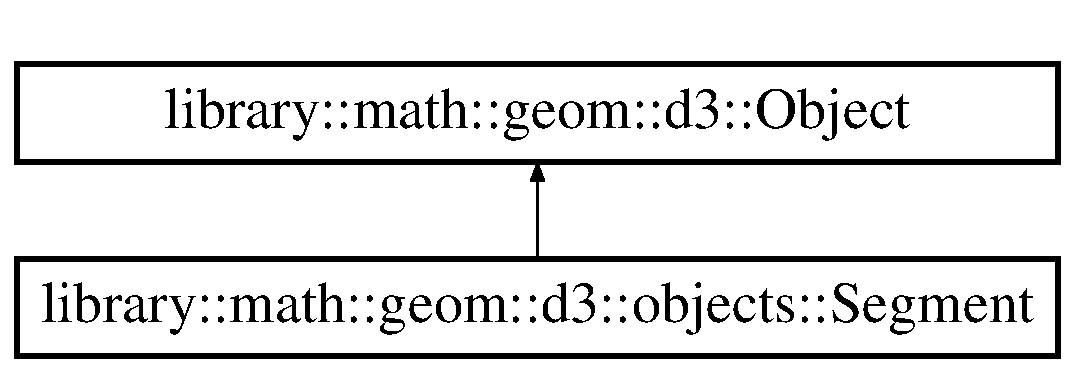
\includegraphics[height=2.000000cm]{classlibrary_1_1math_1_1geom_1_1d3_1_1objects_1_1_segment}
\end{center}
\end{figure}
\subsection*{Public Member Functions}
\begin{DoxyCompactItemize}
\item 
\hyperlink{classlibrary_1_1math_1_1geom_1_1d3_1_1objects_1_1_segment_a5562342d1edf2f52e37ce1bc138ee7d7}{Segment} (const \hyperlink{classlibrary_1_1math_1_1geom_1_1d3_1_1objects_1_1_point}{Point} \&a\+First\+Point, const \hyperlink{classlibrary_1_1math_1_1geom_1_1d3_1_1objects_1_1_point}{Point} \&a\+Second\+Point)
\begin{DoxyCompactList}\small\item\em Constructor. \end{DoxyCompactList}\item 
virtual \hyperlink{classlibrary_1_1math_1_1geom_1_1d3_1_1objects_1_1_segment}{Segment} $\ast$ \hyperlink{classlibrary_1_1math_1_1geom_1_1d3_1_1objects_1_1_segment_a589ad56339616f362cee84a2ecab61a4}{clone} () const override
\begin{DoxyCompactList}\small\item\em Clone segment. \end{DoxyCompactList}\item 
bool \hyperlink{classlibrary_1_1math_1_1geom_1_1d3_1_1objects_1_1_segment_af6b462e74438f79ec6162fdefdfcb887}{operator==} (const \hyperlink{classlibrary_1_1math_1_1geom_1_1d3_1_1objects_1_1_segment}{Segment} \&a\+Segment) const
\begin{DoxyCompactList}\small\item\em Equal to operator. \end{DoxyCompactList}\item 
bool \hyperlink{classlibrary_1_1math_1_1geom_1_1d3_1_1objects_1_1_segment_ad408a3c17a4048183c4b646ec6cf91e9}{operator!=} (const \hyperlink{classlibrary_1_1math_1_1geom_1_1d3_1_1objects_1_1_segment}{Segment} \&a\+Segment) const
\begin{DoxyCompactList}\small\item\em Not equal to operator. \end{DoxyCompactList}\item 
virtual bool \hyperlink{classlibrary_1_1math_1_1geom_1_1d3_1_1objects_1_1_segment_a70a29c3822e4859a2e8cd4a52e1b26f5}{is\+Defined} () const override
\begin{DoxyCompactList}\small\item\em Check if segment is defined. \end{DoxyCompactList}\item 
bool \hyperlink{classlibrary_1_1math_1_1geom_1_1d3_1_1objects_1_1_segment_a11324bd27db3ef9d931fdee763246759}{is\+Degenerate} () const
\begin{DoxyCompactList}\small\item\em Check if segment is degenerate, i.\+e. its length is zero. \end{DoxyCompactList}\item 
bool \hyperlink{classlibrary_1_1math_1_1geom_1_1d3_1_1objects_1_1_segment_a8ba39afb970cc57b1e11ebd5eaf82db4}{intersects} (const \hyperlink{classlibrary_1_1math_1_1geom_1_1d3_1_1objects_1_1_plane}{Plane} \&a\+Plane) const
\begin{DoxyCompactList}\small\item\em Check if segment intersects plane. \end{DoxyCompactList}\item 
bool \hyperlink{classlibrary_1_1math_1_1geom_1_1d3_1_1objects_1_1_segment_a9919183ce212b474e418685db50891fc}{intersects} (const \hyperlink{classlibrary_1_1math_1_1geom_1_1d3_1_1objects_1_1_sphere}{Sphere} \&a\+Sphere) const
\begin{DoxyCompactList}\small\item\em Check if segment intersects sphere. \end{DoxyCompactList}\item 
bool \hyperlink{classlibrary_1_1math_1_1geom_1_1d3_1_1objects_1_1_segment_af6d7eb00a6886d190c03e8b8e4220f33}{intersects} (const \hyperlink{classlibrary_1_1math_1_1geom_1_1d3_1_1objects_1_1_ellipsoid}{Ellipsoid} \&an\+Ellipsoid) const
\begin{DoxyCompactList}\small\item\em Check if segment intersects ellipsoid. \end{DoxyCompactList}\item 
bool \hyperlink{classlibrary_1_1math_1_1geom_1_1d3_1_1objects_1_1_segment_aabdbcd6bbfbe9350fe53f1b3563b5652}{contains} (const \hyperlink{classlibrary_1_1math_1_1geom_1_1d3_1_1objects_1_1_point}{Point} \&a\+Point) const
\begin{DoxyCompactList}\small\item\em Check if segment contains point. \end{DoxyCompactList}\item 
\hyperlink{classlibrary_1_1math_1_1geom_1_1d3_1_1objects_1_1_point}{Point} \hyperlink{classlibrary_1_1math_1_1geom_1_1d3_1_1objects_1_1_segment_aa51ef3e713b4041f852db4201bbf7821}{get\+First\+Point} () const
\begin{DoxyCompactList}\small\item\em Get segment first point. \end{DoxyCompactList}\item 
\hyperlink{classlibrary_1_1math_1_1geom_1_1d3_1_1objects_1_1_point}{Point} \hyperlink{classlibrary_1_1math_1_1geom_1_1d3_1_1objects_1_1_segment_a5d824fed334185975226d8f7e8489ced}{get\+Second\+Point} () const
\begin{DoxyCompactList}\small\item\em Get segment second point. \end{DoxyCompactList}\item 
\hyperlink{classlibrary_1_1math_1_1geom_1_1d3_1_1objects_1_1_point}{Point} \hyperlink{classlibrary_1_1math_1_1geom_1_1d3_1_1objects_1_1_segment_a6788da2dd6ee48ded2da197c01ea7f3d}{get\+Center} () const
\begin{DoxyCompactList}\small\item\em Get segment center. \end{DoxyCompactList}\item 
Vector3d \hyperlink{classlibrary_1_1math_1_1geom_1_1d3_1_1objects_1_1_segment_afc15a855d660d67e96467466c4442bbc}{get\+Direction} () const
\begin{DoxyCompactList}\small\item\em Get segment direction. \end{DoxyCompactList}\item 
Real \hyperlink{classlibrary_1_1math_1_1geom_1_1d3_1_1objects_1_1_segment_a16b011c680e3102b8b44e6c88ffff81d}{get\+Length} () const
\begin{DoxyCompactList}\small\item\em Get segment length. \end{DoxyCompactList}\item 
\hyperlink{classlibrary_1_1math_1_1geom_1_1d3_1_1_intersection}{Intersection} \hyperlink{classlibrary_1_1math_1_1geom_1_1d3_1_1objects_1_1_segment_a75768b02696b8ce9415b7f2da7d8f411}{intersection\+With} (const \hyperlink{classlibrary_1_1math_1_1geom_1_1d3_1_1objects_1_1_plane}{Plane} \&a\+Plane) const
\begin{DoxyCompactList}\small\item\em Compute intersection of segment with plane. \end{DoxyCompactList}\item 
virtual void \hyperlink{classlibrary_1_1math_1_1geom_1_1d3_1_1objects_1_1_segment_a2d3c1a17842ee4ee83cffda33911291d}{print} (std\+::ostream \&an\+Output\+Stream, bool display\+Decorators=true) const override
\begin{DoxyCompactList}\small\item\em Print segment. \end{DoxyCompactList}\item 
virtual void \hyperlink{classlibrary_1_1math_1_1geom_1_1d3_1_1objects_1_1_segment_a63c7017391bcc0e67f4d97311e7ebdb2}{apply\+Transformation} (const \hyperlink{classlibrary_1_1math_1_1geom_1_1d3_1_1_transformation}{Transformation} \&a\+Transformation) override
\begin{DoxyCompactList}\small\item\em Apply transformation to segment. \end{DoxyCompactList}\end{DoxyCompactItemize}
\subsection*{Static Public Member Functions}
\begin{DoxyCompactItemize}
\item 
static \hyperlink{classlibrary_1_1math_1_1geom_1_1d3_1_1objects_1_1_segment}{Segment} \hyperlink{classlibrary_1_1math_1_1geom_1_1d3_1_1objects_1_1_segment_a3b2505e9553ba0067f8184120c106602}{Undefined} ()
\begin{DoxyCompactList}\small\item\em Constructs an undefined segment. \end{DoxyCompactList}\end{DoxyCompactItemize}


\subsection{Detailed Description}
\hyperlink{classlibrary_1_1math_1_1geom_1_1d3_1_1objects_1_1_segment}{Segment}. 

A segment is a part of a line that is bounded by two distinct end points, and contains every point on the line between its endpoints.

https\+://en.wikipedia.\+org/wiki/\+Line\+\_\+segment 

\subsection{Constructor \& Destructor Documentation}
\mbox{\Hypertarget{classlibrary_1_1math_1_1geom_1_1d3_1_1objects_1_1_segment_a5562342d1edf2f52e37ce1bc138ee7d7}\label{classlibrary_1_1math_1_1geom_1_1d3_1_1objects_1_1_segment_a5562342d1edf2f52e37ce1bc138ee7d7}} 
\index{library\+::math\+::geom\+::d3\+::objects\+::\+Segment@{library\+::math\+::geom\+::d3\+::objects\+::\+Segment}!Segment@{Segment}}
\index{Segment@{Segment}!library\+::math\+::geom\+::d3\+::objects\+::\+Segment@{library\+::math\+::geom\+::d3\+::objects\+::\+Segment}}
\subsubsection{\texorpdfstring{Segment()}{Segment()}}
{\footnotesize\ttfamily library\+::math\+::geom\+::d3\+::objects\+::\+Segment\+::\+Segment (\begin{DoxyParamCaption}\item[{const \hyperlink{classlibrary_1_1math_1_1geom_1_1d3_1_1objects_1_1_point}{Point} \&}]{a\+First\+Point,  }\item[{const \hyperlink{classlibrary_1_1math_1_1geom_1_1d3_1_1objects_1_1_point}{Point} \&}]{a\+Second\+Point }\end{DoxyParamCaption})}



Constructor. 


\begin{DoxyCode}
\hyperlink{classlibrary_1_1math_1_1geom_1_1d3_1_1objects_1_1_segment_a5562342d1edf2f52e37ce1bc138ee7d7}{Segment} segment(\{ 0.0, 0.0, 0.0 \}, \{ 0.0, 0.0, 1.0 \}) ;
\end{DoxyCode}



\begin{DoxyParams}[1]{Parameters}
\mbox{\tt in}  & {\em a\+First\+Point} & A first point \\
\hline
\mbox{\tt in}  & {\em a\+Second\+Point} & A second point \\
\hline
\end{DoxyParams}


\subsection{Member Function Documentation}
\mbox{\Hypertarget{classlibrary_1_1math_1_1geom_1_1d3_1_1objects_1_1_segment_a63c7017391bcc0e67f4d97311e7ebdb2}\label{classlibrary_1_1math_1_1geom_1_1d3_1_1objects_1_1_segment_a63c7017391bcc0e67f4d97311e7ebdb2}} 
\index{library\+::math\+::geom\+::d3\+::objects\+::\+Segment@{library\+::math\+::geom\+::d3\+::objects\+::\+Segment}!apply\+Transformation@{apply\+Transformation}}
\index{apply\+Transformation@{apply\+Transformation}!library\+::math\+::geom\+::d3\+::objects\+::\+Segment@{library\+::math\+::geom\+::d3\+::objects\+::\+Segment}}
\subsubsection{\texorpdfstring{apply\+Transformation()}{applyTransformation()}}
{\footnotesize\ttfamily void library\+::math\+::geom\+::d3\+::objects\+::\+Segment\+::apply\+Transformation (\begin{DoxyParamCaption}\item[{const \hyperlink{classlibrary_1_1math_1_1geom_1_1d3_1_1_transformation}{Transformation} \&}]{a\+Transformation }\end{DoxyParamCaption})\hspace{0.3cm}{\ttfamily [override]}, {\ttfamily [virtual]}}



Apply transformation to segment. 


\begin{DoxyParams}[1]{Parameters}
\mbox{\tt in}  & {\em a\+Transformation} & A transformation \\
\hline
\end{DoxyParams}


Implements \hyperlink{classlibrary_1_1math_1_1geom_1_1d3_1_1_object_a5fc47b1ee5d9a28efc6010d3d1512470}{library\+::math\+::geom\+::d3\+::\+Object}.

\mbox{\Hypertarget{classlibrary_1_1math_1_1geom_1_1d3_1_1objects_1_1_segment_a589ad56339616f362cee84a2ecab61a4}\label{classlibrary_1_1math_1_1geom_1_1d3_1_1objects_1_1_segment_a589ad56339616f362cee84a2ecab61a4}} 
\index{library\+::math\+::geom\+::d3\+::objects\+::\+Segment@{library\+::math\+::geom\+::d3\+::objects\+::\+Segment}!clone@{clone}}
\index{clone@{clone}!library\+::math\+::geom\+::d3\+::objects\+::\+Segment@{library\+::math\+::geom\+::d3\+::objects\+::\+Segment}}
\subsubsection{\texorpdfstring{clone()}{clone()}}
{\footnotesize\ttfamily \hyperlink{classlibrary_1_1math_1_1geom_1_1d3_1_1objects_1_1_segment}{Segment} $\ast$ library\+::math\+::geom\+::d3\+::objects\+::\+Segment\+::clone (\begin{DoxyParamCaption}{ }\end{DoxyParamCaption}) const\hspace{0.3cm}{\ttfamily [override]}, {\ttfamily [virtual]}}



Clone segment. 

\begin{DoxyReturn}{Returns}
Pointer to cloned segment 
\end{DoxyReturn}


Implements \hyperlink{classlibrary_1_1math_1_1geom_1_1d3_1_1_object_a1a784c6b359e0eb97cd34fabc42f2f3f}{library\+::math\+::geom\+::d3\+::\+Object}.

\mbox{\Hypertarget{classlibrary_1_1math_1_1geom_1_1d3_1_1objects_1_1_segment_aabdbcd6bbfbe9350fe53f1b3563b5652}\label{classlibrary_1_1math_1_1geom_1_1d3_1_1objects_1_1_segment_aabdbcd6bbfbe9350fe53f1b3563b5652}} 
\index{library\+::math\+::geom\+::d3\+::objects\+::\+Segment@{library\+::math\+::geom\+::d3\+::objects\+::\+Segment}!contains@{contains}}
\index{contains@{contains}!library\+::math\+::geom\+::d3\+::objects\+::\+Segment@{library\+::math\+::geom\+::d3\+::objects\+::\+Segment}}
\subsubsection{\texorpdfstring{contains()}{contains()}}
{\footnotesize\ttfamily bool library\+::math\+::geom\+::d3\+::objects\+::\+Segment\+::contains (\begin{DoxyParamCaption}\item[{const \hyperlink{classlibrary_1_1math_1_1geom_1_1d3_1_1objects_1_1_point}{Point} \&}]{a\+Point }\end{DoxyParamCaption}) const}



Check if segment contains point. 


\begin{DoxyCode}
\hyperlink{classlibrary_1_1math_1_1geom_1_1d3_1_1objects_1_1_segment_a5562342d1edf2f52e37ce1bc138ee7d7}{Segment} segment = ... ;
Point point = ... ;
segment.contains(point) ;
\end{DoxyCode}



\begin{DoxyParams}[1]{Parameters}
\mbox{\tt in}  & {\em a\+Point} & A point \\
\hline
\end{DoxyParams}
\begin{DoxyReturn}{Returns}
True if segment contains point 
\end{DoxyReturn}
\mbox{\Hypertarget{classlibrary_1_1math_1_1geom_1_1d3_1_1objects_1_1_segment_a6788da2dd6ee48ded2da197c01ea7f3d}\label{classlibrary_1_1math_1_1geom_1_1d3_1_1objects_1_1_segment_a6788da2dd6ee48ded2da197c01ea7f3d}} 
\index{library\+::math\+::geom\+::d3\+::objects\+::\+Segment@{library\+::math\+::geom\+::d3\+::objects\+::\+Segment}!get\+Center@{get\+Center}}
\index{get\+Center@{get\+Center}!library\+::math\+::geom\+::d3\+::objects\+::\+Segment@{library\+::math\+::geom\+::d3\+::objects\+::\+Segment}}
\subsubsection{\texorpdfstring{get\+Center()}{getCenter()}}
{\footnotesize\ttfamily \hyperlink{classlibrary_1_1math_1_1geom_1_1d3_1_1objects_1_1_point}{Point} library\+::math\+::geom\+::d3\+::objects\+::\+Segment\+::get\+Center (\begin{DoxyParamCaption}{ }\end{DoxyParamCaption}) const}



Get segment center. 


\begin{DoxyCode}
\hyperlink{classlibrary_1_1math_1_1geom_1_1d3_1_1objects_1_1_segment_a5562342d1edf2f52e37ce1bc138ee7d7}{Segment}(\{ 0.0, 0.0, 0.0 \}, \{ 0.0, 0.0, 2.0 \}).\hyperlink{classlibrary_1_1math_1_1geom_1_1d3_1_1objects_1_1_segment_a6788da2dd6ee48ded2da197c01ea7f3d}{getCenter}() ; \textcolor{comment}{// [0.0, 0.0, 1.0]}
\end{DoxyCode}


\begin{DoxyReturn}{Returns}
\hyperlink{classlibrary_1_1math_1_1geom_1_1d3_1_1objects_1_1_segment}{Segment} center 
\end{DoxyReturn}
\mbox{\Hypertarget{classlibrary_1_1math_1_1geom_1_1d3_1_1objects_1_1_segment_afc15a855d660d67e96467466c4442bbc}\label{classlibrary_1_1math_1_1geom_1_1d3_1_1objects_1_1_segment_afc15a855d660d67e96467466c4442bbc}} 
\index{library\+::math\+::geom\+::d3\+::objects\+::\+Segment@{library\+::math\+::geom\+::d3\+::objects\+::\+Segment}!get\+Direction@{get\+Direction}}
\index{get\+Direction@{get\+Direction}!library\+::math\+::geom\+::d3\+::objects\+::\+Segment@{library\+::math\+::geom\+::d3\+::objects\+::\+Segment}}
\subsubsection{\texorpdfstring{get\+Direction()}{getDirection()}}
{\footnotesize\ttfamily Vector3d library\+::math\+::geom\+::d3\+::objects\+::\+Segment\+::get\+Direction (\begin{DoxyParamCaption}{ }\end{DoxyParamCaption}) const}



Get segment direction. 


\begin{DoxyCode}
\hyperlink{classlibrary_1_1math_1_1geom_1_1d3_1_1objects_1_1_segment_a5562342d1edf2f52e37ce1bc138ee7d7}{Segment}(\{ 0.0, 0.0, 0.0 \}, \{ 0.0, 0.0, 2.0 \}).\hyperlink{classlibrary_1_1math_1_1geom_1_1d3_1_1objects_1_1_segment_afc15a855d660d67e96467466c4442bbc}{getDirection}() ; \textcolor{comment}{// [0.0, 0.0, 1.0]}
\end{DoxyCode}


\begin{DoxyReturn}{Returns}
\hyperlink{classlibrary_1_1math_1_1geom_1_1d3_1_1objects_1_1_segment}{Segment} direction 
\end{DoxyReturn}
\mbox{\Hypertarget{classlibrary_1_1math_1_1geom_1_1d3_1_1objects_1_1_segment_aa51ef3e713b4041f852db4201bbf7821}\label{classlibrary_1_1math_1_1geom_1_1d3_1_1objects_1_1_segment_aa51ef3e713b4041f852db4201bbf7821}} 
\index{library\+::math\+::geom\+::d3\+::objects\+::\+Segment@{library\+::math\+::geom\+::d3\+::objects\+::\+Segment}!get\+First\+Point@{get\+First\+Point}}
\index{get\+First\+Point@{get\+First\+Point}!library\+::math\+::geom\+::d3\+::objects\+::\+Segment@{library\+::math\+::geom\+::d3\+::objects\+::\+Segment}}
\subsubsection{\texorpdfstring{get\+First\+Point()}{getFirstPoint()}}
{\footnotesize\ttfamily \hyperlink{classlibrary_1_1math_1_1geom_1_1d3_1_1objects_1_1_point}{Point} library\+::math\+::geom\+::d3\+::objects\+::\+Segment\+::get\+First\+Point (\begin{DoxyParamCaption}{ }\end{DoxyParamCaption}) const}



Get segment first point. 


\begin{DoxyCode}
\hyperlink{classlibrary_1_1math_1_1geom_1_1d3_1_1objects_1_1_segment_a5562342d1edf2f52e37ce1bc138ee7d7}{Segment}(\{ 0.0, 0.0, 0.0 \}, \{ 0.0, 0.0, 1.0 \}).\hyperlink{classlibrary_1_1math_1_1geom_1_1d3_1_1objects_1_1_segment_aa51ef3e713b4041f852db4201bbf7821}{getFirstPoint}() ; \textcolor{comment}{// [0.0, 0.0, 0.0]}
\end{DoxyCode}


\begin{DoxyReturn}{Returns}
\hyperlink{classlibrary_1_1math_1_1geom_1_1d3_1_1objects_1_1_segment}{Segment} first point 
\end{DoxyReturn}
\mbox{\Hypertarget{classlibrary_1_1math_1_1geom_1_1d3_1_1objects_1_1_segment_a16b011c680e3102b8b44e6c88ffff81d}\label{classlibrary_1_1math_1_1geom_1_1d3_1_1objects_1_1_segment_a16b011c680e3102b8b44e6c88ffff81d}} 
\index{library\+::math\+::geom\+::d3\+::objects\+::\+Segment@{library\+::math\+::geom\+::d3\+::objects\+::\+Segment}!get\+Length@{get\+Length}}
\index{get\+Length@{get\+Length}!library\+::math\+::geom\+::d3\+::objects\+::\+Segment@{library\+::math\+::geom\+::d3\+::objects\+::\+Segment}}
\subsubsection{\texorpdfstring{get\+Length()}{getLength()}}
{\footnotesize\ttfamily Real library\+::math\+::geom\+::d3\+::objects\+::\+Segment\+::get\+Length (\begin{DoxyParamCaption}{ }\end{DoxyParamCaption}) const}



Get segment length. 


\begin{DoxyCode}
\hyperlink{classlibrary_1_1math_1_1geom_1_1d3_1_1objects_1_1_segment_a5562342d1edf2f52e37ce1bc138ee7d7}{Segment}(\{ 0.0, 0.0, 0.0 \}, \{ 0.0, 0.0, 2.0 \}).\hyperlink{classlibrary_1_1math_1_1geom_1_1d3_1_1objects_1_1_segment_a16b011c680e3102b8b44e6c88ffff81d}{getLength}() ; \textcolor{comment}{// 2.0}
\end{DoxyCode}


\begin{DoxyReturn}{Returns}
\hyperlink{classlibrary_1_1math_1_1geom_1_1d3_1_1objects_1_1_segment}{Segment} length 
\end{DoxyReturn}
\mbox{\Hypertarget{classlibrary_1_1math_1_1geom_1_1d3_1_1objects_1_1_segment_a5d824fed334185975226d8f7e8489ced}\label{classlibrary_1_1math_1_1geom_1_1d3_1_1objects_1_1_segment_a5d824fed334185975226d8f7e8489ced}} 
\index{library\+::math\+::geom\+::d3\+::objects\+::\+Segment@{library\+::math\+::geom\+::d3\+::objects\+::\+Segment}!get\+Second\+Point@{get\+Second\+Point}}
\index{get\+Second\+Point@{get\+Second\+Point}!library\+::math\+::geom\+::d3\+::objects\+::\+Segment@{library\+::math\+::geom\+::d3\+::objects\+::\+Segment}}
\subsubsection{\texorpdfstring{get\+Second\+Point()}{getSecondPoint()}}
{\footnotesize\ttfamily \hyperlink{classlibrary_1_1math_1_1geom_1_1d3_1_1objects_1_1_point}{Point} library\+::math\+::geom\+::d3\+::objects\+::\+Segment\+::get\+Second\+Point (\begin{DoxyParamCaption}{ }\end{DoxyParamCaption}) const}



Get segment second point. 


\begin{DoxyCode}
\hyperlink{classlibrary_1_1math_1_1geom_1_1d3_1_1objects_1_1_segment_a5562342d1edf2f52e37ce1bc138ee7d7}{Segment}(\{ 0.0, 0.0, 0.0 \}, \{ 0.0, 0.0, 1.0 \}).\hyperlink{classlibrary_1_1math_1_1geom_1_1d3_1_1objects_1_1_segment_a5d824fed334185975226d8f7e8489ced}{getSecondPoint}() ; \textcolor{comment}{// [0.0, 0.0, 1.0]}
\end{DoxyCode}


\begin{DoxyReturn}{Returns}
\hyperlink{classlibrary_1_1math_1_1geom_1_1d3_1_1objects_1_1_segment}{Segment} second point 
\end{DoxyReturn}
\mbox{\Hypertarget{classlibrary_1_1math_1_1geom_1_1d3_1_1objects_1_1_segment_a75768b02696b8ce9415b7f2da7d8f411}\label{classlibrary_1_1math_1_1geom_1_1d3_1_1objects_1_1_segment_a75768b02696b8ce9415b7f2da7d8f411}} 
\index{library\+::math\+::geom\+::d3\+::objects\+::\+Segment@{library\+::math\+::geom\+::d3\+::objects\+::\+Segment}!intersection\+With@{intersection\+With}}
\index{intersection\+With@{intersection\+With}!library\+::math\+::geom\+::d3\+::objects\+::\+Segment@{library\+::math\+::geom\+::d3\+::objects\+::\+Segment}}
\subsubsection{\texorpdfstring{intersection\+With()}{intersectionWith()}}
{\footnotesize\ttfamily \hyperlink{classlibrary_1_1math_1_1geom_1_1d3_1_1_intersection}{Intersection} library\+::math\+::geom\+::d3\+::objects\+::\+Segment\+::intersection\+With (\begin{DoxyParamCaption}\item[{const \hyperlink{classlibrary_1_1math_1_1geom_1_1d3_1_1objects_1_1_plane}{Plane} \&}]{a\+Plane }\end{DoxyParamCaption}) const}



Compute intersection of segment with plane. 


\begin{DoxyParams}[1]{Parameters}
\mbox{\tt in}  & {\em a\+Plane} & A plane \\
\hline
\end{DoxyParams}
\begin{DoxyReturn}{Returns}
\hyperlink{classlibrary_1_1math_1_1geom_1_1d3_1_1_intersection}{Intersection} of segment with plane 
\end{DoxyReturn}
\mbox{\Hypertarget{classlibrary_1_1math_1_1geom_1_1d3_1_1objects_1_1_segment_a8ba39afb970cc57b1e11ebd5eaf82db4}\label{classlibrary_1_1math_1_1geom_1_1d3_1_1objects_1_1_segment_a8ba39afb970cc57b1e11ebd5eaf82db4}} 
\index{library\+::math\+::geom\+::d3\+::objects\+::\+Segment@{library\+::math\+::geom\+::d3\+::objects\+::\+Segment}!intersects@{intersects}}
\index{intersects@{intersects}!library\+::math\+::geom\+::d3\+::objects\+::\+Segment@{library\+::math\+::geom\+::d3\+::objects\+::\+Segment}}
\subsubsection{\texorpdfstring{intersects()}{intersects()}\hspace{0.1cm}{\footnotesize\ttfamily [1/3]}}
{\footnotesize\ttfamily bool library\+::math\+::geom\+::d3\+::objects\+::\+Segment\+::intersects (\begin{DoxyParamCaption}\item[{const \hyperlink{classlibrary_1_1math_1_1geom_1_1d3_1_1objects_1_1_plane}{Plane} \&}]{a\+Plane }\end{DoxyParamCaption}) const}



Check if segment intersects plane. 


\begin{DoxyCode}
\hyperlink{classlibrary_1_1math_1_1geom_1_1d3_1_1objects_1_1_segment_a5562342d1edf2f52e37ce1bc138ee7d7}{Segment} segment = ... ;
Plane plane = ... ;
segment.intersects(plane) ;
\end{DoxyCode}



\begin{DoxyParams}[1]{Parameters}
\mbox{\tt in}  & {\em a\+Plane} & A plane \\
\hline
\end{DoxyParams}
\begin{DoxyReturn}{Returns}
True if segment intersects plane 
\end{DoxyReturn}
\mbox{\Hypertarget{classlibrary_1_1math_1_1geom_1_1d3_1_1objects_1_1_segment_a9919183ce212b474e418685db50891fc}\label{classlibrary_1_1math_1_1geom_1_1d3_1_1objects_1_1_segment_a9919183ce212b474e418685db50891fc}} 
\index{library\+::math\+::geom\+::d3\+::objects\+::\+Segment@{library\+::math\+::geom\+::d3\+::objects\+::\+Segment}!intersects@{intersects}}
\index{intersects@{intersects}!library\+::math\+::geom\+::d3\+::objects\+::\+Segment@{library\+::math\+::geom\+::d3\+::objects\+::\+Segment}}
\subsubsection{\texorpdfstring{intersects()}{intersects()}\hspace{0.1cm}{\footnotesize\ttfamily [2/3]}}
{\footnotesize\ttfamily bool library\+::math\+::geom\+::d3\+::objects\+::\+Segment\+::intersects (\begin{DoxyParamCaption}\item[{const \hyperlink{classlibrary_1_1math_1_1geom_1_1d3_1_1objects_1_1_sphere}{Sphere} \&}]{a\+Sphere }\end{DoxyParamCaption}) const}



Check if segment intersects sphere. 


\begin{DoxyCode}
\hyperlink{classlibrary_1_1math_1_1geom_1_1d3_1_1objects_1_1_segment_a5562342d1edf2f52e37ce1bc138ee7d7}{Segment} segment = ... ;
Sphere sphere = ... ;
segment.intersects(sphere) ;
\end{DoxyCode}



\begin{DoxyParams}[1]{Parameters}
\mbox{\tt in}  & {\em a\+Sphere} & A sphere \\
\hline
\end{DoxyParams}
\begin{DoxyReturn}{Returns}
True if segment intersects sphere 
\end{DoxyReturn}
\mbox{\Hypertarget{classlibrary_1_1math_1_1geom_1_1d3_1_1objects_1_1_segment_af6d7eb00a6886d190c03e8b8e4220f33}\label{classlibrary_1_1math_1_1geom_1_1d3_1_1objects_1_1_segment_af6d7eb00a6886d190c03e8b8e4220f33}} 
\index{library\+::math\+::geom\+::d3\+::objects\+::\+Segment@{library\+::math\+::geom\+::d3\+::objects\+::\+Segment}!intersects@{intersects}}
\index{intersects@{intersects}!library\+::math\+::geom\+::d3\+::objects\+::\+Segment@{library\+::math\+::geom\+::d3\+::objects\+::\+Segment}}
\subsubsection{\texorpdfstring{intersects()}{intersects()}\hspace{0.1cm}{\footnotesize\ttfamily [3/3]}}
{\footnotesize\ttfamily bool library\+::math\+::geom\+::d3\+::objects\+::\+Segment\+::intersects (\begin{DoxyParamCaption}\item[{const \hyperlink{classlibrary_1_1math_1_1geom_1_1d3_1_1objects_1_1_ellipsoid}{Ellipsoid} \&}]{an\+Ellipsoid }\end{DoxyParamCaption}) const}



Check if segment intersects ellipsoid. 


\begin{DoxyCode}
\hyperlink{classlibrary_1_1math_1_1geom_1_1d3_1_1objects_1_1_segment_a5562342d1edf2f52e37ce1bc138ee7d7}{Segment} segment = ... ;
Ellipsoid ellipsoid = ... ;
segment.intersects(ellipsoid) ;
\end{DoxyCode}



\begin{DoxyParams}[1]{Parameters}
\mbox{\tt in}  & {\em an\+Ellipsoid} & An ellipsoid \\
\hline
\end{DoxyParams}
\begin{DoxyReturn}{Returns}
True if segment intersects ellipsoid 
\end{DoxyReturn}
\mbox{\Hypertarget{classlibrary_1_1math_1_1geom_1_1d3_1_1objects_1_1_segment_a70a29c3822e4859a2e8cd4a52e1b26f5}\label{classlibrary_1_1math_1_1geom_1_1d3_1_1objects_1_1_segment_a70a29c3822e4859a2e8cd4a52e1b26f5}} 
\index{library\+::math\+::geom\+::d3\+::objects\+::\+Segment@{library\+::math\+::geom\+::d3\+::objects\+::\+Segment}!is\+Defined@{is\+Defined}}
\index{is\+Defined@{is\+Defined}!library\+::math\+::geom\+::d3\+::objects\+::\+Segment@{library\+::math\+::geom\+::d3\+::objects\+::\+Segment}}
\subsubsection{\texorpdfstring{is\+Defined()}{isDefined()}}
{\footnotesize\ttfamily bool library\+::math\+::geom\+::d3\+::objects\+::\+Segment\+::is\+Defined (\begin{DoxyParamCaption}{ }\end{DoxyParamCaption}) const\hspace{0.3cm}{\ttfamily [override]}, {\ttfamily [virtual]}}



Check if segment is defined. 


\begin{DoxyCode}
\hyperlink{classlibrary_1_1math_1_1geom_1_1d3_1_1objects_1_1_segment_a5562342d1edf2f52e37ce1bc138ee7d7}{Segment}(\{ 0.0, 0.0, 0.0 \}, \{ 0.0, 0.0, 1.0 \}).\hyperlink{classlibrary_1_1math_1_1geom_1_1d3_1_1objects_1_1_segment_a70a29c3822e4859a2e8cd4a52e1b26f5}{isDefined}() ; \textcolor{comment}{// True}
\end{DoxyCode}


\begin{DoxyReturn}{Returns}
True if segment is defined 
\end{DoxyReturn}


Implements \hyperlink{classlibrary_1_1math_1_1geom_1_1d3_1_1_object_a2216442e322f0c3ca5f01a4efa22baf7}{library\+::math\+::geom\+::d3\+::\+Object}.

\mbox{\Hypertarget{classlibrary_1_1math_1_1geom_1_1d3_1_1objects_1_1_segment_a11324bd27db3ef9d931fdee763246759}\label{classlibrary_1_1math_1_1geom_1_1d3_1_1objects_1_1_segment_a11324bd27db3ef9d931fdee763246759}} 
\index{library\+::math\+::geom\+::d3\+::objects\+::\+Segment@{library\+::math\+::geom\+::d3\+::objects\+::\+Segment}!is\+Degenerate@{is\+Degenerate}}
\index{is\+Degenerate@{is\+Degenerate}!library\+::math\+::geom\+::d3\+::objects\+::\+Segment@{library\+::math\+::geom\+::d3\+::objects\+::\+Segment}}
\subsubsection{\texorpdfstring{is\+Degenerate()}{isDegenerate()}}
{\footnotesize\ttfamily bool library\+::math\+::geom\+::d3\+::objects\+::\+Segment\+::is\+Degenerate (\begin{DoxyParamCaption}{ }\end{DoxyParamCaption}) const}



Check if segment is degenerate, i.\+e. its length is zero. 


\begin{DoxyCode}
\hyperlink{classlibrary_1_1math_1_1geom_1_1d3_1_1objects_1_1_segment_a5562342d1edf2f52e37ce1bc138ee7d7}{Segment}(\{ 0.0, 0.0, 0.0 \}, \{ 0.0, 0.0, 0.0 \}).\hyperlink{classlibrary_1_1math_1_1geom_1_1d3_1_1objects_1_1_segment_a11324bd27db3ef9d931fdee763246759}{isDegenerate}() ; \textcolor{comment}{// True}
\end{DoxyCode}


\begin{DoxyReturn}{Returns}
True if segment is degenerate 
\end{DoxyReturn}
\mbox{\Hypertarget{classlibrary_1_1math_1_1geom_1_1d3_1_1objects_1_1_segment_ad408a3c17a4048183c4b646ec6cf91e9}\label{classlibrary_1_1math_1_1geom_1_1d3_1_1objects_1_1_segment_ad408a3c17a4048183c4b646ec6cf91e9}} 
\index{library\+::math\+::geom\+::d3\+::objects\+::\+Segment@{library\+::math\+::geom\+::d3\+::objects\+::\+Segment}!operator"!=@{operator"!=}}
\index{operator"!=@{operator"!=}!library\+::math\+::geom\+::d3\+::objects\+::\+Segment@{library\+::math\+::geom\+::d3\+::objects\+::\+Segment}}
\subsubsection{\texorpdfstring{operator"!=()}{operator!=()}}
{\footnotesize\ttfamily bool library\+::math\+::geom\+::d3\+::objects\+::\+Segment\+::operator!= (\begin{DoxyParamCaption}\item[{const \hyperlink{classlibrary_1_1math_1_1geom_1_1d3_1_1objects_1_1_segment}{Segment} \&}]{a\+Segment }\end{DoxyParamCaption}) const}



Not equal to operator. 


\begin{DoxyCode}
\hyperlink{classlibrary_1_1math_1_1geom_1_1d3_1_1objects_1_1_segment_a5562342d1edf2f52e37ce1bc138ee7d7}{Segment}(\{ 0.0, 0.0, 0.0 \}, \{ 0.0, 0.0, 1.0 \}) != \hyperlink{classlibrary_1_1math_1_1geom_1_1d3_1_1objects_1_1_segment_a5562342d1edf2f52e37ce1bc138ee7d7}{Segment}(\{ 0.0, 0.0, 0.0 \}, \{ 0.0, 0.0, 2.0 \}
      ) ; \textcolor{comment}{// True}
\end{DoxyCode}



\begin{DoxyParams}[1]{Parameters}
\mbox{\tt in}  & {\em a\+Segment} & A segment \\
\hline
\end{DoxyParams}
\begin{DoxyReturn}{Returns}
True if segments are not equal 
\end{DoxyReturn}
\mbox{\Hypertarget{classlibrary_1_1math_1_1geom_1_1d3_1_1objects_1_1_segment_af6b462e74438f79ec6162fdefdfcb887}\label{classlibrary_1_1math_1_1geom_1_1d3_1_1objects_1_1_segment_af6b462e74438f79ec6162fdefdfcb887}} 
\index{library\+::math\+::geom\+::d3\+::objects\+::\+Segment@{library\+::math\+::geom\+::d3\+::objects\+::\+Segment}!operator==@{operator==}}
\index{operator==@{operator==}!library\+::math\+::geom\+::d3\+::objects\+::\+Segment@{library\+::math\+::geom\+::d3\+::objects\+::\+Segment}}
\subsubsection{\texorpdfstring{operator==()}{operator==()}}
{\footnotesize\ttfamily bool library\+::math\+::geom\+::d3\+::objects\+::\+Segment\+::operator== (\begin{DoxyParamCaption}\item[{const \hyperlink{classlibrary_1_1math_1_1geom_1_1d3_1_1objects_1_1_segment}{Segment} \&}]{a\+Segment }\end{DoxyParamCaption}) const}



Equal to operator. 


\begin{DoxyCode}
\hyperlink{classlibrary_1_1math_1_1geom_1_1d3_1_1objects_1_1_segment_a5562342d1edf2f52e37ce1bc138ee7d7}{Segment}(\{ 0.0, 0.0, 0.0 \}, \{ 0.0, 0.0, 1.0 \}) == \hyperlink{classlibrary_1_1math_1_1geom_1_1d3_1_1objects_1_1_segment_a5562342d1edf2f52e37ce1bc138ee7d7}{Segment}(\{ 0.0, 0.0, 0.0 \}, \{ 0.0, 0.0, 1.0 \}
      ) ; \textcolor{comment}{// True}
\end{DoxyCode}



\begin{DoxyParams}[1]{Parameters}
\mbox{\tt in}  & {\em a\+Segment} & A segment \\
\hline
\end{DoxyParams}
\begin{DoxyReturn}{Returns}
True if segments are equal 
\end{DoxyReturn}
\mbox{\Hypertarget{classlibrary_1_1math_1_1geom_1_1d3_1_1objects_1_1_segment_a2d3c1a17842ee4ee83cffda33911291d}\label{classlibrary_1_1math_1_1geom_1_1d3_1_1objects_1_1_segment_a2d3c1a17842ee4ee83cffda33911291d}} 
\index{library\+::math\+::geom\+::d3\+::objects\+::\+Segment@{library\+::math\+::geom\+::d3\+::objects\+::\+Segment}!print@{print}}
\index{print@{print}!library\+::math\+::geom\+::d3\+::objects\+::\+Segment@{library\+::math\+::geom\+::d3\+::objects\+::\+Segment}}
\subsubsection{\texorpdfstring{print()}{print()}}
{\footnotesize\ttfamily void library\+::math\+::geom\+::d3\+::objects\+::\+Segment\+::print (\begin{DoxyParamCaption}\item[{std\+::ostream \&}]{an\+Output\+Stream,  }\item[{bool}]{display\+Decorators = {\ttfamily true} }\end{DoxyParamCaption}) const\hspace{0.3cm}{\ttfamily [override]}, {\ttfamily [virtual]}}



Print segment. 


\begin{DoxyParams}[1]{Parameters}
\mbox{\tt in}  & {\em an\+Output\+Stream} & An output stream \\
\hline
\mbox{\tt in}  & {\em (optional)} & display\+Decorators If true, display decorators \\
\hline
\end{DoxyParams}


Implements \hyperlink{classlibrary_1_1math_1_1geom_1_1d3_1_1_object_aa166f4ce4d116a248f0fc861c75012ca}{library\+::math\+::geom\+::d3\+::\+Object}.

\mbox{\Hypertarget{classlibrary_1_1math_1_1geom_1_1d3_1_1objects_1_1_segment_a3b2505e9553ba0067f8184120c106602}\label{classlibrary_1_1math_1_1geom_1_1d3_1_1objects_1_1_segment_a3b2505e9553ba0067f8184120c106602}} 
\index{library\+::math\+::geom\+::d3\+::objects\+::\+Segment@{library\+::math\+::geom\+::d3\+::objects\+::\+Segment}!Undefined@{Undefined}}
\index{Undefined@{Undefined}!library\+::math\+::geom\+::d3\+::objects\+::\+Segment@{library\+::math\+::geom\+::d3\+::objects\+::\+Segment}}
\subsubsection{\texorpdfstring{Undefined()}{Undefined()}}
{\footnotesize\ttfamily \hyperlink{classlibrary_1_1math_1_1geom_1_1d3_1_1objects_1_1_segment}{Segment} library\+::math\+::geom\+::d3\+::objects\+::\+Segment\+::\+Undefined (\begin{DoxyParamCaption}{ }\end{DoxyParamCaption})\hspace{0.3cm}{\ttfamily [static]}}



Constructs an undefined segment. 


\begin{DoxyCode}
\hyperlink{classlibrary_1_1math_1_1geom_1_1d3_1_1objects_1_1_segment_a5562342d1edf2f52e37ce1bc138ee7d7}{Segment} segment = \hyperlink{classlibrary_1_1math_1_1geom_1_1d3_1_1objects_1_1_segment_a3b2505e9553ba0067f8184120c106602}{Segment::Undefined}() ; \textcolor{comment}{// Undefined}
\end{DoxyCode}


\begin{DoxyReturn}{Returns}
Undefined segment 
\end{DoxyReturn}


The documentation for this class was generated from the following files\+:\begin{DoxyCompactItemize}
\item 
include/\+Library/\+Mathematics/\+Geometry/3\+D/\+Objects/\hyperlink{3_d_2_objects_2_segment_8hpp}{Segment.\+hpp}\item 
src/\+Library/\+Mathematics/\+Geometry/3\+D/\+Objects/\hyperlink{3_d_2_objects_2_segment_8cpp}{Segment.\+cpp}\end{DoxyCompactItemize}

\hypertarget{classlibrary_1_1math_1_1geom_1_1d2_1_1objects_1_1_segment}{}\section{library\+:\+:math\+:\+:geom\+:\+:d2\+:\+:objects\+:\+:Segment Class Reference}
\label{classlibrary_1_1math_1_1geom_1_1d2_1_1objects_1_1_segment}\index{library\+::math\+::geom\+::d2\+::objects\+::\+Segment@{library\+::math\+::geom\+::d2\+::objects\+::\+Segment}}


\hyperlink{classlibrary_1_1math_1_1geom_1_1d2_1_1objects_1_1_segment}{Segment}.  




{\ttfamily \#include $<$Segment.\+hpp$>$}

Inheritance diagram for library\+:\+:math\+:\+:geom\+:\+:d2\+:\+:objects\+:\+:Segment\+:\begin{figure}[H]
\begin{center}
\leavevmode
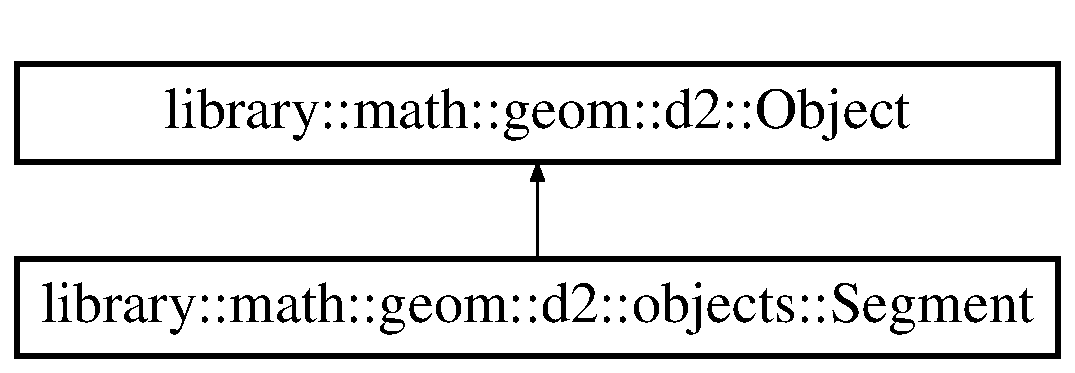
\includegraphics[height=2.000000cm]{classlibrary_1_1math_1_1geom_1_1d2_1_1objects_1_1_segment}
\end{center}
\end{figure}
\subsection*{Public Member Functions}
\begin{DoxyCompactItemize}
\item 
\hyperlink{classlibrary_1_1math_1_1geom_1_1d2_1_1objects_1_1_segment_a44ba44fd5f02a02fe34c40223b38fa8f}{Segment} (const \hyperlink{classlibrary_1_1math_1_1geom_1_1d2_1_1objects_1_1_point}{Point} \&a\+First\+Point, const \hyperlink{classlibrary_1_1math_1_1geom_1_1d2_1_1objects_1_1_point}{Point} \&a\+Second\+Point)
\begin{DoxyCompactList}\small\item\em Constructor. \end{DoxyCompactList}\item 
virtual \hyperlink{classlibrary_1_1math_1_1geom_1_1d2_1_1objects_1_1_segment}{Segment} $\ast$ \hyperlink{classlibrary_1_1math_1_1geom_1_1d2_1_1objects_1_1_segment_a6149a3cf215b0b573d5bd4f25fad75e9}{clone} () const override
\begin{DoxyCompactList}\small\item\em Clone segment. \end{DoxyCompactList}\item 
bool \hyperlink{classlibrary_1_1math_1_1geom_1_1d2_1_1objects_1_1_segment_a639981918aaa52807452451b19dbf680}{operator==} (const \hyperlink{classlibrary_1_1math_1_1geom_1_1d2_1_1objects_1_1_segment}{Segment} \&a\+Segment) const
\begin{DoxyCompactList}\small\item\em Equal to operator. \end{DoxyCompactList}\item 
bool \hyperlink{classlibrary_1_1math_1_1geom_1_1d2_1_1objects_1_1_segment_ad7a06e9fc322b3baaf4c5ecf3a22d559}{operator!=} (const \hyperlink{classlibrary_1_1math_1_1geom_1_1d2_1_1objects_1_1_segment}{Segment} \&a\+Segment) const
\begin{DoxyCompactList}\small\item\em Not equal to operator. \end{DoxyCompactList}\item 
virtual bool \hyperlink{classlibrary_1_1math_1_1geom_1_1d2_1_1objects_1_1_segment_a2c366d74328cdce4a7e83a761a84dbc7}{is\+Defined} () const override
\begin{DoxyCompactList}\small\item\em Check if segment is defined. \end{DoxyCompactList}\item 
bool \hyperlink{classlibrary_1_1math_1_1geom_1_1d2_1_1objects_1_1_segment_a0ed58e12b0d91a83fdea0c13308a3d37}{is\+Degenerate} () const
\begin{DoxyCompactList}\small\item\em Check if segment is degenerate, i.\+e. its length is zero. \end{DoxyCompactList}\item 
bool \hyperlink{classlibrary_1_1math_1_1geom_1_1d2_1_1objects_1_1_segment_ac72deb794d609e44ccddf1cde25a7c2d}{contains} (const \hyperlink{classlibrary_1_1math_1_1geom_1_1d2_1_1objects_1_1_point}{Point} \&a\+Point) const
\begin{DoxyCompactList}\small\item\em Check if segment contains point. \end{DoxyCompactList}\item 
bool \hyperlink{classlibrary_1_1math_1_1geom_1_1d2_1_1objects_1_1_segment_a501ffbc0492c4b9e279bba7b7a79ae89}{contains} (const \hyperlink{classlibrary_1_1math_1_1geom_1_1d2_1_1objects_1_1_point_set}{Point\+Set} \&a\+Point\+Set) const
\begin{DoxyCompactList}\small\item\em Check if segment contains point set. \end{DoxyCompactList}\item 
\hyperlink{classlibrary_1_1math_1_1geom_1_1d2_1_1objects_1_1_point}{Point} \hyperlink{classlibrary_1_1math_1_1geom_1_1d2_1_1objects_1_1_segment_aa78aa20d97d8d9cb23737260e7e308b5}{get\+First\+Point} () const
\begin{DoxyCompactList}\small\item\em Get segment first point. \end{DoxyCompactList}\item 
\hyperlink{classlibrary_1_1math_1_1geom_1_1d2_1_1objects_1_1_point}{Point} \hyperlink{classlibrary_1_1math_1_1geom_1_1d2_1_1objects_1_1_segment_acf79cfdb28dec7d497382a3ea650491c}{get\+Second\+Point} () const
\begin{DoxyCompactList}\small\item\em Get segment second point. \end{DoxyCompactList}\item 
\hyperlink{classlibrary_1_1math_1_1geom_1_1d2_1_1objects_1_1_point}{Point} \hyperlink{classlibrary_1_1math_1_1geom_1_1d2_1_1objects_1_1_segment_a964684b33e11314a0b818fb089a197e6}{get\+Center} () const
\begin{DoxyCompactList}\small\item\em Get segment center. \end{DoxyCompactList}\item 
Vector2d \hyperlink{classlibrary_1_1math_1_1geom_1_1d2_1_1objects_1_1_segment_af7b2a7dbc7be4941740699a93c63a690}{get\+Direction} () const
\begin{DoxyCompactList}\small\item\em Get segment direction. \end{DoxyCompactList}\item 
Real \hyperlink{classlibrary_1_1math_1_1geom_1_1d2_1_1objects_1_1_segment_a19ed354dd888d7581f14a8217c2af4a5}{get\+Length} () const
\begin{DoxyCompactList}\small\item\em Get segment length. \end{DoxyCompactList}\item 
virtual String \hyperlink{classlibrary_1_1math_1_1geom_1_1d2_1_1objects_1_1_segment_a6efb82e3e5e5d97214b827bc6f8574e3}{to\+String} (const \hyperlink{classlibrary_1_1math_1_1geom_1_1d2_1_1_object_ac8cd61dada4960cfee9a469231621b17}{Object\+::\+Format} \&a\+Format=\hyperlink{classlibrary_1_1math_1_1geom_1_1d2_1_1_object_ac8cd61dada4960cfee9a469231621b17aeb6d8ae6f20283755b339c0dc273988b}{Object\+::\+Format\+::\+Standard}, const Integer \&a\+Precision=Integer\+::\+Undefined()) const override
\begin{DoxyCompactList}\small\item\em Get string representation. \end{DoxyCompactList}\item 
virtual void \hyperlink{classlibrary_1_1math_1_1geom_1_1d2_1_1objects_1_1_segment_abfe0b4983dcb9e26848d29a9b86d4b9c}{print} (std\+::ostream \&an\+Output\+Stream, bool display\+Decorators=true) const override
\begin{DoxyCompactList}\small\item\em Print segment. \end{DoxyCompactList}\item 
virtual void \hyperlink{classlibrary_1_1math_1_1geom_1_1d2_1_1objects_1_1_segment_a5cb71beeb4de3c2c1b84fbfb8546c935}{apply\+Transformation} (const \hyperlink{classlibrary_1_1math_1_1geom_1_1d2_1_1_transformation}{Transformation} \&a\+Transformation) override
\begin{DoxyCompactList}\small\item\em Apply transformation to segment. \end{DoxyCompactList}\end{DoxyCompactItemize}
\subsection*{Static Public Member Functions}
\begin{DoxyCompactItemize}
\item 
static \hyperlink{classlibrary_1_1math_1_1geom_1_1d2_1_1objects_1_1_segment}{Segment} \hyperlink{classlibrary_1_1math_1_1geom_1_1d2_1_1objects_1_1_segment_a8df8fa90e8294482a88fec4eb4c449f5}{Undefined} ()
\begin{DoxyCompactList}\small\item\em Constructs an undefined segment. \end{DoxyCompactList}\end{DoxyCompactItemize}
\subsection*{Additional Inherited Members}


\subsection{Detailed Description}
\hyperlink{classlibrary_1_1math_1_1geom_1_1d2_1_1objects_1_1_segment}{Segment}. 

A segment is a part of a line that is bounded by two distinct end points, and contains every point on the line between its endpoints.

https\+://en.wikipedia.\+org/wiki/\+Line\+\_\+segment 

\subsection{Constructor \& Destructor Documentation}
\mbox{\Hypertarget{classlibrary_1_1math_1_1geom_1_1d2_1_1objects_1_1_segment_a44ba44fd5f02a02fe34c40223b38fa8f}\label{classlibrary_1_1math_1_1geom_1_1d2_1_1objects_1_1_segment_a44ba44fd5f02a02fe34c40223b38fa8f}} 
\index{library\+::math\+::geom\+::d2\+::objects\+::\+Segment@{library\+::math\+::geom\+::d2\+::objects\+::\+Segment}!Segment@{Segment}}
\index{Segment@{Segment}!library\+::math\+::geom\+::d2\+::objects\+::\+Segment@{library\+::math\+::geom\+::d2\+::objects\+::\+Segment}}
\subsubsection{\texorpdfstring{Segment()}{Segment()}}
{\footnotesize\ttfamily library\+::math\+::geom\+::d2\+::objects\+::\+Segment\+::\+Segment (\begin{DoxyParamCaption}\item[{const \hyperlink{classlibrary_1_1math_1_1geom_1_1d2_1_1objects_1_1_point}{Point} \&}]{a\+First\+Point,  }\item[{const \hyperlink{classlibrary_1_1math_1_1geom_1_1d2_1_1objects_1_1_point}{Point} \&}]{a\+Second\+Point }\end{DoxyParamCaption})}



Constructor. 


\begin{DoxyCode}
\hyperlink{classlibrary_1_1math_1_1geom_1_1d2_1_1objects_1_1_segment_a44ba44fd5f02a02fe34c40223b38fa8f}{Segment} segment(\{ 0.0, 0.0 \}, \{ 0.0, 1.0 \}) ;
\end{DoxyCode}



\begin{DoxyParams}[1]{Parameters}
\mbox{\tt in}  & {\em a\+First\+Point} & A first point \\
\hline
\mbox{\tt in}  & {\em a\+Second\+Point} & A second point \\
\hline
\end{DoxyParams}


\subsection{Member Function Documentation}
\mbox{\Hypertarget{classlibrary_1_1math_1_1geom_1_1d2_1_1objects_1_1_segment_a5cb71beeb4de3c2c1b84fbfb8546c935}\label{classlibrary_1_1math_1_1geom_1_1d2_1_1objects_1_1_segment_a5cb71beeb4de3c2c1b84fbfb8546c935}} 
\index{library\+::math\+::geom\+::d2\+::objects\+::\+Segment@{library\+::math\+::geom\+::d2\+::objects\+::\+Segment}!apply\+Transformation@{apply\+Transformation}}
\index{apply\+Transformation@{apply\+Transformation}!library\+::math\+::geom\+::d2\+::objects\+::\+Segment@{library\+::math\+::geom\+::d2\+::objects\+::\+Segment}}
\subsubsection{\texorpdfstring{apply\+Transformation()}{applyTransformation()}}
{\footnotesize\ttfamily void library\+::math\+::geom\+::d2\+::objects\+::\+Segment\+::apply\+Transformation (\begin{DoxyParamCaption}\item[{const \hyperlink{classlibrary_1_1math_1_1geom_1_1d2_1_1_transformation}{Transformation} \&}]{a\+Transformation }\end{DoxyParamCaption})\hspace{0.3cm}{\ttfamily [override]}, {\ttfamily [virtual]}}



Apply transformation to segment. 


\begin{DoxyParams}[1]{Parameters}
\mbox{\tt in}  & {\em a\+Transformation} & A transformation \\
\hline
\end{DoxyParams}


Implements \hyperlink{classlibrary_1_1math_1_1geom_1_1d2_1_1_object_a289589fb6e9e7a2c4ca4976a1544def5}{library\+::math\+::geom\+::d2\+::\+Object}.

\mbox{\Hypertarget{classlibrary_1_1math_1_1geom_1_1d2_1_1objects_1_1_segment_a6149a3cf215b0b573d5bd4f25fad75e9}\label{classlibrary_1_1math_1_1geom_1_1d2_1_1objects_1_1_segment_a6149a3cf215b0b573d5bd4f25fad75e9}} 
\index{library\+::math\+::geom\+::d2\+::objects\+::\+Segment@{library\+::math\+::geom\+::d2\+::objects\+::\+Segment}!clone@{clone}}
\index{clone@{clone}!library\+::math\+::geom\+::d2\+::objects\+::\+Segment@{library\+::math\+::geom\+::d2\+::objects\+::\+Segment}}
\subsubsection{\texorpdfstring{clone()}{clone()}}
{\footnotesize\ttfamily \hyperlink{classlibrary_1_1math_1_1geom_1_1d2_1_1objects_1_1_segment}{Segment} $\ast$ library\+::math\+::geom\+::d2\+::objects\+::\+Segment\+::clone (\begin{DoxyParamCaption}{ }\end{DoxyParamCaption}) const\hspace{0.3cm}{\ttfamily [override]}, {\ttfamily [virtual]}}



Clone segment. 

\begin{DoxyReturn}{Returns}
Pointer to cloned segment 
\end{DoxyReturn}


Implements \hyperlink{classlibrary_1_1math_1_1geom_1_1d2_1_1_object_a5c26ae4120edb24f6463d65a9cef247d}{library\+::math\+::geom\+::d2\+::\+Object}.

\mbox{\Hypertarget{classlibrary_1_1math_1_1geom_1_1d2_1_1objects_1_1_segment_ac72deb794d609e44ccddf1cde25a7c2d}\label{classlibrary_1_1math_1_1geom_1_1d2_1_1objects_1_1_segment_ac72deb794d609e44ccddf1cde25a7c2d}} 
\index{library\+::math\+::geom\+::d2\+::objects\+::\+Segment@{library\+::math\+::geom\+::d2\+::objects\+::\+Segment}!contains@{contains}}
\index{contains@{contains}!library\+::math\+::geom\+::d2\+::objects\+::\+Segment@{library\+::math\+::geom\+::d2\+::objects\+::\+Segment}}
\subsubsection{\texorpdfstring{contains()}{contains()}\hspace{0.1cm}{\footnotesize\ttfamily [1/2]}}
{\footnotesize\ttfamily bool library\+::math\+::geom\+::d2\+::objects\+::\+Segment\+::contains (\begin{DoxyParamCaption}\item[{const \hyperlink{classlibrary_1_1math_1_1geom_1_1d2_1_1objects_1_1_point}{Point} \&}]{a\+Point }\end{DoxyParamCaption}) const}



Check if segment contains point. 


\begin{DoxyCode}
\hyperlink{classlibrary_1_1math_1_1geom_1_1d2_1_1objects_1_1_segment_a44ba44fd5f02a02fe34c40223b38fa8f}{Segment} segment = ... ;
Point point = ... ;
segment.contains(point) ;
\end{DoxyCode}



\begin{DoxyParams}[1]{Parameters}
\mbox{\tt in}  & {\em a\+Point} & A point \\
\hline
\end{DoxyParams}
\begin{DoxyReturn}{Returns}
True if segment contains point 
\end{DoxyReturn}
\mbox{\Hypertarget{classlibrary_1_1math_1_1geom_1_1d2_1_1objects_1_1_segment_a501ffbc0492c4b9e279bba7b7a79ae89}\label{classlibrary_1_1math_1_1geom_1_1d2_1_1objects_1_1_segment_a501ffbc0492c4b9e279bba7b7a79ae89}} 
\index{library\+::math\+::geom\+::d2\+::objects\+::\+Segment@{library\+::math\+::geom\+::d2\+::objects\+::\+Segment}!contains@{contains}}
\index{contains@{contains}!library\+::math\+::geom\+::d2\+::objects\+::\+Segment@{library\+::math\+::geom\+::d2\+::objects\+::\+Segment}}
\subsubsection{\texorpdfstring{contains()}{contains()}\hspace{0.1cm}{\footnotesize\ttfamily [2/2]}}
{\footnotesize\ttfamily bool library\+::math\+::geom\+::d2\+::objects\+::\+Segment\+::contains (\begin{DoxyParamCaption}\item[{const \hyperlink{classlibrary_1_1math_1_1geom_1_1d2_1_1objects_1_1_point_set}{Point\+Set} \&}]{a\+Point\+Set }\end{DoxyParamCaption}) const}



Check if segment contains point set. 


\begin{DoxyCode}
\hyperlink{classlibrary_1_1math_1_1geom_1_1d2_1_1objects_1_1_segment_a44ba44fd5f02a02fe34c40223b38fa8f}{Segment} segment = ... ;
PointSet pointSet = ... ;
segment.contains(pointSet) ;
\end{DoxyCode}



\begin{DoxyParams}[1]{Parameters}
\mbox{\tt in}  & {\em a\+Point\+Set} & A point set \\
\hline
\end{DoxyParams}
\begin{DoxyReturn}{Returns}
True if segment contains point set 
\end{DoxyReturn}
\mbox{\Hypertarget{classlibrary_1_1math_1_1geom_1_1d2_1_1objects_1_1_segment_a964684b33e11314a0b818fb089a197e6}\label{classlibrary_1_1math_1_1geom_1_1d2_1_1objects_1_1_segment_a964684b33e11314a0b818fb089a197e6}} 
\index{library\+::math\+::geom\+::d2\+::objects\+::\+Segment@{library\+::math\+::geom\+::d2\+::objects\+::\+Segment}!get\+Center@{get\+Center}}
\index{get\+Center@{get\+Center}!library\+::math\+::geom\+::d2\+::objects\+::\+Segment@{library\+::math\+::geom\+::d2\+::objects\+::\+Segment}}
\subsubsection{\texorpdfstring{get\+Center()}{getCenter()}}
{\footnotesize\ttfamily \hyperlink{classlibrary_1_1math_1_1geom_1_1d2_1_1objects_1_1_point}{Point} library\+::math\+::geom\+::d2\+::objects\+::\+Segment\+::get\+Center (\begin{DoxyParamCaption}{ }\end{DoxyParamCaption}) const}



Get segment center. 


\begin{DoxyCode}
\hyperlink{classlibrary_1_1math_1_1geom_1_1d2_1_1objects_1_1_segment_a44ba44fd5f02a02fe34c40223b38fa8f}{Segment}(\{ 0.0, 0.0 \}, \{ 0.0, 2.0 \}).\hyperlink{classlibrary_1_1math_1_1geom_1_1d2_1_1objects_1_1_segment_a964684b33e11314a0b818fb089a197e6}{getCenter}() ; \textcolor{comment}{// [0.0, 1.0]}
\end{DoxyCode}


\begin{DoxyReturn}{Returns}
\hyperlink{classlibrary_1_1math_1_1geom_1_1d2_1_1objects_1_1_segment}{Segment} center 
\end{DoxyReturn}
\mbox{\Hypertarget{classlibrary_1_1math_1_1geom_1_1d2_1_1objects_1_1_segment_af7b2a7dbc7be4941740699a93c63a690}\label{classlibrary_1_1math_1_1geom_1_1d2_1_1objects_1_1_segment_af7b2a7dbc7be4941740699a93c63a690}} 
\index{library\+::math\+::geom\+::d2\+::objects\+::\+Segment@{library\+::math\+::geom\+::d2\+::objects\+::\+Segment}!get\+Direction@{get\+Direction}}
\index{get\+Direction@{get\+Direction}!library\+::math\+::geom\+::d2\+::objects\+::\+Segment@{library\+::math\+::geom\+::d2\+::objects\+::\+Segment}}
\subsubsection{\texorpdfstring{get\+Direction()}{getDirection()}}
{\footnotesize\ttfamily Vector2d library\+::math\+::geom\+::d2\+::objects\+::\+Segment\+::get\+Direction (\begin{DoxyParamCaption}{ }\end{DoxyParamCaption}) const}



Get segment direction. 


\begin{DoxyCode}
\hyperlink{classlibrary_1_1math_1_1geom_1_1d2_1_1objects_1_1_segment_a44ba44fd5f02a02fe34c40223b38fa8f}{Segment}(\{ 0.0, 0.0 \}, \{ 0.0, 2.0 \}).\hyperlink{classlibrary_1_1math_1_1geom_1_1d2_1_1objects_1_1_segment_af7b2a7dbc7be4941740699a93c63a690}{getDirection}() ; \textcolor{comment}{// [0.0, 1.0]}
\end{DoxyCode}


\begin{DoxyReturn}{Returns}
\hyperlink{classlibrary_1_1math_1_1geom_1_1d2_1_1objects_1_1_segment}{Segment} direction 
\end{DoxyReturn}
\mbox{\Hypertarget{classlibrary_1_1math_1_1geom_1_1d2_1_1objects_1_1_segment_aa78aa20d97d8d9cb23737260e7e308b5}\label{classlibrary_1_1math_1_1geom_1_1d2_1_1objects_1_1_segment_aa78aa20d97d8d9cb23737260e7e308b5}} 
\index{library\+::math\+::geom\+::d2\+::objects\+::\+Segment@{library\+::math\+::geom\+::d2\+::objects\+::\+Segment}!get\+First\+Point@{get\+First\+Point}}
\index{get\+First\+Point@{get\+First\+Point}!library\+::math\+::geom\+::d2\+::objects\+::\+Segment@{library\+::math\+::geom\+::d2\+::objects\+::\+Segment}}
\subsubsection{\texorpdfstring{get\+First\+Point()}{getFirstPoint()}}
{\footnotesize\ttfamily \hyperlink{classlibrary_1_1math_1_1geom_1_1d2_1_1objects_1_1_point}{Point} library\+::math\+::geom\+::d2\+::objects\+::\+Segment\+::get\+First\+Point (\begin{DoxyParamCaption}{ }\end{DoxyParamCaption}) const}



Get segment first point. 


\begin{DoxyCode}
\hyperlink{classlibrary_1_1math_1_1geom_1_1d2_1_1objects_1_1_segment_a44ba44fd5f02a02fe34c40223b38fa8f}{Segment}(\{ 0.0, 0.0 \}, \{ 0.0, 1.0 \}).\hyperlink{classlibrary_1_1math_1_1geom_1_1d2_1_1objects_1_1_segment_aa78aa20d97d8d9cb23737260e7e308b5}{getFirstPoint}() ; \textcolor{comment}{// [0.0, 0.0]}
\end{DoxyCode}


\begin{DoxyReturn}{Returns}
\hyperlink{classlibrary_1_1math_1_1geom_1_1d2_1_1objects_1_1_segment}{Segment} first point 
\end{DoxyReturn}
\mbox{\Hypertarget{classlibrary_1_1math_1_1geom_1_1d2_1_1objects_1_1_segment_a19ed354dd888d7581f14a8217c2af4a5}\label{classlibrary_1_1math_1_1geom_1_1d2_1_1objects_1_1_segment_a19ed354dd888d7581f14a8217c2af4a5}} 
\index{library\+::math\+::geom\+::d2\+::objects\+::\+Segment@{library\+::math\+::geom\+::d2\+::objects\+::\+Segment}!get\+Length@{get\+Length}}
\index{get\+Length@{get\+Length}!library\+::math\+::geom\+::d2\+::objects\+::\+Segment@{library\+::math\+::geom\+::d2\+::objects\+::\+Segment}}
\subsubsection{\texorpdfstring{get\+Length()}{getLength()}}
{\footnotesize\ttfamily Real library\+::math\+::geom\+::d2\+::objects\+::\+Segment\+::get\+Length (\begin{DoxyParamCaption}{ }\end{DoxyParamCaption}) const}



Get segment length. 


\begin{DoxyCode}
\hyperlink{classlibrary_1_1math_1_1geom_1_1d2_1_1objects_1_1_segment_a44ba44fd5f02a02fe34c40223b38fa8f}{Segment}(\{ 0.0, 0.0 \}, \{ 0.0, 2.0 \}).\hyperlink{classlibrary_1_1math_1_1geom_1_1d2_1_1objects_1_1_segment_a19ed354dd888d7581f14a8217c2af4a5}{getLength}() ; \textcolor{comment}{// 2.0}
\end{DoxyCode}


\begin{DoxyReturn}{Returns}
\hyperlink{classlibrary_1_1math_1_1geom_1_1d2_1_1objects_1_1_segment}{Segment} length 
\end{DoxyReturn}
\mbox{\Hypertarget{classlibrary_1_1math_1_1geom_1_1d2_1_1objects_1_1_segment_acf79cfdb28dec7d497382a3ea650491c}\label{classlibrary_1_1math_1_1geom_1_1d2_1_1objects_1_1_segment_acf79cfdb28dec7d497382a3ea650491c}} 
\index{library\+::math\+::geom\+::d2\+::objects\+::\+Segment@{library\+::math\+::geom\+::d2\+::objects\+::\+Segment}!get\+Second\+Point@{get\+Second\+Point}}
\index{get\+Second\+Point@{get\+Second\+Point}!library\+::math\+::geom\+::d2\+::objects\+::\+Segment@{library\+::math\+::geom\+::d2\+::objects\+::\+Segment}}
\subsubsection{\texorpdfstring{get\+Second\+Point()}{getSecondPoint()}}
{\footnotesize\ttfamily \hyperlink{classlibrary_1_1math_1_1geom_1_1d2_1_1objects_1_1_point}{Point} library\+::math\+::geom\+::d2\+::objects\+::\+Segment\+::get\+Second\+Point (\begin{DoxyParamCaption}{ }\end{DoxyParamCaption}) const}



Get segment second point. 


\begin{DoxyCode}
\hyperlink{classlibrary_1_1math_1_1geom_1_1d2_1_1objects_1_1_segment_a44ba44fd5f02a02fe34c40223b38fa8f}{Segment}(\{ 0.0, 0.0 \}, \{ 0.0, 1.0 \}).\hyperlink{classlibrary_1_1math_1_1geom_1_1d2_1_1objects_1_1_segment_acf79cfdb28dec7d497382a3ea650491c}{getSecondPoint}() ; \textcolor{comment}{// [0.0, 1.0]}
\end{DoxyCode}


\begin{DoxyReturn}{Returns}
\hyperlink{classlibrary_1_1math_1_1geom_1_1d2_1_1objects_1_1_segment}{Segment} second point 
\end{DoxyReturn}
\mbox{\Hypertarget{classlibrary_1_1math_1_1geom_1_1d2_1_1objects_1_1_segment_a2c366d74328cdce4a7e83a761a84dbc7}\label{classlibrary_1_1math_1_1geom_1_1d2_1_1objects_1_1_segment_a2c366d74328cdce4a7e83a761a84dbc7}} 
\index{library\+::math\+::geom\+::d2\+::objects\+::\+Segment@{library\+::math\+::geom\+::d2\+::objects\+::\+Segment}!is\+Defined@{is\+Defined}}
\index{is\+Defined@{is\+Defined}!library\+::math\+::geom\+::d2\+::objects\+::\+Segment@{library\+::math\+::geom\+::d2\+::objects\+::\+Segment}}
\subsubsection{\texorpdfstring{is\+Defined()}{isDefined()}}
{\footnotesize\ttfamily bool library\+::math\+::geom\+::d2\+::objects\+::\+Segment\+::is\+Defined (\begin{DoxyParamCaption}{ }\end{DoxyParamCaption}) const\hspace{0.3cm}{\ttfamily [override]}, {\ttfamily [virtual]}}



Check if segment is defined. 


\begin{DoxyCode}
\hyperlink{classlibrary_1_1math_1_1geom_1_1d2_1_1objects_1_1_segment_a44ba44fd5f02a02fe34c40223b38fa8f}{Segment}(\{ 0.0, 0.0 \}, \{ 0.0, 1.0 \}).\hyperlink{classlibrary_1_1math_1_1geom_1_1d2_1_1objects_1_1_segment_a2c366d74328cdce4a7e83a761a84dbc7}{isDefined}() ; \textcolor{comment}{// True}
\end{DoxyCode}


\begin{DoxyReturn}{Returns}
True if segment is defined 
\end{DoxyReturn}


Implements \hyperlink{classlibrary_1_1math_1_1geom_1_1d2_1_1_object_ae9506254971168a3ca63e1923556b70d}{library\+::math\+::geom\+::d2\+::\+Object}.

\mbox{\Hypertarget{classlibrary_1_1math_1_1geom_1_1d2_1_1objects_1_1_segment_a0ed58e12b0d91a83fdea0c13308a3d37}\label{classlibrary_1_1math_1_1geom_1_1d2_1_1objects_1_1_segment_a0ed58e12b0d91a83fdea0c13308a3d37}} 
\index{library\+::math\+::geom\+::d2\+::objects\+::\+Segment@{library\+::math\+::geom\+::d2\+::objects\+::\+Segment}!is\+Degenerate@{is\+Degenerate}}
\index{is\+Degenerate@{is\+Degenerate}!library\+::math\+::geom\+::d2\+::objects\+::\+Segment@{library\+::math\+::geom\+::d2\+::objects\+::\+Segment}}
\subsubsection{\texorpdfstring{is\+Degenerate()}{isDegenerate()}}
{\footnotesize\ttfamily bool library\+::math\+::geom\+::d2\+::objects\+::\+Segment\+::is\+Degenerate (\begin{DoxyParamCaption}{ }\end{DoxyParamCaption}) const}



Check if segment is degenerate, i.\+e. its length is zero. 


\begin{DoxyCode}
\hyperlink{classlibrary_1_1math_1_1geom_1_1d2_1_1objects_1_1_segment_a44ba44fd5f02a02fe34c40223b38fa8f}{Segment}(\{ 0.0, 0.0 \}, \{ 0.0, 0.0 \}).\hyperlink{classlibrary_1_1math_1_1geom_1_1d2_1_1objects_1_1_segment_a0ed58e12b0d91a83fdea0c13308a3d37}{isDegenerate}() ; \textcolor{comment}{// True}
\end{DoxyCode}


\begin{DoxyReturn}{Returns}
True if segment is degenerate 
\end{DoxyReturn}
\mbox{\Hypertarget{classlibrary_1_1math_1_1geom_1_1d2_1_1objects_1_1_segment_ad7a06e9fc322b3baaf4c5ecf3a22d559}\label{classlibrary_1_1math_1_1geom_1_1d2_1_1objects_1_1_segment_ad7a06e9fc322b3baaf4c5ecf3a22d559}} 
\index{library\+::math\+::geom\+::d2\+::objects\+::\+Segment@{library\+::math\+::geom\+::d2\+::objects\+::\+Segment}!operator"!=@{operator"!=}}
\index{operator"!=@{operator"!=}!library\+::math\+::geom\+::d2\+::objects\+::\+Segment@{library\+::math\+::geom\+::d2\+::objects\+::\+Segment}}
\subsubsection{\texorpdfstring{operator"!=()}{operator!=()}}
{\footnotesize\ttfamily bool library\+::math\+::geom\+::d2\+::objects\+::\+Segment\+::operator!= (\begin{DoxyParamCaption}\item[{const \hyperlink{classlibrary_1_1math_1_1geom_1_1d2_1_1objects_1_1_segment}{Segment} \&}]{a\+Segment }\end{DoxyParamCaption}) const}



Not equal to operator. 


\begin{DoxyCode}
\hyperlink{classlibrary_1_1math_1_1geom_1_1d2_1_1objects_1_1_segment_a44ba44fd5f02a02fe34c40223b38fa8f}{Segment}(\{ 0.0, 0.0 \}, \{ 0.0, 1.0 \}) != \hyperlink{classlibrary_1_1math_1_1geom_1_1d2_1_1objects_1_1_segment_a44ba44fd5f02a02fe34c40223b38fa8f}{Segment}(\{ 0.0, 0.0 \}, \{ 0.0, 2.0 \}) ; \textcolor{comment}{// True}
\end{DoxyCode}



\begin{DoxyParams}[1]{Parameters}
\mbox{\tt in}  & {\em a\+Segment} & A segment \\
\hline
\end{DoxyParams}
\begin{DoxyReturn}{Returns}
True if segments are not equal 
\end{DoxyReturn}
\mbox{\Hypertarget{classlibrary_1_1math_1_1geom_1_1d2_1_1objects_1_1_segment_a639981918aaa52807452451b19dbf680}\label{classlibrary_1_1math_1_1geom_1_1d2_1_1objects_1_1_segment_a639981918aaa52807452451b19dbf680}} 
\index{library\+::math\+::geom\+::d2\+::objects\+::\+Segment@{library\+::math\+::geom\+::d2\+::objects\+::\+Segment}!operator==@{operator==}}
\index{operator==@{operator==}!library\+::math\+::geom\+::d2\+::objects\+::\+Segment@{library\+::math\+::geom\+::d2\+::objects\+::\+Segment}}
\subsubsection{\texorpdfstring{operator==()}{operator==()}}
{\footnotesize\ttfamily bool library\+::math\+::geom\+::d2\+::objects\+::\+Segment\+::operator== (\begin{DoxyParamCaption}\item[{const \hyperlink{classlibrary_1_1math_1_1geom_1_1d2_1_1objects_1_1_segment}{Segment} \&}]{a\+Segment }\end{DoxyParamCaption}) const}



Equal to operator. 


\begin{DoxyCode}
\hyperlink{classlibrary_1_1math_1_1geom_1_1d2_1_1objects_1_1_segment_a44ba44fd5f02a02fe34c40223b38fa8f}{Segment}(\{ 0.0, 0.0 \}, \{ 0.0, 1.0 \}) == \hyperlink{classlibrary_1_1math_1_1geom_1_1d2_1_1objects_1_1_segment_a44ba44fd5f02a02fe34c40223b38fa8f}{Segment}(\{ 0.0, 0.0 \}, \{ 0.0, 1.0 \}) ; \textcolor{comment}{// True}
\end{DoxyCode}



\begin{DoxyParams}[1]{Parameters}
\mbox{\tt in}  & {\em a\+Segment} & A segment \\
\hline
\end{DoxyParams}
\begin{DoxyReturn}{Returns}
True if segments are equal 
\end{DoxyReturn}
\mbox{\Hypertarget{classlibrary_1_1math_1_1geom_1_1d2_1_1objects_1_1_segment_abfe0b4983dcb9e26848d29a9b86d4b9c}\label{classlibrary_1_1math_1_1geom_1_1d2_1_1objects_1_1_segment_abfe0b4983dcb9e26848d29a9b86d4b9c}} 
\index{library\+::math\+::geom\+::d2\+::objects\+::\+Segment@{library\+::math\+::geom\+::d2\+::objects\+::\+Segment}!print@{print}}
\index{print@{print}!library\+::math\+::geom\+::d2\+::objects\+::\+Segment@{library\+::math\+::geom\+::d2\+::objects\+::\+Segment}}
\subsubsection{\texorpdfstring{print()}{print()}}
{\footnotesize\ttfamily void library\+::math\+::geom\+::d2\+::objects\+::\+Segment\+::print (\begin{DoxyParamCaption}\item[{std\+::ostream \&}]{an\+Output\+Stream,  }\item[{bool}]{display\+Decorators = {\ttfamily true} }\end{DoxyParamCaption}) const\hspace{0.3cm}{\ttfamily [override]}, {\ttfamily [virtual]}}



Print segment. 


\begin{DoxyParams}[1]{Parameters}
\mbox{\tt in}  & {\em an\+Output\+Stream} & An output stream \\
\hline
\mbox{\tt in}  & {\em (optional)} & display\+Decorators If true, display decorators \\
\hline
\end{DoxyParams}


Implements \hyperlink{classlibrary_1_1math_1_1geom_1_1d2_1_1_object_a834bbf59cf1c483d1dc7b0966b1e1ab3}{library\+::math\+::geom\+::d2\+::\+Object}.

\mbox{\Hypertarget{classlibrary_1_1math_1_1geom_1_1d2_1_1objects_1_1_segment_a6efb82e3e5e5d97214b827bc6f8574e3}\label{classlibrary_1_1math_1_1geom_1_1d2_1_1objects_1_1_segment_a6efb82e3e5e5d97214b827bc6f8574e3}} 
\index{library\+::math\+::geom\+::d2\+::objects\+::\+Segment@{library\+::math\+::geom\+::d2\+::objects\+::\+Segment}!to\+String@{to\+String}}
\index{to\+String@{to\+String}!library\+::math\+::geom\+::d2\+::objects\+::\+Segment@{library\+::math\+::geom\+::d2\+::objects\+::\+Segment}}
\subsubsection{\texorpdfstring{to\+String()}{toString()}}
{\footnotesize\ttfamily String library\+::math\+::geom\+::d2\+::objects\+::\+Segment\+::to\+String (\begin{DoxyParamCaption}\item[{const \hyperlink{classlibrary_1_1math_1_1geom_1_1d2_1_1_object_ac8cd61dada4960cfee9a469231621b17}{Object\+::\+Format} \&}]{a\+Format = {\ttfamily \hyperlink{classlibrary_1_1math_1_1geom_1_1d2_1_1_object_ac8cd61dada4960cfee9a469231621b17aeb6d8ae6f20283755b339c0dc273988b}{Object\+::\+Format\+::\+Standard}},  }\item[{const Integer \&}]{a\+Precision = {\ttfamily Integer\+:\+:Undefined()} }\end{DoxyParamCaption}) const\hspace{0.3cm}{\ttfamily [override]}, {\ttfamily [virtual]}}



Get string representation. 


\begin{DoxyParams}[1]{Parameters}
\mbox{\tt in}  & {\em a\+Format} & A format \\
\hline
\end{DoxyParams}
\begin{DoxyReturn}{Returns}
String representation 
\end{DoxyReturn}


Implements \hyperlink{classlibrary_1_1math_1_1geom_1_1d2_1_1_object_acdd76b3637732a249536b609dbe3f0eb}{library\+::math\+::geom\+::d2\+::\+Object}.

\mbox{\Hypertarget{classlibrary_1_1math_1_1geom_1_1d2_1_1objects_1_1_segment_a8df8fa90e8294482a88fec4eb4c449f5}\label{classlibrary_1_1math_1_1geom_1_1d2_1_1objects_1_1_segment_a8df8fa90e8294482a88fec4eb4c449f5}} 
\index{library\+::math\+::geom\+::d2\+::objects\+::\+Segment@{library\+::math\+::geom\+::d2\+::objects\+::\+Segment}!Undefined@{Undefined}}
\index{Undefined@{Undefined}!library\+::math\+::geom\+::d2\+::objects\+::\+Segment@{library\+::math\+::geom\+::d2\+::objects\+::\+Segment}}
\subsubsection{\texorpdfstring{Undefined()}{Undefined()}}
{\footnotesize\ttfamily \hyperlink{classlibrary_1_1math_1_1geom_1_1d2_1_1objects_1_1_segment}{Segment} library\+::math\+::geom\+::d2\+::objects\+::\+Segment\+::\+Undefined (\begin{DoxyParamCaption}{ }\end{DoxyParamCaption})\hspace{0.3cm}{\ttfamily [static]}}



Constructs an undefined segment. 


\begin{DoxyCode}
\hyperlink{classlibrary_1_1math_1_1geom_1_1d2_1_1objects_1_1_segment_a44ba44fd5f02a02fe34c40223b38fa8f}{Segment} segment = \hyperlink{classlibrary_1_1math_1_1geom_1_1d2_1_1objects_1_1_segment_a8df8fa90e8294482a88fec4eb4c449f5}{Segment::Undefined}() ; \textcolor{comment}{// Undefined}
\end{DoxyCode}


\begin{DoxyReturn}{Returns}
Undefined segment 
\end{DoxyReturn}


The documentation for this class was generated from the following files\+:\begin{DoxyCompactItemize}
\item 
include/\+Library/\+Mathematics/\+Geometry/2\+D/\+Objects/\hyperlink{2_d_2_objects_2_segment_8hpp}{Segment.\+hpp}\item 
src/\+Library/\+Mathematics/\+Geometry/2\+D/\+Objects/\hyperlink{2_d_2_objects_2_segment_8cpp}{Segment.\+cpp}\end{DoxyCompactItemize}

\hypertarget{classlibrary_1_1math_1_1geom_1_1d3_1_1objects_1_1_sphere}{}\section{library\+:\+:math\+:\+:geom\+:\+:d3\+:\+:objects\+:\+:Sphere Class Reference}
\label{classlibrary_1_1math_1_1geom_1_1d3_1_1objects_1_1_sphere}\index{library\+::math\+::geom\+::d3\+::objects\+::\+Sphere@{library\+::math\+::geom\+::d3\+::objects\+::\+Sphere}}


\hyperlink{classlibrary_1_1math_1_1geom_1_1d3_1_1objects_1_1_sphere}{Sphere}.  




{\ttfamily \#include $<$Sphere.\+hpp$>$}

Inheritance diagram for library\+:\+:math\+:\+:geom\+:\+:d3\+:\+:objects\+:\+:Sphere\+:\begin{figure}[H]
\begin{center}
\leavevmode
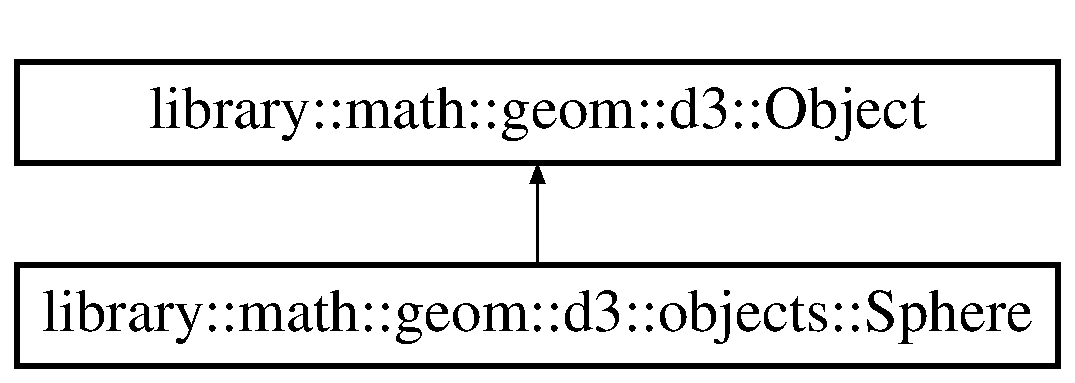
\includegraphics[height=2.000000cm]{classlibrary_1_1math_1_1geom_1_1d3_1_1objects_1_1_sphere}
\end{center}
\end{figure}
\subsection*{Public Member Functions}
\begin{DoxyCompactItemize}
\item 
\hyperlink{classlibrary_1_1math_1_1geom_1_1d3_1_1objects_1_1_sphere_a55dccc8ea16ee55cd7694c26afa8ea39}{Sphere} (const \hyperlink{classlibrary_1_1math_1_1geom_1_1d3_1_1objects_1_1_point}{Point} \&a\+Center, const Real \&a\+Radius)
\begin{DoxyCompactList}\small\item\em Constructor. \end{DoxyCompactList}\item 
virtual \hyperlink{classlibrary_1_1math_1_1geom_1_1d3_1_1objects_1_1_sphere}{Sphere} $\ast$ \hyperlink{classlibrary_1_1math_1_1geom_1_1d3_1_1objects_1_1_sphere_a58370a8ff15b7c5a48cf4ffec5be3015}{clone} () const override
\begin{DoxyCompactList}\small\item\em Clone sphere. \end{DoxyCompactList}\item 
bool \hyperlink{classlibrary_1_1math_1_1geom_1_1d3_1_1objects_1_1_sphere_ace12dcb88802f002f5797077130c4b98}{operator==} (const \hyperlink{classlibrary_1_1math_1_1geom_1_1d3_1_1objects_1_1_sphere}{Sphere} \&a\+Sphere) const
\begin{DoxyCompactList}\small\item\em Equal to operator. \end{DoxyCompactList}\item 
bool \hyperlink{classlibrary_1_1math_1_1geom_1_1d3_1_1objects_1_1_sphere_a127131c48a3bfe342508630cfd399fae}{operator!=} (const \hyperlink{classlibrary_1_1math_1_1geom_1_1d3_1_1objects_1_1_sphere}{Sphere} \&a\+Sphere) const
\begin{DoxyCompactList}\small\item\em Not equal to operator. \end{DoxyCompactList}\item 
virtual bool \hyperlink{classlibrary_1_1math_1_1geom_1_1d3_1_1objects_1_1_sphere_a0598bd75f8a34e07a3ad36cf10a7f098}{is\+Defined} () const override
\begin{DoxyCompactList}\small\item\em Check if sphere is defined. \end{DoxyCompactList}\item 
bool \hyperlink{classlibrary_1_1math_1_1geom_1_1d3_1_1objects_1_1_sphere_a5ec4120b51da519ec14e8bded930b742}{is\+Unitary} () const
\begin{DoxyCompactList}\small\item\em Check if sphere is unitary, i.\+e. its radius is equal to 1.\+0. \end{DoxyCompactList}\item 
\hyperlink{classlibrary_1_1math_1_1geom_1_1d3_1_1objects_1_1_point}{Point} \hyperlink{classlibrary_1_1math_1_1geom_1_1d3_1_1objects_1_1_sphere_a871367ab75aa46194a6b8ddc8a45967f}{get\+Center} () const
\begin{DoxyCompactList}\small\item\em Get sphere center. \end{DoxyCompactList}\item 
Real \hyperlink{classlibrary_1_1math_1_1geom_1_1d3_1_1objects_1_1_sphere_a48cfc72b6eec9a953fb837a13e1df45e}{get\+Radius} () const
\begin{DoxyCompactList}\small\item\em Get sphere radius. \end{DoxyCompactList}\end{DoxyCompactItemize}
\subsection*{Static Public Member Functions}
\begin{DoxyCompactItemize}
\item 
static \hyperlink{classlibrary_1_1math_1_1geom_1_1d3_1_1objects_1_1_sphere}{Sphere} \hyperlink{classlibrary_1_1math_1_1geom_1_1d3_1_1objects_1_1_sphere_a777600f8814a2879e925909f30cfe9c4}{Undefined} ()
\begin{DoxyCompactList}\small\item\em Constructs an undefined sphere. \end{DoxyCompactList}\item 
static \hyperlink{classlibrary_1_1math_1_1geom_1_1d3_1_1objects_1_1_sphere}{Sphere} \hyperlink{classlibrary_1_1math_1_1geom_1_1d3_1_1objects_1_1_sphere_a5464ea9145425db63dedbd896d6c97b0}{Unit} (const \hyperlink{classlibrary_1_1math_1_1geom_1_1d3_1_1objects_1_1_point}{Point} \&a\+Center)
\begin{DoxyCompactList}\small\item\em Constructs a unit sphere. \end{DoxyCompactList}\end{DoxyCompactItemize}
\subsection*{Friends}
\begin{DoxyCompactItemize}
\item 
std\+::ostream \& \hyperlink{classlibrary_1_1math_1_1geom_1_1d3_1_1objects_1_1_sphere_abb141c02e081d1acce5f0d840276a5dd}{operator$<$$<$} (std\+::ostream \&an\+Output\+Stream, const \hyperlink{classlibrary_1_1math_1_1geom_1_1d3_1_1objects_1_1_sphere}{Sphere} \&a\+Sphere)
\begin{DoxyCompactList}\small\item\em Output stream operator. \end{DoxyCompactList}\end{DoxyCompactItemize}


\subsection{Detailed Description}
\hyperlink{classlibrary_1_1math_1_1geom_1_1d3_1_1objects_1_1_sphere}{Sphere}. 

https\+://en.wikipedia.\+org/wiki/\+Sphere 

\subsection{Constructor \& Destructor Documentation}
\mbox{\Hypertarget{classlibrary_1_1math_1_1geom_1_1d3_1_1objects_1_1_sphere_a55dccc8ea16ee55cd7694c26afa8ea39}\label{classlibrary_1_1math_1_1geom_1_1d3_1_1objects_1_1_sphere_a55dccc8ea16ee55cd7694c26afa8ea39}} 
\index{library\+::math\+::geom\+::d3\+::objects\+::\+Sphere@{library\+::math\+::geom\+::d3\+::objects\+::\+Sphere}!Sphere@{Sphere}}
\index{Sphere@{Sphere}!library\+::math\+::geom\+::d3\+::objects\+::\+Sphere@{library\+::math\+::geom\+::d3\+::objects\+::\+Sphere}}
\subsubsection{\texorpdfstring{Sphere()}{Sphere()}}
{\footnotesize\ttfamily library\+::math\+::geom\+::d3\+::objects\+::\+Sphere\+::\+Sphere (\begin{DoxyParamCaption}\item[{const \hyperlink{classlibrary_1_1math_1_1geom_1_1d3_1_1objects_1_1_point}{Point} \&}]{a\+Center,  }\item[{const Real \&}]{a\+Radius }\end{DoxyParamCaption})}



Constructor. 


\begin{DoxyCode}
\hyperlink{classlibrary_1_1math_1_1geom_1_1d3_1_1objects_1_1_sphere_a55dccc8ea16ee55cd7694c26afa8ea39}{Sphere} sphere(\{ 0.0, 0.0, 0.0 \}, 1.0) ;
\end{DoxyCode}



\begin{DoxyParams}[1]{Parameters}
\mbox{\tt in}  & {\em a\+Center} & A sphere center \\
\hline
\mbox{\tt in}  & {\em a\+Radius} & A sphere radius \\
\hline
\end{DoxyParams}


\subsection{Member Function Documentation}
\mbox{\Hypertarget{classlibrary_1_1math_1_1geom_1_1d3_1_1objects_1_1_sphere_a58370a8ff15b7c5a48cf4ffec5be3015}\label{classlibrary_1_1math_1_1geom_1_1d3_1_1objects_1_1_sphere_a58370a8ff15b7c5a48cf4ffec5be3015}} 
\index{library\+::math\+::geom\+::d3\+::objects\+::\+Sphere@{library\+::math\+::geom\+::d3\+::objects\+::\+Sphere}!clone@{clone}}
\index{clone@{clone}!library\+::math\+::geom\+::d3\+::objects\+::\+Sphere@{library\+::math\+::geom\+::d3\+::objects\+::\+Sphere}}
\subsubsection{\texorpdfstring{clone()}{clone()}}
{\footnotesize\ttfamily \hyperlink{classlibrary_1_1math_1_1geom_1_1d3_1_1objects_1_1_sphere}{Sphere} $\ast$ library\+::math\+::geom\+::d3\+::objects\+::\+Sphere\+::clone (\begin{DoxyParamCaption}{ }\end{DoxyParamCaption}) const\hspace{0.3cm}{\ttfamily [override]}, {\ttfamily [virtual]}}



Clone sphere. 

\begin{DoxyReturn}{Returns}
Pointer to cloned sphere 
\end{DoxyReturn}


Implements \hyperlink{classlibrary_1_1math_1_1geom_1_1d3_1_1_object_a1a784c6b359e0eb97cd34fabc42f2f3f}{library\+::math\+::geom\+::d3\+::\+Object}.

\mbox{\Hypertarget{classlibrary_1_1math_1_1geom_1_1d3_1_1objects_1_1_sphere_a871367ab75aa46194a6b8ddc8a45967f}\label{classlibrary_1_1math_1_1geom_1_1d3_1_1objects_1_1_sphere_a871367ab75aa46194a6b8ddc8a45967f}} 
\index{library\+::math\+::geom\+::d3\+::objects\+::\+Sphere@{library\+::math\+::geom\+::d3\+::objects\+::\+Sphere}!get\+Center@{get\+Center}}
\index{get\+Center@{get\+Center}!library\+::math\+::geom\+::d3\+::objects\+::\+Sphere@{library\+::math\+::geom\+::d3\+::objects\+::\+Sphere}}
\subsubsection{\texorpdfstring{get\+Center()}{getCenter()}}
{\footnotesize\ttfamily \hyperlink{classlibrary_1_1math_1_1geom_1_1d3_1_1objects_1_1_point}{Point} library\+::math\+::geom\+::d3\+::objects\+::\+Sphere\+::get\+Center (\begin{DoxyParamCaption}{ }\end{DoxyParamCaption}) const}



Get sphere center. 


\begin{DoxyCode}
\hyperlink{classlibrary_1_1math_1_1geom_1_1d3_1_1objects_1_1_sphere_a55dccc8ea16ee55cd7694c26afa8ea39}{Sphere}(\hyperlink{classlibrary_1_1math_1_1geom_1_1d3_1_1objects_1_1_point_ab2a38e285c562e50bf350272c083986f}{Point::Origin}(), 1.0).getCenter() ; \textcolor{comment}{// [0.0, 0.0, 0.0]}
\end{DoxyCode}


\begin{DoxyReturn}{Returns}
\hyperlink{classlibrary_1_1math_1_1geom_1_1d3_1_1objects_1_1_sphere}{Sphere} center 
\end{DoxyReturn}
\mbox{\Hypertarget{classlibrary_1_1math_1_1geom_1_1d3_1_1objects_1_1_sphere_a48cfc72b6eec9a953fb837a13e1df45e}\label{classlibrary_1_1math_1_1geom_1_1d3_1_1objects_1_1_sphere_a48cfc72b6eec9a953fb837a13e1df45e}} 
\index{library\+::math\+::geom\+::d3\+::objects\+::\+Sphere@{library\+::math\+::geom\+::d3\+::objects\+::\+Sphere}!get\+Radius@{get\+Radius}}
\index{get\+Radius@{get\+Radius}!library\+::math\+::geom\+::d3\+::objects\+::\+Sphere@{library\+::math\+::geom\+::d3\+::objects\+::\+Sphere}}
\subsubsection{\texorpdfstring{get\+Radius()}{getRadius()}}
{\footnotesize\ttfamily Real library\+::math\+::geom\+::d3\+::objects\+::\+Sphere\+::get\+Radius (\begin{DoxyParamCaption}{ }\end{DoxyParamCaption}) const}



Get sphere radius. 


\begin{DoxyCode}
\hyperlink{classlibrary_1_1math_1_1geom_1_1d3_1_1objects_1_1_sphere_a55dccc8ea16ee55cd7694c26afa8ea39}{Sphere}(\hyperlink{classlibrary_1_1math_1_1geom_1_1d3_1_1objects_1_1_point_ab2a38e285c562e50bf350272c083986f}{Point::Origin}(), 1.0).getRadius() ; \textcolor{comment}{// 1.0}
\end{DoxyCode}


\begin{DoxyReturn}{Returns}
\hyperlink{classlibrary_1_1math_1_1geom_1_1d3_1_1objects_1_1_sphere}{Sphere} radius 
\end{DoxyReturn}
\mbox{\Hypertarget{classlibrary_1_1math_1_1geom_1_1d3_1_1objects_1_1_sphere_a0598bd75f8a34e07a3ad36cf10a7f098}\label{classlibrary_1_1math_1_1geom_1_1d3_1_1objects_1_1_sphere_a0598bd75f8a34e07a3ad36cf10a7f098}} 
\index{library\+::math\+::geom\+::d3\+::objects\+::\+Sphere@{library\+::math\+::geom\+::d3\+::objects\+::\+Sphere}!is\+Defined@{is\+Defined}}
\index{is\+Defined@{is\+Defined}!library\+::math\+::geom\+::d3\+::objects\+::\+Sphere@{library\+::math\+::geom\+::d3\+::objects\+::\+Sphere}}
\subsubsection{\texorpdfstring{is\+Defined()}{isDefined()}}
{\footnotesize\ttfamily bool library\+::math\+::geom\+::d3\+::objects\+::\+Sphere\+::is\+Defined (\begin{DoxyParamCaption}{ }\end{DoxyParamCaption}) const\hspace{0.3cm}{\ttfamily [override]}, {\ttfamily [virtual]}}



Check if sphere is defined. 


\begin{DoxyCode}
\hyperlink{classlibrary_1_1math_1_1geom_1_1d3_1_1objects_1_1_sphere_a55dccc8ea16ee55cd7694c26afa8ea39}{Sphere}(\hyperlink{classlibrary_1_1math_1_1geom_1_1d3_1_1objects_1_1_point_ab2a38e285c562e50bf350272c083986f}{Point::Origin}(), 1.0).isDefined() ; \textcolor{comment}{// True}
\end{DoxyCode}


\begin{DoxyReturn}{Returns}
True if sphere is defined 
\end{DoxyReturn}


Implements \hyperlink{classlibrary_1_1math_1_1geom_1_1d3_1_1_object_a2216442e322f0c3ca5f01a4efa22baf7}{library\+::math\+::geom\+::d3\+::\+Object}.

\mbox{\Hypertarget{classlibrary_1_1math_1_1geom_1_1d3_1_1objects_1_1_sphere_a5ec4120b51da519ec14e8bded930b742}\label{classlibrary_1_1math_1_1geom_1_1d3_1_1objects_1_1_sphere_a5ec4120b51da519ec14e8bded930b742}} 
\index{library\+::math\+::geom\+::d3\+::objects\+::\+Sphere@{library\+::math\+::geom\+::d3\+::objects\+::\+Sphere}!is\+Unitary@{is\+Unitary}}
\index{is\+Unitary@{is\+Unitary}!library\+::math\+::geom\+::d3\+::objects\+::\+Sphere@{library\+::math\+::geom\+::d3\+::objects\+::\+Sphere}}
\subsubsection{\texorpdfstring{is\+Unitary()}{isUnitary()}}
{\footnotesize\ttfamily bool library\+::math\+::geom\+::d3\+::objects\+::\+Sphere\+::is\+Unitary (\begin{DoxyParamCaption}{ }\end{DoxyParamCaption}) const}



Check if sphere is unitary, i.\+e. its radius is equal to 1.\+0. 


\begin{DoxyCode}
\hyperlink{classlibrary_1_1math_1_1geom_1_1d3_1_1objects_1_1_sphere_a55dccc8ea16ee55cd7694c26afa8ea39}{Sphere}(\hyperlink{classlibrary_1_1math_1_1geom_1_1d3_1_1objects_1_1_point_ab2a38e285c562e50bf350272c083986f}{Point::Origin}(), 1.0).isUnitary() ; \textcolor{comment}{// True}
\end{DoxyCode}


\begin{DoxyReturn}{Returns}
True if sphere is unitary 
\end{DoxyReturn}
\mbox{\Hypertarget{classlibrary_1_1math_1_1geom_1_1d3_1_1objects_1_1_sphere_a127131c48a3bfe342508630cfd399fae}\label{classlibrary_1_1math_1_1geom_1_1d3_1_1objects_1_1_sphere_a127131c48a3bfe342508630cfd399fae}} 
\index{library\+::math\+::geom\+::d3\+::objects\+::\+Sphere@{library\+::math\+::geom\+::d3\+::objects\+::\+Sphere}!operator"!=@{operator"!=}}
\index{operator"!=@{operator"!=}!library\+::math\+::geom\+::d3\+::objects\+::\+Sphere@{library\+::math\+::geom\+::d3\+::objects\+::\+Sphere}}
\subsubsection{\texorpdfstring{operator"!=()}{operator!=()}}
{\footnotesize\ttfamily bool library\+::math\+::geom\+::d3\+::objects\+::\+Sphere\+::operator!= (\begin{DoxyParamCaption}\item[{const \hyperlink{classlibrary_1_1math_1_1geom_1_1d3_1_1objects_1_1_sphere}{Sphere} \&}]{a\+Sphere }\end{DoxyParamCaption}) const}



Not equal to operator. 


\begin{DoxyCode}
\hyperlink{classlibrary_1_1math_1_1geom_1_1d3_1_1objects_1_1_sphere_a55dccc8ea16ee55cd7694c26afa8ea39}{Sphere}(\hyperlink{classlibrary_1_1math_1_1geom_1_1d3_1_1objects_1_1_point_ab2a38e285c562e50bf350272c083986f}{Point::Origin}(), 1.0) != \hyperlink{classlibrary_1_1math_1_1geom_1_1d3_1_1objects_1_1_sphere_a55dccc8ea16ee55cd7694c26afa8ea39}{Sphere}(2.0) ; \textcolor{comment}{// True}
\end{DoxyCode}



\begin{DoxyParams}[1]{Parameters}
\mbox{\tt in}  & {\em a\+Sphere} & A sphere \\
\hline
\end{DoxyParams}
\begin{DoxyReturn}{Returns}
True if spheres not are equal 
\end{DoxyReturn}
\mbox{\Hypertarget{classlibrary_1_1math_1_1geom_1_1d3_1_1objects_1_1_sphere_ace12dcb88802f002f5797077130c4b98}\label{classlibrary_1_1math_1_1geom_1_1d3_1_1objects_1_1_sphere_ace12dcb88802f002f5797077130c4b98}} 
\index{library\+::math\+::geom\+::d3\+::objects\+::\+Sphere@{library\+::math\+::geom\+::d3\+::objects\+::\+Sphere}!operator==@{operator==}}
\index{operator==@{operator==}!library\+::math\+::geom\+::d3\+::objects\+::\+Sphere@{library\+::math\+::geom\+::d3\+::objects\+::\+Sphere}}
\subsubsection{\texorpdfstring{operator==()}{operator==()}}
{\footnotesize\ttfamily bool library\+::math\+::geom\+::d3\+::objects\+::\+Sphere\+::operator== (\begin{DoxyParamCaption}\item[{const \hyperlink{classlibrary_1_1math_1_1geom_1_1d3_1_1objects_1_1_sphere}{Sphere} \&}]{a\+Sphere }\end{DoxyParamCaption}) const}



Equal to operator. 


\begin{DoxyCode}
\hyperlink{classlibrary_1_1math_1_1geom_1_1d3_1_1objects_1_1_sphere_a55dccc8ea16ee55cd7694c26afa8ea39}{Sphere}(\hyperlink{classlibrary_1_1math_1_1geom_1_1d3_1_1objects_1_1_point_ab2a38e285c562e50bf350272c083986f}{Point::Origin}(), 1.0) == \hyperlink{classlibrary_1_1math_1_1geom_1_1d3_1_1objects_1_1_sphere_a55dccc8ea16ee55cd7694c26afa8ea39}{Sphere}(\hyperlink{classlibrary_1_1math_1_1geom_1_1d3_1_1objects_1_1_point_ab2a38e285c562e50bf350272c083986f}{Point::Origin}(), 1.0) ; \textcolor{comment}{//
       True}
\end{DoxyCode}



\begin{DoxyParams}[1]{Parameters}
\mbox{\tt in}  & {\em a\+Sphere} & A sphere \\
\hline
\end{DoxyParams}
\begin{DoxyReturn}{Returns}
True if spheres are equal 
\end{DoxyReturn}
\mbox{\Hypertarget{classlibrary_1_1math_1_1geom_1_1d3_1_1objects_1_1_sphere_a777600f8814a2879e925909f30cfe9c4}\label{classlibrary_1_1math_1_1geom_1_1d3_1_1objects_1_1_sphere_a777600f8814a2879e925909f30cfe9c4}} 
\index{library\+::math\+::geom\+::d3\+::objects\+::\+Sphere@{library\+::math\+::geom\+::d3\+::objects\+::\+Sphere}!Undefined@{Undefined}}
\index{Undefined@{Undefined}!library\+::math\+::geom\+::d3\+::objects\+::\+Sphere@{library\+::math\+::geom\+::d3\+::objects\+::\+Sphere}}
\subsubsection{\texorpdfstring{Undefined()}{Undefined()}}
{\footnotesize\ttfamily \hyperlink{classlibrary_1_1math_1_1geom_1_1d3_1_1objects_1_1_sphere}{Sphere} library\+::math\+::geom\+::d3\+::objects\+::\+Sphere\+::\+Undefined (\begin{DoxyParamCaption}{ }\end{DoxyParamCaption})\hspace{0.3cm}{\ttfamily [static]}}



Constructs an undefined sphere. 


\begin{DoxyCode}
\hyperlink{classlibrary_1_1math_1_1geom_1_1d3_1_1objects_1_1_sphere_a55dccc8ea16ee55cd7694c26afa8ea39}{Sphere} sphere = \hyperlink{classlibrary_1_1math_1_1geom_1_1d3_1_1objects_1_1_sphere_a777600f8814a2879e925909f30cfe9c4}{Sphere::Undefined}() ; \textcolor{comment}{// Undefined}
\end{DoxyCode}


\begin{DoxyReturn}{Returns}
Undefined sphere 
\end{DoxyReturn}
\mbox{\Hypertarget{classlibrary_1_1math_1_1geom_1_1d3_1_1objects_1_1_sphere_a5464ea9145425db63dedbd896d6c97b0}\label{classlibrary_1_1math_1_1geom_1_1d3_1_1objects_1_1_sphere_a5464ea9145425db63dedbd896d6c97b0}} 
\index{library\+::math\+::geom\+::d3\+::objects\+::\+Sphere@{library\+::math\+::geom\+::d3\+::objects\+::\+Sphere}!Unit@{Unit}}
\index{Unit@{Unit}!library\+::math\+::geom\+::d3\+::objects\+::\+Sphere@{library\+::math\+::geom\+::d3\+::objects\+::\+Sphere}}
\subsubsection{\texorpdfstring{Unit()}{Unit()}}
{\footnotesize\ttfamily \hyperlink{classlibrary_1_1math_1_1geom_1_1d3_1_1objects_1_1_sphere}{Sphere} library\+::math\+::geom\+::d3\+::objects\+::\+Sphere\+::\+Unit (\begin{DoxyParamCaption}\item[{const \hyperlink{classlibrary_1_1math_1_1geom_1_1d3_1_1objects_1_1_point}{Point} \&}]{a\+Center }\end{DoxyParamCaption})\hspace{0.3cm}{\ttfamily [static]}}



Constructs a unit sphere. 

https\+://en.wikipedia.\+org/wiki/\+Unit\+\_\+sphere


\begin{DoxyCode}
\hyperlink{classlibrary_1_1math_1_1geom_1_1d3_1_1objects_1_1_sphere_a55dccc8ea16ee55cd7694c26afa8ea39}{Sphere} sphere = \hyperlink{classlibrary_1_1math_1_1geom_1_1d3_1_1objects_1_1_sphere_a5464ea9145425db63dedbd896d6c97b0}{Sphere::Unit}(\{ 0.0, 0.0, 0.0 \}) ;
\end{DoxyCode}


\begin{DoxyReturn}{Returns}
Unit sphere 
\end{DoxyReturn}


\subsection{Friends And Related Function Documentation}
\mbox{\Hypertarget{classlibrary_1_1math_1_1geom_1_1d3_1_1objects_1_1_sphere_abb141c02e081d1acce5f0d840276a5dd}\label{classlibrary_1_1math_1_1geom_1_1d3_1_1objects_1_1_sphere_abb141c02e081d1acce5f0d840276a5dd}} 
\index{library\+::math\+::geom\+::d3\+::objects\+::\+Sphere@{library\+::math\+::geom\+::d3\+::objects\+::\+Sphere}!operator$<$$<$@{operator$<$$<$}}
\index{operator$<$$<$@{operator$<$$<$}!library\+::math\+::geom\+::d3\+::objects\+::\+Sphere@{library\+::math\+::geom\+::d3\+::objects\+::\+Sphere}}
\subsubsection{\texorpdfstring{operator$<$$<$}{operator<<}}
{\footnotesize\ttfamily std\+::ostream\& operator$<$$<$ (\begin{DoxyParamCaption}\item[{std\+::ostream \&}]{an\+Output\+Stream,  }\item[{const \hyperlink{classlibrary_1_1math_1_1geom_1_1d3_1_1objects_1_1_sphere}{Sphere} \&}]{a\+Sphere }\end{DoxyParamCaption})\hspace{0.3cm}{\ttfamily [friend]}}



Output stream operator. 


\begin{DoxyCode}
std::cout << \hyperlink{classlibrary_1_1math_1_1geom_1_1d3_1_1objects_1_1_sphere_a55dccc8ea16ee55cd7694c26afa8ea39}{Sphere}(\hyperlink{classlibrary_1_1math_1_1geom_1_1d3_1_1objects_1_1_point_ab2a38e285c562e50bf350272c083986f}{Point::Origin}(), 1.0) ;
\end{DoxyCode}



\begin{DoxyParams}[1]{Parameters}
\mbox{\tt in}  & {\em an\+Output\+Stream} & An output stream \\
\hline
\mbox{\tt in}  & {\em a\+Sphere} & A sphere \\
\hline
\end{DoxyParams}
\begin{DoxyReturn}{Returns}
An output stream 
\end{DoxyReturn}


The documentation for this class was generated from the following files\+:\begin{DoxyCompactItemize}
\item 
include/\+Library/\+Mathematics/\+Geometry/3\+D/\+Objects/\hyperlink{_sphere_8hpp}{Sphere.\+hpp}\item 
src/\+Library/\+Mathematics/\+Geometry/3\+D/\+Objects/\hyperlink{_sphere_8cpp}{Sphere.\+cpp}\end{DoxyCompactItemize}

\hypertarget{classlibrary_1_1math_1_1geom_1_1d3_1_1_transformation}{}\section{library\+:\+:math\+:\+:geom\+:\+:d3\+:\+:Transformation Class Reference}
\label{classlibrary_1_1math_1_1geom_1_1d3_1_1_transformation}\index{library\+::math\+::geom\+::d3\+::\+Transformation@{library\+::math\+::geom\+::d3\+::\+Transformation}}


{\ttfamily \#include $<$Transformation.\+hpp$>$}

\subsection*{Public Types}
\begin{DoxyCompactItemize}
\item 
enum \hyperlink{classlibrary_1_1math_1_1geom_1_1d3_1_1_transformation_a25f1dc99d391174bf82a7132d08b2fc1}{Type} \{ \newline
\hyperlink{classlibrary_1_1math_1_1geom_1_1d3_1_1_transformation_a25f1dc99d391174bf82a7132d08b2fc1aec0fc0100c4fc1ce4eea230c3dc10360}{Type\+::\+Undefined}, 
\hyperlink{classlibrary_1_1math_1_1geom_1_1d3_1_1_transformation_a25f1dc99d391174bf82a7132d08b2fc1ac9c5c65fb4af9cf90eb99b3b84424189}{Type\+::\+Identity}, 
\hyperlink{classlibrary_1_1math_1_1geom_1_1d3_1_1_transformation_a25f1dc99d391174bf82a7132d08b2fc1a6dd08874f83507e9c7b23f1a46b7fa7c}{Type\+::\+Translation}, 
\hyperlink{classlibrary_1_1math_1_1geom_1_1d3_1_1_transformation_a25f1dc99d391174bf82a7132d08b2fc1af1a42bd417390fc63b030a519624607a}{Type\+::\+Rotation}, 
\newline
\hyperlink{classlibrary_1_1math_1_1geom_1_1d3_1_1_transformation_a25f1dc99d391174bf82a7132d08b2fc1abc967dc2d57e6eff184a821bf7577a80}{Type\+::\+Scaling}, 
\hyperlink{classlibrary_1_1math_1_1geom_1_1d3_1_1_transformation_a25f1dc99d391174bf82a7132d08b2fc1aaea1e492943ccbad7ee270ec1e064758}{Type\+::\+Reflection}, 
\hyperlink{classlibrary_1_1math_1_1geom_1_1d3_1_1_transformation_a25f1dc99d391174bf82a7132d08b2fc1a02414922b70cc0f9d7c841b0c70a0f94}{Type\+::\+Shear}, 
\hyperlink{classlibrary_1_1math_1_1geom_1_1d3_1_1_transformation_a25f1dc99d391174bf82a7132d08b2fc1a5b525aab6e200981a842101f1bcbafc6}{Type\+::\+Affine}
 \}
\end{DoxyCompactItemize}
\subsection*{Public Member Functions}
\begin{DoxyCompactItemize}
\item 
\hyperlink{classlibrary_1_1math_1_1geom_1_1d3_1_1_transformation_ac98131fb82e06d5d5ee3b9d5c8981834}{Transformation} (const Matrix4d \&a\+Matrix)
\begin{DoxyCompactList}\small\item\em Constructor. \end{DoxyCompactList}\item 
bool \hyperlink{classlibrary_1_1math_1_1geom_1_1d3_1_1_transformation_ad65ef7737c9299ae939585873a147800}{operator==} (const \hyperlink{classlibrary_1_1math_1_1geom_1_1d3_1_1_transformation}{Transformation} \&a\+Transformation) const
\item 
bool \hyperlink{classlibrary_1_1math_1_1geom_1_1d3_1_1_transformation_ac231beeb8ada73eada915903af7c56b1}{operator!=} (const \hyperlink{classlibrary_1_1math_1_1geom_1_1d3_1_1_transformation}{Transformation} \&a\+Transformation) const
\item 
\hyperlink{classlibrary_1_1math_1_1geom_1_1d3_1_1_transformation}{Transformation} \hyperlink{classlibrary_1_1math_1_1geom_1_1d3_1_1_transformation_ad2ac7373f1e8a55ca22da045a5853c18}{operator$\ast$} (const \hyperlink{classlibrary_1_1math_1_1geom_1_1d3_1_1_transformation}{Transformation} \&a\+Transformation) const
\item 
Vector4d \hyperlink{classlibrary_1_1math_1_1geom_1_1d3_1_1_transformation_a17ea83976590631f71837398fc59f1ac}{operator$\ast$} (const Vector4d \&a\+Vector) const
\item 
\hyperlink{classlibrary_1_1math_1_1geom_1_1d3_1_1_transformation}{Transformation} \& \hyperlink{classlibrary_1_1math_1_1geom_1_1d3_1_1_transformation_ae0b9940900e14241a1fb074ada53e344}{operator$\ast$=} (const \hyperlink{classlibrary_1_1math_1_1geom_1_1d3_1_1_transformation}{Transformation} \&a\+Transformation)
\item 
bool \hyperlink{classlibrary_1_1math_1_1geom_1_1d3_1_1_transformation_ac8d339a3e975939cf0ea37bbff0ba53d}{is\+Defined} () const
\item 
bool \hyperlink{classlibrary_1_1math_1_1geom_1_1d3_1_1_transformation_ac315d6665d1a589995b8ac3501edb668}{is\+Identity} () const
\item 
bool \hyperlink{classlibrary_1_1math_1_1geom_1_1d3_1_1_transformation_a21d2c767561d59c1fc53cdc254207971}{is\+Rigid} () const
\begin{DoxyCompactList}\small\item\em Returns true if transformation is rigid. \end{DoxyCompactList}\item 
\hyperlink{classlibrary_1_1math_1_1geom_1_1d3_1_1_transformation_a25f1dc99d391174bf82a7132d08b2fc1}{Transformation\+::\+Type} \hyperlink{classlibrary_1_1math_1_1geom_1_1d3_1_1_transformation_a719b99d5613e2070007e19364b0ec7ac}{get\+Type} () const
\item 
Matrix4d \hyperlink{classlibrary_1_1math_1_1geom_1_1d3_1_1_transformation_ace5db8c23a30c09ace877d7e5f79695e}{get\+Matrix} () const
\item 
\hyperlink{classlibrary_1_1math_1_1geom_1_1d3_1_1_transformation}{Transformation} \hyperlink{classlibrary_1_1math_1_1geom_1_1d3_1_1_transformation_a4e3bd6d4533bb6bcb5ec5e66fcf53db4}{get\+Inverse} () const
\item 
\hyperlink{classlibrary_1_1math_1_1geom_1_1d3_1_1objects_1_1_point}{Point} \hyperlink{classlibrary_1_1math_1_1geom_1_1d3_1_1_transformation_aa6e1d09d2c3c45dda7179118a1969238}{apply\+To} (const \hyperlink{classlibrary_1_1math_1_1geom_1_1d3_1_1objects_1_1_point}{Point} \&a\+Point) const
\item 
Vector3d \hyperlink{classlibrary_1_1math_1_1geom_1_1d3_1_1_transformation_ac5fb182db7d89722baafa37b074ba44c}{apply\+To} (const Vector3d \&a\+Vector) const
\item 
virtual void \hyperlink{classlibrary_1_1math_1_1geom_1_1d3_1_1_transformation_a0cafbc8affb176f6774af01b98536e69}{print} (std\+::ostream \&an\+Output\+Stream, bool display\+Decorators=true) const
\begin{DoxyCompactList}\small\item\em Print transformation. \end{DoxyCompactList}\end{DoxyCompactItemize}
\subsection*{Static Public Member Functions}
\begin{DoxyCompactItemize}
\item 
static \hyperlink{classlibrary_1_1math_1_1geom_1_1d3_1_1_transformation}{Transformation} \hyperlink{classlibrary_1_1math_1_1geom_1_1d3_1_1_transformation_acb7375bde02ed5832d5937908bee7043}{Undefined} ()
\item 
static \hyperlink{classlibrary_1_1math_1_1geom_1_1d3_1_1_transformation}{Transformation} \hyperlink{classlibrary_1_1math_1_1geom_1_1d3_1_1_transformation_a8d5af972dbba51f5746f2248f5164b69}{Identity} ()
\item 
static \hyperlink{classlibrary_1_1math_1_1geom_1_1d3_1_1_transformation}{Transformation} \hyperlink{classlibrary_1_1math_1_1geom_1_1d3_1_1_transformation_a5f781ba4e25ce79a02afccbe94a1ab0a}{Translation} (const Vector3d \&a\+Translation\+Vector)
\item 
static \hyperlink{classlibrary_1_1math_1_1geom_1_1d3_1_1_transformation}{Transformation} \hyperlink{classlibrary_1_1math_1_1geom_1_1d3_1_1_transformation_a79978a6efb749a2e058aa0b2cea092b2}{Rotation} (const \hyperlink{classlibrary_1_1math_1_1geom_1_1trf_1_1rot_1_1_rotation_vector}{Rotation\+Vector} \&a\+Rotation\+Vector)
\item 
static \hyperlink{classlibrary_1_1math_1_1geom_1_1d3_1_1_transformation}{Transformation} \hyperlink{classlibrary_1_1math_1_1geom_1_1d3_1_1_transformation_a11d93f665adb24cc4fdf2244c8509082}{Rotation\+Around} (const \hyperlink{classlibrary_1_1math_1_1geom_1_1d3_1_1objects_1_1_point}{Point} \&a\+Point, const \hyperlink{classlibrary_1_1math_1_1geom_1_1trf_1_1rot_1_1_rotation_vector}{Rotation\+Vector} \&a\+Rotation\+Vector)
\item 
static String \hyperlink{classlibrary_1_1math_1_1geom_1_1d3_1_1_transformation_a9511c7844b5b8af0c8c7ad97454a5a96}{String\+From\+Type} (const \hyperlink{classlibrary_1_1math_1_1geom_1_1d3_1_1_transformation_a25f1dc99d391174bf82a7132d08b2fc1}{Transformation\+::\+Type} \&a\+Type)
\item 
static \hyperlink{classlibrary_1_1math_1_1geom_1_1d3_1_1_transformation_a25f1dc99d391174bf82a7132d08b2fc1}{Transformation\+::\+Type} \hyperlink{classlibrary_1_1math_1_1geom_1_1d3_1_1_transformation_aa532f2c9f56ee5aff63417283a930584}{Type\+Of\+Matrix} (const Matrix4d \&a\+Matrix)
\end{DoxyCompactItemize}
\subsection*{Friends}
\begin{DoxyCompactItemize}
\item 
std\+::ostream \& \hyperlink{classlibrary_1_1math_1_1geom_1_1d3_1_1_transformation_afb2829e106dc4aeab1c706d1eaa357e8}{operator$<$$<$} (std\+::ostream \&an\+Output\+Stream, const \hyperlink{classlibrary_1_1math_1_1geom_1_1d3_1_1_transformation}{Transformation} \&a\+Transformation)
\end{DoxyCompactItemize}


\subsection{Member Enumeration Documentation}
\mbox{\Hypertarget{classlibrary_1_1math_1_1geom_1_1d3_1_1_transformation_a25f1dc99d391174bf82a7132d08b2fc1}\label{classlibrary_1_1math_1_1geom_1_1d3_1_1_transformation_a25f1dc99d391174bf82a7132d08b2fc1}} 
\index{library\+::math\+::geom\+::d3\+::\+Transformation@{library\+::math\+::geom\+::d3\+::\+Transformation}!Type@{Type}}
\index{Type@{Type}!library\+::math\+::geom\+::d3\+::\+Transformation@{library\+::math\+::geom\+::d3\+::\+Transformation}}
\subsubsection{\texorpdfstring{Type}{Type}}
{\footnotesize\ttfamily enum \hyperlink{classlibrary_1_1math_1_1geom_1_1d3_1_1_transformation_a25f1dc99d391174bf82a7132d08b2fc1}{library\+::math\+::geom\+::d3\+::\+Transformation\+::\+Type}\hspace{0.3cm}{\ttfamily [strong]}}

\begin{DoxyEnumFields}{Enumerator}
\raisebox{\heightof{T}}[0pt][0pt]{\index{Undefined@{Undefined}!library\+::math\+::geom\+::d3\+::\+Transformation@{library\+::math\+::geom\+::d3\+::\+Transformation}}\index{library\+::math\+::geom\+::d3\+::\+Transformation@{library\+::math\+::geom\+::d3\+::\+Transformation}!Undefined@{Undefined}}}\mbox{\Hypertarget{classlibrary_1_1math_1_1geom_1_1d3_1_1_transformation_a25f1dc99d391174bf82a7132d08b2fc1aec0fc0100c4fc1ce4eea230c3dc10360}\label{classlibrary_1_1math_1_1geom_1_1d3_1_1_transformation_a25f1dc99d391174bf82a7132d08b2fc1aec0fc0100c4fc1ce4eea230c3dc10360}} 
Undefined&\\
\hline

\raisebox{\heightof{T}}[0pt][0pt]{\index{Identity@{Identity}!library\+::math\+::geom\+::d3\+::\+Transformation@{library\+::math\+::geom\+::d3\+::\+Transformation}}\index{library\+::math\+::geom\+::d3\+::\+Transformation@{library\+::math\+::geom\+::d3\+::\+Transformation}!Identity@{Identity}}}\mbox{\Hypertarget{classlibrary_1_1math_1_1geom_1_1d3_1_1_transformation_a25f1dc99d391174bf82a7132d08b2fc1ac9c5c65fb4af9cf90eb99b3b84424189}\label{classlibrary_1_1math_1_1geom_1_1d3_1_1_transformation_a25f1dc99d391174bf82a7132d08b2fc1ac9c5c65fb4af9cf90eb99b3b84424189}} 
Identity&\\
\hline

\raisebox{\heightof{T}}[0pt][0pt]{\index{Translation@{Translation}!library\+::math\+::geom\+::d3\+::\+Transformation@{library\+::math\+::geom\+::d3\+::\+Transformation}}\index{library\+::math\+::geom\+::d3\+::\+Transformation@{library\+::math\+::geom\+::d3\+::\+Transformation}!Translation@{Translation}}}\mbox{\Hypertarget{classlibrary_1_1math_1_1geom_1_1d3_1_1_transformation_a25f1dc99d391174bf82a7132d08b2fc1a6dd08874f83507e9c7b23f1a46b7fa7c}\label{classlibrary_1_1math_1_1geom_1_1d3_1_1_transformation_a25f1dc99d391174bf82a7132d08b2fc1a6dd08874f83507e9c7b23f1a46b7fa7c}} 
Translation&\\
\hline

\raisebox{\heightof{T}}[0pt][0pt]{\index{Rotation@{Rotation}!library\+::math\+::geom\+::d3\+::\+Transformation@{library\+::math\+::geom\+::d3\+::\+Transformation}}\index{library\+::math\+::geom\+::d3\+::\+Transformation@{library\+::math\+::geom\+::d3\+::\+Transformation}!Rotation@{Rotation}}}\mbox{\Hypertarget{classlibrary_1_1math_1_1geom_1_1d3_1_1_transformation_a25f1dc99d391174bf82a7132d08b2fc1af1a42bd417390fc63b030a519624607a}\label{classlibrary_1_1math_1_1geom_1_1d3_1_1_transformation_a25f1dc99d391174bf82a7132d08b2fc1af1a42bd417390fc63b030a519624607a}} 
Rotation&\\
\hline

\raisebox{\heightof{T}}[0pt][0pt]{\index{Scaling@{Scaling}!library\+::math\+::geom\+::d3\+::\+Transformation@{library\+::math\+::geom\+::d3\+::\+Transformation}}\index{library\+::math\+::geom\+::d3\+::\+Transformation@{library\+::math\+::geom\+::d3\+::\+Transformation}!Scaling@{Scaling}}}\mbox{\Hypertarget{classlibrary_1_1math_1_1geom_1_1d3_1_1_transformation_a25f1dc99d391174bf82a7132d08b2fc1abc967dc2d57e6eff184a821bf7577a80}\label{classlibrary_1_1math_1_1geom_1_1d3_1_1_transformation_a25f1dc99d391174bf82a7132d08b2fc1abc967dc2d57e6eff184a821bf7577a80}} 
Scaling&\\
\hline

\raisebox{\heightof{T}}[0pt][0pt]{\index{Reflection@{Reflection}!library\+::math\+::geom\+::d3\+::\+Transformation@{library\+::math\+::geom\+::d3\+::\+Transformation}}\index{library\+::math\+::geom\+::d3\+::\+Transformation@{library\+::math\+::geom\+::d3\+::\+Transformation}!Reflection@{Reflection}}}\mbox{\Hypertarget{classlibrary_1_1math_1_1geom_1_1d3_1_1_transformation_a25f1dc99d391174bf82a7132d08b2fc1aaea1e492943ccbad7ee270ec1e064758}\label{classlibrary_1_1math_1_1geom_1_1d3_1_1_transformation_a25f1dc99d391174bf82a7132d08b2fc1aaea1e492943ccbad7ee270ec1e064758}} 
Reflection&\\
\hline

\raisebox{\heightof{T}}[0pt][0pt]{\index{Shear@{Shear}!library\+::math\+::geom\+::d3\+::\+Transformation@{library\+::math\+::geom\+::d3\+::\+Transformation}}\index{library\+::math\+::geom\+::d3\+::\+Transformation@{library\+::math\+::geom\+::d3\+::\+Transformation}!Shear@{Shear}}}\mbox{\Hypertarget{classlibrary_1_1math_1_1geom_1_1d3_1_1_transformation_a25f1dc99d391174bf82a7132d08b2fc1a02414922b70cc0f9d7c841b0c70a0f94}\label{classlibrary_1_1math_1_1geom_1_1d3_1_1_transformation_a25f1dc99d391174bf82a7132d08b2fc1a02414922b70cc0f9d7c841b0c70a0f94}} 
Shear&\\
\hline

\raisebox{\heightof{T}}[0pt][0pt]{\index{Affine@{Affine}!library\+::math\+::geom\+::d3\+::\+Transformation@{library\+::math\+::geom\+::d3\+::\+Transformation}}\index{library\+::math\+::geom\+::d3\+::\+Transformation@{library\+::math\+::geom\+::d3\+::\+Transformation}!Affine@{Affine}}}\mbox{\Hypertarget{classlibrary_1_1math_1_1geom_1_1d3_1_1_transformation_a25f1dc99d391174bf82a7132d08b2fc1a5b525aab6e200981a842101f1bcbafc6}\label{classlibrary_1_1math_1_1geom_1_1d3_1_1_transformation_a25f1dc99d391174bf82a7132d08b2fc1a5b525aab6e200981a842101f1bcbafc6}} 
Affine&\\
\hline

\end{DoxyEnumFields}


\subsection{Constructor \& Destructor Documentation}
\mbox{\Hypertarget{classlibrary_1_1math_1_1geom_1_1d3_1_1_transformation_ac98131fb82e06d5d5ee3b9d5c8981834}\label{classlibrary_1_1math_1_1geom_1_1d3_1_1_transformation_ac98131fb82e06d5d5ee3b9d5c8981834}} 
\index{library\+::math\+::geom\+::d3\+::\+Transformation@{library\+::math\+::geom\+::d3\+::\+Transformation}!Transformation@{Transformation}}
\index{Transformation@{Transformation}!library\+::math\+::geom\+::d3\+::\+Transformation@{library\+::math\+::geom\+::d3\+::\+Transformation}}
\subsubsection{\texorpdfstring{Transformation()}{Transformation()}}
{\footnotesize\ttfamily library\+::math\+::geom\+::d3\+::\+Transformation\+::\+Transformation (\begin{DoxyParamCaption}\item[{const Matrix4d \&}]{a\+Matrix }\end{DoxyParamCaption})}



Constructor. 


\begin{DoxyParams}[1]{Parameters}
\mbox{\tt in}  & {\em a\+Matrix} & A transformation matrix \\
\hline
\end{DoxyParams}


\subsection{Member Function Documentation}
\mbox{\Hypertarget{classlibrary_1_1math_1_1geom_1_1d3_1_1_transformation_aa6e1d09d2c3c45dda7179118a1969238}\label{classlibrary_1_1math_1_1geom_1_1d3_1_1_transformation_aa6e1d09d2c3c45dda7179118a1969238}} 
\index{library\+::math\+::geom\+::d3\+::\+Transformation@{library\+::math\+::geom\+::d3\+::\+Transformation}!apply\+To@{apply\+To}}
\index{apply\+To@{apply\+To}!library\+::math\+::geom\+::d3\+::\+Transformation@{library\+::math\+::geom\+::d3\+::\+Transformation}}
\subsubsection{\texorpdfstring{apply\+To()}{applyTo()}\hspace{0.1cm}{\footnotesize\ttfamily [1/2]}}
{\footnotesize\ttfamily \hyperlink{classlibrary_1_1math_1_1geom_1_1d3_1_1objects_1_1_point}{Point} library\+::math\+::geom\+::d3\+::\+Transformation\+::apply\+To (\begin{DoxyParamCaption}\item[{const \hyperlink{classlibrary_1_1math_1_1geom_1_1d3_1_1objects_1_1_point}{Point} \&}]{a\+Point }\end{DoxyParamCaption}) const}

\mbox{\Hypertarget{classlibrary_1_1math_1_1geom_1_1d3_1_1_transformation_ac5fb182db7d89722baafa37b074ba44c}\label{classlibrary_1_1math_1_1geom_1_1d3_1_1_transformation_ac5fb182db7d89722baafa37b074ba44c}} 
\index{library\+::math\+::geom\+::d3\+::\+Transformation@{library\+::math\+::geom\+::d3\+::\+Transformation}!apply\+To@{apply\+To}}
\index{apply\+To@{apply\+To}!library\+::math\+::geom\+::d3\+::\+Transformation@{library\+::math\+::geom\+::d3\+::\+Transformation}}
\subsubsection{\texorpdfstring{apply\+To()}{applyTo()}\hspace{0.1cm}{\footnotesize\ttfamily [2/2]}}
{\footnotesize\ttfamily Vector3d library\+::math\+::geom\+::d3\+::\+Transformation\+::apply\+To (\begin{DoxyParamCaption}\item[{const Vector3d \&}]{a\+Vector }\end{DoxyParamCaption}) const}

\mbox{\Hypertarget{classlibrary_1_1math_1_1geom_1_1d3_1_1_transformation_a4e3bd6d4533bb6bcb5ec5e66fcf53db4}\label{classlibrary_1_1math_1_1geom_1_1d3_1_1_transformation_a4e3bd6d4533bb6bcb5ec5e66fcf53db4}} 
\index{library\+::math\+::geom\+::d3\+::\+Transformation@{library\+::math\+::geom\+::d3\+::\+Transformation}!get\+Inverse@{get\+Inverse}}
\index{get\+Inverse@{get\+Inverse}!library\+::math\+::geom\+::d3\+::\+Transformation@{library\+::math\+::geom\+::d3\+::\+Transformation}}
\subsubsection{\texorpdfstring{get\+Inverse()}{getInverse()}}
{\footnotesize\ttfamily \hyperlink{classlibrary_1_1math_1_1geom_1_1d3_1_1_transformation}{Transformation} library\+::math\+::geom\+::d3\+::\+Transformation\+::get\+Inverse (\begin{DoxyParamCaption}{ }\end{DoxyParamCaption}) const}

\mbox{\Hypertarget{classlibrary_1_1math_1_1geom_1_1d3_1_1_transformation_ace5db8c23a30c09ace877d7e5f79695e}\label{classlibrary_1_1math_1_1geom_1_1d3_1_1_transformation_ace5db8c23a30c09ace877d7e5f79695e}} 
\index{library\+::math\+::geom\+::d3\+::\+Transformation@{library\+::math\+::geom\+::d3\+::\+Transformation}!get\+Matrix@{get\+Matrix}}
\index{get\+Matrix@{get\+Matrix}!library\+::math\+::geom\+::d3\+::\+Transformation@{library\+::math\+::geom\+::d3\+::\+Transformation}}
\subsubsection{\texorpdfstring{get\+Matrix()}{getMatrix()}}
{\footnotesize\ttfamily Matrix4d library\+::math\+::geom\+::d3\+::\+Transformation\+::get\+Matrix (\begin{DoxyParamCaption}{ }\end{DoxyParamCaption}) const}

\mbox{\Hypertarget{classlibrary_1_1math_1_1geom_1_1d3_1_1_transformation_a719b99d5613e2070007e19364b0ec7ac}\label{classlibrary_1_1math_1_1geom_1_1d3_1_1_transformation_a719b99d5613e2070007e19364b0ec7ac}} 
\index{library\+::math\+::geom\+::d3\+::\+Transformation@{library\+::math\+::geom\+::d3\+::\+Transformation}!get\+Type@{get\+Type}}
\index{get\+Type@{get\+Type}!library\+::math\+::geom\+::d3\+::\+Transformation@{library\+::math\+::geom\+::d3\+::\+Transformation}}
\subsubsection{\texorpdfstring{get\+Type()}{getType()}}
{\footnotesize\ttfamily \hyperlink{classlibrary_1_1math_1_1geom_1_1d3_1_1_transformation_a25f1dc99d391174bf82a7132d08b2fc1}{Transformation\+::\+Type} library\+::math\+::geom\+::d3\+::\+Transformation\+::get\+Type (\begin{DoxyParamCaption}{ }\end{DoxyParamCaption}) const}

\mbox{\Hypertarget{classlibrary_1_1math_1_1geom_1_1d3_1_1_transformation_a8d5af972dbba51f5746f2248f5164b69}\label{classlibrary_1_1math_1_1geom_1_1d3_1_1_transformation_a8d5af972dbba51f5746f2248f5164b69}} 
\index{library\+::math\+::geom\+::d3\+::\+Transformation@{library\+::math\+::geom\+::d3\+::\+Transformation}!Identity@{Identity}}
\index{Identity@{Identity}!library\+::math\+::geom\+::d3\+::\+Transformation@{library\+::math\+::geom\+::d3\+::\+Transformation}}
\subsubsection{\texorpdfstring{Identity()}{Identity()}}
{\footnotesize\ttfamily \hyperlink{classlibrary_1_1math_1_1geom_1_1d3_1_1_transformation}{Transformation} library\+::math\+::geom\+::d3\+::\+Transformation\+::\+Identity (\begin{DoxyParamCaption}{ }\end{DoxyParamCaption})\hspace{0.3cm}{\ttfamily [static]}}

\mbox{\Hypertarget{classlibrary_1_1math_1_1geom_1_1d3_1_1_transformation_ac8d339a3e975939cf0ea37bbff0ba53d}\label{classlibrary_1_1math_1_1geom_1_1d3_1_1_transformation_ac8d339a3e975939cf0ea37bbff0ba53d}} 
\index{library\+::math\+::geom\+::d3\+::\+Transformation@{library\+::math\+::geom\+::d3\+::\+Transformation}!is\+Defined@{is\+Defined}}
\index{is\+Defined@{is\+Defined}!library\+::math\+::geom\+::d3\+::\+Transformation@{library\+::math\+::geom\+::d3\+::\+Transformation}}
\subsubsection{\texorpdfstring{is\+Defined()}{isDefined()}}
{\footnotesize\ttfamily bool library\+::math\+::geom\+::d3\+::\+Transformation\+::is\+Defined (\begin{DoxyParamCaption}{ }\end{DoxyParamCaption}) const}

\mbox{\Hypertarget{classlibrary_1_1math_1_1geom_1_1d3_1_1_transformation_ac315d6665d1a589995b8ac3501edb668}\label{classlibrary_1_1math_1_1geom_1_1d3_1_1_transformation_ac315d6665d1a589995b8ac3501edb668}} 
\index{library\+::math\+::geom\+::d3\+::\+Transformation@{library\+::math\+::geom\+::d3\+::\+Transformation}!is\+Identity@{is\+Identity}}
\index{is\+Identity@{is\+Identity}!library\+::math\+::geom\+::d3\+::\+Transformation@{library\+::math\+::geom\+::d3\+::\+Transformation}}
\subsubsection{\texorpdfstring{is\+Identity()}{isIdentity()}}
{\footnotesize\ttfamily bool library\+::math\+::geom\+::d3\+::\+Transformation\+::is\+Identity (\begin{DoxyParamCaption}{ }\end{DoxyParamCaption}) const}

\mbox{\Hypertarget{classlibrary_1_1math_1_1geom_1_1d3_1_1_transformation_a21d2c767561d59c1fc53cdc254207971}\label{classlibrary_1_1math_1_1geom_1_1d3_1_1_transformation_a21d2c767561d59c1fc53cdc254207971}} 
\index{library\+::math\+::geom\+::d3\+::\+Transformation@{library\+::math\+::geom\+::d3\+::\+Transformation}!is\+Rigid@{is\+Rigid}}
\index{is\+Rigid@{is\+Rigid}!library\+::math\+::geom\+::d3\+::\+Transformation@{library\+::math\+::geom\+::d3\+::\+Transformation}}
\subsubsection{\texorpdfstring{is\+Rigid()}{isRigid()}}
{\footnotesize\ttfamily bool library\+::math\+::geom\+::d3\+::\+Transformation\+::is\+Rigid (\begin{DoxyParamCaption}{ }\end{DoxyParamCaption}) const}



Returns true if transformation is rigid. 

A rigid transformation preserves distances and angles. It is either a translation, a rotation, or a reflection.

https\+://en.wikipedia.\+org/wiki/\+Rigid\+\_\+transformation

\begin{DoxyReturn}{Returns}
True if transformation is rigid 
\end{DoxyReturn}
\mbox{\Hypertarget{classlibrary_1_1math_1_1geom_1_1d3_1_1_transformation_ac231beeb8ada73eada915903af7c56b1}\label{classlibrary_1_1math_1_1geom_1_1d3_1_1_transformation_ac231beeb8ada73eada915903af7c56b1}} 
\index{library\+::math\+::geom\+::d3\+::\+Transformation@{library\+::math\+::geom\+::d3\+::\+Transformation}!operator"!=@{operator"!=}}
\index{operator"!=@{operator"!=}!library\+::math\+::geom\+::d3\+::\+Transformation@{library\+::math\+::geom\+::d3\+::\+Transformation}}
\subsubsection{\texorpdfstring{operator"!=()}{operator!=()}}
{\footnotesize\ttfamily bool library\+::math\+::geom\+::d3\+::\+Transformation\+::operator!= (\begin{DoxyParamCaption}\item[{const \hyperlink{classlibrary_1_1math_1_1geom_1_1d3_1_1_transformation}{Transformation} \&}]{a\+Transformation }\end{DoxyParamCaption}) const}

\mbox{\Hypertarget{classlibrary_1_1math_1_1geom_1_1d3_1_1_transformation_ad2ac7373f1e8a55ca22da045a5853c18}\label{classlibrary_1_1math_1_1geom_1_1d3_1_1_transformation_ad2ac7373f1e8a55ca22da045a5853c18}} 
\index{library\+::math\+::geom\+::d3\+::\+Transformation@{library\+::math\+::geom\+::d3\+::\+Transformation}!operator$\ast$@{operator$\ast$}}
\index{operator$\ast$@{operator$\ast$}!library\+::math\+::geom\+::d3\+::\+Transformation@{library\+::math\+::geom\+::d3\+::\+Transformation}}
\subsubsection{\texorpdfstring{operator$\ast$()}{operator*()}\hspace{0.1cm}{\footnotesize\ttfamily [1/2]}}
{\footnotesize\ttfamily \hyperlink{classlibrary_1_1math_1_1geom_1_1d3_1_1_transformation}{Transformation} library\+::math\+::geom\+::d3\+::\+Transformation\+::operator$\ast$ (\begin{DoxyParamCaption}\item[{const \hyperlink{classlibrary_1_1math_1_1geom_1_1d3_1_1_transformation}{Transformation} \&}]{a\+Transformation }\end{DoxyParamCaption}) const}

\mbox{\Hypertarget{classlibrary_1_1math_1_1geom_1_1d3_1_1_transformation_a17ea83976590631f71837398fc59f1ac}\label{classlibrary_1_1math_1_1geom_1_1d3_1_1_transformation_a17ea83976590631f71837398fc59f1ac}} 
\index{library\+::math\+::geom\+::d3\+::\+Transformation@{library\+::math\+::geom\+::d3\+::\+Transformation}!operator$\ast$@{operator$\ast$}}
\index{operator$\ast$@{operator$\ast$}!library\+::math\+::geom\+::d3\+::\+Transformation@{library\+::math\+::geom\+::d3\+::\+Transformation}}
\subsubsection{\texorpdfstring{operator$\ast$()}{operator*()}\hspace{0.1cm}{\footnotesize\ttfamily [2/2]}}
{\footnotesize\ttfamily Vector4d library\+::math\+::geom\+::d3\+::\+Transformation\+::operator$\ast$ (\begin{DoxyParamCaption}\item[{const Vector4d \&}]{a\+Vector }\end{DoxyParamCaption}) const}

\mbox{\Hypertarget{classlibrary_1_1math_1_1geom_1_1d3_1_1_transformation_ae0b9940900e14241a1fb074ada53e344}\label{classlibrary_1_1math_1_1geom_1_1d3_1_1_transformation_ae0b9940900e14241a1fb074ada53e344}} 
\index{library\+::math\+::geom\+::d3\+::\+Transformation@{library\+::math\+::geom\+::d3\+::\+Transformation}!operator$\ast$=@{operator$\ast$=}}
\index{operator$\ast$=@{operator$\ast$=}!library\+::math\+::geom\+::d3\+::\+Transformation@{library\+::math\+::geom\+::d3\+::\+Transformation}}
\subsubsection{\texorpdfstring{operator$\ast$=()}{operator*=()}}
{\footnotesize\ttfamily \hyperlink{classlibrary_1_1math_1_1geom_1_1d3_1_1_transformation}{Transformation} \& library\+::math\+::geom\+::d3\+::\+Transformation\+::operator$\ast$= (\begin{DoxyParamCaption}\item[{const \hyperlink{classlibrary_1_1math_1_1geom_1_1d3_1_1_transformation}{Transformation} \&}]{a\+Transformation }\end{DoxyParamCaption})}

\mbox{\Hypertarget{classlibrary_1_1math_1_1geom_1_1d3_1_1_transformation_ad65ef7737c9299ae939585873a147800}\label{classlibrary_1_1math_1_1geom_1_1d3_1_1_transformation_ad65ef7737c9299ae939585873a147800}} 
\index{library\+::math\+::geom\+::d3\+::\+Transformation@{library\+::math\+::geom\+::d3\+::\+Transformation}!operator==@{operator==}}
\index{operator==@{operator==}!library\+::math\+::geom\+::d3\+::\+Transformation@{library\+::math\+::geom\+::d3\+::\+Transformation}}
\subsubsection{\texorpdfstring{operator==()}{operator==()}}
{\footnotesize\ttfamily bool library\+::math\+::geom\+::d3\+::\+Transformation\+::operator== (\begin{DoxyParamCaption}\item[{const \hyperlink{classlibrary_1_1math_1_1geom_1_1d3_1_1_transformation}{Transformation} \&}]{a\+Transformation }\end{DoxyParamCaption}) const}

\mbox{\Hypertarget{classlibrary_1_1math_1_1geom_1_1d3_1_1_transformation_a0cafbc8affb176f6774af01b98536e69}\label{classlibrary_1_1math_1_1geom_1_1d3_1_1_transformation_a0cafbc8affb176f6774af01b98536e69}} 
\index{library\+::math\+::geom\+::d3\+::\+Transformation@{library\+::math\+::geom\+::d3\+::\+Transformation}!print@{print}}
\index{print@{print}!library\+::math\+::geom\+::d3\+::\+Transformation@{library\+::math\+::geom\+::d3\+::\+Transformation}}
\subsubsection{\texorpdfstring{print()}{print()}}
{\footnotesize\ttfamily void library\+::math\+::geom\+::d3\+::\+Transformation\+::print (\begin{DoxyParamCaption}\item[{std\+::ostream \&}]{an\+Output\+Stream,  }\item[{bool}]{display\+Decorators = {\ttfamily true} }\end{DoxyParamCaption}) const\hspace{0.3cm}{\ttfamily [virtual]}}



Print transformation. 


\begin{DoxyParams}[1]{Parameters}
\mbox{\tt in}  & {\em an\+Output\+Stream} & An output stream \\
\hline
\mbox{\tt in}  & {\em (optional)} & display\+Decorators If true, display decorators \\
\hline
\end{DoxyParams}
\mbox{\Hypertarget{classlibrary_1_1math_1_1geom_1_1d3_1_1_transformation_a79978a6efb749a2e058aa0b2cea092b2}\label{classlibrary_1_1math_1_1geom_1_1d3_1_1_transformation_a79978a6efb749a2e058aa0b2cea092b2}} 
\index{library\+::math\+::geom\+::d3\+::\+Transformation@{library\+::math\+::geom\+::d3\+::\+Transformation}!Rotation@{Rotation}}
\index{Rotation@{Rotation}!library\+::math\+::geom\+::d3\+::\+Transformation@{library\+::math\+::geom\+::d3\+::\+Transformation}}
\subsubsection{\texorpdfstring{Rotation()}{Rotation()}}
{\footnotesize\ttfamily \hyperlink{classlibrary_1_1math_1_1geom_1_1d3_1_1_transformation}{Transformation} library\+::math\+::geom\+::d3\+::\+Transformation\+::\+Rotation (\begin{DoxyParamCaption}\item[{const \hyperlink{classlibrary_1_1math_1_1geom_1_1trf_1_1rot_1_1_rotation_vector}{Rotation\+Vector} \&}]{a\+Rotation\+Vector }\end{DoxyParamCaption})\hspace{0.3cm}{\ttfamily [static]}}

\mbox{\Hypertarget{classlibrary_1_1math_1_1geom_1_1d3_1_1_transformation_a11d93f665adb24cc4fdf2244c8509082}\label{classlibrary_1_1math_1_1geom_1_1d3_1_1_transformation_a11d93f665adb24cc4fdf2244c8509082}} 
\index{library\+::math\+::geom\+::d3\+::\+Transformation@{library\+::math\+::geom\+::d3\+::\+Transformation}!Rotation\+Around@{Rotation\+Around}}
\index{Rotation\+Around@{Rotation\+Around}!library\+::math\+::geom\+::d3\+::\+Transformation@{library\+::math\+::geom\+::d3\+::\+Transformation}}
\subsubsection{\texorpdfstring{Rotation\+Around()}{RotationAround()}}
{\footnotesize\ttfamily \hyperlink{classlibrary_1_1math_1_1geom_1_1d3_1_1_transformation}{Transformation} library\+::math\+::geom\+::d3\+::\+Transformation\+::\+Rotation\+Around (\begin{DoxyParamCaption}\item[{const \hyperlink{classlibrary_1_1math_1_1geom_1_1d3_1_1objects_1_1_point}{Point} \&}]{a\+Point,  }\item[{const \hyperlink{classlibrary_1_1math_1_1geom_1_1trf_1_1rot_1_1_rotation_vector}{Rotation\+Vector} \&}]{a\+Rotation\+Vector }\end{DoxyParamCaption})\hspace{0.3cm}{\ttfamily [static]}}

\mbox{\Hypertarget{classlibrary_1_1math_1_1geom_1_1d3_1_1_transformation_a9511c7844b5b8af0c8c7ad97454a5a96}\label{classlibrary_1_1math_1_1geom_1_1d3_1_1_transformation_a9511c7844b5b8af0c8c7ad97454a5a96}} 
\index{library\+::math\+::geom\+::d3\+::\+Transformation@{library\+::math\+::geom\+::d3\+::\+Transformation}!String\+From\+Type@{String\+From\+Type}}
\index{String\+From\+Type@{String\+From\+Type}!library\+::math\+::geom\+::d3\+::\+Transformation@{library\+::math\+::geom\+::d3\+::\+Transformation}}
\subsubsection{\texorpdfstring{String\+From\+Type()}{StringFromType()}}
{\footnotesize\ttfamily String library\+::math\+::geom\+::d3\+::\+Transformation\+::\+String\+From\+Type (\begin{DoxyParamCaption}\item[{const \hyperlink{classlibrary_1_1math_1_1geom_1_1d3_1_1_transformation_a25f1dc99d391174bf82a7132d08b2fc1}{Transformation\+::\+Type} \&}]{a\+Type }\end{DoxyParamCaption})\hspace{0.3cm}{\ttfamily [static]}}

\mbox{\Hypertarget{classlibrary_1_1math_1_1geom_1_1d3_1_1_transformation_a5f781ba4e25ce79a02afccbe94a1ab0a}\label{classlibrary_1_1math_1_1geom_1_1d3_1_1_transformation_a5f781ba4e25ce79a02afccbe94a1ab0a}} 
\index{library\+::math\+::geom\+::d3\+::\+Transformation@{library\+::math\+::geom\+::d3\+::\+Transformation}!Translation@{Translation}}
\index{Translation@{Translation}!library\+::math\+::geom\+::d3\+::\+Transformation@{library\+::math\+::geom\+::d3\+::\+Transformation}}
\subsubsection{\texorpdfstring{Translation()}{Translation()}}
{\footnotesize\ttfamily \hyperlink{classlibrary_1_1math_1_1geom_1_1d3_1_1_transformation}{Transformation} library\+::math\+::geom\+::d3\+::\+Transformation\+::\+Translation (\begin{DoxyParamCaption}\item[{const Vector3d \&}]{a\+Translation\+Vector }\end{DoxyParamCaption})\hspace{0.3cm}{\ttfamily [static]}}

\mbox{\Hypertarget{classlibrary_1_1math_1_1geom_1_1d3_1_1_transformation_aa532f2c9f56ee5aff63417283a930584}\label{classlibrary_1_1math_1_1geom_1_1d3_1_1_transformation_aa532f2c9f56ee5aff63417283a930584}} 
\index{library\+::math\+::geom\+::d3\+::\+Transformation@{library\+::math\+::geom\+::d3\+::\+Transformation}!Type\+Of\+Matrix@{Type\+Of\+Matrix}}
\index{Type\+Of\+Matrix@{Type\+Of\+Matrix}!library\+::math\+::geom\+::d3\+::\+Transformation@{library\+::math\+::geom\+::d3\+::\+Transformation}}
\subsubsection{\texorpdfstring{Type\+Of\+Matrix()}{TypeOfMatrix()}}
{\footnotesize\ttfamily \hyperlink{classlibrary_1_1math_1_1geom_1_1d3_1_1_transformation_a25f1dc99d391174bf82a7132d08b2fc1}{Transformation\+::\+Type} library\+::math\+::geom\+::d3\+::\+Transformation\+::\+Type\+Of\+Matrix (\begin{DoxyParamCaption}\item[{const Matrix4d \&}]{a\+Matrix }\end{DoxyParamCaption})\hspace{0.3cm}{\ttfamily [static]}}

\mbox{\Hypertarget{classlibrary_1_1math_1_1geom_1_1d3_1_1_transformation_acb7375bde02ed5832d5937908bee7043}\label{classlibrary_1_1math_1_1geom_1_1d3_1_1_transformation_acb7375bde02ed5832d5937908bee7043}} 
\index{library\+::math\+::geom\+::d3\+::\+Transformation@{library\+::math\+::geom\+::d3\+::\+Transformation}!Undefined@{Undefined}}
\index{Undefined@{Undefined}!library\+::math\+::geom\+::d3\+::\+Transformation@{library\+::math\+::geom\+::d3\+::\+Transformation}}
\subsubsection{\texorpdfstring{Undefined()}{Undefined()}}
{\footnotesize\ttfamily \hyperlink{classlibrary_1_1math_1_1geom_1_1d3_1_1_transformation}{Transformation} library\+::math\+::geom\+::d3\+::\+Transformation\+::\+Undefined (\begin{DoxyParamCaption}{ }\end{DoxyParamCaption})\hspace{0.3cm}{\ttfamily [static]}}



\subsection{Friends And Related Function Documentation}
\mbox{\Hypertarget{classlibrary_1_1math_1_1geom_1_1d3_1_1_transformation_afb2829e106dc4aeab1c706d1eaa357e8}\label{classlibrary_1_1math_1_1geom_1_1d3_1_1_transformation_afb2829e106dc4aeab1c706d1eaa357e8}} 
\index{library\+::math\+::geom\+::d3\+::\+Transformation@{library\+::math\+::geom\+::d3\+::\+Transformation}!operator$<$$<$@{operator$<$$<$}}
\index{operator$<$$<$@{operator$<$$<$}!library\+::math\+::geom\+::d3\+::\+Transformation@{library\+::math\+::geom\+::d3\+::\+Transformation}}
\subsubsection{\texorpdfstring{operator$<$$<$}{operator<<}}
{\footnotesize\ttfamily std\+::ostream\& operator$<$$<$ (\begin{DoxyParamCaption}\item[{std\+::ostream \&}]{an\+Output\+Stream,  }\item[{const \hyperlink{classlibrary_1_1math_1_1geom_1_1d3_1_1_transformation}{Transformation} \&}]{a\+Transformation }\end{DoxyParamCaption})\hspace{0.3cm}{\ttfamily [friend]}}



The documentation for this class was generated from the following files\+:\begin{DoxyCompactItemize}
\item 
include/\+Library/\+Mathematics/\+Geometry/3\+D/\hyperlink{3_d_2_transformation_8hpp}{Transformation.\+hpp}\item 
src/\+Library/\+Mathematics/\+Geometry/3\+D/\hyperlink{3_d_2_transformation_8cpp}{Transformation.\+cpp}\end{DoxyCompactItemize}

\hypertarget{classlibrary_1_1math_1_1geom_1_1d2_1_1_transformation}{}\section{library\+:\+:math\+:\+:geom\+:\+:d2\+:\+:Transformation Class Reference}
\label{classlibrary_1_1math_1_1geom_1_1d2_1_1_transformation}\index{library\+::math\+::geom\+::d2\+::\+Transformation@{library\+::math\+::geom\+::d2\+::\+Transformation}}


{\ttfamily \#include $<$Transformation.\+hpp$>$}

\subsection*{Public Types}
\begin{DoxyCompactItemize}
\item 
enum \hyperlink{classlibrary_1_1math_1_1geom_1_1d2_1_1_transformation_af2a94a7be48a51e9cc40f3075040d348}{Type} \{ \newline
\hyperlink{classlibrary_1_1math_1_1geom_1_1d2_1_1_transformation_af2a94a7be48a51e9cc40f3075040d348aec0fc0100c4fc1ce4eea230c3dc10360}{Type\+::\+Undefined}, 
\hyperlink{classlibrary_1_1math_1_1geom_1_1d2_1_1_transformation_af2a94a7be48a51e9cc40f3075040d348ac9c5c65fb4af9cf90eb99b3b84424189}{Type\+::\+Identity}, 
\hyperlink{classlibrary_1_1math_1_1geom_1_1d2_1_1_transformation_af2a94a7be48a51e9cc40f3075040d348a6dd08874f83507e9c7b23f1a46b7fa7c}{Type\+::\+Translation}, 
\hyperlink{classlibrary_1_1math_1_1geom_1_1d2_1_1_transformation_af2a94a7be48a51e9cc40f3075040d348af1a42bd417390fc63b030a519624607a}{Type\+::\+Rotation}, 
\newline
\hyperlink{classlibrary_1_1math_1_1geom_1_1d2_1_1_transformation_af2a94a7be48a51e9cc40f3075040d348abc967dc2d57e6eff184a821bf7577a80}{Type\+::\+Scaling}, 
\hyperlink{classlibrary_1_1math_1_1geom_1_1d2_1_1_transformation_af2a94a7be48a51e9cc40f3075040d348aaea1e492943ccbad7ee270ec1e064758}{Type\+::\+Reflection}, 
\hyperlink{classlibrary_1_1math_1_1geom_1_1d2_1_1_transformation_af2a94a7be48a51e9cc40f3075040d348a02414922b70cc0f9d7c841b0c70a0f94}{Type\+::\+Shear}, 
\hyperlink{classlibrary_1_1math_1_1geom_1_1d2_1_1_transformation_af2a94a7be48a51e9cc40f3075040d348a5b525aab6e200981a842101f1bcbafc6}{Type\+::\+Affine}
 \}
\end{DoxyCompactItemize}
\subsection*{Public Member Functions}
\begin{DoxyCompactItemize}
\item 
\hyperlink{classlibrary_1_1math_1_1geom_1_1d2_1_1_transformation_a6f284b8a89b0a6db0d5bd4fb13bf2d38}{Transformation} (const Matrix3d \&a\+Matrix)
\begin{DoxyCompactList}\small\item\em Constructor. \end{DoxyCompactList}\item 
bool \hyperlink{classlibrary_1_1math_1_1geom_1_1d2_1_1_transformation_a57ebdbb1a7932034cb476bd0121a0684}{operator==} (const \hyperlink{classlibrary_1_1math_1_1geom_1_1d2_1_1_transformation}{Transformation} \&a\+Transformation) const
\item 
bool \hyperlink{classlibrary_1_1math_1_1geom_1_1d2_1_1_transformation_a0bed1d102c4ae75658866188efad2adb}{operator!=} (const \hyperlink{classlibrary_1_1math_1_1geom_1_1d2_1_1_transformation}{Transformation} \&a\+Transformation) const
\item 
\hyperlink{classlibrary_1_1math_1_1geom_1_1d2_1_1_transformation}{Transformation} \hyperlink{classlibrary_1_1math_1_1geom_1_1d2_1_1_transformation_a99ef3b4a579cbd907570369d2245990e}{operator$\ast$} (const \hyperlink{classlibrary_1_1math_1_1geom_1_1d2_1_1_transformation}{Transformation} \&a\+Transformation) const
\item 
Vector3d \hyperlink{classlibrary_1_1math_1_1geom_1_1d2_1_1_transformation_ab005b2e28c9b568a3bd2e758f6fb5fef}{operator$\ast$} (const Vector3d \&a\+Vector) const
\item 
\hyperlink{classlibrary_1_1math_1_1geom_1_1d2_1_1_transformation}{Transformation} \& \hyperlink{classlibrary_1_1math_1_1geom_1_1d2_1_1_transformation_a62ca803480460ca6e743efd8db0ab3e6}{operator$\ast$=} (const \hyperlink{classlibrary_1_1math_1_1geom_1_1d2_1_1_transformation}{Transformation} \&a\+Transformation)
\item 
bool \hyperlink{classlibrary_1_1math_1_1geom_1_1d2_1_1_transformation_add16e2f819cc7ea5bbee198ba18a8d14}{is\+Defined} () const
\item 
bool \hyperlink{classlibrary_1_1math_1_1geom_1_1d2_1_1_transformation_a9bc03558ea96a68987591aeae20d8468}{is\+Identity} () const
\item 
bool \hyperlink{classlibrary_1_1math_1_1geom_1_1d2_1_1_transformation_af30ebcdee91e0bc20d6b87557cd80111}{is\+Rigid} () const
\begin{DoxyCompactList}\small\item\em Returns true if transformation is rigid. \end{DoxyCompactList}\item 
\hyperlink{classlibrary_1_1math_1_1geom_1_1d2_1_1_transformation_af2a94a7be48a51e9cc40f3075040d348}{Transformation\+::\+Type} \hyperlink{classlibrary_1_1math_1_1geom_1_1d2_1_1_transformation_a295309ae952d473473540a5647a168c4}{get\+Type} () const
\item 
Matrix3d \hyperlink{classlibrary_1_1math_1_1geom_1_1d2_1_1_transformation_aad810cf9245ff4eea64b206cbce86e1b}{get\+Matrix} () const
\item 
\hyperlink{classlibrary_1_1math_1_1geom_1_1d2_1_1_transformation}{Transformation} \hyperlink{classlibrary_1_1math_1_1geom_1_1d2_1_1_transformation_a17f1e24ee5a53d546dcaa4139b7c4ef0}{get\+Inverse} () const
\item 
\hyperlink{classlibrary_1_1math_1_1geom_1_1d2_1_1objects_1_1_point}{Point} \hyperlink{classlibrary_1_1math_1_1geom_1_1d2_1_1_transformation_a03f3bc115d7db05f3351ae9095a69b65}{apply\+To} (const \hyperlink{classlibrary_1_1math_1_1geom_1_1d2_1_1objects_1_1_point}{Point} \&a\+Point) const
\item 
Vector2d \hyperlink{classlibrary_1_1math_1_1geom_1_1d2_1_1_transformation_a0592b1f7d778cbd70917af69b347dc64}{apply\+To} (const Vector2d \&a\+Vector) const
\item 
Unique$<$ \hyperlink{classlibrary_1_1math_1_1geom_1_1d2_1_1_object}{Object} $>$ \hyperlink{classlibrary_1_1math_1_1geom_1_1d2_1_1_transformation_a630589d56afe574df3bc37c5cd9a6209}{apply\+To} (const Unique$<$ \hyperlink{classlibrary_1_1math_1_1geom_1_1d2_1_1_object}{Object} $>$ \&an\+Object) const
\item 
virtual void \hyperlink{classlibrary_1_1math_1_1geom_1_1d2_1_1_transformation_a39eab30cef450921059006ee72a8f8e8}{print} (std\+::ostream \&an\+Output\+Stream, bool display\+Decorators=true) const
\begin{DoxyCompactList}\small\item\em Print transformation. \end{DoxyCompactList}\end{DoxyCompactItemize}
\subsection*{Static Public Member Functions}
\begin{DoxyCompactItemize}
\item 
static \hyperlink{classlibrary_1_1math_1_1geom_1_1d2_1_1_transformation}{Transformation} \hyperlink{classlibrary_1_1math_1_1geom_1_1d2_1_1_transformation_a6d0773c77cff2399817231630c21526c}{Undefined} ()
\item 
static \hyperlink{classlibrary_1_1math_1_1geom_1_1d2_1_1_transformation}{Transformation} \hyperlink{classlibrary_1_1math_1_1geom_1_1d2_1_1_transformation_a49b82aa6caa2bf4626e37233c5e4b4df}{Identity} ()
\item 
static \hyperlink{classlibrary_1_1math_1_1geom_1_1d2_1_1_transformation}{Transformation} \hyperlink{classlibrary_1_1math_1_1geom_1_1d2_1_1_transformation_a1e4b212d847c33e459a466fcac022340}{Translation} (const Vector2d \&a\+Translation\+Vector)
\item 
static \hyperlink{classlibrary_1_1math_1_1geom_1_1d2_1_1_transformation}{Transformation} \hyperlink{classlibrary_1_1math_1_1geom_1_1d2_1_1_transformation_a579b2f9b2adae54cf4082aac81d5136a}{Rotation} (const \hyperlink{classlibrary_1_1math_1_1geom_1_1_angle}{Angle} \&a\+Rotation\+Angle)
\item 
static \hyperlink{classlibrary_1_1math_1_1geom_1_1d2_1_1_transformation}{Transformation} \hyperlink{classlibrary_1_1math_1_1geom_1_1d2_1_1_transformation_ab5ad2ddbeb32ba146b47b4b48b40ff1c}{Rotation\+Around} (const \hyperlink{classlibrary_1_1math_1_1geom_1_1d2_1_1objects_1_1_point}{Point} \&a\+Point, const \hyperlink{classlibrary_1_1math_1_1geom_1_1_angle}{Angle} \&a\+Rotation\+Angle)
\item 
static String \hyperlink{classlibrary_1_1math_1_1geom_1_1d2_1_1_transformation_a669dfc4a980aa3911215efb62ed1fa5b}{String\+From\+Type} (const \hyperlink{classlibrary_1_1math_1_1geom_1_1d2_1_1_transformation_af2a94a7be48a51e9cc40f3075040d348}{Transformation\+::\+Type} \&a\+Type)
\item 
static \hyperlink{classlibrary_1_1math_1_1geom_1_1d2_1_1_transformation_af2a94a7be48a51e9cc40f3075040d348}{Transformation\+::\+Type} \hyperlink{classlibrary_1_1math_1_1geom_1_1d2_1_1_transformation_a57acee01fdaf48464a09cb193622872c}{Type\+Of\+Matrix} (const Matrix3d \&a\+Matrix)
\end{DoxyCompactItemize}
\subsection*{Friends}
\begin{DoxyCompactItemize}
\item 
std\+::ostream \& \hyperlink{classlibrary_1_1math_1_1geom_1_1d2_1_1_transformation_afb2829e106dc4aeab1c706d1eaa357e8}{operator$<$$<$} (std\+::ostream \&an\+Output\+Stream, const \hyperlink{classlibrary_1_1math_1_1geom_1_1d2_1_1_transformation}{Transformation} \&a\+Transformation)
\end{DoxyCompactItemize}


\subsection{Member Enumeration Documentation}
\mbox{\Hypertarget{classlibrary_1_1math_1_1geom_1_1d2_1_1_transformation_af2a94a7be48a51e9cc40f3075040d348}\label{classlibrary_1_1math_1_1geom_1_1d2_1_1_transformation_af2a94a7be48a51e9cc40f3075040d348}} 
\index{library\+::math\+::geom\+::d2\+::\+Transformation@{library\+::math\+::geom\+::d2\+::\+Transformation}!Type@{Type}}
\index{Type@{Type}!library\+::math\+::geom\+::d2\+::\+Transformation@{library\+::math\+::geom\+::d2\+::\+Transformation}}
\subsubsection{\texorpdfstring{Type}{Type}}
{\footnotesize\ttfamily enum \hyperlink{classlibrary_1_1math_1_1geom_1_1d2_1_1_transformation_af2a94a7be48a51e9cc40f3075040d348}{library\+::math\+::geom\+::d2\+::\+Transformation\+::\+Type}\hspace{0.3cm}{\ttfamily [strong]}}

\begin{DoxyEnumFields}{Enumerator}
\raisebox{\heightof{T}}[0pt][0pt]{\index{Undefined@{Undefined}!library\+::math\+::geom\+::d2\+::\+Transformation@{library\+::math\+::geom\+::d2\+::\+Transformation}}\index{library\+::math\+::geom\+::d2\+::\+Transformation@{library\+::math\+::geom\+::d2\+::\+Transformation}!Undefined@{Undefined}}}\mbox{\Hypertarget{classlibrary_1_1math_1_1geom_1_1d2_1_1_transformation_af2a94a7be48a51e9cc40f3075040d348aec0fc0100c4fc1ce4eea230c3dc10360}\label{classlibrary_1_1math_1_1geom_1_1d2_1_1_transformation_af2a94a7be48a51e9cc40f3075040d348aec0fc0100c4fc1ce4eea230c3dc10360}} 
Undefined&\\
\hline

\raisebox{\heightof{T}}[0pt][0pt]{\index{Identity@{Identity}!library\+::math\+::geom\+::d2\+::\+Transformation@{library\+::math\+::geom\+::d2\+::\+Transformation}}\index{library\+::math\+::geom\+::d2\+::\+Transformation@{library\+::math\+::geom\+::d2\+::\+Transformation}!Identity@{Identity}}}\mbox{\Hypertarget{classlibrary_1_1math_1_1geom_1_1d2_1_1_transformation_af2a94a7be48a51e9cc40f3075040d348ac9c5c65fb4af9cf90eb99b3b84424189}\label{classlibrary_1_1math_1_1geom_1_1d2_1_1_transformation_af2a94a7be48a51e9cc40f3075040d348ac9c5c65fb4af9cf90eb99b3b84424189}} 
Identity&\\
\hline

\raisebox{\heightof{T}}[0pt][0pt]{\index{Translation@{Translation}!library\+::math\+::geom\+::d2\+::\+Transformation@{library\+::math\+::geom\+::d2\+::\+Transformation}}\index{library\+::math\+::geom\+::d2\+::\+Transformation@{library\+::math\+::geom\+::d2\+::\+Transformation}!Translation@{Translation}}}\mbox{\Hypertarget{classlibrary_1_1math_1_1geom_1_1d2_1_1_transformation_af2a94a7be48a51e9cc40f3075040d348a6dd08874f83507e9c7b23f1a46b7fa7c}\label{classlibrary_1_1math_1_1geom_1_1d2_1_1_transformation_af2a94a7be48a51e9cc40f3075040d348a6dd08874f83507e9c7b23f1a46b7fa7c}} 
Translation&\\
\hline

\raisebox{\heightof{T}}[0pt][0pt]{\index{Rotation@{Rotation}!library\+::math\+::geom\+::d2\+::\+Transformation@{library\+::math\+::geom\+::d2\+::\+Transformation}}\index{library\+::math\+::geom\+::d2\+::\+Transformation@{library\+::math\+::geom\+::d2\+::\+Transformation}!Rotation@{Rotation}}}\mbox{\Hypertarget{classlibrary_1_1math_1_1geom_1_1d2_1_1_transformation_af2a94a7be48a51e9cc40f3075040d348af1a42bd417390fc63b030a519624607a}\label{classlibrary_1_1math_1_1geom_1_1d2_1_1_transformation_af2a94a7be48a51e9cc40f3075040d348af1a42bd417390fc63b030a519624607a}} 
Rotation&\\
\hline

\raisebox{\heightof{T}}[0pt][0pt]{\index{Scaling@{Scaling}!library\+::math\+::geom\+::d2\+::\+Transformation@{library\+::math\+::geom\+::d2\+::\+Transformation}}\index{library\+::math\+::geom\+::d2\+::\+Transformation@{library\+::math\+::geom\+::d2\+::\+Transformation}!Scaling@{Scaling}}}\mbox{\Hypertarget{classlibrary_1_1math_1_1geom_1_1d2_1_1_transformation_af2a94a7be48a51e9cc40f3075040d348abc967dc2d57e6eff184a821bf7577a80}\label{classlibrary_1_1math_1_1geom_1_1d2_1_1_transformation_af2a94a7be48a51e9cc40f3075040d348abc967dc2d57e6eff184a821bf7577a80}} 
Scaling&\\
\hline

\raisebox{\heightof{T}}[0pt][0pt]{\index{Reflection@{Reflection}!library\+::math\+::geom\+::d2\+::\+Transformation@{library\+::math\+::geom\+::d2\+::\+Transformation}}\index{library\+::math\+::geom\+::d2\+::\+Transformation@{library\+::math\+::geom\+::d2\+::\+Transformation}!Reflection@{Reflection}}}\mbox{\Hypertarget{classlibrary_1_1math_1_1geom_1_1d2_1_1_transformation_af2a94a7be48a51e9cc40f3075040d348aaea1e492943ccbad7ee270ec1e064758}\label{classlibrary_1_1math_1_1geom_1_1d2_1_1_transformation_af2a94a7be48a51e9cc40f3075040d348aaea1e492943ccbad7ee270ec1e064758}} 
Reflection&\\
\hline

\raisebox{\heightof{T}}[0pt][0pt]{\index{Shear@{Shear}!library\+::math\+::geom\+::d2\+::\+Transformation@{library\+::math\+::geom\+::d2\+::\+Transformation}}\index{library\+::math\+::geom\+::d2\+::\+Transformation@{library\+::math\+::geom\+::d2\+::\+Transformation}!Shear@{Shear}}}\mbox{\Hypertarget{classlibrary_1_1math_1_1geom_1_1d2_1_1_transformation_af2a94a7be48a51e9cc40f3075040d348a02414922b70cc0f9d7c841b0c70a0f94}\label{classlibrary_1_1math_1_1geom_1_1d2_1_1_transformation_af2a94a7be48a51e9cc40f3075040d348a02414922b70cc0f9d7c841b0c70a0f94}} 
Shear&\\
\hline

\raisebox{\heightof{T}}[0pt][0pt]{\index{Affine@{Affine}!library\+::math\+::geom\+::d2\+::\+Transformation@{library\+::math\+::geom\+::d2\+::\+Transformation}}\index{library\+::math\+::geom\+::d2\+::\+Transformation@{library\+::math\+::geom\+::d2\+::\+Transformation}!Affine@{Affine}}}\mbox{\Hypertarget{classlibrary_1_1math_1_1geom_1_1d2_1_1_transformation_af2a94a7be48a51e9cc40f3075040d348a5b525aab6e200981a842101f1bcbafc6}\label{classlibrary_1_1math_1_1geom_1_1d2_1_1_transformation_af2a94a7be48a51e9cc40f3075040d348a5b525aab6e200981a842101f1bcbafc6}} 
Affine&\\
\hline

\end{DoxyEnumFields}


\subsection{Constructor \& Destructor Documentation}
\mbox{\Hypertarget{classlibrary_1_1math_1_1geom_1_1d2_1_1_transformation_a6f284b8a89b0a6db0d5bd4fb13bf2d38}\label{classlibrary_1_1math_1_1geom_1_1d2_1_1_transformation_a6f284b8a89b0a6db0d5bd4fb13bf2d38}} 
\index{library\+::math\+::geom\+::d2\+::\+Transformation@{library\+::math\+::geom\+::d2\+::\+Transformation}!Transformation@{Transformation}}
\index{Transformation@{Transformation}!library\+::math\+::geom\+::d2\+::\+Transformation@{library\+::math\+::geom\+::d2\+::\+Transformation}}
\subsubsection{\texorpdfstring{Transformation()}{Transformation()}}
{\footnotesize\ttfamily library\+::math\+::geom\+::d2\+::\+Transformation\+::\+Transformation (\begin{DoxyParamCaption}\item[{const Matrix3d \&}]{a\+Matrix }\end{DoxyParamCaption})}



Constructor. 


\begin{DoxyParams}[1]{Parameters}
\mbox{\tt in}  & {\em a\+Matrix} & A transformation matrix \\
\hline
\end{DoxyParams}


\subsection{Member Function Documentation}
\mbox{\Hypertarget{classlibrary_1_1math_1_1geom_1_1d2_1_1_transformation_a03f3bc115d7db05f3351ae9095a69b65}\label{classlibrary_1_1math_1_1geom_1_1d2_1_1_transformation_a03f3bc115d7db05f3351ae9095a69b65}} 
\index{library\+::math\+::geom\+::d2\+::\+Transformation@{library\+::math\+::geom\+::d2\+::\+Transformation}!apply\+To@{apply\+To}}
\index{apply\+To@{apply\+To}!library\+::math\+::geom\+::d2\+::\+Transformation@{library\+::math\+::geom\+::d2\+::\+Transformation}}
\subsubsection{\texorpdfstring{apply\+To()}{applyTo()}\hspace{0.1cm}{\footnotesize\ttfamily [1/3]}}
{\footnotesize\ttfamily \hyperlink{classlibrary_1_1math_1_1geom_1_1d2_1_1objects_1_1_point}{Point} library\+::math\+::geom\+::d2\+::\+Transformation\+::apply\+To (\begin{DoxyParamCaption}\item[{const \hyperlink{classlibrary_1_1math_1_1geom_1_1d2_1_1objects_1_1_point}{Point} \&}]{a\+Point }\end{DoxyParamCaption}) const}

\mbox{\Hypertarget{classlibrary_1_1math_1_1geom_1_1d2_1_1_transformation_a0592b1f7d778cbd70917af69b347dc64}\label{classlibrary_1_1math_1_1geom_1_1d2_1_1_transformation_a0592b1f7d778cbd70917af69b347dc64}} 
\index{library\+::math\+::geom\+::d2\+::\+Transformation@{library\+::math\+::geom\+::d2\+::\+Transformation}!apply\+To@{apply\+To}}
\index{apply\+To@{apply\+To}!library\+::math\+::geom\+::d2\+::\+Transformation@{library\+::math\+::geom\+::d2\+::\+Transformation}}
\subsubsection{\texorpdfstring{apply\+To()}{applyTo()}\hspace{0.1cm}{\footnotesize\ttfamily [2/3]}}
{\footnotesize\ttfamily Vector2d library\+::math\+::geom\+::d2\+::\+Transformation\+::apply\+To (\begin{DoxyParamCaption}\item[{const Vector2d \&}]{a\+Vector }\end{DoxyParamCaption}) const}

\mbox{\Hypertarget{classlibrary_1_1math_1_1geom_1_1d2_1_1_transformation_a630589d56afe574df3bc37c5cd9a6209}\label{classlibrary_1_1math_1_1geom_1_1d2_1_1_transformation_a630589d56afe574df3bc37c5cd9a6209}} 
\index{library\+::math\+::geom\+::d2\+::\+Transformation@{library\+::math\+::geom\+::d2\+::\+Transformation}!apply\+To@{apply\+To}}
\index{apply\+To@{apply\+To}!library\+::math\+::geom\+::d2\+::\+Transformation@{library\+::math\+::geom\+::d2\+::\+Transformation}}
\subsubsection{\texorpdfstring{apply\+To()}{applyTo()}\hspace{0.1cm}{\footnotesize\ttfamily [3/3]}}
{\footnotesize\ttfamily Unique$<$\hyperlink{classlibrary_1_1math_1_1geom_1_1d2_1_1_object}{Object}$>$ library\+::math\+::geom\+::d2\+::\+Transformation\+::apply\+To (\begin{DoxyParamCaption}\item[{const Unique$<$ \hyperlink{classlibrary_1_1math_1_1geom_1_1d2_1_1_object}{Object} $>$ \&}]{an\+Object }\end{DoxyParamCaption}) const}

\mbox{\Hypertarget{classlibrary_1_1math_1_1geom_1_1d2_1_1_transformation_a17f1e24ee5a53d546dcaa4139b7c4ef0}\label{classlibrary_1_1math_1_1geom_1_1d2_1_1_transformation_a17f1e24ee5a53d546dcaa4139b7c4ef0}} 
\index{library\+::math\+::geom\+::d2\+::\+Transformation@{library\+::math\+::geom\+::d2\+::\+Transformation}!get\+Inverse@{get\+Inverse}}
\index{get\+Inverse@{get\+Inverse}!library\+::math\+::geom\+::d2\+::\+Transformation@{library\+::math\+::geom\+::d2\+::\+Transformation}}
\subsubsection{\texorpdfstring{get\+Inverse()}{getInverse()}}
{\footnotesize\ttfamily \hyperlink{classlibrary_1_1math_1_1geom_1_1d2_1_1_transformation}{Transformation} library\+::math\+::geom\+::d2\+::\+Transformation\+::get\+Inverse (\begin{DoxyParamCaption}{ }\end{DoxyParamCaption}) const}

\mbox{\Hypertarget{classlibrary_1_1math_1_1geom_1_1d2_1_1_transformation_aad810cf9245ff4eea64b206cbce86e1b}\label{classlibrary_1_1math_1_1geom_1_1d2_1_1_transformation_aad810cf9245ff4eea64b206cbce86e1b}} 
\index{library\+::math\+::geom\+::d2\+::\+Transformation@{library\+::math\+::geom\+::d2\+::\+Transformation}!get\+Matrix@{get\+Matrix}}
\index{get\+Matrix@{get\+Matrix}!library\+::math\+::geom\+::d2\+::\+Transformation@{library\+::math\+::geom\+::d2\+::\+Transformation}}
\subsubsection{\texorpdfstring{get\+Matrix()}{getMatrix()}}
{\footnotesize\ttfamily Matrix3d library\+::math\+::geom\+::d2\+::\+Transformation\+::get\+Matrix (\begin{DoxyParamCaption}{ }\end{DoxyParamCaption}) const}

\mbox{\Hypertarget{classlibrary_1_1math_1_1geom_1_1d2_1_1_transformation_a295309ae952d473473540a5647a168c4}\label{classlibrary_1_1math_1_1geom_1_1d2_1_1_transformation_a295309ae952d473473540a5647a168c4}} 
\index{library\+::math\+::geom\+::d2\+::\+Transformation@{library\+::math\+::geom\+::d2\+::\+Transformation}!get\+Type@{get\+Type}}
\index{get\+Type@{get\+Type}!library\+::math\+::geom\+::d2\+::\+Transformation@{library\+::math\+::geom\+::d2\+::\+Transformation}}
\subsubsection{\texorpdfstring{get\+Type()}{getType()}}
{\footnotesize\ttfamily \hyperlink{classlibrary_1_1math_1_1geom_1_1d2_1_1_transformation_af2a94a7be48a51e9cc40f3075040d348}{Transformation\+::\+Type} library\+::math\+::geom\+::d2\+::\+Transformation\+::get\+Type (\begin{DoxyParamCaption}{ }\end{DoxyParamCaption}) const}

\mbox{\Hypertarget{classlibrary_1_1math_1_1geom_1_1d2_1_1_transformation_a49b82aa6caa2bf4626e37233c5e4b4df}\label{classlibrary_1_1math_1_1geom_1_1d2_1_1_transformation_a49b82aa6caa2bf4626e37233c5e4b4df}} 
\index{library\+::math\+::geom\+::d2\+::\+Transformation@{library\+::math\+::geom\+::d2\+::\+Transformation}!Identity@{Identity}}
\index{Identity@{Identity}!library\+::math\+::geom\+::d2\+::\+Transformation@{library\+::math\+::geom\+::d2\+::\+Transformation}}
\subsubsection{\texorpdfstring{Identity()}{Identity()}}
{\footnotesize\ttfamily \hyperlink{classlibrary_1_1math_1_1geom_1_1d2_1_1_transformation}{Transformation} library\+::math\+::geom\+::d2\+::\+Transformation\+::\+Identity (\begin{DoxyParamCaption}{ }\end{DoxyParamCaption})\hspace{0.3cm}{\ttfamily [static]}}

\mbox{\Hypertarget{classlibrary_1_1math_1_1geom_1_1d2_1_1_transformation_add16e2f819cc7ea5bbee198ba18a8d14}\label{classlibrary_1_1math_1_1geom_1_1d2_1_1_transformation_add16e2f819cc7ea5bbee198ba18a8d14}} 
\index{library\+::math\+::geom\+::d2\+::\+Transformation@{library\+::math\+::geom\+::d2\+::\+Transformation}!is\+Defined@{is\+Defined}}
\index{is\+Defined@{is\+Defined}!library\+::math\+::geom\+::d2\+::\+Transformation@{library\+::math\+::geom\+::d2\+::\+Transformation}}
\subsubsection{\texorpdfstring{is\+Defined()}{isDefined()}}
{\footnotesize\ttfamily bool library\+::math\+::geom\+::d2\+::\+Transformation\+::is\+Defined (\begin{DoxyParamCaption}{ }\end{DoxyParamCaption}) const}

\mbox{\Hypertarget{classlibrary_1_1math_1_1geom_1_1d2_1_1_transformation_a9bc03558ea96a68987591aeae20d8468}\label{classlibrary_1_1math_1_1geom_1_1d2_1_1_transformation_a9bc03558ea96a68987591aeae20d8468}} 
\index{library\+::math\+::geom\+::d2\+::\+Transformation@{library\+::math\+::geom\+::d2\+::\+Transformation}!is\+Identity@{is\+Identity}}
\index{is\+Identity@{is\+Identity}!library\+::math\+::geom\+::d2\+::\+Transformation@{library\+::math\+::geom\+::d2\+::\+Transformation}}
\subsubsection{\texorpdfstring{is\+Identity()}{isIdentity()}}
{\footnotesize\ttfamily bool library\+::math\+::geom\+::d2\+::\+Transformation\+::is\+Identity (\begin{DoxyParamCaption}{ }\end{DoxyParamCaption}) const}

\mbox{\Hypertarget{classlibrary_1_1math_1_1geom_1_1d2_1_1_transformation_af30ebcdee91e0bc20d6b87557cd80111}\label{classlibrary_1_1math_1_1geom_1_1d2_1_1_transformation_af30ebcdee91e0bc20d6b87557cd80111}} 
\index{library\+::math\+::geom\+::d2\+::\+Transformation@{library\+::math\+::geom\+::d2\+::\+Transformation}!is\+Rigid@{is\+Rigid}}
\index{is\+Rigid@{is\+Rigid}!library\+::math\+::geom\+::d2\+::\+Transformation@{library\+::math\+::geom\+::d2\+::\+Transformation}}
\subsubsection{\texorpdfstring{is\+Rigid()}{isRigid()}}
{\footnotesize\ttfamily bool library\+::math\+::geom\+::d2\+::\+Transformation\+::is\+Rigid (\begin{DoxyParamCaption}{ }\end{DoxyParamCaption}) const}



Returns true if transformation is rigid. 

A rigid transformation preserves distances and angles. It is either a translation, a rotation, or a reflection.

https\+://en.wikipedia.\+org/wiki/\+Rigid\+\_\+transformation

\begin{DoxyReturn}{Returns}
True if transformation is rigid 
\end{DoxyReturn}
\mbox{\Hypertarget{classlibrary_1_1math_1_1geom_1_1d2_1_1_transformation_a0bed1d102c4ae75658866188efad2adb}\label{classlibrary_1_1math_1_1geom_1_1d2_1_1_transformation_a0bed1d102c4ae75658866188efad2adb}} 
\index{library\+::math\+::geom\+::d2\+::\+Transformation@{library\+::math\+::geom\+::d2\+::\+Transformation}!operator"!=@{operator"!=}}
\index{operator"!=@{operator"!=}!library\+::math\+::geom\+::d2\+::\+Transformation@{library\+::math\+::geom\+::d2\+::\+Transformation}}
\subsubsection{\texorpdfstring{operator"!=()}{operator!=()}}
{\footnotesize\ttfamily bool library\+::math\+::geom\+::d2\+::\+Transformation\+::operator!= (\begin{DoxyParamCaption}\item[{const \hyperlink{classlibrary_1_1math_1_1geom_1_1d2_1_1_transformation}{Transformation} \&}]{a\+Transformation }\end{DoxyParamCaption}) const}

\mbox{\Hypertarget{classlibrary_1_1math_1_1geom_1_1d2_1_1_transformation_a99ef3b4a579cbd907570369d2245990e}\label{classlibrary_1_1math_1_1geom_1_1d2_1_1_transformation_a99ef3b4a579cbd907570369d2245990e}} 
\index{library\+::math\+::geom\+::d2\+::\+Transformation@{library\+::math\+::geom\+::d2\+::\+Transformation}!operator$\ast$@{operator$\ast$}}
\index{operator$\ast$@{operator$\ast$}!library\+::math\+::geom\+::d2\+::\+Transformation@{library\+::math\+::geom\+::d2\+::\+Transformation}}
\subsubsection{\texorpdfstring{operator$\ast$()}{operator*()}\hspace{0.1cm}{\footnotesize\ttfamily [1/2]}}
{\footnotesize\ttfamily \hyperlink{classlibrary_1_1math_1_1geom_1_1d2_1_1_transformation}{Transformation} library\+::math\+::geom\+::d2\+::\+Transformation\+::operator$\ast$ (\begin{DoxyParamCaption}\item[{const \hyperlink{classlibrary_1_1math_1_1geom_1_1d2_1_1_transformation}{Transformation} \&}]{a\+Transformation }\end{DoxyParamCaption}) const}

\mbox{\Hypertarget{classlibrary_1_1math_1_1geom_1_1d2_1_1_transformation_ab005b2e28c9b568a3bd2e758f6fb5fef}\label{classlibrary_1_1math_1_1geom_1_1d2_1_1_transformation_ab005b2e28c9b568a3bd2e758f6fb5fef}} 
\index{library\+::math\+::geom\+::d2\+::\+Transformation@{library\+::math\+::geom\+::d2\+::\+Transformation}!operator$\ast$@{operator$\ast$}}
\index{operator$\ast$@{operator$\ast$}!library\+::math\+::geom\+::d2\+::\+Transformation@{library\+::math\+::geom\+::d2\+::\+Transformation}}
\subsubsection{\texorpdfstring{operator$\ast$()}{operator*()}\hspace{0.1cm}{\footnotesize\ttfamily [2/2]}}
{\footnotesize\ttfamily Vector3d library\+::math\+::geom\+::d2\+::\+Transformation\+::operator$\ast$ (\begin{DoxyParamCaption}\item[{const Vector3d \&}]{a\+Vector }\end{DoxyParamCaption}) const}

\mbox{\Hypertarget{classlibrary_1_1math_1_1geom_1_1d2_1_1_transformation_a62ca803480460ca6e743efd8db0ab3e6}\label{classlibrary_1_1math_1_1geom_1_1d2_1_1_transformation_a62ca803480460ca6e743efd8db0ab3e6}} 
\index{library\+::math\+::geom\+::d2\+::\+Transformation@{library\+::math\+::geom\+::d2\+::\+Transformation}!operator$\ast$=@{operator$\ast$=}}
\index{operator$\ast$=@{operator$\ast$=}!library\+::math\+::geom\+::d2\+::\+Transformation@{library\+::math\+::geom\+::d2\+::\+Transformation}}
\subsubsection{\texorpdfstring{operator$\ast$=()}{operator*=()}}
{\footnotesize\ttfamily \hyperlink{classlibrary_1_1math_1_1geom_1_1d2_1_1_transformation}{Transformation} \& library\+::math\+::geom\+::d2\+::\+Transformation\+::operator$\ast$= (\begin{DoxyParamCaption}\item[{const \hyperlink{classlibrary_1_1math_1_1geom_1_1d2_1_1_transformation}{Transformation} \&}]{a\+Transformation }\end{DoxyParamCaption})}

\mbox{\Hypertarget{classlibrary_1_1math_1_1geom_1_1d2_1_1_transformation_a57ebdbb1a7932034cb476bd0121a0684}\label{classlibrary_1_1math_1_1geom_1_1d2_1_1_transformation_a57ebdbb1a7932034cb476bd0121a0684}} 
\index{library\+::math\+::geom\+::d2\+::\+Transformation@{library\+::math\+::geom\+::d2\+::\+Transformation}!operator==@{operator==}}
\index{operator==@{operator==}!library\+::math\+::geom\+::d2\+::\+Transformation@{library\+::math\+::geom\+::d2\+::\+Transformation}}
\subsubsection{\texorpdfstring{operator==()}{operator==()}}
{\footnotesize\ttfamily bool library\+::math\+::geom\+::d2\+::\+Transformation\+::operator== (\begin{DoxyParamCaption}\item[{const \hyperlink{classlibrary_1_1math_1_1geom_1_1d2_1_1_transformation}{Transformation} \&}]{a\+Transformation }\end{DoxyParamCaption}) const}

\mbox{\Hypertarget{classlibrary_1_1math_1_1geom_1_1d2_1_1_transformation_a39eab30cef450921059006ee72a8f8e8}\label{classlibrary_1_1math_1_1geom_1_1d2_1_1_transformation_a39eab30cef450921059006ee72a8f8e8}} 
\index{library\+::math\+::geom\+::d2\+::\+Transformation@{library\+::math\+::geom\+::d2\+::\+Transformation}!print@{print}}
\index{print@{print}!library\+::math\+::geom\+::d2\+::\+Transformation@{library\+::math\+::geom\+::d2\+::\+Transformation}}
\subsubsection{\texorpdfstring{print()}{print()}}
{\footnotesize\ttfamily void library\+::math\+::geom\+::d2\+::\+Transformation\+::print (\begin{DoxyParamCaption}\item[{std\+::ostream \&}]{an\+Output\+Stream,  }\item[{bool}]{display\+Decorators = {\ttfamily true} }\end{DoxyParamCaption}) const\hspace{0.3cm}{\ttfamily [virtual]}}



Print transformation. 


\begin{DoxyParams}[1]{Parameters}
\mbox{\tt in}  & {\em an\+Output\+Stream} & An output stream \\
\hline
\mbox{\tt in}  & {\em (optional)} & display\+Decorators If true, display decorators \\
\hline
\end{DoxyParams}
\mbox{\Hypertarget{classlibrary_1_1math_1_1geom_1_1d2_1_1_transformation_a579b2f9b2adae54cf4082aac81d5136a}\label{classlibrary_1_1math_1_1geom_1_1d2_1_1_transformation_a579b2f9b2adae54cf4082aac81d5136a}} 
\index{library\+::math\+::geom\+::d2\+::\+Transformation@{library\+::math\+::geom\+::d2\+::\+Transformation}!Rotation@{Rotation}}
\index{Rotation@{Rotation}!library\+::math\+::geom\+::d2\+::\+Transformation@{library\+::math\+::geom\+::d2\+::\+Transformation}}
\subsubsection{\texorpdfstring{Rotation()}{Rotation()}}
{\footnotesize\ttfamily \hyperlink{classlibrary_1_1math_1_1geom_1_1d2_1_1_transformation}{Transformation} library\+::math\+::geom\+::d2\+::\+Transformation\+::\+Rotation (\begin{DoxyParamCaption}\item[{const \hyperlink{classlibrary_1_1math_1_1geom_1_1_angle}{Angle} \&}]{a\+Rotation\+Angle }\end{DoxyParamCaption})\hspace{0.3cm}{\ttfamily [static]}}

\mbox{\Hypertarget{classlibrary_1_1math_1_1geom_1_1d2_1_1_transformation_ab5ad2ddbeb32ba146b47b4b48b40ff1c}\label{classlibrary_1_1math_1_1geom_1_1d2_1_1_transformation_ab5ad2ddbeb32ba146b47b4b48b40ff1c}} 
\index{library\+::math\+::geom\+::d2\+::\+Transformation@{library\+::math\+::geom\+::d2\+::\+Transformation}!Rotation\+Around@{Rotation\+Around}}
\index{Rotation\+Around@{Rotation\+Around}!library\+::math\+::geom\+::d2\+::\+Transformation@{library\+::math\+::geom\+::d2\+::\+Transformation}}
\subsubsection{\texorpdfstring{Rotation\+Around()}{RotationAround()}}
{\footnotesize\ttfamily \hyperlink{classlibrary_1_1math_1_1geom_1_1d2_1_1_transformation}{Transformation} library\+::math\+::geom\+::d2\+::\+Transformation\+::\+Rotation\+Around (\begin{DoxyParamCaption}\item[{const \hyperlink{classlibrary_1_1math_1_1geom_1_1d2_1_1objects_1_1_point}{Point} \&}]{a\+Point,  }\item[{const \hyperlink{classlibrary_1_1math_1_1geom_1_1_angle}{Angle} \&}]{a\+Rotation\+Angle }\end{DoxyParamCaption})\hspace{0.3cm}{\ttfamily [static]}}

\mbox{\Hypertarget{classlibrary_1_1math_1_1geom_1_1d2_1_1_transformation_a669dfc4a980aa3911215efb62ed1fa5b}\label{classlibrary_1_1math_1_1geom_1_1d2_1_1_transformation_a669dfc4a980aa3911215efb62ed1fa5b}} 
\index{library\+::math\+::geom\+::d2\+::\+Transformation@{library\+::math\+::geom\+::d2\+::\+Transformation}!String\+From\+Type@{String\+From\+Type}}
\index{String\+From\+Type@{String\+From\+Type}!library\+::math\+::geom\+::d2\+::\+Transformation@{library\+::math\+::geom\+::d2\+::\+Transformation}}
\subsubsection{\texorpdfstring{String\+From\+Type()}{StringFromType()}}
{\footnotesize\ttfamily String library\+::math\+::geom\+::d2\+::\+Transformation\+::\+String\+From\+Type (\begin{DoxyParamCaption}\item[{const \hyperlink{classlibrary_1_1math_1_1geom_1_1d2_1_1_transformation_af2a94a7be48a51e9cc40f3075040d348}{Transformation\+::\+Type} \&}]{a\+Type }\end{DoxyParamCaption})\hspace{0.3cm}{\ttfamily [static]}}

\mbox{\Hypertarget{classlibrary_1_1math_1_1geom_1_1d2_1_1_transformation_a1e4b212d847c33e459a466fcac022340}\label{classlibrary_1_1math_1_1geom_1_1d2_1_1_transformation_a1e4b212d847c33e459a466fcac022340}} 
\index{library\+::math\+::geom\+::d2\+::\+Transformation@{library\+::math\+::geom\+::d2\+::\+Transformation}!Translation@{Translation}}
\index{Translation@{Translation}!library\+::math\+::geom\+::d2\+::\+Transformation@{library\+::math\+::geom\+::d2\+::\+Transformation}}
\subsubsection{\texorpdfstring{Translation()}{Translation()}}
{\footnotesize\ttfamily \hyperlink{classlibrary_1_1math_1_1geom_1_1d2_1_1_transformation}{Transformation} library\+::math\+::geom\+::d2\+::\+Transformation\+::\+Translation (\begin{DoxyParamCaption}\item[{const Vector2d \&}]{a\+Translation\+Vector }\end{DoxyParamCaption})\hspace{0.3cm}{\ttfamily [static]}}

\mbox{\Hypertarget{classlibrary_1_1math_1_1geom_1_1d2_1_1_transformation_a57acee01fdaf48464a09cb193622872c}\label{classlibrary_1_1math_1_1geom_1_1d2_1_1_transformation_a57acee01fdaf48464a09cb193622872c}} 
\index{library\+::math\+::geom\+::d2\+::\+Transformation@{library\+::math\+::geom\+::d2\+::\+Transformation}!Type\+Of\+Matrix@{Type\+Of\+Matrix}}
\index{Type\+Of\+Matrix@{Type\+Of\+Matrix}!library\+::math\+::geom\+::d2\+::\+Transformation@{library\+::math\+::geom\+::d2\+::\+Transformation}}
\subsubsection{\texorpdfstring{Type\+Of\+Matrix()}{TypeOfMatrix()}}
{\footnotesize\ttfamily \hyperlink{classlibrary_1_1math_1_1geom_1_1d2_1_1_transformation_af2a94a7be48a51e9cc40f3075040d348}{Transformation\+::\+Type} library\+::math\+::geom\+::d2\+::\+Transformation\+::\+Type\+Of\+Matrix (\begin{DoxyParamCaption}\item[{const Matrix3d \&}]{a\+Matrix }\end{DoxyParamCaption})\hspace{0.3cm}{\ttfamily [static]}}

\mbox{\Hypertarget{classlibrary_1_1math_1_1geom_1_1d2_1_1_transformation_a6d0773c77cff2399817231630c21526c}\label{classlibrary_1_1math_1_1geom_1_1d2_1_1_transformation_a6d0773c77cff2399817231630c21526c}} 
\index{library\+::math\+::geom\+::d2\+::\+Transformation@{library\+::math\+::geom\+::d2\+::\+Transformation}!Undefined@{Undefined}}
\index{Undefined@{Undefined}!library\+::math\+::geom\+::d2\+::\+Transformation@{library\+::math\+::geom\+::d2\+::\+Transformation}}
\subsubsection{\texorpdfstring{Undefined()}{Undefined()}}
{\footnotesize\ttfamily \hyperlink{classlibrary_1_1math_1_1geom_1_1d2_1_1_transformation}{Transformation} library\+::math\+::geom\+::d2\+::\+Transformation\+::\+Undefined (\begin{DoxyParamCaption}{ }\end{DoxyParamCaption})\hspace{0.3cm}{\ttfamily [static]}}



\subsection{Friends And Related Function Documentation}
\mbox{\Hypertarget{classlibrary_1_1math_1_1geom_1_1d2_1_1_transformation_afb2829e106dc4aeab1c706d1eaa357e8}\label{classlibrary_1_1math_1_1geom_1_1d2_1_1_transformation_afb2829e106dc4aeab1c706d1eaa357e8}} 
\index{library\+::math\+::geom\+::d2\+::\+Transformation@{library\+::math\+::geom\+::d2\+::\+Transformation}!operator$<$$<$@{operator$<$$<$}}
\index{operator$<$$<$@{operator$<$$<$}!library\+::math\+::geom\+::d2\+::\+Transformation@{library\+::math\+::geom\+::d2\+::\+Transformation}}
\subsubsection{\texorpdfstring{operator$<$$<$}{operator<<}}
{\footnotesize\ttfamily std\+::ostream\& operator$<$$<$ (\begin{DoxyParamCaption}\item[{std\+::ostream \&}]{an\+Output\+Stream,  }\item[{const \hyperlink{classlibrary_1_1math_1_1geom_1_1d2_1_1_transformation}{Transformation} \&}]{a\+Transformation }\end{DoxyParamCaption})\hspace{0.3cm}{\ttfamily [friend]}}



The documentation for this class was generated from the following files\+:\begin{DoxyCompactItemize}
\item 
include/\+Library/\+Mathematics/\+Geometry/2\+D/\hyperlink{2_d_2_transformation_8hpp}{Transformation.\+hpp}\item 
src/\+Library/\+Mathematics/\+Geometry/2\+D/\hyperlink{2_d_2_transformation_8cpp}{Transformation.\+cpp}\end{DoxyCompactItemize}

\chapter{File Documentation}
\hypertarget{_c_o_n_t_r_i_b_u_t_i_n_g_8md}{}\section{C\+O\+N\+T\+R\+I\+B\+U\+T\+I\+N\+G.\+md File Reference}
\label{_c_o_n_t_r_i_b_u_t_i_n_g_8md}\index{C\+O\+N\+T\+R\+I\+B\+U\+T\+I\+N\+G.\+md@{C\+O\+N\+T\+R\+I\+B\+U\+T\+I\+N\+G.\+md}}

\hypertarget{_tutorial_8md}{}\section{docs/\+Tutorial.md File Reference}
\label{_tutorial_8md}\index{docs/\+Tutorial.\+md@{docs/\+Tutorial.\+md}}

\hypertarget{2_d_2_object_8hpp}{}\section{include/\+Library/\+Mathematics/\+Geometry/2\+D/\+Object.hpp File Reference}
\label{2_d_2_object_8hpp}\index{include/\+Library/\+Mathematics/\+Geometry/2\+D/\+Object.\+hpp@{include/\+Library/\+Mathematics/\+Geometry/2\+D/\+Object.\+hpp}}
{\ttfamily \#include $<$Library/\+Mathematics/\+Objects/\+Vector.\+hpp$>$}\newline
{\ttfamily \#include $<$Library/\+Core/\+Types/\+String.\+hpp$>$}\newline
{\ttfamily \#include $<$Library/\+Core/\+Types/\+Integer.\+hpp$>$}\newline
\subsection*{Classes}
\begin{DoxyCompactItemize}
\item 
class \hyperlink{classlibrary_1_1math_1_1geom_1_1d2_1_1_object}{library\+::math\+::geom\+::d2\+::\+Object}
\begin{DoxyCompactList}\small\item\em 2D object \end{DoxyCompactList}\end{DoxyCompactItemize}
\subsection*{Namespaces}
\begin{DoxyCompactItemize}
\item 
 \hyperlink{namespacelibrary}{library}
\item 
 \hyperlink{namespacelibrary_1_1math}{library\+::math}
\item 
 \hyperlink{namespacelibrary_1_1math_1_1geom}{library\+::math\+::geom}
\item 
 \hyperlink{namespacelibrary_1_1math_1_1geom_1_1d2}{library\+::math\+::geom\+::d2}
\end{DoxyCompactItemize}


\subsection{Detailed Description}
Library/\+Mathematics

\begin{DoxyAuthor}{Author}
Lucas Brémond \href{mailto:lucas@loftorbital.com}{\tt lucas@loftorbital.\+com}  T\+BD 
\end{DoxyAuthor}

\hypertarget{3_d_2_object_8hpp}{}\section{include/\+Library/\+Mathematics/\+Geometry/3\+D/\+Object.hpp File Reference}
\label{3_d_2_object_8hpp}\index{include/\+Library/\+Mathematics/\+Geometry/3\+D/\+Object.\+hpp@{include/\+Library/\+Mathematics/\+Geometry/3\+D/\+Object.\+hpp}}
{\ttfamily \#include $<$Library/\+Core/\+Error.\+hpp$>$}\newline
\subsection*{Classes}
\begin{DoxyCompactItemize}
\item 
class \hyperlink{classlibrary_1_1math_1_1geom_1_1d3_1_1_object}{library\+::math\+::geom\+::d3\+::\+Object}
\begin{DoxyCompactList}\small\item\em 3D object \end{DoxyCompactList}\end{DoxyCompactItemize}
\subsection*{Namespaces}
\begin{DoxyCompactItemize}
\item 
 \hyperlink{namespacelibrary}{library}
\item 
 \hyperlink{namespacelibrary_1_1math}{library\+::math}
\item 
 \hyperlink{namespacelibrary_1_1math_1_1geom}{library\+::math\+::geom}
\item 
 \hyperlink{namespacelibrary_1_1math_1_1geom_1_1d3}{library\+::math\+::geom\+::d3}
\end{DoxyCompactItemize}


\subsection{Detailed Description}
Library/\+Mathematics

\begin{DoxyAuthor}{Author}
Lucas Brémond \href{mailto:lucas@loftorbital.com}{\tt lucas@loftorbital.\+com}  T\+BD 
\end{DoxyAuthor}

\hypertarget{2_d_2_objects_2_line_string_8hpp}{}\section{include/\+Library/\+Mathematics/\+Geometry/2\+D/\+Objects/\+Line\+String.hpp File Reference}
\label{2_d_2_objects_2_line_string_8hpp}\index{include/\+Library/\+Mathematics/\+Geometry/2\+D/\+Objects/\+Line\+String.\+hpp@{include/\+Library/\+Mathematics/\+Geometry/2\+D/\+Objects/\+Line\+String.\+hpp}}
{\ttfamily \#include $<$Library/\+Mathematics/\+Geometry/2\+D/\+Objects/\+Point.\+hpp$>$}\newline
{\ttfamily \#include $<$Library/\+Mathematics/\+Geometry/2\+D/\+Object.\+hpp$>$}\newline
{\ttfamily \#include $<$Library/\+Core/\+Containers/\+Array.\+hpp$>$}\newline
{\ttfamily \#include $<$Library/\+Core/\+Types/\+Size.\+hpp$>$}\newline
{\ttfamily \#include $<$Library/\+Core/\+Types/\+Index.\+hpp$>$}\newline
\subsection*{Classes}
\begin{DoxyCompactItemize}
\item 
class \hyperlink{classlibrary_1_1math_1_1geom_1_1d2_1_1objects_1_1_line_string}{library\+::math\+::geom\+::d2\+::objects\+::\+Line\+String}
\begin{DoxyCompactList}\small\item\em Line string. \end{DoxyCompactList}\end{DoxyCompactItemize}
\subsection*{Namespaces}
\begin{DoxyCompactItemize}
\item 
 \hyperlink{namespacelibrary}{library}
\item 
 \hyperlink{namespacelibrary_1_1math}{library\+::math}
\item 
 \hyperlink{namespacelibrary_1_1math_1_1geom}{library\+::math\+::geom}
\item 
 \hyperlink{namespacelibrary_1_1math_1_1geom_1_1d2}{library\+::math\+::geom\+::d2}
\item 
 \hyperlink{namespacelibrary_1_1math_1_1geom_1_1d2_1_1objects}{library\+::math\+::geom\+::d2\+::objects}
\end{DoxyCompactItemize}


\subsection{Detailed Description}
Library/\+Mathematics

\begin{DoxyAuthor}{Author}
Lucas Brémond \href{mailto:lucas@loftorbital.com}{\tt lucas@loftorbital.\+com}  Apache License 2.\+0 
\end{DoxyAuthor}

\hypertarget{3_d_2_objects_2_line_string_8hpp}{}\section{include/\+Library/\+Mathematics/\+Geometry/3\+D/\+Objects/\+Line\+String.hpp File Reference}
\label{3_d_2_objects_2_line_string_8hpp}\index{include/\+Library/\+Mathematics/\+Geometry/3\+D/\+Objects/\+Line\+String.\+hpp@{include/\+Library/\+Mathematics/\+Geometry/3\+D/\+Objects/\+Line\+String.\+hpp}}
{\ttfamily \#include $<$Library/\+Mathematics/\+Geometry/3\+D/\+Objects/\+Point.\+hpp$>$}\newline
{\ttfamily \#include $<$Library/\+Mathematics/\+Geometry/3\+D/\+Object.\+hpp$>$}\newline
{\ttfamily \#include $<$Library/\+Core/\+Containers/\+Array.\+hpp$>$}\newline
{\ttfamily \#include $<$Library/\+Core/\+Types/\+Size.\+hpp$>$}\newline
{\ttfamily \#include $<$Library/\+Core/\+Types/\+Index.\+hpp$>$}\newline
\subsection*{Classes}
\begin{DoxyCompactItemize}
\item 
class \hyperlink{classlibrary_1_1math_1_1geom_1_1d3_1_1objects_1_1_line_string}{library\+::math\+::geom\+::d3\+::objects\+::\+Line\+String}
\begin{DoxyCompactList}\small\item\em \hyperlink{classlibrary_1_1math_1_1geom_1_1d3_1_1objects_1_1_line}{Line} string. \end{DoxyCompactList}\end{DoxyCompactItemize}
\subsection*{Namespaces}
\begin{DoxyCompactItemize}
\item 
 \hyperlink{namespacelibrary}{library}
\item 
 \hyperlink{namespacelibrary_1_1math}{library\+::math}
\item 
 \hyperlink{namespacelibrary_1_1math_1_1geom}{library\+::math\+::geom}
\item 
 \hyperlink{namespacelibrary_1_1math_1_1geom_1_1d3}{library\+::math\+::geom\+::d3}
\item 
 \hyperlink{namespacelibrary_1_1math_1_1geom_1_1d3_1_1objects}{library\+::math\+::geom\+::d3\+::objects}
\end{DoxyCompactItemize}


\subsection{Detailed Description}
Library/\+Mathematics

\begin{DoxyAuthor}{Author}
Lucas Brémond \href{mailto:lucas@loftorbital.com}{\tt lucas@loftorbital.\+com}  T\+BD 
\end{DoxyAuthor}

\hypertarget{_multi_line_string_8hpp}{}\section{include/\+Library/\+Mathematics/\+Geometry/2\+D/\+Objects/\+Multi\+Line\+String.hpp File Reference}
\label{_multi_line_string_8hpp}\index{include/\+Library/\+Mathematics/\+Geometry/2\+D/\+Objects/\+Multi\+Line\+String.\+hpp@{include/\+Library/\+Mathematics/\+Geometry/2\+D/\+Objects/\+Multi\+Line\+String.\+hpp}}
{\ttfamily \#include $<$Library/\+Mathematics/\+Geometry/2\+D/\+Objects/\+Line\+String.\+hpp$>$}\newline
{\ttfamily \#include $<$Library/\+Mathematics/\+Geometry/2\+D/\+Objects/\+Point.\+hpp$>$}\newline
{\ttfamily \#include $<$Library/\+Mathematics/\+Geometry/2\+D/\+Object.\+hpp$>$}\newline
{\ttfamily \#include $<$Library/\+Core/\+Containers/\+Array.\+hpp$>$}\newline
{\ttfamily \#include $<$Library/\+Core/\+Types/\+Size.\+hpp$>$}\newline
{\ttfamily \#include $<$Library/\+Core/\+Types/\+Index.\+hpp$>$}\newline
{\ttfamily \#include $<$unordered\+\_\+set$>$}\newline
\subsection*{Classes}
\begin{DoxyCompactItemize}
\item 
class \hyperlink{classlibrary_1_1math_1_1geom_1_1d2_1_1objects_1_1_multi_line_string}{library\+::math\+::geom\+::d2\+::objects\+::\+Multi\+Line\+String}
\begin{DoxyCompactList}\small\item\em Multi Line string. \end{DoxyCompactList}\end{DoxyCompactItemize}
\subsection*{Namespaces}
\begin{DoxyCompactItemize}
\item 
 \hyperlink{namespacelibrary}{library}
\item 
 \hyperlink{namespacelibrary_1_1math}{library\+::math}
\item 
 \hyperlink{namespacelibrary_1_1math_1_1geom}{library\+::math\+::geom}
\item 
 \hyperlink{namespacelibrary_1_1math_1_1geom_1_1d2}{library\+::math\+::geom\+::d2}
\item 
 \hyperlink{namespacelibrary_1_1math_1_1geom_1_1d2_1_1objects}{library\+::math\+::geom\+::d2\+::objects}
\end{DoxyCompactItemize}


\subsection{Detailed Description}
Library/\+Mathematics

\begin{DoxyAuthor}{Author}
Lucas Brémond \href{mailto:lucas@loftorbital.com}{\tt lucas@loftorbital.\+com}  Apache License 2.\+0 
\end{DoxyAuthor}

\hypertarget{_multi_polygon_8hpp}{}\section{include/\+Library/\+Mathematics/\+Geometry/2\+D/\+Objects/\+Multi\+Polygon.hpp File Reference}
\label{_multi_polygon_8hpp}\index{include/\+Library/\+Mathematics/\+Geometry/2\+D/\+Objects/\+Multi\+Polygon.\+hpp@{include/\+Library/\+Mathematics/\+Geometry/2\+D/\+Objects/\+Multi\+Polygon.\+hpp}}
{\ttfamily \#include $<$Library/\+Mathematics/\+Geometry/2\+D/\+Objects/\+Polygon.\+hpp$>$}\newline
{\ttfamily \#include $<$Library/\+Mathematics/\+Geometry/2\+D/\+Objects/\+Line\+String.\+hpp$>$}\newline
{\ttfamily \#include $<$Library/\+Mathematics/\+Geometry/2\+D/\+Objects/\+Segment.\+hpp$>$}\newline
{\ttfamily \#include $<$Library/\+Mathematics/\+Geometry/2\+D/\+Objects/\+Point\+Set.\+hpp$>$}\newline
{\ttfamily \#include $<$Library/\+Mathematics/\+Geometry/2\+D/\+Objects/\+Point.\+hpp$>$}\newline
{\ttfamily \#include $<$Library/\+Mathematics/\+Geometry/2\+D/\+Object.\+hpp$>$}\newline
{\ttfamily \#include $<$Library/\+Core/\+Containers/\+Array.\+hpp$>$}\newline
{\ttfamily \#include $<$Library/\+Core/\+Types/\+Size.\+hpp$>$}\newline
{\ttfamily \#include $<$Library/\+Core/\+Types/\+Index.\+hpp$>$}\newline
{\ttfamily \#include $<$Library/\+Core/\+Types/\+Unique.\+hpp$>$}\newline
\subsection*{Classes}
\begin{DoxyCompactItemize}
\item 
class \hyperlink{classlibrary_1_1math_1_1geom_1_1d2_1_1objects_1_1_multi_polygon}{library\+::math\+::geom\+::d2\+::objects\+::\+Multi\+Polygon}
\begin{DoxyCompactList}\small\item\em Multi-\/polygon. \end{DoxyCompactList}\end{DoxyCompactItemize}
\subsection*{Namespaces}
\begin{DoxyCompactItemize}
\item 
 \hyperlink{namespacelibrary}{library}
\item 
 \hyperlink{namespacelibrary_1_1math}{library\+::math}
\item 
 \hyperlink{namespacelibrary_1_1math_1_1geom}{library\+::math\+::geom}
\item 
 \hyperlink{namespacelibrary_1_1math_1_1geom_1_1d2}{library\+::math\+::geom\+::d2}
\item 
 \hyperlink{namespacelibrary_1_1math_1_1geom_1_1d2_1_1objects}{library\+::math\+::geom\+::d2\+::objects}
\end{DoxyCompactItemize}


\subsection{Detailed Description}
Library/\+Mathematics

\begin{DoxyAuthor}{Author}
Lucas Brémond \href{mailto:lucas@loftorbital.com}{\tt lucas@loftorbital.\+com}  T\+BD 
\end{DoxyAuthor}

\hypertarget{2_d_2_objects_2_point_8hpp}{}\section{include/\+Library/\+Mathematics/\+Geometry/2\+D/\+Objects/\+Point.hpp File Reference}
\label{2_d_2_objects_2_point_8hpp}\index{include/\+Library/\+Mathematics/\+Geometry/2\+D/\+Objects/\+Point.\+hpp@{include/\+Library/\+Mathematics/\+Geometry/2\+D/\+Objects/\+Point.\+hpp}}
{\ttfamily \#include $<$Library/\+Mathematics/\+Geometry/2\+D/\+Object.\+hpp$>$}\newline
{\ttfamily \#include $<$Library/\+Mathematics/\+Objects/\+Vector.\+hpp$>$}\newline
{\ttfamily \#include $<$Library/\+Core/\+Types/\+Real.\+hpp$>$}\newline
\subsection*{Classes}
\begin{DoxyCompactItemize}
\item 
class \hyperlink{classlibrary_1_1math_1_1geom_1_1d2_1_1objects_1_1_point}{library\+::math\+::geom\+::d2\+::objects\+::\+Point}
\begin{DoxyCompactList}\small\item\em \hyperlink{classlibrary_1_1math_1_1geom_1_1d2_1_1objects_1_1_point}{Point}. \end{DoxyCompactList}\end{DoxyCompactItemize}
\subsection*{Namespaces}
\begin{DoxyCompactItemize}
\item 
 \hyperlink{namespacelibrary}{library}
\item 
 \hyperlink{namespacelibrary_1_1math}{library\+::math}
\item 
 \hyperlink{namespacelibrary_1_1math_1_1geom}{library\+::math\+::geom}
\item 
 \hyperlink{namespacelibrary_1_1math_1_1geom_1_1d2}{library\+::math\+::geom\+::d2}
\item 
 \hyperlink{namespacelibrary_1_1math_1_1geom_1_1d2_1_1objects}{library\+::math\+::geom\+::d2\+::objects}
\end{DoxyCompactItemize}


\subsection{Detailed Description}
Library/\+Mathematics

\begin{DoxyAuthor}{Author}
Lucas Brémond \href{mailto:lucas@loftorbital.com}{\tt lucas@loftorbital.\+com}  T\+BD 
\end{DoxyAuthor}

\hypertarget{3_d_2_objects_2_point_8hpp}{}\section{include/\+Library/\+Mathematics/\+Geometry/3\+D/\+Objects/\+Point.hpp File Reference}
\label{3_d_2_objects_2_point_8hpp}\index{include/\+Library/\+Mathematics/\+Geometry/3\+D/\+Objects/\+Point.\+hpp@{include/\+Library/\+Mathematics/\+Geometry/3\+D/\+Objects/\+Point.\+hpp}}
{\ttfamily \#include $<$Library/\+Mathematics/\+Geometry/3\+D/\+Object.\+hpp$>$}\newline
{\ttfamily \#include $<$Library/\+Mathematics/\+Objects/\+Vector.\+hpp$>$}\newline
{\ttfamily \#include $<$Library/\+Core/\+Types/\+String.\+hpp$>$}\newline
{\ttfamily \#include $<$Library/\+Core/\+Types/\+Real.\+hpp$>$}\newline
{\ttfamily \#include $<$Library/\+Core/\+Types/\+Integer.\+hpp$>$}\newline
\subsection*{Classes}
\begin{DoxyCompactItemize}
\item 
class \hyperlink{classlibrary_1_1math_1_1geom_1_1d3_1_1objects_1_1_point}{library\+::math\+::geom\+::d3\+::objects\+::\+Point}
\begin{DoxyCompactList}\small\item\em \hyperlink{classlibrary_1_1math_1_1geom_1_1d3_1_1objects_1_1_point}{Point}. \end{DoxyCompactList}\end{DoxyCompactItemize}
\subsection*{Namespaces}
\begin{DoxyCompactItemize}
\item 
 \hyperlink{namespacelibrary}{library}
\item 
 \hyperlink{namespacelibrary_1_1math}{library\+::math}
\item 
 \hyperlink{namespacelibrary_1_1math_1_1geom}{library\+::math\+::geom}
\item 
 \hyperlink{namespacelibrary_1_1math_1_1geom_1_1d3}{library\+::math\+::geom\+::d3}
\item 
 \hyperlink{namespacelibrary_1_1math_1_1geom_1_1d3_1_1objects}{library\+::math\+::geom\+::d3\+::objects}
\end{DoxyCompactItemize}


\subsection{Detailed Description}
Library/\+Mathematics

\begin{DoxyAuthor}{Author}
Lucas Brémond \href{mailto:lucas@loftorbital.com}{\tt lucas@loftorbital.\+com}  Apache License 2.\+0 
\end{DoxyAuthor}

\hypertarget{2_d_2_objects_2_point_set_8hpp}{}\section{include/\+Library/\+Mathematics/\+Geometry/2\+D/\+Objects/\+Point\+Set.hpp File Reference}
\label{2_d_2_objects_2_point_set_8hpp}\index{include/\+Library/\+Mathematics/\+Geometry/2\+D/\+Objects/\+Point\+Set.\+hpp@{include/\+Library/\+Mathematics/\+Geometry/2\+D/\+Objects/\+Point\+Set.\+hpp}}
{\ttfamily \#include $<$Library/\+Mathematics/\+Geometry/2\+D/\+Objects/\+Point.\+hpp$>$}\newline
{\ttfamily \#include $<$Library/\+Mathematics/\+Geometry/2\+D/\+Object.\+hpp$>$}\newline
{\ttfamily \#include $<$Library/\+Core/\+Containers/\+Array.\+hpp$>$}\newline
{\ttfamily \#include $<$Library/\+Core/\+Types/\+Size.\+hpp$>$}\newline
{\ttfamily \#include $<$Library/\+Core/\+Types/\+Index.\+hpp$>$}\newline
{\ttfamily \#include $<$unordered\+\_\+set$>$}\newline
\subsection*{Classes}
\begin{DoxyCompactItemize}
\item 
class \hyperlink{classlibrary_1_1math_1_1geom_1_1d2_1_1objects_1_1_point_set}{library\+::math\+::geom\+::d2\+::objects\+::\+Point\+Set}
\begin{DoxyCompactList}\small\item\em \hyperlink{classlibrary_1_1math_1_1geom_1_1d2_1_1objects_1_1_point}{Point} set. \end{DoxyCompactList}\item 
struct \hyperlink{structlibrary_1_1math_1_1geom_1_1d2_1_1objects_1_1_point_set_1_1_hasher}{library\+::math\+::geom\+::d2\+::objects\+::\+Point\+Set\+::\+Hasher}
\begin{DoxyCompactList}\small\item\em \hyperlink{classlibrary_1_1math_1_1geom_1_1d2_1_1objects_1_1_point}{Point} hasher. \end{DoxyCompactList}\end{DoxyCompactItemize}
\subsection*{Namespaces}
\begin{DoxyCompactItemize}
\item 
 \hyperlink{namespacelibrary}{library}
\item 
 \hyperlink{namespacelibrary_1_1math}{library\+::math}
\item 
 \hyperlink{namespacelibrary_1_1math_1_1geom}{library\+::math\+::geom}
\item 
 \hyperlink{namespacelibrary_1_1math_1_1geom_1_1d2}{library\+::math\+::geom\+::d2}
\item 
 \hyperlink{namespacelibrary_1_1math_1_1geom_1_1d2_1_1objects}{library\+::math\+::geom\+::d2\+::objects}
\end{DoxyCompactItemize}


\subsection{Detailed Description}
Library/\+Mathematics

\begin{DoxyAuthor}{Author}
Lucas Brémond \href{mailto:lucas@loftorbital.com}{\tt lucas@loftorbital.\+com}  T\+BD 
\end{DoxyAuthor}

\hypertarget{3_d_2_objects_2_point_set_8hpp}{}\section{include/\+Library/\+Mathematics/\+Geometry/3\+D/\+Objects/\+Point\+Set.hpp File Reference}
\label{3_d_2_objects_2_point_set_8hpp}\index{include/\+Library/\+Mathematics/\+Geometry/3\+D/\+Objects/\+Point\+Set.\+hpp@{include/\+Library/\+Mathematics/\+Geometry/3\+D/\+Objects/\+Point\+Set.\+hpp}}
{\ttfamily \#include $<$Library/\+Mathematics/\+Geometry/3\+D/\+Objects/\+Point.\+hpp$>$}\newline
{\ttfamily \#include $<$Library/\+Mathematics/\+Geometry/3\+D/\+Object.\+hpp$>$}\newline
{\ttfamily \#include $<$Library/\+Core/\+Containers/\+Array.\+hpp$>$}\newline
{\ttfamily \#include $<$Library/\+Core/\+Types/\+Size.\+hpp$>$}\newline
{\ttfamily \#include $<$Library/\+Core/\+Types/\+Index.\+hpp$>$}\newline
{\ttfamily \#include $<$unordered\+\_\+set$>$}\newline
\subsection*{Classes}
\begin{DoxyCompactItemize}
\item 
class \hyperlink{classlibrary_1_1math_1_1geom_1_1d3_1_1objects_1_1_point_set}{library\+::math\+::geom\+::d3\+::objects\+::\+Point\+Set}
\begin{DoxyCompactList}\small\item\em \hyperlink{classlibrary_1_1math_1_1geom_1_1d3_1_1objects_1_1_point}{Point} set. \end{DoxyCompactList}\item 
struct \hyperlink{structlibrary_1_1math_1_1geom_1_1d3_1_1objects_1_1_point_set_1_1_hasher}{library\+::math\+::geom\+::d3\+::objects\+::\+Point\+Set\+::\+Hasher}
\begin{DoxyCompactList}\small\item\em \hyperlink{classlibrary_1_1math_1_1geom_1_1d3_1_1objects_1_1_point}{Point} hasher. \end{DoxyCompactList}\end{DoxyCompactItemize}
\subsection*{Namespaces}
\begin{DoxyCompactItemize}
\item 
 \hyperlink{namespacelibrary}{library}
\item 
 \hyperlink{namespacelibrary_1_1math}{library\+::math}
\item 
 \hyperlink{namespacelibrary_1_1math_1_1geom}{library\+::math\+::geom}
\item 
 \hyperlink{namespacelibrary_1_1math_1_1geom_1_1d3}{library\+::math\+::geom\+::d3}
\item 
 \hyperlink{namespacelibrary_1_1math_1_1geom_1_1d3_1_1objects}{library\+::math\+::geom\+::d3\+::objects}
\end{DoxyCompactItemize}


\subsection{Detailed Description}
Library/\+Mathematics

\begin{DoxyAuthor}{Author}
Lucas Brémond \href{mailto:lucas@loftorbital.com}{\tt lucas@loftorbital.\+com}  T\+BD 
\end{DoxyAuthor}

\hypertarget{2_d_2_objects_2_polygon_8hpp}{}\section{include/\+Library/\+Mathematics/\+Geometry/2\+D/\+Objects/\+Polygon.hpp File Reference}
\label{2_d_2_objects_2_polygon_8hpp}\index{include/\+Library/\+Mathematics/\+Geometry/2\+D/\+Objects/\+Polygon.\+hpp@{include/\+Library/\+Mathematics/\+Geometry/2\+D/\+Objects/\+Polygon.\+hpp}}
{\ttfamily \#include $<$Library/\+Mathematics/\+Geometry/2\+D/\+Objects/\+Line\+String.\+hpp$>$}\newline
{\ttfamily \#include $<$Library/\+Mathematics/\+Geometry/2\+D/\+Objects/\+Segment.\+hpp$>$}\newline
{\ttfamily \#include $<$Library/\+Mathematics/\+Geometry/2\+D/\+Objects/\+Point.\+hpp$>$}\newline
{\ttfamily \#include $<$Library/\+Mathematics/\+Geometry/2\+D/\+Object.\+hpp$>$}\newline
{\ttfamily \#include $<$Library/\+Core/\+Containers/\+Array.\+hpp$>$}\newline
{\ttfamily \#include $<$Library/\+Core/\+Types/\+Size.\+hpp$>$}\newline
{\ttfamily \#include $<$Library/\+Core/\+Types/\+Index.\+hpp$>$}\newline
{\ttfamily \#include $<$Library/\+Core/\+Types/\+Unique.\+hpp$>$}\newline
\subsection*{Classes}
\begin{DoxyCompactItemize}
\item 
class \hyperlink{classlibrary_1_1math_1_1geom_1_1d2_1_1objects_1_1_polygon}{library\+::math\+::geom\+::d2\+::objects\+::\+Polygon}
\begin{DoxyCompactList}\small\item\em \hyperlink{classlibrary_1_1math_1_1geom_1_1d2_1_1objects_1_1_polygon}{Polygon}. \end{DoxyCompactList}\end{DoxyCompactItemize}
\subsection*{Namespaces}
\begin{DoxyCompactItemize}
\item 
 \hyperlink{namespacelibrary}{library}
\item 
 \hyperlink{namespacelibrary_1_1math}{library\+::math}
\item 
 \hyperlink{namespacelibrary_1_1math_1_1geom}{library\+::math\+::geom}
\item 
 \hyperlink{namespacelibrary_1_1math_1_1geom_1_1d2}{library\+::math\+::geom\+::d2}
\item 
 \hyperlink{namespacelibrary_1_1math_1_1geom_1_1d2_1_1objects}{library\+::math\+::geom\+::d2\+::objects}
\end{DoxyCompactItemize}


\subsection{Detailed Description}
Library/\+Mathematics

\begin{DoxyAuthor}{Author}
Lucas Brémond \href{mailto:lucas@loftorbital.com}{\tt lucas@loftorbital.\+com}  T\+BD 
\end{DoxyAuthor}

\hypertarget{3_d_2_objects_2_polygon_8hpp}{}\section{include/\+Library/\+Mathematics/\+Geometry/3\+D/\+Objects/\+Polygon.hpp File Reference}
\label{3_d_2_objects_2_polygon_8hpp}\index{include/\+Library/\+Mathematics/\+Geometry/3\+D/\+Objects/\+Polygon.\+hpp@{include/\+Library/\+Mathematics/\+Geometry/3\+D/\+Objects/\+Polygon.\+hpp}}
{\ttfamily \#include $<$Library/\+Mathematics/\+Geometry/3\+D/\+Objects/\+Plane.\+hpp$>$}\newline
{\ttfamily \#include $<$Library/\+Mathematics/\+Geometry/3\+D/\+Objects/\+Line\+String.\+hpp$>$}\newline
{\ttfamily \#include $<$Library/\+Mathematics/\+Geometry/3\+D/\+Objects/\+Segment.\+hpp$>$}\newline
{\ttfamily \#include $<$Library/\+Mathematics/\+Geometry/3\+D/\+Objects/\+Point.\+hpp$>$}\newline
{\ttfamily \#include $<$Library/\+Mathematics/\+Geometry/3\+D/\+Object.\+hpp$>$}\newline
{\ttfamily \#include $<$Library/\+Mathematics/\+Geometry/2\+D/\+Objects/\+Polygon.\+hpp$>$}\newline
{\ttfamily \#include $<$Library/\+Core/\+Containers/\+Array.\+hpp$>$}\newline
{\ttfamily \#include $<$Library/\+Core/\+Types/\+Size.\+hpp$>$}\newline
{\ttfamily \#include $<$Library/\+Core/\+Types/\+Index.\+hpp$>$}\newline
\subsection*{Classes}
\begin{DoxyCompactItemize}
\item 
class \hyperlink{classlibrary_1_1math_1_1geom_1_1d3_1_1objects_1_1_polygon}{library\+::math\+::geom\+::d3\+::objects\+::\+Polygon}
\begin{DoxyCompactList}\small\item\em \hyperlink{classlibrary_1_1math_1_1geom_1_1d3_1_1objects_1_1_polygon}{Polygon}. \end{DoxyCompactList}\end{DoxyCompactItemize}
\subsection*{Namespaces}
\begin{DoxyCompactItemize}
\item 
 \hyperlink{namespacelibrary}{library}
\item 
 \hyperlink{namespacelibrary_1_1math}{library\+::math}
\item 
 \hyperlink{namespacelibrary_1_1math_1_1geom}{library\+::math\+::geom}
\item 
 \hyperlink{namespacelibrary_1_1math_1_1geom_1_1d3}{library\+::math\+::geom\+::d3}
\item 
 \hyperlink{namespacelibrary_1_1math_1_1geom_1_1d3_1_1objects}{library\+::math\+::geom\+::d3\+::objects}
\end{DoxyCompactItemize}
\subsection*{Typedefs}
\begin{DoxyCompactItemize}
\item 
using \hyperlink{namespacelibrary_1_1math_1_1geom_1_1d3_1_1objects_ae339035ccf9a6f4f0d2945fdcfd76f95}{library\+::math\+::geom\+::d3\+::objects\+::\+Polygon2d} = \hyperlink{classlibrary_1_1math_1_1geom_1_1d2_1_1objects_1_1_polygon}{library\+::math\+::geom\+::d2\+::objects\+::\+Polygon}
\end{DoxyCompactItemize}


\subsection{Detailed Description}
Library/\+Mathematics

\begin{DoxyAuthor}{Author}
Lucas Brémond \href{mailto:lucas@loftorbital.com}{\tt lucas@loftorbital.\+com}  Apache License 2.\+0 
\end{DoxyAuthor}

\hypertarget{2_d_2_objects_2_segment_8hpp}{}\section{include/\+Library/\+Mathematics/\+Geometry/2\+D/\+Objects/\+Segment.hpp File Reference}
\label{2_d_2_objects_2_segment_8hpp}\index{include/\+Library/\+Mathematics/\+Geometry/2\+D/\+Objects/\+Segment.\+hpp@{include/\+Library/\+Mathematics/\+Geometry/2\+D/\+Objects/\+Segment.\+hpp}}
{\ttfamily \#include $<$Library/\+Mathematics/\+Geometry/2\+D/\+Objects/\+Point.\+hpp$>$}\newline
{\ttfamily \#include $<$Library/\+Mathematics/\+Geometry/2\+D/\+Object.\+hpp$>$}\newline
{\ttfamily \#include $<$Library/\+Core/\+Types/\+Real.\+hpp$>$}\newline
\subsection*{Classes}
\begin{DoxyCompactItemize}
\item 
class \hyperlink{classlibrary_1_1math_1_1geom_1_1d2_1_1objects_1_1_segment}{library\+::math\+::geom\+::d2\+::objects\+::\+Segment}
\begin{DoxyCompactList}\small\item\em \hyperlink{classlibrary_1_1math_1_1geom_1_1d2_1_1objects_1_1_segment}{Segment}. \end{DoxyCompactList}\end{DoxyCompactItemize}
\subsection*{Namespaces}
\begin{DoxyCompactItemize}
\item 
 \hyperlink{namespacelibrary}{library}
\item 
 \hyperlink{namespacelibrary_1_1math}{library\+::math}
\item 
 \hyperlink{namespacelibrary_1_1math_1_1geom}{library\+::math\+::geom}
\item 
 \hyperlink{namespacelibrary_1_1math_1_1geom_1_1d2}{library\+::math\+::geom\+::d2}
\item 
 \hyperlink{namespacelibrary_1_1math_1_1geom_1_1d2_1_1objects}{library\+::math\+::geom\+::d2\+::objects}
\end{DoxyCompactItemize}


\subsection{Detailed Description}
Library/\+Mathematics

\begin{DoxyAuthor}{Author}
Lucas Brémond \href{mailto:lucas@loftorbital.com}{\tt lucas@loftorbital.\+com}  T\+BD 
\end{DoxyAuthor}

\hypertarget{3_d_2_objects_2_segment_8hpp}{}\section{include/\+Library/\+Mathematics/\+Geometry/3\+D/\+Objects/\+Segment.hpp File Reference}
\label{3_d_2_objects_2_segment_8hpp}\index{include/\+Library/\+Mathematics/\+Geometry/3\+D/\+Objects/\+Segment.\+hpp@{include/\+Library/\+Mathematics/\+Geometry/3\+D/\+Objects/\+Segment.\+hpp}}
{\ttfamily \#include $<$Library/\+Mathematics/\+Geometry/3\+D/\+Objects/\+Point.\+hpp$>$}\newline
{\ttfamily \#include $<$Library/\+Mathematics/\+Geometry/3\+D/\+Object.\+hpp$>$}\newline
{\ttfamily \#include $<$Library/\+Core/\+Types/\+Real.\+hpp$>$}\newline
\subsection*{Classes}
\begin{DoxyCompactItemize}
\item 
class \hyperlink{classlibrary_1_1math_1_1geom_1_1d3_1_1objects_1_1_segment}{library\+::math\+::geom\+::d3\+::objects\+::\+Segment}
\begin{DoxyCompactList}\small\item\em \hyperlink{classlibrary_1_1math_1_1geom_1_1d3_1_1objects_1_1_segment}{Segment}. \end{DoxyCompactList}\end{DoxyCompactItemize}
\subsection*{Namespaces}
\begin{DoxyCompactItemize}
\item 
 \hyperlink{namespacelibrary}{library}
\item 
 \hyperlink{namespacelibrary_1_1math}{library\+::math}
\item 
 \hyperlink{namespacelibrary_1_1math_1_1geom}{library\+::math\+::geom}
\item 
 \hyperlink{namespacelibrary_1_1math_1_1geom_1_1d3}{library\+::math\+::geom\+::d3}
\item 
 \hyperlink{namespacelibrary_1_1math_1_1geom_1_1d3_1_1objects}{library\+::math\+::geom\+::d3\+::objects}
\end{DoxyCompactItemize}


\subsection{Detailed Description}
Library/\+Mathematics

\begin{DoxyAuthor}{Author}
Lucas Brémond \href{mailto:lucas@loftorbital.com}{\tt lucas@loftorbital.\+com}  T\+BD 
\end{DoxyAuthor}

\hypertarget{2_d_2_transformation_8hpp}{}\section{include/\+Library/\+Mathematics/\+Geometry/2\+D/\+Transformation.hpp File Reference}
\label{2_d_2_transformation_8hpp}\index{include/\+Library/\+Mathematics/\+Geometry/2\+D/\+Transformation.\+hpp@{include/\+Library/\+Mathematics/\+Geometry/2\+D/\+Transformation.\+hpp}}
{\ttfamily \#include $<$Library/\+Mathematics/\+Geometry/2\+D/\+Objects/\+Point.\+hpp$>$}\newline
{\ttfamily \#include $<$Library/\+Mathematics/\+Geometry/2\+D/\+Object.\+hpp$>$}\newline
{\ttfamily \#include $<$Library/\+Mathematics/\+Geometry/\+Angle.\+hpp$>$}\newline
{\ttfamily \#include $<$Library/\+Mathematics/\+Objects/\+Vector.\+hpp$>$}\newline
{\ttfamily \#include $<$Library/\+Core/\+Types/\+String.\+hpp$>$}\newline
{\ttfamily \#include $<$Library/\+Core/\+Types/\+Unique.\+hpp$>$}\newline
\subsection*{Classes}
\begin{DoxyCompactItemize}
\item 
class \hyperlink{classlibrary_1_1math_1_1geom_1_1d2_1_1_transformation}{library\+::math\+::geom\+::d2\+::\+Transformation}
\end{DoxyCompactItemize}
\subsection*{Namespaces}
\begin{DoxyCompactItemize}
\item 
 \hyperlink{namespacelibrary}{library}
\item 
 \hyperlink{namespacelibrary_1_1math}{library\+::math}
\item 
 \hyperlink{namespacelibrary_1_1math_1_1geom}{library\+::math\+::geom}
\item 
 \hyperlink{namespacelibrary_1_1math_1_1geom_1_1d2}{library\+::math\+::geom\+::d2}
\end{DoxyCompactItemize}


\subsection{Detailed Description}
Library/\+Mathematics

\begin{DoxyAuthor}{Author}
Lucas Brémond \href{mailto:lucas@loftorbital.com}{\tt lucas@loftorbital.\+com}  Apache License 2.\+0 
\end{DoxyAuthor}

\hypertarget{3_d_2_transformation_8hpp}{}\section{include/\+Library/\+Mathematics/\+Geometry/3\+D/\+Transformation.hpp File Reference}
\label{3_d_2_transformation_8hpp}\index{include/\+Library/\+Mathematics/\+Geometry/3\+D/\+Transformation.\+hpp@{include/\+Library/\+Mathematics/\+Geometry/3\+D/\+Transformation.\+hpp}}
{\ttfamily \#include $<$Library/\+Mathematics/\+Geometry/3\+D/\+Transformations/\+Rotations/\+Rotation\+Vector.\+hpp$>$}\newline
{\ttfamily \#include $<$Library/\+Mathematics/\+Geometry/3\+D/\+Objects/\+Point.\+hpp$>$}\newline
{\ttfamily \#include $<$Library/\+Mathematics/\+Geometry/3\+D/\+Object.\+hpp$>$}\newline
{\ttfamily \#include $<$Library/\+Mathematics/\+Geometry/\+Angle.\+hpp$>$}\newline
{\ttfamily \#include $<$Library/\+Mathematics/\+Objects/\+Vector.\+hpp$>$}\newline
{\ttfamily \#include $<$Library/\+Core/\+Types/\+String.\+hpp$>$}\newline
{\ttfamily \#include $<$Library/\+Core/\+Types/\+Unique.\+hpp$>$}\newline
\subsection*{Classes}
\begin{DoxyCompactItemize}
\item 
class \hyperlink{classlibrary_1_1math_1_1geom_1_1d3_1_1_transformation}{library\+::math\+::geom\+::d3\+::\+Transformation}
\end{DoxyCompactItemize}
\subsection*{Namespaces}
\begin{DoxyCompactItemize}
\item 
 \hyperlink{namespacelibrary}{library}
\item 
 \hyperlink{namespacelibrary_1_1math}{library\+::math}
\item 
 \hyperlink{namespacelibrary_1_1math_1_1geom}{library\+::math\+::geom}
\item 
 \hyperlink{namespacelibrary_1_1math_1_1geom_1_1d3}{library\+::math\+::geom\+::d3}
\end{DoxyCompactItemize}


\subsection{Detailed Description}
Library/\+Mathematics

\begin{DoxyAuthor}{Author}
Lucas Brémond \href{mailto:lucas@loftorbital.com}{\tt lucas@loftorbital.\+com}  Apache License 2.\+0 
\end{DoxyAuthor}

\hypertarget{_intersection_8hpp}{}\section{include/\+Library/\+Mathematics/\+Geometry/3\+D/\+Intersection.hpp File Reference}
\label{_intersection_8hpp}\index{include/\+Library/\+Mathematics/\+Geometry/3\+D/\+Intersection.\+hpp@{include/\+Library/\+Mathematics/\+Geometry/3\+D/\+Intersection.\+hpp}}
{\ttfamily \#include $<$Library/\+Mathematics/\+Geometry/3\+D/\+Objects/\+Ellipsoid.\+hpp$>$}\newline
{\ttfamily \#include $<$Library/\+Mathematics/\+Geometry/3\+D/\+Objects/\+Sphere.\+hpp$>$}\newline
{\ttfamily \#include $<$Library/\+Mathematics/\+Geometry/3\+D/\+Objects/\+Segment.\+hpp$>$}\newline
{\ttfamily \#include $<$Library/\+Mathematics/\+Geometry/3\+D/\+Objects/\+Point.\+hpp$>$}\newline
{\ttfamily \#include $<$Library/\+Mathematics/\+Geometry/3\+D/\+Object.\+hpp$>$}\newline
{\ttfamily \#include $<$Library/\+Core/\+Containers/\+Array.\+hpp$>$}\newline
{\ttfamily \#include $<$Library/\+Core/\+Types/\+Unique.\+hpp$>$}\newline
\subsection*{Classes}
\begin{DoxyCompactItemize}
\item 
class \hyperlink{classlibrary_1_1math_1_1geom_1_1d3_1_1_intersection}{library\+::math\+::geom\+::d3\+::\+Intersection}
\begin{DoxyCompactList}\small\item\em 3D intersection \end{DoxyCompactList}\end{DoxyCompactItemize}
\subsection*{Namespaces}
\begin{DoxyCompactItemize}
\item 
 \hyperlink{namespacelibrary}{library}
\item 
 \hyperlink{namespacelibrary_1_1math}{library\+::math}
\item 
 \hyperlink{namespacelibrary_1_1math_1_1geom}{library\+::math\+::geom}
\item 
 \hyperlink{namespacelibrary_1_1math_1_1geom_1_1d3}{library\+::math\+::geom\+::d3}
\end{DoxyCompactItemize}


\subsection{Detailed Description}
Library/\+Mathematics

\begin{DoxyAuthor}{Author}
Lucas Brémond \href{mailto:lucas@loftorbital.com}{\tt lucas@loftorbital.\+com}  T\+BD 
\end{DoxyAuthor}

\hypertarget{_composite_8hpp}{}\section{include/\+Library/\+Mathematics/\+Geometry/3\+D/\+Objects/\+Composite.hpp File Reference}
\label{_composite_8hpp}\index{include/\+Library/\+Mathematics/\+Geometry/3\+D/\+Objects/\+Composite.\+hpp@{include/\+Library/\+Mathematics/\+Geometry/3\+D/\+Objects/\+Composite.\+hpp}}
{\ttfamily \#include $<$Library/\+Mathematics/\+Geometry/3\+D/\+Object.\+hpp$>$}\newline
{\ttfamily \#include $<$Library/\+Core/\+Containers/\+Array.\+hpp$>$}\newline
{\ttfamily \#include $<$Library/\+Core/\+Types/\+Size.\+hpp$>$}\newline
{\ttfamily \#include $<$Library/\+Core/\+Types/\+Index.\+hpp$>$}\newline
{\ttfamily \#include $<$Library/\+Core/\+Types/\+Unique.\+hpp$>$}\newline
{\ttfamily \#include $<$Library/\+Core/\+Error.\+hpp$>$}\newline
\subsection*{Classes}
\begin{DoxyCompactItemize}
\item 
class \hyperlink{classlibrary_1_1math_1_1geom_1_1d3_1_1objects_1_1_composite}{library\+::math\+::geom\+::d3\+::objects\+::\+Composite}
\begin{DoxyCompactList}\small\item\em \hyperlink{classlibrary_1_1math_1_1geom_1_1d3_1_1objects_1_1_composite}{Composite} object. \end{DoxyCompactList}\end{DoxyCompactItemize}
\subsection*{Namespaces}
\begin{DoxyCompactItemize}
\item 
 \hyperlink{namespacelibrary}{library}
\item 
 \hyperlink{namespacelibrary_1_1math}{library\+::math}
\item 
 \hyperlink{namespacelibrary_1_1math_1_1geom}{library\+::math\+::geom}
\item 
 \hyperlink{namespacelibrary_1_1math_1_1geom_1_1d3}{library\+::math\+::geom\+::d3}
\item 
 \hyperlink{namespacelibrary_1_1math_1_1geom_1_1d3_1_1objects}{library\+::math\+::geom\+::d3\+::objects}
\end{DoxyCompactItemize}


\subsection{Detailed Description}
Library/\+Mathematics

\begin{DoxyAuthor}{Author}
Lucas Brémond \href{mailto:lucas@loftorbital.com}{\tt lucas@loftorbital.\+com}  Apache License 2.\+0 
\end{DoxyAuthor}

\hypertarget{_cone_8hpp}{}\section{include/\+Library/\+Mathematics/\+Geometry/3\+D/\+Objects/\+Cone.hpp File Reference}
\label{_cone_8hpp}\index{include/\+Library/\+Mathematics/\+Geometry/3\+D/\+Objects/\+Cone.\+hpp@{include/\+Library/\+Mathematics/\+Geometry/3\+D/\+Objects/\+Cone.\+hpp}}
{\ttfamily \#include $<$Library/\+Mathematics/\+Geometry/3\+D/\+Objects/\+Ray.\+hpp$>$}\newline
{\ttfamily \#include $<$Library/\+Mathematics/\+Geometry/3\+D/\+Object.\+hpp$>$}\newline
{\ttfamily \#include $<$Library/\+Mathematics/\+Geometry/\+Angle.\+hpp$>$}\newline
{\ttfamily \#include $<$Library/\+Core/\+Containers/\+Array.\+hpp$>$}\newline
{\ttfamily \#include $<$Library/\+Core/\+Types/\+Size.\+hpp$>$}\newline
{\ttfamily \#include $<$Library/\+Core/\+Types/\+Index.\+hpp$>$}\newline
\subsection*{Classes}
\begin{DoxyCompactItemize}
\item 
class \hyperlink{classlibrary_1_1math_1_1geom_1_1d3_1_1objects_1_1_cone}{library\+::math\+::geom\+::d3\+::objects\+::\+Cone}
\begin{DoxyCompactList}\small\item\em \hyperlink{classlibrary_1_1math_1_1geom_1_1d3_1_1objects_1_1_cone}{Cone}. \end{DoxyCompactList}\end{DoxyCompactItemize}
\subsection*{Namespaces}
\begin{DoxyCompactItemize}
\item 
 \hyperlink{namespacelibrary}{library}
\item 
 \hyperlink{namespacelibrary_1_1math}{library\+::math}
\item 
 \hyperlink{namespacelibrary_1_1math_1_1geom}{library\+::math\+::geom}
\item 
 \hyperlink{namespacelibrary_1_1math_1_1geom_1_1d3}{library\+::math\+::geom\+::d3}
\item 
 \hyperlink{namespacelibrary_1_1math_1_1geom_1_1d3_1_1objects}{library\+::math\+::geom\+::d3\+::objects}
\end{DoxyCompactItemize}


\subsection{Detailed Description}
Library/\+Mathematics

\begin{DoxyAuthor}{Author}
Lucas Brémond \href{mailto:lucas@loftorbital.com}{\tt lucas@loftorbital.\+com}  Apache License 2.\+0 
\end{DoxyAuthor}

\hypertarget{_cuboid_8hpp}{}\section{include/\+Library/\+Mathematics/\+Geometry/3\+D/\+Objects/\+Cuboid.hpp File Reference}
\label{_cuboid_8hpp}\index{include/\+Library/\+Mathematics/\+Geometry/3\+D/\+Objects/\+Cuboid.\+hpp@{include/\+Library/\+Mathematics/\+Geometry/3\+D/\+Objects/\+Cuboid.\+hpp}}
{\ttfamily \#include $<$Library/\+Mathematics/\+Geometry/3\+D/\+Objects/\+Segment.\+hpp$>$}\newline
{\ttfamily \#include $<$Library/\+Mathematics/\+Geometry/3\+D/\+Objects/\+Point.\+hpp$>$}\newline
{\ttfamily \#include $<$Library/\+Mathematics/\+Objects/\+Vector.\+hpp$>$}\newline
{\ttfamily \#include $<$Library/\+Core/\+Containers/\+Array.\+hpp$>$}\newline
{\ttfamily \#include $<$Library/\+Core/\+Types/\+Real.\+hpp$>$}\newline
\subsection*{Classes}
\begin{DoxyCompactItemize}
\item 
class \hyperlink{classlibrary_1_1math_1_1geom_1_1d3_1_1objects_1_1_cuboid}{library\+::math\+::geom\+::d3\+::objects\+::\+Cuboid}
\begin{DoxyCompactList}\small\item\em \hyperlink{classlibrary_1_1math_1_1geom_1_1d3_1_1objects_1_1_cuboid}{Cuboid}. \end{DoxyCompactList}\end{DoxyCompactItemize}
\subsection*{Namespaces}
\begin{DoxyCompactItemize}
\item 
 \hyperlink{namespacelibrary}{library}
\item 
 \hyperlink{namespacelibrary_1_1math}{library\+::math}
\item 
 \hyperlink{namespacelibrary_1_1math_1_1geom}{library\+::math\+::geom}
\item 
 \hyperlink{namespacelibrary_1_1math_1_1geom_1_1d3}{library\+::math\+::geom\+::d3}
\item 
 \hyperlink{namespacelibrary_1_1math_1_1geom_1_1d3_1_1objects}{library\+::math\+::geom\+::d3\+::objects}
\end{DoxyCompactItemize}


\subsection{Detailed Description}
Library/\+Mathematics

\begin{DoxyAuthor}{Author}
Lucas Brémond \href{mailto:lucas@loftorbital.com}{\tt lucas@loftorbital.\+com}  Apache License 2.\+0 
\end{DoxyAuthor}

\hypertarget{_ellipsoid_8hpp}{}\section{include/\+Library/\+Mathematics/\+Geometry/3\+D/\+Objects/\+Ellipsoid.hpp File Reference}
\label{_ellipsoid_8hpp}\index{include/\+Library/\+Mathematics/\+Geometry/3\+D/\+Objects/\+Ellipsoid.\+hpp@{include/\+Library/\+Mathematics/\+Geometry/3\+D/\+Objects/\+Ellipsoid.\+hpp}}
{\ttfamily \#include $<$Library/\+Mathematics/\+Geometry/\+Transformations/\+Rotations/\+Quaternion.\+hpp$>$}\newline
{\ttfamily \#include $<$Library/\+Mathematics/\+Geometry/3\+D/\+Objects/\+Point.\+hpp$>$}\newline
{\ttfamily \#include $<$Library/\+Mathematics/\+Geometry/3\+D/\+Object.\+hpp$>$}\newline
{\ttfamily \#include $<$Library/\+Core/\+Types/\+Real.\+hpp$>$}\newline
\subsection*{Classes}
\begin{DoxyCompactItemize}
\item 
class \hyperlink{classlibrary_1_1math_1_1geom_1_1d3_1_1objects_1_1_ellipsoid}{library\+::math\+::geom\+::d3\+::objects\+::\+Ellipsoid}
\begin{DoxyCompactList}\small\item\em \hyperlink{classlibrary_1_1math_1_1geom_1_1d3_1_1objects_1_1_ellipsoid}{Ellipsoid}. \end{DoxyCompactList}\end{DoxyCompactItemize}
\subsection*{Namespaces}
\begin{DoxyCompactItemize}
\item 
 \hyperlink{namespacelibrary}{library}
\item 
 \hyperlink{namespacelibrary_1_1math}{library\+::math}
\item 
 \hyperlink{namespacelibrary_1_1math_1_1geom}{library\+::math\+::geom}
\item 
 \hyperlink{namespacelibrary_1_1math_1_1geom_1_1d3}{library\+::math\+::geom\+::d3}
\item 
 \hyperlink{namespacelibrary_1_1math_1_1geom_1_1d3_1_1objects}{library\+::math\+::geom\+::d3\+::objects}
\end{DoxyCompactItemize}


\subsection{Detailed Description}
Library/\+Mathematics

\begin{DoxyAuthor}{Author}
Lucas Brémond \href{mailto:lucas@loftorbital.com}{\tt lucas@loftorbital.\+com}  T\+BD 
\end{DoxyAuthor}

\hypertarget{_line_8hpp}{}\section{include/\+Library/\+Mathematics/\+Geometry/3\+D/\+Objects/\+Line.hpp File Reference}
\label{_line_8hpp}\index{include/\+Library/\+Mathematics/\+Geometry/3\+D/\+Objects/\+Line.\+hpp@{include/\+Library/\+Mathematics/\+Geometry/3\+D/\+Objects/\+Line.\+hpp}}
{\ttfamily \#include $<$Library/\+Mathematics/\+Geometry/3\+D/\+Objects/\+Point.\+hpp$>$}\newline
{\ttfamily \#include $<$Library/\+Mathematics/\+Geometry/3\+D/\+Object.\+hpp$>$}\newline
{\ttfamily \#include $<$Library/\+Core/\+Types/\+Real.\+hpp$>$}\newline
\subsection*{Classes}
\begin{DoxyCompactItemize}
\item 
class \hyperlink{classlibrary_1_1math_1_1geom_1_1d3_1_1objects_1_1_line}{library\+::math\+::geom\+::d3\+::objects\+::\+Line}
\begin{DoxyCompactList}\small\item\em \hyperlink{classlibrary_1_1math_1_1geom_1_1d3_1_1objects_1_1_line}{Line}. \end{DoxyCompactList}\end{DoxyCompactItemize}
\subsection*{Namespaces}
\begin{DoxyCompactItemize}
\item 
 \hyperlink{namespacelibrary}{library}
\item 
 \hyperlink{namespacelibrary_1_1math}{library\+::math}
\item 
 \hyperlink{namespacelibrary_1_1math_1_1geom}{library\+::math\+::geom}
\item 
 \hyperlink{namespacelibrary_1_1math_1_1geom_1_1d3}{library\+::math\+::geom\+::d3}
\item 
 \hyperlink{namespacelibrary_1_1math_1_1geom_1_1d3_1_1objects}{library\+::math\+::geom\+::d3\+::objects}
\end{DoxyCompactItemize}


\subsection{Detailed Description}
Library/\+Mathematics

\begin{DoxyAuthor}{Author}
Lucas Brémond \href{mailto:lucas@loftorbital.com}{\tt lucas@loftorbital.\+com}  Apache License 2.\+0 
\end{DoxyAuthor}

\hypertarget{_plane_8hpp}{}\section{include/\+Library/\+Mathematics/\+Geometry/3\+D/\+Objects/\+Plane.hpp File Reference}
\label{_plane_8hpp}\index{include/\+Library/\+Mathematics/\+Geometry/3\+D/\+Objects/\+Plane.\+hpp@{include/\+Library/\+Mathematics/\+Geometry/3\+D/\+Objects/\+Plane.\+hpp}}
{\ttfamily \#include $<$Library/\+Mathematics/\+Geometry/3\+D/\+Objects/\+Segment.\+hpp$>$}\newline
{\ttfamily \#include $<$Library/\+Mathematics/\+Geometry/3\+D/\+Objects/\+Ray.\+hpp$>$}\newline
{\ttfamily \#include $<$Library/\+Mathematics/\+Geometry/3\+D/\+Objects/\+Line.\+hpp$>$}\newline
{\ttfamily \#include $<$Library/\+Mathematics/\+Geometry/3\+D/\+Objects/\+Point\+Set.\+hpp$>$}\newline
{\ttfamily \#include $<$Library/\+Mathematics/\+Geometry/3\+D/\+Objects/\+Point.\+hpp$>$}\newline
{\ttfamily \#include $<$Library/\+Mathematics/\+Geometry/3\+D/\+Object.\+hpp$>$}\newline
{\ttfamily \#include $<$Library/\+Mathematics/\+Objects/\+Vector.\+hpp$>$}\newline
\subsection*{Classes}
\begin{DoxyCompactItemize}
\item 
class \hyperlink{classlibrary_1_1math_1_1geom_1_1d3_1_1objects_1_1_plane}{library\+::math\+::geom\+::d3\+::objects\+::\+Plane}
\begin{DoxyCompactList}\small\item\em \hyperlink{classlibrary_1_1math_1_1geom_1_1d3_1_1objects_1_1_plane}{Plane}. \end{DoxyCompactList}\end{DoxyCompactItemize}
\subsection*{Namespaces}
\begin{DoxyCompactItemize}
\item 
 \hyperlink{namespacelibrary}{library}
\item 
 \hyperlink{namespacelibrary_1_1math}{library\+::math}
\item 
 \hyperlink{namespacelibrary_1_1math_1_1geom}{library\+::math\+::geom}
\item 
 \hyperlink{namespacelibrary_1_1math_1_1geom_1_1d3}{library\+::math\+::geom\+::d3}
\item 
 \hyperlink{namespacelibrary_1_1math_1_1geom_1_1d3_1_1objects}{library\+::math\+::geom\+::d3\+::objects}
\end{DoxyCompactItemize}


\subsection{Detailed Description}
Library/\+Mathematics

\begin{DoxyAuthor}{Author}
Lucas Brémond \href{mailto:lucas@loftorbital.com}{\tt lucas@loftorbital.\+com}  Apache License 2.\+0 
\end{DoxyAuthor}

\hypertarget{_pyramid_8hpp}{}\section{include/\+Library/\+Mathematics/\+Geometry/3\+D/\+Objects/\+Pyramid.hpp File Reference}
\label{_pyramid_8hpp}\index{include/\+Library/\+Mathematics/\+Geometry/3\+D/\+Objects/\+Pyramid.\+hpp@{include/\+Library/\+Mathematics/\+Geometry/3\+D/\+Objects/\+Pyramid.\+hpp}}
{\ttfamily \#include $<$Library/\+Mathematics/\+Geometry/3\+D/\+Objects/\+Polygon.\+hpp$>$}\newline
{\ttfamily \#include $<$Library/\+Mathematics/\+Geometry/3\+D/\+Objects/\+Ray.\+hpp$>$}\newline
{\ttfamily \#include $<$Library/\+Mathematics/\+Geometry/3\+D/\+Objects/\+Point.\+hpp$>$}\newline
{\ttfamily \#include $<$Library/\+Mathematics/\+Geometry/3\+D/\+Object.\+hpp$>$}\newline
{\ttfamily \#include $<$Library/\+Core/\+Containers/\+Array.\+hpp$>$}\newline
{\ttfamily \#include $<$Library/\+Core/\+Types/\+Size.\+hpp$>$}\newline
{\ttfamily \#include $<$Library/\+Core/\+Types/\+Index.\+hpp$>$}\newline
\subsection*{Classes}
\begin{DoxyCompactItemize}
\item 
class \hyperlink{classlibrary_1_1math_1_1geom_1_1d3_1_1objects_1_1_pyramid}{library\+::math\+::geom\+::d3\+::objects\+::\+Pyramid}
\begin{DoxyCompactList}\small\item\em \hyperlink{classlibrary_1_1math_1_1geom_1_1d3_1_1objects_1_1_pyramid}{Pyramid}. \end{DoxyCompactList}\end{DoxyCompactItemize}
\subsection*{Namespaces}
\begin{DoxyCompactItemize}
\item 
 \hyperlink{namespacelibrary}{library}
\item 
 \hyperlink{namespacelibrary_1_1math}{library\+::math}
\item 
 \hyperlink{namespacelibrary_1_1math_1_1geom}{library\+::math\+::geom}
\item 
 \hyperlink{namespacelibrary_1_1math_1_1geom_1_1d3}{library\+::math\+::geom\+::d3}
\item 
 \hyperlink{namespacelibrary_1_1math_1_1geom_1_1d3_1_1objects}{library\+::math\+::geom\+::d3\+::objects}
\end{DoxyCompactItemize}


\subsection{Detailed Description}
Library/\+Mathematics

\begin{DoxyAuthor}{Author}
Lucas Brémond \href{mailto:lucas@loftorbital.com}{\tt lucas@loftorbital.\+com}  T\+BD 
\end{DoxyAuthor}

\hypertarget{_ray_8hpp}{}\section{include/\+Library/\+Mathematics/\+Geometry/3\+D/\+Objects/\+Ray.hpp File Reference}
\label{_ray_8hpp}\index{include/\+Library/\+Mathematics/\+Geometry/3\+D/\+Objects/\+Ray.\+hpp@{include/\+Library/\+Mathematics/\+Geometry/3\+D/\+Objects/\+Ray.\+hpp}}
{\ttfamily \#include $<$Library/\+Mathematics/\+Geometry/3\+D/\+Objects/\+Point.\+hpp$>$}\newline
{\ttfamily \#include $<$Library/\+Mathematics/\+Geometry/3\+D/\+Object.\+hpp$>$}\newline
{\ttfamily \#include $<$Library/\+Core/\+Types/\+Real.\+hpp$>$}\newline
\subsection*{Classes}
\begin{DoxyCompactItemize}
\item 
class \hyperlink{classlibrary_1_1math_1_1geom_1_1d3_1_1objects_1_1_ray}{library\+::math\+::geom\+::d3\+::objects\+::\+Ray}
\begin{DoxyCompactList}\small\item\em \hyperlink{classlibrary_1_1math_1_1geom_1_1d3_1_1objects_1_1_ray}{Ray}. \end{DoxyCompactList}\end{DoxyCompactItemize}
\subsection*{Namespaces}
\begin{DoxyCompactItemize}
\item 
 \hyperlink{namespacelibrary}{library}
\item 
 \hyperlink{namespacelibrary_1_1math}{library\+::math}
\item 
 \hyperlink{namespacelibrary_1_1math_1_1geom}{library\+::math\+::geom}
\item 
 \hyperlink{namespacelibrary_1_1math_1_1geom_1_1d3}{library\+::math\+::geom\+::d3}
\item 
 \hyperlink{namespacelibrary_1_1math_1_1geom_1_1d3_1_1objects}{library\+::math\+::geom\+::d3\+::objects}
\end{DoxyCompactItemize}


\subsection{Detailed Description}
Library/\+Mathematics

\begin{DoxyAuthor}{Author}
Lucas Brémond \href{mailto:lucas@loftorbital.com}{\tt lucas@loftorbital.\+com}  Apache License 2.\+0 
\end{DoxyAuthor}

\hypertarget{_sphere_8hpp}{}\section{include/\+Library/\+Mathematics/\+Geometry/3\+D/\+Objects/\+Sphere.hpp File Reference}
\label{_sphere_8hpp}\index{include/\+Library/\+Mathematics/\+Geometry/3\+D/\+Objects/\+Sphere.\+hpp@{include/\+Library/\+Mathematics/\+Geometry/3\+D/\+Objects/\+Sphere.\+hpp}}
{\ttfamily \#include $<$Library/\+Mathematics/\+Geometry/3\+D/\+Objects/\+Point.\+hpp$>$}\newline
{\ttfamily \#include $<$Library/\+Mathematics/\+Geometry/3\+D/\+Object.\+hpp$>$}\newline
{\ttfamily \#include $<$Library/\+Core/\+Types/\+Real.\+hpp$>$}\newline
\subsection*{Classes}
\begin{DoxyCompactItemize}
\item 
class \hyperlink{classlibrary_1_1math_1_1geom_1_1d3_1_1objects_1_1_sphere}{library\+::math\+::geom\+::d3\+::objects\+::\+Sphere}
\begin{DoxyCompactList}\small\item\em \hyperlink{classlibrary_1_1math_1_1geom_1_1d3_1_1objects_1_1_sphere}{Sphere}. \end{DoxyCompactList}\end{DoxyCompactItemize}
\subsection*{Namespaces}
\begin{DoxyCompactItemize}
\item 
 \hyperlink{namespacelibrary}{library}
\item 
 \hyperlink{namespacelibrary_1_1math}{library\+::math}
\item 
 \hyperlink{namespacelibrary_1_1math_1_1geom}{library\+::math\+::geom}
\item 
 \hyperlink{namespacelibrary_1_1math_1_1geom_1_1d3}{library\+::math\+::geom\+::d3}
\item 
 \hyperlink{namespacelibrary_1_1math_1_1geom_1_1d3_1_1objects}{library\+::math\+::geom\+::d3\+::objects}
\end{DoxyCompactItemize}


\subsection{Detailed Description}
Library/\+Mathematics

\begin{DoxyAuthor}{Author}
Lucas Brémond \href{mailto:lucas@loftorbital.com}{\tt lucas@loftorbital.\+com}  T\+BD 
\end{DoxyAuthor}

\hypertarget{_euler_angle_8hpp}{}\section{include/\+Library/\+Mathematics/\+Geometry/3\+D/\+Transformations/\+Rotations/\+Euler\+Angle.hpp File Reference}
\label{_euler_angle_8hpp}\index{include/\+Library/\+Mathematics/\+Geometry/3\+D/\+Transformations/\+Rotations/\+Euler\+Angle.\+hpp@{include/\+Library/\+Mathematics/\+Geometry/3\+D/\+Transformations/\+Rotations/\+Euler\+Angle.\+hpp}}
\subsection*{Namespaces}
\begin{DoxyCompactItemize}
\item 
 \hyperlink{namespacelibrary}{library}
\item 
 \hyperlink{namespacelibrary_1_1math}{library\+::math}
\item 
 \hyperlink{namespacelibrary_1_1math_1_1geom}{library\+::math\+::geom}
\item 
 \hyperlink{namespacelibrary_1_1math_1_1geom_1_1d3}{library\+::math\+::geom\+::d3}
\item 
 \hyperlink{namespacelibrary_1_1math_1_1geom_1_1d3_1_1trf}{library\+::math\+::geom\+::d3\+::trf}
\item 
 \hyperlink{namespacelibrary_1_1math_1_1geom_1_1d3_1_1trf_1_1rot}{library\+::math\+::geom\+::d3\+::trf\+::rot}
\end{DoxyCompactItemize}


\subsection{Detailed Description}
Library/\+Mathematics

\begin{DoxyAuthor}{Author}
Lucas Brémond \href{mailto:lucas@loftorbital.com}{\tt lucas@loftorbital.\+com}  Apache License 2.\+0 
\end{DoxyAuthor}

\hypertarget{_quaternion_8hpp}{}\section{include/\+Library/\+Mathematics/\+Geometry/\+Transformations/\+Rotations/\+Quaternion.hpp File Reference}
\label{_quaternion_8hpp}\index{include/\+Library/\+Mathematics/\+Geometry/\+Transformations/\+Rotations/\+Quaternion.\+hpp@{include/\+Library/\+Mathematics/\+Geometry/\+Transformations/\+Rotations/\+Quaternion.\+hpp}}
\subsection*{Namespaces}
\begin{DoxyCompactItemize}
\item 
 \hyperlink{namespacelibrary}{library}
\item 
 \hyperlink{namespacelibrary_1_1math}{library\+::math}
\item 
 \hyperlink{namespacelibrary_1_1math_1_1trf}{library\+::math\+::trf}
\item 
 \hyperlink{namespacelibrary_1_1math_1_1trf_1_1rot}{library\+::math\+::trf\+::rot}
\end{DoxyCompactItemize}

\hypertarget{_rotation_matrix_8hpp}{}\section{include/\+Library/\+Mathematics/\+Geometry/3\+D/\+Transformations/\+Rotations/\+Rotation\+Matrix.hpp File Reference}
\label{_rotation_matrix_8hpp}\index{include/\+Library/\+Mathematics/\+Geometry/3\+D/\+Transformations/\+Rotations/\+Rotation\+Matrix.\+hpp@{include/\+Library/\+Mathematics/\+Geometry/3\+D/\+Transformations/\+Rotations/\+Rotation\+Matrix.\+hpp}}
{\ttfamily \#include $<$Library/\+Mathematics/\+Geometry/\+Angle.\+hpp$>$}\newline
{\ttfamily \#include $<$Library/\+Mathematics/\+Objects/\+Vector.\+hpp$>$}\newline
{\ttfamily \#include $<$Library/\+Core/\+Types/\+String.\+hpp$>$}\newline
{\ttfamily \#include $<$Library/\+Core/\+Types/\+Real.\+hpp$>$}\newline
{\ttfamily \#include $<$Library/\+Core/\+Types/\+Integer.\+hpp$>$}\newline
\subsection*{Classes}
\begin{DoxyCompactItemize}
\item 
class \hyperlink{classlibrary_1_1math_1_1geom_1_1d3_1_1trf_1_1rot_1_1_rotation_matrix}{library\+::math\+::geom\+::d3\+::trf\+::rot\+::\+Rotation\+Matrix}
\begin{DoxyCompactList}\small\item\em Rotation matrix. \end{DoxyCompactList}\end{DoxyCompactItemize}
\subsection*{Namespaces}
\begin{DoxyCompactItemize}
\item 
 \hyperlink{namespacelibrary}{library}
\item 
 \hyperlink{namespacelibrary_1_1math}{library\+::math}
\item 
 \hyperlink{namespacelibrary_1_1math_1_1geom}{library\+::math\+::geom}
\item 
 \hyperlink{namespacelibrary_1_1math_1_1geom_1_1d3}{library\+::math\+::geom\+::d3}
\item 
 \hyperlink{namespacelibrary_1_1math_1_1geom_1_1d3_1_1trf}{library\+::math\+::geom\+::d3\+::trf}
\item 
 \hyperlink{namespacelibrary_1_1math_1_1geom_1_1d3_1_1trf_1_1rot}{library\+::math\+::geom\+::d3\+::trf\+::rot}
\end{DoxyCompactItemize}


\subsection{Detailed Description}
Library/\+Mathematics

\begin{DoxyAuthor}{Author}
Lucas Brémond \href{mailto:lucas@loftorbital.com}{\tt lucas@loftorbital.\+com}  T\+BD 
\end{DoxyAuthor}

\hypertarget{_rotation_vector_8hpp}{}\section{include/\+Library/\+Mathematics/\+Geometry/\+Transformations/\+Rotations/\+Rotation\+Vector.hpp File Reference}
\label{_rotation_vector_8hpp}\index{include/\+Library/\+Mathematics/\+Geometry/\+Transformations/\+Rotations/\+Rotation\+Vector.\+hpp@{include/\+Library/\+Mathematics/\+Geometry/\+Transformations/\+Rotations/\+Rotation\+Vector.\+hpp}}
\subsection*{Namespaces}
\begin{DoxyCompactItemize}
\item 
 \hyperlink{namespacelibrary}{library}
\item 
 \hyperlink{namespacelibrary_1_1math}{library\+::math}
\item 
 \hyperlink{namespacelibrary_1_1math_1_1trf}{library\+::math\+::trf}
\item 
 \hyperlink{namespacelibrary_1_1math_1_1trf_1_1rot}{library\+::math\+::trf\+::rot}
\end{DoxyCompactItemize}

\hypertarget{_angle_8hpp}{}\section{include/\+Library/\+Mathematics/\+Geometry/\+Angle.hpp File Reference}
\label{_angle_8hpp}\index{include/\+Library/\+Mathematics/\+Geometry/\+Angle.\+hpp@{include/\+Library/\+Mathematics/\+Geometry/\+Angle.\+hpp}}
{\ttfamily \#include $<$Library/\+Mathematics/\+Objects/\+Vector.\+hpp$>$}\newline
{\ttfamily \#include $<$Library/\+Core/\+Types/\+String.\+hpp$>$}\newline
{\ttfamily \#include $<$Library/\+Core/\+Types/\+Real.\+hpp$>$}\newline
{\ttfamily \#include $<$Library/\+Core/\+Types/\+Integer.\+hpp$>$}\newline
\subsection*{Classes}
\begin{DoxyCompactItemize}
\item 
class \hyperlink{classlibrary_1_1math_1_1geom_1_1_angle}{library\+::math\+::geom\+::\+Angle}
\begin{DoxyCompactList}\small\item\em \hyperlink{classlibrary_1_1math_1_1geom_1_1_angle}{Angle}. \end{DoxyCompactList}\end{DoxyCompactItemize}
\subsection*{Namespaces}
\begin{DoxyCompactItemize}
\item 
 \hyperlink{namespacelibrary}{library}
\item 
 \hyperlink{namespacelibrary_1_1math}{library\+::math}
\item 
 \hyperlink{namespacelibrary_1_1math_1_1geom}{library\+::math\+::geom}
\end{DoxyCompactItemize}


\subsection{Detailed Description}
Library/\+Mathematics

\begin{DoxyAuthor}{Author}
Lucas Brémond \href{mailto:lucas@loftorbital.com}{\tt lucas@loftorbital.\+com}  Apache License 2.\+0 
\end{DoxyAuthor}

\hypertarget{_objects_8hpp}{}\section{include/\+Library/\+Mathematics/\+Objects.hpp File Reference}
\label{_objects_8hpp}\index{include/\+Library/\+Mathematics/\+Objects.\+hpp@{include/\+Library/\+Mathematics/\+Objects.\+hpp}}
{\ttfamily \#include $<$Library/\+Mathematics/\+Objects/\+Vector.\+hpp$>$}\newline
{\ttfamily \#include $<$Library/\+Mathematics/\+Objects/\+Matrix.\+hpp$>$}\newline
{\ttfamily \#include $<$Library/\+Mathematics/\+Objects/\+Interval.\+hpp$>$}\newline


\subsection{Detailed Description}
Library/\+Mathematics

\begin{DoxyAuthor}{Author}
Lucas Brémond \href{mailto:lucas@loftorbital.com}{\tt lucas@loftorbital.\+com}  Apache License 2.\+0 
\end{DoxyAuthor}

\hypertarget{_eigen_8hpp}{}\section{include/\+Library/\+Mathematics/\+Objects/\+Eigen.hpp File Reference}
\label{_eigen_8hpp}\index{include/\+Library/\+Mathematics/\+Objects/\+Eigen.\+hpp@{include/\+Library/\+Mathematics/\+Objects/\+Eigen.\+hpp}}
{\ttfamily \#include $<$Library/\+Core/\+Types/\+String.\+hpp$>$}\newline
{\ttfamily \#include $<$sstream$>$}\newline
{\ttfamily \#include $<$limits$>$}\newline
\subsection*{Functions}
\begin{DoxyCompactItemize}
\item 
bool \hyperlink{_eigen_8hpp_aaa1d139fcb55b1f038ab29d736d07f3d}{is\+Defined} () const
\item 
bool \hyperlink{_eigen_8hpp_a0f14bad11d673c61a550d48d6777eae1}{is\+NaN} () const
\item 
bool \hyperlink{_eigen_8hpp_afe8246e867e93283cdfac59d16941411}{is\+Inf} () const
\item 
bool \hyperlink{_eigen_8hpp_add00b5fa2f33935acb910760aeea837c}{is\+Near} (const Derived \&a\+Matrix, const Real\+Scalar a\+Tolerance) const
\item 
std\+::string \hyperlink{_eigen_8hpp_a12b926fa5c60e26e4a170e5b4e870dea}{to\+String} (int a\+Precision=-\/1) const
\end{DoxyCompactItemize}


\subsection{Detailed Description}
Library/\+Mathematics

\begin{DoxyAuthor}{Author}
Lucas Brémond \href{mailto:lucas@loftorbital.com}{\tt lucas@loftorbital.\+com}  T\+BD 
\end{DoxyAuthor}


\subsection{Function Documentation}
\mbox{\Hypertarget{_eigen_8hpp_aaa1d139fcb55b1f038ab29d736d07f3d}\label{_eigen_8hpp_aaa1d139fcb55b1f038ab29d736d07f3d}} 
\index{Eigen.\+hpp@{Eigen.\+hpp}!is\+Defined@{is\+Defined}}
\index{is\+Defined@{is\+Defined}!Eigen.\+hpp@{Eigen.\+hpp}}
\subsubsection{\texorpdfstring{is\+Defined()}{isDefined()}}
{\footnotesize\ttfamily bool is\+Defined (\begin{DoxyParamCaption}{ }\end{DoxyParamCaption}) const}

\mbox{\Hypertarget{_eigen_8hpp_afe8246e867e93283cdfac59d16941411}\label{_eigen_8hpp_afe8246e867e93283cdfac59d16941411}} 
\index{Eigen.\+hpp@{Eigen.\+hpp}!is\+Inf@{is\+Inf}}
\index{is\+Inf@{is\+Inf}!Eigen.\+hpp@{Eigen.\+hpp}}
\subsubsection{\texorpdfstring{is\+Inf()}{isInf()}}
{\footnotesize\ttfamily bool is\+Inf (\begin{DoxyParamCaption}{ }\end{DoxyParamCaption}) const}

\mbox{\Hypertarget{_eigen_8hpp_a0f14bad11d673c61a550d48d6777eae1}\label{_eigen_8hpp_a0f14bad11d673c61a550d48d6777eae1}} 
\index{Eigen.\+hpp@{Eigen.\+hpp}!is\+NaN@{is\+NaN}}
\index{is\+NaN@{is\+NaN}!Eigen.\+hpp@{Eigen.\+hpp}}
\subsubsection{\texorpdfstring{is\+Na\+N()}{isNaN()}}
{\footnotesize\ttfamily bool is\+NaN (\begin{DoxyParamCaption}{ }\end{DoxyParamCaption}) const}

\mbox{\Hypertarget{_eigen_8hpp_add00b5fa2f33935acb910760aeea837c}\label{_eigen_8hpp_add00b5fa2f33935acb910760aeea837c}} 
\index{Eigen.\+hpp@{Eigen.\+hpp}!is\+Near@{is\+Near}}
\index{is\+Near@{is\+Near}!Eigen.\+hpp@{Eigen.\+hpp}}
\subsubsection{\texorpdfstring{is\+Near()}{isNear()}}
{\footnotesize\ttfamily bool is\+Near (\begin{DoxyParamCaption}\item[{const Derived \&}]{a\+Matrix,  }\item[{const Real\+Scalar}]{a\+Tolerance }\end{DoxyParamCaption}) const}

\mbox{\Hypertarget{_eigen_8hpp_a12b926fa5c60e26e4a170e5b4e870dea}\label{_eigen_8hpp_a12b926fa5c60e26e4a170e5b4e870dea}} 
\index{Eigen.\+hpp@{Eigen.\+hpp}!to\+String@{to\+String}}
\index{to\+String@{to\+String}!Eigen.\+hpp@{Eigen.\+hpp}}
\subsubsection{\texorpdfstring{to\+String()}{toString()}}
{\footnotesize\ttfamily std\+::string to\+String (\begin{DoxyParamCaption}\item[{int}]{a\+Precision = {\ttfamily -\/1} }\end{DoxyParamCaption}) const}


\hypertarget{_interval_8hpp}{}\section{include/\+Library/\+Mathematics/\+Objects/\+Interval.hpp File Reference}
\label{_interval_8hpp}\index{include/\+Library/\+Mathematics/\+Objects/\+Interval.\+hpp@{include/\+Library/\+Mathematics/\+Objects/\+Interval.\+hpp}}
{\ttfamily \#include $<$Library/\+Core/\+Containers/\+Array.\+hpp$>$}\newline
{\ttfamily \#include $<$Library/\+Core/\+Types/\+String.\+hpp$>$}\newline
{\ttfamily \#include $<$Library/\+Core/\+Types/\+Size.\+hpp$>$}\newline
{\ttfamily \#include $<$Library/\+Mathematics/\+Objects/\+Interval.\+tpp$>$}\newline
\subsection*{Classes}
\begin{DoxyCompactItemize}
\item 
class \hyperlink{classlibrary_1_1math_1_1obj_1_1_interval_base}{library\+::math\+::obj\+::\+Interval\+Base}
\begin{DoxyCompactList}\small\item\em \hyperlink{classlibrary_1_1math_1_1obj_1_1_interval}{Interval} base (used to avoid having a templated enum) \end{DoxyCompactList}\item 
class \hyperlink{classlibrary_1_1math_1_1obj_1_1_interval}{library\+::math\+::obj\+::\+Interval$<$ T $>$}
\begin{DoxyCompactList}\small\item\em Set of numbers with the property that any number that lies between two numbers in the set is also included in the set. \end{DoxyCompactList}\end{DoxyCompactItemize}
\subsection*{Namespaces}
\begin{DoxyCompactItemize}
\item 
 \hyperlink{namespacelibrary}{library}
\item 
 \hyperlink{namespacelibrary_1_1math}{library\+::math}
\item 
 \hyperlink{namespacelibrary_1_1math_1_1obj}{library\+::math\+::obj}
\end{DoxyCompactItemize}


\subsection{Detailed Description}
Library/\+Mathematics

\begin{DoxyAuthor}{Author}
Lucas Brémond \href{mailto:lucas@loftorbital.com}{\tt lucas@loftorbital.\+com}  Apache License 2.\+0 
\end{DoxyAuthor}

\hypertarget{_matrix_8hpp}{}\section{include/\+Library/\+Mathematics/\+Objects/\+Matrix.hpp File Reference}
\label{_matrix_8hpp}\index{include/\+Library/\+Mathematics/\+Objects/\+Matrix.\+hpp@{include/\+Library/\+Mathematics/\+Objects/\+Matrix.\+hpp}}
\subsection*{Namespaces}
\begin{DoxyCompactItemize}
\item 
 \hyperlink{namespacelibrary}{library}
\item 
 \hyperlink{namespacelibrary_1_1math}{library\+::math}
\item 
 \hyperlink{namespacelibrary_1_1math_1_1obj}{library\+::math\+::obj}
\end{DoxyCompactItemize}


\subsection{Detailed Description}
Library/\+Mathematics

\begin{DoxyAuthor}{Author}
Lucas Brémond \href{mailto:lucas@loftorbital.com}{\tt lucas@loftorbital.\+com}  T\+BD 
\end{DoxyAuthor}

\hypertarget{_vector_8hpp}{}\section{include/\+Library/\+Mathematics/\+Objects/\+Vector.hpp File Reference}
\label{_vector_8hpp}\index{include/\+Library/\+Mathematics/\+Objects/\+Vector.\+hpp@{include/\+Library/\+Mathematics/\+Objects/\+Vector.\+hpp}}
{\ttfamily \#include $<$Library/\+Core/\+Types/\+String.\+hpp$>$}\newline
{\ttfamily \#include $<$Eigen/\+Core$>$}\newline
{\ttfamily \#include $<$Eigen/\+Geometry$>$}\newline
\subsection*{Namespaces}
\begin{DoxyCompactItemize}
\item 
 \hyperlink{namespacelibrary}{library}
\item 
 \hyperlink{namespacelibrary_1_1math}{library\+::math}
\item 
 \hyperlink{namespacelibrary_1_1math_1_1obj}{library\+::math\+::obj}
\end{DoxyCompactItemize}
\subsection*{Macros}
\begin{DoxyCompactItemize}
\item 
\#define \hyperlink{_vector_8hpp_afc792de073c9a00a2f3739a451be4312}{E\+I\+G\+E\+N\+\_\+\+M\+A\+T\+R\+I\+X\+B\+A\+S\+E\+\_\+\+P\+L\+U\+G\+IN}~\char`\"{}Library/Mathematics/Objects/Eigen.\+hpp\char`\"{}
\end{DoxyCompactItemize}
\subsection*{Typedefs}
\begin{DoxyCompactItemize}
\item 
using \hyperlink{namespacelibrary_1_1math_1_1obj_a27d8117bb406c37fd0aee60b61f0bcb9}{library\+::math\+::obj\+::\+Vector2i} = Eigen\+::\+Vector2i
\item 
using \hyperlink{namespacelibrary_1_1math_1_1obj_a9d2ecef9029409b29e79b366e0b9941f}{library\+::math\+::obj\+::\+Vector3i} = Eigen\+::\+Vector3i
\item 
using \hyperlink{namespacelibrary_1_1math_1_1obj_a5181dbb9520bc27fe956555569ef1271}{library\+::math\+::obj\+::\+Vector4i} = Eigen\+::\+Vector4i
\item 
using \hyperlink{namespacelibrary_1_1math_1_1obj_a2cd4b891130c163c72ea6a546132cb2d}{library\+::math\+::obj\+::\+Vector\+Xi} = Eigen\+::\+Vector\+Xi
\item 
using \hyperlink{namespacelibrary_1_1math_1_1obj_a2fa27512c4f4b07db35d602cfdd2c293}{library\+::math\+::obj\+::\+Vector2d} = Eigen\+::\+Vector2d
\item 
using \hyperlink{namespacelibrary_1_1math_1_1obj_a977e84e9bf317a4e7dd9d6d671d6da2f}{library\+::math\+::obj\+::\+Vector3d} = Eigen\+::\+Vector3d
\item 
using \hyperlink{namespacelibrary_1_1math_1_1obj_a5679bbebea773cc0d4ed6ec28eb79c03}{library\+::math\+::obj\+::\+Vector4d} = Eigen\+::\+Vector4d
\item 
using \hyperlink{namespacelibrary_1_1math_1_1obj_a54fa1a789b235483252f0525f0abf579}{library\+::math\+::obj\+::\+Vector\+Xd} = Eigen\+::\+Vector\+Xd
\item 
using \hyperlink{namespacelibrary_1_1math_1_1obj_a0ece80fce95e1fdaeea8b3e232b45765}{library\+::math\+::obj\+::\+Row\+Vector\+Xd} = Eigen\+::\+Row\+Vector\+Xd
\item 
using \hyperlink{namespacelibrary_1_1math_1_1obj_abd4bcf17b090b90261299f718df7fd50}{library\+::math\+::obj\+::\+Matrix2i} = Eigen\+::\+Matrix2i
\item 
using \hyperlink{namespacelibrary_1_1math_1_1obj_a7e74feec88408f948fe6d4a18d274619}{library\+::math\+::obj\+::\+Matrix3i} = Eigen\+::\+Matrix3i
\item 
using \hyperlink{namespacelibrary_1_1math_1_1obj_af485a47cffc7369c6b462b1a58b4db60}{library\+::math\+::obj\+::\+Matrix4i} = Eigen\+::\+Matrix4i
\item 
using \hyperlink{namespacelibrary_1_1math_1_1obj_a3b9388d308b3ea0f1f8fe9b9dedaed0c}{library\+::math\+::obj\+::\+Matrix\+Xi} = Eigen\+::\+Matrix\+Xi
\item 
using \hyperlink{namespacelibrary_1_1math_1_1obj_a967d79db25d723ff05600d29055be7b9}{library\+::math\+::obj\+::\+Matrix2d} = Eigen\+::\+Matrix2d
\item 
using \hyperlink{namespacelibrary_1_1math_1_1obj_a49dc66c2ba45a70c9fcef7aa03ba0b42}{library\+::math\+::obj\+::\+Matrix3d} = Eigen\+::\+Matrix3d
\item 
using \hyperlink{namespacelibrary_1_1math_1_1obj_adde130f80968bf89120e5ff29929bfed}{library\+::math\+::obj\+::\+Matrix4d} = Eigen\+::\+Matrix4d
\item 
using \hyperlink{namespacelibrary_1_1math_1_1obj_a4da50132532e4544429d239909ccbd79}{library\+::math\+::obj\+::\+Matrix\+Xd} = Eigen\+::\+Matrix\+Xd
\end{DoxyCompactItemize}


\subsection{Detailed Description}
Library/\+Mathematics

\begin{DoxyAuthor}{Author}
Lucas Brémond \href{mailto:lucas@loftorbital.com}{\tt lucas@loftorbital.\+com}  Apache License 2.\+0 
\end{DoxyAuthor}


\subsection{Macro Definition Documentation}
\mbox{\Hypertarget{_vector_8hpp_afc792de073c9a00a2f3739a451be4312}\label{_vector_8hpp_afc792de073c9a00a2f3739a451be4312}} 
\index{Vector.\+hpp@{Vector.\+hpp}!E\+I\+G\+E\+N\+\_\+\+M\+A\+T\+R\+I\+X\+B\+A\+S\+E\+\_\+\+P\+L\+U\+G\+IN@{E\+I\+G\+E\+N\+\_\+\+M\+A\+T\+R\+I\+X\+B\+A\+S\+E\+\_\+\+P\+L\+U\+G\+IN}}
\index{E\+I\+G\+E\+N\+\_\+\+M\+A\+T\+R\+I\+X\+B\+A\+S\+E\+\_\+\+P\+L\+U\+G\+IN@{E\+I\+G\+E\+N\+\_\+\+M\+A\+T\+R\+I\+X\+B\+A\+S\+E\+\_\+\+P\+L\+U\+G\+IN}!Vector.\+hpp@{Vector.\+hpp}}
\subsubsection{\texorpdfstring{E\+I\+G\+E\+N\+\_\+\+M\+A\+T\+R\+I\+X\+B\+A\+S\+E\+\_\+\+P\+L\+U\+G\+IN}{EIGEN\_MATRIXBASE\_PLUGIN}}
{\footnotesize\ttfamily \#define E\+I\+G\+E\+N\+\_\+\+M\+A\+T\+R\+I\+X\+B\+A\+S\+E\+\_\+\+P\+L\+U\+G\+IN~\char`\"{}Library/Mathematics/Objects/Eigen.\+hpp\char`\"{}}


\hypertarget{_r_e_a_d_m_e_8md}{}\section{R\+E\+A\+D\+M\+E.\+md File Reference}
\label{_r_e_a_d_m_e_8md}\index{R\+E\+A\+D\+M\+E.\+md@{R\+E\+A\+D\+M\+E.\+md}}

\hypertarget{2_d_2_object_8cpp}{}\section{src/\+Library/\+Mathematics/\+Geometry/2\+D/\+Object.cpp File Reference}
\label{2_d_2_object_8cpp}\index{src/\+Library/\+Mathematics/\+Geometry/2\+D/\+Object.\+cpp@{src/\+Library/\+Mathematics/\+Geometry/2\+D/\+Object.\+cpp}}
{\ttfamily \#include $<$Library/\+Mathematics/\+Geometry/2\+D/\+Objects/\+Multi\+Polygon.\+hpp$>$}\newline
{\ttfamily \#include $<$Library/\+Mathematics/\+Geometry/2\+D/\+Objects/\+Polygon.\+hpp$>$}\newline
{\ttfamily \#include $<$Library/\+Mathematics/\+Geometry/2\+D/\+Objects/\+Point\+Set.\+hpp$>$}\newline
{\ttfamily \#include $<$Library/\+Mathematics/\+Geometry/2\+D/\+Objects/\+Point.\+hpp$>$}\newline
{\ttfamily \#include $<$Library/\+Mathematics/\+Geometry/2\+D/\+Object.\+hpp$>$}\newline
{\ttfamily \#include $<$Library/\+Core/\+Error.\+hpp$>$}\newline
{\ttfamily \#include $<$Library/\+Core/\+Utilities.\+hpp$>$}\newline
\subsection*{Namespaces}
\begin{DoxyCompactItemize}
\item 
 \hyperlink{namespacelibrary}{library}
\item 
 \hyperlink{namespacelibrary_1_1math}{library\+::math}
\item 
 \hyperlink{namespacelibrary_1_1math_1_1geom}{library\+::math\+::geom}
\item 
 \hyperlink{namespacelibrary_1_1math_1_1geom_1_1d2}{library\+::math\+::geom\+::d2}
\end{DoxyCompactItemize}
\subsection*{Functions}
\begin{DoxyCompactItemize}
\item 
std\+::ostream \& \hyperlink{namespacelibrary_1_1math_1_1geom_1_1d2_a6beada2a5f10daeb079c88a2de03750f}{library\+::math\+::geom\+::d2\+::operator$<$$<$} (std\+::ostream \&an\+Output\+Stream, const Object \&an\+Object)
\end{DoxyCompactItemize}


\subsection{Detailed Description}
Library/\+Mathematics

\begin{DoxyAuthor}{Author}
Lucas Brémond \href{mailto:lucas@loftorbital.com}{\tt lucas@loftorbital.\+com}  T\+BD 
\end{DoxyAuthor}

\hypertarget{3_d_2_object_8cpp}{}\section{src/\+Library/\+Mathematics/\+Geometry/3\+D/\+Object.cpp File Reference}
\label{3_d_2_object_8cpp}\index{src/\+Library/\+Mathematics/\+Geometry/3\+D/\+Object.\+cpp@{src/\+Library/\+Mathematics/\+Geometry/3\+D/\+Object.\+cpp}}
{\ttfamily \#include $<$Library/\+Mathematics/\+Geometry/3\+D/\+Intersection.\+hpp$>$}\newline
{\ttfamily \#include $<$Library/\+Mathematics/\+Geometry/3\+D/\+Objects/\+Composite.\+hpp$>$}\newline
{\ttfamily \#include $<$Library/\+Mathematics/\+Geometry/3\+D/\+Objects/\+Cone.\+hpp$>$}\newline
{\ttfamily \#include $<$Library/\+Mathematics/\+Geometry/3\+D/\+Objects/\+Pyramid.\+hpp$>$}\newline
{\ttfamily \#include $<$Library/\+Mathematics/\+Geometry/3\+D/\+Objects/\+Ellipsoid.\+hpp$>$}\newline
{\ttfamily \#include $<$Library/\+Mathematics/\+Geometry/3\+D/\+Objects/\+Sphere.\+hpp$>$}\newline
{\ttfamily \#include $<$Library/\+Mathematics/\+Geometry/3\+D/\+Objects/\+Cuboid.\+hpp$>$}\newline
{\ttfamily \#include $<$Library/\+Mathematics/\+Geometry/3\+D/\+Objects/\+Plane.\+hpp$>$}\newline
{\ttfamily \#include $<$Library/\+Mathematics/\+Geometry/3\+D/\+Objects/\+Polygon.\+hpp$>$}\newline
{\ttfamily \#include $<$Library/\+Mathematics/\+Geometry/3\+D/\+Objects/\+Line\+String.\+hpp$>$}\newline
{\ttfamily \#include $<$Library/\+Mathematics/\+Geometry/3\+D/\+Objects/\+Segment.\+hpp$>$}\newline
{\ttfamily \#include $<$Library/\+Mathematics/\+Geometry/3\+D/\+Objects/\+Ray.\+hpp$>$}\newline
{\ttfamily \#include $<$Library/\+Mathematics/\+Geometry/3\+D/\+Objects/\+Line.\+hpp$>$}\newline
{\ttfamily \#include $<$Library/\+Mathematics/\+Geometry/3\+D/\+Objects/\+Point\+Set.\+hpp$>$}\newline
{\ttfamily \#include $<$Library/\+Mathematics/\+Geometry/3\+D/\+Objects/\+Point.\+hpp$>$}\newline
{\ttfamily \#include $<$Library/\+Mathematics/\+Geometry/3\+D/\+Object.\+hpp$>$}\newline
{\ttfamily \#include $<$Library/\+Core/\+Error.\+hpp$>$}\newline
{\ttfamily \#include $<$Library/\+Core/\+Utilities.\+hpp$>$}\newline
\subsection*{Namespaces}
\begin{DoxyCompactItemize}
\item 
 \hyperlink{namespacelibrary}{library}
\item 
 \hyperlink{namespacelibrary_1_1math}{library\+::math}
\item 
 \hyperlink{namespacelibrary_1_1math_1_1geom}{library\+::math\+::geom}
\item 
 \hyperlink{namespacelibrary_1_1math_1_1geom_1_1d3}{library\+::math\+::geom\+::d3}
\end{DoxyCompactItemize}
\subsection*{Functions}
\begin{DoxyCompactItemize}
\item 
std\+::ostream \& \hyperlink{namespacelibrary_1_1math_1_1geom_1_1d3_a891f0a129431fdafb0b5a70c32ec181e}{library\+::math\+::geom\+::d3\+::operator$<$$<$} (std\+::ostream \&an\+Output\+Stream, const Object \&an\+Object)
\end{DoxyCompactItemize}


\subsection{Detailed Description}
Library/\+Mathematics

\begin{DoxyAuthor}{Author}
Lucas Brémond \href{mailto:lucas@loftorbital.com}{\tt lucas@loftorbital.\+com}  Apache License 2.\+0 
\end{DoxyAuthor}

\hypertarget{2_d_2_objects_2_line_string_8cpp}{}\section{src/\+Library/\+Mathematics/\+Geometry/2\+D/\+Objects/\+Line\+String.cpp File Reference}
\label{2_d_2_objects_2_line_string_8cpp}\index{src/\+Library/\+Mathematics/\+Geometry/2\+D/\+Objects/\+Line\+String.\+cpp@{src/\+Library/\+Mathematics/\+Geometry/2\+D/\+Objects/\+Line\+String.\+cpp}}
{\ttfamily \#include $<$Library/\+Mathematics/\+Geometry/2\+D/\+Transformation.\+hpp$>$}\newline
{\ttfamily \#include $<$Library/\+Mathematics/\+Geometry/2\+D/\+Objects/\+Line\+String.\+hpp$>$}\newline
{\ttfamily \#include $<$Library/\+Mathematics/\+Geometry/2\+D/\+Objects/\+Segment.\+hpp$>$}\newline
{\ttfamily \#include $<$Library/\+Core/\+Error.\+hpp$>$}\newline
{\ttfamily \#include $<$Library/\+Core/\+Utilities.\+hpp$>$}\newline
\subsection*{Namespaces}
\begin{DoxyCompactItemize}
\item 
 \hyperlink{namespacelibrary}{library}
\item 
 \hyperlink{namespacelibrary_1_1math}{library\+::math}
\item 
 \hyperlink{namespacelibrary_1_1math_1_1geom}{library\+::math\+::geom}
\item 
 \hyperlink{namespacelibrary_1_1math_1_1geom_1_1d2}{library\+::math\+::geom\+::d2}
\item 
 \hyperlink{namespacelibrary_1_1math_1_1geom_1_1d2_1_1objects}{library\+::math\+::geom\+::d2\+::objects}
\end{DoxyCompactItemize}


\subsection{Detailed Description}
Library/\+Mathematics

\begin{DoxyAuthor}{Author}
Lucas Brémond \href{mailto:lucas@loftorbital.com}{\tt lucas@loftorbital.\+com}  T\+BD 
\end{DoxyAuthor}

\hypertarget{3_d_2_objects_2_line_string_8cpp}{}\section{src/\+Library/\+Mathematics/\+Geometry/3\+D/\+Objects/\+Line\+String.cpp File Reference}
\label{3_d_2_objects_2_line_string_8cpp}\index{src/\+Library/\+Mathematics/\+Geometry/3\+D/\+Objects/\+Line\+String.\+cpp@{src/\+Library/\+Mathematics/\+Geometry/3\+D/\+Objects/\+Line\+String.\+cpp}}
{\ttfamily \#include $<$Library/\+Mathematics/\+Geometry/3\+D/\+Transformation.\+hpp$>$}\newline
{\ttfamily \#include $<$Library/\+Mathematics/\+Geometry/3\+D/\+Objects/\+Line\+String.\+hpp$>$}\newline
{\ttfamily \#include $<$Library/\+Mathematics/\+Geometry/3\+D/\+Objects/\+Segment.\+hpp$>$}\newline
{\ttfamily \#include $<$Library/\+Core/\+Error.\+hpp$>$}\newline
{\ttfamily \#include $<$Library/\+Core/\+Utilities.\+hpp$>$}\newline
\subsection*{Namespaces}
\begin{DoxyCompactItemize}
\item 
 \hyperlink{namespacelibrary}{library}
\item 
 \hyperlink{namespacelibrary_1_1math}{library\+::math}
\item 
 \hyperlink{namespacelibrary_1_1math_1_1geom}{library\+::math\+::geom}
\item 
 \hyperlink{namespacelibrary_1_1math_1_1geom_1_1d3}{library\+::math\+::geom\+::d3}
\item 
 \hyperlink{namespacelibrary_1_1math_1_1geom_1_1d3_1_1objects}{library\+::math\+::geom\+::d3\+::objects}
\end{DoxyCompactItemize}


\subsection{Detailed Description}
Library/\+Mathematics

\begin{DoxyAuthor}{Author}
Lucas Brémond \href{mailto:lucas@loftorbital.com}{\tt lucas@loftorbital.\+com}  T\+BD 
\end{DoxyAuthor}

\hypertarget{_multi_polygon_8cpp}{}\section{src/\+Library/\+Mathematics/\+Geometry/2\+D/\+Objects/\+Multi\+Polygon.cpp File Reference}
\label{_multi_polygon_8cpp}\index{src/\+Library/\+Mathematics/\+Geometry/2\+D/\+Objects/\+Multi\+Polygon.\+cpp@{src/\+Library/\+Mathematics/\+Geometry/2\+D/\+Objects/\+Multi\+Polygon.\+cpp}}
{\ttfamily \#include $<$Library/\+Mathematics/\+Geometry/2\+D/\+Transformation.\+hpp$>$}\newline
{\ttfamily \#include $<$Library/\+Mathematics/\+Geometry/2\+D/\+Objects/\+Multi\+Polygon.\+hpp$>$}\newline
{\ttfamily \#include $<$Library/\+Core/\+Types/\+String.\+hpp$>$}\newline
{\ttfamily \#include $<$Library/\+Core/\+Types/\+Size.\+hpp$>$}\newline
{\ttfamily \#include $<$Library/\+Core/\+Types/\+Index.\+hpp$>$}\newline
{\ttfamily \#include $<$Library/\+Core/\+Error.\+hpp$>$}\newline
{\ttfamily \#include $<$Library/\+Core/\+Utilities.\+hpp$>$}\newline
{\ttfamily \#include $<$boost/geometry/io/wkt/wkt.\+hpp$>$}\newline
{\ttfamily \#include $<$boost/geometry/strategies/transform/matrix\+\_\+transformers.\+hpp$>$}\newline
{\ttfamily \#include $<$boost/geometry/strategies/transform.\+hpp$>$}\newline
{\ttfamily \#include $<$boost/geometry/geometries/polygon.\+hpp$>$}\newline
{\ttfamily \#include $<$boost/geometry/geometries/point\+\_\+xy.\+hpp$>$}\newline
{\ttfamily \#include $<$boost/geometry.\+hpp$>$}\newline
{\ttfamily \#include $<$boost/numeric/ublas/matrix.\+hpp$>$}\newline
\subsection*{Namespaces}
\begin{DoxyCompactItemize}
\item 
 \hyperlink{namespacelibrary}{library}
\item 
 \hyperlink{namespacelibrary_1_1math}{library\+::math}
\item 
 \hyperlink{namespacelibrary_1_1math_1_1geom}{library\+::math\+::geom}
\item 
 \hyperlink{namespacelibrary_1_1math_1_1geom_1_1d2}{library\+::math\+::geom\+::d2}
\item 
 \hyperlink{namespacelibrary_1_1math_1_1geom_1_1d2_1_1objects}{library\+::math\+::geom\+::d2\+::objects}
\end{DoxyCompactItemize}


\subsection{Detailed Description}
Library/\+Mathematics

\begin{DoxyAuthor}{Author}
Lucas Brémond \href{mailto:lucas@loftorbital.com}{\tt lucas@loftorbital.\+com}  T\+BD 
\end{DoxyAuthor}

\hypertarget{2_d_2_objects_2_point_8cpp}{}\section{src/\+Library/\+Mathematics/\+Geometry/2\+D/\+Objects/\+Point.cpp File Reference}
\label{2_d_2_objects_2_point_8cpp}\index{src/\+Library/\+Mathematics/\+Geometry/2\+D/\+Objects/\+Point.\+cpp@{src/\+Library/\+Mathematics/\+Geometry/2\+D/\+Objects/\+Point.\+cpp}}
{\ttfamily \#include $<$Library/\+Mathematics/\+Geometry/2\+D/\+Objects/\+Point.\+hpp$>$}\newline
{\ttfamily \#include $<$Library/\+Core/\+Error.\+hpp$>$}\newline
{\ttfamily \#include $<$Library/\+Core/\+Utilities.\+hpp$>$}\newline
\subsection*{Namespaces}
\begin{DoxyCompactItemize}
\item 
 \hyperlink{namespacelibrary}{library}
\item 
 \hyperlink{namespacelibrary_1_1math}{library\+::math}
\item 
 \hyperlink{namespacelibrary_1_1math_1_1geom}{library\+::math\+::geom}
\item 
 \hyperlink{namespacelibrary_1_1math_1_1geom_1_1d2}{library\+::math\+::geom\+::d2}
\item 
 \hyperlink{namespacelibrary_1_1math_1_1geom_1_1d2_1_1objects}{library\+::math\+::geom\+::d2\+::objects}
\end{DoxyCompactItemize}
\subsection*{Functions}
\begin{DoxyCompactItemize}
\item 
std\+::ostream \& \hyperlink{namespacelibrary_1_1math_1_1geom_1_1d2_1_1objects_ae30b1eff05d5f215ad21e6849d8a2c69}{library\+::math\+::geom\+::d2\+::objects\+::operator$<$$<$} (std\+::ostream \&an\+Output\+Stream, const Point \&a\+Point)
\end{DoxyCompactItemize}


\subsection{Detailed Description}
Library/\+Mathematics

\begin{DoxyAuthor}{Author}
Lucas Brémond \href{mailto:lucas@loftorbital.com}{\tt lucas@loftorbital.\+com}  T\+BD 
\end{DoxyAuthor}

\hypertarget{3_d_2_objects_2_point_8cpp}{}\section{src/\+Library/\+Mathematics/\+Geometry/3\+D/\+Objects/\+Point.cpp File Reference}
\label{3_d_2_objects_2_point_8cpp}\index{src/\+Library/\+Mathematics/\+Geometry/3\+D/\+Objects/\+Point.\+cpp@{src/\+Library/\+Mathematics/\+Geometry/3\+D/\+Objects/\+Point.\+cpp}}
{\ttfamily \#include $<$Library/\+Mathematics/\+Geometry/3\+D/\+Objects/\+Point.\+hpp$>$}\newline
{\ttfamily \#include $<$Library/\+Core/\+Error.\+hpp$>$}\newline
{\ttfamily \#include $<$Library/\+Core/\+Utilities.\+hpp$>$}\newline
\subsection*{Namespaces}
\begin{DoxyCompactItemize}
\item 
 \hyperlink{namespacelibrary}{library}
\item 
 \hyperlink{namespacelibrary_1_1math}{library\+::math}
\item 
 \hyperlink{namespacelibrary_1_1math_1_1geom}{library\+::math\+::geom}
\item 
 \hyperlink{namespacelibrary_1_1math_1_1geom_1_1d3}{library\+::math\+::geom\+::d3}
\item 
 \hyperlink{namespacelibrary_1_1math_1_1geom_1_1d3_1_1objects}{library\+::math\+::geom\+::d3\+::objects}
\end{DoxyCompactItemize}
\subsection*{Functions}
\begin{DoxyCompactItemize}
\item 
std\+::ostream \& \hyperlink{namespacelibrary_1_1math_1_1geom_1_1d3_1_1objects_aff4b6d4638922231d2c1c3cf6bbba8d2}{library\+::math\+::geom\+::d3\+::objects\+::operator$<$$<$} (std\+::ostream \&an\+Output\+Stream, const Point \&a\+Point)
\end{DoxyCompactItemize}


\subsection{Detailed Description}
Library/\+Mathematics

\begin{DoxyAuthor}{Author}
Lucas Brémond \href{mailto:lucas@loftorbital.com}{\tt lucas@loftorbital.\+com}  T\+BD 
\end{DoxyAuthor}

\hypertarget{2_d_2_objects_2_point_set_8cpp}{}\section{src/\+Library/\+Mathematics/\+Geometry/2\+D/\+Objects/\+Point\+Set.cpp File Reference}
\label{2_d_2_objects_2_point_set_8cpp}\index{src/\+Library/\+Mathematics/\+Geometry/2\+D/\+Objects/\+Point\+Set.\+cpp@{src/\+Library/\+Mathematics/\+Geometry/2\+D/\+Objects/\+Point\+Set.\+cpp}}
{\ttfamily \#include $<$Library/\+Mathematics/\+Geometry/2\+D/\+Transformation.\+hpp$>$}\newline
{\ttfamily \#include $<$Library/\+Mathematics/\+Geometry/2\+D/\+Objects/\+Point\+Set.\+hpp$>$}\newline
{\ttfamily \#include $<$Library/\+Core/\+Error.\+hpp$>$}\newline
{\ttfamily \#include $<$Library/\+Core/\+Utilities.\+hpp$>$}\newline
\subsection*{Namespaces}
\begin{DoxyCompactItemize}
\item 
 \hyperlink{namespacelibrary}{library}
\item 
 \hyperlink{namespacelibrary_1_1math}{library\+::math}
\item 
 \hyperlink{namespacelibrary_1_1math_1_1geom}{library\+::math\+::geom}
\item 
 \hyperlink{namespacelibrary_1_1math_1_1geom_1_1d2}{library\+::math\+::geom\+::d2}
\item 
 \hyperlink{namespacelibrary_1_1math_1_1geom_1_1d2_1_1objects}{library\+::math\+::geom\+::d2\+::objects}
\end{DoxyCompactItemize}


\subsection{Detailed Description}
Library/\+Mathematics

\begin{DoxyAuthor}{Author}
Lucas Brémond \href{mailto:lucas@loftorbital.com}{\tt lucas@loftorbital.\+com}  Apache License 2.\+0 
\end{DoxyAuthor}

\hypertarget{3_d_2_objects_2_point_set_8cpp}{}\section{src/\+Library/\+Mathematics/\+Geometry/3\+D/\+Objects/\+Point\+Set.cpp File Reference}
\label{3_d_2_objects_2_point_set_8cpp}\index{src/\+Library/\+Mathematics/\+Geometry/3\+D/\+Objects/\+Point\+Set.\+cpp@{src/\+Library/\+Mathematics/\+Geometry/3\+D/\+Objects/\+Point\+Set.\+cpp}}
{\ttfamily \#include $<$Library/\+Mathematics/\+Geometry/3\+D/\+Transformation.\+hpp$>$}\newline
{\ttfamily \#include $<$Library/\+Mathematics/\+Geometry/3\+D/\+Objects/\+Point\+Set.\+hpp$>$}\newline
{\ttfamily \#include $<$Library/\+Core/\+Error.\+hpp$>$}\newline
{\ttfamily \#include $<$Library/\+Core/\+Utilities.\+hpp$>$}\newline
\subsection*{Namespaces}
\begin{DoxyCompactItemize}
\item 
 \hyperlink{namespacelibrary}{library}
\item 
 \hyperlink{namespacelibrary_1_1math}{library\+::math}
\item 
 \hyperlink{namespacelibrary_1_1math_1_1geom}{library\+::math\+::geom}
\item 
 \hyperlink{namespacelibrary_1_1math_1_1geom_1_1d3}{library\+::math\+::geom\+::d3}
\item 
 \hyperlink{namespacelibrary_1_1math_1_1geom_1_1d3_1_1objects}{library\+::math\+::geom\+::d3\+::objects}
\end{DoxyCompactItemize}


\subsection{Detailed Description}
Library/\+Mathematics

\begin{DoxyAuthor}{Author}
Lucas Brémond \href{mailto:lucas@loftorbital.com}{\tt lucas@loftorbital.\+com}  T\+BD 
\end{DoxyAuthor}

\hypertarget{2_d_2_objects_2_polygon_8cpp}{}\section{src/\+Library/\+Mathematics/\+Geometry/2\+D/\+Objects/\+Polygon.cpp File Reference}
\label{2_d_2_objects_2_polygon_8cpp}\index{src/\+Library/\+Mathematics/\+Geometry/2\+D/\+Objects/\+Polygon.\+cpp@{src/\+Library/\+Mathematics/\+Geometry/2\+D/\+Objects/\+Polygon.\+cpp}}
{\ttfamily \#include $<$Library/\+Mathematics/\+Geometry/2\+D/\+Transformation.\+hpp$>$}\newline
{\ttfamily \#include $<$Library/\+Mathematics/\+Geometry/2\+D/\+Objects/\+Polygon.\+hpp$>$}\newline
{\ttfamily \#include $<$Library/\+Core/\+Types/\+String.\+hpp$>$}\newline
{\ttfamily \#include $<$Library/\+Core/\+Types/\+Size.\+hpp$>$}\newline
{\ttfamily \#include $<$Library/\+Core/\+Types/\+Index.\+hpp$>$}\newline
{\ttfamily \#include $<$Library/\+Core/\+Error.\+hpp$>$}\newline
{\ttfamily \#include $<$Library/\+Core/\+Utilities.\+hpp$>$}\newline
{\ttfamily \#include $<$boost/geometry/io/wkt/wkt.\+hpp$>$}\newline
{\ttfamily \#include $<$boost/geometry/strategies/transform/matrix\+\_\+transformers.\+hpp$>$}\newline
{\ttfamily \#include $<$boost/geometry/strategies/transform.\+hpp$>$}\newline
{\ttfamily \#include $<$boost/geometry/geometries/polygon.\+hpp$>$}\newline
{\ttfamily \#include $<$boost/geometry/geometries/point\+\_\+xy.\+hpp$>$}\newline
{\ttfamily \#include $<$boost/geometry.\+hpp$>$}\newline
{\ttfamily \#include $<$boost/numeric/ublas/matrix.\+hpp$>$}\newline
\subsection*{Namespaces}
\begin{DoxyCompactItemize}
\item 
 \hyperlink{namespacelibrary}{library}
\item 
 \hyperlink{namespacelibrary_1_1math}{library\+::math}
\item 
 \hyperlink{namespacelibrary_1_1math_1_1geom}{library\+::math\+::geom}
\item 
 \hyperlink{namespacelibrary_1_1math_1_1geom_1_1d2}{library\+::math\+::geom\+::d2}
\item 
 \hyperlink{namespacelibrary_1_1math_1_1geom_1_1d2_1_1objects}{library\+::math\+::geom\+::d2\+::objects}
\end{DoxyCompactItemize}


\subsection{Detailed Description}
Library/\+Mathematics

\begin{DoxyAuthor}{Author}
Lucas Brémond \href{mailto:lucas@loftorbital.com}{\tt lucas@loftorbital.\+com}  T\+BD 
\end{DoxyAuthor}

\hypertarget{3_d_2_objects_2_polygon_8cpp}{}\section{src/\+Library/\+Mathematics/\+Geometry/3\+D/\+Objects/\+Polygon.cpp File Reference}
\label{3_d_2_objects_2_polygon_8cpp}\index{src/\+Library/\+Mathematics/\+Geometry/3\+D/\+Objects/\+Polygon.\+cpp@{src/\+Library/\+Mathematics/\+Geometry/3\+D/\+Objects/\+Polygon.\+cpp}}
{\ttfamily \#include $<$Library/\+Mathematics/\+Geometry/3\+D/\+Transformation.\+hpp$>$}\newline
{\ttfamily \#include $<$Library/\+Mathematics/\+Geometry/3\+D/\+Objects/\+Polygon.\+hpp$>$}\newline
{\ttfamily \#include $<$Library/\+Core/\+Error.\+hpp$>$}\newline
{\ttfamily \#include $<$Library/\+Core/\+Utilities.\+hpp$>$}\newline
\subsection*{Namespaces}
\begin{DoxyCompactItemize}
\item 
 \hyperlink{namespacelibrary}{library}
\item 
 \hyperlink{namespacelibrary_1_1math}{library\+::math}
\item 
 \hyperlink{namespacelibrary_1_1math_1_1geom}{library\+::math\+::geom}
\item 
 \hyperlink{namespacelibrary_1_1math_1_1geom_1_1d3}{library\+::math\+::geom\+::d3}
\item 
 \hyperlink{namespacelibrary_1_1math_1_1geom_1_1d3_1_1objects}{library\+::math\+::geom\+::d3\+::objects}
\end{DoxyCompactItemize}


\subsection{Detailed Description}
Library/\+Mathematics

\begin{DoxyAuthor}{Author}
Lucas Brémond \href{mailto:lucas@loftorbital.com}{\tt lucas@loftorbital.\+com}  T\+BD 
\end{DoxyAuthor}

\hypertarget{2_d_2_objects_2_segment_8cpp}{}\section{src/\+Library/\+Mathematics/\+Geometry/2\+D/\+Objects/\+Segment.cpp File Reference}
\label{2_d_2_objects_2_segment_8cpp}\index{src/\+Library/\+Mathematics/\+Geometry/2\+D/\+Objects/\+Segment.\+cpp@{src/\+Library/\+Mathematics/\+Geometry/2\+D/\+Objects/\+Segment.\+cpp}}
{\ttfamily \#include $<$Library/\+Mathematics/\+Geometry/2\+D/\+Transformation.\+hpp$>$}\newline
{\ttfamily \#include $<$Library/\+Mathematics/\+Geometry/2\+D/\+Objects/\+Line\+String.\+hpp$>$}\newline
{\ttfamily \#include $<$Library/\+Mathematics/\+Geometry/2\+D/\+Objects/\+Segment.\+hpp$>$}\newline
{\ttfamily \#include $<$Library/\+Mathematics/\+Geometry/2\+D/\+Objects/\+Point\+Set.\+hpp$>$}\newline
{\ttfamily \#include $<$Library/\+Core/\+Error.\+hpp$>$}\newline
{\ttfamily \#include $<$Library/\+Core/\+Utilities.\+hpp$>$}\newline
\subsection*{Namespaces}
\begin{DoxyCompactItemize}
\item 
 \hyperlink{namespacelibrary}{library}
\item 
 \hyperlink{namespacelibrary_1_1math}{library\+::math}
\item 
 \hyperlink{namespacelibrary_1_1math_1_1geom}{library\+::math\+::geom}
\item 
 \hyperlink{namespacelibrary_1_1math_1_1geom_1_1d2}{library\+::math\+::geom\+::d2}
\item 
 \hyperlink{namespacelibrary_1_1math_1_1geom_1_1d2_1_1objects}{library\+::math\+::geom\+::d2\+::objects}
\end{DoxyCompactItemize}


\subsection{Detailed Description}
Library/\+Mathematics

\begin{DoxyAuthor}{Author}
Lucas Brémond \href{mailto:lucas@loftorbital.com}{\tt lucas@loftorbital.\+com}  Apache License 2.\+0 
\end{DoxyAuthor}

\hypertarget{3_d_2_objects_2_segment_8cpp}{}\section{src/\+Library/\+Mathematics/\+Geometry/3\+D/\+Objects/\+Segment.cpp File Reference}
\label{3_d_2_objects_2_segment_8cpp}\index{src/\+Library/\+Mathematics/\+Geometry/3\+D/\+Objects/\+Segment.\+cpp@{src/\+Library/\+Mathematics/\+Geometry/3\+D/\+Objects/\+Segment.\+cpp}}
{\ttfamily \#include $<$Library/\+Mathematics/\+Geometry/3\+D/\+Transformation.\+hpp$>$}\newline
{\ttfamily \#include $<$Library/\+Mathematics/\+Geometry/3\+D/\+Objects/\+Ellipsoid.\+hpp$>$}\newline
{\ttfamily \#include $<$Library/\+Mathematics/\+Geometry/3\+D/\+Objects/\+Sphere.\+hpp$>$}\newline
{\ttfamily \#include $<$Library/\+Mathematics/\+Geometry/3\+D/\+Objects/\+Segment.\+hpp$>$}\newline
{\ttfamily \#include $<$Library/\+Core/\+Error.\+hpp$>$}\newline
{\ttfamily \#include $<$Library/\+Core/\+Utilities.\+hpp$>$}\newline
\subsection*{Namespaces}
\begin{DoxyCompactItemize}
\item 
 \hyperlink{namespacelibrary}{library}
\item 
 \hyperlink{namespacelibrary_1_1math}{library\+::math}
\item 
 \hyperlink{namespacelibrary_1_1math_1_1geom}{library\+::math\+::geom}
\item 
 \hyperlink{namespacelibrary_1_1math_1_1geom_1_1d3}{library\+::math\+::geom\+::d3}
\item 
 \hyperlink{namespacelibrary_1_1math_1_1geom_1_1d3_1_1objects}{library\+::math\+::geom\+::d3\+::objects}
\end{DoxyCompactItemize}


\subsection{Detailed Description}
Library/\+Mathematics

\begin{DoxyAuthor}{Author}
Lucas Brémond \href{mailto:lucas@loftorbital.com}{\tt lucas@loftorbital.\+com}  Apache License 2.\+0 
\end{DoxyAuthor}

\hypertarget{2_d_2_transformation_8cpp}{}\section{src/\+Library/\+Mathematics/\+Geometry/2\+D/\+Transformation.cpp File Reference}
\label{2_d_2_transformation_8cpp}\index{src/\+Library/\+Mathematics/\+Geometry/2\+D/\+Transformation.\+cpp@{src/\+Library/\+Mathematics/\+Geometry/2\+D/\+Transformation.\+cpp}}
{\ttfamily \#include $<$Library/\+Mathematics/\+Geometry/2\+D/\+Transformation.\+hpp$>$}\newline
{\ttfamily \#include $<$Library/\+Core/\+Containers/\+Map.\+hpp$>$}\newline
{\ttfamily \#include $<$Library/\+Core/\+Containers/\+Pair.\+hpp$>$}\newline
{\ttfamily \#include $<$Library/\+Core/\+Error.\+hpp$>$}\newline
{\ttfamily \#include $<$Library/\+Core/\+Utilities.\+hpp$>$}\newline
\subsection*{Namespaces}
\begin{DoxyCompactItemize}
\item 
 \hyperlink{namespacelibrary}{library}
\item 
 \hyperlink{namespacelibrary_1_1math}{library\+::math}
\item 
 \hyperlink{namespacelibrary_1_1math_1_1geom}{library\+::math\+::geom}
\item 
 \hyperlink{namespacelibrary_1_1math_1_1geom_1_1d2}{library\+::math\+::geom\+::d2}
\end{DoxyCompactItemize}
\subsection*{Functions}
\begin{DoxyCompactItemize}
\item 
std\+::ostream \& \hyperlink{namespacelibrary_1_1math_1_1geom_1_1d2_a6f2a72541663c2b2792a08e2bff504ed}{library\+::math\+::geom\+::d2\+::operator$<$$<$} (std\+::ostream \&an\+Output\+Stream, const Transformation \&a\+Transformation)
\end{DoxyCompactItemize}


\subsection{Detailed Description}
Library/\+Mathematics

\begin{DoxyAuthor}{Author}
Lucas Brémond \href{mailto:lucas@loftorbital.com}{\tt lucas@loftorbital.\+com}  T\+BD 
\end{DoxyAuthor}

\hypertarget{3_d_2_transformation_8cpp}{}\section{src/\+Library/\+Mathematics/\+Geometry/3\+D/\+Transformation.cpp File Reference}
\label{3_d_2_transformation_8cpp}\index{src/\+Library/\+Mathematics/\+Geometry/3\+D/\+Transformation.\+cpp@{src/\+Library/\+Mathematics/\+Geometry/3\+D/\+Transformation.\+cpp}}
{\ttfamily \#include $<$Library/\+Mathematics/\+Geometry/3\+D/\+Transformations/\+Rotations/\+Rotation\+Matrix.\+hpp$>$}\newline
{\ttfamily \#include $<$Library/\+Mathematics/\+Geometry/3\+D/\+Transformation.\+hpp$>$}\newline
{\ttfamily \#include $<$Library/\+Core/\+Containers/\+Map.\+hpp$>$}\newline
{\ttfamily \#include $<$Library/\+Core/\+Containers/\+Pair.\+hpp$>$}\newline
{\ttfamily \#include $<$Library/\+Core/\+Error.\+hpp$>$}\newline
{\ttfamily \#include $<$Library/\+Core/\+Utilities.\+hpp$>$}\newline
\subsection*{Namespaces}
\begin{DoxyCompactItemize}
\item 
 \hyperlink{namespacelibrary}{library}
\item 
 \hyperlink{namespacelibrary_1_1math}{library\+::math}
\item 
 \hyperlink{namespacelibrary_1_1math_1_1geom}{library\+::math\+::geom}
\item 
 \hyperlink{namespacelibrary_1_1math_1_1geom_1_1d3}{library\+::math\+::geom\+::d3}
\end{DoxyCompactItemize}
\subsection*{Functions}
\begin{DoxyCompactItemize}
\item 
std\+::ostream \& \hyperlink{namespacelibrary_1_1math_1_1geom_1_1d3_af14c56626509ee3737275cc3badb6bc0}{library\+::math\+::geom\+::d3\+::operator$<$$<$} (std\+::ostream \&an\+Output\+Stream, const Transformation \&a\+Transformation)
\end{DoxyCompactItemize}


\subsection{Detailed Description}
Library/\+Mathematics

\begin{DoxyAuthor}{Author}
Lucas Brémond \href{mailto:lucas@loftorbital.com}{\tt lucas@loftorbital.\+com}  Apache License 2.\+0 
\end{DoxyAuthor}

\hypertarget{_intersection_8cpp}{}\section{src/\+Library/\+Mathematics/\+Geometry/3\+D/\+Intersection.cpp File Reference}
\label{_intersection_8cpp}\index{src/\+Library/\+Mathematics/\+Geometry/3\+D/\+Intersection.\+cpp@{src/\+Library/\+Mathematics/\+Geometry/3\+D/\+Intersection.\+cpp}}
{\ttfamily \#include $<$Library/\+Mathematics/\+Geometry/3\+D/\+Intersection.\+hpp$>$}\newline
{\ttfamily \#include $<$Library/\+Core/\+Error.\+hpp$>$}\newline
{\ttfamily \#include $<$Library/\+Core/\+Utilities.\+hpp$>$}\newline
\subsection*{Namespaces}
\begin{DoxyCompactItemize}
\item 
 \hyperlink{namespacelibrary}{library}
\item 
 \hyperlink{namespacelibrary_1_1math}{library\+::math}
\item 
 \hyperlink{namespacelibrary_1_1math_1_1geom}{library\+::math\+::geom}
\item 
 \hyperlink{namespacelibrary_1_1math_1_1geom_1_1d3}{library\+::math\+::geom\+::d3}
\end{DoxyCompactItemize}


\subsection{Detailed Description}
Library/\+Mathematics

\begin{DoxyAuthor}{Author}
Lucas Brémond \href{mailto:lucas@loftorbital.com}{\tt lucas@loftorbital.\+com}  T\+BD 
\end{DoxyAuthor}

\hypertarget{_composite_8cpp}{}\section{src/\+Library/\+Mathematics/\+Geometry/3\+D/\+Objects/\+Composite.cpp File Reference}
\label{_composite_8cpp}\index{src/\+Library/\+Mathematics/\+Geometry/3\+D/\+Objects/\+Composite.\+cpp@{src/\+Library/\+Mathematics/\+Geometry/3\+D/\+Objects/\+Composite.\+cpp}}
{\ttfamily \#include $<$Library/\+Mathematics/\+Geometry/3\+D/\+Transformation.\+hpp$>$}\newline
{\ttfamily \#include $<$Library/\+Mathematics/\+Geometry/3\+D/\+Intersection.\+hpp$>$}\newline
{\ttfamily \#include $<$Library/\+Mathematics/\+Geometry/3\+D/\+Objects/\+Composite.\+hpp$>$}\newline
{\ttfamily \#include $<$Library/\+Core/\+Error.\+hpp$>$}\newline
{\ttfamily \#include $<$Library/\+Core/\+Utilities.\+hpp$>$}\newline
\subsection*{Namespaces}
\begin{DoxyCompactItemize}
\item 
 \hyperlink{namespacelibrary}{library}
\item 
 \hyperlink{namespacelibrary_1_1math}{library\+::math}
\item 
 \hyperlink{namespacelibrary_1_1math_1_1geom}{library\+::math\+::geom}
\item 
 \hyperlink{namespacelibrary_1_1math_1_1geom_1_1d3}{library\+::math\+::geom\+::d3}
\item 
 \hyperlink{namespacelibrary_1_1math_1_1geom_1_1d3_1_1objects}{library\+::math\+::geom\+::d3\+::objects}
\end{DoxyCompactItemize}


\subsection{Detailed Description}
Library/\+Mathematics

\begin{DoxyAuthor}{Author}
Lucas Brémond \href{mailto:lucas@loftorbital.com}{\tt lucas@loftorbital.\+com}  Apache License 2.\+0 
\end{DoxyAuthor}

\hypertarget{_cone_8cpp}{}\section{src/\+Library/\+Mathematics/\+Geometry/3\+D/\+Objects/\+Cone.cpp File Reference}
\label{_cone_8cpp}\index{src/\+Library/\+Mathematics/\+Geometry/3\+D/\+Objects/\+Cone.\+cpp@{src/\+Library/\+Mathematics/\+Geometry/3\+D/\+Objects/\+Cone.\+cpp}}
{\ttfamily \#include $<$Library/\+Mathematics/\+Geometry/3\+D/\+Transformations/\+Rotations/\+Rotation\+Vector.\+hpp$>$}\newline
{\ttfamily \#include $<$Library/\+Mathematics/\+Geometry/3\+D/\+Transformations/\+Rotations/\+Quaternion.\+hpp$>$}\newline
{\ttfamily \#include $<$Library/\+Mathematics/\+Geometry/3\+D/\+Intersection.\+hpp$>$}\newline
{\ttfamily \#include $<$Library/\+Mathematics/\+Geometry/3\+D/\+Transformation.\+hpp$>$}\newline
{\ttfamily \#include $<$Library/\+Mathematics/\+Geometry/3\+D/\+Objects/\+Cone.\+hpp$>$}\newline
{\ttfamily \#include $<$Library/\+Mathematics/\+Geometry/3\+D/\+Objects/\+Ellipsoid.\+hpp$>$}\newline
{\ttfamily \#include $<$Library/\+Mathematics/\+Geometry/3\+D/\+Objects/\+Plane.\+hpp$>$}\newline
{\ttfamily \#include $<$Library/\+Mathematics/\+Geometry/3\+D/\+Objects/\+Segment.\+hpp$>$}\newline
{\ttfamily \#include $<$Library/\+Mathematics/\+Geometry/2\+D/\+Objects/\+Polygon.\+hpp$>$}\newline
{\ttfamily \#include $<$Library/\+Mathematics/\+Geometry/2\+D/\+Objects/\+Point.\+hpp$>$}\newline
{\ttfamily \#include $<$Library/\+Mathematics/\+Objects/\+Interval.\+hpp$>$}\newline
{\ttfamily \#include $<$Library/\+Core/\+Error.\+hpp$>$}\newline
{\ttfamily \#include $<$Library/\+Core/\+Utilities.\+hpp$>$}\newline
\subsection*{Namespaces}
\begin{DoxyCompactItemize}
\item 
 \hyperlink{namespacelibrary}{library}
\item 
 \hyperlink{namespacelibrary_1_1math}{library\+::math}
\item 
 \hyperlink{namespacelibrary_1_1math_1_1geom}{library\+::math\+::geom}
\item 
 \hyperlink{namespacelibrary_1_1math_1_1geom_1_1d3}{library\+::math\+::geom\+::d3}
\item 
 \hyperlink{namespacelibrary_1_1math_1_1geom_1_1d3_1_1objects}{library\+::math\+::geom\+::d3\+::objects}
\end{DoxyCompactItemize}


\subsection{Detailed Description}
Library/\+Mathematics

\begin{DoxyAuthor}{Author}
Lucas Brémond \href{mailto:lucas@loftorbital.com}{\tt lucas@loftorbital.\+com}  T\+BD 
\end{DoxyAuthor}

\hypertarget{_cuboid_8cpp}{}\section{src/\+Library/\+Mathematics/\+Geometry/3\+D/\+Objects/\+Cuboid.cpp File Reference}
\label{_cuboid_8cpp}\index{src/\+Library/\+Mathematics/\+Geometry/3\+D/\+Objects/\+Cuboid.\+cpp@{src/\+Library/\+Mathematics/\+Geometry/3\+D/\+Objects/\+Cuboid.\+cpp}}
{\ttfamily \#include $<$Library/\+Mathematics/\+Geometry/3\+D/\+Transformations/\+Rotations/\+Rotation\+Matrix.\+hpp$>$}\newline
{\ttfamily \#include $<$Library/\+Mathematics/\+Geometry/3\+D/\+Transformation.\+hpp$>$}\newline
{\ttfamily \#include $<$Library/\+Mathematics/\+Geometry/3\+D/\+Intersection.\+hpp$>$}\newline
{\ttfamily \#include $<$Library/\+Mathematics/\+Geometry/3\+D/\+Objects/\+Pyramid.\+hpp$>$}\newline
{\ttfamily \#include $<$Library/\+Mathematics/\+Geometry/3\+D/\+Objects/\+Cuboid.\+hpp$>$}\newline
{\ttfamily \#include $<$Library/\+Mathematics/\+Geometry/3\+D/\+Objects/\+Sphere.\+hpp$>$}\newline
{\ttfamily \#include $<$Library/\+Mathematics/\+Geometry/3\+D/\+Objects/\+Segment.\+hpp$>$}\newline
{\ttfamily \#include $<$Library/\+Mathematics/\+Geometry/3\+D/\+Objects/\+Ray.\+hpp$>$}\newline
{\ttfamily \#include $<$Library/\+Mathematics/\+Geometry/3\+D/\+Objects/\+Line.\+hpp$>$}\newline
{\ttfamily \#include $<$Library/\+Mathematics/\+Geometry/3\+D/\+Objects/\+Point\+Set.\+hpp$>$}\newline
{\ttfamily \#include $<$Library/\+Mathematics/\+Objects/\+Interval.\+hpp$>$}\newline
{\ttfamily \#include $<$Library/\+Core/\+Error.\+hpp$>$}\newline
{\ttfamily \#include $<$Library/\+Core/\+Utilities.\+hpp$>$}\newline
{\ttfamily \#include $<$Gte/\+Mathematics/\+Gte\+Intr\+Oriented\+Box3\+Cone3.\+h$>$}\newline
{\ttfamily \#include $<$Gte/\+Mathematics/\+Gte\+Intr\+Oriented\+Box3\+Frustum3.\+h$>$}\newline
{\ttfamily \#include $<$Gte/\+Mathematics/\+Gte\+Intr\+Oriented\+Box3\+Sphere3.\+h$>$}\newline
{\ttfamily \#include $<$Gte/\+Mathematics/\+Gte\+Intr\+Oriented\+Box3\+Oriented\+Box3.\+h$>$}\newline
{\ttfamily \#include $<$Gte/\+Mathematics/\+Gte\+Intr\+Plane3\+Oriented\+Box3.\+h$>$}\newline
{\ttfamily \#include $<$Gte/\+Mathematics/\+Gte\+Intr\+Ray3\+Oriented\+Box3.\+h$>$}\newline
{\ttfamily \#include $<$Gte/\+Mathematics/\+Gte\+Intr\+Segment3\+Oriented\+Box3.\+h$>$}\newline
{\ttfamily \#include $<$Gte/\+Mathematics/\+Gte\+Intr\+Line3\+Oriented\+Box3.\+h$>$}\newline
\subsection*{Namespaces}
\begin{DoxyCompactItemize}
\item 
 \hyperlink{namespacelibrary}{library}
\item 
 \hyperlink{namespacelibrary_1_1math}{library\+::math}
\item 
 \hyperlink{namespacelibrary_1_1math_1_1geom}{library\+::math\+::geom}
\item 
 \hyperlink{namespacelibrary_1_1math_1_1geom_1_1d3}{library\+::math\+::geom\+::d3}
\item 
 \hyperlink{namespacelibrary_1_1math_1_1geom_1_1d3_1_1objects}{library\+::math\+::geom\+::d3\+::objects}
\end{DoxyCompactItemize}
\subsection*{Functions}
\begin{DoxyCompactItemize}
\item 
gte\+::\+Vector3$<$ double $>$ \hyperlink{namespacelibrary_1_1math_1_1geom_1_1d3_1_1objects_a96c8edec8956345c9f085ef3073f1b3f}{library\+::math\+::geom\+::d3\+::objects\+::\+Cuboid\+Gte\+Vector\+From\+Point} (const Point \&a\+Point)
\item 
gte\+::\+Vector3$<$ double $>$ \hyperlink{namespacelibrary_1_1math_1_1geom_1_1d3_1_1objects_a0afd2257f7c64d3588b9fd1f239e8c61}{library\+::math\+::geom\+::d3\+::objects\+::\+Cuboid\+Gte\+Vector\+From\+Vector3d} (const Vector3d \&a\+Vector)
\item 
Point \hyperlink{namespacelibrary_1_1math_1_1geom_1_1d3_1_1objects_aec9df7f7d4b4c86cbc01f8cac5bd7268}{library\+::math\+::geom\+::d3\+::objects\+::\+Cuboid\+Point\+From\+Gte\+Vector} (const gte\+::\+Vector3$<$ double $>$ \&a\+Vector)
\end{DoxyCompactItemize}


\subsection{Detailed Description}
Library/\+Mathematics

\begin{DoxyAuthor}{Author}
Lucas Brémond \href{mailto:lucas@loftorbital.com}{\tt lucas@loftorbital.\+com}  T\+BD 
\end{DoxyAuthor}

\hypertarget{_ellipsoid_8cpp}{}\section{src/\+Library/\+Mathematics/\+Geometry/3\+D/\+Objects/\+Ellipsoid.cpp File Reference}
\label{_ellipsoid_8cpp}\index{src/\+Library/\+Mathematics/\+Geometry/3\+D/\+Objects/\+Ellipsoid.\+cpp@{src/\+Library/\+Mathematics/\+Geometry/3\+D/\+Objects/\+Ellipsoid.\+cpp}}
{\ttfamily \#include $<$Library/\+Mathematics/\+Geometry/3\+D/\+Objects/\+Ellipsoid.\+hpp$>$}\newline
{\ttfamily \#include $<$Library/\+Mathematics/\+Geometry/3\+D/\+Objects/\+Segment.\+hpp$>$}\newline
{\ttfamily \#include $<$Library/\+Mathematics/\+Objects/\+Interval.\+hpp$>$}\newline
{\ttfamily \#include $<$Library/\+Core/\+Error.\+hpp$>$}\newline
{\ttfamily \#include $<$Library/\+Core/\+Utilities.\+hpp$>$}\newline
\subsection*{Namespaces}
\begin{DoxyCompactItemize}
\item 
 \hyperlink{namespacelibrary}{library}
\item 
 \hyperlink{namespacelibrary_1_1math}{library\+::math}
\item 
 \hyperlink{namespacelibrary_1_1math_1_1geom}{library\+::math\+::geom}
\item 
 \hyperlink{namespacelibrary_1_1math_1_1geom_1_1d3}{library\+::math\+::geom\+::d3}
\item 
 \hyperlink{namespacelibrary_1_1math_1_1geom_1_1d3_1_1objects}{library\+::math\+::geom\+::d3\+::objects}
\end{DoxyCompactItemize}
\subsection*{Functions}
\begin{DoxyCompactItemize}
\item 
std\+::ostream \& \hyperlink{namespacelibrary_1_1math_1_1geom_1_1d3_1_1objects_afec709c8a129bead70ffe69d72138f20}{library\+::math\+::geom\+::d3\+::objects\+::operator$<$$<$} (std\+::ostream \&an\+Output\+Stream, const Ellipsoid \&an\+Ellipsoid)
\end{DoxyCompactItemize}


\subsection{Detailed Description}
Library/\+Mathematics

\begin{DoxyAuthor}{Author}
Lucas Brémond \href{mailto:lucas@loftorbital.com}{\tt lucas@loftorbital.\+com}  T\+BD 
\end{DoxyAuthor}

\hypertarget{_line_8cpp}{}\section{src/\+Library/\+Mathematics/\+Geometry/3\+D/\+Objects/\+Line.cpp File Reference}
\label{_line_8cpp}\index{src/\+Library/\+Mathematics/\+Geometry/3\+D/\+Objects/\+Line.\+cpp@{src/\+Library/\+Mathematics/\+Geometry/3\+D/\+Objects/\+Line.\+cpp}}
{\ttfamily \#include $<$Library/\+Mathematics/\+Geometry/3\+D/\+Transformation.\+hpp$>$}\newline
{\ttfamily \#include $<$Library/\+Mathematics/\+Geometry/3\+D/\+Objects/\+Ellipsoid.\+hpp$>$}\newline
{\ttfamily \#include $<$Library/\+Mathematics/\+Geometry/3\+D/\+Objects/\+Sphere.\+hpp$>$}\newline
{\ttfamily \#include $<$Library/\+Mathematics/\+Geometry/3\+D/\+Objects/\+Line.\+hpp$>$}\newline
{\ttfamily \#include $<$Library/\+Core/\+Error.\+hpp$>$}\newline
{\ttfamily \#include $<$Library/\+Core/\+Utilities.\+hpp$>$}\newline
\subsection*{Namespaces}
\begin{DoxyCompactItemize}
\item 
 \hyperlink{namespacelibrary}{library}
\item 
 \hyperlink{namespacelibrary_1_1math}{library\+::math}
\item 
 \hyperlink{namespacelibrary_1_1math_1_1geom}{library\+::math\+::geom}
\item 
 \hyperlink{namespacelibrary_1_1math_1_1geom_1_1d3}{library\+::math\+::geom\+::d3}
\item 
 \hyperlink{namespacelibrary_1_1math_1_1geom_1_1d3_1_1objects}{library\+::math\+::geom\+::d3\+::objects}
\end{DoxyCompactItemize}


\subsection{Detailed Description}
Library/\+Mathematics

\begin{DoxyAuthor}{Author}
Lucas Brémond \href{mailto:lucas@loftorbital.com}{\tt lucas@loftorbital.\+com}  Apache License 2.\+0 
\end{DoxyAuthor}

\hypertarget{_plane_8cpp}{}\section{src/\+Library/\+Mathematics/\+Geometry/3\+D/\+Objects/\+Plane.cpp File Reference}
\label{_plane_8cpp}\index{src/\+Library/\+Mathematics/\+Geometry/3\+D/\+Objects/\+Plane.\+cpp@{src/\+Library/\+Mathematics/\+Geometry/3\+D/\+Objects/\+Plane.\+cpp}}
{\ttfamily \#include $<$Library/\+Mathematics/\+Geometry/3\+D/\+Transformation.\+hpp$>$}\newline
{\ttfamily \#include $<$Library/\+Mathematics/\+Geometry/3\+D/\+Objects/\+Plane.\+hpp$>$}\newline
{\ttfamily \#include $<$Library/\+Core/\+Error.\+hpp$>$}\newline
{\ttfamily \#include $<$Library/\+Core/\+Utilities.\+hpp$>$}\newline
\subsection*{Namespaces}
\begin{DoxyCompactItemize}
\item 
 \hyperlink{namespacelibrary}{library}
\item 
 \hyperlink{namespacelibrary_1_1math}{library\+::math}
\item 
 \hyperlink{namespacelibrary_1_1math_1_1geom}{library\+::math\+::geom}
\item 
 \hyperlink{namespacelibrary_1_1math_1_1geom_1_1d3}{library\+::math\+::geom\+::d3}
\item 
 \hyperlink{namespacelibrary_1_1math_1_1geom_1_1d3_1_1objects}{library\+::math\+::geom\+::d3\+::objects}
\end{DoxyCompactItemize}


\subsection{Detailed Description}
Library/\+Mathematics

\begin{DoxyAuthor}{Author}
Lucas Brémond \href{mailto:lucas@loftorbital.com}{\tt lucas@loftorbital.\+com}  Apache License 2.\+0 
\end{DoxyAuthor}

\hypertarget{_pyramid_8cpp}{}\section{src/\+Library/\+Mathematics/\+Geometry/3\+D/\+Objects/\+Pyramid.cpp File Reference}
\label{_pyramid_8cpp}\index{src/\+Library/\+Mathematics/\+Geometry/3\+D/\+Objects/\+Pyramid.\+cpp@{src/\+Library/\+Mathematics/\+Geometry/3\+D/\+Objects/\+Pyramid.\+cpp}}
{\ttfamily \#include $<$Library/\+Mathematics/\+Geometry/3\+D/\+Transformations/\+Rotations/\+Rotation\+Matrix.\+hpp$>$}\newline
{\ttfamily \#include $<$Library/\+Mathematics/\+Geometry/3\+D/\+Transformations/\+Rotations/\+Rotation\+Vector.\+hpp$>$}\newline
{\ttfamily \#include $<$Library/\+Mathematics/\+Geometry/3\+D/\+Transformations/\+Rotations/\+Quaternion.\+hpp$>$}\newline
{\ttfamily \#include $<$Library/\+Mathematics/\+Geometry/3\+D/\+Intersection.\+hpp$>$}\newline
{\ttfamily \#include $<$Library/\+Mathematics/\+Geometry/3\+D/\+Transformation.\+hpp$>$}\newline
{\ttfamily \#include $<$Library/\+Mathematics/\+Geometry/3\+D/\+Objects/\+Pyramid.\+hpp$>$}\newline
{\ttfamily \#include $<$Library/\+Mathematics/\+Geometry/3\+D/\+Objects/\+Ellipsoid.\+hpp$>$}\newline
{\ttfamily \#include $<$Library/\+Mathematics/\+Geometry/3\+D/\+Objects/\+Plane.\+hpp$>$}\newline
{\ttfamily \#include $<$Library/\+Mathematics/\+Geometry/3\+D/\+Objects/\+Segment.\+hpp$>$}\newline
{\ttfamily \#include $<$Library/\+Mathematics/\+Geometry/3\+D/\+Objects/\+Ray.\+hpp$>$}\newline
{\ttfamily \#include $<$Library/\+Mathematics/\+Geometry/2\+D/\+Objects/\+Polygon.\+hpp$>$}\newline
{\ttfamily \#include $<$Library/\+Mathematics/\+Geometry/2\+D/\+Objects/\+Point.\+hpp$>$}\newline
{\ttfamily \#include $<$Library/\+Mathematics/\+Objects/\+Interval.\+hpp$>$}\newline
{\ttfamily \#include $<$Library/\+Core/\+Error.\+hpp$>$}\newline
{\ttfamily \#include $<$Library/\+Core/\+Utilities.\+hpp$>$}\newline
\subsection*{Namespaces}
\begin{DoxyCompactItemize}
\item 
 \hyperlink{namespacelibrary}{library}
\item 
 \hyperlink{namespacelibrary_1_1math}{library\+::math}
\item 
 \hyperlink{namespacelibrary_1_1math_1_1geom}{library\+::math\+::geom}
\item 
 \hyperlink{namespacelibrary_1_1math_1_1geom_1_1d3}{library\+::math\+::geom\+::d3}
\item 
 \hyperlink{namespacelibrary_1_1math_1_1geom_1_1d3_1_1objects}{library\+::math\+::geom\+::d3\+::objects}
\end{DoxyCompactItemize}


\subsection{Detailed Description}
Library/\+Mathematics

\begin{DoxyAuthor}{Author}
Lucas Brémond \href{mailto:lucas@loftorbital.com}{\tt lucas@loftorbital.\+com}  Apache License 2.\+0 
\end{DoxyAuthor}

\hypertarget{_ray_8cpp}{}\section{src/\+Library/\+Mathematics/\+Geometry/3\+D/\+Objects/\+Ray.cpp File Reference}
\label{_ray_8cpp}\index{src/\+Library/\+Mathematics/\+Geometry/3\+D/\+Objects/\+Ray.\+cpp@{src/\+Library/\+Mathematics/\+Geometry/3\+D/\+Objects/\+Ray.\+cpp}}
{\ttfamily \#include $<$Library/\+Mathematics/\+Geometry/3\+D/\+Intersection.\+hpp$>$}\newline
{\ttfamily \#include $<$Library/\+Mathematics/\+Geometry/3\+D/\+Transformation.\+hpp$>$}\newline
{\ttfamily \#include $<$Library/\+Mathematics/\+Geometry/3\+D/\+Objects/\+Ellipsoid.\+hpp$>$}\newline
{\ttfamily \#include $<$Library/\+Mathematics/\+Geometry/3\+D/\+Objects/\+Sphere.\+hpp$>$}\newline
{\ttfamily \#include $<$Library/\+Mathematics/\+Geometry/3\+D/\+Objects/\+Plane.\+hpp$>$}\newline
{\ttfamily \#include $<$Library/\+Mathematics/\+Geometry/3\+D/\+Objects/\+Ray.\+hpp$>$}\newline
{\ttfamily \#include $<$Library/\+Core/\+Error.\+hpp$>$}\newline
{\ttfamily \#include $<$Library/\+Core/\+Utilities.\+hpp$>$}\newline
\subsection*{Namespaces}
\begin{DoxyCompactItemize}
\item 
 \hyperlink{namespacelibrary}{library}
\item 
 \hyperlink{namespacelibrary_1_1math}{library\+::math}
\item 
 \hyperlink{namespacelibrary_1_1math_1_1geom}{library\+::math\+::geom}
\item 
 \hyperlink{namespacelibrary_1_1math_1_1geom_1_1d3}{library\+::math\+::geom\+::d3}
\item 
 \hyperlink{namespacelibrary_1_1math_1_1geom_1_1d3_1_1objects}{library\+::math\+::geom\+::d3\+::objects}
\end{DoxyCompactItemize}


\subsection{Detailed Description}
Library/\+Mathematics

\begin{DoxyAuthor}{Author}
Lucas Brémond \href{mailto:lucas@loftorbital.com}{\tt lucas@loftorbital.\+com}  Apache License 2.\+0 
\end{DoxyAuthor}

\hypertarget{_sphere_8cpp}{}\section{src/\+Library/\+Mathematics/\+Geometry/3\+D/\+Objects/\+Sphere.cpp File Reference}
\label{_sphere_8cpp}\index{src/\+Library/\+Mathematics/\+Geometry/3\+D/\+Objects/\+Sphere.\+cpp@{src/\+Library/\+Mathematics/\+Geometry/3\+D/\+Objects/\+Sphere.\+cpp}}
{\ttfamily \#include $<$Library/\+Mathematics/\+Geometry/3\+D/\+Transformation.\+hpp$>$}\newline
{\ttfamily \#include $<$Library/\+Mathematics/\+Geometry/3\+D/\+Intersection.\+hpp$>$}\newline
{\ttfamily \#include $<$Library/\+Mathematics/\+Geometry/3\+D/\+Objects/\+Cone.\+hpp$>$}\newline
{\ttfamily \#include $<$Library/\+Mathematics/\+Geometry/3\+D/\+Objects/\+Pyramid.\+hpp$>$}\newline
{\ttfamily \#include $<$Library/\+Mathematics/\+Geometry/3\+D/\+Objects/\+Ellipsoid.\+hpp$>$}\newline
{\ttfamily \#include $<$Library/\+Mathematics/\+Geometry/3\+D/\+Objects/\+Sphere.\+hpp$>$}\newline
{\ttfamily \#include $<$Library/\+Mathematics/\+Geometry/3\+D/\+Objects/\+Plane.\+hpp$>$}\newline
{\ttfamily \#include $<$Library/\+Mathematics/\+Geometry/3\+D/\+Objects/\+Segment.\+hpp$>$}\newline
{\ttfamily \#include $<$Library/\+Mathematics/\+Geometry/3\+D/\+Objects/\+Ray.\+hpp$>$}\newline
{\ttfamily \#include $<$Library/\+Mathematics/\+Geometry/3\+D/\+Objects/\+Line.\+hpp$>$}\newline
{\ttfamily \#include $<$Library/\+Mathematics/\+Geometry/3\+D/\+Objects/\+Point\+Set.\+hpp$>$}\newline
{\ttfamily \#include $<$Library/\+Core/\+Error.\+hpp$>$}\newline
{\ttfamily \#include $<$Library/\+Core/\+Utilities.\+hpp$>$}\newline
{\ttfamily \#include $<$Gte/\+Mathematics/\+Gte\+Intr\+Sphere3\+Sphere3.\+h$>$}\newline
{\ttfamily \#include $<$Gte/\+Mathematics/\+Gte\+Intr\+Plane3\+Sphere3.\+h$>$}\newline
{\ttfamily \#include $<$Gte/\+Mathematics/\+Gte\+Intr\+Segment3\+Sphere3.\+h$>$}\newline
{\ttfamily \#include $<$Gte/\+Mathematics/\+Gte\+Intr\+Ray3\+Sphere3.\+h$>$}\newline
{\ttfamily \#include $<$Gte/\+Mathematics/\+Gte\+Intr\+Line3\+Sphere3.\+h$>$}\newline
\subsection*{Namespaces}
\begin{DoxyCompactItemize}
\item 
 \hyperlink{namespacelibrary}{library}
\item 
 \hyperlink{namespacelibrary_1_1math}{library\+::math}
\item 
 \hyperlink{namespacelibrary_1_1math_1_1geom}{library\+::math\+::geom}
\item 
 \hyperlink{namespacelibrary_1_1math_1_1geom_1_1d3}{library\+::math\+::geom\+::d3}
\item 
 \hyperlink{namespacelibrary_1_1math_1_1geom_1_1d3_1_1objects}{library\+::math\+::geom\+::d3\+::objects}
\end{DoxyCompactItemize}
\subsection*{Functions}
\begin{DoxyCompactItemize}
\item 
gte\+::\+Vector3$<$ double $>$ \hyperlink{namespacelibrary_1_1math_1_1geom_1_1d3_1_1objects_a1cd4cc36a3501c95c8405d9f199b15a5}{library\+::math\+::geom\+::d3\+::objects\+::\+Sphere\+Gte\+Vector\+From\+Point} (const Point \&a\+Point)
\item 
gte\+::\+Vector3$<$ double $>$ \hyperlink{namespacelibrary_1_1math_1_1geom_1_1d3_1_1objects_a45927d15533f5f5dc1a1c4d8b0503d2e}{library\+::math\+::geom\+::d3\+::objects\+::\+Sphere\+Gte\+Vector\+From\+Vector3d} (const Vector3d \&a\+Vector)
\item 
Point \hyperlink{namespacelibrary_1_1math_1_1geom_1_1d3_1_1objects_af039374e979fbf4b307378cced254d98}{library\+::math\+::geom\+::d3\+::objects\+::\+Sphere\+Point\+From\+Gte\+Vector} (const gte\+::\+Vector3$<$ double $>$ \&a\+Vector)
\end{DoxyCompactItemize}


\subsection{Detailed Description}
Library/\+Mathematics

\begin{DoxyAuthor}{Author}
Lucas Brémond \href{mailto:lucas@loftorbital.com}{\tt lucas@loftorbital.\+com}  T\+BD 
\end{DoxyAuthor}

\hypertarget{_quaternion_8cpp}{}\section{src/\+Library/\+Mathematics/\+Geometry/3\+D/\+Transformations/\+Rotations/\+Quaternion.cpp File Reference}
\label{_quaternion_8cpp}\index{src/\+Library/\+Mathematics/\+Geometry/3\+D/\+Transformations/\+Rotations/\+Quaternion.\+cpp@{src/\+Library/\+Mathematics/\+Geometry/3\+D/\+Transformations/\+Rotations/\+Quaternion.\+cpp}}
{\ttfamily \#include $<$Library/\+Mathematics/\+Geometry/3\+D/\+Transformations/\+Rotations/\+Rotation\+Matrix.\+hpp$>$}\newline
{\ttfamily \#include $<$Library/\+Mathematics/\+Geometry/3\+D/\+Transformations/\+Rotations/\+Rotation\+Vector.\+hpp$>$}\newline
{\ttfamily \#include $<$Library/\+Mathematics/\+Geometry/3\+D/\+Transformations/\+Rotations/\+Quaternion.\+hpp$>$}\newline
{\ttfamily \#include $<$Library/\+Core/\+Error.\+hpp$>$}\newline
{\ttfamily \#include $<$Library/\+Core/\+Utilities.\+hpp$>$}\newline
\subsection*{Namespaces}
\begin{DoxyCompactItemize}
\item 
 \hyperlink{namespacelibrary}{library}
\item 
 \hyperlink{namespacelibrary_1_1math}{library\+::math}
\item 
 \hyperlink{namespacelibrary_1_1math_1_1geom}{library\+::math\+::geom}
\item 
 \hyperlink{namespacelibrary_1_1math_1_1geom_1_1d3}{library\+::math\+::geom\+::d3}
\item 
 \hyperlink{namespacelibrary_1_1math_1_1geom_1_1d3_1_1trf}{library\+::math\+::geom\+::d3\+::trf}
\item 
 \hyperlink{namespacelibrary_1_1math_1_1geom_1_1d3_1_1trf_1_1rot}{library\+::math\+::geom\+::d3\+::trf\+::rot}
\end{DoxyCompactItemize}
\subsection*{Functions}
\begin{DoxyCompactItemize}
\item 
std\+::ostream \& \hyperlink{namespacelibrary_1_1math_1_1geom_1_1d3_1_1trf_1_1rot_a2de0150ce5e5bc444f34679d9423c87b}{library\+::math\+::geom\+::d3\+::trf\+::rot\+::operator$<$$<$} (std\+::ostream \&an\+Output\+Stream, const Quaternion \&a\+Quaternion)
\end{DoxyCompactItemize}


\subsection{Detailed Description}
Library/\+Mathematics

\begin{DoxyAuthor}{Author}
Lucas Brémond \href{mailto:lucas@loftorbital.com}{\tt lucas@loftorbital.\+com}  T\+BD 
\end{DoxyAuthor}

\hypertarget{_rotation_matrix_8cpp}{}\section{src/\+Library/\+Mathematics/\+Geometry/3\+D/\+Transformations/\+Rotations/\+Rotation\+Matrix.cpp File Reference}
\label{_rotation_matrix_8cpp}\index{src/\+Library/\+Mathematics/\+Geometry/3\+D/\+Transformations/\+Rotations/\+Rotation\+Matrix.\+cpp@{src/\+Library/\+Mathematics/\+Geometry/3\+D/\+Transformations/\+Rotations/\+Rotation\+Matrix.\+cpp}}
{\ttfamily \#include $<$Library/\+Mathematics/\+Geometry/3\+D/\+Transformations/\+Rotations/\+Rotation\+Matrix.\+hpp$>$}\newline
{\ttfamily \#include $<$Library/\+Mathematics/\+Geometry/3\+D/\+Transformations/\+Rotations/\+Rotation\+Vector.\+hpp$>$}\newline
{\ttfamily \#include $<$Library/\+Mathematics/\+Geometry/3\+D/\+Transformations/\+Rotations/\+Quaternion.\+hpp$>$}\newline
{\ttfamily \#include $<$Library/\+Core/\+Error.\+hpp$>$}\newline
{\ttfamily \#include $<$Library/\+Core/\+Utilities.\+hpp$>$}\newline
\subsection*{Namespaces}
\begin{DoxyCompactItemize}
\item 
 \hyperlink{namespacelibrary}{library}
\item 
 \hyperlink{namespacelibrary_1_1math}{library\+::math}
\item 
 \hyperlink{namespacelibrary_1_1math_1_1geom}{library\+::math\+::geom}
\item 
 \hyperlink{namespacelibrary_1_1math_1_1geom_1_1d3}{library\+::math\+::geom\+::d3}
\item 
 \hyperlink{namespacelibrary_1_1math_1_1geom_1_1d3_1_1trf}{library\+::math\+::geom\+::d3\+::trf}
\item 
 \hyperlink{namespacelibrary_1_1math_1_1geom_1_1d3_1_1trf_1_1rot}{library\+::math\+::geom\+::d3\+::trf\+::rot}
\end{DoxyCompactItemize}
\subsection*{Functions}
\begin{DoxyCompactItemize}
\item 
std\+::ostream \& \hyperlink{namespacelibrary_1_1math_1_1geom_1_1d3_1_1trf_1_1rot_a1e026918e3062f1350e4d3b61504d92d}{library\+::math\+::geom\+::d3\+::trf\+::rot\+::operator$<$$<$} (std\+::ostream \&an\+Output\+Stream, const Rotation\+Matrix \&a\+Rotation\+Matrix)
\end{DoxyCompactItemize}


\subsection{Detailed Description}
Library/\+Mathematics

\begin{DoxyAuthor}{Author}
Lucas Brémond \href{mailto:lucas@loftorbital.com}{\tt lucas@loftorbital.\+com}  Apache License 2.\+0 
\end{DoxyAuthor}

\hypertarget{_rotation_vector_8cpp}{}\section{src/\+Library/\+Mathematics/\+Geometry/3\+D/\+Transformations/\+Rotations/\+Rotation\+Vector.cpp File Reference}
\label{_rotation_vector_8cpp}\index{src/\+Library/\+Mathematics/\+Geometry/3\+D/\+Transformations/\+Rotations/\+Rotation\+Vector.\+cpp@{src/\+Library/\+Mathematics/\+Geometry/3\+D/\+Transformations/\+Rotations/\+Rotation\+Vector.\+cpp}}
{\ttfamily \#include $<$Library/\+Mathematics/\+Geometry/3\+D/\+Transformations/\+Rotations/\+Rotation\+Vector.\+hpp$>$}\newline
{\ttfamily \#include $<$Library/\+Mathematics/\+Geometry/3\+D/\+Transformations/\+Rotations/\+Rotation\+Matrix.\+hpp$>$}\newline
{\ttfamily \#include $<$Library/\+Mathematics/\+Geometry/3\+D/\+Transformations/\+Rotations/\+Quaternion.\+hpp$>$}\newline
{\ttfamily \#include $<$Library/\+Core/\+Error.\+hpp$>$}\newline
{\ttfamily \#include $<$Library/\+Core/\+Utilities.\+hpp$>$}\newline
\subsection*{Namespaces}
\begin{DoxyCompactItemize}
\item 
 \hyperlink{namespacelibrary}{library}
\item 
 \hyperlink{namespacelibrary_1_1math}{library\+::math}
\item 
 \hyperlink{namespacelibrary_1_1math_1_1geom}{library\+::math\+::geom}
\item 
 \hyperlink{namespacelibrary_1_1math_1_1geom_1_1d3}{library\+::math\+::geom\+::d3}
\item 
 \hyperlink{namespacelibrary_1_1math_1_1geom_1_1d3_1_1trf}{library\+::math\+::geom\+::d3\+::trf}
\item 
 \hyperlink{namespacelibrary_1_1math_1_1geom_1_1d3_1_1trf_1_1rot}{library\+::math\+::geom\+::d3\+::trf\+::rot}
\end{DoxyCompactItemize}
\subsection*{Functions}
\begin{DoxyCompactItemize}
\item 
std\+::ostream \& \hyperlink{namespacelibrary_1_1math_1_1geom_1_1d3_1_1trf_1_1rot_a84ce7d3ccbc6bf4ee05fc3674106373f}{library\+::math\+::geom\+::d3\+::trf\+::rot\+::operator$<$$<$} (std\+::ostream \&an\+Output\+Stream, const Rotation\+Vector \&a\+Rotation\+Vector)
\end{DoxyCompactItemize}


\subsection{Detailed Description}
Library/\+Mathematics

\begin{DoxyAuthor}{Author}
Lucas Brémond \href{mailto:lucas@loftorbital.com}{\tt lucas@loftorbital.\+com}  Apache License 2.\+0 
\end{DoxyAuthor}

\hypertarget{_angle_8cpp}{}\section{src/\+Library/\+Mathematics/\+Geometry/\+Angle.cpp File Reference}
\label{_angle_8cpp}\index{src/\+Library/\+Mathematics/\+Geometry/\+Angle.\+cpp@{src/\+Library/\+Mathematics/\+Geometry/\+Angle.\+cpp}}
{\ttfamily \#include $<$Library/\+Mathematics/\+Geometry/\+Angle.\+hpp$>$}\newline
{\ttfamily \#include $<$Library/\+Core/\+Error.\+hpp$>$}\newline
{\ttfamily \#include $<$Library/\+Core/\+Utilities.\+hpp$>$}\newline
\subsection*{Namespaces}
\begin{DoxyCompactItemize}
\item 
 \hyperlink{namespacelibrary}{library}
\item 
 \hyperlink{namespacelibrary_1_1math}{library\+::math}
\item 
 \hyperlink{namespacelibrary_1_1math_1_1geom}{library\+::math\+::geom}
\end{DoxyCompactItemize}
\subsection*{Functions}
\begin{DoxyCompactItemize}
\item 
Angle \hyperlink{namespacelibrary_1_1math_1_1geom_a7f77c4f8d55dbd419a7a9b19aba9a00d}{library\+::math\+::geom\+::operator$\ast$} (const Real \&a\+Real, const Angle \&an\+Angle)
\item 
std\+::ostream \& \hyperlink{namespacelibrary_1_1math_1_1geom_adeb31e2f219ef8195271d7655dedd3b8}{library\+::math\+::geom\+::operator$<$$<$} (std\+::ostream \&an\+Output\+Stream, const Angle \&an\+Angle)
\end{DoxyCompactItemize}


\subsection{Detailed Description}
Library/\+Mathematics

\begin{DoxyAuthor}{Author}
Lucas Brémond \href{mailto:lucas@loftorbital.com}{\tt lucas@loftorbital.\+com}  T\+BD 
\end{DoxyAuthor}

\hypertarget{_interval_8tpp}{}\section{src/\+Library/\+Mathematics/\+Objects/\+Interval.tpp File Reference}
\label{_interval_8tpp}\index{src/\+Library/\+Mathematics/\+Objects/\+Interval.\+tpp@{src/\+Library/\+Mathematics/\+Objects/\+Interval.\+tpp}}

\hypertarget{_matrix_8cpp}{}\section{src/\+Library/\+Mathematics/\+Objects/\+Matrix.cpp File Reference}
\label{_matrix_8cpp}\index{src/\+Library/\+Mathematics/\+Objects/\+Matrix.\+cpp@{src/\+Library/\+Mathematics/\+Objects/\+Matrix.\+cpp}}
{\ttfamily \#include $<$Library/\+Mathematics/\+Objects/\+Matrix.\+hpp$>$}\newline
\subsection*{Namespaces}
\begin{DoxyCompactItemize}
\item 
 \hyperlink{namespacelibrary}{library}
\item 
 \hyperlink{namespacelibrary_1_1math}{library\+::math}
\item 
 \hyperlink{namespacelibrary_1_1math_1_1obj}{library\+::math\+::obj}
\end{DoxyCompactItemize}


\subsection{Detailed Description}
Library/\+Mathematics

\begin{DoxyAuthor}{Author}
Lucas Brémond \href{mailto:lucas@loftorbital.com}{\tt lucas@loftorbital.\+com}  Apache License 2.\+0 
\end{DoxyAuthor}

\hypertarget{_vector_8cpp}{}\section{src/\+Library/\+Mathematics/\+Objects/\+Vector.cpp File Reference}
\label{_vector_8cpp}\index{src/\+Library/\+Mathematics/\+Objects/\+Vector.\+cpp@{src/\+Library/\+Mathematics/\+Objects/\+Vector.\+cpp}}
{\ttfamily \#include $<$Library/\+Mathematics/\+Objects/\+Vector.\+hpp$>$}\newline
\subsection*{Namespaces}
\begin{DoxyCompactItemize}
\item 
 \hyperlink{namespacelibrary}{library}
\item 
 \hyperlink{namespacelibrary_1_1math}{library\+::math}
\item 
 \hyperlink{namespacelibrary_1_1math_1_1obj}{library\+::math\+::obj}
\end{DoxyCompactItemize}


\subsection{Detailed Description}
Library/\+Mathematics

\begin{DoxyAuthor}{Author}
Lucas Brémond \href{mailto:lucas@loftorbital.com}{\tt lucas@loftorbital.\+com}  T\+BD 
\end{DoxyAuthor}

%--- End generated contents ---

% Index
\backmatter
\newpage
\phantomsection
\clearemptydoublepage
\addcontentsline{toc}{chapter}{Index}
\printindex

\end{document}
